\documentclass[11pt]{article}
\usepackage{report}
\newlength\figureheight
\newlength\figurewidth
\newif\iftikz
\tikztrue

\begin{document}

\newpage
\section{Free Evolution}
\subsection{Selection of Time Step}
In order to find the biggest possible time steps we could use we simply started with reducing increasing the timestep until it we saw significant error. But we went so far that the the time step got so large that it went through the solution space ($x=[0,1]$) after just a few steps. Thus the smallest time step we used was  $3.45\cdot 10^{-4}$. The smallest spacial step we used before the solution started to get jaggy was $0.01$. Since the solution took such a small time to solve for we will use significantly smaller time steps and spacial time steps for the rest of the exercises, such a solution is given as an example in figure \ref{fig:smallError}. In order to look at what $k_0$ to use wee looked at

\iftikz
\begin{figure}[H]
	\centering
	\begin{subfigure}{.9\linewidth}
		\setlength\figureheight{.5\linewidth}
		\setlength\figurewidth{.9\linewidth}
		% This file was created by matlab2tikz.
% Minimal pgfplots version: 1.3
%
%The latest updates can be retrieved from
%  http://www.mathworks.com/matlabcentral/fileexchange/22022-matlab2tikz
%where you can also make suggestions and rate matlab2tikz.
%
\definecolor{mycolor1}{rgb}{0.00000,0.44700,0.74100}%
\definecolor{mycolor2}{rgb}{0.85000,0.32500,0.09800}%
%
\begin{tikzpicture}

\begin{axis}[%
width=0.95092\figurewidth,
height=\figureheight,
at={(0\figurewidth,0\figureheight)},
scale only axis,
xmin=0,
xmax=1,
xlabel={Position},
ymin=-3,
ymax=7,
title style={font=\bfseries},
title={Analytical Solution over Numerical Solution},
legend style={at={(0.03,0.97)},anchor=north west,legend cell align=left,align=left,draw=white!15!black},
title style={font=\small},ticklabel style={font=\tiny}
]
\addplot [color=mycolor1,solid]
  table[row sep=crcr]{%
0	4.983509e-05\\
0.01010101	4.097621e-05\\
0.02020202	3.436718e-05\\
0.03030303	2.931579e-05\\
0.04040404	2.537406e-05\\
0.05050505	2.224358e-05\\
0.06060606	1.971999e-05\\
0.07070707	1.76598e-05\\
0.08080808	1.59599e-05\\
0.09090909	1.454472e-05\\
0.1010101	1.335777e-05\\
0.1111111	1.235629e-05\\
0.1212121	1.150733e-05\\
0.1313131	1.078516e-05\\
0.1414141	1.017007e-05\\
0.1515152	9.644921e-06\\
0.1616162	9.199423e-06\\
0.1717172	8.818608e-06\\
0.1818182	8.502767e-06\\
0.1919192	8.230499e-06\\
0.2020202	8.021692e-06\\
0.2121212	7.828931e-06\\
0.2222222	7.724801e-06\\
0.2323232	7.568721e-06\\
0.2424242	7.619103e-06\\
0.2525253	7.374119e-06\\
0.2626263	7.800733e-06\\
0.2727273	7.072009e-06\\
0.2828283	8.51058e-06\\
0.2929293	6.524174e-06\\
0.3030303	9.695808e-06\\
0.3131313	7.235223e-06\\
0.3232323	8.796613e-06\\
0.3333333	1.725645e-05\\
0.3434343	1.457853e-06\\
0.3535354	5.023403e-05\\
0.3636364	2.094688e-05\\
0.3737374	9.912553e-05\\
0.3838384	0.0002442566\\
0.3939394	0.000261745\\
0.4040404	0.0009475293\\
0.4141414	0.001539987\\
0.4242424	0.002714287\\
0.4343434	0.006251136\\
0.4444444	0.01006635\\
0.4545455	0.0178519\\
0.4646465	0.03377363\\
0.4747475	0.05364224\\
0.4848485	0.08722348\\
0.4949495	0.1466257\\
0.5050505	0.2232999\\
0.5151515	0.3307566\\
0.5252525	0.5013224\\
0.5353535	0.7229525\\
0.5454545	0.9865734\\
0.5555556	1.344122\\
0.5656566	1.809075\\
0.5757576	2.315648\\
0.5858586	2.856428\\
0.5959596	3.495926\\
0.6060606	4.199714\\
0.6161616	4.833282\\
0.6262626	5.356597\\
0.6363636	5.841853\\
0.6464646	6.28096\\
0.6565657	6.539182\\
0.6666667	6.532512\\
0.6767677	6.327717\\
0.6868687	6.028471\\
0.6969697	5.649344\\
0.7070707	5.145246\\
0.7171717	4.512473\\
0.7272727	3.816756\\
0.7373737	3.140915\\
0.7474747	2.534426\\
0.7575758	2.008535\\
0.7676768	1.557409\\
0.7777778	1.174872\\
0.7878788	0.8581664\\
0.7979798	0.6051625\\
0.8080808	0.411551\\
0.8181818	0.2700715\\
0.8282828	0.171357\\
0.8383838	0.1054464\\
0.8484848	0.06317496\\
0.8585859	0.03701439\\
0.8686869	0.02131438\\
0.8787879	0.0121304\\
0.8888889	0.006865881\\
0.8989899	0.003892006\\
0.9090909	0.002226652\\
0.9191919	0.001296303\\
0.9292929	0.000774351\\
0.9393939	0.000478232\\
0.9494949	0.0003071622\\
0.959596	0.0002058649\\
0.969697	0.0001440401\\
0.979798	0.000104991\\
0.989899	7.941556e-05\\
1	6.204587e-05\\
};
\addlegendentry{$\text{|}\psi{}_\text{n}\text{(x,t)|}^\text{2}$};

\addplot [color=mycolor2,solid]
  table[row sep=crcr]{%
0	0.006382258\\
0.01010101	-0.005693388\\
0.02020202	0.005127128\\
0.03030303	-0.004655344\\
0.04040404	0.004257565\\
0.05050505	-0.003918664\\
0.06060606	0.00362728\\
0.07070707	-0.003374744\\
0.08080808	0.003154344\\
0.09090909	-0.002960805\\
0.1010101	0.002789925\\
0.1111111	-0.002638334\\
0.1212121	0.002503263\\
0.1313131	-0.002382463\\
0.1414141	0.002274064\\
0.1515152	-0.002176413\\
0.1616162	0.002088442\\
0.1717172	-0.002008374\\
0.1818182	0.001936676\\
0.1919192	-0.001869571\\
0.2020202	0.001812087\\
0.2121212	-0.00175266\\
0.2222222	0.001711034\\
0.2323232	-0.001649596\\
0.2424242	0.001634318\\
0.2525253	-0.001549213\\
0.2626263	0.001586159\\
0.2727273	-0.001446619\\
0.2828283	0.001541094\\
0.2929293	-0.001421135\\
0.3030303	0.001297681\\
0.3131313	-0.001836702\\
0.3232323	0.0003524648\\
0.3333333	-0.003030176\\
0.3434343	-0.0007223738\\
0.3535354	-0.002324622\\
0.3636364	0.003607669\\
0.3737374	0.006917565\\
0.3838384	0.01415357\\
0.3939394	0.008440161\\
0.4040404	-0.007736087\\
0.4141414	-0.0377529\\
0.4242424	-0.04553784\\
0.4343434	-0.00416396\\
0.4444444	0.08495478\\
0.4545455	0.1210858\\
0.4646465	0.0009741574\\
0.4747475	-0.2130927\\
0.4848485	-0.2134305\\
0.4949495	0.1629556\\
0.5050505	0.4654812\\
0.5151515	0.04552584\\
0.5252525	-0.6806516\\
0.5353535	-0.3426896\\
0.5454545	0.8629723\\
0.5555556	0.6414282\\
0.5656566	-1.112356\\
0.5757576	-0.8042046\\
0.5858586	1.497562\\
0.5959596	0.6698328\\
0.6060606	-2.009756\\
0.6161616	0.04957755\\
0.6262626	2.224081\\
0.6363636	-1.319297\\
0.6464646	-1.510677\\
0.6565657	2.478664\\
0.6666667	-0.4948481\\
0.6767677	-1.961102\\
0.6868687	2.288436\\
0.6969697	-0.4743964\\
0.7070707	-1.541135\\
0.7171717	2.118017\\
0.7272727	-1.160003\\
0.7373737	-0.3219549\\
0.7474747	1.30327\\
0.7575758	-1.407246\\
0.7676768	0.8689363\\
0.7777778	-0.1489086\\
0.7878788	-0.3996136\\
0.7979798	0.6473737\\
0.8080808	-0.6386003\\
0.8181818	0.4874338\\
0.8282828	-0.2991896\\
0.8383838	0.1377752\\
0.8484848	-0.02674833\\
0.8585859	-0.03589961\\
0.8686869	0.06289834\\
0.8787879	-0.06813551\\
0.8888889	0.06241376\\
0.8989899	-0.05262796\\
0.9090909	0.04249126\\
0.9191919	-0.03362744\\
0.9292929	0.0264944\\
0.9393939	-0.02100171\\
0.9494949	0.01686189\\
0.959596	-0.01376213\\
0.969697	0.01143267\\
0.979798	-0.009663701\\
0.989899	0.008300678\\
1	-0.007232945\\
};
\addlegendentry{$\text{imag(}\psi{}_\text{n}\text{(x,t))}$};

\addplot [color=red,mark size=0.7pt,only marks,mark=*,mark options={solid}]
  table[row sep=crcr]{%
0	1.65412229097909e-25\\
0.0202020202020202	5.65418478863692e-24\\
0.0404040404040404	1.73294987241482e-22\\
0.0606060606060606	4.76228762688986e-21\\
0.0808080808080808	1.17343452559411e-19\\
0.101010101010101	2.59248183105009e-18\\
0.121212121212121	5.13554098478904e-17\\
0.141414141414141	9.12158472755633e-16\\
0.161616161616162	1.45267349434318e-14\\
0.181818181818182	2.07433715889589e-13\\
0.202020202020202	2.65585463580452e-12\\
0.222222222222222	3.04889784599049e-11\\
0.242424242424242	3.13830439450614e-10\\
0.262626262626263	2.89641558271376e-09\\
0.282828282828283	2.39684695781992e-08\\
0.303030303030303	1.77841598272928e-07\\
0.323232323232323	1.18315057680938e-06\\
0.343434343434343	7.05765306368423e-06\\
0.363636363636364	3.77480229633893e-05\\
0.383838383838384	0.000181026324739673\\
0.404040404040404	0.000778400089026891\\
0.424242424242424	0.00300108045506635\\
0.444444444444444	0.0103744723815011\\
0.464646464646465	0.0321564441201201\\
0.484848484848485	0.0893683287447141\\
0.505050505050505	0.222696234357961\\
0.525252525252525	0.497571766572944\\
0.545454545454545	0.996809582644575\\
0.565656565656566	1.79053287028574\\
0.585858585858586	2.88380579888758\\
0.606060606060606	4.16450456383034\\
0.626262626262626	5.39230306301861\\
0.646464646464647	6.26035357491163\\
0.666666666666667	6.51683987985372\\
0.686868686868687	6.08259439701959\\
0.707070707070707	5.09042781848946\\
0.727272727272727	3.81973583040548\\
0.747474747474748	2.56995780171507\\
0.767676767676768	1.55035900118948\\
0.787878787878788	0.838594822382505\\
0.808080808080808	0.406710792647341\\
0.828282828282828	0.176861309631007\\
0.848484848484849	0.0689594191703558\\
0.868686868686869	0.024108376879539\\
0.888888888888889	0.00755711390395282\\
0.909090909090909	0.00212401501788712\\
0.929292929292929	0.000535269893495758\\
0.94949494949495	0.000120948829490799\\
0.96969696969697	2.45044038529882e-05\\
0.98989898989899	4.45143700656034e-06\\
};
\addlegendentry{$\text{|}\psi{}_\text{a}\text{(x,t)|}^\text{2}$};

\addplot [color=black,mark size=0.7pt,only marks,mark=*,mark options={solid}]
  table[row sep=crcr]{%
0	-3.48584777067594e-13\\
0.0202020202020202	-7.1155057653272e-13\\
0.0404040404040404	1.27637485171471e-11\\
0.0606060606060606	2.50408208561786e-11\\
0.0808080808080808	-2.67201294681666e-10\\
0.101010101010101	-1.47714312353884e-09\\
0.121212121212121	-1.82056037794223e-09\\
0.141414141414141	1.36004186618439e-08\\
0.161616161616162	1.02092343642842e-07\\
0.181818181818182	4.4656986824771e-07\\
0.202020202020202	1.6294741826555e-06\\
0.222222222222222	5.52109095603838e-06\\
0.242424242424242	1.73825991111427e-05\\
0.262626262626263	4.57615567101897e-05\\
0.282828282828283	7.09019433146301e-05\\
0.303030303030303	-0.000102621858997162\\
0.323232323232323	-0.000991959412866287\\
0.343434343434343	-0.00209849871392245\\
0.363636363636364	0.0021236122116585\\
0.383838383838384	0.0131112358923495\\
0.404040404040404	-0.00772567269742116\\
0.424242424242424	-0.0476648290951618\\
0.444444444444444	0.081708570418146\\
0.464646464646465	0.00781345708718012\\
0.484848484848485	-0.222100221350392\\
0.505050505050505	0.468504947044059\\
0.525252525252525	-0.671256889562341\\
0.545454545454545	0.843688882284122\\
0.565656565656566	-1.07704854861936\\
0.585858585858586	1.4688629312828\\
0.606060606060606	-1.9844012936074\\
0.626262626262626	2.25804866969184\\
0.646464646464647	-1.58044703493243\\
0.666666666666667	-0.378031090159871\\
0.686868686868687	2.2627132548072\\
0.707070707070707	-1.59674874009463\\
0.727272727272727	-1.08430724770132\\
0.747474747474748	1.34758253004581\\
0.767676767676768	0.837146683904619\\
0.787878787878788	-0.42918635583009\\
0.808080808080808	-0.637264980186851\\
0.828282828282828	-0.285298700105815\\
0.848484848484849	-0.0164008145131732\\
0.868686868686869	0.0661206863804965\\
0.888888888888889	0.0599900094185233\\
0.909090909090909	0.0361761540616706\\
0.929292929292929	0.0175778117298425\\
0.94949494949495	0.00659058768232577\\
0.96969696969697	0.00118409228734464\\
0.98989898989899	-0.000703987334150138\\
};
\addlegendentry{$\text{imag(}\psi{}_\text{a}\text{(x,t))}$};

\end{axis}
\end{tikzpicture}%
		\caption{The numerical solution ($\psi_n$) plotted against the analytical solution ($\psi_a$).}
		\label{fig:biggestStepPlot}
	\end{subfigure}
	\begin{subfigure}{.9\linewidth}
		\setlength\figureheight{.5\linewidth}
		\setlength\figurewidth{.9\linewidth}
		% This file was created by matlab2tikz.
% Minimal pgfplots version: 1.3
%
%The latest updates can be retrieved from
%  http://www.mathworks.com/matlabcentral/fileexchange/22022-matlab2tikz
%where you can also make suggestions and rate matlab2tikz.
%
\definecolor{mycolor1}{rgb}{0.00000,0.44700,0.74100}%
%
\begin{tikzpicture}

\begin{axis}[%
width=0.95092\figurewidth,
height=\figureheight,
at={(0\figurewidth,0\figureheight)},
scale only axis,
xmin=0,
xmax=1,
xlabel={Position},
ymin=-0.08,
ymax=0.06,
ylabel={Magnitude},
title style={font=\bfseries},
title={$\text{Error of |}\psi{}_\text{n}\text{(x,t)|}^\text{2}\text{, dt = 0.000345, dx = 0.01}$},
title style={font=\small},ticklabel style={font=\tiny}
]
\addplot [color=mycolor1,solid,forget plot]
  table[row sep=crcr]{%
0	-4.983509e-05\\
0.01010101	-4.097621e-05\\
0.02020202	-3.436718e-05\\
0.03030303	-2.931579e-05\\
0.04040404	-2.537406e-05\\
0.05050505	-2.224358e-05\\
0.06060606	-1.971999e-05\\
0.07070707	-1.76598e-05\\
0.08080808	-1.59598999999999e-05\\
0.09090909	-1.45447199999994e-05\\
0.1010101	-1.33577699999974e-05\\
0.1111111	-1.23562899999883e-05\\
0.1212121	-1.15073299999486e-05\\
0.1313131	-1.07851599997806e-05\\
0.1414141	-1.01700699990878e-05\\
0.1515152	-9.64492099630984e-06\\
0.1616162	-9.19942298547319e-06\\
0.1717172	-8.81860794435212e-06\\
0.1818182	-8.5027667925658e-06\\
0.1919192	-8.23049824757093e-06\\
0.2020202	-8.02168934414603e-06\\
0.2121212	-7.82892187787017e-06\\
0.2222222	-7.72477051110156e-06\\
0.2323232	-7.56862183905732e-06\\
0.2424242	-7.61878917106114e-06\\
0.2525253	-7.3731524962667e-06\\
0.2626263	-7.79783657280128e-06\\
0.2727273	-7.06356253228115e-06\\
0.2828283	-8.48661148847926e-06\\
0.2929293	-6.45798886928311e-06\\
0.3030303	-9.51796645373502e-06\\
0.3131313	-6.77021604460534e-06\\
0.3232323	-7.61346492739771e-06\\
0.3333333	-1.43270938204716e-05\\
0.3434343	5.59977379190962e-06\\
0.3535354	-3.36876790803057e-05\\
0.3636364	1.68012531906737e-05\\
0.3737374	-1.53258895645637e-05\\
0.3838384	-6.32300561236675e-05\\
0.3939394	0.000118791038999799\\
0.4040404	-0.000169129429554457\\
0.4141414	9.41154957046354e-06\\
0.4242424	0.000286788791637682\\
0.4343434	-0.000594682639952643\\
0.4444444	0.000308095316563018\\
0.4545455	0.000663854829978203\\
0.4646465	-0.0016171252893417\\
0.4747475	0.000701519525555902\\
0.4848485	0.00214491359919021\\
0.4949495	-0.00361397283377782\\
0.5050505	-0.000603713437475339\\
0.5151515	0.00669177199486548\\
0.5252525	-0.00375109951202501\\
0.5353535	-0.00902068404955403\\
0.5454545	0.0102347466465921\\
0.5555556	0.0101974277804118\\
0.5656566	-0.0185405129334668\\
0.5757576	-0.0120976968631394\\
0.5858586	0.0273786508486924\\
0.5959596	0.0171537286738053\\
0.6060606	-0.0352098271302488\\
0.6161616	-0.0294033806247169\\
0.6262626	0.035704634243606\\
0.6363636	0.04807191540828\\
0.6464646	-0.0206077887800227\\
0.6565657	-0.0641593577166102\\
0.6666667	-0.015672275016124\\
0.6767677	0.0547153051813796\\
0.6868687	0.0541229086844499\\
0.6969697	-0.0084900335490099\\
0.7070707	-0.0548177670542502\\
0.7171717	-0.0423732992488821\\
0.7272727	0.0029815926172132\\
0.7373737	0.0352516146071236\\
0.7474747	0.0355345245637482\\
0.7575758	0.0149592303173445\\
0.7676768	-0.00705138782896197\\
0.7777778	-0.0189853976601937\\
0.7878788	-0.0195719142644879\\
0.7979798	-0.0131345600566658\\
0.8080808	-0.00484008075481551\\
0.8181818	0.00181202377254269\\
0.8282828	0.00550452932981824\\
0.8383838	0.006507000771152\\
0.8484848	0.00578462407786548\\
0.8585859	0.0043192017286811\\
0.8686869	0.00279395556872581\\
0.8787879	0.00155270749253078\\
0.8888889	0.000691227855469169\\
0.8989899	0.000169434036944505\\
0.9090909	-0.000102635716875982\\
0.9191919	-0.000215394165758254\\
0.9292929	-0.000239079994410615\\
0.9393939	-0.000220296095025064\\
0.9494949	-0.000186212913587908\\
0.959596	-0.000150676879557937\\
0.969697	-0.00011953575683468\\
0.979798	-9.44034678147457e-05\\
0.989899	-7.49641269111064e-05\\
1	-6.0224666885653e-05\\
};
\end{axis}
\end{tikzpicture}%
		\caption{The error is defined as the difference between the analytical solution and numerical solution.}
		\label{fig:biggestStepError}
	\end{subfigure}
	\label{fig:freeEvo}
	\caption{The numerical solution at the largest tested time and spacial step. One can clearly see in figure \ref{fig:biggestStepError} that the solution is starting to get jaggy from the spacial step. The larger time step never gets to the point where the solution seem to go bad before just running off our solution space $x=[0,1]$ in just a few steps. The error is not particularly large compared to the solution values, as seen in figure \ref{fig:biggestStepError}}
\end{figure}
\fi
\iftikz
\begin{figure}[H]
	\centering
	\begin{subfigure}{.9\linewidth}
		\setlength\figureheight{.5\linewidth}
		\setlength\figurewidth{.9\linewidth}
		% This file was created by matlab2tikz.
% Minimal pgfplots version: 1.3
%
%The latest updates can be retrieved from
%  http://www.mathworks.com/matlabcentral/fileexchange/22022-matlab2tikz
%where you can also make suggestions and rate matlab2tikz.
%
\definecolor{mycolor1}{rgb}{0.00000,0.44700,0.74100}%
\definecolor{mycolor2}{rgb}{0.85000,0.32500,0.09800}%
%
\begin{tikzpicture}

\begin{axis}[%
width=0.95092\figurewidth,
height=\figureheight,
at={(0\figurewidth,0\figureheight)},
scale only axis,
xmin=0,
xmax=1,
xlabel={Position},
ymin=-4,
ymax=8,
title style={font=\bfseries},
title={Analytical Solution over Numerical Solution},
legend style={at={(0.03,0.97)},anchor=north west,legend cell align=left,align=left,draw=white!15!black},
title style={font=\small},ticklabel style={font=\tiny}
]
\addplot [color=mycolor1,solid,forget plot]
  table[row sep=crcr]{%
0	3.105907e-11\\
0.00010001	3.064461e-11\\
0.00020002	3.023558e-11\\
0.00030003	2.983191e-11\\
0.00040004	2.943352e-11\\
0.00050005	2.904036e-11\\
0.00060006	2.865235e-11\\
0.00070007	2.826942e-11\\
0.00080008	2.789152e-11\\
0.00090009	2.751858e-11\\
0.0010001	2.715052e-11\\
0.00110011	2.67873e-11\\
0.00120012	2.642885e-11\\
0.00130013	2.60751e-11\\
0.00140014	2.5726e-11\\
0.00150015	2.538148e-11\\
0.00160016	2.50415e-11\\
0.00170017	2.470598e-11\\
0.00180018	2.437487e-11\\
0.00190019	2.404812e-11\\
0.0020002	2.372567e-11\\
0.00210021	2.340746e-11\\
0.00220022	2.309344e-11\\
0.00230023	2.278355e-11\\
0.00240024	2.247774e-11\\
0.00250025	2.217596e-11\\
0.00260026	2.187816e-11\\
0.00270027	2.158428e-11\\
0.00280028	2.129428e-11\\
0.00290029	2.10081e-11\\
0.0030003	2.07257e-11\\
0.00310031	2.044702e-11\\
0.00320032	2.017202e-11\\
0.00330033	1.990065e-11\\
0.00340034	1.963286e-11\\
0.00350035	1.936861e-11\\
0.00360036	1.910785e-11\\
0.00370037	1.885053e-11\\
0.00380038	1.859662e-11\\
0.00390039	1.834606e-11\\
0.0040004	1.809882e-11\\
0.00410041	1.785485e-11\\
0.00420042	1.76141e-11\\
0.00430043	1.737655e-11\\
0.00440044	1.714213e-11\\
0.00450045	1.691082e-11\\
0.00460046	1.668258e-11\\
0.00470047	1.645736e-11\\
0.00480048	1.623512e-11\\
0.00490049	1.601583e-11\\
0.0050005	1.579945e-11\\
0.00510051	1.558593e-11\\
0.00520052	1.537525e-11\\
0.00530053	1.516737e-11\\
0.00540054	1.496224e-11\\
0.00550055	1.475984e-11\\
0.00560056	1.456012e-11\\
0.00570057	1.436306e-11\\
0.00580058	1.416862e-11\\
0.00590059	1.397676e-11\\
0.0060006	1.378745e-11\\
0.00610061	1.360066e-11\\
0.00620062	1.341635e-11\\
0.00630063	1.323449e-11\\
0.00640064	1.305506e-11\\
0.00650065	1.287801e-11\\
0.00660066	1.270332e-11\\
0.00670067	1.253096e-11\\
0.00680068	1.236089e-11\\
0.00690069	1.219309e-11\\
0.0070007	1.202753e-11\\
0.00710071	1.186417e-11\\
0.00720072	1.170299e-11\\
0.00730073	1.154396e-11\\
0.00740074	1.138706e-11\\
0.00750075	1.123224e-11\\
0.00760076	1.10795e-11\\
0.00770077	1.092879e-11\\
0.00780078	1.07801e-11\\
0.00790079	1.063339e-11\\
0.0080008	1.048864e-11\\
0.00810081	1.034583e-11\\
0.00820082	1.020493e-11\\
0.00830083	1.006591e-11\\
0.00840084	9.928751e-12\\
0.00850085	9.793427e-12\\
0.00860086	9.659914e-12\\
0.00870087	9.528189e-12\\
0.00880088	9.398228e-12\\
0.00890089	9.270007e-12\\
0.0090009	9.143504e-12\\
0.00910091	9.018697e-12\\
0.00920092	8.895562e-12\\
0.00930093	8.774079e-12\\
0.00940094	8.654225e-12\\
0.00950095	8.535978e-12\\
0.00960096	8.419318e-12\\
0.00970097	8.304224e-12\\
0.00980098	8.190675e-12\\
0.00990099	8.078651e-12\\
0.010001	7.968132e-12\\
0.01010101	7.859097e-12\\
0.01020102	7.751528e-12\\
0.01030103	7.645405e-12\\
0.01040104	7.540709e-12\\
0.01050105	7.43742e-12\\
0.01060106	7.335522e-12\\
0.01070107	7.234994e-12\\
0.01080108	7.13582e-12\\
0.01090109	7.037981e-12\\
0.0110011	6.941459e-12\\
0.01110111	6.846238e-12\\
0.01120112	6.752299e-12\\
0.01130113	6.659627e-12\\
0.01140114	6.568203e-12\\
0.01150115	6.478013e-12\\
0.01160116	6.389039e-12\\
0.01170117	6.301265e-12\\
0.01180118	6.214676e-12\\
0.01190119	6.129256e-12\\
0.0120012	6.044988e-12\\
0.01210121	5.961859e-12\\
0.01220122	5.879853e-12\\
0.01230123	5.798955e-12\\
0.01240124	5.71915e-12\\
0.01250125	5.640424e-12\\
0.01260126	5.562762e-12\\
0.01270127	5.486151e-12\\
0.01280128	5.410576e-12\\
0.01290129	5.336025e-12\\
0.0130013	5.262482e-12\\
0.01310131	5.189935e-12\\
0.01320132	5.11837e-12\\
0.01330133	5.047775e-12\\
0.01340134	4.978136e-12\\
0.01350135	4.909441e-12\\
0.01360136	4.841678e-12\\
0.01370137	4.774833e-12\\
0.01380138	4.708895e-12\\
0.01390139	4.643852e-12\\
0.0140014	4.579691e-12\\
0.01410141	4.516401e-12\\
0.01420142	4.45397e-12\\
0.01430143	4.392388e-12\\
0.01440144	4.331642e-12\\
0.01450145	4.271721e-12\\
0.01460146	4.212614e-12\\
0.01470147	4.154312e-12\\
0.01480148	4.096802e-12\\
0.01490149	4.040074e-12\\
0.0150015	3.984118e-12\\
0.01510151	3.928923e-12\\
0.01520152	3.87448e-12\\
0.01530153	3.820778e-12\\
0.01540154	3.767807e-12\\
0.01550155	3.715558e-12\\
0.01560156	3.664021e-12\\
0.01570157	3.613187e-12\\
0.01580158	3.563045e-12\\
0.01590159	3.513587e-12\\
0.0160016	3.464804e-12\\
0.01610161	3.416686e-12\\
0.01620162	3.369225e-12\\
0.01630163	3.322411e-12\\
0.01640164	3.276237e-12\\
0.01650165	3.230693e-12\\
0.01660166	3.185772e-12\\
0.01670167	3.141464e-12\\
0.01680168	3.097762e-12\\
0.01690169	3.054658e-12\\
0.0170017	3.012142e-12\\
0.01710171	2.970209e-12\\
0.01720172	2.928849e-12\\
0.01730173	2.888055e-12\\
0.01740174	2.847819e-12\\
0.01750175	2.808134e-12\\
0.01760176	2.768993e-12\\
0.01770177	2.730388e-12\\
0.01780178	2.692312e-12\\
0.01790179	2.654758e-12\\
0.0180018	2.617718e-12\\
0.01810181	2.581187e-12\\
0.01820182	2.545156e-12\\
0.01830183	2.50962e-12\\
0.01840184	2.474571e-12\\
0.01850185	2.440004e-12\\
0.01860186	2.405911e-12\\
0.01870187	2.372286e-12\\
0.01880188	2.339123e-12\\
0.01890189	2.306416e-12\\
0.0190019	2.274158e-12\\
0.01910191	2.242344e-12\\
0.01920192	2.210967e-12\\
0.01930193	2.180022e-12\\
0.01940194	2.149503e-12\\
0.01950195	2.119403e-12\\
0.01960196	2.089718e-12\\
0.01970197	2.060441e-12\\
0.01980198	2.031568e-12\\
0.01990199	2.003092e-12\\
0.020002	1.975009e-12\\
0.02010201	1.947313e-12\\
0.02020202	1.919998e-12\\
0.02030203	1.89306e-12\\
0.02040204	1.866494e-12\\
0.02050205	1.840294e-12\\
0.02060206	1.814455e-12\\
0.02070207	1.788974e-12\\
0.02080208	1.763843e-12\\
0.02090209	1.739061e-12\\
0.0210021	1.71462e-12\\
0.02110211	1.690517e-12\\
0.02120212	1.666747e-12\\
0.02130213	1.643306e-12\\
0.02140214	1.620188e-12\\
0.02150215	1.597391e-12\\
0.02160216	1.574909e-12\\
0.02170217	1.552737e-12\\
0.02180218	1.530873e-12\\
0.02190219	1.509312e-12\\
0.0220022	1.488049e-12\\
0.02210221	1.46708e-12\\
0.02220222	1.446402e-12\\
0.02230223	1.42601e-12\\
0.02240224	1.405902e-12\\
0.02250225	1.386072e-12\\
0.02260226	1.366516e-12\\
0.02270227	1.347233e-12\\
0.02280228	1.328216e-12\\
0.02290229	1.309464e-12\\
0.0230023	1.290972e-12\\
0.02310231	1.272737e-12\\
0.02320232	1.254755e-12\\
0.02330233	1.237022e-12\\
0.02340234	1.219536e-12\\
0.02350235	1.202294e-12\\
0.02360236	1.18529e-12\\
0.02370237	1.168524e-12\\
0.02380238	1.15199e-12\\
0.02390239	1.135687e-12\\
0.0240024	1.11961e-12\\
0.02410241	1.103757e-12\\
0.02420242	1.088125e-12\\
0.02430243	1.072711e-12\\
0.02440244	1.057511e-12\\
0.02450245	1.042523e-12\\
0.02460246	1.027744e-12\\
0.02470247	1.013171e-12\\
0.02480248	9.988016e-13\\
0.02490249	9.846322e-13\\
0.0250025	9.706604e-13\\
0.02510251	9.568836e-13\\
0.02520252	9.432992e-13\\
0.02530253	9.299043e-13\\
0.02540254	9.166966e-13\\
0.02550255	9.036732e-13\\
0.02560256	8.908319e-13\\
0.02570257	8.7817e-13\\
0.02580258	8.656851e-13\\
0.02590259	8.533747e-13\\
0.0260026	8.412365e-13\\
0.02610261	8.292681e-13\\
0.02620262	8.174672e-13\\
0.02630263	8.058314e-13\\
0.02640264	7.943584e-13\\
0.02650265	7.830462e-13\\
0.02660266	7.718924e-13\\
0.02670267	7.608948e-13\\
0.02680268	7.500514e-13\\
0.02690269	7.393599e-13\\
0.0270027	7.288183e-13\\
0.02710271	7.184245e-13\\
0.02720272	7.081765e-13\\
0.02730273	6.980723e-13\\
0.02740274	6.881099e-13\\
0.02750275	6.782873e-13\\
0.02760276	6.686027e-13\\
0.02770277	6.59054e-13\\
0.02780278	6.496395e-13\\
0.02790279	6.403573e-13\\
0.0280028	6.312055e-13\\
0.02810281	6.221824e-13\\
0.02820282	6.132861e-13\\
0.02830283	6.04515e-13\\
0.02840284	5.958672e-13\\
0.02850285	5.873412e-13\\
0.02860286	5.789352e-13\\
0.02870287	5.706474e-13\\
0.02880288	5.624764e-13\\
0.02890289	5.544205e-13\\
0.0290029	5.464781e-13\\
0.02910291	5.386476e-13\\
0.02920292	5.309275e-13\\
0.02930293	5.233163e-13\\
0.02940294	5.158123e-13\\
0.02950295	5.084143e-13\\
0.02960296	5.011206e-13\\
0.02970297	4.939298e-13\\
0.02980298	4.868406e-13\\
0.02990299	4.798514e-13\\
0.030003	4.72961e-13\\
0.03010301	4.661679e-13\\
0.03020302	4.594708e-13\\
0.03030303	4.528684e-13\\
0.03040304	4.463592e-13\\
0.03050305	4.399422e-13\\
0.03060306	4.336159e-13\\
0.03070307	4.273791e-13\\
0.03080308	4.212305e-13\\
0.03090309	4.15169e-13\\
0.0310031	4.091933e-13\\
0.03110311	4.033023e-13\\
0.03120312	3.974946e-13\\
0.03130313	3.917693e-13\\
0.03140314	3.861251e-13\\
0.03150315	3.805609e-13\\
0.03160316	3.750756e-13\\
0.03170317	3.696681e-13\\
0.03180318	3.643373e-13\\
0.03190319	3.590821e-13\\
0.0320032	3.539016e-13\\
0.03210321	3.487945e-13\\
0.03220322	3.4376e-13\\
0.03230323	3.38797e-13\\
0.03240324	3.339045e-13\\
0.03250325	3.290815e-13\\
0.03260326	3.243271e-13\\
0.03270327	3.196402e-13\\
0.03280328	3.150201e-13\\
0.03290329	3.104656e-13\\
0.0330033	3.059759e-13\\
0.03310331	3.015501e-13\\
0.03320332	2.971873e-13\\
0.03330333	2.928866e-13\\
0.03340334	2.886472e-13\\
0.03350335	2.844681e-13\\
0.03360336	2.803486e-13\\
0.03370337	2.762878e-13\\
0.03380338	2.722848e-13\\
0.03390339	2.68339e-13\\
0.0340034	2.644494e-13\\
0.03410341	2.606153e-13\\
0.03420342	2.568359e-13\\
0.03430343	2.531104e-13\\
0.03440344	2.494382e-13\\
0.03450345	2.458183e-13\\
0.03460346	2.422502e-13\\
0.03470347	2.38733e-13\\
0.03480348	2.35266e-13\\
0.03490349	2.318487e-13\\
0.0350035	2.284801e-13\\
0.03510351	2.251598e-13\\
0.03520352	2.218869e-13\\
0.03530353	2.186608e-13\\
0.03540354	2.15481e-13\\
0.03550355	2.123466e-13\\
0.03560356	2.092571e-13\\
0.03570357	2.062118e-13\\
0.03580358	2.032101e-13\\
0.03590359	2.002515e-13\\
0.0360036	1.973352e-13\\
0.03610361	1.944607e-13\\
0.03620362	1.916275e-13\\
0.03630363	1.888348e-13\\
0.03640364	1.860823e-13\\
0.03650365	1.833692e-13\\
0.03660366	1.80695e-13\\
0.03670367	1.780592e-13\\
0.03680368	1.754613e-13\\
0.03690369	1.729007e-13\\
0.0370037	1.703768e-13\\
0.03710371	1.678892e-13\\
0.03720372	1.654374e-13\\
0.03730373	1.630208e-13\\
0.03740374	1.606389e-13\\
0.03750375	1.582913e-13\\
0.03760376	1.559775e-13\\
0.03770377	1.536969e-13\\
0.03780378	1.514492e-13\\
0.03790379	1.492338e-13\\
0.0380038	1.470504e-13\\
0.03810381	1.448983e-13\\
0.03820382	1.427773e-13\\
0.03830383	1.406868e-13\\
0.03840384	1.386265e-13\\
0.03850385	1.365958e-13\\
0.03860386	1.345945e-13\\
0.03870387	1.32622e-13\\
0.03880388	1.306779e-13\\
0.03890389	1.287619e-13\\
0.0390039	1.268736e-13\\
0.03910391	1.250125e-13\\
0.03920392	1.231783e-13\\
0.03930393	1.213706e-13\\
0.03940394	1.19589e-13\\
0.03950395	1.178331e-13\\
0.03960396	1.161026e-13\\
0.03970397	1.143972e-13\\
0.03980398	1.127164e-13\\
0.03990399	1.110599e-13\\
0.040004	1.094274e-13\\
0.04010401	1.078185e-13\\
0.04020402	1.062329e-13\\
0.04030403	1.046702e-13\\
0.04040404	1.031302e-13\\
0.04050405	1.016125e-13\\
0.04060406	1.001168e-13\\
0.04070407	9.864274e-14\\
0.04080408	9.719006e-14\\
0.04090409	9.575845e-14\\
0.0410041	9.43476e-14\\
0.04110411	9.295723e-14\\
0.04120412	9.158702e-14\\
0.04130413	9.02367e-14\\
0.04140414	8.8906e-14\\
0.04150415	8.75946e-14\\
0.04160416	8.630225e-14\\
0.04170417	8.502869e-14\\
0.04180418	8.377363e-14\\
0.04190419	8.253682e-14\\
0.0420042	8.131798e-14\\
0.04210421	8.011688e-14\\
0.04220422	7.893323e-14\\
0.04230423	7.776682e-14\\
0.04240424	7.661739e-14\\
0.04250425	7.548467e-14\\
0.04260426	7.436846e-14\\
0.04270427	7.326851e-14\\
0.04280428	7.218457e-14\\
0.04290429	7.111643e-14\\
0.0430043	7.006386e-14\\
0.04310431	6.902663e-14\\
0.04320432	6.800453e-14\\
0.04330433	6.699734e-14\\
0.04340434	6.600484e-14\\
0.04350435	6.502682e-14\\
0.04360436	6.406307e-14\\
0.04370437	6.31134e-14\\
0.04380438	6.217759e-14\\
0.04390439	6.125546e-14\\
0.0440044	6.034679e-14\\
0.04410441	5.94514e-14\\
0.04420442	5.85691e-14\\
0.04430443	5.76997e-14\\
0.04440444	5.684301e-14\\
0.04450445	5.599885e-14\\
0.04460446	5.516705e-14\\
0.04470447	5.434741e-14\\
0.04480448	5.353977e-14\\
0.04490449	5.274396e-14\\
0.0450045	5.195979e-14\\
0.04510451	5.118712e-14\\
0.04520452	5.042577e-14\\
0.04530453	4.967557e-14\\
0.04540454	4.893636e-14\\
0.04550455	4.820799e-14\\
0.04560456	4.74903e-14\\
0.04570457	4.678314e-14\\
0.04580458	4.608635e-14\\
0.04590459	4.539978e-14\\
0.0460046	4.472329e-14\\
0.04610461	4.405673e-14\\
0.04620462	4.339995e-14\\
0.04630463	4.275283e-14\\
0.04640464	4.21152e-14\\
0.04650465	4.148695e-14\\
0.04660466	4.086792e-14\\
0.04670467	4.0258e-14\\
0.04680468	3.965704e-14\\
0.04690469	3.906492e-14\\
0.0470047	3.84815e-14\\
0.04710471	3.790667e-14\\
0.04720472	3.73403e-14\\
0.04730473	3.678226e-14\\
0.04740474	3.623244e-14\\
0.04750475	3.569071e-14\\
0.04760476	3.515695e-14\\
0.04770477	3.463106e-14\\
0.04780478	3.411292e-14\\
0.04790479	3.360241e-14\\
0.0480048	3.309942e-14\\
0.04810481	3.260385e-14\\
0.04820482	3.211559e-14\\
0.04830483	3.163452e-14\\
0.04840484	3.116056e-14\\
0.04850485	3.069358e-14\\
0.04860486	3.023349e-14\\
0.04870487	2.978021e-14\\
0.04880488	2.933361e-14\\
0.04890489	2.88936e-14\\
0.0490049	2.846009e-14\\
0.04910491	2.803298e-14\\
0.04920492	2.761219e-14\\
0.04930493	2.719762e-14\\
0.04940494	2.678917e-14\\
0.04950495	2.638676e-14\\
0.04960496	2.59903e-14\\
0.04970497	2.559971e-14\\
0.04980498	2.52149e-14\\
0.04990499	2.483577e-14\\
0.050005	2.446227e-14\\
0.05010501	2.409429e-14\\
0.05020502	2.373177e-14\\
0.05030503	2.337461e-14\\
0.05040504	2.302274e-14\\
0.05050505	2.267609e-14\\
0.05060506	2.233457e-14\\
0.05070507	2.199813e-14\\
0.05080508	2.166666e-14\\
0.05090509	2.134012e-14\\
0.0510051	2.101841e-14\\
0.05110511	2.070149e-14\\
0.05120512	2.038927e-14\\
0.05130513	2.008169e-14\\
0.05140514	1.977867e-14\\
0.05150515	1.948016e-14\\
0.05160516	1.918608e-14\\
0.05170517	1.889637e-14\\
0.05180518	1.861097e-14\\
0.05190519	1.832982e-14\\
0.0520052	1.805284e-14\\
0.05210521	1.777999e-14\\
0.05220522	1.75112e-14\\
0.05230523	1.724641e-14\\
0.05240524	1.698557e-14\\
0.05250525	1.672861e-14\\
0.05260526	1.647548e-14\\
0.05270527	1.622612e-14\\
0.05280528	1.598048e-14\\
0.05290529	1.573851e-14\\
0.0530053	1.550014e-14\\
0.05310531	1.526533e-14\\
0.05320532	1.503403e-14\\
0.05330533	1.480618e-14\\
0.05340534	1.458173e-14\\
0.05350535	1.436064e-14\\
0.05360536	1.414285e-14\\
0.05370537	1.392832e-14\\
0.05380538	1.371699e-14\\
0.05390539	1.350883e-14\\
0.0540054	1.330378e-14\\
0.05410541	1.31018e-14\\
0.05420542	1.290285e-14\\
0.05430543	1.270687e-14\\
0.05440544	1.251383e-14\\
0.05450545	1.232368e-14\\
0.05460546	1.213638e-14\\
0.05470547	1.19519e-14\\
0.05480548	1.177017e-14\\
0.05490549	1.159118e-14\\
0.0550055	1.141487e-14\\
0.05510551	1.124121e-14\\
0.05520552	1.107016e-14\\
0.05530553	1.090167e-14\\
0.05540554	1.073572e-14\\
0.05550555	1.057226e-14\\
0.05560556	1.041126e-14\\
0.05570557	1.025268e-14\\
0.05580558	1.009648e-14\\
0.05590559	9.942642e-15\\
0.0560056	9.791111e-15\\
0.05610561	9.64186e-15\\
0.05620562	9.494863e-15\\
0.05630563	9.350071e-15\\
0.05640564	9.207466e-15\\
0.05650565	9.067009e-15\\
0.05660566	8.92867e-15\\
0.05670567	8.792411e-15\\
0.05680568	8.658212e-15\\
0.05690569	8.526035e-15\\
0.0570057	8.395852e-15\\
0.05710571	8.267631e-15\\
0.05720572	8.141348e-15\\
0.05730573	8.016971e-15\\
0.05740574	7.894469e-15\\
0.05750575	7.773817e-15\\
0.05760576	7.654987e-15\\
0.05770577	7.537951e-15\\
0.05780578	7.422686e-15\\
0.05790579	7.309159e-15\\
0.0580058	7.197347e-15\\
0.05810581	7.087227e-15\\
0.05820582	6.97877e-15\\
0.05830583	6.87195e-15\\
0.05840584	6.766748e-15\\
0.05850585	6.663137e-15\\
0.05860586	6.561091e-15\\
0.05870587	6.460585e-15\\
0.05880588	6.361603e-15\\
0.05890589	6.264115e-15\\
0.0590059	6.168102e-15\\
0.05910591	6.073542e-15\\
0.05920592	5.980411e-15\\
0.05930593	5.888691e-15\\
0.05940594	5.798355e-15\\
0.05950595	5.709387e-15\\
0.05960596	5.621765e-15\\
0.05970597	5.535468e-15\\
0.05980598	5.450479e-15\\
0.05990599	5.366771e-15\\
0.060006	5.284333e-15\\
0.06010601	5.203141e-15\\
0.06020602	5.123177e-15\\
0.06030603	5.044424e-15\\
0.06040604	4.966863e-15\\
0.06050605	4.890474e-15\\
0.06060606	4.815242e-15\\
0.06070607	4.741146e-15\\
0.06080608	4.668175e-15\\
0.06090609	4.596304e-15\\
0.0610061	4.525523e-15\\
0.06110611	4.455813e-15\\
0.06120612	4.387157e-15\\
0.06130613	4.319541e-15\\
0.06140614	4.252947e-15\\
0.06150615	4.187363e-15\\
0.06160616	4.12277e-15\\
0.06170617	4.059155e-15\\
0.06180618	3.996504e-15\\
0.06190619	3.934801e-15\\
0.0620062	3.874031e-15\\
0.06210621	3.814183e-15\\
0.06220622	3.755241e-15\\
0.06230623	3.69719e-15\\
0.06240624	3.640021e-15\\
0.06250625	3.583718e-15\\
0.06260626	3.528268e-15\\
0.06270627	3.473657e-15\\
0.06280628	3.419876e-15\\
0.06290629	3.366909e-15\\
0.0630063	3.314747e-15\\
0.06310631	3.263375e-15\\
0.06320632	3.212783e-15\\
0.06330633	3.16296e-15\\
0.06340634	3.113892e-15\\
0.06350635	3.06557e-15\\
0.06360636	3.017984e-15\\
0.06370637	2.971118e-15\\
0.06380638	2.924967e-15\\
0.06390639	2.879517e-15\\
0.0640064	2.83476e-15\\
0.06410641	2.790684e-15\\
0.06420642	2.747279e-15\\
0.06430643	2.704536e-15\\
0.06440644	2.662444e-15\\
0.06450645	2.620997e-15\\
0.06460646	2.580181e-15\\
0.06470647	2.539988e-15\\
0.06480648	2.500409e-15\\
0.06490649	2.461437e-15\\
0.0650065	2.423061e-15\\
0.06510651	2.385272e-15\\
0.06520652	2.348062e-15\\
0.06530653	2.311423e-15\\
0.06540654	2.275346e-15\\
0.06550655	2.239824e-15\\
0.06560656	2.204847e-15\\
0.06570657	2.170408e-15\\
0.06580658	2.136499e-15\\
0.06590659	2.103113e-15\\
0.0660066	2.070242e-15\\
0.06610661	2.037877e-15\\
0.06620662	2.006011e-15\\
0.06630663	1.974639e-15\\
0.06640664	1.943751e-15\\
0.06650665	1.913342e-15\\
0.06660666	1.883403e-15\\
0.06670667	1.85393e-15\\
0.06680668	1.824912e-15\\
0.06690669	1.796346e-15\\
0.0670067	1.768225e-15\\
0.06710671	1.74054e-15\\
0.06720672	1.713285e-15\\
0.06730673	1.686456e-15\\
0.06740674	1.660045e-15\\
0.06750675	1.634045e-15\\
0.06760676	1.608453e-15\\
0.06770677	1.583259e-15\\
0.06780678	1.55846e-15\\
0.06790679	1.534049e-15\\
0.0680068	1.510019e-15\\
0.06810681	1.486367e-15\\
0.06820682	1.463085e-15\\
0.06830683	1.440169e-15\\
0.06840684	1.417612e-15\\
0.06850685	1.395409e-15\\
0.06860686	1.373556e-15\\
0.06870687	1.352045e-15\\
0.06880688	1.330872e-15\\
0.06890689	1.310034e-15\\
0.0690069	1.289523e-15\\
0.06910691	1.269335e-15\\
0.06920692	1.249464e-15\\
0.06930693	1.229906e-15\\
0.06940694	1.210657e-15\\
0.06950695	1.191711e-15\\
0.06960696	1.173062e-15\\
0.06970697	1.154709e-15\\
0.06980698	1.136644e-15\\
0.06990699	1.118862e-15\\
0.070007	1.101362e-15\\
0.07010701	1.084138e-15\\
0.07020702	1.067183e-15\\
0.07030703	1.050495e-15\\
0.07040704	1.034071e-15\\
0.07050705	1.017904e-15\\
0.07060706	1.001991e-15\\
0.07070707	9.863276e-16\\
0.07080708	9.7091e-16\\
0.07090709	9.557348e-16\\
0.0710071	9.407964e-16\\
0.07110711	9.260927e-16\\
0.07120712	9.116179e-16\\
0.07130713	8.973698e-16\\
0.07140714	8.833444e-16\\
0.07150715	8.695372e-16\\
0.07160716	8.559444e-16\\
0.07170717	8.425642e-16\\
0.07180718	8.293918e-16\\
0.07190719	8.164226e-16\\
0.0720072	8.036558e-16\\
0.07210721	7.910856e-16\\
0.07220722	7.787098e-16\\
0.07230723	7.665256e-16\\
0.07240724	7.54529e-16\\
0.07250725	7.427157e-16\\
0.07260726	7.310852e-16\\
0.07270727	7.196333e-16\\
0.07280728	7.083556e-16\\
0.07290729	6.972518e-16\\
0.0730073	6.863161e-16\\
0.07310731	6.75548e-16\\
0.07320732	6.64944e-16\\
0.07330733	6.545004e-16\\
0.07340734	6.442154e-16\\
0.07350735	6.340865e-16\\
0.07360736	6.241109e-16\\
0.07370737	6.142857e-16\\
0.07380738	6.04609e-16\\
0.07390739	5.950782e-16\\
0.0740074	5.856907e-16\\
0.07410741	5.76444e-16\\
0.07420742	5.673362e-16\\
0.07430743	5.583653e-16\\
0.07440744	5.495281e-16\\
0.07450745	5.408237e-16\\
0.07460746	5.322489e-16\\
0.07470747	5.238024e-16\\
0.07480748	5.154823e-16\\
0.07490749	5.072858e-16\\
0.0750075	4.992121e-16\\
0.07510751	4.912583e-16\\
0.07520752	4.834232e-16\\
0.07530753	4.757053e-16\\
0.07540754	4.681015e-16\\
0.07550755	4.606116e-16\\
0.07560756	4.532331e-16\\
0.07570757	4.459652e-16\\
0.07580758	4.388057e-16\\
0.07590759	4.317525e-16\\
0.0760076	4.248049e-16\\
0.07610761	4.179616e-16\\
0.07620762	4.112213e-16\\
0.07630763	4.045816e-16\\
0.07640764	3.980418e-16\\
0.07650765	3.916007e-16\\
0.07660766	3.852565e-16\\
0.07670767	3.790084e-16\\
0.07680768	3.728552e-16\\
0.07690769	3.667954e-16\\
0.0770077	3.608278e-16\\
0.07710771	3.549513e-16\\
0.07720772	3.491652e-16\\
0.07730773	3.43468e-16\\
0.07740774	3.378584e-16\\
0.07750775	3.323356e-16\\
0.07760776	3.268985e-16\\
0.07770777	3.215464e-16\\
0.07780778	3.162786e-16\\
0.07790779	3.110921e-16\\
0.0780078	3.059884e-16\\
0.07810781	3.009651e-16\\
0.07820782	2.960222e-16\\
0.07830783	2.911578e-16\\
0.07840784	2.863719e-16\\
0.07850785	2.816629e-16\\
0.07860786	2.770299e-16\\
0.07870787	2.724727e-16\\
0.07880788	2.679902e-16\\
0.07890789	2.635811e-16\\
0.0790079	2.59245e-16\\
0.07910791	2.549805e-16\\
0.07920792	2.507875e-16\\
0.07930793	2.466643e-16\\
0.07940794	2.426112e-16\\
0.07950795	2.386264e-16\\
0.07960796	2.34709e-16\\
0.07970797	2.30859e-16\\
0.07980798	2.270752e-16\\
0.07990799	2.23356e-16\\
0.080008	2.19702e-16\\
0.08010801	2.16111e-16\\
0.08020802	2.125835e-16\\
0.08030803	2.091173e-16\\
0.08040804	2.057127e-16\\
0.08050805	2.023686e-16\\
0.08060806	1.990831e-16\\
0.08070807	1.958569e-16\\
0.08080808	1.926884e-16\\
0.08090809	1.895767e-16\\
0.0810081	1.86521e-16\\
0.08110811	1.835204e-16\\
0.08120812	1.805746e-16\\
0.08130813	1.776819e-16\\
0.08140814	1.748419e-16\\
0.08150815	1.720542e-16\\
0.08160816	1.693168e-16\\
0.08170817	1.666297e-16\\
0.08180818	1.639916e-16\\
0.08190819	1.61402e-16\\
0.0820082	1.588595e-16\\
0.08210821	1.563636e-16\\
0.08220822	1.539138e-16\\
0.08230823	1.515083e-16\\
0.08240824	1.491466e-16\\
0.08250825	1.468279e-16\\
0.08260826	1.445514e-16\\
0.08270827	1.423161e-16\\
0.08280828	1.401214e-16\\
0.08290829	1.379656e-16\\
0.0830083	1.358488e-16\\
0.08310831	1.337694e-16\\
0.08320832	1.317271e-16\\
0.08330833	1.297206e-16\\
0.08340834	1.277493e-16\\
0.08350835	1.258119e-16\\
0.08360836	1.23908e-16\\
0.08370837	1.220371e-16\\
0.08380838	1.201974e-16\\
0.08390839	1.183886e-16\\
0.0840084	1.166102e-16\\
0.08410841	1.148603e-16\\
0.08420842	1.131398e-16\\
0.08430843	1.114464e-16\\
0.08440844	1.097798e-16\\
0.08450845	1.081393e-16\\
0.08460846	1.065243e-16\\
0.08470847	1.049339e-16\\
0.08480848	1.033675e-16\\
0.08490849	1.018239e-16\\
0.0850085	1.003032e-16\\
0.08510851	9.880374e-17\\
0.08520852	9.732602e-17\\
0.08530853	9.586828e-17\\
0.08540854	9.443068e-17\\
0.08550855	9.301227e-17\\
0.08560856	9.161238e-17\\
0.08570857	9.023073e-17\\
0.08580858	8.886662e-17\\
0.08590859	8.751955e-17\\
0.0860086	8.618881e-17\\
0.08610861	8.487396e-17\\
0.08620862	8.35751e-17\\
0.08630863	8.229099e-17\\
0.08640864	8.102123e-17\\
0.08650865	7.976612e-17\\
0.08660866	7.852482e-17\\
0.08670867	7.729662e-17\\
0.08680868	7.608184e-17\\
0.08690869	7.487989e-17\\
0.0870087	7.369046e-17\\
0.08710871	7.25133e-17\\
0.08720872	7.134796e-17\\
0.08730873	7.019448e-17\\
0.08740874	6.905234e-17\\
0.08750875	6.792177e-17\\
0.08760876	6.680214e-17\\
0.08770877	6.569378e-17\\
0.08780878	6.459604e-17\\
0.08790879	6.350896e-17\\
0.0880088	6.243272e-17\\
0.08810881	6.136694e-17\\
0.08820882	6.031177e-17\\
0.08830883	5.926713e-17\\
0.08840884	5.823287e-17\\
0.08850885	5.720906e-17\\
0.08860886	5.619568e-17\\
0.08870887	5.519281e-17\\
0.08880888	5.420049e-17\\
0.08890889	5.321867e-17\\
0.0890089	5.224743e-17\\
0.08910891	5.128695e-17\\
0.08920892	5.033733e-17\\
0.08930893	4.939861e-17\\
0.08940894	4.847059e-17\\
0.08950895	4.755406e-17\\
0.08960896	4.664867e-17\\
0.08970897	4.575457e-17\\
0.08980898	4.487198e-17\\
0.08990899	4.400117e-17\\
0.090009	4.314197e-17\\
0.09010901	4.22949e-17\\
0.09020902	4.145991e-17\\
0.09030903	4.063717e-17\\
0.09040904	3.98269e-17\\
0.09050905	3.902928e-17\\
0.09060906	3.82442e-17\\
0.09070907	3.747208e-17\\
0.09080908	3.671317e-17\\
0.09090909	3.596732e-17\\
0.0910091	3.523501e-17\\
0.09110911	3.451601e-17\\
0.09120912	3.381059e-17\\
0.09130913	3.311916e-17\\
0.09140914	3.244143e-17\\
0.09150915	3.177768e-17\\
0.09160916	3.112815e-17\\
0.09170917	3.049276e-17\\
0.09180918	2.987162e-17\\
0.09190919	2.926491e-17\\
0.0920092	2.867252e-17\\
0.09210921	2.809471e-17\\
0.09220922	2.753125e-17\\
0.09230923	2.698241e-17\\
0.09240924	2.644812e-17\\
0.09250925	2.592832e-17\\
0.09260926	2.542313e-17\\
0.09270927	2.493238e-17\\
0.09280928	2.445609e-17\\
0.09290929	2.399416e-17\\
0.0930093	2.354656e-17\\
0.09310931	2.311328e-17\\
0.09320932	2.269386e-17\\
0.09330933	2.228874e-17\\
0.09340934	2.189721e-17\\
0.09350935	2.151959e-17\\
0.09360936	2.115555e-17\\
0.09370937	2.080461e-17\\
0.09380938	2.0467e-17\\
0.09390939	2.014229e-17\\
0.0940094	1.983035e-17\\
0.09410941	1.953095e-17\\
0.09420942	1.924358e-17\\
0.09430943	1.896827e-17\\
0.09440944	1.870456e-17\\
0.09450945	1.845224e-17\\
0.09460946	1.821097e-17\\
0.09470947	1.798056e-17\\
0.09480948	1.776036e-17\\
0.09490949	1.755023e-17\\
0.0950095	1.734987e-17\\
0.09510951	1.715883e-17\\
0.09520952	1.697672e-17\\
0.09530953	1.680317e-17\\
0.09540954	1.663781e-17\\
0.09550955	1.648027e-17\\
0.09560956	1.633025e-17\\
0.09570957	1.618695e-17\\
0.09580958	1.605035e-17\\
0.09590959	1.591985e-17\\
0.0960096	1.579505e-17\\
0.09610961	1.56757e-17\\
0.09620962	1.556099e-17\\
0.09630963	1.545095e-17\\
0.09640964	1.534484e-17\\
0.09650965	1.524239e-17\\
0.09660966	1.514311e-17\\
0.09670967	1.504664e-17\\
0.09680968	1.495251e-17\\
0.09690969	1.486028e-17\\
0.0970097	1.476968e-17\\
0.09710971	1.468017e-17\\
0.09720972	1.459155e-17\\
0.09730973	1.450317e-17\\
0.09740974	1.441478e-17\\
0.09750975	1.432618e-17\\
0.09760976	1.423685e-17\\
0.09770977	1.414644e-17\\
0.09780978	1.405472e-17\\
0.09790979	1.396127e-17\\
0.0980098	1.386582e-17\\
0.09810981	1.37681e-17\\
0.09820982	1.366774e-17\\
0.09830983	1.356472e-17\\
0.09840984	1.345858e-17\\
0.09850985	1.334915e-17\\
0.09860986	1.32362e-17\\
0.09870987	1.311952e-17\\
0.09880988	1.299902e-17\\
0.09890989	1.287452e-17\\
0.0990099	1.274574e-17\\
0.09910991	1.261271e-17\\
0.09920992	1.247529e-17\\
0.09930993	1.233331e-17\\
0.09940994	1.218677e-17\\
0.09950995	1.203566e-17\\
0.09960996	1.187985e-17\\
0.09970997	1.171928e-17\\
0.09980998	1.155416e-17\\
0.09990999	1.138437e-17\\
0.10001	1.120991e-17\\
0.10011	1.103096e-17\\
0.10021	1.08475e-17\\
0.10031	1.065974e-17\\
0.10041	1.046758e-17\\
0.1005101	1.027143e-17\\
0.1006101	1.007112e-17\\
0.1007101	9.867074e-18\\
0.1008101	9.659327e-18\\
0.1009101	9.4482e-18\\
0.1010101	9.233669e-18\\
0.1011101	9.016238e-18\\
0.1012101	8.795918e-18\\
0.1013101	8.57298e-18\\
0.1014101	8.347805e-18\\
0.1015102	8.120599e-18\\
0.1016102	7.891609e-18\\
0.1017102	7.661101e-18\\
0.1018102	7.429532e-18\\
0.1019102	7.197024e-18\\
0.1020102	6.963938e-18\\
0.1021102	6.730697e-18\\
0.1022102	6.497432e-18\\
0.1023102	6.264681e-18\\
0.1024102	6.032678e-18\\
0.1025103	5.801779e-18\\
0.1026103	5.572251e-18\\
0.1027103	5.34451e-18\\
0.1028103	5.118936e-18\\
0.1029103	4.895766e-18\\
0.1030103	4.675402e-18\\
0.1031103	4.458134e-18\\
0.1032103	4.244435e-18\\
0.1033103	4.034419e-18\\
0.1034103	3.828551e-18\\
0.1035104	3.627089e-18\\
0.1036104	3.430328e-18\\
0.1037104	3.238671e-18\\
0.1038104	3.052302e-18\\
0.1039104	2.871566e-18\\
0.1040104	2.696722e-18\\
0.1041104	2.528055e-18\\
0.1042104	2.365712e-18\\
0.1043104	2.210135e-18\\
0.1044104	2.061397e-18\\
0.1045105	1.919732e-18\\
0.1046105	1.785375e-18\\
0.1047105	1.658461e-18\\
0.1048105	1.539244e-18\\
0.1049105	1.427819e-18\\
0.1050105	1.324312e-18\\
0.1051105	1.228916e-18\\
0.1052105	1.141674e-18\\
0.1053105	1.062695e-18\\
0.1054105	9.920669e-19\\
0.1055106	9.298111e-19\\
0.1056106	8.759952e-19\\
0.1057106	8.30634e-19\\
0.1058106	7.937113e-19\\
0.1059106	7.652277e-19\\
0.1060106	7.451503e-19\\
0.1061106	7.334093e-19\\
0.1062106	7.299688e-19\\
0.1063106	7.346932e-19\\
0.1064106	7.475208e-19\\
0.1065107	7.683144e-19\\
0.1066107	7.969455e-19\\
0.1067107	8.332305e-19\\
0.1068107	8.770251e-19\\
0.1069107	9.281407e-19\\
0.1070107	9.863398e-19\\
0.1071107	1.05146e-18\\
0.1072107	1.12324e-18\\
0.1073107	1.201454e-18\\
0.1074107	1.2858e-18\\
0.1075108	1.376024e-18\\
0.1076108	1.471881e-18\\
0.1077108	1.573003e-18\\
0.1078108	1.679127e-18\\
0.1079108	1.789974e-18\\
0.1080108	1.905144e-18\\
0.1081108	2.024363e-18\\
0.1082108	2.147304e-18\\
0.1083108	2.273529e-18\\
0.1084108	2.402757e-18\\
0.1085109	2.53466e-18\\
0.1086109	2.668748e-18\\
0.1087109	2.804808e-18\\
0.1088109	2.942387e-18\\
0.1089109	3.081173e-18\\
0.1090109	3.220693e-18\\
0.1091109	3.360651e-18\\
0.1092109	3.500716e-18\\
0.1093109	3.640468e-18\\
0.1094109	3.779548e-18\\
0.109511	3.917624e-18\\
0.109611	4.054272e-18\\
0.109711	4.189291e-18\\
0.109811	4.322187e-18\\
0.109911	4.452769e-18\\
0.110011	4.580518e-18\\
0.110111	4.705331e-18\\
0.110211	4.826796e-18\\
0.110311	4.944548e-18\\
0.110411	5.058457e-18\\
0.1105111	5.168106e-18\\
0.1106111	5.273366e-18\\
0.1107111	5.373936e-18\\
0.1108111	5.469595e-18\\
0.1109111	5.560118e-18\\
0.1110111	5.645291e-18\\
0.1111111	5.724943e-18\\
0.1112111	5.798883e-18\\
0.1113111	5.867076e-18\\
0.1114111	5.929127e-18\\
0.1115112	5.985167e-18\\
0.1116112	6.035037e-18\\
0.1117112	6.078617e-18\\
0.1118112	6.115763e-18\\
0.1119112	6.146625e-18\\
0.1120112	6.170972e-18\\
0.1121112	6.188881e-18\\
0.1122112	6.200513e-18\\
0.1123112	6.205624e-18\\
0.1124112	6.204436e-18\\
0.1125113	6.196932e-18\\
0.1126113	6.183211e-18\\
0.1127113	6.163356e-18\\
0.1128113	6.137646e-18\\
0.1129113	6.105951e-18\\
0.1130113	6.068593e-18\\
0.1131113	6.025684e-18\\
0.1132113	5.977467e-18\\
0.1133113	5.924133e-18\\
0.1134113	5.865848e-18\\
0.1135114	5.802833e-18\\
0.1136114	5.735405e-18\\
0.1137114	5.663785e-18\\
0.1138114	5.588277e-18\\
0.1139114	5.509097e-18\\
0.1140114	5.426584e-18\\
0.1141114	5.34108e-18\\
0.1142114	5.252904e-18\\
0.1143114	5.16231e-18\\
0.1144114	5.069659e-18\\
0.1145115	4.975363e-18\\
0.1146115	4.879705e-18\\
0.1147115	4.783068e-18\\
0.1148115	4.685866e-18\\
0.1149115	4.588355e-18\\
0.1150115	4.490959e-18\\
0.1151115	4.394114e-18\\
0.1152115	4.298147e-18\\
0.1153115	4.203442e-18\\
0.1154115	4.110358e-18\\
0.1155116	4.019308e-18\\
0.1156116	3.930659e-18\\
0.1157116	3.844783e-18\\
0.1158116	3.762038e-18\\
0.1159116	3.682786e-18\\
0.1160116	3.607412e-18\\
0.1161116	3.536224e-18\\
0.1162116	3.469742e-18\\
0.1163116	3.408095e-18\\
0.1164116	3.351642e-18\\
0.1165117	3.300813e-18\\
0.1166117	3.255841e-18\\
0.1167117	3.217019e-18\\
0.1168117	3.184778e-18\\
0.1169117	3.159202e-18\\
0.1170117	3.140672e-18\\
0.1171117	3.129376e-18\\
0.1172117	3.125643e-18\\
0.1173117	3.12963e-18\\
0.1174117	3.141562e-18\\
0.1175118	3.161646e-18\\
0.1176118	3.190041e-18\\
0.1177118	3.226916e-18\\
0.1178118	3.272473e-18\\
0.1179118	3.326696e-18\\
0.1180118	3.389877e-18\\
0.1181118	3.461957e-18\\
0.1182118	3.543155e-18\\
0.1183118	3.633356e-18\\
0.1184118	3.732817e-18\\
0.1185119	3.841398e-18\\
0.1186119	3.959162e-18\\
0.1187119	4.086109e-18\\
0.1188119	4.222172e-18\\
0.1189119	4.3674e-18\\
0.1190119	4.521657e-18\\
0.1191119	4.684889e-18\\
0.1192119	4.856949e-18\\
0.1193119	5.037827e-18\\
0.1194119	5.227374e-18\\
0.119512	5.425294e-18\\
0.119612	5.631663e-18\\
0.119712	5.846161e-18\\
0.119812	6.068681e-18\\
0.119912	6.298941e-18\\
0.120012	6.536841e-18\\
0.120112	6.782071e-18\\
0.120212	7.034394e-18\\
0.120312	7.293676e-18\\
0.120412	7.559546e-18\\
0.1205121	7.831772e-18\\
0.1206121	8.110158e-18\\
0.1207121	8.394254e-18\\
0.1208121	8.683944e-18\\
0.1209121	8.978799e-18\\
0.1210121	9.278728e-18\\
0.1211121	9.583224e-18\\
0.1212121	9.892069e-18\\
0.1213121	1.020481e-17\\
0.1214121	1.052138e-17\\
0.1215122	1.084136e-17\\
0.1216122	1.11644e-17\\
0.1217122	1.149015e-17\\
0.1218122	1.181849e-17\\
0.1219122	1.214899e-17\\
0.1220122	1.248136e-17\\
0.1221122	1.281519e-17\\
0.1222122	1.315037e-17\\
0.1223122	1.348654e-17\\
0.1224122	1.38234e-17\\
0.1225123	1.416084e-17\\
0.1226123	1.449844e-17\\
0.1227123	1.483586e-17\\
0.1228123	1.517304e-17\\
0.1229123	1.550974e-17\\
0.1230123	1.584556e-17\\
0.1231123	1.618057e-17\\
0.1232123	1.651436e-17\\
0.1233123	1.68468e-17\\
0.1234123	1.717785e-17\\
0.1235124	1.750719e-17\\
0.1236124	1.783485e-17\\
0.1237124	1.816042e-17\\
0.1238124	1.848414e-17\\
0.1239124	1.880577e-17\\
0.1240124	1.912529e-17\\
0.1241124	1.944256e-17\\
0.1242124	1.975757e-17\\
0.1243124	2.007032e-17\\
0.1244124	2.038106e-17\\
0.1245125	2.068948e-17\\
0.1246125	2.099577e-17\\
0.1247125	2.129987e-17\\
0.1248125	2.1602e-17\\
0.1249125	2.190231e-17\\
0.1250125	2.220075e-17\\
0.1251125	2.249762e-17\\
0.1252125	2.279285e-17\\
0.1253125	2.308683e-17\\
0.1254125	2.337963e-17\\
0.1255126	2.367159e-17\\
0.1256126	2.396286e-17\\
0.1257126	2.425355e-17\\
0.1258126	2.454404e-17\\
0.1259126	2.48349e-17\\
0.1260126	2.51259e-17\\
0.1261126	2.54178e-17\\
0.1262126	2.571037e-17\\
0.1263126	2.600464e-17\\
0.1264126	2.630056e-17\\
0.1265127	2.659861e-17\\
0.1266127	2.689897e-17\\
0.1267127	2.720242e-17\\
0.1268127	2.750898e-17\\
0.1269127	2.781932e-17\\
0.1270127	2.813364e-17\\
0.1271127	2.845266e-17\\
0.1272127	2.877666e-17\\
0.1273127	2.910606e-17\\
0.1274127	2.944137e-17\\
0.1275128	2.978306e-17\\
0.1276128	3.01317e-17\\
0.1277128	3.048751e-17\\
0.1278128	3.085116e-17\\
0.1279128	3.122311e-17\\
0.1280128	3.16037e-17\\
0.1281128	3.199383e-17\\
0.1282128	3.239318e-17\\
0.1283128	3.280308e-17\\
0.1284128	3.32237e-17\\
0.1285129	3.365525e-17\\
0.1286129	3.409876e-17\\
0.1287129	3.455418e-17\\
0.1288129	3.502226e-17\\
0.1289129	3.550327e-17\\
0.1290129	3.599798e-17\\
0.1291129	3.650657e-17\\
0.1292129	3.702948e-17\\
0.1293129	3.756733e-17\\
0.1294129	3.812036e-17\\
0.129513	3.868913e-17\\
0.129613	3.927405e-17\\
0.129713	3.987543e-17\\
0.129813	4.049372e-17\\
0.129913	4.112933e-17\\
0.130013	4.178253e-17\\
0.130113	4.245371e-17\\
0.130213	4.314317e-17\\
0.130313	4.385147e-17\\
0.130413	4.457846e-17\\
0.1305131	4.532496e-17\\
0.1306131	4.609097e-17\\
0.1307131	4.687675e-17\\
0.1308131	4.768274e-17\\
0.1309131	4.850914e-17\\
0.1310131	4.93561e-17\\
0.1311131	5.022382e-17\\
0.1312131	5.111261e-17\\
0.1313131	5.202266e-17\\
0.1314131	5.295417e-17\\
0.1315132	5.390722e-17\\
0.1316132	5.488218e-17\\
0.1317132	5.587875e-17\\
0.1318132	5.689766e-17\\
0.1319132	5.793852e-17\\
0.1320132	5.900157e-17\\
0.1321132	6.008746e-17\\
0.1322132	6.119525e-17\\
0.1323132	6.232595e-17\\
0.1324132	6.3479e-17\\
0.1325133	6.465495e-17\\
0.1326133	6.585354e-17\\
0.1327133	6.707502e-17\\
0.1328133	6.831928e-17\\
0.1329133	6.958618e-17\\
0.1330133	7.08762e-17\\
0.1331133	7.218913e-17\\
0.1332133	7.352488e-17\\
0.1333133	7.48838e-17\\
0.1334133	7.626549e-17\\
0.1335134	7.767022e-17\\
0.1336134	7.909791e-17\\
0.1337134	8.054866e-17\\
0.1338134	8.20227e-17\\
0.1339134	8.351961e-17\\
0.1340134	8.503957e-17\\
0.1341134	8.658264e-17\\
0.1342134	8.814921e-17\\
0.1343134	8.973825e-17\\
0.1344134	9.13508e-17\\
0.1345135	9.298688e-17\\
0.1346135	9.464628e-17\\
0.1347135	9.632884e-17\\
0.1348135	9.803513e-17\\
0.1349135	9.976485e-17\\
0.1350135	1.015184e-16\\
0.1351135	1.032956e-16\\
0.1352135	1.05097e-16\\
0.1353135	1.069223e-16\\
0.1354135	1.087715e-16\\
0.1355136	1.106457e-16\\
0.1356136	1.125443e-16\\
0.1357136	1.144678e-16\\
0.1358136	1.164163e-16\\
0.1359136	1.183902e-16\\
0.1360136	1.203897e-16\\
0.1361136	1.224149e-16\\
0.1362136	1.244666e-16\\
0.1363136	1.265447e-16\\
0.1364136	1.286496e-16\\
0.1365137	1.307818e-16\\
0.1366137	1.329421e-16\\
0.1367137	1.3513e-16\\
0.1368137	1.373465e-16\\
0.1369137	1.395921e-16\\
0.1370137	1.418674e-16\\
0.1371137	1.441723e-16\\
0.1372137	1.465082e-16\\
0.1373137	1.488751e-16\\
0.1374137	1.51274e-16\\
0.1375138	1.537049e-16\\
0.1376138	1.561688e-16\\
0.1377138	1.586669e-16\\
0.1378138	1.611988e-16\\
0.1379138	1.637663e-16\\
0.1380138	1.663694e-16\\
0.1381138	1.690093e-16\\
0.1382138	1.716869e-16\\
0.1383138	1.744023e-16\\
0.1384138	1.771573e-16\\
0.1385139	1.799519e-16\\
0.1386139	1.827877e-16\\
0.1387139	1.856654e-16\\
0.1388139	1.885857e-16\\
0.1389139	1.915502e-16\\
0.1390139	1.945589e-16\\
0.1391139	1.976137e-16\\
0.1392139	2.007153e-16\\
0.1393139	2.038646e-16\\
0.1394139	2.070634e-16\\
0.139514	2.103118e-16\\
0.139614	2.136118e-16\\
0.139714	2.16964e-16\\
0.139814	2.203694e-16\\
0.139914	2.238298e-16\\
0.140014	2.27346e-16\\
0.140114	2.309196e-16\\
0.140214	2.345516e-16\\
0.140314	2.382429e-16\\
0.140414	2.419952e-16\\
0.1405141	2.458096e-16\\
0.1406141	2.496877e-16\\
0.1407141	2.536308e-16\\
0.1408141	2.576395e-16\\
0.1409141	2.61716e-16\\
0.1410141	2.658612e-16\\
0.1411141	2.700766e-16\\
0.1412141	2.743635e-16\\
0.1413141	2.787236e-16\\
0.1414141	2.831586e-16\\
0.1415142	2.876682e-16\\
0.1416142	2.922561e-16\\
0.1417142	2.969222e-16\\
0.1418142	3.016685e-16\\
0.1419142	3.064962e-16\\
0.1420142	3.114066e-16\\
0.1421142	3.164018e-16\\
0.1422142	3.214835e-16\\
0.1423142	3.266522e-16\\
0.1424142	3.3191e-16\\
0.1425143	3.372577e-16\\
0.1426143	3.426982e-16\\
0.1427143	3.482315e-16\\
0.1428143	3.538599e-16\\
0.1429143	3.595854e-16\\
0.1430143	3.654078e-16\\
0.1431143	3.713308e-16\\
0.1432143	3.773546e-16\\
0.1433143	3.834815e-16\\
0.1434143	3.897124e-16\\
0.1435144	3.960493e-16\\
0.1436144	4.024939e-16\\
0.1437144	4.090477e-16\\
0.1438144	4.157115e-16\\
0.1439144	4.224882e-16\\
0.1440144	4.293788e-16\\
0.1441144	4.363852e-16\\
0.1442144	4.435088e-16\\
0.1443144	4.507514e-16\\
0.1444144	4.581142e-16\\
0.1445145	4.655996e-16\\
0.1446145	4.732088e-16\\
0.1447145	4.809438e-16\\
0.1448145	4.888069e-16\\
0.1449145	4.967985e-16\\
0.1450145	5.049211e-16\\
0.1451145	5.131774e-16\\
0.1452145	5.215672e-16\\
0.1453145	5.30094e-16\\
0.1454145	5.38759e-16\\
0.1455146	5.475642e-16\\
0.1456146	5.56512e-16\\
0.1457146	5.656031e-16\\
0.1458146	5.748411e-16\\
0.1459146	5.842256e-16\\
0.1460146	5.93761e-16\\
0.1461146	6.034488e-16\\
0.1462146	6.132899e-16\\
0.1463146	6.232877e-16\\
0.1464146	6.33443e-16\\
0.1465147	6.437594e-16\\
0.1466147	6.542385e-16\\
0.1467147	6.64882e-16\\
0.1468147	6.756933e-16\\
0.1469147	6.866747e-16\\
0.1470147	6.978264e-16\\
0.1471147	7.091528e-16\\
0.1472147	7.206572e-16\\
0.1473147	7.323389e-16\\
0.1474147	7.442041e-16\\
0.1475148	7.562531e-16\\
0.1476148	7.684889e-16\\
0.1477148	7.809142e-16\\
0.1478148	7.935322e-16\\
0.1479148	8.063448e-16\\
0.1480148	8.193564e-16\\
0.1481148	8.325688e-16\\
0.1482148	8.459838e-16\\
0.1483148	8.596075e-16\\
0.1484148	8.734403e-16\\
0.1485149	8.874864e-16\\
0.1486149	9.017484e-16\\
0.1487149	9.162307e-16\\
0.1488149	9.309353e-16\\
0.1489149	9.458665e-16\\
0.1490149	9.610269e-16\\
0.1491149	9.764215e-16\\
0.1492149	9.920527e-16\\
0.1493149	1.007924e-15\\
0.1494149	1.02404e-15\\
0.149515	1.040404e-15\\
0.149615	1.057019e-15\\
0.149715	1.073891e-15\\
0.149815	1.091022e-15\\
0.149915	1.108417e-15\\
0.150015	1.126082e-15\\
0.150115	1.144018e-15\\
0.150215	1.162231e-15\\
0.150315	1.180726e-15\\
0.150415	1.199505e-15\\
0.1505151	1.218576e-15\\
0.1506151	1.237941e-15\\
0.1507151	1.257606e-15\\
0.1508151	1.277576e-15\\
0.1509151	1.297854e-15\\
0.1510151	1.318447e-15\\
0.1511151	1.33936e-15\\
0.1512151	1.360598e-15\\
0.1513151	1.382165e-15\\
0.1514151	1.404069e-15\\
0.1515152	1.426312e-15\\
0.1516152	1.448901e-15\\
0.1517152	1.471843e-15\\
0.1518152	1.495143e-15\\
0.1519152	1.518805e-15\\
0.1520152	1.542837e-15\\
0.1521152	1.567243e-15\\
0.1522152	1.592033e-15\\
0.1523152	1.617208e-15\\
0.1524152	1.642778e-15\\
0.1525153	1.668747e-15\\
0.1526153	1.695124e-15\\
0.1527153	1.721913e-15\\
0.1528153	1.749122e-15\\
0.1529153	1.776757e-15\\
0.1530153	1.804827e-15\\
0.1531153	1.833336e-15\\
0.1532153	1.862294e-15\\
0.1533153	1.891704e-15\\
0.1534153	1.921577e-15\\
0.1535154	1.951921e-15\\
0.1536154	1.98274e-15\\
0.1537154	2.014043e-15\\
0.1538154	2.045838e-15\\
0.1539154	2.078133e-15\\
0.1540154	2.110936e-15\\
0.1541154	2.144253e-15\\
0.1542154	2.178095e-15\\
0.1543154	2.212468e-15\\
0.1544154	2.247383e-15\\
0.1545155	2.282846e-15\\
0.1546155	2.318866e-15\\
0.1547155	2.355452e-15\\
0.1548155	2.392612e-15\\
0.1549155	2.430358e-15\\
0.1550155	2.468695e-15\\
0.1551155	2.507634e-15\\
0.1552155	2.547187e-15\\
0.1553155	2.587358e-15\\
0.1554155	2.62816e-15\\
0.1555156	2.669602e-15\\
0.1556156	2.711693e-15\\
0.1557156	2.754446e-15\\
0.1558156	2.797867e-15\\
0.1559156	2.841969e-15\\
0.1560156	2.886761e-15\\
0.1561156	2.932255e-15\\
0.1562156	2.97846e-15\\
0.1563156	3.025387e-15\\
0.1564156	3.073049e-15\\
0.1565157	3.121454e-15\\
0.1566157	3.170616e-15\\
0.1567157	3.220546e-15\\
0.1568157	3.271253e-15\\
0.1569157	3.322751e-15\\
0.1570157	3.375051e-15\\
0.1571157	3.428168e-15\\
0.1572157	3.482111e-15\\
0.1573157	3.536891e-15\\
0.1574157	3.592526e-15\\
0.1575158	3.649025e-15\\
0.1576158	3.706401e-15\\
0.1577158	3.764668e-15\\
0.1578158	3.82384e-15\\
0.1579158	3.883928e-15\\
0.1580158	3.944949e-15\\
0.1581158	4.006915e-15\\
0.1582158	4.069842e-15\\
0.1583158	4.133742e-15\\
0.1584158	4.198631e-15\\
0.1585159	4.26452e-15\\
0.1586159	4.331433e-15\\
0.1587159	4.399374e-15\\
0.1588159	4.468367e-15\\
0.1589159	4.538426e-15\\
0.1590159	4.609564e-15\\
0.1591159	4.681799e-15\\
0.1592159	4.755146e-15\\
0.1593159	4.829625e-15\\
0.1594159	4.905248e-15\\
0.159516	4.982039e-15\\
0.159616	5.060009e-15\\
0.159716	5.139178e-15\\
0.159816	5.219564e-15\\
0.159916	5.301186e-15\\
0.160016	5.38406e-15\\
0.160116	5.468209e-15\\
0.160216	5.553648e-15\\
0.160316	5.640398e-15\\
0.160416	5.728479e-15\\
0.1605161	5.817911e-15\\
0.1606161	5.908715e-15\\
0.1607161	6.000909e-15\\
0.1608161	6.094515e-15\\
0.1609161	6.189556e-15\\
0.1610161	6.286053e-15\\
0.1611161	6.384024e-15\\
0.1612161	6.483496e-15\\
0.1613161	6.58449e-15\\
0.1614161	6.68703e-15\\
0.1615162	6.791136e-15\\
0.1616162	6.896836e-15\\
0.1617162	7.00415e-15\\
0.1618162	7.113106e-15\\
0.1619162	7.223724e-15\\
0.1620162	7.336034e-15\\
0.1621162	7.45006e-15\\
0.1622162	7.565827e-15\\
0.1623162	7.68336e-15\\
0.1624162	7.80269e-15\\
0.1625163	7.92384e-15\\
0.1626163	8.046837e-15\\
0.1627163	8.171713e-15\\
0.1628163	8.298493e-15\\
0.1629163	8.427208e-15\\
0.1630163	8.557887e-15\\
0.1631163	8.690557e-15\\
0.1632163	8.825252e-15\\
0.1633163	8.961998e-15\\
0.1634163	9.10083e-15\\
0.1635164	9.24178e-15\\
0.1636164	9.384873e-15\\
0.1637164	9.530152e-15\\
0.1638164	9.677643e-15\\
0.1639164	9.827381e-15\\
0.1640164	9.979396e-15\\
0.1641164	1.013373e-14\\
0.1642164	1.029041e-14\\
0.1643164	1.044948e-14\\
0.1644164	1.061097e-14\\
0.1645165	1.077493e-14\\
0.1646165	1.094137e-14\\
0.1647165	1.111035e-14\\
0.1648165	1.12819e-14\\
0.1649165	1.145606e-14\\
0.1650165	1.163286e-14\\
0.1651165	1.181236e-14\\
0.1652165	1.199459e-14\\
0.1653165	1.217959e-14\\
0.1654165	1.23674e-14\\
0.1655166	1.255806e-14\\
0.1656166	1.275162e-14\\
0.1657166	1.294813e-14\\
0.1658166	1.314762e-14\\
0.1659166	1.335014e-14\\
0.1660166	1.355574e-14\\
0.1661166	1.376445e-14\\
0.1662166	1.397635e-14\\
0.1663166	1.419144e-14\\
0.1664166	1.440981e-14\\
0.1665167	1.46315e-14\\
0.1666167	1.485654e-14\\
0.1667167	1.5085e-14\\
0.1668167	1.531693e-14\\
0.1669167	1.555236e-14\\
0.1670167	1.579137e-14\\
0.1671167	1.6034e-14\\
0.1672167	1.628031e-14\\
0.1673167	1.653035e-14\\
0.1674167	1.678418e-14\\
0.1675168	1.704185e-14\\
0.1676168	1.730342e-14\\
0.1677168	1.756895e-14\\
0.1678168	1.78385e-14\\
0.1679168	1.811212e-14\\
0.1680168	1.838989e-14\\
0.1681168	1.867185e-14\\
0.1682168	1.895808e-14\\
0.1683168	1.924863e-14\\
0.1684168	1.954357e-14\\
0.1685169	1.984297e-14\\
0.1686169	2.014689e-14\\
0.1687169	2.04554e-14\\
0.1688169	2.076856e-14\\
0.1689169	2.108645e-14\\
0.1690169	2.140913e-14\\
0.1691169	2.173669e-14\\
0.1692169	2.206918e-14\\
0.1693169	2.240669e-14\\
0.1694169	2.274928e-14\\
0.169517	2.309703e-14\\
0.169617	2.345002e-14\\
0.169717	2.380833e-14\\
0.169817	2.417203e-14\\
0.169917	2.45412e-14\\
0.170017	2.491593e-14\\
0.170117	2.52963e-14\\
0.170217	2.568238e-14\\
0.170317	2.607427e-14\\
0.170417	2.647205e-14\\
0.1705171	2.68758e-14\\
0.1706171	2.728563e-14\\
0.1707171	2.77016e-14\\
0.1708171	2.812382e-14\\
0.1709171	2.855238e-14\\
0.1710171	2.898737e-14\\
0.1711171	2.942889e-14\\
0.1712171	2.987702e-14\\
0.1713171	3.033188e-14\\
0.1714171	3.079354e-14\\
0.1715172	3.126213e-14\\
0.1716172	3.173775e-14\\
0.1717172	3.222048e-14\\
0.1718172	3.271044e-14\\
0.1719172	3.320774e-14\\
0.1720172	3.371248e-14\\
0.1721172	3.422476e-14\\
0.1722172	3.474472e-14\\
0.1723172	3.527244e-14\\
0.1724172	3.580806e-14\\
0.1725173	3.635168e-14\\
0.1726173	3.690343e-14\\
0.1727173	3.746342e-14\\
0.1728173	3.803177e-14\\
0.1729173	3.86086e-14\\
0.1730173	3.919405e-14\\
0.1731173	3.978823e-14\\
0.1732173	4.039128e-14\\
0.1733173	4.100333e-14\\
0.1734173	4.162449e-14\\
0.1735174	4.225493e-14\\
0.1736174	4.289476e-14\\
0.1737174	4.354412e-14\\
0.1738174	4.420316e-14\\
0.1739174	4.487201e-14\\
0.1740174	4.555082e-14\\
0.1741174	4.623974e-14\\
0.1742174	4.693891e-14\\
0.1743174	4.764848e-14\\
0.1744174	4.836861e-14\\
0.1745175	4.909945e-14\\
0.1746175	4.984116e-14\\
0.1747175	5.05939e-14\\
0.1748175	5.135783e-14\\
0.1749175	5.213309e-14\\
0.1750175	5.291988e-14\\
0.1751175	5.371837e-14\\
0.1752175	5.45287e-14\\
0.1753175	5.535106e-14\\
0.1754175	5.618563e-14\\
0.1755176	5.703258e-14\\
0.1756176	5.78921e-14\\
0.1757176	5.876436e-14\\
0.1758176	5.964957e-14\\
0.1759176	6.054788e-14\\
0.1760176	6.145952e-14\\
0.1761176	6.238467e-14\\
0.1762176	6.332352e-14\\
0.1763176	6.427629e-14\\
0.1764176	6.524315e-14\\
0.1765177	6.622433e-14\\
0.1766177	6.722003e-14\\
0.1767177	6.823047e-14\\
0.1768177	6.925587e-14\\
0.1769177	7.029641e-14\\
0.1770177	7.135236e-14\\
0.1771177	7.242391e-14\\
0.1772177	7.351131e-14\\
0.1773177	7.461477e-14\\
0.1774177	7.573454e-14\\
0.1775178	7.687085e-14\\
0.1776178	7.802394e-14\\
0.1777178	7.919405e-14\\
0.1778178	8.038143e-14\\
0.1779178	8.158633e-14\\
0.1780178	8.280903e-14\\
0.1781178	8.404974e-14\\
0.1782178	8.530876e-14\\
0.1783178	8.658635e-14\\
0.1784178	8.788276e-14\\
0.1785179	8.919828e-14\\
0.1786179	9.053318e-14\\
0.1787179	9.188774e-14\\
0.1788179	9.326226e-14\\
0.1789179	9.465701e-14\\
0.1790179	9.60723e-14\\
0.1791179	9.75084e-14\\
0.1792179	9.896564e-14\\
0.1793179	1.004443e-13\\
0.1794179	1.019447e-13\\
0.179518	1.034672e-13\\
0.179618	1.050121e-13\\
0.179718	1.065796e-13\\
0.179818	1.081702e-13\\
0.179918	1.097842e-13\\
0.180018	1.114218e-13\\
0.180118	1.130835e-13\\
0.180218	1.147696e-13\\
0.180318	1.164805e-13\\
0.180418	1.182164e-13\\
0.1805181	1.199778e-13\\
0.1806181	1.21765e-13\\
0.1807181	1.235784e-13\\
0.1808181	1.254184e-13\\
0.1809181	1.272854e-13\\
0.1810181	1.291797e-13\\
0.1811181	1.311017e-13\\
0.1812181	1.330519e-13\\
0.1813181	1.350307e-13\\
0.1814181	1.370384e-13\\
0.1815182	1.390755e-13\\
0.1816182	1.411423e-13\\
0.1817182	1.432395e-13\\
0.1818182	1.453672e-13\\
0.1819182	1.475261e-13\\
0.1820182	1.497165e-13\\
0.1821182	1.519389e-13\\
0.1822182	1.541938e-13\\
0.1823182	1.564816e-13\\
0.1824182	1.588028e-13\\
0.1825183	1.611579e-13\\
0.1826183	1.635474e-13\\
0.1827183	1.659717e-13\\
0.1828183	1.684313e-13\\
0.1829183	1.709269e-13\\
0.1830183	1.734588e-13\\
0.1831183	1.760276e-13\\
0.1832183	1.786338e-13\\
0.1833183	1.81278e-13\\
0.1834183	1.839607e-13\\
0.1835184	1.866825e-13\\
0.1836184	1.894439e-13\\
0.1837184	1.922454e-13\\
0.1838184	1.950878e-13\\
0.1839184	1.979714e-13\\
0.1840184	2.00897e-13\\
0.1841184	2.038652e-13\\
0.1842184	2.068764e-13\\
0.1843184	2.099314e-13\\
0.1844184	2.130309e-13\\
0.1845185	2.161753e-13\\
0.1846185	2.193653e-13\\
0.1847185	2.226017e-13\\
0.1848185	2.258851e-13\\
0.1849185	2.292161e-13\\
0.1850185	2.325954e-13\\
0.1851185	2.360237e-13\\
0.1852185	2.395017e-13\\
0.1853185	2.430301e-13\\
0.1854185	2.466097e-13\\
0.1855186	2.502411e-13\\
0.1856186	2.539251e-13\\
0.1857186	2.576625e-13\\
0.1858186	2.614539e-13\\
0.1859186	2.653003e-13\\
0.1860186	2.692023e-13\\
0.1861186	2.731607e-13\\
0.1862186	2.771764e-13\\
0.1863186	2.812501e-13\\
0.1864186	2.853828e-13\\
0.1865187	2.895751e-13\\
0.1866187	2.938281e-13\\
0.1867187	2.981424e-13\\
0.1868187	3.025191e-13\\
0.1869187	3.06959e-13\\
0.1870187	3.114629e-13\\
0.1871187	3.160318e-13\\
0.1872187	3.206667e-13\\
0.1873187	3.253684e-13\\
0.1874187	3.301379e-13\\
0.1875188	3.349761e-13\\
0.1876188	3.398841e-13\\
0.1877188	3.448629e-13\\
0.1878188	3.499133e-13\\
0.1879188	3.550365e-13\\
0.1880188	3.602334e-13\\
0.1881188	3.655051e-13\\
0.1882188	3.708528e-13\\
0.1883188	3.762773e-13\\
0.1884188	3.817799e-13\\
0.1885189	3.873616e-13\\
0.1886189	3.930236e-13\\
0.1887189	3.98767e-13\\
0.1888189	4.045929e-13\\
0.1889189	4.105025e-13\\
0.1890189	4.164969e-13\\
0.1891189	4.225775e-13\\
0.1892189	4.287453e-13\\
0.1893189	4.350017e-13\\
0.1894189	4.413479e-13\\
0.189519	4.47785e-13\\
0.189619	4.543146e-13\\
0.189719	4.609377e-13\\
0.189819	4.676558e-13\\
0.189919	4.744701e-13\\
0.190019	4.813821e-13\\
0.190119	4.883931e-13\\
0.190219	4.955045e-13\\
0.190319	5.027178e-13\\
0.190419	5.100342e-13\\
0.1905191	5.174554e-13\\
0.1906191	5.249828e-13\\
0.1907191	5.326178e-13\\
0.1908191	5.40362e-13\\
0.1909191	5.482169e-13\\
0.1910191	5.561841e-13\\
0.1911191	5.642651e-13\\
0.1912191	5.724616e-13\\
0.1913191	5.807751e-13\\
0.1914191	5.892073e-13\\
0.1915192	5.977599e-13\\
0.1916192	6.064346e-13\\
0.1917192	6.15233e-13\\
0.1918192	6.24157e-13\\
0.1919192	6.332082e-13\\
0.1920192	6.423884e-13\\
0.1921192	6.516995e-13\\
0.1922192	6.611433e-13\\
0.1923192	6.707217e-13\\
0.1924192	6.804364e-13\\
0.1925193	6.902895e-13\\
0.1926193	7.002828e-13\\
0.1927193	7.104184e-13\\
0.1928193	7.206982e-13\\
0.1929193	7.311243e-13\\
0.1930193	7.416986e-13\\
0.1931193	7.524233e-13\\
0.1932193	7.633004e-13\\
0.1933193	7.74332e-13\\
0.1934193	7.855205e-13\\
0.1935194	7.968678e-13\\
0.1936194	8.083763e-13\\
0.1937194	8.200482e-13\\
0.1938194	8.318858e-13\\
0.1939194	8.438912e-13\\
0.1940194	8.560671e-13\\
0.1941194	8.684156e-13\\
0.1942194	8.809392e-13\\
0.1943194	8.936403e-13\\
0.1944194	9.065214e-13\\
0.1945195	9.195851e-13\\
0.1946195	9.328338e-13\\
0.1947195	9.462701e-13\\
0.1948195	9.598966e-13\\
0.1949195	9.73716e-13\\
0.1950195	9.87731e-13\\
0.1951195	1.001944e-12\\
0.1952195	1.016358e-12\\
0.1953195	1.030977e-12\\
0.1954195	1.045801e-12\\
0.1955196	1.060836e-12\\
0.1956196	1.076082e-12\\
0.1957196	1.091544e-12\\
0.1958196	1.107225e-12\\
0.1959196	1.123126e-12\\
0.1960196	1.139253e-12\\
0.1961196	1.155607e-12\\
0.1962196	1.172191e-12\\
0.1963196	1.18901e-12\\
0.1964196	1.206065e-12\\
0.1965197	1.223361e-12\\
0.1966197	1.240901e-12\\
0.1967197	1.258688e-12\\
0.1968197	1.276725e-12\\
0.1969197	1.295017e-12\\
0.1970197	1.313566e-12\\
0.1971197	1.332376e-12\\
0.1972197	1.351451e-12\\
0.1973197	1.370794e-12\\
0.1974197	1.39041e-12\\
0.1975198	1.410301e-12\\
0.1976198	1.430472e-12\\
0.1977198	1.450926e-12\\
0.1978198	1.471668e-12\\
0.1979198	1.492701e-12\\
0.1980198	1.514029e-12\\
0.1981198	1.535657e-12\\
0.1982198	1.557588e-12\\
0.1983198	1.579828e-12\\
0.1984198	1.602379e-12\\
0.1985199	1.625246e-12\\
0.1986199	1.648435e-12\\
0.1987199	1.671948e-12\\
0.1988199	1.695791e-12\\
0.1989199	1.719968e-12\\
0.1990199	1.744484e-12\\
0.1991199	1.769343e-12\\
0.1992199	1.79455e-12\\
0.1993199	1.820109e-12\\
0.1994199	1.846027e-12\\
0.19952	1.872307e-12\\
0.19962	1.898955e-12\\
0.19972	1.925975e-12\\
0.19982	1.953374e-12\\
0.19992	1.981155e-12\\
0.20002	2.009324e-12\\
0.20012	2.037887e-12\\
0.20022	2.066848e-12\\
0.20032	2.096214e-12\\
0.20042	2.12599e-12\\
0.2005201	2.156182e-12\\
0.2006201	2.186795e-12\\
0.2007201	2.217834e-12\\
0.2008201	2.249307e-12\\
0.2009201	2.281218e-12\\
0.2010201	2.313574e-12\\
0.2011201	2.346381e-12\\
0.2012201	2.379645e-12\\
0.2013201	2.413372e-12\\
0.2014201	2.447569e-12\\
0.2015202	2.482242e-12\\
0.2016202	2.517397e-12\\
0.2017202	2.553041e-12\\
0.2018202	2.589182e-12\\
0.2019202	2.625824e-12\\
0.2020202	2.662976e-12\\
0.2021202	2.700645e-12\\
0.2022202	2.738837e-12\\
0.2023202	2.777559e-12\\
0.2024202	2.816819e-12\\
0.2025203	2.856625e-12\\
0.2026203	2.896982e-12\\
0.2027203	2.9379e-12\\
0.2028203	2.979386e-12\\
0.2029203	3.021447e-12\\
0.2030203	3.064091e-12\\
0.2031203	3.107326e-12\\
0.2032203	3.151161e-12\\
0.2033203	3.195603e-12\\
0.2034203	3.24066e-12\\
0.2035204	3.286342e-12\\
0.2036204	3.332656e-12\\
0.2037204	3.379611e-12\\
0.2038204	3.427216e-12\\
0.2039204	3.475479e-12\\
0.2040204	3.52441e-12\\
0.2041204	3.574018e-12\\
0.2042204	3.624311e-12\\
0.2043204	3.675299e-12\\
0.2044204	3.726992e-12\\
0.2045205	3.779399e-12\\
0.2046205	3.83253e-12\\
0.2047205	3.886394e-12\\
0.2048205	3.941001e-12\\
0.2049205	3.996362e-12\\
0.2050205	4.052487e-12\\
0.2051205	4.109386e-12\\
0.2052205	4.16707e-12\\
0.2053205	4.225548e-12\\
0.2054205	4.284833e-12\\
0.2055206	4.344934e-12\\
0.2056206	4.405863e-12\\
0.2057206	4.467632e-12\\
0.2058206	4.53025e-12\\
0.2059206	4.593731e-12\\
0.2060206	4.658084e-12\\
0.2061206	4.723324e-12\\
0.2062206	4.78946e-12\\
0.2063206	4.856506e-12\\
0.2064206	4.924473e-12\\
0.2065207	4.993374e-12\\
0.2066207	5.063222e-12\\
0.2067207	5.13403e-12\\
0.2068207	5.205809e-12\\
0.2069207	5.278574e-12\\
0.2070207	5.352338e-12\\
0.2071207	5.427114e-12\\
0.2072207	5.502915e-12\\
0.2073207	5.579756e-12\\
0.2074207	5.657651e-12\\
0.2075208	5.736613e-12\\
0.2076208	5.816657e-12\\
0.2077208	5.897798e-12\\
0.2078208	5.98005e-12\\
0.2079208	6.063428e-12\\
0.2080208	6.147947e-12\\
0.2081208	6.233624e-12\\
0.2082208	6.320472e-12\\
0.2083208	6.408509e-12\\
0.2084208	6.497749e-12\\
0.2085209	6.588209e-12\\
0.2086209	6.679906e-12\\
0.2087209	6.772855e-12\\
0.2088209	6.867075e-12\\
0.2089209	6.962581e-12\\
0.2090209	7.059391e-12\\
0.2091209	7.157522e-12\\
0.2092209	7.256993e-12\\
0.2093209	7.35782e-12\\
0.2094209	7.460023e-12\\
0.209521	7.563619e-12\\
0.209621	7.668628e-12\\
0.209721	7.775068e-12\\
0.209821	7.882958e-12\\
0.209921	7.992317e-12\\
0.210021	8.103166e-12\\
0.210121	8.215524e-12\\
0.210221	8.329411e-12\\
0.210321	8.444848e-12\\
0.210421	8.561855e-12\\
0.2105211	8.680453e-12\\
0.2106211	8.800664e-12\\
0.2107211	8.922509e-12\\
0.2108211	9.04601e-12\\
0.2109211	9.171188e-12\\
0.2110211	9.298067e-12\\
0.2111211	9.426669e-12\\
0.2112211	9.557016e-12\\
0.2113211	9.689133e-12\\
0.2114211	9.823042e-12\\
0.2115212	9.958767e-12\\
0.2116212	1.009633e-11\\
0.2117212	1.023576e-11\\
0.2118212	1.037708e-11\\
0.2119212	1.052032e-11\\
0.2120212	1.06655e-11\\
0.2121212	1.081264e-11\\
0.2122212	1.096177e-11\\
0.2123212	1.111293e-11\\
0.2124212	1.126612e-11\\
0.2125213	1.14214e-11\\
0.2126213	1.157877e-11\\
0.2127213	1.173827e-11\\
0.2128213	1.189992e-11\\
0.2129213	1.206376e-11\\
0.2130213	1.222982e-11\\
0.2131213	1.239811e-11\\
0.2132213	1.256868e-11\\
0.2133213	1.274155e-11\\
0.2134213	1.291676e-11\\
0.2135214	1.309433e-11\\
0.2136214	1.327429e-11\\
0.2137214	1.345669e-11\\
0.2138214	1.364154e-11\\
0.2139214	1.382888e-11\\
0.2140214	1.401875e-11\\
0.2141214	1.421117e-11\\
0.2142214	1.440619e-11\\
0.2143214	1.460383e-11\\
0.2144214	1.480413e-11\\
0.2145215	1.500713e-11\\
0.2146215	1.521286e-11\\
0.2147215	1.542136e-11\\
0.2148215	1.563266e-11\\
0.2149215	1.58468e-11\\
0.2150215	1.606382e-11\\
0.2151215	1.628376e-11\\
0.2152215	1.650665e-11\\
0.2153215	1.673253e-11\\
0.2154215	1.696145e-11\\
0.2155216	1.719344e-11\\
0.2156216	1.742854e-11\\
0.2157216	1.766679e-11\\
0.2158216	1.790824e-11\\
0.2159216	1.815293e-11\\
0.2160216	1.84009e-11\\
0.2161216	1.865219e-11\\
0.2162216	1.890685e-11\\
0.2163216	1.916492e-11\\
0.2164216	1.942644e-11\\
0.2165217	1.969147e-11\\
0.2166217	1.996004e-11\\
0.2167217	2.02322e-11\\
0.2168217	2.050801e-11\\
0.2169217	2.07875e-11\\
0.2170217	2.107073e-11\\
0.2171217	2.135775e-11\\
0.2172217	2.16486e-11\\
0.2173217	2.194334e-11\\
0.2174217	2.224201e-11\\
0.2175218	2.254467e-11\\
0.2176218	2.285137e-11\\
0.2177218	2.316216e-11\\
0.2178218	2.34771e-11\\
0.2179218	2.379624e-11\\
0.2180218	2.411964e-11\\
0.2181218	2.444734e-11\\
0.2182218	2.477941e-11\\
0.2183218	2.511591e-11\\
0.2184218	2.545689e-11\\
0.2185219	2.58024e-11\\
0.2186219	2.615252e-11\\
0.2187219	2.65073e-11\\
0.2188219	2.68668e-11\\
0.2189219	2.723108e-11\\
0.2190219	2.76002e-11\\
0.2191219	2.797423e-11\\
0.2192219	2.835323e-11\\
0.2193219	2.873727e-11\\
0.2194219	2.912641e-11\\
0.219522	2.952072e-11\\
0.219622	2.992026e-11\\
0.219722	3.03251e-11\\
0.219822	3.073532e-11\\
0.219922	3.115098e-11\\
0.220022	3.157215e-11\\
0.220122	3.199891e-11\\
0.220222	3.243132e-11\\
0.220322	3.286946e-11\\
0.220422	3.331341e-11\\
0.2205221	3.376324e-11\\
0.2206221	3.421902e-11\\
0.2207221	3.468084e-11\\
0.2208221	3.514877e-11\\
0.2209221	3.562288e-11\\
0.2210221	3.610327e-11\\
0.2211221	3.659002e-11\\
0.2212221	3.708319e-11\\
0.2213221	3.758289e-11\\
0.2214221	3.808918e-11\\
0.2215222	3.860217e-11\\
0.2216222	3.912193e-11\\
0.2217222	3.964855e-11\\
0.2218222	4.018212e-11\\
0.2219222	4.072273e-11\\
0.2220222	4.127047e-11\\
0.2221222	4.182544e-11\\
0.2222222	4.238772e-11\\
0.2223222	4.295741e-11\\
0.2224222	4.353461e-11\\
0.2225223	4.411942e-11\\
0.2226223	4.471192e-11\\
0.2227223	4.531223e-11\\
0.2228223	4.592044e-11\\
0.2229223	4.653665e-11\\
0.2230223	4.716097e-11\\
0.2231223	4.77935e-11\\
0.2232223	4.843435e-11\\
0.2233223	4.908362e-11\\
0.2234223	4.974142e-11\\
0.2235224	5.040786e-11\\
0.2236224	5.108306e-11\\
0.2237224	5.176712e-11\\
0.2238224	5.246017e-11\\
0.2239224	5.316231e-11\\
0.2240224	5.387366e-11\\
0.2241224	5.459434e-11\\
0.2242224	5.532447e-11\\
0.2243224	5.606417e-11\\
0.2244224	5.681357e-11\\
0.2245225	5.757279e-11\\
0.2246225	5.834195e-11\\
0.2247225	5.912118e-11\\
0.2248225	5.991061e-11\\
0.2249225	6.071038e-11\\
0.2250225	6.152061e-11\\
0.2251225	6.234144e-11\\
0.2252225	6.3173e-11\\
0.2253225	6.401544e-11\\
0.2254225	6.486888e-11\\
0.2255226	6.573348e-11\\
0.2256226	6.660937e-11\\
0.2257226	6.749671e-11\\
0.2258226	6.839562e-11\\
0.2259226	6.930627e-11\\
0.2260226	7.02288e-11\\
0.2261226	7.116337e-11\\
0.2262226	7.211012e-11\\
0.2263226	7.306922e-11\\
0.2264226	7.404082e-11\\
0.2265227	7.502508e-11\\
0.2266227	7.602217e-11\\
0.2267227	7.703224e-11\\
0.2268227	7.805546e-11\\
0.2269227	7.9092e-11\\
0.2270227	8.014203e-11\\
0.2271227	8.120572e-11\\
0.2272227	8.228324e-11\\
0.2273227	8.337478e-11\\
0.2274227	8.44805e-11\\
0.2275228	8.560059e-11\\
0.2276228	8.673524e-11\\
0.2277228	8.788462e-11\\
0.2278228	8.904893e-11\\
0.2279228	9.022835e-11\\
0.2280228	9.142308e-11\\
0.2281228	9.263331e-11\\
0.2282228	9.385923e-11\\
0.2283228	9.510105e-11\\
0.2284228	9.635897e-11\\
0.2285229	9.76332e-11\\
0.2286229	9.892393e-11\\
0.2287229	1.002314e-10\\
0.2288229	1.015558e-10\\
0.2289229	1.028973e-10\\
0.2290229	1.042562e-10\\
0.2291229	1.056326e-10\\
0.2292229	1.070269e-10\\
0.2293229	1.084392e-10\\
0.2294229	1.098698e-10\\
0.229523	1.113188e-10\\
0.229623	1.127866e-10\\
0.229723	1.142734e-10\\
0.229823	1.157793e-10\\
0.229923	1.173047e-10\\
0.230023	1.188497e-10\\
0.230123	1.204147e-10\\
0.230223	1.219999e-10\\
0.230323	1.236055e-10\\
0.230423	1.252319e-10\\
0.2305231	1.268792e-10\\
0.2306231	1.285477e-10\\
0.2307231	1.302377e-10\\
0.2308231	1.319495e-10\\
0.2309231	1.336833e-10\\
0.2310231	1.354394e-10\\
0.2311231	1.372181e-10\\
0.2312231	1.390197e-10\\
0.2313231	1.408445e-10\\
0.2314231	1.426928e-10\\
0.2315232	1.445647e-10\\
0.2316232	1.464608e-10\\
0.2317232	1.483812e-10\\
0.2318232	1.503263e-10\\
0.2319232	1.522963e-10\\
0.2320232	1.542916e-10\\
0.2321232	1.563126e-10\\
0.2322232	1.583594e-10\\
0.2323232	1.604325e-10\\
0.2324232	1.625322e-10\\
0.2325233	1.646588e-10\\
0.2326233	1.668126e-10\\
0.2327233	1.689941e-10\\
0.2328233	1.712034e-10\\
0.2329233	1.734411e-10\\
0.2330233	1.757074e-10\\
0.2331233	1.780027e-10\\
0.2332233	1.803274e-10\\
0.2333233	1.826818e-10\\
0.2334233	1.850663e-10\\
0.2335234	1.874813e-10\\
0.2336234	1.899271e-10\\
0.2337234	1.924042e-10\\
0.2338234	1.949129e-10\\
0.2339234	1.974537e-10\\
0.2340234	2.000268e-10\\
0.2341234	2.026329e-10\\
0.2342234	2.052721e-10\\
0.2343234	2.07945e-10\\
0.2344234	2.10652e-10\\
0.2345235	2.133935e-10\\
0.2346235	2.1617e-10\\
0.2347235	2.189818e-10\\
0.2348235	2.218294e-10\\
0.2349235	2.247133e-10\\
0.2350235	2.276339e-10\\
0.2351235	2.305916e-10\\
0.2352235	2.33587e-10\\
0.2353235	2.366205e-10\\
0.2354235	2.396925e-10\\
0.2355236	2.428036e-10\\
0.2356236	2.459542e-10\\
0.2357236	2.491449e-10\\
0.2358236	2.52376e-10\\
0.2359236	2.556482e-10\\
0.2360236	2.58962e-10\\
0.2361236	2.623177e-10\\
0.2362236	2.657161e-10\\
0.2363236	2.691575e-10\\
0.2364236	2.726426e-10\\
0.2365237	2.761719e-10\\
0.2366237	2.797458e-10\\
0.2367237	2.833651e-10\\
0.2368237	2.870302e-10\\
0.2369237	2.907417e-10\\
0.2370237	2.945001e-10\\
0.2371237	2.983062e-10\\
0.2372237	3.021603e-10\\
0.2373237	3.060633e-10\\
0.2374237	3.100155e-10\\
0.2375238	3.140177e-10\\
0.2376238	3.180705e-10\\
0.2377238	3.221745e-10\\
0.2378238	3.263303e-10\\
0.2379238	3.305386e-10\\
0.2380238	3.348e-10\\
0.2381238	3.391152e-10\\
0.2382238	3.434848e-10\\
0.2383238	3.479095e-10\\
0.2384238	3.5239e-10\\
0.2385239	3.56927e-10\\
0.2386239	3.615211e-10\\
0.2387239	3.661731e-10\\
0.2388239	3.708837e-10\\
0.2389239	3.756536e-10\\
0.2390239	3.804836e-10\\
0.2391239	3.853743e-10\\
0.2392239	3.903265e-10\\
0.2393239	3.95341e-10\\
0.2394239	4.004185e-10\\
0.239524	4.055599e-10\\
0.239624	4.107659e-10\\
0.239724	4.160372e-10\\
0.239824	4.213748e-10\\
0.239924	4.267793e-10\\
0.240024	4.322517e-10\\
0.240124	4.377928e-10\\
0.240224	4.434034e-10\\
0.240324	4.490843e-10\\
0.240424	4.548364e-10\\
0.2405241	4.606606e-10\\
0.2406241	4.665578e-10\\
0.2407241	4.725289e-10\\
0.2408241	4.785747e-10\\
0.2409241	4.846962e-10\\
0.2410241	4.908944e-10\\
0.2411241	4.9717e-10\\
0.2412241	5.035242e-10\\
0.2413241	5.099578e-10\\
0.2414241	5.164719e-10\\
0.2415242	5.230674e-10\\
0.2416242	5.297452e-10\\
0.2417242	5.365065e-10\\
0.2418242	5.433522e-10\\
0.2419242	5.502833e-10\\
0.2420242	5.57301e-10\\
0.2421242	5.644062e-10\\
0.2422242	5.716e-10\\
0.2423242	5.788835e-10\\
0.2424242	5.862578e-10\\
0.2425243	5.93724e-10\\
0.2426243	6.012832e-10\\
0.2427243	6.089365e-10\\
0.2428243	6.166852e-10\\
0.2429243	6.245303e-10\\
0.2430243	6.32473e-10\\
0.2431243	6.405145e-10\\
0.2432243	6.486561e-10\\
0.2433243	6.568988e-10\\
0.2434243	6.65244e-10\\
0.2435244	6.73693e-10\\
0.2436244	6.822468e-10\\
0.2437244	6.909069e-10\\
0.2438244	6.996745e-10\\
0.2439244	7.08551e-10\\
0.2440244	7.175376e-10\\
0.2441244	7.266356e-10\\
0.2442244	7.358465e-10\\
0.2443244	7.451715e-10\\
0.2444244	7.546122e-10\\
0.2445245	7.641698e-10\\
0.2446245	7.738458e-10\\
0.2447245	7.836416e-10\\
0.2448245	7.935587e-10\\
0.2449245	8.035985e-10\\
0.2450245	8.137626e-10\\
0.2451245	8.240524e-10\\
0.2452245	8.344694e-10\\
0.2453245	8.450151e-10\\
0.2454245	8.556912e-10\\
0.2455246	8.664992e-10\\
0.2456246	8.774407e-10\\
0.2457246	8.885173e-10\\
0.2458246	8.997306e-10\\
0.2459246	9.110823e-10\\
0.2460246	9.225741e-10\\
0.2461246	9.342076e-10\\
0.2462246	9.459845e-10\\
0.2463246	9.579066e-10\\
0.2464246	9.699756e-10\\
0.2465247	9.821932e-10\\
0.2466247	9.945614e-10\\
0.2467247	1.007082e-09\\
0.2468247	1.019756e-09\\
0.2469247	1.032587e-09\\
0.2470247	1.045575e-09\\
0.2471247	1.058723e-09\\
0.2472247	1.072033e-09\\
0.2473247	1.085506e-09\\
0.2474247	1.099145e-09\\
0.2475248	1.112951e-09\\
0.2476248	1.126927e-09\\
0.2477248	1.141075e-09\\
0.2478248	1.155396e-09\\
0.2479248	1.169892e-09\\
0.2480248	1.184567e-09\\
0.2481248	1.199422e-09\\
0.2482248	1.214458e-09\\
0.2483248	1.229679e-09\\
0.2484248	1.245087e-09\\
0.2485249	1.260683e-09\\
0.2486249	1.27647e-09\\
0.2487249	1.29245e-09\\
0.2488249	1.308626e-09\\
0.2489249	1.325e-09\\
0.2490249	1.341574e-09\\
0.2491249	1.35835e-09\\
0.2492249	1.375332e-09\\
0.2493249	1.392521e-09\\
0.2494249	1.40992e-09\\
0.249525	1.427532e-09\\
0.249625	1.445359e-09\\
0.249725	1.463403e-09\\
0.249825	1.481667e-09\\
0.249925	1.500155e-09\\
0.250025	1.518867e-09\\
0.250125	1.537808e-09\\
0.250225	1.55698e-09\\
0.250325	1.576385e-09\\
0.250425	1.596026e-09\\
0.2505251	1.615907e-09\\
0.2506251	1.63603e-09\\
0.2507251	1.656397e-09\\
0.2508251	1.677013e-09\\
0.2509251	1.697879e-09\\
0.2510251	1.718999e-09\\
0.2511251	1.740375e-09\\
0.2512251	1.762012e-09\\
0.2513251	1.783911e-09\\
0.2514251	1.806076e-09\\
0.2515252	1.82851e-09\\
0.2516252	1.851217e-09\\
0.2517252	1.874199e-09\\
0.2518252	1.89746e-09\\
0.2519252	1.921002e-09\\
0.2520252	1.944831e-09\\
0.2521252	1.968948e-09\\
0.2522252	1.993357e-09\\
0.2523252	2.018062e-09\\
0.2524252	2.043066e-09\\
0.2525253	2.068373e-09\\
0.2526253	2.093986e-09\\
0.2527253	2.119909e-09\\
0.2528253	2.146145e-09\\
0.2529253	2.172699e-09\\
0.2530253	2.199573e-09\\
0.2531253	2.226773e-09\\
0.2532253	2.254301e-09\\
0.2533253	2.282161e-09\\
0.2534253	2.310358e-09\\
0.2535254	2.338895e-09\\
0.2536254	2.367776e-09\\
0.2537254	2.397006e-09\\
0.2538254	2.426588e-09\\
0.2539254	2.456527e-09\\
0.2540254	2.486827e-09\\
0.2541254	2.517492e-09\\
0.2542254	2.548526e-09\\
0.2543254	2.579933e-09\\
0.2544254	2.611719e-09\\
0.2545255	2.643888e-09\\
0.2546255	2.676443e-09\\
0.2547255	2.70939e-09\\
0.2548255	2.742733e-09\\
0.2549255	2.776477e-09\\
0.2550255	2.810626e-09\\
0.2551255	2.845186e-09\\
0.2552255	2.88016e-09\\
0.2553255	2.915555e-09\\
0.2554255	2.951374e-09\\
0.2555256	2.987623e-09\\
0.2556256	3.024307e-09\\
0.2557256	3.06143e-09\\
0.2558256	3.098999e-09\\
0.2559256	3.137018e-09\\
0.2560256	3.175492e-09\\
0.2561256	3.214427e-09\\
0.2562256	3.253829e-09\\
0.2563256	3.293702e-09\\
0.2564256	3.334052e-09\\
0.2565257	3.374885e-09\\
0.2566257	3.416206e-09\\
0.2567257	3.458021e-09\\
0.2568257	3.500336e-09\\
0.2569257	3.543157e-09\\
0.2570257	3.586489e-09\\
0.2571257	3.630338e-09\\
0.2572257	3.674711e-09\\
0.2573257	3.719614e-09\\
0.2574257	3.765052e-09\\
0.2575258	3.811032e-09\\
0.2576258	3.857561e-09\\
0.2577258	3.904644e-09\\
0.2578258	3.952288e-09\\
0.2579258	4.000499e-09\\
0.2580258	4.049285e-09\\
0.2581258	4.098652e-09\\
0.2582258	4.148606e-09\\
0.2583258	4.199155e-09\\
0.2584258	4.250304e-09\\
0.2585259	4.302063e-09\\
0.2586259	4.354436e-09\\
0.2587259	4.407432e-09\\
0.2588259	4.461057e-09\\
0.2589259	4.51532e-09\\
0.2590259	4.570226e-09\\
0.2591259	4.625784e-09\\
0.2592259	4.682002e-09\\
0.2593259	4.738887e-09\\
0.2594259	4.796446e-09\\
0.259526	4.854687e-09\\
0.259626	4.913619e-09\\
0.259726	4.973249e-09\\
0.259826	5.033586e-09\\
0.259926	5.094637e-09\\
0.260026	5.15641e-09\\
0.260126	5.218915e-09\\
0.260226	5.282159e-09\\
0.260326	5.346151e-09\\
0.260426	5.4109e-09\\
0.2605261	5.476414e-09\\
0.2606261	5.542702e-09\\
0.2607261	5.609773e-09\\
0.2608261	5.677637e-09\\
0.2609261	5.746301e-09\\
0.2610261	5.815776e-09\\
0.2611261	5.886071e-09\\
0.2612261	5.957194e-09\\
0.2613261	6.029157e-09\\
0.2614261	6.101967e-09\\
0.2615262	6.175636e-09\\
0.2616262	6.250173e-09\\
0.2617262	6.325587e-09\\
0.2618262	6.401889e-09\\
0.2619262	6.47909e-09\\
0.2620262	6.557198e-09\\
0.2621262	6.636226e-09\\
0.2622262	6.716183e-09\\
0.2623262	6.79708e-09\\
0.2624262	6.878927e-09\\
0.2625263	6.961736e-09\\
0.2626263	7.045518e-09\\
0.2627263	7.130284e-09\\
0.2628263	7.216044e-09\\
0.2629263	7.302811e-09\\
0.2630263	7.390595e-09\\
0.2631263	7.47941e-09\\
0.2632263	7.569265e-09\\
0.2633263	7.660173e-09\\
0.2634263	7.752147e-09\\
0.2635264	7.845198e-09\\
0.2636264	7.939338e-09\\
0.2637264	8.034581e-09\\
0.2638264	8.130938e-09\\
0.2639264	8.228422e-09\\
0.2640264	8.327046e-09\\
0.2641264	8.426824e-09\\
0.2642264	8.527767e-09\\
0.2643264	8.62989e-09\\
0.2644264	8.733206e-09\\
0.2645265	8.837729e-09\\
0.2646265	8.943471e-09\\
0.2647265	9.050448e-09\\
0.2648265	9.158673e-09\\
0.2649265	9.26816e-09\\
0.2650265	9.378923e-09\\
0.2651265	9.490977e-09\\
0.2652265	9.604338e-09\\
0.2653265	9.719018e-09\\
0.2654265	9.835035e-09\\
0.2655266	9.952401e-09\\
0.2656266	1.007113e-08\\
0.2657266	1.019125e-08\\
0.2658266	1.031276e-08\\
0.2659266	1.043568e-08\\
0.2660266	1.056004e-08\\
0.2661266	1.068583e-08\\
0.2662266	1.081309e-08\\
0.2663266	1.094183e-08\\
0.2664266	1.107206e-08\\
0.2665267	1.120381e-08\\
0.2666267	1.133708e-08\\
0.2667267	1.147189e-08\\
0.2668267	1.160827e-08\\
0.2669267	1.174624e-08\\
0.2670267	1.18858e-08\\
0.2671267	1.202697e-08\\
0.2672267	1.216979e-08\\
0.2673267	1.231425e-08\\
0.2674267	1.246039e-08\\
0.2675268	1.260822e-08\\
0.2676268	1.275775e-08\\
0.2677268	1.290902e-08\\
0.2678268	1.306204e-08\\
0.2679268	1.321682e-08\\
0.2680268	1.337339e-08\\
0.2681268	1.353177e-08\\
0.2682268	1.369198e-08\\
0.2683268	1.385404e-08\\
0.2684268	1.401797e-08\\
0.2685269	1.418379e-08\\
0.2686269	1.435152e-08\\
0.2687269	1.452118e-08\\
0.2688269	1.46928e-08\\
0.2689269	1.48664e-08\\
0.2690269	1.504199e-08\\
0.2691269	1.521961e-08\\
0.2692269	1.539927e-08\\
0.2693269	1.5581e-08\\
0.2694269	1.576482e-08\\
0.269527	1.595075e-08\\
0.269627	1.613882e-08\\
0.269727	1.632906e-08\\
0.269827	1.652147e-08\\
0.269927	1.67161e-08\\
0.270027	1.691296e-08\\
0.270127	1.711208e-08\\
0.270227	1.731349e-08\\
0.270327	1.75172e-08\\
0.270427	1.772325e-08\\
0.2705271	1.793167e-08\\
0.2706271	1.814247e-08\\
0.2707271	1.835568e-08\\
0.2708271	1.857134e-08\\
0.2709271	1.878947e-08\\
0.2710271	1.901009e-08\\
0.2711271	1.923324e-08\\
0.2712271	1.945894e-08\\
0.2713271	1.968723e-08\\
0.2714271	1.991812e-08\\
0.2715272	2.015165e-08\\
0.2716272	2.038784e-08\\
0.2717272	2.062674e-08\\
0.2718272	2.086836e-08\\
0.2719272	2.111274e-08\\
0.2720272	2.135991e-08\\
0.2721272	2.16099e-08\\
0.2722272	2.186273e-08\\
0.2723272	2.211845e-08\\
0.2724272	2.237709e-08\\
0.2725273	2.263867e-08\\
0.2726273	2.290323e-08\\
0.2727273	2.31708e-08\\
0.2728273	2.344141e-08\\
0.2729273	2.371511e-08\\
0.2730273	2.399192e-08\\
0.2731273	2.427187e-08\\
0.2732273	2.455501e-08\\
0.2733273	2.484137e-08\\
0.2734273	2.513097e-08\\
0.2735274	2.542387e-08\\
0.2736274	2.572009e-08\\
0.2737274	2.601967e-08\\
0.2738274	2.632266e-08\\
0.2739274	2.662908e-08\\
0.2740274	2.693897e-08\\
0.2741274	2.725237e-08\\
0.2742274	2.756933e-08\\
0.2743274	2.788988e-08\\
0.2744274	2.821405e-08\\
0.2745275	2.85419e-08\\
0.2746275	2.887346e-08\\
0.2747275	2.920876e-08\\
0.2748275	2.954786e-08\\
0.2749275	2.98908e-08\\
0.2750275	3.023761e-08\\
0.2751275	3.058833e-08\\
0.2752275	3.094302e-08\\
0.2753275	3.130172e-08\\
0.2754275	3.166446e-08\\
0.2755276	3.20313e-08\\
0.2756276	3.240227e-08\\
0.2757276	3.277743e-08\\
0.2758276	3.315682e-08\\
0.2759276	3.354048e-08\\
0.2760276	3.392847e-08\\
0.2761276	3.432083e-08\\
0.2762276	3.47176e-08\\
0.2763276	3.511884e-08\\
0.2764276	3.55246e-08\\
0.2765277	3.593492e-08\\
0.2766277	3.634985e-08\\
0.2767277	3.676945e-08\\
0.2768277	3.719376e-08\\
0.2769277	3.762284e-08\\
0.2770277	3.805674e-08\\
0.2771277	3.849552e-08\\
0.2772277	3.893921e-08\\
0.2773277	3.938789e-08\\
0.2774277	3.984159e-08\\
0.2775278	4.030039e-08\\
0.2776278	4.076432e-08\\
0.2777278	4.123346e-08\\
0.2778278	4.170785e-08\\
0.2779278	4.218756e-08\\
0.2780278	4.267263e-08\\
0.2781278	4.316313e-08\\
0.2782278	4.365913e-08\\
0.2783278	4.416066e-08\\
0.2784278	4.466781e-08\\
0.2785279	4.518062e-08\\
0.2786279	4.569917e-08\\
0.2787279	4.622351e-08\\
0.2788279	4.67537e-08\\
0.2789279	4.728981e-08\\
0.2790279	4.78319e-08\\
0.2791279	4.838004e-08\\
0.2792279	4.89343e-08\\
0.2793279	4.949473e-08\\
0.2794279	5.006141e-08\\
0.279528	5.06344e-08\\
0.279628	5.121378e-08\\
0.279728	5.17996e-08\\
0.279828	5.239195e-08\\
0.279928	5.299089e-08\\
0.280028	5.359649e-08\\
0.280128	5.420882e-08\\
0.280228	5.482796e-08\\
0.280328	5.545399e-08\\
0.280428	5.608696e-08\\
0.2805281	5.672697e-08\\
0.2806281	5.737408e-08\\
0.2807281	5.802837e-08\\
0.2808281	5.868993e-08\\
0.2809281	5.935882e-08\\
0.2810281	6.003513e-08\\
0.2811281	6.071893e-08\\
0.2812281	6.141031e-08\\
0.2813281	6.210935e-08\\
0.2814281	6.281614e-08\\
0.2815282	6.353074e-08\\
0.2816282	6.425325e-08\\
0.2817282	6.498376e-08\\
0.2818282	6.572235e-08\\
0.2819282	6.64691e-08\\
0.2820282	6.72241e-08\\
0.2821282	6.798745e-08\\
0.2822282	6.875923e-08\\
0.2823282	6.953952e-08\\
0.2824282	7.032844e-08\\
0.2825283	7.112605e-08\\
0.2826283	7.193247e-08\\
0.2827283	7.274778e-08\\
0.2828283	7.357207e-08\\
0.2829283	7.440545e-08\\
0.2830283	7.524801e-08\\
0.2831283	7.609985e-08\\
0.2832283	7.696107e-08\\
0.2833283	7.783176e-08\\
0.2834283	7.871204e-08\\
0.2835284	7.960199e-08\\
0.2836284	8.050173e-08\\
0.2837284	8.141137e-08\\
0.2838284	8.233099e-08\\
0.2839284	8.326072e-08\\
0.2840284	8.420066e-08\\
0.2841284	8.515091e-08\\
0.2842284	8.611159e-08\\
0.2843284	8.708281e-08\\
0.2844284	8.806468e-08\\
0.2845285	8.905732e-08\\
0.2846285	9.006083e-08\\
0.2847285	9.107534e-08\\
0.2848285	9.210096e-08\\
0.2849285	9.313781e-08\\
0.2850285	9.4186e-08\\
0.2851285	9.524567e-08\\
0.2852285	9.631692e-08\\
0.2853285	9.739989e-08\\
0.2854285	9.84947e-08\\
0.2855286	9.960147e-08\\
0.2856286	1.007203e-07\\
0.2857286	1.018514e-07\\
0.2858286	1.029948e-07\\
0.2859286	1.041507e-07\\
0.2860286	1.053192e-07\\
0.2861286	1.065005e-07\\
0.2862286	1.076946e-07\\
0.2863286	1.089018e-07\\
0.2864286	1.101221e-07\\
0.2865287	1.113557e-07\\
0.2866287	1.126027e-07\\
0.2867287	1.138633e-07\\
0.2868287	1.151376e-07\\
0.2869287	1.164258e-07\\
0.2870287	1.177279e-07\\
0.2871287	1.190443e-07\\
0.2872287	1.203749e-07\\
0.2873287	1.2172e-07\\
0.2874287	1.230797e-07\\
0.2875288	1.244541e-07\\
0.2876288	1.258435e-07\\
0.2877288	1.272479e-07\\
0.2878288	1.286676e-07\\
0.2879288	1.301027e-07\\
0.2880288	1.315533e-07\\
0.2881288	1.330196e-07\\
0.2882288	1.345018e-07\\
0.2883288	1.360001e-07\\
0.2884288	1.375146e-07\\
0.2885289	1.390455e-07\\
0.2886289	1.405929e-07\\
0.2887289	1.42157e-07\\
0.2888289	1.437381e-07\\
0.2889289	1.453362e-07\\
0.2890289	1.469516e-07\\
0.2891289	1.485845e-07\\
0.2892289	1.50235e-07\\
0.2893289	1.519033e-07\\
0.2894289	1.535895e-07\\
0.289529	1.55294e-07\\
0.289629	1.570168e-07\\
0.289729	1.587583e-07\\
0.289829	1.605184e-07\\
0.289929	1.622976e-07\\
0.290029	1.640958e-07\\
0.290129	1.659135e-07\\
0.290229	1.677507e-07\\
0.290329	1.696076e-07\\
0.290429	1.714845e-07\\
0.2905291	1.733816e-07\\
0.2906291	1.752991e-07\\
0.2907291	1.772372e-07\\
0.2908291	1.79196e-07\\
0.2909291	1.811759e-07\\
0.2910291	1.831771e-07\\
0.2911291	1.851997e-07\\
0.2912291	1.87244e-07\\
0.2913291	1.893102e-07\\
0.2914291	1.913986e-07\\
0.2915292	1.935093e-07\\
0.2916292	1.956426e-07\\
0.2917292	1.977988e-07\\
0.2918292	1.99978e-07\\
0.2919292	2.021806e-07\\
0.2920292	2.044067e-07\\
0.2921292	2.066566e-07\\
0.2922292	2.089306e-07\\
0.2923292	2.112288e-07\\
0.2924292	2.135516e-07\\
0.2925293	2.158992e-07\\
0.2926293	2.182719e-07\\
0.2927293	2.206698e-07\\
0.2928293	2.230934e-07\\
0.2929293	2.255428e-07\\
0.2930293	2.280183e-07\\
0.2931293	2.305201e-07\\
0.2932293	2.330486e-07\\
0.2933293	2.356041e-07\\
0.2934293	2.381867e-07\\
0.2935294	2.407968e-07\\
0.2936294	2.434347e-07\\
0.2937294	2.461007e-07\\
0.2938294	2.487949e-07\\
0.2939294	2.515178e-07\\
0.2940294	2.542697e-07\\
0.2941294	2.570507e-07\\
0.2942294	2.598613e-07\\
0.2943294	2.627017e-07\\
0.2944294	2.655722e-07\\
0.2945295	2.684732e-07\\
0.2946295	2.714049e-07\\
0.2947295	2.743677e-07\\
0.2948295	2.773619e-07\\
0.2949295	2.803878e-07\\
0.2950295	2.834457e-07\\
0.2951295	2.86536e-07\\
0.2952295	2.89659e-07\\
0.2953295	2.92815e-07\\
0.2954295	2.960044e-07\\
0.2955296	2.992275e-07\\
0.2956296	3.024846e-07\\
0.2957296	3.057762e-07\\
0.2958296	3.091025e-07\\
0.2959296	3.124639e-07\\
0.2960296	3.158608e-07\\
0.2961296	3.192935e-07\\
0.2962296	3.227624e-07\\
0.2963296	3.262678e-07\\
0.2964296	3.298102e-07\\
0.2965297	3.3339e-07\\
0.2966297	3.370074e-07\\
0.2967297	3.406628e-07\\
0.2968297	3.443568e-07\\
0.2969297	3.480896e-07\\
0.2970297	3.518616e-07\\
0.2971297	3.556734e-07\\
0.2972297	3.595251e-07\\
0.2973297	3.634173e-07\\
0.2974297	3.673504e-07\\
0.2975298	3.713248e-07\\
0.2976298	3.753409e-07\\
0.2977298	3.793991e-07\\
0.2978298	3.834999e-07\\
0.2979298	3.876437e-07\\
0.2980298	3.918308e-07\\
0.2981298	3.960619e-07\\
0.2982298	4.003373e-07\\
0.2983298	4.046574e-07\\
0.2984298	4.090227e-07\\
0.2985299	4.134337e-07\\
0.2986299	4.178908e-07\\
0.2987299	4.223946e-07\\
0.2988299	4.269454e-07\\
0.2989299	4.315437e-07\\
0.2990299	4.361901e-07\\
0.2991299	4.408849e-07\\
0.2992299	4.456288e-07\\
0.2993299	4.504222e-07\\
0.2994299	4.552655e-07\\
0.29953	4.601593e-07\\
0.29963	4.651042e-07\\
0.29973	4.701006e-07\\
0.29983	4.75149e-07\\
0.29993	4.802499e-07\\
0.30003	4.85404e-07\\
0.30013	4.906117e-07\\
0.30023	4.958735e-07\\
0.30033	5.011901e-07\\
0.30043	5.065619e-07\\
0.3005301	5.119895e-07\\
0.3006301	5.174735e-07\\
0.3007301	5.230144e-07\\
0.3008301	5.286129e-07\\
0.3009301	5.342694e-07\\
0.3010301	5.399846e-07\\
0.3011301	5.457591e-07\\
0.3012301	5.515934e-07\\
0.3013301	5.574881e-07\\
0.3014301	5.634439e-07\\
0.3015302	5.694614e-07\\
0.3016302	5.755412e-07\\
0.3017302	5.816839e-07\\
0.3018302	5.878901e-07\\
0.3019302	5.941604e-07\\
0.3020302	6.004956e-07\\
0.3021302	6.068963e-07\\
0.3022302	6.13363e-07\\
0.3023302	6.198966e-07\\
0.3024302	6.264975e-07\\
0.3025303	6.331666e-07\\
0.3026303	6.399045e-07\\
0.3027303	6.467118e-07\\
0.3028303	6.535893e-07\\
0.3029303	6.605377e-07\\
0.3030303	6.675576e-07\\
0.3031303	6.746499e-07\\
0.3032303	6.818151e-07\\
0.3033303	6.89054e-07\\
0.3034303	6.963674e-07\\
0.3035304	7.03756e-07\\
0.3036304	7.112206e-07\\
0.3037304	7.187619e-07\\
0.3038304	7.263806e-07\\
0.3039304	7.340775e-07\\
0.3040304	7.418535e-07\\
0.3041304	7.497092e-07\\
0.3042304	7.576455e-07\\
0.3043304	7.656632e-07\\
0.3044304	7.737631e-07\\
0.3045305	7.819459e-07\\
0.3046305	7.902126e-07\\
0.3047305	7.985639e-07\\
0.3048305	8.070008e-07\\
0.3049305	8.155239e-07\\
0.3050305	8.241342e-07\\
0.3051305	8.328326e-07\\
0.3052305	8.416198e-07\\
0.3053305	8.504969e-07\\
0.3054305	8.594646e-07\\
0.3055306	8.685239e-07\\
0.3056306	8.776756e-07\\
0.3057306	8.869208e-07\\
0.3058306	8.962602e-07\\
0.3059306	9.056948e-07\\
0.3060306	9.152257e-07\\
0.3061306	9.248536e-07\\
0.3062306	9.345796e-07\\
0.3063306	9.444046e-07\\
0.3064306	9.543297e-07\\
0.3065307	9.643557e-07\\
0.3066307	9.744837e-07\\
0.3067307	9.847146e-07\\
0.3068307	9.950496e-07\\
0.3069307	1.00549e-06\\
0.3070307	1.016036e-06\\
0.3071307	1.026689e-06\\
0.3072307	1.03745e-06\\
0.3073307	1.04832e-06\\
0.3074307	1.059301e-06\\
0.3075308	1.070393e-06\\
0.3076308	1.081597e-06\\
0.3077308	1.092915e-06\\
0.3078308	1.104348e-06\\
0.3079308	1.115896e-06\\
0.3080308	1.127561e-06\\
0.3081308	1.139344e-06\\
0.3082308	1.151246e-06\\
0.3083308	1.163269e-06\\
0.3084308	1.175413e-06\\
0.3085309	1.18768e-06\\
0.3086309	1.200071e-06\\
0.3087309	1.212587e-06\\
0.3088309	1.225229e-06\\
0.3089309	1.237999e-06\\
0.3090309	1.250897e-06\\
0.3091309	1.263926e-06\\
0.3092309	1.277086e-06\\
0.3093309	1.290378e-06\\
0.3094309	1.303804e-06\\
0.309531	1.317366e-06\\
0.309631	1.331064e-06\\
0.309731	1.344899e-06\\
0.309831	1.358874e-06\\
0.309931	1.372989e-06\\
0.310031	1.387247e-06\\
0.310131	1.401647e-06\\
0.310231	1.416192e-06\\
0.310331	1.430883e-06\\
0.310431	1.445721e-06\\
0.3105311	1.460709e-06\\
0.3106311	1.475846e-06\\
0.3107311	1.491135e-06\\
0.3108311	1.506578e-06\\
0.3109311	1.522175e-06\\
0.3110311	1.537929e-06\\
0.3111311	1.55384e-06\\
0.3112311	1.56991e-06\\
0.3113311	1.586141e-06\\
0.3114311	1.602534e-06\\
0.3115312	1.619091e-06\\
0.3116312	1.635814e-06\\
0.3117312	1.652703e-06\\
0.3118312	1.669762e-06\\
0.3119312	1.68699e-06\\
0.3120312	1.70439e-06\\
0.3121312	1.721964e-06\\
0.3122312	1.739713e-06\\
0.3123312	1.757639e-06\\
0.3124312	1.775744e-06\\
0.3125313	1.794029e-06\\
0.3126313	1.812496e-06\\
0.3127313	1.831147e-06\\
0.3128313	1.849983e-06\\
0.3129313	1.869007e-06\\
0.3130313	1.888219e-06\\
0.3131313	1.907623e-06\\
0.3132313	1.927219e-06\\
0.3133313	1.947011e-06\\
0.3134313	1.966998e-06\\
0.3135314	1.987184e-06\\
0.3136314	2.00757e-06\\
0.3137314	2.028158e-06\\
0.3138314	2.04895e-06\\
0.3139314	2.069949e-06\\
0.3140314	2.091155e-06\\
0.3141314	2.112572e-06\\
0.3142314	2.1342e-06\\
0.3143314	2.156042e-06\\
0.3144314	2.178101e-06\\
0.3145315	2.200377e-06\\
0.3146315	2.222874e-06\\
0.3147315	2.245593e-06\\
0.3148315	2.268536e-06\\
0.3149315	2.291706e-06\\
0.3150315	2.315104e-06\\
0.3151315	2.338733e-06\\
0.3152315	2.362596e-06\\
0.3153315	2.386693e-06\\
0.3154315	2.411029e-06\\
0.3155316	2.435603e-06\\
0.3156316	2.46042e-06\\
0.3157316	2.485481e-06\\
0.3158316	2.510789e-06\\
0.3159316	2.536346e-06\\
0.3160316	2.562154e-06\\
0.3161316	2.588216e-06\\
0.3162316	2.614534e-06\\
0.3163316	2.64111e-06\\
0.3164316	2.667947e-06\\
0.3165317	2.695048e-06\\
0.3166317	2.722415e-06\\
0.3167317	2.75005e-06\\
0.3168317	2.777956e-06\\
0.3169317	2.806135e-06\\
0.3170317	2.834591e-06\\
0.3171317	2.863325e-06\\
0.3172317	2.892341e-06\\
0.3173317	2.92164e-06\\
0.3174317	2.951227e-06\\
0.3175318	2.981102e-06\\
0.3176318	3.01127e-06\\
0.3177318	3.041732e-06\\
0.3178318	3.072493e-06\\
0.3179318	3.103553e-06\\
0.3180318	3.134917e-06\\
0.3181318	3.166586e-06\\
0.3182318	3.198565e-06\\
0.3183318	3.230855e-06\\
0.3184318	3.26346e-06\\
0.3185319	3.296383e-06\\
0.3186319	3.329627e-06\\
0.3187319	3.363194e-06\\
0.3188319	3.397088e-06\\
0.3189319	3.431312e-06\\
0.3190319	3.465868e-06\\
0.3191319	3.500761e-06\\
0.3192319	3.535992e-06\\
0.3193319	3.571566e-06\\
0.3194319	3.607485e-06\\
0.319532	3.643753e-06\\
0.319632	3.680373e-06\\
0.319732	3.717349e-06\\
0.319832	3.754682e-06\\
0.319932	3.792378e-06\\
0.320032	3.830439e-06\\
0.320132	3.868868e-06\\
0.320232	3.90767e-06\\
0.320332	3.946847e-06\\
0.320432	3.986403e-06\\
0.3205321	4.026342e-06\\
0.3206321	4.066667e-06\\
0.3207321	4.107382e-06\\
0.3208321	4.14849e-06\\
0.3209321	4.189995e-06\\
0.3210321	4.231901e-06\\
0.3211321	4.274211e-06\\
0.3212321	4.316929e-06\\
0.3213321	4.360059e-06\\
0.3214321	4.403605e-06\\
0.3215322	4.447571e-06\\
0.3216322	4.49196e-06\\
0.3217322	4.536776e-06\\
0.3218322	4.582024e-06\\
0.3219322	4.627707e-06\\
0.3220322	4.673829e-06\\
0.3221322	4.720395e-06\\
0.3222322	4.767409e-06\\
0.3223322	4.814874e-06\\
0.3224322	4.862795e-06\\
0.3225323	4.911175e-06\\
0.3226323	4.960021e-06\\
0.3227323	5.009334e-06\\
0.3228323	5.059121e-06\\
0.3229323	5.109385e-06\\
0.3230323	5.16013e-06\\
0.3231323	5.211362e-06\\
0.3232323	5.263084e-06\\
0.3233323	5.315301e-06\\
0.3234323	5.368018e-06\\
0.3235324	5.421238e-06\\
0.3236324	5.474968e-06\\
0.3237324	5.529211e-06\\
0.3238324	5.583972e-06\\
0.3239324	5.639256e-06\\
0.3240324	5.695068e-06\\
0.3241324	5.751413e-06\\
0.3242324	5.808295e-06\\
0.3243324	5.865719e-06\\
0.3244324	5.923691e-06\\
0.3245325	5.982215e-06\\
0.3246325	6.041296e-06\\
0.3247325	6.10094e-06\\
0.3248325	6.161151e-06\\
0.3249325	6.221936e-06\\
0.3250325	6.283298e-06\\
0.3251325	6.345244e-06\\
0.3252325	6.407778e-06\\
0.3253325	6.470906e-06\\
0.3254325	6.534634e-06\\
0.3255326	6.598967e-06\\
0.3256326	6.66391e-06\\
0.3257326	6.729469e-06\\
0.3258326	6.795649e-06\\
0.3259326	6.862457e-06\\
0.3260326	6.929898e-06\\
0.3261326	6.997977e-06\\
0.3262326	7.066701e-06\\
0.3263326	7.136075e-06\\
0.3264326	7.206105e-06\\
0.3265327	7.276798e-06\\
0.3266327	7.348159e-06\\
0.3267327	7.420194e-06\\
0.3268327	7.492909e-06\\
0.3269327	7.566311e-06\\
0.3270327	7.640406e-06\\
0.3271327	7.7152e-06\\
0.3272327	7.790699e-06\\
0.3273327	7.866909e-06\\
0.3274327	7.943838e-06\\
0.3275328	8.021492e-06\\
0.3276328	8.099877e-06\\
0.3277328	8.178999e-06\\
0.3278328	8.258866e-06\\
0.3279328	8.339485e-06\\
0.3280328	8.420861e-06\\
0.3281328	8.503002e-06\\
0.3282328	8.585914e-06\\
0.3283328	8.669605e-06\\
0.3284328	8.754082e-06\\
0.3285329	8.839352e-06\\
0.3286329	8.925421e-06\\
0.3287329	9.012298e-06\\
0.3288329	9.099989e-06\\
0.3289329	9.188501e-06\\
0.3290329	9.277842e-06\\
0.3291329	9.36802e-06\\
0.3292329	9.459042e-06\\
0.3293329	9.550915e-06\\
0.3294329	9.643647e-06\\
0.329533	9.737246e-06\\
0.329633	9.83172e-06\\
0.329733	9.927076e-06\\
0.329833	1.002332e-05\\
0.329933	1.012047e-05\\
0.330033	1.021852e-05\\
0.330133	1.031748e-05\\
0.330233	1.041737e-05\\
0.330333	1.051819e-05\\
0.330433	1.061995e-05\\
0.3305331	1.072265e-05\\
0.3306331	1.082632e-05\\
0.3307331	1.093094e-05\\
0.3308331	1.103654e-05\\
0.3309331	1.114312e-05\\
0.3310331	1.125069e-05\\
0.3311331	1.135926e-05\\
0.3312331	1.146884e-05\\
0.3313331	1.157944e-05\\
0.3314331	1.169106e-05\\
0.3315332	1.180372e-05\\
0.3316332	1.191742e-05\\
0.3317332	1.203218e-05\\
0.3318332	1.2148e-05\\
0.3319332	1.226489e-05\\
0.3320332	1.238287e-05\\
0.3321332	1.250193e-05\\
0.3322332	1.26221e-05\\
0.3323332	1.274338e-05\\
0.3324332	1.286578e-05\\
0.3325333	1.298931e-05\\
0.3326333	1.311398e-05\\
0.3327333	1.32398e-05\\
0.3328333	1.336678e-05\\
0.3329333	1.349494e-05\\
0.3330333	1.362428e-05\\
0.3331333	1.37548e-05\\
0.3332333	1.388654e-05\\
0.3333333	1.401948e-05\\
0.3334333	1.415365e-05\\
0.3335334	1.428905e-05\\
0.3336334	1.44257e-05\\
0.3337334	1.456361e-05\\
0.3338334	1.470278e-05\\
0.3339334	1.484324e-05\\
0.3340334	1.498498e-05\\
0.3341334	1.512802e-05\\
0.3342334	1.527238e-05\\
0.3343334	1.541806e-05\\
0.3344334	1.556508e-05\\
0.3345335	1.571345e-05\\
0.3346335	1.586317e-05\\
0.3347335	1.601427e-05\\
0.3348335	1.616675e-05\\
0.3349335	1.632062e-05\\
0.3350335	1.647591e-05\\
0.3351335	1.663261e-05\\
0.3352335	1.679075e-05\\
0.3353335	1.695033e-05\\
0.3354335	1.711137e-05\\
0.3355336	1.727388e-05\\
0.3356336	1.743787e-05\\
0.3357336	1.760336e-05\\
0.3358336	1.777036e-05\\
0.3359336	1.793888e-05\\
0.3360336	1.810894e-05\\
0.3361336	1.828054e-05\\
0.3362336	1.845371e-05\\
0.3363336	1.862846e-05\\
0.3364336	1.880479e-05\\
0.3365337	1.898273e-05\\
0.3366337	1.916229e-05\\
0.3367337	1.934347e-05\\
0.3368337	1.952631e-05\\
0.3369337	1.97108e-05\\
0.3370337	1.989697e-05\\
0.3371337	2.008483e-05\\
0.3372337	2.027439e-05\\
0.3373337	2.046567e-05\\
0.3374337	2.065869e-05\\
0.3375338	2.085345e-05\\
0.3376338	2.104998e-05\\
0.3377338	2.124828e-05\\
0.3378338	2.144838e-05\\
0.3379338	2.165029e-05\\
0.3380338	2.185403e-05\\
0.3381338	2.205961e-05\\
0.3382338	2.226704e-05\\
0.3383338	2.247635e-05\\
0.3384338	2.268754e-05\\
0.3385339	2.290064e-05\\
0.3386339	2.311567e-05\\
0.3387339	2.333263e-05\\
0.3388339	2.355155e-05\\
0.3389339	2.377244e-05\\
0.3390339	2.399532e-05\\
0.3391339	2.42202e-05\\
0.3392339	2.444711e-05\\
0.3393339	2.467606e-05\\
0.3394339	2.490707e-05\\
0.339534	2.514015e-05\\
0.339634	2.537533e-05\\
0.339734	2.561262e-05\\
0.339834	2.585204e-05\\
0.339934	2.60936e-05\\
0.340034	2.633734e-05\\
0.340134	2.658326e-05\\
0.340234	2.683138e-05\\
0.340334	2.708172e-05\\
0.340434	2.733431e-05\\
0.3405341	2.758916e-05\\
0.3406341	2.784629e-05\\
0.3407341	2.810572e-05\\
0.3408341	2.836746e-05\\
0.3409341	2.863155e-05\\
0.3410341	2.889799e-05\\
0.3411341	2.916682e-05\\
0.3412341	2.943804e-05\\
0.3413341	2.971169e-05\\
0.3414341	2.998777e-05\\
0.3415342	3.026631e-05\\
0.3416342	3.054734e-05\\
0.3417342	3.083087e-05\\
0.3418342	3.111693e-05\\
0.3419342	3.140553e-05\\
0.3420342	3.16967e-05\\
0.3421342	3.199045e-05\\
0.3422342	3.228682e-05\\
0.3423342	3.258582e-05\\
0.3424342	3.288748e-05\\
0.3425343	3.319182e-05\\
0.3426343	3.349886e-05\\
0.3427343	3.380862e-05\\
0.3428343	3.412113e-05\\
0.3429343	3.44364e-05\\
0.3430343	3.475447e-05\\
0.3431343	3.507536e-05\\
0.3432343	3.539909e-05\\
0.3433343	3.572569e-05\\
0.3434343	3.605517e-05\\
0.3435344	3.638757e-05\\
0.3436344	3.67229e-05\\
0.3437344	3.70612e-05\\
0.3438344	3.740248e-05\\
0.3439344	3.774678e-05\\
0.3440344	3.809412e-05\\
0.3441344	3.844452e-05\\
0.3442344	3.879801e-05\\
0.3443344	3.915461e-05\\
0.3444344	3.951436e-05\\
0.3445345	3.987727e-05\\
0.3446345	4.024338e-05\\
0.3447345	4.061271e-05\\
0.3448345	4.098529e-05\\
0.3449345	4.136114e-05\\
0.3450345	4.17403e-05\\
0.3451345	4.212278e-05\\
0.3452345	4.250863e-05\\
0.3453345	4.289786e-05\\
0.3454345	4.329051e-05\\
0.3455346	4.36866e-05\\
0.3456346	4.408617e-05\\
0.3457346	4.448923e-05\\
0.3458346	4.489582e-05\\
0.3459346	4.530598e-05\\
0.3460346	4.571972e-05\\
0.3461346	4.613709e-05\\
0.3462346	4.65581e-05\\
0.3463346	4.69828e-05\\
0.3464346	4.74112e-05\\
0.3465347	4.784335e-05\\
0.3466347	4.827927e-05\\
0.3467347	4.871899e-05\\
0.3468347	4.916255e-05\\
0.3469347	4.960997e-05\\
0.3470347	5.00613e-05\\
0.3471347	5.051656e-05\\
0.3472347	5.097578e-05\\
0.3473347	5.1439e-05\\
0.3474347	5.190625e-05\\
0.3475348	5.237756e-05\\
0.3476348	5.285298e-05\\
0.3477348	5.333252e-05\\
0.3478348	5.381623e-05\\
0.3479348	5.430414e-05\\
0.3480348	5.479628e-05\\
0.3481348	5.529269e-05\\
0.3482348	5.579341e-05\\
0.3483348	5.629847e-05\\
0.3484348	5.680791e-05\\
0.3485349	5.732176e-05\\
0.3486349	5.784005e-05\\
0.3487349	5.836283e-05\\
0.3488349	5.889014e-05\\
0.3489349	5.9422e-05\\
0.3490349	5.995846e-05\\
0.3491349	6.049956e-05\\
0.3492349	6.104533e-05\\
0.3493349	6.159581e-05\\
0.3494349	6.215104e-05\\
0.349535	6.271106e-05\\
0.349635	6.32759e-05\\
0.349735	6.384562e-05\\
0.349835	6.442024e-05\\
0.349935	6.499981e-05\\
0.350035	6.558437e-05\\
0.350135	6.617396e-05\\
0.350235	6.676861e-05\\
0.350335	6.736838e-05\\
0.350435	6.797331e-05\\
0.3505351	6.858343e-05\\
0.3506351	6.919878e-05\\
0.3507351	6.981942e-05\\
0.3508351	7.044538e-05\\
0.3509351	7.107671e-05\\
0.3510351	7.171345e-05\\
0.3511351	7.235565e-05\\
0.3512351	7.300334e-05\\
0.3513351	7.365658e-05\\
0.3514351	7.431541e-05\\
0.3515352	7.497987e-05\\
0.3516352	7.565002e-05\\
0.3517352	7.632589e-05\\
0.3518352	7.700753e-05\\
0.3519352	7.769499e-05\\
0.3520352	7.838832e-05\\
0.3521352	7.908757e-05\\
0.3522352	7.979278e-05\\
0.3523352	8.0504e-05\\
0.3524352	8.122128e-05\\
0.3525353	8.194466e-05\\
0.3526353	8.267421e-05\\
0.3527353	8.340996e-05\\
0.3528353	8.415197e-05\\
0.3529353	8.490029e-05\\
0.3530353	8.565497e-05\\
0.3531353	8.641606e-05\\
0.3532353	8.718361e-05\\
0.3533353	8.795768e-05\\
0.3534353	8.873831e-05\\
0.3535354	8.952557e-05\\
0.3536354	9.031949e-05\\
0.3537354	9.112015e-05\\
0.3538354	9.192758e-05\\
0.3539354	9.274185e-05\\
0.3540354	9.356301e-05\\
0.3541354	9.439112e-05\\
0.3542354	9.522623e-05\\
0.3543354	9.606839e-05\\
0.3544354	9.691767e-05\\
0.3545355	9.777413e-05\\
0.3546355	9.86378e-05\\
0.3547355	9.950877e-05\\
0.3548355	0.0001003871\\
0.3549355	0.0001012728\\
0.3550355	0.000102166\\
0.3551355	0.0001030667\\
0.3552355	0.000103975\\
0.3553355	0.0001048909\\
0.3554355	0.0001058145\\
0.3555356	0.0001067459\\
0.3556356	0.0001076851\\
0.3557356	0.0001086322\\
0.3558356	0.0001095873\\
0.3559356	0.0001105504\\
0.3560356	0.0001115216\\
0.3561356	0.0001125009\\
0.3562356	0.0001134884\\
0.3563356	0.0001144842\\
0.3564356	0.0001154883\\
0.3565357	0.0001165008\\
0.3566357	0.0001175218\\
0.3567357	0.0001185514\\
0.3568357	0.0001195895\\
0.3569357	0.0001206364\\
0.3570357	0.0001216919\\
0.3571357	0.0001227563\\
0.3572357	0.0001238296\\
0.3573357	0.0001249118\\
0.3574357	0.0001260031\\
0.3575358	0.0001271034\\
0.3576358	0.0001282129\\
0.3577358	0.0001293317\\
0.3578358	0.0001304597\\
0.3579358	0.0001315972\\
0.3580358	0.0001327441\\
0.3581358	0.0001339005\\
0.3582358	0.0001350666\\
0.3583358	0.0001362423\\
0.3584358	0.0001374278\\
0.3585359	0.0001386232\\
0.3586359	0.0001398284\\
0.3587359	0.0001410437\\
0.3588359	0.000142269\\
0.3589359	0.0001435045\\
0.3590359	0.0001447502\\
0.3591359	0.0001460062\\
0.3592359	0.0001472726\\
0.3593359	0.0001485495\\
0.3594359	0.0001498369\\
0.359536	0.0001511349\\
0.359636	0.0001524437\\
0.359736	0.0001537633\\
0.359836	0.0001550938\\
0.359936	0.0001564353\\
0.360036	0.0001577878\\
0.360136	0.0001591514\\
0.360236	0.0001605263\\
0.360336	0.0001619125\\
0.360436	0.0001633102\\
0.3605361	0.0001647193\\
0.3606361	0.00016614\\
0.3607361	0.0001675724\\
0.3608361	0.0001690165\\
0.3609361	0.0001704725\\
0.3610361	0.0001719405\\
0.3611361	0.0001734205\\
0.3612361	0.0001749126\\
0.3613361	0.000176417\\
0.3614361	0.0001779337\\
0.3615362	0.0001794628\\
0.3616362	0.0001810044\\
0.3617362	0.0001825587\\
0.3618362	0.0001841256\\
0.3619362	0.0001857054\\
0.3620362	0.0001872981\\
0.3621362	0.0001889038\\
0.3622362	0.0001905226\\
0.3623362	0.0001921546\\
0.3624362	0.0001937999\\
0.3625363	0.0001954586\\
0.3626363	0.0001971309\\
0.3627363	0.0001988167\\
0.3628363	0.0002005163\\
0.3629363	0.0002022298\\
0.3630363	0.0002039572\\
0.3631363	0.0002056986\\
0.3632363	0.0002074542\\
0.3633363	0.000209224\\
0.3634363	0.0002110082\\
0.3635364	0.0002128069\\
0.3636364	0.0002146202\\
0.3637364	0.0002164482\\
0.3638364	0.000218291\\
0.3639364	0.0002201487\\
0.3640364	0.0002220215\\
0.3641364	0.0002239094\\
0.3642364	0.0002258127\\
0.3643364	0.0002277313\\
0.3644364	0.0002296654\\
0.3645365	0.0002316152\\
0.3646365	0.0002335807\\
0.3647365	0.000235562\\
0.3648365	0.0002375594\\
0.3649365	0.0002395729\\
0.3650365	0.0002416026\\
0.3651365	0.0002436486\\
0.3652365	0.0002457112\\
0.3653365	0.0002477903\\
0.3654365	0.0002498862\\
0.3655366	0.000251999\\
0.3656366	0.0002541287\\
0.3657366	0.0002562755\\
0.3658366	0.0002584396\\
0.3659366	0.0002606211\\
0.3660366	0.0002628201\\
0.3661366	0.0002650367\\
0.3662366	0.0002672711\\
0.3663366	0.0002695234\\
0.3664366	0.0002717937\\
0.3665367	0.0002740823\\
0.3666367	0.0002763891\\
0.3667367	0.0002787144\\
0.3668367	0.0002810583\\
0.3669367	0.000283421\\
0.3670367	0.0002858025\\
0.3671367	0.000288203\\
0.3672367	0.0002906227\\
0.3673367	0.0002930617\\
0.3674367	0.0002955201\\
0.3675368	0.0002979982\\
0.3676368	0.000300496\\
0.3677368	0.0003030136\\
0.3678368	0.0003055514\\
0.3679368	0.0003081093\\
0.3680368	0.0003106875\\
0.3681368	0.0003132863\\
0.3682368	0.0003159057\\
0.3683368	0.0003185459\\
0.3684368	0.0003212071\\
0.3685369	0.0003238894\\
0.3686369	0.0003265929\\
0.3687369	0.0003293179\\
0.3688369	0.0003320645\\
0.3689369	0.0003348328\\
0.3690369	0.0003376231\\
0.3691369	0.0003404354\\
0.3692369	0.00034327\\
0.3693369	0.000346127\\
0.3694369	0.0003490066\\
0.369537	0.0003519089\\
0.369637	0.0003548341\\
0.369737	0.0003577824\\
0.369837	0.000360754\\
0.369937	0.000363749\\
0.370037	0.0003667676\\
0.370137	0.0003698099\\
0.370237	0.0003728763\\
0.370337	0.0003759667\\
0.370437	0.0003790815\\
0.3705371	0.0003822207\\
0.3706371	0.0003853846\\
0.3707371	0.0003885734\\
0.3708371	0.0003917872\\
0.3709371	0.0003950262\\
0.3710371	0.0003982907\\
0.3711371	0.0004015807\\
0.3712371	0.0004048965\\
0.3713371	0.0004082383\\
0.3714371	0.0004116062\\
0.3715372	0.0004150005\\
0.3716372	0.0004184214\\
0.3717372	0.000421869\\
0.3718372	0.0004253435\\
0.3719372	0.0004288452\\
0.3720372	0.0004323742\\
0.3721372	0.0004359308\\
0.3722372	0.0004395151\\
0.3723372	0.0004431273\\
0.3724372	0.0004467677\\
0.3725373	0.0004504364\\
0.3726373	0.0004541337\\
0.3727373	0.0004578598\\
0.3728373	0.0004616149\\
0.3729373	0.0004653992\\
0.3730373	0.0004692128\\
0.3731373	0.0004730561\\
0.3732373	0.0004769292\\
0.3733373	0.0004808324\\
0.3734373	0.0004847659\\
0.3735374	0.0004887298\\
0.3736374	0.0004927245\\
0.3737374	0.0004967501\\
0.3738374	0.0005008069\\
0.3739374	0.000504895\\
0.3740374	0.0005090148\\
0.3741374	0.0005131664\\
0.3742374	0.0005173501\\
0.3743374	0.0005215662\\
0.3744374	0.0005258147\\
0.3745375	0.0005300961\\
0.3746375	0.0005344105\\
0.3747375	0.0005387581\\
0.3748375	0.0005431392\\
0.3749375	0.0005475541\\
0.3750375	0.0005520029\\
0.3751375	0.000556486\\
0.3752375	0.0005610036\\
0.3753375	0.0005655559\\
0.3754375	0.0005701432\\
0.3755376	0.0005747657\\
0.3756376	0.0005794236\\
0.3757376	0.0005841173\\
0.3758376	0.0005888471\\
0.3759376	0.000593613\\
0.3760376	0.0005984155\\
0.3761376	0.0006032547\\
0.3762376	0.000608131\\
0.3763376	0.0006130446\\
0.3764376	0.0006179958\\
0.3765377	0.0006229848\\
0.3766377	0.0006280119\\
0.3767377	0.0006330775\\
0.3768377	0.0006381816\\
0.3769377	0.0006433247\\
0.3770377	0.0006485071\\
0.3771377	0.0006537289\\
0.3772377	0.0006589905\\
0.3773377	0.0006642921\\
0.3774377	0.0006696341\\
0.3775378	0.0006750168\\
0.3776378	0.0006804403\\
0.3777378	0.0006859051\\
0.3778378	0.0006914114\\
0.3779378	0.0006969595\\
0.3780378	0.0007025497\\
0.3781378	0.0007081823\\
0.3782378	0.0007138575\\
0.3783378	0.0007195758\\
0.3784378	0.0007253374\\
0.3785379	0.0007311426\\
0.3786379	0.0007369918\\
0.3787379	0.0007428851\\
0.3788379	0.0007488231\\
0.3789379	0.0007548058\\
0.3790379	0.0007608338\\
0.3791379	0.0007669073\\
0.3792379	0.0007730265\\
0.3793379	0.000779192\\
0.3794379	0.0007854039\\
0.379538	0.0007916625\\
0.379638	0.0007979684\\
0.379738	0.0008043216\\
0.379838	0.0008107227\\
0.379938	0.0008171719\\
0.380038	0.0008236696\\
0.380138	0.000830216\\
0.380238	0.0008368116\\
0.380338	0.0008434567\\
0.380438	0.0008501517\\
0.3805381	0.0008568968\\
0.3806381	0.0008636925\\
0.3807381	0.0008705391\\
0.3808381	0.0008774369\\
0.3809381	0.0008843864\\
0.3810381	0.0008913878\\
0.3811381	0.0008984415\\
0.3812381	0.000905548\\
0.3813381	0.0009127075\\
0.3814381	0.0009199204\\
0.3815382	0.0009271872\\
0.3816382	0.0009345081\\
0.3817382	0.0009418836\\
0.3818382	0.0009493141\\
0.3819382	0.0009567998\\
0.3820382	0.0009643413\\
0.3821382	0.0009719389\\
0.3822382	0.000979593\\
0.3823382	0.0009873039\\
0.3824382	0.0009950721\\
0.3825383	0.001002898\\
0.3826383	0.001010782\\
0.3827383	0.001018724\\
0.3828383	0.001026726\\
0.3829383	0.001034786\\
0.3830383	0.001042906\\
0.3831383	0.001051087\\
0.3832383	0.001059328\\
0.3833383	0.001067629\\
0.3834383	0.001075993\\
0.3835384	0.001084418\\
0.3836384	0.001092905\\
0.3837384	0.001101454\\
0.3838384	0.001110067\\
0.3839384	0.001118744\\
0.3840384	0.001127484\\
0.3841384	0.001136288\\
0.3842384	0.001145158\\
0.3843384	0.001154093\\
0.3844384	0.001163093\\
0.3845385	0.00117216\\
0.3846385	0.001181293\\
0.3847385	0.001190493\\
0.3848385	0.001199761\\
0.3849385	0.001209096\\
0.3850385	0.001218501\\
0.3851385	0.001227974\\
0.3852385	0.001237516\\
0.3853385	0.001247129\\
0.3854385	0.001256811\\
0.3855386	0.001266565\\
0.3856386	0.00127639\\
0.3857386	0.001286286\\
0.3858386	0.001296255\\
0.3859386	0.001306297\\
0.3860386	0.001316411\\
0.3861386	0.0013266\\
0.3862386	0.001336863\\
0.3863386	0.001347201\\
0.3864386	0.001357613\\
0.3865387	0.001368102\\
0.3866387	0.001378667\\
0.3867387	0.001389309\\
0.3868387	0.001400028\\
0.3869387	0.001410825\\
0.3870387	0.0014217\\
0.3871387	0.001432654\\
0.3872387	0.001443688\\
0.3873387	0.001454801\\
0.3874387	0.001465996\\
0.3875388	0.001477271\\
0.3876388	0.001488627\\
0.3877388	0.001500066\\
0.3878388	0.001511588\\
0.3879388	0.001523193\\
0.3880388	0.001534881\\
0.3881388	0.001546654\\
0.3882388	0.001558512\\
0.3883388	0.001570455\\
0.3884388	0.001582485\\
0.3885389	0.001594601\\
0.3886389	0.001606804\\
0.3887389	0.001619096\\
0.3888389	0.001631475\\
0.3889389	0.001643944\\
0.3890389	0.001656502\\
0.3891389	0.00166915\\
0.3892389	0.00168189\\
0.3893389	0.00169472\\
0.3894389	0.001707643\\
0.389539	0.001720658\\
0.389639	0.001733766\\
0.389739	0.001746968\\
0.389839	0.001760265\\
0.389939	0.001773657\\
0.390039	0.001787144\\
0.390139	0.001800728\\
0.390239	0.001814409\\
0.390339	0.001828188\\
0.390439	0.001842065\\
0.3905391	0.00185604\\
0.3906391	0.001870116\\
0.3907391	0.001884291\\
0.3908391	0.001898568\\
0.3909391	0.001912946\\
0.3910391	0.001927426\\
0.3911391	0.001942009\\
0.3912391	0.001956696\\
0.3913391	0.001971488\\
0.3914391	0.001986384\\
0.3915392	0.002001385\\
0.3916392	0.002016494\\
0.3917392	0.002031709\\
0.3918392	0.002047032\\
0.3919392	0.002062463\\
0.3920392	0.002078004\\
0.3921392	0.002093654\\
0.3922392	0.002109415\\
0.3923392	0.002125288\\
0.3924392	0.002141272\\
0.3925393	0.002157369\\
0.3926393	0.00217358\\
0.3927393	0.002189905\\
0.3928393	0.002206345\\
0.3929393	0.002222901\\
0.3930393	0.002239574\\
0.3931393	0.002256363\\
0.3932393	0.002273271\\
0.3933393	0.002290297\\
0.3934393	0.002307443\\
0.3935394	0.00232471\\
0.3936394	0.002342097\\
0.3937394	0.002359607\\
0.3938394	0.002377239\\
0.3939394	0.002394995\\
0.3940394	0.002412875\\
0.3941394	0.00243088\\
0.3942394	0.002449011\\
0.3943394	0.002467269\\
0.3944394	0.002485654\\
0.3945395	0.002504168\\
0.3946395	0.002522811\\
0.3947395	0.002541584\\
0.3948395	0.002560487\\
0.3949395	0.002579523\\
0.3950395	0.002598691\\
0.3951395	0.002617993\\
0.3952395	0.002637429\\
0.3953395	0.002657\\
0.3954395	0.002676706\\
0.3955396	0.00269655\\
0.3956396	0.002716532\\
0.3957396	0.002736652\\
0.3958396	0.002756912\\
0.3959396	0.002777312\\
0.3960396	0.002797854\\
0.3961396	0.002818538\\
0.3962396	0.002839364\\
0.3963396	0.002860335\\
0.3964396	0.002881451\\
0.3965397	0.002902713\\
0.3966397	0.002924122\\
0.3967397	0.002945678\\
0.3968397	0.002967383\\
0.3969397	0.002989238\\
0.3970397	0.003011243\\
0.3971397	0.0030334\\
0.3972397	0.003055709\\
0.3973397	0.003078172\\
0.3974397	0.003100789\\
0.3975398	0.003123562\\
0.3976398	0.003146491\\
0.3977398	0.003169577\\
0.3978398	0.003192822\\
0.3979398	0.003216227\\
0.3980398	0.003239791\\
0.3981398	0.003263517\\
0.3982398	0.003287406\\
0.3983398	0.003311458\\
0.3984398	0.003335674\\
0.3985399	0.003360056\\
0.3986399	0.003384605\\
0.3987399	0.003409321\\
0.3988399	0.003434206\\
0.3989399	0.00345926\\
0.3990399	0.003484486\\
0.3991399	0.003509883\\
0.3992399	0.003535453\\
0.3993399	0.003561197\\
0.3994399	0.003587117\\
0.39954	0.003613212\\
0.39964	0.003639485\\
0.39974	0.003665936\\
0.39984	0.003692567\\
0.39994	0.003719378\\
0.40004	0.003746371\\
};
\addplot [color=mycolor1,solid,forget plot]
  table[row sep=crcr]{%
0.40004	0.003746371\\
0.40014	0.003773547\\
0.40024	0.003800908\\
0.40034	0.003828453\\
0.40044	0.003856184\\
0.4005401	0.003884104\\
0.4006401	0.003912211\\
0.4007401	0.003940509\\
0.4008401	0.003968998\\
0.4009401	0.003997678\\
0.4010401	0.004026553\\
0.4011401	0.004055622\\
0.4012401	0.004084886\\
0.4013401	0.004114348\\
0.4014401	0.004144008\\
0.4015402	0.004173867\\
0.4016402	0.004203927\\
0.4017402	0.004234189\\
0.4018402	0.004264654\\
0.4019402	0.004295323\\
0.4020402	0.004326198\\
0.4021402	0.00435728\\
0.4022402	0.00438857\\
0.4023402	0.00442007\\
0.4024402	0.00445178\\
0.4025403	0.004483703\\
0.4026403	0.004515839\\
0.4027403	0.004548189\\
0.4028403	0.004580756\\
0.4029403	0.00461354\\
0.4030403	0.004646542\\
0.4031403	0.004679764\\
0.4032403	0.004713208\\
0.4033403	0.004746874\\
0.4034403	0.004780765\\
0.4035404	0.00481488\\
0.4036404	0.004849223\\
0.4037404	0.004883794\\
0.4038404	0.004918594\\
0.4039404	0.004953625\\
0.4040404	0.004988888\\
0.4041404	0.005024385\\
0.4042404	0.005060117\\
0.4043404	0.005096086\\
0.4044404	0.005132293\\
0.4045405	0.005168739\\
0.4046405	0.005205427\\
0.4047405	0.005242356\\
0.4048405	0.005279529\\
0.4049405	0.005316948\\
0.4050405	0.005354613\\
0.4051405	0.005392527\\
0.4052405	0.00543069\\
0.4053405	0.005469105\\
0.4054405	0.005507772\\
0.4055406	0.005546694\\
0.4056406	0.005585871\\
0.4057406	0.005625306\\
0.4058406	0.005665\\
0.4059406	0.005704954\\
0.4060406	0.00574517\\
0.4061406	0.00578565\\
0.4062406	0.005826395\\
0.4063406	0.005867407\\
0.4064406	0.005908687\\
0.4065407	0.005950236\\
0.4066407	0.005992058\\
0.4067407	0.006034152\\
0.4068407	0.006076522\\
0.4069407	0.006119168\\
0.4070407	0.006162092\\
0.4071407	0.006205295\\
0.4072407	0.00624878\\
0.4073407	0.006292548\\
0.4074407	0.006336601\\
0.4075408	0.00638094\\
0.4076408	0.006425568\\
0.4077408	0.006470485\\
0.4078408	0.006515694\\
0.4079408	0.006561196\\
0.4080408	0.006606993\\
0.4081408	0.006653087\\
0.4082408	0.006699479\\
0.4083408	0.006746171\\
0.4084408	0.006793166\\
0.4085409	0.006840464\\
0.4086409	0.006888068\\
0.4087409	0.00693598\\
0.4088409	0.006984201\\
0.4089409	0.007032732\\
0.4090409	0.007081577\\
0.4091409	0.007130736\\
0.4092409	0.007180212\\
0.4093409	0.007230006\\
0.4094409	0.00728012\\
0.409541	0.007330556\\
0.409641	0.007381317\\
0.409741	0.007432403\\
0.409841	0.007483817\\
0.409941	0.007535561\\
0.410041	0.007587637\\
0.410141	0.007640046\\
0.410241	0.007692791\\
0.410341	0.007745873\\
0.410441	0.007799294\\
0.4105411	0.007853057\\
0.4106411	0.007907163\\
0.4107411	0.007961615\\
0.4108411	0.008016414\\
0.4109411	0.008071562\\
0.4110411	0.008127062\\
0.4111411	0.008182915\\
0.4112411	0.008239124\\
0.4113411	0.00829569\\
0.4114411	0.008352616\\
0.4115412	0.008409903\\
0.4116412	0.008467554\\
0.4117412	0.008525571\\
0.4118412	0.008583956\\
0.4119412	0.008642711\\
0.4120412	0.008701839\\
0.4121412	0.00876134\\
0.4122412	0.008821218\\
0.4123412	0.008881475\\
0.4124412	0.008942113\\
0.4125413	0.009003133\\
0.4126413	0.009064539\\
0.4127413	0.009126332\\
0.4128413	0.009188515\\
0.4129413	0.009251089\\
0.4130413	0.009314058\\
0.4131413	0.009377423\\
0.4132413	0.009441186\\
0.4133413	0.009505351\\
0.4134413	0.009569918\\
0.4135414	0.009634891\\
0.4136414	0.009700272\\
0.4137414	0.009766062\\
0.4138414	0.009832265\\
0.4139414	0.009898883\\
0.4140414	0.009965918\\
0.4141414	0.01003337\\
0.4142414	0.01010125\\
0.4143414	0.01016955\\
0.4144414	0.01023827\\
0.4145415	0.01030743\\
0.4146415	0.01037702\\
0.4147415	0.01044704\\
0.4148415	0.01051749\\
0.4149415	0.01058839\\
0.4150415	0.01065973\\
0.4151415	0.01073151\\
0.4152415	0.01080373\\
0.4153415	0.01087641\\
0.4154415	0.01094954\\
0.4155416	0.01102312\\
0.4156416	0.01109715\\
0.4157416	0.01117165\\
0.4158416	0.01124661\\
0.4159416	0.01132203\\
0.4160416	0.01139791\\
0.4161416	0.01147427\\
0.4162416	0.0115511\\
0.4163416	0.0116284\\
0.4164416	0.01170618\\
0.4165417	0.01178444\\
0.4166417	0.01186318\\
0.4167417	0.01194241\\
0.4168417	0.01202212\\
0.4169417	0.01210232\\
0.4170417	0.01218302\\
0.4171417	0.01226422\\
0.4172417	0.01234591\\
0.4173417	0.0124281\\
0.4174417	0.0125108\\
0.4175418	0.012594\\
0.4176418	0.01267772\\
0.4177418	0.01276194\\
0.4178418	0.01284669\\
0.4179418	0.01293195\\
0.4180418	0.01301773\\
0.4181418	0.01310403\\
0.4182418	0.01319086\\
0.4183418	0.01327823\\
0.4184418	0.01336612\\
0.4185419	0.01345455\\
0.4186419	0.01354352\\
0.4187419	0.01363303\\
0.4188419	0.01372308\\
0.4189419	0.01381368\\
0.4190419	0.01390483\\
0.4191419	0.01399654\\
0.4192419	0.0140888\\
0.4193419	0.01418162\\
0.4194419	0.014275\\
0.419542	0.01436895\\
0.419642	0.01446346\\
0.419742	0.01455855\\
0.419842	0.01465421\\
0.419942	0.01475046\\
0.420042	0.01484728\\
0.420142	0.01494468\\
0.420242	0.01504267\\
0.420342	0.01514126\\
0.420442	0.01524043\\
0.4205421	0.01534021\\
0.4206421	0.01544058\\
0.4207421	0.01554156\\
0.4208421	0.01564314\\
0.4209421	0.01574533\\
0.4210421	0.01584814\\
0.4211421	0.01595156\\
0.4212421	0.0160556\\
0.4213421	0.01616027\\
0.4214421	0.01626556\\
0.4215422	0.01637148\\
0.4216422	0.01647803\\
0.4217422	0.01658522\\
0.4218422	0.01669305\\
0.4219422	0.01680153\\
0.4220422	0.01691065\\
0.4221422	0.01702042\\
0.4222422	0.01713084\\
0.4223422	0.01724192\\
0.4224422	0.01735366\\
0.4225423	0.01746606\\
0.4226423	0.01757914\\
0.4227423	0.01769288\\
0.4228423	0.0178073\\
0.4229423	0.0179224\\
0.4230423	0.01803817\\
0.4231423	0.01815464\\
0.4232423	0.01827179\\
0.4233423	0.01838963\\
0.4234423	0.01850818\\
0.4235424	0.01862742\\
0.4236424	0.01874736\\
0.4237424	0.01886802\\
0.4238424	0.01898938\\
0.4239424	0.01911146\\
0.4240424	0.01923425\\
0.4241424	0.01935777\\
0.4242424	0.01948202\\
0.4243424	0.019607\\
0.4244424	0.0197327\\
0.4245425	0.01985915\\
0.4246425	0.01998634\\
0.4247425	0.02011427\\
0.4248425	0.02024296\\
0.4249425	0.02037239\\
0.4250425	0.02050259\\
0.4251425	0.02063354\\
0.4252425	0.02076526\\
0.4253425	0.02089775\\
0.4254425	0.02103101\\
0.4255426	0.02116504\\
0.4256426	0.02129986\\
0.4257426	0.02143547\\
0.4258426	0.02157186\\
0.4259426	0.02170904\\
0.4260426	0.02184703\\
0.4261426	0.02198581\\
0.4262426	0.0221254\\
0.4263426	0.0222658\\
0.4264426	0.02240701\\
0.4265427	0.02254904\\
0.4266427	0.02269189\\
0.4267427	0.02283557\\
0.4268427	0.02298008\\
0.4269427	0.02312543\\
0.4270427	0.02327161\\
0.4271427	0.02341864\\
0.4272427	0.02356651\\
0.4273427	0.02371524\\
0.4274427	0.02386483\\
0.4275428	0.02401527\\
0.4276428	0.02416658\\
0.4277428	0.02431876\\
0.4278428	0.02447181\\
0.4279428	0.02462574\\
0.4280428	0.02478056\\
0.4281428	0.02493626\\
0.4282428	0.02509285\\
0.4283428	0.02525034\\
0.4284428	0.02540873\\
0.4285429	0.02556803\\
0.4286429	0.02572824\\
0.4287429	0.02588936\\
0.4288429	0.0260514\\
0.4289429	0.02621436\\
0.4290429	0.02637826\\
0.4291429	0.02654308\\
0.4292429	0.02670885\\
0.4293429	0.02687556\\
0.4294429	0.02704321\\
0.429543	0.02721182\\
0.429643	0.02738138\\
0.429743	0.02755191\\
0.429843	0.0277234\\
0.429943	0.02789586\\
0.430043	0.0280693\\
0.430143	0.02824372\\
0.430243	0.02841913\\
0.430343	0.02859552\\
0.430443	0.02877292\\
0.4305431	0.02895131\\
0.4306431	0.02913071\\
0.4307431	0.02931112\\
0.4308431	0.02949255\\
0.4309431	0.02967499\\
0.4310431	0.02985847\\
0.4311431	0.03004297\\
0.4312431	0.03022851\\
0.4313431	0.03041509\\
0.4314431	0.03060272\\
0.4315432	0.0307914\\
0.4316432	0.03098113\\
0.4317432	0.03117193\\
0.4318432	0.03136379\\
0.4319432	0.03155673\\
0.4320432	0.03175074\\
0.4321432	0.03194584\\
0.4322432	0.03214202\\
0.4323432	0.0323393\\
0.4324432	0.03253768\\
0.4325433	0.03273716\\
0.4326433	0.03293775\\
0.4327433	0.03313946\\
0.4328433	0.03334228\\
0.4329433	0.03354623\\
0.4330433	0.03375132\\
0.4331433	0.03395754\\
0.4332433	0.0341649\\
0.4333433	0.03437341\\
0.4334433	0.03458307\\
0.4335434	0.03479389\\
0.4336434	0.03500588\\
0.4337434	0.03521904\\
0.4338434	0.03543337\\
0.4339434	0.03564889\\
0.4340434	0.03586559\\
0.4341434	0.03608348\\
0.4342434	0.03630258\\
0.4343434	0.03652288\\
0.4344434	0.03674439\\
0.4345435	0.03696711\\
0.4346435	0.03719106\\
0.4347435	0.03741623\\
0.4348435	0.03764264\\
0.4349435	0.03787029\\
0.4350435	0.03809918\\
0.4351435	0.03832933\\
0.4352435	0.03856073\\
0.4353435	0.0387934\\
0.4354435	0.03902733\\
0.4355436	0.03926255\\
0.4356436	0.03949904\\
0.4357436	0.03973682\\
0.4358436	0.03997589\\
0.4359436	0.04021627\\
0.4360436	0.04045795\\
0.4361436	0.04070094\\
0.4362436	0.04094525\\
0.4363436	0.04119089\\
0.4364436	0.04143785\\
0.4365437	0.04168615\\
0.4366437	0.0419358\\
0.4367437	0.0421868\\
0.4368437	0.04243915\\
0.4369437	0.04269287\\
0.4370437	0.04294795\\
0.4371437	0.04320441\\
0.4372437	0.04346225\\
0.4373437	0.04372148\\
0.4374437	0.0439821\\
0.4375438	0.04424413\\
0.4376438	0.04450756\\
0.4377438	0.04477241\\
0.4378438	0.04503868\\
0.4379438	0.04530637\\
0.4380438	0.0455755\\
0.4381438	0.04584608\\
0.4382438	0.04611809\\
0.4383438	0.04639157\\
0.4384438	0.0466665\\
0.4385439	0.0469429\\
0.4386439	0.04722078\\
0.4387439	0.04750013\\
0.4388439	0.04778098\\
0.4389439	0.04806332\\
0.4390439	0.04834716\\
0.4391439	0.04863251\\
0.4392439	0.04891938\\
0.4393439	0.04920777\\
0.4394439	0.04949769\\
0.439544	0.04978914\\
0.439644	0.05008214\\
0.439744	0.05037669\\
0.439844	0.0506728\\
0.439944	0.05097047\\
0.440044	0.05126972\\
0.440144	0.05157054\\
0.440244	0.05187295\\
0.440344	0.05217696\\
0.440444	0.05248256\\
0.4405441	0.05278977\\
0.4406441	0.0530986\\
0.4407441	0.05340905\\
0.4408441	0.05372114\\
0.4409441	0.05403486\\
0.4410441	0.05435022\\
0.4411441	0.05466724\\
0.4412441	0.05498591\\
0.4413441	0.05530626\\
0.4414441	0.05562827\\
0.4415442	0.05595197\\
0.4416442	0.05627736\\
0.4417442	0.05660445\\
0.4418442	0.05693324\\
0.4419442	0.05726375\\
0.4420442	0.05759597\\
0.4421442	0.05792993\\
0.4422442	0.05826562\\
0.4423442	0.05860305\\
0.4424442	0.05894223\\
0.4425443	0.05928318\\
0.4426443	0.05962589\\
0.4427443	0.05997037\\
0.4428443	0.06031664\\
0.4429443	0.06066469\\
0.4430443	0.06101455\\
0.4431443	0.06136621\\
0.4432443	0.06171969\\
0.4433443	0.06207498\\
0.4434443	0.06243211\\
0.4435444	0.06279108\\
0.4436444	0.06315189\\
0.4437444	0.06351456\\
0.4438444	0.06387909\\
0.4439444	0.0642455\\
0.4440444	0.06461378\\
0.4441444	0.06498394\\
0.4442444	0.06535601\\
0.4443444	0.06572998\\
0.4444444	0.06610586\\
0.4445445	0.06648366\\
0.4446445	0.06686339\\
0.4447445	0.06724505\\
0.4448445	0.06762867\\
0.4449445	0.06801423\\
0.4450445	0.06840176\\
0.4451445	0.06879126\\
0.4452445	0.06918274\\
0.4453445	0.06957621\\
0.4454445	0.06997168\\
0.4455446	0.07036915\\
0.4456446	0.07076863\\
0.4457446	0.07117014\\
0.4458446	0.07157368\\
0.4459446	0.07197926\\
0.4460446	0.07238689\\
0.4461446	0.07279657\\
0.4462446	0.07320833\\
0.4463446	0.07362215\\
0.4464446	0.07403807\\
0.4465447	0.07445607\\
0.4466447	0.07487618\\
0.4467447	0.0752984\\
0.4468447	0.07572274\\
0.4469447	0.07614921\\
0.4470447	0.07657781\\
0.4471447	0.07700857\\
0.4472447	0.07744148\\
0.4473447	0.07787655\\
0.4474447	0.0783138\\
0.4475448	0.07875323\\
0.4476448	0.07919486\\
0.4477448	0.07963869\\
0.4478448	0.08008473\\
0.4479448	0.08053299\\
0.4480448	0.08098348\\
0.4481448	0.08143621\\
0.4482448	0.08189119\\
0.4483448	0.08234843\\
0.4484448	0.08280794\\
0.4485449	0.08326972\\
0.4486449	0.08373379\\
0.4487449	0.08420016\\
0.4488449	0.08466883\\
0.4489449	0.08513982\\
0.4490449	0.08561313\\
0.4491449	0.08608878\\
0.4492449	0.08656678\\
0.4493449	0.08704712\\
0.4494449	0.08752983\\
0.449545	0.08801492\\
0.449645	0.08850239\\
0.449745	0.08899225\\
0.449845	0.08948451\\
0.449945	0.08997919\\
0.450045	0.09047629\\
0.450145	0.09097583\\
0.450245	0.0914778\\
0.450345	0.09198223\\
0.450445	0.09248913\\
0.4505451	0.09299849\\
0.4506451	0.09351034\\
0.4507451	0.09402468\\
0.4508451	0.09454153\\
0.4509451	0.09506089\\
0.4510451	0.09558277\\
0.4511451	0.09610719\\
0.4512451	0.09663415\\
0.4513451	0.09716367\\
0.4514451	0.09769575\\
0.4515452	0.09823041\\
0.4516452	0.09876766\\
0.4517452	0.0993075\\
0.4518452	0.09984994\\
0.4519452	0.100395\\
0.4520452	0.1009427\\
0.4521452	0.101493\\
0.4522452	0.102046\\
0.4523452	0.1026016\\
0.4524452	0.10316\\
0.4525453	0.1037209\\
0.4526453	0.1042846\\
0.4527453	0.104851\\
0.4528453	0.1054201\\
0.4529453	0.1059919\\
0.4530453	0.1065665\\
0.4531453	0.1071438\\
0.4532453	0.1077238\\
0.4533453	0.1083067\\
0.4534453	0.1088923\\
0.4535454	0.1094807\\
0.4536454	0.1100719\\
0.4537454	0.1106659\\
0.4538454	0.1112627\\
0.4539454	0.1118623\\
0.4540454	0.1124649\\
0.4541454	0.1130702\\
0.4542454	0.1136784\\
0.4543454	0.1142895\\
0.4544454	0.1149035\\
0.4545455	0.1155204\\
0.4546455	0.1161402\\
0.4547455	0.116763\\
0.4548455	0.1173886\\
0.4549455	0.1180173\\
0.4550455	0.1186488\\
0.4551455	0.1192834\\
0.4552455	0.1199209\\
0.4553455	0.1205614\\
0.4554455	0.1212049\\
0.4555456	0.1218514\\
0.4556456	0.122501\\
0.4557456	0.1231536\\
0.4558456	0.1238092\\
0.4559456	0.1244679\\
0.4560456	0.1251297\\
0.4561456	0.1257946\\
0.4562456	0.1264626\\
0.4563456	0.1271336\\
0.4564456	0.1278078\\
0.4565457	0.1284852\\
0.4566457	0.1291656\\
0.4567457	0.1298493\\
0.4568457	0.130536\\
0.4569457	0.131226\\
0.4570457	0.1319192\\
0.4571457	0.1326156\\
0.4572457	0.1333152\\
0.4573457	0.134018\\
0.4574457	0.1347241\\
0.4575458	0.1354334\\
0.4576458	0.1361459\\
0.4577458	0.1368618\\
0.4578458	0.137581\\
0.4579458	0.1383034\\
0.4580458	0.1390292\\
0.4581458	0.1397583\\
0.4582458	0.1404907\\
0.4583458	0.1412265\\
0.4584458	0.1419656\\
0.4585459	0.1427082\\
0.4586459	0.1434541\\
0.4587459	0.1442034\\
0.4588459	0.1449561\\
0.4589459	0.1457123\\
0.4590459	0.1464719\\
0.4591459	0.147235\\
0.4592459	0.1480015\\
0.4593459	0.1487715\\
0.4594459	0.149545\\
0.459546	0.150322\\
0.459646	0.1511025\\
0.459746	0.1518865\\
0.459846	0.1526741\\
0.459946	0.1534652\\
0.460046	0.15426\\
0.460146	0.1550582\\
0.460246	0.1558601\\
0.460346	0.1566656\\
0.460446	0.1574747\\
0.4605461	0.1582875\\
0.4606461	0.1591039\\
0.4607461	0.1599239\\
0.4608461	0.1607476\\
0.4609461	0.161575\\
0.4610461	0.1624062\\
0.4611461	0.163241\\
0.4612461	0.1640795\\
0.4613461	0.1649218\\
0.4614461	0.1657679\\
0.4615462	0.1666177\\
0.4616462	0.1674713\\
0.4617462	0.1683286\\
0.4618462	0.1691898\\
0.4619462	0.1700548\\
0.4620462	0.1709237\\
0.4621462	0.1717964\\
0.4622462	0.1726729\\
0.4623462	0.1735533\\
0.4624462	0.1744377\\
0.4625463	0.1753259\\
0.4626463	0.176218\\
0.4627463	0.1771141\\
0.4628463	0.1780141\\
0.4629463	0.178918\\
0.4630463	0.179826\\
0.4631463	0.1807379\\
0.4632463	0.1816538\\
0.4633463	0.1825737\\
0.4634463	0.1834977\\
0.4635464	0.1844257\\
0.4636464	0.1853577\\
0.4637464	0.1862939\\
0.4638464	0.1872341\\
0.4639464	0.1881784\\
0.4640464	0.1891268\\
0.4641464	0.1900793\\
0.4642464	0.191036\\
0.4643464	0.1919968\\
0.4644464	0.1929618\\
0.4645465	0.193931\\
0.4646465	0.1949044\\
0.4647465	0.195882\\
0.4648465	0.1968638\\
0.4649465	0.1978499\\
0.4650465	0.1988402\\
0.4651465	0.1998347\\
0.4652465	0.2008336\\
0.4653465	0.2018368\\
0.4654465	0.2028442\\
0.4655466	0.203856\\
0.4656466	0.2048722\\
0.4657466	0.2058927\\
0.4658466	0.2069175\\
0.4659466	0.2079468\\
0.4660466	0.2089804\\
0.4661466	0.2100185\\
0.4662466	0.211061\\
0.4663466	0.2121079\\
0.4664466	0.2131593\\
0.4665467	0.2142152\\
0.4666467	0.2152756\\
0.4667467	0.2163404\\
0.4668467	0.2174098\\
0.4669467	0.2184837\\
0.4670467	0.2195622\\
0.4671467	0.2206452\\
0.4672467	0.2217328\\
0.4673467	0.2228251\\
0.4674467	0.2239219\\
0.4675468	0.2250233\\
0.4676468	0.2261294\\
0.4677468	0.2272401\\
0.4678468	0.2283555\\
0.4679468	0.2294756\\
0.4680468	0.2306004\\
0.4681468	0.2317299\\
0.4682468	0.2328641\\
0.4683468	0.2340031\\
0.4684468	0.2351468\\
0.4685469	0.2362953\\
0.4686469	0.2374486\\
0.4687469	0.2386067\\
0.4688469	0.2397697\\
0.4689469	0.2409374\\
0.4690469	0.2421101\\
0.4691469	0.2432876\\
0.4692469	0.2444699\\
0.4693469	0.2456572\\
0.4694469	0.2468494\\
0.469547	0.2480466\\
0.469647	0.2492486\\
0.469747	0.2504557\\
0.469847	0.2516677\\
0.469947	0.2528847\\
0.470047	0.2541067\\
0.470147	0.2553338\\
0.470247	0.2565659\\
0.470347	0.257803\\
0.470447	0.2590452\\
0.4705471	0.2602925\\
0.4706471	0.261545\\
0.4707471	0.2628025\\
0.4708471	0.2640652\\
0.4709471	0.265333\\
0.4710471	0.266606\\
0.4711471	0.2678842\\
0.4712471	0.2691675\\
0.4713471	0.2704561\\
0.4714471	0.27175\\
0.4715472	0.2730491\\
0.4716472	0.2743534\\
0.4717472	0.275663\\
0.4718472	0.276978\\
0.4719472	0.2782982\\
0.4720472	0.2796238\\
0.4721472	0.2809547\\
0.4722472	0.282291\\
0.4723472	0.2836326\\
0.4724472	0.2849797\\
0.4725473	0.2863321\\
0.4726473	0.28769\\
0.4727473	0.2890534\\
0.4728473	0.2904222\\
0.4729473	0.2917964\\
0.4730473	0.2931762\\
0.4731473	0.2945615\\
0.4732473	0.2959523\\
0.4733473	0.2973486\\
0.4734473	0.2987505\\
0.4735474	0.300158\\
0.4736474	0.3015711\\
0.4737474	0.3029898\\
0.4738474	0.3044141\\
0.4739474	0.305844\\
0.4740474	0.3072797\\
0.4741474	0.3087209\\
0.4742474	0.3101679\\
0.4743474	0.3116206\\
0.4744474	0.313079\\
0.4745475	0.3145432\\
0.4746475	0.3160131\\
0.4747475	0.3174888\\
0.4748475	0.3189703\\
0.4749475	0.3204575\\
0.4750475	0.3219507\\
0.4751475	0.3234496\\
0.4752475	0.3249545\\
0.4753475	0.3264651\\
0.4754475	0.3279817\\
0.4755476	0.3295042\\
0.4756476	0.3310327\\
0.4757476	0.332567\\
0.4758476	0.3341074\\
0.4759476	0.3356537\\
0.4760476	0.337206\\
0.4761476	0.3387643\\
0.4762476	0.3403287\\
0.4763476	0.3418991\\
0.4764476	0.3434755\\
0.4765477	0.3450581\\
0.4766477	0.3466467\\
0.4767477	0.3482415\\
0.4768477	0.3498424\\
0.4769477	0.3514494\\
0.4770477	0.3530626\\
0.4771477	0.354682\\
0.4772477	0.3563076\\
0.4773477	0.3579394\\
0.4774477	0.3595774\\
0.4775478	0.3612217\\
0.4776478	0.3628723\\
0.4777478	0.3645291\\
0.4778478	0.3661923\\
0.4779478	0.3678617\\
0.4780478	0.3695376\\
0.4781478	0.3712197\\
0.4782478	0.3729083\\
0.4783478	0.3746032\\
0.4784478	0.3763045\\
0.4785479	0.3780123\\
0.4786479	0.3797265\\
0.4787479	0.3814472\\
0.4788479	0.3831743\\
0.4789479	0.384908\\
0.4790479	0.3866481\\
0.4791479	0.3883948\\
0.4792479	0.390148\\
0.4793479	0.3919078\\
0.4794479	0.3936742\\
0.479548	0.3954472\\
0.479648	0.3972268\\
0.479748	0.399013\\
0.479848	0.4008059\\
0.479948	0.4026054\\
0.480048	0.4044116\\
0.480148	0.4062246\\
0.480248	0.4080442\\
0.480348	0.4098706\\
0.480448	0.4117038\\
0.4805481	0.4135437\\
0.4806481	0.4153905\\
0.4807481	0.417244\\
0.4808481	0.4191043\\
0.4809481	0.4209716\\
0.4810481	0.4228456\\
0.4811481	0.4247266\\
0.4812481	0.4266144\\
0.4813481	0.4285092\\
0.4814481	0.4304109\\
0.4815482	0.4323195\\
0.4816482	0.4342351\\
0.4817482	0.4361578\\
0.4818482	0.4380874\\
0.4819482	0.440024\\
0.4820482	0.4419677\\
0.4821482	0.4439184\\
0.4822482	0.4458762\\
0.4823482	0.4478411\\
0.4824482	0.4498131\\
0.4825483	0.4517922\\
0.4826483	0.4537785\\
0.4827483	0.4557719\\
0.4828483	0.4577725\\
0.4829483	0.4597803\\
0.4830483	0.4617954\\
0.4831483	0.4638176\\
0.4832483	0.4658472\\
0.4833483	0.4678839\\
0.4834483	0.469928\\
0.4835484	0.4719794\\
0.4836484	0.4740381\\
0.4837484	0.4761041\\
0.4838484	0.4781775\\
0.4839484	0.4802583\\
0.4840484	0.4823465\\
0.4841484	0.4844421\\
0.4842484	0.4865451\\
0.4843484	0.4886555\\
0.4844484	0.4907734\\
0.4845485	0.4928988\\
0.4846485	0.4950317\\
0.4847485	0.4971722\\
0.4848485	0.4993201\\
0.4849485	0.5014756\\
0.4850485	0.5036387\\
0.4851485	0.5058094\\
0.4852485	0.5079876\\
0.4853485	0.5101735\\
0.4854485	0.5123671\\
0.4855486	0.5145683\\
0.4856486	0.5167771\\
0.4857486	0.5189937\\
0.4858486	0.521218\\
0.4859486	0.52345\\
0.4860486	0.5256898\\
0.4861486	0.5279373\\
0.4862486	0.5301926\\
0.4863486	0.5324557\\
0.4864486	0.5347266\\
0.4865487	0.5370054\\
0.4866487	0.539292\\
0.4867487	0.5415865\\
0.4868487	0.5438889\\
0.4869487	0.5461992\\
0.4870487	0.5485174\\
0.4871487	0.5508435\\
0.4872487	0.5531776\\
0.4873487	0.5555197\\
0.4874487	0.5578698\\
0.4875488	0.5602279\\
0.4876488	0.562594\\
0.4877488	0.5649682\\
0.4878488	0.5673505\\
0.4879488	0.5697408\\
0.4880488	0.5721392\\
0.4881488	0.5745457\\
0.4882488	0.5769604\\
0.4883488	0.5793832\\
0.4884488	0.5818143\\
0.4885489	0.5842534\\
0.4886489	0.5867008\\
0.4887489	0.5891565\\
0.4888489	0.5916203\\
0.4889489	0.5940924\\
0.4890489	0.5965728\\
0.4891489	0.5990615\\
0.4892489	0.6015585\\
0.4893489	0.6040638\\
0.4894489	0.6065775\\
0.489549	0.6090995\\
0.489649	0.6116299\\
0.489749	0.6141687\\
0.489849	0.616716\\
0.489949	0.6192716\\
0.490049	0.6218357\\
0.490149	0.6244083\\
0.490249	0.6269894\\
0.490349	0.6295789\\
0.490449	0.632177\\
0.4905491	0.6347836\\
0.4906491	0.6373988\\
0.4907491	0.6400225\\
0.4908491	0.6426548\\
0.4909491	0.6452957\\
0.4910491	0.6479453\\
0.4911491	0.6506035\\
0.4912491	0.6532703\\
0.4913491	0.6559458\\
0.4914491	0.65863\\
0.4915492	0.6613229\\
0.4916492	0.6640245\\
0.4917492	0.6667349\\
0.4918492	0.669454\\
0.4919492	0.6721819\\
0.4920492	0.6749186\\
0.4921492	0.6776641\\
0.4922492	0.6804185\\
0.4923492	0.6831816\\
0.4924492	0.6859537\\
0.4925493	0.6887346\\
0.4926493	0.6915244\\
0.4927493	0.6943231\\
0.4928493	0.6971307\\
0.4929493	0.6999473\\
0.4930493	0.7027728\\
0.4931493	0.7056073\\
0.4932493	0.7084509\\
0.4933493	0.7113034\\
0.4934493	0.7141649\\
0.4935494	0.7170355\\
0.4936494	0.7199151\\
0.4937494	0.7228039\\
0.4938494	0.7257017\\
0.4939494	0.7286086\\
0.4940494	0.7315246\\
0.4941494	0.7344498\\
0.4942494	0.7373842\\
0.4943494	0.7403277\\
0.4944494	0.7432804\\
0.4945495	0.7462423\\
0.4946495	0.7492134\\
0.4947495	0.7521938\\
0.4948495	0.7551835\\
0.4949495	0.7581824\\
0.4950495	0.7611906\\
0.4951495	0.764208\\
0.4952495	0.7672349\\
0.4953495	0.770271\\
0.4954495	0.7733165\\
0.4955496	0.7763714\\
0.4956496	0.7794356\\
0.4957496	0.7825093\\
0.4958496	0.7855924\\
0.4959496	0.7886849\\
0.4960496	0.7917868\\
0.4961496	0.7948982\\
0.4962496	0.7980191\\
0.4963496	0.8011495\\
0.4964496	0.8042894\\
0.4965497	0.8074388\\
0.4966497	0.8105978\\
0.4967497	0.8137663\\
0.4968497	0.8169444\\
0.4969497	0.8201321\\
0.4970497	0.8233293\\
0.4971497	0.8265362\\
0.4972497	0.8297528\\
0.4973497	0.832979\\
0.4974497	0.8362148\\
0.4975498	0.8394603\\
0.4976498	0.8427155\\
0.4977498	0.8459805\\
0.4978498	0.8492551\\
0.4979498	0.8525395\\
0.4980498	0.8558337\\
0.4981498	0.8591376\\
0.4982498	0.8624513\\
0.4983498	0.8657748\\
0.4984498	0.8691081\\
0.4985499	0.8724512\\
0.4986499	0.8758042\\
0.4987499	0.8791671\\
0.4988499	0.8825398\\
0.4989499	0.8859224\\
0.4990499	0.8893149\\
0.4991499	0.8927174\\
0.4992499	0.8961297\\
0.4993499	0.899552\\
0.4994499	0.9029843\\
0.49955	0.9064265\\
0.49965	0.9098788\\
0.49975	0.913341\\
0.49985	0.9168132\\
0.49995	0.9202955\\
0.50005	0.9237878\\
0.50015	0.9272902\\
0.50025	0.9308027\\
0.50035	0.9343252\\
0.50045	0.9378579\\
0.5005501	0.9414006\\
0.5006501	0.9449535\\
0.5007501	0.9485166\\
0.5008501	0.9520898\\
0.5009501	0.9556731\\
0.5010501	0.9592667\\
0.5011501	0.9628704\\
0.5012501	0.9664843\\
0.5013501	0.9701085\\
0.5014501	0.9737429\\
0.5015502	0.9773876\\
0.5016502	0.9810425\\
0.5017502	0.9847077\\
0.5018502	0.9883832\\
0.5019502	0.992069\\
0.5020502	0.9957651\\
0.5021502	0.9994715\\
0.5022502	1.003188\\
0.5023502	1.006915\\
0.5024502	1.010653\\
0.5025503	1.014401\\
0.5026503	1.018159\\
0.5027503	1.021928\\
0.5028503	1.025707\\
0.5029503	1.029496\\
0.5030503	1.033296\\
0.5031503	1.037107\\
0.5032503	1.040928\\
0.5033503	1.044759\\
0.5034503	1.048601\\
0.5035504	1.052453\\
0.5036504	1.056316\\
0.5037504	1.06019\\
0.5038504	1.064073\\
0.5039504	1.067968\\
0.5040504	1.071873\\
0.5041504	1.075789\\
0.5042504	1.079715\\
0.5043504	1.083652\\
0.5044504	1.087599\\
0.5045505	1.091557\\
0.5046505	1.095526\\
0.5047505	1.099505\\
0.5048505	1.103495\\
0.5049505	1.107496\\
0.5050505	1.111507\\
0.5051505	1.115529\\
0.5052505	1.119562\\
0.5053505	1.123605\\
0.5054505	1.127659\\
0.5055506	1.131724\\
0.5056506	1.1358\\
0.5057506	1.139886\\
0.5058506	1.143983\\
0.5059506	1.148091\\
0.5060506	1.15221\\
0.5061506	1.156339\\
0.5062506	1.16048\\
0.5063506	1.164631\\
0.5064506	1.168793\\
0.5065507	1.172965\\
0.5066507	1.177149\\
0.5067507	1.181343\\
0.5068507	1.185549\\
0.5069507	1.189765\\
0.5070507	1.193992\\
0.5071507	1.19823\\
0.5072507	1.202479\\
0.5073507	1.206738\\
0.5074507	1.211009\\
0.5075508	1.215291\\
0.5076508	1.219583\\
0.5077508	1.223887\\
0.5078508	1.228201\\
0.5079508	1.232527\\
0.5080508	1.236863\\
0.5081508	1.24121\\
0.5082508	1.245569\\
0.5083508	1.249938\\
0.5084508	1.254318\\
0.5085509	1.25871\\
0.5086509	1.263112\\
0.5087509	1.267526\\
0.5088509	1.27195\\
0.5089509	1.276386\\
0.5090509	1.280832\\
0.5091509	1.28529\\
0.5092509	1.289759\\
0.5093509	1.294238\\
0.5094509	1.298729\\
0.509551	1.303231\\
0.509651	1.307744\\
0.509751	1.312269\\
0.509851	1.316804\\
0.509951	1.32135\\
0.510051	1.325908\\
0.510151	1.330477\\
0.510251	1.335056\\
0.510351	1.339647\\
0.510451	1.34425\\
0.5105511	1.348863\\
0.5106511	1.353487\\
0.5107511	1.358123\\
0.5108511	1.36277\\
0.5109511	1.367428\\
0.5110511	1.372097\\
0.5111511	1.376778\\
0.5112511	1.381469\\
0.5113511	1.386172\\
0.5114511	1.390886\\
0.5115512	1.395612\\
0.5116512	1.400348\\
0.5117512	1.405096\\
0.5118512	1.409855\\
0.5119512	1.414625\\
0.5120512	1.419407\\
0.5121512	1.4242\\
0.5122512	1.429004\\
0.5123512	1.433819\\
0.5124512	1.438646\\
0.5125513	1.443484\\
0.5126513	1.448333\\
0.5127513	1.453193\\
0.5128513	1.458065\\
0.5129513	1.462948\\
0.5130513	1.467842\\
0.5131513	1.472748\\
0.5132513	1.477665\\
0.5133513	1.482593\\
0.5134513	1.487533\\
0.5135514	1.492483\\
0.5136514	1.497446\\
0.5137514	1.502419\\
0.5138514	1.507404\\
0.5139514	1.5124\\
0.5140514	1.517408\\
0.5141514	1.522426\\
0.5142514	1.527457\\
0.5143514	1.532498\\
0.5144514	1.537551\\
0.5145515	1.542615\\
0.5146515	1.547691\\
0.5147515	1.552778\\
0.5148515	1.557876\\
0.5149515	1.562986\\
0.5150515	1.568107\\
0.5151515	1.573239\\
0.5152515	1.578383\\
0.5153515	1.583538\\
0.5154515	1.588704\\
0.5155516	1.593882\\
0.5156516	1.599071\\
0.5157516	1.604272\\
0.5158516	1.609484\\
0.5159516	1.614707\\
0.5160516	1.619942\\
0.5161516	1.625188\\
0.5162516	1.630445\\
0.5163516	1.635714\\
0.5164516	1.640994\\
0.5165517	1.646286\\
0.5166517	1.651589\\
0.5167517	1.656903\\
0.5168517	1.662229\\
0.5169517	1.667566\\
0.5170517	1.672914\\
0.5171517	1.678274\\
0.5172517	1.683645\\
0.5173517	1.689028\\
0.5174517	1.694421\\
0.5175518	1.699827\\
0.5176518	1.705243\\
0.5177518	1.710671\\
0.5178518	1.716111\\
0.5179518	1.721562\\
0.5180518	1.727024\\
0.5181518	1.732497\\
0.5182518	1.737982\\
0.5183518	1.743478\\
0.5184518	1.748986\\
0.5185519	1.754505\\
0.5186519	1.760035\\
0.5187519	1.765577\\
0.5188519	1.77113\\
0.5189519	1.776694\\
0.5190519	1.78227\\
0.5191519	1.787857\\
0.5192519	1.793455\\
0.5193519	1.799065\\
0.5194519	1.804686\\
0.519552	1.810318\\
0.519652	1.815962\\
0.519752	1.821617\\
0.519852	1.827283\\
0.519952	1.832961\\
0.520052	1.83865\\
0.520152	1.84435\\
0.520252	1.850061\\
0.520352	1.855784\\
0.520452	1.861518\\
0.5205521	1.867264\\
0.5206521	1.873021\\
0.5207521	1.878789\\
0.5208521	1.884568\\
0.5209521	1.890358\\
0.5210521	1.89616\\
0.5211521	1.901973\\
0.5212521	1.907797\\
0.5213521	1.913633\\
0.5214521	1.91948\\
0.5215522	1.925338\\
0.5216522	1.931207\\
0.5217522	1.937087\\
0.5218522	1.942979\\
0.5219522	1.948882\\
0.5220522	1.954796\\
0.5221522	1.960721\\
0.5222522	1.966658\\
0.5223522	1.972606\\
0.5224522	1.978564\\
0.5225523	1.984534\\
0.5226523	1.990515\\
0.5227523	1.996508\\
0.5228523	2.002511\\
0.5229523	2.008526\\
0.5230523	2.014552\\
0.5231523	2.020588\\
0.5232523	2.026636\\
0.5233523	2.032695\\
0.5234523	2.038765\\
0.5235524	2.044847\\
0.5236524	2.050939\\
0.5237524	2.057042\\
0.5238524	2.063157\\
0.5239524	2.069282\\
0.5240524	2.075419\\
0.5241524	2.081566\\
0.5242524	2.087725\\
0.5243524	2.093894\\
0.5244524	2.100075\\
0.5245525	2.106266\\
0.5246525	2.112469\\
0.5247525	2.118683\\
0.5248525	2.124907\\
0.5249525	2.131142\\
0.5250525	2.137389\\
0.5251525	2.143646\\
0.5252525	2.149914\\
0.5253525	2.156193\\
0.5254525	2.162483\\
0.5255526	2.168784\\
0.5256526	2.175096\\
0.5257526	2.181419\\
0.5258526	2.187752\\
0.5259526	2.194096\\
0.5260526	2.200451\\
0.5261526	2.206817\\
0.5262526	2.213194\\
0.5263526	2.219581\\
0.5264526	2.22598\\
0.5265527	2.232389\\
0.5266527	2.238808\\
0.5267527	2.245239\\
0.5268527	2.25168\\
0.5269527	2.258132\\
0.5270527	2.264595\\
0.5271527	2.271068\\
0.5272527	2.277552\\
0.5273527	2.284046\\
0.5274527	2.290551\\
0.5275528	2.297067\\
0.5276528	2.303594\\
0.5277528	2.310131\\
0.5278528	2.316678\\
0.5279528	2.323236\\
0.5280528	2.329805\\
0.5281528	2.336384\\
0.5282528	2.342974\\
0.5283528	2.349574\\
0.5284528	2.356185\\
0.5285529	2.362806\\
0.5286529	2.369438\\
0.5287529	2.37608\\
0.5288529	2.382732\\
0.5289529	2.389395\\
0.5290529	2.396068\\
0.5291529	2.402752\\
0.5292529	2.409446\\
0.5293529	2.41615\\
0.5294529	2.422864\\
0.529553	2.429589\\
0.529653	2.436324\\
0.529753	2.44307\\
0.529853	2.449825\\
0.529953	2.456591\\
0.530053	2.463367\\
0.530153	2.470154\\
0.530253	2.47695\\
0.530353	2.483757\\
0.530453	2.490573\\
0.5305531	2.4974\\
0.5306531	2.504237\\
0.5307531	2.511084\\
0.5308531	2.517941\\
0.5309531	2.524808\\
0.5310531	2.531685\\
0.5311531	2.538572\\
0.5312531	2.545469\\
0.5313531	2.552376\\
0.5314531	2.559293\\
0.5315532	2.56622\\
0.5316532	2.573156\\
0.5317532	2.580103\\
0.5318532	2.587059\\
0.5319532	2.594025\\
0.5320532	2.601001\\
0.5321532	2.607987\\
0.5322532	2.614983\\
0.5323532	2.621988\\
0.5324532	2.629003\\
0.5325533	2.636028\\
0.5326533	2.643062\\
0.5327533	2.650106\\
0.5328533	2.657159\\
0.5329533	2.664223\\
0.5330533	2.671295\\
0.5331533	2.678378\\
0.5332533	2.68547\\
0.5333533	2.692571\\
0.5334533	2.699682\\
0.5335534	2.706802\\
0.5336534	2.713932\\
0.5337534	2.721071\\
0.5338534	2.72822\\
0.5339534	2.735378\\
0.5340534	2.742545\\
0.5341534	2.749721\\
0.5342534	2.756907\\
0.5343534	2.764102\\
0.5344534	2.771307\\
0.5345535	2.77852\\
0.5346535	2.785743\\
0.5347535	2.792975\\
0.5348535	2.800216\\
0.5349535	2.807466\\
0.5350535	2.814725\\
0.5351535	2.821993\\
0.5352535	2.829271\\
0.5353535	2.836557\\
0.5354535	2.843852\\
0.5355536	2.851156\\
0.5356536	2.858469\\
0.5357536	2.865791\\
0.5358536	2.873122\\
0.5359536	2.880462\\
0.5360536	2.88781\\
0.5361536	2.895168\\
0.5362536	2.902534\\
0.5363536	2.909908\\
0.5364536	2.917292\\
0.5365537	2.924684\\
0.5366537	2.932085\\
0.5367537	2.939494\\
0.5368537	2.946912\\
0.5369537	2.954338\\
0.5370537	2.961773\\
0.5371537	2.969217\\
0.5372537	2.976669\\
0.5373537	2.984129\\
0.5374537	2.991598\\
0.5375538	2.999075\\
0.5376538	3.00656\\
0.5377538	3.014054\\
0.5378538	3.021556\\
0.5379538	3.029066\\
0.5380538	3.036585\\
0.5381538	3.044111\\
0.5382538	3.051646\\
0.5383538	3.059189\\
0.5384538	3.06674\\
0.5385539	3.074299\\
0.5386539	3.081866\\
0.5387539	3.089441\\
0.5388539	3.097024\\
0.5389539	3.104615\\
0.5390539	3.112214\\
0.5391539	3.119821\\
0.5392539	3.127435\\
0.5393539	3.135057\\
0.5394539	3.142687\\
0.539554	3.150325\\
0.539654	3.15797\\
0.539754	3.165624\\
0.539854	3.173284\\
0.539954	3.180953\\
0.540054	3.188628\\
0.540154	3.196312\\
0.540254	3.204003\\
0.540354	3.211701\\
0.540454	3.219407\\
0.5405541	3.22712\\
0.5406541	3.23484\\
0.5407541	3.242568\\
0.5408541	3.250303\\
0.5409541	3.258045\\
0.5410541	3.265794\\
0.5411541	3.273551\\
0.5412541	3.281315\\
0.5413541	3.289085\\
0.5414541	3.296863\\
0.5415542	3.304648\\
0.5416542	3.31244\\
0.5417542	3.320239\\
0.5418542	3.328044\\
0.5419542	3.335857\\
0.5420542	3.343676\\
0.5421542	3.351502\\
0.5422542	3.359335\\
0.5423542	3.367175\\
0.5424542	3.375021\\
0.5425543	3.382874\\
0.5426543	3.390733\\
0.5427543	3.398599\\
0.5428543	3.406472\\
0.5429543	3.414351\\
0.5430543	3.422236\\
0.5431543	3.430128\\
0.5432543	3.438027\\
0.5433543	3.445931\\
0.5434543	3.453842\\
0.5435544	3.461759\\
0.5436544	3.469682\\
0.5437544	3.477612\\
0.5438544	3.485547\\
0.5439544	3.493489\\
0.5440544	3.501437\\
0.5441544	3.50939\\
0.5442544	3.51735\\
0.5443544	3.525315\\
0.5444544	3.533287\\
0.5445545	3.541264\\
0.5446545	3.549247\\
0.5447545	3.557236\\
0.5448545	3.56523\\
0.5449545	3.573231\\
0.5450545	3.581236\\
0.5451545	3.589248\\
0.5452545	3.597264\\
0.5453545	3.605287\\
0.5454545	3.613315\\
0.5455546	3.621348\\
0.5456546	3.629386\\
0.5457546	3.63743\\
0.5458546	3.645479\\
0.5459546	3.653534\\
0.5460546	3.661593\\
0.5461546	3.669658\\
0.5462546	3.677728\\
0.5463546	3.685803\\
0.5464546	3.693883\\
0.5465547	3.701968\\
0.5466547	3.710057\\
0.5467547	3.718152\\
0.5468547	3.726252\\
0.5469547	3.734356\\
0.5470547	3.742465\\
0.5471547	3.750578\\
0.5472547	3.758697\\
0.5473547	3.76682\\
0.5474547	3.774947\\
0.5475548	3.783079\\
0.5476548	3.791216\\
0.5477548	3.799357\\
0.5478548	3.807502\\
0.5479548	3.815651\\
0.5480548	3.823805\\
0.5481548	3.831963\\
0.5482548	3.840126\\
0.5483548	3.848292\\
0.5484548	3.856462\\
0.5485549	3.864637\\
0.5486549	3.872815\\
0.5487549	3.880998\\
0.5488549	3.889184\\
0.5489549	3.897374\\
0.5490549	3.905568\\
0.5491549	3.913766\\
0.5492549	3.921968\\
0.5493549	3.930173\\
0.5494549	3.938381\\
0.549555	3.946594\\
0.549655	3.954809\\
0.549755	3.963029\\
0.549855	3.971251\\
0.549955	3.979477\\
0.550055	3.987706\\
0.550155	3.995939\\
0.550255	4.004175\\
0.550355	4.012414\\
0.550455	4.020656\\
0.5505551	4.028901\\
0.5506551	4.037149\\
0.5507551	4.0454\\
0.5508551	4.053654\\
0.5509551	4.06191\\
0.5510551	4.07017\\
0.5511551	4.078432\\
0.5512551	4.086697\\
0.5513551	4.094965\\
0.5514551	4.103235\\
0.5515552	4.111508\\
0.5516552	4.119783\\
0.5517552	4.128061\\
0.5518552	4.136341\\
0.5519552	4.144624\\
0.5520552	4.152909\\
0.5521552	4.161196\\
0.5522552	4.169485\\
0.5523552	4.177776\\
0.5524552	4.186069\\
0.5525553	4.194365\\
0.5526553	4.202662\\
0.5527553	4.210961\\
0.5528553	4.219263\\
0.5529553	4.227565\\
0.5530553	4.23587\\
0.5531553	4.244177\\
0.5532553	4.252485\\
0.5533553	4.260794\\
0.5534553	4.269105\\
0.5535554	4.277418\\
0.5536554	4.285732\\
0.5537554	4.294047\\
0.5538554	4.302364\\
0.5539554	4.310682\\
0.5540554	4.319001\\
0.5541554	4.327322\\
0.5542554	4.335643\\
0.5543554	4.343966\\
0.5544554	4.352289\\
0.5545555	4.360614\\
0.5546555	4.368939\\
0.5547555	4.377265\\
0.5548555	4.385592\\
0.5549555	4.39392\\
0.5550555	4.402248\\
0.5551555	4.410577\\
0.5552555	4.418906\\
0.5553555	4.427236\\
0.5554555	4.435567\\
0.5555556	4.443897\\
0.5556556	4.452228\\
0.5557556	4.460559\\
0.5558556	4.468891\\
0.5559556	4.477223\\
0.5560556	4.485554\\
0.5561556	4.493886\\
0.5562556	4.502218\\
0.5563556	4.510549\\
0.5564556	4.518881\\
0.5565557	4.527212\\
0.5566557	4.535543\\
0.5567557	4.543874\\
0.5568557	4.552204\\
0.5569557	4.560534\\
0.5570557	4.568863\\
0.5571557	4.577192\\
0.5572557	4.58552\\
0.5573557	4.593848\\
0.5574557	4.602175\\
0.5575558	4.610501\\
0.5576558	4.618826\\
0.5577558	4.62715\\
0.5578558	4.635474\\
0.5579558	4.643796\\
0.5580558	4.652117\\
0.5581558	4.660437\\
0.5582558	4.668756\\
0.5583558	4.677074\\
0.5584558	4.68539\\
0.5585559	4.693705\\
0.5586559	4.702019\\
0.5587559	4.710331\\
0.5588559	4.718641\\
0.5589559	4.72695\\
0.5590559	4.735257\\
0.5591559	4.743563\\
0.5592559	4.751867\\
0.5593559	4.760168\\
0.5594559	4.768468\\
0.559556	4.776766\\
0.559656	4.785062\\
0.559756	4.793356\\
0.559856	4.801647\\
0.559956	4.809937\\
0.560056	4.818224\\
0.560156	4.826509\\
0.560256	4.834791\\
0.560356	4.843071\\
0.560456	4.851348\\
0.5605561	4.859623\\
0.5606561	4.867895\\
0.5607561	4.876165\\
0.5608561	4.884431\\
0.5609561	4.892695\\
0.5610561	4.900956\\
0.5611561	4.909214\\
0.5612561	4.917469\\
0.5613561	4.925721\\
0.5614561	4.93397\\
0.5615562	4.942215\\
0.5616562	4.950457\\
0.5617562	4.958696\\
0.5618562	4.966932\\
0.5619562	4.975164\\
0.5620562	4.983392\\
0.5621562	4.991617\\
0.5622562	4.999839\\
0.5623562	5.008056\\
0.5624562	5.01627\\
0.5625563	5.02448\\
0.5626563	5.032686\\
0.5627563	5.040889\\
0.5628563	5.049087\\
0.5629563	5.057281\\
0.5630563	5.065471\\
0.5631563	5.073656\\
0.5632563	5.081838\\
0.5633563	5.090015\\
0.5634563	5.098188\\
0.5635564	5.106356\\
0.5636564	5.11452\\
0.5637564	5.122679\\
0.5638564	5.130833\\
0.5639564	5.138983\\
0.5640564	5.147128\\
0.5641564	5.155268\\
0.5642564	5.163403\\
0.5643564	5.171534\\
0.5644564	5.179659\\
0.5645565	5.187779\\
0.5646565	5.195894\\
0.5647565	5.204004\\
0.5648565	5.212108\\
0.5649565	5.220207\\
0.5650565	5.228301\\
0.5651565	5.236389\\
0.5652565	5.244472\\
0.5653565	5.252549\\
0.5654565	5.26062\\
0.5655566	5.268686\\
0.5656566	5.276746\\
0.5657566	5.2848\\
0.5658566	5.292848\\
0.5659566	5.30089\\
0.5660566	5.308926\\
0.5661566	5.316955\\
0.5662566	5.324979\\
0.5663566	5.332996\\
0.5664566	5.341008\\
0.5665567	5.349012\\
0.5666567	5.35701\\
0.5667567	5.365002\\
0.5668567	5.372987\\
0.5669567	5.380966\\
0.5670567	5.388937\\
0.5671567	5.396902\\
0.5672567	5.404861\\
0.5673567	5.412812\\
0.5674567	5.420756\\
0.5675568	5.428693\\
0.5676568	5.436624\\
0.5677568	5.444547\\
0.5678568	5.452462\\
0.5679568	5.460371\\
0.5680568	5.468272\\
0.5681568	5.476165\\
0.5682568	5.484052\\
0.5683568	5.49193\\
0.5684568	5.499801\\
0.5685569	5.507665\\
0.5686569	5.51552\\
0.5687569	5.523368\\
0.5688569	5.531208\\
0.5689569	5.53904\\
0.5690569	5.546864\\
0.5691569	5.554679\\
0.5692569	5.562487\\
0.5693569	5.570287\\
0.5694569	5.578078\\
0.569557	5.585861\\
0.569657	5.593635\\
0.569757	5.601401\\
0.569857	5.609159\\
0.569957	5.616907\\
0.570057	5.624648\\
0.570157	5.632379\\
0.570257	5.640102\\
0.570357	5.647816\\
0.570457	5.655521\\
0.5705571	5.663216\\
0.5706571	5.670903\\
0.5707571	5.678581\\
0.5708571	5.68625\\
0.5709571	5.693909\\
0.5710571	5.701559\\
0.5711571	5.709199\\
0.5712571	5.716831\\
0.5713571	5.724452\\
0.5714571	5.732064\\
0.5715572	5.739667\\
0.5716572	5.747259\\
0.5717572	5.754842\\
0.5718572	5.762415\\
0.5719572	5.769979\\
0.5720572	5.777532\\
0.5721572	5.785075\\
0.5722572	5.792608\\
0.5723572	5.800131\\
0.5724572	5.807644\\
0.5725573	5.815146\\
0.5726573	5.822638\\
0.5727573	5.83012\\
0.5728573	5.837591\\
0.5729573	5.845051\\
0.5730573	5.852501\\
0.5731573	5.85994\\
0.5732573	5.867369\\
0.5733573	5.874787\\
0.5734573	5.882194\\
0.5735574	5.889589\\
0.5736574	5.896974\\
0.5737574	5.904348\\
0.5738574	5.911711\\
0.5739574	5.919062\\
0.5740574	5.926402\\
0.5741574	5.933731\\
0.5742574	5.941049\\
0.5743574	5.948355\\
0.5744574	5.955649\\
0.5745575	5.962932\\
0.5746575	5.970203\\
0.5747575	5.977463\\
0.5748575	5.984711\\
0.5749575	5.991946\\
0.5750575	5.99917\\
0.5751575	6.006382\\
0.5752575	6.013582\\
0.5753575	6.02077\\
0.5754575	6.027946\\
0.5755576	6.035109\\
0.5756576	6.042261\\
0.5757576	6.049399\\
0.5758576	6.056526\\
0.5759576	6.06364\\
0.5760576	6.070741\\
0.5761576	6.07783\\
0.5762576	6.084906\\
0.5763576	6.091969\\
0.5764576	6.09902\\
0.5765577	6.106057\\
0.5766577	6.113082\\
0.5767577	6.120094\\
0.5768577	6.127093\\
0.5769577	6.134078\\
0.5770577	6.14105\\
0.5771577	6.14801\\
0.5772577	6.154955\\
0.5773577	6.161888\\
0.5774577	6.168807\\
0.5775578	6.175712\\
0.5776578	6.182604\\
0.5777578	6.189483\\
0.5778578	6.196347\\
0.5779578	6.203198\\
0.5780578	6.210035\\
0.5781578	6.216859\\
0.5782578	6.223668\\
0.5783578	6.230463\\
0.5784578	6.237244\\
0.5785579	6.244011\\
0.5786579	6.250764\\
0.5787579	6.257503\\
0.5788579	6.264227\\
0.5789579	6.270937\\
0.5790579	6.277633\\
0.5791579	6.284314\\
0.5792579	6.290981\\
0.5793579	6.297632\\
0.5794579	6.30427\\
0.579558	6.310892\\
0.579658	6.3175\\
0.579758	6.324093\\
0.579858	6.330671\\
0.579958	6.337234\\
0.580058	6.343781\\
0.580158	6.350314\\
0.580258	6.356832\\
0.580358	6.363334\\
0.580458	6.369821\\
0.5805581	6.376293\\
0.5806581	6.382749\\
0.5807581	6.38919\\
0.5808581	6.395616\\
0.5809581	6.402026\\
0.5810581	6.40842\\
0.5811581	6.414798\\
0.5812581	6.421161\\
0.5813581	6.427508\\
0.5814581	6.433839\\
0.5815582	6.440154\\
0.5816582	6.446453\\
0.5817582	6.452736\\
0.5818582	6.459003\\
0.5819582	6.465253\\
0.5820582	6.471488\\
0.5821582	6.477706\\
0.5822582	6.483908\\
0.5823582	6.490093\\
0.5824582	6.496262\\
0.5825583	6.502414\\
0.5826583	6.50855\\
0.5827583	6.514669\\
0.5828583	6.520772\\
0.5829583	6.526857\\
0.5830583	6.532926\\
0.5831583	6.538978\\
0.5832583	6.545013\\
0.5833583	6.551031\\
0.5834583	6.557032\\
0.5835584	6.563016\\
0.5836584	6.568983\\
0.5837584	6.574933\\
0.5838584	6.580865\\
0.5839584	6.58678\\
0.5840584	6.592678\\
0.5841584	6.598558\\
0.5842584	6.60442\\
0.5843584	6.610265\\
0.5844584	6.616093\\
0.5845585	6.621903\\
0.5846585	6.627695\\
0.5847585	6.633469\\
0.5848585	6.639225\\
0.5849585	6.644964\\
0.5850585	6.650685\\
0.5851585	6.656387\\
0.5852585	6.662072\\
0.5853585	6.667738\\
0.5854585	6.673387\\
0.5855586	6.679017\\
0.5856586	6.684629\\
0.5857586	6.690222\\
0.5858586	6.695797\\
0.5859586	6.701354\\
0.5860586	6.706892\\
0.5861586	6.712412\\
0.5862586	6.717913\\
0.5863586	6.723395\\
0.5864586	6.728859\\
0.5865587	6.734304\\
0.5866587	6.73973\\
0.5867587	6.745138\\
0.5868587	6.750526\\
0.5869587	6.755895\\
0.5870587	6.761246\\
0.5871587	6.766577\\
0.5872587	6.77189\\
0.5873587	6.777183\\
0.5874587	6.782457\\
0.5875588	6.787711\\
0.5876588	6.792946\\
0.5877588	6.798162\\
0.5878588	6.803359\\
0.5879588	6.808536\\
0.5880588	6.813693\\
0.5881588	6.818831\\
0.5882588	6.82395\\
0.5883588	6.829048\\
0.5884588	6.834127\\
0.5885589	6.839186\\
0.5886589	6.844226\\
0.5887589	6.849245\\
0.5888589	6.854244\\
0.5889589	6.859224\\
0.5890589	6.864184\\
0.5891589	6.869123\\
0.5892589	6.874042\\
0.5893589	6.878941\\
0.5894589	6.88382\\
0.589559	6.888679\\
0.589659	6.893517\\
0.589759	6.898335\\
0.589859	6.903133\\
0.589959	6.90791\\
0.590059	6.912667\\
0.590159	6.917403\\
0.590259	6.922119\\
0.590359	6.926813\\
0.590459	6.931488\\
0.5905591	6.936141\\
0.5906591	6.940774\\
0.5907591	6.945386\\
0.5908591	6.949977\\
0.5909591	6.954547\\
0.5910591	6.959096\\
0.5911591	6.963624\\
0.5912591	6.968131\\
0.5913591	6.972617\\
0.5914591	6.977082\\
0.5915592	6.981526\\
0.5916592	6.985948\\
0.5917592	6.990349\\
0.5918592	6.994729\\
0.5919592	6.999088\\
0.5920592	7.003425\\
0.5921592	7.00774\\
0.5922592	7.012034\\
0.5923592	7.016307\\
0.5924592	7.020558\\
0.5925593	7.024788\\
0.5926593	7.028995\\
0.5927593	7.033181\\
0.5928593	7.037346\\
0.5929593	7.041488\\
0.5930593	7.045609\\
0.5931593	7.049708\\
0.5932593	7.053785\\
0.5933593	7.05784\\
0.5934593	7.061873\\
0.5935594	7.065884\\
0.5936594	7.069873\\
0.5937594	7.07384\\
0.5938594	7.077784\\
0.5939594	7.081707\\
0.5940594	7.085607\\
0.5941594	7.089485\\
0.5942594	7.093341\\
0.5943594	7.097174\\
0.5944594	7.100985\\
0.5945595	7.104774\\
0.5946595	7.10854\\
0.5947595	7.112283\\
0.5948595	7.116005\\
0.5949595	7.119703\\
0.5950595	7.123379\\
0.5951595	7.127032\\
0.5952595	7.130663\\
0.5953595	7.134271\\
0.5954595	7.137856\\
0.5955596	7.141418\\
0.5956596	7.144957\\
0.5957596	7.148474\\
0.5958596	7.151968\\
0.5959596	7.155439\\
0.5960596	7.158886\\
0.5961596	7.162311\\
0.5962596	7.165713\\
0.5963596	7.169092\\
0.5964596	7.172447\\
0.5965597	7.17578\\
0.5966597	7.179089\\
0.5967597	7.182375\\
0.5968597	7.185638\\
0.5969597	7.188877\\
0.5970597	7.192094\\
0.5971597	7.195286\\
0.5972597	7.198456\\
0.5973597	7.201602\\
0.5974597	7.204725\\
0.5975598	7.207824\\
0.5976598	7.2109\\
0.5977598	7.213952\\
0.5978598	7.216981\\
0.5979598	7.219986\\
0.5980598	7.222967\\
0.5981598	7.225925\\
0.5982598	7.228859\\
0.5983598	7.231769\\
0.5984598	7.234656\\
0.5985599	7.237519\\
0.5986599	7.240358\\
0.5987599	7.243173\\
0.5988599	7.245965\\
0.5989599	7.248732\\
0.5990599	7.251476\\
0.5991599	7.254195\\
0.5992599	7.256891\\
0.5993599	7.259563\\
0.5994599	7.26221\\
0.59956	7.264834\\
0.59966	7.267433\\
0.59976	7.270009\\
0.59986	7.27256\\
0.59996	7.275087\\
0.60006	7.27759\\
0.60016	7.280069\\
0.60026	7.282523\\
0.60036	7.284954\\
0.60046	7.28736\\
0.6005601	7.289741\\
0.6006601	7.292099\\
0.6007601	7.294432\\
0.6008601	7.29674\\
0.6009601	7.299024\\
0.6010601	7.301284\\
0.6011601	7.303519\\
0.6012601	7.30573\\
0.6013601	7.307916\\
0.6014601	7.310078\\
0.6015602	7.312215\\
0.6016602	7.314328\\
0.6017602	7.316416\\
0.6018602	7.31848\\
0.6019602	7.320519\\
0.6020602	7.322533\\
0.6021602	7.324522\\
0.6022602	7.326487\\
0.6023602	7.328428\\
0.6024602	7.330343\\
0.6025603	7.332234\\
0.6026603	7.3341\\
0.6027603	7.335941\\
0.6028603	7.337757\\
0.6029603	7.339549\\
0.6030603	7.341315\\
0.6031603	7.343057\\
0.6032603	7.344774\\
0.6033603	7.346466\\
0.6034603	7.348133\\
0.6035604	7.349775\\
0.6036604	7.351392\\
0.6037604	7.352985\\
0.6038604	7.354552\\
0.6039604	7.356094\\
0.6040604	7.357611\\
0.6041604	7.359104\\
0.6042604	7.360571\\
0.6043604	7.362013\\
0.6044604	7.36343\\
0.6045605	7.364822\\
0.6046605	7.366189\\
0.6047605	7.367531\\
0.6048605	7.368847\\
0.6049605	7.370139\\
0.6050605	7.371405\\
0.6051605	7.372646\\
0.6052605	7.373862\\
0.6053605	7.375053\\
0.6054605	7.376219\\
0.6055606	7.377359\\
0.6056606	7.378474\\
0.6057606	7.379564\\
0.6058606	7.380628\\
0.6059606	7.381668\\
0.6060606	7.382682\\
0.6061606	7.383671\\
0.6062606	7.384634\\
0.6063606	7.385572\\
0.6064606	7.386485\\
0.6065607	7.387373\\
0.6066607	7.388235\\
0.6067607	7.389072\\
0.6068607	7.389883\\
0.6069607	7.390669\\
0.6070607	7.39143\\
0.6071607	7.392165\\
0.6072607	7.392875\\
0.6073607	7.39356\\
0.6074607	7.394219\\
0.6075608	7.394853\\
0.6076608	7.395461\\
0.6077608	7.396044\\
0.6078608	7.396602\\
0.6079608	7.397134\\
0.6080608	7.397641\\
0.6081608	7.398122\\
0.6082608	7.398578\\
0.6083608	7.399008\\
0.6084608	7.399413\\
0.6085609	7.399792\\
0.6086609	7.400146\\
0.6087609	7.400475\\
0.6088609	7.400778\\
0.6089609	7.401055\\
0.6090609	7.401307\\
0.6091609	7.401534\\
0.6092609	7.401735\\
0.6093609	7.401911\\
0.6094609	7.402061\\
0.609561	7.402185\\
0.609661	7.402285\\
0.609761	7.402358\\
0.609861	7.402407\\
0.609961	7.402429\\
0.610061	7.402426\\
0.610161	7.402398\\
0.610261	7.402344\\
0.610361	7.402265\\
0.610461	7.40216\\
0.6105611	7.40203\\
0.6106611	7.401874\\
0.6107611	7.401693\\
0.6108611	7.401486\\
0.6109611	7.401254\\
0.6110611	7.400996\\
0.6111611	7.400713\\
0.6112611	7.400405\\
0.6113611	7.400071\\
0.6114611	7.399711\\
0.6115612	7.399326\\
0.6116612	7.398916\\
0.6117612	7.39848\\
0.6118612	7.398018\\
0.6119612	7.397531\\
0.6120612	7.397019\\
0.6121612	7.396481\\
0.6122612	7.395918\\
0.6123612	7.39533\\
0.6124612	7.394716\\
0.6125613	7.394076\\
0.6126613	7.393412\\
0.6127613	7.392721\\
0.6128613	7.392006\\
0.6129613	7.391265\\
0.6130613	7.390498\\
0.6131613	7.389707\\
0.6132613	7.38889\\
0.6133613	7.388047\\
0.6134613	7.38718\\
0.6135614	7.386286\\
0.6136614	7.385368\\
0.6137614	7.384424\\
0.6138614	7.383455\\
0.6139614	7.382461\\
0.6140614	7.381441\\
0.6141614	7.380396\\
0.6142614	7.379326\\
0.6143614	7.378231\\
0.6144614	7.37711\\
0.6145615	7.375964\\
0.6146615	7.374793\\
0.6147615	7.373597\\
0.6148615	7.372375\\
0.6149615	7.371129\\
0.6150615	7.369857\\
0.6151615	7.36856\\
0.6152615	7.367238\\
0.6153615	7.36589\\
0.6154615	7.364518\\
0.6155616	7.363121\\
0.6156616	7.361698\\
0.6157616	7.36025\\
0.6158616	7.358778\\
0.6159616	7.35728\\
0.6160616	7.355757\\
0.6161616	7.354209\\
0.6162616	7.352637\\
0.6163616	7.351039\\
0.6164616	7.349416\\
0.6165617	7.347768\\
0.6166617	7.346096\\
0.6167617	7.344398\\
0.6168617	7.342676\\
0.6169617	7.340929\\
0.6170617	7.339157\\
0.6171617	7.33736\\
0.6172617	7.335538\\
0.6173617	7.333691\\
0.6174617	7.33182\\
0.6175618	7.329924\\
0.6176618	7.328003\\
0.6177618	7.326057\\
0.6178618	7.324087\\
0.6179618	7.322092\\
0.6180618	7.320072\\
0.6181618	7.318028\\
0.6182618	7.315959\\
0.6183618	7.313865\\
0.6184618	7.311747\\
0.6185619	7.309605\\
0.6186619	7.307438\\
0.6187619	7.305246\\
0.6188619	7.30303\\
0.6189619	7.300789\\
0.6190619	7.298524\\
0.6191619	7.296234\\
0.6192619	7.29392\\
0.6193619	7.291582\\
0.6194619	7.289219\\
0.619562	7.286832\\
0.619662	7.284421\\
0.619762	7.281985\\
0.619862	7.279526\\
0.619962	7.277042\\
0.620062	7.274533\\
0.620162	7.272001\\
0.620262	7.269444\\
0.620362	7.266864\\
0.620462	7.264259\\
0.6205621	7.26163\\
0.6206621	7.258977\\
0.6207621	7.2563\\
0.6208621	7.253599\\
0.6209621	7.250874\\
0.6210621	7.248125\\
0.6211621	7.245353\\
0.6212621	7.242556\\
0.6213621	7.239735\\
0.6214621	7.236891\\
0.6215622	7.234023\\
0.6216622	7.231131\\
0.6217622	7.228216\\
0.6218622	7.225276\\
0.6219622	7.222313\\
0.6220622	7.219327\\
0.6221622	7.216316\\
0.6222622	7.213283\\
0.6223622	7.210225\\
0.6224622	7.207144\\
0.6225623	7.20404\\
0.6226623	7.200912\\
0.6227623	7.197761\\
0.6228623	7.194586\\
0.6229623	7.191388\\
0.6230623	7.188167\\
0.6231623	7.184922\\
0.6232623	7.181654\\
0.6233623	7.178363\\
0.6234623	7.175048\\
0.6235624	7.171711\\
0.6236624	7.16835\\
0.6237624	7.164966\\
0.6238624	7.16156\\
0.6239624	7.15813\\
0.6240624	7.154677\\
0.6241624	7.151201\\
0.6242624	7.147702\\
0.6243624	7.144181\\
0.6244624	7.140636\\
0.6245625	7.137069\\
0.6246625	7.133479\\
0.6247625	7.129866\\
0.6248625	7.12623\\
0.6249625	7.122572\\
0.6250625	7.118891\\
0.6251625	7.115188\\
0.6252625	7.111462\\
0.6253625	7.107713\\
0.6254625	7.103942\\
0.6255626	7.100149\\
0.6256626	7.096333\\
0.6257626	7.092495\\
0.6258626	7.088634\\
0.6259626	7.084751\\
0.6260626	7.080846\\
0.6261626	7.076919\\
0.6262626	7.072969\\
0.6263626	7.068997\\
0.6264626	7.065003\\
0.6265627	7.060988\\
0.6266627	7.05695\\
0.6267627	7.05289\\
0.6268627	7.048808\\
0.6269627	7.044704\\
0.6270627	7.040579\\
0.6271627	7.036432\\
0.6272627	7.032262\\
0.6273627	7.028072\\
0.6274627	7.023859\\
0.6275628	7.019625\\
0.6276628	7.015369\\
0.6277628	7.011092\\
0.6278628	7.006793\\
0.6279628	7.002472\\
0.6280628	6.998131\\
0.6281628	6.993767\\
0.6282628	6.989383\\
0.6283628	6.984977\\
0.6284628	6.98055\\
0.6285629	6.976102\\
0.6286629	6.971632\\
0.6287629	6.967141\\
0.6288629	6.96263\\
0.6289629	6.958097\\
0.6290629	6.953543\\
0.6291629	6.948969\\
0.6292629	6.944373\\
0.6293629	6.939756\\
0.6294629	6.935119\\
0.629563	6.930461\\
0.629663	6.925782\\
0.629763	6.921083\\
0.629863	6.916363\\
0.629963	6.911622\\
0.630063	6.906861\\
0.630163	6.902079\\
0.630263	6.897277\\
0.630363	6.892455\\
0.630463	6.887612\\
0.6305631	6.882749\\
0.6306631	6.877865\\
0.6307631	6.872962\\
0.6308631	6.868038\\
0.6309631	6.863094\\
0.6310631	6.85813\\
0.6311631	6.853146\\
0.6312631	6.848142\\
0.6313631	6.843119\\
0.6314631	6.838075\\
0.6315632	6.833011\\
0.6316632	6.827928\\
0.6317632	6.822825\\
0.6318632	6.817703\\
0.6319632	6.81256\\
0.6320632	6.807399\\
0.6321632	6.802217\\
0.6322632	6.797017\\
0.6323632	6.791796\\
0.6324632	6.786557\\
0.6325633	6.781298\\
0.6326633	6.77602\\
0.6327633	6.770722\\
0.6328633	6.765406\\
0.6329633	6.76007\\
0.6330633	6.754716\\
0.6331633	6.749342\\
0.6332633	6.74395\\
0.6333633	6.738538\\
0.6334633	6.733108\\
0.6335634	6.727659\\
0.6336634	6.722191\\
0.6337634	6.716704\\
0.6338634	6.711199\\
0.6339634	6.705675\\
0.6340634	6.700133\\
0.6341634	6.694572\\
0.6342634	6.688993\\
0.6343634	6.683396\\
0.6344634	6.67778\\
0.6345635	6.672146\\
0.6346635	6.666493\\
0.6347635	6.660823\\
0.6348635	6.655134\\
0.6349635	6.649428\\
0.6350635	6.643703\\
0.6351635	6.637961\\
0.6352635	6.6322\\
0.6353635	6.626422\\
0.6354635	6.620626\\
0.6355636	6.614812\\
0.6356636	6.608981\\
0.6357636	6.603132\\
0.6358636	6.597266\\
0.6359636	6.591382\\
0.6360636	6.58548\\
0.6361636	6.579561\\
0.6362636	6.573625\\
0.6363636	6.567672\\
0.6364636	6.561701\\
0.6365637	6.555714\\
0.6366637	6.549709\\
0.6367637	6.543687\\
0.6368637	6.537648\\
0.6369637	6.531593\\
0.6370637	6.52552\\
0.6371637	6.519431\\
0.6372637	6.513325\\
0.6373637	6.507202\\
0.6374637	6.501062\\
0.6375638	6.494906\\
0.6376638	6.488734\\
0.6377638	6.482545\\
0.6378638	6.476339\\
0.6379638	6.470118\\
0.6380638	6.46388\\
0.6381638	6.457625\\
0.6382638	6.451355\\
0.6383638	6.445068\\
0.6384638	6.438766\\
0.6385639	6.432447\\
0.6386639	6.426113\\
0.6387639	6.419762\\
0.6388639	6.413396\\
0.6389639	6.407014\\
0.6390639	6.400617\\
0.6391639	6.394204\\
0.6392639	6.387775\\
0.6393639	6.38133\\
0.6394639	6.374871\\
0.639564	6.368395\\
0.639664	6.361905\\
0.639764	6.355399\\
0.639864	6.348878\\
0.639964	6.342342\\
0.640064	6.335791\\
0.640164	6.329225\\
0.640264	6.322644\\
0.640364	6.316047\\
0.640464	6.309436\\
0.6405641	6.302811\\
0.6406641	6.29617\\
0.6407641	6.289515\\
0.6408641	6.282845\\
0.6409641	6.276161\\
0.6410641	6.269462\\
0.6411641	6.262749\\
0.6412641	6.256022\\
0.6413641	6.24928\\
0.6414641	6.242524\\
0.6415642	6.235754\\
0.6416642	6.228969\\
0.6417642	6.222171\\
0.6418642	6.215359\\
0.6419642	6.208532\\
0.6420642	6.201692\\
0.6421642	6.194838\\
0.6422642	6.187971\\
0.6423642	6.181089\\
0.6424642	6.174194\\
0.6425643	6.167286\\
0.6426643	6.160364\\
0.6427643	6.153428\\
0.6428643	6.14648\\
0.6429643	6.139518\\
0.6430643	6.132542\\
0.6431643	6.125554\\
0.6432643	6.118552\\
0.6433643	6.111538\\
0.6434643	6.10451\\
0.6435644	6.09747\\
0.6436644	6.090416\\
0.6437644	6.08335\\
0.6438644	6.076271\\
0.6439644	6.06918\\
0.6440644	6.062076\\
0.6441644	6.054959\\
0.6442644	6.04783\\
0.6443644	6.040688\\
0.6444644	6.033535\\
0.6445645	6.026368\\
0.6446645	6.01919\\
0.6447645	6.011999\\
0.6448645	6.004797\\
0.6449645	5.997582\\
0.6450645	5.990356\\
0.6451645	5.983117\\
0.6452645	5.975867\\
0.6453645	5.968605\\
0.6454645	5.961331\\
0.6455646	5.954045\\
0.6456646	5.946748\\
0.6457646	5.93944\\
0.6458646	5.93212\\
0.6459646	5.924788\\
0.6460646	5.917446\\
0.6461646	5.910092\\
0.6462646	5.902727\\
0.6463646	5.895351\\
0.6464646	5.887963\\
0.6465647	5.880565\\
0.6466647	5.873156\\
0.6467647	5.865736\\
0.6468647	5.858305\\
0.6469647	5.850863\\
0.6470647	5.843411\\
0.6471647	5.835948\\
0.6472647	5.828475\\
0.6473647	5.820991\\
0.6474647	5.813496\\
0.6475648	5.805992\\
0.6476648	5.798477\\
0.6477648	5.790952\\
0.6478648	5.783416\\
0.6479648	5.775871\\
0.6480648	5.768315\\
0.6481648	5.76075\\
0.6482648	5.753175\\
0.6483648	5.74559\\
0.6484648	5.737995\\
0.6485649	5.73039\\
0.6486649	5.722776\\
0.6487649	5.715153\\
0.6488649	5.707519\\
0.6489649	5.699877\\
0.6490649	5.692225\\
0.6491649	5.684563\\
0.6492649	5.676893\\
0.6493649	5.669213\\
0.6494649	5.661524\\
0.649565	5.653826\\
0.649665	5.646119\\
0.649765	5.638404\\
0.649865	5.630679\\
0.649965	5.622946\\
0.650065	5.615203\\
0.650165	5.607453\\
0.650265	5.599693\\
0.650365	5.591926\\
0.650465	5.584149\\
0.6505651	5.576364\\
0.6506651	5.568571\\
0.6507651	5.56077\\
0.6508651	5.552961\\
0.6509651	5.545143\\
0.6510651	5.537317\\
0.6511651	5.529484\\
0.6512651	5.521642\\
0.6513651	5.513793\\
0.6514651	5.505935\\
0.6515652	5.49807\\
0.6516652	5.490198\\
0.6517652	5.482317\\
0.6518652	5.47443\\
0.6519652	5.466534\\
0.6520652	5.458631\\
0.6521652	5.450721\\
0.6522652	5.442804\\
0.6523652	5.43488\\
0.6524652	5.426948\\
0.6525653	5.419009\\
0.6526653	5.411063\\
0.6527653	5.40311\\
0.6528653	5.395151\\
0.6529653	5.387184\\
0.6530653	5.379211\\
0.6531653	5.371231\\
0.6532653	5.363245\\
0.6533653	5.355251\\
0.6534653	5.347252\\
0.6535654	5.339246\\
0.6536654	5.331233\\
0.6537654	5.323214\\
0.6538654	5.315189\\
0.6539654	5.307158\\
0.6540654	5.299121\\
0.6541654	5.291078\\
0.6542654	5.283028\\
0.6543654	5.274973\\
0.6544654	5.266912\\
0.6545655	5.258845\\
0.6546655	5.250772\\
0.6547655	5.242694\\
0.6548655	5.23461\\
0.6549655	5.226521\\
0.6550655	5.218426\\
0.6551655	5.210326\\
0.6552655	5.20222\\
0.6553655	5.194109\\
0.6554655	5.185993\\
0.6555656	5.177872\\
0.6556656	5.169745\\
0.6557656	5.161614\\
0.6558656	5.153478\\
0.6559656	5.145337\\
0.6560656	5.137191\\
0.6561656	5.12904\\
0.6562656	5.120884\\
0.6563656	5.112724\\
0.6564656	5.104559\\
0.6565657	5.09639\\
0.6566657	5.088216\\
0.6567657	5.080038\\
0.6568657	5.071856\\
0.6569657	5.063669\\
0.6570657	5.055478\\
0.6571657	5.047283\\
0.6572657	5.039084\\
0.6573657	5.030881\\
0.6574657	5.022674\\
0.6575658	5.014463\\
0.6576658	5.006249\\
0.6577658	4.99803\\
0.6578658	4.989808\\
0.6579658	4.981582\\
0.6580658	4.973353\\
0.6581658	4.96512\\
0.6582658	4.956884\\
0.6583658	4.948644\\
0.6584658	4.940401\\
0.6585659	4.932155\\
0.6586659	4.923906\\
0.6587659	4.915653\\
0.6588659	4.907398\\
0.6589659	4.899139\\
0.6590659	4.890877\\
0.6591659	4.882613\\
0.6592659	4.874346\\
0.6593659	4.866076\\
0.6594659	4.857803\\
0.659566	4.849528\\
0.659666	4.84125\\
0.659766	4.832969\\
0.659866	4.824686\\
0.659966	4.816401\\
0.660066	4.808113\\
0.660166	4.799823\\
0.660266	4.791531\\
0.660366	4.783237\\
0.660466	4.774941\\
0.6605661	4.766642\\
0.6606661	4.758342\\
0.6607661	4.75004\\
0.6608661	4.741736\\
0.6609661	4.73343\\
0.6610661	4.725122\\
0.6611661	4.716813\\
0.6612661	4.708502\\
0.6613661	4.70019\\
0.6614661	4.691876\\
0.6615662	4.683561\\
0.6616662	4.675244\\
0.6617662	4.666926\\
0.6618662	4.658607\\
0.6619662	4.650287\\
0.6620662	4.641965\\
0.6621662	4.633643\\
0.6622662	4.625319\\
0.6623662	4.616995\\
0.6624662	4.608669\\
0.6625663	4.600343\\
0.6626663	4.592016\\
0.6627663	4.583688\\
0.6628663	4.57536\\
0.6629663	4.567031\\
0.6630663	4.558701\\
0.6631663	4.550371\\
0.6632663	4.542041\\
0.6633663	4.53371\\
0.6634663	4.525379\\
0.6635664	4.517048\\
0.6636664	4.508716\\
0.6637664	4.500385\\
0.6638664	4.492053\\
0.6639664	4.483721\\
0.6640664	4.47539\\
0.6641664	4.467058\\
0.6642664	4.458727\\
0.6643664	4.450395\\
0.6644664	4.442064\\
0.6645665	4.433734\\
0.6646665	4.425404\\
0.6647665	4.417074\\
0.6648665	4.408745\\
0.6649665	4.400416\\
0.6650665	4.392088\\
0.6651665	4.38376\\
0.6652665	4.375433\\
0.6653665	4.367107\\
0.6654665	4.358782\\
0.6655666	4.350458\\
0.6656666	4.342135\\
0.6657666	4.333813\\
0.6658666	4.325491\\
0.6659666	4.317171\\
0.6660666	4.308852\\
0.6661666	4.300534\\
0.6662666	4.292218\\
0.6663666	4.283903\\
0.6664666	4.275589\\
0.6665667	4.267277\\
0.6666667	4.258966\\
0.6667667	4.250657\\
0.6668667	4.242349\\
0.6669667	4.234043\\
0.6670667	4.225739\\
0.6671667	4.217436\\
0.6672667	4.209135\\
0.6673667	4.200837\\
0.6674667	4.19254\\
0.6675668	4.184245\\
0.6676668	4.175952\\
0.6677668	4.167661\\
0.6678668	4.159372\\
0.6679668	4.151086\\
0.6680668	4.142802\\
0.6681668	4.13452\\
0.6682668	4.12624\\
0.6683668	4.117963\\
0.6684668	4.109688\\
0.6685669	4.101416\\
0.6686669	4.093146\\
0.6687669	4.084879\\
0.6688669	4.076614\\
0.6689669	4.068353\\
0.6690669	4.060094\\
0.6691669	4.051838\\
0.6692669	4.043584\\
0.6693669	4.035334\\
0.6694669	4.027086\\
0.669567	4.018842\\
0.669667	4.010601\\
0.669767	4.002363\\
0.669867	3.994128\\
0.669967	3.985896\\
0.670067	3.977667\\
0.670167	3.969442\\
0.670267	3.96122\\
0.670367	3.953002\\
0.670467	3.944787\\
0.6705671	3.936575\\
0.6706671	3.928367\\
0.6707671	3.920163\\
0.6708671	3.911962\\
0.6709671	3.903765\\
0.6710671	3.895572\\
0.6711671	3.887383\\
0.6712671	3.879197\\
0.6713671	3.871016\\
0.6714671	3.862838\\
0.6715672	3.854665\\
0.6716672	3.846495\\
0.6717672	3.838329\\
0.6718672	3.830168\\
0.6719672	3.822011\\
0.6720672	3.813858\\
0.6721672	3.805709\\
0.6722672	3.797565\\
0.6723672	3.789425\\
0.6724672	3.78129\\
0.6725673	3.773159\\
0.6726673	3.765032\\
0.6727673	3.75691\\
0.6728673	3.748793\\
0.6729673	3.74068\\
0.6730673	3.732572\\
0.6731673	3.724469\\
0.6732673	3.716371\\
0.6733673	3.708277\\
0.6734673	3.700189\\
0.6735674	3.692105\\
0.6736674	3.684026\\
0.6737674	3.675952\\
0.6738674	3.667884\\
0.6739674	3.65982\\
0.6740674	3.651761\\
0.6741674	3.643708\\
0.6742674	3.63566\\
0.6743674	3.627617\\
0.6744674	3.61958\\
0.6745675	3.611548\\
0.6746675	3.603521\\
0.6747675	3.5955\\
0.6748675	3.587485\\
0.6749675	3.579475\\
0.6750675	3.57147\\
0.6751675	3.563471\\
0.6752675	3.555478\\
0.6753675	3.54749\\
0.6754675	3.539509\\
0.6755676	3.531533\\
0.6756676	3.523563\\
0.6757676	3.515598\\
0.6758676	3.50764\\
0.6759676	3.499688\\
0.6760676	3.491741\\
0.6761676	3.483801\\
0.6762676	3.475867\\
0.6763676	3.467939\\
0.6764676	3.460017\\
0.6765677	3.452101\\
0.6766677	3.444192\\
0.6767677	3.436288\\
0.6768677	3.428392\\
0.6769677	3.420501\\
0.6770677	3.412617\\
0.6771677	3.404739\\
0.6772677	3.396868\\
0.6773677	3.389004\\
0.6774677	3.381146\\
0.6775678	3.373294\\
0.6776678	3.365449\\
0.6777678	3.357611\\
0.6778678	3.34978\\
0.6779678	3.341955\\
0.6780678	3.334137\\
0.6781678	3.326326\\
0.6782678	3.318522\\
0.6783678	3.310725\\
0.6784678	3.302935\\
0.6785679	3.295151\\
0.6786679	3.287375\\
0.6787679	3.279606\\
0.6788679	3.271844\\
0.6789679	3.264089\\
0.6790679	3.256341\\
0.6791679	3.2486\\
0.6792679	3.240867\\
0.6793679	3.233141\\
0.6794679	3.225422\\
0.679568	3.217711\\
0.679668	3.210007\\
0.679768	3.20231\\
0.679868	3.194621\\
0.679968	3.186939\\
0.680068	3.179265\\
0.680168	3.171598\\
0.680268	3.163939\\
0.680368	3.156288\\
0.680468	3.148644\\
0.6805681	3.141008\\
0.6806681	3.13338\\
0.6807681	3.125759\\
0.6808681	3.118146\\
0.6809681	3.110541\\
0.6810681	3.102944\\
0.6811681	3.095355\\
0.6812681	3.087774\\
0.6813681	3.080201\\
0.6814681	3.072635\\
0.6815682	3.065078\\
0.6816682	3.057529\\
0.6817682	3.049988\\
0.6818682	3.042455\\
0.6819682	3.03493\\
0.6820682	3.027413\\
0.6821682	3.019905\\
0.6822682	3.012405\\
0.6823682	3.004913\\
0.6824682	2.997429\\
0.6825683	2.989954\\
0.6826683	2.982487\\
0.6827683	2.975029\\
0.6828683	2.967578\\
0.6829683	2.960137\\
0.6830683	2.952704\\
0.6831683	2.945279\\
0.6832683	2.937863\\
0.6833683	2.930456\\
0.6834683	2.923057\\
0.6835684	2.915667\\
0.6836684	2.908285\\
0.6837684	2.900912\\
0.6838684	2.893548\\
0.6839684	2.886193\\
0.6840684	2.878846\\
0.6841684	2.871509\\
0.6842684	2.86418\\
0.6843684	2.85686\\
0.6844684	2.849549\\
0.6845685	2.842246\\
0.6846685	2.834953\\
0.6847685	2.827669\\
0.6848685	2.820394\\
0.6849685	2.813127\\
0.6850685	2.80587\\
0.6851685	2.798622\\
0.6852685	2.791383\\
0.6853685	2.784153\\
0.6854685	2.776932\\
0.6855686	2.769721\\
0.6856686	2.762519\\
0.6857686	2.755325\\
0.6858686	2.748142\\
0.6859686	2.740967\\
0.6860686	2.733802\\
0.6861686	2.726646\\
0.6862686	2.7195\\
0.6863686	2.712363\\
0.6864686	2.705235\\
0.6865687	2.698117\\
0.6866687	2.691008\\
0.6867687	2.683909\\
0.6868687	2.676819\\
0.6869687	2.669739\\
0.6870687	2.662668\\
0.6871687	2.655607\\
0.6872687	2.648555\\
0.6873687	2.641513\\
0.6874687	2.634481\\
0.6875688	2.627459\\
0.6876688	2.620446\\
0.6877688	2.613443\\
0.6878688	2.606449\\
0.6879688	2.599466\\
0.6880688	2.592492\\
0.6881688	2.585528\\
0.6882688	2.578574\\
0.6883688	2.571629\\
0.6884688	2.564695\\
0.6885689	2.55777\\
0.6886689	2.550855\\
0.6887689	2.543951\\
0.6888689	2.537056\\
0.6889689	2.530171\\
0.6890689	2.523296\\
0.6891689	2.516431\\
0.6892689	2.509577\\
0.6893689	2.502732\\
0.6894689	2.495897\\
0.689569	2.489073\\
0.689669	2.482258\\
0.689769	2.475454\\
0.689869	2.46866\\
0.689969	2.461876\\
0.690069	2.455102\\
0.690169	2.448338\\
0.690269	2.441585\\
0.690369	2.434842\\
0.690469	2.428109\\
0.6905691	2.421386\\
0.6906691	2.414674\\
0.6907691	2.407972\\
0.6908691	2.40128\\
0.6909691	2.394599\\
0.6910691	2.387928\\
0.6911691	2.381268\\
0.6912691	2.374617\\
0.6913691	2.367978\\
0.6914691	2.361348\\
0.6915692	2.35473\\
0.6916692	2.348121\\
0.6917692	2.341523\\
0.6918692	2.334936\\
0.6919692	2.328359\\
0.6920692	2.321793\\
0.6921692	2.315237\\
0.6922692	2.308692\\
0.6923692	2.302157\\
0.6924692	2.295633\\
0.6925693	2.289119\\
0.6926693	2.282617\\
0.6927693	2.276124\\
0.6928693	2.269643\\
0.6929693	2.263172\\
0.6930693	2.256712\\
0.6931693	2.250262\\
0.6932693	2.243823\\
0.6933693	2.237395\\
0.6934693	2.230978\\
0.6935694	2.224571\\
0.6936694	2.218175\\
0.6937694	2.21179\\
0.6938694	2.205416\\
0.6939694	2.199052\\
0.6940694	2.1927\\
0.6941694	2.186358\\
0.6942694	2.180027\\
0.6943694	2.173706\\
0.6944694	2.167397\\
0.6945695	2.161099\\
0.6946695	2.154811\\
0.6947695	2.148534\\
0.6948695	2.142269\\
0.6949695	2.136014\\
0.6950695	2.12977\\
0.6951695	2.123537\\
0.6952695	2.117315\\
0.6953695	2.111104\\
0.6954695	2.104903\\
0.6955696	2.098714\\
0.6956696	2.092536\\
0.6957696	2.086369\\
0.6958696	2.080213\\
0.6959696	2.074068\\
0.6960696	2.067934\\
0.6961696	2.061811\\
0.6962696	2.055699\\
0.6963696	2.049598\\
0.6964696	2.043508\\
0.6965697	2.037429\\
0.6966697	2.031361\\
0.6967697	2.025305\\
0.6968697	2.019259\\
0.6969697	2.013225\\
0.6970697	2.007202\\
0.6971697	2.00119\\
0.6972697	1.995189\\
0.6973697	1.989199\\
0.6974697	1.98322\\
0.6975698	1.977252\\
0.6976698	1.971296\\
0.6977698	1.965351\\
0.6978698	1.959417\\
0.6979698	1.953494\\
0.6980698	1.947582\\
0.6981698	1.941682\\
0.6982698	1.935793\\
0.6983698	1.929915\\
0.6984698	1.924048\\
0.6985699	1.918193\\
0.6986699	1.912348\\
0.6987699	1.906515\\
0.6988699	1.900693\\
0.6989699	1.894883\\
0.6990699	1.889083\\
0.6991699	1.883295\\
0.6992699	1.877519\\
0.6993699	1.871753\\
0.6994699	1.865999\\
0.69957	1.860256\\
0.69967	1.854524\\
0.69977	1.848804\\
0.69987	1.843095\\
0.69997	1.837397\\
0.70007	1.831711\\
0.70017	1.826036\\
0.70027	1.820372\\
0.70037	1.814719\\
0.70047	1.809078\\
0.7005701	1.803448\\
0.7006701	1.79783\\
0.7007701	1.792222\\
0.7008701	1.786627\\
0.7009701	1.781042\\
0.7010701	1.775469\\
0.7011701	1.769907\\
0.7012701	1.764357\\
0.7013701	1.758817\\
0.7014701	1.75329\\
0.7015702	1.747773\\
0.7016702	1.742268\\
0.7017702	1.736774\\
0.7018702	1.731292\\
0.7019702	1.725821\\
0.7020702	1.720361\\
0.7021702	1.714913\\
0.7022702	1.709476\\
0.7023702	1.704051\\
0.7024702	1.698637\\
0.7025703	1.693234\\
0.7026703	1.687842\\
0.7027703	1.682462\\
0.7028703	1.677094\\
0.7029703	1.671736\\
0.7030703	1.66639\\
0.7031703	1.661056\\
0.7032703	1.655733\\
0.7033703	1.650421\\
0.7034703	1.645121\\
0.7035704	1.639832\\
0.7036704	1.634554\\
0.7037704	1.629288\\
0.7038704	1.624033\\
0.7039704	1.618789\\
0.7040704	1.613557\\
0.7041704	1.608336\\
0.7042704	1.603127\\
0.7043704	1.597929\\
0.7044704	1.592742\\
0.7045705	1.587567\\
0.7046705	1.582403\\
0.7047705	1.57725\\
0.7048705	1.572109\\
0.7049705	1.566979\\
0.7050705	1.561861\\
0.7051705	1.556753\\
0.7052705	1.551658\\
0.7053705	1.546573\\
0.7054705	1.5415\\
0.7055706	1.536438\\
0.7056706	1.531388\\
0.7057706	1.526349\\
0.7058706	1.521321\\
0.7059706	1.516305\\
0.7060706	1.5113\\
0.7061706	1.506306\\
0.7062706	1.501324\\
0.7063706	1.496353\\
0.7064706	1.491393\\
0.7065707	1.486445\\
0.7066707	1.481508\\
0.7067707	1.476582\\
0.7068707	1.471668\\
0.7069707	1.466764\\
0.7070707	1.461873\\
0.7071707	1.456992\\
0.7072707	1.452123\\
0.7073707	1.447265\\
0.7074707	1.442418\\
0.7075708	1.437583\\
0.7076708	1.432759\\
0.7077708	1.427946\\
0.7078708	1.423144\\
0.7079708	1.418354\\
0.7080708	1.413575\\
0.7081708	1.408807\\
0.7082708	1.404051\\
0.7083708	1.399305\\
0.7084708	1.394571\\
0.7085709	1.389848\\
0.7086709	1.385137\\
0.7087709	1.380436\\
0.7088709	1.375747\\
0.7089709	1.371069\\
0.7090709	1.366402\\
0.7091709	1.361747\\
0.7092709	1.357102\\
0.7093709	1.352469\\
0.7094709	1.347847\\
0.709571	1.343236\\
0.709671	1.338636\\
0.709771	1.334048\\
0.709871	1.329471\\
0.709971	1.324904\\
0.710071	1.320349\\
0.710171	1.315805\\
0.710271	1.311272\\
0.710371	1.306751\\
0.710471	1.30224\\
0.7105711	1.29774\\
0.7106711	1.293252\\
0.7107711	1.288774\\
0.7108711	1.284308\\
0.7109711	1.279853\\
0.7110711	1.275409\\
0.7111711	1.270976\\
0.7112711	1.266554\\
0.7113711	1.262143\\
0.7114711	1.257743\\
0.7115712	1.253354\\
0.7116712	1.248976\\
0.7117712	1.244609\\
0.7118712	1.240253\\
0.7119712	1.235908\\
0.7120712	1.231574\\
0.7121712	1.227251\\
0.7122712	1.222939\\
0.7123712	1.218638\\
0.7124712	1.214348\\
0.7125713	1.210069\\
0.7126713	1.2058\\
0.7127713	1.201543\\
0.7128713	1.197296\\
0.7129713	1.193061\\
0.7130713	1.188836\\
0.7131713	1.184622\\
0.7132713	1.18042\\
0.7133713	1.176228\\
0.7134713	1.172046\\
0.7135714	1.167876\\
0.7136714	1.163716\\
0.7137714	1.159568\\
0.7138714	1.15543\\
0.7139714	1.151303\\
0.7140714	1.147186\\
0.7141714	1.143081\\
0.7142714	1.138986\\
0.7143714	1.134902\\
0.7144714	1.130829\\
0.7145715	1.126766\\
0.7146715	1.122715\\
0.7147715	1.118674\\
0.7148715	1.114643\\
0.7149715	1.110624\\
0.7150715	1.106615\\
0.7151715	1.102616\\
0.7152715	1.098629\\
0.7153715	1.094652\\
0.7154715	1.090685\\
0.7155716	1.08673\\
0.7156716	1.082785\\
0.7157716	1.07885\\
0.7158716	1.074926\\
0.7159716	1.071013\\
0.7160716	1.06711\\
0.7161716	1.063218\\
0.7162716	1.059336\\
0.7163716	1.055465\\
0.7164716	1.051605\\
0.7165717	1.047755\\
0.7166717	1.043915\\
0.7167717	1.040086\\
0.7168717	1.036268\\
0.7169717	1.032459\\
0.7170717	1.028662\\
0.7171717	1.024875\\
0.7172717	1.021098\\
0.7173717	1.017331\\
0.7174717	1.013575\\
0.7175718	1.00983\\
0.7176718	1.006095\\
0.7177718	1.00237\\
0.7178718	0.9986552\\
0.7179718	0.9949511\\
0.7180718	0.9912572\\
0.7181718	0.9875737\\
0.7182718	0.9839005\\
0.7183718	0.9802375\\
0.7184718	0.9765849\\
0.7185719	0.9729425\\
0.7186719	0.9693103\\
0.7187719	0.9656884\\
0.7188719	0.9620767\\
0.7189719	0.9584752\\
0.7190719	0.9548839\\
0.7191719	0.9513028\\
0.7192719	0.9477318\\
0.7193719	0.944171\\
0.7194719	0.9406204\\
0.719572	0.9370798\\
0.719672	0.9335494\\
0.719772	0.9300291\\
0.719872	0.9265188\\
0.719972	0.9230187\\
0.720072	0.9195286\\
0.720172	0.9160485\\
0.720272	0.9125784\\
0.720372	0.9091184\\
0.720472	0.9056684\\
0.7205721	0.9022283\\
0.7206721	0.8987983\\
0.7207721	0.8953781\\
0.7208721	0.891968\\
0.7209721	0.8885677\\
0.7210721	0.8851774\\
0.7211721	0.881797\\
0.7212721	0.8784264\\
0.7213721	0.8750657\\
0.7214721	0.8717149\\
0.7215722	0.8683739\\
0.7216722	0.8650428\\
0.7217722	0.8617214\\
0.7218722	0.8584099\\
0.7219722	0.8551081\\
0.7220722	0.8518161\\
0.7221722	0.8485339\\
0.7222722	0.8452613\\
0.7223722	0.8419986\\
0.7224722	0.8387455\\
0.7225723	0.8355021\\
0.7226723	0.8322684\\
0.7227723	0.8290443\\
0.7228723	0.8258299\\
0.7229723	0.8226251\\
0.7230723	0.81943\\
0.7231723	0.8162444\\
0.7232723	0.8130684\\
0.7233723	0.809902\\
0.7234723	0.8067451\\
0.7235724	0.8035978\\
0.7236724	0.80046\\
0.7237724	0.7973317\\
0.7238724	0.7942129\\
0.7239724	0.7911036\\
0.7240724	0.7880037\\
0.7241724	0.7849133\\
0.7242724	0.7818323\\
0.7243724	0.7787607\\
0.7244724	0.7756985\\
0.7245725	0.7726457\\
0.7246725	0.7696023\\
0.7247725	0.7665682\\
0.7248725	0.7635434\\
0.7249725	0.760528\\
0.7250725	0.7575218\\
0.7251725	0.7545249\\
0.7252725	0.7515373\\
0.7253725	0.748559\\
0.7254725	0.7455899\\
0.7255726	0.74263\\
0.7256726	0.7396793\\
0.7257726	0.7367378\\
0.7258726	0.7338055\\
0.7259726	0.7308823\\
0.7260726	0.7279683\\
0.7261726	0.7250634\\
0.7262726	0.7221676\\
0.7263726	0.7192808\\
0.7264726	0.7164032\\
0.7265727	0.7135346\\
0.7266727	0.710675\\
0.7267727	0.7078245\\
0.7268727	0.704983\\
0.7269727	0.7021504\\
0.7270727	0.6993269\\
0.7271727	0.6965123\\
0.7272727	0.6937066\\
0.7273727	0.6909099\\
0.7274727	0.688122\\
0.7275728	0.6853431\\
0.7276728	0.682573\\
0.7277728	0.6798118\\
0.7278728	0.6770594\\
0.7279728	0.6743158\\
0.7280728	0.6715811\\
0.7281728	0.6688551\\
0.7282728	0.6661379\\
0.7283728	0.6634294\\
0.7284728	0.6607297\\
0.7285729	0.6580387\\
0.7286729	0.6553564\\
0.7287729	0.6526828\\
0.7288729	0.6500179\\
0.7289729	0.6473616\\
0.7290729	0.644714\\
0.7291729	0.642075\\
0.7292729	0.6394445\\
0.7293729	0.6368227\\
0.7294729	0.6342094\\
0.729573	0.6316047\\
0.729673	0.6290085\\
0.729773	0.6264208\\
0.729873	0.6238416\\
0.729973	0.6212709\\
0.730073	0.6187087\\
0.730173	0.6161549\\
0.730273	0.6136095\\
0.730373	0.6110725\\
0.730473	0.608544\\
0.7305731	0.6060238\\
0.7306731	0.6035119\\
0.7307731	0.6010085\\
0.7308731	0.5985133\\
0.7309731	0.5960264\\
0.7310731	0.5935479\\
0.7311731	0.5910776\\
0.7312731	0.5886155\\
0.7313731	0.5861617\\
0.7314731	0.5837161\\
0.7315732	0.5812787\\
0.7316732	0.5788495\\
0.7317732	0.5764285\\
0.7318732	0.5740156\\
0.7319732	0.5716108\\
0.7320732	0.5692142\\
0.7321732	0.5668257\\
0.7322732	0.5644452\\
0.7323732	0.5620728\\
0.7324732	0.5597084\\
0.7325733	0.5573521\\
0.7326733	0.5550038\\
0.7327733	0.5526634\\
0.7328733	0.5503311\\
0.7329733	0.5480067\\
0.7330733	0.5456902\\
0.7331733	0.5433817\\
0.7332733	0.541081\\
0.7333733	0.5387883\\
0.7334733	0.5365034\\
0.7335734	0.5342264\\
0.7336734	0.5319571\\
0.7337734	0.5296958\\
0.7338734	0.5274422\\
0.7339734	0.5251963\\
0.7340734	0.5229583\\
0.7341734	0.520728\\
0.7342734	0.5185054\\
0.7343734	0.5162905\\
0.7344734	0.5140833\\
0.7345735	0.5118838\\
0.7346735	0.509692\\
0.7347735	0.5075078\\
0.7348735	0.5053312\\
0.7349735	0.5031622\\
0.7350735	0.5010008\\
0.7351735	0.4988469\\
0.7352735	0.4967006\\
0.7353735	0.4945619\\
0.7354735	0.4924306\\
0.7355736	0.4903069\\
0.7356736	0.4881906\\
0.7357736	0.4860818\\
0.7358736	0.4839804\\
0.7359736	0.4818864\\
0.7360736	0.4797999\\
0.7361736	0.4777208\\
0.7362736	0.475649\\
0.7363736	0.4735845\\
0.7364736	0.4715275\\
0.7365737	0.4694777\\
0.7366737	0.4674352\\
0.7367737	0.4654\\
0.7368737	0.4633721\\
0.7369737	0.4613514\\
0.7370737	0.459338\\
0.7371737	0.4573318\\
0.7372737	0.4553327\\
0.7373737	0.4533409\\
0.7374737	0.4513562\\
0.7375738	0.4493786\\
0.7376738	0.4474082\\
0.7377738	0.4454449\\
0.7378738	0.4434886\\
0.7379738	0.4415394\\
0.7380738	0.4395973\\
0.7381738	0.4376622\\
0.7382738	0.4357342\\
0.7383738	0.4338131\\
0.7384738	0.431899\\
0.7385739	0.4299919\\
0.7386739	0.4280917\\
0.7387739	0.4261985\\
0.7388739	0.4243122\\
0.7389739	0.4224327\\
0.7390739	0.4205602\\
0.7391739	0.4186945\\
0.7392739	0.4168356\\
0.7393739	0.4149836\\
0.7394739	0.4131384\\
0.739574	0.4112999\\
0.739674	0.4094682\\
0.739774	0.4076433\\
0.739874	0.4058252\\
0.739974	0.4040137\\
0.740074	0.4022089\\
0.740174	0.4004108\\
0.740274	0.3986194\\
0.740374	0.3968347\\
0.740474	0.3950565\\
0.7405741	0.393285\\
0.7406741	0.3915201\\
0.7407741	0.3897617\\
0.7408741	0.38801\\
0.7409741	0.3862647\\
0.7410741	0.384526\\
0.7411741	0.3827938\\
0.7412741	0.3810681\\
0.7413741	0.3793488\\
0.7414741	0.377636\\
0.7415742	0.3759297\\
0.7416742	0.3742298\\
0.7417742	0.3725362\\
0.7418742	0.3708491\\
0.7419742	0.3691683\\
0.7420742	0.3674939\\
0.7421742	0.3658258\\
0.7422742	0.3641641\\
0.7423742	0.3625086\\
0.7424742	0.3608594\\
0.7425743	0.3592165\\
0.7426743	0.3575798\\
0.7427743	0.3559494\\
0.7428743	0.3543252\\
0.7429743	0.3527072\\
0.7430743	0.3510953\\
0.7431743	0.3494896\\
0.7432743	0.3478901\\
0.7433743	0.3462967\\
0.7434743	0.3447094\\
0.7435744	0.3431282\\
0.7436744	0.3415531\\
0.7437744	0.339984\\
0.7438744	0.338421\\
0.7439744	0.336864\\
0.7440744	0.335313\\
0.7441744	0.333768\\
0.7442744	0.332229\\
0.7443744	0.3306959\\
0.7444744	0.3291688\\
0.7445745	0.3276476\\
0.7446745	0.3261323\\
0.7447745	0.3246229\\
0.7448745	0.3231194\\
0.7449745	0.3216217\\
0.7450745	0.3201298\\
0.7451745	0.3186438\\
0.7452745	0.3171636\\
0.7453745	0.3156892\\
0.7454745	0.3142206\\
0.7455746	0.3127577\\
0.7456746	0.3113005\\
0.7457746	0.3098491\\
0.7458746	0.3084034\\
0.7459746	0.3069633\\
0.7460746	0.305529\\
0.7461746	0.3041003\\
0.7462746	0.3026772\\
0.7463746	0.3012597\\
0.7464746	0.2998479\\
0.7465747	0.2984416\\
0.7466747	0.297041\\
0.7467747	0.2956458\\
0.7468747	0.2942563\\
0.7469747	0.2928722\\
0.7470747	0.2914936\\
0.7471747	0.2901206\\
0.7472747	0.288753\\
0.7473747	0.2873908\\
0.7474747	0.2860341\\
0.7475748	0.2846829\\
0.7476748	0.283337\\
0.7477748	0.2819965\\
0.7478748	0.2806614\\
0.7479748	0.2793317\\
0.7480748	0.2780073\\
0.7481748	0.2766882\\
0.7482748	0.2753745\\
0.7483748	0.274066\\
0.7484748	0.2727628\\
0.7485749	0.2714649\\
0.7486749	0.2701722\\
0.7487749	0.2688848\\
0.7488749	0.2676025\\
0.7489749	0.2663255\\
0.7490749	0.2650536\\
0.7491749	0.2637869\\
0.7492749	0.2625254\\
0.7493749	0.261269\\
0.7494749	0.2600177\\
0.749575	0.2587715\\
0.749675	0.2575304\\
0.749775	0.2562944\\
0.749875	0.2550634\\
0.749975	0.2538374\\
0.750075	0.2526165\\
0.750175	0.2514006\\
0.750275	0.2501897\\
0.750375	0.2489837\\
0.750475	0.2477828\\
0.7505751	0.2465867\\
0.7506751	0.2453956\\
0.7507751	0.2442094\\
0.7508751	0.2430281\\
0.7509751	0.2418517\\
0.7510751	0.2406801\\
0.7511751	0.2395134\\
0.7512751	0.2383515\\
0.7513751	0.2371945\\
0.7514751	0.2360422\\
0.7515752	0.2348948\\
0.7516752	0.2337521\\
0.7517752	0.2326142\\
0.7518752	0.231481\\
0.7519752	0.2303525\\
0.7520752	0.2292288\\
0.7521752	0.2281097\\
0.7522752	0.2269953\\
0.7523752	0.2258856\\
0.7524752	0.2247806\\
0.7525753	0.2236802\\
0.7526753	0.2225844\\
0.7527753	0.2214932\\
0.7528753	0.2204066\\
0.7529753	0.2193246\\
0.7530753	0.2182471\\
0.7531753	0.2171742\\
0.7532753	0.2161058\\
0.7533753	0.2150419\\
0.7534753	0.2139825\\
0.7535754	0.2129276\\
0.7536754	0.2118772\\
0.7537754	0.2108313\\
0.7538754	0.2097897\\
0.7539754	0.2087527\\
0.7540754	0.20772\\
0.7541754	0.2066917\\
0.7542754	0.2056678\\
0.7543754	0.2046482\\
0.7544754	0.2036331\\
0.7545755	0.2026222\\
0.7546755	0.2016157\\
0.7547755	0.2006135\\
0.7548755	0.1996156\\
0.7549755	0.1986219\\
0.7550755	0.1976326\\
0.7551755	0.1966474\\
0.7552755	0.1956666\\
0.7553755	0.1946899\\
0.7554755	0.1937174\\
0.7555756	0.1927492\\
0.7556756	0.1917851\\
0.7557756	0.1908252\\
0.7558756	0.1898694\\
0.7559756	0.1889178\\
0.7560756	0.1879703\\
0.7561756	0.1870269\\
0.7562756	0.1860876\\
0.7563756	0.1851523\\
0.7564756	0.1842212\\
0.7565757	0.1832941\\
0.7566757	0.182371\\
0.7567757	0.181452\\
0.7568757	0.1805369\\
0.7569757	0.1796259\\
0.7570757	0.1787188\\
0.7571757	0.1778157\\
0.7572757	0.1769166\\
0.7573757	0.1760214\\
0.7574757	0.1751301\\
0.7575758	0.1742428\\
0.7576758	0.1733593\\
0.7577758	0.1724797\\
0.7578758	0.171604\\
0.7579758	0.1707322\\
0.7580758	0.1698642\\
0.7581758	0.169\\
0.7582758	0.1681397\\
0.7583758	0.1672831\\
0.7584758	0.1664304\\
0.7585759	0.1655814\\
0.7586759	0.1647362\\
0.7587759	0.1638947\\
0.7588759	0.163057\\
0.7589759	0.162223\\
0.7590759	0.1613927\\
0.7591759	0.1605661\\
0.7592759	0.1597432\\
0.7593759	0.1589239\\
0.7594759	0.1581084\\
0.759576	0.1572964\\
0.759676	0.1564881\\
0.759776	0.1556834\\
0.759876	0.1548823\\
0.759976	0.1540848\\
0.760076	0.1532909\\
0.760176	0.1525005\\
0.760276	0.1517137\\
0.760376	0.1509305\\
0.760476	0.1501507\\
0.7605761	0.1493745\\
0.7606761	0.1486018\\
0.7607761	0.1478326\\
0.7608761	0.1470668\\
0.7609761	0.1463045\\
0.7610761	0.1455457\\
0.7611761	0.1447903\\
0.7612761	0.1440383\\
0.7613761	0.1432897\\
0.7614761	0.1425445\\
0.7615762	0.1418027\\
0.7616762	0.1410643\\
0.7617762	0.1403293\\
0.7618762	0.1395976\\
0.7619762	0.1388692\\
0.7620762	0.1381442\\
0.7621762	0.1374225\\
0.7622762	0.136704\\
0.7623762	0.1359889\\
0.7624762	0.135277\\
0.7625763	0.1345684\\
0.7626763	0.1338631\\
0.7627763	0.133161\\
0.7628763	0.1324621\\
0.7629763	0.1317664\\
0.7630763	0.131074\\
0.7631763	0.1303847\\
0.7632763	0.1296986\\
0.7633763	0.1290156\\
0.7634763	0.1283359\\
0.7635764	0.1276592\\
0.7636764	0.1269857\\
0.7637764	0.1263153\\
0.7638764	0.1256481\\
0.7639764	0.1249839\\
0.7640764	0.1243228\\
0.7641764	0.1236647\\
0.7642764	0.1230098\\
0.7643764	0.1223578\\
0.7644764	0.1217089\\
0.7645765	0.1210631\\
0.7646765	0.1204202\\
0.7647765	0.1197804\\
0.7648765	0.1191435\\
0.7649765	0.1185096\\
0.7650765	0.1178787\\
0.7651765	0.1172507\\
0.7652765	0.1166257\\
0.7653765	0.1160036\\
0.7654765	0.1153845\\
0.7655766	0.1147682\\
0.7656766	0.1141549\\
0.7657766	0.1135444\\
0.7658766	0.1129368\\
0.7659766	0.1123321\\
0.7660766	0.1117302\\
0.7661766	0.1111311\\
0.7662766	0.1105349\\
0.7663766	0.1099416\\
0.7664766	0.109351\\
0.7665767	0.1087632\\
0.7666767	0.1081782\\
0.7667767	0.107596\\
0.7668767	0.1070165\\
0.7669767	0.1064398\\
0.7670767	0.1058659\\
0.7671767	0.1052947\\
0.7672767	0.1047262\\
0.7673767	0.1041604\\
0.7674767	0.1035973\\
0.7675768	0.1030369\\
0.7676768	0.1024792\\
0.7677768	0.1019241\\
0.7678768	0.1013717\\
0.7679768	0.100822\\
0.7680768	0.1002749\\
0.7681768	0.09973038\\
0.7682768	0.09918851\\
0.7683768	0.09864924\\
0.7684768	0.09811257\\
0.7685769	0.09757847\\
0.7686769	0.09704696\\
0.7687769	0.096518\\
0.7688769	0.0959916\\
0.7689769	0.09546774\\
0.7690769	0.09494641\\
0.7691769	0.09442761\\
0.7692769	0.09391131\\
0.7693769	0.09339752\\
0.7694769	0.09288622\\
0.769577	0.0923774\\
0.769677	0.09187105\\
0.769777	0.09136716\\
0.769877	0.09086572\\
0.769977	0.09036672\\
0.770077	0.08987015\\
0.770177	0.08937601\\
0.770277	0.08888427\\
0.770377	0.08839494\\
0.770477	0.087908\\
0.7705771	0.08742343\\
0.7706771	0.08694124\\
0.7707771	0.08646142\\
0.7708771	0.08598394\\
0.7709771	0.08550881\\
0.7710771	0.085036\\
0.7711771	0.08456553\\
0.7712771	0.08409736\\
0.7713771	0.0836315\\
0.7714771	0.08316793\\
0.7715772	0.08270665\\
0.7716772	0.08224765\\
0.7717772	0.08179091\\
0.7718772	0.08133642\\
0.7719772	0.08088418\\
0.7720772	0.08043418\\
0.7721772	0.07998641\\
0.7722772	0.07954086\\
0.7723772	0.07909751\\
0.7724772	0.07865637\\
0.7725773	0.07821742\\
0.7726773	0.07778065\\
0.7727773	0.07734605\\
0.7728773	0.07691361\\
0.7729773	0.07648333\\
0.7730773	0.0760552\\
0.7731773	0.0756292\\
0.7732773	0.07520533\\
0.7733773	0.07478357\\
0.7734773	0.07436393\\
0.7735774	0.07394639\\
0.7736774	0.07353093\\
0.7737774	0.07311756\\
0.7738774	0.07270626\\
0.7739774	0.07229703\\
0.7740774	0.07188986\\
0.7741774	0.07148473\\
0.7742774	0.07108163\\
0.7743774	0.07068057\\
0.7744774	0.07028153\\
0.7745775	0.0698845\\
0.7746775	0.06948948\\
0.7747775	0.06909645\\
0.7748775	0.0687054\\
0.7749775	0.06831634\\
0.7750775	0.06792924\\
0.7751775	0.0675441\\
0.7752775	0.06716092\\
0.7753775	0.06677968\\
0.7754775	0.06640038\\
0.7755776	0.066023\\
0.7756776	0.06564754\\
0.7757776	0.06527399\\
0.7758776	0.06490235\\
0.7759776	0.06453259\\
0.7760776	0.06416473\\
0.7761776	0.06379874\\
0.7762776	0.06343462\\
0.7763776	0.06307236\\
0.7764776	0.06271195\\
0.7765777	0.06235339\\
0.7766777	0.06199666\\
0.7767777	0.06164177\\
0.7768777	0.06128869\\
0.7769777	0.06093743\\
0.7770777	0.06058797\\
0.7771777	0.0602403\\
0.7772777	0.05989443\\
0.7773777	0.05955034\\
0.7774777	0.05920802\\
0.7775778	0.05886746\\
0.7776778	0.05852866\\
0.7777778	0.05819162\\
0.7778778	0.05785631\\
0.7779778	0.05752274\\
0.7780778	0.05719089\\
0.7781778	0.05686076\\
0.7782778	0.05653235\\
0.7783778	0.05620563\\
0.7784778	0.05588061\\
0.7785779	0.05555729\\
0.7786779	0.05523564\\
0.7787779	0.05491566\\
0.7788779	0.05459735\\
0.7789779	0.0542807\\
0.7790779	0.0539657\\
0.7791779	0.05365234\\
0.7792779	0.05334062\\
0.7793779	0.05303052\\
0.7794779	0.05272205\\
0.779578	0.05241519\\
0.779678	0.05210994\\
0.779778	0.05180628\\
0.779878	0.05150422\\
0.779978	0.05120375\\
0.780078	0.05090485\\
0.780178	0.05060752\\
0.780278	0.05031176\\
0.780378	0.05001755\\
0.780478	0.04972489\\
0.7805781	0.04943377\\
0.7806781	0.04914419\\
0.7807781	0.04885614\\
0.7808781	0.04856961\\
0.7809781	0.04828459\\
0.7810781	0.04800108\\
0.7811781	0.04771907\\
0.7812781	0.04743855\\
0.7813781	0.04715952\\
0.7814781	0.04688197\\
0.7815782	0.04660589\\
0.7816782	0.04633128\\
0.7817782	0.04605813\\
0.7818782	0.04578643\\
0.7819782	0.04551617\\
0.7820782	0.04524736\\
0.7821782	0.04497998\\
0.7822782	0.04471402\\
0.7823782	0.04444949\\
0.7824782	0.04418636\\
0.7825783	0.04392465\\
0.7826783	0.04366433\\
0.7827783	0.04340541\\
0.7828783	0.04314787\\
0.7829783	0.04289171\\
0.7830783	0.04263693\\
0.7831783	0.04238352\\
0.7832783	0.04213146\\
0.7833783	0.04188076\\
0.7834783	0.04163141\\
0.7835784	0.0413834\\
0.7836784	0.04113673\\
0.7837784	0.04089139\\
0.7838784	0.04064737\\
0.7839784	0.04040466\\
0.7840784	0.04016327\\
0.7841784	0.03992319\\
0.7842784	0.0396844\\
0.7843784	0.0394469\\
0.7844784	0.03921069\\
0.7845785	0.03897576\\
0.7846785	0.0387421\\
0.7847785	0.03850972\\
0.7848785	0.03827859\\
0.7849785	0.03804872\\
0.7850785	0.0378201\\
0.7851785	0.03759273\\
0.7852785	0.03736659\\
0.7853785	0.03714169\\
0.7854785	0.03691801\\
0.7855786	0.03669555\\
0.7856786	0.03647431\\
0.7857786	0.03625428\\
0.7858786	0.03603545\\
0.7859786	0.03581781\\
0.7860786	0.03560137\\
0.7861786	0.03538612\\
0.7862786	0.03517204\\
0.7863786	0.03495914\\
0.7864786	0.03474741\\
0.7865787	0.03453685\\
0.7866787	0.03432744\\
0.7867787	0.03411918\\
0.7868787	0.03391207\\
0.7869787	0.0337061\\
0.7870787	0.03350127\\
0.7871787	0.03329756\\
0.7872787	0.03309498\\
0.7873787	0.03289352\\
0.7874787	0.03269318\\
0.7875788	0.03249394\\
0.7876788	0.03229581\\
0.7877788	0.03209877\\
0.7878788	0.03190282\\
0.7879788	0.03170797\\
0.7880788	0.03151419\\
0.7881788	0.03132149\\
0.7882788	0.03112986\\
0.7883788	0.0309393\\
0.7884788	0.0307498\\
0.7885789	0.03056135\\
0.7886789	0.03037395\\
0.7887789	0.0301876\\
0.7888789	0.03000229\\
0.7889789	0.02981802\\
0.7890789	0.02963477\\
0.7891789	0.02945255\\
0.7892789	0.02927134\\
0.7893789	0.02909116\\
0.7894789	0.02891198\\
0.789579	0.02873381\\
0.789679	0.02855663\\
0.789779	0.02838045\\
0.789879	0.02820526\\
0.789979	0.02803106\\
0.790079	0.02785784\\
0.790179	0.02768559\\
0.790279	0.02751431\\
0.790379	0.02734399\\
0.790479	0.02717464\\
0.7905791	0.02700624\\
0.7906791	0.0268388\\
0.7907791	0.0266723\\
0.7908791	0.02650674\\
0.7909791	0.02634212\\
0.7910791	0.02617843\\
0.7911791	0.02601567\\
0.7912791	0.02585383\\
0.7913791	0.02569291\\
0.7914791	0.02553291\\
0.7915792	0.02537381\\
0.7916792	0.02521562\\
0.7917792	0.02505833\\
0.7918792	0.02490193\\
0.7919792	0.02474642\\
0.7920792	0.0245918\\
0.7921792	0.02443806\\
0.7922792	0.0242852\\
0.7923792	0.02413322\\
0.7924792	0.0239821\\
0.7925793	0.02383184\\
0.7926793	0.02368245\\
0.7927793	0.02353391\\
0.7928793	0.02338622\\
0.7929793	0.02323938\\
0.7930793	0.02309338\\
0.7931793	0.02294822\\
0.7932793	0.02280389\\
0.7933793	0.0226604\\
0.7934793	0.02251772\\
0.7935794	0.02237587\\
0.7936794	0.02223484\\
0.7937794	0.02209462\\
0.7938794	0.02195521\\
0.7939794	0.0218166\\
0.7940794	0.02167879\\
0.7941794	0.02154178\\
0.7942794	0.02140557\\
0.7943794	0.02127013\\
0.7944794	0.02113549\\
0.7945795	0.02100162\\
0.7946795	0.02086853\\
0.7947795	0.02073621\\
0.7948795	0.02060466\\
0.7949795	0.02047388\\
0.7950795	0.02034385\\
0.7951795	0.02021458\\
0.7952795	0.02008606\\
0.7953795	0.01995829\\
0.7954795	0.01983127\\
0.7955796	0.01970499\\
0.7956796	0.01957944\\
0.7957796	0.01945462\\
0.7958796	0.01933054\\
0.7959796	0.01920718\\
0.7960796	0.01908454\\
0.7961796	0.01896262\\
0.7962796	0.01884141\\
0.7963796	0.01872091\\
0.7964796	0.01860112\\
0.7965797	0.01848204\\
0.7966797	0.01836365\\
0.7967797	0.01824596\\
0.7968797	0.01812896\\
0.7969797	0.01801264\\
0.7970797	0.01789702\\
0.7971797	0.01778207\\
0.7972797	0.0176678\\
0.7973797	0.0175542\\
0.7974797	0.01744128\\
0.7975798	0.01732902\\
0.7976798	0.01721742\\
0.7977798	0.01710649\\
0.7978798	0.01699621\\
0.7979798	0.01688658\\
0.7980798	0.01677761\\
0.7981798	0.01666928\\
0.7982798	0.01656159\\
0.7983798	0.01645454\\
0.7984798	0.01634812\\
0.7985799	0.01624234\\
0.7986799	0.01613719\\
0.7987799	0.01603266\\
0.7988799	0.01592876\\
0.7989799	0.01582547\\
0.7990799	0.0157228\\
0.7991799	0.01562074\\
0.7992799	0.01551929\\
0.7993799	0.01541845\\
0.7994799	0.01531821\\
0.79958	0.01521856\\
0.79968	0.01511952\\
0.79978	0.01502107\\
0.79988	0.0149232\\
0.79998	0.01482593\\
0.80008	0.01472923\\
};
\addplot [color=mycolor1,solid]
  table[row sep=crcr]{%
0.80008	0.01472923\\
0.80018	0.01463312\\
0.80028	0.01453758\\
0.80038	0.01444262\\
0.80048	0.01434823\\
0.8005801	0.01425441\\
0.8006801	0.01416115\\
0.8007801	0.01406845\\
0.8008801	0.01397631\\
0.8009801	0.01388473\\
0.8010801	0.0137937\\
0.8011801	0.01370322\\
0.8012801	0.01361329\\
0.8013801	0.0135239\\
0.8014801	0.01343505\\
0.8015802	0.01334674\\
0.8016802	0.01325896\\
0.8017802	0.01317172\\
0.8018802	0.013085\\
0.8019802	0.01299881\\
0.8020802	0.01291314\\
0.8021802	0.012828\\
0.8022802	0.01274337\\
0.8023802	0.01265926\\
0.8024802	0.01257565\\
0.8025803	0.01249256\\
0.8026803	0.01240998\\
0.8027803	0.01232789\\
0.8028803	0.01224631\\
0.8029803	0.01216523\\
0.8030803	0.01208464\\
0.8031803	0.01200454\\
0.8032803	0.01192493\\
0.8033803	0.01184582\\
0.8034803	0.01176718\\
0.8035804	0.01168903\\
0.8036804	0.01161135\\
0.8037804	0.01153415\\
0.8038804	0.01145743\\
0.8039804	0.01138118\\
0.8040804	0.01130539\\
0.8041804	0.01123008\\
0.8042804	0.01115522\\
0.8043804	0.01108083\\
0.8044804	0.01100689\\
0.8045805	0.01093341\\
0.8046805	0.01086038\\
0.8047805	0.01078781\\
0.8048805	0.01071568\\
0.8049805	0.010644\\
0.8050805	0.01057276\\
0.8051805	0.01050196\\
0.8052805	0.0104316\\
0.8053805	0.01036167\\
0.8054805	0.01029218\\
0.8055806	0.01022312\\
0.8056806	0.01015449\\
0.8057806	0.01008628\\
0.8058806	0.0100185\\
0.8059806	0.009951134\\
0.8060806	0.009884191\\
0.8061806	0.009817665\\
0.8062806	0.009751553\\
0.8063806	0.009685853\\
0.8064806	0.009620562\\
0.8065807	0.009555679\\
0.8066807	0.0094912\\
0.8067807	0.009427124\\
0.8068807	0.009363449\\
0.8069807	0.009300171\\
0.8070807	0.009237289\\
0.8071807	0.009174801\\
0.8072807	0.009112704\\
0.8073807	0.009050997\\
0.8074807	0.008989676\\
0.8075808	0.00892874\\
0.8076808	0.008868186\\
0.8077808	0.008808013\\
0.8078808	0.008748218\\
0.8079808	0.008688799\\
0.8080808	0.008629753\\
0.8081808	0.00857108\\
0.8082808	0.008512776\\
0.8083808	0.00845484\\
0.8084808	0.008397269\\
0.8085809	0.008340061\\
0.8086809	0.008283214\\
0.8087809	0.008226727\\
0.8088809	0.008170597\\
0.8089809	0.008114822\\
0.8090809	0.008059399\\
0.8091809	0.008004328\\
0.8092809	0.007949606\\
0.8093809	0.00789523\\
0.8094809	0.0078412\\
0.809581	0.007787512\\
0.809681	0.007734165\\
0.809781	0.007681158\\
0.809881	0.007628487\\
0.809981	0.007576152\\
0.810081	0.007524149\\
0.810181	0.007472478\\
0.810281	0.007421136\\
0.810381	0.007370122\\
0.810481	0.007319433\\
0.8105811	0.007269067\\
0.8106811	0.007219024\\
0.8107811	0.0071693\\
0.8108811	0.007119894\\
0.8109811	0.007070804\\
0.8110811	0.007022028\\
0.8111811	0.006973565\\
0.8112811	0.006925413\\
0.8113811	0.006877569\\
0.8114811	0.006830033\\
0.8115812	0.006782801\\
0.8116812	0.006735873\\
0.8117812	0.006689247\\
0.8118812	0.00664292\\
0.8119812	0.006596892\\
0.8120812	0.00655116\\
0.8121812	0.006505723\\
0.8122812	0.006460578\\
0.8123812	0.006415725\\
0.8124812	0.006371161\\
0.8125813	0.006326885\\
0.8126813	0.006282895\\
0.8127813	0.006239189\\
0.8128813	0.006195766\\
0.8129813	0.006152624\\
0.8130813	0.006109762\\
0.8131813	0.006067177\\
0.8132813	0.006024868\\
0.8133813	0.005982834\\
0.8134813	0.005941072\\
0.8135814	0.005899582\\
0.8136814	0.005858361\\
0.8137814	0.005817408\\
0.8138814	0.005776722\\
0.8139814	0.0057363\\
0.8140814	0.005696142\\
0.8141814	0.005656245\\
0.8142814	0.005616608\\
0.8143814	0.00557723\\
0.8144814	0.005538109\\
0.8145815	0.005499244\\
0.8146815	0.005460632\\
0.8147815	0.005422273\\
0.8148815	0.005384165\\
0.8149815	0.005346306\\
0.8150815	0.005308695\\
0.8151815	0.00527133\\
0.8152815	0.005234211\\
0.8153815	0.005197335\\
0.8154815	0.005160701\\
0.8155816	0.005124307\\
0.8156816	0.005088153\\
0.8157816	0.005052236\\
0.8158816	0.005016556\\
0.8159816	0.00498111\\
0.8160816	0.004945898\\
0.8161816	0.004910918\\
0.8162816	0.004876168\\
0.8163816	0.004841648\\
0.8164816	0.004807356\\
0.8165817	0.00477329\\
0.8166817	0.004739449\\
0.8167817	0.004705831\\
0.8168817	0.004672436\\
0.8169817	0.004639263\\
0.8170817	0.004606308\\
0.8171817	0.004573573\\
0.8172817	0.004541054\\
0.8173817	0.00450875\\
0.8174817	0.004476662\\
0.8175818	0.004444786\\
0.8176818	0.004413122\\
0.8177818	0.004381669\\
0.8178818	0.004350424\\
0.8179818	0.004319388\\
0.8180818	0.004288558\\
0.8181818	0.004257934\\
0.8182818	0.004227514\\
0.8183818	0.004197296\\
0.8184818	0.004167281\\
0.8185819	0.004137465\\
0.8186819	0.004107849\\
0.8187819	0.004078431\\
0.8188819	0.00404921\\
0.8189819	0.004020184\\
0.8190819	0.003991352\\
0.8191819	0.003962714\\
0.8192819	0.003934267\\
0.8193819	0.003906011\\
0.8194819	0.003877945\\
0.819582	0.003850067\\
0.819682	0.003822377\\
0.819782	0.003794872\\
0.819882	0.003767553\\
0.819982	0.003740417\\
0.820082	0.003713464\\
0.820182	0.003686693\\
0.820282	0.003660101\\
0.820382	0.00363369\\
0.820482	0.003607456\\
0.8205821	0.003581399\\
0.8206821	0.003555519\\
0.8207821	0.003529813\\
0.8208821	0.003504281\\
0.8209821	0.003478922\\
0.8210821	0.003453734\\
0.8211821	0.003428717\\
0.8212821	0.003403869\\
0.8213821	0.00337919\\
0.8214821	0.003354678\\
0.8215822	0.003330333\\
0.8216822	0.003306152\\
0.8217822	0.003282136\\
0.8218822	0.003258284\\
0.8219822	0.003234593\\
0.8220822	0.003211064\\
0.8221822	0.003187695\\
0.8222822	0.003164485\\
0.8223822	0.003141433\\
0.8224822	0.003118538\\
0.8225823	0.0030958\\
0.8226823	0.003073217\\
0.8227823	0.003050788\\
0.8228823	0.003028512\\
0.8229823	0.003006389\\
0.8230823	0.002984417\\
0.8231823	0.002962595\\
0.8232823	0.002940923\\
0.8233823	0.002919399\\
0.8234823	0.002898023\\
0.8235824	0.002876793\\
0.8236824	0.002855709\\
0.8237824	0.00283477\\
0.8238824	0.002813975\\
0.8239824	0.002793322\\
0.8240824	0.002772812\\
0.8241824	0.002752443\\
0.8242824	0.002732214\\
0.8243824	0.002712124\\
0.8244824	0.002692173\\
0.8245825	0.002672359\\
0.8246825	0.002652682\\
0.8247825	0.002633141\\
0.8248825	0.002613735\\
0.8249825	0.002594463\\
0.8250825	0.002575324\\
0.8251825	0.002556317\\
0.8252825	0.002537442\\
0.8253825	0.002518698\\
0.8254825	0.002500084\\
0.8255826	0.002481598\\
0.8256826	0.002463241\\
0.8257826	0.002445011\\
0.8258826	0.002426908\\
0.8259826	0.00240893\\
0.8260826	0.002391078\\
0.8261826	0.002373349\\
0.8262826	0.002355744\\
0.8263826	0.002338262\\
0.8264826	0.002320901\\
0.8265827	0.002303661\\
0.8266827	0.002286541\\
0.8267827	0.002269541\\
0.8268827	0.002252659\\
0.8269827	0.002235896\\
0.8270827	0.002219249\\
0.8271827	0.002202719\\
0.8272827	0.002186304\\
0.8273827	0.002170004\\
0.8274827	0.002153818\\
0.8275828	0.002137746\\
0.8276828	0.002121786\\
0.8277828	0.002105938\\
0.8278828	0.002090202\\
0.8279828	0.002074575\\
0.8280828	0.002059059\\
0.8281828	0.002043651\\
0.8282828	0.002028352\\
0.8283828	0.002013161\\
0.8284828	0.001998076\\
0.8285829	0.001983097\\
0.8286829	0.001968224\\
0.8287829	0.001953456\\
0.8288829	0.001938792\\
0.8289829	0.001924232\\
0.8290829	0.001909774\\
0.8291829	0.001895418\\
0.8292829	0.001881164\\
0.8293829	0.00186701\\
0.8294829	0.001852957\\
0.829583	0.001839003\\
0.829683	0.001825148\\
0.829783	0.001811391\\
0.829883	0.001797732\\
0.829983	0.001784169\\
0.830083	0.001770703\\
0.830183	0.001757332\\
0.830283	0.001744056\\
0.830383	0.001730874\\
0.830483	0.001717786\\
0.8305831	0.001704792\\
0.8306831	0.00169189\\
0.8307831	0.001679079\\
0.8308831	0.00166636\\
0.8309831	0.001653732\\
0.8310831	0.001641193\\
0.8311831	0.001628744\\
0.8312831	0.001616384\\
0.8313831	0.001604112\\
0.8314831	0.001591928\\
0.8315832	0.001579831\\
0.8316832	0.001567821\\
0.8317832	0.001555896\\
0.8318832	0.001544057\\
0.8319832	0.001532302\\
0.8320832	0.001520632\\
0.8321832	0.001509046\\
0.8322832	0.001497543\\
0.8323832	0.001486122\\
0.8324832	0.001474783\\
0.8325833	0.001463526\\
0.8326833	0.00145235\\
0.8327833	0.001441254\\
0.8328833	0.001430238\\
0.8329833	0.001419301\\
0.8330833	0.001408443\\
0.8331833	0.001397663\\
0.8332833	0.001386961\\
0.8333833	0.001376336\\
0.8334833	0.001365788\\
0.8335834	0.001355316\\
0.8336834	0.00134492\\
0.8337834	0.001334599\\
0.8338834	0.001324352\\
0.8339834	0.00131418\\
0.8340834	0.001304081\\
0.8341834	0.001294056\\
0.8342834	0.001284103\\
0.8343834	0.001274222\\
0.8344834	0.001264413\\
0.8345835	0.001254675\\
0.8346835	0.001245008\\
0.8347835	0.001235411\\
0.8348835	0.001225884\\
0.8349835	0.001216426\\
0.8350835	0.001207037\\
0.8351835	0.001197716\\
0.8352835	0.001188463\\
0.8353835	0.001179278\\
0.8354835	0.001170159\\
0.8355836	0.001161107\\
0.8356836	0.001152121\\
0.8357836	0.001143201\\
0.8358836	0.001134346\\
0.8359836	0.001125555\\
0.8360836	0.001116829\\
0.8361836	0.001108167\\
0.8362836	0.001099568\\
0.8363836	0.001091032\\
0.8364836	0.001082559\\
0.8365837	0.001074147\\
0.8366837	0.001065798\\
0.8367837	0.001057509\\
0.8368837	0.001049282\\
0.8369837	0.001041115\\
0.8370837	0.001033008\\
0.8371837	0.00102496\\
0.8372837	0.001016972\\
0.8373837	0.001009042\\
0.8374837	0.001001171\\
0.8375838	0.0009933581\\
0.8376838	0.0009856026\\
0.8377838	0.0009779042\\
0.8378838	0.0009702626\\
0.8379838	0.0009626774\\
0.8380838	0.0009551482\\
0.8381838	0.0009476746\\
0.8382838	0.0009402563\\
0.8383838	0.0009328928\\
0.8384838	0.0009255839\\
0.8385839	0.000918329\\
0.8386839	0.0009111278\\
0.8387839	0.00090398\\
0.8388839	0.0008968852\\
0.8389839	0.000889843\\
0.8390839	0.000882853\\
0.8391839	0.000875915\\
0.8392839	0.0008690285\\
0.8393839	0.0008621931\\
0.8394839	0.0008554086\\
0.839584	0.0008486745\\
0.839684	0.0008419906\\
0.839784	0.0008353564\\
0.839884	0.0008287716\\
0.839984	0.0008222359\\
0.840084	0.0008157489\\
0.840184	0.0008093104\\
0.840284	0.0008029198\\
0.840384	0.000796577\\
0.840484	0.0007902816\\
0.8405841	0.0007840332\\
0.8406841	0.0007778316\\
0.8407841	0.0007716764\\
0.8408841	0.0007655672\\
0.8409841	0.0007595038\\
0.8410841	0.0007534858\\
0.8411841	0.0007475129\\
0.8412841	0.0007415848\\
0.8413841	0.0007357012\\
0.8414841	0.0007298617\\
0.8415842	0.0007240661\\
0.8416842	0.0007183141\\
0.8417842	0.0007126053\\
0.8418842	0.0007069394\\
0.8419842	0.0007013162\\
0.8420842	0.0006957353\\
0.8421842	0.0006901964\\
0.8422842	0.0006846993\\
0.8423842	0.0006792436\\
0.8424842	0.0006738291\\
0.8425843	0.0006684554\\
0.8426843	0.0006631223\\
0.8427843	0.0006578295\\
0.8428843	0.0006525767\\
0.8429843	0.0006473636\\
0.8430843	0.0006421899\\
0.8431843	0.0006370554\\
0.8432843	0.0006319597\\
0.8433843	0.0006269027\\
0.8434843	0.000621884\\
0.8435844	0.0006169033\\
0.8436844	0.0006119604\\
0.8437844	0.0006070551\\
0.8438844	0.0006021869\\
0.8439844	0.0005973558\\
0.8440844	0.0005925614\\
0.8441844	0.0005878034\\
0.8442844	0.0005830816\\
0.8443844	0.0005783958\\
0.8444844	0.0005737457\\
0.8445845	0.0005691309\\
0.8446845	0.0005645514\\
0.8447845	0.0005600068\\
0.8448845	0.0005554968\\
0.8449845	0.0005510213\\
0.8450845	0.0005465799\\
0.8451845	0.0005421725\\
0.8452845	0.0005377987\\
0.8453845	0.0005334585\\
0.8454845	0.0005291514\\
0.8455846	0.0005248772\\
0.8456846	0.0005206359\\
0.8457846	0.000516427\\
0.8458846	0.0005122503\\
0.8459846	0.0005081057\\
0.8460846	0.0005039929\\
0.8461846	0.0004999117\\
0.8462846	0.0004958618\\
0.8463846	0.000491843\\
0.8464846	0.0004878551\\
0.8465847	0.0004838979\\
0.8466847	0.0004799711\\
0.8467847	0.0004760746\\
0.8468847	0.000472208\\
0.8469847	0.0004683713\\
0.8470847	0.0004645641\\
0.8471847	0.0004607863\\
0.8472847	0.0004570376\\
0.8473847	0.0004533179\\
0.8474847	0.0004496269\\
0.8475848	0.0004459644\\
0.8476848	0.0004423302\\
0.8477848	0.0004387241\\
0.8478848	0.0004351459\\
0.8479848	0.0004315955\\
0.8480848	0.0004280725\\
0.8481848	0.0004245768\\
0.8482848	0.0004211082\\
0.8483848	0.0004176665\\
0.8484848	0.0004142515\\
0.8485849	0.000410863\\
0.8486849	0.0004075008\\
0.8487849	0.0004041648\\
0.8488849	0.0004008547\\
0.8489849	0.0003975703\\
0.8490849	0.0003943115\\
0.8491849	0.000391078\\
0.8492849	0.0003878697\\
0.8493849	0.0003846864\\
0.8494849	0.000381528\\
0.849585	0.0003783941\\
0.849685	0.0003752847\\
0.849785	0.0003721996\\
0.849885	0.0003691386\\
0.849985	0.0003661014\\
0.850085	0.0003630881\\
0.850185	0.0003600982\\
0.850285	0.0003571318\\
0.850385	0.0003541886\\
0.850485	0.0003512684\\
0.8505851	0.0003483711\\
0.8506851	0.0003454965\\
0.8507851	0.0003426445\\
0.8508851	0.0003398148\\
0.8509851	0.0003370074\\
0.8510851	0.0003342219\\
0.8511851	0.0003314584\\
0.8512851	0.0003287166\\
0.8513851	0.0003259963\\
0.8514851	0.0003232974\\
0.8515852	0.0003206198\\
0.8516852	0.0003179633\\
0.8517852	0.0003153277\\
0.8518852	0.0003127128\\
0.8519852	0.0003101186\\
0.8520852	0.0003075448\\
0.8521852	0.0003049913\\
0.8522852	0.000302458\\
0.8523852	0.0002999447\\
0.8524852	0.0002974513\\
0.8525853	0.0002949776\\
0.8526853	0.0002925234\\
0.8527853	0.0002900887\\
0.8528853	0.0002876732\\
0.8529853	0.0002852769\\
0.8530853	0.0002828996\\
0.8531853	0.0002805411\\
0.8532853	0.0002782013\\
0.8533853	0.00027588\\
0.8534853	0.0002735772\\
0.8535854	0.0002712927\\
0.8536854	0.0002690264\\
0.8537854	0.000266778\\
0.8538854	0.0002645475\\
0.8539854	0.0002623348\\
0.8540854	0.0002601397\\
0.8541854	0.000257962\\
0.8542854	0.0002558018\\
0.8543854	0.0002536587\\
0.8544854	0.0002515327\\
0.8545855	0.0002494237\\
0.8546855	0.0002473315\\
0.8547855	0.000245256\\
0.8548855	0.0002431971\\
0.8549855	0.0002411546\\
0.8550855	0.0002391285\\
0.8551855	0.0002371186\\
0.8552855	0.0002351248\\
0.8553855	0.0002331469\\
0.8554855	0.0002311849\\
0.8555856	0.0002292386\\
0.8556856	0.0002273079\\
0.8557856	0.0002253926\\
0.8558856	0.0002234928\\
0.8559856	0.0002216082\\
0.8560856	0.0002197387\\
0.8561856	0.0002178843\\
0.8562856	0.0002160447\\
0.8563856	0.00021422\\
0.8564856	0.0002124099\\
0.8565857	0.0002106144\\
0.8566857	0.0002088334\\
0.8567857	0.0002070667\\
0.8568857	0.0002053143\\
0.8569857	0.0002035759\\
0.8570857	0.0002018516\\
0.8571857	0.0002001413\\
0.8572857	0.0001984447\\
0.8573857	0.0001967618\\
0.8574857	0.0001950925\\
0.8575858	0.0001934368\\
0.8576858	0.0001917944\\
0.8577858	0.0001901653\\
0.8578858	0.0001885494\\
0.8579858	0.0001869466\\
0.8580858	0.0001853567\\
0.8581858	0.0001837798\\
0.8582858	0.0001822156\\
0.8583858	0.0001806642\\
0.8584858	0.0001791253\\
0.8585859	0.0001775989\\
0.8586859	0.000176085\\
0.8587859	0.0001745833\\
0.8588859	0.0001730938\\
0.8589859	0.0001716165\\
0.8590859	0.0001701512\\
0.8591859	0.0001686978\\
0.8592859	0.0001672562\\
0.8593859	0.0001658264\\
0.8594859	0.0001644083\\
0.859586	0.0001630017\\
0.859686	0.0001616066\\
0.859786	0.0001602229\\
0.859886	0.0001588505\\
0.859986	0.0001574893\\
0.860086	0.0001561392\\
0.860186	0.0001548002\\
0.860286	0.0001534721\\
0.860386	0.0001521549\\
0.860486	0.0001508485\\
0.8605861	0.0001495527\\
0.8606861	0.0001482676\\
0.8607861	0.0001469931\\
0.8608861	0.000145729\\
0.8609861	0.0001444752\\
0.8610861	0.0001432318\\
0.8611861	0.0001419986\\
0.8612861	0.0001407755\\
0.8613861	0.0001395624\\
0.8614861	0.0001383593\\
0.8615862	0.0001371662\\
0.8616862	0.0001359828\\
0.8617862	0.0001348092\\
0.8618862	0.0001336453\\
0.8619862	0.000132491\\
0.8620862	0.0001313461\\
0.8621862	0.0001302108\\
0.8622862	0.0001290847\\
0.8623862	0.000127968\\
0.8624862	0.0001268605\\
0.8625863	0.0001257622\\
0.8626863	0.000124673\\
0.8627863	0.0001235927\\
0.8628863	0.0001225214\\
0.8629863	0.0001214589\\
0.8630863	0.0001204053\\
0.8631863	0.0001193604\\
0.8632863	0.0001183241\\
0.8633863	0.0001172965\\
0.8634863	0.0001162773\\
0.8635864	0.0001152667\\
0.8636864	0.0001142644\\
0.8637864	0.0001132704\\
0.8638864	0.0001122847\\
0.8639864	0.0001113072\\
0.8640864	0.0001103378\\
0.8641864	0.0001093765\\
0.8642864	0.0001084232\\
0.8643864	0.0001074778\\
0.8644864	0.0001065403\\
0.8645865	0.0001056107\\
0.8646865	0.0001046887\\
0.8647865	0.0001037745\\
0.8648865	0.0001028679\\
0.8649865	0.0001019688\\
0.8650865	0.0001010773\\
0.8651865	0.0001001932\\
0.8652865	9.931653e-05\\
0.8653865	9.844717e-05\\
0.8654865	9.758509e-05\\
0.8655866	9.673022e-05\\
0.8656866	9.588251e-05\\
0.8657866	9.50419e-05\\
0.8658866	9.420834e-05\\
0.8659866	9.338176e-05\\
0.8660866	9.256212e-05\\
0.8661866	9.174936e-05\\
0.8662866	9.094342e-05\\
0.8663866	9.014426e-05\\
0.8664866	8.93518e-05\\
0.8665867	8.856601e-05\\
0.8666867	8.778682e-05\\
0.8667867	8.701419e-05\\
0.8668867	8.624807e-05\\
0.8669867	8.548839e-05\\
0.8670867	8.473512e-05\\
0.8671867	8.398819e-05\\
0.8672867	8.324756e-05\\
0.8673867	8.251318e-05\\
0.8674867	8.178499e-05\\
0.8675868	8.106295e-05\\
0.8676868	8.034701e-05\\
0.8677868	7.963712e-05\\
0.8678868	7.893323e-05\\
0.8679868	7.823529e-05\\
0.8680868	7.754325e-05\\
0.8681868	7.685707e-05\\
0.8682868	7.61767e-05\\
0.8683868	7.55021e-05\\
0.8684868	7.483321e-05\\
0.8685869	7.416999e-05\\
0.8686869	7.351239e-05\\
0.8687869	7.286038e-05\\
0.8688869	7.22139e-05\\
0.8689869	7.15729e-05\\
0.8690869	7.093736e-05\\
0.8691869	7.030721e-05\\
0.8692869	6.968243e-05\\
0.8693869	6.906295e-05\\
0.8694869	6.844875e-05\\
0.869587	6.783978e-05\\
0.869687	6.723599e-05\\
0.869787	6.663735e-05\\
0.869887	6.604381e-05\\
0.869987	6.545534e-05\\
0.870087	6.487188e-05\\
0.870187	6.42934e-05\\
0.870287	6.371986e-05\\
0.870387	6.315122e-05\\
0.870487	6.258744e-05\\
0.8705871	6.202848e-05\\
0.8706871	6.14743e-05\\
0.8707871	6.092486e-05\\
0.8708871	6.038012e-05\\
0.8709871	5.984005e-05\\
0.8710871	5.93046e-05\\
0.8711871	5.877374e-05\\
0.8712871	5.824744e-05\\
0.8713871	5.772564e-05\\
0.8714871	5.720833e-05\\
0.8715872	5.669545e-05\\
0.8716872	5.618698e-05\\
0.8717872	5.568288e-05\\
0.8718872	5.518312e-05\\
0.8719872	5.468764e-05\\
0.8720872	5.419644e-05\\
0.8721872	5.370945e-05\\
0.8722872	5.322666e-05\\
0.8723872	5.274803e-05\\
0.8724872	5.227352e-05\\
0.8725873	5.180311e-05\\
0.8726873	5.133675e-05\\
0.8727873	5.087441e-05\\
0.8728873	5.041606e-05\\
0.8729873	4.996167e-05\\
0.8730873	4.951121e-05\\
0.8731873	4.906463e-05\\
0.8732873	4.862192e-05\\
0.8733873	4.818304e-05\\
0.8734873	4.774795e-05\\
0.8735874	4.731663e-05\\
0.8736874	4.688905e-05\\
0.8737874	4.646516e-05\\
0.8738874	4.604496e-05\\
0.8739874	4.562839e-05\\
0.8740874	4.521544e-05\\
0.8741874	4.480607e-05\\
0.8742874	4.440025e-05\\
0.8743874	4.399796e-05\\
0.8744874	4.359916e-05\\
0.8745875	4.320383e-05\\
0.8746875	4.281194e-05\\
0.8747875	4.242345e-05\\
0.8748875	4.203835e-05\\
0.8749875	4.16566e-05\\
0.8750875	4.127817e-05\\
0.8751875	4.090304e-05\\
0.8752875	4.053118e-05\\
0.8753875	4.016256e-05\\
0.8754875	3.979716e-05\\
0.8755876	3.943494e-05\\
0.8756876	3.907589e-05\\
0.8757876	3.871997e-05\\
0.8758876	3.836716e-05\\
0.8759876	3.801744e-05\\
0.8760876	3.767078e-05\\
0.8761876	3.732714e-05\\
0.8762876	3.698652e-05\\
0.8763876	3.664887e-05\\
0.8764876	3.631419e-05\\
0.8765877	3.598243e-05\\
0.8766877	3.565359e-05\\
0.8767877	3.532763e-05\\
0.8768877	3.500452e-05\\
0.8769877	3.468426e-05\\
0.8770877	3.43668e-05\\
0.8771877	3.405214e-05\\
0.8772877	3.374024e-05\\
0.8773877	3.343108e-05\\
0.8774877	3.312463e-05\\
0.8775878	3.282089e-05\\
0.8776878	3.251982e-05\\
0.8777878	3.22214e-05\\
0.8778878	3.19256e-05\\
0.8779878	3.163242e-05\\
0.8780878	3.134182e-05\\
0.8781878	3.105378e-05\\
0.8782878	3.076828e-05\\
0.8783878	3.04853e-05\\
0.8784878	3.020482e-05\\
0.8785879	2.992682e-05\\
0.8786879	2.965128e-05\\
0.8787879	2.937817e-05\\
0.8788879	2.910747e-05\\
0.8789879	2.883917e-05\\
0.8790879	2.857325e-05\\
0.8791879	2.830968e-05\\
0.8792879	2.804844e-05\\
0.8793879	2.778952e-05\\
0.8794879	2.75329e-05\\
0.879588	2.727855e-05\\
0.879688	2.702646e-05\\
0.879788	2.67766e-05\\
0.879888	2.652897e-05\\
0.879988	2.628353e-05\\
0.880088	2.604027e-05\\
0.880188	2.579918e-05\\
0.880288	2.556023e-05\\
0.880388	2.532341e-05\\
0.880488	2.508869e-05\\
0.8805881	2.485607e-05\\
0.8806881	2.462551e-05\\
0.8807881	2.439701e-05\\
0.8808881	2.417055e-05\\
0.8809881	2.394611e-05\\
0.8810881	2.372367e-05\\
0.8811881	2.350322e-05\\
0.8812881	2.328473e-05\\
0.8813881	2.30682e-05\\
0.8814881	2.28536e-05\\
0.8815882	2.264092e-05\\
0.8816882	2.243014e-05\\
0.8817882	2.222124e-05\\
0.8818882	2.201422e-05\\
0.8819882	2.180905e-05\\
0.8820882	2.160572e-05\\
0.8821882	2.140421e-05\\
0.8822882	2.12045e-05\\
0.8823882	2.100659e-05\\
0.8824882	2.081045e-05\\
0.8825883	2.061608e-05\\
0.8826883	2.042344e-05\\
0.8827883	2.023254e-05\\
0.8828883	2.004336e-05\\
0.8829883	1.985587e-05\\
0.8830883	1.967007e-05\\
0.8831883	1.948594e-05\\
0.8832883	1.930347e-05\\
0.8833883	1.912264e-05\\
0.8834883	1.894345e-05\\
0.8835884	1.876586e-05\\
0.8836884	1.858988e-05\\
0.8837884	1.841548e-05\\
0.8838884	1.824266e-05\\
0.8839884	1.807139e-05\\
0.8840884	1.790167e-05\\
0.8841884	1.773349e-05\\
0.8842884	1.756682e-05\\
0.8843884	1.740166e-05\\
0.8844884	1.7238e-05\\
0.8845885	1.707581e-05\\
0.8846885	1.69151e-05\\
0.8847885	1.675583e-05\\
0.8848885	1.659801e-05\\
0.8849885	1.644162e-05\\
0.8850885	1.628665e-05\\
0.8851885	1.613308e-05\\
0.8852885	1.598091e-05\\
0.8853885	1.583011e-05\\
0.8854885	1.568069e-05\\
0.8855886	1.553262e-05\\
0.8856886	1.53859e-05\\
0.8857886	1.524051e-05\\
0.8858886	1.509644e-05\\
0.8859886	1.495368e-05\\
0.8860886	1.481223e-05\\
0.8861886	1.467206e-05\\
0.8862886	1.453316e-05\\
0.8863886	1.439553e-05\\
0.8864886	1.425916e-05\\
0.8865887	1.412403e-05\\
0.8866887	1.399013e-05\\
0.8867887	1.385745e-05\\
0.8868887	1.372599e-05\\
0.8869887	1.359572e-05\\
0.8870887	1.346664e-05\\
0.8871887	1.333875e-05\\
0.8872887	1.321202e-05\\
0.8873887	1.308645e-05\\
0.8874887	1.296203e-05\\
0.8875888	1.283875e-05\\
0.8876888	1.27166e-05\\
0.8877888	1.259557e-05\\
0.8878888	1.247564e-05\\
0.8879888	1.235682e-05\\
0.8880888	1.223908e-05\\
0.8881888	1.212243e-05\\
0.8882888	1.200684e-05\\
0.8883888	1.189232e-05\\
0.8884888	1.177885e-05\\
0.8885889	1.166642e-05\\
0.8886889	1.155502e-05\\
0.8887889	1.144465e-05\\
0.8888889	1.133529e-05\\
0.8889889	1.122694e-05\\
0.8890889	1.111959e-05\\
0.8891889	1.101323e-05\\
0.8892889	1.090784e-05\\
0.8893889	1.080343e-05\\
0.8894889	1.069998e-05\\
0.889589	1.059748e-05\\
0.889689	1.049593e-05\\
0.889789	1.039532e-05\\
0.889889	1.029563e-05\\
0.889989	1.019687e-05\\
0.890089	1.009902e-05\\
0.890189	1.000207e-05\\
0.890289	9.906021e-06\\
0.890389	9.81086e-06\\
0.890489	9.71658e-06\\
0.8905891	9.623172e-06\\
0.8906891	9.530629e-06\\
0.8907891	9.438944e-06\\
0.8908891	9.348109e-06\\
0.8909891	9.258116e-06\\
0.8910891	9.168957e-06\\
0.8911891	9.080626e-06\\
0.8912891	8.993115e-06\\
0.8913891	8.906417e-06\\
0.8914891	8.820524e-06\\
0.8915892	8.73543e-06\\
0.8916892	8.651126e-06\\
0.8917892	8.567607e-06\\
0.8918892	8.484865e-06\\
0.8919892	8.402893e-06\\
0.8920892	8.321684e-06\\
0.8921892	8.241231e-06\\
0.8922892	8.161529e-06\\
0.8923892	8.082569e-06\\
0.8924892	8.004346e-06\\
0.8925893	7.926852e-06\\
0.8926893	7.850082e-06\\
0.8927893	7.774028e-06\\
0.8928893	7.698685e-06\\
0.8929893	7.624045e-06\\
0.8930893	7.550104e-06\\
0.8931893	7.476853e-06\\
0.8932893	7.404288e-06\\
0.8933893	7.332402e-06\\
0.8934893	7.261189e-06\\
0.8935894	7.190642e-06\\
0.8936894	7.120757e-06\\
0.8937894	7.051526e-06\\
0.8938894	6.982944e-06\\
0.8939894	6.915006e-06\\
0.8940894	6.847705e-06\\
0.8941894	6.781036e-06\\
0.8942894	6.714993e-06\\
0.8943894	6.64957e-06\\
0.8944894	6.584761e-06\\
0.8945895	6.520562e-06\\
0.8946895	6.456967e-06\\
0.8947895	6.39397e-06\\
0.8948895	6.331565e-06\\
0.8949895	6.269748e-06\\
0.8950895	6.208514e-06\\
0.8951895	6.147856e-06\\
0.8952895	6.08777e-06\\
0.8953895	6.02825e-06\\
0.8954895	5.969292e-06\\
0.8955896	5.91089e-06\\
0.8956896	5.853039e-06\\
0.8957896	5.795734e-06\\
0.8958896	5.738971e-06\\
0.8959896	5.682744e-06\\
0.8960896	5.627049e-06\\
0.8961896	5.57188e-06\\
0.8962896	5.517233e-06\\
0.8963896	5.463104e-06\\
0.8964896	5.409486e-06\\
0.8965897	5.356377e-06\\
0.8966897	5.30377e-06\\
0.8967897	5.251663e-06\\
0.8968897	5.200049e-06\\
0.8969897	5.148925e-06\\
0.8970897	5.098286e-06\\
0.8971897	5.048127e-06\\
0.8972897	4.998445e-06\\
0.8973897	4.949235e-06\\
0.8974897	4.900492e-06\\
0.8975898	4.852213e-06\\
0.8976898	4.804392e-06\\
0.8977898	4.757027e-06\\
0.8978898	4.710112e-06\\
0.8979898	4.663644e-06\\
0.8980898	4.617619e-06\\
0.8981898	4.572032e-06\\
0.8982898	4.526879e-06\\
0.8983898	4.482157e-06\\
0.8984898	4.437862e-06\\
0.8985899	4.393989e-06\\
0.8986899	4.350535e-06\\
0.8987899	4.307496e-06\\
0.8988899	4.264868e-06\\
0.8989899	4.222647e-06\\
0.8990899	4.18083e-06\\
0.8991899	4.139412e-06\\
0.8992899	4.098391e-06\\
0.8993899	4.057762e-06\\
0.8994899	4.017523e-06\\
0.89959	3.977668e-06\\
0.89969	3.938196e-06\\
0.89979	3.899102e-06\\
0.89989	3.860382e-06\\
0.89999	3.822034e-06\\
0.90009	3.784054e-06\\
0.90019	3.746438e-06\\
0.90029	3.709183e-06\\
0.90039	3.672287e-06\\
0.90049	3.635744e-06\\
0.9005901	3.599553e-06\\
0.9006901	3.56371e-06\\
0.9007901	3.528212e-06\\
0.9008901	3.493055e-06\\
0.9009901	3.458237e-06\\
0.9010901	3.423754e-06\\
0.9011901	3.389603e-06\\
0.9012901	3.355781e-06\\
0.9013901	3.322286e-06\\
0.9014901	3.289113e-06\\
0.9015902	3.25626e-06\\
0.9016902	3.223725e-06\\
0.9017902	3.191503e-06\\
0.9018902	3.159593e-06\\
0.9019902	3.12799e-06\\
0.9020902	3.096694e-06\\
0.9021902	3.0657e-06\\
0.9022902	3.035005e-06\\
0.9023902	3.004608e-06\\
0.9024902	2.974505e-06\\
0.9025903	2.944693e-06\\
0.9026903	2.91517e-06\\
0.9027903	2.885933e-06\\
0.9028903	2.85698e-06\\
0.9029903	2.828307e-06\\
0.9030903	2.799912e-06\\
0.9031903	2.771793e-06\\
0.9032903	2.743947e-06\\
0.9033903	2.716371e-06\\
0.9034903	2.689063e-06\\
0.9035904	2.662021e-06\\
0.9036904	2.635241e-06\\
0.9037904	2.608722e-06\\
0.9038904	2.58246e-06\\
0.9039904	2.556455e-06\\
0.9040904	2.530702e-06\\
0.9041904	2.5052e-06\\
0.9042904	2.479947e-06\\
0.9043904	2.45494e-06\\
0.9044904	2.430176e-06\\
0.9045905	2.405654e-06\\
0.9046905	2.381372e-06\\
0.9047905	2.357326e-06\\
0.9048905	2.333515e-06\\
0.9049905	2.309937e-06\\
0.9050905	2.286589e-06\\
0.9051905	2.263469e-06\\
0.9052905	2.240575e-06\\
0.9053905	2.217905e-06\\
0.9054905	2.195457e-06\\
0.9055906	2.173229e-06\\
0.9056906	2.151218e-06\\
0.9057906	2.129423e-06\\
0.9058906	2.107842e-06\\
0.9059906	2.086472e-06\\
0.9060906	2.065311e-06\\
0.9061906	2.044359e-06\\
0.9062906	2.023611e-06\\
0.9063906	2.003068e-06\\
0.9064906	1.982726e-06\\
0.9065907	1.962584e-06\\
0.9066907	1.94264e-06\\
0.9067907	1.922892e-06\\
0.9068907	1.903338e-06\\
0.9069907	1.883976e-06\\
0.9070907	1.864805e-06\\
0.9071907	1.845823e-06\\
0.9072907	1.827028e-06\\
0.9073907	1.808418e-06\\
0.9074907	1.789991e-06\\
0.9075908	1.771746e-06\\
0.9076908	1.75368e-06\\
0.9077908	1.735793e-06\\
0.9078908	1.718083e-06\\
0.9079908	1.700547e-06\\
0.9080908	1.683185e-06\\
0.9081908	1.665994e-06\\
0.9082908	1.648973e-06\\
0.9083908	1.63212e-06\\
0.9084908	1.615434e-06\\
0.9085909	1.598914e-06\\
0.9086909	1.582556e-06\\
0.9087909	1.566361e-06\\
0.9088909	1.550326e-06\\
0.9089909	1.534449e-06\\
0.9090909	1.51873e-06\\
0.9091909	1.503167e-06\\
0.9092909	1.487759e-06\\
0.9093909	1.472503e-06\\
0.9094909	1.457399e-06\\
0.909591	1.442444e-06\\
0.909691	1.427638e-06\\
0.909791	1.41298e-06\\
0.909891	1.398467e-06\\
0.909991	1.384098e-06\\
0.910091	1.369872e-06\\
0.910191	1.355788e-06\\
0.910291	1.341844e-06\\
0.910391	1.328038e-06\\
0.910491	1.31437e-06\\
0.9105911	1.300839e-06\\
0.9106911	1.287442e-06\\
0.9107911	1.274179e-06\\
0.9108911	1.261048e-06\\
0.9109911	1.248048e-06\\
0.9110911	1.235178e-06\\
0.9111911	1.222437e-06\\
0.9112911	1.209823e-06\\
0.9113911	1.197334e-06\\
0.9114911	1.184971e-06\\
0.9115912	1.172731e-06\\
0.9116912	1.160614e-06\\
0.9117912	1.148618e-06\\
0.9118912	1.136742e-06\\
0.9119912	1.124985e-06\\
0.9120912	1.113345e-06\\
0.9121912	1.101823e-06\\
0.9122912	1.090415e-06\\
0.9123912	1.079122e-06\\
0.9124912	1.067943e-06\\
0.9125913	1.056876e-06\\
0.9126913	1.045919e-06\\
0.9127913	1.035073e-06\\
0.9128913	1.024336e-06\\
0.9129913	1.013706e-06\\
0.9130913	1.003184e-06\\
0.9131913	9.927669e-07\\
0.9132913	9.824549e-07\\
0.9133913	9.722467e-07\\
0.9134913	9.621412e-07\\
0.9135914	9.521375e-07\\
0.9136914	9.422346e-07\\
0.9137914	9.324314e-07\\
0.9138914	9.227271e-07\\
0.9139914	9.131206e-07\\
0.9140914	9.03611e-07\\
0.9141914	8.941974e-07\\
0.9142914	8.848788e-07\\
0.9143914	8.756543e-07\\
0.9144914	8.665229e-07\\
0.9145915	8.574839e-07\\
0.9146915	8.485362e-07\\
0.9147915	8.396789e-07\\
0.9148915	8.309113e-07\\
0.9149915	8.222324e-07\\
0.9150915	8.136413e-07\\
0.9151915	8.051373e-07\\
0.9152915	7.967193e-07\\
0.9153915	7.883867e-07\\
0.9154915	7.801385e-07\\
0.9155916	7.71974e-07\\
0.9156916	7.638923e-07\\
0.9157916	7.558926e-07\\
0.9158916	7.479741e-07\\
0.9159916	7.401359e-07\\
0.9160916	7.323774e-07\\
0.9161916	7.246978e-07\\
0.9162916	7.170962e-07\\
0.9163916	7.095718e-07\\
0.9164916	7.021241e-07\\
0.9165917	6.947521e-07\\
0.9166917	6.874551e-07\\
0.9167917	6.802324e-07\\
0.9168917	6.730833e-07\\
0.9169917	6.660071e-07\\
0.9170917	6.590029e-07\\
0.9171917	6.520702e-07\\
0.9172917	6.452082e-07\\
0.9173917	6.384162e-07\\
0.9174917	6.316935e-07\\
0.9175918	6.250395e-07\\
0.9176918	6.184534e-07\\
0.9177918	6.119346e-07\\
0.9178918	6.054825e-07\\
0.9179918	5.990963e-07\\
0.9180918	5.927754e-07\\
0.9181918	5.865192e-07\\
0.9182918	5.80327e-07\\
0.9183918	5.741983e-07\\
0.9184918	5.681322e-07\\
0.9185919	5.621284e-07\\
0.9186919	5.561861e-07\\
0.9187919	5.503046e-07\\
0.9188919	5.444836e-07\\
0.9189919	5.387222e-07\\
0.9190919	5.330199e-07\\
0.9191919	5.273762e-07\\
0.9192919	5.217905e-07\\
0.9193919	5.162621e-07\\
0.9194919	5.107906e-07\\
0.919592	5.053753e-07\\
0.919692	5.000157e-07\\
0.919792	4.947112e-07\\
0.919892	4.894614e-07\\
0.919992	4.842655e-07\\
0.920092	4.791232e-07\\
0.920192	4.740338e-07\\
0.920292	4.689969e-07\\
0.920392	4.640119e-07\\
0.920492	4.590783e-07\\
0.9205921	4.541956e-07\\
0.9206921	4.493633e-07\\
0.9207921	4.445809e-07\\
0.9208921	4.398479e-07\\
0.9209921	4.351637e-07\\
0.9210921	4.30528e-07\\
0.9211921	4.259401e-07\\
0.9212921	4.213997e-07\\
0.9213921	4.169063e-07\\
0.9214921	4.124594e-07\\
0.9215922	4.080584e-07\\
0.9216922	4.037031e-07\\
0.9217922	3.993929e-07\\
0.9218922	3.951273e-07\\
0.9219922	3.909059e-07\\
0.9220922	3.867283e-07\\
0.9221922	3.825941e-07\\
0.9222922	3.785027e-07\\
0.9223922	3.744538e-07\\
0.9224922	3.704469e-07\\
0.9225923	3.664816e-07\\
0.9226923	3.625576e-07\\
0.9227923	3.586743e-07\\
0.9228923	3.548314e-07\\
0.9229923	3.510284e-07\\
0.9230923	3.47265e-07\\
0.9231923	3.435408e-07\\
0.9232923	3.398553e-07\\
0.9233923	3.362083e-07\\
0.9234923	3.325992e-07\\
0.9235924	3.290277e-07\\
0.9236924	3.254935e-07\\
0.9237924	3.219961e-07\\
0.9238924	3.185352e-07\\
0.9239924	3.151104e-07\\
0.9240924	3.117214e-07\\
0.9241924	3.083677e-07\\
0.9242924	3.050491e-07\\
0.9243924	3.017651e-07\\
0.9244924	2.985155e-07\\
0.9245925	2.952998e-07\\
0.9246925	2.921178e-07\\
0.9247925	2.889691e-07\\
0.9248925	2.858533e-07\\
0.9249925	2.827702e-07\\
0.9250925	2.797193e-07\\
0.9251925	2.767005e-07\\
0.9252925	2.737132e-07\\
0.9253925	2.707573e-07\\
0.9254925	2.678323e-07\\
0.9255926	2.649381e-07\\
0.9256926	2.620742e-07\\
0.9257926	2.592404e-07\\
0.9258926	2.564364e-07\\
0.9259926	2.536618e-07\\
0.9260926	2.509163e-07\\
0.9261926	2.481997e-07\\
0.9262926	2.455117e-07\\
0.9263926	2.42852e-07\\
0.9264926	2.402202e-07\\
0.9265927	2.376162e-07\\
0.9266927	2.350396e-07\\
0.9267927	2.324901e-07\\
0.9268927	2.299674e-07\\
0.9269927	2.274714e-07\\
0.9270927	2.250017e-07\\
0.9271927	2.22558e-07\\
0.9272927	2.201401e-07\\
0.9273927	2.177477e-07\\
0.9274927	2.153806e-07\\
0.9275928	2.130385e-07\\
0.9276928	2.107211e-07\\
0.9277928	2.084282e-07\\
0.9278928	2.061596e-07\\
0.9279928	2.039149e-07\\
0.9280928	2.01694e-07\\
0.9281928	1.994966e-07\\
0.9282928	1.973225e-07\\
0.9283928	1.951713e-07\\
0.9284928	1.93043e-07\\
0.9285929	1.909372e-07\\
0.9286929	1.888538e-07\\
0.9287929	1.867924e-07\\
0.9288929	1.847529e-07\\
0.9289929	1.82735e-07\\
0.9290929	1.807385e-07\\
0.9291929	1.787633e-07\\
0.9292929	1.76809e-07\\
0.9293929	1.748755e-07\\
0.9294929	1.729625e-07\\
0.929593	1.710699e-07\\
0.929693	1.691974e-07\\
0.929793	1.673448e-07\\
0.929893	1.655119e-07\\
0.929993	1.636986e-07\\
0.930093	1.619045e-07\\
0.930193	1.601296e-07\\
0.930293	1.583735e-07\\
0.930393	1.566362e-07\\
0.930493	1.549175e-07\\
0.9305931	1.53217e-07\\
0.9306931	1.515347e-07\\
0.9307931	1.498703e-07\\
0.9308931	1.482238e-07\\
0.9309931	1.465948e-07\\
0.9310931	1.449832e-07\\
0.9311931	1.433888e-07\\
0.9312931	1.418115e-07\\
0.9313931	1.40251e-07\\
0.9314931	1.387072e-07\\
0.9315932	1.3718e-07\\
0.9316932	1.356691e-07\\
0.9317932	1.341744e-07\\
0.9318932	1.326957e-07\\
0.9319932	1.312328e-07\\
0.9320932	1.297856e-07\\
0.9321932	1.28354e-07\\
0.9322932	1.269377e-07\\
0.9323932	1.255366e-07\\
0.9324932	1.241505e-07\\
0.9325933	1.227793e-07\\
0.9326933	1.214228e-07\\
0.9327933	1.200809e-07\\
0.9328933	1.187534e-07\\
0.9329933	1.174402e-07\\
0.9330933	1.161412e-07\\
0.9331933	1.148561e-07\\
0.9332933	1.135848e-07\\
0.9333933	1.123272e-07\\
0.9334933	1.110831e-07\\
0.9335934	1.098525e-07\\
0.9336934	1.086351e-07\\
0.9337934	1.074308e-07\\
0.9338934	1.062395e-07\\
0.9339934	1.050611e-07\\
0.9340934	1.038954e-07\\
0.9341934	1.027422e-07\\
0.9342934	1.016015e-07\\
0.9343934	1.004731e-07\\
0.9344934	9.935695e-08\\
0.9345935	9.825282e-08\\
0.9346935	9.716063e-08\\
0.9347935	9.608025e-08\\
0.9348935	9.501155e-08\\
0.9349935	9.395442e-08\\
0.9350935	9.290873e-08\\
0.9351935	9.187436e-08\\
0.9352935	9.08512e-08\\
0.9353935	8.983912e-08\\
0.9354935	8.883801e-08\\
0.9355936	8.784775e-08\\
0.9356936	8.686823e-08\\
0.9357936	8.589934e-08\\
0.9358936	8.494096e-08\\
0.9359936	8.399299e-08\\
0.9360936	8.305531e-08\\
0.9361936	8.212781e-08\\
0.9362936	8.121039e-08\\
0.9363936	8.030295e-08\\
0.9364936	7.940537e-08\\
0.9365937	7.851755e-08\\
0.9366937	7.763939e-08\\
0.9367937	7.677079e-08\\
0.9368937	7.591164e-08\\
0.9369937	7.506185e-08\\
0.9370937	7.422132e-08\\
0.9371937	7.338995e-08\\
0.9372937	7.256764e-08\\
0.9373937	7.17543e-08\\
0.9374937	7.094983e-08\\
0.9375938	7.015413e-08\\
0.9376938	6.936712e-08\\
0.9377938	6.858871e-08\\
0.9378938	6.781879e-08\\
0.9379938	6.705729e-08\\
0.9380938	6.630411e-08\\
0.9381938	6.555916e-08\\
0.9382938	6.482236e-08\\
0.9383938	6.409362e-08\\
0.9384938	6.337285e-08\\
0.9385939	6.265998e-08\\
0.9386939	6.19549e-08\\
0.9387939	6.125756e-08\\
0.9388939	6.056785e-08\\
0.9389939	5.98857e-08\\
0.9390939	5.921103e-08\\
0.9391939	5.854376e-08\\
0.9392939	5.788381e-08\\
0.9393939	5.72311e-08\\
0.9394939	5.658556e-08\\
0.939594	5.594711e-08\\
0.939694	5.531567e-08\\
0.939794	5.469116e-08\\
0.939894	5.407353e-08\\
0.939994	5.346268e-08\\
0.940094	5.285855e-08\\
0.940194	5.226107e-08\\
0.940294	5.167016e-08\\
0.940394	5.108576e-08\\
0.940494	5.05078e-08\\
0.9405941	4.99362e-08\\
0.9406941	4.93709e-08\\
0.9407941	4.881183e-08\\
0.9408941	4.825893e-08\\
0.9409941	4.771212e-08\\
0.9410941	4.717135e-08\\
0.9411941	4.663655e-08\\
0.9412941	4.610765e-08\\
0.9413941	4.558459e-08\\
0.9414941	4.506732e-08\\
0.9415942	4.455575e-08\\
0.9416942	4.404985e-08\\
0.9417942	4.354953e-08\\
0.9418942	4.305475e-08\\
0.9419942	4.256545e-08\\
0.9420942	4.208156e-08\\
0.9421942	4.160303e-08\\
0.9422942	4.11298e-08\\
0.9423942	4.066181e-08\\
0.9424942	4.019901e-08\\
0.9425943	3.974134e-08\\
0.9426943	3.928875e-08\\
0.9427943	3.884117e-08\\
0.9428943	3.839857e-08\\
0.9429943	3.796087e-08\\
0.9430943	3.752804e-08\\
0.9431943	3.710001e-08\\
0.9432943	3.667674e-08\\
0.9433943	3.625817e-08\\
0.9434943	3.584425e-08\\
0.9435944	3.543494e-08\\
0.9436944	3.503018e-08\\
0.9437944	3.462993e-08\\
0.9438944	3.423413e-08\\
0.9439944	3.384274e-08\\
0.9440944	3.345571e-08\\
0.9441944	3.307299e-08\\
0.9442944	3.269454e-08\\
0.9443944	3.23203e-08\\
0.9444944	3.195024e-08\\
0.9445945	3.158431e-08\\
0.9446945	3.122246e-08\\
0.9447945	3.086465e-08\\
0.9448945	3.051084e-08\\
0.9449945	3.016097e-08\\
0.9450945	2.981502e-08\\
0.9451945	2.947293e-08\\
0.9452945	2.913467e-08\\
0.9453945	2.880019e-08\\
0.9454945	2.846946e-08\\
0.9455946	2.814242e-08\\
0.9456946	2.781905e-08\\
0.9457946	2.749929e-08\\
0.9458946	2.718312e-08\\
0.9459946	2.687049e-08\\
0.9460946	2.656137e-08\\
0.9461946	2.625571e-08\\
0.9462946	2.595348e-08\\
0.9463946	2.565464e-08\\
0.9464946	2.535915e-08\\
0.9465947	2.506698e-08\\
0.9466947	2.477809e-08\\
0.9467947	2.449245e-08\\
0.9468947	2.421001e-08\\
0.9469947	2.393075e-08\\
0.9470947	2.365463e-08\\
0.9471947	2.338162e-08\\
0.9472947	2.311167e-08\\
0.9473947	2.284477e-08\\
0.9474947	2.258087e-08\\
0.9475948	2.231994e-08\\
0.9476948	2.206195e-08\\
0.9477948	2.180686e-08\\
0.9478948	2.155466e-08\\
0.9479948	2.130529e-08\\
0.9480948	2.105874e-08\\
0.9481948	2.081497e-08\\
0.9482948	2.057395e-08\\
0.9483948	2.033565e-08\\
0.9484948	2.010004e-08\\
0.9485949	1.98671e-08\\
0.9486949	1.963678e-08\\
0.9487949	1.940907e-08\\
0.9488949	1.918393e-08\\
0.9489949	1.896134e-08\\
0.9490949	1.874127e-08\\
0.9491949	1.852369e-08\\
0.9492949	1.830857e-08\\
0.9493949	1.809589e-08\\
0.9494949	1.788561e-08\\
0.949595	1.767772e-08\\
0.949695	1.747218e-08\\
0.949795	1.726898e-08\\
0.949895	1.706808e-08\\
0.949995	1.686946e-08\\
0.950095	1.667309e-08\\
0.950195	1.647895e-08\\
0.950295	1.628702e-08\\
0.950395	1.609726e-08\\
0.950495	1.590967e-08\\
0.9505951	1.57242e-08\\
0.9506951	1.554084e-08\\
0.9507951	1.535957e-08\\
0.9508951	1.518036e-08\\
0.9509951	1.500319e-08\\
0.9510951	1.482804e-08\\
0.9511951	1.465488e-08\\
0.9512951	1.448369e-08\\
0.9513951	1.431445e-08\\
0.9514951	1.414714e-08\\
0.9515952	1.398174e-08\\
0.9516952	1.381823e-08\\
0.9517952	1.365658e-08\\
0.9518952	1.349677e-08\\
0.9519952	1.333879e-08\\
0.9520952	1.318262e-08\\
0.9521952	1.302822e-08\\
0.9522952	1.287559e-08\\
0.9523952	1.272471e-08\\
0.9524952	1.257555e-08\\
0.9525953	1.242809e-08\\
0.9526953	1.228233e-08\\
0.9527953	1.213823e-08\\
0.9528953	1.199577e-08\\
0.9529953	1.185496e-08\\
0.9530953	1.171575e-08\\
0.9531953	1.157814e-08\\
0.9532953	1.14421e-08\\
0.9533953	1.130762e-08\\
0.9534953	1.117469e-08\\
0.9535954	1.104328e-08\\
0.9536954	1.091338e-08\\
0.9537954	1.078497e-08\\
0.9538954	1.065803e-08\\
0.9539954	1.053256e-08\\
0.9540954	1.040852e-08\\
0.9541954	1.028591e-08\\
0.9542954	1.01647e-08\\
0.9543954	1.004489e-08\\
0.9544954	9.926464e-09\\
0.9545955	9.809396e-09\\
0.9546955	9.693675e-09\\
0.9547955	9.579286e-09\\
0.9548955	9.466214e-09\\
0.9549955	9.354445e-09\\
0.9550955	9.243963e-09\\
0.9551955	9.134755e-09\\
0.9552955	9.026806e-09\\
0.9553955	8.920103e-09\\
0.9554955	8.81463e-09\\
0.9555956	8.710374e-09\\
0.9556956	8.607321e-09\\
0.9557956	8.505459e-09\\
0.9558956	8.404773e-09\\
0.9559956	8.30525e-09\\
0.9560956	8.206878e-09\\
0.9561956	8.109643e-09\\
0.9562956	8.013532e-09\\
0.9563956	7.918533e-09\\
0.9564956	7.824634e-09\\
0.9565957	7.731821e-09\\
0.9566957	7.640082e-09\\
0.9567957	7.549407e-09\\
0.9568957	7.459781e-09\\
0.9569957	7.371195e-09\\
0.9570957	7.283635e-09\\
0.9571957	7.197091e-09\\
0.9572957	7.11155e-09\\
0.9573957	7.027002e-09\\
0.9574957	6.943435e-09\\
0.9575958	6.860839e-09\\
0.9576958	6.779201e-09\\
0.9577958	6.698512e-09\\
0.9578958	6.618761e-09\\
0.9579958	6.539936e-09\\
0.9580958	6.462028e-09\\
0.9581958	6.385026e-09\\
0.9582958	6.30892e-09\\
0.9583958	6.2337e-09\\
0.9584958	6.159355e-09\\
0.9585959	6.085876e-09\\
0.9586959	6.013252e-09\\
0.9587959	5.941475e-09\\
0.9588959	5.870535e-09\\
0.9589959	5.800421e-09\\
0.9590959	5.731126e-09\\
0.9591959	5.662638e-09\\
0.9592959	5.59495e-09\\
0.9593959	5.528052e-09\\
0.9594959	5.461935e-09\\
0.959596	5.39659e-09\\
0.959696	5.332008e-09\\
0.959796	5.268181e-09\\
0.959896	5.205101e-09\\
0.959996	5.142758e-09\\
0.960096	5.081144e-09\\
0.960196	5.020251e-09\\
0.960296	4.96007e-09\\
0.960396	4.900595e-09\\
0.960496	4.841815e-09\\
0.9605961	4.783725e-09\\
0.9606961	4.726314e-09\\
0.9607961	4.669577e-09\\
0.9608961	4.613505e-09\\
0.9609961	4.558091e-09\\
0.9610961	4.503327e-09\\
0.9611961	4.449205e-09\\
0.9612961	4.395719e-09\\
0.9613961	4.342861e-09\\
0.9614961	4.290623e-09\\
0.9615962	4.239e-09\\
0.9616962	4.187983e-09\\
0.9617962	4.137565e-09\\
0.9618962	4.087741e-09\\
0.9619962	4.038503e-09\\
0.9620962	3.989844e-09\\
0.9621962	3.941758e-09\\
0.9622962	3.894238e-09\\
0.9623962	3.847277e-09\\
0.9624962	3.80087e-09\\
0.9625963	3.755009e-09\\
0.9626963	3.70969e-09\\
0.9627963	3.664904e-09\\
0.9628963	3.620647e-09\\
0.9629963	3.576912e-09\\
0.9630963	3.533693e-09\\
0.9631963	3.490984e-09\\
0.9632963	3.448779e-09\\
0.9633963	3.407073e-09\\
0.9634963	3.36586e-09\\
0.9635964	3.325134e-09\\
0.9636964	3.284889e-09\\
0.9637964	3.24512e-09\\
0.9638964	3.205822e-09\\
0.9639964	3.166989e-09\\
0.9640964	3.128615e-09\\
0.9641964	3.090695e-09\\
0.9642964	3.053225e-09\\
0.9643964	3.016199e-09\\
0.9644964	2.979611e-09\\
0.9645965	2.943457e-09\\
0.9646965	2.907732e-09\\
0.9647965	2.87243e-09\\
0.9648965	2.837547e-09\\
0.9649965	2.803078e-09\\
0.9650965	2.769019e-09\\
0.9651965	2.735363e-09\\
0.9652965	2.702108e-09\\
0.9653965	2.669247e-09\\
0.9654965	2.636778e-09\\
0.9655966	2.604694e-09\\
0.9656966	2.572991e-09\\
0.9657966	2.541666e-09\\
0.9658966	2.510714e-09\\
0.9659966	2.48013e-09\\
0.9660966	2.44991e-09\\
0.9661966	2.42005e-09\\
0.9662966	2.390545e-09\\
0.9663966	2.361393e-09\\
0.9664966	2.332587e-09\\
0.9665967	2.304125e-09\\
0.9666967	2.276003e-09\\
0.9667967	2.248216e-09\\
0.9668967	2.220761e-09\\
0.9669967	2.193633e-09\\
0.9670967	2.16683e-09\\
0.9671967	2.140346e-09\\
0.9672967	2.114179e-09\\
0.9673967	2.088324e-09\\
0.9674967	2.062779e-09\\
0.9675968	2.037539e-09\\
0.9676968	2.012601e-09\\
0.9677968	1.987962e-09\\
0.9678968	1.963617e-09\\
0.9679968	1.939564e-09\\
0.9680968	1.915799e-09\\
0.9681968	1.892318e-09\\
0.9682968	1.869119e-09\\
0.9683968	1.846198e-09\\
0.9684968	1.823551e-09\\
0.9685969	1.801177e-09\\
0.9686969	1.77907e-09\\
0.9687969	1.757229e-09\\
0.9688969	1.73565e-09\\
0.9689969	1.714331e-09\\
0.9690969	1.693267e-09\\
0.9691969	1.672456e-09\\
0.9692969	1.651895e-09\\
0.9693969	1.631582e-09\\
0.9694969	1.611513e-09\\
0.969597	1.591685e-09\\
0.969697	1.572096e-09\\
0.969797	1.552742e-09\\
0.969897	1.533621e-09\\
0.969997	1.514731e-09\\
0.970097	1.496068e-09\\
0.970197	1.47763e-09\\
0.970297	1.459414e-09\\
0.970397	1.441418e-09\\
0.970497	1.423639e-09\\
0.9705971	1.406074e-09\\
0.9706971	1.388722e-09\\
0.9707971	1.371578e-09\\
0.9708971	1.354642e-09\\
0.9709971	1.33791e-09\\
0.9710971	1.32138e-09\\
0.9711971	1.30505e-09\\
0.9712971	1.288918e-09\\
0.9713971	1.27298e-09\\
0.9714971	1.257235e-09\\
0.9715972	1.241681e-09\\
0.9716972	1.226315e-09\\
0.9717972	1.211134e-09\\
0.9718972	1.196138e-09\\
0.9719972	1.181323e-09\\
0.9720972	1.166688e-09\\
0.9721972	1.15223e-09\\
0.9722972	1.137947e-09\\
0.9723972	1.123838e-09\\
0.9724972	1.109899e-09\\
0.9725973	1.09613e-09\\
0.9726973	1.082528e-09\\
0.9727973	1.069091e-09\\
0.9728973	1.055817e-09\\
0.9729973	1.042704e-09\\
0.9730973	1.029751e-09\\
0.9731973	1.016955e-09\\
0.9732973	1.004314e-09\\
0.9733973	9.918274e-10\\
0.9734973	9.794925e-10\\
0.9735974	9.673077e-10\\
0.9736974	9.552712e-10\\
0.9737974	9.433812e-10\\
0.9738974	9.31636e-10\\
0.9739974	9.200338e-10\\
0.9740974	9.08573e-10\\
0.9741974	8.972519e-10\\
0.9742974	8.860688e-10\\
0.9743974	8.750221e-10\\
0.9744974	8.641101e-10\\
0.9745975	8.533312e-10\\
0.9746975	8.426839e-10\\
0.9747975	8.321666e-10\\
0.9748975	8.217777e-10\\
0.9749975	8.115158e-10\\
0.9750975	8.013792e-10\\
0.9751975	7.913665e-10\\
0.9752975	7.814762e-10\\
0.9753975	7.717069e-10\\
0.9754975	7.62057e-10\\
0.9755976	7.525253e-10\\
0.9756976	7.431102e-10\\
0.9757976	7.338103e-10\\
0.9758976	7.246244e-10\\
0.9759976	7.15551e-10\\
0.9760976	7.065888e-10\\
0.9761976	6.977364e-10\\
0.9762976	6.889925e-10\\
0.9763976	6.803559e-10\\
0.9764976	6.718252e-10\\
0.9765977	6.633992e-10\\
0.9766977	6.550767e-10\\
0.9767977	6.468563e-10\\
0.9768977	6.387369e-10\\
0.9769977	6.307172e-10\\
0.9770977	6.22796e-10\\
0.9771977	6.149723e-10\\
0.9772977	6.072447e-10\\
0.9773977	5.996121e-10\\
0.9774977	5.920735e-10\\
0.9775978	5.846276e-10\\
0.9776978	5.772734e-10\\
0.9777978	5.700097e-10\\
0.9778978	5.628355e-10\\
0.9779978	5.557496e-10\\
0.9780978	5.487511e-10\\
0.9781978	5.418388e-10\\
0.9782978	5.350118e-10\\
0.9783978	5.28269e-10\\
0.9784978	5.216093e-10\\
0.9785979	5.150319e-10\\
0.9786979	5.085356e-10\\
0.9787979	5.021195e-10\\
0.9788979	4.957827e-10\\
0.9789979	4.895242e-10\\
0.9790979	4.83343e-10\\
0.9791979	4.772382e-10\\
0.9792979	4.712089e-10\\
0.9793979	4.652541e-10\\
0.9794979	4.593731e-10\\
0.979598	4.535648e-10\\
0.979698	4.478284e-10\\
0.979798	4.42163e-10\\
0.979898	4.365678e-10\\
0.979998	4.310419e-10\\
0.980098	4.255845e-10\\
0.980198	4.201948e-10\\
0.980298	4.148719e-10\\
0.980398	4.09615e-10\\
0.980498	4.044233e-10\\
0.9805981	3.99296e-10\\
0.9806981	3.942324e-10\\
0.9807981	3.892317e-10\\
0.9808981	3.842931e-10\\
0.9809981	3.794158e-10\\
0.9810981	3.745991e-10\\
0.9811981	3.698423e-10\\
0.9812981	3.651447e-10\\
0.9813981	3.605055e-10\\
0.9814981	3.55924e-10\\
0.9815982	3.513995e-10\\
0.9816982	3.469313e-10\\
0.9817982	3.425188e-10\\
0.9818982	3.381612e-10\\
0.9819982	3.338579e-10\\
0.9820982	3.296083e-10\\
0.9821982	3.254116e-10\\
0.9822982	3.212672e-10\\
0.9823982	3.171745e-10\\
0.9824982	3.131329e-10\\
0.9825983	3.091418e-10\\
0.9826983	3.052004e-10\\
0.9827983	3.013083e-10\\
0.9828983	2.974647e-10\\
0.9829983	2.936692e-10\\
0.9830983	2.899211e-10\\
0.9831983	2.862199e-10\\
0.9832983	2.825649e-10\\
0.9833983	2.789557e-10\\
0.9834983	2.753916e-10\\
0.9835984	2.718721e-10\\
0.9836984	2.683967e-10\\
0.9837984	2.649648e-10\\
0.9838984	2.615758e-10\\
0.9839984	2.582294e-10\\
0.9840984	2.549248e-10\\
0.9841984	2.516617e-10\\
0.9842984	2.484395e-10\\
0.9843984	2.452577e-10\\
0.9844984	2.421158e-10\\
0.9845985	2.390133e-10\\
0.9846985	2.359498e-10\\
0.9847985	2.329248e-10\\
0.9848985	2.299377e-10\\
0.9849985	2.269882e-10\\
0.9850985	2.240757e-10\\
0.9851985	2.211998e-10\\
0.9852985	2.183601e-10\\
0.9853985	2.155562e-10\\
0.9854985	2.127874e-10\\
0.9855986	2.100536e-10\\
0.9856986	2.073541e-10\\
0.9857986	2.046886e-10\\
0.9858986	2.020567e-10\\
0.9859986	1.994579e-10\\
0.9860986	1.968919e-10\\
0.9861986	1.943583e-10\\
0.9862986	1.918565e-10\\
0.9863986	1.893864e-10\\
0.9864986	1.869473e-10\\
0.9865987	1.845391e-10\\
0.9866987	1.821612e-10\\
0.9867987	1.798134e-10\\
0.9868987	1.774952e-10\\
0.9869987	1.752064e-10\\
0.9870987	1.729464e-10\\
0.9871987	1.70715e-10\\
0.9872987	1.685118e-10\\
0.9873987	1.663364e-10\\
0.9874987	1.641886e-10\\
0.9875988	1.62068e-10\\
0.9876988	1.599742e-10\\
0.9877988	1.579069e-10\\
0.9878988	1.558657e-10\\
0.9879988	1.538505e-10\\
0.9880988	1.518607e-10\\
0.9881988	1.498962e-10\\
0.9882988	1.479566e-10\\
0.9883988	1.460416e-10\\
0.9884988	1.441509e-10\\
0.9885989	1.422841e-10\\
0.9886989	1.404411e-10\\
0.9887989	1.386214e-10\\
0.9888989	1.368249e-10\\
0.9889989	1.350511e-10\\
0.9890989	1.332999e-10\\
0.9891989	1.31571e-10\\
0.9892989	1.29864e-10\\
0.9893989	1.281788e-10\\
0.9894989	1.26515e-10\\
0.989599	1.248723e-10\\
0.989699	1.232505e-10\\
0.989799	1.216494e-10\\
0.989899	1.200687e-10\\
0.989999	1.185081e-10\\
0.990099	1.169674e-10\\
0.990199	1.154463e-10\\
0.990299	1.139446e-10\\
0.990399	1.124621e-10\\
0.990499	1.109985e-10\\
0.9905991	1.095535e-10\\
0.9906991	1.08127e-10\\
0.9907991	1.067186e-10\\
0.9908991	1.053283e-10\\
0.9909991	1.039557e-10\\
0.9910991	1.026007e-10\\
0.9911991	1.012629e-10\\
0.9912991	9.99423e-11\\
0.9913991	9.863854e-11\\
0.9914991	9.735146e-11\\
0.9915992	9.608084e-11\\
0.9916992	9.482648e-11\\
0.9917992	9.358817e-11\\
0.9918992	9.236571e-11\\
0.9919992	9.115891e-11\\
0.9920992	8.996757e-11\\
0.9921992	8.879149e-11\\
0.9922992	8.763048e-11\\
0.9923992	8.648436e-11\\
0.9924992	8.535293e-11\\
0.9925993	8.423601e-11\\
0.9926993	8.313343e-11\\
0.9927993	8.204499e-11\\
0.9928993	8.097052e-11\\
0.9929993	7.990985e-11\\
0.9930993	7.886281e-11\\
0.9931993	7.782921e-11\\
0.9932993	7.68089e-11\\
0.9933993	7.58017e-11\\
0.9934993	7.480745e-11\\
0.9935994	7.382599e-11\\
0.9936994	7.285715e-11\\
0.9937994	7.190078e-11\\
0.9938994	7.095672e-11\\
0.9939994	7.002482e-11\\
0.9940994	6.910491e-11\\
0.9941994	6.819686e-11\\
0.9942994	6.73005e-11\\
0.9943994	6.64157e-11\\
0.9944994	6.554231e-11\\
0.9945995	6.468017e-11\\
0.9946995	6.382916e-11\\
0.9947995	6.298913e-11\\
0.9948995	6.215994e-11\\
0.9949995	6.134145e-11\\
0.9950995	6.053354e-11\\
0.9951995	5.973605e-11\\
0.9952995	5.894888e-11\\
0.9953995	5.817187e-11\\
0.9954995	5.740491e-11\\
0.9955996	5.664786e-11\\
0.9956996	5.590061e-11\\
0.9957996	5.516302e-11\\
0.9958996	5.443498e-11\\
0.9959996	5.371636e-11\\
0.9960996	5.300705e-11\\
0.9961996	5.230692e-11\\
0.9962996	5.161586e-11\\
0.9963996	5.093376e-11\\
0.9964996	5.02605e-11\\
0.9965997	4.959596e-11\\
0.9966997	4.894005e-11\\
0.9967997	4.829264e-11\\
0.9968997	4.765363e-11\\
0.9969997	4.702292e-11\\
0.9970997	4.640039e-11\\
0.9971997	4.578595e-11\\
0.9972997	4.517949e-11\\
0.9973997	4.458091e-11\\
0.9974997	4.39901e-11\\
0.9975998	4.340698e-11\\
0.9976998	4.283144e-11\\
0.9977998	4.226339e-11\\
0.9978998	4.170272e-11\\
0.9979998	4.114935e-11\\
0.9980998	4.060319e-11\\
0.9981998	4.006413e-11\\
0.9982998	3.95321e-11\\
0.9983998	3.9007e-11\\
0.9984998	3.848873e-11\\
0.9985999	3.797723e-11\\
0.9986999	3.747239e-11\\
0.9987999	3.697414e-11\\
0.9988999	3.648238e-11\\
0.9989999	3.599705e-11\\
0.9990999	3.551804e-11\\
0.9991999	3.504529e-11\\
0.9992999	3.457872e-11\\
0.9993999	3.411823e-11\\
0.9994999	3.366377e-11\\
0.9996	3.321524e-11\\
0.9997	3.277258e-11\\
0.9998	3.23357e-11\\
0.9999	3.190454e-11\\
1	3.147902e-11\\
};
\addlegendentry{$\text{|}\psi{}_\text{n}\text{(x,t)|}^\text{2}$};

\addplot [color=mycolor2,solid,forget plot]
  table[row sep=crcr]{%
0	3.52901e-07\\
0.00010001	5.675888e-07\\
0.00020002	7.785392e-07\\
0.00030003	9.854667e-07\\
0.00040004	1.188095e-06\\
0.00050005	1.38616e-06\\
0.00060006	1.579406e-06\\
0.00070007	1.767589e-06\\
0.00080008	1.950477e-06\\
0.00090009	2.127848e-06\\
0.0010001	2.299492e-06\\
0.00110011	2.465212e-06\\
0.00120012	2.624821e-06\\
0.00130013	2.778146e-06\\
0.00140014	2.925024e-06\\
0.00150015	3.065305e-06\\
0.00160016	3.198854e-06\\
0.00170017	3.325545e-06\\
0.00180018	3.445266e-06\\
0.00190019	3.557917e-06\\
0.0020002	3.663411e-06\\
0.00210021	3.761674e-06\\
0.00220022	3.852643e-06\\
0.00230023	3.936269e-06\\
0.00240024	4.012514e-06\\
0.00250025	4.081353e-06\\
0.00260026	4.142773e-06\\
0.00270027	4.196773e-06\\
0.00280028	4.243364e-06\\
0.00290029	4.282567e-06\\
0.0030003	4.314418e-06\\
0.00310031	4.338961e-06\\
0.00320032	4.356253e-06\\
0.00330033	4.36636e-06\\
0.00340034	4.369361e-06\\
0.00350035	4.365344e-06\\
0.00360036	4.354407e-06\\
0.00370037	4.336658e-06\\
0.00380038	4.312214e-06\\
0.00390039	4.281203e-06\\
0.0040004	4.243759e-06\\
0.00410041	4.200027e-06\\
0.00420042	4.15016e-06\\
0.00430043	4.094317e-06\\
0.00440044	4.032667e-06\\
0.00450045	3.965383e-06\\
0.00460046	3.892649e-06\\
0.00470047	3.814651e-06\\
0.00480048	3.731584e-06\\
0.00490049	3.643647e-06\\
0.0050005	3.551046e-06\\
0.00510051	3.45399e-06\\
0.00520052	3.352694e-06\\
0.00530053	3.247375e-06\\
0.00540054	3.138256e-06\\
0.00550055	3.025561e-06\\
0.00560056	2.909519e-06\\
0.00570057	2.790361e-06\\
0.00580058	2.668317e-06\\
0.00590059	2.543623e-06\\
0.0060006	2.416514e-06\\
0.00610061	2.287226e-06\\
0.00620062	2.155996e-06\\
0.00630063	2.02306e-06\\
0.00640064	1.888655e-06\\
0.00650065	1.753016e-06\\
0.00660066	1.616378e-06\\
0.00670067	1.478974e-06\\
0.00680068	1.341035e-06\\
0.00690069	1.202792e-06\\
0.0070007	1.06447e-06\\
0.00710071	9.26294e-07\\
0.00720072	7.884843e-07\\
0.00730073	6.512585e-07\\
0.00740074	5.148302e-07\\
0.00750075	3.79409e-07\\
0.00760076	2.452001e-07\\
0.00770077	1.124042e-07\\
0.00780078	-1.878297e-08\\
0.00790079	-1.481709e-07\\
0.0080008	-2.755742e-07\\
0.00810081	-4.008134e-07\\
0.00820082	-5.237147e-07\\
0.00830083	-6.441103e-07\\
0.00840084	-7.618387e-07\\
0.00850085	-8.767449e-07\\
0.00860086	-9.886803e-07\\
0.00870087	-1.097503e-06\\
0.00880088	-1.203078e-06\\
0.00890089	-1.305279e-06\\
0.0090009	-1.403982e-06\\
0.00910091	-1.499077e-06\\
0.00920092	-1.590455e-06\\
0.00930093	-1.678019e-06\\
0.00940094	-1.761678e-06\\
0.00950095	-1.841346e-06\\
0.00960096	-1.916949e-06\\
0.00970097	-1.988417e-06\\
0.00980098	-2.05569e-06\\
0.00990099	-2.118714e-06\\
0.010001	-2.177443e-06\\
0.01010101	-2.231839e-06\\
0.01020102	-2.281871e-06\\
0.01030103	-2.327516e-06\\
0.01040104	-2.368759e-06\\
0.01050105	-2.405591e-06\\
0.01060106	-2.43801e-06\\
0.01070107	-2.466023e-06\\
0.01080108	-2.489643e-06\\
0.01090109	-2.508891e-06\\
0.0110011	-2.523792e-06\\
0.01110111	-2.534381e-06\\
0.01120112	-2.540699e-06\\
0.01130113	-2.542791e-06\\
0.01140114	-2.540711e-06\\
0.01150115	-2.534517e-06\\
0.01160116	-2.524276e-06\\
0.01170117	-2.510058e-06\\
0.01180118	-2.491938e-06\\
0.01190119	-2.47e-06\\
0.0120012	-2.444329e-06\\
0.01210121	-2.415017e-06\\
0.01220122	-2.382162e-06\\
0.01230123	-2.345863e-06\\
0.01240124	-2.306228e-06\\
0.01250125	-2.263364e-06\\
0.01260126	-2.217385e-06\\
0.01270127	-2.168409e-06\\
0.01280128	-2.116554e-06\\
0.01290129	-2.061946e-06\\
0.0130013	-2.00471e-06\\
0.01310131	-1.944975e-06\\
0.01320132	-1.882872e-06\\
0.01330133	-1.818534e-06\\
0.01340134	-1.752098e-06\\
0.01350135	-1.6837e-06\\
0.01360136	-1.613478e-06\\
0.01370137	-1.541573e-06\\
0.01380138	-1.468124e-06\\
0.01390139	-1.393273e-06\\
0.0140014	-1.317161e-06\\
0.01410141	-1.23993e-06\\
0.01420142	-1.161723e-06\\
0.01430143	-1.08268e-06\\
0.01440144	-1.002943e-06\\
0.01450145	-9.226512e-07\\
0.01460146	-8.41945e-07\\
0.01470147	-7.609622e-07\\
0.01480148	-6.798397e-07\\
0.01490149	-5.987128e-07\\
0.0150015	-5.177148e-07\\
0.01510151	-4.369773e-07\\
0.01520152	-3.566296e-07\\
0.01530153	-2.767988e-07\\
0.01540154	-1.976091e-07\\
0.01550155	-1.191825e-07\\
0.01560156	-4.163762e-08\\
0.01570157	3.490952e-08\\
0.01580158	1.103463e-07\\
0.01590159	1.845634e-07\\
0.0160016	2.57455e-07\\
0.01610161	3.289186e-07\\
0.01620162	3.988559e-07\\
0.01630163	4.67172e-07\\
0.01640164	5.33776e-07\\
0.01650165	5.985813e-07\\
0.01660166	6.615051e-07\\
0.01670167	7.224689e-07\\
0.01680168	7.813987e-07\\
0.01690169	8.382246e-07\\
0.0170017	8.928811e-07\\
0.01710171	9.453072e-07\\
0.01720172	9.954466e-07\\
0.01730173	1.043247e-06\\
0.01740174	1.088662e-06\\
0.01750175	1.131647e-06\\
0.01760176	1.172166e-06\\
0.01770177	1.210183e-06\\
0.01780178	1.245671e-06\\
0.01790179	1.278605e-06\\
0.0180018	1.308965e-06\\
0.01810181	1.336735e-06\\
0.01820182	1.361905e-06\\
0.01830183	1.384468e-06\\
0.01840184	1.404422e-06\\
0.01850185	1.42177e-06\\
0.01860186	1.436518e-06\\
0.01870187	1.448678e-06\\
0.01880188	1.458263e-06\\
0.01890189	1.465294e-06\\
0.0190019	1.469793e-06\\
0.01910191	1.471788e-06\\
0.01920192	1.471309e-06\\
0.01930193	1.468391e-06\\
0.01940194	1.463071e-06\\
0.01950195	1.455392e-06\\
0.01960196	1.445397e-06\\
0.01970197	1.433137e-06\\
0.01980198	1.418661e-06\\
0.01990199	1.402024e-06\\
0.020002	1.383284e-06\\
0.02010201	1.3625e-06\\
0.02020202	1.339735e-06\\
0.02030203	1.315053e-06\\
0.02040204	1.288523e-06\\
0.02050205	1.260213e-06\\
0.02060206	1.230195e-06\\
0.02070207	1.198543e-06\\
0.02080208	1.165331e-06\\
0.02090209	1.130637e-06\\
0.0210021	1.094539e-06\\
0.02110211	1.057116e-06\\
0.02120212	1.018448e-06\\
0.02130213	9.786182e-07\\
0.02140214	9.377081e-07\\
0.02150215	8.958012e-07\\
0.02160216	8.529811e-07\\
0.02170217	8.093319e-07\\
0.02180218	7.649381e-07\\
0.02190219	7.198842e-07\\
0.0220022	6.742545e-07\\
0.02210221	6.281334e-07\\
0.02220222	5.816048e-07\\
0.02230223	5.347523e-07\\
0.02240224	4.876589e-07\\
0.02250225	4.404066e-07\\
0.02260226	3.93077e-07\\
0.02270227	3.457505e-07\\
0.02280228	2.985063e-07\\
0.02290229	2.514226e-07\\
0.0230023	2.045761e-07\\
0.02310231	1.580423e-07\\
0.02320232	1.11895e-07\\
0.02330233	6.62062e-08\\
0.02340234	2.104651e-08\\
0.02350235	-2.351556e-08\\
0.02360236	-6.74134e-08\\
0.02370237	-1.105823e-07\\
0.02380238	-1.529598e-07\\
0.02390239	-1.944854e-07\\
0.0240024	-2.351012e-07\\
0.02410241	-2.747512e-07\\
0.02420242	-3.133822e-07\\
0.02430243	-3.509431e-07\\
0.02440244	-3.873854e-07\\
0.02450245	-4.226632e-07\\
0.02460246	-4.567332e-07\\
0.02470247	-4.895546e-07\\
0.02480248	-5.210894e-07\\
0.02490249	-5.513022e-07\\
0.0250025	-5.801602e-07\\
0.02510251	-6.076336e-07\\
0.02520252	-6.336951e-07\\
0.02530253	-6.583202e-07\\
0.02540254	-6.814874e-07\\
0.02550255	-7.031776e-07\\
0.02560256	-7.233746e-07\\
0.02570257	-7.420651e-07\\
0.02580258	-7.592382e-07\\
0.02590259	-7.74886e-07\\
0.0260026	-7.890031e-07\\
0.02610261	-8.015869e-07\\
0.02620262	-8.126374e-07\\
0.02630263	-8.22157e-07\\
0.02640264	-8.30151e-07\\
0.02650265	-8.36627e-07\\
0.02660266	-8.41595e-07\\
0.02670267	-8.450676e-07\\
0.02680268	-8.470597e-07\\
0.02690269	-8.475883e-07\\
0.0270027	-8.46673e-07\\
0.02710271	-8.443354e-07\\
0.02720272	-8.405992e-07\\
0.02730273	-8.354901e-07\\
0.02740274	-8.290359e-07\\
0.02750275	-8.212663e-07\\
0.02760276	-8.122128e-07\\
0.02770277	-8.019085e-07\\
0.02780278	-7.903884e-07\\
0.02790279	-7.776889e-07\\
0.0280028	-7.638481e-07\\
0.02810281	-7.489054e-07\\
0.02820282	-7.329015e-07\\
0.02830283	-7.158784e-07\\
0.02840284	-6.978792e-07\\
0.02850285	-6.789482e-07\\
0.02860286	-6.591307e-07\\
0.02870287	-6.384726e-07\\
0.02880288	-6.170208e-07\\
0.02890289	-5.94823e-07\\
0.0290029	-5.719274e-07\\
0.02910291	-5.483827e-07\\
0.02920292	-5.242381e-07\\
0.02930293	-4.995432e-07\\
0.02940294	-4.743476e-07\\
0.02950295	-4.487015e-07\\
0.02960296	-4.226548e-07\\
0.02970297	-3.962575e-07\\
0.02980298	-3.695596e-07\\
0.02990299	-3.42611e-07\\
0.030003	-3.15461e-07\\
0.03010301	-2.881589e-07\\
0.03020302	-2.607535e-07\\
0.03030303	-2.33293e-07\\
0.03040304	-2.058251e-07\\
0.03050305	-1.783969e-07\\
0.03060306	-1.510547e-07\\
0.03070307	-1.238441e-07\\
0.03080308	-9.68098e-08\\
0.03090309	-6.999558e-08\\
0.0310031	-4.344424e-08\\
0.03110311	-1.719755e-08\\
0.03120312	8.703795e-09\\
0.03130313	3.422031e-08\\
0.03140314	5.931367e-08\\
0.03150315	8.394681e-08\\
0.03160316	1.08084e-07\\
0.03170317	1.316907e-07\\
0.03180318	1.547341e-07\\
0.03190319	1.771824e-07\\
0.0320032	1.990055e-07\\
0.03210321	2.201748e-07\\
0.03220322	2.40663e-07\\
0.03230323	2.604447e-07\\
0.03240324	2.794958e-07\\
0.03250325	2.977938e-07\\
0.03260326	3.153179e-07\\
0.03270327	3.320489e-07\\
0.03280328	3.479691e-07\\
0.03290329	3.630627e-07\\
0.0330033	3.773153e-07\\
0.03310331	3.907142e-07\\
0.03320332	4.032485e-07\\
0.03330333	4.149087e-07\\
0.03340334	4.256871e-07\\
0.03350335	4.355776e-07\\
0.03360336	4.445757e-07\\
0.03370337	4.526784e-07\\
0.03380338	4.598845e-07\\
0.03390339	4.661942e-07\\
0.0340034	4.716093e-07\\
0.03410341	4.76133e-07\\
0.03420342	4.797702e-07\\
0.03430343	4.825271e-07\\
0.03440344	4.844115e-07\\
0.03450345	4.854324e-07\\
0.03460346	4.856002e-07\\
0.03470347	4.849268e-07\\
0.03480348	4.834252e-07\\
0.03490349	4.811097e-07\\
0.0350035	4.779959e-07\\
0.03510351	4.741005e-07\\
0.03520352	4.694412e-07\\
0.03530353	4.64037e-07\\
0.03540354	4.579078e-07\\
0.03550355	4.510744e-07\\
0.03560356	4.435587e-07\\
0.03570357	4.353833e-07\\
0.03580358	4.265718e-07\\
0.03590359	4.171485e-07\\
0.0360036	4.071384e-07\\
0.03610361	3.965672e-07\\
0.03620362	3.854612e-07\\
0.03630363	3.738472e-07\\
0.03640364	3.617525e-07\\
0.03650365	3.492051e-07\\
0.03660366	3.362331e-07\\
0.03670367	3.228651e-07\\
0.03680368	3.091299e-07\\
0.03690369	2.950566e-07\\
0.0370037	2.806744e-07\\
0.03710371	2.660128e-07\\
0.03720372	2.511012e-07\\
0.03730373	2.359691e-07\\
0.03740374	2.206459e-07\\
0.03750375	2.05161e-07\\
0.03760376	1.895436e-07\\
0.03770377	1.738229e-07\\
0.03780378	1.580276e-07\\
0.03790379	1.421864e-07\\
0.0380038	1.263273e-07\\
0.03810381	1.104785e-07\\
0.03820382	9.466716e-08\\
0.03830383	7.892049e-08\\
0.03840384	6.326494e-08\\
0.03850385	4.772654e-08\\
0.03860386	3.233069e-08\\
0.03870387	1.710221e-08\\
0.03880388	2.06529e-09\\
0.03890389	-1.275657e-08\\
0.0390039	-2.734057e-08\\
0.03910391	-4.166466e-08\\
0.03920392	-5.570753e-08\\
0.03930393	-6.944868e-08\\
0.03940394	-8.286841e-08\\
0.03950395	-9.594787e-08\\
0.03960396	-1.086691e-07\\
0.03970397	-1.210149e-07\\
0.03980398	-1.329691e-07\\
0.03990399	-1.445164e-07\\
0.040004	-1.556425e-07\\
0.04010401	-1.663339e-07\\
0.04020402	-1.76578e-07\\
0.04030403	-1.863635e-07\\
0.04040404	-1.956797e-07\\
0.04050405	-2.04517e-07\\
0.04060406	-2.128669e-07\\
0.04070407	-2.207216e-07\\
0.04080408	-2.280746e-07\\
0.04090409	-2.349201e-07\\
0.0410041	-2.412535e-07\\
0.04110411	-2.470709e-07\\
0.04120412	-2.523696e-07\\
0.04130413	-2.571477e-07\\
0.04140414	-2.614044e-07\\
0.04150415	-2.651396e-07\\
0.04160416	-2.683543e-07\\
0.04170417	-2.710504e-07\\
0.04180418	-2.732305e-07\\
0.04190419	-2.748983e-07\\
0.0420042	-2.760582e-07\\
0.04210421	-2.767155e-07\\
0.04220422	-2.768762e-07\\
0.04230423	-2.765473e-07\\
0.04240424	-2.757364e-07\\
0.04250425	-2.744519e-07\\
0.04260426	-2.727028e-07\\
0.04270427	-2.704989e-07\\
0.04280428	-2.678508e-07\\
0.04290429	-2.647694e-07\\
0.0430043	-2.612664e-07\\
0.04310431	-2.573542e-07\\
0.04320432	-2.530455e-07\\
0.04330433	-2.483536e-07\\
0.04340434	-2.432925e-07\\
0.04350435	-2.378762e-07\\
0.04360436	-2.321196e-07\\
0.04370437	-2.260377e-07\\
0.04380438	-2.196461e-07\\
0.04390439	-2.129603e-07\\
0.0440044	-2.059966e-07\\
0.04410441	-1.987712e-07\\
0.04420442	-1.913007e-07\\
0.04430443	-1.836019e-07\\
0.04440444	-1.756917e-07\\
0.04450445	-1.675871e-07\\
0.04460446	-1.593054e-07\\
0.04470447	-1.508637e-07\\
0.04480448	-1.422793e-07\\
0.04490449	-1.335695e-07\\
0.0450045	-1.247515e-07\\
0.04510451	-1.158425e-07\\
0.04520452	-1.068597e-07\\
0.04530453	-9.781998e-08\\
0.04540454	-8.874024e-08\\
0.04550455	-7.963718e-08\\
0.04560456	-7.052728e-08\\
0.04570457	-6.142678e-08\\
0.04580458	-5.235172e-08\\
0.04590459	-4.331784e-08\\
0.0460046	-3.434057e-08\\
0.04610461	-2.543506e-08\\
0.04620462	-1.661602e-08\\
0.04630463	-7.897947e-09\\
0.04640464	7.051851e-10\\
0.04650465	9.179732e-09\\
0.04660466	1.75125e-08\\
0.04670467	2.569074e-08\\
0.04680468	3.370216e-08\\
0.04690469	4.15349e-08\\
0.0470047	4.917765e-08\\
0.04710471	5.661956e-08\\
0.04720472	6.385034e-08\\
0.04730473	7.086012e-08\\
0.04740474	7.763969e-08\\
0.04750475	8.41803e-08\\
0.04760476	9.04738e-08\\
0.04770477	9.651256e-08\\
0.04780478	1.022895e-07\\
0.04790479	1.077982e-07\\
0.0480048	1.130328e-07\\
0.04810481	1.179877e-07\\
0.04820482	1.226585e-07\\
0.04830483	1.270408e-07\\
0.04840484	1.31131e-07\\
0.04850485	1.349261e-07\\
0.04860486	1.384236e-07\\
0.04870487	1.416216e-07\\
0.04880488	1.445189e-07\\
0.04890489	1.471146e-07\\
0.0490049	1.494084e-07\\
0.04910491	1.514008e-07\\
0.04920492	1.530926e-07\\
0.04930493	1.544851e-07\\
0.04940494	1.555802e-07\\
0.04950495	1.563803e-07\\
0.04960496	1.568884e-07\\
0.04970497	1.571078e-07\\
0.04980498	1.570423e-07\\
0.04990499	1.566963e-07\\
0.050005	1.560744e-07\\
0.05010501	1.551819e-07\\
0.05020502	1.540242e-07\\
0.05030503	1.526075e-07\\
0.05040504	1.50938e-07\\
0.05050505	1.490225e-07\\
0.05060506	1.468679e-07\\
0.05070507	1.444818e-07\\
0.05080508	1.418717e-07\\
0.05090509	1.390457e-07\\
0.0510051	1.36012e-07\\
0.05110511	1.327791e-07\\
0.05120512	1.293558e-07\\
0.05130513	1.257511e-07\\
0.05140514	1.21974e-07\\
0.05150515	1.18034e-07\\
0.05160516	1.139405e-07\\
0.05170517	1.097031e-07\\
0.05180518	1.053317e-07\\
0.05190519	1.00836e-07\\
0.0520052	9.622594e-08\\
0.05210521	9.151161e-08\\
0.05220522	8.6703e-08\\
0.05230523	8.181017e-08\\
0.05240524	7.684319e-08\\
0.05250525	7.18121e-08\\
0.05260526	6.672693e-08\\
0.05270527	6.15977e-08\\
0.05280528	5.643425e-08\\
0.05290529	5.124644e-08\\
0.0530053	4.604401e-08\\
0.05310531	4.083656e-08\\
0.05320532	3.56336e-08\\
0.05330533	3.044443e-08\\
0.05340534	2.527824e-08\\
0.05350535	2.014403e-08\\
0.05360536	1.505063e-08\\
0.05370537	1.000664e-08\\
0.05380538	5.020448e-09\\
0.05390539	1.00231e-10\\
0.0540054	-4.746081e-09\\
0.05410541	-9.510813e-09\\
0.05420542	-1.418654e-08\\
0.05430543	-1.876612e-08\\
0.05440544	-2.324264e-08\\
0.05450545	-2.760957e-08\\
0.05460546	-3.186061e-08\\
0.05470547	-3.598971e-08\\
0.05480548	-3.999125e-08\\
0.05490549	-4.385985e-08\\
0.0550055	-4.759047e-08\\
0.05510551	-5.117838e-08\\
0.05520552	-5.461917e-08\\
0.05530553	-5.79088e-08\\
0.05540554	-6.104353e-08\\
0.05550555	-6.401997e-08\\
0.05560556	-6.683506e-08\\
0.05570557	-6.948609e-08\\
0.05580558	-7.197068e-08\\
0.05590559	-7.428679e-08\\
0.0560056	-7.643269e-08\\
0.05610561	-7.840704e-08\\
0.05620562	-8.020881e-08\\
0.05630563	-8.183723e-08\\
0.05640564	-8.329198e-08\\
0.05650565	-8.457299e-08\\
0.05660566	-8.568049e-08\\
0.05670567	-8.661504e-08\\
0.05680568	-8.737756e-08\\
0.05690569	-8.79692e-08\\
0.0570057	-8.839143e-08\\
0.05710571	-8.8646e-08\\
0.05720572	-8.873498e-08\\
0.05730573	-8.866065e-08\\
0.05740574	-8.842558e-08\\
0.05750575	-8.803262e-08\\
0.05760576	-8.748484e-08\\
0.05770577	-8.678555e-08\\
0.05780578	-8.59383e-08\\
0.05790579	-8.494684e-08\\
0.0580058	-8.381514e-08\\
0.05810581	-8.254738e-08\\
0.05820582	-8.11479e-08\\
0.05830583	-7.962123e-08\\
0.05840584	-7.797209e-08\\
0.05850585	-7.620531e-08\\
0.05860586	-7.432588e-08\\
0.05870587	-7.233894e-08\\
0.05880588	-7.024974e-08\\
0.05890589	-6.806364e-08\\
0.0590059	-6.578609e-08\\
0.05910591	-6.342264e-08\\
0.05920592	-6.097892e-08\\
0.05930593	-5.84606e-08\\
0.05940594	-5.587342e-08\\
0.05950595	-5.322316e-08\\
0.05960596	-5.051564e-08\\
0.05970597	-4.77567e-08\\
0.05980598	-4.495214e-08\\
0.05990599	-4.210781e-08\\
0.060006	-3.922955e-08\\
0.06010601	-3.632314e-08\\
0.06020602	-3.339434e-08\\
0.06030603	-3.044887e-08\\
0.06040604	-2.749244e-08\\
0.06050605	-2.453058e-08\\
0.06060606	-2.156887e-08\\
0.06070607	-1.861274e-08\\
0.06080608	-1.566754e-08\\
0.06090609	-1.273855e-08\\
0.0610061	-9.830887e-09\\
0.06110611	-6.949595e-09\\
0.06120612	-4.099616e-09\\
0.06130613	-1.285701e-09\\
0.06140614	1.487519e-09\\
0.06150615	4.215534e-09\\
0.06160616	6.893991e-09\\
0.06170617	9.518695e-09\\
0.06180618	1.208563e-08\\
0.06190619	1.45909e-08\\
0.0620062	1.703085e-08\\
0.06210621	1.940193e-08\\
0.06220622	2.170082e-08\\
0.06230623	2.392437e-08\\
0.06240624	2.60696e-08\\
0.06250625	2.813373e-08\\
0.06260626	3.011417e-08\\
0.06270627	3.200851e-08\\
0.06280628	3.381457e-08\\
0.06290629	3.553033e-08\\
0.0630063	3.715401e-08\\
0.06310631	3.868396e-08\\
0.06320632	4.011878e-08\\
0.06330633	4.145727e-08\\
0.06340634	4.269838e-08\\
0.06350635	4.384131e-08\\
0.06360636	4.488542e-08\\
0.06370637	4.583026e-08\\
0.06380638	4.667561e-08\\
0.06390639	4.742138e-08\\
0.0640064	4.806772e-08\\
0.06410641	4.861493e-08\\
0.06420642	4.906349e-08\\
0.06430643	4.941408e-08\\
0.06440644	4.966752e-08\\
0.06450645	4.982483e-08\\
0.06460646	4.988716e-08\\
0.06470647	4.985584e-08\\
0.06480648	4.973235e-08\\
0.06490649	4.951833e-08\\
0.0650065	4.921554e-08\\
0.06510651	4.882589e-08\\
0.06520652	4.835143e-08\\
0.06530653	4.779433e-08\\
0.06540654	4.71569e-08\\
0.06550655	4.644152e-08\\
0.06560656	4.565071e-08\\
0.06570657	4.478711e-08\\
0.06580658	4.385342e-08\\
0.06590659	4.285245e-08\\
0.0660066	4.178709e-08\\
0.06610661	4.06603e-08\\
0.06620662	3.947512e-08\\
0.06630663	3.823465e-08\\
0.06640664	3.694204e-08\\
0.06650665	3.560051e-08\\
0.06660666	3.421328e-08\\
0.06670667	3.278368e-08\\
0.06680668	3.131497e-08\\
0.06690669	2.981053e-08\\
0.0670067	2.82737e-08\\
0.06710671	2.670785e-08\\
0.06720672	2.511633e-08\\
0.06730673	2.350253e-08\\
0.06740674	2.186978e-08\\
0.06750675	2.022146e-08\\
0.06760676	1.856086e-08\\
0.06770677	1.689126e-08\\
0.06780678	1.521597e-08\\
0.06790679	1.353817e-08\\
0.0680068	1.186106e-08\\
0.06810681	1.018775e-08\\
0.06820682	8.521332e-09\\
0.06830683	6.86482e-09\\
0.06840684	5.221155e-09\\
0.06850685	3.593234e-09\\
0.06860686	1.983868e-09\\
0.06870687	3.957515e-10\\
0.06880688	-1.1684e-09\\
0.06890689	-2.706076e-09\\
0.0690069	-4.214777e-09\\
0.06910691	-5.692089e-09\\
0.06920692	-7.135773e-09\\
0.06930693	-8.543595e-09\\
0.06940694	-9.913478e-09\\
0.06950695	-1.124343e-08\\
0.06960696	-1.253155e-08\\
0.06970697	-1.377609e-08\\
0.06980698	-1.497537e-08\\
0.06990699	-1.61278e-08\\
0.070007	-1.723197e-08\\
0.07010701	-1.828655e-08\\
0.07020702	-1.929029e-08\\
0.07030703	-2.024208e-08\\
0.07040704	-2.114097e-08\\
0.07050705	-2.198603e-08\\
0.07060706	-2.277653e-08\\
0.07070707	-2.351182e-08\\
0.07080708	-2.419135e-08\\
0.07090709	-2.481472e-08\\
0.0710071	-2.538159e-08\\
0.07110711	-2.589179e-08\\
0.07120712	-2.634521e-08\\
0.07130713	-2.674189e-08\\
0.07140714	-2.708195e-08\\
0.07150715	-2.736562e-08\\
0.07160716	-2.759322e-08\\
0.07170717	-2.776522e-08\\
0.07180718	-2.788213e-08\\
0.07190719	-2.794457e-08\\
0.0720072	-2.79533e-08\\
0.07210721	-2.790909e-08\\
0.07220722	-2.781287e-08\\
0.07230723	-2.766563e-08\\
0.07240724	-2.746843e-08\\
0.07250725	-2.722239e-08\\
0.07260726	-2.692877e-08\\
0.07270727	-2.658886e-08\\
0.07280728	-2.620397e-08\\
0.07290729	-2.577561e-08\\
0.0730073	-2.530517e-08\\
0.07310731	-2.479428e-08\\
0.07320732	-2.424448e-08\\
0.07330733	-2.365743e-08\\
0.07340734	-2.303482e-08\\
0.07350735	-2.237839e-08\\
0.07360736	-2.16899e-08\\
0.07370737	-2.097116e-08\\
0.07380738	-2.0224e-08\\
0.07390739	-1.94503e-08\\
0.0740074	-1.865191e-08\\
0.07410741	-1.783074e-08\\
0.07420742	-1.698872e-08\\
0.07430743	-1.612776e-08\\
0.07440744	-1.524978e-08\\
0.07450745	-1.435675e-08\\
0.07460746	-1.345057e-08\\
0.07470747	-1.253319e-08\\
0.07480748	-1.160651e-08\\
0.07490749	-1.067246e-08\\
0.0750075	-9.732919e-09\\
0.07510751	-8.78977e-09\\
0.07520752	-7.844858e-09\\
0.07530753	-6.900007e-09\\
0.07540754	-5.957039e-09\\
0.07550755	-5.017707e-09\\
0.07560756	-4.083746e-09\\
0.07570757	-3.156846e-09\\
0.07580758	-2.238707e-09\\
0.07590759	-1.330885e-09\\
0.0760076	-4.349904e-10\\
0.07610761	4.474451e-10\\
0.07620762	1.314987e-09\\
0.07630763	2.166164e-09\\
0.07640764	2.999631e-09\\
0.07650765	3.814069e-09\\
0.07660766	4.608199e-09\\
0.07670767	5.380831e-09\\
0.07680768	6.13084e-09\\
0.07690769	6.857109e-09\\
0.0770077	7.558656e-09\\
0.07710771	8.234478e-09\\
0.07720772	8.883728e-09\\
0.07730773	9.50556e-09\\
0.07740774	1.009918e-08\\
0.07750775	1.066395e-08\\
0.07760776	1.119919e-08\\
0.07770777	1.170435e-08\\
0.07780778	1.217895e-08\\
0.07790779	1.262251e-08\\
0.0780078	1.303471e-08\\
0.07810781	1.341522e-08\\
0.07820782	1.376383e-08\\
0.07830783	1.408034e-08\\
0.07840784	1.436467e-08\\
0.07850785	1.461676e-08\\
0.07860786	1.483663e-08\\
0.07870787	1.502437e-08\\
0.07880788	1.518012e-08\\
0.07890789	1.530408e-08\\
0.0790079	1.53965e-08\\
0.07910791	1.545769e-08\\
0.07920792	1.548804e-08\\
0.07930793	1.548795e-08\\
0.07940794	1.545793e-08\\
0.07950795	1.539848e-08\\
0.07960796	1.531017e-08\\
0.07970797	1.519364e-08\\
0.07980798	1.504955e-08\\
0.07990799	1.487858e-08\\
0.080008	1.468154e-08\\
0.08010801	1.445915e-08\\
0.08020802	1.421229e-08\\
0.08030803	1.394178e-08\\
0.08040804	1.364853e-08\\
0.08050805	1.333348e-08\\
0.08060806	1.299752e-08\\
0.08070807	1.264168e-08\\
0.08080808	1.226693e-08\\
0.08090809	1.187431e-08\\
0.0810081	1.146483e-08\\
0.08110811	1.103955e-08\\
0.08120812	1.059957e-08\\
0.08130813	1.014592e-08\\
0.08140814	9.679726e-09\\
0.08150815	9.202086e-09\\
0.08160816	8.714073e-09\\
0.08170817	8.216817e-09\\
0.08180818	7.711406e-09\\
0.08190819	7.198967e-09\\
0.0820082	6.680577e-09\\
0.08210821	6.157322e-09\\
0.08220822	5.630326e-09\\
0.08230823	5.100646e-09\\
0.08240824	4.569344e-09\\
0.08250825	4.037475e-09\\
0.08260826	3.506073e-09\\
0.08270827	2.976181e-09\\
0.08280828	2.448765e-09\\
0.08290829	1.924838e-09\\
0.0830083	1.405333e-09\\
0.08310831	8.911962e-10\\
0.08320832	3.833436e-10\\
0.08330833	-1.173486e-10\\
0.08340834	-6.100141e-10\\
0.08350835	-1.093849e-09\\
0.08360836	-1.568044e-09\\
0.08370837	-2.031807e-09\\
0.08380838	-2.484439e-09\\
0.08390839	-2.925229e-09\\
0.0840084	-3.353517e-09\\
0.08410841	-3.768636e-09\\
0.08420842	-4.170044e-09\\
0.08430843	-4.557141e-09\\
0.08440844	-4.929412e-09\\
0.08450845	-5.28637e-09\\
0.08460846	-5.627588e-09\\
0.08470847	-5.952613e-09\\
0.08480848	-6.261105e-09\\
0.08490849	-6.552715e-09\\
0.0850085	-6.827142e-09\\
0.08510851	-7.084132e-09\\
0.08520852	-7.323475e-09\\
0.08530853	-7.544951e-09\\
0.08540854	-7.748458e-09\\
0.08550855	-7.93386e-09\\
0.08560856	-8.101094e-09\\
0.08570857	-8.250126e-09\\
0.08580858	-8.380962e-09\\
0.08590859	-8.493632e-09\\
0.0860086	-8.588197e-09\\
0.08610861	-8.664778e-09\\
0.08620862	-8.723522e-09\\
0.08630863	-8.764584e-09\\
0.08640864	-8.788153e-09\\
0.08650865	-8.794508e-09\\
0.08660866	-8.783888e-09\\
0.08670867	-8.75657e-09\\
0.08680868	-8.712909e-09\\
0.08690869	-8.653242e-09\\
0.0870087	-8.577942e-09\\
0.08710871	-8.48741e-09\\
0.08720872	-8.382059e-09\\
0.08730873	-8.26235e-09\\
0.08740874	-8.128729e-09\\
0.08750875	-7.981711e-09\\
0.08760876	-7.821772e-09\\
0.08770877	-7.649466e-09\\
0.08780878	-7.465304e-09\\
0.08790879	-7.269832e-09\\
0.0880088	-7.06365e-09\\
0.08810881	-6.847311e-09\\
0.08820882	-6.621433e-09\\
0.08830883	-6.38657e-09\\
0.08840884	-6.143372e-09\\
0.08850885	-5.892434e-09\\
0.08860886	-5.634361e-09\\
0.08870887	-5.369818e-09\\
0.08880888	-5.099396e-09\\
0.08890889	-4.823732e-09\\
0.0890089	-4.54346e-09\\
0.08910891	-4.259201e-09\\
0.08920892	-3.971594e-09\\
0.08930893	-3.681246e-09\\
0.08940894	-3.388791e-09\\
0.08950895	-3.094813e-09\\
0.08960896	-2.799954e-09\\
0.08970897	-2.504781e-09\\
0.08980898	-2.209904e-09\\
0.08990899	-1.915899e-09\\
0.090009	-1.623323e-09\\
0.09010901	-1.332739e-09\\
0.09020902	-1.044713e-09\\
0.09030903	-7.597384e-10\\
0.09040904	-4.783464e-10\\
0.09050905	-2.010358e-10\\
0.09060906	7.17028e-11\\
0.09070907	3.394053e-10\\
0.09080908	6.016253e-10\\
0.09090909	8.57928e-10\\
0.0910091	1.107893e-09\\
0.09110911	1.351137e-09\\
0.09120912	1.587259e-09\\
0.09130913	1.815931e-09\\
0.09140914	2.036817e-09\\
0.09150915	2.249589e-09\\
0.09160916	2.453964e-09\\
0.09170917	2.649656e-09\\
0.09180918	2.83644e-09\\
0.09190919	3.014054e-09\\
0.0920092	3.182324e-09\\
0.09210921	3.341052e-09\\
0.09220922	3.490047e-09\\
0.09230923	3.629217e-09\\
0.09240924	3.758408e-09\\
0.09250925	3.87753e-09\\
0.09260926	3.986516e-09\\
0.09270927	4.085297e-09\\
0.09280928	4.173841e-09\\
0.09290929	4.252142e-09\\
0.0930093	4.320199e-09\\
0.09310931	4.378062e-09\\
0.09320932	4.425728e-09\\
0.09330933	4.463323e-09\\
0.09340934	4.490882e-09\\
0.09350935	4.508554e-09\\
0.09360936	4.516442e-09\\
0.09370937	4.514659e-09\\
0.09380938	4.503402e-09\\
0.09390939	4.482826e-09\\
0.0940094	4.453128e-09\\
0.09410941	4.414513e-09\\
0.09420942	4.367174e-09\\
0.09430943	4.311374e-09\\
0.09440944	4.24734e-09\\
0.09450945	4.175338e-09\\
0.09460946	4.095643e-09\\
0.09470947	4.008539e-09\\
0.09480948	3.914287e-09\\
0.09490949	3.813214e-09\\
0.0950095	3.705635e-09\\
0.09510951	3.591843e-09\\
0.09520952	3.472182e-09\\
0.09530953	3.346976e-09\\
0.09540954	3.216558e-09\\
0.09550955	3.081287e-09\\
0.09560956	2.941509e-09\\
0.09570957	2.797536e-09\\
0.09580958	2.649761e-09\\
0.09590959	2.498525e-09\\
0.0960096	2.344181e-09\\
0.09610961	2.187105e-09\\
0.09620962	2.027611e-09\\
0.09630963	1.866104e-09\\
0.09640964	1.702889e-09\\
0.09650965	1.538362e-09\\
0.09660966	1.37284e-09\\
0.09670967	1.206689e-09\\
0.09680968	1.040238e-09\\
0.09690969	8.738107e-10\\
0.0970097	7.077677e-10\\
0.09710971	5.424154e-10\\
0.09720972	3.78061e-10\\
0.09730973	2.150325e-10\\
0.09740974	5.362957e-11\\
0.09750975	-1.058444e-10\\
0.09760976	-2.631308e-10\\
0.09770977	-4.17931e-10\\
0.09780978	-5.699782e-10\\
0.09790979	-7.190241e-10\\
0.0980098	-8.648006e-10\\
0.09810981	-1.007095e-09\\
0.09820982	-1.145677e-09\\
0.09830983	-1.280303e-09\\
0.09840984	-1.410812e-09\\
0.09850985	-1.53697e-09\\
0.09860986	-1.658633e-09\\
0.09870987	-1.7756e-09\\
0.09880988	-1.88773e-09\\
0.09890989	-1.994894e-09\\
0.0990099	-2.096905e-09\\
0.09910991	-2.193707e-09\\
0.09920992	-2.28517e-09\\
0.09930993	-2.371188e-09\\
0.09940994	-2.451696e-09\\
0.09950995	-2.526608e-09\\
0.09960996	-2.595865e-09\\
0.09970997	-2.659427e-09\\
0.09980998	-2.717278e-09\\
0.09990999	-2.769375e-09\\
0.10001	-2.815707e-09\\
0.10011	-2.856288e-09\\
0.10021	-2.891135e-09\\
0.10031	-2.920266e-09\\
0.10041	-2.943704e-09\\
0.1005101	-2.961528e-09\\
0.1006101	-2.973757e-09\\
0.1007101	-2.980494e-09\\
0.1008101	-2.981795e-09\\
0.1009101	-2.97777e-09\\
0.1010101	-2.968477e-09\\
0.1011101	-2.954066e-09\\
0.1012101	-2.934622e-09\\
0.1013101	-2.910268e-09\\
0.1014101	-2.881153e-09\\
0.1015102	-2.847407e-09\\
0.1016102	-2.80917e-09\\
0.1017102	-2.766588e-09\\
0.1018102	-2.71985e-09\\
0.1019102	-2.669084e-09\\
0.1020102	-2.61447e-09\\
0.1021102	-2.556201e-09\\
0.1022102	-2.494417e-09\\
0.1023102	-2.429344e-09\\
0.1024102	-2.361146e-09\\
0.1025103	-2.29002e-09\\
0.1026103	-2.216143e-09\\
0.1027103	-2.139728e-09\\
0.1028103	-2.060973e-09\\
0.1029103	-1.980059e-09\\
0.1030103	-1.897203e-09\\
0.1031103	-1.81259e-09\\
0.1032103	-1.726451e-09\\
0.1033103	-1.638945e-09\\
0.1034103	-1.550288e-09\\
0.1035104	-1.460681e-09\\
0.1036104	-1.370325e-09\\
0.1037104	-1.279407e-09\\
0.1038104	-1.188126e-09\\
0.1039104	-1.09667e-09\\
0.1040104	-1.005229e-09\\
0.1041104	-9.139954e-10\\
0.1042104	-8.231113e-10\\
0.1043104	-7.328218e-10\\
0.1044104	-6.432396e-10\\
0.1045105	-5.545824e-10\\
0.1046105	-4.669742e-10\\
0.1047105	-3.805736e-10\\
0.1048105	-2.955613e-10\\
0.1049105	-2.120825e-10\\
0.1050105	-1.302744e-10\\
0.1051105	-5.027284e-11\\
0.1052105	2.778663e-11\\
0.1053105	1.037891e-10\\
0.1054105	1.776282e-10\\
0.1055106	2.491491e-10\\
0.1056106	3.182875e-10\\
0.1057106	3.849185e-10\\
0.1058106	4.489584e-10\\
0.1059106	5.103279e-10\\
0.1060106	5.689516e-10\\
0.1061106	6.247317e-10\\
0.1062106	6.776532e-10\\
0.1063106	7.275959e-10\\
0.1064106	7.745591e-10\\
0.1065107	8.184817e-10\\
0.1066107	8.5934e-10\\
0.1067107	8.970888e-10\\
0.1068107	9.317148e-10\\
0.1069107	9.632055e-10\\
0.1070107	9.915357e-10\\
0.1071107	1.01673e-09\\
0.1072107	1.038783e-09\\
0.1073107	1.057706e-09\\
0.1074107	1.073511e-09\\
0.1075108	1.086222e-09\\
0.1076108	1.095882e-09\\
0.1077108	1.102508e-09\\
0.1078108	1.106151e-09\\
0.1079108	1.106876e-09\\
0.1080108	1.104708e-09\\
0.1081108	1.09972e-09\\
0.1082108	1.09199e-09\\
0.1083108	1.08155e-09\\
0.1084108	1.068491e-09\\
0.1085109	1.052914e-09\\
0.1086109	1.034833e-09\\
0.1087109	1.014413e-09\\
0.1088109	9.916862e-10\\
0.1089109	9.667749e-10\\
0.1090109	9.397593e-10\\
0.1091109	9.107402e-10\\
0.1092109	8.798242e-10\\
0.1093109	8.470982e-10\\
0.1094109	8.126962e-10\\
0.109511	7.766849e-10\\
0.109611	7.392068e-10\\
0.109711	7.003622e-10\\
0.109811	6.602631e-10\\
0.109911	6.19014e-10\\
0.110011	5.767325e-10\\
0.110111	5.33542e-10\\
0.110211	4.895458e-10\\
0.110311	4.448574e-10\\
0.110411	3.996011e-10\\
0.1105111	3.53862e-10\\
0.1106111	3.077793e-10\\
0.1107111	2.614621e-10\\
0.1108111	2.150145e-10\\
0.1109111	1.685431e-10\\
0.1110111	1.221586e-10\\
0.1111111	7.596715e-11\\
0.1112111	3.006448e-11\\
0.1113111	-1.543571e-11\\
0.1114111	-6.043918e-11\\
0.1115112	-1.048573e-10\\
0.1116112	-1.485835e-10\\
0.1117112	-1.915332e-10\\
0.1118112	-2.336175e-10\\
0.1119112	-2.747433e-10\\
0.1120112	-3.148434e-10\\
0.1121112	-3.538296e-10\\
0.1122112	-3.916237e-10\\
0.1123112	-4.281572e-10\\
0.1124112	-4.633625e-10\\
0.1125113	-4.971838e-10\\
0.1126113	-5.295475e-10\\
0.1127113	-5.604029e-10\\
0.1128113	-5.896733e-10\\
0.1129113	-6.173487e-10\\
0.1130113	-6.433392e-10\\
0.1131113	-6.676503e-10\\
0.1132113	-6.90202e-10\\
0.1133113	-7.109939e-10\\
0.1134113	-7.299862e-10\\
0.1135114	-7.471302e-10\\
0.1136114	-7.624414e-10\\
0.1137114	-7.758588e-10\\
0.1138114	-7.874128e-10\\
0.1139114	-7.970706e-10\\
0.1140114	-8.048221e-10\\
0.1141114	-8.106704e-10\\
0.1142114	-8.146183e-10\\
0.1143114	-8.166663e-10\\
0.1144114	-8.16822e-10\\
0.1145115	-8.151239e-10\\
0.1146115	-8.115456e-10\\
0.1147115	-8.061256e-10\\
0.1148115	-7.988949e-10\\
0.1149115	-7.898654e-10\\
0.1150115	-7.790523e-10\\
0.1151115	-7.665062e-10\\
0.1152115	-7.522778e-10\\
0.1153115	-7.363644e-10\\
0.1154115	-7.188288e-10\\
0.1155116	-6.99697e-10\\
0.1156116	-6.790408e-10\\
0.1157116	-6.568681e-10\\
0.1158116	-6.332588e-10\\
0.1159116	-6.082409e-10\\
0.1160116	-5.818749e-10\\
0.1161116	-5.542174e-10\\
0.1162116	-5.253328e-10\\
0.1163116	-4.952398e-10\\
0.1164116	-4.640318e-10\\
0.1165117	-4.317502e-10\\
0.1166117	-3.984553e-10\\
0.1167117	-3.642144e-10\\
0.1168117	-3.290812e-10\\
0.1169117	-2.931158e-10\\
0.1170117	-2.563879e-10\\
0.1171117	-2.189331e-10\\
0.1172117	-1.808508e-10\\
0.1173117	-1.421846e-10\\
0.1174117	-1.029932e-10\\
0.1175118	-6.332172e-11\\
0.1176118	-2.326039e-11\\
0.1177118	1.713549e-11\\
0.1178118	5.783105e-11\\
0.1179118	9.873555e-11\\
0.1180118	1.398224e-10\\
0.1181118	1.810189e-10\\
0.1182118	2.222687e-10\\
0.1183118	2.635125e-10\\
0.1184118	3.047236e-10\\
0.1185119	3.458245e-10\\
0.1186119	3.867762e-10\\
0.1187119	4.275319e-10\\
0.1188119	4.680244e-10\\
0.1189119	5.082494e-10\\
0.1190119	5.481311e-10\\
0.1191119	5.876495e-10\\
0.1192119	6.267422e-10\\
0.1193119	6.653924e-10\\
0.1194119	7.035733e-10\\
0.119512	7.412156e-10\\
0.119612	7.78319e-10\\
0.119712	8.148329e-10\\
0.119812	8.507646e-10\\
0.119912	8.860516e-10\\
0.120012	9.207086e-10\\
0.120112	9.546809e-10\\
0.120212	9.879656e-10\\
0.120312	1.020571e-09\\
0.120412	1.052447e-09\\
0.1205121	1.083607e-09\\
0.1206121	1.114041e-09\\
0.1207121	1.143716e-09\\
0.1208121	1.172661e-09\\
0.1209121	1.200857e-09\\
0.1210121	1.228318e-09\\
0.1211121	1.255038e-09\\
0.1212121	1.281014e-09\\
0.1213121	1.306259e-09\\
0.1214121	1.330787e-09\\
0.1215122	1.354619e-09\\
0.1216122	1.377736e-09\\
0.1217122	1.400174e-09\\
0.1218122	1.421949e-09\\
0.1219122	1.443076e-09\\
0.1220122	1.463579e-09\\
0.1221122	1.483463e-09\\
0.1222122	1.502751e-09\\
0.1223122	1.521503e-09\\
0.1224122	1.5397e-09\\
0.1225123	1.557401e-09\\
0.1226123	1.574635e-09\\
0.1227123	1.591403e-09\\
0.1228123	1.607746e-09\\
0.1229123	1.623711e-09\\
0.1230123	1.639326e-09\\
0.1231123	1.654618e-09\\
0.1232123	1.66961e-09\\
0.1233123	1.684359e-09\\
0.1234123	1.698893e-09\\
0.1235124	1.71324e-09\\
0.1236124	1.72746e-09\\
0.1237124	1.741543e-09\\
0.1238124	1.755566e-09\\
0.1239124	1.769578e-09\\
0.1240124	1.783578e-09\\
0.1241124	1.797626e-09\\
0.1242124	1.811755e-09\\
0.1243124	1.825995e-09\\
0.1244124	1.840394e-09\\
0.1245125	1.854995e-09\\
0.1246125	1.869839e-09\\
0.1247125	1.884919e-09\\
0.1248125	1.900325e-09\\
0.1249125	1.916075e-09\\
0.1250125	1.932182e-09\\
0.1251125	1.948711e-09\\
0.1252125	1.965681e-09\\
0.1253125	1.98313e-09\\
0.1254125	2.001074e-09\\
0.1255126	2.019583e-09\\
0.1256126	2.03866e-09\\
0.1257126	2.058312e-09\\
0.1258126	2.07862e-09\\
0.1259126	2.099598e-09\\
0.1260126	2.121235e-09\\
0.1261126	2.143606e-09\\
0.1262126	2.166685e-09\\
0.1263126	2.19054e-09\\
0.1264126	2.215185e-09\\
0.1265127	2.240627e-09\\
0.1266127	2.266897e-09\\
0.1267127	2.29401e-09\\
0.1268127	2.321981e-09\\
0.1269127	2.350824e-09\\
0.1270127	2.38058e-09\\
0.1271127	2.411229e-09\\
0.1272127	2.4428e-09\\
0.1273127	2.475302e-09\\
0.1274127	2.508739e-09\\
0.1275128	2.543133e-09\\
0.1276128	2.578495e-09\\
0.1277128	2.614817e-09\\
0.1278128	2.652103e-09\\
0.1279128	2.69037e-09\\
0.1280128	2.729616e-09\\
0.1281128	2.769848e-09\\
0.1282128	2.811047e-09\\
0.1283128	2.853237e-09\\
0.1284128	2.896412e-09\\
0.1285129	2.940546e-09\\
0.1286129	2.985675e-09\\
0.1287129	3.031765e-09\\
0.1288129	3.078832e-09\\
0.1289129	3.126849e-09\\
0.1290129	3.175824e-09\\
0.1291129	3.225743e-09\\
0.1292129	3.276585e-09\\
0.1293129	3.328377e-09\\
0.1294129	3.381055e-09\\
0.129513	3.434656e-09\\
0.129613	3.489151e-09\\
0.129713	3.544544e-09\\
0.129813	3.600789e-09\\
0.129913	3.657903e-09\\
0.130013	3.715849e-09\\
0.130113	3.774627e-09\\
0.130213	3.834237e-09\\
0.130313	3.894636e-09\\
0.130413	3.955818e-09\\
0.1305131	4.017787e-09\\
0.1306131	4.080501e-09\\
0.1307131	4.143962e-09\\
0.1308131	4.208155e-09\\
0.1309131	4.273059e-09\\
0.1310131	4.338659e-09\\
0.1311131	4.40493e-09\\
0.1312131	4.471874e-09\\
0.1313131	4.539477e-09\\
0.1314131	4.607703e-09\\
0.1315132	4.676559e-09\\
0.1316132	4.746027e-09\\
0.1317132	4.816089e-09\\
0.1318132	4.886718e-09\\
0.1319132	4.95792e-09\\
0.1320132	5.029669e-09\\
0.1321132	5.101976e-09\\
0.1322132	5.174799e-09\\
0.1323132	5.248141e-09\\
0.1324132	5.321982e-09\\
0.1325133	5.396327e-09\\
0.1326133	5.471146e-09\\
0.1327133	5.546454e-09\\
0.1328133	5.622228e-09\\
0.1329133	5.698443e-09\\
0.1330133	5.775122e-09\\
0.1331133	5.852239e-09\\
0.1332133	5.929797e-09\\
0.1333133	6.007796e-09\\
0.1334133	6.086207e-09\\
0.1335134	6.165042e-09\\
0.1336134	6.244298e-09\\
0.1337134	6.323973e-09\\
0.1338134	6.404076e-09\\
0.1339134	6.484577e-09\\
0.1340134	6.565484e-09\\
0.1341134	6.64681e-09\\
0.1342134	6.728574e-09\\
0.1343134	6.810705e-09\\
0.1344134	6.893282e-09\\
0.1345135	6.97628e-09\\
0.1346135	7.059703e-09\\
0.1347135	7.143553e-09\\
0.1348135	7.227829e-09\\
0.1349135	7.312555e-09\\
0.1350135	7.397724e-09\\
0.1351135	7.483347e-09\\
0.1352135	7.569437e-09\\
0.1353135	7.655987e-09\\
0.1354135	7.743007e-09\\
0.1355136	7.830534e-09\\
0.1356136	7.918553e-09\\
0.1357136	8.007092e-09\\
0.1358136	8.096141e-09\\
0.1359136	8.185729e-09\\
0.1360136	8.275859e-09\\
0.1361136	8.366541e-09\\
0.1362136	8.457819e-09\\
0.1363136	8.54966e-09\\
0.1364136	8.642103e-09\\
0.1365137	8.735163e-09\\
0.1366137	8.828864e-09\\
0.1367137	8.9232e-09\\
0.1368137	9.018187e-09\\
0.1369137	9.113863e-09\\
0.1370137	9.210226e-09\\
0.1371137	9.307285e-09\\
0.1372137	9.405089e-09\\
0.1373137	9.503619e-09\\
0.1374137	9.602925e-09\\
0.1375138	9.702988e-09\\
0.1376138	9.803842e-09\\
0.1377138	9.905518e-09\\
0.1378138	1.0008e-08\\
0.1379138	1.011134e-08\\
0.1380138	1.021554e-08\\
0.1381138	1.032061e-08\\
0.1382138	1.042659e-08\\
0.1383138	1.053346e-08\\
0.1384138	1.064128e-08\\
0.1385139	1.075003e-08\\
0.1386139	1.085975e-08\\
0.1387139	1.097045e-08\\
0.1388139	1.108214e-08\\
0.1389139	1.119486e-08\\
0.1390139	1.130858e-08\\
0.1391139	1.142336e-08\\
0.1392139	1.15392e-08\\
0.1393139	1.16561e-08\\
0.1394139	1.177412e-08\\
0.139514	1.189321e-08\\
0.139614	1.201345e-08\\
0.139714	1.213482e-08\\
0.139814	1.225732e-08\\
0.139914	1.238099e-08\\
0.140014	1.250585e-08\\
0.140114	1.263189e-08\\
0.140214	1.275913e-08\\
0.140314	1.288758e-08\\
0.140414	1.301726e-08\\
0.1405141	1.314817e-08\\
0.1406141	1.328034e-08\\
0.1407141	1.341378e-08\\
0.1408141	1.354847e-08\\
0.1409141	1.368445e-08\\
0.1410141	1.382172e-08\\
0.1411141	1.39603e-08\\
0.1412141	1.410019e-08\\
0.1413141	1.424139e-08\\
0.1414141	1.438395e-08\\
0.1415142	1.45278e-08\\
0.1416142	1.467304e-08\\
0.1417142	1.481961e-08\\
0.1418142	1.496755e-08\\
0.1419142	1.511685e-08\\
0.1420142	1.526752e-08\\
0.1421142	1.541957e-08\\
0.1422142	1.557302e-08\\
0.1423142	1.572787e-08\\
0.1424142	1.588411e-08\\
0.1425143	1.604175e-08\\
0.1426143	1.620082e-08\\
0.1427143	1.636129e-08\\
0.1428143	1.652318e-08\\
0.1429143	1.668651e-08\\
0.1430143	1.685124e-08\\
0.1431143	1.701743e-08\\
0.1432143	1.718505e-08\\
0.1433143	1.735412e-08\\
0.1434143	1.752463e-08\\
0.1435144	1.76966e-08\\
0.1436144	1.787002e-08\\
0.1437144	1.80449e-08\\
0.1438144	1.822124e-08\\
0.1439144	1.839904e-08\\
0.1440144	1.857832e-08\\
0.1441144	1.875907e-08\\
0.1442144	1.89413e-08\\
0.1443144	1.912502e-08\\
0.1444144	1.93102e-08\\
0.1445145	1.949688e-08\\
0.1446145	1.968505e-08\\
0.1447145	1.987471e-08\\
0.1448145	2.006589e-08\\
0.1449145	2.025855e-08\\
0.1450145	2.045272e-08\\
0.1451145	2.064842e-08\\
0.1452145	2.084561e-08\\
0.1453145	2.104433e-08\\
0.1454145	2.124458e-08\\
0.1455146	2.144636e-08\\
0.1456146	2.164967e-08\\
0.1457146	2.185451e-08\\
0.1458146	2.206092e-08\\
0.1459146	2.226885e-08\\
0.1460146	2.247836e-08\\
0.1461146	2.268943e-08\\
0.1462146	2.290205e-08\\
0.1463146	2.311627e-08\\
0.1464146	2.333205e-08\\
0.1465147	2.354943e-08\\
0.1466147	2.37684e-08\\
0.1467147	2.398897e-08\\
0.1468147	2.421116e-08\\
0.1469147	2.443497e-08\\
0.1470147	2.466039e-08\\
0.1471147	2.488745e-08\\
0.1472147	2.511618e-08\\
0.1473147	2.534652e-08\\
0.1474147	2.557856e-08\\
0.1475148	2.581227e-08\\
0.1476148	2.604764e-08\\
0.1477148	2.628472e-08\\
0.1478148	2.652349e-08\\
0.1479148	2.676398e-08\\
0.1480148	2.70062e-08\\
0.1481148	2.725016e-08\\
0.1482148	2.749584e-08\\
0.1483148	2.774332e-08\\
0.1484148	2.799255e-08\\
0.1485149	2.824357e-08\\
0.1486149	2.849638e-08\\
0.1487149	2.875101e-08\\
0.1488149	2.900745e-08\\
0.1489149	2.926574e-08\\
0.1490149	2.952587e-08\\
0.1491149	2.978788e-08\\
0.1492149	3.005176e-08\\
0.1493149	3.031753e-08\\
0.1494149	3.058522e-08\\
0.149515	3.085482e-08\\
0.149615	3.112636e-08\\
0.149715	3.139987e-08\\
0.149815	3.167532e-08\\
0.149915	3.195277e-08\\
0.150015	3.223225e-08\\
0.150115	3.251371e-08\\
0.150215	3.279721e-08\\
0.150315	3.308277e-08\\
0.150415	3.337038e-08\\
0.1505151	3.36601e-08\\
0.1506151	3.39519e-08\\
0.1507151	3.424582e-08\\
0.1508151	3.454188e-08\\
0.1509151	3.484008e-08\\
0.1510151	3.514046e-08\\
0.1511151	3.544303e-08\\
0.1512151	3.57478e-08\\
0.1513151	3.605478e-08\\
0.1514151	3.636402e-08\\
0.1515152	3.667552e-08\\
0.1516152	3.698927e-08\\
0.1517152	3.730533e-08\\
0.1518152	3.762371e-08\\
0.1519152	3.79444e-08\\
0.1520152	3.826746e-08\\
0.1521152	3.859286e-08\\
0.1522152	3.892067e-08\\
0.1523152	3.925086e-08\\
0.1524152	3.958349e-08\\
0.1525153	3.991855e-08\\
0.1526153	4.025608e-08\\
0.1527153	4.059607e-08\\
0.1528153	4.093856e-08\\
0.1529153	4.128356e-08\\
0.1530153	4.16311e-08\\
0.1531153	4.198118e-08\\
0.1532153	4.233384e-08\\
0.1533153	4.268907e-08\\
0.1534153	4.304691e-08\\
0.1535154	4.340739e-08\\
0.1536154	4.37705e-08\\
0.1537154	4.413626e-08\\
0.1538154	4.450471e-08\\
0.1539154	4.487586e-08\\
0.1540154	4.524972e-08\\
0.1541154	4.562631e-08\\
0.1542154	4.600565e-08\\
0.1543154	4.638776e-08\\
0.1544154	4.677267e-08\\
0.1545155	4.716037e-08\\
0.1546155	4.755091e-08\\
0.1547155	4.794427e-08\\
0.1548155	4.83405e-08\\
0.1549155	4.873963e-08\\
0.1550155	4.914163e-08\\
0.1551155	4.954656e-08\\
0.1552155	4.995443e-08\\
0.1553155	5.036524e-08\\
0.1554155	5.077902e-08\\
0.1555156	5.11958e-08\\
0.1556156	5.161557e-08\\
0.1557156	5.203838e-08\\
0.1558156	5.246422e-08\\
0.1559156	5.289313e-08\\
0.1560156	5.332511e-08\\
0.1561156	5.376021e-08\\
0.1562156	5.419842e-08\\
0.1563156	5.463975e-08\\
0.1564156	5.508425e-08\\
0.1565157	5.553191e-08\\
0.1566157	5.598278e-08\\
0.1567157	5.643686e-08\\
0.1568157	5.689415e-08\\
0.1569157	5.735469e-08\\
0.1570157	5.78185e-08\\
0.1571157	5.828562e-08\\
0.1572157	5.875602e-08\\
0.1573157	5.922974e-08\\
0.1574157	5.970682e-08\\
0.1575158	6.018726e-08\\
0.1576158	6.067108e-08\\
0.1577158	6.115831e-08\\
0.1578158	6.164896e-08\\
0.1579158	6.214304e-08\\
0.1580158	6.264059e-08\\
0.1581158	6.314163e-08\\
0.1582158	6.364618e-08\\
0.1583158	6.415424e-08\\
0.1584158	6.466585e-08\\
0.1585159	6.518101e-08\\
0.1586159	6.569979e-08\\
0.1587159	6.622214e-08\\
0.1588159	6.674814e-08\\
0.1589159	6.727781e-08\\
0.1590159	6.781113e-08\\
0.1591159	6.834815e-08\\
0.1592159	6.888887e-08\\
0.1593159	6.943336e-08\\
0.1594159	6.998158e-08\\
0.159516	7.053362e-08\\
0.159616	7.108945e-08\\
0.159716	7.16491e-08\\
0.159816	7.221262e-08\\
0.159916	7.278001e-08\\
0.160016	7.335129e-08\\
0.160116	7.392652e-08\\
0.160216	7.450569e-08\\
0.160316	7.508883e-08\\
0.160416	7.567597e-08\\
0.1605161	7.626713e-08\\
0.1606161	7.686235e-08\\
0.1607161	7.746164e-08\\
0.1608161	7.806502e-08\\
0.1609161	7.867254e-08\\
0.1610161	7.928422e-08\\
0.1611161	7.990005e-08\\
0.1612161	8.05201e-08\\
0.1613161	8.114438e-08\\
0.1614161	8.177292e-08\\
0.1615162	8.240574e-08\\
0.1616162	8.304289e-08\\
0.1617162	8.368436e-08\\
0.1618162	8.433022e-08\\
0.1619162	8.498045e-08\\
0.1620162	8.563512e-08\\
0.1621162	8.629426e-08\\
0.1622162	8.695787e-08\\
0.1623162	8.762599e-08\\
0.1624162	8.829867e-08\\
0.1625163	8.89759e-08\\
0.1626163	8.965774e-08\\
0.1627163	9.034421e-08\\
0.1628163	9.103534e-08\\
0.1629163	9.173117e-08\\
0.1630163	9.243172e-08\\
0.1631163	9.313703e-08\\
0.1632163	9.384713e-08\\
0.1633163	9.456203e-08\\
0.1634163	9.528179e-08\\
0.1635164	9.600644e-08\\
0.1636164	9.673598e-08\\
0.1637164	9.747049e-08\\
0.1638164	9.820998e-08\\
0.1639164	9.895448e-08\\
0.1640164	9.970401e-08\\
0.1641164	1.004586e-07\\
0.1642164	1.012184e-07\\
0.1643164	1.019832e-07\\
0.1644164	1.027533e-07\\
0.1645165	1.035286e-07\\
0.1646165	1.043091e-07\\
0.1647165	1.050949e-07\\
0.1648165	1.05886e-07\\
0.1649165	1.066825e-07\\
0.1650165	1.074844e-07\\
0.1651165	1.082917e-07\\
0.1652165	1.091044e-07\\
0.1653165	1.099227e-07\\
0.1654165	1.107465e-07\\
0.1655166	1.115758e-07\\
0.1656166	1.124108e-07\\
0.1657166	1.132514e-07\\
0.1658166	1.140977e-07\\
0.1659166	1.149497e-07\\
0.1660166	1.158075e-07\\
0.1661166	1.16671e-07\\
0.1662166	1.175404e-07\\
0.1663166	1.184157e-07\\
0.1664166	1.192968e-07\\
0.1665167	1.20184e-07\\
0.1666167	1.210771e-07\\
0.1667167	1.219762e-07\\
0.1668167	1.228814e-07\\
0.1669167	1.237927e-07\\
0.1670167	1.247101e-07\\
0.1671167	1.256338e-07\\
0.1672167	1.265636e-07\\
0.1673167	1.274997e-07\\
0.1674167	1.284421e-07\\
0.1675168	1.293909e-07\\
0.1676168	1.303461e-07\\
0.1677168	1.313077e-07\\
0.1678168	1.322757e-07\\
0.1679168	1.332503e-07\\
0.1680168	1.342314e-07\\
0.1681168	1.352192e-07\\
0.1682168	1.362135e-07\\
0.1683168	1.372146e-07\\
0.1684168	1.382223e-07\\
0.1685169	1.392369e-07\\
0.1686169	1.402583e-07\\
0.1687169	1.412865e-07\\
0.1688169	1.423216e-07\\
0.1689169	1.433637e-07\\
0.1690169	1.444128e-07\\
0.1691169	1.454689e-07\\
0.1692169	1.465321e-07\\
0.1693169	1.476024e-07\\
0.1694169	1.486799e-07\\
0.169517	1.497646e-07\\
0.169617	1.508566e-07\\
0.169717	1.519559e-07\\
0.169817	1.530626e-07\\
0.169917	1.541767e-07\\
0.170017	1.552982e-07\\
0.170117	1.564272e-07\\
0.170217	1.575638e-07\\
0.170317	1.58708e-07\\
0.170417	1.598598e-07\\
0.1705171	1.610194e-07\\
0.1706171	1.621867e-07\\
0.1707171	1.633618e-07\\
0.1708171	1.645448e-07\\
0.1709171	1.657356e-07\\
0.1710171	1.669344e-07\\
0.1711171	1.681413e-07\\
0.1712171	1.693561e-07\\
0.1713171	1.705791e-07\\
0.1714171	1.718103e-07\\
0.1715172	1.730496e-07\\
0.1716172	1.742973e-07\\
0.1717172	1.755533e-07\\
0.1718172	1.768176e-07\\
0.1719172	1.780904e-07\\
0.1720172	1.793716e-07\\
0.1721172	1.806614e-07\\
0.1722172	1.819598e-07\\
0.1723172	1.832669e-07\\
0.1724172	1.845826e-07\\
0.1725173	1.859072e-07\\
0.1726173	1.872405e-07\\
0.1727173	1.885828e-07\\
0.1728173	1.89934e-07\\
0.1729173	1.912941e-07\\
0.1730173	1.926634e-07\\
0.1731173	1.940417e-07\\
0.1732173	1.954293e-07\\
0.1733173	1.968261e-07\\
0.1734173	1.982321e-07\\
0.1735174	1.996476e-07\\
0.1736174	2.010725e-07\\
0.1737174	2.025068e-07\\
0.1738174	2.039507e-07\\
0.1739174	2.054042e-07\\
0.1740174	2.068674e-07\\
0.1741174	2.083403e-07\\
0.1742174	2.098231e-07\\
0.1743174	2.113156e-07\\
0.1744174	2.128182e-07\\
0.1745175	2.143307e-07\\
0.1746175	2.158533e-07\\
0.1747175	2.17386e-07\\
0.1748175	2.18929e-07\\
0.1749175	2.204822e-07\\
0.1750175	2.220457e-07\\
0.1751175	2.236197e-07\\
0.1752175	2.252041e-07\\
0.1753175	2.26799e-07\\
0.1754175	2.284046e-07\\
0.1755176	2.300209e-07\\
0.1756176	2.316479e-07\\
0.1757176	2.332858e-07\\
0.1758176	2.349346e-07\\
0.1759176	2.365943e-07\\
0.1760176	2.382651e-07\\
0.1761176	2.39947e-07\\
0.1762176	2.416401e-07\\
0.1763176	2.433445e-07\\
0.1764176	2.450603e-07\\
0.1765177	2.467874e-07\\
0.1766177	2.485261e-07\\
0.1767177	2.502764e-07\\
0.1768177	2.520383e-07\\
0.1769177	2.538119e-07\\
0.1770177	2.555974e-07\\
0.1771177	2.573948e-07\\
0.1772177	2.592041e-07\\
0.1773177	2.610255e-07\\
0.1774177	2.628591e-07\\
0.1775178	2.647048e-07\\
0.1776178	2.665629e-07\\
0.1777178	2.684334e-07\\
0.1778178	2.703163e-07\\
0.1779178	2.722118e-07\\
0.1780178	2.741199e-07\\
0.1781178	2.760407e-07\\
0.1782178	2.779744e-07\\
0.1783178	2.79921e-07\\
0.1784178	2.818805e-07\\
0.1785179	2.838532e-07\\
0.1786179	2.85839e-07\\
0.1787179	2.87838e-07\\
0.1788179	2.898504e-07\\
0.1789179	2.918762e-07\\
0.1790179	2.939156e-07\\
0.1791179	2.959686e-07\\
0.1792179	2.980353e-07\\
0.1793179	3.001158e-07\\
0.1794179	3.022101e-07\\
0.179518	3.043185e-07\\
0.179618	3.06441e-07\\
0.179718	3.085776e-07\\
0.179818	3.107286e-07\\
0.179918	3.128939e-07\\
0.180018	3.150737e-07\\
0.180118	3.172681e-07\\
0.180218	3.194771e-07\\
0.180318	3.217009e-07\\
0.180418	3.239396e-07\\
0.1805181	3.261933e-07\\
0.1806181	3.28462e-07\\
0.1807181	3.30746e-07\\
0.1808181	3.330452e-07\\
0.1809181	3.353598e-07\\
0.1810181	3.376899e-07\\
0.1811181	3.400356e-07\\
0.1812181	3.423971e-07\\
0.1813181	3.447743e-07\\
0.1814181	3.471675e-07\\
0.1815182	3.495767e-07\\
0.1816182	3.520021e-07\\
0.1817182	3.544437e-07\\
0.1818182	3.569017e-07\\
0.1819182	3.593761e-07\\
0.1820182	3.618672e-07\\
0.1821182	3.643749e-07\\
0.1822182	3.668995e-07\\
0.1823182	3.694411e-07\\
0.1824182	3.719997e-07\\
0.1825183	3.745754e-07\\
0.1826183	3.771685e-07\\
0.1827183	3.797789e-07\\
0.1828183	3.824069e-07\\
0.1829183	3.850526e-07\\
0.1830183	3.87716e-07\\
0.1831183	3.903973e-07\\
0.1832183	3.930967e-07\\
0.1833183	3.958142e-07\\
0.1834183	3.985499e-07\\
0.1835184	4.013041e-07\\
0.1836184	4.040767e-07\\
0.1837184	4.06868e-07\\
0.1838184	4.096782e-07\\
0.1839184	4.125072e-07\\
0.1840184	4.153552e-07\\
0.1841184	4.182225e-07\\
0.1842184	4.21109e-07\\
0.1843184	4.24015e-07\\
0.1844184	4.269406e-07\\
0.1845185	4.298859e-07\\
0.1846185	4.32851e-07\\
0.1847185	4.358361e-07\\
0.1848185	4.388414e-07\\
0.1849185	4.418669e-07\\
0.1850185	4.449128e-07\\
0.1851185	4.479792e-07\\
0.1852185	4.510664e-07\\
0.1853185	4.541744e-07\\
0.1854185	4.573034e-07\\
0.1855186	4.604535e-07\\
0.1856186	4.636249e-07\\
0.1857186	4.668178e-07\\
0.1858186	4.700322e-07\\
0.1859186	4.732683e-07\\
0.1860186	4.765263e-07\\
0.1861186	4.798063e-07\\
0.1862186	4.831086e-07\\
0.1863186	4.864331e-07\\
0.1864186	4.897802e-07\\
0.1865187	4.931499e-07\\
0.1866187	4.965425e-07\\
0.1867187	4.99958e-07\\
0.1868187	5.033966e-07\\
0.1869187	5.068586e-07\\
0.1870187	5.10344e-07\\
0.1871187	5.138531e-07\\
0.1872187	5.173859e-07\\
0.1873187	5.209427e-07\\
0.1874187	5.245237e-07\\
0.1875188	5.281289e-07\\
0.1876188	5.317586e-07\\
0.1877188	5.35413e-07\\
0.1878188	5.390921e-07\\
0.1879188	5.427963e-07\\
0.1880188	5.465257e-07\\
0.1881188	5.502803e-07\\
0.1882188	5.540606e-07\\
0.1883188	5.578665e-07\\
0.1884188	5.616983e-07\\
0.1885189	5.655562e-07\\
0.1886189	5.694403e-07\\
0.1887189	5.733509e-07\\
0.1888189	5.772881e-07\\
0.1889189	5.812522e-07\\
0.1890189	5.852432e-07\\
0.1891189	5.892615e-07\\
0.1892189	5.933071e-07\\
0.1893189	5.973804e-07\\
0.1894189	6.014814e-07\\
0.189519	6.056104e-07\\
0.189619	6.097676e-07\\
0.189719	6.139531e-07\\
0.189819	6.181673e-07\\
0.189919	6.224102e-07\\
0.190019	6.266821e-07\\
0.190119	6.309832e-07\\
0.190219	6.353138e-07\\
0.190319	6.396739e-07\\
0.190419	6.440639e-07\\
0.1905191	6.484839e-07\\
0.1906191	6.529341e-07\\
0.1907191	6.574149e-07\\
0.1908191	6.619263e-07\\
0.1909191	6.664686e-07\\
0.1910191	6.71042e-07\\
0.1911191	6.756468e-07\\
0.1912191	6.802831e-07\\
0.1913191	6.849513e-07\\
0.1914191	6.896515e-07\\
0.1915192	6.943839e-07\\
0.1916192	6.991488e-07\\
0.1917192	7.039464e-07\\
0.1918192	7.08777e-07\\
0.1919192	7.136408e-07\\
0.1920192	7.18538e-07\\
0.1921192	7.234689e-07\\
0.1922192	7.284336e-07\\
0.1923192	7.334325e-07\\
0.1924192	7.384658e-07\\
0.1925193	7.435338e-07\\
0.1926193	7.486366e-07\\
0.1927193	7.537746e-07\\
0.1928193	7.589479e-07\\
0.1929193	7.641569e-07\\
0.1930193	7.694018e-07\\
0.1931193	7.746829e-07\\
0.1932193	7.800004e-07\\
0.1933193	7.853545e-07\\
0.1934193	7.907456e-07\\
0.1935194	7.96174e-07\\
0.1936194	8.016397e-07\\
0.1937194	8.071433e-07\\
0.1938194	8.126849e-07\\
0.1939194	8.182647e-07\\
0.1940194	8.238831e-07\\
0.1941194	8.295404e-07\\
0.1942194	8.352368e-07\\
0.1943194	8.409726e-07\\
0.1944194	8.467481e-07\\
0.1945195	8.525635e-07\\
0.1946195	8.584193e-07\\
0.1947195	8.643155e-07\\
0.1948195	8.702527e-07\\
0.1949195	8.76231e-07\\
0.1950195	8.822507e-07\\
0.1951195	8.883121e-07\\
0.1952195	8.944156e-07\\
0.1953195	9.005615e-07\\
0.1954195	9.0675e-07\\
0.1955196	9.129815e-07\\
0.1956196	9.192562e-07\\
0.1957196	9.255745e-07\\
0.1958196	9.319367e-07\\
0.1959196	9.383431e-07\\
0.1960196	9.447941e-07\\
0.1961196	9.512899e-07\\
0.1962196	9.578309e-07\\
0.1963196	9.644174e-07\\
0.1964196	9.710498e-07\\
0.1965197	9.777283e-07\\
0.1966197	9.844533e-07\\
0.1967197	9.912252e-07\\
0.1968197	9.980443e-07\\
0.1969197	1.004911e-06\\
0.1970197	1.011825e-06\\
0.1971197	1.018788e-06\\
0.1972197	1.025799e-06\\
0.1973197	1.032859e-06\\
0.1974197	1.039969e-06\\
0.1975198	1.047128e-06\\
0.1976198	1.054337e-06\\
0.1977198	1.061596e-06\\
0.1978198	1.068906e-06\\
0.1979198	1.076267e-06\\
0.1980198	1.08368e-06\\
0.1981198	1.091145e-06\\
0.1982198	1.098661e-06\\
0.1983198	1.10623e-06\\
0.1984198	1.113853e-06\\
0.1985199	1.121528e-06\\
0.1986199	1.129258e-06\\
0.1987199	1.137041e-06\\
0.1988199	1.144879e-06\\
0.1989199	1.152772e-06\\
0.1990199	1.16072e-06\\
0.1991199	1.168724e-06\\
0.1992199	1.176784e-06\\
0.1993199	1.184901e-06\\
0.1994199	1.193074e-06\\
0.19952	1.201305e-06\\
0.19962	1.209594e-06\\
0.19972	1.217941e-06\\
0.19982	1.226346e-06\\
0.19992	1.234811e-06\\
0.20002	1.243335e-06\\
0.20012	1.251919e-06\\
0.20022	1.260563e-06\\
0.20032	1.269268e-06\\
0.20042	1.278034e-06\\
0.2005201	1.286862e-06\\
0.2006201	1.295753e-06\\
0.2007201	1.304705e-06\\
0.2008201	1.313721e-06\\
0.2009201	1.3228e-06\\
0.2010201	1.331943e-06\\
0.2011201	1.341151e-06\\
0.2012201	1.350423e-06\\
0.2013201	1.359761e-06\\
0.2014201	1.369165e-06\\
0.2015202	1.378635e-06\\
0.2016202	1.388172e-06\\
0.2017202	1.397776e-06\\
0.2018202	1.407448e-06\\
0.2019202	1.417188e-06\\
0.2020202	1.426997e-06\\
0.2021202	1.436875e-06\\
0.2022202	1.446823e-06\\
0.2023202	1.456841e-06\\
0.2024202	1.46693e-06\\
0.2025203	1.477091e-06\\
0.2026203	1.487323e-06\\
0.2027203	1.497628e-06\\
0.2028203	1.508005e-06\\
0.2029203	1.518456e-06\\
0.2030203	1.528981e-06\\
0.2031203	1.53958e-06\\
0.2032203	1.550254e-06\\
0.2033203	1.561004e-06\\
0.2034203	1.57183e-06\\
0.2035204	1.582733e-06\\
0.2036204	1.593713e-06\\
0.2037204	1.604771e-06\\
0.2038204	1.615907e-06\\
0.2039204	1.627122e-06\\
0.2040204	1.638417e-06\\
0.2041204	1.649792e-06\\
0.2042204	1.661247e-06\\
0.2043204	1.672784e-06\\
0.2044204	1.684402e-06\\
0.2045205	1.696103e-06\\
0.2046205	1.707888e-06\\
0.2047205	1.719755e-06\\
0.2048205	1.731707e-06\\
0.2049205	1.743744e-06\\
0.2050205	1.755867e-06\\
0.2051205	1.768075e-06\\
0.2052205	1.780371e-06\\
0.2053205	1.792754e-06\\
0.2054205	1.805224e-06\\
0.2055206	1.817784e-06\\
0.2056206	1.830433e-06\\
0.2057206	1.843171e-06\\
0.2058206	1.856001e-06\\
0.2059206	1.868921e-06\\
0.2060206	1.881934e-06\\
0.2061206	1.895039e-06\\
0.2062206	1.908237e-06\\
0.2063206	1.92153e-06\\
0.2064206	1.934917e-06\\
0.2065207	1.948399e-06\\
0.2066207	1.961978e-06\\
0.2067207	1.975653e-06\\
0.2068207	1.989426e-06\\
0.2069207	2.003296e-06\\
0.2070207	2.017266e-06\\
0.2071207	2.031335e-06\\
0.2072207	2.045505e-06\\
0.2073207	2.059775e-06\\
0.2074207	2.074147e-06\\
0.2075208	2.088622e-06\\
0.2076208	2.1032e-06\\
0.2077208	2.117882e-06\\
0.2078208	2.132669e-06\\
0.2079208	2.147561e-06\\
0.2080208	2.162559e-06\\
0.2081208	2.177665e-06\\
0.2082208	2.192878e-06\\
0.2083208	2.2082e-06\\
0.2084208	2.223632e-06\\
0.2085209	2.239173e-06\\
0.2086209	2.254826e-06\\
0.2087209	2.27059e-06\\
0.2088209	2.286467e-06\\
0.2089209	2.302457e-06\\
0.2090209	2.318562e-06\\
0.2091209	2.334781e-06\\
0.2092209	2.351117e-06\\
0.2093209	2.367569e-06\\
0.2094209	2.384139e-06\\
0.209521	2.400827e-06\\
0.209621	2.417635e-06\\
0.209721	2.434562e-06\\
0.209821	2.451611e-06\\
0.209921	2.468781e-06\\
0.210021	2.486075e-06\\
0.210121	2.503492e-06\\
0.210221	2.521033e-06\\
0.210321	2.5387e-06\\
0.210421	2.556493e-06\\
0.2105211	2.574414e-06\\
0.2106211	2.592463e-06\\
0.2107211	2.610641e-06\\
0.2108211	2.628949e-06\\
0.2109211	2.647387e-06\\
0.2110211	2.665958e-06\\
0.2111211	2.684662e-06\\
0.2112211	2.703499e-06\\
0.2113211	2.722472e-06\\
0.2114211	2.74158e-06\\
0.2115212	2.760824e-06\\
0.2116212	2.780207e-06\\
0.2117212	2.799728e-06\\
0.2118212	2.819389e-06\\
0.2119212	2.839191e-06\\
0.2120212	2.859134e-06\\
0.2121212	2.87922e-06\\
0.2122212	2.89945e-06\\
0.2123212	2.919825e-06\\
0.2124212	2.940345e-06\\
0.2125213	2.961012e-06\\
0.2126213	2.981828e-06\\
0.2127213	3.002792e-06\\
0.2128213	3.023906e-06\\
0.2129213	3.045172e-06\\
0.2130213	3.06659e-06\\
0.2131213	3.088161e-06\\
0.2132213	3.109886e-06\\
0.2133213	3.131767e-06\\
0.2134213	3.153804e-06\\
0.2135214	3.176e-06\\
0.2136214	3.198354e-06\\
0.2137214	3.220868e-06\\
0.2138214	3.243543e-06\\
0.2139214	3.266381e-06\\
0.2140214	3.289382e-06\\
0.2141214	3.312548e-06\\
0.2142214	3.335879e-06\\
0.2143214	3.359377e-06\\
0.2144214	3.383044e-06\\
0.2145215	3.40688e-06\\
0.2146215	3.430886e-06\\
0.2147215	3.455065e-06\\
0.2148215	3.479416e-06\\
0.2149215	3.503941e-06\\
0.2150215	3.528642e-06\\
0.2151215	3.55352e-06\\
0.2152215	3.578575e-06\\
0.2153215	3.60381e-06\\
0.2154215	3.629225e-06\\
0.2155216	3.654822e-06\\
0.2156216	3.680602e-06\\
0.2157216	3.706567e-06\\
0.2158216	3.732717e-06\\
0.2159216	3.759054e-06\\
0.2160216	3.785579e-06\\
0.2161216	3.812294e-06\\
0.2162216	3.8392e-06\\
0.2163216	3.866298e-06\\
0.2164216	3.89359e-06\\
0.2165217	3.921077e-06\\
0.2166217	3.94876e-06\\
0.2167217	3.976641e-06\\
0.2168217	4.004722e-06\\
0.2169217	4.033002e-06\\
0.2170217	4.061485e-06\\
0.2171217	4.090171e-06\\
0.2172217	4.119062e-06\\
0.2173217	4.148159e-06\\
0.2174217	4.177464e-06\\
0.2175218	4.206979e-06\\
0.2176218	4.236703e-06\\
0.2177218	4.26664e-06\\
0.2178218	4.296791e-06\\
0.2179218	4.327156e-06\\
0.2180218	4.357738e-06\\
0.2181218	4.388539e-06\\
0.2182218	4.419559e-06\\
0.2183218	4.4508e-06\\
0.2184218	4.482263e-06\\
0.2185219	4.513951e-06\\
0.2186219	4.545865e-06\\
0.2187219	4.578007e-06\\
0.2188219	4.610377e-06\\
0.2189219	4.642977e-06\\
0.2190219	4.67581e-06\\
0.2191219	4.708877e-06\\
0.2192219	4.742179e-06\\
0.2193219	4.775718e-06\\
0.2194219	4.809496e-06\\
0.219522	4.843514e-06\\
0.219622	4.877774e-06\\
0.219722	4.912278e-06\\
0.219822	4.947027e-06\\
0.219922	4.982023e-06\\
0.220022	5.017268e-06\\
0.220122	5.052764e-06\\
0.220222	5.088511e-06\\
0.220322	5.124513e-06\\
0.220422	5.16077e-06\\
0.2205221	5.197284e-06\\
0.2206221	5.234058e-06\\
0.2207221	5.271093e-06\\
0.2208221	5.308391e-06\\
0.2209221	5.345953e-06\\
0.2210221	5.383781e-06\\
0.2211221	5.421878e-06\\
0.2212221	5.460245e-06\\
0.2213221	5.498883e-06\\
0.2214221	5.537796e-06\\
0.2215222	5.576984e-06\\
0.2216222	5.616449e-06\\
0.2217222	5.656194e-06\\
0.2218222	5.69622e-06\\
0.2219222	5.73653e-06\\
0.2220222	5.777124e-06\\
0.2221222	5.818006e-06\\
0.2222222	5.859177e-06\\
0.2223222	5.900638e-06\\
0.2224222	5.942393e-06\\
0.2225223	5.984443e-06\\
0.2226223	6.026789e-06\\
0.2227223	6.069435e-06\\
0.2228223	6.112381e-06\\
0.2229223	6.15563e-06\\
0.2230223	6.199185e-06\\
0.2231223	6.243046e-06\\
0.2232223	6.287217e-06\\
0.2233223	6.331699e-06\\
0.2234223	6.376494e-06\\
0.2235224	6.421605e-06\\
0.2236224	6.467033e-06\\
0.2237224	6.512781e-06\\
0.2238224	6.558851e-06\\
0.2239224	6.605245e-06\\
0.2240224	6.651965e-06\\
0.2241224	6.699013e-06\\
0.2242224	6.746392e-06\\
0.2243224	6.794103e-06\\
0.2244224	6.84215e-06\\
0.2245225	6.890533e-06\\
0.2246225	6.939256e-06\\
0.2247225	6.988321e-06\\
0.2248225	7.037729e-06\\
0.2249225	7.087484e-06\\
0.2250225	7.137588e-06\\
0.2251225	7.188042e-06\\
0.2252225	7.238849e-06\\
0.2253225	7.290012e-06\\
0.2254225	7.341532e-06\\
0.2255226	7.393413e-06\\
0.2256226	7.445656e-06\\
0.2257226	7.498264e-06\\
0.2258226	7.55124e-06\\
0.2259226	7.604585e-06\\
0.2260226	7.658302e-06\\
0.2261226	7.712394e-06\\
0.2262226	7.766863e-06\\
0.2263226	7.821712e-06\\
0.2264226	7.876943e-06\\
0.2265227	7.932558e-06\\
0.2266227	7.98856e-06\\
0.2267227	8.044951e-06\\
0.2268227	8.101735e-06\\
0.2269227	8.158913e-06\\
0.2270227	8.216488e-06\\
0.2271227	8.274463e-06\\
0.2272227	8.33284e-06\\
0.2273227	8.391623e-06\\
0.2274227	8.450812e-06\\
0.2275228	8.510412e-06\\
0.2276228	8.570425e-06\\
0.2277228	8.630853e-06\\
0.2278228	8.691699e-06\\
0.2279228	8.752966e-06\\
0.2280228	8.814657e-06\\
0.2281228	8.876774e-06\\
0.2282228	8.93932e-06\\
0.2283228	9.002297e-06\\
0.2284228	9.065709e-06\\
0.2285229	9.129558e-06\\
0.2286229	9.193847e-06\\
0.2287229	9.258579e-06\\
0.2288229	9.323757e-06\\
0.2289229	9.389382e-06\\
0.2290229	9.45546e-06\\
0.2291229	9.521991e-06\\
0.2292229	9.588979e-06\\
0.2293229	9.656428e-06\\
0.2294229	9.724339e-06\\
0.229523	9.792716e-06\\
0.229623	9.861561e-06\\
0.229723	9.930878e-06\\
0.229823	1.000067e-05\\
0.229923	1.007094e-05\\
0.230023	1.014169e-05\\
0.230123	1.021292e-05\\
0.230223	1.028464e-05\\
0.230323	1.035685e-05\\
0.230423	1.042955e-05\\
0.2305231	1.050275e-05\\
0.2306231	1.057644e-05\\
0.2307231	1.065064e-05\\
0.2308231	1.072534e-05\\
0.2309231	1.080056e-05\\
0.2310231	1.087628e-05\\
0.2311231	1.095251e-05\\
0.2312231	1.102927e-05\\
0.2313231	1.110654e-05\\
0.2314231	1.118434e-05\\
0.2315232	1.126266e-05\\
0.2316232	1.134152e-05\\
0.2317232	1.142091e-05\\
0.2318232	1.150083e-05\\
0.2319232	1.15813e-05\\
0.2320232	1.166231e-05\\
0.2321232	1.174386e-05\\
0.2322232	1.182597e-05\\
0.2323232	1.190863e-05\\
0.2324232	1.199184e-05\\
0.2325233	1.207562e-05\\
0.2326233	1.215996e-05\\
0.2327233	1.224486e-05\\
0.2328233	1.233034e-05\\
0.2329233	1.241639e-05\\
0.2330233	1.250301e-05\\
0.2331233	1.259022e-05\\
0.2332233	1.267801e-05\\
0.2333233	1.276639e-05\\
0.2334233	1.285535e-05\\
0.2335234	1.294492e-05\\
0.2336234	1.303508e-05\\
0.2337234	1.312584e-05\\
0.2338234	1.32172e-05\\
0.2339234	1.330918e-05\\
0.2340234	1.340177e-05\\
0.2341234	1.349497e-05\\
0.2342234	1.358879e-05\\
0.2343234	1.368323e-05\\
0.2344234	1.377831e-05\\
0.2345235	1.387401e-05\\
0.2346235	1.397034e-05\\
0.2347235	1.406731e-05\\
0.2348235	1.416493e-05\\
0.2349235	1.426319e-05\\
0.2350235	1.436209e-05\\
0.2351235	1.446165e-05\\
0.2352235	1.456187e-05\\
0.2353235	1.466274e-05\\
0.2354235	1.476428e-05\\
0.2355236	1.486649e-05\\
0.2356236	1.496937e-05\\
0.2357236	1.507292e-05\\
0.2358236	1.517715e-05\\
0.2359236	1.528207e-05\\
0.2360236	1.538767e-05\\
0.2361236	1.549396e-05\\
0.2362236	1.560094e-05\\
0.2363236	1.570863e-05\\
0.2364236	1.581702e-05\\
0.2365237	1.592611e-05\\
0.2366237	1.603591e-05\\
0.2367237	1.614643e-05\\
0.2368237	1.625766e-05\\
0.2369237	1.636962e-05\\
0.2370237	1.64823e-05\\
0.2371237	1.659571e-05\\
0.2372237	1.670986e-05\\
0.2373237	1.682474e-05\\
0.2374237	1.694037e-05\\
0.2375238	1.705674e-05\\
0.2376238	1.717387e-05\\
0.2377238	1.729175e-05\\
0.2378238	1.741038e-05\\
0.2379238	1.752978e-05\\
0.2380238	1.764995e-05\\
0.2381238	1.777088e-05\\
0.2382238	1.789259e-05\\
0.2383238	1.801508e-05\\
0.2384238	1.813836e-05\\
0.2385239	1.826242e-05\\
0.2386239	1.838727e-05\\
0.2387239	1.851292e-05\\
0.2388239	1.863937e-05\\
0.2389239	1.876662e-05\\
0.2390239	1.889468e-05\\
0.2391239	1.902356e-05\\
0.2392239	1.915325e-05\\
0.2393239	1.928376e-05\\
0.2394239	1.94151e-05\\
0.239524	1.954727e-05\\
0.239624	1.968028e-05\\
0.239724	1.981412e-05\\
0.239824	1.994881e-05\\
0.239924	2.008434e-05\\
0.240024	2.022072e-05\\
0.240124	2.035796e-05\\
0.240224	2.049606e-05\\
0.240324	2.063503e-05\\
0.240424	2.077487e-05\\
0.2405241	2.091558e-05\\
0.2406241	2.105716e-05\\
0.2407241	2.119963e-05\\
0.2408241	2.134299e-05\\
0.2409241	2.148724e-05\\
0.2410241	2.163238e-05\\
0.2411241	2.177842e-05\\
0.2412241	2.192537e-05\\
0.2413241	2.207323e-05\\
0.2414241	2.2222e-05\\
0.2415242	2.237169e-05\\
0.2416242	2.25223e-05\\
0.2417242	2.267384e-05\\
0.2418242	2.282631e-05\\
0.2419242	2.297972e-05\\
0.2420242	2.313407e-05\\
0.2421242	2.328936e-05\\
0.2422242	2.344561e-05\\
0.2423242	2.36028e-05\\
0.2424242	2.376096e-05\\
0.2425243	2.392008e-05\\
0.2426243	2.408017e-05\\
0.2427243	2.424123e-05\\
0.2428243	2.440327e-05\\
0.2429243	2.456629e-05\\
0.2430243	2.473029e-05\\
0.2431243	2.489529e-05\\
0.2432243	2.506128e-05\\
0.2433243	2.522827e-05\\
0.2434243	2.539627e-05\\
0.2435244	2.556527e-05\\
0.2436244	2.573529e-05\\
0.2437244	2.590633e-05\\
0.2438244	2.607839e-05\\
0.2439244	2.625148e-05\\
0.2440244	2.64256e-05\\
0.2441244	2.660076e-05\\
0.2442244	2.677696e-05\\
0.2443244	2.695421e-05\\
0.2444244	2.71325e-05\\
0.2445245	2.731185e-05\\
0.2446245	2.749226e-05\\
0.2447245	2.767374e-05\\
0.2448245	2.785629e-05\\
0.2449245	2.80399e-05\\
0.2450245	2.82246e-05\\
0.2451245	2.841038e-05\\
0.2452245	2.859725e-05\\
0.2453245	2.878521e-05\\
0.2454245	2.897427e-05\\
0.2455246	2.916442e-05\\
0.2456246	2.935569e-05\\
0.2457246	2.954806e-05\\
0.2458246	2.974155e-05\\
0.2459246	2.993616e-05\\
0.2460246	3.01319e-05\\
0.2461246	3.032876e-05\\
0.2462246	3.052676e-05\\
0.2463246	3.072589e-05\\
0.2464246	3.092617e-05\\
0.2465247	3.112759e-05\\
0.2466247	3.133017e-05\\
0.2467247	3.15339e-05\\
0.2468247	3.173879e-05\\
0.2469247	3.194485e-05\\
0.2470247	3.215207e-05\\
0.2471247	3.236048e-05\\
0.2472247	3.257006e-05\\
0.2473247	3.278082e-05\\
0.2474247	3.299277e-05\\
0.2475248	3.320591e-05\\
0.2476248	3.342025e-05\\
0.2477248	3.363579e-05\\
0.2478248	3.385254e-05\\
0.2479248	3.40705e-05\\
0.2480248	3.428967e-05\\
0.2481248	3.451005e-05\\
0.2482248	3.473167e-05\\
0.2483248	3.49545e-05\\
0.2484248	3.517858e-05\\
0.2485249	3.540388e-05\\
0.2486249	3.563043e-05\\
0.2487249	3.585822e-05\\
0.2488249	3.608726e-05\\
0.2489249	3.631755e-05\\
0.2490249	3.65491e-05\\
0.2491249	3.678191e-05\\
0.2492249	3.701599e-05\\
0.2493249	3.725134e-05\\
0.2494249	3.748796e-05\\
0.249525	3.772586e-05\\
0.249625	3.796504e-05\\
0.249725	3.82055e-05\\
0.249825	3.844726e-05\\
0.249925	3.869031e-05\\
0.250025	3.893466e-05\\
0.250125	3.918032e-05\\
0.250225	3.942727e-05\\
0.250325	3.967554e-05\\
0.250425	3.992513e-05\\
0.2505251	4.017603e-05\\
0.2506251	4.042825e-05\\
0.2507251	4.06818e-05\\
0.2508251	4.093668e-05\\
0.2509251	4.119289e-05\\
0.2510251	4.145043e-05\\
0.2511251	4.170932e-05\\
0.2512251	4.196956e-05\\
0.2513251	4.223114e-05\\
0.2514251	4.249407e-05\\
0.2515252	4.275835e-05\\
0.2516252	4.3024e-05\\
0.2517252	4.329101e-05\\
0.2518252	4.355938e-05\\
0.2519252	4.382912e-05\\
0.2520252	4.410023e-05\\
0.2521252	4.437272e-05\\
0.2522252	4.464659e-05\\
0.2523252	4.492184e-05\\
0.2524252	4.519848e-05\\
0.2525253	4.54765e-05\\
0.2526253	4.575592e-05\\
0.2527253	4.603672e-05\\
0.2528253	4.631893e-05\\
0.2529253	4.660254e-05\\
0.2530253	4.688755e-05\\
0.2531253	4.717397e-05\\
0.2532253	4.74618e-05\\
0.2533253	4.775104e-05\\
0.2534253	4.804169e-05\\
0.2535254	4.833376e-05\\
0.2536254	4.862725e-05\\
0.2537254	4.892217e-05\\
0.2538254	4.921851e-05\\
0.2539254	4.951627e-05\\
0.2540254	4.981547e-05\\
0.2541254	5.01161e-05\\
0.2542254	5.041816e-05\\
0.2543254	5.072167e-05\\
0.2544254	5.102661e-05\\
0.2545255	5.133299e-05\\
0.2546255	5.164081e-05\\
0.2547255	5.195008e-05\\
0.2548255	5.22608e-05\\
0.2549255	5.257297e-05\\
0.2550255	5.288658e-05\\
0.2551255	5.320165e-05\\
0.2552255	5.351818e-05\\
0.2553255	5.383616e-05\\
0.2554255	5.415559e-05\\
0.2555256	5.447649e-05\\
0.2556256	5.479884e-05\\
0.2557256	5.512266e-05\\
0.2558256	5.544794e-05\\
0.2559256	5.577469e-05\\
0.2560256	5.610289e-05\\
0.2561256	5.643257e-05\\
0.2562256	5.676371e-05\\
0.2563256	5.709632e-05\\
0.2564256	5.74304e-05\\
0.2565257	5.776594e-05\\
0.2566257	5.810296e-05\\
0.2567257	5.844144e-05\\
0.2568257	5.87814e-05\\
0.2569257	5.912283e-05\\
0.2570257	5.946572e-05\\
0.2571257	5.981009e-05\\
0.2572257	6.015593e-05\\
0.2573257	6.050324e-05\\
0.2574257	6.085203e-05\\
0.2575258	6.120228e-05\\
0.2576258	6.1554e-05\\
0.2577258	6.19072e-05\\
0.2578258	6.226186e-05\\
0.2579258	6.261799e-05\\
0.2580258	6.297559e-05\\
0.2581258	6.333465e-05\\
0.2582258	6.369519e-05\\
0.2583258	6.405718e-05\\
0.2584258	6.442065e-05\\
0.2585259	6.478557e-05\\
0.2586259	6.515195e-05\\
0.2587259	6.55198e-05\\
0.2588259	6.58891e-05\\
0.2589259	6.625986e-05\\
0.2590259	6.663207e-05\\
0.2591259	6.700574e-05\\
0.2592259	6.738086e-05\\
0.2593259	6.775742e-05\\
0.2594259	6.813543e-05\\
0.259526	6.851489e-05\\
0.259626	6.889578e-05\\
0.259726	6.927811e-05\\
0.259826	6.966188e-05\\
0.259926	7.004708e-05\\
0.260026	7.043371e-05\\
0.260126	7.082176e-05\\
0.260226	7.121124e-05\\
0.260326	7.160214e-05\\
0.260426	7.199445e-05\\
0.2605261	7.238817e-05\\
0.2606261	7.27833e-05\\
0.2607261	7.317983e-05\\
0.2608261	7.357776e-05\\
0.2609261	7.397709e-05\\
0.2610261	7.43778e-05\\
0.2611261	7.47799e-05\\
0.2612261	7.518339e-05\\
0.2613261	7.558824e-05\\
0.2614261	7.599447e-05\\
0.2615262	7.640206e-05\\
0.2616262	7.681101e-05\\
0.2617262	7.722132e-05\\
0.2618262	7.763297e-05\\
0.2619262	7.804597e-05\\
0.2620262	7.84603e-05\\
0.2621262	7.887596e-05\\
0.2622262	7.929294e-05\\
0.2623262	7.971124e-05\\
0.2624262	8.013084e-05\\
0.2625263	8.055175e-05\\
0.2626263	8.097396e-05\\
0.2627263	8.139745e-05\\
0.2628263	8.182222e-05\\
0.2629263	8.224827e-05\\
0.2630263	8.267558e-05\\
0.2631263	8.310414e-05\\
0.2632263	8.353396e-05\\
0.2633263	8.396501e-05\\
0.2634263	8.439729e-05\\
0.2635264	8.483079e-05\\
0.2636264	8.526551e-05\\
0.2637264	8.570143e-05\\
0.2638264	8.613854e-05\\
0.2639264	8.657683e-05\\
0.2640264	8.70163e-05\\
0.2641264	8.745694e-05\\
0.2642264	8.789872e-05\\
0.2643264	8.834165e-05\\
0.2644264	8.878571e-05\\
0.2645265	8.923089e-05\\
0.2646265	8.967718e-05\\
0.2647265	9.012456e-05\\
0.2648265	9.057303e-05\\
0.2649265	9.102258e-05\\
0.2650265	9.147319e-05\\
0.2651265	9.192484e-05\\
0.2652265	9.237753e-05\\
0.2653265	9.283125e-05\\
0.2654265	9.328598e-05\\
0.2655266	9.37417e-05\\
0.2656266	9.419841e-05\\
0.2657266	9.465608e-05\\
0.2658266	9.511471e-05\\
0.2659266	9.557428e-05\\
0.2660266	9.603478e-05\\
0.2661266	9.649619e-05\\
0.2662266	9.69585e-05\\
0.2663266	9.742168e-05\\
0.2664266	9.788573e-05\\
0.2665267	9.835063e-05\\
0.2666267	9.881636e-05\\
0.2667267	9.92829e-05\\
0.2668267	9.975025e-05\\
0.2669267	0.0001002184\\
0.2670267	0.0001006873\\
0.2671267	0.0001011569\\
0.2672267	0.0001016273\\
0.2673267	0.0001020983\\
0.2674267	0.0001025701\\
0.2675268	0.0001030426\\
0.2676268	0.0001035156\\
0.2677268	0.0001039894\\
0.2678268	0.0001044637\\
0.2679268	0.0001049387\\
0.2680268	0.0001054142\\
0.2681268	0.0001058902\\
0.2682268	0.0001063668\\
0.2683268	0.0001068439\\
0.2684268	0.0001073215\\
0.2685269	0.0001077996\\
0.2686269	0.0001082781\\
0.2687269	0.000108757\\
0.2688269	0.0001092364\\
0.2689269	0.0001097161\\
0.2690269	0.0001101961\\
0.2691269	0.0001106765\\
0.2692269	0.0001111572\\
0.2693269	0.0001116382\\
0.2694269	0.0001121194\\
0.269527	0.0001126008\\
0.269627	0.0001130825\\
0.269727	0.0001135643\\
0.269827	0.0001140463\\
0.269927	0.0001145284\\
0.270027	0.0001150106\\
0.270127	0.0001154929\\
0.270227	0.0001159752\\
0.270327	0.0001164575\\
0.270427	0.0001169398\\
0.2705271	0.0001174221\\
0.2706271	0.0001179042\\
0.2707271	0.0001183863\\
0.2708271	0.0001188683\\
0.2709271	0.00011935\\
0.2710271	0.0001198316\\
0.2711271	0.000120313\\
0.2712271	0.000120794\\
0.2713271	0.0001212748\\
0.2714271	0.0001217553\\
0.2715272	0.0001222354\\
0.2716272	0.0001227151\\
0.2717272	0.0001231944\\
0.2718272	0.0001236732\\
0.2719272	0.0001241516\\
0.2720272	0.0001246294\\
0.2721272	0.0001251066\\
0.2722272	0.0001255832\\
0.2723272	0.0001260592\\
0.2724272	0.0001265345\\
0.2725273	0.0001270091\\
0.2726273	0.000127483\\
0.2727273	0.000127956\\
0.2728273	0.0001284282\\
0.2729273	0.0001288996\\
0.2730273	0.00012937\\
0.2731273	0.0001298395\\
0.2732273	0.000130308\\
0.2733273	0.0001307755\\
0.2734273	0.0001312419\\
0.2735274	0.0001317072\\
0.2736274	0.0001321713\\
0.2737274	0.0001326342\\
0.2738274	0.0001330959\\
0.2739274	0.0001335563\\
0.2740274	0.0001340153\\
0.2741274	0.000134473\\
0.2742274	0.0001349292\\
0.2743274	0.000135384\\
0.2744274	0.0001358372\\
0.2745275	0.0001362889\\
0.2746275	0.000136739\\
0.2747275	0.0001371874\\
0.2748275	0.0001376341\\
0.2749275	0.000138079\\
0.2750275	0.0001385222\\
0.2751275	0.0001389634\\
0.2752275	0.0001394028\\
0.2753275	0.0001398402\\
0.2754275	0.0001402755\\
0.2755276	0.0001407089\\
0.2756276	0.00014114\\
0.2757276	0.000141569\\
0.2758276	0.0001419958\\
0.2759276	0.0001424203\\
0.2760276	0.0001428425\\
0.2761276	0.0001432622\\
0.2762276	0.0001436795\\
0.2763276	0.0001440943\\
0.2764276	0.0001445065\\
0.2765277	0.0001449161\\
0.2766277	0.000145323\\
0.2767277	0.0001457272\\
0.2768277	0.0001461285\\
0.2769277	0.000146527\\
0.2770277	0.0001469226\\
0.2771277	0.0001473151\\
0.2772277	0.0001477046\\
0.2773277	0.000148091\\
0.2774277	0.0001484742\\
0.2775278	0.0001488542\\
0.2776278	0.0001492309\\
0.2777278	0.0001496041\\
0.2778278	0.000149974\\
0.2779278	0.0001503403\\
0.2780278	0.000150703\\
0.2781278	0.0001510621\\
0.2782278	0.0001514175\\
0.2783278	0.0001517691\\
0.2784278	0.0001521168\\
0.2785279	0.0001524606\\
0.2786279	0.0001528004\\
0.2787279	0.0001531361\\
0.2788279	0.0001534677\\
0.2789279	0.0001537951\\
0.2790279	0.0001541182\\
0.2791279	0.0001544369\\
0.2792279	0.0001547511\\
0.2793279	0.0001550609\\
0.2794279	0.000155366\\
0.279528	0.0001556664\\
0.279628	0.0001559621\\
0.279728	0.000156253\\
0.279828	0.0001565389\\
0.279928	0.0001568199\\
0.280028	0.0001570958\\
0.280128	0.0001573665\\
0.280228	0.0001576319\\
0.280328	0.0001578921\\
0.280428	0.0001581468\\
0.2805281	0.000158396\\
0.2806281	0.0001586397\\
0.2807281	0.0001588777\\
0.2808281	0.0001591099\\
0.2809281	0.0001593362\\
0.2810281	0.0001595567\\
0.2811281	0.0001597711\\
0.2812281	0.0001599794\\
0.2813281	0.0001601815\\
0.2814281	0.0001603772\\
0.2815282	0.0001605666\\
0.2816282	0.0001607495\\
0.2817282	0.0001609259\\
0.2818282	0.0001610955\\
0.2819282	0.0001612584\\
0.2820282	0.0001614144\\
0.2821282	0.0001615635\\
0.2822282	0.0001617055\\
0.2823282	0.0001618403\\
0.2824282	0.0001619678\\
0.2825283	0.000162088\\
0.2826283	0.0001622008\\
0.2827283	0.0001623059\\
0.2828283	0.0001624034\\
0.2829283	0.0001624931\\
0.2830283	0.0001625749\\
0.2831283	0.0001626488\\
0.2832283	0.0001627146\\
0.2833283	0.0001627721\\
0.2834283	0.0001628214\\
0.2835284	0.0001628622\\
0.2836284	0.0001628945\\
0.2837284	0.0001629182\\
0.2838284	0.0001629331\\
0.2839284	0.0001629391\\
0.2840284	0.0001629362\\
0.2841284	0.0001629242\\
0.2842284	0.000162903\\
0.2843284	0.0001628725\\
0.2844284	0.0001628325\\
0.2845285	0.000162783\\
0.2846285	0.0001627238\\
0.2847285	0.0001626548\\
0.2848285	0.000162576\\
0.2849285	0.000162487\\
0.2850285	0.000162388\\
0.2851285	0.0001622786\\
0.2852285	0.0001621589\\
0.2853285	0.0001620286\\
0.2854285	0.0001618877\\
0.2855286	0.000161736\\
0.2856286	0.0001615734\\
0.2857286	0.0001613998\\
0.2858286	0.000161215\\
0.2859286	0.0001610189\\
0.2860286	0.0001608114\\
0.2861286	0.0001605924\\
0.2862286	0.0001603616\\
0.2863286	0.0001601191\\
0.2864286	0.0001598646\\
0.2865287	0.000159598\\
0.2866287	0.0001593192\\
0.2867287	0.0001590281\\
0.2868287	0.0001587244\\
0.2869287	0.0001584081\\
0.2870287	0.000158079\\
0.2871287	0.0001577371\\
0.2872287	0.000157382\\
0.2873287	0.0001570138\\
0.2874287	0.0001566322\\
0.2875288	0.0001562371\\
0.2876288	0.0001558284\\
0.2877288	0.000155406\\
0.2878288	0.0001549696\\
0.2879288	0.0001545191\\
0.2880288	0.0001540544\\
0.2881288	0.0001535754\\
0.2882288	0.0001530818\\
0.2883288	0.0001525735\\
0.2884288	0.0001520505\\
0.2885289	0.0001515124\\
0.2886289	0.0001509592\\
0.2887289	0.0001503907\\
0.2888289	0.0001498068\\
0.2889289	0.0001492073\\
0.2890289	0.0001485921\\
0.2891289	0.0001479609\\
0.2892289	0.0001473136\\
0.2893289	0.0001466501\\
0.2894289	0.0001459702\\
0.289529	0.0001452738\\
0.289629	0.0001445606\\
0.289729	0.0001438305\\
0.289829	0.0001430834\\
0.289929	0.0001423191\\
0.290029	0.0001415374\\
0.290129	0.0001407381\\
0.290229	0.0001399211\\
0.290329	0.0001390863\\
0.290429	0.0001382333\\
0.2905291	0.0001373622\\
0.2906291	0.0001364726\\
0.2907291	0.0001355644\\
0.2908291	0.0001346375\\
0.2909291	0.0001336917\\
0.2910291	0.0001327268\\
0.2911291	0.0001317426\\
0.2912291	0.0001307389\\
0.2913291	0.0001297156\\
0.2914291	0.0001286725\\
0.2915292	0.0001276094\\
0.2916292	0.0001265261\\
0.2917292	0.0001254225\\
0.2918292	0.0001242983\\
0.2919292	0.0001231534\\
0.2920292	0.0001219876\\
0.2921292	0.0001208007\\
0.2922292	0.0001195925\\
0.2923292	0.0001183629\\
0.2924292	0.0001171116\\
0.2925293	0.0001158384\\
0.2926293	0.0001145433\\
0.2927293	0.0001132259\\
0.2928293	0.0001118861\\
0.2929293	0.0001105237\\
0.2930293	0.0001091385\\
0.2931293	0.0001077303\\
0.2932293	0.0001062989\\
0.2933293	0.0001048441\\
0.2934293	0.0001033658\\
0.2935294	0.0001018636\\
0.2936294	0.0001003376\\
0.2937294	9.878729e-05\\
0.2938294	9.721267e-05\\
0.2939294	9.561347e-05\\
0.2940294	9.398951e-05\\
0.2941294	9.234058e-05\\
0.2942294	9.066647e-05\\
0.2943294	8.896699e-05\\
0.2944294	8.724193e-05\\
0.2945295	8.549109e-05\\
0.2946295	8.371426e-05\\
0.2947295	8.191124e-05\\
0.2948295	8.008182e-05\\
0.2949295	7.822579e-05\\
0.2950295	7.634295e-05\\
0.2951295	7.443308e-05\\
0.2952295	7.249598e-05\\
0.2953295	7.053144e-05\\
0.2954295	6.853925e-05\\
0.2955296	6.651919e-05\\
0.2956296	6.447106e-05\\
0.2957296	6.239464e-05\\
0.2958296	6.028972e-05\\
0.2959296	5.815608e-05\\
0.2960296	5.599352e-05\\
0.2961296	5.380181e-05\\
0.2962296	5.158075e-05\\
0.2963296	4.933011e-05\\
0.2964296	4.704968e-05\\
0.2965297	4.473925e-05\\
0.2966297	4.239859e-05\\
0.2967297	4.002748e-05\\
0.2968297	3.762572e-05\\
0.2969297	3.519307e-05\\
0.2970297	3.272932e-05\\
0.2971297	3.023425e-05\\
0.2972297	2.770765e-05\\
0.2973297	2.514927e-05\\
0.2974297	2.255892e-05\\
0.2975298	1.993636e-05\\
0.2976298	1.728137e-05\\
0.2977298	1.459374e-05\\
0.2978298	1.187323e-05\\
0.2979298	9.119622e-06\\
0.2980298	6.332695e-06\\
0.2981298	3.512224e-06\\
0.2982298	6.579831e-07\\
0.2983298	-2.230251e-06\\
0.2984298	-5.152705e-06\\
0.2985299	-8.109603e-06\\
0.2986299	-1.110117e-05\\
0.2987299	-1.412764e-05\\
0.2988299	-1.718922e-05\\
0.2989299	-2.028616e-05\\
0.2990299	-2.341867e-05\\
0.2991299	-2.658698e-05\\
0.2992299	-2.979132e-05\\
0.2993299	-3.303192e-05\\
0.2994299	-3.630901e-05\\
0.29953	-3.96228e-05\\
0.29963	-4.297354e-05\\
0.29973	-4.636144e-05\\
0.29983	-4.978673e-05\\
0.29993	-5.324965e-05\\
0.30003	-5.675042e-05\\
0.30013	-6.028927e-05\\
0.30023	-6.386642e-05\\
0.30033	-6.748211e-05\\
0.30043	-7.113656e-05\\
0.3005301	-7.483e-05\\
0.3006301	-7.856266e-05\\
0.3007301	-8.233476e-05\\
0.3008301	-8.614654e-05\\
0.3009301	-8.999821e-05\\
0.3010301	-9.389002e-05\\
0.3011301	-9.782218e-05\\
0.3012301	-0.0001017949\\
0.3013301	-0.0001058085\\
0.3014301	-0.0001098631\\
0.3015302	-0.0001139589\\
0.3016302	-0.0001180963\\
0.3017302	-0.0001222753\\
0.3018302	-0.0001264963\\
0.3019302	-0.0001307594\\
0.3020302	-0.000135065\\
0.3021302	-0.0001394131\\
0.3022302	-0.0001438041\\
0.3023302	-0.0001482382\\
0.3024302	-0.0001527155\\
0.3025303	-0.0001572364\\
0.3026303	-0.0001618009\\
0.3027303	-0.0001664094\\
0.3028303	-0.0001710621\\
0.3029303	-0.0001757592\\
0.3030303	-0.0001805009\\
0.3031303	-0.0001852874\\
0.3032303	-0.0001901189\\
0.3033303	-0.0001949958\\
0.3034303	-0.0001999181\\
0.3035304	-0.0002048861\\
0.3036304	-0.0002099\\
0.3037304	-0.00021496\\
0.3038304	-0.0002200664\\
0.3039304	-0.0002252193\\
0.3040304	-0.000230419\\
0.3041304	-0.0002356656\\
0.3042304	-0.0002409595\\
0.3043304	-0.0002463007\\
0.3044304	-0.0002516896\\
0.3045305	-0.0002571262\\
0.3046305	-0.0002626109\\
0.3047305	-0.0002681438\\
0.3048305	-0.0002737251\\
0.3049305	-0.000279355\\
0.3050305	-0.0002850338\\
0.3051305	-0.0002907616\\
0.3052305	-0.0002965386\\
0.3053305	-0.000302365\\
0.3054305	-0.000308241\\
0.3055306	-0.0003141669\\
0.3056306	-0.0003201427\\
0.3057306	-0.0003261688\\
0.3058306	-0.0003322452\\
0.3059306	-0.0003383722\\
0.3060306	-0.00034455\\
0.3061306	-0.0003507787\\
0.3062306	-0.0003570586\\
0.3063306	-0.0003633898\\
0.3064306	-0.0003697724\\
0.3065307	-0.0003762068\\
0.3066307	-0.0003826929\\
0.3067307	-0.0003892311\\
0.3068307	-0.0003958216\\
0.3069307	-0.0004024643\\
0.3070307	-0.0004091596\\
0.3071307	-0.0004159076\\
0.3072307	-0.0004227085\\
0.3073307	-0.0004295625\\
0.3074307	-0.0004364696\\
0.3075308	-0.00044343\\
0.3076308	-0.000450444\\
0.3077308	-0.0004575117\\
0.3078308	-0.0004646331\\
0.3079308	-0.0004718086\\
0.3080308	-0.0004790381\\
0.3081308	-0.0004863219\\
0.3082308	-0.0004936602\\
0.3083308	-0.0005010529\\
0.3084308	-0.0005085004\\
0.3085309	-0.0005160026\\
0.3086309	-0.0005235599\\
0.3087309	-0.0005311722\\
0.3088309	-0.0005388397\\
0.3089309	-0.0005465625\\
0.3090309	-0.0005543408\\
0.3091309	-0.0005621747\\
0.3092309	-0.0005700642\\
0.3093309	-0.0005780096\\
0.3094309	-0.0005860109\\
0.309531	-0.0005940682\\
0.309631	-0.0006021816\\
0.309731	-0.0006103513\\
0.309831	-0.0006185773\\
0.309931	-0.0006268597\\
0.310031	-0.0006351986\\
0.310131	-0.0006435941\\
0.310231	-0.0006520463\\
0.310331	-0.0006605552\\
0.310431	-0.000669121\\
0.3105311	-0.0006777437\\
0.3106311	-0.0006864234\\
0.3107311	-0.0006951602\\
0.3108311	-0.0007039541\\
0.3109311	-0.0007128051\\
0.3110311	-0.0007217134\\
0.3111311	-0.000730679\\
0.3112311	-0.0007397019\\
0.3113311	-0.0007487822\\
0.3114311	-0.0007579199\\
0.3115312	-0.0007671151\\
0.3116312	-0.0007763677\\
0.3117312	-0.0007856779\\
0.3118312	-0.0007950455\\
0.3119312	-0.0008044708\\
0.3120312	-0.0008139536\\
0.3121312	-0.000823494\\
0.3122312	-0.000833092\\
0.3123312	-0.0008427476\\
0.3124312	-0.0008524608\\
0.3125313	-0.0008622315\\
0.3126313	-0.0008720599\\
0.3127313	-0.0008819457\\
0.3128313	-0.0008918891\\
0.3129313	-0.00090189\\
0.3130313	-0.0009119484\\
0.3131313	-0.0009220642\\
0.3132313	-0.0009322374\\
0.3133313	-0.000942468\\
0.3134313	-0.0009527558\\
0.3135314	-0.0009631009\\
0.3136314	-0.0009735032\\
0.3137314	-0.0009839626\\
0.3138314	-0.000994479\\
0.3139314	-0.001005052\\
0.3140314	-0.001015683\\
0.3141314	-0.00102637\\
0.3142314	-0.001037113\\
0.3143314	-0.001047914\\
0.3144314	-0.00105877\\
0.3145315	-0.001069684\\
0.3146315	-0.001080653\\
0.3147315	-0.001091679\\
0.3148315	-0.00110276\\
0.3149315	-0.001113897\\
0.3150315	-0.001125091\\
0.3151315	-0.001136339\\
0.3152315	-0.001147643\\
0.3153315	-0.001159003\\
0.3154315	-0.001170417\\
0.3155316	-0.001181887\\
0.3156316	-0.001193411\\
0.3157316	-0.001204989\\
0.3158316	-0.001216622\\
0.3159316	-0.001228309\\
0.3160316	-0.00124005\\
0.3161316	-0.001251845\\
0.3162316	-0.001263694\\
0.3163316	-0.001275595\\
0.3164316	-0.00128755\\
0.3165317	-0.001299557\\
0.3166317	-0.001311617\\
0.3167317	-0.001323729\\
0.3168317	-0.001335894\\
0.3169317	-0.00134811\\
0.3170317	-0.001360377\\
0.3171317	-0.001372696\\
0.3172317	-0.001385066\\
0.3173317	-0.001397486\\
0.3174317	-0.001409956\\
0.3175318	-0.001422477\\
0.3176318	-0.001435047\\
0.3177318	-0.001447666\\
0.3178318	-0.001460334\\
0.3179318	-0.001473051\\
0.3180318	-0.001485817\\
0.3181318	-0.00149863\\
0.3182318	-0.00151149\\
0.3183318	-0.001524398\\
0.3184318	-0.001537353\\
0.3185319	-0.001550353\\
0.3186319	-0.0015634\\
0.3187319	-0.001576492\\
0.3188319	-0.00158963\\
0.3189319	-0.001602812\\
0.3190319	-0.001616038\\
0.3191319	-0.001629308\\
0.3192319	-0.001642621\\
0.3193319	-0.001655977\\
0.3194319	-0.001669375\\
0.319532	-0.001682816\\
0.319632	-0.001696297\\
0.319732	-0.00170982\\
0.319832	-0.001723383\\
0.319932	-0.001736985\\
0.320032	-0.001750627\\
0.320132	-0.001764307\\
0.320232	-0.001778026\\
0.320332	-0.001791782\\
0.320432	-0.001805576\\
0.3205321	-0.001819405\\
0.3206321	-0.001833271\\
0.3207321	-0.001847172\\
0.3208321	-0.001861107\\
0.3209321	-0.001875077\\
0.3210321	-0.001889079\\
0.3211321	-0.001903115\\
0.3212321	-0.001917182\\
0.3213321	-0.001931281\\
0.3214321	-0.001945411\\
0.3215322	-0.00195957\\
0.3216322	-0.001973759\\
0.3217322	-0.001987977\\
0.3218322	-0.002002222\\
0.3219322	-0.002016494\\
0.3220322	-0.002030793\\
0.3221322	-0.002045118\\
0.3222322	-0.002059467\\
0.3223322	-0.002073841\\
0.3224322	-0.002088238\\
0.3225323	-0.002102657\\
0.3226323	-0.002117098\\
0.3227323	-0.00213156\\
0.3228323	-0.002146042\\
0.3229323	-0.002160543\\
0.3230323	-0.002175062\\
0.3231323	-0.002189599\\
0.3232323	-0.002204153\\
0.3233323	-0.002218722\\
0.3234323	-0.002233306\\
0.3235324	-0.002247904\\
0.3236324	-0.002262515\\
0.3237324	-0.002277138\\
0.3238324	-0.002291772\\
0.3239324	-0.002306416\\
0.3240324	-0.002321069\\
0.3241324	-0.00233573\\
0.3242324	-0.002350399\\
0.3243324	-0.002365073\\
0.3244324	-0.002379753\\
0.3245325	-0.002394436\\
0.3246325	-0.002409123\\
0.3247325	-0.002423812\\
0.3248325	-0.002438501\\
0.3249325	-0.00245319\\
0.3250325	-0.002467878\\
0.3251325	-0.002482563\\
0.3252325	-0.002497245\\
0.3253325	-0.002511922\\
0.3254325	-0.002526593\\
0.3255326	-0.002541257\\
0.3256326	-0.002555912\\
0.3257326	-0.002570559\\
0.3258326	-0.002585194\\
0.3259326	-0.002599818\\
0.3260326	-0.002614429\\
0.3261326	-0.002629025\\
0.3262326	-0.002643606\\
0.3263326	-0.002658169\\
0.3264326	-0.002672715\\
0.3265327	-0.002687241\\
0.3266327	-0.002701746\\
0.3267327	-0.00271623\\
0.3268327	-0.002730689\\
0.3269327	-0.002745124\\
0.3270327	-0.002759532\\
0.3271327	-0.002773913\\
0.3272327	-0.002788265\\
0.3273327	-0.002802587\\
0.3274327	-0.002816877\\
0.3275328	-0.002831133\\
0.3276328	-0.002845355\\
0.3277328	-0.00285954\\
0.3278328	-0.002873688\\
0.3279328	-0.002887796\\
0.3280328	-0.002901864\\
0.3281328	-0.00291589\\
0.3282328	-0.002929872\\
0.3283328	-0.002943808\\
0.3284328	-0.002957698\\
0.3285329	-0.002971539\\
0.3286329	-0.00298533\\
0.3287329	-0.002999069\\
0.3288329	-0.003012755\\
0.3289329	-0.003026386\\
0.3290329	-0.00303996\\
0.3291329	-0.003053476\\
0.3292329	-0.003066932\\
0.3293329	-0.003080327\\
0.3294329	-0.003093658\\
0.329533	-0.003106924\\
0.329633	-0.003120123\\
0.329733	-0.003133253\\
0.329833	-0.003146313\\
0.329933	-0.0031593\\
0.330033	-0.003172214\\
0.330133	-0.003185052\\
0.330233	-0.003197812\\
0.330333	-0.003210493\\
0.330433	-0.003223092\\
0.3305331	-0.003235608\\
0.3306331	-0.003248039\\
0.3307331	-0.003260383\\
0.3308331	-0.003272638\\
0.3309331	-0.003284803\\
0.3310331	-0.003296874\\
0.3311331	-0.00330885\\
0.3312331	-0.00332073\\
0.3313331	-0.003332511\\
0.3314331	-0.003344191\\
0.3315332	-0.003355769\\
0.3316332	-0.003367241\\
0.3317332	-0.003378607\\
0.3318332	-0.003389864\\
0.3319332	-0.00340101\\
0.3320332	-0.003412042\\
0.3321332	-0.00342296\\
0.3322332	-0.00343376\\
0.3323332	-0.00344444\\
0.3324332	-0.003454999\\
0.3325333	-0.003465434\\
0.3326333	-0.003475744\\
0.3327333	-0.003485925\\
0.3328333	-0.003495975\\
0.3329333	-0.003505893\\
0.3330333	-0.003515676\\
0.3331333	-0.003525322\\
0.3332333	-0.003534829\\
0.3333333	-0.003544194\\
0.3334333	-0.003553415\\
0.3335334	-0.00356249\\
0.3336334	-0.003571417\\
0.3337334	-0.003580192\\
0.3338334	-0.003588815\\
0.3339334	-0.003597281\\
0.3340334	-0.00360559\\
0.3341334	-0.003613738\\
0.3342334	-0.003621724\\
0.3343334	-0.003629544\\
0.3344334	-0.003637197\\
0.3345335	-0.00364468\\
0.3346335	-0.003651991\\
0.3347335	-0.003659126\\
0.3348335	-0.003666084\\
0.3349335	-0.003672862\\
0.3350335	-0.003679458\\
0.3351335	-0.003685868\\
0.3352335	-0.003692092\\
0.3353335	-0.003698125\\
0.3354335	-0.003703966\\
0.3355336	-0.003709611\\
0.3356336	-0.003715059\\
0.3357336	-0.003720307\\
0.3358336	-0.003725351\\
0.3359336	-0.00373019\\
0.3360336	-0.003734821\\
0.3361336	-0.003739242\\
0.3362336	-0.003743448\\
0.3363336	-0.003747439\\
0.3364336	-0.003751211\\
0.3365337	-0.003754762\\
0.3366337	-0.003758088\\
0.3367337	-0.003761188\\
0.3368337	-0.003764058\\
0.3369337	-0.003766696\\
0.3370337	-0.003769098\\
0.3371337	-0.003771264\\
0.3372337	-0.003773188\\
0.3373337	-0.003774869\\
0.3374337	-0.003776305\\
0.3375338	-0.003777491\\
0.3376338	-0.003778426\\
0.3377338	-0.003779106\\
0.3378338	-0.003779529\\
0.3379338	-0.003779693\\
0.3380338	-0.003779593\\
0.3381338	-0.003779227\\
0.3382338	-0.003778593\\
0.3383338	-0.003777688\\
0.3384338	-0.003776508\\
0.3385339	-0.003775051\\
0.3386339	-0.003773314\\
0.3387339	-0.003771295\\
0.3388339	-0.003768989\\
0.3389339	-0.003766395\\
0.3390339	-0.003763509\\
0.3391339	-0.003760329\\
0.3392339	-0.003756851\\
0.3393339	-0.003753073\\
0.3394339	-0.003748991\\
0.339534	-0.003744603\\
0.339634	-0.003739906\\
0.339734	-0.003734898\\
0.339834	-0.003729574\\
0.339934	-0.003723931\\
0.340034	-0.003717968\\
0.340134	-0.003711681\\
0.340234	-0.003705068\\
0.340334	-0.003698124\\
0.340434	-0.003690847\\
0.3405341	-0.003683235\\
0.3406341	-0.003675283\\
0.3407341	-0.00366699\\
0.3408341	-0.003658352\\
0.3409341	-0.003649367\\
0.3410341	-0.00364003\\
0.3411341	-0.00363034\\
0.3412341	-0.003620293\\
0.3413341	-0.003609886\\
0.3414341	-0.003599117\\
0.3415342	-0.003587981\\
0.3416342	-0.003576477\\
0.3417342	-0.003564602\\
0.3418342	-0.003552351\\
0.3419342	-0.003539723\\
0.3420342	-0.003526714\\
0.3421342	-0.003513321\\
0.3422342	-0.003499541\\
0.3423342	-0.003485372\\
0.3424342	-0.00347081\\
0.3425343	-0.003455853\\
0.3426343	-0.003440496\\
0.3427343	-0.003424738\\
0.3428343	-0.003408576\\
0.3429343	-0.003392006\\
0.3430343	-0.003375025\\
0.3431343	-0.003357631\\
0.3432343	-0.00333982\\
0.3433343	-0.00332159\\
0.3434343	-0.003302937\\
0.3435344	-0.003283859\\
0.3436344	-0.003264353\\
0.3437344	-0.003244416\\
0.3438344	-0.003224044\\
0.3439344	-0.003203236\\
0.3440344	-0.003181988\\
0.3441344	-0.003160297\\
0.3442344	-0.00313816\\
0.3443344	-0.003115575\\
0.3444344	-0.003092538\\
0.3445345	-0.003069047\\
0.3446345	-0.003045099\\
0.3447345	-0.003020691\\
0.3448345	-0.00299582\\
0.3449345	-0.002970483\\
0.3450345	-0.002944678\\
0.3451345	-0.002918402\\
0.3452345	-0.002891652\\
0.3453345	-0.002864425\\
0.3454345	-0.002836719\\
0.3455346	-0.002808531\\
0.3456346	-0.002779857\\
0.3457346	-0.002750696\\
0.3458346	-0.002721045\\
0.3459346	-0.002690901\\
0.3460346	-0.002660261\\
0.3461346	-0.002629123\\
0.3462346	-0.002597484\\
0.3463346	-0.002565342\\
0.3464346	-0.002532693\\
0.3465347	-0.002499536\\
0.3466347	-0.002465868\\
0.3467347	-0.002431686\\
0.3468347	-0.002396988\\
0.3469347	-0.002361771\\
0.3470347	-0.002326033\\
0.3471347	-0.002289772\\
0.3472347	-0.002252984\\
0.3473347	-0.002215669\\
0.3474347	-0.002177822\\
0.3475348	-0.002139442\\
0.3476348	-0.002100527\\
0.3477348	-0.002061075\\
0.3478348	-0.002021082\\
0.3479348	-0.001980547\\
0.3480348	-0.001939468\\
0.3481348	-0.001897842\\
0.3482348	-0.001855668\\
0.3483348	-0.001812942\\
0.3484348	-0.001769664\\
0.3485349	-0.00172583\\
0.3486349	-0.001681439\\
0.3487349	-0.001636489\\
0.3488349	-0.001590979\\
0.3489349	-0.001544905\\
0.3490349	-0.001498266\\
0.3491349	-0.00145106\\
0.3492349	-0.001403285\\
0.3493349	-0.00135494\\
0.3494349	-0.001306023\\
0.349535	-0.001256532\\
0.349635	-0.001206464\\
0.349735	-0.00115582\\
0.349835	-0.001104596\\
0.349935	-0.001052792\\
0.350035	-0.001000405\\
0.350135	-0.0009474351\\
0.350235	-0.0008938795\\
0.350335	-0.0008397373\\
0.350435	-0.0007850071\\
0.3505351	-0.0007296873\\
0.3506351	-0.0006737769\\
0.3507351	-0.0006172744\\
0.3508351	-0.0005601786\\
0.3509351	-0.0005024884\\
0.3510351	-0.0004442026\\
0.3511351	-0.0003853201\\
0.3512351	-0.0003258398\\
0.3513351	-0.0002657608\\
0.3514351	-0.000205082\\
0.3515352	-0.0001438027\\
0.3516352	-8.192183e-05\\
0.3517352	-1.943867e-05\\
0.3518352	4.364756e-05\\
0.3519352	0.0001073376\\
0.3520352	0.000171632\\
0.3521352	0.0002365316\\
0.3522352	0.0003020367\\
0.3523352	0.000368148\\
0.3524352	0.0004348659\\
0.3525353	0.0005021908\\
0.3526353	0.0005701229\\
0.3527353	0.0006386627\\
0.3528353	0.0007078104\\
0.3529353	0.0007775661\\
0.3530353	0.0008479299\\
0.3531353	0.000918902\\
0.3532353	0.0009904822\\
0.3533353	0.001062671\\
0.3534353	0.001135467\\
0.3535354	0.001208871\\
0.3536354	0.001282883\\
0.3537354	0.001357502\\
0.3538354	0.001432729\\
0.3539354	0.001508561\\
0.3540354	0.001585\\
0.3541354	0.001662044\\
0.3542354	0.001739693\\
0.3543354	0.001817946\\
0.3544354	0.001896803\\
0.3545355	0.001976262\\
0.3546355	0.002056323\\
0.3547355	0.002136984\\
0.3548355	0.002218245\\
0.3549355	0.002300105\\
0.3550355	0.002382562\\
0.3551355	0.002465615\\
0.3552355	0.002549264\\
0.3553355	0.002633505\\
0.3554355	0.002718339\\
0.3555356	0.002803763\\
0.3556356	0.002889775\\
0.3557356	0.002976375\\
0.3558356	0.00306356\\
0.3559356	0.003151329\\
0.3560356	0.00323968\\
0.3561356	0.00332861\\
0.3562356	0.003418117\\
0.3563356	0.0035082\\
0.3564356	0.003598856\\
0.3565357	0.003690082\\
0.3566357	0.003781878\\
0.3567357	0.003874238\\
0.3568357	0.003967163\\
0.3569357	0.004060648\\
0.3570357	0.004154691\\
0.3571357	0.004249289\\
0.3572357	0.004344439\\
0.3573357	0.004440138\\
0.3574357	0.004536384\\
0.3575358	0.004633172\\
0.3576358	0.0047305\\
0.3577358	0.004828365\\
0.3578358	0.004926762\\
0.3579358	0.005025689\\
0.3580358	0.005125141\\
0.3581358	0.005225116\\
0.3582358	0.005325608\\
0.3583358	0.005426615\\
0.3584358	0.005528133\\
0.3585359	0.005630156\\
0.3586359	0.005732682\\
0.3587359	0.005835706\\
0.3588359	0.005939223\\
0.3589359	0.006043228\\
0.3590359	0.006147719\\
0.3591359	0.006252689\\
0.3592359	0.006358134\\
0.3593359	0.006464049\\
0.3594359	0.006570429\\
0.359536	0.006677269\\
0.359636	0.006784564\\
0.359736	0.006892309\\
0.359836	0.007000499\\
0.359936	0.007109127\\
0.360036	0.007218188\\
0.360136	0.007327677\\
0.360236	0.007437587\\
0.360336	0.007547914\\
0.360436	0.007658651\\
0.3605361	0.007769791\\
0.3606361	0.007881329\\
0.3607361	0.007993259\\
0.3608361	0.008105573\\
0.3609361	0.008218266\\
0.3610361	0.008331331\\
0.3611361	0.008444761\\
0.3612361	0.008558549\\
0.3613361	0.008672688\\
0.3614361	0.008787172\\
0.3615362	0.008901992\\
0.3616362	0.009017143\\
0.3617362	0.009132615\\
0.3618362	0.009248403\\
0.3619362	0.009364498\\
0.3620362	0.009480892\\
0.3621362	0.009597578\\
0.3622362	0.009714548\\
0.3623362	0.009831794\\
0.3624362	0.009949307\\
0.3625363	0.01006708\\
0.3626363	0.0101851\\
0.3627363	0.01030337\\
0.3628363	0.01042187\\
0.3629363	0.01054059\\
0.3630363	0.01065953\\
0.3631363	0.01077868\\
0.3632363	0.01089802\\
0.3633363	0.01101756\\
0.3634363	0.01113727\\
0.3635364	0.01125715\\
0.3636364	0.01137719\\
0.3637364	0.01149739\\
0.3638364	0.01161772\\
0.3639364	0.01173819\\
0.3640364	0.01185877\\
0.3641364	0.01197947\\
0.3642364	0.01210027\\
0.3643364	0.01222116\\
0.3644364	0.01234213\\
0.3645365	0.01246316\\
0.3646365	0.01258426\\
0.3647365	0.0127054\\
0.3648365	0.01282658\\
0.3649365	0.01294778\\
0.3650365	0.013069\\
0.3651365	0.01319022\\
0.3652365	0.01331143\\
0.3653365	0.01343262\\
0.3654365	0.01355378\\
0.3655366	0.01367489\\
0.3656366	0.01379595\\
0.3657366	0.01391694\\
0.3658366	0.01403786\\
0.3659366	0.01415867\\
0.3660366	0.01427939\\
0.3661366	0.01439999\\
0.3662366	0.01452045\\
0.3663366	0.01464078\\
0.3664366	0.01476095\\
0.3665367	0.01488095\\
0.3666367	0.01500076\\
0.3667367	0.01512039\\
0.3668367	0.0152398\\
0.3669367	0.015359\\
0.3670367	0.01547795\\
0.3671367	0.01559666\\
0.3672367	0.01571511\\
0.3673367	0.01583328\\
0.3674367	0.01595115\\
0.3675368	0.01606873\\
0.3676368	0.01618598\\
0.3677368	0.0163029\\
0.3678368	0.01641947\\
0.3679368	0.01653568\\
0.3680368	0.01665151\\
0.3681368	0.01676695\\
0.3682368	0.01688198\\
0.3683368	0.01699659\\
0.3684368	0.01711076\\
0.3685369	0.01722448\\
0.3686369	0.01733773\\
0.3687369	0.01745049\\
0.3688369	0.01756276\\
0.3689369	0.01767451\\
0.3690369	0.01778573\\
0.3691369	0.0178964\\
0.3692369	0.01800651\\
0.3693369	0.01811604\\
0.3694369	0.01822497\\
0.369537	0.0183333\\
0.369637	0.01844099\\
0.369737	0.01854804\\
0.369837	0.01865443\\
0.369937	0.01876014\\
0.370037	0.01886515\\
0.370137	0.01896945\\
0.370237	0.01907302\\
0.370337	0.01917585\\
0.370437	0.01927791\\
0.3705371	0.01937919\\
0.3706371	0.01947967\\
0.3707371	0.01957934\\
0.3708371	0.01967817\\
0.3709371	0.01977615\\
0.3710371	0.01987326\\
0.3711371	0.01996948\\
0.3712371	0.0200648\\
0.3713371	0.0201592\\
0.3714371	0.02025265\\
0.3715372	0.02034515\\
0.3716372	0.02043666\\
0.3717372	0.02052718\\
0.3718372	0.02061669\\
0.3719372	0.02070516\\
0.3720372	0.02079257\\
0.3721372	0.02087892\\
0.3722372	0.02096418\\
0.3723372	0.02104833\\
0.3724372	0.02113135\\
0.3725373	0.02121323\\
0.3726373	0.02129393\\
0.3727373	0.02137346\\
0.3728373	0.02145178\\
0.3729373	0.02152888\\
0.3730373	0.02160473\\
0.3731373	0.02167932\\
0.3732373	0.02175263\\
0.3733373	0.02182464\\
0.3734373	0.02189533\\
0.3735374	0.02196468\\
0.3736374	0.02203266\\
0.3737374	0.02209927\\
0.3738374	0.02216448\\
0.3739374	0.02222827\\
0.3740374	0.02229062\\
0.3741374	0.02235151\\
0.3742374	0.02241092\\
0.3743374	0.02246883\\
0.3744374	0.02252522\\
0.3745375	0.02258008\\
0.3746375	0.02263337\\
0.3747375	0.02268508\\
0.3748375	0.0227352\\
0.3749375	0.02278369\\
0.3750375	0.02283055\\
0.3751375	0.02287574\\
0.3752375	0.02291925\\
0.3753375	0.02296106\\
0.3754375	0.02300115\\
0.3755376	0.0230395\\
0.3756376	0.02307609\\
0.3757376	0.02311089\\
0.3758376	0.02314389\\
0.3759376	0.02317507\\
0.3760376	0.0232044\\
0.3761376	0.02323187\\
0.3762376	0.02325746\\
0.3763376	0.02328114\\
0.3764376	0.0233029\\
0.3765377	0.02332271\\
0.3766377	0.02334056\\
0.3767377	0.02335642\\
0.3768377	0.02337027\\
0.3769377	0.0233821\\
0.3770377	0.02339188\\
0.3771377	0.02339959\\
0.3772377	0.02340522\\
0.3773377	0.02340874\\
0.3774377	0.02341013\\
0.3775378	0.02340937\\
0.3776378	0.02340645\\
0.3777378	0.02340134\\
0.3778378	0.02339402\\
0.3779378	0.02338448\\
0.3780378	0.02337268\\
0.3781378	0.02335862\\
0.3782378	0.02334228\\
0.3783378	0.02332362\\
0.3784378	0.02330265\\
0.3785379	0.02327932\\
0.3786379	0.02325363\\
0.3787379	0.02322555\\
0.3788379	0.02319508\\
0.3789379	0.02316217\\
0.3790379	0.02312683\\
0.3791379	0.02308902\\
0.3792379	0.02304873\\
0.3793379	0.02300595\\
0.3794379	0.02296064\\
0.379538	0.0229128\\
0.379638	0.0228624\\
0.379738	0.02280943\\
0.379838	0.02275387\\
0.379938	0.02269569\\
0.380038	0.02263489\\
0.380138	0.02257144\\
0.380238	0.02250532\\
0.380338	0.02243652\\
0.380438	0.02236502\\
0.3805381	0.0222908\\
0.3806381	0.02221385\\
0.3807381	0.02213414\\
0.3808381	0.02205167\\
0.3809381	0.0219664\\
0.3810381	0.02187834\\
0.3811381	0.02178745\\
0.3812381	0.02169372\\
0.3813381	0.02159714\\
0.3814381	0.0214977\\
0.3815382	0.02139536\\
0.3816382	0.02129013\\
0.3817382	0.02118198\\
0.3818382	0.02107089\\
0.3819382	0.02095686\\
0.3820382	0.02083986\\
0.3821382	0.02071989\\
0.3822382	0.02059692\\
0.3823382	0.02047095\\
0.3824382	0.02034195\\
0.3825383	0.02020992\\
0.3826383	0.02007484\\
0.3827383	0.0199367\\
0.3828383	0.01979547\\
0.3829383	0.01965116\\
0.3830383	0.01950375\\
0.3831383	0.01935322\\
0.3832383	0.01919956\\
0.3833383	0.01904276\\
0.3834383	0.01888281\\
0.3835384	0.01871969\\
0.3836384	0.0185534\\
0.3837384	0.01838392\\
0.3838384	0.01821124\\
0.3839384	0.01803535\\
0.3840384	0.01785624\\
0.3841384	0.0176739\\
0.3842384	0.01748832\\
0.3843384	0.01729949\\
0.3844384	0.0171074\\
0.3845385	0.01691204\\
0.3846385	0.01671341\\
0.3847385	0.01651149\\
0.3848385	0.01630627\\
0.3849385	0.01609775\\
0.3850385	0.01588593\\
0.3851385	0.01567078\\
0.3852385	0.01545232\\
0.3853385	0.01523052\\
0.3854385	0.01500538\\
0.3855386	0.0147769\\
0.3856386	0.01454508\\
0.3857386	0.0143099\\
0.3858386	0.01407136\\
0.3859386	0.01382945\\
0.3860386	0.01358418\\
0.3861386	0.01333554\\
0.3862386	0.01308352\\
0.3863386	0.01282812\\
0.3864386	0.01256934\\
0.3865387	0.01230718\\
0.3866387	0.01204163\\
0.3867387	0.01177269\\
0.3868387	0.01150036\\
0.3869387	0.01122464\\
0.3870387	0.01094554\\
0.3871387	0.01066304\\
0.3872387	0.01037715\\
0.3873387	0.01008787\\
0.3874387	0.009795198\\
0.3875388	0.009499142\\
0.3876388	0.0091997\\
0.3877388	0.008896875\\
0.3878388	0.008590669\\
0.3879388	0.008281085\\
0.3880388	0.007968128\\
0.3881388	0.0076518\\
0.3882388	0.007332107\\
0.3883388	0.007009054\\
0.3884388	0.006682645\\
0.3885389	0.006352888\\
0.3886389	0.006019787\\
0.3887389	0.005683349\\
0.3888389	0.005343583\\
0.3889389	0.005000495\\
0.3890389	0.004654093\\
0.3891389	0.004304387\\
0.3892389	0.003951385\\
0.3893389	0.003595097\\
0.3894389	0.003235533\\
0.389539	0.002872703\\
0.389639	0.002506619\\
0.389739	0.002137292\\
0.389839	0.001764734\\
0.389939	0.001388957\\
0.390039	0.001009976\\
0.390139	0.0006278021\\
0.390239	0.0002424508\\
0.390339	-0.0001460635\\
0.390439	-0.0005377258\\
0.3905391	-0.0009325205\\
0.3906391	-0.001330431\\
0.3907391	-0.001731442\\
0.3908391	-0.002135534\\
0.3909391	-0.002542691\\
0.3910391	-0.002952894\\
0.3911391	-0.003366125\\
0.3912391	-0.003782363\\
0.3913391	-0.004201589\\
0.3914391	-0.004623783\\
0.3915392	-0.005048923\\
0.3916392	-0.005476988\\
0.3917392	-0.005907955\\
0.3918392	-0.006341802\\
0.3919392	-0.006778505\\
0.3920392	-0.007218042\\
0.3921392	-0.007660386\\
0.3922392	-0.008105513\\
0.3923392	-0.008553398\\
0.3924392	-0.009004014\\
0.3925393	-0.009457335\\
0.3926393	-0.009913332\\
0.3927393	-0.01037198\\
0.3928393	-0.01083325\\
0.3929393	-0.01129711\\
0.3930393	-0.01176353\\
0.3931393	-0.01223248\\
0.3932393	-0.01270393\\
0.3933393	-0.01317785\\
0.3934393	-0.01365421\\
0.3935394	-0.01413298\\
0.3936394	-0.01461411\\
0.3937394	-0.01509758\\
0.3938394	-0.01558336\\
0.3939394	-0.0160714\\
0.3940394	-0.01656167\\
0.3941394	-0.01705414\\
0.3942394	-0.01754876\\
0.3943394	-0.01804551\\
0.3944394	-0.01854434\\
0.3945395	-0.01904521\\
0.3946395	-0.01954809\\
0.3947395	-0.02005293\\
0.3948395	-0.02055969\\
0.3949395	-0.02106834\\
0.3950395	-0.02157882\\
0.3951395	-0.02209111\\
0.3952395	-0.02260514\\
0.3953395	-0.02312089\\
0.3954395	-0.02363831\\
0.3955396	-0.02415734\\
0.3956396	-0.02467795\\
0.3957396	-0.02520009\\
0.3958396	-0.02572372\\
0.3959396	-0.02624877\\
0.3960396	-0.02677522\\
0.3961396	-0.027303\\
0.3962396	-0.02783207\\
0.3963396	-0.02836238\\
0.3964396	-0.02889387\\
0.3965397	-0.0294265\\
0.3966397	-0.02996022\\
0.3967397	-0.03049497\\
0.3968397	-0.0310307\\
0.3969397	-0.03156735\\
0.3970397	-0.03210487\\
0.3971397	-0.03264321\\
0.3972397	-0.03318231\\
0.3973397	-0.03372211\\
0.3974397	-0.03426256\\
0.3975398	-0.0348036\\
0.3976398	-0.03534518\\
0.3977398	-0.03588722\\
0.3978398	-0.03642968\\
0.3979398	-0.03697249\\
0.3980398	-0.0375156\\
0.3981398	-0.03805894\\
0.3982398	-0.03860245\\
0.3983398	-0.03914606\\
0.3984398	-0.03968973\\
0.3985399	-0.04023337\\
0.3986399	-0.04077694\\
0.3987399	-0.04132035\\
0.3988399	-0.04186356\\
0.3989399	-0.04240649\\
0.3990399	-0.04294908\\
0.3991399	-0.04349125\\
0.3992399	-0.04403295\\
0.3993399	-0.0445741\\
0.3994399	-0.04511464\\
0.39954	-0.0456545\\
0.39964	-0.0461936\\
0.39974	-0.04673188\\
0.39984	-0.04726926\\
0.39994	-0.04780568\\
0.40004	-0.04834106\\
};
\addplot [color=mycolor2,solid,forget plot]
  table[row sep=crcr]{%
0.40004	-0.04834106\\
0.40014	-0.04887534\\
0.40024	-0.04940843\\
0.40034	-0.04994026\\
0.40044	-0.05047077\\
0.4005401	-0.05099987\\
0.4006401	-0.05152749\\
0.4007401	-0.05205356\\
0.4008401	-0.052578\\
0.4009401	-0.05310073\\
0.4010401	-0.05362168\\
0.4011401	-0.05414077\\
0.4012401	-0.05465792\\
0.4013401	-0.05517305\\
0.4014401	-0.05568609\\
0.4015402	-0.05619695\\
0.4016402	-0.05670556\\
0.4017402	-0.05721184\\
0.4018402	-0.0577157\\
0.4019402	-0.05821706\\
0.4020402	-0.05871585\\
0.4021402	-0.05921198\\
0.4022402	-0.05970537\\
0.4023402	-0.06019594\\
0.4024402	-0.0606836\\
0.4025403	-0.06116827\\
0.4026403	-0.06164986\\
0.4027403	-0.0621283\\
0.4028403	-0.0626035\\
0.4029403	-0.06307538\\
0.4030403	-0.06354384\\
0.4031403	-0.0640088\\
0.4032403	-0.06447019\\
0.4033403	-0.0649279\\
0.4034403	-0.06538186\\
0.4035404	-0.06583198\\
0.4036404	-0.06627818\\
0.4037404	-0.06672035\\
0.4038404	-0.06715843\\
0.4039404	-0.06759231\\
0.4040404	-0.06802192\\
0.4041404	-0.06844716\\
0.4042404	-0.06886795\\
0.4043404	-0.06928419\\
0.4044404	-0.0696958\\
0.4045405	-0.07010269\\
0.4046405	-0.07050477\\
0.4047405	-0.07090195\\
0.4048405	-0.07129415\\
0.4049405	-0.07168126\\
0.4050405	-0.07206321\\
0.4051405	-0.07243989\\
0.4052405	-0.07281123\\
0.4053405	-0.07317714\\
0.4054405	-0.07353751\\
0.4055406	-0.07389226\\
0.4056406	-0.07424131\\
0.4057406	-0.07458455\\
0.4058406	-0.07492191\\
0.4059406	-0.07525329\\
0.4060406	-0.07557859\\
0.4061406	-0.07589773\\
0.4062406	-0.07621062\\
0.4063406	-0.07651717\\
0.4064406	-0.07681729\\
0.4065407	-0.07711088\\
0.4066407	-0.07739786\\
0.4067407	-0.07767813\\
0.4068407	-0.07795161\\
0.4069407	-0.0782182\\
0.4070407	-0.07847782\\
0.4071407	-0.07873038\\
0.4072407	-0.07897578\\
0.4073407	-0.07921394\\
0.4074407	-0.07944477\\
0.4075408	-0.07966817\\
0.4076408	-0.07988406\\
0.4077408	-0.08009235\\
0.4078408	-0.08029296\\
0.4079408	-0.08048578\\
0.4080408	-0.08067074\\
0.4081408	-0.08084775\\
0.4082408	-0.08101672\\
0.4083408	-0.08117756\\
0.4084408	-0.08133018\\
0.4085409	-0.08147451\\
0.4086409	-0.08161044\\
0.4087409	-0.08173791\\
0.4088409	-0.08185681\\
0.4089409	-0.08196707\\
0.4090409	-0.0820686\\
0.4091409	-0.08216132\\
0.4092409	-0.08224515\\
0.4093409	-0.08231999\\
0.4094409	-0.08238577\\
0.409541	-0.0824424\\
0.409641	-0.08248981\\
0.409741	-0.08252791\\
0.409841	-0.08255662\\
0.409941	-0.08257586\\
0.410041	-0.08258555\\
0.410141	-0.08258562\\
0.410241	-0.08257597\\
0.410341	-0.08255654\\
0.410441	-0.08252726\\
0.4105411	-0.08248803\\
0.4106411	-0.08243879\\
0.4107411	-0.08237946\\
0.4108411	-0.08230996\\
0.4109411	-0.08223023\\
0.4110411	-0.08214019\\
0.4111411	-0.08203977\\
0.4112411	-0.08192889\\
0.4113411	-0.08180749\\
0.4114411	-0.0816755\\
0.4115412	-0.08153284\\
0.4116412	-0.08137945\\
0.4117412	-0.08121527\\
0.4118412	-0.08104021\\
0.4119412	-0.08085423\\
0.4120412	-0.08065726\\
0.4121412	-0.08044922\\
0.4122412	-0.08023007\\
0.4123412	-0.07999974\\
0.4124412	-0.07975816\\
0.4125413	-0.07950528\\
0.4126413	-0.07924104\\
0.4127413	-0.07896538\\
0.4128413	-0.07867825\\
0.4129413	-0.07837958\\
0.4130413	-0.07806934\\
0.4131413	-0.07774746\\
0.4132413	-0.07741388\\
0.4133413	-0.07706857\\
0.4134413	-0.07671147\\
0.4135414	-0.07634254\\
0.4136414	-0.07596171\\
0.4137414	-0.07556896\\
0.4138414	-0.07516424\\
0.4139414	-0.07474749\\
0.4140414	-0.07431869\\
0.4141414	-0.07387778\\
0.4142414	-0.07342473\\
0.4143414	-0.07295951\\
0.4144414	-0.07248207\\
0.4145415	-0.07199238\\
0.4146415	-0.0714904\\
0.4147415	-0.07097611\\
0.4148415	-0.07044947\\
0.4149415	-0.06991045\\
0.4150415	-0.06935903\\
0.4151415	-0.06879517\\
0.4152415	-0.06821886\\
0.4153415	-0.06763007\\
0.4154415	-0.06702877\\
0.4155416	-0.06641495\\
0.4156416	-0.06578859\\
0.4157416	-0.06514967\\
0.4158416	-0.06449817\\
0.4159416	-0.06383409\\
0.4160416	-0.0631574\\
0.4161416	-0.0624681\\
0.4162416	-0.06176618\\
0.4163416	-0.06105163\\
0.4164416	-0.06032444\\
0.4165417	-0.05958462\\
0.4166417	-0.05883216\\
0.4167417	-0.05806705\\
0.4168417	-0.05728931\\
0.4169417	-0.05649893\\
0.4170417	-0.05569592\\
0.4171417	-0.05488028\\
0.4172417	-0.05405203\\
0.4173417	-0.05321118\\
0.4174417	-0.05235773\\
0.4175418	-0.0514917\\
0.4176418	-0.05061311\\
0.4177418	-0.04972198\\
0.4178418	-0.04881833\\
0.4179418	-0.04790217\\
0.4180418	-0.04697353\\
0.4181418	-0.04603245\\
0.4182418	-0.04507894\\
0.4183418	-0.04411303\\
0.4184418	-0.04313477\\
0.4185419	-0.04214417\\
0.4186419	-0.04114129\\
0.4187419	-0.04012615\\
0.4188419	-0.0390988\\
0.4189419	-0.03805928\\
0.4190419	-0.03700763\\
0.4191419	-0.0359439\\
0.4192419	-0.03486814\\
0.4193419	-0.0337804\\
0.4194419	-0.03268074\\
0.419542	-0.0315692\\
0.419642	-0.03044585\\
0.419742	-0.02931074\\
0.419842	-0.02816394\\
0.419942	-0.02700551\\
0.420042	-0.02583551\\
0.420142	-0.02465403\\
0.420242	-0.02346111\\
0.420342	-0.02225685\\
0.420442	-0.0210413\\
0.4205421	-0.01981456\\
0.4206421	-0.0185767\\
0.4207421	-0.0173278\\
0.4208421	-0.01606795\\
0.4209421	-0.01479722\\
0.4210421	-0.01351573\\
0.4211421	-0.01222354\\
0.4212421	-0.01092076\\
0.4213421	-0.009607477\\
0.4214421	-0.008283796\\
0.4215422	-0.006949815\\
0.4216422	-0.005605637\\
0.4217422	-0.004251367\\
0.4218422	-0.002887112\\
0.4219422	-0.001512981\\
0.4220422	-0.0001290868\\
0.4221422	0.001264456\\
0.4222422	0.00266753\\
0.4223422	0.004080018\\
0.4224422	0.005501796\\
0.4225423	0.006932742\\
0.4226423	0.008372729\\
0.4227423	0.009821628\\
0.4228423	0.01127931\\
0.4229423	0.01274564\\
0.4230423	0.01422048\\
0.4231423	0.01570369\\
0.4232423	0.01719514\\
0.4233423	0.01869467\\
0.4234423	0.02020215\\
0.4235424	0.02171743\\
0.4236424	0.02324036\\
0.4237424	0.02477078\\
0.4238424	0.02630854\\
0.4239424	0.02785348\\
0.4240424	0.02940545\\
0.4241424	0.03096427\\
0.4242424	0.0325298\\
0.4243424	0.03410185\\
0.4244424	0.03568027\\
0.4245425	0.03726487\\
0.4246425	0.03885549\\
0.4247425	0.04045196\\
0.4248425	0.04205408\\
0.4249425	0.04366169\\
0.4250425	0.04527459\\
0.4251425	0.04689261\\
0.4252425	0.04851555\\
0.4253425	0.05014323\\
0.4254425	0.05177545\\
0.4255426	0.05341203\\
0.4256426	0.05505276\\
0.4257426	0.05669744\\
0.4258426	0.05834587\\
0.4259426	0.05999786\\
0.4260426	0.06165319\\
0.4261426	0.06331166\\
0.4262426	0.06497305\\
0.4263426	0.06663716\\
0.4264426	0.06830378\\
0.4265427	0.06997268\\
0.4266427	0.07164364\\
0.4267427	0.07331646\\
0.4268427	0.07499089\\
0.4269427	0.07666673\\
0.4270427	0.07834374\\
0.4271427	0.0800217\\
0.4272427	0.08170037\\
0.4273427	0.08337952\\
0.4274427	0.08505891\\
0.4275428	0.08673832\\
0.4276428	0.0884175\\
0.4277428	0.09009621\\
0.4278428	0.09177421\\
0.4279428	0.09345126\\
0.4280428	0.0951271\\
0.4281428	0.0968015\\
0.4282428	0.0984742\\
0.4283428	0.1001449\\
0.4284428	0.1018135\\
0.4285429	0.1034796\\
0.4286429	0.105143\\
0.4287429	0.1068034\\
0.4288429	0.1084605\\
0.4289429	0.1101142\\
0.4290429	0.1117641\\
0.4291429	0.11341\\
0.4292429	0.1150516\\
0.4293429	0.1166887\\
0.4294429	0.1183209\\
0.429543	0.1199481\\
0.429643	0.1215698\\
0.429743	0.123186\\
0.429843	0.1247962\\
0.429943	0.1264002\\
0.430043	0.1279978\\
0.430143	0.1295886\\
0.430243	0.1311724\\
0.430343	0.1327489\\
0.430443	0.1343178\\
0.4305431	0.1358788\\
0.4306431	0.1374316\\
0.4307431	0.1389761\\
0.4308431	0.1405118\\
0.4309431	0.1420384\\
0.4310431	0.1435558\\
0.4311431	0.1450636\\
0.4312431	0.1465615\\
0.4313431	0.1480493\\
0.4314431	0.1495265\\
0.4315432	0.1509931\\
0.4316432	0.1524485\\
0.4317432	0.1538927\\
0.4318432	0.1553251\\
0.4319432	0.1567457\\
0.4320432	0.1581541\\
0.4321432	0.1595499\\
0.4322432	0.1609329\\
0.4323432	0.1623028\\
0.4324432	0.1636592\\
0.4325433	0.165002\\
0.4326433	0.1663308\\
0.4327433	0.1676453\\
0.4328433	0.1689451\\
0.4329433	0.1702301\\
0.4330433	0.1714999\\
0.4331433	0.1727542\\
0.4332433	0.1739927\\
0.4333433	0.1752151\\
0.4334433	0.1764211\\
0.4335434	0.1776105\\
0.4336434	0.1787829\\
0.4337434	0.179938\\
0.4338434	0.1810755\\
0.4339434	0.1821952\\
0.4340434	0.1832967\\
0.4341434	0.1843798\\
0.4342434	0.1854441\\
0.4343434	0.1864893\\
0.4344434	0.1875152\\
0.4345435	0.1885215\\
0.4346435	0.1895079\\
0.4347435	0.1904741\\
0.4348435	0.1914198\\
0.4349435	0.1923446\\
0.4350435	0.1932484\\
0.4351435	0.1941309\\
0.4352435	0.1949917\\
0.4353435	0.1958305\\
0.4354435	0.1966471\\
0.4355436	0.1974413\\
0.4356436	0.1982126\\
0.4357436	0.1989609\\
0.4358436	0.1996859\\
0.4359436	0.2003873\\
0.4360436	0.2010647\\
0.4361436	0.201718\\
0.4362436	0.2023469\\
0.4363436	0.2029511\\
0.4364436	0.2035303\\
0.4365437	0.2040843\\
0.4366437	0.2046127\\
0.4367437	0.2051155\\
0.4368437	0.2055922\\
0.4369437	0.2060426\\
0.4370437	0.2064665\\
0.4371437	0.2068636\\
0.4372437	0.2072336\\
0.4373437	0.2075764\\
0.4374437	0.2078916\\
0.4375438	0.2081791\\
0.4376438	0.2084386\\
0.4377438	0.2086698\\
0.4378438	0.2088725\\
0.4379438	0.2090465\\
0.4380438	0.2091915\\
0.4381438	0.2093073\\
0.4382438	0.2093938\\
0.4383438	0.2094506\\
0.4384438	0.2094776\\
0.4385439	0.2094745\\
0.4386439	0.2094411\\
0.4387439	0.2093773\\
0.4388439	0.2092827\\
0.4389439	0.2091573\\
0.4390439	0.2090008\\
0.4391439	0.208813\\
0.4392439	0.2085937\\
0.4393439	0.2083428\\
0.4394439	0.20806\\
0.439544	0.2077451\\
0.439644	0.2073981\\
0.439744	0.2070187\\
0.439844	0.2066067\\
0.439944	0.2061621\\
0.440044	0.2056845\\
0.440144	0.2051739\\
0.440244	0.2046302\\
0.440344	0.2040531\\
0.440444	0.2034425\\
0.4405441	0.2027983\\
0.4406441	0.2021203\\
0.4407441	0.2014085\\
0.4408441	0.2006626\\
0.4409441	0.1998826\\
0.4410441	0.1990683\\
0.4411441	0.1982197\\
0.4412441	0.1973366\\
0.4413441	0.196419\\
0.4414441	0.1954666\\
0.4415442	0.1944795\\
0.4416442	0.1934576\\
0.4417442	0.1924006\\
0.4418442	0.1913087\\
0.4419442	0.1901817\\
0.4420442	0.1890195\\
0.4421442	0.1878221\\
0.4422442	0.1865894\\
0.4423442	0.1853214\\
0.4424442	0.184018\\
0.4425443	0.1826792\\
0.4426443	0.181305\\
0.4427443	0.1798952\\
0.4428443	0.1784499\\
0.4429443	0.1769692\\
0.4430443	0.1754528\\
0.4431443	0.173901\\
0.4432443	0.1723135\\
0.4433443	0.1706906\\
0.4434443	0.169032\\
0.4435444	0.167338\\
0.4436444	0.1656085\\
0.4437444	0.1638435\\
0.4438444	0.1620431\\
0.4439444	0.1602073\\
0.4440444	0.1583361\\
0.4441444	0.1564297\\
0.4442444	0.154488\\
0.4443444	0.1525112\\
0.4444444	0.1504992\\
0.4445445	0.1484523\\
0.4446445	0.1463704\\
0.4447445	0.1442537\\
0.4448445	0.1421022\\
0.4449445	0.1399161\\
0.4450445	0.1376955\\
0.4451445	0.1354404\\
0.4452445	0.1331511\\
0.4453445	0.1308276\\
0.4454445	0.1284701\\
0.4455446	0.1260788\\
0.4456446	0.1236537\\
0.4457446	0.1211951\\
0.4458446	0.118703\\
0.4459446	0.1161778\\
0.4460446	0.1136195\\
0.4461446	0.1110283\\
0.4462446	0.1084045\\
0.4463446	0.1057482\\
0.4464446	0.1030596\\
0.4465447	0.100339\\
0.4466447	0.09758655\\
0.4467447	0.0948025\\
0.4468447	0.09198708\\
0.4469447	0.08914054\\
0.4470447	0.08626311\\
0.4471447	0.08335506\\
0.4472447	0.08041666\\
0.4473447	0.07744816\\
0.4474447	0.07444984\\
0.4475448	0.071422\\
0.4476448	0.06836491\\
0.4477448	0.06527889\\
0.4478448	0.06216422\\
0.4479448	0.05902123\\
0.4480448	0.05585024\\
0.4481448	0.05265157\\
0.4482448	0.04942555\\
0.4483448	0.04617252\\
0.4484448	0.04289285\\
0.4485449	0.03958686\\
0.4486449	0.03625494\\
0.4487449	0.03289745\\
0.4488449	0.02951477\\
0.4489449	0.02610727\\
0.4490449	0.02267535\\
0.4491449	0.01921941\\
0.4492449	0.01573986\\
0.4493449	0.01223709\\
0.4494449	0.008711536\\
0.449545	0.005163618\\
0.449645	0.00159377\\
0.449745	-0.00199757\\
0.449845	-0.005609955\\
0.449945	-0.009242933\\
0.450045	-0.01289604\\
0.450145	-0.01656882\\
0.450245	-0.02026078\\
0.450345	-0.02397146\\
0.450445	-0.02770036\\
0.4505451	-0.031447\\
0.4506451	-0.03521086\\
0.4507451	-0.03899145\\
0.4508451	-0.04278824\\
0.4509451	-0.04660073\\
0.4510451	-0.05042838\\
0.4511451	-0.05427065\\
0.4512451	-0.05812702\\
0.4513451	-0.06199693\\
0.4514451	-0.06587983\\
0.4515452	-0.06977517\\
0.4516452	-0.07368238\\
0.4517452	-0.07760088\\
0.4518452	-0.08153011\\
0.4519452	-0.08546947\\
0.4520452	-0.08941838\\
0.4521452	-0.09337625\\
0.4522452	-0.09734247\\
0.4523452	-0.1013164\\
0.4524452	-0.1052975\\
0.4525453	-0.1092852\\
0.4526453	-0.1132787\\
0.4527453	-0.1172775\\
0.4528453	-0.1212809\\
0.4529453	-0.1252883\\
0.4530453	-0.129299\\
0.4531453	-0.1333125\\
0.4532453	-0.1373279\\
0.4533453	-0.1413448\\
0.4534453	-0.1453624\\
0.4535454	-0.14938\\
0.4536454	-0.153397\\
0.4537454	-0.1574127\\
0.4538454	-0.1614264\\
0.4539454	-0.1654374\\
0.4540454	-0.169445\\
0.4541454	-0.1734485\\
0.4542454	-0.1774473\\
0.4543454	-0.1814406\\
0.4544454	-0.1854277\\
0.4545455	-0.1894079\\
0.4546455	-0.1933804\\
0.4547455	-0.1973446\\
0.4548455	-0.2012998\\
0.4549455	-0.2052451\\
0.4550455	-0.2091799\\
0.4551455	-0.2131034\\
0.4552455	-0.2170149\\
0.4553455	-0.2209137\\
0.4554455	-0.224799\\
0.4555456	-0.22867\\
0.4556456	-0.232526\\
0.4557456	-0.2363663\\
0.4558456	-0.24019\\
0.4559456	-0.2439965\\
0.4560456	-0.247785\\
0.4561456	-0.2515547\\
0.4562456	-0.2553048\\
0.4563456	-0.2590347\\
0.4564456	-0.2627434\\
0.4565457	-0.2664303\\
0.4566457	-0.2700945\\
0.4567457	-0.2737353\\
0.4568457	-0.277352\\
0.4569457	-0.2809437\\
0.4570457	-0.2845097\\
0.4571457	-0.2880492\\
0.4572457	-0.2915614\\
0.4573457	-0.2950455\\
0.4574457	-0.2985008\\
0.4575458	-0.3019265\\
0.4576458	-0.3053218\\
0.4577458	-0.3086859\\
0.4578458	-0.312018\\
0.4579458	-0.3153174\\
0.4580458	-0.3185833\\
0.4581458	-0.3218149\\
0.4582458	-0.3250115\\
0.4583458	-0.3281722\\
0.4584458	-0.3312962\\
0.4585459	-0.3343829\\
0.4586459	-0.3374315\\
0.4587459	-0.340441\\
0.4588459	-0.3434109\\
0.4589459	-0.3463404\\
0.4590459	-0.3492285\\
0.4591459	-0.3520747\\
0.4592459	-0.3548782\\
0.4593459	-0.3576381\\
0.4594459	-0.3603537\\
0.459546	-0.3630243\\
0.459646	-0.3656492\\
0.459746	-0.3682275\\
0.459846	-0.3707586\\
0.459946	-0.3732416\\
0.460046	-0.375676\\
0.460146	-0.3780608\\
0.460246	-0.3803955\\
0.460346	-0.3826792\\
0.460446	-0.3849113\\
0.4605461	-0.3870911\\
0.4606461	-0.3892178\\
0.4607461	-0.3912907\\
0.4608461	-0.3933091\\
0.4609461	-0.3952724\\
0.4610461	-0.3971798\\
0.4611461	-0.3990307\\
0.4612461	-0.4008244\\
0.4613461	-0.4025602\\
0.4614461	-0.4042374\\
0.4615462	-0.4058554\\
0.4616462	-0.4074135\\
0.4617462	-0.4089112\\
0.4618462	-0.4103476\\
0.4619462	-0.4117223\\
0.4620462	-0.4130345\\
0.4621462	-0.4142838\\
0.4622462	-0.4154693\\
0.4623462	-0.4165906\\
0.4624462	-0.4176471\\
0.4625463	-0.4186381\\
0.4626463	-0.4195631\\
0.4627463	-0.4204215\\
0.4628463	-0.4212128\\
0.4629463	-0.4219363\\
0.4630463	-0.4225916\\
0.4631463	-0.4231781\\
0.4632463	-0.4236953\\
0.4633463	-0.4241427\\
0.4634463	-0.4245197\\
0.4635464	-0.4248258\\
0.4636464	-0.4250606\\
0.4637464	-0.4252236\\
0.4638464	-0.4253144\\
0.4639464	-0.4253324\\
0.4640464	-0.4252771\\
0.4641464	-0.4251483\\
0.4642464	-0.4249454\\
0.4643464	-0.424668\\
0.4644464	-0.4243158\\
0.4645465	-0.4238883\\
0.4646465	-0.4233851\\
0.4647465	-0.422806\\
0.4648465	-0.4221504\\
0.4649465	-0.4214181\\
0.4650465	-0.4206088\\
0.4651465	-0.4197221\\
0.4652465	-0.4187577\\
0.4653465	-0.4177153\\
0.4654465	-0.4165946\\
0.4655466	-0.4153954\\
0.4656466	-0.4141174\\
0.4657466	-0.4127603\\
0.4658466	-0.411324\\
0.4659466	-0.4098081\\
0.4660466	-0.4082126\\
0.4661466	-0.4065372\\
0.4662466	-0.4047817\\
0.4663466	-0.402946\\
0.4664466	-0.4010299\\
0.4665467	-0.3990333\\
0.4666467	-0.396956\\
0.4667467	-0.394798\\
0.4668467	-0.3925592\\
0.4669467	-0.3902394\\
0.4670467	-0.3878387\\
0.4671467	-0.385357\\
0.4672467	-0.3827943\\
0.4673467	-0.3801504\\
0.4674467	-0.3774255\\
0.4675468	-0.3746196\\
0.4676468	-0.3717326\\
0.4677468	-0.3687647\\
0.4678468	-0.3657159\\
0.4679468	-0.3625862\\
0.4680468	-0.3593758\\
0.4681468	-0.3560848\\
0.4682468	-0.3527133\\
0.4683468	-0.3492614\\
0.4684468	-0.3457293\\
0.4685469	-0.3421172\\
0.4686469	-0.3384252\\
0.4687469	-0.3346537\\
0.4688469	-0.3308027\\
0.4689469	-0.3268726\\
0.4690469	-0.3228636\\
0.4691469	-0.318776\\
0.4692469	-0.31461\\
0.4693469	-0.3103661\\
0.4694469	-0.3060444\\
0.469547	-0.3016454\\
0.469647	-0.2971694\\
0.469747	-0.2926168\\
0.469847	-0.287988\\
0.469947	-0.2832834\\
0.470047	-0.2785035\\
0.470147	-0.2736486\\
0.470247	-0.2687193\\
0.470347	-0.263716\\
0.470447	-0.2586392\\
0.4705471	-0.2534895\\
0.4706471	-0.2482674\\
0.4707471	-0.2429734\\
0.4708471	-0.2376081\\
0.4709471	-0.2321722\\
0.4710471	-0.2266661\\
0.4711471	-0.2210906\\
0.4712471	-0.2154463\\
0.4713471	-0.2097337\\
0.4714471	-0.2039537\\
0.4715472	-0.1981069\\
0.4716472	-0.192194\\
0.4717472	-0.1862158\\
0.4718472	-0.180173\\
0.4719472	-0.1740663\\
0.4720472	-0.1678965\\
0.4721472	-0.1616645\\
0.4722472	-0.155371\\
0.4723472	-0.1490169\\
0.4724472	-0.1426031\\
0.4725473	-0.1361304\\
0.4726473	-0.1295997\\
0.4727473	-0.1230118\\
0.4728473	-0.1163678\\
0.4729473	-0.1096685\\
0.4730473	-0.102915\\
0.4731473	-0.09610812\\
0.4732473	-0.08924891\\
0.4733473	-0.08233837\\
0.4734473	-0.07537752\\
0.4735474	-0.06836741\\
0.4736474	-0.06130907\\
0.4737474	-0.05420359\\
0.4738474	-0.04705204\\
0.4739474	-0.03985554\\
0.4740474	-0.03261519\\
0.4741474	-0.02533214\\
0.4742474	-0.01800753\\
0.4743474	-0.01064252\\
0.4744474	-0.003238305\\
0.4745475	0.004203928\\
0.4746475	0.01168297\\
0.4747475	0.01919758\\
0.4748475	0.02674654\\
0.4749475	0.03432857\\
0.4750475	0.04194242\\
0.4751475	0.0495868\\
0.4752475	0.0572604\\
0.4753475	0.06496192\\
0.4754475	0.07269003\\
0.4755476	0.08044338\\
0.4756476	0.08822063\\
0.4757476	0.0960204\\
0.4758476	0.1038413\\
0.4759476	0.111682\\
0.4760476	0.119541\\
0.4761476	0.1274169\\
0.4762476	0.1353084\\
0.4763476	0.1432139\\
0.4764476	0.151132\\
0.4765477	0.1590612\\
0.4766477	0.167\\
0.4767477	0.1749471\\
0.4768477	0.1829008\\
0.4769477	0.1908596\\
0.4770477	0.1988221\\
0.4771477	0.2067866\\
0.4772477	0.2147518\\
0.4773477	0.2227159\\
0.4774477	0.2306774\\
0.4775478	0.2386349\\
0.4776478	0.2465866\\
0.4777478	0.254531\\
0.4778478	0.2624666\\
0.4779478	0.2703916\\
0.4780478	0.2783045\\
0.4781478	0.2862037\\
0.4782478	0.2940876\\
0.4783478	0.3019544\\
0.4784478	0.3098027\\
0.4785479	0.3176306\\
0.4786479	0.3254366\\
0.4787479	0.333219\\
0.4788479	0.3409762\\
0.4789479	0.3487064\\
0.4790479	0.356408\\
0.4791479	0.3640794\\
0.4792479	0.3717188\\
0.4793479	0.3793245\\
0.4794479	0.3868949\\
0.479548	0.3944282\\
0.479648	0.4019229\\
0.479748	0.409377\\
0.479848	0.4167891\\
0.479948	0.4241573\\
0.480048	0.43148\\
0.480148	0.4387554\\
0.480248	0.4459819\\
0.480348	0.4531578\\
0.480448	0.4602812\\
0.4805481	0.4673506\\
0.4806481	0.4743642\\
0.4807481	0.4813204\\
0.4808481	0.4882173\\
0.4809481	0.4950534\\
0.4810481	0.5018268\\
0.4811481	0.508536\\
0.4812481	0.5151792\\
0.4813481	0.5217548\\
0.4814481	0.528261\\
0.4815482	0.5346962\\
0.4816482	0.5410586\\
0.4817482	0.5473467\\
0.4818482	0.5535587\\
0.4819482	0.559693\\
0.4820482	0.5657479\\
0.4821482	0.5717218\\
0.4822482	0.5776131\\
0.4823482	0.58342\\
0.4824482	0.5891411\\
0.4825483	0.5947746\\
0.4826483	0.6003189\\
0.4827483	0.6057725\\
0.4828483	0.6111337\\
0.4829483	0.616401\\
0.4830483	0.6215728\\
0.4831483	0.6266475\\
0.4832483	0.6316236\\
0.4833483	0.6364995\\
0.4834483	0.6412738\\
0.4835484	0.6459448\\
0.4836484	0.6505111\\
0.4837484	0.6549713\\
0.4838484	0.6593237\\
0.4839484	0.6635671\\
0.4840484	0.6676998\\
0.4841484	0.6717205\\
0.4842484	0.6756278\\
0.4843484	0.6794202\\
0.4844484	0.6830964\\
0.4845485	0.686655\\
0.4846485	0.6900946\\
0.4847485	0.6934139\\
0.4848485	0.6966116\\
0.4849485	0.6996864\\
0.4850485	0.7026369\\
0.4851485	0.705462\\
0.4852485	0.7081604\\
0.4853485	0.7107308\\
0.4854485	0.713172\\
0.4855486	0.7154829\\
0.4856486	0.7176623\\
0.4857486	0.719709\\
0.4858486	0.721622\\
0.4859486	0.7234\\
0.4860486	0.7250421\\
0.4861486	0.7265472\\
0.4862486	0.7279142\\
0.4863486	0.7291422\\
0.4864486	0.73023\\
0.4865487	0.7311769\\
0.4866487	0.7319818\\
0.4867487	0.7326438\\
0.4868487	0.7331621\\
0.4869487	0.7335357\\
0.4870487	0.7337639\\
0.4871487	0.7338458\\
0.4872487	0.7337806\\
0.4873487	0.7335676\\
0.4874487	0.7332061\\
0.4875488	0.7326953\\
0.4876488	0.7320346\\
0.4877488	0.7312233\\
0.4878488	0.7302608\\
0.4879488	0.7291465\\
0.4880488	0.7278799\\
0.4881488	0.7264604\\
0.4882488	0.7248876\\
0.4883488	0.7231609\\
0.4884488	0.7212799\\
0.4885489	0.7192442\\
0.4886489	0.7170534\\
0.4887489	0.7147073\\
0.4888489	0.7122053\\
0.4889489	0.7095474\\
0.4890489	0.7067332\\
0.4891489	0.7037626\\
0.4892489	0.7006352\\
0.4893489	0.697351\\
0.4894489	0.6939099\\
0.489549	0.6903118\\
0.489649	0.6865566\\
0.489749	0.6826442\\
0.489849	0.6785748\\
0.489949	0.6743484\\
0.490049	0.6699649\\
0.490149	0.6654247\\
0.490249	0.6607278\\
0.490349	0.6558743\\
0.490449	0.6508647\\
0.4905491	0.645699\\
0.4906491	0.6403775\\
0.4907491	0.6349007\\
0.4908491	0.6292689\\
0.4909491	0.6234825\\
0.4910491	0.6175419\\
0.4911491	0.6114476\\
0.4912491	0.6052001\\
0.4913491	0.5987999\\
0.4914491	0.5922477\\
0.4915492	0.5855441\\
0.4916492	0.5786897\\
0.4917492	0.5716852\\
0.4918492	0.5645314\\
0.4919492	0.557229\\
0.4920492	0.5497788\\
0.4921492	0.5421816\\
0.4922492	0.5344385\\
0.4923492	0.5265502\\
0.4924492	0.5185177\\
0.4925493	0.5103421\\
0.4926493	0.5020242\\
0.4927493	0.4935654\\
0.4928493	0.4849665\\
0.4929493	0.4762288\\
0.4930493	0.4673534\\
0.4931493	0.4583416\\
0.4932493	0.4491946\\
0.4933493	0.4399137\\
0.4934493	0.4305002\\
0.4935494	0.4209555\\
0.4936494	0.411281\\
0.4937494	0.4014782\\
0.4938494	0.3915484\\
0.4939494	0.3814933\\
0.4940494	0.3713143\\
0.4941494	0.3610131\\
0.4942494	0.3505913\\
0.4943494	0.3400504\\
0.4944494	0.3293923\\
0.4945495	0.3186187\\
0.4946495	0.3077312\\
0.4947495	0.2967318\\
0.4948495	0.2856222\\
0.4949495	0.2744043\\
0.4950495	0.26308\\
0.4951495	0.2516512\\
0.4952495	0.24012\\
0.4953495	0.2284883\\
0.4954495	0.2167582\\
0.4955496	0.2049317\\
0.4956496	0.193011\\
0.4957496	0.1809981\\
0.4958496	0.1688953\\
0.4959496	0.1567048\\
0.4960496	0.1444287\\
0.4961496	0.1320694\\
0.4962496	0.1196292\\
0.4963496	0.1071104\\
0.4964496	0.09451531\\
0.4965497	0.08184638\\
0.4966497	0.06910601\\
0.4967497	0.05629666\\
0.4968497	0.0434208\\
0.4969497	0.03048094\\
0.4970497	0.01747961\\
0.4971497	0.004419391\\
0.4972497	-0.008697139\\
0.4973497	-0.02186736\\
0.4974497	-0.03508862\\
0.4975498	-0.04835825\\
0.4976498	-0.06167356\\
0.4977498	-0.07503183\\
0.4978498	-0.0884303\\
0.4979498	-0.1018662\\
0.4980498	-0.1153368\\
0.4981498	-0.1288391\\
0.4982498	-0.1423705\\
0.4983498	-0.155928\\
0.4984498	-0.1695087\\
0.4985499	-0.1831098\\
0.4986499	-0.1967282\\
0.4987499	-0.2103612\\
0.4988499	-0.2240056\\
0.4989499	-0.2376586\\
0.4990499	-0.251317\\
0.4991499	-0.264978\\
0.4992499	-0.2786384\\
0.4993499	-0.2922953\\
0.4994499	-0.3059454\\
0.49955	-0.3195859\\
0.49965	-0.3332135\\
0.49975	-0.3468251\\
0.49985	-0.3604177\\
0.49995	-0.3739881\\
0.50005	-0.3875331\\
0.50015	-0.4010497\\
0.50025	-0.4145345\\
0.50035	-0.4279845\\
0.50045	-0.4413964\\
0.5005501	-0.4547671\\
0.5006501	-0.4680933\\
0.5007501	-0.4813719\\
0.5008501	-0.4945996\\
0.5009501	-0.5077732\\
0.5010501	-0.5208894\\
0.5011501	-0.5339452\\
0.5012501	-0.5469371\\
0.5013501	-0.559862\\
0.5014501	-0.5727166\\
0.5015502	-0.5854978\\
0.5016502	-0.5982022\\
0.5017502	-0.6108266\\
0.5018502	-0.6233678\\
0.5019502	-0.6358226\\
0.5020502	-0.6481877\\
0.5021502	-0.6604598\\
0.5022502	-0.6726359\\
0.5023502	-0.6847126\\
0.5024502	-0.6966867\\
0.5025503	-0.7085551\\
0.5026503	-0.7203145\\
0.5027503	-0.7319617\\
0.5028503	-0.7434937\\
0.5029503	-0.7549071\\
0.5030503	-0.7661989\\
0.5031503	-0.7773659\\
0.5032503	-0.788405\\
0.5033503	-0.799313\\
0.5034503	-0.8100868\\
0.5035504	-0.8207235\\
0.5036504	-0.8312198\\
0.5037504	-0.8415727\\
0.5038504	-0.8517793\\
0.5039504	-0.8618364\\
0.5040504	-0.8717411\\
0.5041504	-0.8814904\\
0.5042504	-0.8910814\\
0.5043504	-0.900511\\
0.5044504	-0.9097764\\
0.5045505	-0.9188748\\
0.5046505	-0.9278031\\
0.5047505	-0.9365587\\
0.5048505	-0.9451386\\
0.5049505	-0.9535402\\
0.5050505	-0.9617606\\
0.5051505	-0.9697971\\
0.5052505	-0.977647\\
0.5053505	-0.9853076\\
0.5054505	-0.9927764\\
0.5055506	-1.000051\\
0.5056506	-1.007128\\
0.5057506	-1.014005\\
0.5058506	-1.020681\\
0.5059506	-1.027152\\
0.5060506	-1.033415\\
0.5061506	-1.03947\\
0.5062506	-1.045312\\
0.5063506	-1.050941\\
0.5064506	-1.056353\\
0.5065507	-1.061546\\
0.5066507	-1.066519\\
0.5067507	-1.071269\\
0.5068507	-1.075793\\
0.5069507	-1.08009\\
0.5070507	-1.084159\\
0.5071507	-1.087996\\
0.5072507	-1.091599\\
0.5073507	-1.094968\\
0.5074507	-1.0981\\
0.5075508	-1.100993\\
0.5076508	-1.103646\\
0.5077508	-1.106057\\
0.5078508	-1.108224\\
0.5079508	-1.110145\\
0.5080508	-1.11182\\
0.5081508	-1.113246\\
0.5082508	-1.114423\\
0.5083508	-1.115348\\
0.5084508	-1.11602\\
0.5085509	-1.116439\\
0.5086509	-1.116603\\
0.5087509	-1.11651\\
0.5088509	-1.11616\\
0.5089509	-1.115551\\
0.5090509	-1.114683\\
0.5091509	-1.113554\\
0.5092509	-1.112165\\
0.5093509	-1.110513\\
0.5094509	-1.108598\\
0.509551	-1.106419\\
0.509651	-1.103977\\
0.509751	-1.101269\\
0.509851	-1.098296\\
0.509951	-1.095058\\
0.510051	-1.091553\\
0.510151	-1.087781\\
0.510251	-1.083743\\
0.510351	-1.079437\\
0.510451	-1.074865\\
0.5105511	-1.070025\\
0.5106511	-1.064918\\
0.5107511	-1.059544\\
0.5108511	-1.053902\\
0.5109511	-1.047994\\
0.5110511	-1.041819\\
0.5111511	-1.035377\\
0.5112511	-1.02867\\
0.5113511	-1.021697\\
0.5114511	-1.014459\\
0.5115512	-1.006956\\
0.5116512	-0.9991902\\
0.5117512	-0.9911609\\
0.5118512	-0.9828693\\
0.5119512	-0.9743163\\
0.5120512	-0.9655028\\
0.5121512	-0.9564298\\
0.5122512	-0.9470984\\
0.5123512	-0.9375097\\
0.5124512	-0.9276649\\
0.5125513	-0.9175653\\
0.5126513	-0.9072122\\
0.5127513	-0.896607\\
0.5128513	-0.8857512\\
0.5129513	-0.8746464\\
0.5130513	-0.8632942\\
0.5131513	-0.8516962\\
0.5132513	-0.8398543\\
0.5133513	-0.8277702\\
0.5134513	-0.8154459\\
0.5135514	-0.8028832\\
0.5136514	-0.7900844\\
0.5137514	-0.7770514\\
0.5138514	-0.7637864\\
0.5139514	-0.7502916\\
0.5140514	-0.7365695\\
0.5141514	-0.7226223\\
0.5142514	-0.7084524\\
0.5143514	-0.6940625\\
0.5144514	-0.6794551\\
0.5145515	-0.6646328\\
0.5146515	-0.6495983\\
0.5147515	-0.6343544\\
0.5148515	-0.618904\\
0.5149515	-0.60325\\
0.5150515	-0.5873953\\
0.5151515	-0.571343\\
0.5152515	-0.5550962\\
0.5153515	-0.538658\\
0.5154515	-0.5220317\\
0.5155516	-0.5052206\\
0.5156516	-0.4882281\\
0.5157516	-0.4710575\\
0.5158516	-0.4537123\\
0.5159516	-0.436196\\
0.5160516	-0.4185124\\
0.5161516	-0.400665\\
0.5162516	-0.3826575\\
0.5163516	-0.3644937\\
0.5164516	-0.3461775\\
0.5165517	-0.3277127\\
0.5166517	-0.3091034\\
0.5167517	-0.2903534\\
0.5168517	-0.2714668\\
0.5169517	-0.2524478\\
0.5170517	-0.2333006\\
0.5171517	-0.2140292\\
0.5172517	-0.1946381\\
0.5173517	-0.1751315\\
0.5174517	-0.1555138\\
0.5175518	-0.1357893\\
0.5176518	-0.1159627\\
0.5177518	-0.09603828\\
0.5178518	-0.07602072\\
0.5179518	-0.05591459\\
0.5180518	-0.03572454\\
0.5181518	-0.01545526\\
0.5182518	0.004888519\\
0.5183518	0.02530203\\
0.5184518	0.04578045\\
0.5185519	0.06631894\\
0.5186519	0.0869126\\
0.5187519	0.1075565\\
0.5188519	0.1282457\\
0.5189519	0.1489752\\
0.5190519	0.1697399\\
0.5191519	0.1905348\\
0.5192519	0.2113548\\
0.5193519	0.2321948\\
0.5194519	0.2530496\\
0.519552	0.2739141\\
0.519652	0.294783\\
0.519752	0.315651\\
0.519852	0.336513\\
0.519952	0.3573637\\
0.520052	0.3781977\\
0.520152	0.3990098\\
0.520252	0.4197945\\
0.520352	0.4405466\\
0.520452	0.4612607\\
0.5205521	0.4819313\\
0.5206521	0.5025531\\
0.5207521	0.5231207\\
0.5208521	0.5436286\\
0.5209521	0.5640714\\
0.5210521	0.5844437\\
0.5211521	0.6047399\\
0.5212521	0.6249548\\
0.5213521	0.6450827\\
0.5214521	0.6651182\\
0.5215522	0.685056\\
0.5216522	0.7048904\\
0.5217522	0.7246161\\
0.5218522	0.7442276\\
0.5219522	0.7637195\\
0.5220522	0.7830862\\
0.5221522	0.8023224\\
0.5222522	0.8214227\\
0.5223522	0.8403816\\
0.5224522	0.8591938\\
0.5225523	0.8778537\\
0.5226523	0.8963562\\
0.5227523	0.9146957\\
0.5228523	0.9328671\\
0.5229523	0.9508649\\
0.5230523	0.9686838\\
0.5231523	0.9863187\\
0.5232523	1.003764\\
0.5233523	1.021015\\
0.5234523	1.038066\\
0.5235524	1.054912\\
0.5236524	1.071548\\
0.5237524	1.087969\\
0.5238524	1.10417\\
0.5239524	1.120146\\
0.5240524	1.135891\\
0.5241524	1.151401\\
0.5242524	1.16667\\
0.5243524	1.181695\\
0.5244524	1.19647\\
0.5245525	1.21099\\
0.5246525	1.225251\\
0.5247525	1.239248\\
0.5248525	1.252976\\
0.5249525	1.266431\\
0.5250525	1.279608\\
0.5251525	1.292503\\
0.5252525	1.305111\\
0.5253525	1.317427\\
0.5254525	1.329449\\
0.5255526	1.34117\\
0.5256526	1.352588\\
0.5257526	1.363697\\
0.5258526	1.374495\\
0.5259526	1.384976\\
0.5260526	1.395138\\
0.5261526	1.404975\\
0.5262526	1.414484\\
0.5263526	1.423663\\
0.5264526	1.432506\\
0.5265527	1.44101\\
0.5266527	1.449172\\
0.5267527	1.456988\\
0.5268527	1.464456\\
0.5269527	1.471571\\
0.5270527	1.478331\\
0.5271527	1.484732\\
0.5272527	1.490771\\
0.5273527	1.496446\\
0.5274527	1.501753\\
0.5275528	1.506691\\
0.5276528	1.511255\\
0.5277528	1.515444\\
0.5278528	1.519255\\
0.5279528	1.522685\\
0.5280528	1.525733\\
0.5281528	1.528395\\
0.5282528	1.530671\\
0.5283528	1.532557\\
0.5284528	1.534052\\
0.5285529	1.535155\\
0.5286529	1.535862\\
0.5287529	1.536173\\
0.5288529	1.536087\\
0.5289529	1.535601\\
0.5290529	1.534714\\
0.5291529	1.533425\\
0.5292529	1.531733\\
0.5293529	1.529637\\
0.5294529	1.527136\\
0.529553	1.524229\\
0.529653	1.520916\\
0.529753	1.517195\\
0.529853	1.513066\\
0.529953	1.508529\\
0.530053	1.503584\\
0.530153	1.498231\\
0.530253	1.492468\\
0.530353	1.486297\\
0.530453	1.479718\\
0.5305531	1.472731\\
0.5306531	1.465335\\
0.5307531	1.457533\\
0.5308531	1.449323\\
0.5309531	1.440708\\
0.5310531	1.431688\\
0.5311531	1.422264\\
0.5312531	1.412436\\
0.5313531	1.402207\\
0.5314531	1.391577\\
0.5315532	1.380547\\
0.5316532	1.369121\\
0.5317532	1.357298\\
0.5318532	1.345081\\
0.5319532	1.332471\\
0.5320532	1.319472\\
0.5321532	1.306084\\
0.5322532	1.292309\\
0.5323532	1.278152\\
0.5324532	1.263613\\
0.5325533	1.248695\\
0.5326533	1.233402\\
0.5327533	1.217735\\
0.5328533	1.201698\\
0.5329533	1.185294\\
0.5330533	1.168526\\
0.5331533	1.151397\\
0.5332533	1.13391\\
0.5333533	1.11607\\
0.5334533	1.097879\\
0.5335534	1.079342\\
0.5336534	1.060462\\
0.5337534	1.041243\\
0.5338534	1.021689\\
0.5339534	1.001805\\
0.5340534	0.981594\\
0.5341534	0.9610612\\
0.5342534	0.9402109\\
0.5343534	0.9190477\\
0.5344534	0.8975761\\
0.5345535	0.8758011\\
0.5346535	0.8537276\\
0.5347535	0.8313605\\
0.5348535	0.808705\\
0.5349535	0.7857663\\
0.5350535	0.7625497\\
0.5351535	0.7390605\\
0.5352535	0.7153044\\
0.5353535	0.6912868\\
0.5354535	0.6670136\\
0.5355536	0.6424905\\
0.5356536	0.6177234\\
0.5357536	0.5927182\\
0.5358536	0.5674811\\
0.5359536	0.5420183\\
0.5360536	0.5163358\\
0.5361536	0.4904402\\
0.5362536	0.4643379\\
0.5363536	0.4380352\\
0.5364536	0.4115389\\
0.5365537	0.3848556\\
0.5366537	0.357992\\
0.5367537	0.330955\\
0.5368537	0.3037514\\
0.5369537	0.2763883\\
0.5370537	0.2488728\\
0.5371537	0.2212118\\
0.5372537	0.1934127\\
0.5373537	0.1654826\\
0.5374537	0.137429\\
0.5375538	0.1092591\\
0.5376538	0.08098051\\
0.5377538	0.05260066\\
0.5378538	0.02412713\\
0.5379538	-0.004432439\\
0.5380538	-0.03307037\\
0.5381538	-0.06177894\\
0.5382538	-0.09055035\\
0.5383538	-0.1193768\\
0.5384538	-0.1482503\\
0.5385539	-0.1771631\\
0.5386539	-0.2061071\\
0.5387539	-0.2350744\\
0.5388539	-0.2640569\\
0.5389539	-0.2930465\\
0.5390539	-0.3220351\\
0.5391539	-0.3510145\\
0.5392539	-0.3799767\\
0.5393539	-0.4089133\\
0.5394539	-0.4378162\\
0.539554	-0.4666771\\
0.539654	-0.4954878\\
0.539754	-0.52424\\
0.539854	-0.5529253\\
0.539954	-0.5815355\\
0.540054	-0.6100623\\
0.540154	-0.6384972\\
0.540254	-0.6668321\\
0.540354	-0.6950585\\
0.540454	-0.723168\\
0.5405541	-0.7511525\\
0.5406541	-0.7790034\\
0.5407541	-0.8067126\\
0.5408541	-0.8342716\\
0.5409541	-0.8616723\\
0.5410541	-0.8889062\\
0.5411541	-0.9159651\\
0.5412541	-0.9428408\\
0.5413541	-0.969525\\
0.5414541	-0.9960095\\
0.5415542	-1.022286\\
0.5416542	-1.048347\\
0.5417542	-1.074183\\
0.5418542	-1.099787\\
0.5419542	-1.125151\\
0.5420542	-1.150267\\
0.5421542	-1.175126\\
0.5422542	-1.199722\\
0.5423542	-1.224045\\
0.5424542	-1.248088\\
0.5425543	-1.271843\\
0.5426543	-1.295303\\
0.5427543	-1.318461\\
0.5428543	-1.341307\\
0.5429543	-1.363835\\
0.5430543	-1.386038\\
0.5431543	-1.407907\\
0.5432543	-1.429436\\
0.5433543	-1.450617\\
0.5434543	-1.471444\\
0.5435544	-1.491908\\
0.5436544	-1.512003\\
0.5437544	-1.531723\\
0.5438544	-1.551059\\
0.5439544	-1.570006\\
0.5440544	-1.588556\\
0.5441544	-1.606704\\
0.5442544	-1.624442\\
0.5443544	-1.641764\\
0.5444544	-1.658664\\
0.5445545	-1.675136\\
0.5446545	-1.691173\\
0.5447545	-1.706769\\
0.5448545	-1.72192\\
0.5449545	-1.736618\\
0.5450545	-1.750858\\
0.5451545	-1.764635\\
0.5452545	-1.777943\\
0.5453545	-1.790777\\
0.5454545	-1.803131\\
0.5455546	-1.815001\\
0.5456546	-1.826382\\
0.5457546	-1.837268\\
0.5458546	-1.847656\\
0.5459546	-1.85754\\
0.5460546	-1.866916\\
0.5461546	-1.87578\\
0.5462546	-1.884128\\
0.5463546	-1.891955\\
0.5464546	-1.899258\\
0.5465547	-1.906033\\
0.5466547	-1.912277\\
0.5467547	-1.917985\\
0.5468547	-1.923155\\
0.5469547	-1.927784\\
0.5470547	-1.931868\\
0.5471547	-1.935405\\
0.5472547	-1.938392\\
0.5473547	-1.940826\\
0.5474547	-1.942705\\
0.5475548	-1.944027\\
0.5476548	-1.94479\\
0.5477548	-1.944992\\
0.5478548	-1.94463\\
0.5479548	-1.943705\\
0.5480548	-1.942213\\
0.5481548	-1.940154\\
0.5482548	-1.937527\\
0.5483548	-1.934331\\
0.5484548	-1.930564\\
0.5485549	-1.926227\\
0.5486549	-1.92132\\
0.5487549	-1.915841\\
0.5488549	-1.909791\\
0.5489549	-1.903169\\
0.5490549	-1.895977\\
0.5491549	-1.888214\\
0.5492549	-1.879882\\
0.5493549	-1.87098\\
0.5494549	-1.86151\\
0.549555	-1.851474\\
0.549655	-1.840872\\
0.549755	-1.829705\\
0.549855	-1.817976\\
0.549955	-1.805687\\
0.550055	-1.792839\\
0.550155	-1.779435\\
0.550255	-1.765476\\
0.550355	-1.750966\\
0.550455	-1.735908\\
0.5505551	-1.720304\\
0.5506551	-1.704157\\
0.5507551	-1.68747\\
0.5508551	-1.670247\\
0.5509551	-1.652492\\
0.5510551	-1.634209\\
0.5511551	-1.6154\\
0.5512551	-1.596071\\
0.5513551	-1.576226\\
0.5514551	-1.555869\\
0.5515552	-1.535005\\
0.5516552	-1.513638\\
0.5517552	-1.491775\\
0.5518552	-1.469419\\
0.5519552	-1.446576\\
0.5520552	-1.423252\\
0.5521552	-1.399452\\
0.5522552	-1.375182\\
0.5523552	-1.350449\\
0.5524552	-1.325257\\
0.5525553	-1.299615\\
0.5526553	-1.273527\\
0.5527553	-1.247002\\
0.5528553	-1.220044\\
0.5529553	-1.192662\\
0.5530553	-1.164863\\
0.5531553	-1.136654\\
0.5532553	-1.108041\\
0.5533553	-1.079034\\
0.5534553	-1.049639\\
0.5535554	-1.019864\\
0.5536554	-0.9897175\\
0.5537554	-0.9592075\\
0.5538554	-0.9283422\\
0.5539554	-0.89713\\
0.5540554	-0.8655795\\
0.5541554	-0.8336994\\
0.5542554	-0.8014984\\
0.5543554	-0.7689854\\
0.5544554	-0.7361697\\
0.5545555	-0.7030603\\
0.5546555	-0.6696665\\
0.5547555	-0.6359978\\
0.5548555	-0.6020637\\
0.5549555	-0.5678739\\
0.5550555	-0.5334382\\
0.5551555	-0.4987664\\
0.5552555	-0.4638685\\
0.5553555	-0.4287546\\
0.5554555	-0.3934349\\
0.5555556	-0.3579198\\
0.5556556	-0.3222194\\
0.5557556	-0.2863445\\
0.5558556	-0.2503054\\
0.5559556	-0.2141128\\
0.5560556	-0.1777776\\
0.5561556	-0.1413104\\
0.5562556	-0.1047222\\
0.5563556	-0.068024\\
0.5564556	-0.03122671\\
0.5565557	0.005658511\\
0.5566557	0.04262051\\
0.5567557	0.07964808\\
0.5568557	0.1167299\\
0.5569557	0.1538547\\
0.5570557	0.1910111\\
0.5571557	0.2281876\\
0.5572557	0.2653728\\
0.5573557	0.3025552\\
0.5574557	0.3397232\\
0.5575558	0.3768652\\
0.5576558	0.4139697\\
0.5577558	0.451025\\
0.5578558	0.4880195\\
0.5579558	0.5249414\\
0.5580558	0.5617792\\
0.5581558	0.5985211\\
0.5582558	0.6351553\\
0.5583558	0.6716703\\
0.5584558	0.7080543\\
0.5585559	0.7442956\\
0.5586559	0.7803826\\
0.5587559	0.8163034\\
0.5588559	0.8520465\\
0.5589559	0.8876003\\
0.5590559	0.9229531\\
0.5591559	0.9580933\\
0.5592559	0.9930094\\
0.5593559	1.02769\\
0.5594559	1.062123\\
0.559556	1.096298\\
0.559656	1.130203\\
0.559756	1.163826\\
0.559856	1.197157\\
0.559956	1.230184\\
0.560056	1.262896\\
0.560156	1.295281\\
0.560256	1.32733\\
0.560356	1.359031\\
0.560456	1.390372\\
0.5605561	1.421344\\
0.5606561	1.451935\\
0.5607561	1.482135\\
0.5608561	1.511934\\
0.5609561	1.54132\\
0.5610561	1.570284\\
0.5611561	1.598815\\
0.5612561	1.626904\\
0.5613561	1.65454\\
0.5614561	1.681713\\
0.5615562	1.708413\\
0.5616562	1.734631\\
0.5617562	1.760358\\
0.5618562	1.785584\\
0.5619562	1.810299\\
0.5620562	1.834495\\
0.5621562	1.858163\\
0.5622562	1.881293\\
0.5623562	1.903877\\
0.5624562	1.925907\\
0.5625563	1.947374\\
0.5626563	1.968269\\
0.5627563	1.988586\\
0.5628563	2.008315\\
0.5629563	2.02745\\
0.5630563	2.045982\\
0.5631563	2.063904\\
0.5632563	2.081209\\
0.5633563	2.097889\\
0.5634563	2.113939\\
0.5635564	2.129352\\
0.5636564	2.14412\\
0.5637564	2.158237\\
0.5638564	2.171698\\
0.5639564	2.184497\\
0.5640564	2.196627\\
0.5641564	2.208083\\
0.5642564	2.218861\\
0.5643564	2.228954\\
0.5644564	2.238359\\
0.5645565	2.247069\\
0.5646565	2.255082\\
0.5647565	2.262392\\
0.5648565	2.268996\\
0.5649565	2.274889\\
0.5650565	2.280069\\
0.5651565	2.284531\\
0.5652565	2.288273\\
0.5653565	2.291292\\
0.5654565	2.293584\\
0.5655566	2.295149\\
0.5656566	2.295982\\
0.5657566	2.296083\\
0.5658566	2.29545\\
0.5659566	2.29408\\
0.5660566	2.291974\\
0.5661566	2.289129\\
0.5662566	2.285545\\
0.5663566	2.281222\\
0.5664566	2.276158\\
0.5665567	2.270355\\
0.5666567	2.263812\\
0.5667567	2.256529\\
0.5668567	2.248508\\
0.5669567	2.239749\\
0.5670567	2.230254\\
0.5671567	2.220023\\
0.5672567	2.209058\\
0.5673567	2.197362\\
0.5674567	2.184936\\
0.5675568	2.171784\\
0.5676568	2.157906\\
0.5677568	2.143307\\
0.5678568	2.12799\\
0.5679568	2.111958\\
0.5680568	2.095214\\
0.5681568	2.077763\\
0.5682568	2.059608\\
0.5683568	2.040754\\
0.5684568	2.021206\\
0.5685569	2.000968\\
0.5686569	1.980046\\
0.5687569	1.958445\\
0.5688569	1.936171\\
0.5689569	1.913229\\
0.5690569	1.889625\\
0.5691569	1.865366\\
0.5692569	1.840459\\
0.5693569	1.814909\\
0.5694569	1.788725\\
0.569557	1.761913\\
0.569657	1.734481\\
0.569757	1.706437\\
0.569857	1.677788\\
0.569957	1.648543\\
0.570057	1.61871\\
0.570157	1.588298\\
0.570257	1.557315\\
0.570357	1.525771\\
0.570457	1.493675\\
0.5705571	1.461036\\
0.5706571	1.427864\\
0.5707571	1.394169\\
0.5708571	1.359961\\
0.5709571	1.325251\\
0.5710571	1.290048\\
0.5711571	1.254363\\
0.5712571	1.218208\\
0.5713571	1.181593\\
0.5714571	1.14453\\
0.5715572	1.10703\\
0.5716572	1.069104\\
0.5717572	1.030765\\
0.5718572	0.9920246\\
0.5719572	0.9528944\\
0.5720572	0.913387\\
0.5721572	0.8735149\\
0.5722572	0.8332907\\
0.5723572	0.792727\\
0.5724572	0.7518369\\
0.5725573	0.7106333\\
0.5726573	0.6691296\\
0.5727573	0.6273389\\
0.5728573	0.5852747\\
0.5729573	0.5429508\\
0.5730573	0.5003806\\
0.5731573	0.4575782\\
0.5732573	0.4145575\\
0.5733573	0.3713324\\
0.5734573	0.3279173\\
0.5735574	0.2843263\\
0.5736574	0.2405738\\
0.5737574	0.1966743\\
0.5738574	0.1526423\\
0.5739574	0.1084925\\
0.5740574	0.06423958\\
0.5741574	0.0198983\\
0.5742574	-0.02451648\\
0.5743574	-0.06898985\\
0.5744574	-0.1135068\\
0.5745575	-0.1580524\\
0.5746575	-0.2026115\\
0.5747575	-0.2471689\\
0.5748575	-0.2917096\\
0.5749575	-0.3362184\\
0.5750575	-0.38068\\
0.5751575	-0.4250792\\
0.5752575	-0.4694008\\
0.5753575	-0.5136294\\
0.5754575	-0.5577499\\
0.5755576	-0.6017469\\
0.5756576	-0.6456052\\
0.5757576	-0.6893094\\
0.5758576	-0.7328445\\
0.5759576	-0.7761951\\
0.5760576	-0.819346\\
0.5761576	-0.8622821\\
0.5762576	-0.9049883\\
0.5763576	-0.9474495\\
0.5764576	-0.9896505\\
0.5765577	-1.031577\\
0.5766577	-1.073213\\
0.5767577	-1.114544\\
0.5768577	-1.155555\\
0.5769577	-1.196232\\
0.5770577	-1.236561\\
0.5771577	-1.276525\\
0.5772577	-1.316112\\
0.5773577	-1.355306\\
0.5774577	-1.394094\\
0.5775578	-1.432461\\
0.5776578	-1.470392\\
0.5777578	-1.507876\\
0.5778578	-1.544896\\
0.5779578	-1.581441\\
0.5780578	-1.617495\\
0.5781578	-1.653047\\
0.5782578	-1.688082\\
0.5783578	-1.722587\\
0.5784578	-1.75655\\
0.5785579	-1.789958\\
0.5786579	-1.822797\\
0.5787579	-1.855057\\
0.5788579	-1.886723\\
0.5789579	-1.917785\\
0.5790579	-1.94823\\
0.5791579	-1.978047\\
0.5792579	-2.007224\\
0.5793579	-2.035749\\
0.5794579	-2.063612\\
0.579558	-2.090802\\
0.579658	-2.117307\\
0.579758	-2.143118\\
0.579858	-2.168224\\
0.579958	-2.192615\\
0.580058	-2.216281\\
0.580158	-2.239213\\
0.580258	-2.261401\\
0.580358	-2.282836\\
0.580458	-2.30351\\
0.5805581	-2.323413\\
0.5806581	-2.342537\\
0.5807581	-2.360875\\
0.5808581	-2.378418\\
0.5809581	-2.395159\\
0.5810581	-2.41109\\
0.5811581	-2.426204\\
0.5812581	-2.440496\\
0.5813581	-2.453957\\
0.5814581	-2.466582\\
0.5815582	-2.478365\\
0.5816582	-2.489301\\
0.5817582	-2.499383\\
0.5818582	-2.508608\\
0.5819582	-2.51697\\
0.5820582	-2.524464\\
0.5821582	-2.531087\\
0.5822582	-2.536834\\
0.5823582	-2.541703\\
0.5824582	-2.545689\\
0.5825583	-2.548791\\
0.5826583	-2.551004\\
0.5827583	-2.552328\\
0.5828583	-2.552759\\
0.5829583	-2.552297\\
0.5830583	-2.550939\\
0.5831583	-2.548686\\
0.5832583	-2.545535\\
0.5833583	-2.541487\\
0.5834583	-2.536542\\
0.5835584	-2.530699\\
0.5836584	-2.52396\\
0.5837584	-2.516325\\
0.5838584	-2.507795\\
0.5839584	-2.498373\\
0.5840584	-2.488059\\
0.5841584	-2.476856\\
0.5842584	-2.464767\\
0.5843584	-2.451794\\
0.5844584	-2.43794\\
0.5845585	-2.423209\\
0.5846585	-2.407605\\
0.5847585	-2.391132\\
0.5848585	-2.373795\\
0.5849585	-2.355597\\
0.5850585	-2.336545\\
0.5851585	-2.316643\\
0.5852585	-2.295898\\
0.5853585	-2.274315\\
0.5854585	-2.251901\\
0.5855586	-2.228663\\
0.5856586	-2.204607\\
0.5857586	-2.179741\\
0.5858586	-2.154072\\
0.5859586	-2.127609\\
0.5860586	-2.10036\\
0.5861586	-2.072332\\
0.5862586	-2.043536\\
0.5863586	-2.01398\\
0.5864586	-1.983674\\
0.5865587	-1.952627\\
0.5866587	-1.92085\\
0.5867587	-1.888352\\
0.5868587	-1.855145\\
0.5869587	-1.821239\\
0.5870587	-1.786645\\
0.5871587	-1.751376\\
0.5872587	-1.715442\\
0.5873587	-1.678855\\
0.5874587	-1.641629\\
0.5875588	-1.603775\\
0.5876588	-1.565306\\
0.5877588	-1.526235\\
0.5878588	-1.486575\\
0.5879588	-1.44634\\
0.5880588	-1.405544\\
0.5881588	-1.364201\\
0.5882588	-1.322324\\
0.5883588	-1.279929\\
0.5884588	-1.23703\\
0.5885589	-1.193641\\
0.5886589	-1.149779\\
0.5887589	-1.105458\\
0.5888589	-1.060693\\
0.5889589	-1.015501\\
0.5890589	-0.9698967\\
0.5891589	-0.923897\\
0.5892589	-0.877518\\
0.5893589	-0.8307758\\
0.5894589	-0.7836873\\
0.589559	-0.7362691\\
0.589659	-0.688538\\
0.589759	-0.6405113\\
0.589859	-0.5922059\\
0.589959	-0.5436394\\
0.590059	-0.494829\\
0.590159	-0.4457925\\
0.590259	-0.3965475\\
0.590359	-0.3471119\\
0.590459	-0.2975035\\
0.5905591	-0.2477404\\
0.5906591	-0.1978407\\
0.5907591	-0.1478226\\
0.5908591	-0.09770432\\
0.5909591	-0.04750433\\
0.5910591	0.00275901\\
0.5911591	0.05306722\\
0.5912591	0.1034018\\
0.5913591	0.1537441\\
0.5914591	0.2040755\\
0.5915592	0.2543774\\
0.5916592	0.3046312\\
0.5917592	0.3548181\\
0.5918592	0.4049194\\
0.5919592	0.4549165\\
0.5920592	0.5047906\\
0.5921592	0.554523\\
0.5922592	0.6040952\\
0.5923592	0.6534883\\
0.5924592	0.7026838\\
0.5925593	0.7516632\\
0.5926593	0.8004079\\
0.5927593	0.8488994\\
0.5928593	0.8971193\\
0.5929593	0.9450493\\
0.5930593	0.9926711\\
0.5931593	1.039967\\
0.5932593	1.086918\\
0.5933593	1.133506\\
0.5934593	1.179714\\
0.5935594	1.225524\\
0.5936594	1.270918\\
0.5937594	1.315879\\
0.5938594	1.360389\\
0.5939594	1.40443\\
0.5940594	1.447987\\
0.5941594	1.491041\\
0.5942594	1.533577\\
0.5943594	1.575577\\
0.5944594	1.617024\\
0.5945595	1.657904\\
0.5946595	1.698198\\
0.5947595	1.737893\\
0.5948595	1.776971\\
0.5949595	1.815417\\
0.5950595	1.853217\\
0.5951595	1.890354\\
0.5952595	1.926815\\
0.5953595	1.962584\\
0.5954595	1.997648\\
0.5955596	2.031991\\
0.5956596	2.0656\\
0.5957596	2.098462\\
0.5958596	2.130563\\
0.5959596	2.16189\\
0.5960596	2.19243\\
0.5961596	2.222171\\
0.5962596	2.2511\\
0.5963596	2.279206\\
0.5964596	2.306476\\
0.5965597	2.332899\\
0.5966597	2.358465\\
0.5967597	2.383163\\
0.5968597	2.406981\\
0.5969597	2.42991\\
0.5970597	2.451941\\
0.5971597	2.473063\\
0.5972597	2.493267\\
0.5973597	2.512545\\
0.5974597	2.530889\\
0.5975598	2.548289\\
0.5976598	2.564739\\
0.5977598	2.580231\\
0.5978598	2.594758\\
0.5979598	2.608313\\
0.5980598	2.620889\\
0.5981598	2.632482\\
0.5982598	2.643085\\
0.5983598	2.652693\\
0.5984598	2.661302\\
0.5985599	2.668906\\
0.5986599	2.675502\\
0.5987599	2.681086\\
0.5988599	2.685655\\
0.5989599	2.689206\\
0.5990599	2.691736\\
0.5991599	2.693243\\
0.5992599	2.693725\\
0.5993599	2.693182\\
0.5994599	2.691611\\
0.59956	2.689013\\
0.59966	2.685388\\
0.59976	2.680735\\
0.59986	2.675056\\
0.59996	2.668351\\
0.60006	2.660622\\
0.60016	2.651871\\
0.60026	2.642099\\
0.60036	2.63131\\
0.60046	2.619507\\
0.6005601	2.606693\\
0.6006601	2.592872\\
0.6007601	2.578048\\
0.6008601	2.562227\\
0.6009601	2.545412\\
0.6010601	2.527609\\
0.6011601	2.508825\\
0.6012601	2.489066\\
0.6013601	2.468338\\
0.6014601	2.446648\\
0.6015602	2.424004\\
0.6016602	2.400413\\
0.6017602	2.375884\\
0.6018602	2.350425\\
0.6019602	2.324046\\
0.6020602	2.296755\\
0.6021602	2.268562\\
0.6022602	2.239478\\
0.6023602	2.209513\\
0.6024602	2.178677\\
0.6025603	2.146982\\
0.6026603	2.114439\\
0.6027603	2.08106\\
0.6028603	2.046858\\
0.6029603	2.011845\\
0.6030603	1.976034\\
0.6031603	1.939438\\
0.6032603	1.90207\\
0.6033603	1.863946\\
0.6034603	1.825078\\
0.6035604	1.785481\\
0.6036604	1.745171\\
0.6037604	1.704162\\
0.6038604	1.66247\\
0.6039604	1.620111\\
0.6040604	1.5771\\
0.6041604	1.533454\\
0.6042604	1.48919\\
0.6043604	1.444324\\
0.6044604	1.398874\\
0.6045605	1.352857\\
0.6046605	1.30629\\
0.6047605	1.259192\\
0.6048605	1.21158\\
0.6049605	1.163473\\
0.6050605	1.11489\\
0.6051605	1.065849\\
0.6052605	1.01637\\
0.6053605	0.9664708\\
0.6054605	0.9161718\\
0.6055606	0.8654922\\
0.6056606	0.814452\\
0.6057606	0.763071\\
0.6058606	0.7113693\\
0.6059606	0.6593673\\
0.6060606	0.6070852\\
0.6061606	0.5545437\\
0.6062606	0.5017635\\
0.6063606	0.4487652\\
0.6064606	0.39557\\
0.6065607	0.3421988\\
0.6066607	0.2886727\\
0.6067607	0.2350129\\
0.6068607	0.1812408\\
0.6069607	0.1273778\\
0.6070607	0.07344521\\
0.6071607	0.01946463\\
0.6072607	-0.03454243\\
0.6073607	-0.08855436\\
0.6074607	-0.1425496\\
0.6075608	-0.1965064\\
0.6076608	-0.2504032\\
0.6077608	-0.3042183\\
0.6078608	-0.35793\\
0.6079608	-0.4115168\\
0.6080608	-0.464957\\
0.6081608	-0.518229\\
0.6082608	-0.5713113\\
0.6083608	-0.6241824\\
0.6084608	-0.6768207\\
0.6085609	-0.7292051\\
0.6086609	-0.7813141\\
0.6087609	-0.8331266\\
0.6088609	-0.8846215\\
0.6089609	-0.9357777\\
0.6090609	-0.9865743\\
0.6091609	-1.036991\\
0.6092609	-1.087006\\
0.6093609	-1.1366\\
0.6094609	-1.185751\\
0.609561	-1.234441\\
0.609661	-1.282649\\
0.609761	-1.330354\\
0.609861	-1.377538\\
0.609961	-1.424181\\
0.610061	-1.470263\\
0.610161	-1.515765\\
0.610261	-1.560669\\
0.610361	-1.604955\\
0.610461	-1.648606\\
0.6105611	-1.691603\\
0.6106611	-1.733929\\
0.6107611	-1.775564\\
0.6108611	-1.816493\\
0.6109611	-1.856698\\
0.6110611	-1.896162\\
0.6111611	-1.934868\\
0.6112611	-1.9728\\
0.6113611	-2.009942\\
0.6114611	-2.046279\\
0.6115612	-2.081794\\
0.6116612	-2.116474\\
0.6117612	-2.150302\\
0.6118612	-2.183265\\
0.6119612	-2.215349\\
0.6120612	-2.24654\\
0.6121612	-2.276825\\
0.6122612	-2.30619\\
0.6123612	-2.334623\\
0.6124612	-2.362112\\
0.6125613	-2.388644\\
0.6126613	-2.414209\\
0.6127613	-2.438794\\
0.6128613	-2.462391\\
0.6129613	-2.484987\\
0.6130613	-2.506573\\
0.6131613	-2.52714\\
0.6132613	-2.546678\\
0.6133613	-2.56518\\
0.6134613	-2.582635\\
0.6135614	-2.599038\\
0.6136614	-2.61438\\
0.6137614	-2.628654\\
0.6138614	-2.641853\\
0.6139614	-2.653973\\
0.6140614	-2.665006\\
0.6141614	-2.674948\\
0.6142614	-2.683795\\
0.6143614	-2.691541\\
0.6144614	-2.698183\\
0.6145615	-2.703717\\
0.6146615	-2.708141\\
0.6147615	-2.711452\\
0.6148615	-2.713648\\
0.6149615	-2.714728\\
0.6150615	-2.71469\\
0.6151615	-2.713534\\
0.6152615	-2.711259\\
0.6153615	-2.707867\\
0.6154615	-2.703357\\
0.6155616	-2.697732\\
0.6156616	-2.690992\\
0.6157616	-2.683141\\
0.6158616	-2.67418\\
0.6159616	-2.664113\\
0.6160616	-2.652943\\
0.6161616	-2.640675\\
0.6162616	-2.627314\\
0.6163616	-2.612863\\
0.6164616	-2.597329\\
0.6165617	-2.580717\\
0.6166617	-2.563035\\
0.6167617	-2.544288\\
0.6168617	-2.524484\\
0.6169617	-2.503632\\
0.6170617	-2.481738\\
0.6171617	-2.458813\\
0.6172617	-2.434864\\
0.6173617	-2.409902\\
0.6174617	-2.383936\\
0.6175618	-2.356977\\
0.6176618	-2.329037\\
0.6177618	-2.300125\\
0.6178618	-2.270254\\
0.6179618	-2.239436\\
0.6180618	-2.207683\\
0.6181618	-2.175009\\
0.6182618	-2.141427\\
0.6183618	-2.106951\\
0.6184618	-2.071594\\
0.6185619	-2.035371\\
0.6186619	-1.998298\\
0.6187619	-1.960389\\
0.6188619	-1.92166\\
0.6189619	-1.882128\\
0.6190619	-1.841808\\
0.6191619	-1.800718\\
0.6192619	-1.758874\\
0.6193619	-1.716294\\
0.6194619	-1.672996\\
0.619562	-1.628997\\
0.619662	-1.584316\\
0.619762	-1.538972\\
0.619862	-1.492984\\
0.619962	-1.446372\\
0.620062	-1.399153\\
0.620162	-1.35135\\
0.620262	-1.302981\\
0.620362	-1.254067\\
0.620462	-1.204629\\
0.6205621	-1.154687\\
0.6206621	-1.104263\\
0.6207621	-1.053379\\
0.6208621	-1.002054\\
0.6209621	-0.9503125\\
0.6210621	-0.8981749\\
0.6211621	-0.8456638\\
0.6212621	-0.7928014\\
0.6213621	-0.7396104\\
0.6214621	-0.6861133\\
0.6215622	-0.6323329\\
0.6216622	-0.5782923\\
0.6217622	-0.5240144\\
0.6218622	-0.4695226\\
0.6219622	-0.41484\\
0.6220622	-0.3599901\\
0.6221622	-0.3049965\\
0.6222622	-0.2498826\\
0.6223622	-0.1946722\\
0.6224622	-0.139389\\
0.6225623	-0.08405669\\
0.6226623	-0.02869913\\
0.6227623	0.02665987\\
0.6228623	0.08199645\\
0.6229623	0.1372867\\
0.6230623	0.1925069\\
0.6231623	0.2476331\\
0.6232623	0.3026414\\
0.6233623	0.3575082\\
0.6234623	0.4122097\\
0.6235624	0.4667221\\
0.6236624	0.5210219\\
0.6237624	0.5750854\\
0.6238624	0.6288894\\
0.6239624	0.6824103\\
0.6240624	0.7356249\\
0.6241624	0.7885101\\
0.6242624	0.8410428\\
0.6243624	0.8932003\\
0.6244624	0.9449597\\
0.6245625	0.9962985\\
0.6246625	1.047194\\
0.6247625	1.097625\\
0.6248625	1.147568\\
0.6249625	1.197003\\
0.6250625	1.245906\\
0.6251625	1.294258\\
0.6252625	1.342036\\
0.6253625	1.38922\\
0.6254625	1.435789\\
0.6255626	1.481722\\
0.6256626	1.527\\
0.6257626	1.571603\\
0.6258626	1.615511\\
0.6259626	1.658704\\
0.6260626	1.701164\\
0.6261626	1.742872\\
0.6262626	1.78381\\
0.6263626	1.823959\\
0.6264626	1.863302\\
0.6265627	1.901821\\
0.6266627	1.9395\\
0.6267627	1.976321\\
0.6268627	2.012269\\
0.6269627	2.047328\\
0.6270627	2.081482\\
0.6271627	2.114715\\
0.6272627	2.147014\\
0.6273627	2.178364\\
0.6274627	2.20875\\
0.6275628	2.238161\\
0.6276628	2.266581\\
0.6277628	2.293999\\
0.6278628	2.320403\\
0.6279628	2.345781\\
0.6280628	2.370121\\
0.6281628	2.393413\\
0.6282628	2.415647\\
0.6283628	2.436811\\
0.6284628	2.456898\\
0.6285629	2.475898\\
0.6286629	2.493802\\
0.6287629	2.510602\\
0.6288629	2.526292\\
0.6289629	2.540863\\
0.6290629	2.55431\\
0.6291629	2.566626\\
0.6292629	2.577806\\
0.6293629	2.587845\\
0.6294629	2.596738\\
0.629563	2.604481\\
0.629663	2.611071\\
0.629763	2.616506\\
0.629863	2.620781\\
0.629963	2.623896\\
0.630063	2.625849\\
0.630163	2.626639\\
0.630263	2.626266\\
0.630363	2.62473\\
0.630463	2.622032\\
0.6305631	2.618172\\
0.6306631	2.613153\\
0.6307631	2.606976\\
0.6308631	2.599645\\
0.6309631	2.591163\\
0.6310631	2.581534\\
0.6311631	2.570762\\
0.6312631	2.558851\\
0.6313631	2.545808\\
0.6314631	2.531638\\
0.6315632	2.516347\\
0.6316632	2.499943\\
0.6317632	2.482432\\
0.6318632	2.463823\\
0.6319632	2.444124\\
0.6320632	2.423345\\
0.6321632	2.401493\\
0.6322632	2.37858\\
0.6323632	2.354616\\
0.6324632	2.329611\\
0.6325633	2.303577\\
0.6326633	2.276526\\
0.6327633	2.24847\\
0.6328633	2.219422\\
0.6329633	2.189395\\
0.6330633	2.158402\\
0.6331633	2.126458\\
0.6332633	2.093577\\
0.6333633	2.059775\\
0.6334633	2.025066\\
0.6335634	1.989466\\
0.6336634	1.952992\\
0.6337634	1.91566\\
0.6338634	1.877488\\
0.6339634	1.838492\\
0.6340634	1.798691\\
0.6341634	1.758102\\
0.6342634	1.716745\\
0.6343634	1.674637\\
0.6344634	1.631799\\
0.6345635	1.58825\\
0.6346635	1.54401\\
0.6347635	1.499099\\
0.6348635	1.453538\\
0.6349635	1.407347\\
0.6350635	1.360548\\
0.6351635	1.313162\\
0.6352635	1.265211\\
0.6353635	1.216717\\
0.6354635	1.167702\\
0.6355636	1.118188\\
0.6356636	1.068199\\
0.6357636	1.017757\\
0.6358636	0.9668857\\
0.6359636	0.9156081\\
0.6360636	0.8639478\\
0.6361636	0.8119287\\
0.6362636	0.7595747\\
0.6363636	0.7069098\\
0.6364636	0.6539583\\
0.6365637	0.6007446\\
0.6366637	0.5472931\\
0.6367637	0.4936285\\
0.6368637	0.4397754\\
0.6369637	0.3857588\\
0.6370637	0.3316034\\
0.6371637	0.2773343\\
0.6372637	0.2229765\\
0.6373637	0.1685551\\
0.6374637	0.1140951\\
0.6375638	0.05962164\\
0.6376638	0.005159948\\
0.6377638	-0.04926488\\
0.6378638	-0.1036277\\
0.6379638	-0.1579035\\
0.6380638	-0.212067\\
0.6381638	-0.2660934\\
0.6382638	-0.3199577\\
0.6383638	-0.3736349\\
0.6384638	-0.4271003\\
0.6385639	-0.4803291\\
0.6386639	-0.5332968\\
0.6387639	-0.5859788\\
0.6388639	-0.6383508\\
0.6389639	-0.6903886\\
0.6390639	-0.7420681\\
0.6391639	-0.7933654\\
0.6392639	-0.8442568\\
0.6393639	-0.8947187\\
0.6394639	-0.9447279\\
0.639564	-0.994261\\
0.639664	-1.043295\\
0.639764	-1.091808\\
0.639864	-1.139777\\
0.639964	-1.18718\\
0.640064	-1.233994\\
0.640164	-1.280199\\
0.640264	-1.325773\\
0.640364	-1.370695\\
0.640464	-1.414943\\
0.6405641	-1.458499\\
0.6406641	-1.50134\\
0.6407641	-1.543449\\
0.6408641	-1.584805\\
0.6409641	-1.625389\\
0.6410641	-1.665182\\
0.6411641	-1.704166\\
0.6412641	-1.742324\\
0.6413641	-1.779637\\
0.6414641	-1.816088\\
0.6415642	-1.851661\\
0.6416642	-1.886339\\
0.6417642	-1.920106\\
0.6418642	-1.952947\\
0.6419642	-1.984847\\
0.6420642	-2.01579\\
0.6421642	-2.045763\\
0.6422642	-2.074753\\
0.6423642	-2.102745\\
0.6424642	-2.129727\\
0.6425643	-2.155687\\
0.6426643	-2.180613\\
0.6427643	-2.204493\\
0.6428643	-2.227318\\
0.6429643	-2.249075\\
0.6430643	-2.269757\\
0.6431643	-2.289352\\
0.6432643	-2.307854\\
0.6433643	-2.325252\\
0.6434643	-2.34154\\
0.6435644	-2.356711\\
0.6436644	-2.370757\\
0.6437644	-2.383672\\
0.6438644	-2.395452\\
0.6439644	-2.406091\\
0.6440644	-2.415583\\
0.6441644	-2.423927\\
0.6442644	-2.431117\\
0.6443644	-2.437151\\
0.6444644	-2.442028\\
0.6445645	-2.445744\\
0.6446645	-2.448299\\
0.6447645	-2.449693\\
0.6448645	-2.449925\\
0.6449645	-2.448996\\
0.6450645	-2.446906\\
0.6451645	-2.443658\\
0.6452645	-2.439253\\
0.6453645	-2.433694\\
0.6454645	-2.426985\\
0.6455646	-2.419129\\
0.6456646	-2.410131\\
0.6457646	-2.399996\\
0.6458646	-2.388729\\
0.6459646	-2.376335\\
0.6460646	-2.362823\\
0.6461646	-2.348198\\
0.6462646	-2.332468\\
0.6463646	-2.315643\\
0.6464646	-2.297729\\
0.6465647	-2.278737\\
0.6466647	-2.258676\\
0.6467647	-2.237557\\
0.6468647	-2.21539\\
0.6469647	-2.192187\\
0.6470647	-2.167959\\
0.6471647	-2.142718\\
0.6472647	-2.116478\\
0.6473647	-2.089252\\
0.6474647	-2.061053\\
0.6475648	-2.031895\\
0.6476648	-2.001794\\
0.6477648	-1.970764\\
0.6478648	-1.938821\\
0.6479648	-1.905981\\
0.6480648	-1.87226\\
0.6481648	-1.837676\\
0.6482648	-1.802245\\
0.6483648	-1.765985\\
0.6484648	-1.728915\\
0.6485649	-1.691052\\
0.6486649	-1.652416\\
0.6487649	-1.613026\\
0.6488649	-1.572902\\
0.6489649	-1.532063\\
0.6490649	-1.490529\\
0.6491649	-1.448323\\
0.6492649	-1.405463\\
0.6493649	-1.361973\\
0.6494649	-1.317872\\
0.649565	-1.273184\\
0.649665	-1.22793\\
0.649765	-1.182134\\
0.649865	-1.135816\\
0.649965	-1.089001\\
0.650065	-1.041712\\
0.650165	-0.9939714\\
0.650265	-0.9458039\\
0.650365	-0.8972328\\
0.650465	-0.8482823\\
0.6505651	-0.7989766\\
0.6506651	-0.7493401\\
0.6507651	-0.6993972\\
0.6508651	-0.6491728\\
0.6509651	-0.5986915\\
0.6510651	-0.5479783\\
0.6511651	-0.4970583\\
0.6512651	-0.4459566\\
0.6513651	-0.3946985\\
0.6514651	-0.3433091\\
0.6515652	-0.2918138\\
0.6516652	-0.2402381\\
0.6517652	-0.1886073\\
0.6518652	-0.1369469\\
0.6519652	-0.0852824\\
0.6520652	-0.03363913\\
0.6521652	0.01795743\\
0.6522652	0.06948191\\
0.6523652	0.1209089\\
0.6524652	0.1722133\\
0.6525653	0.2233696\\
0.6526653	0.2743529\\
0.6527653	0.3251381\\
0.6528653	0.3757002\\
0.6529653	0.4260144\\
0.6530653	0.4760561\\
0.6531653	0.5258006\\
0.6532653	0.5752237\\
0.6533653	0.6243011\\
0.6534653	0.6730088\\
0.6535654	0.7213229\\
0.6536654	0.7692198\\
0.6537654	0.8166761\\
0.6538654	0.8636686\\
0.6539654	0.9101743\\
0.6540654	0.9561707\\
0.6541654	1.001635\\
0.6542654	1.046546\\
0.6543654	1.09088\\
0.6544654	1.134617\\
0.6545655	1.177736\\
0.6546655	1.220214\\
0.6547655	1.262033\\
0.6548655	1.303171\\
0.6549655	1.343608\\
0.6550655	1.383325\\
0.6551655	1.422303\\
0.6552655	1.460524\\
0.6553655	1.497967\\
0.6554655	1.534616\\
0.6555656	1.570453\\
0.6556656	1.605461\\
0.6557656	1.639623\\
0.6558656	1.672922\\
0.6559656	1.705343\\
0.6560656	1.73687\\
0.6561656	1.767488\\
0.6562656	1.797183\\
0.6563656	1.825941\\
0.6564656	1.853748\\
0.6565657	1.88059\\
0.6566657	1.906457\\
0.6567657	1.931334\\
0.6568657	1.955211\\
0.6569657	1.978077\\
0.6570657	1.999921\\
0.6571657	2.020734\\
0.6572657	2.040504\\
0.6573657	2.059225\\
0.6574657	2.076886\\
0.6575658	2.093481\\
0.6576658	2.109002\\
0.6577658	2.123442\\
0.6578658	2.136795\\
0.6579658	2.149055\\
0.6580658	2.160217\\
0.6581658	2.170277\\
0.6582658	2.179231\\
0.6583658	2.187074\\
0.6584658	2.193805\\
0.6585659	2.19942\\
0.6586659	2.203919\\
0.6587659	2.2073\\
0.6588659	2.209563\\
0.6589659	2.210707\\
0.6590659	2.210732\\
0.6591659	2.209641\\
0.6592659	2.207435\\
0.6593659	2.204116\\
0.6594659	2.199687\\
0.659566	2.194152\\
0.659666	2.187513\\
0.659766	2.179777\\
0.659866	2.170947\\
0.659966	2.16103\\
0.660066	2.150032\\
0.660166	2.137959\\
0.660266	2.12482\\
0.660366	2.110621\\
0.660466	2.095371\\
0.6605661	2.079079\\
0.6606661	2.061754\\
0.6607661	2.043407\\
0.6608661	2.024048\\
0.6609661	2.003688\\
0.6610661	1.982338\\
0.6611661	1.960011\\
0.6612661	1.936718\\
0.6613661	1.912474\\
0.6614661	1.887291\\
0.6615662	1.861184\\
0.6616662	1.834167\\
0.6617662	1.806254\\
0.6618662	1.777461\\
0.6619662	1.747805\\
0.6620662	1.717301\\
0.6621662	1.685965\\
0.6622662	1.653815\\
0.6623662	1.620869\\
0.6624662	1.587144\\
0.6625663	1.552659\\
0.6626663	1.517432\\
0.6627663	1.481482\\
0.6628663	1.444828\\
0.6629663	1.407491\\
0.6630663	1.369491\\
0.6631663	1.330848\\
0.6632663	1.291582\\
0.6633663	1.251714\\
0.6634663	1.211267\\
0.6635664	1.170262\\
0.6636664	1.12872\\
0.6637664	1.086663\\
0.6638664	1.044115\\
0.6639664	1.001098\\
0.6640664	0.9576342\\
0.6641664	0.9137474\\
0.6642664	0.8694606\\
0.6643664	0.8247974\\
0.6644664	0.7797815\\
0.6645665	0.7344367\\
0.6646665	0.688787\\
0.6647665	0.6428566\\
0.6648665	0.5966696\\
0.6649665	0.5502505\\
0.6650665	0.5036238\\
0.6651665	0.456814\\
0.6652665	0.4098459\\
0.6653665	0.362744\\
0.6654665	0.3155331\\
0.6655666	0.2682381\\
0.6656666	0.2208838\\
0.6657666	0.173495\\
0.6658666	0.1260965\\
0.6659666	0.07871321\\
0.6660666	0.03136983\\
0.6661666	-0.01590887\\
0.6662666	-0.06309821\\
0.6663666	-0.1101735\\
0.6664666	-0.1571103\\
0.6665667	-0.2038842\\
0.6666667	-0.2504707\\
0.6667667	-0.2968456\\
0.6668667	-0.342985\\
0.6669667	-0.3888648\\
0.6670667	-0.4344612\\
0.6671667	-0.4797506\\
0.6672667	-0.5247097\\
0.6673667	-0.5693151\\
0.6674667	-0.6135439\\
0.6675668	-0.6573732\\
0.6676668	-0.7007804\\
0.6677668	-0.7437433\\
0.6678668	-0.7862398\\
0.6679668	-0.828248\\
0.6680668	-0.8697464\\
0.6681668	-0.9107138\\
0.6682668	-0.9511292\\
0.6683668	-0.9909721\\
0.6684668	-1.030222\\
0.6685669	-1.068859\\
0.6686669	-1.106864\\
0.6687669	-1.144217\\
0.6688669	-1.180899\\
0.6689669	-1.216892\\
0.6690669	-1.252178\\
0.6691669	-1.286739\\
0.6692669	-1.320558\\
0.6693669	-1.353617\\
0.6694669	-1.3859\\
0.669567	-1.417391\\
0.669667	-1.448075\\
0.669767	-1.477937\\
0.669867	-1.50696\\
0.669967	-1.535132\\
0.670067	-1.562439\\
0.670167	-1.588866\\
0.670267	-1.614402\\
0.670367	-1.639034\\
0.670467	-1.66275\\
0.6705671	-1.685538\\
0.6706671	-1.707389\\
0.6707671	-1.728291\\
0.6708671	-1.748235\\
0.6709671	-1.767211\\
0.6710671	-1.785211\\
0.6711671	-1.802227\\
0.6712671	-1.818251\\
0.6713671	-1.833275\\
0.6714671	-1.847293\\
0.6715672	-1.860299\\
0.6716672	-1.872288\\
0.6717672	-1.883255\\
0.6718672	-1.893195\\
0.6719672	-1.902104\\
0.6720672	-1.90998\\
0.6721672	-1.916819\\
0.6722672	-1.922619\\
0.6723672	-1.927379\\
0.6724672	-1.931098\\
0.6725673	-1.933776\\
0.6726673	-1.935411\\
0.6727673	-1.936006\\
0.6728673	-1.935562\\
0.6729673	-1.934079\\
0.6730673	-1.931562\\
0.6731673	-1.928011\\
0.6732673	-1.923432\\
0.6733673	-1.917828\\
0.6734673	-1.911203\\
0.6735674	-1.903564\\
0.6736674	-1.894915\\
0.6737674	-1.885262\\
0.6738674	-1.874613\\
0.6739674	-1.862975\\
0.6740674	-1.850356\\
0.6741674	-1.836764\\
0.6742674	-1.822207\\
0.6743674	-1.806696\\
0.6744674	-1.79024\\
0.6745675	-1.77285\\
0.6746675	-1.754537\\
0.6747675	-1.735311\\
0.6748675	-1.715186\\
0.6749675	-1.694172\\
0.6750675	-1.672284\\
0.6751675	-1.649534\\
0.6752675	-1.625937\\
0.6753675	-1.601505\\
0.6754675	-1.576255\\
0.6755676	-1.550201\\
0.6756676	-1.523359\\
0.6757676	-1.495744\\
0.6758676	-1.467373\\
0.6759676	-1.438263\\
0.6760676	-1.40843\\
0.6761676	-1.377892\\
0.6762676	-1.346668\\
0.6763676	-1.314775\\
0.6764676	-1.282232\\
0.6765677	-1.249057\\
0.6766677	-1.21527\\
0.6767677	-1.180891\\
0.6768677	-1.145939\\
0.6769677	-1.110434\\
0.6770677	-1.074397\\
0.6771677	-1.037849\\
0.6772677	-1.00081\\
0.6773677	-0.9633016\\
0.6774677	-0.925345\\
0.6775678	-0.8869621\\
0.6776678	-0.8481745\\
0.6777678	-0.8090044\\
0.6778678	-0.769474\\
0.6779678	-0.7296056\\
0.6780678	-0.6894217\\
0.6781678	-0.6489452\\
0.6782678	-0.6081987\\
0.6783678	-0.5672052\\
0.6784678	-0.5259879\\
0.6785679	-0.4845698\\
0.6786679	-0.4429741\\
0.6787679	-0.4012241\\
0.6788679	-0.3593433\\
0.6789679	-0.317355\\
0.6790679	-0.2752826\\
0.6791679	-0.2331495\\
0.6792679	-0.1909792\\
0.6793679	-0.1487952\\
0.6794679	-0.1066208\\
0.679568	-0.0644794\\
0.679668	-0.02239433\\
0.679768	0.01961115\\
0.679868	0.06151386\\
0.679968	0.1032907\\
0.680068	0.1449187\\
0.680168	0.1863749\\
0.680268	0.2276367\\
0.680368	0.2686813\\
0.680468	0.3094864\\
0.6805681	0.3500296\\
0.6806681	0.3902888\\
0.6807681	0.4302421\\
0.6808681	0.4698677\\
0.6809681	0.5091442\\
0.6810681	0.5480503\\
0.6811681	0.5865648\\
0.6812681	0.624667\\
0.6813681	0.6623364\\
0.6814681	0.6995527\\
0.6815682	0.7362958\\
0.6816682	0.7725462\\
0.6817682	0.8082843\\
0.6818682	0.8434912\\
0.6819682	0.8781481\\
0.6820682	0.9122366\\
0.6821682	0.9457386\\
0.6822682	0.9786363\\
0.6823682	1.010913\\
0.6824682	1.04255\\
0.6825683	1.073533\\
0.6826683	1.103844\\
0.6827683	1.133469\\
0.6828683	1.16239\\
0.6829683	1.190595\\
0.6830683	1.218067\\
0.6831683	1.244794\\
0.6832683	1.270761\\
0.6833683	1.295955\\
0.6834683	1.320363\\
0.6835684	1.343974\\
0.6836684	1.366775\\
0.6837684	1.388754\\
0.6838684	1.409902\\
0.6839684	1.430208\\
0.6840684	1.449662\\
0.6841684	1.468254\\
0.6842684	1.485975\\
0.6843684	1.502818\\
0.6844684	1.518775\\
0.6845685	1.533838\\
0.6846685	1.548\\
0.6847685	1.561255\\
0.6848685	1.573597\\
0.6849685	1.585021\\
0.6850685	1.595523\\
0.6851685	1.605098\\
0.6852685	1.613743\\
0.6853685	1.621454\\
0.6854685	1.628229\\
0.6855686	1.634065\\
0.6856686	1.638963\\
0.6857686	1.642919\\
0.6858686	1.645935\\
0.6859686	1.64801\\
0.6860686	1.649145\\
0.6861686	1.649342\\
0.6862686	1.648601\\
0.6863686	1.646925\\
0.6864686	1.644317\\
0.6865687	1.640781\\
0.6866687	1.63632\\
0.6867687	1.630938\\
0.6868687	1.624641\\
0.6869687	1.617434\\
0.6870687	1.609323\\
0.6871687	1.600315\\
0.6872687	1.590416\\
0.6873687	1.579634\\
0.6874687	1.567976\\
0.6875688	1.555452\\
0.6876688	1.542071\\
0.6877688	1.527841\\
0.6878688	1.512773\\
0.6879688	1.496876\\
0.6880688	1.480163\\
0.6881688	1.462643\\
0.6882688	1.44433\\
0.6883688	1.425234\\
0.6884688	1.40537\\
0.6885689	1.384748\\
0.6886689	1.363384\\
0.6887689	1.341291\\
0.6888689	1.318483\\
0.6889689	1.294976\\
0.6890689	1.270782\\
0.6891689	1.24592\\
0.6892689	1.220403\\
0.6893689	1.194248\\
0.6894689	1.167472\\
0.689569	1.140092\\
0.689669	1.112124\\
0.689769	1.083586\\
0.689869	1.054496\\
0.689969	1.024871\\
0.690069	0.9947304\\
0.690169	0.9640924\\
0.690269	0.9329758\\
0.690369	0.9013996\\
0.690469	0.8693833\\
0.6905691	0.8369462\\
0.6906691	0.8041082\\
0.6907691	0.7708892\\
0.6908691	0.7373093\\
0.6909691	0.7033889\\
0.6910691	0.6691484\\
0.6911691	0.6346084\\
0.6912691	0.5997897\\
0.6913691	0.5647132\\
0.6914691	0.5293998\\
0.6915692	0.4938708\\
0.6916692	0.4581472\\
0.6917692	0.4222504\\
0.6918692	0.3862016\\
0.6919692	0.3500223\\
0.6920692	0.3137339\\
0.6921692	0.2773579\\
0.6922692	0.2409156\\
0.6923692	0.2044286\\
0.6924692	0.1679183\\
0.6925693	0.1314061\\
0.6926693	0.09491349\\
0.6927693	0.05846171\\
0.6928693	0.02207207\\
0.6929693	-0.01423424\\
0.6930693	-0.0504361\\
0.6931693	-0.08651251\\
0.6932693	-0.1224426\\
0.6933693	-0.1582055\\
0.6934693	-0.1937806\\
0.6935694	-0.2291475\\
0.6936694	-0.2642858\\
0.6937694	-0.2991753\\
0.6938694	-0.3337961\\
0.6939694	-0.3681284\\
0.6940694	-0.4021527\\
0.6941694	-0.4358495\\
0.6942694	-0.4691998\\
0.6943694	-0.5021847\\
0.6944694	-0.5347855\\
0.6945695	-0.5669839\\
0.6946695	-0.5987619\\
0.6947695	-0.6301015\\
0.6948695	-0.6609852\\
0.6949695	-0.691396\\
0.6950695	-0.7213168\\
0.6951695	-0.7507311\\
0.6952695	-0.7796226\\
0.6953695	-0.8079755\\
0.6954695	-0.8357742\\
0.6955696	-0.8630035\\
0.6956696	-0.8896486\\
0.6957696	-0.915695\\
0.6958696	-0.9411287\\
0.6959696	-0.965936\\
0.6960696	-0.9901036\\
0.6961696	-1.013619\\
0.6962696	-1.036469\\
0.6963696	-1.058642\\
0.6964696	-1.080127\\
0.6965697	-1.100911\\
0.6966697	-1.120986\\
0.6967697	-1.140339\\
0.6968697	-1.158962\\
0.6969697	-1.176845\\
0.6970697	-1.19398\\
0.6971697	-1.210356\\
0.6972697	-1.225968\\
0.6973697	-1.240807\\
0.6974697	-1.254866\\
0.6975698	-1.268139\\
0.6976698	-1.280619\\
0.6977698	-1.292301\\
0.6978698	-1.303181\\
0.6979698	-1.313253\\
0.6980698	-1.322513\\
0.6981698	-1.330957\\
0.6982698	-1.338584\\
0.6983698	-1.345389\\
0.6984698	-1.351372\\
0.6985699	-1.35653\\
0.6986699	-1.360862\\
0.6987699	-1.364368\\
0.6988699	-1.367047\\
0.6989699	-1.3689\\
0.6990699	-1.369929\\
0.6991699	-1.370133\\
0.6992699	-1.369516\\
0.6993699	-1.368079\\
0.6994699	-1.365826\\
0.69957	-1.362759\\
0.69967	-1.358884\\
0.69977	-1.354203\\
0.69987	-1.348722\\
0.69997	-1.342446\\
0.70007	-1.335381\\
0.70017	-1.327533\\
0.70027	-1.318909\\
0.70037	-1.309516\\
0.70047	-1.299362\\
0.7005701	-1.288454\\
0.7006701	-1.276801\\
0.7007701	-1.264412\\
0.7008701	-1.251296\\
0.7009701	-1.237464\\
0.7010701	-1.222924\\
0.7011701	-1.207689\\
0.7012701	-1.191768\\
0.7013701	-1.175174\\
0.7014701	-1.157918\\
0.7015702	-1.140012\\
0.7016702	-1.121468\\
0.7017702	-1.102301\\
0.7018702	-1.082522\\
0.7019702	-1.062145\\
0.7020702	-1.041185\\
0.7021702	-1.019656\\
0.7022702	-0.9975717\\
0.7023702	-0.9749476\\
0.7024702	-0.9517986\\
0.7025703	-0.9281404\\
0.7026703	-0.9039886\\
0.7027703	-0.8793593\\
0.7028703	-0.8542687\\
0.7029703	-0.8287333\\
0.7030703	-0.8027699\\
0.7031703	-0.7763955\\
0.7032703	-0.7496273\\
0.7033703	-0.7224826\\
0.7034703	-0.6949791\\
0.7035704	-0.6671345\\
0.7036704	-0.6389667\\
0.7037704	-0.6104939\\
0.7038704	-0.5817344\\
0.7039704	-0.5527064\\
0.7040704	-0.5234286\\
0.7041704	-0.4939196\\
0.7042704	-0.464198\\
0.7043704	-0.4342826\\
0.7044704	-0.4041925\\
0.7045705	-0.3739465\\
0.7046705	-0.3435636\\
0.7047705	-0.313063\\
0.7048705	-0.2824636\\
0.7049705	-0.2517847\\
0.7050705	-0.2210452\\
0.7051705	-0.1902643\\
0.7052705	-0.1594611\\
0.7053705	-0.1286547\\
0.7054705	-0.09786397\\
0.7055706	-0.067108\\
0.7056706	-0.03640564\\
0.7057706	-0.005775712\\
0.7058706	0.02476305\\
0.7059706	0.055192\\
0.7060706	0.08549263\\
0.7061706	0.1156465\\
0.7062706	0.1456355\\
0.7063706	0.1754413\\
0.7064706	0.205046\\
0.7065707	0.2344318\\
0.7066707	0.2635811\\
0.7067707	0.2924765\\
0.7068707	0.3211007\\
0.7069707	0.3494368\\
0.7070707	0.3774677\\
0.7071707	0.4051772\\
0.7072707	0.4325486\\
0.7073707	0.4595661\\
0.7074707	0.4862137\\
0.7075708	0.5124759\\
0.7076708	0.5383373\\
0.7077708	0.5637831\\
0.7078708	0.5887985\\
0.7079708	0.613369\\
0.7080708	0.6374807\\
0.7081708	0.6611197\\
0.7082708	0.6842726\\
0.7083708	0.7069263\\
0.7084708	0.729068\\
0.7085709	0.7506853\\
0.7086709	0.7717663\\
0.7087709	0.7922991\\
0.7088709	0.8122725\\
0.7089709	0.8316755\\
0.7090709	0.8504977\\
0.7091709	0.8687288\\
0.7092709	0.8863591\\
0.7093709	0.9033792\\
0.7094709	0.9197801\\
0.709571	0.9355534\\
0.709671	0.9506909\\
0.709771	0.9651849\\
0.709871	0.9790281\\
0.709971	0.9922137\\
0.710071	1.004735\\
0.710171	1.016587\\
0.710271	1.027763\\
0.710371	1.038258\\
0.710471	1.048067\\
0.7105711	1.057188\\
0.7106711	1.065614\\
0.7107711	1.073345\\
0.7108711	1.080375\\
0.7109711	1.086704\\
0.7110711	1.092328\\
0.7111711	1.097247\\
0.7112711	1.101459\\
0.7113711	1.104965\\
0.7114711	1.107762\\
0.7115712	1.109853\\
0.7116712	1.111237\\
0.7117712	1.111917\\
0.7118712	1.111892\\
0.7119712	1.111166\\
0.7120712	1.109741\\
0.7121712	1.107619\\
0.7122712	1.104805\\
0.7123712	1.101302\\
0.7124712	1.097115\\
0.7125713	1.092247\\
0.7126713	1.086704\\
0.7127713	1.080492\\
0.7128713	1.073616\\
0.7129713	1.066083\\
0.7130713	1.0579\\
0.7131713	1.049073\\
0.7132713	1.03961\\
0.7133713	1.029519\\
0.7134713	1.018809\\
0.7135714	1.007487\\
0.7136714	0.9955639\\
0.7137714	0.9830478\\
0.7138714	0.9699488\\
0.7139714	0.956277\\
0.7140714	0.9420428\\
0.7141714	0.9272571\\
0.7142714	0.9119308\\
0.7143714	0.8960755\\
0.7144714	0.8797028\\
0.7145715	0.8628248\\
0.7146715	0.8454538\\
0.7147715	0.8276024\\
0.7148715	0.8092834\\
0.7149715	0.79051\\
0.7150715	0.7712956\\
0.7151715	0.7516539\\
0.7152715	0.7315987\\
0.7153715	0.7111442\\
0.7154715	0.6903047\\
0.7155716	0.6690948\\
0.7156716	0.6475291\\
0.7157716	0.6256227\\
0.7158716	0.6033907\\
0.7159716	0.5808484\\
0.7160716	0.5580112\\
0.7161716	0.5348946\\
0.7162716	0.5115146\\
0.7163716	0.4878869\\
0.7164716	0.4640275\\
0.7165717	0.4399525\\
0.7166717	0.4156781\\
0.7167717	0.3912206\\
0.7168717	0.3665964\\
0.7169717	0.3418218\\
0.7170717	0.3169133\\
0.7171717	0.2918874\\
0.7172717	0.2667607\\
0.7173717	0.2415498\\
0.7174717	0.2162712\\
0.7175718	0.1909414\\
0.7176718	0.1655772\\
0.7177718	0.1401949\\
0.7178718	0.1148111\\
0.7179718	0.08944224\\
0.7180718	0.06410478\\
0.7181718	0.03881503\\
0.7182718	0.01358926\\
0.7183718	-0.01155635\\
0.7184718	-0.03660571\\
0.7185719	-0.06154285\\
0.7186719	-0.08635191\\
0.7187719	-0.1110171\\
0.7188719	-0.135523\\
0.7189719	-0.1598539\\
0.7190719	-0.1839947\\
0.7191719	-0.2079303\\
0.7192719	-0.2316456\\
0.7193719	-0.2551259\\
0.7194719	-0.2783566\\
0.719572	-0.3013234\\
0.719672	-0.3240121\\
0.719772	-0.3464088\\
0.719872	-0.3684998\\
0.719972	-0.3902716\\
0.720072	-0.4117111\\
0.720172	-0.4328051\\
0.720272	-0.4535412\\
0.720372	-0.4739067\\
0.720472	-0.4938896\\
0.7205721	-0.5134781\\
0.7206721	-0.5326605\\
0.7207721	-0.5514255\\
0.7208721	-0.5697623\\
0.7209721	-0.5876601\\
0.7210721	-0.6051087\\
0.7211721	-0.622098\\
0.7212721	-0.6386184\\
0.7213721	-0.6546604\\
0.7214721	-0.6702152\\
0.7215722	-0.685274\\
0.7216722	-0.6998287\\
0.7217722	-0.7138711\\
0.7218722	-0.7273938\\
0.7219722	-0.7403895\\
0.7220722	-0.7528515\\
0.7221722	-0.7647731\\
0.7222722	-0.7761484\\
0.7223722	-0.7869716\\
0.7224722	-0.7972374\\
0.7225723	-0.8069408\\
0.7226723	-0.8160772\\
0.7227723	-0.8246426\\
0.7228723	-0.832633\\
0.7229723	-0.8400452\\
0.7230723	-0.8468761\\
0.7231723	-0.8531231\\
0.7232723	-0.858784\\
0.7233723	-0.8638569\\
0.7234723	-0.8683406\\
0.7235724	-0.872234\\
0.7236724	-0.8755363\\
0.7237724	-0.8782475\\
0.7238724	-0.8803677\\
0.7239724	-0.8818974\\
0.7240724	-0.8828375\\
0.7241724	-0.8831895\\
0.7242724	-0.8829551\\
0.7243724	-0.8821363\\
0.7244724	-0.8807357\\
0.7245725	-0.8787562\\
0.7246725	-0.8762009\\
0.7247725	-0.8730736\\
0.7248725	-0.8693783\\
0.7249725	-0.8651192\\
0.7250725	-0.8603012\\
0.7251725	-0.8549294\\
0.7252725	-0.8490091\\
0.7253725	-0.8425463\\
0.7254725	-0.835547\\
0.7255726	-0.8280178\\
0.7256726	-0.8199654\\
0.7257726	-0.811397\\
0.7258726	-0.8023202\\
0.7259726	-0.7927426\\
0.7260726	-0.7826725\\
0.7261726	-0.7721182\\
0.7262726	-0.7610885\\
0.7263726	-0.7495923\\
0.7264726	-0.737639\\
0.7265727	-0.7252381\\
0.7266727	-0.7123996\\
0.7267727	-0.6991334\\
0.7268727	-0.68545\\
0.7269727	-0.67136\\
0.7270727	-0.6568742\\
0.7271727	-0.6420038\\
0.7272727	-0.6267601\\
0.7273727	-0.6111546\\
0.7274727	-0.5951991\\
0.7275728	-0.5789055\\
0.7276728	-0.5622859\\
0.7277728	-0.5453528\\
0.7278728	-0.5281184\\
0.7279728	-0.5105957\\
0.7280728	-0.4927973\\
0.7281728	-0.4747362\\
0.7282728	-0.4564255\\
0.7283728	-0.4378785\\
0.7284728	-0.4191085\\
0.7285729	-0.400129\\
0.7286729	-0.3809534\\
0.7287729	-0.3615956\\
0.7288729	-0.3420692\\
0.7289729	-0.322388\\
0.7290729	-0.3025659\\
0.7291729	-0.2826168\\
0.7292729	-0.2625547\\
0.7293729	-0.2423935\\
0.7294729	-0.2221473\\
0.729573	-0.2018301\\
0.729673	-0.181456\\
0.729773	-0.161039\\
0.729873	-0.140593\\
0.729973	-0.1201322\\
0.730073	-0.09967036\\
0.730173	-0.07922151\\
0.730273	-0.05879949\\
0.730373	-0.03841809\\
0.730473	-0.01809105\\
0.7305731	0.002167998\\
0.7306731	0.02234549\\
0.7307731	0.04242796\\
0.7308731	0.06240207\\
0.7309731	0.08225458\\
0.7310731	0.1019724\\
0.7311731	0.1215425\\
0.7312731	0.1409521\\
0.7313731	0.1601885\\
0.7314731	0.1792392\\
0.7315732	0.1980918\\
0.7316732	0.2167342\\
0.7317732	0.2351543\\
0.7318732	0.2533404\\
0.7319732	0.2712808\\
0.7320732	0.2889642\\
0.7321732	0.3063793\\
0.7322732	0.3235152\\
0.7323732	0.3403612\\
0.7324732	0.3569068\\
0.7325733	0.3731416\\
0.7326733	0.3890558\\
0.7327733	0.4046394\\
0.7328733	0.4198831\\
0.7329733	0.4347776\\
0.7330733	0.4493139\\
0.7331733	0.4634833\\
0.7332733	0.4772774\\
0.7333733	0.4906882\\
0.7334733	0.5037077\\
0.7335734	0.5163285\\
0.7336734	0.5285432\\
0.7337734	0.5403451\\
0.7338734	0.5517274\\
0.7339734	0.5626838\\
0.7340734	0.5732084\\
0.7341734	0.5832955\\
0.7342734	0.5929398\\
0.7343734	0.6021361\\
0.7344734	0.6108799\\
0.7345735	0.6191667\\
0.7346735	0.6269925\\
0.7347735	0.6343536\\
0.7348735	0.6412466\\
0.7349735	0.6476685\\
0.7350735	0.6536166\\
0.7351735	0.6590885\\
0.7352735	0.6640823\\
0.7353735	0.6685962\\
0.7354735	0.6726289\\
0.7355736	0.6761794\\
0.7356736	0.679247\\
0.7357736	0.6818314\\
0.7358736	0.6839327\\
0.7359736	0.6855511\\
0.7360736	0.6866875\\
0.7361736	0.6873427\\
0.7362736	0.6875181\\
0.7363736	0.6872155\\
0.7364736	0.6864368\\
0.7365737	0.6851844\\
0.7366737	0.6834609\\
0.7367737	0.6812694\\
0.7368737	0.6786131\\
0.7369737	0.6754956\\
0.7370737	0.6719209\\
0.7371737	0.6678932\\
0.7372737	0.6634169\\
0.7373737	0.6584971\\
0.7374737	0.6531387\\
0.7375738	0.6473473\\
0.7376738	0.6411284\\
0.7377738	0.6344882\\
0.7378738	0.6274327\\
0.7379738	0.6199687\\
0.7380738	0.6121028\\
0.7381738	0.6038422\\
0.7382738	0.595194\\
0.7383738	0.586166\\
0.7384738	0.5767658\\
0.7385739	0.5670015\\
0.7386739	0.5568814\\
0.7387739	0.5464139\\
0.7388739	0.5356078\\
0.7389739	0.5244719\\
0.7390739	0.5130153\\
0.7391739	0.5012474\\
0.7392739	0.4891776\\
0.7393739	0.4768156\\
0.7394739	0.4641713\\
0.739574	0.4512546\\
0.739674	0.4380757\\
0.739774	0.424645\\
0.739874	0.4109728\\
0.739974	0.3970698\\
0.740074	0.3829466\\
0.740174	0.3686142\\
0.740274	0.3540834\\
0.740374	0.3393654\\
0.740474	0.3244711\\
0.7405741	0.309412\\
0.7406741	0.2941992\\
0.7407741	0.2788441\\
0.7408741	0.2633583\\
0.7409741	0.247753\\
0.7410741	0.23204\\
0.7411741	0.2162307\\
0.7412741	0.2003368\\
0.7413741	0.1843698\\
0.7414741	0.1683414\\
0.7415742	0.1522631\\
0.7416742	0.1361467\\
0.7417742	0.1200037\\
0.7418742	0.1038457\\
0.7419742	0.08768423\\
0.7420742	0.07153082\\
0.7421742	0.05539693\\
0.7422742	0.03929396\\
0.7423742	0.02323326\\
0.7424742	0.007226108\\
0.7425743	-0.008716306\\
0.7426743	-0.02458287\\
0.7427743	-0.04036258\\
0.7428743	-0.05604451\\
0.7429743	-0.07161786\\
0.7430743	-0.08707196\\
0.7431743	-0.1023962\\
0.7432743	-0.1175803\\
0.7433743	-0.1326137\\
0.7434743	-0.1474865\\
0.7435744	-0.1621886\\
0.7436744	-0.1767102\\
0.7437744	-0.1910416\\
0.7438744	-0.2051733\\
0.7439744	-0.219096\\
0.7440744	-0.2328006\\
0.7441744	-0.2462781\\
0.7442744	-0.2595197\\
0.7443744	-0.272517\\
0.7444744	-0.2852615\\
0.7445745	-0.2977452\\
0.7446745	-0.3099602\\
0.7447745	-0.3218987\\
0.7448745	-0.3335533\\
0.7449745	-0.3449168\\
0.7450745	-0.3559821\\
0.7451745	-0.3667427\\
0.7452745	-0.3771918\\
0.7453745	-0.3873233\\
0.7454745	-0.3971312\\
0.7455746	-0.4066097\\
0.7456746	-0.4157534\\
0.7457746	-0.424557\\
0.7458746	-0.4330156\\
0.7459746	-0.4411244\\
0.7460746	-0.4488791\\
0.7461746	-0.4562755\\
0.7462746	-0.4633098\\
0.7463746	-0.4699782\\
0.7464746	-0.4762777\\
0.7465747	-0.482205\\
0.7466747	-0.4877574\\
0.7467747	-0.4929326\\
0.7468747	-0.4977282\\
0.7469747	-0.5021424\\
0.7470747	-0.5061736\\
0.7471747	-0.5098204\\
0.7472747	-0.5130817\\
0.7473747	-0.5159569\\
0.7474747	-0.5184454\\
0.7475748	-0.5205471\\
0.7476748	-0.5222619\\
0.7477748	-0.5235904\\
0.7478748	-0.5245331\\
0.7479748	-0.5250909\\
0.7480748	-0.5252651\\
0.7481748	-0.5250571\\
0.7482748	-0.5244687\\
0.7483748	-0.523502\\
0.7484748	-0.5221591\\
0.7485749	-0.5204426\\
0.7486749	-0.5183555\\
0.7487749	-0.5159007\\
0.7488749	-0.5130816\\
0.7489749	-0.5099018\\
0.7490749	-0.5063651\\
0.7491749	-0.5024757\\
0.7492749	-0.4982377\\
0.7493749	-0.493656\\
0.7494749	-0.4887351\\
0.749575	-0.4834802\\
0.749675	-0.4778965\\
0.749775	-0.4719895\\
0.749875	-0.4657649\\
0.749975	-0.4592287\\
0.750075	-0.4523868\\
0.750175	-0.4452457\\
0.750275	-0.4378118\\
0.750375	-0.4300919\\
0.750475	-0.4220929\\
0.7505751	-0.4138217\\
0.7506751	-0.4052857\\
0.7507751	-0.3964923\\
0.7508751	-0.3874489\\
0.7509751	-0.3781634\\
0.7510751	-0.3686436\\
0.7511751	-0.3588975\\
0.7512751	-0.3489333\\
0.7513751	-0.3387592\\
0.7514751	-0.3283837\\
0.7515752	-0.3178152\\
0.7516752	-0.3070623\\
0.7517752	-0.2961339\\
0.7518752	-0.2850387\\
0.7519752	-0.2737856\\
0.7520752	-0.2623837\\
0.7521752	-0.2508419\\
0.7522752	-0.2391695\\
0.7523752	-0.2273756\\
0.7524752	-0.2154694\\
0.7525753	-0.2034603\\
0.7526753	-0.1913576\\
0.7527753	-0.1791707\\
0.7528753	-0.1669089\\
0.7529753	-0.1545817\\
0.7530753	-0.1421984\\
0.7531753	-0.1297686\\
0.7532753	-0.1173016\\
0.7533753	-0.1048069\\
0.7534753	-0.09229379\\
0.7535754	-0.0797717\\
0.7536754	-0.06724997\\
0.7537754	-0.0547379\\
0.7538754	-0.04224475\\
0.7539754	-0.02977971\\
0.7540754	-0.01735196\\
0.7541754	-0.004970557\\
0.7542754	0.007355471\\
0.7543754	0.01961719\\
0.7544754	0.03180575\\
0.7545755	0.04391239\\
0.7546755	0.05592845\\
0.7547755	0.06784536\\
0.7548755	0.07965466\\
0.7549755	0.09134803\\
0.7550755	0.1029172\\
0.7551755	0.1143542\\
0.7552755	0.125651\\
0.7553755	0.1367997\\
0.7554755	0.1477927\\
0.7555756	0.1586225\\
0.7556756	0.1692816\\
0.7557756	0.179763\\
0.7558756	0.1900594\\
0.7559756	0.200164\\
0.7560756	0.2100701\\
0.7561756	0.2197712\\
0.7562756	0.2292609\\
0.7563756	0.2385331\\
0.7564756	0.2475816\\
0.7565757	0.2564008\\
0.7566757	0.2649851\\
0.7567757	0.273329\\
0.7568757	0.2814274\\
0.7569757	0.2892752\\
0.7570757	0.2968678\\
0.7571757	0.3042005\\
0.7572757	0.3112689\\
0.7573757	0.3180691\\
0.7574757	0.3245969\\
0.7575758	0.3308489\\
0.7576758	0.3368214\\
0.7577758	0.3425112\\
0.7578758	0.3479154\\
0.7579758	0.3530312\\
0.7580758	0.3578559\\
0.7581758	0.3623873\\
0.7582758	0.3666233\\
0.7583758	0.370562\\
0.7584758	0.3742018\\
0.7585759	0.3775413\\
0.7586759	0.3805793\\
0.7587759	0.383315\\
0.7588759	0.3857475\\
0.7589759	0.3878765\\
0.7590759	0.3897018\\
0.7591759	0.3912233\\
0.7592759	0.3924413\\
0.7593759	0.3933562\\
0.7594759	0.3939687\\
0.759576	0.3942798\\
0.759676	0.3942906\\
0.759776	0.3940025\\
0.759876	0.393417\\
0.759976	0.392536\\
0.760076	0.3913615\\
0.760176	0.3898958\\
0.760276	0.3881413\\
0.760376	0.3861007\\
0.760476	0.3837768\\
0.7605761	0.3811727\\
0.7606761	0.3782918\\
0.7607761	0.3751374\\
0.7608761	0.3717133\\
0.7609761	0.3680233\\
0.7610761	0.3640715\\
0.7611761	0.3598622\\
0.7612761	0.3553996\\
0.7613761	0.3506884\\
0.7614761	0.3457334\\
0.7615762	0.3405395\\
0.7616762	0.3351117\\
0.7617762	0.3294553\\
0.7618762	0.3235758\\
0.7619762	0.3174786\\
0.7620762	0.3111695\\
0.7621762	0.3046542\\
0.7622762	0.2979388\\
0.7623762	0.2910292\\
0.7624762	0.2839318\\
0.7625763	0.2766529\\
0.7626763	0.2691988\\
0.7627763	0.2615762\\
0.7628763	0.2537917\\
0.7629763	0.245852\\
0.7630763	0.2377639\\
0.7631763	0.2295345\\
0.7632763	0.2211706\\
0.7633763	0.2126794\\
0.7634763	0.204068\\
0.7635764	0.1953436\\
0.7636764	0.1865135\\
0.7637764	0.1775849\\
0.7638764	0.1685652\\
0.7639764	0.1594618\\
0.7640764	0.1502821\\
0.7641764	0.1410336\\
0.7642764	0.1317238\\
0.7643764	0.12236\\
0.7644764	0.1129499\\
0.7645765	0.1035009\\
0.7646765	0.0940205\\
0.7647765	0.08451618\\
0.7648765	0.0749954\\
0.7649765	0.06546563\\
0.7650765	0.05593429\\
0.7651765	0.04640876\\
0.7652765	0.0368964\\
0.7653765	0.02740453\\
0.7654765	0.0179404\\
0.7655766	0.008511232\\
0.7656766	-0.0008758319\\
0.7657766	-0.0102137\\
0.7658766	-0.01949537\\
0.7659766	-0.02871388\\
0.7660766	-0.03786238\\
0.7661766	-0.0469341\\
0.7662766	-0.05592235\\
0.7663766	-0.06482053\\
0.7664766	-0.07362216\\
0.7665767	-0.08232084\\
0.7666767	-0.09091031\\
0.7667767	-0.09938439\\
0.7668767	-0.107737\\
0.7669767	-0.1159623\\
0.7670767	-0.1240545\\
0.7671767	-0.1320078\\
0.7672767	-0.1398168\\
0.7673767	-0.147476\\
0.7674767	-0.1549802\\
0.7675768	-0.1623243\\
0.7676768	-0.1695033\\
0.7677768	-0.1765124\\
0.7678768	-0.1833469\\
0.7679768	-0.1900025\\
0.7680768	-0.1964746\\
0.7681768	-0.2027592\\
0.7682768	-0.2088523\\
0.7683768	-0.2147499\\
0.7684768	-0.2204485\\
0.7685769	-0.2259445\\
0.7686769	-0.2312347\\
0.7687769	-0.2363159\\
0.7688769	-0.241185\\
0.7689769	-0.2458394\\
0.7690769	-0.2502765\\
0.7691769	-0.2544938\\
0.7692769	-0.258489\\
0.7693769	-0.2622602\\
0.7694769	-0.2658055\\
0.769577	-0.2691232\\
0.769677	-0.2722118\\
0.769777	-0.2750701\\
0.769877	-0.2776968\\
0.769977	-0.2800911\\
0.770077	-0.2822522\\
0.770177	-0.2841797\\
0.770277	-0.2858731\\
0.770377	-0.2873322\\
0.770477	-0.2885571\\
0.7705771	-0.289548\\
0.7706771	-0.2903052\\
0.7707771	-0.2908293\\
0.7708771	-0.2911211\\
0.7709771	-0.2911815\\
0.7710771	-0.2910115\\
0.7711771	-0.2906126\\
0.7712771	-0.289986\\
0.7713771	-0.2891336\\
0.7714771	-0.288057\\
0.7715772	-0.2867583\\
0.7716772	-0.2852396\\
0.7717772	-0.2835032\\
0.7718772	-0.2815515\\
0.7719772	-0.2793873\\
0.7720772	-0.2770133\\
0.7721772	-0.2744324\\
0.7722772	-0.2716477\\
0.7723772	-0.2686625\\
0.7724772	-0.2654801\\
0.7725773	-0.2621041\\
0.7726773	-0.2585382\\
0.7727773	-0.254786\\
0.7728773	-0.2508517\\
0.7729773	-0.2467392\\
0.7730773	-0.2424526\\
0.7731773	-0.2379964\\
0.7732773	-0.2333749\\
0.7733773	-0.2285927\\
0.7734773	-0.2236543\\
0.7735774	-0.2185645\\
0.7736774	-0.2133282\\
0.7737774	-0.2079502\\
0.7738774	-0.2024356\\
0.7739774	-0.1967896\\
0.7740774	-0.1910172\\
0.7741774	-0.1851237\\
0.7742774	-0.1791146\\
0.7743774	-0.1729951\\
0.7744774	-0.1667708\\
0.7745775	-0.1604471\\
0.7746775	-0.1540297\\
0.7747775	-0.1475242\\
0.7748775	-0.1409362\\
0.7749775	-0.1342715\\
0.7750775	-0.1275358\\
0.7751775	-0.1207349\\
0.7752775	-0.1138745\\
0.7753775	-0.1069605\\
0.7754775	-0.09999876\\
0.7755776	-0.09299507\\
0.7756776	-0.0859553\\
0.7757776	-0.07888531\\
0.7758776	-0.07179093\\
0.7759776	-0.06467801\\
0.7760776	-0.05755237\\
0.7761776	-0.05041982\\
0.7762776	-0.04328616\\
0.7763776	-0.03615712\\
0.7764776	-0.02903846\\
0.7765777	-0.02193584\\
0.7766777	-0.01485494\\
0.7767777	-0.007801342\\
0.7768777	-0.0007806163\\
0.7769777	0.006201737\\
0.7770777	0.01314027\\
0.7771777	0.02002961\\
0.7772777	0.02686442\\
0.7773777	0.03363947\\
0.7774777	0.04034958\\
0.7775778	0.04698966\\
0.7776778	0.05355468\\
0.7777778	0.06003972\\
0.7778778	0.06643995\\
0.7779778	0.07275061\\
0.7780778	0.07896705\\
0.7781778	0.08508472\\
0.7782778	0.09109918\\
0.7783778	0.09700607\\
0.7784778	0.1028012\\
0.7785779	0.1084803\\
0.7786779	0.1140396\\
0.7787779	0.119475\\
0.7788779	0.1247829\\
0.7789779	0.1299595\\
0.7790779	0.1350013\\
0.7791779	0.139905\\
0.7792779	0.1446673\\
0.7793779	0.149285\\
0.7794779	0.1537551\\
0.779578	0.1580748\\
0.779678	0.1622414\\
0.779778	0.1662522\\
0.779878	0.1701049\\
0.779978	0.173797\\
0.780078	0.1773265\\
0.780178	0.1806912\\
0.780278	0.1838894\\
0.780378	0.1869193\\
0.780478	0.1897794\\
0.7805781	0.1924681\\
0.7806781	0.1949842\\
0.7807781	0.1973266\\
0.7808781	0.1994942\\
0.7809781	0.2014863\\
0.7810781	0.203302\\
0.7811781	0.204941\\
0.7812781	0.2064027\\
0.7813781	0.2076869\\
0.7814781	0.2087936\\
0.7815782	0.2097227\\
0.7816782	0.2104745\\
0.7817782	0.2110492\\
0.7818782	0.2114474\\
0.7819782	0.2116697\\
0.7820782	0.2117169\\
0.7821782	0.2115898\\
0.7822782	0.2112895\\
0.7823782	0.2108171\\
0.7824782	0.2101741\\
0.7825783	0.2093618\\
0.7826783	0.2083818\\
0.7827783	0.2072358\\
0.7828783	0.2059257\\
0.7829783	0.2044535\\
0.7830783	0.2028212\\
0.7831783	0.2010311\\
0.7832783	0.1990855\\
0.7833783	0.1969868\\
0.7834783	0.1947376\\
0.7835784	0.1923406\\
0.7836784	0.1897985\\
0.7837784	0.1871144\\
0.7838784	0.1842911\\
0.7839784	0.1813317\\
0.7840784	0.1782395\\
0.7841784	0.1750178\\
0.7842784	0.1716699\\
0.7843784	0.1681992\\
0.7844784	0.1646094\\
0.7845785	0.160904\\
0.7846785	0.1570868\\
0.7847785	0.1531616\\
0.7848785	0.1491322\\
0.7849785	0.1450025\\
0.7850785	0.1407765\\
0.7851785	0.1364583\\
0.7852785	0.1320519\\
0.7853785	0.1275616\\
0.7854785	0.1229915\\
0.7855786	0.1183458\\
0.7856786	0.1136288\\
0.7857786	0.108845\\
0.7858786	0.1039985\\
0.7859786	0.0990939\\
0.7860786	0.0941355\\
0.7861786	0.08912777\\
0.7862786	0.08407516\\
0.7863786	0.07898213\\
0.7864786	0.07385318\\
0.7865787	0.06869278\\
0.7866787	0.06350542\\
0.7867787	0.0582956\\
0.7868787	0.05306779\\
0.7869787	0.04782649\\
0.7870787	0.04257614\\
0.7871787	0.03732119\\
0.7872787	0.03206609\\
0.7873787	0.02681523\\
0.7874787	0.02157299\\
0.7875788	0.01634372\\
0.7876788	0.01113175\\
0.7877788	0.005941339\\
0.7878788	0.0007767375\\
0.7879788	-0.004357863\\
0.7880788	-0.009458314\\
0.7881788	-0.01452052\\
0.7882788	-0.01954044\\
0.7883788	-0.02451408\\
0.7884788	-0.02943752\\
0.7885789	-0.03430689\\
0.7886789	-0.03911841\\
0.7887789	-0.04386833\\
0.7888789	-0.048553\\
0.7889789	-0.05316884\\
0.7890789	-0.05771235\\
0.7891789	-0.06218009\\
0.7892789	-0.06656873\\
0.7893789	-0.070875\\
0.7894789	-0.07509574\\
0.789579	-0.07922785\\
0.789679	-0.08326835\\
0.789779	-0.08721434\\
0.789879	-0.09106301\\
0.789979	-0.09481166\\
0.790079	-0.09845769\\
0.790179	-0.1019986\\
0.790279	-0.1054319\\
0.790379	-0.1087555\\
0.790479	-0.111967\\
0.7905791	-0.1150644\\
0.7906791	-0.1180456\\
0.7907791	-0.120909\\
0.7908791	-0.1236526\\
0.7909791	-0.1262748\\
0.7910791	-0.1287742\\
0.7911791	-0.1311492\\
0.7912791	-0.1333985\\
0.7913791	-0.1355211\\
0.7914791	-0.1375157\\
0.7915792	-0.1393814\\
0.7916792	-0.1411174\\
0.7917792	-0.1427229\\
0.7918792	-0.1441974\\
0.7919792	-0.1455402\\
0.7920792	-0.1467511\\
0.7921792	-0.1478297\\
0.7922792	-0.1487759\\
0.7923792	-0.1495896\\
0.7924792	-0.1502709\\
0.7925793	-0.1508199\\
0.7926793	-0.1512371\\
0.7927793	-0.1515227\\
0.7928793	-0.1516773\\
0.7929793	-0.1517015\\
0.7930793	-0.151596\\
0.7931793	-0.1513617\\
0.7932793	-0.1509995\\
0.7933793	-0.1505105\\
0.7934793	-0.1498958\\
0.7935794	-0.1491567\\
0.7936794	-0.1482945\\
0.7937794	-0.1473106\\
0.7938794	-0.1462067\\
0.7939794	-0.1449844\\
0.7940794	-0.1436453\\
0.7941794	-0.1421914\\
0.7942794	-0.1406245\\
0.7943794	-0.1389467\\
0.7944794	-0.1371599\\
0.7945795	-0.1352665\\
0.7946795	-0.1332687\\
0.7947795	-0.1311687\\
0.7948795	-0.1289689\\
0.7949795	-0.126672\\
0.7950795	-0.1242803\\
0.7951795	-0.1217965\\
0.7952795	-0.1192233\\
0.7953795	-0.1165635\\
0.7954795	-0.1138198\\
0.7955796	-0.110995\\
0.7956796	-0.1080922\\
0.7957796	-0.1051142\\
0.7958796	-0.102064\\
0.7959796	-0.09894483\\
0.7960796	-0.09575966\\
0.7961796	-0.09251165\\
0.7962796	-0.08920399\\
0.7963796	-0.08583988\\
0.7964796	-0.08242258\\
0.7965797	-0.07895534\\
0.7966797	-0.07544146\\
0.7967797	-0.07188427\\
0.7968797	-0.0682871\\
0.7969797	-0.0646533\\
0.7970797	-0.06098624\\
0.7971797	-0.0572893\\
0.7972797	-0.05356586\\
0.7973797	-0.04981931\\
0.7974797	-0.04605304\\
0.7975798	-0.04227043\\
0.7976798	-0.03847487\\
0.7977798	-0.03466974\\
0.7978798	-0.03085839\\
0.7979798	-0.02704418\\
0.7980798	-0.02323045\\
0.7981798	-0.01942052\\
0.7982798	-0.01561766\\
0.7983798	-0.01182517\\
0.7984798	-0.008046265\\
0.7985799	-0.004284173\\
0.7986799	-0.0005420711\\
0.7987799	0.003176898\\
0.7988799	0.006869629\\
0.7989799	0.01053305\\
0.7990799	0.01416415\\
0.7991799	0.01775994\\
0.7992799	0.0213175\\
0.7993799	0.02483394\\
0.7994799	0.02830644\\
0.79958	0.03173223\\
0.79968	0.03510858\\
0.79978	0.03843284\\
0.79988	0.04170241\\
0.79998	0.04491476\\
0.80008	0.04806741\\
};
\addplot [color=mycolor2,solid]
  table[row sep=crcr]{%
0.80008	0.04806741\\
0.80018	0.05115797\\
0.80028	0.0541841\\
0.80038	0.05714354\\
0.80048	0.06003408\\
0.8005801	0.06285361\\
0.8006801	0.06560008\\
0.8007801	0.06827152\\
0.8008801	0.07086604\\
0.8009801	0.07338182\\
0.8010801	0.07581712\\
0.8011801	0.0781703\\
0.8012801	0.08043978\\
0.8013801	0.08262406\\
0.8014801	0.08472175\\
0.8015802	0.08673152\\
0.8016802	0.08865213\\
0.8017802	0.09048244\\
0.8018802	0.09222137\\
0.8019802	0.09386796\\
0.8020802	0.0954213\\
0.8021802	0.0968806\\
0.8022802	0.09824513\\
0.8023802	0.09951428\\
0.8024802	0.1006875\\
0.8025803	0.1017643\\
0.8026803	0.1027444\\
0.8027803	0.1036275\\
0.8028803	0.1044134\\
0.8029803	0.105102\\
0.8030803	0.1056932\\
0.8031803	0.1061872\\
0.8032803	0.1065841\\
0.8033803	0.1068841\\
0.8034803	0.1070877\\
0.8035804	0.1071951\\
0.8036804	0.1072069\\
0.8037804	0.1071236\\
0.8038804	0.106946\\
0.8039804	0.1066747\\
0.8040804	0.1063106\\
0.8041804	0.1058546\\
0.8042804	0.1053076\\
0.8043804	0.1046706\\
0.8044804	0.1039449\\
0.8045805	0.1031316\\
0.8046805	0.1022319\\
0.8047805	0.1012473\\
0.8048805	0.100179\\
0.8049805	0.0990286\\
0.8050805	0.09779759\\
0.8051805	0.09648757\\
0.8052805	0.09510021\\
0.8053805	0.09363721\\
0.8054805	0.09210034\\
0.8055806	0.09049145\\
0.8056806	0.08881241\\
0.8057806	0.08706516\\
0.8058806	0.08525169\\
0.8059806	0.08337401\\
0.8060806	0.08143422\\
0.8061806	0.07943444\\
0.8062806	0.07737682\\
0.8063806	0.07526357\\
0.8064806	0.07309693\\
0.8065807	0.07087916\\
0.8066807	0.06861258\\
0.8067807	0.06629953\\
0.8068807	0.06394235\\
0.8069807	0.06154346\\
0.8070807	0.05910525\\
0.8071807	0.05663016\\
0.8072807	0.05412064\\
0.8073807	0.05157917\\
0.8074807	0.04900823\\
0.8075808	0.0464103\\
0.8076808	0.0437879\\
0.8077808	0.04114354\\
0.8078808	0.03847973\\
0.8079808	0.03579899\\
0.8080808	0.03310385\\
0.8081808	0.03039681\\
0.8082808	0.0276804\\
0.8083808	0.02495711\\
0.8084808	0.02222945\\
0.8085809	0.01949991\\
0.8086809	0.01677095\\
0.8087809	0.01404503\\
0.8088809	0.0113246\\
0.8089809	0.008612082\\
0.8090809	0.005909866\\
0.8091809	0.003220334\\
0.8092809	0.0005458339\\
0.8093809	-0.00211131\\
0.8094809	-0.004748806\\
0.809581	-0.007364392\\
0.809681	-0.00995584\\
0.809781	-0.01252096\\
0.809881	-0.01505759\\
0.809981	-0.01756362\\
0.810081	-0.02003697\\
0.810181	-0.02247561\\
0.810281	-0.02487754\\
0.810381	-0.02724082\\
0.810481	-0.02956356\\
0.8105811	-0.03184391\\
0.8106811	-0.03408005\\
0.8107811	-0.03627026\\
0.8108811	-0.03841282\\
0.8109811	-0.04050609\\
0.8110811	-0.0425485\\
0.8111811	-0.04453849\\
0.8112811	-0.04647461\\
0.8113811	-0.04835544\\
0.8114811	-0.0501796\\
0.8115812	-0.05194582\\
0.8116812	-0.05365284\\
0.8117812	-0.0552995\\
0.8118812	-0.05688468\\
0.8119812	-0.05840732\\
0.8120812	-0.05986645\\
0.8121812	-0.06126114\\
0.8122812	-0.06259054\\
0.8123812	-0.06385383\\
0.8124812	-0.06505031\\
0.8125813	-0.06617931\\
0.8126813	-0.06724023\\
0.8127813	-0.06823253\\
0.8128813	-0.06915576\\
0.8129813	-0.07000952\\
0.8130813	-0.07079347\\
0.8131813	-0.07150735\\
0.8132813	-0.07215095\\
0.8133813	-0.07272415\\
0.8134813	-0.07322687\\
0.8135814	-0.07365911\\
0.8136814	-0.07402093\\
0.8137814	-0.07431245\\
0.8138814	-0.07453387\\
0.8139814	-0.07468543\\
0.8140814	-0.07476745\\
0.8141814	-0.07478031\\
0.8142814	-0.07472444\\
0.8143814	-0.07460035\\
0.8144814	-0.07440859\\
0.8145815	-0.07414978\\
0.8146815	-0.07382459\\
0.8147815	-0.07343376\\
0.8148815	-0.07297808\\
0.8149815	-0.07245839\\
0.8150815	-0.07187558\\
0.8151815	-0.0712306\\
0.8152815	-0.07052447\\
0.8153815	-0.06975822\\
0.8154815	-0.06893296\\
0.8155816	-0.06804984\\
0.8156816	-0.06711005\\
0.8157816	-0.06611483\\
0.8158816	-0.06506547\\
0.8159816	-0.06396329\\
0.8160816	-0.06280965\\
0.8161816	-0.06160597\\
0.8162816	-0.06035368\\
0.8163816	-0.05905426\\
0.8164816	-0.05770923\\
0.8165817	-0.05632013\\
0.8166817	-0.05488854\\
0.8167817	-0.05341606\\
0.8168817	-0.05190434\\
0.8169817	-0.05035503\\
0.8170817	-0.04876981\\
0.8171817	-0.0471504\\
0.8172817	-0.04549853\\
0.8173817	-0.04381593\\
0.8174817	-0.04210439\\
0.8175818	-0.04036568\\
0.8176818	-0.03860159\\
0.8177818	-0.03681394\\
0.8178818	-0.03500455\\
0.8179818	-0.03317524\\
0.8180818	-0.03132784\\
0.8181818	-0.02946421\\
0.8182818	-0.02758617\\
0.8183818	-0.02569558\\
0.8184818	-0.02379428\\
0.8185819	-0.02188412\\
0.8186819	-0.01996693\\
0.8187819	-0.01804455\\
0.8188819	-0.01611882\\
0.8189819	-0.01419154\\
0.8190819	-0.01226453\\
0.8191819	-0.01033959\\
0.8192819	-0.008418508\\
0.8193819	-0.006503045\\
0.8194819	-0.004594958\\
0.819582	-0.002695983\\
0.819682	-0.0008078357\\
0.819782	0.00106779\\
0.819882	0.00292922\\
0.819982	0.004774808\\
0.820082	0.006602931\\
0.820182	0.008411992\\
0.820282	0.01020042\\
0.820382	0.01196669\\
0.820482	0.01370927\\
0.8205821	0.01542671\\
0.8206821	0.01711754\\
0.8207821	0.01878038\\
0.8208821	0.02041384\\
0.8209821	0.02201658\\
0.8210821	0.02358731\\
0.8211821	0.02512476\\
0.8212821	0.02662772\\
0.8213821	0.02809499\\
0.8214821	0.02952546\\
0.8215822	0.030918\\
0.8216822	0.03227157\\
0.8217822	0.03358517\\
0.8218822	0.03485781\\
0.8219822	0.03608858\\
0.8220822	0.0372766\\
0.8221822	0.03842104\\
0.8222822	0.03952112\\
0.8223822	0.04057609\\
0.8224822	0.04158528\\
0.8225823	0.04254803\\
0.8226823	0.04346375\\
0.8227823	0.0443319\\
0.8228823	0.04515198\\
0.8229823	0.04592353\\
0.8230823	0.04664617\\
0.8231823	0.04731955\\
0.8232823	0.04794335\\
0.8233823	0.04851733\\
0.8234823	0.04904128\\
0.8235824	0.04951505\\
0.8236824	0.04993853\\
0.8237824	0.05031166\\
0.8238824	0.05063444\\
0.8239824	0.05090691\\
0.8240824	0.05112914\\
0.8241824	0.05130128\\
0.8242824	0.0514235\\
0.8243824	0.05149602\\
0.8244824	0.05151913\\
0.8245825	0.05149313\\
0.8246825	0.0514184\\
0.8247825	0.05129533\\
0.8248825	0.05112437\\
0.8249825	0.05090603\\
0.8250825	0.05064082\\
0.8251825	0.05032934\\
0.8252825	0.04997218\\
0.8253825	0.04957002\\
0.8254825	0.04912353\\
0.8255826	0.04863346\\
0.8256826	0.04810058\\
0.8257826	0.04752568\\
0.8258826	0.04690961\\
0.8259826	0.04625324\\
0.8260826	0.04555748\\
0.8261826	0.04482326\\
0.8262826	0.04405155\\
0.8263826	0.04324335\\
0.8264826	0.04239969\\
0.8265827	0.04152162\\
0.8266827	0.04061022\\
0.8267827	0.03966659\\
0.8268827	0.03869187\\
0.8269827	0.0376872\\
0.8270827	0.03665375\\
0.8271827	0.03559272\\
0.8272827	0.03450531\\
0.8273827	0.03339275\\
0.8274827	0.0322563\\
0.8275828	0.03109719\\
0.8276828	0.02991671\\
0.8277828	0.02871614\\
0.8278828	0.02749677\\
0.8279828	0.02625991\\
0.8280828	0.02500687\\
0.8281828	0.02373897\\
0.8282828	0.02245753\\
0.8283828	0.02116388\\
0.8284828	0.01985935\\
0.8285829	0.01854528\\
0.8286829	0.017223\\
0.8287829	0.01589383\\
0.8288829	0.01455912\\
0.8289829	0.01322019\\
0.8290829	0.01187836\\
0.8291829	0.01053494\\
0.8292829	0.009191246\\
0.8293829	0.007848577\\
0.8294829	0.006508221\\
0.829583	0.00517146\\
0.829683	0.003839559\\
0.829783	0.002513773\\
0.829883	0.001195341\\
0.829983	-0.0001145112\\
0.830083	-0.001414578\\
0.830183	-0.002703667\\
0.830283	-0.003980609\\
0.830383	-0.005244252\\
0.830483	-0.006493464\\
0.8305831	-0.007727136\\
0.8306831	-0.008944181\\
0.8307831	-0.01014354\\
0.8308831	-0.01132416\\
0.8309831	-0.01248505\\
0.8310831	-0.0136252\\
0.8311831	-0.01474367\\
0.8312831	-0.0158395\\
0.8313831	-0.01691181\\
0.8314831	-0.01795972\\
0.8315832	-0.01898238\\
0.8316832	-0.01997896\\
0.8317832	-0.0209487\\
0.8318832	-0.02189084\\
0.8319832	-0.02280465\\
0.8320832	-0.02368944\\
0.8321832	-0.02454457\\
0.8322832	-0.0253694\\
0.8323832	-0.02616335\\
0.8324832	-0.02692587\\
0.8325833	-0.02765644\\
0.8326833	-0.02835456\\
0.8327833	-0.0290198\\
0.8328833	-0.02965173\\
0.8329833	-0.03024998\\
0.8330833	-0.03081421\\
0.8331833	-0.0313441\\
0.8332833	-0.03183938\\
0.8333833	-0.03229982\\
0.8334833	-0.03272522\\
0.8335834	-0.03311541\\
0.8336834	-0.03347026\\
0.8337834	-0.03378968\\
0.8338834	-0.03407361\\
0.8339834	-0.03432203\\
0.8340834	-0.03453495\\
0.8341834	-0.03471241\\
0.8342834	-0.0348545\\
0.8343834	-0.03496133\\
0.8344834	-0.03503305\\
0.8345835	-0.03506985\\
0.8346835	-0.03507194\\
0.8347835	-0.03503957\\
0.8348835	-0.03497302\\
0.8349835	-0.0348726\\
0.8350835	-0.03473866\\
0.8351835	-0.03457157\\
0.8352835	-0.03437173\\
0.8353835	-0.03413959\\
0.8354835	-0.03387559\\
0.8355836	-0.03358024\\
0.8356836	-0.03325406\\
0.8357836	-0.03289758\\
0.8358836	-0.03251138\\
0.8359836	-0.03209606\\
0.8360836	-0.03165223\\
0.8361836	-0.03118055\\
0.8362836	-0.03068168\\
0.8363836	-0.03015632\\
0.8364836	-0.02960517\\
0.8365837	-0.02902897\\
0.8366837	-0.02842847\\
0.8367837	-0.02780444\\
0.8368837	-0.02715768\\
0.8369837	-0.02648898\\
0.8370837	-0.02579918\\
0.8371837	-0.0250891\\
0.8372837	-0.0243596\\
0.8373837	-0.02361155\\
0.8374837	-0.02284582\\
0.8375838	-0.0220633\\
0.8376838	-0.0212649\\
0.8377838	-0.02045151\\
0.8378838	-0.01962406\\
0.8379838	-0.01878348\\
0.8380838	-0.01793069\\
0.8381838	-0.01706664\\
0.8382838	-0.01619225\\
0.8383838	-0.01530849\\
0.8384838	-0.0144163\\
0.8385839	-0.01351662\\
0.8386839	-0.01261041\\
0.8387839	-0.01169862\\
0.8388839	-0.0107822\\
0.8389839	-0.009862093\\
0.8390839	-0.008939248\\
0.8391839	-0.008014603\\
0.8392839	-0.007089095\\
0.8393839	-0.006163653\\
0.8394839	-0.0052392\\
0.839584	-0.004316652\\
0.839684	-0.003396917\\
0.839784	-0.002480892\\
0.839884	-0.001569465\\
0.839984	-0.0006635145\\
0.840084	0.0002360952\\
0.840184	0.001128511\\
0.840284	0.002012893\\
0.840384	0.002888415\\
0.840484	0.003754268\\
0.8405841	0.004609654\\
0.8406841	0.005453795\\
0.8407841	0.006285928\\
0.8408841	0.007105309\\
0.8409841	0.00791121\\
0.8410841	0.008702924\\
0.8411841	0.00947976\\
0.8412841	0.01024105\\
0.8413841	0.01098615\\
0.8414841	0.01171442\\
0.8415842	0.01242527\\
0.8416842	0.0131181\\
0.8417842	0.01379236\\
0.8418842	0.0144475\\
0.8419842	0.01508301\\
0.8420842	0.0156984\\
0.8421842	0.0162932\\
0.8422842	0.01686695\\
0.8423842	0.01741925\\
0.8424842	0.0179497\\
0.8425843	0.01845792\\
0.8426843	0.01894357\\
0.8427843	0.01940633\\
0.8428843	0.0198459\\
0.8429843	0.02026202\\
0.8430843	0.02065444\\
0.8431843	0.02102293\\
0.8432843	0.02136732\\
0.8433843	0.02168743\\
0.8434843	0.02198312\\
0.8435844	0.02225428\\
0.8436844	0.02250082\\
0.8437844	0.02272266\\
0.8438844	0.02291979\\
0.8439844	0.02309217\\
0.8440844	0.02323983\\
0.8441844	0.0233628\\
0.8442844	0.02346114\\
0.8443844	0.02353495\\
0.8444844	0.02358432\\
0.8445845	0.02360939\\
0.8446845	0.02361033\\
0.8447845	0.02358732\\
0.8448845	0.02354055\\
0.8449845	0.02347026\\
0.8450845	0.0233767\\
0.8451845	0.02326013\\
0.8452845	0.02312086\\
0.8453845	0.02295919\\
0.8454845	0.02277547\\
0.8455846	0.02257004\\
0.8456846	0.02234328\\
0.8457846	0.02209558\\
0.8458846	0.02182735\\
0.8459846	0.02153903\\
0.8460846	0.02123106\\
0.8461846	0.02090391\\
0.8462846	0.02055804\\
0.8463846	0.02019397\\
0.8464846	0.0198122\\
0.8465847	0.01941326\\
0.8466847	0.01899768\\
0.8467847	0.01856601\\
0.8468847	0.01811883\\
0.8469847	0.0176567\\
0.8470847	0.01718022\\
0.8471847	0.01668997\\
0.8472847	0.01618658\\
0.8473847	0.01567064\\
0.8474847	0.0151428\\
0.8475848	0.01460367\\
0.8476848	0.0140539\\
0.8477848	0.01349414\\
0.8478848	0.01292503\\
0.8479848	0.01234724\\
0.8480848	0.01176141\\
0.8481848	0.01116821\\
0.8482848	0.01056832\\
0.8483848	0.009962386\\
0.8484848	0.00935109\\
0.8485849	0.008735099\\
0.8486849	0.008115082\\
0.8487849	0.007491707\\
0.8488849	0.006865641\\
0.8489849	0.006237549\\
0.8490849	0.005608094\\
0.8491849	0.004977934\\
0.8492849	0.004347723\\
0.8493849	0.003718111\\
0.8494849	0.003089742\\
0.849585	0.002463254\\
0.849685	0.001839279\\
0.849785	0.001218441\\
0.849885	0.0006013551\\
0.849985	-1.13695e-05\\
0.850085	-0.0006191345\\
0.850185	-0.001221351\\
0.850285	-0.001817439\\
0.850385	-0.002406831\\
0.850485	-0.00298897\\
0.8505851	-0.00356331\\
0.8506851	-0.004129317\\
0.8507851	-0.00468647\\
0.8508851	-0.005234263\\
0.8509851	-0.0057722\\
0.8510851	-0.006299802\\
0.8511851	-0.006816601\\
0.8512851	-0.007322148\\
0.8513851	-0.007816005\\
0.8514851	-0.008297752\\
0.8515852	-0.008766983\\
0.8516852	-0.00922331\\
0.8517852	-0.00966636\\
0.8518852	-0.01009578\\
0.8519852	-0.01051122\\
0.8520852	-0.01091237\\
0.8521852	-0.01129891\\
0.8522852	-0.01167057\\
0.8523852	-0.01202708\\
0.8524852	-0.01236817\\
0.8525853	-0.01269362\\
0.8526853	-0.01300321\\
0.8527853	-0.01329674\\
0.8528853	-0.01357403\\
0.8529853	-0.01383493\\
0.8530853	-0.01407928\\
0.8531853	-0.01430697\\
0.8532853	-0.01451789\\
0.8533853	-0.01471194\\
0.8534853	-0.01488907\\
0.8535854	-0.01504921\\
0.8536854	-0.01519234\\
0.8537854	-0.01531844\\
0.8538854	-0.01542751\\
0.8539854	-0.01551958\\
0.8540854	-0.01559467\\
0.8541854	-0.01565285\\
0.8542854	-0.01569419\\
0.8543854	-0.01571878\\
0.8544854	-0.01572672\\
0.8545855	-0.01571815\\
0.8546855	-0.01569319\\
0.8547855	-0.01565201\\
0.8548855	-0.01559477\\
0.8549855	-0.01552167\\
0.8550855	-0.0154329\\
0.8551855	-0.01532869\\
0.8552855	-0.01520926\\
0.8553855	-0.01507486\\
0.8554855	-0.01492576\\
0.8555856	-0.01476222\\
0.8556856	-0.01458454\\
0.8557856	-0.014393\\
0.8558856	-0.01418793\\
0.8559856	-0.01396965\\
0.8560856	-0.01373849\\
0.8561856	-0.01349479\\
0.8562856	-0.01323892\\
0.8563856	-0.01297124\\
0.8564856	-0.01269212\\
0.8565857	-0.01240196\\
0.8566857	-0.01210115\\
0.8567857	-0.01179008\\
0.8568857	-0.01146917\\
0.8569857	-0.01113884\\
0.8570857	-0.01079951\\
0.8571857	-0.0104516\\
0.8572857	-0.01009557\\
0.8573857	-0.009731839\\
0.8574857	-0.009360865\\
0.8575858	-0.008983094\\
0.8576858	-0.008598981\\
0.8577858	-0.008208983\\
0.8578858	-0.00781356\\
0.8579858	-0.007413174\\
0.8580858	-0.007008289\\
0.8581858	-0.00659937\\
0.8582858	-0.006186882\\
0.8583858	-0.005771292\\
0.8584858	-0.005353064\\
0.8585859	-0.004932664\\
0.8586859	-0.004510555\\
0.8587859	-0.004087199\\
0.8588859	-0.003663054\\
0.8589859	-0.003238579\\
0.8590859	-0.002814225\\
0.8591859	-0.002390444\\
0.8592859	-0.00196768\\
0.8593859	-0.001546376\\
0.8594859	-0.001126966\\
0.859586	-0.0007098827\\
0.859686	-0.0002955501\\
0.859786	0.0001156127\\
0.859886	0.0005231938\\
0.859986	0.0009267881\\
0.860086	0.001325998\\
0.860186	0.001720433\\
0.860286	0.002109712\\
0.860386	0.002493462\\
0.860486	0.002871318\\
0.8605861	0.003242925\\
0.8606861	0.003607937\\
0.8607861	0.003966018\\
0.8608861	0.004316841\\
0.8609861	0.004660092\\
0.8610861	0.004995464\\
0.8611861	0.005322665\\
0.8612861	0.005641409\\
0.8613861	0.005951425\\
0.8614861	0.006252454\\
0.8615862	0.006544245\\
0.8616862	0.006826561\\
0.8617862	0.007099179\\
0.8618862	0.007361884\\
0.8619862	0.007614477\\
0.8620862	0.007856769\\
0.8621862	0.008088585\\
0.8622862	0.008309761\\
0.8623862	0.008520148\\
0.8624862	0.008719608\\
0.8625863	0.008908017\\
0.8626863	0.009085262\\
0.8627863	0.009251245\\
0.8628863	0.009405879\\
0.8629863	0.009549092\\
0.8630863	0.009680824\\
0.8631863	0.009801027\\
0.8632863	0.009909666\\
0.8633863	0.01000672\\
0.8634863	0.01009218\\
0.8635864	0.01016605\\
0.8636864	0.01022834\\
0.8637864	0.01027908\\
0.8638864	0.01031832\\
0.8639864	0.01034611\\
0.8640864	0.0103625\\
0.8641864	0.01036758\\
0.8642864	0.01036144\\
0.8643864	0.01034416\\
0.8644864	0.01031588\\
0.8645865	0.01027669\\
0.8646865	0.01022675\\
0.8647865	0.01016619\\
0.8648865	0.01009516\\
0.8649865	0.01001383\\
0.8650865	0.009922371\\
0.8651865	0.009820966\\
0.8652865	0.009709807\\
0.8653865	0.009589096\\
0.8654865	0.009459042\\
0.8655866	0.009319865\\
0.8656866	0.00917179\\
0.8657866	0.009015052\\
0.8658866	0.008849893\\
0.8659866	0.008676563\\
0.8660866	0.008495316\\
0.8661866	0.008306417\\
0.8662866	0.008110133\\
0.8663866	0.00790674\\
0.8664866	0.007696518\\
0.8665867	0.007479752\\
0.8666867	0.007256733\\
0.8667867	0.007027754\\
0.8668867	0.006793116\\
0.8669867	0.00655312\\
0.8670867	0.006308073\\
0.8671867	0.006058283\\
0.8672867	0.005804063\\
0.8673867	0.005545727\\
0.8674867	0.00528359\\
0.8675868	0.005017971\\
0.8676868	0.004749187\\
0.8677868	0.00447756\\
0.8678868	0.004203408\\
0.8679868	0.003927053\\
0.8680868	0.003648815\\
0.8681868	0.003369014\\
0.8682868	0.003087968\\
0.8683868	0.002805996\\
0.8684868	0.002523412\\
0.8685869	0.002240533\\
0.8686869	0.001957668\\
0.8687869	0.001675129\\
0.8688869	0.001393221\\
0.8689869	0.001112248\\
0.8690869	0.0008325097\\
0.8691869	0.0005543026\\
0.8692869	0.0002779185\\
0.8693869	3.645105e-06\\
0.8694869	-0.0002682345\\
0.869587	-0.0005374423\\
0.869687	-0.0008037054\\
0.869787	-0.001066756\\
0.869887	-0.001326333\\
0.869987	-0.001582181\\
0.870087	-0.001834049\\
0.870187	-0.002081694\\
0.870287	-0.00232488\\
0.870387	-0.002563378\\
0.870487	-0.002796964\\
0.8705871	-0.003025424\\
0.8706871	-0.003248548\\
0.8707871	-0.003466137\\
0.8708871	-0.003677997\\
0.8709871	-0.003883945\\
0.8710871	-0.004083803\\
0.8711871	-0.004277403\\
0.8712871	-0.004464583\\
0.8713871	-0.004645193\\
0.8714871	-0.004819089\\
0.8715872	-0.004986136\\
0.8716872	-0.005146207\\
0.8717872	-0.005299186\\
0.8718872	-0.005444964\\
0.8719872	-0.005583441\\
0.8720872	-0.005714526\\
0.8721872	-0.005838137\\
0.8722872	-0.005954201\\
0.8723872	-0.006062654\\
0.8724872	-0.006163442\\
0.8725873	-0.006256517\\
0.8726873	-0.006341843\\
0.8727873	-0.006419392\\
0.8728873	-0.006489144\\
0.8729873	-0.006551088\\
0.8730873	-0.006605222\\
0.8731873	-0.006651554\\
0.8732873	-0.006690099\\
0.8733873	-0.006720881\\
0.8734873	-0.006743932\\
0.8735874	-0.006759292\\
0.8736874	-0.006767011\\
0.8737874	-0.006767146\\
0.8738874	-0.006759762\\
0.8739874	-0.006744931\\
0.8740874	-0.006722734\\
0.8741874	-0.006693259\\
0.8742874	-0.006656601\\
0.8743874	-0.006612863\\
0.8744874	-0.006562156\\
0.8745875	-0.006504594\\
0.8746875	-0.006440301\\
0.8747875	-0.006369408\\
0.8748875	-0.00629205\\
0.8749875	-0.006208369\\
0.8750875	-0.006118512\\
0.8751875	-0.006022634\\
0.8752875	-0.005920894\\
0.8753875	-0.005813456\\
0.8754875	-0.005700489\\
0.8755876	-0.005582167\\
0.8756876	-0.005458668\\
0.8757876	-0.005330177\\
0.8758876	-0.005196879\\
0.8759876	-0.005058965\\
0.8760876	-0.00491663\\
0.8761876	-0.004770071\\
0.8762876	-0.004619489\\
0.8763876	-0.004465088\\
0.8764876	-0.004307074\\
0.8765877	-0.004145654\\
0.8766877	-0.003981041\\
0.8767877	-0.003813446\\
0.8768877	-0.003643083\\
0.8769877	-0.003470167\\
0.8770877	-0.003294915\\
0.8771877	-0.003117544\\
0.8772877	-0.002938271\\
0.8773877	-0.002757315\\
0.8774877	-0.002574893\\
0.8775878	-0.002391224\\
0.8776878	-0.002206525\\
0.8777878	-0.002021012\\
0.8778878	-0.001834901\\
0.8779878	-0.001648408\\
0.8780878	-0.001461745\\
0.8781878	-0.001275125\\
0.8782878	-0.001088756\\
0.8783878	-0.0009028475\\
0.8784878	-0.0007176045\\
0.8785879	-0.00053323\\
0.8786879	-0.0003499245\\
0.8787879	-0.0001678854\\
0.8788879	1.269286e-05\\
0.8789879	0.0001916192\\
0.8790879	0.0003687061\\
0.8791879	0.0005437696\\
0.8792879	0.0007166295\\
0.8793879	0.0008871099\\
0.8794879	0.001055039\\
0.879588	0.001220249\\
0.879688	0.001382577\\
0.879788	0.001541864\\
0.879888	0.001697958\\
0.879988	0.001850709\\
0.880088	0.001999973\\
0.880188	0.002145613\\
0.880288	0.002287495\\
0.880388	0.002425491\\
0.880488	0.00255948\\
0.8805881	0.002689344\\
0.8806881	0.002814972\\
0.8807881	0.00293626\\
0.8808881	0.003053107\\
0.8809881	0.00316542\\
0.8810881	0.003273113\\
0.8811881	0.003376102\\
0.8812881	0.003474314\\
0.8813881	0.003567677\\
0.8814881	0.00365613\\
0.8815882	0.003739614\\
0.8816882	0.003818079\\
0.8817882	0.00389148\\
0.8818882	0.003959778\\
0.8819882	0.004022941\\
0.8820882	0.004080942\\
0.8821882	0.004133761\\
0.8822882	0.004181383\\
0.8823882	0.004223802\\
0.8824882	0.004261013\\
0.8825883	0.004293022\\
0.8826883	0.004319837\\
0.8827883	0.004341475\\
0.8828883	0.004357957\\
0.8829883	0.004369309\\
0.8830883	0.004375565\\
0.8831883	0.004376763\\
0.8832883	0.004372947\\
0.8833883	0.004364165\\
0.8834883	0.004350472\\
0.8835884	0.004331928\\
0.8836884	0.004308596\\
0.8837884	0.004280547\\
0.8838884	0.004247855\\
0.8839884	0.004210599\\
0.8840884	0.004168862\\
0.8841884	0.004122732\\
0.8842884	0.004072302\\
0.8843884	0.004017668\\
0.8844884	0.00395893\\
0.8845885	0.003896192\\
0.8846885	0.003829562\\
0.8847885	0.003759153\\
0.8848885	0.003685078\\
0.8849885	0.003607455\\
0.8850885	0.003526407\\
0.8851885	0.003442056\\
0.8852885	0.00335453\\
0.8853885	0.003263957\\
0.8854885	0.00317047\\
0.8855886	0.003074203\\
0.8856886	0.00297529\\
0.8857886	0.002873871\\
0.8858886	0.002770084\\
0.8859886	0.002664071\\
0.8860886	0.002555974\\
0.8861886	0.002445936\\
0.8862886	0.002334103\\
0.8863886	0.002220618\\
0.8864886	0.002105629\\
0.8865887	0.001989281\\
0.8866887	0.001871722\\
0.8867887	0.001753098\\
0.8868887	0.001633555\\
0.8869887	0.001513242\\
0.8870887	0.001392303\\
0.8871887	0.001270884\\
0.8872887	0.001149131\\
0.8873887	0.001027187\\
0.8874887	0.0009051952\\
0.8875888	0.0007832975\\
0.8876888	0.0006616342\\
0.8877888	0.0005403442\\
0.8878888	0.000419565\\
0.8879888	0.0002994319\\
0.8880888	0.0001800784\\
0.8881888	6.163613e-05\\
0.8882888	-5.576579e-05\\
0.8883888	-0.0001720004\\
0.8884888	-0.0002869433\\
0.8885889	-0.0004004727\\
0.8886889	-0.0005124694\\
0.8887889	-0.0006228172\\
0.8888889	-0.0007314028\\
0.8889889	-0.0008381157\\
0.8890889	-0.000942849\\
0.8891889	-0.001045499\\
0.8892889	-0.001145964\\
0.8893889	-0.001244149\\
0.8894889	-0.001339958\\
0.889589	-0.001433303\\
0.889689	-0.001524096\\
0.889789	-0.001612256\\
0.889889	-0.001697704\\
0.889989	-0.001780364\\
0.890089	-0.001860166\\
0.890189	-0.001937042\\
0.890289	-0.00201093\\
0.890389	-0.00208177\\
0.890489	-0.002149509\\
0.8905891	-0.002214094\\
0.8906891	-0.00227548\\
0.8907891	-0.002333623\\
0.8908891	-0.002388487\\
0.8909891	-0.002440036\\
0.8910891	-0.00248824\\
0.8911891	-0.002533075\\
0.8912891	-0.002574518\\
0.8913891	-0.002612551\\
0.8914891	-0.002647163\\
0.8915892	-0.002678343\\
0.8916892	-0.002706087\\
0.8917892	-0.002730394\\
0.8918892	-0.002751267\\
0.8919892	-0.002768712\\
0.8920892	-0.002782742\\
0.8921892	-0.002793371\\
0.8922892	-0.002800618\\
0.8923892	-0.002804506\\
0.8924892	-0.002805061\\
0.8925893	-0.002802314\\
0.8926893	-0.002796297\\
0.8927893	-0.002787049\\
0.8928893	-0.00277461\\
0.8929893	-0.002759025\\
0.8930893	-0.00274034\\
0.8931893	-0.002718607\\
0.8932893	-0.002693879\\
0.8933893	-0.002666214\\
0.8934893	-0.00263567\\
0.8935894	-0.002602311\\
0.8936894	-0.002566203\\
0.8937894	-0.002527413\\
0.8938894	-0.002486012\\
0.8939894	-0.002442074\\
0.8940894	-0.002395673\\
0.8941894	-0.002346888\\
0.8942894	-0.002295798\\
0.8943894	-0.002242485\\
0.8944894	-0.002187032\\
0.8945895	-0.002129527\\
0.8946895	-0.002070054\\
0.8947895	-0.002008704\\
0.8948895	-0.001945567\\
0.8949895	-0.001880733\\
0.8950895	-0.001814296\\
0.8951895	-0.001746349\\
0.8952895	-0.001676987\\
0.8953895	-0.001606305\\
0.8954895	-0.001534399\\
0.8955896	-0.001461367\\
0.8956896	-0.001387305\\
0.8957896	-0.001312311\\
0.8958896	-0.001236483\\
0.8959896	-0.001159918\\
0.8960896	-0.001082715\\
0.8961896	-0.001004972\\
0.8962896	-0.0009267848\\
0.8963896	-0.0008482519\\
0.8964896	-0.0007694696\\
0.8965897	-0.0006905339\\
0.8966897	-0.0006115404\\
0.8967897	-0.0005325836\\
0.8968897	-0.0004537573\\
0.8969897	-0.0003751541\\
0.8970897	-0.0002968656\\
0.8971897	-0.0002189822\\
0.8972897	-0.000141593\\
0.8973897	-6.478569e-05\\
0.8974897	1.135363e-05\\
0.8975898	8.674032e-05\\
0.8976898	0.0001612915\\
0.8977898	0.0002349259\\
0.8978898	0.0003075642\\
0.8979898	0.0003791291\\
0.8980898	0.0004495451\\
0.8981898	0.0005187388\\
0.8982898	0.000586639\\
0.8983898	0.0006531767\\
0.8984898	0.0007182851\\
0.8985899	0.0007818998\\
0.8986899	0.0008439586\\
0.8987899	0.000904402\\
0.8988899	0.0009631729\\
0.8989899	0.001020216\\
0.8990899	0.001075481\\
0.8991899	0.001128917\\
0.8992899	0.001180477\\
0.8993899	0.001230117\\
0.8994899	0.001277797\\
0.89959	0.001323477\\
0.89969	0.001367122\\
0.89979	0.001408697\\
0.89989	0.001448174\\
0.89999	0.001485525\\
0.90009	0.001520724\\
0.90019	0.00155375\\
0.90029	0.001584583\\
0.90039	0.001613209\\
0.90049	0.001639612\\
0.9005901	0.001663783\\
0.9006901	0.001685713\\
0.9007901	0.001705398\\
0.9008901	0.001722835\\
0.9009901	0.001738024\\
0.9010901	0.001750969\\
0.9011901	0.001761676\\
0.9012901	0.001770152\\
0.9013901	0.001776409\\
0.9014901	0.001780461\\
0.9015902	0.001782324\\
0.9016902	0.001782015\\
0.9017902	0.001779558\\
0.9018902	0.001774974\\
0.9019902	0.00176829\\
0.9020902	0.001759534\\
0.9021902	0.001748737\\
0.9022902	0.001735931\\
0.9023902	0.00172115\\
0.9024902	0.001704432\\
0.9025903	0.001685816\\
0.9026903	0.001665342\\
0.9027903	0.001643053\\
0.9028903	0.001618992\\
0.9029903	0.001593208\\
0.9030903	0.001565747\\
0.9031903	0.001536658\\
0.9032903	0.001505993\\
0.9033903	0.001473804\\
0.9034903	0.001440145\\
0.9035904	0.001405071\\
0.9036904	0.001368638\\
0.9037904	0.001330904\\
0.9038904	0.001291926\\
0.9039904	0.001251764\\
0.9040904	0.001210479\\
0.9041904	0.001168132\\
0.9042904	0.001124784\\
0.9043904	0.001080497\\
0.9044904	0.001035336\\
0.9045905	0.0009893626\\
0.9046905	0.0009426416\\
0.9047905	0.000895237\\
0.9048905	0.0008472131\\
0.9049905	0.0007986345\\
0.9050905	0.0007495659\\
0.9051905	0.0007000718\\
0.9052905	0.000650217\\
0.9053905	0.0006000656\\
0.9054905	0.0005496819\\
0.9055906	0.0004991297\\
0.9056906	0.0004484724\\
0.9057906	0.000397773\\
0.9058906	0.0003470938\\
0.9059906	0.0002964968\\
0.9060906	0.0002460429\\
0.9061906	0.0001957926\\
0.9062906	0.0001458054\\
0.9063906	9.614007e-05\\
0.9064906	4.685422e-05\\
0.9065907	-1.995393e-06\\
0.9066907	-5.035313e-05\\
0.9067907	-9.816449e-05\\
0.9068907	-0.0001453761\\
0.9069907	-0.000191936\\
0.9070907	-0.0002377932\\
0.9071907	-0.0002828984\\
0.9072907	-0.0003272035\\
0.9073907	-0.0003706618\\
0.9074907	-0.0004132283\\
0.9075908	-0.0004548592\\
0.9076908	-0.0004955127\\
0.9077908	-0.0005351481\\
0.9078908	-0.0005737267\\
0.9079908	-0.0006112114\\
0.9080908	-0.0006475666\\
0.9081908	-0.0006827588\\
0.9082908	-0.0007167558\\
0.9083908	-0.0007495276\\
0.9084908	-0.0007810457\\
0.9085909	-0.0008112836\\
0.9086909	-0.0008402165\\
0.9087909	-0.0008678214\\
0.9088909	-0.0008940775\\
0.9089909	-0.0009189655\\
0.9090909	-0.000942468\\
0.9091909	-0.0009645698\\
0.9092909	-0.0009852571\\
0.9093909	-0.001004518\\
0.9094909	-0.001022344\\
0.909591	-0.001038726\\
0.909691	-0.001053657\\
0.909791	-0.001067135\\
0.909891	-0.001079157\\
0.909991	-0.001089721\\
0.910091	-0.00109883\\
0.910191	-0.001106486\\
0.910291	-0.001112694\\
0.910391	-0.001117461\\
0.910491	-0.001120795\\
0.9105911	-0.001122706\\
0.9106911	-0.001123206\\
0.9107911	-0.001122308\\
0.9108911	-0.001120026\\
0.9109911	-0.001116379\\
0.9110911	-0.001111382\\
0.9111911	-0.001105057\\
0.9112911	-0.001097424\\
0.9113911	-0.001088505\\
0.9114911	-0.001078324\\
0.9115912	-0.001066907\\
0.9116912	-0.001054279\\
0.9117912	-0.001040469\\
0.9118912	-0.001025506\\
0.9119912	-0.001009418\\
0.9120912	-0.0009922389\\
0.9121912	-0.0009739993\\
0.9122912	-0.0009547328\\
0.9123912	-0.0009344737\\
0.9124912	-0.0009132569\\
0.9125913	-0.0008911186\\
0.9126913	-0.0008680955\\
0.9127913	-0.000844225\\
0.9128913	-0.0008195455\\
0.9129913	-0.0007940957\\
0.9130913	-0.0007679152\\
0.9131913	-0.0007410438\\
0.9132913	-0.0007135222\\
0.9133913	-0.000685391\\
0.9134913	-0.0006566916\\
0.9135914	-0.0006274656\\
0.9136914	-0.0005977547\\
0.9137914	-0.0005676009\\
0.9138914	-0.0005370465\\
0.9139914	-0.0005061337\\
0.9140914	-0.0004749048\\
0.9141914	-0.000443402\\
0.9142914	-0.0004116675\\
0.9143914	-0.0003797436\\
0.9144914	-0.000347672\\
0.9145915	-0.0003154946\\
0.9146915	-0.0002832526\\
0.9147915	-0.0002509873\\
0.9148915	-0.0002187394\\
0.9149915	-0.0001865492\\
0.9150915	-0.0001544565\\
0.9151915	-0.0001225007\\
0.9152915	-9.072063e-05\\
0.9153915	-5.915441e-05\\
0.9154915	-2.783962e-05\\
0.9155916	3.186873e-06\\
0.9156916	3.388893e-05\\
0.9157916	6.423116e-05\\
0.9158916	9.417898e-05\\
0.9159916	0.0001236986\\
0.9160916	0.0001527573\\
0.9161916	0.0001813229\\
0.9162916	0.0002093644\\
0.9163916	0.0002368518\\
0.9164916	0.0002637559\\
0.9165917	0.0002900488\\
0.9166917	0.0003157033\\
0.9167917	0.0003406936\\
0.9168917	0.0003649947\\
0.9169917	0.000388583\\
0.9170917	0.0004114357\\
0.9171917	0.0004335316\\
0.9172917	0.0004548502\\
0.9173917	0.0004753725\\
0.9174917	0.0004950805\\
0.9175918	0.0005139576\\
0.9176918	0.0005319883\\
0.9177918	0.0005491582\\
0.9178918	0.0005654544\\
0.9179918	0.0005808651\\
0.9180918	0.0005953796\\
0.9181918	0.0006089888\\
0.9182918	0.0006216844\\
0.9183918	0.0006334597\\
0.9184918	0.0006443091\\
0.9185919	0.0006542281\\
0.9186919	0.0006632136\\
0.9187919	0.0006712637\\
0.9188919	0.0006783777\\
0.9189919	0.000684556\\
0.9190919	0.0006898003\\
0.9191919	0.0006941134\\
0.9192919	0.0006974992\\
0.9193919	0.000699963\\
0.9194919	0.0007015109\\
0.919592	0.0007021503\\
0.919692	0.0007018896\\
0.919792	0.0007007384\\
0.919892	0.0006987071\\
0.919992	0.0006958074\\
0.920092	0.0006920517\\
0.920192	0.0006874536\\
0.920292	0.0006820275\\
0.920392	0.0006757888\\
0.920492	0.0006687538\\
0.9205921	0.0006609395\\
0.9206921	0.0006523639\\
0.9207921	0.0006430457\\
0.9208921	0.0006330044\\
0.9209921	0.0006222602\\
0.9210921	0.0006108341\\
0.9211921	0.0005987476\\
0.9212921	0.0005860229\\
0.9213921	0.0005726829\\
0.9214921	0.0005587509\\
0.9215922	0.0005442508\\
0.9216922	0.0005292069\\
0.9217922	0.0005136442\\
0.9218922	0.0004975879\\
0.9219922	0.0004810636\\
0.9220922	0.0004640972\\
0.9221922	0.0004467151\\
0.9222922	0.0004289439\\
0.9223922	0.0004108103\\
0.9224922	0.0003923413\\
0.9225923	0.000373564\\
0.9226923	0.0003545058\\
0.9227923	0.0003351939\\
0.9228923	0.0003156559\\
0.9229923	0.0002959191\\
0.9230923	0.000276011\\
0.9231923	0.0002559589\\
0.9232923	0.00023579\\
0.9233923	0.0002155316\\
0.9234923	0.0001952106\\
0.9235924	0.0001748538\\
0.9236924	0.0001544878\\
0.9237924	0.0001341389\\
0.9238924	0.0001138331\\
0.9239924	9.359619e-05\\
0.9240924	7.345352e-05\\
0.9241924	5.343008e-05\\
0.9242924	3.355045e-05\\
0.9243924	1.38388e-05\\
0.9244924	-5.681186e-06\\
0.9245925	-2.498629e-05\\
0.9246925	-4.405382e-05\\
0.9247925	-6.28616e-05\\
0.9248925	-8.138803e-05\\
0.9249925	-9.96121e-05\\
0.9250925	-0.0001175134\\
0.9251925	-0.000135072\\
0.9252925	-0.000152269\\
0.9253925	-0.0001690857\\
0.9254925	-0.0001855043\\
0.9255926	-0.0002015078\\
0.9256926	-0.0002170797\\
0.9257926	-0.0002322043\\
0.9258926	-0.0002468668\\
0.9259926	-0.0002610528\\
0.9260926	-0.000274749\\
0.9261926	-0.0002879427\\
0.9262926	-0.000300622\\
0.9263926	-0.0003127759\\
0.9264926	-0.0003243939\\
0.9265927	-0.0003354667\\
0.9266927	-0.0003459856\\
0.9267927	-0.0003559426\\
0.9268927	-0.0003653306\\
0.9269927	-0.0003741435\\
0.9270927	-0.0003823757\\
0.9271927	-0.0003900226\\
0.9272927	-0.0003970804\\
0.9273927	-0.000403546\\
0.9274927	-0.0004094173\\
0.9275928	-0.0004146927\\
0.9276928	-0.0004193717\\
0.9277928	-0.0004234544\\
0.9278928	-0.0004269417\\
0.9279928	-0.0004298353\\
0.9280928	-0.0004321376\\
0.9281928	-0.0004338519\\
0.9282928	-0.000434982\\
0.9283928	-0.0004355326\\
0.9284928	-0.0004355091\\
0.9285929	-0.0004349175\\
0.9286929	-0.0004337645\\
0.9287929	-0.0004320576\\
0.9288929	-0.0004298047\\
0.9289929	-0.0004270146\\
0.9290929	-0.0004236966\\
0.9291929	-0.0004198605\\
0.9292929	-0.0004155168\\
0.9293929	-0.0004106765\\
0.9294929	-0.0004053511\\
0.929593	-0.0003995529\\
0.929693	-0.0003932942\\
0.929793	-0.0003865882\\
0.929893	-0.0003794484\\
0.929993	-0.0003718887\\
0.930093	-0.0003639234\\
0.930193	-0.0003555672\\
0.930293	-0.0003468352\\
0.930393	-0.0003377429\\
0.930493	-0.000328306\\
0.9305931	-0.0003185405\\
0.9306931	-0.0003084627\\
0.9307931	-0.0002980891\\
0.9308931	-0.0002874366\\
0.9309931	-0.0002765219\\
0.9310931	-0.0002653623\\
0.9311931	-0.0002539751\\
0.9312931	-0.0002423775\\
0.9313931	-0.0002305872\\
0.9314931	-0.0002186216\\
0.9315932	-0.0002064984\\
0.9316932	-0.0001942352\\
0.9317932	-0.0001818496\\
0.9318932	-0.0001693592\\
0.9319932	-0.0001567817\\
0.9320932	-0.0001441345\\
0.9321932	-0.0001314351\\
0.9322932	-0.0001187007\\
0.9323932	-0.0001059486\\
0.9324932	-9.319566e-05\\
0.9325933	-8.045884e-05\\
0.9326933	-6.775476e-05\\
0.9327933	-5.509985e-05\\
0.9328933	-4.251031e-05\\
0.9329933	-3.000208e-05\\
0.9330933	-1.759084e-05\\
0.9331933	-5.291959e-06\\
0.9332933	6.879482e-06\\
0.9333933	1.890874e-05\\
0.9334933	3.078141e-05\\
0.9335934	4.248343e-05\\
0.9336934	5.400114e-05\\
0.9337934	6.532125e-05\\
0.9338934	7.643086e-05\\
0.9339934	8.731749e-05\\
0.9340934	9.796909e-05\\
0.9341934	0.0001083741\\
0.9342934	0.0001185212\\
0.9343934	0.0001283998\\
0.9344934	0.0001379997\\
0.9345935	0.0001473111\\
0.9346935	0.0001563246\\
0.9347935	0.0001650316\\
0.9348935	0.0001734236\\
0.9349935	0.0001814931\\
0.9350935	0.0001892326\\
0.9351935	0.0001966354\\
0.9352935	0.0002036953\\
0.9353935	0.0002104065\\
0.9354935	0.0002167639\\
0.9355936	0.0002227628\\
0.9356936	0.000228399\\
0.9357936	0.000233669\\
0.9358936	0.0002385697\\
0.9359936	0.0002430984\\
0.9360936	0.0002472532\\
0.9361936	0.0002510325\\
0.9362936	0.0002544353\\
0.9363936	0.0002574612\\
0.9364936	0.0002601101\\
0.9365937	0.0002623826\\
0.9366937	0.0002642796\\
0.9367937	0.0002658028\\
0.9368937	0.000266954\\
0.9369937	0.0002677358\\
0.9370937	0.0002681511\\
0.9371937	0.0002682033\\
0.9372937	0.0002678963\\
0.9373937	0.0002672342\\
0.9374937	0.000266222\\
0.9375938	0.0002648646\\
0.9376938	0.0002631676\\
0.9377938	0.000261137\\
0.9378938	0.0002587791\\
0.9379938	0.0002561006\\
0.9380938	0.0002531085\\
0.9381938	0.0002498103\\
0.9382938	0.0002462137\\
0.9383938	0.0002423268\\
0.9384938	0.0002381579\\
0.9385939	0.0002337156\\
0.9386939	0.0002290089\\
0.9387939	0.0002240471\\
0.9388939	0.0002188394\\
0.9389939	0.0002133956\\
0.9390939	0.0002077256\\
0.9391939	0.0002018394\\
0.9392939	0.0001957473\\
0.9393939	0.0001894598\\
0.9394939	0.0001829874\\
0.939594	0.0001763409\\
0.939694	0.000169531\\
0.939794	0.0001625688\\
0.939894	0.0001554652\\
0.939994	0.0001482315\\
0.940094	0.0001408787\\
0.940194	0.0001334181\\
0.940294	0.0001258609\\
0.940394	0.0001182183\\
0.940494	0.0001105017\\
0.9405941	0.0001027222\\
0.9406941	9.489102e-05\\
0.9407941	8.70193e-05\\
0.9408941	7.911812e-05\\
0.9409941	7.119848e-05\\
0.9410941	6.327129e-05\\
0.9411941	5.534736e-05\\
0.9412941	4.743736e-05\\
0.9413941	3.955184e-05\\
0.9414941	3.170122e-05\\
0.9415942	2.389573e-05\\
0.9416942	1.614546e-05\\
0.9417942	8.460293e-06\\
0.9418942	8.499319e-07\\
0.9419942	-6.676127e-06\\
0.9420942	-1.41086e-05\\
0.9421942	-2.143845e-05\\
0.9422942	-2.865684e-05\\
0.9423942	-3.575521e-05\\
0.9424942	-4.272523e-05\\
0.9425943	-4.955886e-05\\
0.9426943	-5.624832e-05\\
0.9427943	-6.278609e-05\\
0.9428943	-6.916496e-05\\
0.9429943	-7.537801e-05\\
0.9430943	-8.141861e-05\\
0.9431943	-8.728045e-05\\
0.9432943	-9.295752e-05\\
0.9433943	-9.844412e-05\\
0.9434943	-0.0001037349\\
0.9435944	-0.0001088248\\
0.9436944	-0.0001137091\\
0.9437944	-0.0001183833\\
0.9438944	-0.0001228436\\
0.9439944	-0.0001270861\\
0.9440944	-0.0001311074\\
0.9441944	-0.0001349045\\
0.9442944	-0.0001384748\\
0.9443944	-0.0001418157\\
0.9444944	-0.0001449254\\
0.9445945	-0.0001478021\\
0.9446945	-0.0001504445\\
0.9447945	-0.0001528514\\
0.9448945	-0.0001550224\\
0.9449945	-0.0001569569\\
0.9450945	-0.000158655\\
0.9451945	-0.0001601169\\
0.9452945	-0.0001613433\\
0.9453945	-0.0001623351\\
0.9454945	-0.0001630936\\
0.9455946	-0.0001636202\\
0.9456946	-0.0001639169\\
0.9457946	-0.0001639857\\
0.9458946	-0.0001638291\\
0.9459946	-0.0001634499\\
0.9460946	-0.000162851\\
0.9461946	-0.0001620356\\
0.9462946	-0.0001610073\\
0.9463946	-0.0001597699\\
0.9464946	-0.0001583273\\
0.9465947	-0.0001566839\\
0.9466947	-0.0001548442\\
0.9467947	-0.0001528128\\
0.9468947	-0.0001505946\\
0.9469947	-0.0001481948\\
0.9470947	-0.0001456187\\
0.9471947	-0.0001428719\\
0.9472947	-0.0001399599\\
0.9473947	-0.0001368887\\
0.9474947	-0.0001336642\\
0.9475948	-0.0001302926\\
0.9476948	-0.0001267801\\
0.9477948	-0.0001231332\\
0.9478948	-0.0001193584\\
0.9479948	-0.0001154624\\
0.9480948	-0.0001114517\\
0.9481948	-0.0001073334\\
0.9482948	-0.0001031142\\
0.9483948	-9.880102e-05\\
0.9484948	-9.440096e-05\\
0.9485949	-8.992104e-05\\
0.9486949	-8.536833e-05\\
0.9487949	-8.074992e-05\\
0.9488949	-7.607295e-05\\
0.9489949	-7.134451e-05\\
0.9490949	-6.657173e-05\\
0.9491949	-6.17617e-05\\
0.9492949	-5.692149e-05\\
0.9493949	-5.205813e-05\\
0.9494949	-4.717861e-05\\
0.949595	-4.228987e-05\\
0.949695	-3.739877e-05\\
0.949795	-3.251212e-05\\
0.949895	-2.763663e-05\\
0.949995	-2.277894e-05\\
0.950095	-1.794558e-05\\
0.950195	-1.314297e-05\\
0.950295	-8.377436e-06\\
0.950395	-3.655159e-06\\
0.950495	1.017789e-06\\
0.9505951	5.63548e-06\\
0.9506951	1.019212e-05\\
0.9507951	1.468208e-05\\
0.9508951	1.909986e-05\\
0.9509951	2.344015e-05\\
0.9510951	2.769778e-05\\
0.9511951	3.186777e-05\\
0.9512951	3.59453e-05\\
0.9513951	3.992575e-05\\
0.9514951	4.380467e-05\\
0.9515952	4.757781e-05\\
0.9516952	5.124112e-05\\
0.9517952	5.479073e-05\\
0.9518952	5.822299e-05\\
0.9519952	6.153443e-05\\
0.9520952	6.47218e-05\\
0.9521952	6.778208e-05\\
0.9522952	7.071242e-05\\
0.9523952	7.351021e-05\\
0.9524952	7.617304e-05\\
0.9525953	7.869873e-05\\
0.9526953	8.108531e-05\\
0.9527953	8.333102e-05\\
0.9528953	8.543431e-05\\
0.9529953	8.739386e-05\\
0.9530953	8.920857e-05\\
0.9531953	9.087753e-05\\
0.9532953	9.240008e-05\\
0.9533953	9.377573e-05\\
0.9534953	9.500424e-05\\
0.9535954	9.608555e-05\\
0.9536954	9.701983e-05\\
0.9537954	9.780743e-05\\
0.9538954	9.844891e-05\\
0.9539954	9.894505e-05\\
0.9540954	9.929679e-05\\
0.9541954	9.950529e-05\\
0.9542954	9.957189e-05\\
0.9543954	9.94981e-05\\
0.9544954	9.928562e-05\\
0.9545955	9.893634e-05\\
0.9546955	9.84523e-05\\
0.9547955	9.783572e-05\\
0.9548955	9.708897e-05\\
0.9549955	9.621459e-05\\
0.9550955	9.521526e-05\\
0.9551955	9.40938e-05\\
0.9552955	9.28532e-05\\
0.9553955	9.149655e-05\\
0.9554955	9.002709e-05\\
0.9555956	8.844818e-05\\
0.9556956	8.676327e-05\\
0.9557956	8.497597e-05\\
0.9558956	8.308995e-05\\
0.9559956	8.110901e-05\\
0.9560956	7.903701e-05\\
0.9561956	7.687792e-05\\
0.9562956	7.463578e-05\\
0.9563956	7.23147e-05\\
0.9564956	6.991886e-05\\
0.9565957	6.74525e-05\\
0.9566957	6.49199e-05\\
0.9567957	6.23254e-05\\
0.9568957	5.967337e-05\\
0.9569957	5.696822e-05\\
0.9570957	5.421438e-05\\
0.9571957	5.141629e-05\\
0.9572957	4.857843e-05\\
0.9573957	4.570525e-05\\
0.9574957	4.280123e-05\\
0.9575958	3.987084e-05\\
0.9576958	3.691851e-05\\
0.9577958	3.394868e-05\\
0.9578958	3.096577e-05\\
0.9579958	2.797413e-05\\
0.9580958	2.497812e-05\\
0.9581958	2.198202e-05\\
0.9582958	1.899008e-05\\
0.9583958	1.60065e-05\\
0.9584958	1.303541e-05\\
0.9585959	1.008088e-05\\
0.9586959	7.146913e-06\\
0.9587959	4.237436e-06\\
0.9588959	1.356297e-06\\
0.9589959	-1.492741e-06\\
0.9590959	-4.306001e-06\\
0.9591959	-7.079899e-06\\
0.9592959	-9.810949e-06\\
0.9593959	-1.249576e-05\\
0.9594959	-1.513106e-05\\
0.959596	-1.771365e-05\\
0.959696	-2.024049e-05\\
0.959796	-2.270862e-05\\
0.959896	-2.51152e-05\\
0.959996	-2.745752e-05\\
0.960096	-2.973299e-05\\
0.960196	-3.193914e-05\\
0.960296	-3.407363e-05\\
0.960396	-3.613425e-05\\
0.960496	-3.811892e-05\\
0.9605961	-4.002568e-05\\
0.9606961	-4.185272e-05\\
0.9607961	-4.359836e-05\\
0.9608961	-4.526104e-05\\
0.9609961	-4.683937e-05\\
0.9610961	-4.833206e-05\\
0.9611961	-4.973798e-05\\
0.9612961	-5.105613e-05\\
0.9613961	-5.228564e-05\\
0.9614961	-5.342578e-05\\
0.9615962	-5.447597e-05\\
0.9616962	-5.543575e-05\\
0.9617962	-5.630479e-05\\
0.9618962	-5.708291e-05\\
0.9619962	-5.777005e-05\\
0.9620962	-5.83663e-05\\
0.9621962	-5.887185e-05\\
0.9622962	-5.928703e-05\\
0.9623962	-5.961231e-05\\
0.9624962	-5.984827e-05\\
0.9625963	-5.99956e-05\\
0.9626963	-6.005514e-05\\
0.9627963	-6.002782e-05\\
0.9628963	-5.99147e-05\\
0.9629963	-5.971694e-05\\
0.9630963	-5.94358e-05\\
0.9631963	-5.907268e-05\\
0.9632963	-5.862905e-05\\
0.9633963	-5.810648e-05\\
0.9634963	-5.750666e-05\\
0.9635964	-5.683134e-05\\
0.9636964	-5.608239e-05\\
0.9637964	-5.526174e-05\\
0.9638964	-5.437141e-05\\
0.9639964	-5.341351e-05\\
0.9640964	-5.239019e-05\\
0.9641964	-5.130371e-05\\
0.9642964	-5.015636e-05\\
0.9643964	-4.895051e-05\\
0.9644964	-4.768859e-05\\
0.9645965	-4.637308e-05\\
0.9646965	-4.50065e-05\\
0.9647965	-4.359141e-05\\
0.9648965	-4.213044e-05\\
0.9649965	-4.062623e-05\\
0.9650965	-3.908146e-05\\
0.9651965	-3.749883e-05\\
0.9652965	-3.588109e-05\\
0.9653965	-3.423097e-05\\
0.9654965	-3.255124e-05\\
0.9655966	-3.084468e-05\\
0.9656966	-2.911407e-05\\
0.9657966	-2.736221e-05\\
0.9658966	-2.559186e-05\\
0.9659966	-2.380582e-05\\
0.9660966	-2.200686e-05\\
0.9661966	-2.019772e-05\\
0.9662966	-1.838115e-05\\
0.9663966	-1.655988e-05\\
0.9664966	-1.473659e-05\\
0.9665967	-1.291394e-05\\
0.9666967	-1.109459e-05\\
0.9667967	-9.281117e-06\\
0.9668967	-7.476092e-06\\
0.9669967	-5.682033e-06\\
0.9670967	-3.901412e-06\\
0.9671967	-2.136658e-06\\
0.9672967	-3.901446e-07\\
0.9673967	1.335807e-06\\
0.9674967	3.038932e-06\\
0.9675968	4.717027e-06\\
0.9676968	6.367946e-06\\
0.9677968	7.989613e-06\\
0.9678968	9.580014e-06\\
0.9679968	1.113721e-05\\
0.9680968	1.265932e-05\\
0.9681968	1.414455e-05\\
0.9682968	1.559117e-05\\
0.9683968	1.699754e-05\\
0.9684968	1.836209e-05\\
0.9685969	1.968331e-05\\
0.9686969	2.095981e-05\\
0.9687969	2.219025e-05\\
0.9688969	2.337338e-05\\
0.9689969	2.450804e-05\\
0.9690969	2.559315e-05\\
0.9691969	2.662772e-05\\
0.9692969	2.761083e-05\\
0.9693969	2.854166e-05\\
0.9694969	2.941948e-05\\
0.969597	3.024364e-05\\
0.969697	3.101356e-05\\
0.969797	3.172878e-05\\
0.969897	3.238888e-05\\
0.969997	3.299358e-05\\
0.970097	3.354263e-05\\
0.970197	3.403591e-05\\
0.970297	3.447336e-05\\
0.970397	3.485499e-05\\
0.970497	3.518092e-05\\
0.9705971	3.545134e-05\\
0.9706971	3.566651e-05\\
0.9707971	3.582678e-05\\
0.9708971	3.593257e-05\\
0.9709971	3.598437e-05\\
0.9710971	3.598276e-05\\
0.9711971	3.592837e-05\\
0.9712971	3.582191e-05\\
0.9713971	3.566417e-05\\
0.9714971	3.5456e-05\\
0.9715972	3.519829e-05\\
0.9716972	3.489203e-05\\
0.9717972	3.453824e-05\\
0.9718972	3.413802e-05\\
0.9719972	3.36925e-05\\
0.9720972	3.320289e-05\\
0.9721972	3.267044e-05\\
0.9722972	3.209645e-05\\
0.9723972	3.148225e-05\\
0.9724972	3.082924e-05\\
0.9725973	3.013884e-05\\
0.9726973	2.941252e-05\\
0.9727973	2.865178e-05\\
0.9728973	2.785816e-05\\
0.9729973	2.703322e-05\\
0.9730973	2.617856e-05\\
0.9731973	2.529578e-05\\
0.9732973	2.438655e-05\\
0.9733973	2.345251e-05\\
0.9734973	2.249534e-05\\
0.9735974	2.151673e-05\\
0.9736974	2.051839e-05\\
0.9737974	1.950204e-05\\
0.9738974	1.846938e-05\\
0.9739974	1.742215e-05\\
0.9740974	1.636207e-05\\
0.9741974	1.529085e-05\\
0.9742974	1.421023e-05\\
0.9743974	1.312191e-05\\
0.9744974	1.20276e-05\\
0.9745975	1.092899e-05\\
0.9746975	9.827758e-06\\
0.9747975	8.725567e-06\\
0.9748975	7.624064e-06\\
0.9749975	6.524872e-06\\
0.9750975	5.429593e-06\\
0.9751975	4.339805e-06\\
0.9752975	3.257058e-06\\
0.9753975	2.182872e-06\\
0.9754975	1.11874e-06\\
0.9755976	6.611766e-08\\
0.9756976	-9.735696e-07\\
0.9757976	-1.998935e-06\\
0.9758976	-3.008627e-06\\
0.9759976	-4.001337e-06\\
0.9760976	-4.975795e-06\\
0.9761976	-5.930772e-06\\
0.9762976	-6.865085e-06\\
0.9763976	-7.777595e-06\\
0.9764976	-8.667208e-06\\
0.9765977	-9.532878e-06\\
0.9766977	-1.037361e-05\\
0.9767977	-1.118845e-05\\
0.9768977	-1.19765e-05\\
0.9769977	-1.273691e-05\\
0.9770977	-1.346889e-05\\
0.9771977	-1.417168e-05\\
0.9772977	-1.484461e-05\\
0.9773977	-1.548702e-05\\
0.9774977	-1.609833e-05\\
0.9775978	-1.6678e-05\\
0.9776978	-1.722556e-05\\
0.9777978	-1.774058e-05\\
0.9778978	-1.822269e-05\\
0.9779978	-1.867157e-05\\
0.9780978	-1.908695e-05\\
0.9781978	-1.946862e-05\\
0.9782978	-1.981642e-05\\
0.9783978	-2.013024e-05\\
0.9784978	-2.041003e-05\\
0.9785979	-2.065579e-05\\
0.9786979	-2.086757e-05\\
0.9787979	-2.104546e-05\\
0.9788979	-2.118961e-05\\
0.9789979	-2.130021e-05\\
0.9790979	-2.137752e-05\\
0.9791979	-2.142183e-05\\
0.9792979	-2.143346e-05\\
0.9793979	-2.141281e-05\\
0.9794979	-2.13603e-05\\
0.979598	-2.127639e-05\\
0.979698	-2.116161e-05\\
0.979798	-2.10165e-05\\
0.979898	-2.084164e-05\\
0.979998	-2.063768e-05\\
0.980098	-2.040527e-05\\
0.980198	-2.01451e-05\\
0.980298	-1.985792e-05\\
0.980398	-1.954448e-05\\
0.980498	-1.920558e-05\\
0.9805981	-1.884204e-05\\
0.9806981	-1.845472e-05\\
0.9807981	-1.804448e-05\\
0.9808981	-1.761222e-05\\
0.9809981	-1.715888e-05\\
0.9810981	-1.668538e-05\\
0.9811981	-1.61927e-05\\
0.9812981	-1.56818e-05\\
0.9813981	-1.515369e-05\\
0.9814981	-1.460938e-05\\
0.9815982	-1.404988e-05\\
0.9816982	-1.347622e-05\\
0.9817982	-1.288945e-05\\
0.9818982	-1.229061e-05\\
0.9819982	-1.168075e-05\\
0.9820982	-1.106094e-05\\
0.9821982	-1.043223e-05\\
0.9822982	-9.795687e-06\\
0.9823982	-9.152362e-06\\
0.9824982	-8.503314e-06\\
0.9825983	-7.849595e-06\\
0.9826983	-7.192253e-06\\
0.9827983	-6.532327e-06\\
0.9828983	-5.870847e-06\\
0.9829983	-5.208835e-06\\
0.9830983	-4.547299e-06\\
0.9831983	-3.887236e-06\\
0.9832983	-3.229627e-06\\
0.9833983	-2.575438e-06\\
0.9834983	-1.92562e-06\\
0.9835984	-1.281103e-06\\
0.9836984	-6.42799e-07\\
0.9837984	-1.15996e-08\\
0.9838984	6.116255e-07\\
0.9839984	1.226029e-06\\
0.9840984	1.830788e-06\\
0.9841984	2.425103e-06\\
0.9842984	3.008201e-06\\
0.9843984	3.579336e-06\\
0.9844984	4.137787e-06\\
0.9845985	4.682864e-06\\
0.9846985	5.213904e-06\\
0.9847985	5.730272e-06\\
0.9848985	6.231367e-06\\
0.9849985	6.716615e-06\\
0.9850985	7.185475e-06\\
0.9851985	7.637437e-06\\
0.9852985	8.072022e-06\\
0.9853985	8.488786e-06\\
0.9854985	8.887314e-06\\
0.9855986	9.267227e-06\\
0.9856986	9.628176e-06\\
0.9857986	9.969849e-06\\
0.9858986	1.029196e-05\\
0.9859986	1.059427e-05\\
0.9860986	1.087656e-05\\
0.9861986	1.113865e-05\\
0.9862986	1.138039e-05\\
0.9863986	1.160166e-05\\
0.9864986	1.180239e-05\\
0.9865987	1.198252e-05\\
0.9866987	1.214204e-05\\
0.9867987	1.228095e-05\\
0.9868987	1.239931e-05\\
0.9869987	1.249719e-05\\
0.9870987	1.257469e-05\\
0.9871987	1.263196e-05\\
0.9872987	1.266916e-05\\
0.9873987	1.268647e-05\\
0.9874987	1.268414e-05\\
0.9875988	1.266239e-05\\
0.9876988	1.262152e-05\\
0.9877988	1.256182e-05\\
0.9878988	1.248362e-05\\
0.9879988	1.238728e-05\\
0.9880988	1.227316e-05\\
0.9881988	1.214167e-05\\
0.9882988	1.199323e-05\\
0.9883988	1.182827e-05\\
0.9884988	1.164726e-05\\
0.9885989	1.145068e-05\\
0.9886989	1.123902e-05\\
0.9887989	1.101281e-05\\
0.9888989	1.077256e-05\\
0.9889989	1.051884e-05\\
0.9890989	1.025218e-05\\
0.9891989	9.973183e-06\\
0.9892989	9.682416e-06\\
0.9893989	9.38048e-06\\
0.9894989	9.067979e-06\\
0.989599	8.745529e-06\\
0.989699	8.41375e-06\\
0.989799	8.073274e-06\\
0.989899	7.724733e-06\\
0.989999	7.368767e-06\\
0.990099	7.006019e-06\\
0.990199	6.637133e-06\\
0.990299	6.262757e-06\\
0.990399	5.883538e-06\\
0.990499	5.500122e-06\\
0.9905991	5.113154e-06\\
0.9906991	4.723278e-06\\
0.9907991	4.331132e-06\\
0.9908991	3.937351e-06\\
0.9909991	3.542565e-06\\
0.9910991	3.147396e-06\\
0.9911991	2.752461e-06\\
0.9912991	2.358368e-06\\
0.9913991	1.965716e-06\\
0.9914991	1.575095e-06\\
0.9915992	1.187083e-06\\
0.9916992	8.022496e-07\\
0.9917992	4.211494e-07\\
0.9918992	4.432606e-08\\
0.9919992	-3.276906e-07\\
0.9920992	-6.943847e-07\\
0.9921992	-1.055255e-06\\
0.9922992	-1.409816e-06\\
0.9923992	-1.757597e-06\\
0.9924992	-2.098145e-06\\
0.9925993	-2.431023e-06\\
0.9926993	-2.755811e-06\\
0.9927993	-3.072108e-06\\
0.9928993	-3.379531e-06\\
0.9929993	-3.677713e-06\\
0.9930993	-3.96631e-06\\
0.9931993	-4.244994e-06\\
0.9932993	-4.513459e-06\\
0.9933993	-4.771416e-06\\
0.9934993	-5.018598e-06\\
0.9935994	-5.254757e-06\\
0.9936994	-5.479667e-06\\
0.9937994	-5.69312e-06\\
0.9938994	-5.894929e-06\\
0.9939994	-6.08493e-06\\
0.9940994	-6.262975e-06\\
0.9941994	-6.428941e-06\\
0.9942994	-6.582722e-06\\
0.9943994	-6.724234e-06\\
0.9944994	-6.853413e-06\\
0.9945995	-6.970215e-06\\
0.9946995	-7.074615e-06\\
0.9947995	-7.16661e-06\\
0.9948995	-7.246213e-06\\
0.9949995	-7.313459e-06\\
0.9950995	-7.368401e-06\\
0.9951995	-7.41111e-06\\
0.9952995	-7.441676e-06\\
0.9953995	-7.460206e-06\\
0.9954995	-7.466826e-06\\
0.9955996	-7.461678e-06\\
0.9956996	-7.44492e-06\\
0.9957996	-7.416727e-06\\
0.9958996	-7.377291e-06\\
0.9959996	-7.326816e-06\\
0.9960996	-7.265524e-06\\
0.9961996	-7.193649e-06\\
0.9962996	-7.11144e-06\\
0.9963996	-7.019158e-06\\
0.9964996	-6.917076e-06\\
0.9965997	-6.805482e-06\\
0.9966997	-6.684672e-06\\
0.9967997	-6.554954e-06\\
0.9968997	-6.416647e-06\\
0.9969997	-6.270077e-06\\
0.9970997	-6.115581e-06\\
0.9971997	-5.953504e-06\\
0.9972997	-5.784198e-06\\
0.9973997	-5.608023e-06\\
0.9974997	-5.425342e-06\\
0.9975998	-5.236529e-06\\
0.9976998	-5.041957e-06\\
0.9977998	-4.842009e-06\\
0.9978998	-4.637067e-06\\
0.9979998	-4.427519e-06\\
0.9980998	-4.213754e-06\\
0.9981998	-3.996163e-06\\
0.9982998	-3.775138e-06\\
0.9983998	-3.551072e-06\\
0.9984998	-3.324358e-06\\
0.9985999	-3.095386e-06\\
0.9986999	-2.864547e-06\\
0.9987999	-2.63223e-06\\
0.9988999	-2.39882e-06\\
0.9989999	-2.1647e-06\\
0.9990999	-1.930248e-06\\
0.9991999	-1.695839e-06\\
0.9992999	-1.461842e-06\\
0.9993999	-1.228622e-06\\
0.9994999	-9.965385e-07\\
0.9996	-7.659421e-07\\
0.9997	-5.371788e-07\\
0.9998	-3.105866e-07\\
0.9999	-8.649588e-08\\
1	1.347712e-07\\
};
\addlegendentry{$\text{imag(}\psi{}_\text{n}\text{(x,t))}$};

\addplot [color=red,mark size=0.7pt,only marks,mark=*,mark options={solid}]
  table[row sep=crcr]{%
0	1.12280550358738e-27\\
0.0167016701670167	3.5711682614031e-26\\
0.0334033403340334	1.03182681356081e-24\\
0.0501050105010501	2.70828286273305e-23\\
0.0668066806680668	6.45761203611166e-22\\
0.0835083508350835	1.39875159122457e-20\\
0.1002100210021	2.75232651094492e-19\\
0.116911691169117	4.91982923643958e-18\\
0.133613361336134	7.98897055527809e-17\\
0.15031503150315	1.17848030216476e-15\\
0.167016701670167	1.57922696574414e-14\\
0.183718371837184	1.92246078723463e-13\\
0.2004200420042	2.12598964626336e-12\\
0.217121712171217	2.13577508524757e-11\\
0.233823382338234	1.94912908752564e-10\\
0.250525052505251	1.61590715972605e-09\\
0.267226722672267	1.21697855013256e-08\\
0.283928392839284	8.32607191905476e-08\\
0.300630063006301	5.17473492549773e-07\\
0.317331733173317	2.92164048634288e-06\\
0.334033403340334	1.49849795972466e-05\\
0.350735073507351	6.98194227281616e-05\\
0.367436743674367	0.000295520128764376\\
0.384138413841384	0.0011362884619439\\
0.400840084008401	0.0039689976534691\\
0.417541754175418	0.0125940033170714\\
0.434243424342434	0.0363025791034471\\
0.450945094509451	0.0950608894170288\\
0.467646764676468	0.226129374883182\\
0.484348434843484	0.488655517497859\\
0.501050105010501	0.95926665303725\\
0.517751775177518	1.71067143587644\\
0.534453445344534	2.77130659976884\\
0.551155115511551	4.07843236130027\\
0.567856785678568	5.45246225894796\\
0.584558455845585	6.6219025920082\\
0.601260126012601	7.3057300993023\\
0.617961796179618	7.32209189799364\\
0.634663466346635	6.6664932355315\\
0.651365136513651	5.51379259867068\\
0.668066806680668	4.14280150430213\\
0.684768476847685	2.82766880251364\\
0.701470147014701	1.75328965865538\\
0.718171817181718	0.987573705149207\\
0.734873487348735	0.505331162207536\\
0.751575157515752	0.234894776477497\\
0.768276827682768	0.099188507067937\\
0.784978497849785	0.0380487211009603\\
0.801680168016802	0.013258960899664\\
0.818381838183818	0.00419729633274309\\
0.835083508350835	0.0012070367407305\\
0.851785178517852	0.000315327656668106\\
0.868486848684868	7.48332062273012e-05\\
0.885188518851885	1.61330826382423e-05\\
0.901890189018902	3.15959253948534e-06\\
0.918591859185919	5.62128386357581e-07\\
0.935293529352935	9.08512003874884e-08\\
0.951995199519952	1.33387931788587e-08\\
0.968696869686969	1.77907035711915e-09\\
0.985398539853985	2.15556152971362e-10\\
};
\addlegendentry{$\text{|}\psi{}_\text{a}\text{(x,t)|}^\text{2}$};

\addplot [color=black,mark size=0.7pt,only marks,mark=*,mark options={solid}]
  table[row sep=crcr]{%
0	-2.74993547506715e-14\\
0.0167016701670167	-9.67447892751169e-14\\
0.0334033403340334	8.35499497674032e-13\\
0.0501050105010501	3.77218611404016e-12\\
0.0668066806680668	-1.02657276538842e-11\\
0.0835083508350835	-1.18006895886979e-10\\
0.1002100210021	-3.32844962412669e-10\\
0.116911691169117	2.75421716014112e-10\\
0.133613361336134	6.39918969411723e-09\\
0.15031503150315	3.33642848196626e-08\\
0.167016701670167	1.24077013033903e-07\\
0.183718371837184	4.00734989464281e-07\\
0.2004200420042	1.25199074335831e-06\\
0.217121712171217	4.01023213491137e-06\\
0.233823382338234	1.30471096076136e-05\\
0.250525052505251	4.01019602772927e-05\\
0.267226722672267	0.000103103588004439\\
0.283928392839284	0.000171390422589169\\
0.300630063006301	-5.2819879722987e-05\\
0.317331733173317	-0.00136122042288101\\
0.334033403340334	-0.00365388012999901\\
0.350735073507351	-0.000916281500205732\\
0.367436743674367	0.015710562377742\\
0.384138413841384	0.0186938291712979\\
0.400840084008401	-0.0512970308159267\\
0.417541754175418	-0.055041154090313\\
0.434243424342434	0.183752775586047\\
0.450945094509451	-0.035619910409676\\
0.467646764676468	-0.382147873038368\\
0.484348434843484	0.673072775974356\\
0.501050105010501	-0.490751761967334\\
0.517751775177518	-0.142843533426192\\
0.534453445344534	0.947371534755941\\
0.551155115511551	-1.65790411864739\\
0.567856785678568	2.16115621339672\\
0.584558455845585	-2.45276037841647\\
0.601260126012601	2.52531849185241\\
0.617961796179618	-2.29256382646278\\
0.634663466346635	1.61736832907994\\
0.651365136513651	-0.477612660244532\\
0.668066806680668	-0.803065887338974\\
0.684768476847685	1.53780382812928\\
0.701470147014701	-1.18024714771184\\
0.718171817181718	0.0744690318706889\\
0.734873487348735	0.629808676711546\\
0.751575157515752	-0.330757104468726\\
0.768276827682768	-0.200247530159866\\
0.784978497849785	0.149596771252783\\
0.801680168016802	0.0859546276108174\\
0.818381838183818	-0.0278158654961181\\
0.835083508350835	-0.0347346332651556\\
0.851785178517852	-0.00912490313010176\\
0.868486848684868	0.00281908403346439\\
0.885188518851885	0.00351421289288571\\
0.901890189018902	0.00177040786945668\\
0.918591859185919	0.000640647425171167\\
0.935293529352935	0.0001955811108108\\
0.951995199519952	5.79830181181226e-05\\
0.968696869686969	1.96311328407086e-05\\
0.985398539853985	8.05289586178963e-06\\
};
\addlegendentry{$\text{imag(}\psi{}_\text{a}\text{(x,t))}$};

\end{axis}
\end{tikzpicture}%
		\caption{The numerical solution ($\psi_n$) plotted against the analytical solution ($\psi_a$).}
		\label{fig:smallErrorPlot}
	\end{subfigure}
	\begin{subfigure}{.9\linewidth}
		\setlength\figureheight{.5\linewidth}
		\setlength\figurewidth{.9\linewidth}
		% This file was created by matlab2tikz.
% Minimal pgfplots version: 1.3
%
%The latest updates can be retrieved from
%  http://www.mathworks.com/matlabcentral/fileexchange/22022-matlab2tikz
%where you can also make suggestions and rate matlab2tikz.
%
\definecolor{mycolor1}{rgb}{0.00000,0.44700,0.74100}%
%
\begin{tikzpicture}

\begin{axis}[%
width=0.95092\figurewidth,
height=\figureheight,
at={(0\figurewidth,0\figureheight)},
scale only axis,
xmin=0,
xmax=1,
xlabel={Position},
ymin=-5e-06,
ymax=5e-06,
ylabel={Magnitude},
title style={font=\bfseries},
title={$\text{Error of |}\psi{}_\text{n}\text{(x,t)|}^\text{2}\text{, dt = 2e-06, dx = 0.0001}$},
title style={font=\small},ticklabel style={font=\tiny}
]
\addplot [color=mycolor1,solid,forget plot]
  table[row sep=crcr]{%
0	-1.979135e-11\\
0.00010001	-2.001106e-11\\
0.00020002	-2.013798e-11\\
0.00030003	-2.030288e-11\\
0.00040004	-2.00696e-11\\
0.00050005	-1.94628e-11\\
0.00060006	-1.873618e-11\\
0.00070007	-1.820298e-11\\
0.00080008	-1.784599e-11\\
0.00090009	-1.771746e-11\\
0.0010001	-1.781484e-11\\
0.00110011	-1.774644e-11\\
0.00120012	-1.739919e-11\\
0.00130013	-1.695124e-11\\
0.00140014	-1.626287e-11\\
0.00150015	-1.581651e-11\\
0.00160016	-1.573756e-11\\
0.00170017	-1.592192e-11\\
0.00180018	-1.615899e-11\\
0.00190019	-1.619832e-11\\
0.0020002	-1.59922e-11\\
0.00210021	-1.555577e-11\\
0.00220022	-1.517869e-11\\
0.00230023	-1.490197e-11\\
0.00240024	-1.504665e-11\\
0.00250025	-1.514703e-11\\
0.00260026	-1.515247e-11\\
0.00270027	-1.486706e-11\\
0.00280028	-1.410769e-11\\
0.00290029	-1.339793e-11\\
0.0030003	-1.292548e-11\\
0.00310031	-1.262472e-11\\
0.00320032	-1.256595e-11\\
0.00330033	-1.221843e-11\\
0.00340034	-1.17284e-11\\
0.00350035	-1.109323e-11\\
0.00360036	-1.054082e-11\\
0.00370037	-1.006407e-11\\
0.00380038	-1.00371e-11\\
0.00390039	-1.026417e-11\\
0.0040004	-1.028971e-11\\
0.00410041	-1.010625e-11\\
0.00420042	-9.869778e-12\\
0.00430043	-9.701126e-12\\
0.00440044	-9.954087e-12\\
0.00450045	-1.037724e-11\\
0.00460046	-1.072019e-11\\
0.00470047	-1.083342e-11\\
0.00480048	-1.062668e-11\\
0.00490049	-1.045079e-11\\
0.0050005	-1.047256e-11\\
0.00510051	-1.075032e-11\\
0.00520052	-1.079974e-11\\
0.00530053	-1.091013e-11\\
0.00540054	-1.056258e-11\\
0.00550055	-1.012015e-11\\
0.00560056	-9.935881e-12\\
0.00570057	-9.914937e-12\\
0.00580058	-1.016725e-11\\
0.00590059	-1.002723e-11\\
0.0060006	-9.744337e-12\\
0.00610061	-9.340923e-12\\
0.00620062	-9.151418e-12\\
0.00630063	-9.109164e-12\\
0.00640064	-9.288624e-12\\
0.00650065	-9.13199699999999e-12\\
0.00660066	-8.716563e-12\\
0.00670067	-8.245757e-12\\
0.00680068	-7.916234e-12\\
0.00690069	-7.764897e-12\\
0.0070007	-7.69280099999999e-12\\
0.00710071	-7.378082e-12\\
0.00720072	-6.830167e-12\\
0.00730073	-6.378695e-12\\
0.00740074	-6.08300099999999e-12\\
0.00750075	-6.21047199999999e-12\\
0.00760076	-6.13705399999999e-12\\
0.00770077	-6.11132399999999e-12\\
0.00780078	-5.71668699999999e-12\\
0.00790079	-5.76004699999999e-12\\
0.0080008	-5.89747699999999e-12\\
0.00810081	-6.19699899999999e-12\\
0.00820082	-6.39189799999999e-12\\
0.00830083	-6.21251199999999e-12\\
0.00840084	-6.03450599999999e-12\\
0.00850085	-6.12853099999999e-12\\
0.00860086	-6.34351399999999e-12\\
0.00870087	-6.37479199999999e-12\\
0.00880088	-6.16862299999999e-12\\
0.00890089	-5.80396099999999e-12\\
0.0090009	-5.73031899999999e-12\\
0.00910091	-5.77914899999999e-12\\
0.00920092	-5.85253199999999e-12\\
0.00930093	-5.72674099999999e-12\\
0.00940094	-5.52077299999999e-12\\
0.00950095	-5.32362999999999e-12\\
0.00960096	-5.55646099999999e-12\\
0.00970097	-5.68711199999999e-12\\
0.00980098	-5.68142299999999e-12\\
0.00990099	-5.36882499999999e-12\\
0.010001	-5.23900099999999e-12\\
0.01010101	-5.41436899999999e-12\\
0.01020102	-5.47233899999999e-12\\
0.01030103	-5.35533499999999e-12\\
0.01040104	-5.03029699999999e-12\\
0.01050105	-4.86733099999999e-12\\
0.01060106	-4.93267199999999e-12\\
0.01070107	-4.95111699999999e-12\\
0.01080108	-4.85451099999999e-12\\
0.01090109	-4.57239599999999e-12\\
0.0110011	-4.36698099999999e-12\\
0.01110111	-4.54427099999999e-12\\
0.01120112	-4.58133899999999e-12\\
0.01130113	-4.51375999999999e-12\\
0.01140114	-4.30383399999999e-12\\
0.01150115	-4.28821199999999e-12\\
0.01160116	-4.47524199999999e-12\\
0.01170117	-4.54951599999999e-12\\
0.01180118	-4.30586599999999e-12\\
0.01190119	-4.05472599999999e-12\\
0.0120012	-3.96244899999999e-12\\
0.01210121	-3.89565399999999e-12\\
0.01220122	-3.67254199999999e-12\\
0.01230123	-3.24959899999999e-12\\
0.01240124	-2.91209399999998e-12\\
0.01250125	-2.84648399999999e-12\\
0.01260126	-2.80448299999998e-12\\
0.01270127	-2.68060699999998e-12\\
0.01280128	-2.54946599999998e-12\\
0.01290129	-2.66611599999998e-12\\
0.0130013	-2.91473099999998e-12\\
0.01310131	-2.95598299999998e-12\\
0.01320132	-2.86601899999998e-12\\
0.01330133	-2.81635199999998e-12\\
0.01340134	-2.92057999999998e-12\\
0.01350135	-3.00314999999998e-12\\
0.01360136	-2.86397299999998e-12\\
0.01370137	-2.82313099999998e-12\\
0.01380138	-2.96900599999998e-12\\
0.01390139	-3.18011799999998e-12\\
0.0140014	-3.32296299999998e-12\\
0.01410141	-3.28250499999998e-12\\
0.01420142	-3.41226699999998e-12\\
0.01430143	-3.64800699999998e-12\\
0.01440144	-3.76613899999998e-12\\
0.01450145	-3.58693499999998e-12\\
0.01460146	-3.43937399999998e-12\\
0.01470147	-3.52634599999998e-12\\
0.01480148	-3.53600899999998e-12\\
0.01490149	-3.24038999999998e-12\\
0.0150015	-2.94396199999997e-12\\
0.01510151	-2.82343599999997e-12\\
0.01520152	-2.75482199999997e-12\\
0.01530153	-2.48133999999997e-12\\
0.01540154	-2.17578099999997e-12\\
0.01550155	-2.19178199999997e-12\\
0.01560156	-2.27672699999997e-12\\
0.01570157	-2.25261699999997e-12\\
0.01580158	-2.09109999999997e-12\\
0.01590159	-2.14316299999997e-12\\
0.0160016	-2.19004399999997e-12\\
0.01610161	-2.02851699999997e-12\\
0.01620162	-1.78535699999997e-12\\
0.01630163	-1.72119199999997e-12\\
0.01640164	-1.80935699999997e-12\\
0.01650165	-1.74061799999997e-12\\
0.01660166	-1.63189899999997e-12\\
0.01670167	-1.70473699999996e-12\\
0.01680168	-1.82819899999996e-12\\
0.01690169	-1.80102499999996e-12\\
0.0170017	-1.72827499999996e-12\\
0.01710171	-1.77949499999996e-12\\
0.01720172	-1.89992099999996e-12\\
0.01730173	-1.78985899999996e-12\\
0.01740174	-1.66758099999996e-12\\
0.01750175	-1.64817899999996e-12\\
0.01760176	-1.70385899999996e-12\\
0.01770177	-1.49871999999996e-12\\
0.01780178	-1.41771899999996e-12\\
0.01790179	-1.57125999999995e-12\\
0.0180018	-1.66920199999995e-12\\
0.01810181	-1.73748699999995e-12\\
0.01820182	-1.74588299999995e-12\\
0.01830183	-1.87374899999995e-12\\
0.01840184	-1.92569399999995e-12\\
0.01850185	-1.74838499999995e-12\\
0.01860186	-1.68598399999995e-12\\
0.01870187	-1.75111699999995e-12\\
0.01880188	-1.71908399999995e-12\\
0.01890189	-1.52155099999994e-12\\
0.0190019	-1.50969799999994e-12\\
0.01910191	-1.58158499999994e-12\\
0.01920192	-1.48249199999994e-12\\
0.01930193	-1.40266699999994e-12\\
0.01940194	-1.58508999999994e-12\\
0.01950195	-1.65470399999994e-12\\
0.01960196	-1.50984999999994e-12\\
0.01970197	-1.41283799999993e-12\\
0.01980198	-1.44390999999993e-12\\
0.01990199	-1.37336899999993e-12\\
0.020002	-1.21392399999993e-12\\
0.02010201	-1.28644899999993e-12\\
0.02020202	-1.38880699999993e-12\\
0.02030203	-1.34393499999993e-12\\
0.02040204	-1.29219699999992e-12\\
0.02050205	-1.42369499999992e-12\\
0.02060206	-1.40528799999992e-12\\
0.02070207	-1.31541799999992e-12\\
0.02080208	-1.26468099999992e-12\\
0.02090209	-1.24764999999992e-12\\
0.0210021	-1.06057699999991e-12\\
0.02110211	-8.60161699999913e-13\\
0.02120212	-8.22558199999911e-13\\
0.02130213	-7.80614299999909e-13\\
0.02140214	-6.64541299999907e-13\\
0.02150215	-6.85200799999905e-13\\
0.02160216	-7.85004299999903e-13\\
0.02170217	-6.55024499999901e-13\\
0.02180218	-6.46732399999899e-13\\
0.02190219	-7.09865899999897e-13\\
0.0220022	-7.20047199999895e-13\\
0.02210221	-6.45783999999893e-13\\
0.02220222	-7.14759199999891e-13\\
0.02230223	-7.72238799999888e-13\\
0.02240224	-7.44077799999886e-13\\
0.02250225	-8.90436399999884e-13\\
0.02260226	-1.06214899999988e-12\\
0.02270227	-1.06550499999988e-12\\
0.02280228	-1.04858399999988e-12\\
0.02290229	-1.11962399999987e-12\\
0.0230023	-1.09948799999987e-12\\
0.02310231	-9.74329199999869e-13\\
0.02320232	-1.05132799999987e-12\\
0.02330233	-1.04886899999986e-12\\
0.02340234	-9.33169499999861e-13\\
0.02350235	-9.92163299999858e-13\\
0.02360236	-1.11345899999986e-12\\
0.02370237	-1.08456999999985e-12\\
0.02380238	-1.10650499999985e-12\\
0.02390239	-1.14482599999985e-12\\
0.0240024	-1.04712799999984e-12\\
0.02410241	-8.8582259999984e-13\\
0.02420242	-9.01664299999836e-13\\
0.02430243	-8.29241699999833e-13\\
0.02440244	-6.8424269999983e-13\\
0.02450245	-6.72516499999826e-13\\
0.02460246	-6.41199199999823e-13\\
0.02470247	-5.57312899999819e-13\\
0.02480248	-5.46859599999815e-13\\
0.02490249	-5.76533799999812e-13\\
0.0250025	-4.08017599999808e-13\\
0.02510251	-3.67277599999804e-13\\
0.02520252	-3.694406999998e-13\\
0.02530253	-3.43286299999796e-13\\
0.02540254	-3.46960199999792e-13\\
0.02550255	-4.54771699999787e-13\\
0.02560256	-4.47214499999783e-13\\
0.02570257	-5.10060699999779e-13\\
0.02580258	-6.36134899999774e-13\\
0.02590259	-6.07246399999769e-13\\
0.0260026	-5.44658999999765e-13\\
0.02610261	-5.7178619999976e-13\\
0.02620262	-5.09495199999755e-13\\
0.02630263	-4.4831219999975e-13\\
0.02640264	-5.33166799999745e-13\\
0.02650265	-4.8095669999974e-13\\
0.02660266	-4.30159699999735e-13\\
0.02670267	-5.30306999999729e-13\\
0.02680268	-4.79861799999724e-13\\
0.02690269	-4.15414699999718e-13\\
0.0270027	-4.30301599999712e-13\\
0.02710271	-3.67603699999707e-13\\
0.02720272	-3.55525499999701e-13\\
0.02730273	-4.46557199999695e-13\\
0.02740274	-4.55380699999688e-13\\
0.02750275	-4.57509299999682e-13\\
0.02760276	-5.38188899999676e-13\\
0.02770277	-5.42959099999669e-13\\
0.02780278	-5.40127699999662e-13\\
0.02790279	-5.50958699999656e-13\\
0.0280028	-4.30773899999649e-13\\
0.02810281	-4.20344999999642e-13\\
0.02820282	-5.03383399999634e-13\\
0.02830283	-4.43944299999627e-13\\
0.02840284	-4.79287899999619e-13\\
0.02850285	-5.23754899999612e-13\\
0.02860286	-5.12011099999604e-13\\
0.02870287	-5.25171499999596e-13\\
0.02880288	-5.20732599999588e-13\\
0.02890289	-4.12348099999579e-13\\
0.0290029	-4.09744799999571e-13\\
0.02910291	-4.45025899999562e-13\\
0.02920292	-3.86842799999553e-13\\
0.02930293	-4.15930499999544e-13\\
0.02940294	-4.16215799999535e-13\\
0.02950295	-3.62790799999526e-13\\
0.02960296	-3.77325399999516e-13\\
0.02970297	-3.02674399999506e-13\\
0.02980298	-2.03431999999496e-13\\
0.02990299	-2.23859699999486e-13\\
0.030003	-1.81078099999476e-13\\
0.03010301	-1.69523299999465e-13\\
0.03020302	-2.13937099999454e-13\\
0.03030303	-1.82341699999443e-13\\
0.03040304	-2.09466399999432e-13\\
0.03050305	-2.30930799999421e-13\\
0.03060306	-1.63286099999409e-13\\
0.03070307	-1.65583299999397e-13\\
0.03080308	-1.66886299999385e-13\\
0.03090309	-1.66970399999373e-13\\
0.0310031	-2.0380269999936e-13\\
0.03110311	-1.90574199999347e-13\\
0.03120312	-1.97099699999334e-13\\
0.03130313	-2.3154219999932e-13\\
0.03140314	-1.54913699999307e-13\\
0.03150315	-1.84445499999293e-13\\
0.03160316	-2.05594399999279e-13\\
0.03170317	-2.20800599999264e-13\\
0.03180318	-3.14533099999249e-13\\
0.03190319	-3.33156099999234e-13\\
0.0320032	-4.14269399999219e-13\\
0.03210321	-4.91082699999203e-13\\
0.03220322	-4.09191599999187e-13\\
0.03230323	-4.45339799999171e-13\\
0.03240324	-4.44310099999154e-13\\
0.03250325	-3.80632199999137e-13\\
0.03260326	-4.4181009999912e-13\\
0.03270327	-3.77017599999102e-13\\
0.03280328	-3.55457099999084e-13\\
0.03290329	-3.90880899999066e-13\\
0.0330033	-2.96070199999047e-13\\
0.03310331	-2.38841399999028e-13\\
0.03320332	-2.17200799999008e-13\\
0.03330333	-1.56894999998988e-13\\
0.03340334	-1.80472699998968e-13\\
0.03350335	-1.60040999998947e-13\\
0.03360336	-1.74939299998926e-13\\
0.03370337	-1.89577899998905e-13\\
0.03380338	-1.36734499998883e-13\\
0.03390339	-1.14522899998861e-13\\
0.0340034	-8.57438299988377e-14\\
0.03410341	-6.31832199988144e-14\\
0.03420342	-7.73086999987907e-14\\
0.03430343	-6.06389299987665e-14\\
0.03440344	-1.20948699998742e-13\\
0.03450345	-1.12167299998717e-13\\
0.03460346	-1.20074999998691e-13\\
0.03470347	-1.39409099998665e-13\\
0.03480348	-1.37431899998638e-13\\
0.03490349	-1.57378699998611e-13\\
0.0350035	-1.64496299998583e-13\\
0.03510351	-1.75660099998555e-13\\
0.03520352	-1.99256899998526e-13\\
0.03530353	-1.34901199998496e-13\\
0.03540354	-1.34295599998466e-13\\
0.03550355	-1.08767799998436e-13\\
0.03560356	-6.27050899984044e-14\\
0.03570357	-8.34713099983725e-14\\
0.03580358	-8.635928999834e-14\\
0.03590359	-1.59763299998307e-13\\
0.0360036	-1.48980799998273e-13\\
0.03610361	-1.42366899998239e-13\\
0.03620362	-1.80560199998203e-13\\
0.03630363	-1.24452899998168e-13\\
0.03640364	-1.43505699998131e-13\\
0.03650365	-1.23636199998094e-13\\
0.03660366	-1.38213099998056e-13\\
0.03670367	-1.49798399998017e-13\\
0.03680368	-1.12375299997977e-13\\
0.03690369	-1.36284899997937e-13\\
0.0370037	-9.5781269997896e-14\\
0.03710371	-1.10809199997854e-13\\
0.03720372	-1.22266999997811e-13\\
0.03730373	-1.45649599997768e-13\\
0.03740374	-1.96955899997723e-13\\
0.03750375	-1.80065399997678e-13\\
0.03760376	-2.15117299997632e-13\\
0.03770377	-1.92608999997585e-13\\
0.03780378	-1.51058899997537e-13\\
0.03790379	-1.67866799997488e-13\\
0.0380038	-1.31448199997438e-13\\
0.03810381	-1.71596899997387e-13\\
0.03820382	-1.49770599997335e-13\\
0.03830383	-1.62239899997282e-13\\
0.03840384	-1.48437499997228e-13\\
0.03850385	-1.00014599997172e-13\\
0.03860386	-1.05189299997116e-13\\
0.03870387	-6.6269209997059e-14\\
0.03880388	-7.44786199970006e-14\\
0.03890389	-5.6144519996941e-14\\
0.0390039	-6.47678299968803e-14\\
0.03910391	-4.62558999968183e-14\\
0.03920392	-1.55928499967552e-14\\
0.03930393	-1.37768899966908e-14\\
0.03940394	-1.73466399662511e-15\\
0.03950395	-1.90558599965582e-14\\
0.03960396	-2.18247399964899e-14\\
0.03970397	-4.78765699964203e-14\\
0.03980398	-4.29379799963493e-14\\
0.03990399	-6.55650099962769e-14\\
0.040004	-7.13582999962031e-14\\
0.04010401	-7.81459199961279e-14\\
0.04020402	-1.17186799996051e-13\\
0.04030403	-9.95931699959729e-14\\
0.04040404	-1.22994899995893e-13\\
0.04050405	-8.23984299958118e-14\\
0.04060406	-7.81400599957289e-14\\
0.04070407	-5.43587799956443e-14\\
0.04080408	-5.99379199955581e-14\\
0.04090409	-9.30576699954702e-14\\
0.0410041	-1.07081499995381e-13\\
0.04110411	-1.48948499995289e-13\\
0.04120412	-1.26446199995196e-13\\
0.04130413	-1.49647099995101e-13\\
0.04140414	-1.09599499995004e-13\\
0.04150415	-1.35290199994905e-13\\
0.04160416	-1.21100999994805e-13\\
0.04170417	-1.17609499994702e-13\\
0.04180418	-1.36344099994597e-13\\
0.04190419	-9.71980999944906e-14\\
0.0420042	-1.09683499994382e-13\\
0.04210421	-6.82276999942708e-14\\
0.04220422	-8.92877199941576e-14\\
0.04230423	-7.73557899940423e-14\\
0.04240424	-9.64309399939247e-14\\
0.04250425	-9.42738599938048e-14\\
0.04260426	-5.56172999936826e-14\\
0.04270427	-5.2935709993558e-14\\
0.04280428	-1.59675399934309e-14\\
0.04290429	-1.07906799933014e-14\\
0.0430043	-5.92623799316928e-15\\
0.04310431	-1.91112399930346e-14\\
0.04320432	-9.28623599289734e-15\\
0.04330433	-2.64481499927574e-14\\
0.04340434	-9.77699599261467e-15\\
0.04350435	-3.25198399924692e-14\\
0.04360436	-2.34032799923209e-14\\
0.04370437	-4.74606499921696e-14\\
0.04380438	-3.12407599920155e-14\\
0.04390439	-4.17883399918583e-14\\
0.0440044	-2.65464099916981e-14\\
0.04410441	-1.83392499915347e-14\\
0.04420442	-2.15356499913681e-14\\
0.04430443	-3.58661999911983e-14\\
0.04440444	-4.13747699910252e-14\\
0.04450445	-5.15075299908487e-14\\
0.04460446	-5.22601699906688e-14\\
0.04470447	-3.96583199904854e-14\\
0.04480448	-4.96221499902984e-14\\
0.04490449	-3.80902499901078e-14\\
0.0450045	-6.38741899899134e-14\\
0.04510451	-3.99541299897153e-14\\
0.04520452	-3.65926799895133e-14\\
0.04530453	-1.53603299893074e-14\\
0.04540454	-1.44192499890975e-14\\
0.04550455	-1.07874899888835e-14\\
0.04560456	-3.88447099886653e-14\\
0.04570457	-3.13694799884429e-14\\
0.04580458	-4.96239699882161e-14\\
0.04590459	-3.7666469987985e-14\\
0.0460046	-3.65117399877494e-14\\
0.04610461	-2.67513599875092e-14\\
0.04620462	-5.47836499872643e-14\\
0.04630463	-5.56203999870147e-14\\
0.04640464	-7.09875999867602e-14\\
0.04650465	-7.74474799865008e-14\\
0.04660466	-7.46993099862363e-14\\
0.04670467	-8.75497599859667e-14\\
0.04680468	-1.02822399985692e-13\\
0.04690469	-1.12533799985412e-13\\
0.0470047	-1.15596399985126e-13\\
0.04710471	-1.06526599984835e-13\\
0.04720472	-6.63572099845383e-14\\
0.04730473	-5.67021599842357e-14\\
0.04740474	-2.29181399839274e-14\\
0.04750475	-2.2320779983613e-14\\
0.04760476	-1.64107599832925e-14\\
0.04770477	-1.86999799829659e-14\\
0.04780478	-9.15874298263289e-15\\
0.04790479	-8.01617498229346e-15\\
0.0480048	-1.91291298194745e-15\\
0.04810481	-5.54815598159474e-15\\
0.04820482	-3.48459798123521e-15\\
0.04830483	-5.40537898086872e-15\\
0.04840484	-2.10924898049514e-15\\
0.04850485	-4.10355901143336e-17\\
0.04860486	-2.22430997972616e-15\\
0.04870487	-8.54336997933048e-15\\
0.04880488	-1.19845199789272e-14\\
0.04890489	-1.6377829978516e-14\\
0.0490049	-1.0908279978097e-14\\
0.04910491	-1.53334599776698e-14\\
0.04920492	-2.03188699772344e-14\\
0.04930493	-2.95808899767905e-14\\
0.04940494	-2.76586599763381e-14\\
0.04950495	-3.8196889975877e-14\\
0.04960496	-3.5527529975407e-14\\
0.04970497	-3.90443899749279e-14\\
0.04980498	-5.82249299744395e-14\\
0.04990499	-8.55522599739417e-14\\
0.050005	-9.18871899734343e-14\\
0.05010501	-9.08704199729172e-14\\
0.05020502	-7.545502997239e-14\\
0.05030503	-4.82783299718527e-14\\
0.05040504	-3.77987799713051e-14\\
0.05050505	-3.36246199707469e-14\\
0.05060506	-3.23511399701779e-14\\
0.05070507	-3.81970599695979e-14\\
0.05080508	-3.09227099690068e-14\\
0.05090509	-2.86149999684043e-14\\
0.0510051	-2.46867199677903e-14\\
0.05110511	-3.00711499671643e-14\\
0.05120512	-3.39092799665264e-14\\
0.05130513	-2.77367799658761e-14\\
0.05140514	-1.96114099652134e-14\\
0.05150515	-9.71511396453789e-15\\
0.05160516	-3.5626029638494e-15\\
0.05170517	-4.27851496314767e-15\\
0.05180518	-5.63451096243245e-15\\
0.05190519	-4.80055396170347e-15\\
0.0520052	-4.03808196096049e-15\\
0.05210521	-2.94602196020323e-15\\
0.05220522	-4.94581895943141e-15\\
0.05230523	-8.18095995864478e-15\\
0.05240524	-1.0041059957843e-14\\
0.05250525	-6.45785295702589e-15\\
0.05260526	-3.13112495619306e-15\\
0.05270527	-2.75188695534425e-15\\
0.05280528	-8.30441695447915e-15\\
0.05290529	-1.21994699535974e-14\\
0.0530053	-1.08967799526988e-14\\
0.05310531	-1.2219359951783e-14\\
0.05320532	-3.73613995084955e-15\\
0.05330533	-2.77802349898231e-16\\
0.05340534	-9.00466548928677e-16\\
0.05350535	-5.13172194794054e-15\\
0.05360536	-7.54611694693347e-15\\
0.05370537	-1.15656799459071e-14\\
0.05380538	-2.36653499448611e-14\\
0.05390539	-3.0366539943795e-14\\
0.0540054	-3.63443099427085e-14\\
0.05410541	-4.16906599416013e-14\\
0.05420542	-2.43751199404728e-14\\
0.05430543	-1.62801099393227e-14\\
0.05440544	-7.74683193815063e-15\\
0.05450545	-8.33805993695613e-15\\
0.05460546	-8.04333793573878e-15\\
0.05470547	-6.55513193449815e-15\\
0.05480548	-5.24066293323379e-15\\
0.05490549	-2.82289093194527e-15\\
0.0550055	-1.03500699306321e-14\\
0.05510551	-1.47889899292939e-14\\
0.05520552	-2.03393999279301e-14\\
0.05530553	-1.99054599265402e-14\\
0.05540554	-1.56438199251238e-14\\
0.05550555	-1.98285099236803e-14\\
0.05560556	-3.26175699222093e-14\\
0.05570557	-4.08577499207102e-14\\
0.05580558	-4.64712099191825e-14\\
0.05590559	-4.75275599176256e-14\\
0.0560056	-3.53091899160391e-14\\
0.05610561	-2.91057099144222e-14\\
0.05620562	-2.53830499127746e-14\\
0.05630563	-2.48101899110955e-14\\
0.05640564	-2.28420799093844e-14\\
0.05650565	-1.41010799076407e-14\\
0.05660566	-1.07112199058638e-14\\
0.05670567	-1.5836309904053e-14\\
0.05680568	-2.61660799022077e-14\\
0.05690569	-2.87733699003272e-14\\
0.0570057	-2.7548079898411e-14\\
0.05710571	-2.57409298964583e-14\\
0.05720572	-1.94122598944684e-14\\
0.05730573	-8.81254589244061e-15\\
0.05740574	-9.23884489037426e-15\\
0.05750575	-1.22306098882686e-14\\
0.05760576	-1.41326998861229e-14\\
0.05770577	-1.67127298839363e-14\\
0.05780578	-1.95907798817082e-14\\
0.05790579	-1.87099198794378e-14\\
0.0580058	-8.55302987712416e-15\\
0.05810581	-8.76146987476658e-15\\
0.05820582	-1.03008498723642e-14\\
0.05830583	-1.84860698699162e-14\\
0.05840584	-2.36363898674217e-14\\
0.05850585	-1.63069498648798e-14\\
0.05860586	-1.95772598622897e-14\\
0.05870587	-1.70273998596503e-14\\
0.05880588	-2.54835798569609e-14\\
0.05890589	-2.87339698542205e-14\\
0.0590059	-2.44421498514281e-14\\
0.05910591	-2.37860598485827e-14\\
0.05920592	-2.59607998456833e-14\\
0.05930593	-3.3961549842729e-14\\
0.05940594	-4.26433498397187e-14\\
0.05950595	-5.92088398366513e-14\\
0.05960596	-3.43220998335257e-14\\
0.05970597	-2.6931239830341e-14\\
0.05980598	-1.04181598270959e-14\\
0.05990599	-6.14292882378938e-15\\
0.060006	-2.92428482042023e-15\\
0.06010601	-3.31934281698729e-15\\
0.06020602	-5.68782113489365e-16\\
0.06030603	-1.39839580992524e-15\\
0.06040604	-4.39377380629367e-15\\
0.06050605	-7.2080618025934e-15\\
0.06060606	-8.83143979882313e-15\\
0.06070607	-4.01617279498157e-15\\
0.06080608	-1.76204579106737e-15\\
0.06090609	-9.44420687079165e-16\\
0.0610061	-1.57429178301558e-15\\
0.06110611	-3.71891877887521e-15\\
0.06120612	-1.60856077465661e-15\\
0.06130613	-1.29878177035832e-15\\
0.06140614	-2.29760676597884e-15\\
0.06150615	-2.27835676151667e-15\\
0.06160616	-3.22182775697025e-15\\
0.06170617	-1.04310975233801e-15\\
0.06180618	-1.53060174761835e-15\\
0.06190619	-3.22350874280964e-15\\
0.0620062	-3.0473107379102e-15\\
0.06210621	-2.25118973291835e-15\\
0.06220622	-1.02468072783236e-15\\
0.06230623	-2.78217022650472e-16\\
0.06240624	-1.6118157173709e-15\\
0.06250625	-2.17577871199182e-15\\
0.06260626	-1.23875370651137e-15\\
0.06270627	-2.53667470092767e-15\\
0.06280628	-4.83494169523878e-15\\
0.06290629	-7.25084668944275e-15\\
0.0630063	-7.40237668353758e-15\\
0.06310631	-7.40056567752123e-15\\
0.06320632	-7.22886671391644e-16\\
0.06330633	-7.4016505146696e-17\\
0.06340634	-1.38944365878424e-15\\
0.06350635	-3.0298006523021e-15\\
0.06360636	-2.52621964569803e-15\\
0.06370637	-4.89371563896976e-15\\
0.06380638	-1.4358349632115e-14\\
0.06390639	-2.07096996251314e-14\\
0.0640064	-1.59160296180165e-14\\
0.06410641	-1.31870596107679e-14\\
0.06420642	-1.35831996033832e-14\\
0.06430643	-2.14836795958597e-14\\
0.06440644	-3.04209595881949e-14\\
0.06450645	-3.83341695803862e-14\\
0.06460646	-2.81864695724309e-14\\
0.06470647	-2.39264795643263e-14\\
0.06480648	-1.11919795560696e-14\\
0.06490649	-1.11823295476579e-14\\
0.0650065	-8.06536453908852e-15\\
0.06510651	-6.16613453035836e-15\\
0.06520652	-9.67110321464497e-16\\
0.06530653	-3.39130551240388e-15\\
0.06540654	-8.54558350317343e-15\\
0.06550655	-1.279147949377e-14\\
0.06560656	-1.44143494841903e-14\\
0.06570657	-9.65798047443119e-15\\
0.06580658	-7.17162346448927e-15\\
0.06590659	-7.84873445436115e-15\\
0.0660066	-4.3446694440434e-15\\
0.06610661	-5.4491904335325e-15\\
0.06620662	-2.68820642282487e-15\\
0.06630663	-9.40535019168557e-17\\
0.06640664	-1.16863040080476e-15\\
0.06650665	-3.6902473894848e-15\\
0.06660666	-6.19797437795312e-15\\
0.06670667	-7.89594936620581e-15\\
0.06680668	-7.46342835423888e-15\\
0.06690669	-2.81105434204826e-15\\
0.0670067	-3.92439832962981e-15\\
0.06710671	-9.49813331697933e-15\\
0.06720672	-1.90697193040925e-14\\
0.06730673	-1.7262549290965e-14\\
0.06740674	-1.47646492775923e-14\\
0.06750675	-1.719117926397e-14\\
0.06760676	-2.78193392500934e-14\\
0.06770677	-3.53542792359578e-14\\
0.06780678	-3.55635792215584e-14\\
0.06790679	-2.44409192068903e-14\\
0.0680068	-1.59866991919487e-14\\
0.06810681	-1.16319491767284e-14\\
0.06820682	-1.25851891612243e-14\\
0.06830683	-9.49617314543116e-15\\
0.06840684	-9.38713812934366e-15\\
0.06850685	-1.24627791129564e-14\\
0.06860686	-1.91681290962637e-14\\
0.06870687	-3.06000490792602e-14\\
0.06880688	-2.98910690619399e-14\\
0.06890689	-2.02744490442971e-14\\
0.0690069	-1.19894890263259e-14\\
0.06910691	-7.07963800802008e-15\\
0.06920692	-5.67695798937362e-15\\
0.06930693	-7.8750389703802e-15\\
0.06940694	-5.91571495103345e-15\\
0.06950695	-2.44166993132684e-15\\
0.06960696	-1.70865311253757e-16\\
0.06970697	-1.31852989080746e-15\\
0.06980698	-1.23377586998108e-15\\
0.06990699	-3.14925684876762e-15\\
0.070007	-7.75053782715997e-15\\
0.07010701	-8.99011380515088e-15\\
0.07020702	-7.16337078273296e-15\\
0.07030703	-5.08253875989871e-15\\
0.07040704	-3.66084873664047e-15\\
0.07050705	-3.91481671295045e-15\\
0.07060706	-3.04098568882072e-15\\
0.07070707	-1.7430846642432e-15\\
0.07080708	-7.73932292096749e-17\\
0.07090709	-7.51791813711766e-16\\
0.0710071	-3.46523958774095e-15\\
0.07110711	-5.07527456128855e-15\\
0.07120712	-4.95932553434573e-15\\
0.07130713	-4.2600355069035e-15\\
0.07140714	-1.47099647895268e-15\\
0.07150715	-1.48519545048396e-15\\
0.07160716	-2.41101942148784e-15\\
0.07170717	-6.72518239195465e-15\\
0.07180718	-3.59001636187456e-15\\
0.07190719	-2.73276533123753e-15\\
0.0720072	-1.98686500033365e-16\\
0.07210721	-8.64454968251678e-16\\
0.07220722	-5.65861323588189e-15\\
0.07230723	-2.50955420291324e-15\\
0.07240724	-2.25486616933476e-15\\
0.07250725	-2.62688235135289e-16\\
0.07260726	-6.37183700303465e-16\\
0.07270727	-3.62693606482772e-15\\
0.07280728	-4.75238402869627e-15\\
0.07290729	-8.63013599189713e-15\\
0.0730073	-1.67431379544181e-14\\
0.07310731	-2.94197379162467e-14\\
0.07320732	-3.01838578773704e-14\\
0.07330733	-2.18655378377761e-14\\
0.07340734	-1.42899177974509e-14\\
0.07350735	-9.34598075638141e-15\\
0.07360736	-1.01958377145539e-14\\
0.07370737	-7.43677367195471e-15\\
0.07380738	-3.26668062856963e-15\\
0.07390739	-2.42605858438435e-15\\
0.0740074	-8.11241553938426e-15\\
0.07410741	-9.94402049355451e-15\\
0.07420742	-9.14225144687995e-15\\
0.07430743	-5.17830239934519e-15\\
0.07440744	-3.77109635093453e-15\\
0.07450745	-5.38910830163201e-15\\
0.07460746	-9.54584025142137e-15\\
0.07470747	-7.41666220028607e-15\\
0.07480748	-7.26638614820925e-15\\
0.07490749	-5.01896609517376e-15\\
0.0750075	-8.23571504116215e-15\\
0.07510751	-5.99747998615664e-15\\
0.07520752	-3.98292393013913e-15\\
0.07530753	-6.92219773091211e-16\\
0.07540754	-2.24382281499412e-15\\
0.07550755	-3.83578575582878e-15\\
0.07560756	-7.70323969557575e-15\\
0.07570757	-6.53309163421525e-15\\
0.07580758	-4.99589257172714e-15\\
0.07590759	-1.15895665080909e-14\\
0.0760076	-1.23208664432857e-14\\
0.07610761	-8.14011937729029e-15\\
0.07620762	-4.97314331008301e-15\\
0.07630763	-1.10125124164188e-15\\
0.07640764	-3.35012517194447e-15\\
0.07650765	-8.70245210096797e-15\\
0.07660766	-1.22985060286892e-14\\
0.07670767	-7.4275419550844e-15\\
0.07680768	-1.08541358801296e-14\\
0.07690769	-1.39867658038004e-14\\
0.0770077	-1.57511057260716e-14\\
0.07710771	-1.50216056469181e-14\\
0.07720772	-1.19375055663139e-14\\
0.07730773	-1.14089854842327e-14\\
0.07740774	-1.62012854006478e-14\\
0.07750775	-2.08484853155319e-14\\
0.07760776	-1.45966952288573e-14\\
0.07770777	-1.03323751405957e-14\\
0.07780778	-7.06685805071838e-15\\
0.07790779	-3.51321695919611e-15\\
0.0780078	-2.90573886599907e-15\\
0.07810781	-1.83332077109697e-15\\
0.07820782	-4.64620367445895e-15\\
0.07830783	-5.25015857605358e-15\\
0.07840784	-4.9834504758489e-15\\
0.07850785	-2.99297137381237e-15\\
0.07860786	-1.59334726991085e-15\\
0.07870787	-5.21215316411063e-15\\
0.07880788	-5.35053105637738e-15\\
0.07890789	-4.58257094667617e-15\\
0.0790079	-6.10087734971447e-16\\
0.07910791	-1.100112721227e-15\\
0.07920792	-3.240864605406e-15\\
0.07930793	-3.04784248747094e-15\\
0.07940794	-3.61216336738365e-15\\
0.07950795	-1.39089624510529e-15\\
0.07960796	-9.42237320596294e-16\\
0.07970797	-9.08321438164294e-17\\
0.07980798	-3.60046564724721e-16\\
0.07990799	-3.08643733279472e-16\\
0.080008	-5.11918099438237e-16\\
0.08010801	-9.76704063157817e-16\\
0.08020802	-3.29241632439424e-15\\
0.08030803	-4.27504218310276e-15\\
0.08040804	-1.07216120392378e-14\\
0.08050805	-6.39233989275305e-15\\
0.08060806	-2.84900174360127e-15\\
0.08070807	-3.31652759173445e-15\\
0.08080808	-5.62725343710371e-15\\
0.08090809	-4.01123527965928e-15\\
0.0810081	-4.60118811935054e-15\\
0.08110811	-2.18373956125928e-16\\
0.08120812	-8.57469289933e-16\\
0.08130813	-4.79820962071836e-15\\
0.08140814	-8.08407944842767e-15\\
0.08150815	-7.93067127300561e-15\\
0.08160816	-5.06593809439591e-15\\
0.08170817	-1.07589099125413e-14\\
0.08180818	-1.05570797273834e-14\\
0.08190819	-1.83588595388629e-14\\
0.0820082	-1.47475793469194e-14\\
0.08210821	-1.96112891514914e-14\\
0.08220822	-2.66431289525164e-14\\
0.08230823	-3.02917687499307e-14\\
0.08240824	-2.91030585436695e-14\\
0.08250825	-1.87656183336669e-14\\
0.08260826	-1.25681481198556e-14\\
0.08270827	-1.17415579021674e-14\\
0.08280828	-7.16675368053286e-15\\
0.08290829	-2.72191545488109e-15\\
0.0830083	-4.57580022514012e-15\\
0.08310831	-8.25565099123666e-15\\
0.08320832	-1.11775867530961e-14\\
0.08330833	-4.2515745106426e-15\\
0.08340834	-2.18046326379883e-15\\
0.08350835	-4.2796690124862e-15\\
0.08360836	-9.4267577566247e-15\\
0.08370837	-4.78751249613288e-15\\
0.08380838	-3.60747923092789e-15\\
0.08390839	-5.51132796092538e-15\\
0.0840084	-7.67497568603952e-15\\
0.08410841	-5.26884640618297e-15\\
0.08420842	-2.14563112126683e-15\\
0.08430843	-3.74827831200645e-16\\
0.08440844	-2.18811153589234e-15\\
0.08450845	-5.00621723524823e-15\\
0.08460846	-4.39222992917298e-15\\
0.08470847	-5.46019461756954e-15\\
0.08480848	-6.16046030033918e-15\\
0.08490849	-4.64184097738142e-15\\
0.0850085	-3.22306564859398e-15\\
0.08510851	-6.10181013872808e-16\\
0.08520852	-1.029566973112e-15\\
0.08530853	-1.66267962620378e-15\\
0.08540854	-4.20405927303848e-15\\
0.08550855	-3.65938991350449e-15\\
0.08560856	-9.37684354748824e-15\\
0.08570857	-1.50050691748742e-14\\
0.08580858	-7.82446679554462e-15\\
0.08590859	-5.39003940937996e-15\\
0.0860086	-6.83431901625836e-15\\
0.08610861	-1.13530176160559e-14\\
0.08620862	-1.50033372086464e-14\\
0.08630863	-9.14839379390165e-15\\
0.08640864	-4.56418537169092e-15\\
0.08650865	-2.85015794188136e-15\\
0.08660866	-3.80561550433772e-15\\
0.08670867	-2.02330705892239e-15\\
0.08680868	-1.63495260549533e-15\\
0.08690869	-3.66977014391404e-15\\
0.0870087	-6.3502936740335e-15\\
0.08710871	-4.78256519570617e-15\\
0.08720872	-1.36199070878189e-15\\
0.08730873	-1.27268421310787e-15\\
0.08740874	-8.12651508528659e-16\\
0.08750875	-1.33250794886036e-16\\
0.08760876	-5.41290920190277e-17\\
0.08770877	-1.47790513976383e-15\\
0.08780878	-1.41396459795375e-15\\
0.08790879	-2.81338546419198e-16\\
0.0880088	-2.6776348498758e-16\\
0.08810881	-8.42694213483291e-16\\
0.08820882	-1.24637633172764e-15\\
0.08830883	-1.19468039538803e-16\\
0.08840884	-7.05295236731772e-16\\
0.08850885	-2.56373023118292e-16\\
0.08860886	-9.97744798506813e-16\\
0.08870887	-2.27804862702425e-16\\
0.08880888	-2.56466661550681e-15\\
0.08890889	-5.48649395671816e-15\\
0.0890089	-6.91842928613117e-15\\
0.08910891	-3.56658060353689e-15\\
0.08920892	-3.22967090872276e-15\\
0.08930893	-1.88529020147248e-15\\
0.08940894	-4.09972748156595e-15\\
0.08950895	-5.14011074877925e-15\\
0.08960896	-3.05141700288453e-15\\
0.08970897	-3.48230924364996e-15\\
0.08980898	-2.15231747083966e-15\\
0.08990899	-4.1590316842136e-15\\
0.090009	-5.2932388835276e-15\\
0.09010901	-6.68463506853319e-15\\
0.09020902	-8.60334823897755e-15\\
0.09030903	-5.18130939460347e-15\\
0.09040904	-1.07758615351492e-14\\
0.09050905	-1.47875206603486e-14\\
0.09060906	-1.56957497699306e-14\\
0.09070907	-3.92392786361951e-15\\
0.09080908	-4.156653941135e-15\\
0.09090909	-5.59068000219165e-15\\
0.0910091	-8.14264404649914e-15\\
0.09110911	-3.19479507376208e-15\\
0.09120912	-7.10427708367993e-15\\
0.09130913	-9.67566607594691e-15\\
0.09140914	-8.57348305025192e-15\\
0.09150915	-2.48343100627844e-15\\
0.09160916	-2.09564794370442e-15\\
0.09170917	-4.08795786220224e-15\\
0.09180918	-6.25567676143854e-15\\
0.09190919	-6.79260064107418e-15\\
0.0920092	-6.9558045007641e-15\\
0.09210921	-1.23993543401573e-14\\
0.09220922	-7.41503215889651e-15\\
0.09230923	-4.15418395661846e-15\\
0.09240924	-7.18847973295344e-15\\
0.09250925	-1.04140894875253e-14\\
0.09260926	-8.68741121995151e-15\\
0.09270927	-5.61194192984264e-15\\
0.09280928	-5.76654761680269e-15\\
0.09290929	-3.82133828042871e-15\\
0.0930093	-2.59083392031078e-15\\
0.09310931	-1.22785953603183e-15\\
0.09320932	-8.28824512716759e-15\\
0.09330933	-2.09235486932864e-14\\
0.09340934	-1.66642472339491e-14\\
0.09350935	-1.1793555748709e-14\\
0.09360936	-1.39986142371115e-14\\
0.09370937	-1.50649226986942e-14\\
0.09380938	-9.2434311329868e-15\\
0.09390939	-3.5063125395107e-15\\
0.0940094	-2.77304391777904e-15\\
0.09410941	-5.46207626729655e-15\\
0.09420942	-2.84013858755936e-15\\
0.09430943	-1.27952887805489e-15\\
0.09440944	-2.06388913826167e-15\\
0.09450945	-3.26955836764922e-15\\
0.09460946	-2.05176356567787e-15\\
0.09470947	-4.26333973179861e-15\\
0.09480948	-7.56698786545294e-15\\
0.09490949	-1.00962419660727e-14\\
0.0950095	-5.41344003307991e-15\\
0.09510951	-1.12828106588657e-15\\
0.09520952	-1.31853706389456e-15\\
0.09530953	-1.71967002649538e-15\\
0.09540954	-9.1533075307006e-16\\
0.09550955	-2.05398742988902e-16\\
0.09560956	-1.45845369561135e-15\\
0.09570957	-2.45067751028579e-15\\
0.09580958	-3.95689428634935e-15\\
0.09590959	-3.19005502312773e-15\\
0.0960096	-3.66219671993498e-15\\
0.09610961	-3.57591937607333e-15\\
0.09620962	-4.01329299083296e-15\\
0.09630963	-6.72991556349182e-15\\
0.09640964	-7.42053509331542e-15\\
0.09650965	-3.86926457955658e-15\\
0.09660966	-1.25558540214553e-14\\
0.09670967	-1.52074114182384e-14\\
0.09680968	-1.00373487691194e-14\\
0.09690969	-5.3074670732984e-15\\
0.0970097	-6.21058832996156e-15\\
0.09710971	-2.86754953828112e-15\\
0.09720972	-1.11219569741504e-15\\
0.09730973	-2.15081506506807e-16\\
0.09740974	-2.04618386468517e-15\\
0.09750975	-2.21889687106387e-15\\
0.09760976	-2.89910924741449e-16\\
0.09770977	-2.10125724800907e-16\\
0.09780978	-3.76063670309501e-16\\
0.09790979	-9.46710860318458e-16\\
0.0980098	-2.0059860938627e-15\\
0.09810981	-1.06880076996056e-15\\
0.09820982	-5.32059387613523e-16\\
0.09830983	-2.77783445805927e-16\\
0.09840984	-1.60666544350467e-15\\
0.09850985	-2.52825187965891e-15\\
0.09860986	-1.44951325319978e-15\\
0.09870987	-8.11357063040072e-16\\
0.09880988	-1.53947280807393e-15\\
0.09890989	-1.27309787176525e-16\\
0.0990099	-6.02864892037497e-17\\
0.09910991	-2.61293914299188e-15\\
0.09920992	-5.24523411735724e-15\\
0.09930993	-3.55244402109589e-15\\
0.09940994	-2.84997285298323e-15\\
0.09950995	-3.58047861177373e-15\\
0.09960996	-2.71703629620049e-15\\
0.09970997	-2.75730204974933e-16\\
0.09980998	-1.92335843678644e-15\\
0.09990999	-5.28057189030193e-15\\
0.10001	-4.81996226416555e-15\\
0.10011	-2.455803557473e-15\\
0.10021	-9.00691476836348e-15\\
0.10031	-1.00944998954108e-14\\
0.10041	-1.30517449371643e-14\\
0.1005101	-1.19697098870598e-14\\
0.1006101	-1.99224447536854e-14\\
0.1007101	-2.02134095305136e-14\\
0.1008101	-1.4773244215992e-14\\
0.1009101	-3.71435380854178e-15\\
0.1010101	-1.55848430655717e-15\\
0.1011101	-2.02906170840498e-15\\
0.1012101	-1.74659801242416e-15\\
0.1013101	-3.13586721692532e-15\\
0.1014101	-7.42363832019026e-15\\
0.1015102	-5.64173731441959e-15\\
0.1016102	-3.05688020983406e-15\\
0.1017102	-5.63016399867804e-15\\
0.1018102	-8.18075967911309e-15\\
0.1019102	-5.17588124926943e-15\\
0.1020102	-1.14928127072454e-14\\
0.1021102	-1.06840160511071e-14\\
0.1022102	-7.01165827888747e-15\\
0.1023102	-2.75526538858611e-15\\
0.1024102	-5.33588137816852e-15\\
0.1025103	-8.34482623837114e-15\\
0.1026103	-4.32812998135321e-15\\
0.1027103	-8.80811497903374e-16\\
0.1028103	-2.37425208584508e-15\\
0.1029103	-1.19386944296476e-15\\
0.1030103	-6.59887967011257e-16\\
0.1031103	-3.79417075569511e-15\\
0.1032103	-6.07897670668798e-15\\
0.1033103	-5.22780351762196e-15\\
0.1034103	-5.09012918608893e-15\\
0.1035104	-5.27936670109006e-15\\
0.1036104	-6.66523807708571e-15\\
0.1037104	-2.21214130313931e-15\\
0.1038104	-5.97886237667496e-15\\
0.1039104	-5.28600529507306e-15\\
0.1040104	-3.73925205566956e-15\\
0.1041104	-6.58815655755232e-16\\
0.1042104	-1.61874709257492e-15\\
0.1043104	-2.47582436332676e-15\\
0.1044104	-1.25105746516138e-15\\
0.1045105	-4.90127438502419e-15\\
0.1046105	-9.04424314010611e-15\\
0.1047105	-8.10143071742678e-15\\
0.1048105	-3.84662611393875e-15\\
0.1049105	-1.27597832654299e-15\\
0.1050105	-9.47892052087993e-16\\
0.1051105	-2.51487018736894e-15\\
0.1052105	-9.21206129126761e-16\\
0.1053105	-5.85011640472818e-17\\
0.1054105	-1.06718351876026e-15\\
0.1055106	-3.42678754777647e-15\\
0.1056106	-4.46486538152587e-15\\
0.1057106	-6.42124004607683e-16\\
0.1058106	-9.77926513417905e-16\\
0.1059106	-2.14772060429163e-15\\
0.1060106	-2.93534373502038e-16\\
0.1061106	-5.45967217259393e-16\\
0.1062106	-1.94574883170996e-15\\
0.1063106	-1.63516911293496e-15\\
0.1064106	-6.15241556949484e-16\\
0.1065107	-6.52420945382001e-16\\
0.1066107	-5.22420502503278e-16\\
0.1067107	-3.51827881004719e-15\\
0.1068107	-6.716546863753e-15\\
0.1069107	-4.75302465928817e-15\\
0.1070107	-3.66288119224712e-15\\
0.1071107	-2.16077145815004e-15\\
0.1072107	-3.99180945244163e-15\\
0.1073107	-2.70881917048989e-15\\
0.1074107	-1.0264796075848e-15\\
0.1075108	-8.2493564194376e-16\\
0.1076108	-1.50906860239032e-15\\
0.1077108	-2.88118667267387e-16\\
0.1078108	-2.83823643153967e-15\\
0.1079108	-7.98465639008718e-15\\
0.1080108	-6.6329070377038e-15\\
0.1081108	-6.0361343690959e-15\\
0.1082108	-4.24154937888082e-15\\
0.1083108	-3.84800006158548e-15\\
0.1084108	-1.6944224116448e-15\\
0.1085109	-4.60273340324072e-15\\
0.1086109	-9.63490707059164e-15\\
0.1087109	-6.01689838802891e-15\\
0.1088109	-4.67549734960398e-15\\
0.1089109	-3.74521094926846e-15\\
0.1090109	-2.24463618087244e-15\\
0.1091109	-9.13763881628254e-17\\
0.1092109	-2.06639451478165e-15\\
0.1093109	-7.77203104264288e-16\\
0.1094109	-1.60951400037743e-16\\
0.109511	-1.09855957151154e-15\\
0.109611	-1.3938164592944e-15\\
0.109711	-6.99696932973643e-16\\
0.109811	-2.04960098552432e-15\\
0.109911	-2.90833560980385e-15\\
0.110011	-6.20377898550023e-16\\
0.110111	-7.63385044379053e-16\\
0.110211	-6.29550983978356e-15\\
0.110311	-9.16705667713053e-15\\
0.110411	-7.14819604865925e-15\\
0.1105111	-1.44087219181372e-14\\
0.1106111	-1.49081933337401e-14\\
0.1107111	-9.36953525944673e-15\\
0.1108111	-8.82963168696413e-15\\
0.1109111	-1.21327446078605e-14\\
0.1110111	-6.05405001356327e-15\\
0.1111111	-5.19362589535658e-15\\
0.1112111	-2.94338124437904e-15\\
0.1113111	-1.57075105162127e-15\\
0.1114111	-2.2628183079235e-15\\
0.1115112	-7.32034597038555e-15\\
0.1116112	-7.09088709613986e-15\\
0.1117112	-4.21855864253768e-15\\
0.1118112	-1.99740559979226e-15\\
0.1119112	-4.16601695795362e-15\\
0.1120112	-2.75166670690589e-15\\
0.1121112	-6.39154583636458e-15\\
0.1122112	-1.30046833358738e-14\\
0.1123112	-1.24338851948034e-14\\
0.1124112	-9.16225940234629e-15\\
0.1125113	-4.73372690772514e-15\\
0.1126113	-5.53782377867077e-15\\
0.1127113	-4.45688596470479e-15\\
0.1128113	-3.0507354542819e-15\\
0.1129113	-5.0638682356647e-15\\
0.1130113	-3.77703229692051e-15\\
0.1131113	-1.31363025918196e-16\\
0.1132113	-3.39709503248628e-17\\
0.1133113	-3.32317437602586e-16\\
0.1134113	-9.32502950050303e-17\\
0.1135114	-1.27021732245242e-15\\
0.1136114	-1.90491980021186e-15\\
0.1137114	-2.34148646855862e-15\\
0.1138114	-2.70657031387778e-15\\
0.1139114	-6.11051522328356e-16\\
0.1140114	-1.1433024798396e-15\\
0.1141114	-2.40630177210724e-15\\
0.1142114	-3.72284184589642e-16\\
0.1143114	-1.21999902503951e-16\\
0.1144114	-1.37295631082211e-15\\
0.1145115	-1.36489593848227e-15\\
0.1146115	-5.37222880574869e-16\\
0.1147115	2.0930554029595e-19\\
0.1148115	-5.5313910086948e-17\\
0.1149115	-2.08323005140868e-16\\
0.1150115	-6.85649125035479e-16\\
0.1151115	-1.85502222910123e-16\\
0.1152115	-1.92435048162499e-15\\
0.1153115	-3.29217318375655e-15\\
0.1154115	-1.44854581159292e-15\\
0.1155116	-2.20600628111192e-15\\
0.1156116	-1.78217670492541e-15\\
0.1157116	-4.39409099511762e-16\\
0.1158116	-3.9431334595755e-16\\
0.1159116	-1.62465212503668e-15\\
0.1160116	-1.54854391720531e-15\\
0.1161116	-8.12337702596642e-16\\
0.1162116	-6.46034586101567e-15\\
0.1163116	-6.00068797193384e-15\\
0.1164116	-7.1040658144836e-15\\
0.1165117	-1.28847332893533e-14\\
0.1166117	-1.71390145298579e-14\\
0.1167117	-1.11914044372797e-14\\
0.1168117	-3.18613798933887e-15\\
0.1169117	-1.23107316338778e-15\\
0.1170117	-9.468138364055e-16\\
0.1171117	-5.99356184991483e-16\\
0.1172117	-1.99518118535946e-15\\
0.1173117	-1.56035261333115e-15\\
0.1174117	-5.69329344329897e-16\\
0.1175118	-2.91705986101305e-15\\
0.1176118	-4.14765872114974e-15\\
0.1177118	-3.87595200810195e-15\\
0.1178118	-1.01465086956333e-14\\
0.1179118	-4.5581757570755e-15\\
0.1180118	-7.22412916532161e-15\\
0.1181118	-8.12605189281861e-15\\
0.1182118	-1.14987069115603e-14\\
0.1183118	-7.71973819308012e-15\\
0.1184118	-8.65736670844324e-15\\
0.1185119	-3.47636631905058e-15\\
0.1186119	-8.82601911545624e-16\\
0.1187119	-2.22370024816476e-15\\
0.1188119	-4.00274939802366e-15\\
0.1189119	-3.20868962973081e-15\\
0.1190119	-6.19385811379294e-16\\
0.1191119	-9.39063610538434e-16\\
0.1192119	-6.27918694245333e-16\\
0.1193119	-3.67775528996246e-16\\
0.1194119	-5.17223880737833e-16\\
0.119512	-1.7583158582082e-16\\
0.119612	-2.27002666497015e-15\\
0.119712	-3.78910435552687e-15\\
0.119812	-5.27157682114833e-15\\
0.119912	-4.48866202489635e-15\\
0.120012	-7.97010592922764e-15\\
0.120112	-1.76665949598399e-15\\
0.120212	-8.99813063823592e-17\\
0.120312	-1.80737746100478e-15\\
0.120412	-1.2535037797881e-15\\
0.1205121	-1.72426544957251e-15\\
0.1206121	-1.67363473129633e-15\\
0.1207121	-2.54288732973137e-16\\
0.1208121	-1.47897651185255e-15\\
0.1209121	-2.77363392448525e-15\\
0.1210121	-1.13237862671168e-15\\
0.1211121	-3.30080657365065e-15\\
0.1212121	-3.14544371968765e-15\\
0.1213121	-2.20099601846307e-15\\
0.1214121	-2.3842454228602e-15\\
0.1215122	-5.44563370496634e-15\\
0.1216122	-4.12347417315153e-15\\
0.1217122	-1.05686300892813e-16\\
0.1218122	-4.33441379203104e-17\\
0.1219122	-2.36623433144098e-16\\
0.1220122	-2.042310134641e-15\\
0.1221122	-6.57099688964118e-15\\
0.1222122	-2.75924534451456e-15\\
0.1223122	-2.11109244475694e-15\\
0.1224122	-1.34225313497599e-15\\
0.1225123	-2.83526414634697e-15\\
0.1226123	-5.19533143165782e-16\\
0.1227123	-9.45117158252979e-16\\
0.1228123	-9.97846432517731e-16\\
0.1229123	-1.0832752059074e-15\\
0.1230123	-4.42316617392105e-16\\
0.1231123	-7.9296910494904e-16\\
0.1232123	-2.15177105546551e-16\\
0.1233123	-4.82591655127948e-16\\
0.1234123	-1.04161988595073e-16\\
0.1235124	-1.26462938897727e-15\\
0.1236124	-1.53707548648825e-15\\
0.1237124	-7.6873566610451e-16\\
0.1238124	-4.36142358391289e-16\\
0.1239124	-1.75075819278617e-15\\
0.1240124	-4.61485297581039e-16\\
0.1241124	-1.28206099903737e-16\\
0.1242124	-1.70100102569943e-15\\
0.1243124	-3.29277009971168e-15\\
0.1244124	-2.12243544546324e-15\\
0.1245125	-1.52544568934463e-15\\
0.1246125	-1.9791893392369e-15\\
0.1247125	-3.71422702383407e-15\\
0.1248125	-7.36052266157592e-15\\
0.1249125	-1.43585041695806e-14\\
0.1250125	-2.19923754636237e-14\\
0.1251125	-1.65536914581164e-14\\
0.1252125	-1.61532420660841e-14\\
0.1253125	-1.10538171991441e-14\\
0.1254125	-5.5293847674832e-15\\
0.1255126	-6.51298733088546e-15\\
0.1256126	-9.40321448871066e-15\\
0.1257126	-2.74243980346687e-15\\
0.1258126	-2.55164617938526e-15\\
0.1259126	-1.44843351914863e-15\\
0.1260126	-1.27096072386675e-15\\
0.1261126	-3.67840369305131e-15\\
0.1262126	-3.12773432459044e-15\\
0.1263126	-2.83659514722846e-16\\
0.1264126	-2.57469315801156e-15\\
0.1265127	-4.40025473594004e-15\\
0.1266127	-3.386058955576e-15\\
0.1267127	-6.21828230162288e-15\\
0.1268127	-8.3127906616682e-15\\
0.1269127	-4.61079721486131e-16\\
0.1270127	-1.77939196500865e-15\\
0.1271127	-1.20010467429628e-15\\
0.1272127	-5.34640429508324e-16\\
0.1273127	-2.11079560887265e-15\\
0.1274127	-1.16440958865501e-15\\
0.1275128	-2.68071225832333e-15\\
0.1276128	-4.21224645171662e-15\\
0.1277128	-1.8749795621076e-15\\
0.1278128	2.91995240508758e-18\\
0.1279128	-2.43851004154279e-16\\
0.1280128	-3.7998840656048e-15\\
0.1281128	-8.39088950357478e-15\\
0.1282128	-8.36213017746696e-15\\
0.1283128	-4.06343694442326e-15\\
0.1284128	-2.5131646592889e-15\\
0.1285129	-2.79328060343715e-15\\
0.1286129	-7.17217059862758e-16\\
0.1287129	-2.83557341443315e-15\\
0.1288129	-2.28806741243474e-15\\
0.1289129	-8.66673696669512e-16\\
0.1290129	-2.33626180741567e-15\\
0.1291129	-2.85991588238771e-15\\
0.1292129	-1.59544465669586e-15\\
0.1293129	-4.77246996280487e-15\\
0.1294129	-1.62508463049222e-15\\
0.129513	-6.17415314192377e-16\\
0.129613	-3.29091067233054e-15\\
0.129713	-2.58855136464753e-15\\
0.129813	-2.66219170973725e-15\\
0.129913	-4.40732652328708e-15\\
0.130013	-1.10818461803206e-15\\
0.130113	6.05609629177781e-18\\
0.130213	-2.40926887005269e-16\\
0.130313	-6.28006471518515e-16\\
0.130413	-1.02576595770006e-15\\
0.1305131	-3.17627475096893e-15\\
0.1306131	-2.44321541601059e-15\\
0.1307131	-4.20477396450699e-15\\
0.1308131	-3.28713418383044e-15\\
0.1309131	-1.70256357954328e-16\\
0.1310131	3.07693226005049e-17\\
0.1311131	-7.58741289179893e-16\\
0.1312131	-1.34854639674735e-15\\
0.1313131	-2.72104959935506e-16\\
0.1314131	-1.47618024490284e-15\\
0.1315132	-4.39950798219842e-15\\
0.1316132	-1.15068647892969e-15\\
0.1317132	-2.78710757303474e-15\\
0.1318132	-2.02538301538021e-15\\
0.1319132	-6.76715052859243e-16\\
0.1320132	-2.23914992832909e-15\\
0.1321132	-2.68756088054765e-15\\
0.1322132	-5.86931744109119e-16\\
0.1323132	-1.87572849378542e-16\\
0.1324132	6.48761838745592e-17\\
0.1325133	-1.95540588660874e-16\\
0.1326133	-1.40598374001469e-15\\
0.1327133	-3.34362841061227e-15\\
0.1328133	-3.74522570865153e-15\\
0.1329133	-2.60554033768705e-15\\
0.1330133	-3.17660899655722e-15\\
0.1331133	-3.45381537931034e-15\\
0.1332133	-1.82468375129517e-16\\
0.1333133	-1.29279106825647e-15\\
0.1334133	-2.03090073791408e-15\\
0.1335134	-1.6248275689531e-15\\
0.1336134	-1.03145287823344e-16\\
0.1337134	-1.80570289648912e-16\\
0.1338134	-9.89509232773785e-16\\
0.1339134	-1.99666077011772e-15\\
0.1340134	-3.90884104909139e-15\\
0.1341134	-3.8783611151024e-16\\
0.1342134	-1.44764139350698e-15\\
0.1343134	-4.67014025442774e-16\\
0.1344134	-1.24366131817021e-16\\
0.1345135	-2.01145531548073e-15\\
0.1346135	-5.80311195633219e-16\\
0.1347135	-5.0447148723214e-16\\
0.1348135	-4.66256190393508e-16\\
0.1349135	-9.03436298899236e-16\\
0.1350135	-4.06229830009829e-15\\
0.1351135	-2.46594677480631e-15\\
0.1352135	-8.5527442972037e-15\\
0.1353135	-1.35100494347322e-14\\
0.1354135	-8.83675374798964e-15\\
0.1355136	-4.228050009366e-15\\
0.1356136	-4.69270129901177e-15\\
0.1357136	-1.18385440357846e-15\\
0.1358136	-6.56082585519827e-15\\
0.1359136	-5.05826317860951e-15\\
0.1360136	-2.23325989104146e-15\\
0.1361136	-3.43177650209749e-15\\
0.1362136	-1.96251951363643e-15\\
0.1363136	-1.365163419652e-15\\
0.1364136	-4.83207470615055e-15\\
0.1365137	-2.12968775840795e-15\\
0.1366137	-1.53782297378738e-16\\
0.1367137	-1.41860642513255e-15\\
0.1368137	-3.33258489445632e-15\\
0.1369137	-5.32843904950907e-15\\
0.1370137	-6.09193732568796e-15\\
0.1371137	-1.60181614949217e-15\\
0.1372137	-3.31223193838481e-15\\
0.1373137	-5.11395710065264e-15\\
0.1374137	-6.41026603526367e-15\\
0.1375138	-4.5219256741744e-15\\
0.1376138	-7.5356767260409e-16\\
0.1377138	-1.10947178227712e-15\\
0.1378138	-4.57683863408681e-16\\
0.1379138	-1.68273796614982e-15\\
0.1380138	-3.77866933043149e-15\\
0.1381138	-3.69897298580627e-15\\
0.1382138	-9.75901925128757e-15\\
0.1383138	-1.15251184351865e-14\\
0.1384138	-5.92102283494602e-15\\
0.1385139	-3.18528185186251e-15\\
0.1386139	-2.63808448476797e-15\\
0.1387139	-7.86330158218476e-16\\
0.1388139	-5.12829124465622e-16\\
0.1389139	-1.15662962402578e-15\\
0.1390139	-1.20796288549874e-15\\
0.1391139	-1.7078762538351e-16\\
0.1392139	-1.82752854789136e-15\\
0.1393139	-1.20698034475604e-15\\
0.1394139	-2.91124969504106e-15\\
0.139514	-2.23851337906551e-15\\
0.139614	-1.71701767164163e-16\\
0.139714	5.7929432985718e-17\\
0.139814	4.75417950013208e-17\\
0.139914	1.55079956178571e-16\\
0.140014	-1.50368413229694e-15\\
0.140114	-1.6397482051358e-15\\
0.140214	-7.51354382727389e-16\\
0.140314	-3.21300020919189e-16\\
0.140414	-1.19156066079274e-15\\
0.1405141	1.00339543742339e-16\\
0.1406141	-1.46593699867347e-15\\
0.1407141	-5.97440374116051e-16\\
0.1408141	-1.15167076227835e-15\\
0.1409141	-1.79108152691497e-15\\
0.1410141	-1.53578181559698e-15\\
0.1411141	-1.08986955946302e-15\\
0.1412141	-5.81175172966621e-16\\
0.1413141	-6.7912445361969e-16\\
0.1414141	-3.76600758173215e-15\\
0.1415142	-1.94301046177065e-15\\
0.1416142	-1.22592778086954e-15\\
0.1417142	-8.8672078130045e-16\\
0.1418142	1.93407328136515e-16\\
0.1419142	7.18824572056685e-17\\
0.1420142	-1.35612186547935e-15\\
0.1421142	-3.59727649216636e-15\\
0.1422142	-3.23924465567105e-15\\
0.1423142	-7.20821206907902e-15\\
0.1424142	-5.4684744254432e-15\\
0.1425143	-7.20355693626578e-15\\
0.1426143	-1.47848560886169e-14\\
0.1427143	-8.88238813841382e-15\\
0.1428143	-5.61115369544028e-15\\
0.1429143	-5.43299634786458e-15\\
0.1430143	-5.05924061908809e-16\\
0.1431143	-4.02153381512909e-16\\
0.1432143	-8.53808427993701e-16\\
0.1433143	-1.77534996987935e-17\\
0.1434143	-1.09920207165523e-15\\
0.1435144	-1.27228199503936e-15\\
0.1436144	-1.70130779529277e-15\\
0.1437144	-5.43000257575307e-15\\
0.1438144	-3.2956437145201e-15\\
0.1439144	-2.38964535305479e-19\\
0.1440144	-3.20217531975231e-17\\
0.1441144	-1.30765968197292e-15\\
0.1442144	-3.75953252599918e-15\\
0.1443144	-4.13336633683634e-16\\
0.1444144	-1.70942502629544e-15\\
0.1445145	-8.05821599593836e-16\\
0.1446145	-9.87308995755909e-16\\
0.1447145	-2.4101107177582e-16\\
0.1448145	-4.14976736138614e-16\\
0.1449145	-6.06311306805782e-15\\
0.1450145	-3.61697931702945e-15\\
0.1451145	-3.86481540237931e-15\\
0.1452145	-3.43413131280363e-15\\
0.1453145	-4.6796760059027e-15\\
0.1454145	-1.35434084077075e-14\\
0.1455146	-6.98659963122599e-15\\
0.1456146	2.23223839767876e-16\\
0.1457146	-6.40925579593362e-16\\
0.1458146	-7.48868841535736e-17\\
0.1459146	-4.06877734711913e-16\\
0.1460146	2.83760242494615e-16\\
0.1461146	-2.23677834368368e-15\\
0.1462146	-5.50598648776144e-16\\
0.1463146	-1.96647149215082e-15\\
0.1464146	-5.07611456465338e-16\\
0.1465147	-6.33100807164977e-16\\
0.1466147	3.16465851390417e-16\\
0.1467147	-1.77593573054e-15\\
0.1468147	-8.84165083076537e-16\\
0.1469147	-1.29789389675776e-15\\
0.1470147	-1.81288452194036e-15\\
0.1471147	-3.24069626819005e-15\\
0.1472147	-9.02195640366348e-15\\
0.1473147	-5.71009715448083e-15\\
0.1474147	-6.57788170408908e-15\\
0.1475148	-7.66840916201511e-15\\
0.1476148	-3.37182749517966e-15\\
0.1477148	-7.10101391195572e-15\\
0.1478148	-1.12194241849296e-15\\
0.1479148	3.67903825061465e-16\\
0.1480148	2.0076105258698e-17\\
0.1481148	3.81567456054287e-16\\
0.1482148	1.76945359524793e-16\\
0.1483148	2.02939946595053e-16\\
0.1484148	-4.14451980222372e-15\\
0.1485149	-6.02220081608007e-16\\
0.1486149	-1.37732163628266e-15\\
0.1487149	-2.96749176788297e-16\\
0.1488149	8.96083353387303e-16\\
0.1489149	6.88675284201689e-16\\
0.1490149	-2.54110058013597e-15\\
0.1491149	-3.56469066034653e-15\\
0.1492149	-4.98049075125043e-15\\
0.1493149	-6.20529709092497e-15\\
0.1494149	-4.80564859849005e-16\\
0.149515	-3.07116372019468e-15\\
0.149615	-2.60103839493123e-15\\
0.149715	-1.43153168199138e-15\\
0.149815	5.06774774102765e-17\\
0.149915	6.3593190412865e-16\\
0.150015	-6.58092317977651e-16\\
0.150115	1.0850935189017e-15\\
0.150215	-6.3272605250934e-16\\
0.150315	4.86574426403151e-16\\
0.150415	9.23202441133689e-16\\
0.1505151	8.73495047822987e-16\\
0.1506151	-1.19166965421477e-15\\
0.1507151	-3.52940696785202e-15\\
0.1508151	8.89564330202632e-16\\
0.1509151	8.76173235299577e-16\\
0.1510151	4.83471215930136e-16\\
0.1511151	-2.85161978517574e-15\\
0.1512151	-1.76379934993537e-15\\
0.1513151	-8.07038758378298e-15\\
0.1514151	-8.0313933145226e-15\\
0.1515152	-5.9256438028183e-15\\
0.1516152	-2.67883634161563e-15\\
0.1517152	-2.38750537775624e-15\\
0.1518152	-1.00131774166272e-14\\
0.1519152	-1.80768587998983e-15\\
0.1520152	-3.49951104727466e-16\\
0.1521152	4.47487658425491e-16\\
0.1522152	-1.22552575382699e-15\\
0.1523152	3.74300583965906e-16\\
0.1524152	1.27068018732967e-15\\
0.1525153	-1.38981106461339e-15\\
0.1526153	-4.68135605270296e-16\\
0.1527153	-5.2238297734186e-15\\
0.1528153	-2.60332179465778e-16\\
0.1529153	-2.30794433680581e-15\\
0.1530153	-1.37958866037006e-15\\
0.1531153	1.63876203484341e-15\\
0.1532153	1.69558583526184e-15\\
0.1533153	-1.46410726974809e-15\\
0.1534153	-1.50806638634403e-15\\
0.1535154	1.59073896729776e-15\\
0.1536154	1.40241751391562e-15\\
0.1537154	7.94736580402809e-16\\
0.1538154	5.02015794434132e-16\\
0.1539154	-1.39538220381231e-15\\
0.1540154	-5.46731175997882e-15\\
0.1541154	-3.80476310382693e-15\\
0.1542154	-4.98119534751143e-15\\
0.1543154	-3.92384048382933e-15\\
0.1544154	-3.38997338444284e-15\\
0.1545155	-2.93469978688271e-16\\
0.1546155	1.15163602879718e-15\\
0.1547155	-1.96137658946389e-15\\
0.1548155	-4.2146892021713e-15\\
0.1549155	-1.11761670476063e-14\\
0.1550155	-5.07926523169316e-15\\
0.1551155	-9.23389972603228e-15\\
0.1552155	-8.31217536590432e-15\\
0.1553155	-6.6074448482457e-15\\
0.1554155	-8.00848872959404e-15\\
0.1555156	-3.75508862155109e-15\\
0.1556156	-5.74428174864296e-15\\
0.1557156	6.55754928984879e-16\\
0.1558156	1.66888143768925e-15\\
0.1559156	1.65462495495818e-15\\
0.1560156	1.07608381165165e-15\\
0.1561156	2.67341859427507e-15\\
0.1562156	-1.63115635271395e-15\\
0.1563156	-4.79292456556137e-18\\
0.1564156	-1.72777025386323e-15\\
0.1565157	3.41095559746257e-16\\
0.1566157	-4.73800296306085e-15\\
0.1567157	-2.54945032924432e-15\\
0.1568157	1.2086331038944e-15\\
0.1569157	-1.212561845877e-15\\
0.1570157	1.33680881686763e-15\\
0.1571157	4.92719267839712e-16\\
0.1572157	2.92077496570113e-15\\
0.1573157	-5.89436384523207e-15\\
0.1574157	-2.88444713224655e-15\\
0.1575158	-6.11398197421144e-16\\
0.1576158	2.51069620918225e-15\\
0.1577158	-3.660675903264e-16\\
0.1578158	-1.50700508120777e-15\\
0.1579158	-1.96802754599813e-15\\
0.1580158	-1.07252820615184e-14\\
0.1581158	-5.87270449584043e-15\\
0.1582158	-4.89856950520852e-15\\
0.1583158	2.27294646908297e-15\\
0.1584158	-9.98472796142179e-16\\
0.1585159	2.30347900170741e-15\\
0.1586159	3.58394150018338e-15\\
0.1587159	1.71381344625842e-15\\
0.1588159	-2.55441447793244e-15\\
0.1589159	9.36567644408132e-16\\
0.1590159	-1.08385503180722e-15\\
0.1591159	-2.29707211004692e-15\\
0.1592159	-2.22034394860743e-15\\
0.1593159	-3.85875765700743e-15\\
0.1594159	-4.11327509233116e-15\\
0.159516	-9.51518258398999e-15\\
0.159616	1.675706174186e-15\\
0.159716	-2.02660079578119e-15\\
0.159816	-7.37558930332774e-15\\
0.159916	-1.17283508863577e-14\\
0.160016	-7.55339780725746e-15\\
0.160116	-1.57610048852248e-16\\
0.160216	3.52126068969468e-15\\
0.160316	5.127631897043e-15\\
0.160416	5.60169675389558e-15\\
0.1605161	-6.02549841536233e-16\\
0.1606161	1.47546502952978e-15\\
0.1607161	4.27052280852734e-15\\
0.1608161	3.27424758807798e-15\\
0.1609161	-1.08505722511708e-15\\
0.1610161	-2.0544099056788e-15\\
0.1611161	-6.99912404885365e-16\\
0.1612161	-9.29141234594058e-15\\
0.1613161	-1.28142190191742e-14\\
0.1614161	-1.85360273771734e-14\\
0.1615162	-5.93226919196284e-15\\
0.1616162	-9.98051879407795e-15\\
0.1617162	-1.69926583825268e-15\\
0.1618162	-3.30629487564162e-15\\
0.1619162	-2.5963620942389e-15\\
0.1620162	-6.62220531357485e-15\\
0.1621162	-2.57855897933535e-15\\
0.1622162	4.67058884209383e-15\\
0.1623162	-1.46266553083733e-15\\
0.1624162	-3.28477138922884e-15\\
0.1625163	-7.04901157740336e-15\\
0.1626163	6.52499177368995e-16\\
0.1627163	-5.50277499844158e-15\\
0.1628163	3.01750822405071e-15\\
0.1629163	6.20396593489571e-16\\
0.1630163	2.19887028439017e-15\\
0.1631163	5.34991890334151e-15\\
0.1632163	8.70298749529729e-15\\
0.1633163	2.93880954995568e-15\\
0.1634163	-4.68868991767893e-16\\
0.1635164	-2.97798469135791e-15\\
0.1636164	-3.92239259754842e-15\\
0.1637164	-1.79622964713895e-14\\
0.1638164	-7.19221350003e-15\\
0.1639164	-4.26269038562269e-15\\
0.1640164	5.86692966172283e-15\\
0.1641164	5.31766093108707e-15\\
0.1642164	7.40567621799011e-15\\
0.1643164	-3.87967316825646e-15\\
0.1644164	-1.03548823970911e-14\\
0.1645165	-3.36063586409121e-15\\
0.1646165	-2.88972464743497e-15\\
0.1647165	-3.49846854029486e-15\\
0.1648165	-1.52672995498338e-14\\
0.1649165	-4.7531691230462e-15\\
0.1650165	-4.64141813863944e-15\\
0.1651165	-7.31216898800337e-16\\
0.1652165	-7.86670512084535e-15\\
0.1653165	5.77768007125021e-15\\
0.1654165	-8.59005844559166e-16\\
0.1655166	1.39497394511734e-16\\
0.1656166	3.76389067434647e-16\\
0.1657166	4.47823980929323e-15\\
0.1658166	-8.48190040522812e-15\\
0.1659166	-5.94322954689734e-16\\
0.1660166	1.83224943845155e-15\\
0.1661166	6.97160471732426e-15\\
0.1662166	-4.67990649974252e-15\\
0.1663166	-1.22082090946603e-15\\
0.1664166	1.37120748627976e-15\\
0.1665167	9.02440780424774e-15\\
0.1666167	6.70690002088556e-15\\
0.1667167	4.14892035796668e-15\\
0.1668167	-1.29643823045254e-14\\
0.1669167	-9.88107134015781e-15\\
0.1670167	-8.0754365283883e-17\\
0.1671167	2.81292177186842e-15\\
0.1672167	-5.74595899773281e-15\\
0.1673167	-8.29362195269919e-15\\
0.1674167	-1.11520156983769e-15\\
0.1675168	-6.41799187177835e-15\\
0.1676168	3.26605894714851e-15\\
0.1677168	9.21825265900009e-15\\
0.1678168	4.8227641121365e-15\\
0.1679168	2.25432701611484e-15\\
0.1680168	7.97685395407309e-15\\
0.1681168	-2.34706360471086e-15\\
0.1682168	-4.92041329208333e-15\\
0.1683168	-5.13541182809793e-15\\
0.1684168	1.18539569920812e-14\\
0.1685169	4.93899394824152e-15\\
0.1686169	-7.44719758852697e-15\\
0.1687169	-1.46079154039382e-14\\
0.1688169	-1.11749914578968e-14\\
0.1689169	-2.30152567170894e-14\\
0.1690169	-7.52760114074146e-15\\
0.1691169	-3.34027366616872e-15\\
0.1692169	-2.99033219413002e-15\\
0.1693169	-5.50909357397033e-15\\
0.1694169	7.63614641144316e-15\\
0.169517	-1.96414663603131e-15\\
0.169617	-4.45030165453685e-15\\
0.169717	-1.70518860256105e-14\\
0.169817	-9.82051110144403e-16\\
0.169917	-6.71151712397668e-15\\
0.170017	3.41636687848874e-15\\
0.170117	6.63371302089238e-15\\
0.170217	1.65732076217644e-14\\
0.170317	1.56401162116021e-14\\
0.170417	1.02209435501926e-14\\
0.1705171	-5.49711967700852e-15\\
0.1706171	-4.35034245070906e-15\\
0.1707171	-5.76444553505572e-16\\
0.1708171	1.06927448709571e-14\\
0.1709171	5.90587799865099e-15\\
0.1710171	-2.15141656006293e-16\\
0.1711171	-1.66499221060706e-16\\
0.1712171	1.46167155233878e-15\\
0.1713171	-3.46045169042962e-15\\
0.1714171	4.96160011244374e-15\\
0.1715172	-1.65892805781251e-14\\
0.1716172	-1.93617986625912e-14\\
0.1717172	-1.73870857099659e-14\\
0.1718172	-1.00323867865261e-14\\
0.1719172	-1.69304154383177e-14\\
0.1720172	-1.4691453669521e-14\\
0.1721172	9.65738079485888e-16\\
0.1722172	1.34366095436888e-15\\
0.1723172	-2.26887229060867e-15\\
0.1724172	-4.48737269719982e-16\\
0.1725173	-7.25883040794523e-15\\
0.1726173	-8.95911087451539e-15\\
0.1727173	6.02008022451931e-15\\
0.1728173	8.58619403760501e-15\\
0.1729173	-3.43905653611343e-15\\
0.1730173	-7.44468219413023e-17\\
0.1731173	1.99991296555572e-14\\
0.1732173	2.20686711981072e-14\\
0.1733173	1.14296479596225e-14\\
0.1734173	2.70962197246535e-15\\
0.1735174	8.94512159697644e-16\\
0.1736174	-8.33847611469753e-15\\
0.1737174	-2.18182936303634e-15\\
0.1738174	-4.40497767160328e-16\\
0.1739174	-2.78515694935479e-14\\
0.1740174	-2.69495706647823e-14\\
0.1741174	-2.19417153306295e-14\\
0.1742174	-1.09985354387053e-14\\
0.1743174	-6.0306708047449e-15\\
0.1744174	1.31188509175439e-14\\
0.1745175	2.80495104137136e-14\\
0.1746175	2.13322531005052e-14\\
0.1747175	8.14772335461373e-15\\
0.1748175	-3.90198751732797e-15\\
0.1749175	-1.42647058895032e-14\\
0.1750175	-7.95974578416574e-15\\
0.1751175	3.1780211615572e-15\\
0.1752175	-2.02815742706807e-14\\
0.1753175	-1.52825188463184e-14\\
0.1754175	-8.16172684329531e-15\\
0.1755176	-7.10872689140242e-15\\
0.1756176	-7.53260178203889e-15\\
0.1757176	-3.6832274649533e-15\\
0.1758176	7.8768520901861e-15\\
0.1759176	-2.14416441846683e-15\\
0.1760176	1.52874412632583e-16\\
0.1761176	6.05454273050281e-15\\
0.1762176	4.01598746424598e-15\\
0.1763176	9.38908364194375e-16\\
0.1764176	1.33589780415943e-14\\
0.1765177	-8.88319964355413e-15\\
0.1766177	-1.37223183040826e-14\\
0.1767177	-2.79467256990172e-15\\
0.1768177	4.80125202483648e-15\\
0.1769177	-6.4447069862809e-15\\
0.1770177	-7.1063989588479e-15\\
0.1771177	-5.25017009395687e-15\\
0.1772177	3.24133660607285e-15\\
0.1773177	1.70713213825829e-14\\
0.1774177	2.34970077660843e-14\\
0.1775178	-8.61112277533487e-15\\
0.1776178	-2.51931422982588e-14\\
0.1777178	4.3935108222427e-15\\
0.1778178	5.17245374454276e-15\\
0.1779178	1.58017571533228e-14\\
0.1780178	2.54071353089532e-14\\
0.1781178	1.17291860975661e-14\\
0.1782178	9.87348108181267e-15\\
0.1783178	-3.43174444768469e-15\\
0.1784178	-1.42030914201737e-14\\
0.1785179	-2.01147218350472e-14\\
0.1786179	-5.86089957753544e-15\\
0.1787179	-2.30868054856136e-16\\
0.1788179	-6.50375253565613e-15\\
0.1789179	-2.20193542366646e-14\\
0.1790179	-1.13344502660975e-14\\
0.1791179	-3.92342356628078e-15\\
0.1792179	-1.2730972855485e-14\\
0.1793179	-1.15383925689736e-14\\
0.1794179	-2.06281727992297e-14\\
0.179518	-1.77576657178496e-14\\
0.179618	1.43697629493733e-14\\
0.179718	-1.1401321853997e-15\\
0.179818	-2.40933432247595e-14\\
0.179918	-2.74800976171434e-14\\
0.180018	6.58054190800002e-15\\
0.180118	9.49711740594124e-15\\
0.180218	2.50481057832869e-14\\
0.180318	4.20722688655155e-14\\
0.180418	3.09504934654274e-14\\
0.1805181	1.52357655520286e-14\\
0.1806181	1.82835499286864e-14\\
0.1807181	-9.48867274118615e-15\\
0.1808181	5.03717501321682e-15\\
0.1809181	1.98705760066265e-14\\
0.1810181	1.08185184719484e-14\\
0.1811181	-3.89651038644741e-14\\
0.1812181	-8.41479170658475e-15\\
0.1813181	3.06765988872106e-15\\
0.1814181	-9.01313841003774e-15\\
0.1815182	-1.70902184227249e-14\\
0.1816182	-2.51887312017723e-14\\
0.1817182	-2.70046262856411e-14\\
0.1818182	-2.88223692927483e-14\\
0.1819182	-3.39401970785578e-15\\
0.1820182	3.21046920293219e-15\\
0.1821182	1.34169504783063e-14\\
0.1822182	2.09784835490756e-14\\
0.1823182	-5.39396567334077e-15\\
0.1824182	-1.14840247072046e-14\\
0.1825183	-1.05990424860023e-14\\
0.1826183	-2.41720423597581e-14\\
0.1827183	-8.15579376627871e-15\\
0.1828183	8.4464029860305e-15\\
0.1829183	4.78055462626609e-15\\
0.1830183	1.99015750182777e-14\\
0.1831183	5.36902852592438e-14\\
0.1832183	1.26338137795621e-14\\
0.1833183	-1.85527035558827e-14\\
0.1834183	-3.22545233450936e-14\\
0.1835184	-1.16103533864513e-14\\
0.1836184	-8.05087731764666e-15\\
0.1837184	1.08253733438257e-14\\
0.1838184	-1.21752678928815e-15\\
0.1839184	-8.8920950326904e-15\\
0.1840184	-1.12692405193055e-14\\
0.1841184	1.72357359134722e-14\\
0.1842184	-1.19706581619638e-14\\
0.1843184	3.73739335237389e-15\\
0.1844184	2.6536815197433e-14\\
0.1845185	1.89653076398776e-14\\
0.1846185	-2.70931744918378e-14\\
0.1847185	7.97741641275004e-16\\
0.1848185	-1.03276834331356e-14\\
0.1849185	2.5594200666801e-15\\
0.1850185	1.41130313037534e-14\\
0.1851185	3.45733895131489e-15\\
0.1852185	-9.81315867658374e-15\\
0.1853185	1.84399465073285e-14\\
0.1854185	3.18331724977353e-14\\
0.1855186	5.44150450345073e-15\\
0.1856186	1.10611193621684e-14\\
0.1857186	2.07476705785362e-14\\
0.1858186	-2.42194828344203e-14\\
0.1859186	-1.67175712576852e-14\\
0.1860186	-5.0044714320891e-14\\
0.1861186	-7.37717207550018e-14\\
0.1862186	-5.27218882429991e-14\\
0.1863186	-1.83124032685825e-14\\
0.1864186	-8.22194096283553e-15\\
0.1865187	1.24278570960125e-14\\
0.1866187	3.6505955850797e-14\\
0.1867187	-1.9021229104471e-15\\
0.1868187	2.92149267862052e-15\\
0.1869187	3.27248663519193e-15\\
0.1870187	2.78393552934002e-14\\
0.1871187	3.25416074726313e-14\\
0.1872187	4.39996464809696e-15\\
0.1873187	-4.30908388763188e-14\\
0.1874187	-2.68178557929065e-14\\
0.1875188	2.53943468494677e-14\\
0.1876188	4.99735681897788e-14\\
0.1877188	1.97676988652392e-14\\
0.1878188	6.56664400116644e-14\\
0.1879188	2.81195066804465e-14\\
0.1880188	-2.01602719717225e-14\\
0.1881188	-3.75825524906705e-14\\
0.1882188	-4.98676769299123e-14\\
0.1883188	-2.99285726532937e-14\\
0.1884188	1.11436478650398e-14\\
0.1885189	1.454408353611e-15\\
0.1886189	4.63626530933127e-15\\
0.1887189	4.5793293604201e-14\\
0.1888189	3.7741842392775e-14\\
0.1889189	-3.55628232396611e-14\\
0.1890189	-2.62989220605287e-14\\
0.1891189	-5.81977564705155e-14\\
0.1892189	-6.09912281209702e-16\\
0.1893189	1.64224151022478e-15\\
0.1894189	-2.12910470506406e-14\\
0.189519	-8.07988301259503e-14\\
0.189619	-4.01965969701122e-14\\
0.189719	5.05004386511855e-15\\
0.189819	-1.59596890410922e-14\\
0.189919	-2.46445588786454e-14\\
0.190019	1.60593896406189e-14\\
0.190119	-1.39445694666311e-14\\
0.190219	2.95369567984997e-14\\
0.190319	4.96769806742749e-14\\
0.190419	4.47727338988329e-14\\
0.1905191	7.05697412905759e-14\\
0.1906191	5.99993346456818e-14\\
0.1907191	2.45392737226877e-14\\
0.1908191	5.24537095499053e-15\\
0.1909191	2.89316596314776e-14\\
0.1910191	-1.40530582151126e-15\\
0.1911191	-1.14507495545305e-14\\
0.1912191	-4.76388740055586e-14\\
0.1913191	-6.50665596067427e-14\\
0.1914191	-3.84596644872145e-14\\
0.1915192	-3.54161116375595e-14\\
0.1916192	-3.91897158577603e-14\\
0.1917192	-1.88350751734928e-14\\
0.1918192	4.26368445727356e-14\\
0.1919192	2.62105013874906e-14\\
0.1920192	-1.26062225520773e-14\\
0.1921192	2.65712794275194e-14\\
0.1922192	-2.03269611738275e-14\\
0.1923192	2.22961230454451e-15\\
0.1924192	1.81904820229255e-14\\
0.1925193	2.21757779232346e-14\\
0.1926193	2.62713315372169e-14\\
0.1927193	6.03488629939532e-15\\
0.1928193	-8.31889701260792e-14\\
0.1929193	-3.95759228128164e-14\\
0.1930193	1.46816707942804e-14\\
0.1931193	1.92682812503351e-14\\
0.1932193	-3.95099251328882e-15\\
0.1933193	3.72783771921682e-14\\
0.1934193	3.45854719900997e-15\\
0.1935194	2.2075530291178e-14\\
0.1936194	1.08267521556339e-14\\
0.1937194	-3.99999741201151e-14\\
0.1938194	-3.60078711344267e-14\\
0.1939194	-3.33813303334124e-14\\
0.1940194	-3.4621711593305e-14\\
0.1941194	-6.79222427973823e-14\\
0.1942194	1.09978059272083e-15\\
0.1943194	1.66603959712696e-14\\
0.1944194	1.69797740283628e-14\\
0.1945195	-9.112026389732e-15\\
0.1946195	1.89571108005854e-14\\
0.1947195	1.0707532959231e-13\\
0.1948195	1.16469038410436e-13\\
0.1949195	2.5755181264065e-14\\
0.1950195	3.36456382221592e-14\\
0.1951195	5.21167258954276e-14\\
0.1952195	5.96609792454144e-15\\
0.1953195	-9.65483545252609e-14\\
0.1954195	-7.66912022630905e-14\\
0.1955196	-9.6653439132037e-14\\
0.1956196	-5.19822137876585e-15\\
0.1957196	9.60922248887144e-14\\
0.1958196	2.89021861471169e-14\\
0.1959196	4.61313895045728e-14\\
0.1960196	-3.51399675771265e-15\\
0.1961196	-1.36827862636771e-13\\
0.1962196	-8.03010558520381e-14\\
0.1963196	-4.89283812822008e-14\\
0.1964196	-4.94466003948029e-14\\
0.1965197	-4.5250015077055e-14\\
0.1966197	1.26101159806017e-14\\
0.1967197	-3.27886613682658e-14\\
0.1968197	3.30880709540325e-14\\
0.1969197	6.18807774025509e-14\\
0.1970197	1.72096942618589e-15\\
0.1971197	2.78902060922372e-14\\
0.1972197	8.72009471895226e-15\\
0.1973197	-8.89970848355136e-15\\
0.1974197	-3.61784977641858e-14\\
0.1975198	-5.4854889032354e-15\\
0.1976198	4.63713498729134e-14\\
0.1977198	7.10796275735038e-14\\
0.1978198	8.28932548282166e-14\\
0.1979198	8.63411951829312e-14\\
0.1980198	7.20374658011792e-14\\
0.1981198	2.10291381745915e-14\\
0.1982198	-1.23781661157333e-13\\
0.1983198	2.99625012177765e-15\\
0.1984198	1.29121108436926e-14\\
0.1985199	-3.42375806063591e-15\\
0.1986199	-2.92937293480172e-14\\
0.1987199	-6.8365683633446e-14\\
0.1988199	-5.38001483857452e-14\\
0.1989199	-1.21159071919596e-15\\
0.1990199	-1.99924165958629e-14\\
0.1991199	-7.86619700175033e-14\\
0.1992199	3.46744677928959e-14\\
0.1993199	3.12467922016155e-15\\
0.1994199	-7.60248890325729e-15\\
0.19952	5.8797336021702e-14\\
0.19962	2.48525813735301e-14\\
0.19972	-2.5345612002032e-14\\
0.19982	-4.38051307971051e-14\\
0.19992	-1.26592792891072e-13\\
0.20002	-4.02943464435799e-14\\
0.20012	3.9280531024014e-14\\
0.20022	5.279423355917e-14\\
0.20032	9.49322772052962e-15\\
0.20042	5.92130535325635e-14\\
0.2005201	3.07447235482332e-14\\
0.2006201	2.49755545419938e-15\\
0.2007201	-2.90897045850085e-14\\
0.2008201	-5.45742128099216e-14\\
0.2009201	8.65079529661491e-14\\
0.2010201	1.39131794387824e-13\\
0.2011201	1.4963936014008e-15\\
0.2012201	-2.18460856875953e-14\\
0.2013201	-3.68163971435852e-14\\
0.2014201	-3.97982107162792e-14\\
0.2015202	-6.08692020855617e-14\\
0.2016202	6.62847963213997e-14\\
0.2017202	3.39948027393547e-14\\
0.2018202	8.13149329409478e-15\\
0.2019202	-5.17433665369389e-14\\
0.2020202	-7.35889207538857e-14\\
0.2021202	3.96627783515382e-14\\
0.2022202	-1.17092286029884e-14\\
0.2023202	-8.45588068738118e-14\\
0.2024202	-7.04897263594793e-14\\
0.2025203	-3.25925840511745e-14\\
0.2026203	7.24084481836378e-14\\
0.2027203	1.85384421787276e-13\\
0.2028203	5.47759610325258e-14\\
0.2029203	7.54007919518787e-14\\
0.2030203	4.29477436673345e-14\\
0.2031203	6.55749736972004e-16\\
0.2032203	-1.61741504813491e-14\\
0.2033203	2.12451895514206e-14\\
0.2034203	-1.62517975045795e-13\\
0.2035204	-7.05632873989248e-14\\
0.2036204	-4.83946178607227e-14\\
0.2037204	-1.40665013211973e-13\\
0.2038204	-8.57887695499879e-14\\
0.2039204	-1.124910671242e-13\\
0.2040204	-6.23109688268243e-14\\
0.2041204	9.44975813357413e-14\\
0.2042204	8.73275979088099e-15\\
0.2043204	-1.16493135032408e-13\\
0.2044204	4.10133188839759e-14\\
0.2045205	7.23874306288909e-14\\
0.2046205	1.715740789503e-13\\
0.2047205	2.61326109649556e-13\\
0.2048205	1.33312455516996e-13\\
0.2049205	1.19641811801481e-14\\
0.2050205	7.10484816412212e-16\\
0.2051205	-1.18022300112411e-13\\
0.2052205	-3.66807031039684e-14\\
0.2053205	1.36007885163789e-13\\
0.2054205	6.6641214633519e-14\\
0.2055206	2.61376850532523e-14\\
0.2056206	-5.95084837553246e-15\\
0.2057206	-8.82751743604021e-15\\
0.2058206	-2.38429910797688e-14\\
0.2059206	-2.19941788280712e-13\\
0.2060206	-1.50699276092865e-13\\
0.2061206	-2.18336676829322e-14\\
0.2062206	-6.56540203380776e-14\\
0.2063206	-7.79382334488423e-14\\
0.2064206	-7.5851046465936e-14\\
0.2065207	-5.16667125605551e-15\\
0.2066207	1.31960700453855e-13\\
0.2067207	8.08122471972988e-14\\
0.2068207	-2.16761095987267e-14\\
0.2069207	3.52072204265158e-15\\
0.2070207	-2.14939931492231e-14\\
0.2071207	-1.13852815461859e-13\\
0.2072207	-3.53612794109882e-15\\
0.2073207	1.28178658957973e-14\\
0.2074207	-1.41876855623549e-13\\
0.2075208	-2.5958637224397e-14\\
0.2076208	9.67897370091914e-15\\
0.2077208	2.18709933553373e-13\\
0.2078208	3.70802971980153e-13\\
0.2079208	1.09610012500442e-13\\
0.2080208	3.56071750018552e-14\\
0.2081208	6.42487782683469e-14\\
0.2082208	-8.16936574601133e-14\\
0.2083208	-1.43422407895371e-13\\
0.2084208	-4.36415420768288e-14\\
0.2085209	-1.54656853162039e-13\\
0.2086209	-1.06269877578284e-13\\
0.2087209	-1.48862094058554e-14\\
0.2088209	4.62749361354908e-14\\
0.2089209	1.3860564126828e-14\\
0.2090209	-5.33570972215569e-14\\
0.2091209	2.38754062937094e-14\\
0.2092209	2.5561475776913e-13\\
0.2093209	2.40838721308237e-14\\
0.2094209	-1.17560100892918e-13\\
0.209521	-1.42299484888433e-13\\
0.209621	1.9504192134624e-14\\
0.209721	1.0776768905971e-13\\
0.209821	2.25091255559384e-14\\
0.209921	-9.2052128469098e-14\\
0.210021	-1.51199449665388e-13\\
0.210121	-1.31252957997542e-13\\
0.210221	-5.07155134603646e-14\\
0.210321	8.71772872459514e-14\\
0.210421	2.01580114082704e-13\\
0.2105211	2.0471296211412e-14\\
0.2106211	4.84089181279038e-15\\
0.2107211	1.77991793262133e-14\\
0.2108211	3.45159301549546e-14\\
0.2109211	1.81201998410562e-14\\
0.2110211	-2.99357668307802e-13\\
0.2111211	3.33796045342339e-15\\
0.2112211	1.24187016024339e-13\\
0.2113211	1.29804727223864e-13\\
0.2114211	2.07316256002942e-14\\
0.2115212	2.49351771695979e-14\\
0.2116212	-1.62734872832482e-13\\
0.2117212	-1.8411726119027e-13\\
0.2118212	-2.79210206051372e-13\\
0.2119212	2.62139694760443e-15\\
0.2120212	2.48632978784577e-13\\
0.2121212	3.25230301207889e-13\\
0.2122212	2.90709460942608e-13\\
0.2123212	2.08496893949894e-13\\
0.2124212	-3.09306202613057e-14\\
0.2125213	-1.23099653332641e-13\\
0.2126213	-1.37643213849337e-13\\
0.2127213	-9.30192498286794e-14\\
0.2128213	1.6763043699201e-13\\
0.2129213	-2.41425589196979e-13\\
0.2130213	-2.30738393634894e-13\\
0.2131213	-3.6586662903274e-15\\
0.2132213	2.18913282897176e-13\\
0.2133213	1.17247528834995e-13\\
0.2134213	7.90645361543739e-14\\
0.2135214	-2.66860918309876e-14\\
0.2136214	-4.81481735534006e-14\\
0.2137214	-1.61743680111199e-13\\
0.2138214	-2.46120537578234e-13\\
0.2139214	-9.88562569943748e-14\\
0.2140214	-8.47779291159659e-14\\
0.2141214	-1.39302219100426e-13\\
0.2142214	-2.44453611256432e-14\\
0.2143214	9.11684705635265e-15\\
0.2144214	-1.70030950365457e-13\\
0.2145215	-4.94493236726501e-14\\
0.2146215	1.14461344578505e-13\\
0.2147215	2.60508683835612e-13\\
0.2148215	9.59891630299087e-14\\
0.2149215	8.79697216461121e-14\\
0.2150215	2.25507775656692e-13\\
0.2151215	1.94261223529814e-13\\
0.2152215	2.78668452310364e-13\\
0.2153215	1.96028343776978e-13\\
0.2154215	-8.98497193265389e-14\\
0.2155216	3.08276678389707e-14\\
0.2156216	-3.52298795615787e-15\\
0.2157216	-2.589033963564e-14\\
0.2158216	1.89547063802219e-13\\
0.2159216	-3.46248793341073e-13\\
0.2160216	-3.58495386758053e-13\\
0.2161216	-1.08839645348661e-13\\
0.2162216	1.02572055652663e-13\\
0.2163216	2.7443901630877e-14\\
0.2164216	-3.07329354367767e-13\\
0.2165217	-3.82855620399014e-13\\
0.2166217	-1.60408945538373e-13\\
0.2167217	-2.00589589048091e-13\\
0.2168217	-5.15304544906009e-14\\
0.2169217	2.55116158757785e-13\\
0.2170217	4.17768563081816e-13\\
0.2171217	3.0870569029318e-13\\
0.2172217	2.72567099391481e-13\\
0.2173217	4.10529844195598e-14\\
0.2174217	-7.481581758651e-14\\
0.2175218	-1.59223177801167e-13\\
0.2176218	-2.05142165178186e-13\\
0.2177218	2.99620663613171e-13\\
0.2178218	-1.87931200261624e-13\\
0.2179218	-2.81933581398998e-13\\
0.2180218	-1.83316116047496e-14\\
0.2181218	1.72410278761782e-13\\
0.2182218	1.50538369547961e-13\\
0.2183218	-6.42003403228179e-14\\
0.2184218	-1.33768123875797e-13\\
0.2185219	1.69901256276243e-13\\
0.2186219	-8.67139074864106e-14\\
0.2187219	-2.39044394348232e-15\\
0.2188219	1.702378821007e-15\\
0.2189219	-2.23963932670594e-13\\
0.2190219	1.24012912362416e-13\\
0.2191219	7.0225998727057e-14\\
0.2192219	2.24859215145174e-13\\
0.2193219	3.38647264260088e-13\\
0.2194219	-6.40443272334897e-14\\
0.219522	-3.28223249022041e-14\\
0.219622	2.53561997903595e-13\\
0.219722	-3.07291623876663e-13\\
0.219822	-1.8192426270352e-13\\
0.219922	-1.09506114458021e-13\\
0.220022	-2.89766487553094e-13\\
0.220122	-1.91483791911549e-13\\
0.220222	-3.27655278145062e-14\\
0.220322	1.14631725390705e-13\\
0.220422	5.456523207142e-13\\
0.2205221	3.30454301955915e-13\\
0.2206221	1.77524421314395e-13\\
0.2207221	-6.93269983143468e-16\\
0.2208221	-7.2031057146465e-13\\
0.2209221	-2.62588291052806e-13\\
0.2210221	-1.33206232786085e-13\\
0.2211221	6.98868156087289e-14\\
0.2212221	-1.13469047045839e-14\\
0.2213221	-4.99064110941271e-13\\
0.2214221	6.15095341859852e-14\\
0.2215222	1.55215740660338e-13\\
0.2216222	-1.20224799865689e-13\\
0.2217222	1.62795069161948e-13\\
0.2218222	3.09274036126426e-13\\
0.2219222	2.82021910712602e-13\\
0.2220222	-3.09703622512929e-14\\
0.2221222	-8.01068878466569e-15\\
0.2222222	1.51984188427849e-13\\
0.2223222	-1.35491295619578e-13\\
0.2224222	1.89318486270449e-13\\
0.2225223	4.13918947557876e-13\\
0.2226223	1.9525873502442e-13\\
0.2227223	-5.12519290057519e-14\\
0.2228223	4.68575014679558e-14\\
0.2229223	-6.82511600701999e-14\\
0.2230223	-1.75524817053066e-13\\
0.2231223	-6.22739074043255e-13\\
0.2232223	-1.12198220758404e-13\\
0.2233223	6.89244784098018e-13\\
0.2234223	4.49748329197132e-13\\
0.2235224	-5.6567097568551e-14\\
0.2236224	-6.33253025973632e-13\\
0.2237224	-7.26764884071769e-13\\
0.2238224	-1.44958724702982e-13\\
0.2239224	6.96808314779473e-14\\
0.2240224	-1.43493864278066e-14\\
0.2241224	7.68918218932061e-16\\
0.2242224	-3.93984472408157e-13\\
0.2243224	3.45991727607806e-13\\
0.2244224	2.51440326352953e-13\\
0.2245225	-2.79400236737631e-13\\
0.2246225	-8.23222793389162e-15\\
0.2247225	-9.85839472472948e-14\\
0.2248225	-3.67406307589834e-13\\
0.2249225	2.04921395801103e-13\\
0.2250225	-1.13484948463238e-14\\
0.2251225	6.07728020181816e-13\\
0.2252225	8.66176618345938e-13\\
0.2253225	3.52714675354836e-13\\
0.2254225	3.39751285911813e-13\\
0.2255226	-2.7263258156967e-13\\
0.2256226	-1.00093234670003e-13\\
0.2257226	-1.8012737968948e-13\\
0.2258226	1.16691168307258e-13\\
0.2259226	1.18710420761562e-13\\
0.2260226	-5.13839762106165e-13\\
0.2261226	-3.16437648763257e-13\\
0.2262226	-1.19496135624367e-14\\
0.2263226	-4.73960113664643e-13\\
0.2264226	-3.61711665696951e-13\\
0.2265227	-2.98614276026929e-13\\
0.2266227	3.58445300053886e-13\\
0.2267227	5.75148319658445e-13\\
0.2268227	-3.23197305837141e-14\\
0.2269227	5.84448697474578e-13\\
0.2270227	-2.24836761447361e-13\\
0.2271227	-4.59854360701177e-13\\
0.2272227	5.57997839450153e-14\\
0.2273227	-1.38548279738306e-13\\
0.2274227	7.39096858248234e-14\\
0.2275228	-8.81386397322908e-14\\
0.2276228	-2.25760369160384e-13\\
0.2277228	3.70312235656008e-13\\
0.2278228	-6.52335572647809e-14\\
0.2279228	5.12818459829048e-14\\
0.2280228	1.04068039336961e-12\\
0.2281228	2.62676415452213e-13\\
0.2282228	-2.22933345781174e-13\\
0.2283228	-6.34329707717728e-13\\
0.2284228	6.10889824170865e-14\\
0.2285229	-2.57940808129823e-13\\
0.2286229	-7.32980414941126e-13\\
0.2287229	-5.13554679268844e-13\\
0.2288229	-2.23201762722247e-13\\
0.2289229	-5.29307203740715e-13\\
0.2290229	6.88461140861578e-14\\
0.2291229	5.9157799407722e-13\\
0.2292229	5.32810958893438e-13\\
0.2293229	3.4657028335063e-13\\
0.2294229	7.14684027622746e-13\\
0.229523	1.12484129955079e-12\\
0.229623	2.5477821070842e-13\\
0.229723	-8.40289897176351e-14\\
0.229823	-3.01640757329027e-13\\
0.229923	-1.14814590398469e-13\\
0.230023	-3.93004994262372e-13\\
0.230123	-4.94563445299804e-13\\
0.230223	-4.23383544789195e-14\\
0.230323	4.84024969505597e-13\\
0.230423	-3.11815642451321e-13\\
0.2305231	2.14258511281145e-13\\
0.2306231	-4.11582377770979e-13\\
0.2307231	-8.17034223830069e-13\\
0.2308231	-2.47426252497735e-13\\
0.2309231	-2.94984356577905e-13\\
0.2310231	-4.95931056074349e-13\\
0.2311231	-1.84585457728945e-13\\
0.2312231	1.0091367859264e-12\\
0.2313231	1.30862351797947e-12\\
0.2314231	1.52866119045153e-13\\
0.2315232	-5.27456670255612e-13\\
0.2316232	-5.13589626711327e-13\\
0.2317232	-1.04877061669503e-12\\
0.2318232	1.56063231060533e-14\\
0.2319232	3.65150910520713e-13\\
0.2320232	1.78976662812506e-13\\
0.2321232	6.82009421194792e-14\\
0.2322232	6.51450014268235e-14\\
0.2323232	6.72034031072762e-13\\
0.2324232	-2.97902794217238e-13\\
0.2325233	5.05076821870999e-14\\
0.2326233	1.13355026213798e-12\\
0.2327233	3.98879239906029e-13\\
0.2328233	-1.18159786512949e-13\\
0.2329233	-4.48516991124972e-13\\
0.2330233	-3.83382695193196e-14\\
0.2331233	5.06734812145023e-13\\
0.2332233	-4.31034931274812e-13\\
0.2333233	-8.62802517019302e-14\\
0.2334233	5.23170584959895e-13\\
0.2335234	-2.59376046289295e-13\\
0.2336234	1.13531564047755e-13\\
0.2337234	-6.12216250636292e-14\\
0.2338234	-3.71245390388442e-13\\
0.2339234	-1.3764447493039e-12\\
0.2340234	-3.20819903225646e-13\\
0.2341234	4.3883381962462e-13\\
0.2342234	-7.24973977890277e-13\\
0.2343234	-7.09928703265881e-13\\
0.2344234	-1.77710715113488e-13\\
0.2345235	4.92063361266375e-13\\
0.2346235	5.94241340730823e-13\\
0.2347235	4.64182291605117e-13\\
0.2348235	8.22926662271972e-13\\
0.2349235	4.95620256646618e-13\\
0.2350235	-4.43785702367208e-13\\
0.2351235	6.46165491320774e-13\\
0.2352235	-3.52763908101911e-13\\
0.2353235	-1.910603265968e-14\\
0.2354235	-1.61087334166896e-13\\
0.2355236	-7.71898057183033e-13\\
0.2356236	9.52257595347721e-14\\
0.2357236	-3.81233705097837e-13\\
0.2358236	1.13742050365083e-12\\
0.2359236	4.74691364585024e-13\\
0.2360236	-2.065120482756e-13\\
0.2361236	-2.39874493731398e-13\\
0.2362236	-1.88874490611818e-13\\
0.2363236	9.06157558444493e-14\\
0.2364236	-3.03569571531165e-13\\
0.2365237	-3.05038660048888e-13\\
0.2366237	1.54398331443012e-13\\
0.2367237	-5.19698059344763e-13\\
0.2368237	3.78632671317905e-13\\
0.2369237	2.85457800642863e-13\\
0.2370237	-9.62048540928618e-13\\
0.2371237	6.80394710915e-13\\
0.2372237	9.30875635936957e-13\\
0.2373237	8.09889411853074e-13\\
0.2374237	-8.42061602222371e-13\\
0.2375238	-6.53340784808423e-13\\
0.2376238	1.29965720142695e-13\\
0.2377238	-6.27440922125073e-13\\
0.2378238	-1.10528765619564e-13\\
0.2379238	1.19454174890888e-12\\
0.2380238	1.32771788328484e-12\\
0.2381238	1.83554692255166e-13\\
0.2382238	-7.50184885126657e-13\\
0.2383238	-8.14229933078032e-13\\
0.2384238	-1.2631014656208e-12\\
0.2385239	-4.19847352880838e-13\\
0.2386239	4.34555364804633e-13\\
0.2387239	-1.32438136421783e-12\\
0.2388239	-6.64145308472901e-13\\
0.2389239	4.25084317379324e-13\\
0.2390239	1.017736952586e-12\\
0.2391239	-3.71449208530033e-13\\
0.2392239	-1.00512711423986e-12\\
0.2393239	5.36559248090093e-13\\
0.2394239	1.77974956624374e-13\\
0.239524	1.11986727473605e-12\\
0.239624	1.3061386852816e-12\\
0.239724	1.88149093203952e-12\\
0.239824	1.07772643551685e-12\\
0.239924	-1.35142776746906e-13\\
0.240024	1.50105041841119e-13\\
0.240124	-1.32519852984777e-12\\
0.240224	-1.54161196610762e-12\\
0.240324	3.20163214143389e-14\\
0.240424	-1.47451899121134e-13\\
0.2405241	-2.65184586400228e-13\\
0.2406241	4.13554197539698e-13\\
0.2407241	1.49244946430017e-13\\
0.2408241	1.24579135649114e-12\\
0.2409241	-1.160892090256e-12\\
0.2410241	-5.14580000677837e-13\\
0.2411241	-2.97135943798444e-13\\
0.2412241	-1.44961232266614e-12\\
0.2413241	-1.629350244715e-12\\
0.2414241	-9.32979390746897e-13\\
0.2415242	6.73317945881578e-13\\
0.2416242	4.58446565765133e-13\\
0.2417242	1.81926582343921e-12\\
0.2418242	1.43289309714735e-12\\
0.2419242	-3.69842130294046e-13\\
0.2420242	-3.36798131330376e-13\\
0.2421242	-4.73320791924627e-13\\
0.2422242	4.63565317874421e-14\\
0.2423242	8.47413158429e-13\\
0.2424242	4.03741227976535e-13\\
0.2425243	2.61457611001524e-13\\
0.2426243	-1.9108494267228e-12\\
0.2427243	6.11170955164067e-13\\
0.2428243	7.39163694435757e-13\\
0.2429243	5.43887308296425e-13\\
0.2430243	1.8267140500805e-12\\
0.2431243	-8.44769932248758e-13\\
0.2432243	-1.16664435846617e-13\\
0.2433243	-1.37875504096683e-12\\
0.2434243	5.37870529475315e-14\\
0.2435244	-4.89894480344266e-13\\
0.2436244	-2.34803666456164e-12\\
0.2437244	1.42842948327216e-12\\
0.2438244	1.01959197754875e-12\\
0.2439244	8.51354060830496e-13\\
0.2440244	7.08134378998245e-13\\
0.2441244	1.18667158390956e-13\\
0.2442244	3.86002384888164e-13\\
0.2443244	-3.01394014996117e-13\\
0.2444244	-1.15893999099868e-12\\
0.2445245	-1.3345215773166e-12\\
0.2446245	-1.17013605457121e-12\\
0.2447245	9.07946087214657e-13\\
0.2448245	-2.56267174123436e-14\\
0.2449245	-1.2222889633423e-12\\
0.2450245	-3.36357879167369e-13\\
0.2451245	1.4676677065197e-13\\
0.2452245	3.55602885912007e-13\\
0.2453245	-4.11113767101882e-13\\
0.2454245	2.63197064899227e-12\\
0.2455246	2.85080163905445e-12\\
0.2456246	7.75657292331978e-13\\
0.2457246	-1.07111234824929e-12\\
0.2458246	-1.64187905068525e-12\\
0.2459246	-2.36595454407556e-13\\
0.2460246	2.75005148354846e-13\\
0.2461246	7.97409033475105e-13\\
0.2462246	-2.18797773160303e-12\\
0.2463246	-1.94312906197923e-12\\
0.2464246	-1.37729862689778e-12\\
0.2465247	-2.8792824619087e-13\\
0.2466247	-1.75061809582298e-13\\
0.2467247	-4.30748998996686e-13\\
0.2468247	3.38953985603226e-12\\
0.2469247	1.02175585252287e-12\\
0.2470247	1.44377175803238e-12\\
0.2471247	1.35448225735718e-12\\
0.2472247	9.98042018967397e-14\\
0.2473247	1.22967686184904e-12\\
0.2474247	-4.80937818928244e-13\\
0.2475248	-3.41165581302354e-13\\
0.2476248	-1.58660660702113e-12\\
0.2477248	-1.6415084645399e-12\\
0.2478248	8.24184114716705e-13\\
0.2479248	-1.80544960927277e-12\\
0.2480248	6.5869388715603e-13\\
0.2481248	2.62874266661729e-12\\
0.2482248	1.27184960889671e-12\\
0.2483248	-7.98807307624414e-13\\
0.2484248	-3.73102472159216e-12\\
0.2485249	-4.87883970743975e-13\\
0.2486249	-9.8631726165018e-13\\
0.2487249	-1.03854348202024e-12\\
0.2488249	4.00745195564344e-13\\
0.2489249	-7.89116548463745e-13\\
0.2490249	7.63233123065299e-13\\
0.2491249	-3.88164889535644e-14\\
0.2492249	1.67015169051574e-12\\
0.2493249	-8.99417175556817e-13\\
0.2494249	1.36950480952195e-13\\
0.249525	5.34739287288175e-14\\
0.249625	-3.18533190732086e-13\\
0.249725	2.8829931477963e-12\\
0.249825	2.56364340522374e-12\\
0.249925	7.04038086917166e-13\\
0.250025	-2.87917191869126e-12\\
0.250125	4.55695002279058e-13\\
0.250225	6.03351535175263e-13\\
0.250325	2.13541786655729e-13\\
0.250425	1.1620416383646e-12\\
0.2505251	2.08658345801491e-13\\
0.2506251	-4.24522674969088e-13\\
0.2507251	-2.3186931606656e-13\\
0.2508251	1.85525051843748e-13\\
0.2509251	-9.69399339600777e-13\\
0.2510251	-1.39766827898516e-12\\
0.2511251	1.49772680640048e-12\\
0.2512251	-1.33117076375682e-12\\
0.2513251	-3.36628253291506e-12\\
0.2514251	-2.19049451358864e-12\\
0.2515252	-7.14089231165721e-13\\
0.2516252	1.13325829078287e-12\\
0.2517252	3.90067996787281e-13\\
0.2518252	2.60760006312455e-12\\
0.2519252	8.79152233161667e-13\\
0.2520252	-5.66939762045931e-13\\
0.2521252	1.13069822121488e-12\\
0.2522252	-1.33852083094009e-12\\
0.2523252	1.48185534427047e-12\\
0.2524252	9.00318725356496e-13\\
0.2525253	9.97858183351602e-13\\
0.2526253	-2.75755900772736e-12\\
0.2527253	1.10883333339287e-12\\
0.2528253	3.81869057601161e-12\\
0.2529253	2.0710073053929e-14\\
0.2530253	-7.6336837059546e-13\\
0.2531253	-5.4477620247067e-12\\
0.2532253	-9.17644755242413e-13\\
0.2533253	-1.16414654070432e-12\\
0.2534253	-1.09352983238162e-13\\
0.2535254	4.24008640735625e-14\\
0.2536254	1.16405456099787e-12\\
0.2537254	4.95502209401857e-12\\
0.2538254	1.47400407894178e-13\\
0.2539254	-8.46666512393027e-14\\
0.2540254	-4.19878145258581e-14\\
0.2541254	6.94676136624915e-13\\
0.2542254	-6.89387096891247e-13\\
0.2543254	-2.22284079349808e-12\\
0.2544254	1.4487013332363e-12\\
0.2545255	-8.68966440149218e-13\\
0.2546255	-7.02683610277919e-13\\
0.2547255	6.90061384739826e-13\\
0.2548255	1.26785870199637e-12\\
0.2549255	-3.35464912629237e-12\\
0.2550255	4.46233387218056e-13\\
0.2551255	1.16825527153619e-12\\
0.2552255	2.88219689912878e-13\\
0.2553255	5.14998453888813e-12\\
0.2554255	2.82463053753665e-13\\
0.2555256	-5.04591368904756e-12\\
0.2556256	-6.17360647280131e-12\\
0.2557256	-9.855025889614e-13\\
0.2558256	2.0315387956491e-12\\
0.2559256	1.81471697927491e-12\\
0.2560256	5.20629037064479e-12\\
0.2561256	9.30577141104172e-13\\
0.2562256	-1.46604411611746e-12\\
0.2563256	-1.37413371967194e-12\\
0.2564256	-2.56819022668505e-12\\
0.2565257	-1.89357779891551e-12\\
0.2566257	-2.03832226713175e-12\\
0.2567257	1.37185382311437e-12\\
0.2568257	1.58705903628695e-13\\
0.2569257	2.28105464438964e-12\\
0.2570257	2.71878667108644e-12\\
0.2571257	2.53855290304188e-13\\
0.2572257	-7.18718777475092e-13\\
0.2573257	2.4601533427825e-12\\
0.2574257	2.54362942928644e-12\\
0.2575258	-2.63481448941787e-12\\
0.2576258	-1.09582642740669e-12\\
0.2577258	-3.05333634960883e-13\\
0.2578258	-2.6889500265833e-13\\
0.2579258	2.67900334677475e-12\\
0.2580258	1.00694885609611e-12\\
0.2581258	-5.72396660630166e-13\\
0.2582258	-3.42296203226854e-13\\
0.2583258	1.83106323764814e-12\\
0.2584258	-1.90742848758832e-12\\
0.2585259	-1.2617445142211e-12\\
0.2586259	-1.7033872812448e-13\\
0.2587259	-2.6236378931679e-12\\
0.2588259	-1.54143621729994e-12\\
0.2589259	-1.34044677308536e-12\\
0.2590259	-1.93300611600381e-13\\
0.2591259	-5.45554586690886e-12\\
0.2592259	-3.09364685119489e-12\\
0.2593259	-2.1839831402167e-12\\
0.2594259	5.0541513507915e-12\\
0.259526	7.16212879510264e-12\\
0.259626	1.88336453884391e-12\\
0.259726	2.30720681186967e-13\\
0.259826	-3.77744523451879e-13\\
0.259926	6.19611760956748e-12\\
0.260026	3.73547179220603e-13\\
0.260126	-2.73123306611363e-13\\
0.260226	1.71353207358607e-12\\
0.260326	-3.79296632933417e-12\\
0.260426	-1.48500270912592e-12\\
0.2605261	-2.93697172683666e-12\\
0.2606261	2.44592880157328e-12\\
0.2607261	8.96730885955082e-13\\
0.2608261	1.91944273296495e-12\\
0.2609261	-8.00826699536135e-13\\
0.2610261	-6.44986661019416e-12\\
0.2611261	-2.48936325004815e-12\\
0.2612261	4.28101192800215e-13\\
0.2613261	9.82049720622605e-13\\
0.2614261	-1.0588833518239e-13\\
0.2615262	6.42011738083576e-12\\
0.2616262	-9.99402104470017e-13\\
0.2617262	-6.51260623669182e-13\\
0.2618262	-1.17139178686036e-12\\
0.2619262	3.99383002557519e-13\\
0.2620262	1.0163557599983e-12\\
0.2621262	-7.36066855249778e-13\\
0.2622262	-6.76362302120117e-13\\
0.2623262	-4.21890907468239e-13\\
0.2624262	3.85410539806509e-12\\
0.2625263	-3.74721040060511e-12\\
0.2626263	-4.17243213629512e-12\\
0.2627263	-1.4101203584728e-12\\
0.2628263	3.42296961322582e-12\\
0.2629263	1.4632073755153e-12\\
0.2630263	2.50008878617256e-12\\
0.2631263	6.49223732270514e-12\\
0.2632263	-4.61759454473682e-12\\
0.2633263	1.80447603383092e-12\\
0.2634263	-4.22553631025632e-12\\
0.2635264	-8.34899535537876e-13\\
0.2636264	7.11595929985372e-13\\
0.2637264	-2.55513022294674e-12\\
0.2638264	-3.3935217905593e-12\\
0.2639264	-5.25188355707542e-12\\
0.2640264	-2.72379803797198e-13\\
0.2641264	-1.94003280271707e-12\\
0.2642264	4.88727870587909e-12\\
0.2643264	6.55982105122212e-12\\
0.2644264	7.77600718555804e-12\\
0.2645265	2.19851791583312e-12\\
0.2646265	1.32405167285471e-12\\
0.2647265	1.89437753439995e-12\\
0.2648265	-9.14489038449371e-13\\
0.2649265	1.17062205346158e-12\\
0.2650265	-9.2299627998093e-12\\
0.2651265	-7.44575924788948e-12\\
0.2652265	-2.19812329269226e-12\\
0.2653265	3.07475041541169e-12\\
0.2654265	4.94683029969065e-12\\
0.2655266	4.24428495443469e-12\\
0.2656266	3.71871682422259e-12\\
0.2657266	-7.82872837919448e-12\\
0.2658266	-4.00941219085312e-12\\
0.2659266	6.72475808625837e-13\\
0.2660266	2.77291982413991e-12\\
0.2661266	-9.35192030422012e-12\\
0.2662266	-5.55707232361166e-13\\
0.2663266	-4.19242240141387e-14\\
0.2664266	4.91612675615658e-12\\
0.2665267	3.64781818236438e-12\\
0.2666267	-3.11322911526511e-12\\
0.2667267	8.21210178401575e-13\\
0.2668267	3.94857895473658e-12\\
0.2669267	-1.03488759488884e-13\\
0.2670267	-5.99716577359985e-12\\
0.2671267	1.91557031480906e-12\\
0.2672267	5.02939189631849e-13\\
0.2673267	9.13359906888234e-13\\
0.2674267	2.53545300653856e-12\\
0.2675268	5.33670766479172e-12\\
0.2676268	1.61054289517669e-12\\
0.2677268	-1.83683818010096e-12\\
0.2678268	-2.59598731866312e-12\\
0.2679268	-8.50724390389515e-12\\
0.2680268	1.07926729974377e-12\\
0.2681268	-8.46361585442987e-13\\
0.2682268	5.43618074040055e-12\\
0.2683268	1.28174270683303e-11\\
0.2684268	7.23813401868228e-12\\
0.2685269	-3.26396121872708e-12\\
0.2686269	-1.04092336674598e-11\\
0.2687269	-4.72138736511351e-12\\
0.2688269	-3.61874628477251e-12\\
0.2689269	2.1306014818354e-12\\
0.2690269	-8.80119379195303e-12\\
0.2691269	-5.14174095799648e-12\\
0.2692269	-1.51840545951541e-12\\
0.2693269	7.35169322999581e-12\\
0.2694269	-2.0183158072923e-12\\
0.269527	1.51926503763935e-13\\
0.269627	3.83424539179882e-12\\
0.269727	3.06738541143085e-12\\
0.269827	1.01549651969493e-12\\
0.269927	5.00299056191554e-12\\
0.270027	1.86454401980309e-12\\
0.270127	-3.84489921415502e-12\\
0.270227	3.7398749677538e-12\\
0.270327	-4.40564628059463e-12\\
0.270427	2.51430010139161e-12\\
0.2705271	-3.95466187399324e-12\\
0.2706271	1.70702815560167e-12\\
0.2707271	3.64318622756852e-12\\
0.2708271	4.19070850327854e-12\\
0.2709271	6.56781794533187e-13\\
0.2710271	-9.33111339914962e-12\\
0.2711271	1.05480017816684e-12\\
0.2712271	-3.75740036179556e-12\\
0.2713271	-3.44933492107669e-12\\
0.2714271	-8.5923172532085e-12\\
0.2715272	9.41748324665381e-12\\
0.2716272	3.4823867321239e-12\\
0.2717272	3.70419995605974e-12\\
0.2718272	-7.67133660385904e-13\\
0.2719272	-6.46134825101677e-12\\
0.2720272	1.76214785297172e-12\\
0.2721272	-3.39572448646073e-12\\
0.2722272	1.04662882119512e-11\\
0.2723272	4.66977550745636e-12\\
0.2724272	3.60666653177604e-12\\
0.2725273	-8.78772874354734e-12\\
0.2726273	-1.52387215752845e-12\\
0.2727273	5.17128160150377e-12\\
0.2728273	3.40105595771184e-12\\
0.2729273	1.29131913689927e-13\\
0.2730273	-4.5044824012245e-13\\
0.2731273	-2.6532771791064e-12\\
0.2732273	-1.1924578760913e-11\\
0.2733273	-4.12920420356914e-12\\
0.2734273	-3.461628226114e-12\\
0.2735274	5.58578312759719e-13\\
0.2736274	7.86200118846149e-12\\
0.2737274	-6.77346362930216e-12\\
0.2738274	-7.10074509743238e-12\\
0.2739274	4.78762421308944e-12\\
0.2740274	4.77951221302055e-12\\
0.2741274	5.77319143277858e-12\\
0.2742274	5.37734319936708e-12\\
0.2743274	1.22106185731939e-12\\
0.2744274	-4.43614097103622e-12\\
0.2745275	6.05329506094325e-13\\
0.2746275	6.97023896279602e-12\\
0.2747275	1.85349730215398e-13\\
0.2748275	-1.24811355026315e-12\\
0.2749275	-3.61848700360661e-12\\
0.2750275	5.22633699986495e-12\\
0.2751275	1.10891441266044e-12\\
0.2752275	1.37225411948007e-12\\
0.2753275	-1.57801774034814e-11\\
0.2754275	1.86554861436819e-12\\
0.2755276	5.63268952841017e-12\\
0.2756276	9.17254994772701e-12\\
0.2757276	3.46522130349354e-12\\
0.2758276	-5.93347000271579e-12\\
0.2759276	-1.0272110451143e-12\\
0.2760276	-8.56919738612773e-12\\
0.2761276	-2.86212803733399e-12\\
0.2762276	-1.05782003713317e-11\\
0.2763276	1.08008950160154e-11\\
0.2764276	-2.62602050419602e-12\\
0.2765277	3.772968604474e-12\\
0.2766277	4.61720781922859e-12\\
0.2767277	-2.08492464888166e-12\\
0.2768277	-1.00125061084282e-11\\
0.2769277	-7.52407517537475e-12\\
0.2770277	1.60237373086258e-12\\
0.2771277	-9.93060405621493e-12\\
0.2772277	2.81010216204244e-12\\
0.2773277	1.87781641148475e-11\\
0.2774277	2.09278202862116e-11\\
0.2775278	1.25951919414988e-11\\
0.2776278	-3.10178232336152e-12\\
0.2777278	-1.74409320587968e-11\\
0.2778278	4.64307180854927e-13\\
0.2779278	-2.68890393404967e-12\\
0.2780278	-5.10280244200134e-12\\
0.2781278	-2.50901696364373e-12\\
0.2782278	-4.32856151558092e-12\\
0.2783278	-1.21518292635449e-11\\
0.2784278	3.55141378572972e-12\\
0.2785279	1.30676527781762e-11\\
0.2786279	9.04291983409609e-12\\
0.2787279	7.3392891079755e-12\\
0.2788279	-5.7804317937817e-12\\
0.2789279	3.22722437482531e-12\\
0.2790279	-6.29360881173121e-12\\
0.2791279	-3.47812470022054e-12\\
0.2792279	-1.18408367418103e-11\\
0.2793279	9.98442839330515e-12\\
0.2794279	5.04537763260308e-13\\
0.279528	-5.90682620657429e-12\\
0.279628	-4.90720200957499e-12\\
0.279728	1.02121698575083e-11\\
0.279828	-4.10899703113255e-12\\
0.279928	-5.38025958519886e-12\\
0.280028	4.18956216985963e-12\\
0.280128	2.5623925286495e-12\\
0.280228	2.73090761505649e-12\\
0.280328	-7.57145703486573e-12\\
0.280428	-4.03049881876891e-12\\
0.2805281	5.02224181214314e-12\\
0.2806281	6.83270280443272e-12\\
0.2807281	8.89385149677706e-12\\
0.2808281	1.49930376130058e-11\\
0.2809281	-9.28158264460664e-12\\
0.2810281	-3.33103848296969e-12\\
0.2811281	-1.1405536330356e-11\\
0.2812281	8.77554843242064e-12\\
0.2813281	-9.95632017870284e-12\\
0.2814281	-1.4858830325439e-11\\
0.2815282	-1.29203406627572e-11\\
0.2816282	4.07418447481093e-12\\
0.2817282	1.01002613966474e-11\\
0.2818282	4.30368004784488e-12\\
0.2819282	1.24112158538751e-12\\
0.2820282	9.60167301383323e-13\\
0.2821282	1.10593076417591e-11\\
0.2822282	4.25795130387809e-12\\
0.2823282	1.17464344228753e-11\\
0.2824282	1.2560298512311e-12\\
0.2825283	-7.0091235119365e-12\\
0.2826283	-2.78084767650645e-12\\
0.2827283	-3.73183196258488e-12\\
0.2828283	-3.38696112690954e-12\\
0.2829283	1.64986453157549e-12\\
0.2830283	1.13573899097108e-12\\
0.2831283	2.19787604263808e-11\\
0.2832283	-6.46195877885233e-12\\
0.2833283	-2.24262819278708e-11\\
0.2834283	-7.37303780297236e-12\\
0.2835284	1.04347317776481e-11\\
0.2836284	-9.24935112223547e-12\\
0.2837284	-4.01593760105118e-12\\
0.2838284	3.86720568305035e-16\\
0.2839284	-2.35387674585618e-12\\
0.2840284	1.46887124365502e-12\\
0.2841284	-1.80026613251438e-11\\
0.2842284	-1.6938646716742e-11\\
0.2843284	-2.77812633123727e-12\\
0.2844284	2.76110005168592e-11\\
0.2845285	2.37599433215087e-11\\
0.2846285	3.19181441712315e-11\\
0.2847285	2.0083360514328e-12\\
0.2848285	-8.88269646343655e-12\\
0.2849285	-1.33069689752777e-11\\
0.2850285	1.27471461021425e-12\\
0.2851285	-1.34672259272201e-11\\
0.2852285	5.38864980509443e-13\\
0.2853285	-8.14410909030175e-12\\
0.2854285	9.82801577344376e-12\\
0.2855286	1.57335738010321e-12\\
0.2856286	3.54542669394083e-12\\
0.2857286	-8.70975152483424e-14\\
0.2858286	1.03251170239932e-11\\
0.2859286	-1.08872736233524e-11\\
0.2860286	-1.4392276549463e-11\\
0.2861286	8.24345116814594e-12\\
0.2862286	1.02546157678788e-11\\
0.2863286	-1.32269977398425e-12\\
0.2864286	-5.15102219158579e-12\\
0.2865287	-1.64513174091193e-11\\
0.2866287	-1.84501052475611e-11\\
0.2867287	2.72114144367323e-12\\
0.2868287	6.90559661669003e-12\\
0.2869287	1.40478942196715e-11\\
0.2870287	1.89414253300169e-12\\
0.2871287	1.19193863424585e-12\\
0.2872287	1.37903830125974e-11\\
0.2873287	2.22400943037205e-11\\
0.2874287	-2.64067758226956e-11\\
0.2875288	4.38522024288466e-12\\
0.2876288	-1.41771597187522e-11\\
0.2877288	-2.67015934214144e-12\\
0.2878288	-1.73353415967049e-11\\
0.2879288	7.48734012552516e-12\\
0.2880288	3.5595577502247e-12\\
0.2881288	2.01446244077169e-11\\
0.2882288	-6.19248953439542e-12\\
0.2883288	-2.85140280198404e-13\\
0.2884288	9.5350057287142e-12\\
0.2885289	7.47694808941826e-12\\
0.2886289	-1.94488289202385e-11\\
0.2887289	-1.54632987843366e-12\\
0.2888289	1.16597060330048e-11\\
0.2889289	1.84631341883947e-12\\
0.2890289	-8.00768206145678e-12\\
0.2891289	-5.12164625323143e-12\\
0.2892289	-5.8131189126428e-12\\
0.2893289	2.1022040588149e-12\\
0.2894289	1.4210488538359e-11\\
0.289529	-2.78676758450733e-12\\
0.289629	-1.80805803787099e-12\\
0.289729	-3.85663440598385e-11\\
0.289829	2.13217192471716e-12\\
0.289929	3.83832414554003e-11\\
0.290029	1.23845889942632e-11\\
0.290129	1.01359310461465e-11\\
0.290229	9.63899546297273e-12\\
0.290329	-1.24024590663301e-11\\
0.290429	-1.05826233598206e-11\\
0.2905291	-7.88656429466553e-12\\
0.2906291	-1.27979342306941e-11\\
0.2907291	-1.4317870872876e-11\\
0.2908291	1.48678393942299e-11\\
0.2909291	-1.05244382099075e-11\\
0.2910291	2.87238339203553e-11\\
0.2911291	-1.36666132556874e-11\\
0.2912291	-7.87283425200891e-12\\
0.2913291	7.13035230112285e-12\\
0.2914291	1.97038522219281e-12\\
0.2915292	-2.80012391372358e-11\\
0.2916292	4.62665724227065e-12\\
0.2917292	4.98771523209101e-12\\
0.2918292	1.07186253956547e-11\\
0.2919292	-3.24155341684174e-12\\
0.2920292	5.24862871246035e-12\\
0.2921292	8.53303575419738e-12\\
0.2922292	2.50579689371583e-11\\
0.2923292	-1.25278098457587e-11\\
0.2924292	5.26945601061833e-13\\
0.2925293	-1.6641664560571e-12\\
0.2926293	-8.23936763416569e-12\\
0.2927293	-1.35048905322085e-11\\
0.2928293	-2.27993085221277e-11\\
0.2929293	8.54141078759291e-12\\
0.2930293	2.80839305012831e-11\\
0.2931293	2.77975696309376e-11\\
0.2932293	2.50543285118149e-11\\
0.2933293	-2.47108555389137e-12\\
0.2934293	-2.72012324006866e-11\\
0.2935294	-5.03222185258254e-12\\
0.2936294	9.29944954178225e-12\\
0.2937294	-1.98243445705343e-11\\
0.2938294	-3.4714966125073e-11\\
0.2939294	-1.04809111564174e-11\\
0.2940294	-5.12778245967159e-12\\
0.2941294	7.34173798989692e-12\\
0.2942294	9.32791687616591e-12\\
0.2943294	9.03399762936773e-12\\
0.2944294	-8.23377122594094e-12\\
0.2945295	-1.8650102859442e-11\\
0.2946295	-3.26037565785108e-11\\
0.2947295	2.90061205492808e-11\\
0.2948295	3.24980892019295e-11\\
0.2949295	1.68938608088546e-11\\
0.2950295	3.3118327496993e-11\\
0.2951295	1.8599592273041e-11\\
0.2952295	-2.69310004966446e-11\\
0.2953295	1.26611656557978e-11\\
0.2954295	-1.72859896700341e-11\\
0.2955296	-1.2991475081254e-11\\
0.2956296	-8.75592506114087e-12\\
0.2957296	2.06745452778098e-11\\
0.2958296	7.51387419606575e-13\\
0.2959296	7.29515398370046e-13\\
0.2960296	-6.06326614447246e-11\\
0.2961296	-4.67320542016459e-12\\
0.2962296	1.06733828485864e-11\\
0.2963296	1.65761980782212e-11\\
0.2964296	-5.09203574822674e-12\\
0.2965297	1.07432038943366e-11\\
0.2966297	-1.60963904882725e-11\\
0.2967297	3.4933643485618e-11\\
0.2968297	1.1520896320861e-11\\
0.2969297	1.40567622169515e-11\\
0.2970297	-2.27635251243624e-11\\
0.2971297	-1.20408563494625e-11\\
0.2972297	-7.37220998392195e-12\\
0.2973297	-6.05061563829262e-12\\
0.2974297	-1.15651168843766e-11\\
0.2975298	1.74940302138089e-11\\
0.2976298	1.68982478658683e-11\\
0.2977298	-7.67604308517633e-12\\
0.2978298	9.99844005966645e-12\\
0.2979298	2.59531567560643e-11\\
0.2980298	-1.07762176205723e-11\\
0.2981298	-3.54975225044657e-12\\
0.2982298	-6.30232210057945e-11\\
0.2983298	-8.24806222151378e-12\\
0.2984298	1.72286618892526e-11\\
0.2985299	2.13978478976701e-11\\
0.2986299	2.50057895947631e-12\\
0.2987299	1.4290825303279e-11\\
0.2988299	-2.17605530944635e-11\\
0.2989299	1.27218883292266e-11\\
0.2990299	-1.09817784853467e-11\\
0.2991299	-5.28681100599984e-12\\
0.2992299	-1.80375255910335e-12\\
0.2993299	4.78616116335181e-11\\
0.2994299	-5.89170119301984e-12\\
0.29953	3.1589425259801e-12\\
0.29963	-4.48639884975649e-11\\
0.29973	1.08212354784135e-11\\
0.29983	9.23329792809806e-12\\
0.29993	-2.16040874576519e-11\\
0.30003	7.03786999676141e-12\\
0.30013	4.36930851253239e-11\\
0.30023	1.13006445149024e-11\\
0.30033	1.65048545261648e-11\\
0.30043	-2.94447102667483e-11\\
0.3005301	-1.34379916165333e-11\\
0.3006301	-1.74684211021614e-11\\
0.3007301	-1.45712331637348e-11\\
0.3008301	-3.66752818700668e-11\\
0.3009301	4.46960956650993e-11\\
0.3010301	3.03251303622835e-11\\
0.3011301	2.60996726701743e-11\\
0.3012301	1.80132445483791e-11\\
0.3013301	-4.35349081039704e-11\\
0.3014301	-4.47397625802462e-11\\
0.3015302	2.07574466120074e-11\\
0.3016302	-1.37597872941903e-11\\
0.3017302	-3.04828324097e-11\\
0.3018302	-2.95830144759555e-11\\
0.3019302	1.22743891392726e-11\\
0.3020302	2.77302051664199e-11\\
0.3021302	5.33142067527565e-12\\
0.3022302	6.73123979583298e-12\\
0.3023302	3.4289140924023e-11\\
0.3024302	1.77709344473629e-11\\
0.3025303	3.16515069644005e-11\\
0.3026303	2.18732526098295e-11\\
0.3027303	-3.13444130272271e-11\\
0.3028303	-5.47097576516345e-11\\
0.3029303	-4.10244206605444e-11\\
0.3030303	-1.28833523408648e-11\\
0.3031303	4.792524748841e-11\\
0.3032303	2.27199913356368e-11\\
0.3033303	5.8026366484476e-11\\
0.3034303	2.11767979320889e-11\\
0.3035304	-3.44635762285442e-11\\
0.3036304	-6.6233822169374e-12\\
0.3037304	-9.98835481238147e-13\\
0.3038304	-3.45291122387464e-11\\
0.3039304	-2.96461277878048e-11\\
0.3040304	1.25529817867878e-13\\
0.3041304	8.56866667015029e-12\\
0.3042304	-4.17264495331501e-11\\
0.3043304	-2.21620213915297e-11\\
0.3044304	1.77673468256564e-11\\
0.3045305	3.96985296700394e-11\\
0.3046305	-8.31108232543404e-12\\
0.3047305	3.53075510376695e-11\\
0.3048305	8.39092529979186e-12\\
0.3049305	-3.92165132901677e-11\\
0.3050305	3.02377045214476e-11\\
0.3051305	5.02141439334889e-11\\
0.3052305	-9.21846038028084e-12\\
0.3053305	-2.34831300543434e-11\\
0.3054305	-5.14945682161942e-11\\
0.3055306	-1.85546288329903e-11\\
0.3056306	1.15228421643874e-11\\
0.3057306	1.76610193659343e-11\\
0.3058306	2.90792436148566e-11\\
0.3059306	2.06055582948677e-11\\
0.3060306	-1.84232119262866e-11\\
0.3061306	3.63861840188194e-12\\
0.3062306	6.27456756242565e-11\\
0.3063306	-2.92383921889299e-11\\
0.3064306	-2.50408336957664e-11\\
0.3065307	-3.58038885555226e-11\\
0.3066307	-2.73855445737056e-11\\
0.3067307	3.58913034650806e-12\\
0.3068307	-1.31698606356801e-11\\
0.3069307	-1.07429927562868e-11\\
0.3070307	2.19886612203169e-12\\
0.3071307	6.19454205706285e-12\\
0.3072307	6.82926423325841e-11\\
0.3073307	-2.54483565568109e-11\\
0.3074307	-2.09600200912091e-11\\
0.3075308	6.39830021026643e-11\\
0.3076308	5.82885380818078e-11\\
0.3077308	-8.90953570304709e-12\\
0.3078308	2.49796074866086e-12\\
0.3079308	-2.13693790433388e-11\\
0.3080308	-1.73814546593854e-11\\
0.3081308	-3.73975645112749e-11\\
0.3082308	-4.26631087360192e-12\\
0.3083308	-9.82550404110193e-12\\
0.3084308	-1.49020656751816e-11\\
0.3085309	-8.98454849044616e-12\\
0.3086309	4.95918943117877e-11\\
0.3087309	-2.37622739001846e-11\\
0.3088309	-5.68294260370321e-11\\
0.3089309	-3.23805506799801e-11\\
0.3090309	-1.11751503347812e-11\\
0.3091309	2.70388610289323e-11\\
0.3092309	5.55252614038253e-11\\
0.3093309	4.15596250077014e-11\\
0.3094309	2.14294274112553e-11\\
0.309531	-5.59377717862927e-11\\
0.309631	-4.34942138470344e-12\\
0.309731	1.00010597657386e-10\\
0.309831	-5.52155181254698e-12\\
0.309931	-1.59726626858837e-12\\
0.310031	5.14460913974571e-12\\
0.310131	-4.69221079483755e-11\\
0.310231	-5.74108246133518e-11\\
0.310331	-1.49220592433095e-11\\
0.310431	-1.40433272096876e-11\\
0.3105311	3.17116302045238e-11\\
0.3106311	4.08113182121956e-11\\
0.3107311	4.76190620274245e-11\\
0.3108311	-1.23994650784532e-11\\
0.3109311	-5.47650003190443e-11\\
0.3110311	2.60154288987637e-11\\
0.3111311	5.84486261926612e-11\\
0.3112311	-6.19446515453923e-11\\
0.3113311	3.03704292043526e-11\\
0.3114311	-2.10570971739943e-11\\
0.3115312	-2.50259589601323e-11\\
0.3116312	2.93202827125482e-12\\
0.3117312	-1.11174243171184e-11\\
0.3118312	8.43280023891768e-12\\
0.3119312	-1.57953426595712e-11\\
0.3120312	-9.6164928543208e-11\\
0.3121312	4.49760679554321e-11\\
0.3122312	5.02949059522529e-11\\
0.3123312	3.24742122847294e-11\\
0.3124312	-5.57878833770454e-11\\
0.3125313	7.59620029981273e-12\\
0.3126313	2.79125597342248e-12\\
0.3127313	5.97354369001833e-11\\
0.3128313	1.31902737138157e-11\\
0.3129313	-1.6066507471037e-11\\
0.3130313	-3.24084312357306e-12\\
0.3131313	2.04778109176389e-11\\
0.3132313	4.69166237054448e-11\\
0.3133313	-2.30804652128073e-11\\
0.3134313	-6.26525991142918e-11\\
0.3135314	-1.4638243591377e-11\\
0.3136314	-2.05083352461769e-11\\
0.3137314	4.6734008332172e-11\\
0.3138314	4.40188220181678e-11\\
0.3139314	-1.57061898704924e-11\\
0.3140314	1.15245005624656e-11\\
0.3141314	-6.30559973013894e-12\\
0.3142314	2.48051519323884e-11\\
0.3143314	-5.91233079776428e-11\\
0.3144314	-6.50525899449723e-11\\
0.3145315	-4.54173536378456e-12\\
0.3146315	-3.40616989836534e-11\\
0.3147315	1.96471194174705e-11\\
0.3148315	7.2698560309826e-11\\
0.3149315	1.32257338418273e-11\\
0.3150315	4.23811871636826e-11\\
0.3151315	5.73370730743165e-11\\
0.3152315	-2.57146797811016e-11\\
0.3153315	-1.01562195506807e-10\\
0.3154315	-7.19734780519325e-11\\
0.3155316	-2.6003238515148e-11\\
0.3156316	1.50478392730371e-10\\
0.3157316	5.82170202599223e-11\\
0.3158316	3.95268990204614e-11\\
0.3159316	8.74329018803934e-12\\
0.3160316	-6.47773572685769e-11\\
0.3161316	-1.36572236483452e-11\\
0.3162316	-3.74969338636329e-11\\
0.3163316	-1.59875371532625e-10\\
0.3164316	2.16505086318228e-11\\
0.3165317	7.77641016367803e-12\\
0.3166317	5.47958335933207e-11\\
0.3167317	6.81847035959679e-11\\
0.3168317	7.4757098255846e-12\\
0.3169317	4.92244318731365e-11\\
0.3170317	-7.7990463889663e-11\\
0.3171317	-2.05670258698304e-11\\
0.3172317	8.91201828876815e-11\\
0.3173317	2.07202864091438e-11\\
0.3174317	-1.23093700890145e-10\\
0.3175318	-3.16065076053353e-11\\
0.3176318	3.31603294771908e-11\\
0.3177318	8.36802777398732e-11\\
0.3178318	1.97240045324477e-11\\
0.3179318	9.08710946125537e-12\\
0.3180318	1.85903378300814e-11\\
0.3181318	4.30797957236001e-11\\
0.3182318	1.44271668980251e-11\\
0.3183318	-2.24700685486652e-11\\
0.3184318	-9.26884138636392e-11\\
0.3185319	-1.21987587090009e-11\\
0.3186319	6.13844909817013e-12\\
0.3187319	-4.79136158061381e-11\\
0.3188319	-5.33251234146012e-11\\
0.3189319	7.79609019650419e-11\\
0.3190319	6.50288129745895e-11\\
0.3191319	-6.1009427723391e-11\\
0.3192319	-6.70140125375643e-11\\
0.3193319	6.11829479897601e-11\\
0.3194319	-8.82223361488948e-11\\
0.319532	-1.65653071517786e-11\\
0.319632	7.58815510515497e-11\\
0.319732	2.24904313604776e-11\\
0.319832	9.57328129614542e-12\\
0.319932	-1.52840816912075e-12\\
0.320032	-6.44335214100323e-12\\
0.320132	9.42297806454009e-11\\
0.320232	6.19226221007532e-11\\
0.320332	2.20973615001156e-11\\
0.320432	-1.04752996170555e-10\\
0.3205321	-1.43977095901891e-10\\
0.3206321	1.53113779702379e-10\\
0.3207321	1.08496868614198e-11\\
0.3208321	1.68495521160077e-11\\
0.3209321	9.76444187448567e-12\\
0.3210321	-3.17221666068087e-11\\
0.3211321	-4.08941118823646e-11\\
0.3212321	-2.90022729766568e-11\\
0.3213321	-5.42642917845463e-11\\
0.3214321	1.31357068378787e-11\\
0.3215322	8.52195679339673e-11\\
0.3216322	6.2952057661427e-11\\
0.3217322	-7.59979412182158e-11\\
0.3218322	-6.36776083691979e-11\\
0.3219322	6.90082646448843e-12\\
0.3220322	2.76037668810463e-12\\
0.3221322	6.95959458615089e-12\\
0.3222322	5.85928692785104e-11\\
0.3223322	2.37907269991737e-11\\
0.3224322	-6.92798660431774e-11\\
0.3225323	4.91922762391867e-11\\
0.3226323	1.76992787449248e-11\\
0.3227323	8.06647283530017e-11\\
0.3228323	1.54044636594563e-11\\
0.3229323	3.27231319467811e-12\\
0.3230323	-2.03395873828142e-11\\
0.3231323	-2.30000475526834e-10\\
0.3232323	-1.61240639512861e-10\\
0.3233323	1.54489063872203e-11\\
0.3234323	6.61674919668926e-12\\
0.3235324	2.59320469178801e-10\\
0.3236324	1.00761750222073e-10\\
0.3237324	7.3572699122003e-11\\
0.3238324	-2.15363256708104e-11\\
0.3239324	-1.58136885137767e-11\\
0.3240324	1.02533866469797e-10\\
0.3241324	-2.26584389272089e-11\\
0.3242324	-1.58513068627644e-10\\
0.3243324	-3.10982120961436e-12\\
0.3244324	-1.2148547608685e-10\\
0.3245325	-4.68375125468011e-11\\
0.3246325	-2.8147627216604e-11\\
0.3247325	-1.90801707988675e-11\\
0.3248325	-8.4962075547383e-12\\
0.3249325	2.07880286005134e-11\\
0.3250325	2.16001504878578e-10\\
0.3251325	5.7418763071355e-11\\
0.3252325	5.36029595666151e-12\\
0.3253325	7.41929267554628e-11\\
0.3254325	-6.76698087425463e-11\\
0.3255326	-1.11368544797991e-11\\
0.3256326	-1.10347889213236e-10\\
0.3257326	-8.77239595272291e-11\\
0.3258326	1.31339251733614e-10\\
0.3259326	6.24947310045836e-11\\
0.3260326	9.24445342036895e-11\\
0.3261326	-1.0505980962632e-10\\
0.3262326	-1.2021689186118e-10\\
0.3263326	7.3824985348479e-11\\
0.3264326	9.96822203332994e-12\\
0.3265327	-9.1815106877627e-11\\
0.3266327	-5.48859770727698e-11\\
0.3267327	-3.98338160679328e-11\\
0.3268327	5.945082930315e-11\\
0.3269327	3.51302270371843e-11\\
0.3270327	5.41989202507782e-12\\
0.3271327	-4.10978153228938e-13\\
0.3272327	5.99609355832827e-11\\
0.3273327	5.29135158845522e-11\\
0.3274327	-6.3120345074715e-11\\
0.3275328	-5.96420357356188e-11\\
0.3276328	4.06065230539824e-11\\
0.3277328	-1.04914907446771e-11\\
0.3278328	2.77214341654503e-11\\
0.3279328	2.28960098600176e-10\\
0.3280328	-1.00294068094476e-12\\
0.3281328	-9.3336900769327e-11\\
0.3282328	-1.87152299364733e-10\\
0.3283328	7.94995227231633e-11\\
0.3284328	7.96268822684636e-11\\
0.3285329	-1.80420476667931e-11\\
0.3286329	1.810565454887e-11\\
0.3287329	6.12387373510805e-12\\
0.3288329	-1.17354996366829e-11\\
0.3289329	2.68415423453061e-11\\
0.3290329	-5.76837175573185e-12\\
0.3291329	-6.71254859473282e-11\\
0.3292329	9.02735941673351e-11\\
0.3293329	-1.28003584004915e-10\\
0.3294329	-2.26324801529281e-10\\
0.329533	-5.09669673035929e-11\\
0.329633	1.30660019335274e-10\\
0.329733	4.75407593320828e-11\\
0.329833	5.85714888557147e-11\\
0.329933	1.13715768016733e-10\\
0.330033	8.50050236617946e-11\\
0.330133	-6.94609045744099e-11\\
0.330233	1.08486786821484e-10\\
0.330333	-9.29135801076944e-11\\
0.330433	-1.25353605857434e-10\\
0.3305331	2.27176074718387e-11\\
0.3306331	6.43666354025303e-11\\
0.3307331	1.20335878836468e-10\\
0.3308331	-7.0780206042138e-11\\
0.3309331	5.96857733203127e-11\\
0.3310331	-1.49525269341425e-10\\
0.3311331	-6.95983104996708e-11\\
0.3312331	2.28356376988492e-10\\
0.3313331	-4.6696178601115e-11\\
0.3314331	-2.05715045543367e-10\\
0.3315332	1.23584506562345e-10\\
0.3316332	7.51114379654111e-11\\
0.3317332	-3.97343241005676e-11\\
0.3318332	-2.21602042215936e-10\\
0.3319332	9.89380045887678e-11\\
0.3320332	1.61395150538349e-10\\
0.3321332	8.5358977566487e-11\\
0.3322332	3.04999541214082e-11\\
0.3323332	-1.23429920540559e-10\\
0.3324332	-2.76596467990825e-10\\
0.3325333	-4.99592618691963e-12\\
0.3326333	2.43444195449524e-11\\
0.3327333	2.34460389090171e-10\\
0.3328333	1.45521546276604e-10\\
0.3329333	1.57782950719915e-10\\
0.3330333	1.58583610551319e-12\\
0.3331333	-2.22641706957292e-10\\
0.3332333	-3.43840428931153e-11\\
0.3333333	-2.1303729792963e-10\\
0.3334333	-2.79086617690697e-11\\
0.3335334	3.37795530164496e-10\\
0.3336334	-8.58234433448116e-11\\
0.3337334	-1.13030406909809e-10\\
0.3338334	-4.27696264905866e-11\\
0.3339334	3.61071383770252e-11\\
0.3340334	1.2484136391925e-10\\
0.3341334	-7.52315023598322e-11\\
0.3342334	4.73186980795722e-11\\
0.3343334	-2.05982418736994e-10\\
0.3344334	-3.51302818283575e-12\\
0.3345335	3.05473973315895e-10\\
0.3346335	-1.3896271079775e-11\\
0.3347335	1.17966277612041e-10\\
0.3348335	3.07600134396451e-12\\
0.3349335	-1.56452668295036e-10\\
0.3350335	-1.58404465702e-10\\
0.3351335	-7.04625006752542e-11\\
0.3352335	1.79792538238595e-10\\
0.3353335	1.4883185622919e-11\\
0.3354335	-2.25639925275874e-11\\
0.3355336	2.53415269986583e-10\\
0.3356336	-1.59318169283383e-10\\
0.3357336	-1.06064382103532e-10\\
0.3358336	5.62276288897101e-11\\
0.3359336	-9.28297733414395e-12\\
0.3360336	1.00671963407445e-10\\
0.3361336	9.47047041144149e-12\\
0.3362336	-1.93987252713882e-11\\
0.3363336	-1.2335319231853e-11\\
0.3364336	7.43734358326579e-11\\
0.3365337	-3.67190337550061e-11\\
0.3366337	-1.87502761228716e-10\\
0.3367337	1.83194650834955e-10\\
0.3368337	5.95446482004353e-11\\
0.3369337	-2.54164441378687e-10\\
0.3370337	1.06473498207293e-10\\
0.3371337	-1.40167148179014e-11\\
0.3372337	9.00935981701834e-12\\
0.3373337	-1.8968328921386e-10\\
0.3374337	-7.52081907256336e-11\\
0.3375338	9.30662039132831e-11\\
0.3376338	-1.92022302802929e-11\\
0.3377338	2.27110141775416e-10\\
0.3378338	5.73853134810758e-11\\
0.3379338	-1.22868471114383e-10\\
0.3380338	3.19842578800061e-11\\
0.3381338	-2.22928229966658e-11\\
0.3382338	2.80193157365446e-10\\
0.3383338	9.54652606288296e-11\\
0.3384338	-2.30322259697866e-10\\
0.3385339	3.15552832548158e-12\\
0.3386339	-6.38287425369058e-11\\
0.3387339	4.67404033256376e-10\\
0.3388339	-6.45681673682201e-12\\
0.3389339	-1.58585651236648e-10\\
0.3390339	-8.20194689889111e-11\\
0.3391339	-2.396568555383e-10\\
0.3392339	-3.24256922304238e-10\\
0.3393339	-4.84382375789266e-11\\
0.3394339	-1.2467775153152e-10\\
0.339534	2.68794431553871e-10\\
0.339634	1.43681951102551e-10\\
0.339734	2.99959037751603e-10\\
0.339834	6.57262772480523e-11\\
0.339934	-1.07686294235042e-11\\
0.340034	1.08870257359522e-10\\
0.340134	-3.26811754406271e-10\\
0.340234	8.81150458587748e-13\\
0.340334	-1.09203558922141e-10\\
0.340434	-7.80656056833563e-11\\
0.3405341	1.99408525041828e-10\\
0.3406341	7.28990927376745e-11\\
0.3407341	5.56121680078529e-12\\
0.3408341	1.57018274606551e-10\\
0.3409341	6.70523495329366e-11\\
0.3410341	6.56054338018543e-11\\
0.3411341	-3.47219357619107e-10\\
0.3412341	-3.11156566837881e-10\\
0.3413341	-1.57771625354085e-11\\
0.3414341	9.9512697629184e-11\\
0.3415342	3.05227411603198e-10\\
0.3416342	-3.47226742259017e-11\\
0.3417342	1.88041783533155e-10\\
0.3418342	2.84786599128741e-10\\
0.3419342	1.36948722165037e-10\\
0.3420342	-3.03862472327227e-10\\
0.3421342	-3.85863883048041e-10\\
0.3422342	-2.37097373459168e-10\\
0.3423342	-2.6542845387432e-10\\
0.3424342	-2.28544953409071e-10\\
0.3425343	3.91696649751751e-10\\
0.3426343	4.7937502317024e-10\\
0.3427343	2.50306930178301e-10\\
0.3428343	2.37528907465559e-10\\
0.3429343	5.42619498934542e-11\\
0.3430343	1.39128941115292e-11\\
0.3431343	-8.99241874336592e-11\\
0.3432343	-3.23466584606065e-10\\
0.3433343	-4.72741536448353e-10\\
0.3434343	6.41519057656675e-12\\
0.3435344	2.12188710809055e-10\\
0.3436344	2.04424250591702e-10\\
0.3437344	4.38772222012909e-10\\
0.3438344	-2.09822632765656e-10\\
0.3439344	-5.16216838155822e-10\\
0.3440344	-1.75066701952708e-10\\
0.3441344	4.89173175023097e-10\\
0.3442344	1.5225140325727e-10\\
0.3443344	-1.99878683679463e-10\\
0.3444344	-1.05750615377173e-12\\
0.3445345	-3.04474663594145e-11\\
0.3446345	2.27949111951571e-11\\
0.3447345	-3.25294669944066e-12\\
0.3448345	-1.31590820413917e-10\\
0.3449345	1.9499553114235e-10\\
0.3450345	-6.06404268704668e-12\\
0.3451345	9.28775128298544e-11\\
0.3452345	-2.3031393326235e-10\\
0.3453345	-9.7552078245325e-11\\
0.3454345	1.19471444144496e-10\\
0.3455346	2.27071223105155e-10\\
0.3456346	5.71925674218909e-10\\
0.3457346	-6.26551547867589e-11\\
0.3458346	-3.97457885363323e-10\\
0.3459346	-2.33038753638464e-10\\
0.3460346	-7.97219119942649e-11\\
0.3461346	1.12402278789139e-10\\
0.3462346	-1.06521026801444e-10\\
0.3463346	1.33890571583039e-10\\
0.3464346	6.425846523449e-11\\
0.3465347	-7.0571377924376e-11\\
0.3466347	2.4632560970345e-10\\
0.3467347	3.56526104883096e-10\\
0.3468347	9.1625390983435e-11\\
0.3469347	-5.65333564534723e-11\\
0.3470347	-5.5585725252668e-10\\
0.3471347	-7.40018753063064e-11\\
0.3472347	-1.88369424679519e-10\\
0.3473347	-2.26106869271009e-10\\
0.3474347	-2.74104080978785e-10\\
0.3475348	3.74317945671561e-10\\
0.3476348	5.50283030615803e-10\\
0.3477348	3.56914178448891e-10\\
0.3478348	3.88369075187388e-10\\
0.3479348	-9.09279786610439e-11\\
0.3480348	-5.96284126262237e-10\\
0.3481348	-4.42735999147932e-10\\
0.3482348	-8.50477509259178e-11\\
0.3483348	-1.07709075281026e-10\\
0.3484348	2.0506678804046e-10\\
0.3485349	1.85359404562791e-10\\
0.3486349	2.1195191915723e-10\\
0.3487349	2.33057530387012e-10\\
0.3488349	2.45589303884616e-10\\
0.3489349	-3.53253069320086e-10\\
0.3490349	3.14018802829313e-10\\
0.3491349	1.75184101451034e-10\\
0.3492349	-2.11685101590112e-10\\
0.3493349	-3.08221726028242e-10\\
0.3494349	-4.55761553022909e-10\\
0.349535	2.9702879491124e-10\\
0.349635	-2.04785167095363e-11\\
0.349735	3.18847687252985e-10\\
0.349835	-2.75117931393268e-10\\
0.349935	-5.21927056830679e-11\\
0.350035	1.98116251052052e-10\\
0.350135	-7.33857240248345e-11\\
0.350235	1.44214029146284e-11\\
0.350335	-2.37025380022565e-10\\
0.350435	-2.65969852817683e-10\\
0.3505351	4.22335374951257e-10\\
0.3506351	8.02108784801097e-11\\
0.3507351	3.47838597335171e-10\\
0.3508351	2.98275048960634e-10\\
0.3509351	3.34907584317542e-10\\
0.3510351	7.14567511742427e-11\\
0.3511351	-8.08021323800618e-10\\
0.3512351	-2.59132538614915e-10\\
0.3513351	-1.27142404460559e-10\\
0.3514351	6.30263828187974e-11\\
0.3515352	3.74025024683531e-10\\
0.3516352	-5.71310774703055e-11\\
0.3517352	9.72510908744473e-11\\
0.3518352	-2.26354956371459e-10\\
0.3519352	2.88794918697471e-11\\
0.3520352	8.01408663145568e-11\\
0.3521352	1.04975857542246e-10\\
0.3522352	9.12939733982735e-11\\
0.3523352	-4.42629888389732e-10\\
0.3524352	-5.18152848603373e-10\\
0.3525353	3.80123666023731e-10\\
0.3526353	3.49977606709526e-11\\
0.3527353	2.86485377697728e-10\\
0.3528353	5.54727933591492e-10\\
0.3529353	5.20248029199774e-10\\
0.3530353	-4.6047855226149e-11\\
0.3531353	5.71333461497989e-11\\
0.3532353	-4.08525987046155e-10\\
0.3533353	-7.30951418018372e-10\\
0.3534353	-5.07673692161045e-10\\
0.3535354	2.34676235895729e-10\\
0.3536354	4.85059864453394e-10\\
0.3537354	1.81005085011653e-10\\
0.3538354	3.86588806810823e-10\\
0.3539354	9.62968359972905e-11\\
0.3540354	3.45026745617993e-10\\
0.3541354	9.80907621973707e-11\\
0.3542354	-1.13878132794389e-09\\
0.3543354	-4.89439253367622e-10\\
0.3544354	-3.67309316805491e-10\\
0.3545355	4.94578101807282e-10\\
0.3546355	5.40969499556419e-10\\
0.3547355	2.72498209679404e-10\\
0.3548355	3.27461883997682e-10\\
0.3549355	2.54596600962956e-10\\
0.3550355	1.43079926162235e-10\\
0.3551355	-6.47466013082069e-10\\
0.3552355	-5.56971432665618e-10\\
0.3553355	-4.24915774698757e-10\\
0.3554355	-3.90324575571675e-10\\
0.3555356	7.43438738996511e-10\\
0.3556356	3.7571283009654e-10\\
0.3557356	9.62635372347802e-11\\
0.3558356	6.67913170829411e-10\\
0.3559356	3.5395392613245e-10\\
0.3560356	-2.81848865034125e-10\\
0.3561356	-4.75253453209373e-10\\
0.3562356	1.38461622186227e-10\\
0.3563356	-6.75499150972619e-10\\
0.3564356	-2.51444917946826e-10\\
0.3565357	6.9346166401427e-10\\
0.3566357	3.0108515036893e-10\\
0.3567357	7.46815508197683e-10\\
0.3568357	-6.01676649231468e-10\\
0.3569357	-2.76217334351262e-10\\
0.3570357	-3.0812572476412e-10\\
0.3571357	3.71789326864165e-10\\
0.3572357	-6.67672004923264e-11\\
0.3573357	-3.53572968266828e-10\\
0.3574357	-3.178847233728e-10\\
0.3575358	3.16370071958526e-10\\
0.3576358	6.2057930373823e-10\\
0.3577358	2.6274621969238e-10\\
0.3578358	-1.84265783160316e-10\\
0.3579358	2.52945700382435e-10\\
0.3580358	6.48325765713028e-10\\
0.3581358	-2.23634088840612e-10\\
0.3582358	-8.8789223334231e-10\\
0.3583358	-1.06885315135914e-09\\
0.3584358	-4.90363662435794e-10\\
0.3585359	9.24454283333627e-10\\
0.3586359	7.62506119524184e-10\\
0.3587359	-8.06985709267578e-12\\
0.3588359	3.91149003025606e-10\\
0.3589359	4.3916225652774e-10\\
0.3590359	-2.84449716412465e-10\\
0.3591359	-2.99521770070772e-10\\
0.3592359	-2.53000239573524e-11\\
0.3593359	-2.80437872224445e-10\\
0.3594359	-8.82991969662237e-10\\
0.359536	1.25286497186993e-09\\
0.359636	2.14475691519929e-10\\
0.359736	-7.21794773961022e-10\\
0.359836	2.84251416350113e-11\\
0.359936	1.50124197307363e-10\\
0.360036	6.28912507711016e-10\\
0.360136	-4.89742680816804e-11\\
0.360236	-3.96670708568492e-10\\
0.360336	-1.02667739208199e-09\\
0.360436	-6.50856629062866e-10\\
0.3605361	6.34325109609814e-10\\
0.3606361	1.00041740077597e-09\\
0.3607361	1.34071326840534e-09\\
0.3608361	-4.54052688378609e-10\\
0.3609361	-9.24858781952472e-11\\
0.3610361	-8.25272915597978e-11\\
0.3611361	-3.14490560058677e-11\\
0.3612361	-6.45849952349026e-10\\
0.3613361	-2.31650917876082e-10\\
0.3614361	-4.94090511424716e-10\\
0.3615362	4.97483664181099e-10\\
0.3616362	7.81366761169657e-10\\
0.3617362	-2.28672877617027e-11\\
0.3618362	3.82319020300788e-10\\
0.3619362	3.95168631595489e-10\\
0.3620362	-5.85365366937004e-10\\
0.3621362	-5.96150244512421e-11\\
0.3622362	-1.27192775707446e-10\\
0.3623362	-8.86986658709017e-10\\
0.3624362	-9.37155507493501e-10\\
0.3625363	1.09018515246609e-09\\
0.3626363	8.81298376642506e-10\\
0.3627363	-5.07911692874475e-10\\
0.3628363	-7.26376599385729e-11\\
0.3629363	3.92681554048542e-10\\
0.3630363	1.94365694817112e-10\\
0.3631363	3.94981862700868e-11\\
0.3632363	3.59311697962269e-11\\
0.3633363	-7.70942093801172e-12\\
0.3634363	-6.82018760098189e-10\\
0.3635364	7.28981192603265e-10\\
0.3636364	6.39336393017369e-10\\
0.3637364	7.5207430392946e-10\\
0.3638364	-7.20232265808644e-10\\
0.3639364	-5.64205651653899e-10\\
0.3640364	8.34341951566142e-10\\
0.3641364	-4.09586198020073e-10\\
0.3642364	-2.80166042112857e-10\\
0.3643364	-1.16074734348467e-09\\
0.3644364	-5.33848280414705e-10\\
0.3645365	9.76263115866956e-10\\
0.3646365	1.08972683345509e-09\\
0.3647365	-3.17191070230063e-11\\
0.3648365	-3.67210967471172e-10\\
0.3649365	4.04974105573837e-10\\
0.3650365	1.07423672171189e-10\\
0.3651365	1.6359563896162e-10\\
0.3652365	-1.2021760773819e-09\\
0.3653365	-1.16467585684239e-09\\
0.3654365	-1.39780063581783e-09\\
0.3655366	2.54644833274113e-09\\
0.3656366	1.57100993325443e-09\\
0.3657366	5.08767424131813e-10\\
0.3658366	1.18943251401589e-09\\
0.3659366	-9.56366481288332e-10\\
0.3660366	-6.97078712081581e-10\\
0.3661366	-9.00224825131461e-10\\
0.3662366	-1.23239096380158e-09\\
0.3663366	-3.59222734891418e-10\\
0.3664366	-3.45419132695684e-10\\
0.3665367	1.24270751485469e-09\\
0.3666367	9.65884977631015e-10\\
0.3667367	1.24148037759352e-09\\
0.3668367	8.64353337168278e-12\\
0.3669367	4.07501758790778e-10\\
0.3670367	2.79166141971873e-10\\
0.3671367	-1.34262136727414e-10\\
0.3672367	-1.08968545086763e-09\\
0.3673367	-1.64300334269804e-09\\
0.3674367	-1.44910608805473e-09\\
0.3675368	1.32577450130374e-09\\
0.3676368	1.87331508530279e-09\\
0.3677368	4.09669049063806e-10\\
0.3678368	-4.15950809657274e-10\\
0.3679368	7.4671024962239e-10\\
0.3680368	2.48955569267378e-10\\
0.3681368	-5.56856232024165e-10\\
0.3682368	-1.01730452989508e-09\\
0.3683368	-1.27789993544696e-09\\
0.3684368	-5.83077502838529e-10\\
0.3685369	1.91643616069808e-09\\
0.3686369	9.14474708034897e-10\\
0.3687369	8.41307261432566e-10\\
0.3688369	3.5687088256308e-10\\
0.3689369	-6.77787232534945e-10\\
0.3690369	-3.00502715322015e-10\\
0.3691369	-4.79869550671329e-11\\
0.3692369	-2.55819993118765e-10\\
0.3693369	-7.58443368981294e-10\\
0.3694369	-1.08915294030855e-09\\
0.369537	1.63335500138161e-09\\
0.369637	3.74198192776894e-10\\
0.369737	6.94185021260767e-10\\
0.369837	4.64676262800032e-10\\
0.369937	-3.41785070731571e-10\\
0.370037	-3.51466281371584e-10\\
0.370137	-2.89437525704574e-10\\
0.370237	2.04357040187522e-11\\
0.370337	-1.54449985732743e-09\\
0.370437	-1.70567766491882e-09\\
0.3705371	2.46793301213969e-09\\
0.3706371	2.27964347892335e-09\\
0.3707371	2.383897659353e-10\\
0.3708371	2.76957707527441e-11\\
0.3709371	-6.76561607302131e-11\\
0.3710371	-6.61617385660715e-10\\
0.3711371	-2.66865063901223e-10\\
0.3712371	-7.94794223382515e-10\\
0.3713371	-3.55509774938902e-10\\
0.3714371	-1.05781849225146e-09\\
0.3715372	1.3979808774359e-09\\
0.3716372	1.41794062282668e-09\\
0.3717372	7.79524347090284e-11\\
0.3718372	7.44845668433289e-11\\
0.3719372	1.00534421353148e-09\\
0.3720372	9.69685784034564e-10\\
0.3721372	-1.8319807382791e-09\\
0.3722372	-7.97781432603818e-10\\
0.3723372	-1.02447000259161e-09\\
0.3724372	-1.70741931070041e-09\\
0.3725373	2.04201212189448e-09\\
0.3726373	1.79465020047533e-09\\
0.3727373	8.13488944988779e-10\\
0.3728373	-1.1912340758995e-09\\
0.3729373	9.2142609677253e-11\\
0.3730373	-4.23286876307261e-10\\
0.3731373	3.77013041608348e-10\\
0.3732373	-6.90971768409036e-10\\
0.3733373	-1.9097962541373e-09\\
0.3734373	-8.60547234382905e-10\\
0.3735374	1.65603670631165e-09\\
0.3736374	1.23491162478187e-09\\
0.3737374	1.64772255312629e-09\\
0.3738374	2.21934702245626e-09\\
0.3739374	-1.23823887666734e-10\\
0.3740374	1.4612368541729e-10\\
0.3741374	-7.4136435120227e-10\\
0.3742374	-2.95530069741121e-09\\
0.3743374	-1.16314729614424e-09\\
0.3744374	-2.03080590462524e-09\\
0.3745375	2.37478296370112e-09\\
0.3746375	1.32921560509671e-09\\
0.3747375	1.63582672093373e-09\\
0.3748375	6.35052160489168e-10\\
0.3749375	3.68935850186131e-10\\
0.3750375	-9.18860472410264e-10\\
0.3751375	-1.18304749037543e-09\\
0.3752375	-4.76698465965743e-10\\
0.3753375	-9.51239358115696e-10\\
0.3754375	-1.45643889754455e-09\\
0.3755376	1.59933019714016e-09\\
0.3756376	2.22578839647464e-09\\
0.3757376	8.82581405636969e-10\\
0.3758376	1.12667152170343e-09\\
0.3759376	1.67287440410585e-11\\
0.3760376	-1.68685898181611e-09\\
0.3761376	-5.21975460792724e-10\\
0.3762376	-7.24765886520561e-10\\
0.3763376	-7.29626432839289e-10\\
0.3764376	-1.56919379324261e-09\\
0.3765377	2.53318661923643e-09\\
0.3766377	5.71627652330708e-10\\
0.3767377	1.28838773504059e-09\\
0.3768377	1.45797563616285e-09\\
0.3769377	8.56712749895162e-10\\
0.3770377	-7.37256111845927e-10\\
0.3771377	-2.54395186090762e-09\\
0.3772377	1.18449749249468e-10\\
0.3773377	-1.56637089453529e-09\\
0.3774377	-2.21286626305925e-09\\
0.3775378	1.56889826076392e-09\\
0.3776378	1.80428053335631e-09\\
0.3777378	1.44623671231078e-09\\
0.3778378	1.28789610768544e-09\\
0.3779378	5.24311117417429e-10\\
0.3780378	4.524685777961e-10\\
0.3781378	7.71301179717555e-10\\
0.3782378	-2.21830106649119e-09\\
0.3783378	-2.01347928325928e-09\\
0.3784378	-3.40939415328229e-09\\
0.3785379	2.12732370380355e-09\\
0.3786379	2.79650375415146e-09\\
0.3787379	2.09177642329812e-09\\
0.3788379	1.02602192020296e-09\\
0.3789379	-3.85840261975766e-10\\
0.3790379	-1.2683940009417e-10\\
0.3791379	-1.77794153293116e-09\\
0.3792379	-1.11803740408551e-09\\
0.3793379	-1.02393032681142e-09\\
0.3794379	-3.27032400769187e-09\\
0.379538	2.45175689733007e-09\\
0.379638	2.2559924028713e-09\\
0.379738	3.10866921278147e-09\\
0.379838	1.84360728885859e-09\\
0.379938	1.96788069997331e-10\\
0.380038	-1.19363298119266e-09\\
0.380138	-1.08731376419896e-09\\
0.380238	-2.4417128566441e-09\\
0.380338	-3.31207678535943e-09\\
0.380438	-3.25142719790217e-09\\
0.3805381	3.95912522210828e-09\\
0.3806381	3.18240912517819e-09\\
0.3807381	2.7914746657861e-09\\
0.3808381	1.04233125602926e-09\\
0.3809381	-3.06721822528229e-10\\
0.3810381	-2.9508223989283e-10\\
0.3811381	-1.65983137510092e-09\\
0.3812381	-1.1357209745138e-09\\
0.3813381	-2.45515980375893e-09\\
0.3814381	-3.04820016027319e-09\\
0.3815382	4.45053243737503e-09\\
0.3816382	2.98398729651431e-09\\
0.3817382	6.83361875116265e-11\\
0.3818382	2.28309081362621e-09\\
0.3819382	1.11018757923721e-09\\
0.3820382	-6.65998570853997e-10\\
0.3821382	-3.5864024239534e-10\\
0.3822382	-2.67844360254434e-09\\
0.3823382	-2.93363434499677e-09\\
0.3824382	-4.52994357302838e-09\\
0.3825383	2.58345549575441e-09\\
0.3826383	2.75602103205069e-09\\
0.3827383	4.38578765015255e-09\\
0.3828383	1.87714771526272e-09\\
0.3829383	6.37059785566635e-10\\
0.3830383	-9.24936828516909e-10\\
0.3831383	-3.39670748581052e-09\\
0.3832383	-2.36350754484298e-09\\
0.3833383	-4.40796762285478e-09\\
0.3834383	-1.11007880752162e-09\\
0.3835384	6.40794030532833e-09\\
0.3836384	4.72359042505421e-09\\
0.3837384	6.58031952495072e-10\\
0.3838384	-3.5801583225803e-10\\
0.3839384	1.10888098659931e-09\\
0.3840384	-5.05113773724419e-10\\
0.3841384	-7.61091114610812e-10\\
0.3842384	-3.21738147040194e-09\\
0.3843384	-1.42953925650127e-09\\
0.3844384	-3.95032737098878e-09\\
0.3845385	4.76917378765956e-09\\
0.3846385	3.05090245276453e-09\\
0.3847385	2.38307479760898e-09\\
0.3848385	1.22425362187283e-09\\
0.3849385	1.03587198801297e-09\\
0.3850385	1.2822491653533e-09\\
0.3851385	-2.56939330467269e-09\\
0.3852385	-2.04891551511613e-09\\
0.3853385	-3.68324300594781e-09\\
0.3854385	-3.99635048859738e-09\\
0.3855386	3.27883772108066e-09\\
0.3856386	3.11965552349247e-09\\
0.3857386	1.72812431010159e-09\\
0.3858386	1.592239781429e-09\\
0.3859386	3.20303092122415e-09\\
0.3860386	1.05457669571755e-09\\
0.3861386	-3.55977127549506e-10\\
0.3862386	-4.52840112456776e-09\\
0.3863386	-2.9593652610925e-09\\
0.3864386	-4.14242186429561e-09\\
0.3865387	2.95767342019769e-09\\
0.3866387	3.87885890464415e-09\\
0.3867387	3.5866896516603e-09\\
0.3868387	6.00258881662541e-10\\
0.3869387	-5.58136228206996e-10\\
0.3870387	-3.62977058999958e-10\\
0.3871387	7.14494047693998e-10\\
0.3872387	-1.79370857186431e-09\\
0.3873387	-4.35229616300818e-09\\
0.3874387	-5.42268774003131e-09\\
0.3875388	4.85170479919833e-09\\
0.3876388	2.4685559952501e-09\\
0.3877388	3.20982916353178e-09\\
0.3878388	2.62745735867161e-09\\
0.3879388	-2.72324383941529e-09\\
0.3880388	7.16442013137461e-10\\
0.3881388	-4.91349461768584e-10\\
0.3882388	-1.78104492785935e-09\\
0.3883388	-2.58361482533519e-09\\
0.3884388	-4.32655473578923e-09\\
0.3885389	3.72458031951128e-09\\
0.3886389	3.9199130703535e-09\\
0.3887389	4.91401055957574e-09\\
0.3888389	2.29346815887668e-09\\
0.3889389	-3.51549508904522e-10\\
0.3890389	-4.4272893981543e-09\\
0.3891389	-2.33639088197818e-09\\
0.3892389	-4.77866396843621e-10\\
0.3893389	-4.24708209855081e-09\\
0.3894389	-5.03573837555386e-09\\
0.389539	5.82850138443856e-09\\
0.389639	5.93414129033271e-09\\
0.389739	2.86805125222084e-09\\
0.389839	2.25339404427705e-09\\
0.389939	-2.82903140800747e-10\\
0.390039	-1.1012872146339e-10\\
0.390139	-1.59376669847666e-09\\
0.390239	-3.09547642900199e-09\\
0.390339	-5.97307243379794e-09\\
0.390439	-8.58050404621731e-09\\
0.3905391	6.75620511988474e-09\\
0.3906391	6.74271969053168e-09\\
0.3907391	3.96160608354471e-09\\
0.3908391	2.07458471820736e-09\\
0.3909391	1.74734417430003e-09\\
0.3910391	-2.35043793759757e-09\\
0.3911391	-1.54507400667095e-09\\
0.3912391	-3.15884543565861e-09\\
0.3913391	-4.50998143995338e-09\\
0.3914391	-7.91263789733099e-09\\
0.3915392	8.37646314680654e-09\\
0.3916392	5.05137952213491e-09\\
0.3917392	3.75766182839771e-09\\
0.3918392	1.19766582675623e-09\\
0.3919392	3.07792809512222e-09\\
0.3920392	1.09187791186988e-10\\
0.3921392	-2.9935914441781e-09\\
0.3922392	-4.51119963216715e-09\\
0.3923392	-7.72015833986478e-09\\
0.3924392	-4.89269857571403e-09\\
0.3925393	8.85554348904402e-09\\
0.3926393	5.07029551070209e-09\\
0.3927393	1.53148190873767e-09\\
0.3928393	2.98426141307276e-09\\
0.3929393	1.17819537633068e-09\\
0.3930393	8.67270420409905e-10\\
0.3931393	-1.19007871396057e-09\\
0.3932393	-5.23094639739291e-09\\
0.3933393	-6.48793302589212e-09\\
0.3934393	-9.18912202232947e-09\\
0.3935394	7.76706101995525e-09\\
0.3936394	6.63290649662029e-09\\
0.3937394	4.39842117285275e-09\\
0.3938394	2.85382669058809e-09\\
0.3939394	1.79397845363749e-09\\
0.3940394	-1.98161075222469e-09\\
0.3941394	-2.66874703456002e-09\\
0.3942394	-4.45853154699624e-09\\
0.3943394	-4.53733660235947e-09\\
0.3944394	-6.08678161128848e-09\\
0.3945395	1.12926105194297e-08\\
0.3946395	5.40575606109914e-09\\
0.3947395	3.53299759022971e-09\\
0.3948395	5.11974227769552e-10\\
0.3949395	-8.14800415940148e-10\\
0.3950395	4.000863464311e-10\\
0.3951395	-2.99102902558482e-09\\
0.3952395	-2.13086146861122e-09\\
0.3953395	-7.15715247050913e-09\\
0.3954395	-1.02026450105215e-08\\
0.3955396	8.51553653719722e-09\\
0.3956396	9.19170273054604e-09\\
0.3957396	3.481565818194e-09\\
0.3958396	2.27263383415985e-09\\
0.3959396	2.45753985390895e-09\\
0.3960396	1.93406755975151e-09\\
0.3961396	-2.39482308419733e-09\\
0.3962396	-6.62096998971587e-09\\
0.3963396	-6.8309831085904e-09\\
0.3964396	-9.10621833364114e-09\\
0.3965397	8.81014403054589e-09\\
0.3966397	8.3287982548079e-09\\
0.3967397	5.57088542310624e-09\\
0.3968397	1.47633306144326e-09\\
0.3969397	1.9904542415336e-09\\
0.3970397	-9.36025769913973e-10\\
0.3971397	-1.34694282333606e-09\\
0.3972397	-3.28066705529081e-09\\
0.3973397	-5.77007596997553e-09\\
0.3974397	-1.284252743039e-08\\
0.3975398	9.32859340599043e-09\\
0.3976398	8.18707080125006e-09\\
0.3977398	6.41481398555577e-09\\
0.3978398	3.00682168399846e-09\\
0.3979398	1.96374893299614e-09\\
0.3980398	2.91934835246893e-10\\
0.3981398	-5.99656980668217e-09\\
0.3982398	-5.88397454110573e-09\\
0.3983398	-7.34672135974113e-09\\
0.3984398	-1.03554566479973e-08\\
0.3985399	1.25876518991194e-08\\
0.3986399	8.76537734756377e-09\\
0.3987399	4.52128118841669e-09\\
0.3988399	2.90818831386389e-09\\
0.3989399	1.98486113352561e-09\\
0.3990399	-1.1839715857026e-09\\
0.3991399	-4.52758604566061e-09\\
0.3992399	-1.96923442439753e-09\\
0.3993399	-7.42611588671824e-09\\
0.3994399	-1.28093474850537e-08\\
0.39954	8.15739005033747e-09\\
0.39964	9.3904049219655e-09\\
0.39974	8.00161472367181e-09\\
0.39984	3.10453061695692e-09\\
0.39994	4.81889320200907e-09\\
0.40004	-1.72929777138633e-09\\
};
\addplot [color=mycolor1,solid,forget plot]
  table[row sep=crcr]{%
0.40004	-1.72929777138633e-09\\
0.40014	-4.40775346039965e-09\\
0.40024	-8.07786597941534e-09\\
0.40034	-7.59467827906105e-09\\
0.40044	-1.28068539536307e-08\\
0.4005401	1.3453816268081e-08\\
0.4006401	6.51980348875814e-09\\
0.4007401	9.3841902209027e-09\\
0.4008401	9.22414101958008e-09\\
0.4009401	2.23352503159191e-10\\
0.4010401	-3.42791586522423e-09\\
0.4011401	-4.53281068322348e-09\\
0.4012401	-6.88785363640865e-09\\
0.4013401	-7.28291025230143e-09\\
0.4014401	-1.35011586233774e-08\\
0.4015402	1.26373340958441e-08\\
0.4016402	1.26513234671374e-08\\
0.4017402	6.5342665280313e-09\\
0.4018402	6.53005696824721e-09\\
0.4019402	-1.11056589185282e-09\\
0.4020402	-3.12998518856716e-09\\
0.4021402	-6.26367437691483e-09\\
0.4022402	-6.24016505482161e-09\\
0.4023402	-1.07810146973003e-08\\
0.4024402	-9.60077421556516e-09\\
0.4025403	1.56187843622022e-08\\
0.4026403	9.33970709451892e-09\\
0.4027403	8.68174241264869e-09\\
0.4028403	4.95869904772878e-09\\
0.4029403	5.49155602155155e-09\\
0.4030403	6.08495726896197e-10\\
0.4031403	-1.03550629043658e-08\\
0.4032403	-1.00564310359999e-08\\
0.4033403	-1.21456165532927e-08\\
0.4034403	-1.52652905377124e-08\\
0.4035404	2.01746981742107e-08\\
0.4036404	1.53229451635775e-08\\
0.4037404	7.55843160109293e-09\\
0.4038404	2.68178734427749e-10\\
0.4039404	1.84671395103003e-09\\
0.4040404	-3.03894909237101e-10\\
0.4041404	-4.77400536203626e-09\\
0.4042404	-1.01463657172299e-08\\
0.4043404	-8.99608060093982e-09\\
0.4044404	-1.38905762586683e-08\\
0.4045405	1.31732353853345e-08\\
0.4046405	1.17593576777139e-08\\
0.4047405	9.64629860624594e-09\\
0.4048405	5.29770210512537e-09\\
0.4049405	6.18506548841907e-09\\
0.4050405	-3.21222513345598e-09\\
0.4051405	-6.40685949085396e-09\\
0.4052405	-8.90356746750115e-09\\
0.4053405	-1.41990834662958e-08\\
0.4054405	-1.67821106187085e-08\\
0.4055406	1.59121162470258e-08\\
0.4056406	1.45767887959822e-08\\
0.4057406	7.53792794936509e-09\\
0.4058406	8.33932425111511e-09\\
0.4059406	2.53298031074184e-09\\
0.4060406	-1.32085273881616e-09\\
0.4061406	-8.65363855746815e-09\\
0.4062406	-7.88851902897014e-09\\
0.4063406	-1.34402772097517e-08\\
0.4064406	-1.97153005674494e-08\\
0.4065407	1.85696712425368e-08\\
0.4066407	1.79350215876589e-08\\
0.4067407	1.14103129713813e-08\\
0.4068407	5.62312102523471e-09\\
0.4069407	3.20960354214389e-09\\
0.4070407	-1.85461829053934e-10\\
0.4071407	-1.09086398438624e-08\\
0.4072407	-1.22977998834664e-08\\
0.4073407	-1.36820777632898e-08\\
0.4074407	-2.13818377968467e-08\\
0.4075408	2.57699342438161e-08\\
0.4076408	1.78023171794328e-08\\
0.4077408	1.36128477891059e-08\\
0.4078408	8.91664032973832e-09\\
0.4079408	1.43777286170516e-09\\
0.4080408	-5.0906738989151e-09\\
0.4081408	-9.92657765274546e-09\\
0.4082408	-1.43187355982483e-08\\
0.4083408	-1.55068251069673e-08\\
0.4084408	-2.27213646118371e-08\\
0.4085409	2.42624876188244e-08\\
0.4086409	2.06467639035993e-08\\
0.4087409	1.13701850660425e-08\\
0.4088409	5.23927281767533e-09\\
0.4089409	8.06990600905888e-09\\
0.4090409	-4.31263955883582e-09\\
0.4091409	-4.07365097643969e-09\\
0.4092409	-1.13689380548676e-08\\
0.4093409	-1.83447931515618e-08\\
0.4094409	-2.21379505907504e-08\\
0.409541	2.17175326524405e-08\\
0.409641	1.32428856457201e-08\\
0.409741	1.46003840042347e-08\\
0.409841	9.69194136231366e-09\\
0.409941	7.42923322687161e-09\\
0.410041	-6.26626202749475e-09\\
0.410141	-8.46322189152621e-09\\
0.410241	-9.22043842145615e-09\\
0.410341	-1.75867768065566e-08\\
0.410441	-2.4601133752529e-08\\
0.4105411	2.66364056783486e-08\\
0.4106411	2.15937030478841e-08\\
0.4107411	7.84851620153071e-09\\
0.4108411	8.40225027748387e-09\\
0.4109411	2.26648852116873e-09\\
0.4110411	1.46303442451201e-09\\
0.4111411	-4.97604583579725e-09\\
0.4112411	-1.50083810015328e-08\\
0.4113411	-2.15812521325853e-08\\
0.4114411	-2.46315498188959e-08\\
0.4115412	2.53774880779739e-08\\
0.4116412	2.09681680057167e-08\\
0.4117412	1.3335620599117e-08\\
0.4118412	1.55849568736488e-08\\
0.4119412	-1.16810661664191e-09\\
0.4120412	-2.79720411590356e-09\\
0.4121412	-7.1652773124542e-09\\
0.4122412	-1.31245317461226e-08\\
0.4123412	-2.05163929872798e-08\\
0.4124412	-2.41714629822115e-08\\
0.4125413	2.92971667203989e-08\\
0.4126413	1.90535971462263e-08\\
0.4127413	1.01226034689844e-08\\
0.4128413	1.07173304727398e-08\\
0.4129413	2.06196754115595e-09\\
0.4130413	-4.60820667909367e-09\\
0.4131413	-5.04677979268342e-09\\
0.4132413	-1.19961608441993e-08\\
0.4133413	-2.31875354646249e-08\\
0.4134413	-2.83408210857705e-08\\
0.4135414	2.90051898003268e-08\\
0.4136414	2.32224175791829e-08\\
0.4137414	2.03883634471852e-08\\
0.4138414	7.82864671353134e-09\\
0.4139414	8.80381323398183e-10\\
0.4140414	-1.10777816780816e-09\\
0.4141414	-7.77559112409565e-09\\
0.4142414	-1.87511848392247e-08\\
0.4143414	-2.56510086834444e-08\\
0.4144414	-2.60797880947267e-08\\
0.4145415	3.17334310773187e-08\\
0.4146415	2.19122030398894e-08\\
0.4147415	2.58210863229164e-08\\
0.4148415	1.59027262712497e-08\\
0.4149415	4.61172426809153e-09\\
0.4150415	4.41468425184388e-09\\
0.4151415	-1.2209740246627e-08\\
0.4152415	-2.27707993138287e-08\\
0.4153415	-2.47655995572194e-08\\
0.4154415	-3.56790569814441e-08\\
0.4155416	4.08167232270051e-08\\
0.4156416	2.01176252843938e-08\\
0.4157416	1.81212965778832e-08\\
0.4158416	7.39206929174785e-09\\
0.4159416	1.05067035661988e-08\\
0.4160416	5.44350814424277e-11\\
0.4161416	-1.13629767799911e-08\\
0.4162416	-2.11312011829529e-08\\
0.4163416	-2.66232876144218e-08\\
0.4164416	-3.51996177171132e-08\\
0.4165417	3.42840470266698e-08\\
0.4166417	2.79925684663201e-08\\
0.4167417	1.66148757339141e-08\\
0.4168417	1.28417552494597e-08\\
0.4169417	-6.2309618402423e-10\\
0.4170417	-1.06302274274772e-09\\
0.4171417	-5.7483603467523e-09\\
0.4172417	-2.19363879058049e-08\\
0.4173417	-2.68712781296976e-08\\
0.4174417	-3.77840482564812e-08\\
0.4175418	3.15579682681061e-08\\
0.4176418	2.75602579664219e-08\\
0.4177418	2.59738574068941e-08\\
0.4178418	1.96208784358776e-08\\
0.4179418	1.33683600127277e-09\\
0.4180418	-6.02930211660024e-09\\
0.4181418	-9.61506553716351e-09\\
0.4182418	-1.65444309328799e-08\\
0.4183418	-3.39277722114645e-08\\
0.4184418	-4.88618101968791e-08\\
0.4185419	4.02597979849706e-08\\
0.4186419	3.95288363933682e-08\\
0.4187419	2.00423888718076e-08\\
0.4188419	1.47588646911417e-08\\
0.4189419	6.65057861559681e-09\\
0.4190419	-1.29619812452852e-09\\
0.4191419	-1.60811873609057e-08\\
0.4192419	-1.46900524869431e-08\\
0.4193419	-3.40943477842442e-08\\
0.4194419	-4.12514671501579e-08\\
0.419542	4.1117512781727e-08\\
0.419642	2.82093783870313e-08\\
0.419742	2.67648059392583e-08\\
0.419842	1.98835708540429e-08\\
0.419942	1.0679866033203e-08\\
0.420042	2.28235366717122e-09\\
0.420142	-1.21657831274324e-08\\
0.420242	-1.95067881864769e-08\\
0.420342	-3.6568280474894e-08\\
0.420442	-4.01632020939624e-08\\
0.4205421	4.29730125581229e-08\\
0.4206421	3.65328745571131e-08\\
0.4207421	2.32123033676312e-08\\
0.4208421	1.6257601941766e-08\\
0.4209421	-1.0699882507792e-09\\
0.4210421	-5.49423465751042e-09\\
0.4211421	-1.37238607526846e-08\\
0.4212421	-2.24524937773862e-08\\
0.4213421	-3.83586113671119e-08\\
0.4214421	-4.81054889291122e-08\\
0.4215422	5.78848108473418e-08\\
0.4216422	3.11622300533387e-08\\
0.4217422	2.07041971587996e-08\\
0.4218422	1.9908791993456e-08\\
0.4219422	2.18956243761004e-09\\
0.4220422	1.09755778354703e-08\\
0.4221422	-2.02885174667433e-08\\
0.4222422	-2.81424507829475e-08\\
0.4223422	-3.91102671255805e-08\\
0.4224422	-4.97002757386678e-08\\
0.4225423	4.63217485445477e-08\\
0.4226423	3.76948174098113e-08\\
0.4227423	3.00192666835564e-08\\
0.4228423	1.68502849971774e-08\\
0.4229423	1.75906663887893e-09\\
0.4230423	-1.66713451377198e-09\\
0.4231423	-9.82495054757671e-09\\
0.4232423	-2.90948454911844e-08\\
0.4233423	-3.58410605291737e-08\\
0.4234423	-4.64115599736747e-08\\
0.4235424	4.24427977901987e-08\\
0.4236424	3.59505962117812e-08\\
0.4237424	3.66921347992599e-08\\
0.4238424	1.83851197009532e-08\\
0.4239424	4.76380768166251e-09\\
0.4240424	-4.20939390982644e-10\\
0.4241424	-1.34015995766068e-08\\
0.4242424	-3.03939356356697e-08\\
0.4243424	-3.759694046368e-08\\
0.4244424	-5.11927814791924e-08\\
0.4245425	4.94574744457077e-08\\
0.4246425	4.534026270403e-08\\
0.4247425	3.63890933982591e-08\\
0.4248425	1.6489669397296e-08\\
0.4249425	9.54479576972811e-09\\
0.4250425	-5.25565372472281e-10\\
0.4251425	-1.97842389242087e-08\\
0.4252425	-2.42767814080669e-08\\
0.4253425	-4.00314253377887e-08\\
0.4254425	-5.30590233416284e-08\\
0.4255426	5.50608106122952e-08\\
0.4256426	5.03073222767048e-08\\
0.4257426	4.03572090468263e-08\\
0.4258426	1.92697132486708e-08\\
0.4259426	1.11217364623384e-08\\
0.4260426	-9.99210458471622e-09\\
0.4261426	-1.99594216848675e-08\\
0.4262426	-3.46499992726068e-08\\
0.4263426	-5.99157383845972e-08\\
0.4264426	-5.15905998095534e-08\\
0.4265427	6.69362491684256e-08\\
0.4266427	4.58373870075579e-08\\
0.4267427	4.09399508322084e-08\\
0.4268427	2.64823204684794e-08\\
0.4269427	6.72109729329962e-09\\
0.4270427	-4.0688389359167e-09\\
0.4271427	-2.15942737476216e-08\\
0.4272427	-3.154360136981e-08\\
0.4273427	-5.95867679538398e-08\\
0.4274427	-6.13752154342284e-08\\
0.4275428	6.83192131409327e-08\\
0.4276428	5.30273899165823e-08\\
0.4277428	3.71519693828648e-08\\
0.4278428	2.51161144312895e-08\\
0.4279428	1.13617761102192e-08\\
0.4280428	3.49751189815395e-10\\
0.4281428	-2.34402614852913e-08\\
0.4282428	-3.55096038164027e-08\\
0.4283428	-6.13406015044504e-08\\
0.4284428	-6.63965073061101e-08\\
0.4285429	6.36134753866091e-08\\
0.4286429	5.47067757067365e-08\\
0.4287429	5.03050233968683e-08\\
0.4288429	2.50218483120734e-08\\
0.4289429	3.49023870568899e-09\\
0.4290429	-9.63740117917999e-09\\
0.4291429	-2.96891943737942e-08\\
0.4292429	-5.19737337369153e-08\\
0.4293429	-5.17800246430111e-08\\
0.4294429	-6.43774284887766e-08\\
0.429543	8.40518039474381e-08\\
0.429643	6.11020793336858e-08\\
0.429743	4.96763985849413e-08\\
0.429843	2.45845714098858e-08\\
0.429943	1.06563385407488e-08\\
0.430043	-1.72585711659401e-08\\
0.430143	-2.42903828717722e-08\\
0.430243	-3.55492189053896e-08\\
0.430343	-5.61250411805492e-08\\
0.430443	-8.10875938617173e-08\\
0.4305431	8.33916949938285e-08\\
0.4306431	6.55356358521264e-08\\
0.4307431	4.82104951758655e-08\\
0.4308431	2.64279940084822e-08\\
0.4309431	5.22035797922982e-09\\
0.4310431	-2.0359625391847e-08\\
0.4311431	-2.52385488723472e-08\\
0.4312431	-4.43223284046779e-08\\
0.4313431	-5.24961458366058e-08\\
0.4314431	-8.46243911889477e-08\\
0.4315432	9.36363211620495e-08\\
0.4316432	7.0148480139226e-08\\
0.4317432	5.82435727668196e-08\\
0.4318432	3.3140970162604e-08\\
0.4319432	1.00811218747832e-08\\
0.4320432	-1.5674386996678e-08\\
0.4321432	-1.88427779213018e-08\\
0.4322432	-4.41200220663296e-08\\
0.4323432	-6.61807827428973e-08\\
0.4324432	-8.96783583156924e-08\\
0.4325433	9.07701237229386e-08\\
0.4326433	7.1636794767016e-08\\
0.4327433	5.72409402238572e-08\\
0.4328433	3.30153156272162e-08\\
0.4329433	1.44143278285602e-08\\
0.4330433	-1.30859078573131e-08\\
0.4331433	-2.39875110816246e-08\\
0.4332433	-5.27707786149301e-08\\
0.4333433	-8.38941277003791e-08\\
0.4334433	-1.01794038927239e-07\\
0.4335434	1.00497764110585e-07\\
0.4336434	8.69905491529543e-08\\
0.4337434	6.35351611807944e-08\\
0.4338434	3.57834582728755e-08\\
0.4339434	9.40951994099493e-09\\
0.4340434	-9.89029573517097e-09\\
0.4341434	-2.639729603654e-08\\
0.4342434	-5.43703960256825e-08\\
0.4343434	-7.80460622240575e-08\\
0.4344434	-1.01638255936565e-07\\
0.4345435	9.39744222300254e-08\\
0.4346435	8.92222431561618e-08\\
0.4347435	4.20531156425374e-08\\
0.4348435	3.83436880510568e-08\\
0.4349435	1.39933967260863e-08\\
0.4350435	-5.07547742722991e-09\\
0.4351435	-3.29177530511426e-08\\
0.4352435	-4.35652916450091e-08\\
0.4353435	-8.1026941399498e-08\\
0.4354435	-1.09288481257852e-07\\
0.4355436	1.03514688966355e-07\\
0.4356436	9.3072929620297e-08\\
0.4357436	6.00190159655289e-08\\
0.4358436	4.04600306036507e-08\\
0.4359436	1.05264053792964e-08\\
0.4360436	-1.36280226895047e-08\\
0.4361436	-3.5825955792268e-08\\
0.4362436	-5.98665797837961e-08\\
0.4363436	-8.9525508235877e-08\\
0.4364436	-9.85547270876408e-08\\
0.4365437	1.18266551558943e-07\\
0.4366437	1.00681936891778e-07\\
0.4367437	5.26197240086068e-08\\
0.4368437	3.04230146838669e-08\\
0.4369437	1.04588146962459e-08\\
0.4370437	-1.08819114552627e-08\\
0.4371437	-3.7184185008865e-08\\
0.4372437	-6.2008958794102e-08\\
0.4373437	-8.88930617379269e-08\\
0.4374437	-1.11349144550632e-07\\
0.4375438	1.09836208649072e-07\\
0.4376438	9.72059546952564e-08\\
0.4377438	5.8617955905893e-08\\
0.4378438	5.06568441221988e-08\\
0.4379438	1.99317012339328e-08\\
0.4380438	-1.69238863895194e-08\\
0.4381438	-3.32517737441917e-08\\
0.4382438	-6.23692039333767e-08\\
0.4383438	-7.75687537049596e-08\\
0.4384438	-1.22118279891059e-07\\
0.4385439	1.17848690341094e-07\\
0.4386439	9.63723786537307e-08\\
0.4387439	6.58981930343194e-08\\
0.4388439	4.3257715194589e-08\\
0.4389439	2.53075137443548e-08\\
0.4390439	-1.10708028647211e-08\\
0.4391439	-4.897053387104e-08\\
0.4392439	-8.14598330525773e-08\\
0.4393439	-1.01581656343497e-07\\
0.4394439	-1.22353709115786e-07\\
0.439544	1.35428484183964e-07\\
0.439644	1.05951039365559e-07\\
0.439744	6.69293467731036e-08\\
0.439844	3.54472510372128e-08\\
0.439944	2.86141085409364e-08\\
0.440044	-1.64351616344094e-08\\
0.440144	-4.25400254813746e-08\\
0.440244	-7.25142832239123e-08\\
0.440344	-9.91460177499071e-08\\
0.440444	-1.35197543105203e-07\\
0.4405441	1.2458359541917e-07\\
0.4406441	1.03127665455893e-07\\
0.4407441	9.41274517357593e-08\\
0.4408441	5.49242490585633e-08\\
0.4409441	1.28853749684077e-08\\
0.4410441	-1.45957805008923e-08\\
0.4411441	-4.00997047858564e-08\\
0.4412441	-7.6180712349494e-08\\
0.4413441	-1.15366895120372e-07\\
0.4414441	-1.40160073359985e-07\\
0.4415442	1.41475697330862e-07\\
0.4416442	1.09761660968544e-07\\
0.4417442	7.51008868982161e-08\\
0.4418442	4.50971637325215e-08\\
0.4419442	1.73807971903805e-08\\
0.4420442	-1.03913396359845e-08\\
0.4421442	-4.05357590202438e-08\\
0.4422442	-7.53423097799022e-08\\
0.4423442	-1.17074129515893e-07\\
0.4424442	-1.57967596781106e-07\\
0.4425443	1.51558254016249e-07\\
0.4426443	1.27510000565156e-07\\
0.4427443	7.77598546733427e-08\\
0.4428443	6.01789778911788e-08\\
0.4429443	3.26655269708431e-08\\
0.4430443	-6.85529764898885e-09\\
0.4431443	-5.04312063984158e-08\\
0.4432443	-8.00827738636767e-08\\
0.4433443	-1.27803392376002e-07\\
0.4434443	-1.6555922706385e-07\\
0.4435444	1.74563731331068e-07\\
0.4436444	1.22798283111458e-07\\
0.4437444	8.52710788784572e-08\\
0.4438444	5.01253489965103e-08\\
0.4439444	5.5317785768727e-09\\
0.4440444	-2.03114483565692e-08\\
0.4441444	-3.91786032227781e-08\\
0.4442444	-8.28163693872286e-08\\
0.4443444	-1.3294379785922e-07\\
0.4444444	-1.71252263675425e-07\\
0.4445445	1.79320252105541e-07\\
0.4446445	1.31619223187052e-07\\
0.4447445	1.10837928918306e-07\\
0.4448445	5.53961603116937e-08\\
0.4449445	1.37416000106638e-08\\
0.4450445	-1.56501354514615e-08\\
0.4451445	-5.42754523963351e-08\\
0.4452445	-9.36027394066175e-08\\
0.4453445	-1.25072324538844e-07\\
0.4454445	-1.80096434501675e-07\\
0.4455446	1.78377300083521e-07\\
0.4456446	1.34138112714566e-07\\
0.4457446	1.0228542632329e-07\\
0.4458446	6.15198580550258e-08\\
0.4459446	1.05703301805926e-08\\
0.4460446	-1.18058906262153e-08\\
0.4461446	-5.68231525305274e-08\\
0.4462446	-8.56673799398688e-08\\
0.4463446	-1.39496033807474e-07\\
0.4464446	-1.89438073311399e-07\\
0.4465447	1.92419344471895e-07\\
0.4466447	1.39084048639271e-07\\
0.4467447	8.64288569324412e-08\\
0.4468447	7.34392300166808e-08\\
0.4469447	2.9129320400223e-08\\
0.4470447	-7.45798958701194e-09\\
0.4471447	-6.72510521160241e-08\\
0.4472447	-1.01149415732138e-07\\
0.4473447	-1.40023790035082e-07\\
0.4474447	-1.9471600937182e-07\\
0.4475448	1.94445530593557e-07\\
0.4476448	1.5790500471069e-07\\
0.4477448	1.1320399743997e-07\\
0.4478448	6.96165582403374e-08\\
0.4479448	6.44578820874209e-09\\
0.4480448	-1.69761267404533e-08\\
0.4481448	-7.12878821529372e-08\\
0.4482448	-1.07099020443813e-07\\
0.4483448	-1.44989897976622e-07\\
0.4484448	-2.15511652634781e-07\\
0.4485449	2.13692888509365e-07\\
0.4486449	1.786641271595e-07\\
0.4487449	1.19536264442388e-07\\
0.4488449	6.5875390531378e-08\\
0.4489449	1.72769742540213e-08\\
0.4490449	-2.66341055599195e-08\\
0.4491449	-7.62035302637187e-08\\
0.4492449	-1.11747509690119e-07\\
0.4493449	-1.53552753068276e-07\\
0.4494449	-2.21876439290836e-07\\
0.449545	2.19279825811047e-07\\
0.449645	1.69653956702542e-07\\
0.449745	1.22925427947784e-07\\
0.449845	6.89555014893317e-08\\
0.449945	2.76351127675989e-08\\
0.450045	-2.11151020002021e-08\\
0.450145	-5.73447780372049e-08\\
0.450245	-1.31073796774683e-07\\
0.450345	-1.82292257039363e-07\\
0.450445	-2.20960450797447e-07\\
0.4505451	2.23546030117538e-07\\
0.4506451	1.82704635837139e-07\\
0.4507451	1.24721876576528e-07\\
0.4508451	7.97569734145576e-08\\
0.4509451	3.79990799520558e-08\\
0.4510451	-1.03326946859772e-08\\
0.4511451	-7.49892607732061e-08\\
0.4512451	-1.35691527972104e-07\\
0.4513451	-2.02130379239884e-07\\
0.4514451	-2.23966650572671e-07\\
0.4515452	2.35064269368812e-07\\
0.4516452	1.86161534618257e-07\\
0.4517452	1.33069816651843e-07\\
0.4518452	8.62487144343005e-08\\
0.4519452	3.6187978544322e-08\\
0.4520452	-2.65924673809037e-08\\
0.4521452	-5.15425080116483e-08\\
0.4522452	-1.28081817360459e-07\\
0.4523452	-1.45599839379562e-07\\
0.4524452	-2.93455770863926e-07\\
0.4525453	2.01299011071132e-07\\
0.4526453	2.27507150799e-07\\
0.4527453	1.55492199852003e-07\\
0.4528453	9.60161554569572e-08\\
0.4529453	5.98713471855472e-08\\
0.4530453	-4.21195471972391e-08\\
0.4531453	-9.91034879160857e-08\\
0.4532453	-1.00197056332463e-07\\
0.4533453	-2.3448644410895e-07\\
0.4534453	-2.91027435414537e-07\\
0.4535454	2.3088621285694e-07\\
0.4536454	1.65601594756537e-07\\
0.4537454	1.11091634336091e-07\\
0.4538454	7.84223282979113e-08\\
0.4539454	7.86901417776376e-08\\
0.4540454	-7.69779812948013e-08\\
0.4541454	-7.74246074336515e-08\\
0.4542454	-1.11461803051216e-07\\
0.4543454	-1.67871126680041e-07\\
0.4544454	-2.35403616835606e-07\\
0.4545455	3.15508139989151e-07\\
0.4546455	2.62515454166334e-07\\
0.4547455	1.32341036560013e-07\\
0.4548455	1.36356034602381e-07\\
0.4549455	-1.40378461910284e-08\\
0.4550455	-7.40833734635959e-09\\
0.4551455	-1.32292600651951e-07\\
0.4552455	-1.77197223089065e-07\\
0.4553455	-2.3059821380178e-07\\
0.4554455	-2.80940996494339e-07\\
0.4555456	3.31336596895437e-07\\
0.4556456	2.24928393355306e-07\\
0.4557456	1.5643732409476e-07\\
0.4558456	1.37540363237543e-07\\
0.4559456	7.99450808469659e-08\\
0.4560456	-4.61035229437634e-09\\
0.4561456	-1.04357166658131e-07\\
0.4562456	-2.07495993664875e-07\\
0.4563456	-2.02196864723669e-07\\
0.4564456	-2.76599213616668e-07\\
0.4565457	3.60017548911573e-07\\
0.4566457	2.65066418508875e-07\\
0.4567457	1.26191050969782e-07\\
0.4568457	5.53744173847903e-08\\
0.4569457	6.46300740425598e-08\\
0.4570457	-3.39978401542318e-08\\
0.4571457	-1.2843460969747e-07\\
0.4572457	-2.06574947286819e-07\\
0.4573457	-2.5628299885061e-07\\
0.4574457	-2.6539235203904e-07\\
0.4575458	2.89169749145834e-07\\
0.4576458	3.0115038954226e-07\\
0.4577458	1.90424527701794e-07\\
0.4578458	1.69280771955549e-07\\
0.4579458	5.00382487111928e-08\\
0.4580458	-5.49534045490851e-08\\
0.4581458	-1.3331405135375e-07\\
0.4582458	-1.72633066786165e-07\\
0.4583458	-2.60469348256631e-07\\
0.4584458	-2.84351329621346e-07\\
0.4585459	3.12369680954827e-07\\
0.4586459	2.57328069352969e-07\\
0.4587459	2.03850697350072e-07\\
0.4588459	6.45308898539199e-08\\
0.4589459	5.19923674946465e-08\\
0.4590459	-2.11107701320046e-08\\
0.4591459	-1.42094058741549e-07\\
0.4592459	-1.98242687071692e-07\\
0.4593459	-2.76811515459441e-07\\
0.4594459	-3.65025091431104e-07\\
0.459546	3.28594890269818e-07\\
0.459646	2.63061755018112e-07\\
0.459746	2.26404785252932e-07\\
0.459846	1.31520514673467e-07\\
0.459946	-8.66431121293587e-09\\
0.460046	-8.11927584609684e-08\\
0.460146	-7.30777250657066e-08\\
0.460246	-1.71301964613235e-07\\
0.460346	-2.62818111551599e-07\\
0.460446	-3.34548702851656e-07\\
0.4605461	3.41097601996854e-07\\
0.4606461	2.51943379991904e-07\\
0.4607461	2.22000603511407e-07\\
0.4608461	1.64466890967274e-07\\
0.4609461	-7.43017425364201e-09\\
0.4610461	1.95669255520503e-08\\
0.4611461	-1.41254383995149e-07\\
0.4612461	-1.76576800042794e-07\\
0.4613461	-2.7305317329418e-07\\
0.4614461	-4.17306537686679e-07\\
0.4615462	3.55680412650328e-07\\
0.4616462	2.59908866456771e-07\\
0.4617462	1.56683281515857e-07\\
0.4618462	1.5949959275563e-07\\
0.4619462	8.18833870153135e-08\\
0.4620462	-6.26101337719565e-08\\
0.4621462	-1.60396188469969e-07\\
0.4622462	-1.97860451106591e-07\\
0.4623462	-2.61359089981372e-07\\
0.4624462	-4.37218804494321e-07\\
0.4625463	3.78345821394621e-07\\
0.4626463	3.22823493908997e-07\\
0.4627463	1.96150190451272e-07\\
0.4628463	1.12116722322808e-07\\
0.4629463	8.45431700202681e-08\\
0.4630463	-7.27211597884025e-08\\
0.4631463	-1.45797777267864e-07\\
0.4632463	-2.20779050957853e-07\\
0.4633463	-3.83728254449434e-07\\
0.4634463	-4.20679609369756e-07\\
0.4635464	4.12291404433551e-07\\
0.4636464	3.73410099313576e-07\\
0.4637464	2.02611888683313e-07\\
0.4638464	1.13978318727614e-07\\
0.4639464	1.21619750992341e-07\\
0.4640464	-6.03246872177277e-08\\
0.4641464	-1.17687153855517e-07\\
0.4642464	-2.36271141790256e-07\\
0.4643464	-3.01851530354336e-07\\
0.4644464	-4.00174639064721e-07\\
0.4645465	4.54222572027208e-07\\
0.4646465	3.37492063795519e-07\\
0.4647465	2.30965058245491e-07\\
0.4648465	1.49008968525211e-07\\
0.4649465	6.01949348699726e-09\\
0.4650465	1.64205629926695e-08\\
0.4651465	-1.05335721228839e-07\\
0.4652465	-2.44769144203127e-07\\
0.4653465	-2.87371435508943e-07\\
0.4654465	-4.18606330127025e-07\\
0.4655466	4.89955064131298e-07\\
0.4656466	3.2952326553537e-07\\
0.4657466	2.2424964446488e-07\\
0.4658466	1.88781855009479e-07\\
0.4659466	3.77952328323161e-08\\
0.4660466	-1.40072691778848e-08\\
0.4661466	-1.51895145600323e-07\\
0.4662466	-2.61110407739906e-07\\
0.4663466	-3.26867647060247e-07\\
0.4664466	-4.3435410562731e-07\\
0.4665467	4.8927963308687e-07\\
0.4666467	3.47377493575829e-07\\
0.4667467	2.08362723741473e-07\\
0.4668467	1.87156811826128e-07\\
0.4669467	9.87082440506715e-08\\
0.4670467	-4.20075693119415e-08\\
0.4671467	-1.19988366520385e-07\\
0.4672467	-3.20205111231653e-07\\
0.4673467	-4.27602064839716e-07\\
0.4674467	-5.2709686429453e-07\\
0.4675468	5.0006178423101e-07\\
0.4676468	3.66370223436885e-07\\
0.4677468	2.86002052790613e-07\\
0.4678468	1.74145379200352e-07\\
0.4679468	4.60145416492086e-08\\
0.4680468	-8.31499717413031e-08\\
0.4681468	-1.98081606145317e-07\\
0.4682468	-2.83487821273187e-07\\
0.4683468	-4.24050178970958e-07\\
0.4684468	-5.0442442350862e-07\\
0.4685469	5.4154991882549e-07\\
0.4686469	4.32486167656343e-07\\
0.4687469	3.29812763655291e-07\\
0.4688469	1.48976383673727e-07\\
0.4689469	5.44908609900752e-09\\
0.4690469	1.4728217423432e-08\\
0.4691469	-1.07663677306746e-07\\
0.4692469	-3.46178946009079e-07\\
0.4693469	-3.85244924683281e-07\\
0.4694469	-5.09264026449241e-07\\
0.469547	4.96865832977367e-07\\
0.469647	4.54786609566105e-07\\
0.469747	2.74711282721718e-07\\
0.469847	1.72336191928135e-07\\
0.469947	6.33821192752571e-08\\
0.470047	-3.64058124757705e-08\\
0.470147	-2.1125823962409e-07\\
0.470247	-3.45381655664223e-07\\
0.470347	-4.22958517320993e-07\\
0.470447	-5.28147341083418e-07\\
0.4705471	6.04652226621205e-07\\
0.4706471	4.96971258867607e-07\\
0.4707471	3.09361286365828e-07\\
0.4708471	1.57758522245643e-07\\
0.4709471	5.81225901297167e-08\\
0.4710471	-7.35635812265656e-08\\
0.4711471	-2.21293868341021e-07\\
0.4712471	-2.69039062583687e-07\\
0.4713471	-4.00746979156708e-07\\
0.4714471	-6.00342573486845e-07\\
0.4715472	5.4985267666785e-07\\
0.4716472	4.68070165349221e-07\\
0.4717472	3.66777321847422e-07\\
0.4718472	1.62139534631844e-07\\
0.4719472	7.03444817395926e-08\\
0.4720472	-9.23979823763688e-08\\
0.4721472	-2.09855948063442e-07\\
0.4722472	-3.65775568111903e-07\\
0.4723472	-4.43881177425443e-07\\
0.4724472	-6.27875416880919e-07\\
0.4725473	6.5360045831131e-07\\
0.4726473	5.12242172234778e-07\\
0.4727473	3.14032664761044e-07\\
0.4728473	1.75354875231459e-07\\
0.4729473	1.26128185118368e-08\\
0.4730473	-5.77685387859184e-08\\
0.4731473	-2.193434068265e-07\\
0.4732473	-3.55645301486351e-07\\
0.4733473	-5.50187173153915e-07\\
0.4734473	-6.86461539944894e-07\\
0.4735474	6.62193614275886e-07\\
0.4736474	4.97657420384101e-07\\
0.4737474	3.41049048169229e-07\\
0.4738474	2.08956412617312e-07\\
0.4739474	1.79871991190517e-08\\
0.4740474	-1.5231279071326e-08\\
0.4741474	-1.74052213752773e-07\\
0.4742474	-3.4180944019635e-07\\
0.4743474	-5.01817580045305e-07\\
0.4744474	-6.37372176870432e-07\\
0.4745475	6.3513482612132e-07\\
0.4746475	5.04442578985742e-07\\
0.4747475	3.4844704638326e-07\\
0.4748475	2.83927582667154e-07\\
0.4749475	1.2768190166268e-07\\
0.4750475	-1.03474071089238e-07\\
0.4751475	-1.92706342161397e-07\\
0.4752475	-4.23163001528337e-07\\
0.4753475	-5.77974370086221e-07\\
0.4754475	-6.40253149108982e-07\\
0.4755476	6.32215903406674e-07\\
0.4756476	5.11668742764204e-07\\
0.4757476	3.3443720398596e-07\\
0.4758476	2.17477551855971e-07\\
0.4759476	7.77629055037643e-08\\
0.4760476	-6.77169236240616e-08\\
0.4761476	-2.01955581702329e-07\\
0.4762476	-4.0793033706521e-07\\
0.4763476	-5.68602235073712e-07\\
0.4764476	-6.66916260994022e-07\\
0.4765477	6.99628069034119e-07\\
0.4766477	5.83363336470466e-07\\
0.4767477	3.80733374660824e-07\\
0.4768477	2.08855833183641e-07\\
0.4769477	-1.51363940270599e-08\\
0.4770477	-7.40953362554642e-08\\
0.4771477	-2.50858113282071e-07\\
0.4772477	-4.28247103334556e-07\\
0.4773477	-5.89070111356449e-07\\
0.4774477	-7.16120542421095e-07\\
0.4775478	7.55080747871784e-07\\
0.4776478	5.53528864910557e-07\\
0.4777478	4.37471289693736e-07\\
0.4778478	2.24170511597954e-07\\
0.4779478	1.30902553296952e-07\\
0.4780478	-1.25043205734254e-07\\
0.4781478	-2.26364209487961e-07\\
0.4782478	-4.55744899818811e-07\\
0.4783478	-5.95856898766289e-07\\
0.4784478	-7.29359190432266e-07\\
0.4785479	7.71913151731418e-07\\
0.4786479	6.10152996349811e-07\\
0.4787479	4.07116993450529e-07\\
0.4788479	2.80194898727437e-07\\
0.4789479	4.67881870469533e-08\\
0.4790479	-7.56901344378669e-08\\
0.4791479	-2.6981571799034e-07\\
0.4792479	-4.1815305668047e-07\\
0.4793479	-6.03255682685155e-07\\
0.4794479	-8.07666353574987e-07\\
0.479548	7.62184714342418e-07\\
0.479648	5.78196196920899e-07\\
0.479748	4.273515601394e-07\\
0.479848	2.27149213161137e-07\\
0.479948	9.50973664259891e-08\\
0.480048	-5.12861691448485e-08\\
0.480148	-2.94474175877024e-07\\
0.480248	-4.16930237057134e-07\\
0.480348	-6.01108926912008e-07\\
0.480448	-8.29456020534636e-07\\
0.4805481	8.58732302155829e-07\\
0.4806481	6.01545030898265e-07\\
0.4807481	4.52920389470979e-07\\
0.4808481	3.30445779239685e-07\\
0.4809481	1.51716375296207e-07\\
0.4810481	-6.56650767649758e-08\\
0.4811481	-3.04088472735664e-07\\
0.4812481	-5.45936562290628e-07\\
0.4813481	-6.73585155819278e-07\\
0.4814481	-8.69403338321639e-07\\
0.4815482	8.96184063237104e-07\\
0.4816482	7.23921220913137e-07\\
0.4817482	4.36437392337119e-07\\
0.4818482	3.51388252939344e-07\\
0.4819482	8.64351220042359e-08\\
0.4820482	-1.40755250732649e-07\\
0.4821482	-3.12510909095121e-07\\
0.4822482	-5.11154911675415e-07\\
0.4823482	-7.1900554793336e-07\\
0.4824482	-9.18376568626034e-07\\
0.4825483	8.90921949325829e-07\\
0.4826483	6.68738680986714e-07\\
0.4827483	5.08136488053257e-07\\
0.4828483	3.26817538420787e-07\\
0.4829483	1.42487415200065e-07\\
0.4830483	-1.27145119044325e-07\\
0.4831483	-2.64368350322286e-07\\
0.4832483	-4.51467844386766e-07\\
0.4833483	-6.70726683860146e-07\\
0.4834483	-9.04425694614464e-07\\
0.4835484	9.1998710610719e-07\\
0.4836484	7.17902986113739e-07\\
0.4837484	5.54565106780647e-07\\
0.4838484	3.47699295299986e-07\\
0.4839484	1.15032451397656e-07\\
0.4840484	-1.25707698861444e-07\\
0.4841484	-2.56792840991338e-07\\
0.4842484	-5.60494313406323e-07\\
0.4843484	-7.19083356026662e-07\\
0.4844484	-9.14831347675893e-07\\
0.4845485	9.98924709949556e-07\\
0.4846485	6.8955005738669e-07\\
0.4847485	4.96216735423882e-07\\
0.4848485	3.36650330667876e-07\\
0.4849485	1.28575054048063e-07\\
0.4850485	-1.10286516141755e-07\\
0.4851485	-3.62213680493717e-07\\
0.4852485	-5.09487874444936e-07\\
0.4853485	-7.34392923806837e-07\\
0.4854485	-1.01921529338522e-06\\
0.4855486	9.585672605672e-07\\
0.4856486	7.14723363715031e-07\\
0.4857486	5.64102030975455e-07\\
0.4858486	3.24403655049821e-07\\
0.4859486	1.13324691630723e-07\\
0.4860486	-1.51442593465667e-07\\
0.4861486	-3.5221039096367e-07\\
0.4862486	-5.71295611262457e-07\\
0.4863486	-7.91020145718413e-07\\
0.4864486	-9.93711137931008e-07\\
0.4865487	1.02075793162459e-06\\
0.4866487	8.12991475473979e-07\\
0.4867487	5.75260632018626e-07\\
0.4868487	3.25214587704181e-07\\
0.4869487	8.04959355837909e-08\\
0.4870487	-4.12595917431702e-08\\
0.4871487	-3.22423396537097e-07\\
0.4872487	-5.45374288285494e-07\\
0.4873487	-8.92498759230698e-07\\
0.4874487	-1.0461912636206e-06\\
0.4875488	1.07301824359141e-06\\
0.4876488	8.67010521266032e-07\\
0.4877488	6.07218466508463e-07\\
0.4878488	3.11213008252764e-07\\
0.4879488	9.65557205301337e-08\\
0.4880488	-1.1920145248645e-07\\
0.4881488	-4.18516486355713e-07\\
0.4882488	-5.83857555302991e-07\\
0.4883488	-7.97703319066478e-07\\
0.4884488	-1.04254321264818e-06\\
0.4885489	1.142167124768e-06\\
0.4886489	8.96038898190454e-07\\
0.4887489	5.71398214299634e-07\\
0.4888489	3.85709663763834e-07\\
0.4889489	1.56425622899192e-07\\
0.4890489	-9.90140451850863e-08\\
0.4891489	-3.63182273588336e-07\\
0.4892489	-6.18665091933757e-07\\
0.4893489	-8.48061921243648e-07\\
0.4894489	-1.1339858642101e-06\\
0.489549	1.16690130758101e-06\\
0.489649	9.28414471523809e-07\\
0.489749	6.85493448004948e-07\\
0.489849	3.55467394186348e-07\\
0.489949	1.55650284772157e-07\\
0.490049	-9.66593896034595e-08\\
0.490149	-3.84178921231104e-07\\
0.490249	-5.89641693027332e-07\\
0.490349	-8.95797482747263e-07\\
0.490449	-1.18541276594719e-06\\
0.4905491	1.16934999971896e-06\\
0.4906491	8.73007515833635e-07\\
0.4907491	6.44820001616253e-07\\
0.4908491	4.01951085970964e-07\\
0.4909491	1.61546150456715e-07\\
0.4910491	-1.59267980692768e-07\\
0.4911491	-4.43383349257864e-07\\
0.4912491	-6.73711178289516e-07\\
0.4913491	-9.33182190077098e-07\\
0.4914491	-1.20474691311934e-06\\
0.4915492	1.2256198577143e-06\\
0.4916492	9.8966572659176e-07\\
0.4917492	6.9266122104672e-07\\
0.4918492	4.5157336692192e-07\\
0.4919492	1.83347783844212e-07\\
0.4920492	-9.50916293485093e-08\\
0.4921492	-4.66843025792585e-07\\
0.4922492	-7.15026925335316e-07\\
0.4923492	-9.22786541956988e-07\\
0.4924492	-1.27328810839433e-06\\
0.4925493	1.23534944329595e-06\\
0.4926493	9.5867082183787e-07\\
0.4927493	6.89626927785625e-07\\
0.4928493	4.449561621378e-07\\
0.4929493	1.41372267448148e-07\\
0.4930493	-1.04435996850505e-07\\
0.4931493	-4.75805196797907e-07\\
0.4932493	-6.56097543738632e-07\\
0.4933493	-9.28701234137463e-07\\
0.4934493	-1.27703078312003e-06\\
0.4935494	1.29029560669291e-06\\
0.4936494	9.49229483349079e-07\\
0.4937494	6.82049189126843e-07\\
0.4938494	4.05231555866692e-07\\
0.4939494	1.35225410202722e-07\\
0.4940494	-2.1154875584628e-07\\
0.4941494	-4.18699139581591e-07\\
0.4942494	-6.69862950886113e-07\\
0.4943494	-1.04870676720381e-06\\
0.4944494	-1.33892687059767e-06\\
0.4945495	1.34197756007648e-06\\
0.4946495	1.0870247556527e-06\\
0.4947495	7.69441336312404e-07\\
0.4948495	5.05408725426371e-07\\
0.4949495	1.11076906894603e-07\\
0.4950495	-1.97435911397648e-07\\
0.4951495	-4.04043649981922e-07\\
0.4952495	-7.9269271402449e-07\\
0.4953495	-1.04736233008662e-06\\
0.4954495	-1.45206490786975e-06\\
0.4955496	1.36840779374481e-06\\
0.4956496	1.02085738939994e-06\\
0.4957496	7.71050063907985e-07\\
0.4958496	5.34837130583554e-07\\
0.4959496	1.28034953750245e-07\\
0.4960496	-1.33575407956776e-07\\
0.4961496	-4.34248552227956e-07\\
0.4962496	-7.58275099266292e-07\\
0.4963496	-1.18998204257093e-06\\
0.4964496	-1.41373311013382e-06\\
0.4965497	1.43994241585954e-06\\
0.4966497	1.08841006907223e-06\\
0.4967497	7.9153390197817e-07\\
0.4968497	4.64799603694388e-07\\
0.4969497	2.23654318731725e-07\\
0.4970497	-2.16493713622867e-07\\
0.4971497	-4.4027552503767e-07\\
0.4972497	-7.32361785438229e-07\\
0.4973497	-1.07746316191371e-06\\
0.4974497	-1.5603306912082e-06\\
0.4975498	1.48428705470938e-06\\
0.4976498	1.18117098624193e-06\\
0.4977498	8.85804876005203e-07\\
0.4978498	5.13272488955607e-07\\
0.4979498	1.78615382373515e-07\\
0.4980498	-1.03167470122401e-07\\
0.4981498	-5.17120050669284e-07\\
0.4982498	-8.48329667513248e-07\\
0.4983498	-1.18192733233879e-06\\
0.4984498	-1.50308812785216e-06\\
0.4985499	1.55069791651918e-06\\
0.4986499	1.20855675456166e-06\\
0.4987499	8.2307369142498e-07\\
0.4988499	4.08893546133271e-07\\
0.4989499	1.8061519324597e-07\\
0.4990499	-1.47208826350997e-07\\
0.4991499	-4.60072680508183e-07\\
0.4992499	-8.43517623638768e-07\\
0.4993499	-1.18313238339773e-06\\
0.4994499	-1.56455352851026e-06\\
0.49955	1.57342123530135e-06\\
0.49965	1.16127820637413e-06\\
0.49975	8.50142372055274e-07\\
0.49985	4.54181901088369e-07\\
0.49995	1.87515208027733e-07\\
0.50005	-1.35789435806721e-07\\
0.50015	-5.01714287892696e-07\\
0.50025	-8.96292518204334e-07\\
0.50035	-1.2056085942902e-06\\
0.50045	-1.61579866830852e-06\\
0.5005501	1.63441790634877e-06\\
0.5006501	1.27399626981273e-06\\
0.5007501	8.53991878990712e-07\\
0.5008501	4.88057912972906e-07\\
0.5009501	1.89793930238658e-07\\
0.5010501	-1.27254522475084e-07\\
0.5011501	-5.49596317678258e-07\\
0.5012501	-8.63795108441145e-07\\
0.5013501	-1.25646974002969e-06\\
0.5014501	-1.71429463480255e-06\\
0.5015502	1.7254237055786e-06\\
0.5016502	1.28731867021781e-06\\
0.5017502	9.23715831602223e-07\\
0.5018502	5.47714472221017e-07\\
0.5019502	1.72356324767975e-07\\
0.5020502	-1.89374815606769e-07\\
0.5021502	-5.24553489755775e-07\\
0.5022502	-6.20312968768744e-07\\
0.5023502	-8.63845652121498e-07\\
0.5024502	-1.74240345973686e-06\\
0.5025503	1.50939911569559e-06\\
0.5026503	1.4091918081327e-06\\
0.5027503	7.11855038026954e-07\\
0.5028503	4.29894754683247e-07\\
0.5029503	5.7575539713639e-07\\
0.5030503	1.61819487809467e-07\\
0.5031503	-7.99592752676048e-07\\
0.5032503	-1.29622383338024e-06\\
0.5033503	-1.3158793596979e-06\\
0.5034503	-1.84642845457716e-06\\
0.5035504	1.98142631724352e-06\\
0.5036504	1.47574582531895e-06\\
0.5037504	4.95191207372514e-07\\
0.5038504	5.16352132162723e-08\\
0.5039504	1.56885066493473e-07\\
0.5040504	-1.77317935223797e-07\\
0.5041504	-9.3929882205579e-07\\
0.5042504	-1.11744935815672e-06\\
0.5043504	-1.70022844026008e-06\\
0.5044504	-1.67616250856817e-06\\
0.5045505	1.92911459651057e-06\\
0.5046505	1.21165429267656e-06\\
0.5047505	1.13506163090804e-06\\
0.5048505	7.10535891901287e-07\\
0.5049505	-5.07932083060325e-08\\
0.5050505	-1.37865924676461e-07\\
0.5051505	-5.39692895706878e-07\\
0.5052505	-1.24535553602811e-06\\
0.5053505	-1.24400646606126e-06\\
0.5054505	-1.52486989368761e-06\\
0.5055506	1.99257875532766e-06\\
0.5056506	1.19007368959423e-06\\
0.5057506	1.13726035277928e-06\\
0.5058506	8.44623983642379e-07\\
0.5059506	3.22576194422552e-07\\
0.5060506	-4.18545453406693e-07\\
0.5061506	-3.68477850676285e-07\\
0.5062506	-1.51703275363957e-06\\
0.5063506	-1.85409718733709e-06\\
0.5064506	-2.36963386091027e-06\\
0.5065507	2.124058849029e-06\\
0.5066507	1.29223110012511e-06\\
0.5067507	1.31159457916752e-06\\
0.5068507	1.91879687028162e-07\\
0.5069507	-5.72609077931219e-08\\
0.5070507	-4.26252674934346e-07\\
0.5071507	-9.05599628842069e-07\\
0.5072507	-1.48588474235822e-06\\
0.5073507	-1.15777036624465e-06\\
0.5074507	-1.91199861876434e-06\\
0.5075508	1.54725271706013e-06\\
0.5076508	1.66673212986801e-06\\
0.5077508	7.31168747547528e-07\\
0.5078508	7.49497150120959e-07\\
0.5079508	-2.69429923482889e-07\\
0.5080508	-3.16841966885306e-07\\
0.5081508	-3.84051126012253e-07\\
0.5082508	-1.46245261234412e-06\\
0.5083508	-1.54352511216871e-06\\
0.5084508	-1.61883119309536e-06\\
0.5085509	1.71643642854491e-06\\
0.5086509	1.68866438410298e-06\\
0.5087509	6.9147177650386e-07\\
0.5088509	7.32956309423827e-07\\
0.5089509	-1.78870253719765e-07\\
0.5090509	-3.60824969902751e-08\\
0.5091509	-8.30841764942747e-07\\
0.5092509	-1.55539656643278e-06\\
0.5093509	-1.20208299114744e-06\\
0.5094509	-1.76332512658028e-06\\
0.509551	2.27545072539748e-06\\
0.509651	1.91857492981562e-06\\
0.509751	6.69346412296434e-07\\
0.509851	5.34984951672257e-07\\
0.509951	5.22620270837493e-07\\
0.510051	-3.60708343860594e-07\\
0.510151	-1.10805246444912e-06\\
0.510251	-1.71255493319755e-06\\
0.510351	-1.16745026579324e-06\\
0.510451	-2.46606506770775e-06\\
0.5105511	2.0166349994355e-06\\
0.5106511	2.06140363356866e-06\\
0.5107511	1.28192273951555e-06\\
0.5108511	6.84493196123626e-07\\
0.5109511	2.75321752063462e-07\\
0.5110511	6.05206227355382e-08\\
0.5111511	-9.53892917321397e-07\\
0.5112511	-7.61996947096222e-07\\
0.5113511	-1.35796529709964e-06\\
0.5114511	-1.73606795961234e-06\\
0.5115512	1.83979310297566e-06\\
0.5116512	1.92545690791412e-06\\
0.5117512	1.24560075942526e-06\\
0.5118512	8.05565850692247e-07\\
0.5119512	6.10595189964869e-07\\
0.5120512	-3.34166828652727e-07\\
0.5121512	-1.02367479803966e-06\\
0.5122512	-1.45298272236083e-06\\
0.5123512	-1.61724441238853e-06\\
0.5124512	-2.51171389575866e-06\\
0.5125513	1.71127853820785e-06\\
0.5126513	1.38150974504647e-06\\
0.5127513	1.33517016220885e-06\\
0.5128513	5.76600784230052e-07\\
0.5129513	1.10040375034259e-07\\
0.5130513	-6.03749263916598e-08\\
0.5131513	-9.30612007232767e-07\\
0.5132513	-1.49674118299359e-06\\
0.5133513	-1.7549365949332e-06\\
0.5134513	-2.70147660885733e-06\\
0.5135514	2.62328897382424e-06\\
0.5136514	1.32212623826788e-06\\
0.5137514	1.34315779320993e-06\\
0.5138514	6.8968427191507e-07\\
0.5139514	3.64900092586495e-07\\
0.5140514	-6.28106939792872e-07\\
0.5141514	-2.8635604021332e-07\\
0.5142514	-1.60697381446084e-06\\
0.5143514	-1.58719467280299e-06\\
0.5144514	-2.22436122032654e-06\\
0.5145515	2.55346309008253e-06\\
0.5146515	1.62129183722826e-06\\
0.5147515	1.03949626240052e-06\\
0.5148515	8.10296943098976e-07\\
0.5149515	-6.4195696092284e-08\\
0.5150515	-5.81981782987739e-07\\
0.5151515	-7.41172378582178e-07\\
0.5152515	-1.53998987473258e-06\\
0.5153515	-1.97676837787597e-06\\
0.5154515	-2.04995409891495e-06\\
0.5155516	2.4248747627631e-06\\
0.5156516	2.0944526066824e-06\\
0.5157516	1.13160925918621e-06\\
0.5158516	5.37446109838413e-07\\
0.5159516	3.12950509728793e-07\\
0.5160516	-5.41004598675343e-07\\
0.5161516	-1.02366109810959e-06\\
0.5162516	-1.13437603954658e-06\\
0.5163516	-1.87262204098815e-06\\
0.5164516	-2.23798767651218e-06\\
0.5165517	2.06652230549942e-06\\
0.5166517	1.45905940573954e-06\\
0.5167517	1.22501166521793e-06\\
0.5168517	3.64322811696738e-07\\
0.5169517	-1.23181272071449e-07\\
0.5170517	-2.37792930235514e-07\\
0.5171517	-9.79923095112412e-07\\
0.5172517	-1.35010167090499e-06\\
0.5173517	-1.34897790315947e-06\\
0.5174517	-1.97732075468693e-06\\
0.5175518	2.17441220939918e-06\\
0.5176518	2.29571659771111e-06\\
0.5177518	1.78452427723741e-06\\
0.5178518	6.39583588535331e-07\\
0.5179518	-1.40478697119306e-07\\
0.5180518	-5.57157738390046e-07\\
0.5181518	-6.12070998551317e-07\\
0.5182518	-1.30695861888519e-06\\
0.5183518	-1.64368375865642e-06\\
0.5184518	-2.62423297736625e-06\\
0.5185519	2.27333889024628e-06\\
0.5186519	2.01003710897929e-06\\
0.5187519	1.09620513621955e-06\\
0.5188519	5.29359094336712e-07\\
0.5189519	3.06889891055206e-07\\
0.5190519	-5.73937120051937e-07\\
0.5191519	-1.11598249974421e-06\\
0.5192519	-1.32223308146884e-06\\
0.5193519	-2.19580232285743e-06\\
0.5194519	-2.73993066057798e-06\\
0.519552	2.67946362964011e-06\\
0.519652	1.79530690047613e-06\\
0.519752	1.23010068686646e-06\\
0.519852	9.80092997204807e-07\\
0.519952	4.14031067208498e-08\\
0.520052	-5.89978783605005e-07\\
0.520152	-9.18191899179632e-07\\
0.520252	-1.94750522219955e-06\\
0.520352	-1.6823178663472e-06\\
0.520452	-2.12715938041619e-06\\
0.5205521	2.46379706392297e-06\\
0.5206521	1.59606371141763e-06\\
0.5207521	1.00392172441843e-06\\
0.5208521	6.82316193101329e-07\\
0.5209521	6.2606008088828e-07\\
0.5210521	-1.70166132962279e-07\\
0.5211521	-7.11814785336884e-07\\
0.5212521	-1.00447136230919e-06\\
0.5213521	-2.05385482909826e-06\\
0.5214521	-2.86581795494456e-06\\
0.5215522	2.41669112588383e-06\\
0.5216522	2.07269569996171e-06\\
0.5217522	9.47749848823065e-07\\
0.5218522	1.03546216312367e-06\\
0.5219522	3.29305794855017e-07\\
0.5220522	-1.77381867416671e-07\\
0.5221522	-4.91399506197254e-07\\
0.5222522	-1.61968220679931e-06\\
0.5223522	-2.56930178643699e-06\\
0.5224522	-2.34746707872269e-06\\
0.5225523	3.01344682296367e-06\\
0.5226523	1.56716671972923e-06\\
0.5227523	1.26988135851214e-06\\
0.5228523	1.11383049672398e-06\\
0.5229523	9.11152819860206e-08\\
0.5230523	-8.06302018929728e-07\\
0.5231523	-5.86598359664237e-07\\
0.5232523	-1.25809020046219e-06\\
0.5233523	-1.82923382485711e-06\\
0.5234523	-2.30862562711209e-06\\
0.5235524	2.38114529604871e-06\\
0.5236524	2.06997561313926e-06\\
0.5237524	1.82391576153407e-06\\
0.5238524	6.33805742111804e-07\\
0.5239524	4.90343948111871e-07\\
0.5240524	-6.15913121837508e-07\\
0.5241524	-6.94551158364476e-07\\
0.5242524	-1.75529832979748e-06\\
0.5243524	-1.80802556437598e-06\\
0.5244524	-2.86274685823429e-06\\
0.5245525	3.26680958373515e-06\\
0.5246525	2.18845693833458e-06\\
0.5247525	2.07719661515782e-06\\
0.5248525	9.22439457706759e-07\\
0.5249525	7.13451823397548e-07\\
0.5250525	-5.60644637825902e-07\\
0.5251525	-9.10873295900672e-07\\
0.5252525	-1.34840280496817e-06\\
0.5253525	-1.88454736571586e-06\\
0.5254525	-2.53076700884591e-06\\
0.5255526	3.00700493482964e-06\\
0.5256526	2.11653104509324e-06\\
0.5257526	2.08071240637153e-06\\
0.5258526	8.87502888069491e-07\\
0.5259526	5.2470921740877e-07\\
0.5260526	-2.00092826752041e-08\\
0.5261526	-7.59140951878123e-07\\
0.5262526	-1.70532204624152e-06\\
0.5263526	-1.87133699114383e-06\\
0.5264526	-3.27011862788495e-06\\
0.5265527	2.49898492610257e-06\\
0.5266527	2.60601065393828e-06\\
0.5267527	1.44056466355735e-06\\
0.5268527	9.89117789895744e-07\\
0.5269527	2.37991216511801e-07\\
0.5270527	-8.2664378364683e-07\\
0.5271527	-1.21876604852744e-06\\
0.5272527	-1.95250479828601e-06\\
0.5273527	-2.04213985011137e-06\\
0.5274527	-2.5021018648097e-06\\
0.5275528	3.17349051037752e-06\\
0.5276528	1.93957102334608e-06\\
0.5277528	1.2911103133284e-06\\
0.5278528	1.21307192424425e-06\\
0.5279528	6.90267430769609e-07\\
0.5280528	-2.9264378520466e-07\\
0.5281528	-7.51154761502448e-07\\
0.5282528	-1.70091115991866e-06\\
0.5283528	-2.15771149392197e-06\\
0.5284528	-3.13750733793583e-06\\
0.5285529	2.96930784227101e-06\\
0.5286529	1.90548942757829e-06\\
0.5287529	1.2698838438574e-06\\
0.5288529	1.0459250341377e-06\\
0.5289529	2.1689284457338e-07\\
0.5290529	-2.34087156325558e-07\\
0.5291529	-1.32404392605423e-06\\
0.5292529	-2.07016109055047e-06\\
0.5293529	-2.48977716665877e-06\\
0.5294529	-3.60038574465094e-06\\
0.529553	3.30968995543302e-06\\
0.529653	2.77425891503924e-06\\
0.529753	1.49440419017211e-06\\
0.529853	1.45200983592275e-06\\
0.529953	6.2880390494513e-07\\
0.530053	6.35826102879378e-09\\
0.530153	-1.43391159879158e-06\\
0.530253	-1.71074670962668e-06\\
0.530353	-1.84304483052955e-06\\
0.530453	-2.84986058796122e-06\\
0.5305531	3.08074552446413e-06\\
0.5306531	2.27717937306693e-06\\
0.5307531	1.54096910831569e-06\\
0.5308531	8.5243075309549e-07\\
0.5309531	1.91722623554824e-07\\
0.5310531	-4.61154820552423e-07\\
0.5311531	-1.12635912419279e-06\\
0.5312531	-1.8242060235707e-06\\
0.5313531	-2.57516954338399e-06\\
0.5314531	-3.39988217712417e-06\\
0.5315532	2.61189640893278e-06\\
0.5316532	2.58702744693196e-06\\
0.5317532	1.42553846060878e-06\\
0.5318532	1.10616151793863e-06\\
0.5319532	6.07469511582082e-07\\
0.5320532	-9.21239653450812e-08\\
0.5321532	-1.01436474908567e-06\\
0.5322532	-2.18115823980014e-06\\
0.5323532	-2.61456952088679e-06\\
0.5324532	-3.33682348951925e-06\\
0.5325533	2.65850326730543e-06\\
0.5326533	2.30090427777441e-06\\
0.5327533	1.58680505801811e-06\\
0.5328533	1.49334011734226e-06\\
0.5329533	-2.51642973125854e-09\\
0.5330533	7.60490248552514e-08\\
0.5331533	-1.2943105098806e-06\\
0.5332533	-2.13710276630863e-06\\
0.5333533	-2.4759962684584e-06\\
0.5334533	-3.33482046599443e-06\\
0.5335534	3.38675614841577e-06\\
0.5336534	2.42535786298959e-06\\
0.5337534	1.87154967479231e-06\\
0.5338534	7.00857380131481e-07\\
0.5339534	-1.11354621967763e-07\\
0.5340534	-5.89883380364142e-07\\
0.5341534	-7.59687497353667e-07\\
0.5342534	-1.64588718476466e-06\\
0.5343534	-2.27376435590898e-06\\
0.5344534	-3.66876269675132e-06\\
0.5345535	3.3609241949506e-06\\
0.5346535	2.36387357821499e-06\\
0.5347535	1.52237340644845e-06\\
0.5348535	8.10332060563468e-07\\
0.5349535	2.01495823137776e-07\\
0.5350535	-3.30551183758132e-07\\
0.5351535	-8.12387050519447e-07\\
0.5352535	-2.27075212411165e-06\\
0.5353535	-2.73254910876375e-06\\
0.5354535	-3.22484303127979e-06\\
0.5355536	3.53305510802926e-06\\
0.5356536	2.90682361159256e-06\\
0.5357536	2.16789779150517e-06\\
0.5358536	1.28856253667209e-06\\
0.5359536	2.40940203344309e-07\\
0.5360536	-3.00945313114198e-09\\
0.5361536	-1.47148930995655e-06\\
0.5362536	-2.19286488567505e-06\\
0.5363536	-2.19566436987506e-06\\
0.5364536	-3.50857865294429e-06\\
0.5365537	3.23521196543552e-06\\
0.5366537	2.22396201143837e-06\\
0.5367537	1.81551902045385e-06\\
0.5368537	9.80541023043457e-07\\
0.5369537	6.89523297126016e-07\\
0.5370537	-8.72016348019145e-08\\
0.5371537	-1.37946401945754e-06\\
0.5372537	-2.21725684523832e-06\\
0.5373537	-2.63073585804463e-06\\
0.5374537	-3.65021956705291e-06\\
0.5375538	3.1743305606291e-06\\
0.5376538	2.8595485543903e-06\\
0.5377538	1.84679914383423e-06\\
0.5378538	1.10511282924719e-06\\
0.5379538	6.03357426687268e-07\\
0.5380538	-6.89761868066796e-07\\
0.5381538	-8.05702478956505e-07\\
0.5382538	-1.77608441287447e-06\\
0.5383538	-2.63269022848789e-06\\
0.5384538	-3.40746499682965e-06\\
0.5385539	3.42977681144774e-06\\
0.5386539	2.73018030272354e-06\\
0.5387539	2.01557242629491e-06\\
0.5388539	1.25335830514217e-06\\
0.5389539	4.10780772952535e-07\\
0.5390539	-5.45079574365559e-07\\
0.5391539	-1.64730432183902e-06\\
0.5392539	-1.92913717977916e-06\\
0.5393539	-2.42398390559728e-06\\
0.5394539	-3.16541227940448e-06\\
0.539554	3.45367867415902e-06\\
0.539654	3.12540487001911e-06\\
0.539754	1.44884072916796e-06\\
0.539854	1.38977105512694e-06\\
0.539954	-8.61809636987232e-08\\
0.540054	-1.35537083778559e-08\\
0.540154	-1.42704698191665e-06\\
0.540254	-2.36152197574668e-06\\
0.540354	-2.85200114813478e-06\\
0.540454	-3.93366813566942e-06\\
0.5405541	3.07410271638275e-06\\
0.5406541	2.7111850742223e-06\\
0.5407541	1.65052685519029e-06\\
0.5408541	8.5630054291741e-07\\
0.5409541	2.92517964517458e-07\\
0.5410541	-7.69696044677914e-08\\
0.5411541	-1.28847131897203e-06\\
0.5412541	-2.37845664674552e-06\\
0.5413541	-2.38355524384559e-06\\
0.5414541	-3.34055682493783e-06\\
0.5415542	3.5011397763185e-06\\
0.5416542	2.53627882340624e-06\\
0.5417542	1.50814926103138e-06\\
0.5418542	1.37932226129678e-06\\
0.5419542	1.1220960871583e-07\\
0.5420542	-3.30936190007236e-07\\
0.5421542	-9.88021704007025e-07\\
0.5422542	-1.89711246623148e-06\\
0.5423542	-3.09643280482774e-06\\
0.5424542	-3.62436569734115e-06\\
0.5425543	3.33595914581153e-06\\
0.5426543	3.04159315955843e-06\\
0.5427543	2.30247649124493e-06\\
0.5428543	1.07959304607164e-06\\
0.5429543	3.33768917837318e-07\\
0.5430543	2.56725543046343e-08\\
0.5431543	-8.8418507049326e-07\\
0.5432543	-2.43545025435665e-06\\
0.5433543	-2.66792640601921e-06\\
0.5434543	-3.6215738492551e-06\\
0.5435544	3.58288448909505e-06\\
0.5436544	3.07256503351283e-06\\
0.5437544	1.72021325539617e-06\\
0.5438544	1.48524295351393e-06\\
0.5439544	3.26911996140211e-07\\
0.5440544	-7.95677461695732e-07\\
0.5441544	-9.23578810763104e-07\\
0.5442544	-2.09800072203947e-06\\
0.5443544	-2.36030695832667e-06\\
0.5444544	-3.7520161546567e-06\\
0.5445545	3.66453904865338e-06\\
0.5446545	2.89461576530314e-06\\
0.5447545	1.86976456451049e-06\\
0.5448545	1.54784942951736e-06\\
0.5449545	8.86580609815724e-07\\
0.5450545	-1.56485137292606e-07\\
0.5451545	-1.62394430791579e-06\\
0.5452545	-1.55854639993791e-06\\
0.5453545	-3.00319367818602e-06\\
0.5454545	-4.00094090791114e-06\\
0.5455546	3.44010091879454e-06\\
0.5456546	3.21171928385766e-06\\
0.5457546	2.30011728907797e-06\\
0.5458546	6.61632542975354e-07\\
0.5459546	2.524514410851e-07\\
0.5460546	2.86094374857271e-08\\
0.5461546	-1.05400866790006e-06\\
0.5462546	-2.03966849854353e-06\\
0.5463546	-2.97278575978055e-06\\
0.5464546	-3.89792600063998e-06\\
0.5465547	3.22670295149763e-06\\
0.5466547	3.18811812105579e-06\\
0.5467547	2.02287246198196e-06\\
0.5468547	6.85803850597466e-07\\
0.5469547	1.31601784580937e-07\\
0.5470547	-6.85192305560633e-07\\
0.5471547	-8.1018475661665e-07\\
0.5472547	-2.28912935984482e-06\\
0.5473547	-3.16792705357116e-06\\
0.5474547	-3.49262560828123e-06\\
0.5475548	3.8240046533744e-06\\
0.5476548	2.47321366053654e-06\\
0.5477548	2.53745414369178e-06\\
0.5478548	9.70094075292138e-07\\
0.5479548	7.24356208792187e-07\\
0.5480548	-2.46681572946272e-07\\
0.5481548	-9.90085919916339e-07\\
0.5482548	-2.55306771679287e-06\\
0.5483548	-2.98298166878652e-06\\
0.5484548	-3.32732600583086e-06\\
0.5485549	3.54195650853484e-06\\
0.5486549	3.2296506020657e-06\\
0.5487549	1.85951408671059e-06\\
0.5488549	1.38347805389571e-06\\
0.5489549	7.53331900860132e-07\\
0.5490549	-7.92763543699948e-08\\
0.5491549	-1.16283968543129e-06\\
0.5492549	-2.54599169213776e-06\\
0.5493549	-3.27750621975653e-06\\
0.5494549	-3.40629698269979e-06\\
0.549555	3.23176990546514e-06\\
0.549655	3.1646077722769e-06\\
0.549755	1.5525434720054e-06\\
0.549855	1.34610752633435e-06\\
0.549955	4.95692525692704e-07\\
0.550055	-4.84464708350174e-08\\
0.550155	-1.33619153253051e-06\\
0.550255	-2.41756144969685e-06\\
0.550355	-3.34271134772024e-06\\
0.550455	-4.16193224328509e-06\\
0.5505551	3.32009803916122e-06\\
0.5506551	2.56430012246511e-06\\
0.5507551	1.76269609752921e-06\\
0.5508551	8.6445533398205e-07\\
0.5509551	8.18613411723845e-07\\
0.5510551	-4.25927468405973e-07\\
0.5511551	-9.20398049331084e-07\\
0.5512551	-1.716161587062e-06\\
0.5513551	-2.86471340427141e-06\\
0.5514551	-3.41768045508672e-06\\
0.5515552	3.84642586848116e-06\\
0.5516552	3.33168914856685e-06\\
0.5517552	2.25681896637298e-06\\
0.5518552	1.56966622100185e-06\\
0.5519552	2.17952441872171e-07\\
0.5520552	-8.50729752421842e-07\\
0.5521552	-1.68891618113065e-06\\
0.5522552	-2.34927063313961e-06\\
0.5523552	-2.8845844086689e-06\\
0.5524552	-3.34777584765078e-06\\
0.5525553	3.50365885815052e-06\\
0.5526553	3.02739063773316e-06\\
0.5527553	2.46367900835764e-06\\
0.5528553	7.5910221308817e-07\\
0.5529553	-1.39886160432923e-07\\
0.5530553	-2.86956614026224e-07\\
0.5531553	-7.35903282311767e-07\\
0.5532553	-2.54064343074845e-06\\
0.5533553	-2.75521695058956e-06\\
0.5534553	-3.43378585032639e-06\\
0.5535554	3.68189285460119e-06\\
0.5536554	2.91376127226073e-06\\
0.5537554	2.51836606857125e-06\\
0.5538554	1.44106174015945e-06\\
0.5539554	6.27083238669002e-07\\
0.5540554	2.15464934782972e-08\\
0.5541554	-1.43055107670875e-06\\
0.5542554	-1.78433000996847e-06\\
0.5543554	-3.09502827722241e-06\\
0.5544554	-3.4180007846274e-06\\
0.5545555	3.51533856246533e-06\\
0.5546555	3.00213685910933e-06\\
0.5547555	2.30984451476957e-06\\
0.5548555	1.3826443554521e-06\\
0.5549555	1.6460501850446e-07\\
0.5550555	-4.00318492133067e-07\\
0.5551555	-1.36828422014901e-06\\
0.5552555	-1.79556271895365e-06\\
0.5553555	-2.73853649179756e-06\\
0.5554555	-3.25369941478471e-06\\
0.5555556	3.9323667344604e-06\\
0.5556556	3.10318727603232e-06\\
0.5557556	2.53161758934084e-06\\
0.5558556	1.16072389300115e-06\\
0.5559556	-6.65360939677839e-08\\
0.5560556	-2.07312581324004e-07\\
0.5561556	-1.31886309606699e-06\\
0.5562556	-2.45855193004019e-06\\
0.5563556	-2.68384950441458e-06\\
0.5564556	-4.05233180078568e-06\\
0.5565557	3.70863105292329e-06\\
0.5566557	2.88034449447139e-06\\
0.5567557	1.73545996240421e-06\\
0.5568557	1.21598516589216e-06\\
0.5569557	2.63825275403917e-07\\
0.5570557	-1.79216475437727e-07\\
0.5571557	-1.17143815003828e-06\\
0.5572557	-1.77123849187666e-06\\
0.5573557	-3.03711630778025e-06\\
0.5574557	-4.0276698642927e-06\\
0.5575558	3.52321815455525e-06\\
0.5576558	2.90625210386253e-06\\
0.5577558	2.38816624875682e-06\\
0.5578558	9.09970768070423e-07\\
0.5579558	4.12579567843352e-07\\
0.5580558	-1.63189079138704e-07\\
0.5581558	-8.76611896849511e-07\\
0.5582558	-1.78705994979822e-06\\
0.5583558	-2.95399800087637e-06\\
0.5584558	-3.43698384419611e-06\\
0.5585559	4.01776517389152e-06\\
0.5586559	2.72217606145375e-06\\
0.5587559	1.93125418324058e-06\\
0.5588559	1.58507604641756e-06\\
0.5589559	6.23628436891011e-07\\
0.5590559	-1.31909265732588e-08\\
0.5591559	-1.38557275075613e-06\\
0.5592559	-2.55379543645518e-06\\
0.5593559	-2.57822444371669e-06\\
0.5594559	-3.51931158881769e-06\\
0.559556	3.85847751438462e-06\\
0.559656	2.90030837213351e-06\\
0.559756	1.84355350185683e-06\\
0.559856	1.62742238796199e-06\\
0.559956	1.91041574559847e-07\\
0.560056	-5.26544619461333e-07\\
0.560156	-1.58637341129975e-06\\
0.560256	-2.0495628429984e-06\\
0.560356	-2.97731109721866e-06\\
0.560456	-3.43089577548028e-06\\
0.5605561	3.80097064311968e-06\\
0.5606561	3.10888676668952e-06\\
0.5607561	1.70660267873046e-06\\
0.5608561	1.53253011081489e-06\\
0.5609561	5.25004961282605e-07\\
0.5610561	-3.77712026100596e-07\\
0.5611561	-1.23743448821045e-06\\
0.5612561	-2.11604977540247e-06\\
0.5613561	-3.07551817702034e-06\\
0.5614561	-4.17787219753052e-06\\
0.5615562	3.75785196471412e-06\\
0.5616562	3.18004565524888e-06\\
0.5617562	2.27276792141851e-06\\
0.5618562	9.73704662676766e-07\\
0.5619562	2.20473253875753e-07\\
0.5620562	-4.93767231546371e-08\\
0.5621562	-8.98362723766866e-07\\
0.5622562	-2.38906846394826e-06\\
0.5623562	-2.58414321052669e-06\\
0.5624562	-3.54630099774766e-06\\
0.5625563	3.86895029436118e-06\\
0.5626563	3.18030485413345e-06\\
0.5627563	1.53599028873685e-06\\
0.5628563	8.7304101814567e-07\\
0.5629563	1.28430492019049e-07\\
0.5630563	-7.60928025478336e-07\\
0.5631563	-8.58180675855635e-07\\
0.5632563	-2.2265322758841e-06\\
0.5633563	-2.92924548705997e-06\\
0.5634563	-4.02964006340767e-06\\
0.5635564	3.57409254991836e-06\\
0.5636564	2.48359527788011e-06\\
0.5637564	1.80505915281515e-06\\
0.5638564	1.47494382662927e-06\\
0.5639564	4.2965580782095e-07\\
0.5640564	-3.94450767160492e-07\\
0.5641564	-1.06107334296723e-06\\
0.5642564	-1.63396014141171e-06\\
0.5643564	-3.17690937290394e-06\\
0.5644564	-3.75376841255104e-06\\
0.5645565	3.68831951025328e-06\\
0.5646565	2.84671220107668e-06\\
0.5647565	1.77930186051611e-06\\
0.5648565	1.42205237452231e-06\\
0.5649565	7.10882483545561e-07\\
0.5650565	-4.18333393703563e-07\\
0.5651565	-1.02976437243996e-06\\
0.5652565	-2.18762225578928e-06\\
0.5653565	-2.95616074907912e-06\\
0.5654565	-3.39967460671886e-06\\
0.5655566	3.47942433887027e-06\\
0.5656566	2.4870794410603e-06\\
0.5657566	1.62657235680541e-06\\
0.5658566	8.334522734188e-07\\
0.5659566	4.3231482393935e-08\\
0.5660566	-8.0861383899844e-07\\
0.5661566	-7.86642764261103e-07\\
0.5662566	-1.95544879222354e-06\\
0.5663566	-3.37965900953918e-06\\
0.5664566	-4.123933250888e-06\\
0.5665567	3.74769055433433e-06\\
0.5666567	3.16270011335718e-06\\
0.5667567	2.06341334596516e-06\\
0.5668567	1.38504783020466e-06\\
0.5669567	6.27926448615312e-08\\
0.5670567	3.18092006068582e-08\\
0.5671567	-7.72767910106609e-07\\
0.5672567	-2.41583006310719e-06\\
0.5673567	-2.96229371610224e-06\\
0.5674567	-3.47709960824005e-06\\
0.5675568	3.90769819080816e-06\\
0.5676568	3.25416217705765e-06\\
0.5677568	1.43725987822307e-06\\
0.5678568	1.39196219439697e-06\\
0.5679568	5.32200523650772e-08\\
0.5680568	-6.44034641616997e-07\\
0.5681568	-1.76488820802234e-06\\
0.5682568	-2.37444427586553e-06\\
0.5683568	-2.53782293668792e-06\\
0.5684568	-3.32015984927381e-06\\
0.5685569	3.07206051175513e-06\\
0.5686569	2.84856024901359e-06\\
0.5687569	1.81054483050502e-06\\
0.5688569	8.92825016585164e-07\\
0.5689569	3.02004101726538e-08\\
0.5690569	-8.42539715328883e-07\\
0.5691569	-1.79061550564796e-06\\
0.5692569	-1.87925562755709e-06\\
0.5693569	-3.17369639812881e-06\\
0.5694569	-3.73918091511882e-06\\
0.569557	3.13694599718417e-06\\
0.569657	2.8251879564678e-06\\
0.569757	2.04656002367187e-06\\
0.569857	7.35800977480494e-07\\
0.569957	8.27647325785108e-07\\
0.570057	-7.43165868399842e-07\\
0.570157	-1.04190400840309e-06\\
0.570257	-2.13383210567741e-06\\
0.570357	-3.08421388606206e-06\\
0.570457	-3.95831088706444e-06\\
0.5705571	3.86923465178768e-06\\
0.5706571	2.94284907287334e-06\\
0.5707571	1.89692066143721e-06\\
0.5708571	6.6620572880538e-07\\
0.5709571	1.85467293079e-07\\
0.5710571	-6.10523992250478e-07\\
0.5711571	-7.86988936241073e-07\\
0.5712571	-2.40913889903993e-06\\
0.5713571	-2.54217488393493e-06\\
0.5714571	-3.25128661060603e-06\\
0.5715572	2.99515079138502e-06\\
0.5716572	2.92862900508339e-06\\
0.5717572	2.09047391042105e-06\\
0.5718572	1.41555003274618e-06\\
0.5719572	-1.61262253328687e-07\\
0.5720572	-7.05065819062156e-07\\
0.5721572	-1.28094584272986e-06\\
0.5722572	-1.95396887825439e-06\\
0.5723572	-2.7891819671666e-06\\
0.5724572	-3.85161169980108e-06\\
0.5725573	3.29020911404854e-06\\
0.5726573	2.56796303155227e-06\\
0.5727573	1.42348753051635e-06\\
0.5728573	7.91847091896614e-07\\
0.5729573	6.08131250245947e-07\\
0.5730573	-1.92544444388432e-07\\
0.5731573	-1.67503751669074e-06\\
0.5732573	-1.90417763956674e-06\\
0.5733573	-2.94476570505964e-06\\
0.5734573	-2.86157288709177e-06\\
0.5735574	3.67030495951326e-06\\
0.5736574	2.79583147655416e-06\\
0.5737574	1.85094826576915e-06\\
0.5738574	7.71012356182155e-07\\
0.5739574	4.91415127257255e-07\\
0.5740574	-5.24167118598484e-08\\
0.5741574	-9.2502024973129e-07\\
0.5742574	-2.19089538244788e-06\\
0.5743574	-2.91450388889558e-06\\
0.5744574	-3.16026852242857e-06\\
0.5745575	3.28377509983824e-06\\
0.5746575	2.7889077509613e-06\\
0.5747575	1.57879536200056e-06\\
0.5748575	5.89180766397135e-07\\
0.5749575	7.55850507516698e-07\\
0.5750575	1.46358098973565e-08\\
0.5751575	-6.98586505087917e-07\\
0.5752575	-1.44789308187399e-06\\
0.5753575	-2.29731307577197e-06\\
0.5754575	-3.31082723370457e-06\\
0.5755576	3.60425007794873e-06\\
0.5756576	3.0584798897948e-06\\
0.5757576	2.15690943239366e-06\\
0.5758576	8.35761091444454e-07\\
0.5759576	3.13103685201099e-08\\
0.5760576	-3.20113166196734e-07\\
0.5761576	-1.28212493155644e-06\\
0.5762576	-1.91828442996922e-06\\
0.5763576	-2.29209426372279e-06\\
0.5764576	-3.46699920061866e-06\\
0.5765577	3.52411553183885e-06\\
0.5766577	2.54396257570733e-06\\
0.5767577	1.57267330447297e-06\\
0.5768577	5.47043717880058e-07\\
0.5769577	4.03932356896064e-07\\
0.5770577	-9.19738775806422e-07\\
0.5771577	-1.4869832583031e-06\\
0.5772577	-1.36074929635299e-06\\
0.5773577	-2.60391881301558e-06\\
0.5774577	-3.27930648325037e-06\\
0.5775578	3.44839568811039e-06\\
0.5776578	2.7068123626961e-06\\
0.5777578	1.3449171429869e-06\\
0.5778578	1.30017379973424e-06\\
0.5779578	5.10118045582431e-07\\
0.5780578	-8.76415002792896e-08\\
0.5781578	-1.55542240865003e-06\\
0.5782578	-1.95546748660291e-06\\
0.5783578	-2.34994381731468e-06\\
0.5784578	-2.80094184734736e-06\\
0.5785579	3.38886902540025e-06\\
0.5786579	2.62465611111651e-06\\
0.5787579	1.61805764165024e-06\\
0.5788579	1.30729920932993e-06\\
0.5789579	6.30687783775841e-07\\
0.5790579	-4.73387407495807e-07\\
0.5791579	-1.06645390562932e-06\\
0.5792579	-1.20995511210253e-06\\
0.5793579	-1.96524933482323e-06\\
0.5794579	-3.39360885526219e-06\\
0.579558	3.05822348956042e-06\\
0.579658	2.085439385624e-06\\
0.579758	1.25623765256933e-06\\
0.579858	5.0969954568103e-07\\
0.579958	-2.15002993186886e-07\\
0.580058	2.13936095505574e-08\\
0.580158	-8.41754510538806e-07\\
0.580258	-1.86499772691917e-06\\
0.580358	-2.10879200146508e-06\\
0.580458	-2.63349793705459e-06\\
0.5805581	2.96405591715398e-06\\
0.5806581	2.68139949710644e-06\\
0.5807581	1.93727099873087e-06\\
0.5808581	6.71700600918257e-07\\
0.5809581	-1.75181502193311e-07\\
0.5810581	-6.63144217760703e-07\\
0.5811581	-8.51854606409574e-07\\
0.5812581	-1.80087695511588e-06\\
0.5813581	-2.56967187617363e-06\\
0.5814581	-3.21759536259236e-06\\
0.5815582	2.50251891475983e-06\\
0.5816582	1.90266627786428e-06\\
0.5817582	1.24619497743339e-06\\
0.5818582	4.74176775178137e-07\\
0.5819582	5.2779264070324e-07\\
0.5820582	-6.51666333340017e-07\\
0.5821582	-1.12279801367521e-06\\
0.5822582	-1.94408831077908e-06\\
0.5823582	-2.17391026779978e-06\\
0.5824582	-2.87052315250946e-06\\
0.5825583	3.05141680101428e-06\\
0.5826583	2.23029197954361e-06\\
0.5827583	1.76823238273727e-06\\
0.5828583	6.07443087830006e-07\\
0.5829583	6.90247496493157e-07\\
0.5830583	-4.0911762866358e-08\\
0.5831583	-6.43471907757487e-07\\
0.5832583	-1.17474912730842e-06\\
0.5833583	-1.69193767440845e-06\\
0.5834583	-2.25210894644334e-06\\
0.5835584	3.0625517934979e-06\\
0.5836584	2.2285115566234e-06\\
0.5837584	1.1809637756599e-06\\
0.5838584	8.63337517031937e-07\\
0.5839584	2.1918917614272e-07\\
0.5840584	1.92203364335342e-07\\
0.5841584	-1.27380620096318e-06\\
0.5842584	-1.23489579806346e-06\\
0.5843584	-1.74699081867402e-06\\
0.5844584	-2.86588487963257e-06\\
0.5845585	2.15312108320376e-06\\
0.5846585	1.63603386216238e-06\\
0.5847585	1.34551090003043e-06\\
0.5848585	1.22629465426627e-06\\
0.5849585	2.23263769250082e-07\\
0.5850585	-7.18566068869109e-07\\
0.5851585	-6.54041210523815e-07\\
0.5852585	-1.63786919937792e-06\\
0.5853585	-1.72461789649248e-06\\
0.5854585	-2.96871459326553e-06\\
0.5855586	2.19596609607464e-06\\
0.5856586	2.45616525162973e-06\\
0.5857586	1.39653260688988e-06\\
0.5858586	9.63211928883823e-07\\
0.5859586	1.02491865661136e-07\\
0.5860586	-2.3919320035759e-07\\
0.5861586	-1.11526225676783e-06\\
0.5862586	-1.57898683283975e-06\\
0.5863586	-1.68349014195712e-06\\
0.5864586	-2.48174621653163e-06\\
0.5865587	2.40847583032888e-06\\
0.5866587	2.04556750205143e-06\\
0.5867587	1.83083541660523e-06\\
0.5868587	7.11910868034238e-07\\
0.5869587	6.36578604940041e-07\\
0.5870587	-4.47222403110459e-07\\
0.5871587	-5.91398078064742e-07\\
0.5872587	-1.84769840050336e-06\\
0.5873587	-2.26771658873304e-06\\
0.5874587	-2.90288825954832e-06\\
0.5875588	2.43994788640123e-06\\
0.5876588	2.20145390716908e-06\\
0.5877588	1.59440266145339e-06\\
0.5878588	5.67997407330267e-07\\
0.5879588	7.16031465231026e-08\\
0.5880588	5.47474447998297e-08\\
0.5881588	-5.32878749126553e-07\\
0.5882588	-1.74142027820068e-06\\
0.5883588	-1.62085699262349e-06\\
0.5884588	-2.22100289182237e-06\\
0.5885589	2.45721255431874e-06\\
0.5886589	2.2470290579335e-06\\
0.5887589	1.16764816393555e-06\\
0.5888589	1.16992741983069e-06\\
0.5889589	2.04894230471098e-07\\
0.5890589	2.23746654093304e-07\\
0.5891589	-8.22145816314901e-07\\
0.5892589	-9.81241427666646e-07\\
0.5893589	-1.30182538882195e-06\\
0.5894589	-2.8320090885714e-06\\
0.589559	2.22832811935803e-06\\
0.589659	2.11498085800343e-06\\
0.589759	1.6487029990131e-06\\
0.589859	7.82086471140531e-07\\
0.589959	4.67900941991672e-07\\
0.590059	-3.4090541412013e-07\\
0.590159	-6.91205142011597e-07\\
0.590259	-6.29690740439059e-07\\
0.590359	-1.20287388494233e-06\\
0.590459	-2.45708466906081e-06\\
0.5905591	2.20415844687238e-06\\
0.5906591	1.42883611786715e-06\\
0.5907591	8.34547246419959e-07\\
0.5908591	3.75695827337097e-07\\
0.5909591	6.87121648468292e-09\\
0.5910591	-3.17151116924208e-07\\
0.5911591	-6.41408845147851e-07\\
0.5912591	-1.01075206160317e-06\\
0.5913591	-1.46984249571602e-06\\
0.5914591	-2.0631528130366e-06\\
0.5915592	1.59764772789117e-06\\
0.5916592	1.5819950096585e-06\\
0.5917592	1.29980237062455e-06\\
0.5918592	7.07360963581039e-07\\
0.5919592	7.61154647754836e-07\\
0.5920592	-5.82139279892147e-07\\
0.5921592	-3.65649358791131e-07\\
0.5922592	-6.32309260950592e-07\\
0.5923592	-1.42485707321782e-06\\
0.5924592	-1.78583459220505e-06\\
0.5925593	1.46061134831399e-06\\
0.5926593	1.81426376499871e-06\\
0.5927593	1.47300402275619e-06\\
0.5928593	3.95082722981499e-07\\
0.5929593	5.38950247097603e-07\\
0.5930593	-1.36742538181522e-07\\
0.5931593	-6.73143589757785e-07\\
0.5932593	-1.1111990216861e-06\\
0.5933593	-1.49165241136728e-06\\
0.5934593	-1.85504412275606e-06\\
0.5935594	1.75786664602384e-06\\
0.5936594	1.28571002466771e-06\\
0.5937594	7.10180191099141e-07\\
0.5938594	9.91556563967322e-07\\
0.5939594	9.03251251571646e-08\\
0.5940594	-3.28209246447386e-08\\
0.5941594	-4.16980522999211e-07\\
0.5942594	-1.10104406303435e-06\\
0.5943594	-1.12369277083246e-06\\
0.5944594	-1.52339804415647e-06\\
0.5945595	1.43853258016691e-06\\
0.5946595	1.14767015269024e-06\\
0.5947595	1.36556459739978e-06\\
0.5948595	1.05459042565315e-06\\
0.5949595	1.77335156337222e-07\\
0.5950595	-3.03400055301495e-07\\
0.5951595	-4.24599784665247e-07\\
0.5952595	-1.22303374361366e-06\\
0.5953595	-1.73525613966774e-06\\
0.5954595	-1.99760507957336e-06\\
0.5955596	1.50433294088259e-06\\
0.5956596	1.61074405813366e-06\\
0.5957596	8.59281490406261e-07\\
0.5958596	2.14477866578022e-07\\
0.5959596	6.41084922925472e-07\\
0.5960596	1.04074123541409e-07\\
0.5961596	-4.31362764174992e-07\\
0.5962596	-9.99813081214995e-07\\
0.5963596	-1.63564268351735e-06\\
0.5964596	-1.37299540003966e-06\\
0.5965597	1.07474424471121e-06\\
0.5966597	1.00961903282126e-06\\
0.5967597	7.41843967588807e-07\\
0.5968597	2.38169383770526e-07\\
0.5969597	4.65570511920532e-07\\
0.5970597	-6.08751965280874e-07\\
0.5971597	-1.73713639028961e-08\\
0.5972597	-7.92634453183894e-07\\
0.5973597	-9.66660883783277e-07\\
0.5974597	-1.57134269063164e-06\\
0.5975598	1.44883588060196e-06\\
0.5976598	8.64571105374523e-07\\
0.5977598	7.55315014977498e-07\\
0.5978598	9.00917438428905e-08\\
0.5979598	-1.61844289969792e-07\\
0.5980598	-3.10078522858248e-08\\
0.5981598	-5.47682350138246e-07\\
0.5982598	-7.41919364166677e-07\\
0.5983598	-6.43538106359642e-07\\
0.5984598	-1.28212493422097e-06\\
0.5985599	1.16365747615532e-06\\
0.5986599	9.3949944179883e-07\\
0.5987599	8.9098765876372e-07\\
0.5988599	-1.0527562821494e-08\\
0.5989599	2.065394077988e-07\\
0.5990599	-4.8598997448579e-07\\
0.5991599	-1.16057969457017e-07\\
0.5992599	-7.11370072181694e-07\\
0.5993599	-1.29939454751593e-06\\
0.5994599	-9.07361944690876e-07\\
0.59956	1.04903599318362e-06\\
0.59966	1.29635719492427e-06\\
0.59976	4.43448223919063e-07\\
0.59986	4.6403416043006e-07\\
0.59996	3.32080072773522e-07\\
0.60006	2.17914157829568e-08\\
0.60016	-4.92385472838919e-07\\
0.60026	-2.35762956712904e-07\\
0.60036	-1.23341170432667e-06\\
0.60046	-1.5101602031109e-06\\
0.6005601	1.2786530350084e-06\\
0.6006601	3.4585009434096e-07\\
0.6007601	6.08950321279167e-08\\
0.6008601	3.99932371664136e-07\\
0.6009601	3.393508736238e-07\\
0.6010601	-1.44216082631488e-07\\
0.6011601	-7.38900860497438e-08\\
0.6012601	-4.72547307950322e-07\\
0.6013601	-1.36281811702332e-06\\
0.6014601	-7.67086667075034e-07\\
0.6015602	4.1728136768171e-07\\
0.6016602	8.94282599972485e-07\\
0.6017602	7.91593040005978e-07\\
0.6018602	8.78173258556103e-08\\
0.6019602	-2.38191825374656e-07\\
0.6020602	-2.07333293644751e-07\\
0.6021602	1.59742846506106e-07\\
0.6022602	-1.57364355324319e-07\\
0.6023602	-1.78806365269679e-07\\
0.6024602	-9.24484806930082e-07\\
0.6025603	4.64068465433343e-07\\
0.6026603	1.86440340499416e-07\\
0.6027603	1.26354206209101e-07\\
0.6028603	2.64911362179987e-07\\
0.6029603	5.83464578873816e-07\\
0.6030603	6.36184553926e-08\\
0.6031603	-3.12770294108589e-07\\
0.6032603	-5.63592529090329e-07\\
0.6033603	-7.06486366297554e-07\\
0.6034603	-7.58836876890712e-07\\
0.6035604	8.91763851207372e-07\\
0.6036604	9.4440659559325e-07\\
0.6037604	3.69421409018855e-08\\
0.6038604	1.53000782709967e-07\\
0.6039604	2.76467279292092e-07\\
0.6040604	3.91481160377793e-07\\
0.6041604	-5.17563004898136e-07\\
0.6042604	-4.66015347200255e-07\\
0.6043604	-4.68970436706684e-07\\
0.6044604	-5.41267008991042e-07\\
0.6045605	6.81796734625095e-07\\
0.6046605	4.02220200257375e-07\\
0.6047605	1.03094892622835e-08\\
0.6048605	4.92251914785413e-07\\
0.6049605	-1.65508145855142e-07\\
0.6050605	2.37309611961223e-08\\
0.6051605	4.69284087145638e-08\\
0.6052605	-1.0869889521814e-07\\
0.6053605	-4.55676074651024e-07\\
0.6054605	-1.00627009214094e-06\\
0.6055606	3.55119894379641e-07\\
0.6056606	3.36291903657582e-07\\
0.6057606	7.85859572971503e-08\\
0.6058606	5.70770119168174e-07\\
0.6059606	-1.9812836971056e-07\\
0.6060606	-2.3882291166899e-07\\
0.6061606	-5.61767329543272e-07\\
0.6062606	-1.77155738967372e-07\\
0.6063606	-9.49223180057857e-08\\
0.6064606	-3.24741185941946e-07\\
0.6065607	-1.25396582006942e-09\\
0.6066607	9.15062985384907e-08\\
0.6067607	-1.55254700651142e-07\\
0.6068607	2.49831122012267e-07\\
0.6069607	2.98392742514864e-07\\
0.6070607	-1.76798922169041e-08\\
0.6071607	2.93764350622894e-07\\
0.6072607	2.25137862130964e-07\\
0.6073607	-2.30885518703872e-07\\
0.6074607	-8.13704374991175e-08\\
0.6075608	2.87912839347371e-07\\
0.6076608	6.029467041202e-07\\
0.6077608	5.03889417302616e-07\\
0.6078608	-1.52760577520894e-08\\
0.6079608	3.96953456771598e-08\\
0.6080608	-3.36689097046872e-07\\
0.6081608	-1.4965981787185e-07\\
0.6082608	-4.04184849145395e-07\\
0.6083608	-1.04969766212548e-07\\
0.6084608	-2.56457580505298e-07\\
0.6085609	5.03823460284991e-07\\
0.6086609	4.131907500593e-07\\
0.6087609	-1.39901347395721e-07\\
0.6088609	-1.58844628117549e-07\\
0.6089609	3.53231977889834e-07\\
0.6090609	3.93462504355568e-07\\
0.6091609	-4.07560243331773e-08\\
0.6092609	4.8236453942252e-08\\
0.6093609	-3.41636913425702e-07\\
0.6094609	-2.12189871895418e-07\\
0.609561	5.46919894262032e-07\\
0.609661	-3.14864919914726e-07\\
0.609761	3.38807554456366e-07\\
0.609861	5.07176562969391e-07\\
0.609961	1.89744599587982e-07\\
0.610061	-6.13722632714087e-07\\
0.610161	9.68038342819e-08\\
0.610261	3.21616193232899e-07\\
0.610361	6.12698665136691e-08\\
0.610461	3.16583512294244e-07\\
0.6105611	-5.43428946286895e-08\\
0.6106611	2.10318336968385e-07\\
0.6107611	-5.32357979921017e-09\\
0.6108611	3.00602986946785e-07\\
0.6109611	1.30232776562877e-07\\
0.6110611	-5.1403640100034e-07\\
0.6111611	3.70456295861743e-07\\
0.6112611	-2.13365314749581e-07\\
0.6113611	-2.62314478582937e-07\\
0.6114611	2.27058454704832e-07\\
0.6115612	-1.39243060637284e-07\\
0.6116612	4.12722271470045e-07\\
0.6117612	-4.85060353661027e-07\\
0.6118612	1.71909829482786e-07\\
0.6119612	3.88396158790272e-07\\
0.6120612	1.69424388296591e-07\\
0.6121612	5.20282672944461e-07\\
0.6122612	4.46521427832636e-07\\
0.6123612	-4.60467450835722e-08\\
0.6124612	4.86528408671916e-08\\
0.6125613	8.49314334416817e-08\\
0.6126613	-6.51958007580333e-07\\
0.6127613	2.18222782066846e-07\\
0.6128613	-2.97404000981771e-07\\
0.6129613	-1.91454665454671e-07\\
0.6130613	-4.56284118932615e-07\\
0.6131613	-8.39860101464751e-08\\
0.6132613	-6.63928796384994e-08\\
0.6133613	6.04923729774498e-07\\
0.6134613	9.38653090365449e-07\\
0.6135614	3.80763331975231e-08\\
0.6136614	-3.01573096272989e-07\\
0.6137614	4.88311711066558e-08\\
0.6138614	9.90204735984435e-08\\
0.6139614	-1.41013797083644e-07\\
0.6140614	3.38979615932544e-07\\
0.6141614	5.49511662839564e-07\\
0.6142614	5.01352813486733e-07\\
0.6143614	2.0553286539382e-07\\
0.6144614	6.73340763590602e-07\\
0.6145615	-2.42053735277636e-07\\
0.6146615	-2.37294779381614e-07\\
0.6147615	-4.33476083472328e-07\\
0.6148615	1.81726110604075e-07\\
0.6149615	-3.79106286807485e-07\\
0.6150615	-1.03133475093387e-07\\
0.6151615	2.27420606790929e-08\\
0.6152615	1.18752776501196e-08\\
0.6153615	8.77878381544406e-07\\
0.6154615	6.34620571204891e-07\\
0.6155616	-1.11366591593054e-06\\
0.6156616	-5.57884598961778e-07\\
0.6157616	-6.82022065490173e-08\\
0.6158616	3.70276302064099e-07\\
0.6159616	-2.27298253108188e-07\\
0.6160616	1.54480439995552e-07\\
0.6161616	5.3127394838981e-07\\
0.6162616	-8.10011826501977e-08\\
0.6163616	3.33826291942785e-07\\
0.6164616	7.92182037301359e-07\\
0.6165617	-3.49212301742341e-07\\
0.6166617	-7.78421011204955e-07\\
0.6167617	-1.13283395108965e-07\\
0.6168617	-3.36358699115635e-07\\
0.6169617	-4.29953176173115e-07\\
0.6170617	-3.76120408596137e-07\\
0.6171617	-1.56661609906905e-07\\
0.6172617	2.46874046538892e-07\\
0.6173617	8.53189143334987e-07\\
0.6174617	6.81237661837031e-07\\
0.6175618	-1.15809176293169e-06\\
0.6176618	-8.53440162096319e-07\\
0.6177618	-2.68668092218149e-07\\
0.6178618	-3.83818934857061e-07\\
0.6179618	-1.7868629775819e-07\\
0.6180618	3.67185597482944e-07\\
0.6181618	2.7450160278164e-07\\
0.6182618	5.64215258513912e-07\\
0.6183618	2.57528473213142e-07\\
0.6184618	1.37589113169412e-06\\
0.6185619	-1.21371576877749e-06\\
0.6186619	-1.20443473416998e-06\\
0.6187619	-7.0424807230296e-07\\
0.6188619	-6.90717424589593e-07\\
0.6189619	-1.41158317923384e-07\\
0.6190619	-3.26405533712659e-08\\
0.6191619	6.58011402698833e-07\\
0.6192619	9.5421802015494e-07\\
0.6193619	8.79644304063731e-07\\
0.6194619	1.4581993967866e-06\\
0.619562	-6.84873384670937e-07\\
0.619662	-7.51644773089311e-07\\
0.619762	-9.20744502863613e-08\\
0.619862	-6.81280596381839e-07\\
0.619962	-4.94139349882516e-07\\
0.620062	4.94714791798856e-07\\
0.620162	3.10888512267127e-07\\
0.620262	9.80229276414946e-07\\
0.620362	1.52882485515704e-06\\
0.620462	9.83002907517516e-07\\
0.6205621	-1.27132018512555e-06\\
0.6206621	-9.50064492855063e-07\\
0.6207621	-6.42781424531336e-07\\
0.6208621	-3.22188085988273e-07\\
0.6209621	3.92360188783414e-08\\
0.6210621	4.69248500500896e-07\\
0.6211621	-4.15634460182446e-09\\
0.6212621	6.47251948926453e-07\\
0.6213621	1.45193956324619e-06\\
0.6214621	1.43860789680872e-06\\
0.6215622	-1.24350603591949e-06\\
0.6216622	-8.2957883051904e-07\\
0.6217622	-1.14613071122704e-06\\
0.6218622	-1.63524052965158e-07\\
0.6219622	1.48111512388027e-07\\
0.6220622	-1.81121381004345e-07\\
0.6221622	8.79111621721052e-07\\
0.6222622	3.59376105762976e-07\\
0.6223622	1.29046834551616e-06\\
0.6224622	1.70341482252923e-06\\
0.6225623	-1.48634697350047e-06\\
0.6226623	-1.03913407567546e-06\\
0.6227623	-1.0155798646494e-06\\
0.6228623	-3.83742189136171e-07\\
0.6229623	-1.11451377016181e-07\\
0.6230623	-1.66310780258527e-07\\
0.6231623	4.84302691283744e-07\\
0.6232623	8.7323799924377e-07\\
0.6233623	1.03356943625954e-06\\
0.6234623	1.99859607796782e-06\\
0.6235624	-1.54693679821349e-06\\
0.6236624	-8.94837384635139e-07\\
0.6237624	-3.36768517072983e-07\\
0.6238624	-8.38537488334623e-07\\
0.6239624	-3.65729649232094e-07\\
0.6240624	1.16290982177247e-07\\
0.6241624	6.42381150051108e-07\\
0.6242624	1.24761779307647e-06\\
0.6243624	9.6729741105861e-07\\
0.6244624	1.83693552013864e-06\\
0.6245625	-1.68608522432834e-06\\
0.6246625	-1.43187090984043e-06\\
0.6247625	-9.19807327193212e-07\\
0.6248625	-1.13508772159321e-07\\
0.6249625	2.36264172670531e-08\\
0.6250625	5.28415275091731e-07\\
0.6251625	4.37889577931116e-07\\
0.6252625	7.89295219405517e-07\\
0.6253625	1.62009159954124e-06\\
0.6254625	1.96795098261759e-06\\
0.6255626	-1.93356037048176e-06\\
0.6256626	-1.46009767920674e-06\\
0.6257626	-1.35524588795732e-06\\
0.6258626	-5.80487376389272e-07\\
0.6259626	-9.70948450529363e-08\\
0.6260626	1.33868041096719e-07\\
0.6261626	1.15154599811262e-06\\
0.6262626	9.95291473238069e-07\\
0.6263626	1.70466397975133e-06\\
0.6264626	1.31942946257624e-06\\
0.6265627	-2.14690521893601e-06\\
0.6266627	-1.62322793340053e-06\\
0.6267627	-1.07358755840892e-06\\
0.6268627	-4.57398963149558e-07\\
0.6269627	2.66126038539483e-07\\
0.6270627	1.3797803077864e-07\\
0.6271627	1.19934928921595e-06\\
0.6272627	1.49163310680933e-06\\
0.6273627	1.05642311254428e-06\\
0.6274627	1.93551257954283e-06\\
0.6275628	-2.07368951343767e-06\\
0.6276628	-1.46140660195471e-06\\
0.6277628	-1.40821107397215e-06\\
0.6278628	-8.71517900513652e-07\\
0.6279628	1.91454105014088e-07\\
0.6280628	-1.76318456723834e-07\\
0.6281628	1.0683357318797e-06\\
0.6282628	9.68781988852641e-07\\
0.6283628	1.56857891742135e-06\\
0.6284628	1.91147767125699e-06\\
0.6285629	-2.41705117787205e-06\\
0.6286629	-1.47707533315611e-06\\
0.6287629	-6.61551652569869e-07\\
0.6288629	-9.25965806253259e-07\\
0.6289629	-2.25614553706066e-07\\
0.6290629	4.84393515520765e-07\\
0.6291629	2.49137261043586e-07\\
0.6292629	1.11388220691566e-06\\
0.6293629	1.12407984520502e-06\\
0.6294629	2.32536685906837e-06\\
0.629563	-1.90437399538723e-06\\
0.629663	-1.20395514091598e-06\\
0.629763	-1.17438693170158e-06\\
0.629863	-7.69299245639843e-07\\
0.629963	5.78594203659577e-08\\
0.630063	3.5382126473138e-07\\
0.630163	1.16549832984703e-06\\
0.630263	1.53998176877224e-06\\
0.630363	1.52454110491362e-06\\
0.630463	2.16662338026197e-06\\
0.6305631	-2.35894193689745e-06\\
0.6306631	-1.27898925850189e-06\\
0.6307631	-1.39806677612597e-06\\
0.6308631	-6.68024775940523e-07\\
0.6309631	-4.05399180891663e-08\\
0.6310631	5.32884008919154e-07\\
0.6311631	1.10091528693346e-06\\
0.6312631	1.71239347235286e-06\\
0.6313631	1.416328605508e-06\\
0.6314631	2.26190039143148e-06\\
0.6315632	-1.77440390203287e-06\\
0.6316632	-1.51707959261671e-06\\
0.6317632	-9.69519661886409e-07\\
0.6318632	-1.0818735436402e-06\\
0.6319632	1.95874968689225e-07\\
0.6320632	-8.60930819968075e-08\\
0.6321632	1.12256737860861e-06\\
0.6322632	1.87236461357543e-06\\
0.6323632	2.21396927102546e-06\\
0.6324632	2.19821357205774e-06\\
0.6325633	-2.39187743922287e-06\\
0.6326633	-1.98844466048342e-06\\
0.6327633	-1.78886308610515e-06\\
0.6328633	-7.41662371517293e-07\\
0.6329633	2.04785273183461e-07\\
0.6330633	1.02264207768599e-07\\
0.6331633	1.00271454606116e-06\\
0.6332633	9.58231311187774e-07\\
0.6333633	2.02106360802645e-06\\
0.6334633	2.24361375344984e-06\\
0.6335634	-2.77951439997537e-06\\
0.6336634	-2.09842147480543e-06\\
0.6337634	-1.09943987514072e-06\\
0.6338634	-7.29562669832262e-07\\
0.6339634	6.436605293203e-08\\
0.6340634	3.35650329752468e-07\\
0.6341634	1.137741502788e-06\\
0.6342634	1.52423730881424e-06\\
0.6343634	2.54888105288842e-06\\
0.6344634	2.26556073545936e-06\\
0.6345635	-2.91434706856109e-06\\
0.6346635	-1.6695296167768e-06\\
0.6347635	-1.57009825851873e-06\\
0.6348635	-5.61594704073798e-07\\
0.6349635	-5.89420291241538e-07\\
0.6350635	4.01163132046634e-07\\
0.6351635	4.65032354846073e-07\\
0.6352635	1.65720189926333e-06\\
0.6353635	2.03282316491027e-06\\
0.6354635	2.64718354170412e-06\\
0.6355636	-2.26622917676167e-06\\
0.6356636	-2.02561125206557e-06\\
0.6357636	-1.37952913004113e-06\\
0.6358636	-1.2721601132526e-06\\
0.6359636	-6.47549956767079e-07\\
0.6360636	5.5038630986104e-07\\
0.6361636	1.37786343756829e-06\\
0.6362636	1.89122511429218e-06\\
0.6363636	2.14694302513863e-06\\
0.6364636	3.20161599187685e-06\\
0.6365637	-2.88368232492786e-06\\
0.6366637	-2.07785769923419e-06\\
0.6367637	-1.30247067531286e-06\\
0.6368637	-5.00422745020046e-07\\
0.6369637	-6.14492765116381e-07\\
0.6370637	4.12662169324562e-07\\
0.6371637	6.38505785133248e-07\\
0.6372637	1.12062175627869e-06\\
0.6373637	1.91671278670924e-06\\
0.6374637	3.08459971432029e-06\\
0.6375638	-2.48145585057813e-06\\
0.6376638	-2.41252978305795e-06\\
0.6377638	-1.79758741758462e-06\\
0.6378638	-5.78344377721862e-07\\
0.6379638	3.03597294859514e-07\\
0.6380638	9.06748219620113e-07\\
0.6381638	1.2897307666293e-06\\
0.6382638	1.51127814707053e-06\\
0.6383638	2.63023350743907e-06\\
0.6384638	2.70554897774389e-06\\
0.6385639	-2.52960499036448e-06\\
0.6386639	-2.38017717713035e-06\\
0.6387639	-2.09682863960836e-06\\
0.6388639	-6.20180271582171e-07\\
0.6389639	1.09251409696753e-07\\
0.6390639	1.51053391128642e-07\\
0.6391639	1.56491520986179e-06\\
0.6392639	1.41062805614212e-06\\
0.6393639	2.74808382183522e-06\\
0.6394639	2.63727419191895e-06\\
0.639564	-3.34389097478294e-06\\
0.639664	-2.1861596577466e-06\\
0.639764	-1.29606889842648e-06\\
0.639864	-6.13237025604008e-07\\
0.639964	-7.71872397109519e-08\\
0.640064	3.72651477675845e-07\\
0.640164	7.96943445457998e-07\\
0.640264	1.25644531578928e-06\\
0.640364	2.81200519225422e-06\\
0.640464	3.52456164964821e-06\\
0.6405641	-3.1773045794381e-06\\
0.6406641	-1.98227216952063e-06\\
0.6407641	-1.44683259062361e-06\\
0.6408641	-5.0969454967742e-07\\
0.6409641	-1.09480931875794e-07\\
0.6410641	8.15270245979605e-07\\
0.6411641	1.32610492364904e-06\\
0.6412641	1.48465204841131e-06\\
0.6413641	2.35262264070002e-06\\
0.6414641	2.99180885132699e-06\\
0.6415642	-3.31251456131554e-06\\
0.6416642	-1.9592747317887e-06\\
0.6417642	-1.64890332232659e-06\\
0.6418642	-1.31929295310584e-06\\
0.6419642	9.17402038780324e-08\\
0.6420642	6.46455479369479e-07\\
0.6421642	1.407186759117e-06\\
0.6422642	1.43634155769234e-06\\
0.6423642	2.79640005285131e-06\\
0.6424642	3.54991419460049e-06\\
0.6425643	-3.15504151071622e-06\\
0.6426643	-2.44012787664616e-06\\
0.6427643	-1.14361898440052e-06\\
0.6428643	-1.20268529268941e-06\\
0.6429643	-5.54430201304967e-07\\
0.6430643	-1.35891044195091e-07\\
0.6431643	1.11596000706982e-06\\
0.6432643	2.26421498794593e-06\\
0.6433643	2.37202920505553e-06\\
0.6434643	3.50262029513715e-06\\
0.6435644	-3.32695838345387e-06\\
0.6436644	-1.97373495502973e-06\\
0.6437644	-1.40765379263996e-06\\
0.6438644	-5.65257311180289e-07\\
0.6439644	-3.83030324790923e-07\\
0.6440644	2.02599053977792e-07\\
0.6441644	1.25525842609164e-06\\
0.6442644	1.83863020808417e-06\\
0.6443644	2.01645065178724e-06\\
0.6444644	3.85250892165345e-06\\
0.6445645	-2.76091944506618e-06\\
0.6446645	-2.42899305114008e-06\\
0.6447645	-2.24708926133133e-06\\
0.6448645	-1.1512165958294e-06\\
0.6449645	-7.733537543686e-08\\
0.6450645	3.86413674391406e-08\\
0.6451645	1.26084692020356e-06\\
0.6452645	1.65345998137667e-06\\
0.6453645	2.28070368901712e-06\\
0.6454645	3.20684471510901e-06\\
0.6455646	-2.79432108651889e-06\\
0.6456646	-2.08895625330996e-06\\
0.6457646	-1.89157793784034e-06\\
0.6458646	-1.13775472510014e-06\\
0.6459646	2.36983645152122e-07\\
0.6460646	2.97145314576142e-07\\
0.6461646	1.10727542068645e-06\\
0.6462646	1.73195510466684e-06\\
0.6463646	2.23580061931017e-06\\
0.6464646	3.68346239376649e-06\\
0.6465647	-3.26339941025822e-06\\
0.6466647	-2.74491625695816e-06\\
0.6467647	-2.08840515547593e-06\\
0.6468647	-1.22908831734492e-06\\
0.6469647	-1.02158444370559e-07\\
0.6470647	3.57220349300746e-07\\
0.6471647	1.21391159169093e-06\\
0.6472647	1.53280554293644e-06\\
0.6473647	2.37881824016739e-06\\
0.6474647	3.81689061690338e-06\\
0.6475648	-3.59707235109141e-06\\
0.6476648	-2.79020848825695e-06\\
0.6477648	-2.19625721786798e-06\\
0.6478648	-7.50187378883993e-07\\
0.6479648	-3.86947553110417e-07\\
0.6480648	-4.14670040527199e-08\\
0.6481648	1.35134341228138e-06\\
0.6482648	1.85659032858609e-06\\
0.6483648	2.53939693450889e-06\\
0.6484648	3.46490207991934e-06\\
0.6485649	-2.910336479367e-06\\
0.6486649	-2.31355408253364e-06\\
0.6487649	-2.27850670864171e-06\\
0.6488649	-7.4000207028746e-07\\
0.6489649	3.6716319140595e-07\\
0.6490649	1.08202590887174e-07\\
0.6491649	1.54833888821315e-06\\
0.6492649	1.75280320302562e-06\\
0.6493649	2.78683406396141e-06\\
0.6494649	3.71567652468485e-06\\
0.649565	-3.0970325450852e-06\\
0.649665	-2.19175220017576e-06\\
0.649765	-2.19582975624633e-06\\
0.649865	-1.04400313460928e-06\\
0.649965	-6.71008249852889e-07\\
0.650065	-1.15799210220757e-08\\
0.650165	9.99547228097697e-07\\
0.650265	2.42763788538269e-06\\
0.650365	2.33795512816215e-06\\
0.650465	3.79575953957101e-06\\
0.6505651	-3.92179716790508e-06\\
0.6506651	-2.18154043984953e-06\\
0.6507651	-1.69797343740896e-06\\
0.6508651	-1.40585449059927e-06\\
0.6509651	-2.39948888314245e-07\\
0.6510651	8.64970255420872e-07\\
0.6511651	9.74121063812561e-07\\
0.6512651	2.15271208947598e-06\\
0.6513651	2.46594134978295e-06\\
0.6514651	3.97899548953973e-06\\
0.6515652	-3.1110226546005e-06\\
0.6516652	-3.0104459582958e-06\\
0.6517652	-1.51449638696732e-06\\
0.6518652	-5.58041612030991e-07\\
0.6519652	-7.59650973236603e-08\\
0.6520652	-3.16694936941531e-09\\
0.6521652	1.72543521870239e-06\\
0.6522652	2.17490539977661e-06\\
0.6523652	2.41028832981272e-06\\
0.6524652	3.49660862308809e-06\\
0.6525653	-3.44265171658975e-06\\
0.6526653	-2.46645423551684e-06\\
0.6527653	-1.44430998805234e-06\\
0.6528653	-1.31128351732457e-06\\
0.6529653	-2.46379450175027e-09\\
0.6530653	5.47034905373778e-07\\
0.6531653	1.40207215970634e-06\\
0.6532653	2.62748054691286e-06\\
0.6533653	3.28806480620614e-06\\
0.6534653	3.44860094880772e-06\\
0.6535654	-3.83463858355526e-06\\
0.6536654	-2.48632788046876e-06\\
0.6537654	-1.44385327693897e-06\\
0.6538654	-6.42562056896168e-07\\
0.6539654	-1.7834456578214e-08\\
0.6540654	4.94915513016281e-07\\
0.6541654	9.60239258773754e-07\\
0.6542654	2.4426527112098e-06\\
0.6543654	3.00663554586578e-06\\
0.6544654	3.71663032527891e-06\\
0.6545655	-3.43191413065824e-06\\
0.6546655	-2.24241340518461e-06\\
0.6547655	-1.71373971191713e-06\\
0.6548655	-7.81607258915074e-07\\
0.6549655	-3.81771497970362e-07\\
0.6550655	5.49970057051041e-07\\
0.6551655	1.07777701607858e-06\\
0.6552655	2.26576528206124e-06\\
0.6553655	3.17800624127784e-06\\
0.6554655	3.87852597771854e-06\\
0.6555656	-3.69169789848911e-06\\
0.6556656	-2.22777959546505e-06\\
0.6557656	-1.78372050196884e-06\\
0.6558656	-1.29568399387381e-06\\
0.6559656	-6.99882776622474e-07\\
0.6560656	1.06742026151352e-06\\
0.6561656	1.06991128578926e-06\\
0.6562656	2.37122470991835e-06\\
0.6563656	3.03494240139202e-06\\
0.6564656	4.12459289567124e-06\\
0.6565657	-3.46700672171352e-06\\
0.6566657	-2.33953775996554e-06\\
0.6567657	-1.5958149601758e-06\\
0.6568657	-1.17253105358373e-06\\
0.6569657	-6.43604103345297e-09\\
0.6570657	9.65662036556125e-07\\
0.6571657	8.06896334637486e-07\\
0.6572657	2.58034040623301e-06\\
0.6573657	3.34900745002642e-06\\
0.6574657	4.17584955059169e-06\\
0.6575658	-3.08821564143358e-06\\
0.6576658	-2.96020025736254e-06\\
0.6577658	-1.58546530570902e-06\\
0.6578658	-9.01310937884148e-07\\
0.6579658	1.54897742632443e-07\\
0.6580658	6.45729964610098e-07\\
0.6581658	1.63368848848933e-06\\
0.6582658	2.18120887929274e-06\\
0.6583658	3.35065876022611e-06\\
0.6584658	4.20433705450307e-06\\
0.6585659	-3.44253424611196e-06\\
0.6586659	-3.03694110037611e-06\\
0.6587659	-1.76058026735149e-06\\
0.6588659	-1.55143505331523e-06\\
0.6589659	-3.47561166513799e-07\\
0.6590659	9.1291258907944e-07\\
0.6591659	1.29178355567916e-06\\
0.6592659	1.85077451231308e-06\\
0.6593659	2.65153294254361e-06\\
0.6594659	3.75563031340675e-06\\
0.659566	-4.05126806857226e-06\\
0.659666	-3.15862903921271e-06\\
0.659766	-1.77833858217014e-06\\
0.659866	-8.49136507774517e-07\\
0.659966	-3.09842219436973e-07\\
0.660066	9.00644629986402e-07\\
0.660166	8.43343372025629e-07\\
0.660266	2.57919165402853e-06\\
0.660366	3.16904474484403e-06\\
0.660466	3.67367482478898e-06\\
0.6605661	-3.14474263607423e-06\\
0.6606661	-2.63051142024295e-06\\
0.6607661	-2.0196315677623e-06\\
0.6608661	-1.25167020037509e-06\\
0.6609661	-2.6628095284309e-07\\
0.6610661	9.9679534582009e-07\\
0.6611661	1.59772999008823e-06\\
0.6612661	2.59660573753706e-06\\
0.6613661	3.0534161163942e-06\\
0.6614661	4.02806478394524e-06\\
0.6615662	-3.73477481119266e-06\\
0.6616662	-2.54643425456891e-06\\
0.6617662	-1.66103082843705e-06\\
0.6618662	-1.01902714266799e-06\\
0.6619662	-5.60979000141515e-07\\
0.6620662	7.72463963905068e-07\\
0.6621662	1.0405576382766e-06\\
0.6622662	2.3024627626711e-06\\
0.6623662	2.61724430838939e-06\\
0.6624662	4.04387082131308e-06\\
0.6625663	-3.68458429100826e-06\\
0.6626663	-2.85849216563605e-06\\
0.6627663	-1.74417566256579e-06\\
0.6628663	-1.28305834490305e-06\\
0.6629663	-4.16663365143677e-07\\
0.6630663	9.13385933998256e-07\\
0.6631663	1.7653653747729e-06\\
0.6632663	2.19744934160104e-06\\
0.6633663	3.26771017089555e-06\\
0.6634663	4.0341175138181e-06\\
0.6635664	-3.77604565127143e-06\\
0.6636664	-2.44400936022515e-06\\
0.6637664	-2.24248205249467e-06\\
0.6638664	-1.11391092261215e-06\\
0.6639664	-8.48833003885829e-10\\
0.6640664	1.54045065592356e-07\\
0.6641664	1.4080047279208e-06\\
0.6642664	1.81815669009211e-06\\
0.6643664	3.44151940545601e-06\\
0.6644664	4.33500270613507e-06\\
0.6645665	-3.77418982555611e-06\\
0.6646665	-3.1697613493975e-06\\
0.6647665	-2.12508383334864e-06\\
0.6648665	-5.83687863375815e-07\\
0.6649665	-4.89215522314623e-07\\
0.6650665	2.14579046087238e-07\\
0.6651665	1.58382906789711e-06\\
0.6652665	1.67455457233956e-06\\
0.6653665	3.54266185986774e-06\\
0.6654665	4.24394290643448e-06\\
0.6655666	-3.48887158185818e-06\\
0.6656666	-2.95335478828207e-06\\
0.6657666	-2.41792414801267e-06\\
0.6658666	-8.27250439705551e-07\\
0.6659666	-1.26121486587749e-07\\
0.6660666	7.40557352330029e-07\\
0.6661666	1.82776261592466e-06\\
0.6662666	2.19035225690334e-06\\
0.6663666	2.88306506490699e-06\\
0.6664666	3.96052016338189e-06\\
0.6665667	-3.83352829835815e-06\\
0.6666667	-2.82169168297486e-06\\
0.6667667	-2.26192436247885e-06\\
0.6668667	-1.10009113107878e-06\\
0.6669667	-2.82179041910524e-07\\
0.6670667	2.45702120871272e-07\\
0.6671667	1.53731934293688e-06\\
0.6672667	2.64631587132413e-06\\
0.6673667	2.6262107191144e-06\\
0.6674667	3.53039818179468e-06\\
0.6675668	-3.88096338710398e-06\\
0.6676668	-2.9664518743644e-06\\
0.6677668	-1.96816511088826e-06\\
0.6678668	-8.33212674855588e-07\\
0.6679668	-5.08831271339716e-07\\
0.6680668	5.76147716202513e-08\\
0.6681668	9.18633060287277e-07\\
0.6682668	2.12660264686804e-06\\
0.6683668	2.73377359505389e-06\\
0.6684668	3.79226647861941e-06\\
0.6685669	-3.91609600569609e-06\\
0.6686669	-2.79653658274981e-06\\
0.6687669	-2.07002320262717e-06\\
0.6688669	-6.84957814023335e-07\\
0.6689669	-5.89874114886868e-07\\
0.6690669	2.6656202489761e-07\\
0.6691669	9.35552148639829e-07\\
0.6692669	2.46816474813727e-06\\
0.6693669	2.91533484642059e-06\\
0.6694669	4.32786356530102e-06\\
0.669567	-3.48562734764357e-06\\
0.669667	-2.98742394644336e-06\\
0.669767	-2.37221587529035e-06\\
0.669867	-1.58974197894679e-06\\
0.669967	-5.89877098722269e-07\\
0.670067	6.77367514079208e-07\\
0.670167	1.26184380144778e-06\\
0.670267	2.2132664740937e-06\\
0.670367	2.58121262541877e-06\\
0.670467	3.4151213608169e-06\\
0.6705671	-3.44458167145234e-06\\
0.6706671	-2.52739558481707e-06\\
0.6707671	-1.99671273515278e-06\\
0.6708671	-8.03650154423963e-07\\
0.6709671	1.00535197056217e-07\\
0.6710671	7.64446005607766e-07\\
0.6711671	1.23654426209541e-06\\
0.6712671	2.56515086993758e-06\\
0.6713671	2.79844529949003e-06\\
0.6714671	3.98446520932794e-06\\
0.6715672	-3.9996890235372e-06\\
0.6716672	-2.76060201098716e-06\\
0.6717672	-1.42548347836779e-06\\
0.6718672	-9.46866742346231e-07\\
0.6719672	-2.77428696904281e-07\\
0.6720672	6.30009822977229e-07\\
0.6721672	1.82248370483862e-06\\
0.6722672	2.34688322686694e-06\\
0.6723672	3.24995370304393e-06\\
0.6724672	3.57829519392894e-06\\
0.6725673	-3.74958424442795e-06\\
0.6726673	-2.42694224228401e-06\\
0.6727673	-1.54005800645507e-06\\
0.6728673	-1.04291604774431e-06\\
0.6729673	1.10352217586041e-07\\
0.6730673	9.65468192504204e-07\\
0.6731673	1.56800571504689e-06\\
0.6732673	1.96339080860142e-06\\
0.6733673	3.19690135697215e-06\\
0.6734673	4.31366681619139e-06\\
0.6735674	-3.72180554641943e-06\\
0.6736674	-2.69874170122364e-06\\
0.6737674	-1.65788357575636e-06\\
0.6738674	-1.55469855833701e-06\\
0.6739674	-3.4480393473757e-07\\
0.6740674	1.01603283875207e-06\\
0.6741674	1.57189384530909e-06\\
0.6742674	2.36671045383829e-06\\
0.6743674	3.44426301612799e-06\\
0.6744674	3.8481806163837e-06\\
0.6745675	-3.40658331721144e-06\\
0.6746675	-3.21421992932613e-06\\
0.6747675	-1.56547137741825e-06\\
0.6748675	-1.41731641400966e-06\\
0.6749675	-7.26886378643599e-07\\
0.6750675	5.48534610622653e-07\\
0.6751675	1.451509341166e-06\\
0.6752675	2.02444731067786e-06\\
0.6753675	3.30960446559558e-06\\
0.6754675	3.34908297716652e-06\\
0.6755676	-3.78741825723949e-06\\
0.6756676	-3.10774788880863e-06\\
0.6757676	-1.54833310306302e-06\\
0.6758676	-1.06768932051082e-06\\
0.6759676	-6.24486871991792e-07\\
0.6760676	8.22448764647987e-07\\
0.6761676	1.31413677273429e-06\\
0.6762676	1.89144076223613e-06\\
0.6763676	2.59506857736014e-06\\
0.6764676	3.46557208485976e-06\\
0.6765677	-3.36845506687666e-06\\
0.6766677	-3.03690188463435e-06\\
0.6767677	-1.41771526918077e-06\\
0.6768677	-1.47096940006364e-06\\
0.6769677	-1.56895421543624e-07\\
0.6770677	5.64118377344158e-07\\
0.6771677	1.7315264035922e-06\\
0.6772677	2.38462553747709e-06\\
0.6773677	2.56255498687352e-06\\
0.6774677	3.30429609673999e-06\\
0.6775678	-3.1986658997063e-06\\
0.6776678	-2.20632909897489e-06\\
0.6777678	-1.53414699344268e-06\\
0.6778678	-1.14377149706968e-06\\
0.6779678	2.98680191690437e-09\\
0.6780678	9.4415847540219e-07\\
0.6781678	1.71761511280621e-06\\
0.6782678	2.36106916462475e-06\\
0.6783678	2.91207380120895e-06\\
0.6784678	3.40802277021268e-06\\
0.6785679	-2.89286465271488e-06\\
0.6786679	-2.38844642375113e-06\\
0.6787679	-1.82782372215584e-06\\
0.6788679	-1.17424202761285e-06\\
0.6789679	-3.91106912189798e-07\\
0.6790679	5.58015829987824e-07\\
0.6791679	1.70940006016806e-06\\
0.6792679	2.09915921045578e-06\\
0.6793679	2.76324611103718e-06\\
0.6794679	3.73745291337713e-06\\
0.679568	-3.64958065324217e-06\\
0.679668	-2.94100194997426e-06\\
0.679768	-1.81585683156626e-06\\
0.679868	-1.23899711912401e-06\\
0.679968	-1.75435819649294e-07\\
0.680068	4.09652753496914e-07\\
0.680168	1.55093290787889e-06\\
0.680268	2.28290747106286e-06\\
0.680368	2.639917714653e-06\\
0.680468	3.65614326325314e-06\\
0.6805681	-3.26582674414766e-06\\
0.6806681	-2.82153468589286e-06\\
0.6807681	-1.61642546903096e-06\\
0.6808681	-6.16966956190623e-07\\
0.6809681	2.10210969520119e-07\\
0.6810681	8.98316355524287e-07\\
0.6811681	1.48039510294851e-06\\
0.6812681	1.98933094841536e-06\\
0.6813681	2.45784534858018e-06\\
0.6814681	3.91849746605999e-06\\
0.6815682	-3.14880364049586e-06\\
0.6816682	-2.59877520170093e-06\\
0.6817682	-1.95987386586438e-06\\
0.6818682	-1.20019029381524e-06\\
0.6819682	-2.87977697688291e-07\\
0.6820682	8.0834816662545e-07\\
0.6821682	1.12020895315368e-06\\
0.6822682	1.67886368895864e-06\\
0.6823682	2.51540876439194e-06\\
0.6824682	3.66077789148989e-06\\
0.6825683	-3.32458874474639e-06\\
0.6826683	-2.46103567835831e-06\\
0.6827683	-2.19680326951632e-06\\
0.6828683	-5.01608822922606e-07\\
0.6829683	-3.45332398676845e-07\\
0.6830683	3.01983195782896e-07\\
0.6831683	1.47013238649407e-06\\
0.6832683	2.18874684865256e-06\\
0.6833683	2.48729550911264e-06\\
0.6834683	3.39508452462667e-06\\
0.6835684	-3.44386330564106e-06\\
0.6836684	-2.22164424013016e-06\\
0.6837684	-1.30321402469491e-06\\
0.6838684	-6.59917548606614e-07\\
0.6839684	-2.63262422972588e-07\\
0.6840684	-8.49189074614287e-08\\
0.6841684	9.03280085395863e-07\\
0.6842684	1.72933903774819e-06\\
0.6843684	2.42109982995231e-06\\
0.6844684	3.00624179550013e-06\\
0.6845685	-2.78473816361924e-06\\
0.6846685	-2.32148401568821e-06\\
0.6847685	-1.88275856505271e-06\\
0.6848685	-1.44153249381773e-06\\
0.6849685	2.90611623654513e-08\\
0.6850685	5.55727059925459e-07\\
0.6851685	1.16500759750338e-06\\
0.6852685	1.8832829744575e-06\\
0.6853685	2.73677123141525e-06\\
0.6854685	3.75152834530823e-06\\
0.6855686	-3.25274305135181e-06\\
0.6856686	-2.82870267342972e-06\\
0.6857686	-1.16617197010171e-06\\
0.6858686	-1.23974286081463e-06\\
0.6859686	-2.41689996904881e-08\\
0.6860686	5.05634263792132e-07\\
0.6861686	1.37458997695461e-06\\
0.6862686	1.60745966626408e-06\\
0.6863686	2.22884342004903e-06\\
0.6864686	3.26317996046654e-06\\
0.6865687	-3.37805028793881e-06\\
0.6866687	-2.43566360635938e-06\\
0.6867687	-2.00795132876408e-06\\
0.6868687	-1.07111941760607e-06\\
0.6869687	-6.01534726030195e-07\\
0.6870687	4.24275093280357e-07\\
0.6871687	1.02962169634679e-06\\
0.6872687	2.23765615414706e-06\\
0.6873687	3.07136905020045e-06\\
0.6874687	3.55359061909866e-06\\
0.6875688	-3.31000782871627e-06\\
0.6876688	-2.45321428815615e-06\\
0.6877688	-1.88036023862637e-06\\
0.6878688	-5.69255953930536e-07\\
0.6879688	-4.97871499138824e-07\\
0.6880688	3.55663424933539e-07\\
0.6881688	1.01305956468067e-06\\
0.6882688	1.49586826747594e-06\\
0.6883688	2.82548161134599e-06\\
0.6884688	3.0231325385266e-06\\
0.6885689	-2.80906175964546e-06\\
0.6886689	-2.80235226934877e-06\\
0.6887689	-1.86483914488278e-06\\
0.6888689	-9.75924761004165e-07\\
0.6889689	-1.15169927372705e-07\\
0.6890689	7.37706265407923e-07\\
0.6891689	1.60282659456001e-06\\
0.6892689	1.50015585731467e-06\\
0.6893689	2.44950103001074e-06\\
0.6894689	3.47051141380561e-06\\
0.689569	-3.23615191710758e-06\\
0.689669	-2.00337291955677e-06\\
0.689769	-1.64090607324141e-06\\
0.689869	-1.12973127119886e-06\\
0.689969	-4.5098526557652e-07\\
0.690069	4.14038550111684e-07\\
0.690169	1.48389025156348e-06\\
0.690269	1.7769636011522e-06\\
0.690369	2.31149620910642e-06\\
0.690469	3.10556972049625e-06\\
0.6905691	-2.53966865093602e-06\\
0.6906691	-2.1625872732578e-06\\
0.6907691	-1.47263649674656e-06\\
0.6908691	-1.45235685566902e-06\\
0.6909691	-8.44439260738739e-08\\
0.6910691	6.48251871293581e-07\\
0.6911691	7.62725474778847e-07\\
0.6912691	2.27581736611526e-06\\
0.6913691	2.20421377905566e-06\\
0.6914691	3.56444689231239e-06\\
0.6915692	-3.24006175222991e-06\\
0.6916692	-1.95670136493575e-06\\
0.6917692	-1.19281399602045e-06\\
0.6918692	-9.32481766913185e-07\\
0.6919692	-1.59939807176102e-07\\
0.6920692	1.40423940475642e-07\\
0.6921692	9.84068979636987e-07\\
0.6922692	1.38630241908189e-06\\
0.6923692	2.36227923222643e-06\\
0.6924692	2.92700246529165e-06\\
0.6925693	-2.41219619523392e-06\\
0.6926693	-2.61495195141848e-06\\
0.6927693	-1.18484696898236e-06\\
0.6928693	-1.10748379578141e-06\\
0.6929693	-3.68615765022895e-07\\
0.6930693	1.04585324045559e-06\\
0.6931693	1.14986901467162e-06\\
0.6932693	1.95722728024705e-06\\
0.6933693	2.48157390503323e-06\\
0.6934693	2.73640516956775e-06\\
0.6935694	-2.66555164474269e-06\\
0.6936694	-1.8990958783327e-06\\
0.6937694	-1.36254883686959e-06\\
0.6938694	-1.04301034431487e-06\\
0.6939694	7.22714008638548e-08\\
0.6940694	-4.09990441596619e-09\\
0.6941694	7.40331563164887e-07\\
0.6942694	1.31787404233918e-06\\
0.6943694	2.74068840866448e-06\\
0.6944694	3.02078845226816e-06\\
0.6945695	-2.12236566987656e-06\\
0.6946695	-2.08135325463488e-06\\
0.6947695	-1.14788218308348e-06\\
0.6948695	-3.10524538083001e-07\\
0.6949695	-5.57998158789985e-07\\
0.6950695	1.20833616445992e-07\\
0.6951695	7.36962239233918e-07\\
0.6952695	1.30123419994632e-06\\
0.6953695	1.82435131712566e-06\\
0.6954695	2.31687101770461e-06\\
0.6955696	-2.39382222799733e-06\\
0.6956696	-1.92040611679545e-06\\
0.6957696	-1.44676869595628e-06\\
0.6958696	-9.62927475534059e-07\\
0.6959696	-4.59042952538624e-07\\
0.6960696	7.45816701730462e-08\\
0.6961696	6.47500770334375e-07\\
0.6962696	1.26912662112844e-06\\
0.6963696	1.94872964209836e-06\\
0.6964696	2.69543872200018e-06\\
0.6965697	-2.55438914420481e-06\\
0.6966697	-1.63555665455561e-06\\
0.6967697	-1.62306910933552e-06\\
0.6968697	-5.08360943118902e-07\\
0.6969697	-2.83006668766461e-07\\
0.6970697	6.12794517351745e-08\\
0.6971697	5.32643723349935e-07\\
0.6972697	2.13909330004647e-06\\
0.6973697	1.88849650517575e-06\\
0.6974697	2.78858313684793e-06\\
0.6975698	-2.1144096529202e-06\\
0.6976698	-1.879149923667e-06\\
0.6977698	-1.47083818657912e-06\\
0.6978698	-8.82295780213482e-07\\
0.6979698	-1.06481002903891e-07\\
0.6980698	-1.3648880181627e-07\\
0.6981698	1.03444954890897e-06\\
0.6982698	1.41296675049141e-06\\
0.6983698	2.00555984508632e-06\\
0.6984698	2.81859048212318e-06\\
0.6985699	-2.99105403378519e-06\\
0.6986699	-1.70736742499678e-06\\
0.6987699	-1.18496137457846e-06\\
0.6988699	-4.18012564784576e-07\\
0.6989699	-4.00831432711968e-07\\
0.6990699	8.72138187002491e-07\\
0.6991699	1.4063193833902e-06\\
0.6992699	1.20700250483274e-06\\
0.6993699	2.27934549190678e-06\\
0.6994699	2.62837421383111e-06\\
0.69957	-2.47773855899247e-06\\
0.69967	-1.54949868691467e-06\\
0.69977	-1.33027997062385e-06\\
0.69987	-8.15581586710579e-07\\
0.69997	-1.03308539500802e-09\\
0.70007	1.17605940319621e-07\\
0.70017	5.44446215000605e-07\\
0.70027	1.28346911143495e-06\\
0.70037	2.33852699560444e-06\\
0.70047	2.71334360002484e-06\\
0.7005701	-2.21211898732143e-06\\
0.7006701	-2.17579815808833e-06\\
0.7007701	-8.09312614924451e-07\\
0.7008701	-1.10944989439865e-06\\
0.7009701	-7.31244140794729e-08\\
0.7010701	3.02622841008571e-07\\
0.7011701	1.02062470297426e-06\\
0.7012701	1.08358816564014e-06\\
0.7013701	2.49409473895845e-06\\
0.7014701	2.25460081959561e-06\\
0.7015702	-2.14276654064705e-06\\
0.7016702	-1.66403536039361e-06\\
0.7017702	-8.28680610132082e-07\\
0.7018702	-6.34742909122465e-07\\
0.7019702	-8.0386190148829e-08\\
0.7020702	8.36102660439764e-07\\
0.7021702	1.11631416999103e-06\\
0.7022702	1.76171664145741e-06\\
0.7023702	1.7736565283144e-06\\
0.7024702	2.15335878683831e-06\\
0.7025703	-2.49463369739189e-06\\
0.7026703	-1.36484558654892e-06\\
0.7027703	-8.64344633200176e-07\\
0.7028703	-9.92388243803433e-07\\
0.7029703	2.51646535387451e-07\\
0.7030703	8.68263412501236e-07\\
0.7031703	8.57847194613015e-07\\
0.7032703	1.22066418106748e-06\\
0.7033703	1.95686253290361e-06\\
0.7034703	2.06647265499349e-06\\
0.7035704	-2.73341720924414e-06\\
0.7036704	-1.86598850904218e-06\\
0.7037704	-1.62575998818859e-06\\
0.7038704	-1.01316861722545e-06\\
0.7039704	-2.87672328180832e-08\\
0.7040704	3.26775849268657e-07\\
0.7041704	1.05267720496016e-06\\
0.7042704	1.1480386978846e-06\\
0.7043704	1.61184785385515e-06\\
0.7044704	2.44297824125717e-06\\
0.7045705	-2.52892462304644e-06\\
0.7046705	-1.9556208954441e-06\\
0.7047705	-1.01905658089763e-06\\
0.7048705	-7.20810165777408e-07\\
0.7049705	-6.25721587876882e-08\\
0.7050705	-4.61446827415557e-08\\
0.7051705	1.32655887896682e-06\\
0.7052705	1.05351429890987e-06\\
0.7053705	2.13258688486206e-06\\
0.7054705	2.56153187616626e-06\\
0.7055706	-2.71755008851571e-06\\
0.7056706	-1.58468910904652e-06\\
0.7057706	-1.10934914299143e-06\\
0.7058706	-2.94211423002011e-07\\
0.7059706	-1.42065285313464e-07\\
0.7060706	3.44192215395722e-07\\
0.7061706	1.16155670992768e-06\\
0.7062706	1.30691690780615e-06\\
0.7063706	1.77705498916048e-06\\
0.7064706	2.56864700709514e-06\\
0.7065707	-2.26396360347714e-06\\
0.7066707	-1.82854540242694e-06\\
0.7067707	-1.08228160278223e-06\\
0.7068707	-1.02891680131556e-06\\
0.7069707	-6.72299730331005e-07\\
0.7070707	-1.63828683952261e-08\\
0.7071707	9.34777982353197e-07\\
0.7072707	1.17702406443598e-06\\
0.7073707	1.70609408889355e-06\\
0.7074707	2.5176246292169e-06\\
0.7075708	-2.22211683587048e-06\\
0.7076708	-1.84789097845695e-06\\
0.7077708	-1.20490841060139e-06\\
0.7078708	-2.97937184035035e-07\\
0.7079708	-1.31845482531645e-07\\
0.7080708	2.88398795067479e-07\\
0.7081708	9.57728430783789e-07\\
0.7082708	8.70977293843112e-07\\
0.7083708	2.02288074580004e-06\\
0.7084708	2.40807604545701e-06\\
0.7085709	-1.69566654162345e-06\\
0.7086709	-1.84914669931757e-06\\
0.7087709	-7.86013504727734e-07\\
0.7088709	-5.12018149878557e-07\\
0.7089709	-3.30079055199661e-08\\
0.7090709	6.4507429464733e-07\\
0.7091709	5.16190246990789e-07\\
0.7092709	1.57420691837551e-06\\
0.7093709	1.81289680756258e-06\\
0.7094709	2.22593838539176e-06\\
0.709571	-1.7979151405445e-06\\
0.709671	-1.04435075121145e-06\\
0.709771	-1.13596605078037e-06\\
0.709871	-1.07945473604154e-06\\
0.709971	1.18397508019896e-07\\
0.710071	4.50713409039238e-07\\
0.710171	9.10524516228861e-07\\
0.710271	1.49077161260003e-06\\
0.710371	1.18430512174861e-06\\
0.710471	1.98388551631012e-06\\
0.7105711	-1.611365531895e-06\\
0.7106711	-1.61068013126986e-06\\
0.7107711	-1.52620956961336e-06\\
0.7108711	-3.65549159386802e-07\\
0.7109711	-1.36382112048139e-07\\
0.7110711	1.53520872459012e-07\\
0.7111711	4.96302013930361e-07\\
0.7112711	8.84016861046888e-07\\
0.7113711	1.30863471814457e-06\\
0.7114711	1.76203902779726e-06\\
0.7115712	-2.14698516765033e-06\\
0.7116712	-1.64969082661059e-06\\
0.7117712	-1.14847908982973e-06\\
0.7118712	-6.51805867724065e-07\\
0.7119712	-1.68210879003539e-07\\
0.7120712	2.93682779650695e-07\\
0.7121712	7.25169034598849e-07\\
0.7122712	1.11745925557294e-06\\
0.7123712	1.46168265691138e-06\\
0.7124712	1.74888671433671e-06\\
0.7125713	-2.30327187566992e-06\\
0.7126713	-1.14636875148122e-06\\
0.7127713	-1.07383812220085e-06\\
0.7128713	-9.49554539442232e-08\\
0.7129713	-2.19075899421384e-07\\
0.7130713	5.44366111743244e-07\\
0.7131713	1.18585728015042e-06\\
0.7132713	6.95805843387021e-07\\
0.7133713	1.06454200698991e-06\\
0.7134713	2.28231832211101e-06\\
0.7135714	-1.82521116331991e-06\\
0.7136714	-9.28081049789142e-07\\
0.7137714	-1.21162486621529e-06\\
0.7138714	-6.85896593299873e-07\\
0.7139714	-3.61025791706382e-07\\
0.7140714	7.5278278632851e-07\\
0.7141714	6.45249616848531e-07\\
0.7142714	1.30602081171993e-06\\
0.7143714	1.72466852732533e-06\\
0.7144714	1.89069137301878e-06\\
0.7145715	-1.2632121402234e-06\\
0.7146715	-1.62351455901266e-06\\
0.7147715	-1.2683939845104e-06\\
0.7148715	-2.08641992127667e-07\\
0.7149715	-4.55121666353975e-07\\
0.7150715	-1.87671949092305e-08\\
0.7151715	1.08941653920169e-06\\
0.7152715	8.583543635865e-07\\
0.7153715	1.2769012203151e-06\\
0.7154715	1.33384258527158e-06\\
0.7155716	-1.93210601007188e-06\\
0.7156716	-1.62168505934979e-06\\
0.7157716	-7.06937463013091e-07\\
0.7158716	-1.99351679608384e-07\\
0.7159716	-1.10483606041711e-07\\
0.7160716	5.48043801007481e-07\\
0.7161716	7.64540943665182e-07\\
0.7162716	5.27251987403332e-07\\
0.7163716	1.8243552584174e-06\\
0.7164716	1.64396364987773e-06\\
0.7165717	-1.87028828957381e-06\\
0.7166717	-1.03109819793445e-06\\
0.7167717	-7.05464997974303e-07\\
0.7168717	-9.05533574568906e-07\\
0.7169717	3.56487765085234e-07\\
0.7170717	6.83276866197957e-08\\
0.7171717	2.17652235789956e-07\\
0.7172717	7.92065230958983e-07\\
0.7173717	1.7791086686092e-06\\
0.7174717	2.16626311488888e-06\\
0.7175718	-1.79908244790639e-06\\
0.7176718	-1.63913942641258e-06\\
0.7177718	-1.11702098037902e-06\\
0.7178718	-5.4548831673884e-07\\
0.7179718	-1.37362083152404e-07\\
0.7180718	2.9447804428262e-07\\
0.7181718	6.37093735655903e-07\\
0.7182718	1.07748841626787e-06\\
0.7183718	1.30260765707213e-06\\
0.7184718	1.69933957394619e-06\\
0.7185719	-1.58239966940865e-06\\
0.7186719	-1.1717673417122e-06\\
0.7187719	-8.29212115083244e-07\\
0.7188719	-4.68071828740868e-07\\
0.7189719	-1.73981185014327e-09\\
0.7190719	2.56335505155469e-07\\
0.7191719	5.92650981956488e-07\\
0.7192719	9.93649159841681e-07\\
0.7193719	1.34571865162414e-06\\
0.7194719	1.73519452728588e-06\\
0.719572	-1.48676580469242e-06\\
0.719672	-1.15358113583763e-06\\
0.719772	-8.24316059189201e-07\\
0.719872	-5.12845823141816e-07\\
0.719972	-1.33097279975125e-07\\
0.720072	2.00951502216107e-07\\
0.720172	5.75271639546848e-07\\
0.720272	9.75783792211971e-07\\
0.720372	1.28835856927356e-06\\
0.720472	1.6988169013743e-06\\
0.7205721	-1.44178340100165e-06\\
0.7206721	-1.16832972818504e-06\\
0.7207721	-8.39838270150217e-07\\
0.7208721	-4.70683015674211e-07\\
0.7209721	-1.75285715386941e-07\\
0.7210721	2.31884493273604e-07\\
0.7211721	5.36311470455964e-07\\
0.7212721	9.23432450616879e-07\\
0.7213721	1.27863841858922e-06\\
0.7214721	1.58727449317553e-06\\
0.7215722	-1.30109297458159e-06\\
0.7216722	-1.01992634682357e-06\\
0.7217722	-7.29580530101082e-07\\
0.7218722	-4.44890170037127e-07\\
0.7219722	-8.07339037844912e-08\\
0.7220722	2.47966011501788e-07\\
0.7221722	5.26244083753902e-07\\
0.7222722	9.39091934215597e-07\\
0.7223722	1.17145868971935e-06\\
0.7224722	1.50825134537236e-06\\
0.7225723	-1.40389435443478e-06\\
0.7226723	-1.09402908909928e-06\\
0.7227723	-7.25281262603517e-07\\
0.7228723	-3.12908754351859e-07\\
0.7229723	2.77902721945722e-08\\
0.7230723	2.81477733565794e-07\\
0.7231723	5.3277599199042e-07\\
0.7232723	8.66268216492827e-07\\
0.7233723	1.16649875281372e-06\\
0.7234723	1.41797348474082e-06\\
0.7235724	-1.33708519234332e-06\\
0.7236724	-1.02024412296231e-06\\
0.7237724	-6.98883987348964e-07\\
0.7238724	-3.88649169402733e-07\\
0.7239724	-1.0522070925667e-07\\
0.7240724	2.35684057159347e-07\\
0.7241724	5.18311849884157e-07\\
0.7242724	8.26873818082774e-07\\
0.7243724	1.14554587604676e-06\\
0.7244724	1.45846907173564e-06\\
0.7245725	-1.29807022475337e-06\\
0.7246725	-1.03500486814401e-06\\
0.7247725	-7.25486874908476e-07\\
0.7248725	-3.85511169098685e-07\\
0.7249725	-3.11057742896637e-08\\
0.7250725	2.21668535860253e-07\\
0.7251725	5.56718585231764e-07\\
0.7252725	8.57919145280661e-07\\
0.7253725	1.20911328505002e-06\\
0.7254725	1.39411271737888e-06\\
0.7255726	-1.25829129249411e-06\\
0.7256726	-9.45176637623391e-07\\
0.7257726	-7.47022521507823e-07\\
0.7258726	-3.80139226985321e-07\\
0.7259726	-6.08666659296375e-08\\
0.7260726	1.94425960442501e-07\\
0.7261726	4.69340504682947e-07\\
0.7262726	7.47450212501555e-07\\
0.7263726	1.11230007138197e-06\\
0.7264726	1.34740713386705e-06\\
0.7265727	-1.12752439607178e-06\\
0.7266727	-8.92432853283331e-07\\
0.7267727	-6.36713703650038e-07\\
0.7268727	-3.76958244396874e-07\\
0.7269727	-1.29784027635971e-07\\
0.7270727	1.88165488301806e-07\\
0.7271727	4.60221266207483e-07\\
0.7272727	7.69689025514886e-07\\
0.7273727	9.9984956825061e-07\\
0.7274727	1.33395911372514e-06\\
0.7275728	-1.11898665555721e-06\\
0.7276728	-9.18445164144188e-07\\
0.7277728	-6.64347060586046e-07\\
0.7278728	-3.73531201858235e-07\\
0.7279728	-6.28593962437307e-08\\
0.7280728	1.50783927788112e-07\\
0.7281728	4.50492043779782e-07\\
0.7282728	7.1933624501419e-07\\
0.7283728	1.04036617909475e-06\\
0.7284728	1.39661015330361e-06\\
0.7285729	-1.11529227830864e-06\\
0.7286729	-8.30926345840588e-07\\
0.7287729	-5.62403294379621e-07\\
0.7288729	-4.26776980422261e-07\\
0.7289729	-4.11209930550882e-08\\
0.7290729	1.77471641826799e-07\\
0.7291729	4.11888788187653e-07\\
0.7292729	7.44999510526867e-07\\
0.7293729	9.59654387067133e-07\\
0.7294729	1.23868581980435e-06\\
0.729573	-1.13529330614259e-06\\
0.729673	-8.70561334465059e-07\\
0.729773	-5.9307878530479e-07\\
0.729873	-4.20082880703276e-07\\
0.729973	-6.88274754967466e-08\\
0.730073	1.43417246634137e-07\\
0.730173	4.99365080841585e-07\\
0.730273	7.81714101116826e-07\\
0.730373	8.73146966062777e-07\\
0.730473	1.15633122477199e-06\\
0.7305731	-1.10183721058199e-06\\
0.7306731	-8.78858143149586e-07\\
0.7307731	-5.16230119096406e-07\\
0.7308731	-3.31343071202639e-07\\
0.7309731	-4.16005461190139e-08\\
0.7310731	2.3558057804518e-07\\
0.7311731	3.82770393825282e-07\\
0.7312731	6.82526258066751e-07\\
0.7313731	9.17393083943452e-07\\
0.7314731	1.16990363152603e-06\\
0.7315732	-1.01047018097322e-06\\
0.7316732	-7.66947147234909e-07\\
0.7317732	-5.58269627859431e-07\\
0.7318732	-3.01950585868127e-07\\
0.7319732	-1.15513690945868e-07\\
0.7320732	1.83506963402635e-07\\
0.7321732	3.77567146325752e-07\\
0.7322732	6.49112770645388e-07\\
0.7323732	9.80580179610335e-07\\
0.7324732	1.15439642034421e-06\\
0.7325733	-9.99111350430404e-07\\
0.7326733	-7.85353672427824e-07\\
0.7327733	-5.82036549512388e-07\\
0.7328733	-3.06767305779942e-07\\
0.7329733	-7.71611637917502e-08\\
0.7330733	1.89159038432862e-07\\
0.7331733	3.74563106753101e-07\\
0.7332733	5.61413776467568e-07\\
0.7333733	8.3206697942817e-07\\
0.7334733	1.0688721164831e-06\\
0.7335734	-1.0187200963907e-06\\
0.7336734	-7.94765669942521e-07\\
0.7337734	-5.57665265188412e-07\\
0.7338734	-3.25092918584957e-07\\
0.7339734	-1.14727855549113e-07\\
0.7340734	1.55745771945881e-07\\
0.7341734	3.68639153425221e-07\\
0.7342734	6.06259078272942e-07\\
0.7343734	8.50908200566991e-07\\
0.7344734	1.08488529682038e-06\\
0.7345735	-9.0497512661436e-07\\
0.7346735	-7.37814889961719e-07\\
0.7347735	-5.34468711399505e-07\\
0.7348735	-3.12650727418706e-07\\
0.7349735	-9.00776627732469e-08\\
0.7350735	2.15531425817872e-07\\
0.7351735	3.86455408618591e-07\\
0.7352735	5.04971324477577e-07\\
0.7353735	7.53354638949322e-07\\
0.7354735	1.01387949336118e-06\\
0.7355736	-9.50981070446666e-07\\
0.7356736	-7.11886947890594e-07\\
0.7357736	-5.13852045302965e-07\\
0.7358736	-2.74605036765241e-07\\
0.7359736	-1.18746825150673e-08\\
0.7360736	1.56610412804792e-07\\
0.7361736	3.13122043738012e-07\\
0.7362736	5.39932644427754e-07\\
0.7363736	7.19315531527709e-07\\
0.7364736	9.33545143633197e-07\\
0.7365737	-8.81015066622748e-07\\
0.7366737	-6.42972483089199e-07\\
0.7367737	-4.23268468829896e-07\\
0.7368737	-2.39621723185923e-07\\
0.7369737	-1.09748638177365e-07\\
0.7370737	4.86369291508026e-08\\
0.7371737	3.17823898698943e-07\\
0.7372737	5.80104185077257e-07\\
0.7373737	8.17772938754846e-07\\
0.7374737	9.13128768931237e-07\\
0.7375738	-8.25323020814395e-07\\
0.7376738	-5.60568783281035e-07\\
0.7377738	-4.91226280929791e-07\\
0.7378738	-2.34980786217864e-07\\
0.7379738	-9.51297907114679e-09\\
0.7380738	6.75012764572713e-08\\
0.7381738	3.78391149635782e-07\\
0.7382738	5.0549106889175e-07\\
0.7383738	7.31140936127694e-07\\
0.7384738	9.37686349566924e-07\\
0.7385739	-7.95972174505444e-07\\
0.7386739	-5.73638234524498e-07\\
0.7387739	-5.23353251014047e-07\\
0.7388739	-2.62746676749082e-07\\
0.7389739	-1.09441193607562e-07\\
0.7390739	1.18947500793443e-07\\
0.7391739	3.04810902962416e-07\\
0.7392739	5.30547918098367e-07\\
0.7393739	7.78565062031777e-07\\
0.7394739	9.31276672722081e-07\\
0.739574	-7.63763966848963e-07\\
0.739674	-5.4762733059377e-07\\
0.739774	-3.79521770343949e-07\\
0.739874	-2.76999595261174e-07\\
0.739974	-5.76042641364793e-08\\
0.740074	6.11298104358227e-08\\
0.740174	2.61677463198051e-07\\
0.740274	4.2652297937984e-07\\
0.740374	6.38160287724787e-07\\
0.740474	8.79093162764466e-07\\
0.7405741	-7.36208465301758e-07\\
0.7406741	-5.82547191319005e-07\\
0.7407741	-3.52035470163603e-07\\
0.7408741	-2.62128190042787e-07\\
0.7409741	-3.0269424355911e-08\\
0.7410741	1.26107760234362e-07\\
0.7411741	2.89581493173596e-07\\
0.7412741	4.42741286243997e-07\\
0.7413741	5.6818823102045e-07\\
0.7414741	8.48535173181286e-07\\
0.7415742	-7.36559037595175e-07\\
0.7416742	-5.92114114073006e-07\\
0.7417742	-3.44875583535575e-07\\
0.7418742	-2.12181694214664e-07\\
0.7419742	-1.13580201355212e-08\\
0.7420742	1.40282726046603e-07\\
0.7421742	3.25440869863858e-07\\
0.7422742	5.26829956659647e-07\\
0.7423742	6.27176925616091e-07\\
0.7424742	7.09222288619582e-07\\
0.7425743	-6.8390359347914e-07\\
0.7426743	-5.83946142718172e-07\\
0.7427743	-3.54002792524177e-07\\
0.7428743	-2.1127698474066e-07\\
0.7429743	-7.29577225300204e-08\\
0.7430743	1.43780600259102e-07\\
0.7431743	3.21778368839176e-07\\
0.7432743	5.43890914195266e-07\\
0.7433743	5.92988684600115e-07\\
0.7434743	7.51957405453751e-07\\
0.7435744	-6.7430628170051e-07\\
0.7436744	-5.40809390714436e-07\\
0.7437744	-3.48708101949313e-07\\
0.7438744	-2.1505391112342e-07\\
0.7439744	-5.68822137725356e-08\\
0.7440744	1.08787845454206e-07\\
0.7441744	2.64953539774737e-07\\
0.7442744	3.94628715094658e-07\\
0.7443744	5.80843947328713e-07\\
0.7444744	7.06646699266678e-07\\
0.7445745	-6.62991432642812e-07\\
0.7446745	-5.02905661781128e-07\\
0.7447745	-3.54004011438036e-07\\
0.7448745	-2.33169916430409e-07\\
0.7449745	-5.72691599698416e-08\\
0.7450745	1.56850277377441e-07\\
0.7451745	2.92358364128997e-07\\
0.7452745	3.32443168882257e-07\\
0.7453745	5.60311001984726e-07\\
0.7454745	6.59186572327108e-07\\
0.7455746	-6.47559341426795e-07\\
0.7456746	-4.51190755978992e-07\\
0.7457746	-3.34045238248315e-07\\
0.7458746	-1.12823059839062e-07\\
0.7459746	-4.20538248668834e-09\\
0.7460746	7.51458759662427e-08\\
0.7461746	2.08588183558955e-07\\
0.7462746	3.79498532598888e-07\\
0.7463746	5.71273576888132e-07\\
0.7464746	6.67329766390612e-07\\
0.7465747	-5.52221614547044e-07\\
0.7466747	-4.91711019068308e-07\\
0.7467747	-2.76566310519755e-07\\
0.7468747	-1.23290488540651e-07\\
0.7469747	-4.8366088634122e-08\\
0.7470747	3.17449468378861e-08\\
0.7471747	3.00601398273148e-07\\
0.7472747	3.41782897317344e-07\\
0.7473747	4.38890054133001e-07\\
0.7474747	5.75544582881449e-07\\
0.7475748	-6.13041870323183e-07\\
0.7476748	-4.40943715540598e-07\\
0.7477748	-2.78321464985964e-07\\
0.7478748	-1.41467716541221e-07\\
0.7479748	5.33466538166216e-08\\
0.7480748	8.98726177922526e-08\\
0.7481748	1.5188310592551e-07\\
0.7482748	3.23173132976695e-07\\
0.7483748	4.8755991377547e-07\\
0.7484748	6.28882979802903e-07\\
0.7485749	-5.64165935634797e-07\\
0.7486749	-4.12125231386007e-07\\
0.7487749	-2.31510669801427e-07\\
0.7488749	-1.38392277970745e-07\\
0.7489749	-4.88171937318427e-08\\
0.7490749	1.21190442736729e-07\\
0.7491749	2.55629601708662e-07\\
0.7492749	3.38522472775882e-07\\
0.7493749	4.5391457248467e-07\\
0.7494749	5.85874851299906e-07\\
0.749575	-5.25023995889828e-07\\
0.749675	-4.02549389877382e-07\\
0.749775	-3.11173920686247e-07\\
0.749875	-1.6673381336707e-07\\
0.749975	-8.50413333086664e-08\\
0.750075	1.18115315306255e-07\\
0.750175	2.26972095673794e-07\\
0.750275	3.25789230370965e-07\\
0.750375	3.98851306537829e-07\\
0.750475	5.30467372722443e-07\\
0.7505751	-4.88485768224134e-07\\
0.7506751	-3.81816815275826e-07\\
0.7507751	-2.6353458790207e-07\\
0.7508751	-1.49231197510424e-07\\
0.7509751	-5.44738145424883e-08\\
0.7510751	1.05195424843219e-07\\
0.7511751	2.14259511965853e-07\\
0.7512751	3.57226655672838e-07\\
0.7513751	4.18630374532381e-07\\
0.7514751	4.83029584857908e-07\\
0.7515752	-5.0994828668105e-07\\
0.7516752	-3.81014808731317e-07\\
0.7517752	-2.9527116460204e-07\\
0.7518752	-1.68055936972111e-07\\
0.7519752	-1.4681874827005e-08\\
0.7520752	4.95641909736833e-08\\
0.7521752	2.09421435165558e-07\\
0.7522752	2.49655114359371e-07\\
0.7523752	3.55056654355312e-07\\
0.7524752	5.10443727896881e-07\\
0.7525753	-4.97334765758861e-07\\
0.7526753	-3.82806074200603e-07\\
0.7527753	-2.63695627639171e-07\\
0.7528753	-1.55079939445635e-07\\
0.7529753	2.79911201994665e-08\\
0.7530753	7.04943978746542e-08\\
0.7531753	1.57433533043427e-07\\
0.7532753	2.73839033032575e-07\\
0.7533753	4.047683448416e-07\\
0.7534753	4.35305929136209e-07\\
0.7535754	-4.01981771730453e-07\\
0.7536754	-3.12403416913298e-07\\
0.7537754	-2.67815431165275e-07\\
0.7538754	-1.83024561284384e-07\\
0.7539754	-7.28101891278587e-08\\
0.7540754	4.80757361975837e-08\\
0.7541754	1.64908764893612e-07\\
0.7542754	2.62992016053509e-07\\
0.7543754	4.27656238005669e-07\\
0.7544754	4.44259875331809e-07\\
0.7545755	-4.10390976535169e-07\\
0.7546755	-3.29406621341066e-07\\
0.7547755	-2.4025524539284e-07\\
0.7548755	-5.74669611619338e-08\\
0.7549755	4.45612791111216e-09\\
0.7550755	3.1039986747583e-08\\
0.7551755	1.07838705992735e-07\\
0.7552755	2.20434562187011e-07\\
0.7553755	3.54438074084973e-07\\
0.7554755	4.95488060664462e-07\\
0.7555756	-4.36820865507004e-07\\
0.7556756	-3.20476737258879e-07\\
0.7557756	-2.40013586727539e-07\\
0.7558756	-1.09678815862768e-07\\
0.7559756	-4.36912542534085e-08\\
0.7560756	4.37588924262489e-08\\
0.7561756	1.3851009494914e-07\\
0.7562756	2.2642954919383e-07\\
0.7563756	2.93413230850748e-07\\
0.7564756	4.25385938640499e-07\\
0.7565757	-4.16692922722284e-07\\
0.7566757	-2.9282230015748e-07\\
0.7567757	-1.46028791503383e-07\\
0.7568757	-9.02717855189028e-08\\
0.7569757	-3.94816125626196e-08\\
0.7570757	9.24405034186115e-08\\
0.7571757	1.91622488793231e-07\\
0.7572757	2.44221462830652e-07\\
0.7573757	3.36423781194251e-07\\
0.7574757	4.54445077013865e-07\\
0.7575758	-4.00786209137083e-07\\
0.7576758	-2.68471263331627e-07\\
0.7577758	-2.51528045780436e-07\\
0.7578758	-6.36233769280015e-08\\
0.7579758	-1.83946006759861e-08\\
0.7580758	7.05504539233459e-08\\
0.7581758	1.89633509534159e-07\\
0.7582758	2.25305875484194e-07\\
0.7583758	3.64048488077362e-07\\
0.7584758	3.92371938495728e-07\\
0.7585759	-3.50193580328506e-07\\
0.7586759	-2.79301893252315e-07\\
0.7587759	-1.59132686916585e-07\\
0.7588759	-1.03056370687193e-07\\
0.7589759	-2.44135285598635e-08\\
0.7590759	6.34851061165342e-08\\
0.7591759	1.4735868514304e-07\\
0.7592759	2.13956273170668e-07\\
0.7593759	3.50056877429505e-07\\
0.7594759	3.42469474751139e-07\\
0.759576	-3.32012385528824e-07\\
0.759676	-2.62805394030119e-07\\
0.759776	-1.76692470404971e-07\\
0.759876	-8.67444572283382e-08\\
0.759976	-6.00209681955732e-09\\
0.760076	5.25239949866751e-08\\
0.760176	1.75853351130906e-07\\
0.760276	1.5103567635455e-07\\
0.760376	2.65150869732667e-07\\
0.760476	3.05309048598268e-07\\
0.7605761	-4.15742030135391e-07\\
0.7606761	-2.58552622145469e-07\\
0.7607761	-1.13821161412675e-07\\
0.7608761	-9.4316433441044e-08\\
0.7609761	-1.27769058666516e-08\\
0.7610761	1.80892843759661e-08\\
0.7611761	1.85604351748969e-07\\
0.7612761	1.77120878130932e-07\\
0.7613761	2.80021829335286e-07\\
0.7614761	3.81720569542221e-07\\
0.7615762	-2.70360553333848e-07\\
0.7616762	-3.05337015088503e-07\\
0.7617762	-1.79105534153789e-07\\
0.7618762	-1.04130976452677e-07\\
0.7619762	7.15225978442646e-09\\
0.7620762	4.23402561899877e-08\\
0.7621762	8.90595852898191e-08\\
0.7622762	2.34967321099955e-07\\
0.7623762	2.6775104974841e-07\\
0.7624762	3.75128878488118e-07\\
0.7625763	-2.6205211178798e-07\\
0.7626763	-2.38965610965813e-07\\
0.7627763	-1.77959644243053e-07\\
0.7628763	-9.119390173562e-08\\
0.7629763	9.20248588442973e-09\\
0.7630763	1.11309583217256e-08\\
0.7631763	1.02523525585818e-07\\
0.7632763	1.71342777077754e-07\\
0.7633763	2.0558188404407e-07\\
0.7634763	2.93264605294441e-07\\
0.7635764	-3.52557190802516e-07\\
0.7636764	-1.90669972754964e-07\\
0.7637764	-1.11096182225934e-07\\
0.7638764	-2.56896542927265e-08\\
0.7639764	5.37263743910499e-08\\
0.7640764	1.53592671081615e-08\\
0.7641764	1.47446986106803e-07\\
0.7642764	2.38258093143706e-07\\
0.7643764	2.7609174875487e-07\\
0.7644764	3.49277710184892e-07\\
0.7645765	-2.98117281319343e-07\\
0.7646765	-1.86108753116865e-07\\
0.7647765	-1.7358664804179e-07\\
0.7648765	-7.20988127117517e-08\\
0.7649765	6.83748868635092e-09\\
0.7650765	5.17355695506261e-08\\
0.7651765	1.51139319073956e-07\\
0.7652765	1.93623192576431e-07\\
0.7653765	2.67792207839235e-07\\
0.7654765	2.62281938764874e-07\\
0.7655766	-2.48985843914751e-07\\
0.7656766	-1.44933735582442e-07\\
0.7657766	-1.54482184211435e-07\\
0.7658766	-8.88734358467369e-08\\
0.7659766	4.06807799113729e-08\\
0.7660766	2.29992406231005e-08\\
0.7661766	4.6931221575619e-08\\
0.7662766	2.01356485082793e-07\\
0.7663766	1.75185270109846e-07\\
0.7664766	2.57358280950082e-07\\
0.7665767	-2.49477454097868e-07\\
0.7666767	-1.80891253601101e-07\\
0.7667767	-1.36966993496968e-07\\
0.7668767	-2.8642198585116e-08\\
0.7669767	-6.68239911322255e-08\\
0.7670767	3.7610895675666e-08\\
0.7671767	7.38161017449501e-08\\
0.7672767	1.30975629064611e-07\\
0.7673767	1.98303821516421e-07\\
0.7674767	2.65045352595972e-07\\
0.7675768	-2.38527245871589e-07\\
0.7676768	-2.02431133675129e-07\\
0.7677768	-9.90165030662071e-08\\
0.7678768	-3.89175022208477e-08\\
0.7679768	-3.27380346581974e-08\\
0.7680768	8.94822131669581e-09\\
0.7681768	1.15597794086986e-07\\
0.7682768	1.5669740004165e-07\\
0.7683768	2.01763923429743e-07\\
0.7684768	2.30344397084137e-07\\
0.7685769	-2.40732982270675e-07\\
0.7686769	-1.83795512573304e-07\\
0.7687769	-1.14532658371247e-07\\
0.7688769	-5.3276971126448e-08\\
0.7689769	-2.03309600405044e-08\\
0.7690769	3.40328860926054e-08\\
0.7691769	9.95720751267859e-08\\
0.7692769	1.36074091217075e-07\\
0.7693769	1.93356367583775e-07\\
0.7694769	2.51266264864047e-07\\
0.769577	-2.17852417730424e-07\\
0.769677	-1.76560239983914e-07\\
0.769777	-1.14929090813676e-07\\
0.769877	-6.2992117494387e-08\\
0.769977	-1.0752667062297e-08\\
0.770077	4.18156895221067e-08\\
0.770177	6.47691303506948e-08\\
0.770277	1.48193555774001e-07\\
0.770377	2.02204561011721e-07\\
0.770477	2.46947408383269e-07\\
0.7705771	-1.90728979221344e-07\\
0.7706771	-1.51601911996257e-07\\
0.7707771	-1.11139243391678e-07\\
0.7708771	-6.90772955225238e-08\\
0.7709771	-2.51228662040415e-08\\
0.7710771	4.10467406591897e-08\\
0.7711771	8.97836856528222e-08\\
0.7712771	1.31469562167363e-07\\
0.7713771	1.76515368613406e-07\\
0.7714771	2.35361473366336e-07\\
0.7715772	-1.91619194511716e-07\\
0.7716772	-1.6146403179762e-07\\
0.7717772	-1.06021005114032e-07\\
0.7718772	-6.4732544532986e-08\\
0.7719772	-1.70118703984867e-08\\
0.7720772	1.77569762643826e-08\\
0.7721772	7.02190997708962e-08\\
0.7722772	1.31048715670823e-07\\
0.7723772	1.80949117675744e-07\\
0.7724772	2.20652642324293e-07\\
0.7725773	-1.76895796552556e-07\\
0.7726773	-1.43096261298603e-07\\
0.7727773	-1.17131846805174e-07\\
0.7728773	-7.81543631755977e-08\\
0.7729773	-2.52867529970668e-08\\
0.7730773	3.23768721832707e-08\\
0.7731773	9.57711959459484e-08\\
0.7732773	1.35859659758375e-07\\
0.7733773	1.6363442598144e-07\\
0.7734773	2.2011634223662e-07\\
0.7735774	-1.60100912569017e-07\\
0.7736774	-1.40941230075686e-07\\
0.7737774	-9.98490098103044e-08\\
0.7738774	-5.56890192709991e-08\\
0.7739774	-1.72975310464007e-08\\
0.7740774	2.65176352820529e-08\\
0.7741774	5.69770761127408e-08\\
0.7742774	9.53297636524519e-08\\
0.7743774	1.5285300630774e-07\\
0.7744774	2.00852408829832e-07\\
0.7745775	-1.75324334092397e-07\\
0.7746775	-1.20343956397373e-07\\
0.7747775	-9.08098270330226e-08\\
0.7748775	-4.53035333414231e-08\\
0.7749775	7.62142972343671e-09\\
0.7750775	2.94396181738099e-08\\
0.7751775	7.16535970834986e-08\\
0.7752775	1.0579389861376e-07\\
0.7753775	1.2341897979995e-07\\
0.7754775	1.66115180763593e-07\\
0.7755776	-1.5088242405481e-07\\
0.7756776	-1.01259495816075e-07\\
0.7757776	-8.16478793602693e-08\\
0.7758776	-4.03501071166712e-08\\
0.7759776	-2.56410455923284e-08\\
0.7760776	2.42320626897552e-08\\
0.7761776	7.10495524774979e-08\\
0.7762776	9.66192928580911e-08\\
0.7763776	1.32776642833288e-07\\
0.7764776	1.71384406180697e-07\\
0.7765777	-1.63273873254877e-07\\
0.7766777	-1.32235095255673e-07\\
0.7767777	-8.30013154456966e-08\\
0.7768777	-4.36003752546377e-08\\
0.7769777	-1.20328978725492e-08\\
0.7770777	4.37276651138463e-08\\
0.7771777	7.57349876701063e-08\\
0.7772777	1.0606982309147e-07\\
0.7773777	1.56839957174415e-07\\
0.7774777	1.60180161266898e-07\\
0.7775778	-1.31389143169514e-07\\
0.7776778	-9.46437556936797e-08\\
0.7777778	-6.87703107307702e-08\\
0.7778778	-6.15265387665653e-08\\
0.7779778	-3.06434220290197e-08\\
0.7780778	-3.82524083242242e-09\\
0.7781778	3.12503761409899e-08\\
0.7782778	8.69324049551645e-08\\
0.7783778	1.15596377456284e-07\\
0.7784778	1.59644332697884e-07\\
0.7785779	-1.30951142450486e-07\\
0.7786779	-1.07146820069182e-07\\
0.7787779	-7.0601349343169e-08\\
0.7788779	-1.88071260925904e-08\\
0.7789779	7.69714833537272e-10\\
0.7790779	2.06892504170386e-08\\
0.7791779	5.35377191052122e-08\\
0.7792779	1.01927471345131e-07\\
0.7793779	1.28496918862242e-07\\
0.7794779	1.65910484864473e-07\\
0.779578	-1.29165358686567e-07\\
0.779678	-1.20363880272423e-07\\
0.779778	-7.25766970549602e-08\\
0.779878	-4.30358214620341e-08\\
0.779978	-8.94750858820847e-09\\
0.780078	3.25076923851642e-08\\
0.780178	6.4174887869084e-08\\
0.780278	8.89247867494336e-08\\
0.780378	1.19653649773011e-07\\
0.780478	1.29283237393363e-07\\
0.7805781	-1.39558417454333e-07\\
0.7806781	-9.17290470525689e-08\\
0.7807781	-7.60881799857782e-08\\
0.7808781	-3.9612551280821e-08\\
0.7809781	7.46342737611982e-10\\
0.7810781	3.80621926268643e-08\\
0.7811781	4.54338223085382e-08\\
0.7812781	6.59851369169684e-08\\
0.7813781	1.02865069281921e-07\\
0.7814781	1.29247527520804e-07\\
0.7815782	-1.16984752232541e-07\\
0.7816782	-9.05133426196136e-08\\
0.7817782	-7.48751046858454e-08\\
0.7818782	-3.67967384062862e-08\\
0.7819782	7.01976410333316e-09\\
0.7820782	1.98970649192831e-08\\
0.7821782	6.51824265535117e-08\\
0.7822782	9.62476588012295e-08\\
0.7823782	1.064890630606e-07\\
0.7824782	1.19327379456691e-07\\
0.7825783	-1.02781845229272e-07\\
0.7826783	-9.29937509774881e-08\\
0.7827783	-6.02069303370922e-08\\
0.7828783	-3.09034090678617e-08\\
0.7829783	-2.1541046224538e-08\\
0.7830783	2.14464105779966e-08\\
0.7831783	6.16492705704519e-08\\
0.7832783	6.26818448326572e-08\\
0.7833783	8.81823912640689e-08\\
0.7834783	1.21813059736353e-07\\
0.7835784	-1.00055239447838e-07\\
0.7836784	-6.77502000889785e-08\\
0.7837784	-5.61920443301056e-08\\
0.7838784	-4.16235832675915e-08\\
0.7839784	-1.02640127161435e-08\\
0.7840784	2.16910314917995e-08\\
0.7841784	3.80694173685026e-08\\
0.7842784	6.27224623905853e-08\\
0.7843784	9.952487615289e-08\\
0.7844784	1.12374705610319e-07\\
0.7845785	-1.09075301533978e-07\\
0.7846785	-7.10725409289181e-08\\
0.7847785	-4.5194781507496e-08\\
0.7848785	-2.74511637865515e-08\\
0.7849785	6.17222796484018e-09\\
0.7850785	9.71231063628952e-09\\
0.7851785	1.72289456451535e-08\\
0.7852785	5.2804882869073e-08\\
0.7853785	9.05457041358582e-08\\
0.7854785	1.14579766799516e-07\\
0.7855786	-8.27684887017011e-08\\
0.7856786	-6.24603412741065e-08\\
0.7857786	-4.33435836527662e-08\\
0.7858786	-2.1199298608221e-08\\
0.7859786	-1.17860759693555e-08\\
0.7860786	-8.40069548646571e-10\\
0.7861786	3.59249462816846e-08\\
0.7862786	7.28175195002789e-08\\
0.7863786	8.41684645522256e-08\\
0.7864786	1.04330804259756e-07\\
0.7865787	-7.22866346919426e-08\\
0.7866787	-6.01990984214207e-08\\
0.7867787	-5.61139838345381e-08\\
0.7868787	-2.55899789275427e-08\\
0.7869787	-1.41638483372453e-08\\
0.7870787	1.26495107860558e-08\\
0.7871787	3.93570110113206e-08\\
0.7872787	4.04873179635223e-08\\
0.7873787	6.05907929870919e-08\\
0.7874787	9.4239435956267e-08\\
0.7875788	-8.26385604182911e-08\\
0.7876788	-6.6997247402667e-08\\
0.7877788	-5.39708596911104e-08\\
0.7878788	-2.89013937296301e-08\\
0.7879788	-7.10949355636759e-09\\
0.7880788	2.61054920527859e-08\\
0.7881788	4.54654520212761e-08\\
0.7882788	6.57134559198247e-08\\
0.7883788	8.16136961068192e-08\\
0.7884788	9.79514316740149e-08\\
0.7885789	-7.8369068120393e-08\\
0.7886789	-6.56691010215982e-08\\
0.7887789	-2.80551829302811e-08\\
0.7888789	-2.06583448646158e-08\\
0.7889789	-8.58883816498568e-09\\
0.7890789	1.30638068175648e-08\\
0.7891789	2.92307241051004e-08\\
0.7892789	4.48636545864745e-08\\
0.7893789	6.49348885981005e-08\\
0.7894789	8.44372085896661e-08\\
0.789579	-7.92711572390747e-08\\
0.789679	-5.48496379877694e-08\\
0.789779	-3.59012430166394e-08\\
0.789879	-2.73517753827945e-08\\
0.789979	-1.41068329483074e-08\\
0.790079	8.94813418847451e-09\\
0.790179	2.69477663447648e-08\\
0.790279	4.50467367088536e-08\\
0.790379	7.8419694283377e-08\\
0.790479	9.22612067612294e-08\\
0.7905791	-6.6118046176955e-08\\
0.7906791	-5.47277962462123e-08\\
0.7907791	-4.71710880495246e-08\\
0.7908791	-2.81742338591184e-08\\
0.7909791	7.55608581606837e-09\\
0.7910791	1.53327657619051e-08\\
0.7911791	3.04882176692389e-08\\
0.7912791	4.83743139122195e-08\\
0.7913791	5.43623297280527e-08\\
0.7914791	7.3842886572778e-08\\
0.7915792	-6.64023441267203e-08\\
0.7916792	-5.27856921818393e-08\\
0.7917792	-3.9393672060517e-08\\
0.7918792	-2.07588302277018e-08\\
0.7919792	8.60534762198162e-09\\
0.7920792	1.42043792249191e-08\\
0.7921792	3.15627291247456e-08\\
0.7922792	4.6223751548613e-08\\
0.7923792	6.37496335928467e-08\\
0.7924792	6.97213381230244e-08\\
0.7925793	-6.00704445768985e-08\\
0.7926793	-4.95319085400125e-08\\
0.7927793	-3.369692666913e-08\\
0.7928793	-1.69099814463503e-08\\
0.7929793	-1.34970633003384e-08\\
0.7930793	2.23427325946046e-09\\
0.7931793	1.59948520365993e-08\\
0.7932793	4.35138194851414e-08\\
0.7933793	5.05385876828357e-08\\
0.7934793	6.28347780404215e-08\\
0.7935794	-5.52409486626049e-08\\
0.7936794	-3.42177327306015e-08\\
0.7937794	-1.05217098471388e-08\\
0.7938794	1.68503255792984e-09\\
0.7939794	8.25833451276181e-09\\
0.7940794	5.07190738019414e-09\\
0.7941794	1.80172775067489e-08\\
0.7942794	2.30037302713371e-08\\
0.7943794	3.5958253978563e-08\\
0.7944794	5.28254837754705e-08\\
0.7945795	-5.38966282888353e-08\\
0.7946795	-4.05259245953027e-08\\
0.7947795	-3.53072814110456e-08\\
0.7948795	-2.22601769309105e-09\\
0.7949795	4.7499149821717e-09\\
0.7950795	2.16698768998325e-08\\
0.7951795	3.4600484866143e-08\\
0.7952795	3.96255559059755e-08\\
0.7953795	3.2846052284291e-08\\
0.7954795	6.03800258992815e-08\\
0.7955796	-4.75401462154967e-08\\
0.7956796	-4.22223006384115e-08\\
0.7957796	-3.41386608079808e-08\\
0.7958796	-1.71033529353104e-08\\
0.7959796	-4.91369019431365e-09\\
0.7960796	8.64977240874754e-09\\
0.7961796	1.98231828209272e-08\\
0.7962796	2.48593369812922e-08\\
0.7963796	3.00276240747244e-08\\
0.7964796	5.16139714856756e-08\\
0.7965797	-5.28044217483481e-08\\
0.7966797	-3.87610896261659e-08\\
0.7967797	-1.9346889101185e-08\\
0.7968797	-8.21027031777666e-09\\
0.7969797	1.01658169729402e-09\\
0.7970797	4.71769253523879e-09\\
0.7971797	1.92932438879134e-08\\
0.7972797	4.11595199069359e-08\\
0.7973797	4.67488521366244e-08\\
0.7974797	6.25095658325636e-08\\
0.7975798	-4.70092028741209e-08\\
0.7976798	-4.08356866585247e-08\\
0.7977798	-2.50538873987349e-08\\
0.7978798	-3.15202952280713e-09\\
0.7979798	1.39738673063383e-09\\
0.7980798	5.13753143499551e-09\\
0.7981798	1.46271913747942e-08\\
0.7982798	1.64407165173519e-08\\
0.7983798	2.71679665500568e-08\\
0.7984798	4.34142574563812e-08\\
0.7985799	-4.36560439291689e-08\\
0.7986799	-3.58670668200445e-08\\
0.7987799	-2.26542361293769e-08\\
0.7988799	-7.35092741885324e-09\\
0.7989799	-1.32753255853435e-08\\
0.7990799	-3.73047775309443e-09\\
0.7991799	1.79956536842246e-08\\
0.7992799	2.86301389106763e-08\\
0.7993799	3.49150273727672e-08\\
0.7994799	4.36072956095518e-08\\
0.79958	-3.78545184902962e-08\\
0.79968	-2.34227527338982e-08\\
0.79978	-6.22683109935407e-09\\
0.79988	-9.45057787929415e-09\\
0.79998	-6.26315223989371e-09\\
0.80008	1.80900157700781e-10\\
};
\addplot [color=mycolor1,solid,forget plot]
  table[row sep=crcr]{%
0.80008	1.80900157700781e-10\\
0.80018	2.67415951864941e-08\\
0.80028	3.02934583858855e-08\\
0.80038	3.77254731186855e-08\\
0.80048	4.59410289463391e-08\\
0.8005801	-4.16731039849794e-08\\
0.8006801	-4.05598276059099e-08\\
0.8007801	-2.78699662306647e-08\\
0.8008801	-1.66430062439882e-08\\
0.8009801	9.57149984270877e-11\\
0.8010801	9.33495821094088e-09\\
0.8011801	2.80775309634274e-08\\
0.8012801	2.33402368196578e-08\\
0.8013801	3.21538247277653e-08\\
0.8014801	5.15629377771665e-08\\
0.8015802	-2.94087565706064e-08\\
0.8016802	-2.70860737016515e-08\\
0.8017802	-2.29539829938591e-08\\
0.8018802	-1.99127555521039e-08\\
0.8019802	-8.49020532697753e-10\\
0.8020802	1.36418462810817e-09\\
0.8021802	1.38673643679255e-08\\
0.8022802	1.38145148254748e-08\\
0.8023802	2.83730740534283e-08\\
0.8024802	3.47238721092741e-08\\
0.8025803	-2.27697669139687e-08\\
0.8026803	-3.07338801769363e-08\\
0.8027803	-1.52861807933835e-08\\
0.8028803	-9.19275310561074e-09\\
0.8029803	-5.20653681453098e-09\\
0.8030803	3.93262376309489e-09\\
0.8031803	2.54979305672892e-08\\
0.8032803	2.67755829036487e-08\\
0.8033803	3.50647283726274e-08\\
0.8034803	3.76774144904279e-08\\
0.8035804	-2.59670241871401e-08\\
0.8036804	-2.22421017940372e-08\\
0.8037804	-1.21832285128465e-08\\
0.8038804	-8.42723168158199e-09\\
0.8039804	6.40171884946916e-09\\
0.8040804	-3.07938034446731e-10\\
0.8041804	-1.15520235044464e-09\\
0.8042804	1.12734388907354e-08\\
0.8043804	2.44039638306465e-08\\
0.8044804	3.56747679973457e-08\\
0.8045805	-2.07093460817542e-08\\
0.8046805	-1.03415767251785e-08\\
0.8047805	-9.44683143169756e-09\\
0.8048805	-1.05375081577153e-08\\
0.8049805	-6.1138247069159e-09\\
0.8050805	1.33613427960588e-09\\
0.8051805	-6.63629816030631e-10\\
0.8052805	1.54229235892894e-08\\
0.8053805	2.7143827437473e-08\\
0.8054805	3.20590605468879e-08\\
0.8055806	-3.10990269508649e-08\\
0.8056806	-1.66405046946733e-08\\
0.8057806	-1.62389066811486e-08\\
0.8058806	-2.28692426454402e-09\\
0.8059806	-2.16553506376949e-09\\
0.8060806	4.75595140526919e-09\\
0.8061806	1.11984727914349e-09\\
0.8062806	2.05800408693835e-08\\
0.8063806	2.88019509075976e-08\\
0.8064806	3.44624809106575e-08\\
0.8065807	-2.54242406745597e-08\\
0.8066807	-1.5406369117954e-08\\
0.8067807	-6.85299586175581e-09\\
0.8068807	-3.04172058200602e-09\\
0.8069807	5.76111533652501e-09\\
0.8070807	7.30038408718048e-09\\
0.8071807	7.33212652918869e-09\\
0.8072807	1.16235075037219e-08\\
0.8073807	2.39527711849014e-08\\
0.8074807	2.11091966267896e-08\\
0.8075808	-3.08453881412568e-08\\
0.8076808	-2.22415371346069e-08\\
0.8077808	-1.53790933547088e-08\\
0.8078808	-1.44250699093962e-08\\
0.8079808	-7.53566595582122e-09\\
0.8080808	-2.85631010163434e-09\\
0.8081808	1.14782953801462e-08\\
0.8082808	2.43441313028253e-08\\
0.8083808	3.46278180036325e-08\\
0.8084808	3.42265719394802e-08\\
0.8085809	-2.39729187178489e-08\\
0.8086809	-1.46501096236901e-08\\
0.8087809	-1.02595048099424e-08\\
0.8088809	-3.86192413291686e-09\\
0.8089809	-5.50780639672899e-09\\
0.8090809	6.7627479137522e-09\\
0.8091809	6.91993407193892e-09\\
0.8092809	1.69442006623527e-08\\
0.8093809	1.58262072579018e-08\\
0.8094809	2.55667821497108e-08\\
0.809581	-2.93345649091115e-08\\
0.809681	-1.94940004286451e-08\\
0.809781	-1.17337546458665e-08\\
0.809881	9.87265787351366e-10\\
0.809981	7.20113513090481e-10\\
0.810081	7.52575889887558e-09\\
0.810181	1.64750487852833e-08\\
0.810281	2.06486649246065e-08\\
0.810381	1.31370829535918e-08\\
0.810481	1.70405312594976e-08\\
0.8105811	-2.17303258408241e-08\\
0.8106811	-2.03366187110851e-08\\
0.8107811	-5.17095449271976e-09\\
0.8108811	-3.09449263782846e-09\\
0.8109811	-9.58843502860129e-10\\
0.8110811	-4.60610880773787e-09\\
0.8111811	1.01310781725622e-08\\
0.8112811	1.54295123830361e-08\\
0.8113811	1.94753769586914e-08\\
0.8114811	2.1464203371277e-08\\
0.8115812	-1.94739024029708e-08\\
0.8116812	-1.26728927143938e-08\\
0.8117812	-1.42884068188298e-08\\
0.8118812	-7.08790793245428e-09\\
0.8119812	-6.82970894075319e-09\\
0.8120812	1.73698839426445e-09\\
0.8121812	3.87205421805564e-09\\
0.8122812	1.78443918391613e-08\\
0.8123812	1.69318985004593e-08\\
0.8124812	2.34214268292343e-08\\
0.8125813	-1.55196404755253e-08\\
0.8126813	-4.04472592918648e-09\\
0.8127813	7.4443211751235e-10\\
0.8128813	3.17013094421059e-09\\
0.8129813	3.56343102855122e-09\\
0.8130813	1.26411793619635e-09\\
0.8131813	6.62066437177172e-09\\
0.8132813	2.99019228995612e-09\\
0.8133813	1.07384352078868e-08\\
0.8134813	1.22397005412889e-08\\
0.8135814	-2.24743649541309e-08\\
0.8136814	-1.60412992611381e-08\\
0.8137814	-5.68281573187779e-09\\
0.8138814	-2.99067669240483e-09\\
0.8139814	-2.54825696915234e-09\\
0.8140814	3.06941921966036e-09\\
0.8141814	6.29564144566386e-09\\
0.8142814	8.57197643682611e-09\\
0.8143814	9.34823134179918e-09\\
0.8144814	2.10824173934449e-08\\
0.8145815	-1.64937983921851e-08\\
0.8146815	-8.18394430349145e-09\\
0.8147815	-6.49477761936051e-09\\
0.8148815	2.06417481544985e-09\\
0.8149815	-2.00859055689978e-09\\
0.8150815	7.93410383399806e-10\\
0.8151815	1.09846136995412e-08\\
0.8152815	1.60873718686727e-08\\
0.8153815	1.76319183507051e-08\\
0.8154815	1.51563322326603e-08\\
0.8155816	-1.90635471020162e-08\\
0.8156816	-1.66955962596638e-08\\
0.8157816	-7.6882529977812e-09\\
0.8158816	-4.47239884016071e-09\\
0.8159816	2.52875542380848e-09\\
0.8160816	3.89963510007835e-09\\
0.8161816	6.23226704705299e-09\\
0.8162816	1.2126245240579e-08\\
0.8163816	1.51886966615056e-08\\
0.8164816	1.90342468028501e-08\\
0.8165817	-2.16649057227167e-08\\
0.8166817	-1.11551056907258e-08\\
0.8167817	-1.09750377319182e-08\\
0.8168817	-8.4804137115424e-09\\
0.8169817	-8.01961618640545e-09\\
0.8170817	1.06626825251144e-09\\
0.8171817	5.44341555250988e-09\\
0.8172817	8.7852309047301e-09\\
0.8173817	1.57723155933334e-08\\
0.8174817	1.60924339322882e-08\\
0.8175818	-1.23259850789634e-08\\
0.8176818	-1.20369363582409e-08\\
0.8177818	-3.10199130271194e-10\\
0.8178818	2.57032173756749e-09\\
0.8179818	3.27720826170941e-10\\
0.8180818	1.69205970502323e-09\\
0.8181818	4.4003347077215e-09\\
0.8182818	1.11964447687199e-08\\
0.8183818	9.83115932412515e-09\\
0.8184818	1.80620865182848e-08\\
0.8185819	-1.20588975489194e-08\\
0.8186819	-1.1137006476758e-08\\
0.8187819	-1.13065833744208e-08\\
0.8188819	-5.7829762350331e-09\\
0.8189819	-1.77485243429282e-09\\
0.8190819	5.15769826153756e-10\\
0.8191819	5.89349049510274e-09\\
0.8192819	1.01694965677634e-08\\
0.8193819	1.8161531131853e-08\\
0.8194819	1.16938625501634e-08\\
0.819582	-1.11839518965318e-08\\
0.819682	-1.28856456624651e-08\\
0.819782	-1.05365457075436e-08\\
0.819882	-3.28658238037821e-09\\
0.819982	3.72068667802566e-09\\
0.820082	7.34804635150674e-09\\
0.820182	4.46459397056287e-09\\
0.820282	6.94570933927607e-09\\
0.820382	9.67302490103433e-09\\
0.820482	1.05343959402003e-08\\
0.8205821	-1.55420045271082e-08\\
0.8206821	-1.75488331323123e-08\\
0.8207821	-1.07220894502401e-08\\
0.8208821	-7.14931587715573e-09\\
0.8209821	3.08802089151253e-09\\
0.8210821	3.91450087275369e-09\\
0.8211821	1.12607216082132e-08\\
0.8212821	1.10632694199329e-08\\
0.8213821	1.3264690576411e-08\\
0.8214821	1.48134626357967e-08\\
0.8215822	-7.5962972370669e-09\\
0.8216822	-5.31906482574562e-09\\
0.8217822	-6.81477737175112e-09\\
0.8218822	-1.11511058199787e-10\\
0.8219822	3.76844738053661e-09\\
0.8220822	2.80857262056552e-09\\
0.8221822	9.98072807560646e-10\\
0.8222822	1.33186172897662e-09\\
0.8223822	6.81053108179952e-09\\
0.8224822	8.4403228256362e-09\\
0.8225823	-8.42527434537915e-09\\
0.8226823	-9.29735759300915e-09\\
0.8227823	-6.96693961809575e-09\\
0.8228823	-1.14054459232106e-08\\
0.8229823	-4.57878833026032e-09\\
0.8230823	4.55260811601382e-09\\
0.8231823	4.0337780958348e-09\\
0.8232823	8.91518930250593e-09\\
0.8233823	8.25271576640821e-09\\
0.8234823	1.61076112253043e-08\\
0.8235824	-8.60802346546938e-09\\
0.8236824	-5.36804904433669e-09\\
0.8237824	-3.39585056428893e-09\\
0.8238824	-1.60891397123566e-09\\
0.8239824	2.08052302599557e-09\\
0.8240824	-2.34554953151139e-10\\
0.8241824	6.54403311184035e-09\\
0.8242824	5.51963888614435e-09\\
0.8243824	6.80075898850871e-09\\
0.8244824	1.05010094391712e-08\\
0.8245825	-7.00411700816847e-09\\
0.8246825	-1.9681828055361e-09\\
0.8247825	-4.14267682571218e-09\\
0.8248825	-2.39375427032312e-09\\
0.8249825	-1.58257736169315e-09\\
0.8250825	2.43465964229472e-09\\
0.8251825	2.80670569468081e-09\\
0.8252825	2.68722799090862e-09\\
0.8253825	5.23478741387348e-09\\
0.8254825	1.61281393448731e-09\\
0.8255826	-1.24297537397282e-08\\
0.8256826	-8.75338965243902e-09\\
0.8257826	-7.2811826663452e-10\\
0.8258826	2.82872752348576e-09\\
0.8259826	3.10456242874971e-09\\
0.8260826	5.29152475786318e-09\\
0.8261826	4.58645249253389e-09\\
0.8262826	8.19085950627685e-09\\
0.8263826	2.31091185336901e-09\\
0.8264826	5.15740413743748e-09\\
0.8265827	-1.02322050437621e-08\\
0.8266827	-9.16227936098926e-09\\
0.8267827	-4.70676642582921e-09\\
0.8268827	3.63412902635446e-10\\
0.8269827	2.28184967752607e-09\\
0.8270827	1.28662381356642e-09\\
0.8271827	1.62028110806817e-09\\
0.8272827	7.52981047869375e-09\\
0.8273827	1.02666210888627e-08\\
0.8274827	1.10865197482449e-08\\
0.8275828	-7.76466608457677e-09\\
0.8276828	-4.88145201083673e-09\\
0.8277828	-3.12229789332236e-09\\
0.8278828	-2.21402689671441e-09\\
0.8279828	2.12082348774803e-09\\
0.8280828	-8.36020641169916e-10\\
0.8281828	2.20140835942295e-09\\
0.8282828	5.23297757556995e-10\\
0.8283828	2.42403262349852e-09\\
0.8284828	6.20217408160706e-09\\
0.8285829	-8.76369266999272e-09\\
0.8286829	-5.21331716381648e-09\\
0.8287829	-6.86569839869478e-09\\
0.8288829	5.94217467548772e-10\\
0.8289829	2.48555295226036e-09\\
0.8290829	3.13147807359283e-09\\
0.8291829	4.85918923045885e-09\\
0.8292829	2.99988817120678e-09\\
0.8293829	7.88876113868783e-09\\
0.8294829	4.86495790592671e-09\\
0.829583	-8.63147564013345e-09\\
0.829683	-6.34897922191686e-09\\
0.829783	-6.93878224778018e-09\\
0.829883	-5.04608325935761e-09\\
0.829983	-3.312220143558e-09\\
0.830083	6.62530961516306e-09\\
0.830183	9.13282870401537e-09\\
0.830283	6.58045982765074e-09\\
0.830383	6.34210568437044e-09\\
0.830483	5.79542898328407e-09\\
0.8305831	-4.62526353480451e-09\\
0.8306831	-5.54850476761765e-09\\
0.8307831	-1.62532801323625e-09\\
0.8308831	3.53677527650982e-09\\
0.8309831	1.33397508902781e-09\\
0.8310831	2.1660834606009e-09\\
0.8311831	1.43653507752445e-09\\
0.8312831	2.55236798081364e-09\\
0.8313831	4.92420444480821e-09\\
0.8314831	1.96623177418573e-09\\
0.8315832	-8.95629270140225e-09\\
0.8316832	-6.23093575650643e-09\\
0.8317832	-3.57219889172283e-09\\
0.8318832	-3.55182046144278e-09\\
0.8319832	-3.73806804368666e-09\\
0.8320832	-1.69575708856839e-09\\
0.8321832	1.37305631274509e-11\\
0.8322832	2.83242824593993e-09\\
0.8323832	6.20576609587989e-09\\
0.8324832	7.58255277121499e-09\\
0.8325833	-8.0062385887647e-10\\
0.8326833	-1.97645067478124e-09\\
0.8327833	2.21714732597661e-09\\
0.8328833	3.2423149707618e-09\\
0.8329833	5.56448541215969e-09\\
0.8330833	4.65236230291245e-09\\
0.8331833	-1.02209791368393e-09\\
0.8332833	1.0162963560989e-09\\
0.8333833	1.24595430023647e-09\\
0.8334833	4.14848524521276e-09\\
0.8335834	-6.22431288043075e-09\\
0.8336834	-4.44310408668873e-09\\
0.8337834	-2.52567461823255e-09\\
0.8338834	-9.77784804512272e-10\\
0.8339834	-3.02081063505502e-10\\
0.8340834	1.00188702126247e-09\\
0.8341834	1.43764982947839e-09\\
0.8342834	2.51180081855401e-09\\
0.8343834	7.33979766721904e-10\\
0.8344834	3.61685604903517e-09\\
0.8345835	-1.02536586057793e-09\\
0.8346835	-3.20059620364903e-09\\
0.8347835	-3.15958611878109e-09\\
0.8348835	-3.37771030546261e-09\\
0.8349835	6.72603766519592e-10\\
0.8350835	2.52185962151992e-09\\
0.8351835	1.70347559647586e-09\\
0.8352835	5.75376875680024e-09\\
0.8353835	4.21193887081318e-09\\
0.8354835	4.6200524476004e-09\\
0.8355836	-6.49494063783077e-09\\
0.8356836	-6.48353558688197e-09\\
0.8357836	-1.87939333084856e-09\\
0.8358836	-2.12913550852456e-09\\
0.8359836	3.23404340850722e-10\\
0.8360836	1.03716532259303e-09\\
0.8361836	3.57384368453173e-09\\
0.8362836	6.49787750060631e-09\\
0.8363836	5.37643137215466e-09\\
0.8364836	5.77938120819611e-09\\
0.8365837	-2.1002634895996e-09\\
0.8366837	-3.8666638820916e-09\\
0.8367837	-2.38334456987774e-09\\
0.8368837	-4.06973249891807e-09\\
0.8369837	-1.34261833790485e-09\\
0.8370837	1.3838287336778e-09\\
0.8371837	-3.01953693602683e-10\\
0.8372837	2.19106408298926e-09\\
0.8373837	3.45648930744763e-09\\
0.8374837	5.09049223216748e-09\\
0.8375838	-1.19172766078167e-09\\
0.8376838	-5.06450873122635e-09\\
0.8377838	-4.36536219802428e-09\\
0.8378838	-3.88800694168124e-09\\
0.8379838	1.76329646738894e-10\\
0.8380838	2.23889755172901e-09\\
0.8381838	1.91341012728118e-09\\
0.8382838	2.81603008977799e-09\\
0.8383838	2.1653556586676e-09\\
0.8384838	-3.17593298881924e-10\\
0.8385839	-4.63663330852512e-09\\
0.8386839	-2.0579233346715e-09\\
0.8387839	1.96559374657755e-09\\
0.8388839	6.64489814517985e-10\\
0.8389839	7.16902389232346e-11\\
0.8390839	3.52246043238639e-09\\
0.8391839	3.35439250020216e-09\\
0.8392839	3.70739191711718e-09\\
0.8393839	2.92366430533746e-09\\
0.8394839	1.54770225010547e-09\\
0.839584	-9.82014102847428e-10\\
0.839684	-1.94995625711885e-09\\
0.839784	-2.06341168045195e-09\\
0.839884	-1.68868145378545e-10\\
0.839984	-9.10591384088201e-10\\
0.840084	6.93621155520643e-11\\
0.840184	-1.06886758428557e-09\\
0.840284	-3.62956586010335e-10\\
0.840384	2.85159027185559e-09\\
0.840484	3.04142686459018e-09\\
0.8405841	-1.94897723003809e-09\\
0.8406841	-3.65347597975577e-09\\
0.8407841	-3.77022143583164e-09\\
0.8408841	-7.24046932978027e-10\\
0.8409841	-1.43768888352484e-09\\
0.8410841	6.68201062515271e-10\\
0.8411841	6.75043886348876e-10\\
0.8412841	1.16632116410522e-09\\
0.8413841	3.02756306960403e-09\\
0.8414841	2.44633644244652e-09\\
0.8415842	-2.56095881892397e-09\\
0.8416842	-1.12949567884421e-10\\
0.8417842	3.6708786802387e-10\\
0.8418842	1.27475086096705e-09\\
0.8419842	7.0761468158511e-10\\
0.8420842	1.46522091367448e-09\\
0.8421842	4.74906593087368e-09\\
0.8422842	3.36258946013156e-09\\
0.8423842	2.71116315714911e-09\\
0.8424842	3.90207926745118e-09\\
0.8425843	-2.30826859904699e-09\\
0.8426843	-1.96274625458709e-09\\
0.8427843	-3.04187984859466e-09\\
0.8428843	-3.73080519722093e-09\\
0.8429843	-2.41279339140577e-09\\
0.8430843	-4.5692618099542e-09\\
0.8431843	-4.27978506193499e-09\\
0.8432843	-1.02210587964256e-09\\
0.8433843	2.32785404168968e-09\\
0.8434843	6.39598327545256e-09\\
0.8435844	2.14873540542535e-09\\
0.8436844	9.75696982301148e-10\\
0.8437844	4.08980317385781e-10\\
0.8438844	8.16100942250056e-11\\
0.8439844	8.28368165403139e-10\\
0.8440844	7.85783112406194e-10\\
0.8441844	-7.07880163340613e-10\\
0.8442844	3.87369221660321e-10\\
0.8443844	1.01323784724907e-09\\
0.8444844	-8.68622616325906e-11\\
0.8445845	-1.46446215928703e-09\\
0.8446845	-1.94445296170832e-09\\
0.8447845	-2.1029599155814e-10\\
0.8448845	3.88142934459879e-10\\
0.8449845	-1.19734697081198e-09\\
0.8450845	9.86668631779847e-10\\
0.8451845	9.95259333822808e-10\\
0.8452845	2.78512015457633e-09\\
0.8453845	2.21456177733944e-09\\
0.8454845	1.04350082925659e-09\\
0.8455846	-8.23842069000089e-10\\
0.8456846	5.22823288351751e-10\\
0.8457846	2.58040675415669e-10\\
0.8458846	8.48055903605004e-10\\
0.8459846	-7.3932711038352e-10\\
0.8460846	1.65244243093519e-10\\
0.8461846	6.32661901816753e-10\\
0.8462846	-1.3646521921382e-09\\
0.8463846	6.47244661946406e-10\\
0.8464846	2.14380667319831e-09\\
0.8465847	-1.33957934182099e-09\\
0.8466847	-2.11099438184861e-09\\
0.8467847	-3.86262323856653e-09\\
0.8468847	-3.61305533983034e-09\\
0.8469847	-1.07941394185537e-09\\
0.8470847	2.22634906658307e-10\\
0.8471847	3.78873509876507e-10\\
0.8472847	2.8765236781067e-09\\
0.8473847	2.60423794914933e-09\\
0.8474847	4.25209084338029e-09\\
0.8475848	-3.36369535415375e-10\\
0.8476848	-1.14416998347588e-09\\
0.8477848	1.46631949692142e-10\\
0.8478848	4.31713642265463e-10\\
0.8479848	4.08131446715844e-10\\
0.8480848	1.37431222765926e-09\\
0.8481848	4.30044948219674e-10\\
0.8482848	2.17647229546706e-09\\
0.8483848	3.61608235331179e-09\\
0.8484848	1.35270033097944e-09\\
0.8485849	-2.58348129082145e-09\\
0.8486849	-3.00985231898622e-09\\
0.8487849	-2.61999081430748e-09\\
0.8488849	-4.04803724991364e-10\\
0.8489849	3.46098380532046e-10\\
0.8490849	4.44393279119826e-10\\
0.8491849	1.60303913253421e-09\\
0.8492849	7.36266560035208e-10\\
0.8493849	6.5957074535123e-10\\
0.8494849	-5.10296398940988e-10\\
0.849585	-3.27661479350948e-09\\
0.849685	-1.15322690145189e-09\\
0.849785	-1.06547094281054e-09\\
0.849885	-2.09164445420969e-09\\
0.849985	-1.20882682607282e-09\\
0.850085	-3.92886894730066e-10\\
0.850185	1.78150951179708e-09\\
0.850285	3.14089206672388e-09\\
0.850385	2.61297848543887e-09\\
0.850485	2.52666709153445e-09\\
0.8505851	1.22640565649972e-09\\
0.8506851	3.72980610155796e-11\\
0.8507851	-2.16669307333012e-10\\
0.8508851	-8.01947924950266e-10\\
0.8509851	-1.08384516850834e-09\\
0.8510851	6.73468519016632e-10\\
0.8511851	5.06952465900365e-10\\
0.8512851	2.54688686102383e-10\\
0.8513851	2.65587481499373e-09\\
0.8514851	2.85081708185832e-09\\
0.8515852	-7.85871028137746e-10\\
0.8516852	-4.570990675269e-10\\
0.8517852	-3.1072261863648e-09\\
0.8518852	-2.69158012501311e-09\\
0.8519852	-1.76441456090819e-09\\
0.8520852	-1.27891589815155e-09\\
0.8521852	1.12789980046685e-10\\
0.8522852	7.59630997535822e-10\\
0.8523852	1.01158220770217e-09\\
0.8524852	2.21965915135972e-09\\
0.8525853	-9.27757670872182e-10\\
0.8526853	-1.4307655714493e-09\\
0.8527853	-1.85693877267044e-11\\
0.8528853	6.63943748558608e-10\\
0.8529853	8.72894550911496e-10\\
0.8530853	1.16540515638416e-09\\
0.8531853	-3.00407246116557e-10\\
0.8532853	-1.65436775390049e-10\\
0.8533853	1.43040484031033e-09\\
0.8534853	1.14818199143264e-09\\
0.8535854	-5.25264001131204e-10\\
0.8536854	-4.58470588750315e-10\\
0.8537854	-1.08088955396834e-09\\
0.8538854	6.72386875723904e-10\\
0.8539854	8.6721174371359e-10\\
0.8540854	1.70377300538326e-10\\
0.8541854	7.49608978134388e-10\\
0.8542854	9.73559395752409e-10\\
0.8543854	6.11802399486019e-10\\
0.8544854	6.34827136605093e-10\\
0.8545855	-2.78634476689327e-09\\
0.8546855	-1.56189246367129e-09\\
0.8547855	1.16411573084082e-09\\
0.8548855	5.65772485068214e-10\\
0.8549855	1.18056641800748e-10\\
0.8550855	3.96827494095978e-10\\
0.8551855	4.78819101149041e-10\\
0.8552855	1.24163461649274e-09\\
0.8553855	2.26374067399866e-09\\
0.8554855	5.24461788857815e-10\\
0.8555856	-1.63431822095732e-09\\
0.8556856	-1.93944913923802e-09\\
0.8557856	-2.66301731840645e-09\\
0.8558856	-2.52232116708948e-09\\
0.8559856	-2.7338287011242e-09\\
0.8560856	-1.11318294203832e-09\\
0.8561856	7.24792707622324e-10\\
0.8562856	1.86608913025255e-09\\
0.8563856	1.69750618200576e-09\\
0.8564856	2.60664741668585e-09\\
0.8565857	6.93843396799843e-10\\
0.8566857	1.03883237835512e-09\\
0.8567857	1.82901646036742e-09\\
0.8568857	9.55162612062887e-10\\
0.8569857	3.08815571882894e-10\\
0.8570857	8.82292748355298e-10\\
0.8571857	9.68679157421987e-10\\
0.8572857	1.26182239307336e-09\\
0.8573857	1.55632761092059e-09\\
0.8574857	-1.52447438543256e-10\\
0.8575858	-1.91729464742814e-09\\
0.8576858	-2.03023302780981e-09\\
0.8577858	-2.6560142401134e-09\\
0.8578858	-2.59631861252189e-09\\
0.8579858	-1.5520983295261e-09\\
0.8580858	-5.23582231363269e-10\\
0.8581858	1.18971940746325e-09\\
0.8582858	1.2890101352297e-09\\
0.8583858	4.76202606237682e-10\\
0.8584858	2.53913888856707e-10\\
0.8585859	-1.94546587227538e-10\\
0.8586859	8.71979388651287e-11\\
0.8587859	2.71397540590112e-10\\
0.8588859	6.63441290647175e-10\\
0.8589859	-3.30600361621086e-10\\
0.8590859	2.9601988750321e-10\\
0.8591859	7.50721696911099e-10\\
0.8592859	-7.58407389976146e-10\\
0.8593859	-2.226163858018e-10\\
0.8594859	1.36750471807934e-09\\
0.859586	2.21333197917509e-10\\
0.859686	7.62389331353253e-10\\
0.859786	9.89827636792718e-10\\
0.859886	-3.84348786223185e-10\\
0.859986	6.52500484578985e-10\\
0.860086	1.01364893819659e-09\\
0.860186	5.12998896698902e-10\\
0.860286	4.65077300916593e-10\\
0.860386	-4.14968468495733e-10\\
0.860486	-6.11374753150791e-10\\
0.8605861	-1.19803454762496e-09\\
0.8606861	-4.66850763966185e-10\\
0.8607861	-6.01162171583701e-10\\
0.8608861	-3.82780486506747e-10\\
0.8609861	-5.92921571026086e-10\\
0.8610861	-8.12209443283455e-10\\
0.8611861	-2.20680260957368e-10\\
0.8612861	5.02213713080317e-10\\
0.8613861	-2.22399819318087e-10\\
0.8614861	9.27182885671193e-10\\
0.8615862	7.85111166563043e-10\\
0.8616862	6.02632344525421e-11\\
0.8617862	-5.21936031829158e-10\\
0.8618862	-9.37516801739974e-10\\
0.8619862	-1.16195241083483e-09\\
0.8620862	2.29836859586647e-10\\
0.8621862	1.36348003981074e-09\\
0.8622862	8.65151742482579e-10\\
0.8623862	9.61568460489462e-10\\
0.8624862	1.57998488589856e-09\\
0.8625863	4.54513952353758e-10\\
0.8626863	2.09870806687105e-10\\
0.8627863	3.72113281269133e-10\\
0.8628863	-1.22938696858277e-09\\
0.8629863	-8.64738159049127e-10\\
0.8630863	-3.03531923811422e-10\\
0.8631863	-3.14846838148932e-10\\
0.8632863	-5.67251923398412e-10\\
0.8633863	2.7118987146245e-10\\
0.8634863	1.03291821397392e-09\\
0.8635864	5.44499975313538e-10\\
0.8636864	1.26047019786209e-09\\
0.8637864	3.99961537522232e-10\\
0.8638864	-4.02609573419777e-10\\
0.8639864	-2.12341068990193e-10\\
0.8640864	-6.93848590060486e-10\\
0.8641864	-8.11268791755431e-10\\
0.8642864	1.71737362991611e-10\\
0.8643864	-5.08018666942208e-10\\
0.8644864	-5.13256251613733e-10\\
0.8645865	-9.31932421816971e-10\\
0.8646865	-6.66710973348849e-10\\
0.8647865	-1.01240747157742e-09\\
0.8648865	-2.29896250745088e-10\\
0.8649865	5.20401569845683e-10\\
0.8650865	5.78514957320269e-10\\
0.8651865	1.28491985306671e-09\\
0.8652865	1.17053608227394e-09\\
0.8653865	-1.43275719671136e-10\\
0.8654865	5.52828420790751e-11\\
0.8655866	1.6724978390073e-10\\
0.8656866	2.54808861063402e-10\\
0.8657866	1.11267310625308e-09\\
0.8658866	1.39436222905908e-09\\
0.8659866	5.03818716143822e-10\\
0.8660866	3.85404896107518e-10\\
0.8661866	6.73900014337334e-10\\
0.8662866	4.64497333459613e-10\\
0.8663866	-3.37198749676107e-10\\
0.8664866	-8.51755708878351e-11\\
0.8665867	-1.30541727151297e-09\\
0.8666867	-1.0697182431708e-09\\
0.8667867	-4.59893310404886e-10\\
0.8668867	-1.28832463044905e-09\\
0.8669867	-1.24700015102037e-09\\
0.8670867	-3.17516368205468e-10\\
0.8671867	2.08918934710141e-10\\
0.8672867	-5.68516037198485e-10\\
0.8673867	-2.80259794145361e-10\\
0.8674867	-4.06370251698437e-10\\
0.8675868	-1.01543799569195e-09\\
0.8676868	2.27125547224414e-10\\
0.8677868	1.47735685296845e-09\\
0.8678868	1.28669422149287e-09\\
0.8679868	1.35694336265957e-09\\
0.8680868	1.1302748076402e-09\\
0.8681868	7.89221343158275e-10\\
0.8682868	2.96675454019538e-10\\
0.8683868	6.15886788007318e-10\\
0.8684868	2.70459636958942e-10\\
0.8685869	-7.6598346926643e-10\\
0.8686869	-2.12867781886582e-10\\
0.8687869	-1.91519985661597e-10\\
0.8688869	-3.69417566605272e-11\\
0.8689869	-4.13792490845514e-10\\
0.8690869	-4.56391729204871e-10\\
0.8691869	-9.28721565919403e-10\\
0.8692869	-8.4429041652379e-11\\
0.8693869	7.431714789055e-10\\
0.8694869	4.2109594408429e-10\\
0.869587	-5.89623848525197e-10\\
0.869687	-3.43529851673475e-10\\
0.869787	-3.44147419261798e-10\\
0.869887	9.68376556920907e-11\\
0.869987	4.48058309272564e-10\\
0.870087	2.18463933927696e-10\\
0.870187	-6.26818750848251e-11\\
0.870287	6.41964342334945e-11\\
0.870387	5.18984145819767e-10\\
0.870487	-8.81259378622198e-11\\
0.8705871	-1.02314560444024e-09\\
0.8706871	-8.37493890399775e-10\\
0.8707871	-4.61377109640167e-10\\
0.8708871	-3.23393927698719e-10\\
0.8709871	5.18153659207128e-10\\
0.8710871	-1.47418039215153e-11\\
0.8711871	-4.09795344678127e-10\\
0.8712871	4.65568338032076e-10\\
0.8713871	1.15421278811038e-09\\
0.8714871	1.32928772114303e-09\\
0.8715872	1.5436119202308e-09\\
0.8716872	1.26651688665331e-09\\
0.8717872	1.76962131952999e-10\\
0.8718872	-7.07781125239759e-11\\
0.8719872	-9.02153601382318e-10\\
0.8720872	-1.10234006659235e-09\\
0.8721872	-1.04624119595344e-09\\
0.8722872	-6.48490595763136e-10\\
0.8723872	-3.73453745677172e-10\\
0.8724872	2.54770065016407e-10\\
0.8725873	3.44008876858879e-10\\
0.8726873	4.81402942879296e-10\\
0.8727873	-2.87691402276434e-11\\
0.8728873	-1.95607789812762e-11\\
0.8729873	2.36231305804563e-10\\
0.8730873	-1.73934784455964e-10\\
0.8731873	-2.32347976037058e-10\\
0.8732873	-1.04606127498139e-12\\
0.8733873	-6.21817523971499e-10\\
0.8734873	-7.96203353024643e-10\\
0.8735874	-2.94904098137197e-10\\
0.8736874	1.03557937243114e-10\\
0.8737874	1.35218967031964e-10\\
0.8738874	-7.04896716016245e-11\\
0.8739874	1.96101964256967e-10\\
0.8740874	-1.55099318018817e-10\\
0.8741874	1.36048423252739e-10\\
0.8742874	9.29920545108447e-10\\
0.8743874	6.17124114519183e-10\\
0.8744874	5.28496210444769e-10\\
0.8745875	5.61533595169132e-10\\
0.8746875	8.98087860189709e-10\\
0.8747875	7.02656815280381e-10\\
0.8748875	3.2698108921815e-10\\
0.8749875	6.30230138367292e-11\\
0.8750875	-5.27035002113516e-10\\
0.8751875	-4.90792090738286e-10\\
0.8752875	4.36946919618597e-12\\
0.8753875	2.1282657100964e-11\\
0.8754875	-1.1700587394315e-10\\
0.8755876	-8.3783085382135e-10\\
0.8756876	-6.83387707567948e-10\\
0.8757876	-9.93766177970212e-10\\
0.8758876	-9.35080339744545e-10\\
0.8759876	-3.63238356798949e-10\\
0.8760876	-3.13944003606237e-10\\
0.8761876	-2.32698175737568e-10\\
0.8762876	2.35199610025408e-10\\
0.8763876	6.44649726706955e-10\\
0.8764876	4.60750955638201e-10\\
0.8765877	1.38536307039527e-10\\
0.8766877	1.76917638823387e-10\\
0.8767877	1.38398016754271e-10\\
0.8768877	1.78855453749271e-10\\
0.8769877	8.04359122446544e-10\\
0.8770877	9.01167933265096e-10\\
0.8771877	5.75729125947011e-10\\
0.8772877	2.14676867957091e-10\\
0.8773877	2.64830863659703e-10\\
0.8774877	1.43194972860531e-10\\
0.8775878	9.45810750411277e-11\\
0.8776878	2.7376825934407e-10\\
0.8777878	-1.26753966243692e-10\\
0.8778878	-7.29258567961732e-10\\
0.8779878	-9.75841124371119e-10\\
0.8780878	-6.0842115154054e-10\\
0.8781878	-7.58743418781567e-10\\
0.8782878	-4.7837925669234e-10\\
0.8783878	1.81272145372295e-10\\
0.8784878	4.98982450790244e-10\\
0.8785879	-3.04964462632062e-12\\
0.8786879	6.40216181633325e-10\\
0.8787879	5.98847614109255e-10\\
0.8788879	4.22871753245739e-11\\
0.8789879	-5.69858073025436e-10\\
0.8790879	-3.17817768762406e-10\\
0.8791879	-3.21659475147924e-10\\
0.8792879	-3.81289901080662e-10\\
0.8793879	3.53543888741446e-10\\
0.8794879	4.33253271163469e-10\\
0.879588	-2.14785563775144e-10\\
0.879688	-1.91216487203949e-10\\
0.879788	1.2938202119644e-10\\
0.879888	1.68043401398566e-10\\
0.879988	5.59536472127917e-11\\
0.880088	4.44501530750413e-11\\
0.880188	2.7502056938427e-10\\
0.880288	6.93016657955629e-11\\
0.880388	1.19078202617237e-10\\
0.880488	2.86281809561394e-10\\
0.8805881	3.51426431937474e-10\\
0.8806881	-1.48076132281685e-10\\
0.8807881	-3.50417199597441e-12\\
0.8808881	2.67650511329213e-10\\
0.8809881	3.18037497779153e-10\\
0.8810881	3.60446674674356e-10\\
0.8811881	4.17807168995711e-10\\
0.8812881	2.03186288967757e-10\\
0.8813881	-4.00211528305515e-10\\
0.8814881	-4.39045761016857e-10\\
0.8815882	-4.71547139138347e-10\\
0.8816882	-4.28799986644301e-10\\
0.8817882	-4.90677700917428e-10\\
0.8818882	-5.03305587287603e-10\\
0.8819882	-6.22677979494115e-10\\
0.8820882	-7.3465924072284e-10\\
0.8821882	-4.64984757522177e-10\\
0.8822882	1.80738073931387e-10\\
0.8823882	4.57028867851969e-10\\
0.8824882	5.28533276298221e-10\\
0.8825883	3.26539331127674e-10\\
0.8826883	8.5464461389525e-10\\
0.8827883	7.52632149660738e-10\\
0.8828883	2.15642273772277e-10\\
0.8829883	2.58936597973003e-10\\
0.8830883	-2.21029219910464e-11\\
0.8831883	-3.11974910796153e-10\\
0.8832883	-2.05059493125055e-10\\
0.8833883	3.94380794931499e-10\\
0.8834883	4.82200100290449e-10\\
0.8835884	1.17603848395629e-10\\
0.8836884	8.1799378943005e-11\\
0.8837884	-7.38623787512657e-12\\
0.8838884	-2.13640937036917e-10\\
0.8839884	-2.20540402637943e-10\\
0.8840884	2.84510647090557e-11\\
0.8841884	7.99796870340496e-11\\
0.8842884	-1.19198645891189e-10\\
0.8843884	-3.62219225300057e-10\\
0.8844884	-2.82109365890308e-10\\
0.8845885	-2.93222363632938e-10\\
0.8846885	-3.14044822966557e-10\\
0.8847885	-4.10191919595129e-10\\
0.8848885	-3.42672628723354e-11\\
0.8849885	-2.3877060934983e-10\\
0.8850885	-2.66098669093634e-10\\
0.8851885	-2.98545906868134e-10\\
0.8852885	1.41694663025261e-10\\
0.8853885	2.32530687128865e-10\\
0.8854885	-1.18030310809189e-10\\
0.8855886	2.0739528404514e-11\\
0.8856886	3.13141726372197e-10\\
0.8857886	3.58749337274331e-10\\
0.8858886	7.65961767128662e-10\\
0.8859886	1.09327446463297e-09\\
0.8860886	8.39278171530552e-10\\
0.8861886	2.12658177336069e-10\\
0.8862886	-7.78064194053663e-11\\
0.8863886	-3.24344530556054e-12\\
0.8864886	-2.04688380362343e-10\\
0.8865887	-4.57584963069383e-10\\
0.8866887	-5.62559587609485e-10\\
0.8867887	-3.56112405738168e-10\\
0.8868887	-4.4891660144254e-10\\
0.8869887	-3.41556576423068e-10\\
0.8870887	-2.24528647051485e-10\\
0.8871887	3.17582632639865e-11\\
0.8872887	-1.13018062131357e-10\\
0.8873887	-3.79093815941226e-10\\
0.8874887	-1.06619843250717e-10\\
0.8875888	2.31635115632806e-10\\
0.8876888	2.02217574179399e-10\\
0.8877888	3.61392756467925e-10\\
0.8878888	5.09344619578606e-10\\
0.8879888	3.56339156373445e-10\\
0.8880888	-1.67276251550891e-10\\
0.8881888	-3.31073476894986e-10\\
0.8882888	-1.84544284677885e-10\\
0.8883888	-1.7710096562175e-10\\
0.8884888	-1.38076964851692e-10\\
0.8885889	-1.18627542830513e-10\\
0.8886889	6.6898333086598e-11\\
0.8887889	-1.23537650658043e-10\\
0.8888889	3.10403248175955e-11\\
0.8889889	2.31683849097444e-10\\
0.8890889	4.29519680989992e-10\\
0.8891889	4.55749151715172e-10\\
0.8892889	2.41647572611636e-10\\
0.8893889	1.28563647278614e-10\\
0.8894889	2.47918887486378e-10\\
0.889589	9.19494412081584e-12\\
0.889689	-1.41077307002052e-10\\
0.889789	-4.42231061781328e-11\\
0.889889	-1.85353875463748e-11\\
0.889989	-2.52237131272406e-10\\
0.890089	-2.73481921394462e-10\\
0.890189	1.39645500305869e-10\\
0.890289	3.44128684509143e-10\\
0.890389	1.87018928675633e-10\\
0.890489	-7.95652643620484e-11\\
0.8905891	-3.36403398188326e-10\\
0.8906891	-4.56453714215365e-10\\
0.8907891	-6.52232733105526e-10\\
0.8908891	-5.61358401376147e-10\\
0.8909891	-2.60384108368648e-10\\
0.8910891	-1.19799204041491e-10\\
0.8911891	-1.10029512702338e-10\\
0.8912891	7.15621569943555e-11\\
0.8913891	3.4567550592474e-10\\
0.8914891	5.34072242551451e-10\\
0.8915892	4.86886158974009e-10\\
0.8916892	3.24167785451025e-10\\
0.8917892	4.45377976417011e-10\\
0.8918892	3.50521581156515e-10\\
0.8919892	1.19663000743773e-10\\
0.8920892	8.4925707425463e-11\\
0.8921892	2.27491768580227e-10\\
0.8922892	2.30601373955682e-10\\
0.8923892	9.95523662708871e-11\\
0.8924892	-6.8300224240962e-11\\
0.8925893	-1.38667903011643e-10\\
0.8926893	-2.85116300657339e-10\\
0.8927893	-4.23971118526014e-10\\
0.8928893	-2.7265310819536e-10\\
0.8929893	-1.11528110245259e-10\\
0.8930893	7.09250085470856e-12\\
0.8931893	-2.92048624770419e-10\\
0.8932893	-3.81155250485816e-10\\
0.8933893	-3.06377988124463e-10\\
0.8934893	-1.05814729077179e-10\\
0.8935894	-2.21719071070432e-10\\
0.8936894	8.98901312424289e-12\\
0.8937894	1.90495557358214e-10\\
0.8938894	1.94909351747025e-10\\
0.8939894	1.29389797273145e-10\\
0.8940894	2.41464940405701e-11\\
0.8941894	1.25438831784194e-10\\
0.8942894	1.57575584327757e-10\\
0.8943894	1.14914506772934e-10\\
0.8944894	-8.41380642407392e-11\\
0.8945895	-5.40175998684856e-11\\
0.8946895	1.31159028088735e-10\\
0.8947895	2.58445284372414e-10\\
0.8948895	2.29437942852244e-10\\
0.8949895	4.10780405784433e-10\\
0.8950895	3.67162322020881e-10\\
0.8951895	2.93192083567102e-11\\
0.8952895	-2.86967926203073e-10\\
0.8953895	-2.41872953379491e-10\\
0.8954895	-1.13524995692885e-10\\
0.8955896	-1.61128601454417e-10\\
0.8956896	-1.68936258109136e-10\\
0.8957896	-1.96184347521673e-11\\
0.8958896	4.08711427408561e-11\\
0.8959896	-5.23783104935331e-11\\
0.8960896	-1.20234991199363e-10\\
0.8961896	-2.71524858917942e-10\\
0.8962896	-9.40319835198732e-11\\
0.8963896	-4.94988903677708e-11\\
0.8964896	-1.80626902688346e-10\\
0.8965897	-2.76928383550045e-10\\
0.8966897	-1.92818704604789e-10\\
0.8967897	1.27651675850809e-11\\
0.8968897	9.22833864607601e-11\\
0.8969897	1.72235634570603e-10\\
0.8970897	3.57160796800141e-10\\
0.8971897	4.14636636058398e-10\\
0.8972897	2.48279471647344e-10\\
0.8973897	7.43859955965422e-13\\
0.8974897	7.47222777664586e-11\\
0.8975898	1.06900468157066e-10\\
0.8976898	1.38591393556201e-10\\
0.8977898	9.39936427234406e-14\\
0.8978898	-6.57506549646945e-11\\
0.8979898	-1.04065102458835e-10\\
0.8980898	-2.27935828187969e-10\\
0.8981898	-2.8141354030542e-10\\
0.8982898	-1.17513473501273e-10\\
0.8983898	1.35784316074162e-10\\
0.8984898	2.98534657867407e-10\\
0.8985899	2.33168454044018e-10\\
0.8986899	2.86543217583935e-10\\
0.8987899	1.58737615948112e-10\\
0.8988899	2.03943171873174e-10\\
0.8989899	1.45384863306669e-10\\
0.8990899	-1.32679155859004e-10\\
0.8991899	-2.22957832980423e-10\\
0.8992899	-3.29127491560443e-10\\
0.8993899	-3.95832104058155e-10\\
0.8994899	-4.4668356246383e-10\\
0.89959	-3.99920883315343e-10\\
0.89969	-1.83394769209382e-10\\
0.89979	5.63351295103929e-11\\
0.89989	4.47826096020167e-11\\
0.89999	-1.45077734708908e-11\\
0.90009	4.30390364122043e-11\\
0.90019	1.65028339932319e-10\\
0.90029	8.20954285467517e-11\\
0.90039	1.22905332202279e-10\\
0.90049	2.58152569535263e-10\\
0.9005901	4.67547977871532e-10\\
0.9006901	4.43216453199567e-10\\
0.9007901	3.19577075579896e-10\\
0.9008901	1.6543988609229e-10\\
0.9009901	1.17643193688857e-10\\
0.9010901	8.8053336903941e-11\\
0.9011901	-7.24355526071191e-11\\
0.9012901	-1.13901784617771e-10\\
0.9013901	-1.28396343013079e-10\\
0.9014901	-1.73943116561094e-10\\
0.9015902	-2.68229582483458e-10\\
0.9016902	-4.14529713018047e-10\\
0.9017902	-3.87796366207724e-10\\
0.9018902	-1.8794729616382e-10\\
0.9019902	-4.08742889176838e-11\\
0.9020902	-3.44433824685203e-11\\
0.9021902	-1.61495085011819e-10\\
0.9022902	-1.02844591320425e-10\\
0.9023902	8.71800231374301e-12\\
0.9024902	5.14274851807819e-11\\
0.9025903	-3.91206232422134e-11\\
0.9026903	8.79728321766228e-11\\
0.9027903	1.89062073335625e-10\\
0.9028903	1.76479359352806e-10\\
0.9029903	3.75807946849895e-11\\
0.9030903	-5.92538735714477e-11\\
0.9031903	-1.06214571812563e-11\\
0.9032903	1.17904473562936e-10\\
0.9033903	1.40773391704667e-10\\
0.9034903	2.00457617079469e-10\\
0.9035904	1.2654407304722e-10\\
0.9036904	2.0162787912966e-10\\
0.9037904	1.22076641977961e-10\\
0.9038904	3.74521568369521e-11\\
0.9039904	-7.76618935540848e-11\\
0.9040904	-1.62660126170306e-10\\
0.9041904	-1.0191564340037e-10\\
0.9042904	-8.87802172721742e-11\\
0.9043904	-1.54584471996421e-10\\
0.9044904	-2.38638065409357e-10\\
0.9045905	-1.17629367671703e-10\\
0.9046905	2.32104218657325e-11\\
0.9047905	6.69936702650303e-11\\
0.9048905	9.49282286680109e-12\\
0.9049905	5.05004069364565e-11\\
0.9050905	1.31828859179455e-10\\
0.9051905	6.0310354565055e-11\\
0.9052905	-1.66203363472344e-10\\
0.9053905	-2.16841151449081e-10\\
0.9054905	-1.76712632825332e-10\\
0.9055906	-5.90253049082752e-11\\
0.9056906	6.59963511621855e-12\\
0.9057906	6.67737159582717e-11\\
0.9058906	6.74626214974333e-11\\
0.9059906	1.20650453540356e-10\\
0.9060906	1.23339572765657e-10\\
0.9061906	5.55504410243463e-11\\
0.9062906	4.93214648907268e-11\\
0.9063906	1.08708840480344e-10\\
0.9064906	2.06786399676587e-10\\
0.9065907	2.73604674208778e-10\\
0.9066907	1.54550826168937e-10\\
0.9067907	2.45110856600994e-11\\
0.9068907	-2.03716696363939e-11\\
0.9069907	2.70623228319079e-11\\
0.9070907	-4.10104360791403e-11\\
0.9071907	-9.03968524572437e-11\\
0.9072907	-1.19887383366309e-10\\
0.9073907	-3.62561797668777e-11\\
0.9074907	1.67387717689301e-11\\
0.9075908	-7.07975505810036e-11\\
0.9076908	-1.21106069800722e-10\\
0.9077908	-7.92309166027782e-11\\
0.9078908	4.51332016102833e-11\\
0.9079908	5.03070504611994e-11\\
0.9080908	3.26267337096575e-11\\
0.9081908	-5.55564404458446e-11\\
0.9082908	-9.38760920199927e-11\\
0.9083908	-1.37950900796274e-10\\
0.9084908	-1.27384736690417e-10\\
0.9085909	-1.52204089716313e-10\\
0.9086909	-1.88946302385407e-10\\
0.9087909	-7.97731345488628e-11\\
0.9088909	1.14769514311107e-10\\
0.9089909	2.02149918155632e-10\\
0.9090909	1.96850400381698e-10\\
0.9091909	1.31367210644571e-10\\
0.9092909	1.05210402877094e-10\\
0.9093909	1.12903714257477e-10\\
0.9094909	1.43984445176482e-10\\
0.909591	6.61249226820374e-11\\
0.909691	3.67938405340398e-11\\
0.909791	1.0254085690735e-10\\
0.909891	1.07956357708223e-10\\
0.909991	9.86437066125219e-11\\
0.910091	-8.78086904064295e-12\\
0.910191	-1.08688391460483e-10\\
0.910291	-2.14372446700669e-11\\
0.910391	-3.33732857910745e-11\\
0.910491	-9.58299554756288e-11\\
0.9105911	-2.39590976489071e-10\\
0.9106911	-2.90905907335935e-10\\
0.9107911	-3.52669670522048e-10\\
0.9108911	-3.31167114268029e-10\\
0.9109911	-2.17671208632957e-10\\
0.9110911	-1.53443150447246e-10\\
0.9111911	-3.47324674336436e-11\\
0.9112911	6.02228786358787e-11\\
0.9113911	2.1519638956218e-10\\
0.9114911	2.21972929272744e-10\\
0.9115912	1.69171461163374e-10\\
0.9116912	1.04075409616735e-10\\
0.9117912	1.07202973176568e-10\\
0.9118912	1.54383477342058e-10\\
0.9119912	1.77457114893963e-10\\
0.9120912	1.14274849453885e-10\\
0.9121912	5.56983198275975e-11\\
0.9122912	5.75997451586411e-11\\
0.9123912	7.78618308959715e-11\\
0.9124912	-3.1622324459506e-11\\
0.9125913	-1.34959877670636e-10\\
0.9126913	-1.59105578571577e-10\\
0.9127913	-1.66257858655413e-10\\
0.9128913	-7.5482954018933e-11\\
0.9129913	-9.83716234657223e-12\\
0.9130913	-2.23669315304421e-11\\
0.9131913	2.29105251704766e-12\\
0.9132913	-3.49022132712248e-12\\
0.9133913	2.69718242641771e-11\\
0.9134913	7.56692694140197e-11\\
0.9135914	4.62514347896978e-11\\
0.9136914	3.08337624764392e-11\\
0.9137914	2.50829259447947e-11\\
0.9138914	2.65281836026359e-11\\
0.9139914	1.18078791196687e-11\\
0.9140914	-8.58306399348313e-11\\
0.9141914	-1.76431102786247e-10\\
0.9142914	-2.10328395431295e-10\\
0.9143914	-1.13848639949751e-10\\
0.9144914	3.06907268519381e-11\\
0.9145915	7.63885358864168e-11\\
0.9146915	1.42420069598305e-10\\
0.9147915	1.17209351947977e-10\\
0.9148915	1.79672922591324e-10\\
0.9149915	1.64735623172721e-10\\
0.9150915	1.45030522642816e-10\\
0.9151915	5.24988431901302e-11\\
0.9152915	7.98988687776978e-12\\
0.9153915	-8.73903721390595e-12\\
0.9154915	3.53773148997491e-11\\
0.9155916	7.4689862188897e-11\\
0.9156916	2.72062729965057e-11\\
0.9157916	9.40978137332054e-12\\
0.9158916	-8.50333086984356e-12\\
0.9159916	-1.63291987199056e-11\\
0.9160916	5.94435574921576e-11\\
0.9161916	-1.66235843797316e-13\\
0.9162916	-2.30323729599456e-11\\
0.9163916	-8.06213354857299e-11\\
0.9164916	-8.71923586447888e-11\\
0.9165917	-7.11311304693317e-11\\
0.9166917	-6.6540672039721e-11\\
0.9167917	-1.38667889290238e-10\\
0.9168917	-1.69143675493525e-10\\
0.9169917	-1.39592000095558e-10\\
0.9170917	-2.40299715612166e-11\\
0.9171917	1.82321003173562e-11\\
0.9172917	6.68906426874874e-11\\
0.9173917	3.13487583711504e-11\\
0.9174917	3.46161651931266e-11\\
0.9175918	3.01898492430994e-11\\
0.9176918	2.90987629838709e-11\\
0.9177918	1.42845445844153e-11\\
0.9178918	2.29827816914895e-11\\
0.9179918	3.02353811712714e-11\\
0.9180918	7.80905115450523e-11\\
0.9181918	1.25702545861345e-10\\
0.9182918	1.42932005096698e-10\\
0.9183918	1.27045502033003e-10\\
0.9184918	2.93156856175157e-11\\
0.9185919	-5.36512158918763e-11\\
0.9186919	-6.18646288979822e-11\\
0.9187919	-4.59683470811624e-11\\
0.9188919	-3.04661176963701e-11\\
0.9189919	-8.32559228441298e-11\\
0.9190919	-1.26730032277552e-10\\
0.9191919	-1.27075055702229e-10\\
0.9192919	-7.11719946760171e-11\\
0.9193919	-8.06962939736584e-11\\
0.9194919	-1.00917892613748e-10\\
0.919592	-1.18688097573149e-10\\
0.919692	-1.27836939820933e-10\\
0.919792	-6.66609177782845e-11\\
0.919892	-1.16084428208519e-11\\
0.919992	2.93773311721452e-11\\
0.920092	-4.04154049282982e-12\\
0.920192	-7.6978412636687e-12\\
0.920292	-6.41924085179832e-12\\
0.920392	1.8771657700925e-11\\
0.920492	4.96572713324763e-11\\
0.9205921	6.60680550337462e-11\\
0.9206921	1.14260320659159e-10\\
0.9207921	1.04723711150798e-10\\
0.9208921	1.22160269639523e-10\\
0.9209921	1.85076831921756e-10\\
0.9210921	1.91484982192076e-10\\
0.9211921	1.41401009178343e-10\\
0.9212921	2.83458626478006e-11\\
0.9213921	-8.70548896941356e-11\\
0.9214921	-1.24571104910419e-10\\
0.9215922	-1.36245725802929e-10\\
0.9216922	-9.95390192524e-11\\
0.9217922	-9.70307712405256e-11\\
0.9218922	-8.6672953310377e-11\\
0.9219922	-5.12131698291629e-11\\
0.9220922	-1.52946985208589e-11\\
0.9221922	2.42434694002042e-11\\
0.9222922	5.33665894367662e-11\\
0.9223922	2.54441243697661e-11\\
0.9224922	2.94497051627047e-11\\
0.9225923	1.11168873885977e-11\\
0.9226923	4.76569119108248e-11\\
0.9227923	6.44700865240225e-11\\
0.9228923	8.08463349270808e-11\\
0.9229923	4.61795586703874e-11\\
0.9230923	1.71676000905663e-11\\
0.9231923	-5.83877944074128e-11\\
0.9232923	-2.50810107426322e-11\\
0.9233923	-2.43026032457058e-11\\
0.9234923	4.09606696205538e-11\\
0.9235924	4.27336774627812e-12\\
0.9236924	2.49981364684374e-11\\
0.9237924	-5.83045627332774e-12\\
0.9238924	7.6715666904277e-11\\
0.9239924	7.68682051573146e-11\\
0.9240924	1.30862445566745e-10\\
0.9241924	4.12372295263738e-11\\
0.9242924	4.82349194850254e-11\\
0.9243924	-3.39863403221029e-12\\
0.9244924	4.4785874890735e-11\\
0.9245925	4.74271776661012e-12\\
0.9246925	7.31583851311052e-11\\
0.9247925	7.86010370666833e-12\\
0.9248925	3.84106832585926e-11\\
0.9249925	-6.75237701642188e-11\\
0.9250925	-3.45738852016278e-11\\
0.9251925	-9.22670558615722e-11\\
0.9252925	-8.21274719342776e-11\\
0.9253925	-1.38176149130633e-10\\
0.9254925	-1.50830958949245e-10\\
0.9255926	-1.66085383368985e-10\\
0.9256926	-1.17263431309972e-10\\
0.9257926	-4.64829628246812e-11\\
0.9258926	-5.24956287111068e-12\\
0.9259926	5.85341824249476e-11\\
0.9260926	1.96686574904089e-11\\
0.9261926	3.68571892593209e-11\\
0.9262926	3.3060193975591e-12\\
0.9263926	9.56242767747014e-11\\
0.9264926	6.28239501781462e-11\\
0.9265927	1.03029824663294e-10\\
0.9266927	5.08668747100088e-11\\
0.9267927	3.91379193355855e-11\\
0.9268927	5.96612183718201e-12\\
0.9269927	-1.42262734639933e-12\\
0.9270927	7.70026353691698e-12\\
0.9271927	-3.27339380528002e-11\\
0.9272927	-4.92913143096269e-11\\
0.9273927	-8.61353222236465e-11\\
0.9274927	-5.17268184860491e-11\\
0.9275928	-7.67535574098158e-11\\
0.9276928	-6.88771109008353e-12\\
0.9277928	-2.13368190664325e-11\\
0.9278928	2.04484210499998e-11\\
0.9279928	-4.29802092681744e-11\\
0.9280928	-4.82684730541575e-11\\
0.9281928	-9.09597011982863e-11\\
0.9282928	-8.91948156205557e-11\\
0.9283928	-5.72123522011565e-11\\
0.9284928	-8.0548483516437e-11\\
0.9285929	-5.14314223476013e-11\\
0.9286929	-8.26817191271563e-11\\
0.9287929	-1.83454008715256e-11\\
0.9288929	-1.2494079012933e-12\\
0.9289929	9.15815721506791e-11\\
0.9290929	1.00825082820588e-10\\
0.9291929	1.23060877496103e-10\\
0.9292929	9.78708982903356e-11\\
0.9293929	4.67392551124865e-11\\
0.9294929	7.81522049281912e-11\\
0.929593	3.10157836695725e-11\\
0.929693	6.91051953300419e-11\\
0.929793	4.63104422659305e-11\\
0.929893	6.43261681013757e-11\\
0.929993	3.11490626121923e-11\\
0.930093	1.00778421062855e-11\\
0.930193	9.01322997672879e-12\\
0.930293	-2.90420625549448e-11\\
0.930393	1.28166444617182e-11\\
0.930493	-3.84040192027397e-11\\
0.9305931	-1.90866738310043e-11\\
0.9306931	-6.12204383305971e-11\\
0.9307931	-4.00023584718604e-11\\
0.9308931	-1.55181889961753e-11\\
0.9309931	6.5481731775631e-12\\
0.9310931	7.22146710642721e-11\\
0.9311931	3.59010698807734e-11\\
0.9312931	3.50289394917375e-11\\
0.9313931	-1.13783629980679e-11\\
0.9314931	-2.49571047760215e-12\\
0.9315932	9.78488589396727e-12\\
0.9316932	-8.1539152044964e-12\\
0.9317932	5.36829012487663e-11\\
0.9318932	6.82737485537291e-12\\
0.9319932	4.47132313690241e-11\\
0.9320932	2.66758663966397e-11\\
0.9321932	3.81523292421952e-11\\
0.9322932	5.88813069123093e-11\\
0.9323932	4.52031082491364e-11\\
0.9324932	8.41596482322072e-11\\
0.9325933	3.39307619128822e-11\\
0.9326933	8.60351731385764e-12\\
0.9327933	-2.60539143671532e-11\\
0.9328933	-5.59933462472678e-11\\
0.9329933	-1.68650616978065e-11\\
0.9330933	-3.14178291980855e-11\\
0.9331933	2.14010829576486e-11\\
0.9332933	3.09458920801126e-11\\
0.9333933	1.9572286644478e-11\\
0.9334933	1.87374119871316e-11\\
0.9335934	-1.11240229143182e-11\\
0.9336934	-1.69105554311983e-12\\
0.9337934	-1.67394591479061e-11\\
0.9338934	-4.01063999606658e-11\\
0.9339934	-5.2327656917515e-11\\
0.9340934	-1.09637635179934e-10\\
0.9341934	-9.12693795311978e-11\\
0.9342934	-1.12754587648156e-10\\
0.9343934	-9.16236232432632e-11\\
0.9344934	-5.89555290953019e-11\\
0.9345935	-4.81360690460547e-11\\
0.9346935	-1.22737542793701e-11\\
0.9347935	-2.50337654096256e-11\\
0.9348935	-1.10199880085205e-11\\
0.9349935	-8.04505003822015e-12\\
0.9350935	-2.30103341487632e-11\\
0.9351935	3.75040101248271e-11\\
0.9352935	3.49490542858522e-11\\
0.9353935	7.00770789137068e-11\\
0.9354935	8.05215618102943e-11\\
0.9355936	3.69123946429475e-11\\
0.9356936	3.47456379971552e-11\\
0.9357936	1.41027270966442e-11\\
0.9358936	4.22181348326812e-12\\
0.9359936	1.18221883065844e-11\\
0.9360936	-2.986572887391e-11\\
0.9361936	-3.91104011792552e-11\\
0.9362936	-8.04791853996057e-11\\
0.9363936	-1.20718342875947e-10\\
0.9364936	-9.51130502792022e-11\\
0.9365937	-1.06770294084812e-10\\
0.9366937	-7.02277398890394e-11\\
0.9367937	-3.87499653733701e-11\\
0.9368937	-2.29379132791122e-11\\
0.9369937	2.86985059186142e-11\\
0.9370937	1.42804038257891e-11\\
0.9371937	2.6469904046229e-11\\
0.9372937	3.15701321899455e-11\\
0.9373937	1.49252059766907e-11\\
0.9374937	3.39302254344536e-11\\
0.9375938	4.11400055105434e-11\\
0.9376938	2.9312734017616e-11\\
0.9377938	3.78964139611049e-11\\
0.9378938	1.1919979366914e-11\\
0.9379938	1.95432989282828e-11\\
0.9380938	4.2687166748956e-11\\
0.9381938	3.76532931748207e-11\\
0.9382938	8.29742957130454e-11\\
0.9383938	8.2263690036861e-11\\
0.9384938	5.76458810765734e-11\\
0.9385939	6.51372643949965e-11\\
0.9386939	2.69895392212311e-11\\
0.9387939	9.28299073249787e-12\\
0.9388939	1.61354943378562e-11\\
0.9389939	4.02577140909391e-12\\
0.9390939	1.7253380871962e-11\\
0.9391939	2.8478710872016e-11\\
0.9392939	-1.97029473576741e-13\\
0.9393939	1.79381817508446e-11\\
0.9394939	-9.02828833514304e-13\\
0.939594	-1.75813095807378e-11\\
0.939694	-2.46130860282934e-13\\
0.939794	-1.38340200528526e-11\\
0.939894	1.80989654162361e-13\\
0.939994	2.77156304493528e-11\\
0.940094	6.08739225995016e-12\\
0.940194	1.30345151830996e-11\\
0.940294	5.1659819948976e-12\\
0.940394	-9.9284892726885e-12\\
0.940494	5.35154731829479e-12\\
0.9405941	2.95688772655869e-11\\
0.9406941	2.54584063853603e-11\\
0.9407941	6.91580091090812e-11\\
0.9408941	5.18109715978226e-11\\
0.9409941	3.78412722079763e-11\\
0.9410941	2.92035745566971e-11\\
0.9411941	3.95322065049405e-12\\
0.9412941	-1.39637759160419e-11\\
0.9413941	-7.71073669697574e-12\\
0.9414941	-2.67103250679429e-11\\
0.9415942	-2.58732270637571e-11\\
0.9416942	-3.15783750866777e-12\\
0.9417942	-3.26692427684056e-11\\
0.9418942	-2.38775383167924e-11\\
0.9419942	-1.34021938620889e-11\\
0.9420942	-3.61720596409031e-11\\
0.9421942	-2.54353726517199e-11\\
0.9422942	-7.54976282846987e-12\\
0.9423942	-2.71422591537567e-11\\
0.9424942	-1.24592957123816e-11\\
0.9425943	-2.34317962348938e-11\\
0.9426943	-5.73598189599828e-11\\
0.9427943	-6.94582288538094e-11\\
0.9428943	-7.80311392202302e-11\\
0.9429943	-1.00252097873196e-10\\
0.9430943	-7.29040928470922e-11\\
0.9431943	-5.23995580488812e-11\\
0.9432943	-5.07103788615039e-11\\
0.9433943	-2.78778976868302e-11\\
0.9434943	-5.49291943671185e-12\\
0.9435944	-2.25827030062959e-11\\
0.9436944	-8.10849476408468e-12\\
0.9437944	1.13889176763724e-11\\
0.9438944	1.26082602460247e-12\\
0.9439944	1.99790328105353e-11\\
0.9440944	3.38558462062917e-11\\
0.9441944	2.46640748997427e-11\\
0.9442944	2.29970230163422e-11\\
0.9443944	2.61484850924574e-11\\
0.9444944	5.00274109571414e-12\\
0.9445945	-2.13292958356532e-11\\
0.9446945	-9.52063440403066e-12\\
0.9447945	-3.92535196669512e-11\\
0.9448945	-3.22417782842963e-11\\
0.9449945	-1.24087756602551e-11\\
0.9450945	-1.31574206367091e-11\\
0.9451945	-1.97701701411381e-11\\
0.9452945	-7.53903378644467e-12\\
0.9453945	-2.57555784300458e-11\\
0.9454945	-4.27009326840845e-11\\
0.9455946	-3.04609576214319e-11\\
0.9456946	-2.900194602855e-11\\
0.9457946	-2.44425844993132e-11\\
0.9458946	3.44770751226791e-12\\
0.9459946	3.26399268898686e-11\\
0.9460946	3.18154826022069e-11\\
0.9461946	4.8496191492167e-11\\
0.9462946	7.31642741085531e-11\\
0.9463946	5.63823505774309e-11\\
0.9464946	6.36234365149506e-11\\
0.9465947	7.1180444230885e-11\\
0.9466947	6.87914199393923e-11\\
0.9467947	4.86567490046584e-11\\
0.9468947	6.66109893087881e-11\\
0.9469947	6.39790743802988e-11\\
0.9470947	3.86963095431616e-11\\
0.9471947	4.13583681037852e-11\\
0.9472947	2.92712875746407e-11\\
0.9473947	-3.48534061815567e-13\\
0.9474947	-1.0343420565462e-12\\
0.9475948	6.33154290960217e-12\\
0.9476948	5.33835763664742e-12\\
0.9477948	6.4715223688199e-12\\
0.9478948	2.81791829824955e-11\\
0.9479948	3.71998241538292e-11\\
0.9480948	2.40622658736141e-11\\
0.9481948	2.5715659994806e-11\\
0.9482948	2.72094868150849e-11\\
0.9483948	7.26355169300558e-12\\
0.9484948	8.17981697920246e-13\\
0.9485949	9.40161948220041e-12\\
0.9486949	4.00104828232214e-12\\
0.9487949	-1.26069080942306e-11\\
0.9488949	-7.60868268232716e-13\\
0.9489949	7.80085458930989e-12\\
0.9490949	-1.10397503974383e-11\\
0.9491949	-1.18203949331839e-11\\
0.9492949	-1.28849464418301e-12\\
0.9493949	-4.49117213905049e-12\\
0.9494949	-1.79852600411818e-11\\
0.949595	-1.49399261014356e-12\\
0.949695	8.57208850496338e-12\\
0.949795	8.21794555761821e-12\\
0.949895	1.13878764334908e-11\\
0.949995	2.14364542935554e-11\\
0.950095	1.29085247193898e-11\\
0.950195	-1.0570797111854e-11\\
0.950295	-1.82061292245409e-11\\
0.950395	-3.05518256139072e-11\\
0.950495	-4.61619789874134e-11\\
0.9505951	-5.901481289547e-11\\
0.9506951	-5.46430303370258e-11\\
0.9507951	-4.18464653623019e-11\\
0.9508951	-5.36181921477357e-11\\
0.9509951	-5.2321036885594e-11\\
0.9510951	-3.99475803639818e-11\\
0.9511951	-3.92801605218982e-11\\
0.9512951	-5.37508749781455e-11\\
0.9513951	-4.88015835348679e-11\\
0.9514951	-4.64439106556812e-11\\
0.9515952	-4.99236858921775e-11\\
0.9516952	-5.58513191094533e-11\\
0.9517952	-4.32140774852699e-11\\
0.9518952	-2.7122668195756e-11\\
0.9519952	-2.65975751039679e-11\\
0.9520952	-2.13790610929419e-11\\
0.9521952	-7.50717037423276e-12\\
0.9522952	-2.7717307735475e-12\\
0.9523952	-1.14823559932808e-11\\
0.9524952	-1.85484478524977e-11\\
0.9525953	-8.6157920860556e-12\\
0.9526953	-3.88850928669761e-12\\
0.9527953	-5.57366801940414e-12\\
0.9528953	8.60155684620483e-13\\
0.9529953	2.1054586811768e-11\\
0.9530953	2.70114492587175e-11\\
0.9531953	2.33827637464481e-11\\
0.9532953	2.10507457554446e-11\\
0.9533953	2.38178034818486e-11\\
0.9534953	1.89865358139103e-11\\
0.9535954	-2.17090918113123e-12\\
0.9536954	-9.76877921842434e-12\\
0.9537954	-7.81607050491161e-12\\
0.9538954	-1.39894410255686e-11\\
0.9539954	-2.34153678875562e-11\\
0.9540954	-1.93701492223937e-11\\
0.9541954	-3.29906070932571e-13\\
0.9542954	1.29694157528061e-11\\
0.9543954	1.19520438158497e-11\\
0.9544954	2.58323772392512e-11\\
0.9545955	3.91146042064977e-11\\
0.9546955	4.43915623348927e-11\\
0.9547955	4.24174195063353e-11\\
0.9548955	3.88102433223656e-11\\
0.9549955	5.15562640778061e-11\\
0.9550955	6.03958730428297e-11\\
0.9551955	5.47416207622944e-11\\
0.9552955	5.74942153729189e-11\\
0.9553955	6.30035209371057e-11\\
0.9554955	7.11185557939188e-11\\
0.9555956	6.39808493426969e-11\\
0.9556956	4.68102031929612e-11\\
0.9557956	4.21042373228291e-11\\
0.9558956	4.24835711711641e-11\\
0.9559956	3.02049704567929e-11\\
0.9560956	1.20593456283375e-11\\
0.9561956	3.90675033002566e-12\\
0.9562956	8.35637988249461e-12\\
0.9563956	6.42256977996803e-12\\
0.9564956	1.42679420264499e-12\\
0.9565957	-2.91559982107553e-12\\
0.9566957	9.337731894088e-12\\
0.9567957	1.97823260890263e-11\\
0.9568957	1.73821972452641e-11\\
0.9569957	1.01804913161192e-11\\
0.9570957	6.13248432835547e-12\\
0.9571957	7.79158099808196e-12\\
0.9572957	2.95431336111219e-12\\
0.9573957	-1.09036605828379e-11\\
0.9574957	-2.1816558211687e-11\\
0.9575958	-1.6937580721393e-11\\
0.9576958	-1.39195324318238e-11\\
0.9577958	-1.54143362297541e-11\\
0.9578958	-2.07067240283492e-11\\
0.9579958	-2.15043096237585e-11\\
0.9580958	-1.3121589956276e-11\\
0.9581958	-9.13894635749105e-12\\
0.9582958	-1.55446457862621e-11\\
0.9583958	-2.50718420500076e-11\\
0.9584958	-2.26095770147602e-11\\
0.9585959	-1.84868240967831e-11\\
0.9586959	-2.35314694392062e-11\\
0.9587959	-3.17111289995167e-11\\
0.9588959	-4.35254086184622e-11\\
0.9589959	-3.76778080591288e-11\\
0.9590959	-3.32837221432665e-11\\
0.9591959	-3.58494418760874e-11\\
0.9592959	-4.27451555590745e-11\\
0.9593959	-4.24669498913676e-11\\
0.9594959	-3.98558110599261e-11\\
0.959596	-3.49625811656273e-11\\
0.959696	-3.96913790085341e-11\\
0.959796	-5.12496185483946e-11\\
0.959896	-5.72418945026291e-11\\
0.959996	-5.48657063599805e-11\\
0.960096	-5.00374594042701e-11\\
0.960196	-4.87134657275777e-11\\
0.960296	-5.07059452326335e-11\\
0.960396	-4.78460266254033e-11\\
0.960496	-3.5001748396683e-11\\
0.9605961	-1.97758031871724e-11\\
0.9606961	-1.23958885308025e-11\\
0.9607961	-9.89920583006149e-12\\
0.9608961	-4.62144224464407e-12\\
0.9609961	7.80580052215787e-12\\
0.9610961	1.74140053014368e-11\\
0.9611961	2.25367385463494e-11\\
0.9612961	1.91816494291768e-11\\
0.9613961	1.26854689480035e-11\\
0.9614961	1.35650090425892e-11\\
0.9615962	1.72408476323337e-11\\
0.9616962	1.58601871916782e-11\\
0.9617962	1.06331531822041e-11\\
0.9618962	8.25087273036459e-12\\
0.9619962	5.92554961986049e-12\\
0.9620962	1.41534634618362e-11\\
0.9621962	2.24649688734445e-11\\
0.9622962	2.46374946651794e-11\\
0.9623962	2.14095430369455e-11\\
0.9624962	2.05446887819927e-11\\
0.9625963	2.25029939317435e-11\\
0.9626963	2.96198825896068e-11\\
0.9627963	3.34170145521641e-11\\
0.9628963	3.28562472646575e-11\\
0.9629963	2.62955069099674e-11\\
0.9630963	2.64677876619456e-11\\
0.9631963	3.50741509463906e-11\\
0.9632963	3.84277247098324e-11\\
0.9633963	4.26187026960252e-11\\
0.9634963	4.36513437299606e-11\\
0.9635964	3.98414904943525e-11\\
0.9636964	4.07539694745885e-11\\
0.9637964	5.05632659002404e-11\\
0.9638964	5.89408919741367e-11\\
0.9639964	5.84544215118452e-11\\
0.9640964	5.63144892698797e-11\\
0.9641964	4.94967902809377e-11\\
0.9642964	4.51090791963106e-11\\
0.9643964	4.20571696352772e-11\\
0.9644964	4.06569335409876e-11\\
0.9645965	3.37353652506889e-11\\
0.9646965	2.20717481367085e-11\\
0.9647965	8.6677589977074e-12\\
0.9648965	1.94949682519171e-12\\
0.9649965	-2.28884184234485e-13\\
0.9650965	-1.79017523319825e-12\\
0.9651965	4.57886479134391e-13\\
0.9652965	-6.89338283441122e-12\\
0.9653965	-1.36596141339342e-11\\
0.9654965	-1.80283861312538e-11\\
0.9655966	-1.56961150417081e-11\\
0.9656966	-1.06701192012728e-11\\
0.9657966	-9.13409680109158e-12\\
0.9658966	-9.02942317632415e-12\\
0.9659966	-1.30284242175258e-11\\
0.9660966	-2.09993769134905e-11\\
0.9661966	-2.22655098883495e-11\\
0.9662966	-2.16960039329667e-11\\
0.9663966	-2.09439925306908e-11\\
0.9664966	-2.42195623772574e-11\\
0.9665967	-3.01130425637374e-11\\
0.9666967	-3.63475130138645e-11\\
0.9667967	-4.30845531211642e-11\\
0.9668967	-4.57530674785086e-11\\
0.9669967	-4.20069164103226e-11\\
0.9670967	-3.58609164605106e-11\\
0.9671967	-3.62108408748591e-11\\
0.9672967	-3.70784200783874e-11\\
0.9673967	-3.88533421476331e-11\\
0.9674967	-4.32372532778292e-11\\
0.9675968	-4.42388440874386e-11\\
0.9676968	-3.90592066339697e-11\\
0.9677968	-3.68062536400112e-11\\
0.9678968	-3.45574683087209e-11\\
0.9679968	-3.64082942245118e-11\\
0.9680968	-4.10441357910659e-11\\
0.9681968	-4.45203586645944e-11\\
0.9682968	-4.59112901825435e-11\\
0.9683968	-4.49152197876432e-11\\
0.9684968	-3.97973994473809e-11\\
0.9685969	-3.59962818743311e-11\\
0.9686969	-3.29853029371885e-11\\
0.9687969	-3.4831112357578e-11\\
0.9688969	-3.29688162721535e-11\\
0.9689969	-3.06964853737058e-11\\
0.9690969	-2.53081553042254e-11\\
0.9691969	-1.71598270440124e-11\\
0.9692969	-5.25446729633723e-12\\
0.9693969	6.007991131897e-12\\
0.9694969	1.13686489536123e-11\\
0.969597	1.46289338589166e-11\\
0.969697	1.54966619201166e-11\\
0.969797	1.96260861431608e-11\\
0.969897	2.08124376674298e-11\\
0.969997	2.4569979329153e-11\\
0.970097	3.05180053086113e-11\\
0.970197	3.52198407810791e-11\\
0.970297	3.62918415716277e-11\\
0.970397	3.48143938136007e-11\\
0.970497	3.19739136107748e-11\\
0.9705971	2.97163901049138e-11\\
0.9706971	2.76414221728848e-11\\
0.9707971	2.69928441250134e-11\\
0.9708971	2.92811886697098e-11\\
0.9709971	3.41630168504455e-11\\
0.9710971	3.7016917729277e-11\\
0.9711971	3.73485080738796e-11\\
0.9712971	3.6614432047776e-11\\
0.9713971	3.55263609041441e-11\\
0.9714971	3.45229926828128e-11\\
0.9715972	3.63685935256798e-11\\
0.9716972	3.74690179809574e-11\\
0.9717972	4.21883950068373e-11\\
0.9718972	4.79575268507965e-11\\
0.9719972	5.11552410804229e-11\\
0.9720972	5.02173902997434e-11\\
0.9721972	4.98678518684907e-11\\
0.9722972	4.62815276245211e-11\\
0.9723972	4.17353436092159e-11\\
0.9724972	3.5975249795873e-11\\
0.9725973	3.29325357369381e-11\\
0.9726973	3.10477327009044e-11\\
0.9727973	3.08950087380283e-11\\
0.9728973	3.03054069146375e-11\\
0.9729973	2.69009929144665e-11\\
0.9730973	2.52528547842941e-11\\
0.9731973	1.95130026824466e-11\\
0.9732973	1.34174686299302e-11\\
0.9733973	4.07060626442009e-12\\
0.9734973	-4.43560940318932e-12\\
0.9735974	-1.00403914027788e-11\\
0.9736974	-1.45194569754713e-11\\
0.9737974	-1.74139267242667e-11\\
0.9738974	-1.95029425061243e-11\\
0.9739974	-2.01528259825943e-11\\
0.9740974	-2.00244788476807e-11\\
0.9741974	-2.16137830531899e-11\\
0.9742974	-2.49805010316273e-11\\
0.9743974	-2.92263759166241e-11\\
0.9744974	-3.32730317609706e-11\\
0.9745975	-3.71686855019267e-11\\
0.9746975	-4.0713969436313e-11\\
0.9747975	-4.45247957068017e-11\\
0.9748975	-4.49429141574681e-11\\
0.9749975	-4.35661566065101e-11\\
0.9750975	-4.19687370503028e-11\\
0.9751975	-3.96363518652001e-11\\
0.9752975	-3.89051800070926e-11\\
0.9753975	-3.82233832088702e-11\\
0.9754975	-3.70241061755979e-11\\
0.9755976	-3.87461490354757e-11\\
0.9756976	-4.03656625589564e-11\\
0.9757976	-4.32214311024127e-11\\
0.9758976	-4.63659331530815e-11\\
0.9759976	-4.80205311148974e-11\\
0.9760976	-4.8653971491173e-11\\
0.9761976	-4.84699850652431e-11\\
0.9762976	-4.7794587079132e-11\\
0.9763976	-4.48084774102469e-11\\
0.9764976	-4.08790407461071e-11\\
0.9765977	-3.64067200023023e-11\\
0.9766977	-3.29604207333973e-11\\
0.9767977	-2.98317603438592e-11\\
0.9768977	-2.67486644563072e-11\\
0.9769977	-2.3285144348787e-11\\
0.9770977	-2.07613971182226e-11\\
0.9771977	-1.88295058420654e-11\\
0.9772977	-1.76760397381806e-11\\
0.9773977	-1.63265543228887e-11\\
0.9774977	-1.29700915673658e-11\\
0.9775978	-1.01690791933735e-11\\
0.9776978	-5.60494318193153e-12\\
0.9777978	-1.68817710598184e-12\\
0.9778978	3.30522972788168e-12\\
0.9779978	9.29740080198609e-12\\
0.9780978	1.57564722414132e-11\\
0.9781978	2.1887492669395e-11\\
0.9782978	2.81517230643204e-11\\
0.9783978	3.27264366183583e-11\\
0.9784978	3.69830185976125e-11\\
0.9785979	3.99899301435578e-11\\
0.9786979	4.38982330600864e-11\\
0.9787979	4.51349302952804e-11\\
0.9788979	4.58129540551145e-11\\
0.9789979	4.49896479432562e-11\\
0.9790979	4.35581668303371e-11\\
0.9791979	4.33797767246497e-11\\
0.9792979	4.2706254644322e-11\\
0.9793979	4.17300884909275e-11\\
0.9794979	3.99917769244349e-11\\
0.979598	3.92369576155629e-11\\
0.979698	3.81282650664465e-11\\
0.979798	3.88737855408416e-11\\
0.979898	3.95513595202544e-11\\
0.979998	3.98607376401327e-11\\
0.980098	4.04795805729622e-11\\
0.980198	4.06348589127527e-11\\
0.980298	4.04365530607826e-11\\
0.980398	4.0865753112615e-11\\
0.980498	4.0408158746396e-11\\
0.9805981	4.05440843106647e-11\\
0.9806981	3.81624011672459e-11\\
0.9807981	3.56589782696465e-11\\
0.9808981	3.32865525431468e-11\\
0.9809981	2.96307699554611e-11\\
0.9810981	2.67141854123237e-11\\
0.9811981	2.33117626542664e-11\\
0.9812981	1.85223741545461e-11\\
0.9813981	1.40530010182092e-11\\
0.9814981	8.42073288233018e-12\\
0.9815982	4.23337205004489e-12\\
0.9816982	-5.85275728517651e-14\\
0.9817982	-4.39270375447535e-12\\
0.9818982	-8.8995336972903e-12\\
0.9819982	-1.34815865542044e-11\\
0.9820982	-1.83236235218399e-11\\
0.9821982	-2.23927979326924e-11\\
0.9822982	-2.57319553463058e-11\\
0.9823982	-2.97520336393817e-11\\
0.9824982	-3.26269630948927e-11\\
0.9825983	-3.55535322613834e-11\\
0.9826983	-3.87032754501244e-11\\
0.9827983	-4.230611656831e-11\\
0.9828983	-4.42851563879351e-11\\
0.9829983	-4.64637885180397e-11\\
0.9830983	-4.7370299487941e-11\\
0.9831983	-4.87934688295378e-11\\
0.9832983	-4.98315691586688e-11\\
0.9833983	-5.08966662555715e-11\\
0.9834983	-5.17624191444193e-11\\
0.9835984	-5.19395771974804e-11\\
0.9836984	-5.21805483355978e-11\\
0.9837984	-5.13843131196896e-11\\
0.9838984	-5.0914804320776e-11\\
0.9839984	-4.98617483382726e-11\\
0.9840984	-4.96509652742621e-11\\
0.9841984	-4.92400690069501e-11\\
0.9842984	-4.9051367263264e-11\\
0.9843984	-4.80195616906355e-11\\
0.9844984	-4.71515479279711e-11\\
0.9845985	-4.53452982766121e-11\\
0.9846985	-4.44981926720597e-11\\
0.9847985	-4.31945309158307e-11\\
0.9848985	-4.27200853007217e-11\\
0.9849985	-4.1592322454003e-11\\
0.9850985	-4.06263034036738e-11\\
0.9851985	-3.91378836439767e-11\\
0.9852985	-3.76792132001581e-11\\
0.9853985	-3.59454366924971e-11\\
0.9854985	-3.34956933996044e-11\\
0.9855986	-3.26001336546643e-11\\
0.9856986	-3.03187193814668e-11\\
0.9857986	-2.9010525152081e-11\\
0.9858986	-2.79622694920224e-11\\
0.9859986	-2.59260658910177e-11\\
0.9860986	-2.37921228620917e-11\\
0.9861986	-2.214164399997e-11\\
0.9862986	-2.02837280388413e-11\\
0.9863986	-1.86668689094316e-11\\
0.9864986	-1.69558557954384e-11\\
0.9865987	-1.62745659337711e-11\\
0.9866987	-1.54595634908293e-11\\
0.9867987	-1.49288470599091e-11\\
0.9868987	-1.38485873836218e-11\\
0.9869987	-1.32084507302267e-11\\
0.9870987	-1.27912989463006e-11\\
0.9871987	-1.16707895088022e-11\\
0.9872987	-1.12082755765356e-11\\
0.9873987	-1.12645060410298e-11\\
0.9874987	-1.17876255768304e-11\\
0.9875988	-1.140578165417e-11\\
0.9876988	-1.23879700692574e-11\\
0.9877988	-1.24581571019943e-11\\
0.9878988	-1.18921710464803e-11\\
0.9879988	-1.22413362228158e-11\\
0.9880988	-1.170677302403e-11\\
0.9881988	-1.14717979624601e-11\\
0.9882988	-1.08045237156153e-11\\
0.9883988	-1.05866591714954e-11\\
0.9884988	-1.05281094733943e-11\\
0.9885989	-9.88283072664636e-12\\
0.9886989	-9.4002878544912e-12\\
0.9887989	-8.52245352272637e-12\\
0.9888989	-7.0939183300925e-12\\
0.9889989	-5.73906934706492e-12\\
0.9890989	-3.86099015764536e-12\\
0.9891989	-1.87216090068044e-12\\
0.9892989	-8.51583106943175e-14\\
0.9893989	1.39324424174787e-12\\
0.9894989	3.0713767101399e-12\\
0.989599	4.59084033213843e-12\\
0.989699	5.72555636124051e-12\\
0.989799	7.10371146031373e-12\\
0.989899	7.94824849239564e-12\\
0.989999	9.06391345186492e-12\\
0.990099	9.47255542723233e-12\\
0.990199	1.01370265643552e-11\\
0.990299	1.04922820300967e-11\\
0.990399	1.01150799763811e-11\\
0.990499	9.89508150468383e-12\\
0.9905991	8.99041506513079e-12\\
0.9906991	7.85713700376144e-12\\
0.9907991	6.90720294828244e-12\\
0.9908991	5.36546545416577e-12\\
0.9909991	4.44249985490489e-12\\
0.9910991	3.62631422889639e-12\\
0.9911991	3.21308936671088e-12\\
0.9912991	3.08656873874205e-12\\
0.9913991	3.10345846323225e-12\\
0.9914991	3.75285727467106e-12\\
0.9915992	4.55573416118504e-12\\
0.9916992	5.42243381111949e-12\\
0.9917992	6.04058393605943e-12\\
0.9918992	6.63015342921745e-12\\
0.9919992	6.99292364744054e-12\\
0.9920992	6.86990838174676e-12\\
0.9921992	6.5557538282138e-12\\
0.9922992	6.06304855919763e-12\\
0.9923992	5.23215349489799e-12\\
0.9924992	4.09907187524022e-12\\
0.9925993	3.00434962018668e-12\\
0.9926993	2.05469798625755e-12\\
0.9927993	1.17915298007451e-12\\
0.9928993	1.07691684808923e-12\\
0.9929993	6.52174020751461e-13\\
0.9930993	1.09058108631474e-12\\
0.9931993	1.60493676494576e-12\\
0.9932993	2.19411188313471e-12\\
0.9933993	3.21584934840981e-12\\
0.9934993	3.78128412434028e-12\\
0.9935994	4.45490817955273e-12\\
0.9936994	4.94946311185626e-12\\
0.9937994	4.64519217819169e-12\\
0.9938994	4.34224832412012e-12\\
0.9939994	3.8720064305786e-12\\
0.9940994	3.18419329059486e-12\\
0.9941994	2.55523758627248e-12\\
0.9942994	2.24176986604568e-12\\
0.9943994	2.16083252220796e-12\\
0.9944994	2.60433976869158e-12\\
0.9945995	3.48373115528157e-12\\
0.9946995	4.47585844908237e-12\\
0.9947995	5.59741354704116e-12\\
0.9948995	6.55309773442629e-12\\
0.9949995	7.39417401091636e-12\\
0.9950995	7.61613706990476e-12\\
0.9951995	7.6005732780549e-12\\
0.9952995	7.21084065509046e-12\\
0.9953995	6.51670885382632e-12\\
0.9954995	6.0594191404323e-12\\
0.9955996	5.53570232054978e-12\\
0.9956996	5.42653666460764e-12\\
0.9957996	5.59018625806738e-12\\
0.9958996	5.75526862931274e-12\\
0.9959996	6.30472282482375e-12\\
0.9960996	6.585349390799e-12\\
0.9961996	6.49532035499428e-12\\
0.9962996	6.28043920877275e-12\\
0.9963996	5.52537088936999e-12\\
0.9964996	4.97833176237001e-12\\
0.9965997	4.32076946295906e-12\\
0.9966997	3.76160200563747e-12\\
0.9967997	3.82572112660633e-12\\
0.9968997	4.41933873503024e-12\\
0.9969997	5.00148808383382e-12\\
0.9970997	6.02203375338035e-12\\
0.9971997	6.87576163534827e-12\\
0.9972997	7.43182891679636e-12\\
0.9973997	7.81663406441893e-12\\
0.9974997	7.82478680898687e-12\\
0.9975998	7.82429887167391e-12\\
0.9976998	8.17369851431482e-12\\
0.9977998	8.71971228187353e-12\\
0.9978998	9.60225481069186e-12\\
0.9979998	1.06363419261047e-11\\
0.9980998	1.17150406279564e-11\\
0.9981998	1.26240890762893e-11\\
0.9982998	1.31675865772034e-11\\
0.9983998	1.33956035688828e-11\\
0.9984998	1.32401916077876e-11\\
0.9985999	1.3164445248111e-11\\
0.9986999	1.32200210805658e-11\\
0.9987999	1.32900191190436e-11\\
0.9988999	1.36429452593606e-11\\
0.9989999	1.41025664489887e-11\\
0.9990999	1.43985006742078e-11\\
0.9991999	1.42997469474065e-11\\
0.9992999	1.37005552945391e-11\\
0.9993999	1.309756674273e-11\\
0.9994999	1.25233533080262e-11\\
0.9996	1.18913124445295e-11\\
0.9997	1.15821250118328e-11\\
0.9998	1.16832944830093e-11\\
0.9999	1.16469267111547e-11\\
1	1.16597984791978e-11\\
};
\end{axis}
\end{tikzpicture}%
		\caption{The error is defined as the difference between the analytical solution and numerical solution.}
		\label{fig:smallErrorError}
	\end{subfigure}
	\caption{Here we see the error using smaller timesteps and spacial steps to get good resolution and precision on how the function will look in the end.}
	\label{fig:smallError}
\end{figure}
\fi

\newpage
\subsection{Behavior at the end of the Solution Space}
looking at figure \ref{fig:periodicInf} we can clearly see the periodic behavior of the numerical solution. This is in a stark contrast against the numerical solution. This probably lies in the fast fourier transform package used. This because the discrete fourier transform can only be done on periodic problems. Thus as soon we are outside of our spacial solutions space of $x=[0,1]$ we will get significant error. This is highlighted in figure \ref{fig:periodicInfError}.
\iftikz
\begin{figure}[H]
	\centering
	\begin{subfigure}{.9\linewidth}
		\setlength\figureheight{.5\linewidth}
		\setlength\figurewidth{.9\linewidth}
		% This file was created by matlab2tikz.
% Minimal pgfplots version: 1.3
%
%The latest updates can be retrieved from
%  http://www.mathworks.com/matlabcentral/fileexchange/22022-matlab2tikz
%where you can also make suggestions and rate matlab2tikz.
%
\definecolor{mycolor1}{rgb}{0.00000,0.44700,0.74100}%
\definecolor{mycolor2}{rgb}{0.85000,0.32500,0.09800}%
%
\begin{tikzpicture}

\begin{axis}[%
width=0.95092\figurewidth,
height=\figureheight,
at={(0\figurewidth,0\figureheight)},
scale only axis,
xmin=0,
xmax=1,
xlabel={Position},
ymin=-3,
ymax=6,
title style={font=\bfseries},
title={Analytical Solution over Numerical Solution},
legend style={at={(0.03,0.97)},anchor=north west,legend cell align=left,align=left,draw=white!15!black},
title style={font=\small},ticklabel style={font=\tiny}
]
\addplot [color=mycolor1,solid,forget plot]
  table[row sep=crcr]{%
0	0.03279891\\
0.00010001	0.0326747\\
0.00020002	0.03186465\\
0.00030003	0.03087951\\
0.00040004	0.03040553\\
0.00050005	0.0300395\\
0.00060006	0.02995223\\
0.00070007	0.03017902\\
0.00080008	0.03050235\\
0.00090009	0.03055689\\
0.0010001	0.03044676\\
0.00110011	0.03006607\\
0.00120012	0.02965036\\
0.00130013	0.02982389\\
0.00140014	0.02958991\\
0.00150015	0.03005099\\
0.00160016	0.03027945\\
0.00170017	0.03061407\\
0.00180018	0.02989003\\
0.00190019	0.0295733\\
0.0020002	0.02899653\\
0.00210021	0.02903299\\
0.00220022	0.02924911\\
0.00230023	0.02902951\\
0.00240024	0.02921216\\
0.00250025	0.02825344\\
0.00260026	0.02756002\\
0.00270027	0.02747151\\
0.00280028	0.02778646\\
0.00290029	0.02774148\\
0.0030003	0.02800545\\
0.00310031	0.02795833\\
0.00320032	0.02792743\\
0.00330033	0.02714662\\
0.00340034	0.02759028\\
0.00350035	0.02813572\\
0.00360036	0.02849558\\
0.00370037	0.02847096\\
0.00380038	0.02843458\\
0.00390039	0.02867554\\
0.0040004	0.02826214\\
0.00410041	0.0277668\\
0.00420042	0.02778857\\
0.00430043	0.02731028\\
0.00440044	0.02749018\\
0.00450045	0.02714522\\
0.00460046	0.02627582\\
0.00470047	0.0257735\\
0.00480048	0.02510986\\
0.00490049	0.02574393\\
0.0050005	0.02594624\\
0.00510051	0.0259037\\
0.00520052	0.02527817\\
0.00530053	0.02531767\\
0.00540054	0.02539622\\
0.00550055	0.02551154\\
0.00560056	0.0258043\\
0.00570057	0.02536188\\
0.00580058	0.02516997\\
0.00590059	0.0246524\\
0.0060006	0.02464822\\
0.00610061	0.02497073\\
0.00620062	0.02504789\\
0.00630063	0.02473015\\
0.00640064	0.02398102\\
0.00650065	0.02297684\\
0.00660066	0.02354314\\
0.00670067	0.02356506\\
0.00680068	0.02328437\\
0.00690069	0.02316501\\
0.0070007	0.02315845\\
0.00710071	0.02345513\\
0.00720072	0.02380649\\
0.00730073	0.02427267\\
0.00740074	0.02428627\\
0.00750075	0.02451394\\
0.00760076	0.02453857\\
0.00770077	0.02509476\\
0.00780078	0.02548144\\
0.00790079	0.02510888\\
0.0080008	0.02451986\\
0.00810081	0.02378216\\
0.00820082	0.02357047\\
0.00830083	0.02378276\\
0.00840084	0.02306014\\
0.00850085	0.02206686\\
0.00860086	0.02150218\\
0.00870087	0.02125111\\
0.00880088	0.02139687\\
0.00890089	0.02140333\\
0.0090009	0.0217792\\
0.00910091	0.02191427\\
0.00920092	0.02128772\\
0.00930093	0.02224904\\
0.00940094	0.02238147\\
0.00950095	0.02224286\\
0.00960096	0.02157667\\
0.00970097	0.02127288\\
0.00980098	0.02116126\\
0.00990099	0.02105036\\
0.010001	0.02104549\\
0.01010101	0.02040838\\
0.01020102	0.01995105\\
0.01030103	0.020191\\
0.01040104	0.02085803\\
0.01050105	0.020893\\
0.01060106	0.02099419\\
0.01070107	0.02101218\\
0.01080108	0.02129707\\
0.01090109	0.02145562\\
0.0110011	0.02115158\\
0.01110111	0.02039286\\
0.01120112	0.02025078\\
0.01130113	0.02008614\\
0.01140114	0.02007754\\
0.01150115	0.01990756\\
0.01160116	0.01932657\\
0.01170117	0.01901076\\
0.01180118	0.01903419\\
0.01190119	0.01933833\\
0.0120012	0.01993611\\
0.01210121	0.01956339\\
0.01220122	0.01920894\\
0.01230123	0.02004775\\
0.01240124	0.02065795\\
0.01250125	0.01988511\\
0.01260126	0.01951036\\
0.01270127	0.0195763\\
0.01280128	0.02023035\\
0.01290129	0.01972612\\
0.0130013	0.01912858\\
0.01310131	0.0188694\\
0.01320132	0.01928717\\
0.01330133	0.01890234\\
0.01340134	0.01838385\\
0.01350135	0.01793528\\
0.01360136	0.01816563\\
0.01370137	0.01884729\\
0.01380138	0.01809102\\
0.01390139	0.01761618\\
0.0140014	0.01759306\\
0.01410141	0.01772421\\
0.01420142	0.01692827\\
0.01430143	0.01640072\\
0.01440144	0.016409\\
0.01450145	0.0168541\\
0.01460146	0.01687614\\
0.01470147	0.01680702\\
0.01480148	0.01678405\\
0.01490149	0.01751277\\
0.0150015	0.01820367\\
0.01510151	0.01763165\\
0.01520152	0.01732458\\
0.01530153	0.01755883\\
0.01540154	0.01785804\\
0.01550155	0.01744876\\
0.01560156	0.01674341\\
0.01570157	0.01720526\\
0.01580158	0.01725453\\
0.01590159	0.01647132\\
0.0160016	0.01651581\\
0.01610161	0.01654435\\
0.01620162	0.01658319\\
0.01630163	0.01675631\\
0.01640164	0.01696304\\
0.01650165	0.01727014\\
0.01660166	0.01696546\\
0.01670167	0.01617824\\
0.01680168	0.01558916\\
0.01690169	0.01619746\\
0.0170017	0.01634499\\
0.01710171	0.01612091\\
0.01720172	0.0159139\\
0.01730173	0.01637823\\
0.01740174	0.01614508\\
0.01750175	0.01561616\\
0.01760176	0.01534785\\
0.01770177	0.01555142\\
0.01780178	0.01525876\\
0.01790179	0.01470636\\
0.0180018	0.01507191\\
0.01810181	0.01440759\\
0.01820182	0.01389743\\
0.01830183	0.01355486\\
0.01840184	0.01385405\\
0.01850185	0.01459324\\
0.01860186	0.01479545\\
0.01870187	0.01467257\\
0.01880188	0.01500455\\
0.01890189	0.01525513\\
0.0190019	0.01491749\\
0.01910191	0.01474385\\
0.01920192	0.01487441\\
0.01930193	0.01485295\\
0.01940194	0.01488229\\
0.01950195	0.01498013\\
0.01960196	0.01461288\\
0.01970197	0.01426432\\
0.01980198	0.01434327\\
0.01990199	0.01435977\\
0.020002	0.01385353\\
0.02010201	0.01386864\\
0.02020202	0.01359846\\
0.02030203	0.01345535\\
0.02040204	0.01316322\\
0.02050205	0.01263971\\
0.02060206	0.01340157\\
0.02070207	0.01379289\\
0.02080208	0.01391897\\
0.02090209	0.01377972\\
0.0210021	0.01396197\\
0.02110211	0.01418684\\
0.02120212	0.01433694\\
0.02130213	0.01448349\\
0.02140214	0.01378539\\
0.02150215	0.01319255\\
0.02160216	0.01313312\\
0.02170217	0.01385992\\
0.02180218	0.01321704\\
0.02190219	0.01310436\\
0.0220022	0.01329737\\
0.02210221	0.01265199\\
0.02220222	0.01197205\\
0.02230223	0.0118698\\
0.02240224	0.01231787\\
0.02250225	0.01173885\\
0.02260226	0.01169175\\
0.02270227	0.01185941\\
0.02280228	0.0117783\\
0.02290229	0.01201141\\
0.0230023	0.01230409\\
0.02310231	0.01238037\\
0.02320232	0.01184208\\
0.02330233	0.01185691\\
0.02340234	0.0120895\\
0.02350235	0.01176416\\
0.02360236	0.01193758\\
0.02370237	0.01185876\\
0.02380238	0.01128476\\
0.02390239	0.01200747\\
0.0240024	0.01211972\\
0.02410241	0.01217124\\
0.02420242	0.01226636\\
0.02430243	0.01224921\\
0.02440244	0.01191926\\
0.02450245	0.01190428\\
0.02460246	0.01233165\\
0.02470247	0.01245038\\
0.02480248	0.01196744\\
0.02490249	0.01184733\\
0.0250025	0.01208723\\
0.02510251	0.01159301\\
0.02520252	0.01147872\\
0.02530253	0.01118573\\
0.02540254	0.01096636\\
0.02550255	0.01047533\\
0.02560256	0.01038058\\
0.02570257	0.01037632\\
0.02580258	0.01036965\\
0.02590259	0.01047896\\
0.0260026	0.01027745\\
0.02610261	0.01090067\\
0.02620262	0.01101785\\
0.02630263	0.01068623\\
0.02640264	0.01057648\\
0.02650265	0.01076076\\
0.02660266	0.01076977\\
0.02670267	0.01055801\\
0.02680268	0.01072351\\
0.02690269	0.01018356\\
0.0270027	0.01020656\\
0.02710271	0.01000544\\
0.02720272	0.009601827\\
0.02730273	0.009584042\\
0.02740274	0.009581976\\
0.02750275	0.009736833\\
0.02760276	0.01033626\\
0.02770277	0.009997812\\
0.02780278	0.009611788\\
0.02790279	0.01011936\\
0.0280028	0.01068211\\
0.02810281	0.01017663\\
0.02820282	0.01002172\\
0.02830283	0.009922288\\
0.02840284	0.009839875\\
0.02850285	0.01002707\\
0.02860286	0.009809572\\
0.02870287	0.009605796\\
0.02880288	0.009941631\\
0.02890289	0.009701868\\
0.0290029	0.009577669\\
0.02910291	0.00954319\\
0.02920292	0.009149161\\
0.02930293	0.009879691\\
0.02940294	0.009581105\\
0.02950295	0.0093875\\
0.02960296	0.009314919\\
0.02970297	0.009365687\\
0.02980298	0.008981108\\
0.02990299	0.009002584\\
0.030003	0.008668719\\
0.03010301	0.008782852\\
0.03020302	0.008990538\\
0.03030303	0.009209409\\
0.03040304	0.009155987\\
0.03050305	0.009201231\\
0.03060306	0.008981072\\
0.03070307	0.009134416\\
0.03080308	0.009125746\\
0.03090309	0.008506506\\
0.0310031	0.008647017\\
0.03110311	0.008573618\\
0.03120312	0.00841567\\
0.03130313	0.008184082\\
0.03140314	0.00796471\\
0.03150315	0.00782538\\
0.03160316	0.007801551\\
0.03170317	0.007257149\\
0.03180318	0.007601144\\
0.03190319	0.007692192\\
0.0320032	0.007754905\\
0.03210321	0.008490003\\
0.03220322	0.008390323\\
0.03230323	0.008426989\\
0.03240324	0.008650309\\
0.03250325	0.008150308\\
0.03260326	0.00862822\\
0.03270327	0.008631255\\
0.03280328	0.0088332\\
0.03290329	0.008684659\\
0.0330033	0.008555928\\
0.03310331	0.008735619\\
0.03320332	0.008732209\\
0.03330333	0.008046671\\
0.03340334	0.007917161\\
0.03350335	0.007824257\\
0.03360336	0.007737371\\
0.03370337	0.008019023\\
0.03380338	0.007685393\\
0.03390339	0.007447921\\
0.0340034	0.007173883\\
0.03410341	0.006986045\\
0.03420342	0.006991961\\
0.03430343	0.00691781\\
0.03440344	0.007182163\\
0.03450345	0.007127342\\
0.03460346	0.007268524\\
0.03470347	0.007188024\\
0.03480348	0.007007627\\
0.03490349	0.007305441\\
0.0350035	0.00744545\\
0.03510351	0.007233016\\
0.03520352	0.007477751\\
0.03530353	0.00738384\\
0.03540354	0.007183854\\
0.03550355	0.006832617\\
0.03560356	0.006798891\\
0.03570357	0.007083925\\
0.03580358	0.00652053\\
0.03590359	0.006520855\\
0.0360036	0.006728152\\
0.03610361	0.006783296\\
0.03620362	0.006660594\\
0.03630363	0.00680416\\
0.03640364	0.006986361\\
0.03650365	0.007069497\\
0.03660366	0.006912253\\
0.03670367	0.007204746\\
0.03680368	0.006947075\\
0.03690369	0.00677217\\
0.0370037	0.006517618\\
0.03710371	0.006341969\\
0.03720372	0.006378411\\
0.03730373	0.006344911\\
0.03740374	0.006591903\\
0.03750375	0.006772859\\
0.03760376	0.00686254\\
0.03770377	0.006703892\\
0.03780378	0.006414949\\
0.03790379	0.00635618\\
0.0380038	0.00631953\\
0.03810381	0.006518432\\
0.03820382	0.006450342\\
0.03830383	0.006369636\\
0.03840384	0.006477444\\
0.03850385	0.006308992\\
0.03860386	0.006166603\\
0.03870387	0.006092823\\
0.03880388	0.006379064\\
0.03890389	0.006104841\\
0.0390039	0.00614191\\
0.03910391	0.005830091\\
0.03920392	0.005623284\\
0.03930393	0.005418884\\
0.03940394	0.005247497\\
0.03950395	0.005443117\\
0.03960396	0.005417847\\
0.03970397	0.00585313\\
0.03980398	0.005511527\\
0.03990399	0.005508006\\
0.040004	0.005774232\\
0.04010401	0.005645905\\
0.04020402	0.005851713\\
0.04030403	0.005834255\\
0.04040404	0.005926942\\
0.04050405	0.00570357\\
0.04060406	0.005489222\\
0.04070407	0.005346348\\
0.04080408	0.005455909\\
0.04090409	0.00538873\\
0.0410041	0.005298873\\
0.04110411	0.005276357\\
0.04120412	0.005433797\\
0.04130413	0.005808833\\
0.04140414	0.005355826\\
0.04150415	0.005776454\\
0.04160416	0.005629201\\
0.04170417	0.005896409\\
0.04180418	0.005840726\\
0.04190419	0.005834513\\
0.0420042	0.005834301\\
0.04210421	0.005499234\\
0.04220422	0.005812607\\
0.04230423	0.00554965\\
0.04240424	0.005600339\\
0.04250425	0.005243153\\
0.04260426	0.00487147\\
0.04270427	0.00456888\\
0.04280428	0.004692562\\
0.04290429	0.004165969\\
0.0430043	0.004243096\\
0.04310431	0.004443942\\
0.04320432	0.00436417\\
0.04330433	0.004573209\\
0.04340434	0.004757453\\
0.04350435	0.005045549\\
0.04360436	0.004795178\\
0.04370437	0.005276419\\
0.04380438	0.004908096\\
0.04390439	0.004719769\\
0.0440044	0.004553008\\
0.04410441	0.004461041\\
0.04420442	0.004707908\\
0.04430443	0.005034878\\
0.04440444	0.004942825\\
0.04450445	0.005094678\\
0.04460446	0.004783427\\
0.04470447	0.004703993\\
0.04480448	0.004687545\\
0.04490449	0.004632402\\
0.0450045	0.004646111\\
0.04510451	0.004729542\\
0.04520452	0.004456228\\
0.04530453	0.004382034\\
0.04540454	0.004240763\\
0.04550455	0.004239705\\
0.04560456	0.004193251\\
0.04570457	0.004158962\\
0.04580458	0.004232914\\
0.04590459	0.004123133\\
0.0460046	0.004463883\\
0.04610461	0.004266157\\
0.04620462	0.004517729\\
0.04630463	0.004678357\\
0.04640464	0.004698267\\
0.04650465	0.004877839\\
0.04660466	0.004923176\\
0.04670467	0.004709238\\
0.04680468	0.004600252\\
0.04690469	0.00440147\\
0.0470047	0.004230036\\
0.04710471	0.004059681\\
0.04720472	0.003808869\\
0.04730473	0.003552785\\
0.04740474	0.003389714\\
0.04750475	0.003472435\\
0.04760476	0.003835628\\
0.04770477	0.003966962\\
0.04780478	0.00393837\\
0.04790479	0.003950855\\
0.0480048	0.003899902\\
0.04810481	0.003840653\\
0.04820482	0.003751005\\
0.04830483	0.003753817\\
0.04840484	0.003703659\\
0.04850485	0.003787015\\
0.04860486	0.003843523\\
0.04870487	0.003756728\\
0.04880488	0.003628575\\
0.04890489	0.003634349\\
0.0490049	0.003552841\\
0.04910491	0.003679132\\
0.04920492	0.003855274\\
0.04930493	0.003780428\\
0.04940494	0.003806095\\
0.04950495	0.003832593\\
0.04960496	0.003773936\\
0.04970497	0.003708721\\
0.04980498	0.003824191\\
0.04990499	0.004005917\\
0.050005	0.003876358\\
0.05010501	0.003728915\\
0.05020502	0.003794168\\
0.05030503	0.003770764\\
0.05040504	0.003668214\\
0.05050505	0.003640178\\
0.05060506	0.003782546\\
0.05070507	0.003707704\\
0.05080508	0.003566656\\
0.05090509	0.003621068\\
0.0510051	0.003439766\\
0.05110511	0.003342905\\
0.05120512	0.003102974\\
0.05130513	0.00291753\\
0.05140514	0.002845985\\
0.05150515	0.003000869\\
0.05160516	0.003121632\\
0.05170517	0.003363007\\
0.05180518	0.003297123\\
0.05190519	0.003224094\\
0.0520052	0.003052827\\
0.05210521	0.003070491\\
0.05220522	0.003157289\\
0.05230523	0.003177816\\
0.05240524	0.003123892\\
0.05250525	0.003002546\\
0.05260526	0.003105801\\
0.05270527	0.003168233\\
0.05280528	0.003116044\\
0.05290529	0.00310376\\
0.0530053	0.002859377\\
0.05310531	0.003134774\\
0.05320532	0.003103138\\
0.05330533	0.003021663\\
0.05340534	0.003211921\\
0.05350535	0.003228424\\
0.05360536	0.003255859\\
0.05370537	0.003219102\\
0.05380538	0.003427985\\
0.05390539	0.003480507\\
0.0540054	0.003281313\\
0.05410541	0.003014299\\
0.05420542	0.002632718\\
0.05430543	0.002662939\\
0.05440544	0.002635283\\
0.05450545	0.002733913\\
0.05460546	0.002704099\\
0.05470547	0.002768946\\
0.05480548	0.00273391\\
0.05490549	0.002644037\\
0.0550055	0.002843187\\
0.05510551	0.002810305\\
0.05520552	0.002834158\\
0.05530553	0.002965283\\
0.05540554	0.002952573\\
0.05550555	0.003231828\\
0.05560556	0.003229889\\
0.05570557	0.003046842\\
0.05580558	0.002803214\\
0.05590559	0.002886716\\
0.0560056	0.002699803\\
0.05610561	0.00259251\\
0.05620562	0.002497497\\
0.05630563	0.00236598\\
0.05640564	0.00234427\\
0.05650565	0.002274305\\
0.05660566	0.00224567\\
0.05670567	0.002264785\\
0.05680568	0.002259639\\
0.05690569	0.002094986\\
0.0570057	0.002118752\\
0.05710571	0.002234975\\
0.05720572	0.002504049\\
0.05730573	0.002664596\\
0.05740574	0.002505782\\
0.05750575	0.00250284\\
0.05760576	0.002670157\\
0.05770577	0.002863322\\
0.05780578	0.002758817\\
0.05790579	0.002728493\\
0.0580058	0.002748634\\
0.05810581	0.002815257\\
0.05820582	0.002671019\\
0.05830583	0.002550152\\
0.05840584	0.002488231\\
0.05850585	0.002283651\\
0.05860586	0.002256381\\
0.05870587	0.002389128\\
0.05880588	0.0023761\\
0.05890589	0.002368781\\
0.0590059	0.002382495\\
0.05910591	0.002372575\\
0.05920592	0.002410086\\
0.05930593	0.002426543\\
0.05940594	0.002248589\\
0.05950595	0.002155983\\
0.05960596	0.001984698\\
0.05970597	0.001998551\\
0.05980598	0.002206848\\
0.05990599	0.002199414\\
0.060006	0.002093164\\
0.06010601	0.002218783\\
0.06020602	0.002242471\\
0.06030603	0.002223206\\
0.06040604	0.002018011\\
0.06050605	0.00193467\\
0.06060606	0.001796589\\
0.06070607	0.001996639\\
0.06080608	0.002041163\\
0.06090609	0.001991367\\
0.0610061	0.001959344\\
0.06110611	0.001932947\\
0.06120612	0.002032873\\
0.06130613	0.001997857\\
0.06140614	0.001978261\\
0.06150615	0.002059095\\
0.06160616	0.001963452\\
0.06170617	0.00207171\\
0.06180618	0.002361791\\
0.06190619	0.002163765\\
0.0620062	0.002104117\\
0.06210621	0.002106156\\
0.06220622	0.002053985\\
0.06230623	0.002076208\\
0.06240624	0.002171138\\
0.06250625	0.002168706\\
0.06260626	0.002083409\\
0.06270627	0.001992857\\
0.06280628	0.001830893\\
0.06290629	0.001701871\\
0.0630063	0.001644819\\
0.06310631	0.001581419\\
0.06320632	0.001784408\\
0.06330633	0.001803032\\
0.06340634	0.001932399\\
0.06350635	0.001920145\\
0.06360636	0.00196842\\
0.06370637	0.002053729\\
0.06380638	0.002240904\\
0.06390639	0.002041307\\
0.0640064	0.001892587\\
0.06410641	0.001637451\\
0.06420642	0.001718805\\
0.06430643	0.001781795\\
0.06440644	0.001669173\\
0.06450645	0.001589179\\
0.06460646	0.00156879\\
0.06470647	0.00158998\\
0.06480648	0.001616001\\
0.06490649	0.001575271\\
0.0650065	0.001712378\\
0.06510651	0.001759014\\
0.06520652	0.001742739\\
0.06530653	0.001651579\\
0.06540654	0.001536079\\
0.06550655	0.001455519\\
0.06560656	0.001484478\\
0.06570657	0.001442868\\
0.06580658	0.001561539\\
0.06590659	0.001443403\\
0.0660066	0.001502358\\
0.06610661	0.001558735\\
0.06620662	0.001633075\\
0.06630663	0.00157995\\
0.06640664	0.001534228\\
0.06650665	0.00167251\\
0.06660666	0.001778973\\
0.06670667	0.001838002\\
0.06680668	0.001932532\\
0.06690669	0.001795086\\
0.0670067	0.001806466\\
0.06710671	0.001764944\\
0.06720672	0.001772846\\
0.06730673	0.001680197\\
0.06740674	0.001709618\\
0.06750675	0.001740619\\
0.06760676	0.001569594\\
0.06770677	0.001394041\\
0.06780678	0.001328509\\
0.06790679	0.001496255\\
0.0680068	0.0014177\\
0.06810681	0.001411976\\
0.06820682	0.001284749\\
0.06830683	0.001248329\\
0.06840684	0.001201505\\
0.06850685	0.001197113\\
0.06860686	0.001067194\\
0.06870687	0.0009809874\\
0.06880688	0.001180799\\
0.06890689	0.001501283\\
0.0690069	0.001503094\\
0.06910691	0.00130136\\
0.06920692	0.001515732\\
0.06930693	0.001614412\\
0.06940694	0.001653411\\
0.06950695	0.001532822\\
0.06960696	0.00156897\\
0.06970697	0.001594978\\
0.06980698	0.001327413\\
0.06990699	0.001117064\\
0.070007	0.0010896\\
0.07010701	0.001151534\\
0.07020702	0.00109173\\
0.07030703	0.001236969\\
0.07040704	0.001220059\\
0.07050705	0.001164747\\
0.07060706	0.001343049\\
0.07070707	0.001316647\\
0.07080708	0.001350395\\
0.07090709	0.001350037\\
0.0710071	0.001304153\\
0.07110711	0.00140101\\
0.07120712	0.001492532\\
0.07130713	0.001541976\\
0.07140714	0.001369302\\
0.07150715	0.001307207\\
0.07160716	0.001307626\\
0.07170717	0.001320234\\
0.07180718	0.001130304\\
0.07190719	0.00115291\\
0.0720072	0.001065816\\
0.07210721	0.001136576\\
0.07220722	0.001127326\\
0.07230723	0.001103261\\
0.07240724	0.001045486\\
0.07250725	0.001078626\\
0.07260726	0.001156773\\
0.07270727	0.001209118\\
0.07280728	0.001127894\\
0.07290729	0.001183338\\
0.0730073	0.001161001\\
0.07310731	0.001101548\\
0.07320732	0.001119629\\
0.07330733	0.001125708\\
0.07340734	0.001116986\\
0.07350735	0.001023456\\
0.07360736	0.001008934\\
0.07370737	0.0009649225\\
0.07380738	0.0009787418\\
0.07390739	0.0009369257\\
0.0740074	0.000954921\\
0.07410741	0.0009730922\\
0.07420742	0.001053994\\
0.07430743	0.001048891\\
0.07440744	0.0009349881\\
0.07450745	0.0009462137\\
0.07460746	0.001014707\\
0.07470747	0.001047297\\
0.07480748	0.001070986\\
0.07490749	0.001058692\\
0.0750075	0.001104565\\
0.07510751	0.001143096\\
0.07520752	0.001010357\\
0.07530753	0.0009884484\\
0.07540754	0.001141689\\
0.07550755	0.001244522\\
0.07560756	0.001184422\\
0.07570757	0.001071182\\
0.07580758	0.001222946\\
0.07590759	0.001316661\\
0.0760076	0.001161674\\
0.07610761	0.0008768073\\
0.07620762	0.0008953024\\
0.07630763	0.001093369\\
0.07640764	0.001124688\\
0.07650765	0.0009000488\\
0.07660766	0.0008052823\\
0.07670767	0.0007670848\\
0.07680768	0.0006888846\\
0.07690769	0.0006612707\\
0.0770077	0.0007361883\\
0.07710771	0.0007919448\\
0.07720772	0.0007025787\\
0.07730773	0.000780165\\
0.07740774	0.0008421752\\
0.07750775	0.000884049\\
0.07760776	0.0009612682\\
0.07770777	0.0009393991\\
0.07780778	0.000860494\\
0.07790779	0.0008838822\\
0.0780078	0.000909071\\
0.07810781	0.0008710655\\
0.07820782	0.0008558885\\
0.07830783	0.0008842407\\
0.07840784	0.0008439743\\
0.07850785	0.0009203671\\
0.07860786	0.0007930433\\
0.07870787	0.0007780339\\
0.07880788	0.0008299308\\
0.07890789	0.0008496115\\
0.0790079	0.000914926\\
0.07910791	0.0009977589\\
0.07920792	0.0009973923\\
0.07930793	0.0008498898\\
0.07940794	0.000767312\\
0.07950795	0.0008104733\\
0.07960796	0.0007855899\\
0.07970797	0.0008058593\\
0.07980798	0.00070093\\
0.07990799	0.000731751\\
0.080008	0.0007555885\\
0.08010801	0.0006497741\\
0.08020802	0.0006434299\\
0.08030803	0.0007946998\\
0.08040804	0.000849674\\
0.08050805	0.0008899058\\
0.08060806	0.0008955598\\
0.08070807	0.0008998896\\
0.08080808	0.000951929\\
0.08090809	0.0008426006\\
0.0810081	0.0007626101\\
0.08110811	0.00076264\\
0.08120812	0.0007941963\\
0.08130813	0.0007449969\\
0.08140814	0.0007650779\\
0.08150815	0.0006685281\\
0.08160816	0.0006538237\\
0.08170817	0.0006036514\\
0.08180818	0.000519616\\
0.08190819	0.0005027574\\
0.0820082	0.0004996426\\
0.08210821	0.0004505498\\
0.08220822	0.000545713\\
0.08230823	0.0006691671\\
0.08240824	0.0006869525\\
0.08250825	0.0007145338\\
0.08260826	0.0007585865\\
0.08270827	0.000780003\\
0.08280828	0.0007659221\\
0.08290829	0.0007639468\\
0.0830083	0.0006509054\\
0.08310831	0.000688231\\
0.08320832	0.0007541235\\
0.08330833	0.0005745899\\
0.08340834	0.0006132521\\
0.08350835	0.0006459514\\
0.08360836	0.0007151584\\
0.08370837	0.0006645439\\
0.08380838	0.0006943674\\
0.08390839	0.0007576039\\
0.0840084	0.0006941542\\
0.08410841	0.0006549954\\
0.08420842	0.000645115\\
0.08430843	0.00066934\\
0.08440844	0.0006277432\\
0.08450845	0.000604214\\
0.08460846	0.000658198\\
0.08470847	0.0007231711\\
0.08480848	0.000632125\\
0.08490849	0.0006047122\\
0.0850085	0.000683354\\
0.08510851	0.0008013122\\
0.08520852	0.0007461035\\
0.08530853	0.0006150955\\
0.08540854	0.0005491165\\
0.08550855	0.00057412\\
0.08560856	0.0003892717\\
0.08570857	0.0003200231\\
0.08580858	0.0003467168\\
0.08590859	0.0003345067\\
0.0860086	0.0004127892\\
0.08610861	0.000473253\\
0.08620862	0.0005146369\\
0.08630863	0.000528923\\
0.08640864	0.0005773587\\
0.08650865	0.0005668871\\
0.08660866	0.000595173\\
0.08670867	0.0005497511\\
0.08680868	0.0005783996\\
0.08690869	0.0007476953\\
0.0870087	0.0007845195\\
0.08710871	0.000610536\\
0.08720872	0.0005402758\\
0.08730873	0.0006052737\\
0.08740874	0.0005603943\\
0.08750875	0.0004601692\\
0.08760876	0.0004876186\\
0.08770877	0.0005179415\\
0.08780878	0.0005749436\\
0.08790879	0.0004721204\\
0.0880088	0.0005120626\\
0.08810881	0.0005044295\\
0.08820882	0.0004846912\\
0.08830883	0.0004321573\\
0.08840884	0.0005069835\\
0.08850885	0.0004854225\\
0.08860886	0.0005593259\\
0.08870887	0.0005067298\\
0.08880888	0.0004042348\\
0.08890889	0.0004340468\\
0.0890089	0.0004644995\\
0.08910891	0.000501016\\
0.08920892	0.0005613647\\
0.08930893	0.000552089\\
0.08940894	0.0005083832\\
0.08950895	0.00058583\\
0.08960896	0.0005243337\\
0.08970897	0.0004772152\\
0.08980898	0.0004888977\\
0.08990899	0.0005427072\\
0.090009	0.0004315433\\
0.09010901	0.0003588812\\
0.09020902	0.0003575113\\
0.09030903	0.0003906272\\
0.09040904	0.0003271767\\
0.09050905	0.0003514294\\
0.09060906	0.0004022206\\
0.09070907	0.0004200896\\
0.09080908	0.0004031773\\
0.09090909	0.0003930643\\
0.0910091	0.0003162622\\
0.09110911	0.0003284846\\
0.09120912	0.0003383815\\
0.09130913	0.0004171842\\
0.09140914	0.000437808\\
0.09150915	0.0003382735\\
0.09160916	0.0004053413\\
0.09170917	0.0004455895\\
0.09180918	0.000471399\\
0.09190919	0.0004616603\\
0.0920092	0.0004927528\\
0.09210921	0.0005897982\\
0.09220922	0.0005516271\\
0.09230923	0.0004770465\\
0.09240924	0.0004845091\\
0.09250925	0.000453494\\
0.09260926	0.0003859922\\
0.09270927	0.0003930486\\
0.09280928	0.0004008152\\
0.09290929	0.0003913126\\
0.0930093	0.0004719218\\
0.09310931	0.0005049672\\
0.09320932	0.0005113087\\
0.09330933	0.0004558629\\
0.09340934	0.0003526419\\
0.09350935	0.000304072\\
0.09360936	0.0002491351\\
0.09370937	0.0002541888\\
0.09380938	0.0002787425\\
0.09390939	0.0002920951\\
0.0940094	0.0003171202\\
0.09410941	0.0003003937\\
0.09420942	0.0003240092\\
0.09430943	0.0003420471\\
0.09440944	0.0002867048\\
0.09450945	0.0003247349\\
0.09460946	0.0003307265\\
0.09470947	0.0003597022\\
0.09480948	0.0003689019\\
0.09490949	0.0003701658\\
0.0950095	0.0003974529\\
0.09510951	0.0003596663\\
0.09520952	0.0002874466\\
0.09530953	0.0003004486\\
0.09540954	0.0003457463\\
0.09550955	0.0002943489\\
0.09560956	0.0002649512\\
0.09570957	0.0002193849\\
0.09580958	0.0002428233\\
0.09590959	0.0003007657\\
0.0960096	0.000371183\\
0.09610961	0.0004130805\\
0.09620962	0.0004870237\\
0.09630963	0.0004630716\\
0.09640964	0.0003672031\\
0.09650965	0.0004552271\\
0.09660966	0.0005675541\\
0.09670967	0.0004266081\\
0.09680968	0.0003030398\\
0.09690969	0.0002970065\\
0.0970097	0.0002712729\\
0.09710971	0.0002318649\\
0.09720972	0.0002499221\\
0.09730973	0.0002834431\\
0.09740974	0.000226265\\
0.09750975	0.000208654\\
0.09760976	0.0002658437\\
0.09770977	0.0002430822\\
0.09780978	0.0002474214\\
0.09790979	0.0002856024\\
0.0980098	0.0003257631\\
0.09810981	0.0003562947\\
0.09820982	0.0003894195\\
0.09830983	0.0003869254\\
0.09840984	0.0003333395\\
0.09850985	0.0003349105\\
0.09860986	0.0003331662\\
0.09870987	0.0002950022\\
0.09880988	0.0002528589\\
0.09890989	0.0003055484\\
0.0990099	0.0002917841\\
0.09910991	0.0001645628\\
0.09920992	0.0001441605\\
0.09930993	0.0002159751\\
0.09940994	0.0002246502\\
0.09950995	0.0002375859\\
0.09960996	0.000174235\\
0.09970997	0.000147128\\
0.09980998	0.0001516428\\
0.09990999	0.0001829799\\
0.10001	0.0002457809\\
0.10011	0.0002410658\\
0.10021	0.000244388\\
0.10031	0.0003404709\\
0.10041	0.0003870653\\
0.1005101	0.0003757715\\
0.1006101	0.000372733\\
0.1007101	0.0003688378\\
0.1008101	0.0003236815\\
0.1009101	0.0003047345\\
0.1010101	0.0003089025\\
0.1011101	0.0003046025\\
0.1012101	0.0002900064\\
0.1013101	0.0003127349\\
0.1014101	0.0002770593\\
0.1015102	0.0002479533\\
0.1016102	0.0002974073\\
0.1017102	0.0002183094\\
0.1018102	0.0001744761\\
0.1019102	0.0002340673\\
0.1020102	0.0001869042\\
0.1021102	0.0002259741\\
0.1022102	0.0002424325\\
0.1023102	0.0001787233\\
0.1024102	0.0001723447\\
0.1025103	0.000171769\\
0.1026103	0.0002151309\\
0.1027103	0.0002688395\\
0.1028103	0.0001997164\\
0.1029103	0.0001614063\\
0.1030103	0.0001263092\\
0.1031103	0.0001148933\\
0.1032103	0.0001331078\\
0.1033103	0.0001764134\\
0.1034103	0.0001783901\\
0.1035104	0.0002371345\\
0.1036104	0.0002469402\\
0.1037104	0.0002341161\\
0.1038104	0.0002808939\\
0.1039104	0.0002624409\\
0.1040104	0.0002633967\\
0.1041104	0.000211065\\
0.1042104	0.0002693361\\
0.1043104	0.0002474548\\
0.1044104	0.0002382144\\
0.1045105	0.0001972028\\
0.1046105	0.0001547556\\
0.1047105	0.0001339477\\
0.1048105	0.0001143501\\
0.1049105	0.0001287976\\
0.1050105	0.0002049354\\
0.1051105	0.0002325712\\
0.1052105	0.0002594732\\
0.1053105	0.0003049342\\
0.1054105	0.000285484\\
0.1055106	0.0002407369\\
0.1056106	0.0002237744\\
0.1057106	0.0002477049\\
0.1058106	0.0001611484\\
0.1059106	0.0001452653\\
0.1060106	0.0001312221\\
0.1061106	0.0001513431\\
0.1062106	0.0001528723\\
0.1063106	0.0001794423\\
0.1064106	0.0002238068\\
0.1065107	0.0002239951\\
0.1066107	0.0002190533\\
0.1067107	0.0002126014\\
0.1068107	0.0001513278\\
0.1069107	0.0001447735\\
0.1070107	0.0001748897\\
0.1071107	0.0001640082\\
0.1072107	0.0001572347\\
0.1073107	0.0001151167\\
0.1074107	0.0001155071\\
0.1075108	0.0001165962\\
0.1076108	0.0001812576\\
0.1077108	0.0001322886\\
0.1078108	0.0001378733\\
0.1079108	0.0001527227\\
0.1080108	0.0001502729\\
0.1081108	0.0001745085\\
0.1082108	0.0001634341\\
0.1083108	0.0001288394\\
0.1084108	0.0001389737\\
0.1085109	0.0001674897\\
0.1086109	0.0001853646\\
0.1087109	0.0001211291\\
0.1088109	0.0001553647\\
0.1089109	0.0001551714\\
0.1090109	0.0001110637\\
0.1091109	0.0001226049\\
0.1092109	0.0001416696\\
0.1093109	0.0001455569\\
0.1094109	0.0001339651\\
0.109511	0.0002172473\\
0.109611	0.000257557\\
0.109711	0.0002368339\\
0.109811	0.0002453466\\
0.109911	0.0002098713\\
0.110011	0.000179587\\
0.110111	0.0002318867\\
0.110211	0.0002158151\\
0.110311	0.0002470337\\
0.110411	0.0001963563\\
0.1105111	0.0001830456\\
0.1106111	0.0001388239\\
0.1107111	0.0001590598\\
0.1108111	0.0001179628\\
0.1109111	7.628033e-05\\
0.1110111	6.835693e-05\\
0.1111111	6.969415e-05\\
0.1112111	7.308747e-05\\
0.1113111	7.369802e-05\\
0.1114111	3.498144e-05\\
0.1115112	4.994931e-05\\
0.1116112	8.533238e-05\\
0.1117112	9.913957e-05\\
0.1118112	0.000146959\\
0.1119112	0.0001839695\\
0.1120112	0.0001839826\\
0.1121112	0.0002011051\\
0.1122112	0.0002586874\\
0.1123112	0.0002249501\\
0.1124112	0.0002364518\\
0.1125113	0.0001596547\\
0.1126113	0.0001154637\\
0.1127113	0.0001244012\\
0.1128113	0.0001057602\\
0.1129113	8.181185e-05\\
0.1130113	8.125224e-05\\
0.1131113	9.815883e-05\\
0.1132113	0.0001001123\\
0.1133113	0.0001167727\\
0.1134113	0.0001362699\\
0.1135114	0.0001308674\\
0.1136114	0.0001536051\\
0.1137114	0.0001731659\\
0.1138114	0.0001316843\\
0.1139114	9.506546e-05\\
0.1140114	0.0001383467\\
0.1141114	0.0001411878\\
0.1142114	0.0001286728\\
0.1143114	0.000103764\\
0.1144114	8.336658e-05\\
0.1145115	0.0001245693\\
0.1146115	0.0001599251\\
0.1147115	0.0001056959\\
0.1148115	0.0001220673\\
0.1149115	0.0001002202\\
0.1150115	0.000100592\\
0.1151115	0.000115213\\
0.1152115	0.0001488677\\
0.1153115	0.0001320547\\
0.1154115	9.312994e-05\\
0.1155116	8.785683e-05\\
0.1156116	7.798844e-05\\
0.1157116	0.0001396018\\
0.1158116	0.0001068272\\
0.1159116	7.270833e-05\\
0.1160116	5.638938e-05\\
0.1161116	5.253479e-05\\
0.1162116	6.344179e-05\\
0.1163116	7.768159e-05\\
0.1164116	6.663263e-05\\
0.1165117	8.907191e-05\\
0.1166117	0.0001247516\\
0.1167117	0.0001215134\\
0.1168117	9.00876e-05\\
0.1169117	9.271846e-05\\
0.1170117	8.012573e-05\\
0.1171117	5.778744e-05\\
0.1172117	5.851585e-05\\
0.1173117	9.079327e-05\\
0.1174117	9.291804e-05\\
0.1175118	8.914647e-05\\
0.1176118	9.156941e-05\\
0.1177118	0.0001548325\\
0.1178118	0.0001484153\\
0.1179118	0.0001245496\\
0.1180118	0.0001641983\\
0.1181118	0.0001177192\\
0.1182118	0.0001050112\\
0.1183118	0.000130316\\
0.1184118	0.000126778\\
0.1185119	0.0001192886\\
0.1186119	0.0001226804\\
0.1187119	7.962574e-05\\
0.1188119	5.610059e-05\\
0.1189119	6.028737e-05\\
0.1190119	9.540916e-05\\
0.1191119	0.0001174459\\
0.1192119	0.0001210442\\
0.1193119	8.892503e-05\\
0.1194119	0.0001003403\\
0.119512	8.125999e-05\\
0.119612	6.45152e-05\\
0.119712	6.217849e-05\\
0.119812	5.534132e-05\\
0.119912	5.651687e-05\\
0.120012	7.249881e-05\\
0.120112	5.670191e-05\\
0.120212	4.006544e-05\\
0.120312	3.405915e-05\\
0.120412	2.788833e-05\\
0.1205121	4.385601e-05\\
0.1206121	6.537113e-05\\
0.1207121	5.264492e-05\\
0.1208121	6.859674e-05\\
0.1209121	9.778951e-05\\
0.1210121	8.88784e-05\\
0.1211121	0.0001410804\\
0.1212121	0.0001227997\\
0.1213121	0.0001294422\\
0.1214121	0.0001401431\\
0.1215122	0.0001190495\\
0.1216122	8.747754e-05\\
0.1217122	0.0001038017\\
0.1218122	7.43547e-05\\
0.1219122	7.824951e-05\\
0.1220122	8.587082e-05\\
0.1221122	9.539535e-05\\
0.1222122	8.090865e-05\\
0.1223122	4.355359e-05\\
0.1224122	5.532059e-05\\
0.1225123	4.476742e-05\\
0.1226123	4.707219e-05\\
0.1227123	9.119312e-05\\
0.1228123	8.753455e-05\\
0.1229123	7.375932e-05\\
0.1230123	6.568932e-05\\
0.1231123	5.544791e-05\\
0.1232123	4.748162e-05\\
0.1233123	5.441328e-05\\
0.1234123	3.711952e-05\\
0.1235124	2.24949e-05\\
0.1236124	7.374288e-05\\
0.1237124	0.0001222923\\
0.1238124	0.0001089178\\
0.1239124	0.0001506718\\
0.1240124	0.000103669\\
0.1241124	0.0001051823\\
0.1242124	0.000114503\\
0.1243124	0.0001162666\\
0.1244124	8.389533e-05\\
0.1245125	4.86197e-05\\
0.1246125	3.231958e-05\\
0.1247125	4.005187e-05\\
0.1248125	1.81724e-05\\
0.1249125	1.362834e-06\\
0.1250125	1.017259e-05\\
0.1251125	1.959949e-05\\
0.1252125	6.052862e-05\\
0.1253125	6.036962e-05\\
0.1254125	6.473057e-05\\
0.1255126	8.041232e-05\\
0.1256126	8.230674e-05\\
0.1257126	7.834958e-05\\
0.1258126	8.303722e-05\\
0.1259126	9.38621e-05\\
0.1260126	0.0001152791\\
0.1261126	0.0001040963\\
0.1262126	5.559311e-05\\
0.1263126	6.424034e-05\\
0.1264126	7.404275e-05\\
0.1265127	6.495282e-05\\
0.1266127	7.154888e-05\\
0.1267127	4.664892e-05\\
0.1268127	6.482145e-05\\
0.1269127	8.540007e-05\\
0.1270127	6.515724e-05\\
0.1271127	3.745181e-05\\
0.1272127	3.984255e-05\\
0.1273127	5.848135e-05\\
0.1274127	6.787543e-05\\
0.1275128	6.271341e-05\\
0.1276128	4.955301e-05\\
0.1277128	5.493338e-05\\
0.1278128	8.120271e-05\\
0.1279128	8.386168e-05\\
0.1280128	8.247244e-05\\
0.1281128	5.94698e-05\\
0.1282128	4.926985e-05\\
0.1283128	3.041778e-05\\
0.1284128	1.805968e-05\\
0.1285129	2.609003e-05\\
0.1286129	1.634611e-05\\
0.1287129	1.730418e-05\\
0.1288129	1.88455e-05\\
0.1289129	8.540364e-06\\
0.1290129	2.123154e-05\\
0.1291129	4.45542e-05\\
0.1292129	3.987005e-05\\
0.1293129	5.48769e-05\\
0.1294129	6.89635e-05\\
0.129513	9.104843e-05\\
0.129613	9.901879e-05\\
0.129713	2.944111e-05\\
0.129813	5.659922e-05\\
0.129913	4.893707e-05\\
0.130013	5.568408e-05\\
0.130113	5.126538e-05\\
0.130213	3.882629e-05\\
0.130313	6.27159e-05\\
0.130413	4.485289e-05\\
0.1305131	3.430638e-05\\
0.1306131	4.632272e-05\\
0.1307131	3.640517e-05\\
0.1308131	5.277837e-05\\
0.1309131	7.660333e-05\\
0.1310131	6.008988e-05\\
0.1311131	5.16342e-05\\
0.1312131	4.946807e-05\\
0.1313131	4.287452e-05\\
0.1314131	7.109099e-05\\
0.1315132	8.263312e-05\\
0.1316132	2.999292e-05\\
0.1317132	2.479314e-05\\
0.1318132	1.552334e-05\\
0.1319132	1.24898e-05\\
0.1320132	7.672551e-06\\
0.1321132	2.246115e-05\\
0.1322132	3.730875e-05\\
0.1323132	6.983097e-05\\
0.1324132	6.665789e-05\\
0.1325133	4.504008e-05\\
0.1326133	6.305406e-05\\
0.1327133	6.580732e-05\\
0.1328133	4.497887e-05\\
0.1329133	3.908706e-05\\
0.1330133	3.282982e-05\\
0.1331133	2.633638e-05\\
0.1332133	2.923598e-05\\
0.1333133	2.281597e-05\\
0.1334133	2.932609e-05\\
0.1335134	5.277032e-05\\
0.1336134	4.724905e-05\\
0.1337134	1.665515e-05\\
0.1338134	9.325223e-06\\
0.1339134	1.658138e-05\\
0.1340134	2.146583e-05\\
0.1341134	9.566872e-06\\
0.1342134	1.502397e-05\\
0.1343134	2.19449e-05\\
0.1344134	3.839058e-05\\
0.1345135	1.59577e-05\\
0.1346135	3.060848e-05\\
0.1347135	2.184014e-05\\
0.1348135	6.438725e-05\\
0.1349135	0.000112057\\
0.1350135	9.806113e-05\\
0.1351135	7.300279e-05\\
0.1352135	9.672767e-05\\
0.1353135	8.994574e-05\\
0.1354135	5.978721e-05\\
0.1355136	5.981295e-05\\
0.1356136	6.7338e-05\\
0.1357136	9.157563e-05\\
0.1358136	8.239082e-05\\
0.1359136	4.157133e-05\\
0.1360136	3.1021e-05\\
0.1361136	1.784793e-05\\
0.1362136	1.248765e-05\\
0.1363136	8.552034e-06\\
0.1364136	1.687492e-05\\
0.1365137	2.337505e-05\\
0.1366137	8.355474e-06\\
0.1367137	1.539424e-05\\
0.1368137	9.070945e-06\\
0.1369137	1.938996e-05\\
0.1370137	3.368342e-05\\
0.1371137	1.28399e-05\\
0.1372137	3.958045e-05\\
0.1373137	1.719606e-05\\
0.1374137	1.703235e-05\\
0.1375138	4.373212e-05\\
0.1376138	1.978962e-05\\
0.1377138	2.468422e-05\\
0.1378138	1.85639e-05\\
0.1379138	2.834662e-05\\
0.1380138	2.679653e-05\\
0.1381138	4.157191e-05\\
0.1382138	4.69349e-05\\
0.1383138	2.154599e-05\\
0.1384138	1.454827e-05\\
0.1385139	2.932877e-05\\
0.1386139	2.51049e-05\\
0.1387139	2.202689e-05\\
0.1388139	1.16651e-05\\
0.1389139	3.081799e-05\\
0.1390139	4.444628e-05\\
0.1391139	1.578595e-05\\
0.1392139	3.031491e-05\\
0.1393139	4.273242e-05\\
0.1394139	6.084221e-05\\
0.139514	7.16272e-05\\
0.139614	4.370832e-05\\
0.139714	5.765393e-05\\
0.139814	4.436943e-05\\
0.139914	4.233289e-05\\
0.140014	3.955066e-05\\
0.140114	1.66152e-05\\
0.140214	3.263687e-05\\
0.140314	1.867677e-05\\
0.140414	1.608403e-05\\
0.1405141	1.88219e-05\\
0.1406141	1.050177e-05\\
0.1407141	9.319622e-06\\
0.1408141	1.435135e-05\\
0.1409141	1.749842e-05\\
0.1410141	3.232712e-05\\
0.1411141	3.461699e-05\\
0.1412141	2.838136e-05\\
0.1413141	1.967699e-05\\
0.1414141	3.932322e-05\\
0.1415142	4.249414e-05\\
0.1416142	5.373531e-05\\
0.1417142	5.542926e-05\\
0.1418142	4.414993e-05\\
0.1419142	4.761814e-05\\
0.1420142	1.920378e-05\\
0.1421142	4.293381e-06\\
0.1422142	2.081403e-06\\
0.1423142	2.035077e-06\\
0.1424142	1.042924e-06\\
0.1425143	6.099915e-06\\
0.1426143	1.683691e-05\\
0.1427143	3.770773e-05\\
0.1428143	4.583501e-05\\
0.1429143	2.959687e-05\\
0.1430143	3.192156e-05\\
0.1431143	1.906834e-05\\
0.1432143	2.689203e-05\\
0.1433143	2.232485e-05\\
0.1434143	2.132136e-05\\
0.1435144	2.245204e-05\\
0.1436144	2.492182e-05\\
0.1437144	1.710094e-05\\
0.1438144	1.573705e-05\\
0.1439144	4.353425e-05\\
0.1440144	7.013507e-05\\
0.1441144	5.017187e-05\\
0.1442144	2.123202e-05\\
0.1443144	2.701175e-05\\
0.1444144	3.679467e-05\\
0.1445145	6.519417e-05\\
0.1446145	4.111604e-05\\
0.1447145	2.247069e-05\\
0.1448145	1.870848e-05\\
0.1449145	2.658247e-05\\
0.1450145	1.642048e-05\\
0.1451145	2.2773e-05\\
0.1452145	1.371928e-05\\
0.1453145	1.757634e-05\\
0.1454145	5.742714e-06\\
0.1455146	3.411322e-06\\
0.1456146	1.435115e-05\\
0.1457146	2.160121e-06\\
0.1458146	1.540189e-06\\
0.1459146	2.043444e-06\\
0.1460146	8.49611e-06\\
0.1461146	8.747587e-06\\
0.1462146	1.199001e-05\\
0.1463146	2.69062e-05\\
0.1464146	1.26386e-05\\
0.1465147	1.211818e-05\\
0.1466147	3.472231e-05\\
0.1467147	4.695762e-05\\
0.1468147	4.31591e-05\\
0.1469147	3.364523e-05\\
0.1470147	3.278253e-05\\
0.1471147	7.256825e-05\\
0.1472147	4.644113e-05\\
0.1473147	2.989724e-05\\
0.1474147	2.264943e-05\\
0.1475148	5.689271e-06\\
0.1476148	7.209976e-06\\
0.1477148	3.00246e-06\\
0.1478148	9.810733e-06\\
0.1479148	9.927061e-06\\
0.1480148	1.994639e-05\\
0.1481148	1.329523e-05\\
0.1482148	1.2801e-05\\
0.1483148	3.754819e-05\\
0.1484148	3.235224e-05\\
0.1485149	2.086617e-05\\
0.1486149	5.505694e-06\\
0.1487149	4.988223e-06\\
0.1488149	1.697511e-05\\
0.1489149	1.989736e-05\\
0.1490149	4.270563e-05\\
0.1491149	2.901529e-05\\
0.1492149	2.910145e-05\\
0.1493149	2.075372e-05\\
0.1494149	1.85306e-05\\
0.149515	8.780812e-06\\
0.149615	7.337665e-06\\
0.149715	1.283733e-05\\
0.149815	1.33132e-05\\
0.149915	2.528943e-05\\
0.150015	9.976535e-06\\
0.150115	8.469798e-06\\
0.150215	1.845968e-05\\
0.150315	1.077445e-06\\
0.150415	7.376223e-06\\
0.1505151	1.587964e-05\\
0.1506151	1.242777e-05\\
0.1507151	9.714349e-06\\
0.1508151	1.039811e-05\\
0.1509151	1.41667e-05\\
0.1510151	2.372321e-05\\
0.1511151	1.772001e-05\\
0.1512151	6.548972e-06\\
0.1513151	6.784766e-06\\
0.1514151	9.926895e-06\\
0.1515152	1.734637e-05\\
0.1516152	8.704619e-06\\
0.1517152	1.640694e-05\\
0.1518152	1.141154e-05\\
0.1519152	8.651711e-06\\
0.1520152	4.916692e-06\\
0.1521152	1.568304e-05\\
0.1522152	1.351931e-05\\
0.1523152	6.115417e-06\\
0.1524152	1.386184e-05\\
0.1525153	2.733501e-05\\
0.1526153	3.273933e-05\\
0.1527153	3.460528e-05\\
0.1528153	3.138748e-05\\
0.1529153	2.570238e-05\\
0.1530153	3.023515e-05\\
0.1531153	2.147599e-05\\
0.1532153	3.787033e-05\\
0.1533153	3.099707e-05\\
0.1534153	3.218713e-05\\
0.1535154	1.462253e-05\\
0.1536154	6.705979e-06\\
0.1537154	6.437613e-06\\
0.1538154	1.405958e-05\\
0.1539154	1.09025e-05\\
0.1540154	2.082857e-05\\
0.1541154	8.780554e-06\\
0.1542154	1.20217e-06\\
0.1543154	4.879859e-06\\
0.1544154	7.863813e-07\\
0.1545155	5.299166e-06\\
0.1546155	1.113452e-05\\
0.1547155	1.187893e-06\\
0.1548155	1.258288e-05\\
0.1549155	1.136017e-05\\
0.1550155	1.639878e-05\\
0.1551155	3.376625e-05\\
0.1552155	4.807668e-05\\
0.1553155	4.311208e-05\\
0.1554155	3.821409e-05\\
0.1555156	4.211487e-05\\
0.1556156	2.401741e-05\\
0.1557156	3.948814e-06\\
0.1558156	9.216019e-06\\
0.1559156	1.284061e-05\\
0.1560156	1.121274e-05\\
0.1561156	9.274215e-06\\
0.1562156	1.080507e-05\\
0.1563156	9.344274e-06\\
0.1564156	2.239928e-06\\
0.1565157	7.790583e-06\\
0.1566157	1.358575e-05\\
0.1567157	1.16639e-05\\
0.1568157	5.695764e-06\\
0.1569157	1.982656e-05\\
0.1570157	2.21456e-05\\
0.1571157	7.905044e-06\\
0.1572157	8.331455e-06\\
0.1573157	7.351566e-06\\
0.1574157	2.46273e-05\\
0.1575158	2.747052e-05\\
0.1576158	2.052715e-05\\
0.1577158	1.11136e-05\\
0.1578158	3.432038e-06\\
0.1579158	1.052208e-06\\
0.1580158	7.26592e-06\\
0.1581158	4.355595e-06\\
0.1582158	7.817031e-06\\
0.1583158	6.643731e-06\\
0.1584158	1.557985e-05\\
0.1585159	3.052433e-05\\
0.1586159	4.36234e-05\\
0.1587159	2.379989e-05\\
0.1588159	2.155913e-05\\
0.1589159	2.15254e-05\\
0.1590159	1.763843e-05\\
0.1591159	1.551033e-05\\
0.1592159	6.38167e-06\\
0.1593159	1.385997e-07\\
0.1594159	3.822373e-06\\
0.159516	7.936648e-07\\
0.159616	2.684902e-06\\
0.159716	5.501016e-06\\
0.159816	3.600809e-06\\
0.159916	1.235101e-05\\
0.160016	1.730321e-05\\
0.160116	1.255093e-05\\
0.160216	2.232275e-05\\
0.160316	2.933421e-05\\
0.160416	2.290341e-05\\
0.1605161	1.564367e-05\\
0.1606161	3.386553e-05\\
0.1607161	2.534242e-05\\
0.1608161	2.498682e-05\\
0.1609161	7.426672e-06\\
0.1610161	1.698255e-05\\
0.1611161	2.194162e-05\\
0.1612161	4.430575e-06\\
0.1613161	8.331721e-06\\
0.1614161	9.460835e-06\\
0.1615162	1.816892e-05\\
0.1616162	2.585135e-06\\
0.1617162	8.414561e-06\\
0.1618162	5.455315e-06\\
0.1619162	8.397832e-06\\
0.1620162	1.54125e-05\\
0.1621162	2.211571e-05\\
0.1622162	1.186808e-05\\
0.1623162	1.086876e-06\\
0.1624162	3.787196e-06\\
0.1625163	5.550525e-06\\
0.1626163	1.038254e-05\\
0.1627163	5.576548e-06\\
0.1628163	4.284876e-06\\
0.1629163	1.633014e-05\\
0.1630163	1.38048e-05\\
0.1631163	5.811688e-06\\
0.1632163	2.606711e-06\\
0.1633163	4.931207e-07\\
0.1634163	5.932372e-06\\
0.1635164	3.976849e-07\\
0.1636164	1.669281e-06\\
0.1637164	1.16776e-07\\
0.1638164	3.098302e-06\\
0.1639164	9.569829e-06\\
0.1640164	2.464476e-05\\
0.1641164	1.811825e-05\\
0.1642164	2.466827e-05\\
0.1643164	2.288473e-05\\
0.1644164	5.915264e-06\\
0.1645165	5.324474e-06\\
0.1646165	1.988886e-05\\
0.1647165	3.205995e-05\\
0.1648165	1.705214e-05\\
0.1649165	2.607231e-05\\
0.1650165	8.331408e-06\\
0.1651165	1.285723e-05\\
0.1652165	6.433162e-06\\
0.1653165	4.428372e-06\\
0.1654165	2.482237e-06\\
0.1655166	5.75223e-06\\
0.1656166	5.029594e-06\\
0.1657166	8.39169e-06\\
0.1658166	1.104396e-05\\
0.1659166	1.397306e-06\\
0.1660166	2.673587e-06\\
0.1661166	1.523598e-06\\
0.1662166	7.035948e-07\\
0.1663166	1.536085e-05\\
0.1664166	4.774271e-06\\
0.1665167	9.552619e-06\\
0.1666167	1.005925e-05\\
0.1667167	1.720085e-05\\
0.1668167	1.84123e-05\\
0.1669167	1.345842e-05\\
0.1670167	2.346116e-05\\
0.1671167	1.432271e-05\\
0.1672167	1.841779e-05\\
0.1673167	1.118895e-05\\
0.1674167	8.900175e-06\\
0.1675168	9.108163e-06\\
0.1676168	1.323253e-05\\
0.1677168	1.47583e-05\\
0.1678168	4.350143e-06\\
0.1679168	8.888029e-07\\
0.1680168	4.803618e-07\\
0.1681168	7.211359e-08\\
0.1682168	2.263754e-06\\
0.1683168	2.048983e-06\\
0.1684168	2.094972e-06\\
0.1685169	5.315963e-06\\
0.1686169	1.81908e-05\\
0.1687169	7.819015e-06\\
0.1688169	3.378089e-06\\
0.1689169	1.652272e-06\\
0.1690169	6.048121e-06\\
0.1691169	4.138479e-06\\
0.1692169	2.47376e-06\\
0.1693169	3.350669e-06\\
0.1694169	1.196443e-05\\
0.169517	2.054327e-05\\
0.169617	1.654585e-05\\
0.169717	1.747949e-05\\
0.169817	3.216791e-05\\
0.169917	4.086344e-05\\
0.170017	1.198455e-05\\
0.170117	6.704065e-06\\
0.170217	7.087142e-06\\
0.170317	1.03868e-05\\
0.170417	4.149349e-06\\
0.1705171	9.964637e-06\\
0.1706171	8.589264e-06\\
0.1707171	3.825977e-06\\
0.1708171	5.316156e-07\\
0.1709171	7.56572e-07\\
0.1710171	1.178239e-05\\
0.1711171	1.070953e-05\\
0.1712171	5.519318e-06\\
0.1713171	8.84371e-06\\
0.1714171	2.542415e-06\\
0.1715172	3.140655e-06\\
0.1716172	9.900116e-07\\
0.1717172	3.143819e-06\\
0.1718172	1.005432e-06\\
0.1719172	3.560003e-07\\
0.1720172	4.110607e-07\\
0.1721172	1.09009e-06\\
0.1722172	5.666376e-06\\
0.1723172	3.786221e-06\\
0.1724172	5.006286e-06\\
0.1725173	1.580674e-05\\
0.1726173	2.050725e-05\\
0.1727173	1.408461e-05\\
0.1728173	1.283266e-05\\
0.1729173	3.358197e-06\\
0.1730173	1.006396e-05\\
0.1731173	4.431904e-06\\
0.1732173	6.161579e-06\\
0.1733173	8.682991e-06\\
0.1734173	1.065308e-06\\
0.1735174	2.816104e-07\\
0.1736174	1.225619e-07\\
0.1737174	5.575618e-07\\
0.1738174	1.909088e-06\\
0.1739174	1.702396e-05\\
0.1740174	1.569191e-05\\
0.1741174	1.330527e-05\\
0.1742174	4.688563e-05\\
0.1743174	3.814458e-05\\
0.1744174	3.417294e-05\\
0.1745175	1.561334e-05\\
0.1746175	8.131716e-06\\
0.1747175	8.93369e-06\\
0.1748175	5.521464e-06\\
0.1749175	6.290771e-06\\
0.1750175	8.15337e-06\\
0.1751175	5.631445e-06\\
0.1752175	8.06377e-08\\
0.1753175	1.777784e-06\\
0.1754175	2.315996e-07\\
0.1755176	6.105012e-06\\
0.1756176	8.695867e-06\\
0.1757176	1.036725e-05\\
0.1758176	9.725974e-06\\
0.1759176	1.179795e-05\\
0.1760176	8.46075e-06\\
0.1761176	1.447601e-05\\
0.1762176	1.26757e-05\\
0.1763176	9.254071e-06\\
0.1764176	2.090151e-05\\
0.1765177	8.262169e-06\\
0.1766177	3.424462e-06\\
0.1767177	1.021545e-06\\
0.1768177	2.249777e-06\\
0.1769177	2.794265e-06\\
0.1770177	4.389538e-06\\
0.1771177	3.708379e-06\\
0.1772177	2.569222e-06\\
0.1773177	2.679994e-06\\
0.1774177	1.114319e-06\\
0.1775178	8.535435e-06\\
0.1776178	1.725048e-05\\
0.1777178	9.159333e-06\\
0.1778178	1.478969e-05\\
0.1779178	2.443531e-05\\
0.1780178	3.055679e-05\\
0.1781178	1.394861e-05\\
0.1782178	9.276628e-06\\
0.1783178	3.332739e-06\\
0.1784178	8.451432e-07\\
0.1785179	6.853856e-06\\
0.1786179	1.4915e-05\\
0.1787179	2.155806e-05\\
0.1788179	1.884345e-05\\
0.1789179	2.327863e-05\\
0.1790179	4.617765e-05\\
0.1791179	2.942195e-05\\
0.1792179	1.850922e-05\\
0.1793179	9.422829e-06\\
0.1794179	1.566313e-05\\
0.179518	7.214541e-06\\
0.179618	4.064771e-07\\
0.179718	4.779524e-06\\
0.179818	8.868335e-07\\
0.179918	3.435782e-06\\
0.180018	1.308478e-06\\
0.180118	1.844332e-06\\
0.180218	4.631207e-07\\
0.180318	3.602013e-06\\
0.180418	2.916341e-06\\
0.1805181	9.749575e-07\\
0.1806181	1.316953e-06\\
0.1807181	2.191622e-07\\
0.1808181	1.08734e-06\\
0.1809181	9.3268e-06\\
0.1810181	6.364453e-06\\
0.1811181	7.621833e-07\\
0.1812181	4.860571e-06\\
0.1813181	8.125827e-06\\
0.1814181	1.298023e-05\\
0.1815182	5.705956e-06\\
0.1816182	6.282706e-06\\
0.1817182	6.084519e-07\\
0.1818182	3.813629e-08\\
0.1819182	1.155164e-06\\
0.1820182	7.0554e-07\\
0.1821182	4.887872e-07\\
0.1822182	6.888411e-06\\
0.1823182	1.215969e-05\\
0.1824182	3.425963e-06\\
0.1825183	3.811831e-06\\
0.1826183	1.049274e-05\\
0.1827183	4.784078e-06\\
0.1828183	5.279986e-06\\
0.1829183	3.486717e-06\\
0.1830183	1.301618e-06\\
0.1831183	3.585037e-06\\
0.1832183	1.212756e-05\\
0.1833183	8.88634e-06\\
0.1834183	2.491571e-06\\
0.1835184	9.360353e-07\\
0.1836184	1.033303e-06\\
0.1837184	2.251307e-07\\
0.1838184	5.085932e-06\\
0.1839184	1.186681e-06\\
0.1840184	1.196791e-06\\
0.1841184	1.249869e-07\\
0.1842184	4.524102e-07\\
0.1843184	1.791586e-06\\
0.1844184	7.759115e-06\\
0.1845185	7.914658e-06\\
0.1846185	2.960667e-06\\
0.1847185	3.597528e-06\\
0.1848185	5.479353e-06\\
0.1849185	1.652528e-06\\
0.1850185	3.040732e-06\\
0.1851185	1.403253e-05\\
0.1852185	3.601744e-06\\
0.1853185	2.215309e-06\\
0.1854185	3.829541e-06\\
0.1855186	7.341721e-06\\
0.1856186	2.940946e-06\\
0.1857186	2.589446e-07\\
0.1858186	3.70062e-07\\
0.1859186	1.117833e-05\\
0.1860186	3.943868e-06\\
0.1861186	3.358025e-06\\
0.1862186	4.517641e-06\\
0.1863186	3.579101e-06\\
0.1864186	2.388391e-06\\
0.1865187	1.335671e-06\\
0.1866187	8.499277e-06\\
0.1867187	4.53704e-06\\
0.1868187	2.88894e-06\\
0.1869187	3.227653e-06\\
0.1870187	1.533678e-06\\
0.1871187	2.362583e-06\\
0.1872187	5.795187e-06\\
0.1873187	2.268301e-05\\
0.1874187	1.34145e-05\\
0.1875188	7.578667e-06\\
0.1876188	7.467323e-07\\
0.1877188	7.53943e-07\\
0.1878188	4.351943e-06\\
0.1879188	6.405753e-06\\
0.1880188	7.604861e-06\\
0.1881188	1.200139e-05\\
0.1882188	8.323163e-06\\
0.1883188	1.405075e-05\\
0.1884188	1.129206e-05\\
0.1885189	1.132475e-05\\
0.1886189	1.291124e-05\\
0.1887189	2.12876e-05\\
0.1888189	1.192625e-05\\
0.1889189	6.730274e-06\\
0.1890189	1.24942e-05\\
0.1891189	3.170435e-06\\
0.1892189	9.531027e-06\\
0.1893189	1.073712e-05\\
0.1894189	1.442159e-05\\
0.189519	1.069829e-05\\
0.189619	9.828158e-06\\
0.189719	2.015212e-05\\
0.189819	1.758618e-05\\
0.189919	3.132878e-05\\
0.190019	2.882406e-05\\
0.190119	3.909712e-05\\
0.190219	2.767994e-05\\
0.190319	2.896743e-05\\
0.190419	1.31292e-05\\
0.1905191	8.261747e-06\\
0.1906191	4.981766e-06\\
0.1907191	8.168648e-06\\
0.1908191	7.327697e-06\\
0.1909191	5.145339e-06\\
0.1910191	5.067084e-06\\
0.1911191	2.344899e-06\\
0.1912191	3.637105e-06\\
0.1913191	4.222966e-06\\
0.1914191	1.597356e-06\\
0.1915192	5.234222e-06\\
0.1916192	1.001706e-05\\
0.1917192	8.650248e-06\\
0.1918192	9.781435e-07\\
0.1919192	3.035706e-06\\
0.1920192	4.310069e-06\\
0.1921192	1.813474e-06\\
0.1922192	5.270448e-06\\
0.1923192	1.442873e-05\\
0.1924192	8.187811e-06\\
0.1925193	4.422589e-06\\
0.1926193	2.937396e-06\\
0.1927193	4.574662e-07\\
0.1928193	6.358802e-06\\
0.1929193	1.211302e-05\\
0.1930193	3.316397e-06\\
0.1931193	8.45876e-06\\
0.1932193	1.603781e-05\\
0.1933193	9.95332e-07\\
0.1934193	1.876652e-07\\
0.1935194	6.502469e-06\\
0.1936194	3.080863e-06\\
0.1937194	3.486383e-06\\
0.1938194	5.875669e-06\\
0.1939194	6.484535e-06\\
0.1940194	1.613868e-06\\
0.1941194	2.341985e-06\\
0.1942194	5.344825e-06\\
0.1943194	1.390745e-05\\
0.1944194	9.53606e-06\\
0.1945195	5.639633e-06\\
0.1946195	4.20508e-06\\
0.1947195	3.095016e-06\\
0.1948195	7.031893e-06\\
0.1949195	1.509816e-06\\
0.1950195	1.276271e-07\\
0.1951195	7.438058e-07\\
0.1952195	4.10561e-06\\
0.1953195	1.180015e-06\\
0.1954195	2.660389e-06\\
0.1955196	7.551806e-06\\
0.1956196	8.068705e-06\\
0.1957196	1.438735e-05\\
0.1958196	2.074933e-06\\
0.1959196	3.31482e-06\\
0.1960196	2.116074e-06\\
0.1961196	7.875546e-07\\
0.1962196	5.9174e-06\\
0.1963196	3.566788e-06\\
0.1964196	1.480189e-05\\
0.1965197	1.190881e-05\\
0.1966197	3.505452e-06\\
0.1967197	5.160484e-06\\
0.1968197	2.939068e-06\\
0.1969197	8.876951e-06\\
0.1970197	7.987406e-06\\
0.1971197	2.599605e-06\\
0.1972197	9.228209e-06\\
0.1973197	6.618509e-06\\
0.1974197	5.761864e-06\\
0.1975198	5.614772e-06\\
0.1976198	2.136761e-06\\
0.1977198	4.245531e-07\\
0.1978198	1.390202e-06\\
0.1979198	4.986043e-06\\
0.1980198	5.219279e-08\\
0.1981198	2.435841e-06\\
0.1982198	1.752929e-06\\
0.1983198	4.587296e-06\\
0.1984198	9.538239e-08\\
0.1985199	4.070501e-07\\
0.1986199	1.976398e-07\\
0.1987199	1.349076e-06\\
0.1988199	9.235402e-06\\
0.1989199	7.336296e-06\\
0.1990199	1.549714e-05\\
0.1991199	3.263894e-06\\
0.1992199	1.238386e-06\\
0.1993199	2.68553e-07\\
0.1994199	2.987399e-06\\
0.19952	5.111251e-06\\
0.19962	9.476188e-06\\
0.19972	8.596943e-06\\
0.19982	1.733185e-06\\
0.19992	2.054313e-06\\
0.20002	1.106923e-07\\
0.20012	1.107316e-06\\
0.20022	4.025679e-06\\
0.20032	1.390377e-06\\
0.20042	7.469073e-06\\
0.2005201	4.000079e-06\\
0.2006201	9.734987e-07\\
0.2007201	7.668334e-07\\
0.2008201	5.27048e-06\\
0.2009201	7.825876e-06\\
0.2010201	1.418847e-07\\
0.2011201	3.557703e-08\\
0.2012201	5.437593e-06\\
0.2013201	2.5786e-06\\
0.2014201	6.500111e-06\\
0.2015202	3.121182e-07\\
0.2016202	1.166438e-05\\
0.2017202	1.506948e-05\\
0.2018202	9.963464e-06\\
0.2019202	1.019536e-05\\
0.2020202	6.148639e-06\\
0.2021202	6.948643e-06\\
0.2022202	1.343164e-05\\
0.2023202	2.758789e-05\\
0.2024202	1.095375e-05\\
0.2025203	3.183205e-06\\
0.2026203	6.873993e-06\\
0.2027203	9.652304e-06\\
0.2028203	8.942227e-06\\
0.2029203	1.116267e-05\\
0.2030203	3.511813e-06\\
0.2031203	2.042714e-08\\
0.2032203	7.541768e-07\\
0.2033203	1.037813e-05\\
0.2034203	9.613053e-06\\
0.2035204	1.378426e-05\\
0.2036204	7.720107e-06\\
0.2037204	8.051921e-06\\
0.2038204	2.468577e-05\\
0.2039204	2.063761e-05\\
0.2040204	9.36254e-06\\
0.2041204	6.21978e-06\\
0.2042204	1.643227e-05\\
0.2043204	1.993456e-05\\
0.2044204	1.124442e-05\\
0.2045205	5.58429e-06\\
0.2046205	1.456453e-06\\
0.2047205	1.330527e-06\\
0.2048205	2.353447e-06\\
0.2049205	2.211219e-06\\
0.2050205	2.475559e-07\\
0.2051205	1.131977e-05\\
0.2052205	8.405898e-06\\
0.2053205	1.136602e-06\\
0.2054205	7.015147e-07\\
0.2055206	2.464857e-06\\
0.2056206	3.490198e-06\\
0.2057206	3.1855e-06\\
0.2058206	5.119643e-06\\
0.2059206	1.50642e-05\\
0.2060206	8.972126e-06\\
0.2061206	1.286434e-05\\
0.2062206	3.435027e-06\\
0.2063206	6.484751e-06\\
0.2064206	6.02114e-06\\
0.2065207	4.77219e-06\\
0.2066207	1.288929e-05\\
0.2067207	9.7965e-06\\
0.2068207	6.190453e-06\\
0.2069207	1.256863e-05\\
0.2070207	1.601976e-05\\
0.2071207	7.114035e-06\\
0.2072207	7.783265e-06\\
0.2073207	2.334068e-05\\
0.2074207	2.785251e-05\\
0.2075208	1.193156e-05\\
0.2076208	5.319181e-06\\
0.2077208	2.861846e-06\\
0.2078208	2.944022e-06\\
0.2079208	2.851519e-06\\
0.2080208	7.288677e-06\\
0.2081208	4.760574e-07\\
0.2082208	1.511943e-06\\
0.2083208	8.87692e-07\\
0.2084208	6.287835e-07\\
0.2085209	1.147271e-06\\
0.2086209	1.416715e-05\\
0.2087209	1.067684e-05\\
0.2088209	1.228774e-05\\
0.2089209	1.9369e-07\\
0.2090209	4.852476e-06\\
0.2091209	4.442133e-06\\
0.2092209	7.892893e-06\\
0.2093209	8.447814e-07\\
0.2094209	1.200311e-06\\
0.209521	6.567255e-07\\
0.209621	3.152603e-06\\
0.209721	4.83703e-06\\
0.209821	8.268516e-07\\
0.209921	8.561238e-07\\
0.210021	3.575275e-06\\
0.210121	2.559247e-06\\
0.210221	3.492935e-06\\
0.210321	1.00891e-05\\
0.210421	6.276525e-06\\
0.2105211	6.32355e-06\\
0.2106211	4.73633e-06\\
0.2107211	2.603728e-06\\
0.2108211	3.307138e-06\\
0.2109211	3.763468e-06\\
0.2110211	1.38886e-06\\
0.2111211	8.003403e-06\\
0.2112211	5.857904e-06\\
0.2113211	8.674787e-06\\
0.2114211	5.743025e-06\\
0.2115212	8.173603e-07\\
0.2116212	3.481103e-06\\
0.2117212	6.867822e-06\\
0.2118212	1.108206e-05\\
0.2119212	1.08751e-05\\
0.2120212	5.083675e-06\\
0.2121212	1.0682e-08\\
0.2122212	4.115457e-06\\
0.2123212	2.911209e-06\\
0.2124212	8.138734e-07\\
0.2125213	5.812703e-06\\
0.2126213	8.562461e-06\\
0.2127213	3.123421e-06\\
0.2128213	1.44385e-06\\
0.2129213	5.592149e-06\\
0.2130213	9.091747e-06\\
0.2131213	2.403359e-06\\
0.2132213	6.398814e-06\\
0.2133213	5.855542e-06\\
0.2134213	6.28473e-06\\
0.2135214	1.206731e-05\\
0.2136214	1.292267e-05\\
0.2137214	4.433104e-06\\
0.2138214	7.660194e-06\\
0.2139214	2.211755e-05\\
0.2140214	1.243477e-05\\
0.2141214	3.553959e-06\\
0.2142214	8.063316e-06\\
0.2143214	6.816349e-06\\
0.2144214	6.280086e-06\\
0.2145215	1.23713e-05\\
0.2146215	3.640055e-06\\
0.2147215	3.698356e-06\\
0.2148215	1.201262e-05\\
0.2149215	8.685438e-06\\
0.2150215	2.490302e-06\\
0.2151215	1.670314e-06\\
0.2152215	6.18199e-06\\
0.2153215	4.403971e-06\\
0.2154215	1.850473e-06\\
0.2155216	2.696518e-06\\
0.2156216	1.96812e-06\\
0.2157216	4.249454e-07\\
0.2158216	3.024324e-06\\
0.2159216	1.009457e-06\\
0.2160216	2.203129e-06\\
0.2161216	2.662354e-06\\
0.2162216	1.170349e-05\\
0.2163216	6.038316e-06\\
0.2164216	4.285271e-06\\
0.2165217	6.746007e-07\\
0.2166217	1.658637e-06\\
0.2167217	3.591395e-06\\
0.2168217	9.048614e-06\\
0.2169217	9.679503e-07\\
0.2170217	1.20031e-06\\
0.2171217	4.142171e-06\\
0.2172217	7.852978e-06\\
0.2173217	3.1925e-06\\
0.2174217	3.772245e-06\\
0.2175218	9.813409e-07\\
0.2176218	1.141903e-05\\
0.2177218	1.421176e-05\\
0.2178218	7.44241e-06\\
0.2179218	7.267193e-06\\
0.2180218	2.953589e-06\\
0.2181218	2.489828e-07\\
0.2182218	2.723712e-06\\
0.2183218	6.780412e-06\\
0.2184218	3.219634e-06\\
0.2185219	2.579299e-06\\
0.2186219	4.565792e-06\\
0.2187219	1.102439e-07\\
0.2188219	3.241872e-06\\
0.2189219	1.063185e-06\\
0.2190219	5.373094e-06\\
0.2191219	1.539045e-06\\
0.2192219	1.382629e-06\\
0.2193219	2.382225e-06\\
0.2194219	5.077725e-07\\
0.219522	1.304895e-06\\
0.219622	1.064217e-05\\
0.219722	6.999812e-06\\
0.219822	7.747248e-06\\
0.219922	2.601447e-06\\
0.220022	5.153962e-06\\
0.220122	9.175537e-06\\
0.220222	1.47712e-05\\
0.220322	1.458055e-05\\
0.220422	1.050968e-05\\
0.2205221	1.646083e-05\\
0.2206221	3.805095e-06\\
0.2207221	1.934997e-06\\
0.2208221	4.917977e-07\\
0.2209221	9.20482e-07\\
0.2210221	9.534655e-07\\
0.2211221	1.636288e-06\\
0.2212221	8.807642e-07\\
0.2213221	8.398882e-07\\
0.2214221	9.518651e-06\\
0.2215222	1.716913e-05\\
0.2216222	1.196533e-05\\
0.2217222	1.085197e-05\\
0.2218222	4.880131e-06\\
0.2219222	6.698028e-07\\
0.2220222	1.050118e-05\\
0.2221222	8.197142e-06\\
0.2222222	2.183155e-07\\
0.2223222	8.360846e-06\\
0.2224222	1.31949e-05\\
0.2225223	1.010737e-05\\
0.2226223	3.246258e-06\\
0.2227223	2.890044e-06\\
0.2228223	5.026479e-06\\
0.2229223	2.862911e-07\\
0.2230223	1.030568e-06\\
0.2231223	2.65451e-06\\
0.2232223	1.773542e-06\\
0.2233223	5.525713e-06\\
0.2234223	3.818831e-06\\
0.2235224	4.453706e-06\\
0.2236224	1.263245e-06\\
0.2237224	5.170618e-06\\
0.2238224	9.050143e-06\\
0.2239224	5.509791e-06\\
0.2240224	5.062719e-06\\
0.2241224	1.724778e-05\\
0.2242224	4.523545e-06\\
0.2243224	6.718252e-07\\
0.2244224	5.829849e-06\\
0.2245225	1.101296e-05\\
0.2246225	1.173054e-05\\
0.2247225	1.269675e-05\\
0.2248225	1.507902e-05\\
0.2249225	2.6622e-06\\
0.2250225	9.241489e-06\\
0.2251225	1.16552e-06\\
0.2252225	3.088142e-07\\
0.2253225	1.560693e-06\\
0.2254225	1.958214e-06\\
0.2255226	1.772264e-06\\
0.2256226	5.963656e-06\\
0.2257226	1.350632e-06\\
0.2258226	6.779741e-07\\
0.2259226	2.268636e-06\\
0.2260226	2.614414e-06\\
0.2261226	1.11749e-06\\
0.2262226	1.997672e-06\\
0.2263226	4.509409e-06\\
0.2264226	1.749235e-06\\
0.2265227	3.029845e-06\\
0.2266227	1.049129e-06\\
0.2267227	7.87398e-07\\
0.2268227	1.444778e-07\\
0.2269227	1.973034e-06\\
0.2270227	1.270488e-06\\
0.2271227	2.664876e-07\\
0.2272227	3.860468e-06\\
0.2273227	1.277203e-07\\
0.2274227	2.171966e-06\\
0.2275228	3.773601e-06\\
0.2276228	1.261194e-05\\
0.2277228	9.120117e-06\\
0.2278228	2.078003e-05\\
0.2279228	1.177846e-05\\
0.2280228	2.864316e-05\\
0.2281228	2.05832e-05\\
0.2282228	1.955726e-05\\
0.2283228	6.859123e-06\\
0.2284228	6.368072e-06\\
0.2285229	7.075242e-06\\
0.2286229	9.509198e-06\\
0.2287229	7.025859e-06\\
0.2288229	1.201601e-05\\
0.2289229	1.419947e-05\\
0.2290229	3.49981e-06\\
0.2291229	3.449904e-06\\
0.2292229	7.600965e-06\\
0.2293229	1.840179e-06\\
0.2294229	2.72715e-06\\
0.229523	4.326745e-07\\
0.229623	5.918834e-07\\
0.229723	8.921898e-07\\
0.229823	4.420639e-06\\
0.229923	1.99085e-07\\
0.230023	5.067211e-07\\
0.230123	1.699172e-07\\
0.230223	1.653477e-06\\
0.230323	5.955693e-07\\
0.230423	5.396388e-07\\
0.2305231	8.287224e-07\\
0.2306231	3.857933e-06\\
0.2307231	1.021099e-05\\
0.2308231	1.951588e-08\\
0.2309231	4.065905e-06\\
0.2310231	6.277478e-06\\
0.2311231	1.195807e-05\\
0.2312231	1.253073e-05\\
0.2313231	2.434275e-05\\
0.2314231	3.15698e-05\\
0.2315232	8.664198e-06\\
0.2316232	6.886218e-06\\
0.2317232	3.827142e-07\\
0.2318232	3.681241e-06\\
0.2319232	6.13438e-06\\
0.2320232	1.11485e-05\\
0.2321232	1.302192e-05\\
0.2322232	5.538685e-06\\
0.2323232	1.019238e-05\\
0.2324232	1.326982e-05\\
0.2325233	4.188681e-06\\
0.2326233	5.331731e-06\\
0.2327233	6.725352e-06\\
0.2328233	4.612039e-06\\
0.2329233	1.697385e-05\\
0.2330233	1.905465e-05\\
0.2331233	2.15373e-06\\
0.2332233	6.505924e-06\\
0.2333233	2.852029e-06\\
0.2334233	3.901199e-06\\
0.2335234	6.049072e-06\\
0.2336234	9.75441e-06\\
0.2337234	5.680873e-06\\
0.2338234	5.12299e-06\\
0.2339234	3.355831e-06\\
0.2340234	4.317703e-06\\
0.2341234	8.985439e-06\\
0.2342234	3.000799e-06\\
0.2343234	6.028079e-06\\
0.2344234	4.542752e-06\\
0.2345235	7.68341e-08\\
0.2346235	5.016554e-07\\
0.2347235	2.51341e-06\\
0.2348235	1.59998e-07\\
0.2349235	2.435975e-06\\
0.2350235	1.14857e-06\\
0.2351235	2.637721e-07\\
0.2352235	1.297367e-07\\
0.2353235	2.094469e-06\\
0.2354235	6.123659e-06\\
0.2355236	1.871664e-06\\
0.2356236	5.167416e-06\\
0.2357236	7.004855e-07\\
0.2358236	8.770495e-06\\
0.2359236	9.863253e-06\\
0.2360236	1.209733e-06\\
0.2361236	3.375315e-06\\
0.2362236	3.175421e-06\\
0.2363236	4.251982e-06\\
0.2364236	2.169516e-06\\
0.2365237	1.013528e-06\\
0.2366237	4.766752e-06\\
0.2367237	7.451753e-09\\
0.2368237	1.207412e-07\\
0.2369237	2.667672e-06\\
0.2370237	1.343474e-05\\
0.2371237	9.058274e-06\\
0.2372237	4.151555e-06\\
0.2373237	2.364204e-06\\
0.2374237	7.820094e-06\\
0.2375238	2.880765e-06\\
0.2376238	3.836834e-06\\
0.2377238	5.101259e-06\\
0.2378238	7.704372e-06\\
0.2379238	1.058564e-05\\
0.2380238	1.915327e-05\\
0.2381238	7.291493e-06\\
0.2382238	9.19826e-06\\
0.2383238	3.672957e-06\\
0.2384238	7.254546e-07\\
0.2385239	7.716687e-07\\
0.2386239	5.514039e-06\\
0.2387239	3.70319e-06\\
0.2388239	1.254125e-05\\
0.2389239	1.312378e-06\\
0.2390239	4.049556e-06\\
0.2391239	1.009851e-05\\
0.2392239	3.498813e-06\\
0.2393239	1.029251e-05\\
0.2394239	1.157892e-05\\
0.239524	5.307354e-06\\
0.239624	3.159482e-07\\
0.239724	3.734287e-06\\
0.239824	7.699801e-07\\
0.239924	8.474659e-08\\
0.240024	1.912529e-06\\
0.240124	9.413616e-06\\
0.240224	2.949438e-06\\
0.240324	2.100703e-06\\
0.240424	8.034682e-08\\
0.2405241	4.769463e-06\\
0.2406241	5.110121e-06\\
0.2407241	1.428221e-06\\
0.2408241	1.157794e-06\\
0.2409241	4.778208e-06\\
0.2410241	1.592342e-06\\
0.2411241	3.427028e-07\\
0.2412241	1.320531e-06\\
0.2413241	2.176557e-06\\
0.2414241	3.25376e-06\\
0.2415242	1.481107e-05\\
0.2416242	6.58704e-06\\
0.2417242	1.605375e-05\\
0.2418242	2.790897e-06\\
0.2419242	4.956479e-06\\
0.2420242	3.227341e-06\\
0.2421242	1.05625e-05\\
0.2422242	1.376907e-06\\
0.2423242	5.342279e-07\\
0.2424242	2.106689e-06\\
0.2425243	1.990915e-06\\
0.2426243	7.14129e-07\\
0.2427243	4.038234e-06\\
0.2428243	3.063229e-07\\
0.2429243	1.725832e-07\\
0.2430243	1.65363e-06\\
0.2431243	3.094185e-07\\
0.2432243	6.09125e-08\\
0.2433243	1.99227e-06\\
0.2434243	9.081146e-06\\
0.2435244	1.36617e-05\\
0.2436244	2.140972e-05\\
0.2437244	1.433469e-05\\
0.2438244	1.055389e-05\\
0.2439244	9.360795e-06\\
0.2440244	8.407475e-06\\
0.2441244	1.480516e-06\\
0.2442244	5.139067e-06\\
0.2443244	6.673191e-06\\
0.2444244	9.786361e-06\\
0.2445245	5.19498e-06\\
0.2446245	1.955474e-06\\
0.2447245	7.134944e-06\\
0.2448245	6.052282e-06\\
0.2449245	1.425498e-05\\
0.2450245	2.171946e-05\\
0.2451245	1.406123e-05\\
0.2452245	5.805926e-06\\
0.2453245	1.577771e-05\\
0.2454245	1.206904e-05\\
0.2455246	1.736404e-05\\
0.2456246	1.074458e-05\\
0.2457246	6.196303e-06\\
0.2458246	6.406558e-06\\
0.2459246	1.230364e-05\\
0.2460246	8.911506e-06\\
0.2461246	1.439385e-05\\
0.2462246	1.043926e-05\\
0.2463246	9.209947e-06\\
0.2464246	9.413018e-06\\
0.2465247	9.517808e-06\\
0.2466247	7.286069e-06\\
0.2467247	6.351319e-06\\
0.2468247	4.047492e-06\\
0.2469247	8.6962e-06\\
0.2470247	1.429729e-05\\
0.2471247	8.738925e-07\\
0.2472247	2.409782e-06\\
0.2473247	3.124676e-06\\
0.2474247	7.452986e-06\\
0.2475248	5.024198e-06\\
0.2476248	3.938986e-06\\
0.2477248	5.417e-06\\
0.2478248	1.083967e-07\\
0.2479248	6.891005e-06\\
0.2480248	7.91424e-06\\
0.2481248	9.486057e-06\\
0.2482248	8.413044e-06\\
0.2483248	1.859628e-06\\
0.2484248	1.902221e-06\\
0.2485249	9.188872e-06\\
0.2486249	4.95116e-06\\
0.2487249	5.662373e-07\\
0.2488249	2.361242e-06\\
0.2489249	3.006344e-06\\
0.2490249	8.547229e-07\\
0.2491249	5.1555e-07\\
0.2492249	9.91668e-07\\
0.2493249	7.033594e-07\\
0.2494249	1.001666e-06\\
0.249525	4.68542e-06\\
0.249625	3.306061e-06\\
0.249725	5.161157e-06\\
0.249825	5.547617e-06\\
0.249925	1.537688e-06\\
0.250025	1.321642e-05\\
0.250125	5.259172e-06\\
0.250225	5.987893e-06\\
0.250325	4.279877e-07\\
0.250425	3.748018e-06\\
0.2505251	7.897702e-06\\
0.2506251	6.218001e-06\\
0.2507251	6.847021e-06\\
0.2508251	2.487278e-06\\
0.2509251	1.050512e-06\\
0.2510251	2.845994e-07\\
0.2511251	4.788909e-06\\
0.2512251	4.214003e-06\\
0.2513251	6.19013e-06\\
0.2514251	3.044298e-06\\
0.2515252	3.190924e-06\\
0.2516252	5.133442e-06\\
0.2517252	2.208649e-06\\
0.2518252	1.156703e-06\\
0.2519252	4.71755e-06\\
0.2520252	2.149723e-06\\
0.2521252	3.253682e-06\\
0.2522252	8.73538e-07\\
0.2523252	1.734159e-07\\
0.2524252	4.270506e-06\\
0.2525253	2.840233e-06\\
0.2526253	2.351095e-06\\
0.2527253	5.728175e-06\\
0.2528253	6.730344e-06\\
0.2529253	5.191527e-08\\
0.2530253	2.426357e-06\\
0.2531253	7.137553e-06\\
0.2532253	7.536372e-06\\
0.2533253	4.568205e-06\\
0.2534253	4.18612e-06\\
0.2535254	8.386637e-06\\
0.2536254	4.410232e-06\\
0.2537254	1.178113e-05\\
0.2538254	3.130821e-06\\
0.2539254	2.249506e-06\\
0.2540254	6.380815e-06\\
0.2541254	2.93957e-06\\
0.2542254	4.832619e-06\\
0.2543254	1.966121e-06\\
0.2544254	9.545657e-07\\
0.2545255	4.477898e-06\\
0.2546255	6.394152e-06\\
0.2547255	3.918539e-06\\
0.2548255	2.323097e-07\\
0.2549255	5.877669e-06\\
0.2550255	1.661534e-07\\
0.2551255	8.804337e-07\\
0.2552255	9.661041e-06\\
0.2553255	5.53488e-06\\
0.2554255	1.191317e-06\\
0.2555256	1.664065e-06\\
0.2556256	2.538292e-06\\
0.2557256	1.580291e-05\\
0.2558256	1.217369e-05\\
0.2559256	3.413119e-06\\
0.2560256	8.818793e-06\\
0.2561256	9.598016e-06\\
0.2562256	5.894388e-06\\
0.2563256	6.081449e-06\\
0.2564256	4.481558e-06\\
0.2565257	1.02268e-05\\
0.2566257	1.09338e-05\\
0.2567257	1.505128e-06\\
0.2568257	5.118368e-06\\
0.2569257	1.324831e-06\\
0.2570257	9.321259e-06\\
0.2571257	6.18159e-06\\
0.2572257	7.979237e-06\\
0.2573257	1.571813e-05\\
0.2574257	1.52636e-05\\
0.2575258	5.045183e-06\\
0.2576258	4.953265e-06\\
0.2577258	1.052601e-05\\
0.2578258	6.64529e-06\\
0.2579258	5.463153e-07\\
0.2580258	2.870147e-06\\
0.2581258	3.837445e-06\\
0.2582258	8.447618e-06\\
0.2583258	1.717944e-05\\
0.2584258	2.669597e-06\\
0.2585259	4.797368e-06\\
0.2586259	3.154255e-06\\
0.2587259	1.856617e-06\\
0.2588259	3.849895e-06\\
0.2589259	6.153606e-06\\
0.2590259	5.612928e-06\\
0.2591259	5.022377e-06\\
0.2592259	4.290164e-06\\
0.2593259	4.099166e-06\\
0.2594259	5.527955e-06\\
0.259526	8.670231e-06\\
0.259626	7.330376e-06\\
0.259726	5.079889e-07\\
0.259826	2.446553e-06\\
0.259926	1.122693e-06\\
0.260026	2.384297e-06\\
0.260126	1.149879e-06\\
0.260226	7.379685e-07\\
0.260326	5.788829e-06\\
0.260426	4.950272e-06\\
0.2605261	2.996912e-06\\
0.2606261	6.407764e-06\\
0.2607261	1.607627e-06\\
0.2608261	1.083425e-05\\
0.2609261	1.129584e-05\\
0.2610261	6.983832e-06\\
0.2611261	6.403558e-06\\
0.2612261	4.610291e-06\\
0.2613261	1.28713e-05\\
0.2614261	7.321934e-06\\
0.2615262	2.088265e-06\\
0.2616262	1.518459e-06\\
0.2617262	2.101871e-06\\
0.2618262	8.289366e-07\\
0.2619262	5.602461e-07\\
0.2620262	1.40402e-06\\
0.2621262	1.654375e-06\\
0.2622262	4.29423e-06\\
0.2623262	4.530978e-06\\
0.2624262	5.324021e-06\\
0.2625263	7.740339e-06\\
0.2626263	3.022187e-06\\
0.2627263	3.714214e-06\\
0.2628263	1.227461e-05\\
0.2629263	2.395567e-06\\
0.2630263	1.00267e-05\\
0.2631263	1.461514e-05\\
0.2632263	5.887549e-06\\
0.2633263	7.140528e-06\\
0.2634263	3.059967e-06\\
0.2635264	5.068145e-06\\
0.2636264	4.1875e-06\\
0.2637264	8.306508e-06\\
0.2638264	4.589326e-06\\
0.2639264	1.5024e-06\\
0.2640264	7.051176e-06\\
0.2641264	4.658274e-06\\
0.2642264	1.662507e-07\\
0.2643264	5.061596e-06\\
0.2644264	1.994942e-06\\
0.2645265	4.234645e-07\\
0.2646265	7.799586e-07\\
0.2647265	5.519613e-07\\
0.2648265	1.088096e-06\\
0.2649265	2.213113e-06\\
0.2650265	1.391709e-05\\
0.2651265	1.33829e-05\\
0.2652265	8.226762e-06\\
0.2653265	4.698872e-06\\
0.2654265	4.053221e-06\\
0.2655266	5.90354e-06\\
0.2656266	1.06026e-06\\
0.2657266	1.573245e-06\\
0.2658266	1.704861e-06\\
0.2659266	4.220734e-07\\
0.2660266	1.091701e-06\\
0.2661266	8.198112e-07\\
0.2662266	3.824531e-06\\
0.2663266	6.434559e-06\\
0.2664266	1.05575e-05\\
0.2665267	2.687351e-06\\
0.2666267	5.729369e-08\\
0.2667267	2.687215e-06\\
0.2668267	1.093954e-05\\
0.2669267	1.269955e-05\\
0.2670267	1.426562e-06\\
0.2671267	8.703938e-06\\
0.2672267	4.616653e-06\\
0.2673267	8.615017e-07\\
0.2674267	2.676444e-06\\
0.2675268	1.476049e-06\\
0.2676268	1.114845e-05\\
0.2677268	8.569e-06\\
0.2678268	1.425189e-05\\
0.2679268	1.42753e-05\\
0.2680268	6.524726e-06\\
0.2681268	9.259967e-06\\
0.2682268	1.938415e-05\\
0.2683268	1.666689e-05\\
0.2684268	5.78195e-06\\
0.2685269	6.656919e-07\\
0.2686269	5.016402e-06\\
0.2687269	1.279349e-06\\
0.2688269	4.585178e-06\\
0.2689269	9.052259e-06\\
0.2690269	3.323777e-06\\
0.2691269	3.046057e-06\\
0.2692269	2.299719e-06\\
0.2693269	4.709114e-06\\
0.2694269	1.356649e-05\\
0.269527	7.424596e-07\\
0.269627	4.206735e-06\\
0.269727	8.584251e-07\\
0.269827	2.53886e-06\\
0.269927	2.991265e-06\\
0.270027	2.139537e-07\\
0.270127	1.01951e-06\\
0.270227	2.042318e-06\\
0.270327	3.626735e-07\\
0.270427	1.509177e-06\\
0.2705271	2.220547e-07\\
0.2706271	4.718468e-06\\
0.2707271	1.56049e-05\\
0.2708271	1.31008e-05\\
0.2709271	3.485396e-06\\
0.2710271	8.704097e-07\\
0.2711271	3.232601e-06\\
0.2712271	4.254758e-06\\
0.2713271	3.456841e-06\\
0.2714271	3.181814e-06\\
0.2715272	1.383805e-06\\
0.2716272	2.64178e-06\\
0.2717272	7.388236e-06\\
0.2718272	7.121533e-06\\
0.2719272	1.369279e-05\\
0.2720272	2.632036e-06\\
0.2721272	3.633857e-06\\
0.2722272	4.241511e-07\\
0.2723272	1.666504e-08\\
0.2724272	3.38811e-06\\
0.2725273	6.393726e-06\\
0.2726273	3.164707e-06\\
0.2727273	5.915992e-06\\
0.2728273	1.236344e-05\\
0.2729273	1.375484e-05\\
0.2730273	4.067821e-06\\
0.2731273	6.711692e-06\\
0.2732273	2.913061e-07\\
0.2733273	1.850981e-06\\
0.2734273	3.357209e-07\\
0.2735274	1.718019e-06\\
0.2736274	2.112767e-06\\
0.2737274	3.524563e-06\\
0.2738274	1.198395e-06\\
0.2739274	9.68727e-07\\
0.2740274	3.675301e-06\\
0.2741274	1.870674e-05\\
0.2742274	8.946314e-07\\
0.2743274	1.906417e-06\\
0.2744274	4.031908e-07\\
0.2745275	6.969911e-07\\
0.2746275	5.701679e-06\\
0.2747275	1.819044e-06\\
0.2748275	6.020947e-06\\
0.2749275	3.414397e-06\\
0.2750275	2.105363e-06\\
0.2751275	5.397756e-06\\
0.2752275	2.291351e-06\\
0.2753275	1.417389e-05\\
0.2754275	3.949932e-06\\
0.2755276	4.796449e-06\\
0.2756276	8.159476e-06\\
0.2757276	3.083578e-06\\
0.2758276	4.510272e-06\\
0.2759276	3.584893e-07\\
0.2760276	2.486669e-06\\
0.2761276	1.116781e-06\\
0.2762276	3.443842e-06\\
0.2763276	1.369548e-05\\
0.2764276	1.020195e-05\\
0.2765277	2.537841e-06\\
0.2766277	6.361919e-06\\
0.2767277	1.187567e-05\\
0.2768277	1.612669e-05\\
0.2769277	1.168898e-05\\
0.2770277	4.69712e-06\\
0.2771277	9.671143e-06\\
0.2772277	5.392988e-06\\
0.2773277	1.785093e-05\\
0.2774277	4.842723e-06\\
0.2775278	2.898423e-07\\
0.2776278	3.105087e-06\\
0.2777278	1.748444e-07\\
0.2778278	8.660323e-07\\
0.2779278	3.788462e-06\\
0.2780278	2.965076e-06\\
0.2781278	1.366406e-06\\
0.2782278	1.762276e-06\\
0.2783278	6.041998e-06\\
0.2784278	1.170138e-06\\
0.2785279	1.264052e-06\\
0.2786279	4.956513e-06\\
0.2787279	3.577609e-06\\
0.2788279	1.141072e-06\\
0.2789279	2.928421e-06\\
0.2790279	3.459209e-06\\
0.2791279	4.430438e-06\\
0.2792279	1.035917e-06\\
0.2793279	3.926728e-06\\
0.2794279	7.359265e-07\\
0.279528	6.838806e-06\\
0.279628	1.099077e-05\\
0.279728	1.180294e-05\\
0.279828	1.103144e-05\\
0.279928	8.677058e-06\\
0.280028	5.601428e-06\\
0.280128	7.170073e-06\\
0.280228	8.090143e-07\\
0.280328	6.309424e-06\\
0.280428	8.305637e-06\\
0.2805281	1.603224e-05\\
0.2806281	2.352668e-05\\
0.2807281	3.185491e-05\\
0.2808281	3.091616e-06\\
0.2809281	4.400822e-07\\
0.2810281	1.649992e-06\\
0.2811281	1.630279e-06\\
0.2812281	1.015363e-05\\
0.2813281	7.873987e-06\\
0.2814281	9.016701e-06\\
0.2815282	3.645643e-07\\
0.2816282	4.475162e-06\\
0.2817282	1.831706e-06\\
0.2818282	3.124792e-06\\
0.2819282	6.356691e-06\\
0.2820282	5.225011e-06\\
0.2821282	5.659368e-06\\
0.2822282	8.16739e-06\\
0.2823282	5.114854e-06\\
0.2824282	8.614794e-06\\
0.2825283	1.18971e-05\\
0.2826283	2.092518e-07\\
0.2827283	2.117567e-06\\
0.2828283	6.827441e-06\\
0.2829283	7.894746e-08\\
0.2830283	8.979657e-06\\
0.2831283	1.009511e-05\\
0.2832283	9.196206e-07\\
0.2833283	9.006065e-07\\
0.2834283	1.221937e-05\\
0.2835284	7.677948e-06\\
0.2836284	3.1241e-06\\
0.2837284	3.666417e-06\\
0.2838284	4.340138e-07\\
0.2839284	1.760666e-08\\
0.2840284	2.9274e-06\\
0.2841284	3.689647e-06\\
0.2842284	5.684673e-06\\
0.2843284	1.069669e-06\\
0.2844284	1.729179e-07\\
0.2845285	6.413626e-06\\
0.2846285	9.911472e-06\\
0.2847285	5.67666e-06\\
0.2848285	5.383834e-06\\
0.2849285	2.183604e-06\\
0.2850285	3.195416e-06\\
0.2851285	2.638332e-06\\
0.2852285	2.345953e-06\\
0.2853285	3.398391e-06\\
0.2854285	5.206285e-06\\
0.2855286	2.008702e-06\\
0.2856286	3.196683e-07\\
0.2857286	5.092216e-06\\
0.2858286	1.106565e-06\\
0.2859286	8.331178e-06\\
0.2860286	5.63698e-06\\
0.2861286	1.466319e-07\\
0.2862286	2.051947e-06\\
0.2863286	8.488801e-06\\
0.2864286	1.028671e-06\\
0.2865287	2.8077e-07\\
0.2866287	2.048599e-06\\
0.2867287	1.118652e-06\\
0.2868287	2.325867e-06\\
0.2869287	2.155397e-06\\
0.2870287	6.557822e-07\\
0.2871287	2.454406e-06\\
0.2872287	9.100617e-06\\
0.2873287	7.225012e-06\\
0.2874287	2.219937e-06\\
0.2875288	6.123568e-07\\
0.2876288	1.021921e-05\\
0.2877288	5.899093e-06\\
0.2878288	2.199982e-06\\
0.2879288	4.204805e-07\\
0.2880288	2.407983e-06\\
0.2881288	3.575172e-07\\
0.2882288	2.520136e-06\\
0.2883288	3.250416e-09\\
0.2884288	2.641036e-06\\
0.2885289	5.345846e-06\\
0.2886289	3.296914e-06\\
0.2887289	4.925621e-06\\
0.2888289	2.549942e-06\\
0.2889289	2.752249e-06\\
0.2890289	7.616087e-07\\
0.2891289	1.88618e-06\\
0.2892289	2.491293e-06\\
0.2893289	6.071481e-06\\
0.2894289	5.885455e-06\\
0.289529	1.148524e-05\\
0.289629	2.551656e-05\\
0.289729	2.177975e-05\\
0.289829	5.529257e-06\\
0.289929	7.440268e-06\\
0.290029	5.128538e-07\\
0.290129	1.451572e-06\\
0.290229	8.73392e-07\\
0.290329	5.815855e-06\\
0.290429	1.05832e-08\\
0.2905291	1.498713e-06\\
0.2906291	2.183061e-06\\
0.2907291	2.858184e-06\\
0.2908291	2.448265e-06\\
0.2909291	3.640765e-06\\
0.2910291	9.681144e-06\\
0.2911291	3.692435e-07\\
0.2912291	2.929481e-07\\
0.2913291	4.725468e-06\\
0.2914291	3.65971e-06\\
0.2915292	2.868921e-07\\
0.2916292	2.090792e-06\\
0.2917292	2.352292e-07\\
0.2918292	4.593397e-07\\
0.2919292	3.715533e-06\\
0.2920292	6.398614e-07\\
0.2921292	2.141196e-06\\
0.2922292	6.491662e-06\\
0.2923292	6.689698e-06\\
0.2924292	9.907856e-06\\
0.2925293	7.443613e-06\\
0.2926293	8.275318e-06\\
0.2927293	1.036775e-05\\
0.2928293	2.59436e-05\\
0.2929293	2.811635e-05\\
0.2930293	2.696972e-05\\
0.2931293	1.438424e-05\\
0.2932293	9.111948e-06\\
0.2933293	1.712131e-06\\
0.2934293	6.948406e-07\\
0.2935294	6.413234e-06\\
0.2936294	2.503264e-06\\
0.2937294	1.637069e-06\\
0.2938294	3.306768e-06\\
0.2939294	2.58896e-06\\
0.2940294	2.84827e-07\\
0.2941294	4.813127e-06\\
0.2942294	1.824941e-06\\
0.2943294	4.22111e-06\\
0.2944294	6.684243e-07\\
0.2945295	1.107442e-05\\
0.2946295	2.113424e-06\\
0.2947295	2.62778e-06\\
0.2948295	1.102188e-05\\
0.2949295	8.273387e-06\\
0.2950295	1.298535e-07\\
0.2951295	1.456329e-06\\
0.2952295	6.859594e-06\\
0.2953295	7.76837e-06\\
0.2954295	3.478474e-06\\
0.2955296	8.475912e-07\\
0.2956296	3.28493e-06\\
0.2957296	5.543062e-06\\
0.2958296	2.565215e-06\\
0.2959296	5.694028e-06\\
0.2960296	6.952348e-06\\
0.2961296	6.214635e-06\\
0.2962296	4.9442e-06\\
0.2963296	4.7845e-06\\
0.2964296	5.806301e-06\\
0.2965297	7.224973e-06\\
0.2966297	5.499842e-06\\
0.2967297	1.345901e-06\\
0.2968297	4.008788e-07\\
0.2969297	3.625813e-06\\
0.2970297	4.572387e-06\\
0.2971297	6.685736e-06\\
0.2972297	3.693823e-06\\
0.2973297	8.80024e-07\\
0.2974297	2.254324e-06\\
0.2975298	2.130528e-06\\
0.2976298	6.594941e-06\\
0.2977298	2.343125e-06\\
0.2978298	1.279626e-06\\
0.2979298	3.219571e-07\\
0.2980298	6.175995e-06\\
0.2981298	3.676694e-06\\
0.2982298	1.948531e-06\\
0.2983298	1.119743e-06\\
0.2984298	1.902996e-07\\
0.2985299	6.722459e-07\\
0.2986299	8.969251e-07\\
0.2987299	3.466734e-07\\
0.2988299	3.349369e-06\\
0.2989299	1.363734e-05\\
0.2990299	1.571789e-06\\
0.2991299	1.967149e-06\\
0.2992299	1.027197e-05\\
0.2993299	1.089971e-05\\
0.2994299	7.370242e-06\\
0.29953	1.16593e-05\\
0.29963	4.752617e-06\\
0.29973	9.782695e-07\\
0.29983	4.163553e-06\\
0.29993	1.520213e-05\\
0.30003	1.184176e-05\\
0.30013	1.286871e-05\\
0.30023	7.947793e-06\\
0.30033	2.589351e-06\\
0.30043	1.536168e-06\\
0.3005301	1.141965e-06\\
0.3006301	1.737113e-06\\
0.3007301	1.079735e-05\\
0.3008301	1.339768e-05\\
0.3009301	1.235557e-05\\
0.3010301	9.790661e-06\\
0.3011301	1.012526e-06\\
0.3012301	3.583552e-07\\
0.3013301	5.588525e-07\\
0.3014301	9.501715e-07\\
0.3015302	1.244732e-06\\
0.3016302	1.534694e-06\\
0.3017302	2.07037e-08\\
0.3018302	5.351932e-06\\
0.3019302	1.076628e-06\\
0.3020302	4.424719e-07\\
0.3021302	2.727001e-06\\
0.3022302	1.372147e-06\\
0.3023302	7.136708e-06\\
0.3024302	3.676984e-06\\
0.3025303	6.792512e-06\\
0.3026303	2.146766e-06\\
0.3027303	6.040303e-06\\
0.3028303	8.302018e-06\\
0.3029303	4.47284e-06\\
0.3030303	1.820253e-05\\
0.3031303	1.74644e-05\\
0.3032303	1.133387e-05\\
0.3033303	1.558262e-06\\
0.3034303	1.043456e-06\\
0.3035304	2.371441e-06\\
0.3036304	4.126913e-06\\
0.3037304	4.890952e-07\\
0.3038304	1.112299e-06\\
0.3039304	3.944559e-07\\
0.3040304	4.046264e-06\\
0.3041304	1.445351e-06\\
0.3042304	2.45075e-06\\
0.3043304	2.112007e-06\\
0.3044304	6.770189e-08\\
0.3045305	1.034495e-06\\
0.3046305	1.570493e-07\\
0.3047305	3.019752e-06\\
0.3048305	9.916169e-07\\
0.3049305	3.778147e-06\\
0.3050305	1.006028e-07\\
0.3051305	1.173146e-06\\
0.3052305	2.766651e-07\\
0.3053305	1.402851e-06\\
0.3054305	1.128012e-06\\
0.3055306	8.758792e-06\\
0.3056306	5.308228e-06\\
0.3057306	1.581758e-05\\
0.3058306	9.351406e-06\\
0.3059306	1.326012e-06\\
0.3060306	4.375601e-06\\
0.3061306	7.361679e-06\\
0.3062306	8.743955e-06\\
0.3063306	1.737371e-06\\
0.3064306	5.987129e-06\\
0.3065307	4.118072e-06\\
0.3066307	1.020903e-05\\
0.3067307	9.050025e-06\\
0.3068307	1.061084e-05\\
0.3069307	6.791458e-06\\
0.3070307	3.165242e-06\\
0.3071307	4.226566e-08\\
0.3072307	1.443689e-06\\
0.3073307	9.767403e-06\\
0.3074307	1.637966e-05\\
0.3075308	7.584306e-06\\
0.3076308	3.082833e-06\\
0.3077308	1.572244e-06\\
0.3078308	7.575462e-08\\
0.3079308	1.053261e-06\\
0.3080308	2.596434e-07\\
0.3081308	6.071621e-07\\
0.3082308	3.856969e-06\\
0.3083308	4.684216e-06\\
0.3084308	1.018474e-06\\
0.3085309	2.239924e-06\\
0.3086309	7.654207e-06\\
0.3087309	3.791559e-06\\
0.3088309	5.280689e-06\\
0.3089309	1.961528e-06\\
0.3090309	1.186224e-05\\
0.3091309	8.98444e-06\\
0.3092309	3.102528e-06\\
0.3093309	7.127465e-09\\
0.3094309	4.900871e-06\\
0.309531	1.612705e-06\\
0.309631	3.077993e-06\\
0.309731	9.34914e-06\\
0.309831	3.762614e-06\\
0.309931	7.261407e-06\\
0.310031	1.35598e-05\\
0.310131	8.220592e-06\\
0.310231	3.081698e-06\\
0.310331	1.409994e-05\\
0.310431	8.546875e-06\\
0.3105311	1.196128e-05\\
0.3106311	1.338109e-05\\
0.3107311	2.004609e-05\\
0.3108311	7.457152e-06\\
0.3109311	4.968035e-06\\
0.3110311	1.703063e-06\\
0.3111311	3.465614e-06\\
0.3112311	6.562247e-06\\
0.3113311	3.765079e-06\\
0.3114311	7.221519e-06\\
0.3115312	9.337605e-06\\
0.3116312	6.750666e-06\\
0.3117312	3.62537e-07\\
0.3118312	1.07188e-06\\
0.3119312	1.466694e-06\\
0.3120312	4.460911e-06\\
0.3121312	2.531476e-06\\
0.3122312	1.496129e-06\\
0.3123312	5.325095e-07\\
0.3124312	5.886155e-06\\
0.3125313	1.280197e-06\\
0.3126313	2.33296e-06\\
0.3127313	2.371108e-06\\
0.3128313	3.507823e-06\\
0.3129313	1.770987e-06\\
0.3130313	5.665654e-07\\
0.3131313	1.956372e-06\\
0.3132313	2.780902e-06\\
0.3133313	3.144105e-06\\
0.3134313	8.141882e-06\\
0.3135314	6.991717e-06\\
0.3136314	3.90121e-06\\
0.3137314	5.818464e-06\\
0.3138314	6.852348e-07\\
0.3139314	1.284528e-06\\
0.3140314	4.866648e-07\\
0.3141314	3.663732e-06\\
0.3142314	2.401102e-06\\
0.3143314	6.313064e-06\\
0.3144314	7.581986e-06\\
0.3145315	1.531984e-05\\
0.3146315	3.577392e-06\\
0.3147315	1.614882e-06\\
0.3148315	3.988977e-07\\
0.3149315	5.298195e-07\\
0.3150315	2.961774e-06\\
0.3151315	3.90816e-06\\
0.3152315	2.410519e-06\\
0.3153315	9.344411e-06\\
0.3154315	1.993899e-05\\
0.3155316	2.878766e-05\\
0.3156316	1.042068e-05\\
0.3157316	1.24218e-06\\
0.3158316	1.167003e-06\\
0.3159316	4.936881e-08\\
0.3160316	5.029463e-07\\
0.3161316	1.616894e-06\\
0.3162316	4.923216e-07\\
0.3163316	1.219589e-06\\
0.3164316	1.367693e-07\\
0.3165317	4.729192e-07\\
0.3166317	2.961752e-07\\
0.3167317	1.532415e-06\\
0.3168317	6.70291e-07\\
0.3169317	3.187178e-06\\
0.3170317	2.445474e-06\\
0.3171317	5.19766e-06\\
0.3172317	9.433083e-06\\
0.3173317	5.51639e-06\\
0.3174317	4.726241e-06\\
0.3175318	5.585313e-06\\
0.3176318	1.397972e-05\\
0.3177318	4.050914e-06\\
0.3178318	6.211873e-06\\
0.3179318	4.927442e-06\\
0.3180318	1.381161e-06\\
0.3181318	5.184651e-06\\
0.3182318	2.85256e-06\\
0.3183318	3.922846e-07\\
0.3184318	1.505876e-06\\
0.3185319	3.626385e-06\\
0.3186319	5.402479e-06\\
0.3187319	4.354905e-07\\
0.3188319	2.104624e-06\\
0.3189319	5.840167e-06\\
0.3190319	3.50873e-06\\
0.3191319	3.425769e-06\\
0.3192319	9.248891e-08\\
0.3193319	7.497222e-07\\
0.3194319	3.802647e-06\\
0.319532	1.841772e-06\\
0.319632	1.821802e-06\\
0.319732	8.317228e-07\\
0.319832	3.801442e-06\\
0.319932	2.890151e-06\\
0.320032	8.088203e-07\\
0.320132	2.230702e-06\\
0.320232	8.091834e-07\\
0.320332	9.166526e-07\\
0.320432	1.2227e-06\\
0.3205321	1.509335e-06\\
0.3206321	5.251959e-07\\
0.3207321	2.853676e-06\\
0.3208321	6.90359e-10\\
0.3209321	6.426159e-07\\
0.3210321	3.839709e-06\\
0.3211321	1.083001e-06\\
0.3212321	2.273131e-06\\
0.3213321	1.412626e-06\\
0.3214321	4.41118e-06\\
0.3215322	1.139282e-06\\
0.3216322	2.537226e-06\\
0.3217322	7.666019e-07\\
0.3218322	3.948928e-07\\
0.3219322	5.716197e-06\\
0.3220322	5.571471e-06\\
0.3221322	4.067474e-06\\
0.3222322	4.070962e-06\\
0.3223322	1.504866e-06\\
0.3224322	1.863292e-06\\
0.3225323	4.966993e-06\\
0.3226323	1.258714e-05\\
0.3227323	1.3647e-05\\
0.3228323	2.755402e-06\\
0.3229323	1.164893e-06\\
0.3230323	5.31239e-06\\
0.3231323	2.760456e-05\\
0.3232323	4.413991e-05\\
0.3233323	3.677175e-05\\
0.3234323	2.515344e-05\\
0.3235324	2.874293e-06\\
0.3236324	2.307241e-06\\
0.3237324	1.179959e-06\\
0.3238324	5.638863e-06\\
0.3239324	7.300939e-06\\
0.3240324	7.394196e-06\\
0.3241324	3.614553e-06\\
0.3242324	1.735253e-06\\
0.3243324	1.133085e-05\\
0.3244324	8.51716e-06\\
0.3245325	1.105247e-05\\
0.3246325	1.432022e-05\\
0.3247325	1.814519e-05\\
0.3248325	5.57656e-06\\
0.3249325	1.019247e-05\\
0.3250325	9.936105e-07\\
0.3251325	8.600257e-06\\
0.3252325	4.151411e-06\\
0.3253325	1.793777e-06\\
0.3254325	1.059197e-05\\
0.3255326	7.866098e-06\\
0.3256326	3.255716e-06\\
0.3257326	7.513754e-06\\
0.3258326	7.888529e-06\\
0.3259326	8.940162e-06\\
0.3260326	5.996323e-07\\
0.3261326	5.847016e-06\\
0.3262326	1.677525e-06\\
0.3263326	1.909418e-06\\
0.3264326	2.641612e-06\\
0.3265327	2.558798e-06\\
0.3266327	4.818166e-06\\
0.3267327	5.48492e-06\\
0.3268327	3.060885e-06\\
0.3269327	8.89605e-06\\
0.3270327	2.750963e-06\\
0.3271327	1.462234e-06\\
0.3272327	3.803715e-06\\
0.3273327	6.514493e-06\\
0.3274327	3.00871e-06\\
0.3275328	1.129905e-06\\
0.3276328	1.360086e-06\\
0.3277328	4.355917e-06\\
0.3278328	2.482573e-06\\
0.3279328	6.043297e-06\\
0.3280328	8.637432e-06\\
0.3281328	4.110987e-06\\
0.3282328	9.522861e-06\\
0.3283328	5.957075e-06\\
0.3284328	2.815048e-06\\
0.3285329	9.10571e-07\\
0.3286329	7.954371e-07\\
0.3287329	1.144881e-06\\
0.3288329	4.479675e-06\\
0.3289329	2.124952e-06\\
0.3290329	7.176767e-06\\
0.3291329	5.083172e-07\\
0.3292329	1.487932e-06\\
0.3293329	3.961513e-06\\
0.3294329	7.294059e-06\\
0.329533	2.883074e-06\\
0.329633	6.425036e-07\\
0.329733	6.280349e-06\\
0.329833	3.911327e-06\\
0.329933	2.218925e-06\\
0.330033	5.681682e-07\\
0.330133	3.757142e-07\\
0.330233	1.242855e-06\\
0.330333	1.063353e-06\\
0.330433	4.666359e-06\\
0.3305331	6.495618e-07\\
0.3306331	6.058597e-08\\
0.3307331	7.405695e-07\\
0.3308331	2.373196e-06\\
0.3309331	7.92916e-07\\
0.3310331	1.58522e-07\\
0.3311331	1.377898e-07\\
0.3312331	2.572104e-06\\
0.3313331	2.96523e-06\\
0.3314331	1.91675e-06\\
0.3315332	1.386988e-06\\
0.3316332	2.165182e-07\\
0.3317332	2.39306e-06\\
0.3318332	4.704112e-07\\
0.3319332	5.27121e-06\\
0.3320332	4.348868e-06\\
0.3321332	3.73682e-07\\
0.3322332	2.710325e-06\\
0.3323332	3.466594e-06\\
0.3324332	6.04325e-06\\
0.3325333	1.211103e-06\\
0.3326333	1.449788e-05\\
0.3327333	3.518685e-06\\
0.3328333	1.915587e-07\\
0.3329333	2.029479e-06\\
0.3330333	3.610083e-06\\
0.3331333	1.438486e-06\\
0.3332333	2.642716e-06\\
0.3333333	2.04289e-06\\
0.3334333	2.236181e-06\\
0.3335334	1.096821e-06\\
0.3336334	2.272244e-06\\
0.3337334	3.933896e-06\\
0.3338334	4.515216e-06\\
0.3339334	5.829385e-06\\
0.3340334	2.22854e-06\\
0.3341334	4.255665e-06\\
0.3342334	2.78883e-06\\
0.3343334	2.001091e-06\\
0.3344334	7.043375e-06\\
0.3345335	1.425424e-05\\
0.3346335	6.230253e-06\\
0.3347335	7.104208e-06\\
0.3348335	4.125647e-07\\
0.3349335	3.004372e-06\\
0.3350335	6.541803e-06\\
0.3351335	6.439512e-06\\
0.3352335	6.821933e-06\\
0.3353335	1.670337e-06\\
0.3354335	1.419979e-06\\
0.3355336	1.019557e-05\\
0.3356336	1.46752e-05\\
0.3357336	1.9885e-05\\
0.3358336	6.151439e-06\\
0.3359336	3.547077e-06\\
0.3360336	2.918163e-06\\
0.3361336	4.337327e-06\\
0.3362336	3.070737e-06\\
0.3363336	6.040499e-06\\
0.3364336	3.505052e-06\\
0.3365337	1.218648e-06\\
0.3366337	4.320334e-06\\
0.3367337	5.846966e-07\\
0.3368337	3.023884e-06\\
0.3369337	5.141862e-06\\
0.3370337	1.926083e-06\\
0.3371337	1.935794e-07\\
0.3372337	7.319978e-06\\
0.3373337	2.643505e-06\\
0.3374337	1.566987e-08\\
0.3375338	4.186334e-06\\
0.3376338	2.88183e-06\\
0.3377338	4.324271e-06\\
0.3378338	1.216271e-05\\
0.3379338	2.225534e-05\\
0.3380338	2.013959e-05\\
0.3381338	4.517722e-06\\
0.3382338	1.316019e-06\\
0.3383338	1.470598e-06\\
0.3384338	4.648166e-07\\
0.3385339	5.886641e-06\\
0.3386339	1.395417e-05\\
0.3387339	1.21027e-05\\
0.3388339	1.64045e-05\\
0.3389339	1.063973e-05\\
0.3390339	3.060446e-05\\
0.3391339	1.856509e-05\\
0.3392339	1.252188e-05\\
0.3393339	3.167695e-06\\
0.3394339	3.60673e-06\\
0.339534	3.574949e-06\\
0.339634	2.222813e-06\\
0.339734	8.011689e-07\\
0.339834	2.422642e-06\\
0.339934	1.89564e-06\\
0.340034	4.492043e-06\\
0.340134	3.847188e-06\\
0.340234	1.800008e-06\\
0.340334	5.173319e-07\\
0.340434	3.308498e-06\\
0.3405341	3.87527e-06\\
0.3406341	1.101353e-05\\
0.3407341	1.827278e-05\\
0.3408341	4.11076e-06\\
0.3409341	1.177898e-06\\
0.3410341	9.859756e-06\\
0.3411341	8.107579e-07\\
0.3412341	1.405224e-06\\
0.3413341	1.664875e-06\\
0.3414341	7.206221e-06\\
0.3415342	1.219652e-06\\
0.3416342	1.164392e-05\\
0.3417342	3.163761e-06\\
0.3418342	7.748003e-06\\
0.3419342	1.017586e-06\\
0.3420342	6.82515e-06\\
0.3421342	4.425583e-06\\
0.3422342	5.919441e-06\\
0.3423342	6.460657e-06\\
0.3424342	4.842688e-06\\
0.3425343	1.323332e-05\\
0.3426343	1.505614e-06\\
0.3427343	3.16132e-06\\
0.3428343	9.648545e-07\\
0.3429343	1.439435e-06\\
0.3430343	2.756558e-07\\
0.3431343	1.942571e-06\\
0.3432343	9.210779e-06\\
0.3433343	6.377639e-06\\
0.3434343	6.152053e-06\\
0.3435344	1.003666e-05\\
0.3436344	1.127723e-05\\
0.3437344	2.443839e-06\\
0.3438344	8.051848e-06\\
0.3439344	8.255457e-06\\
0.3440344	4.717314e-06\\
0.3441344	5.484562e-06\\
0.3442344	4.288029e-07\\
0.3443344	2.628615e-07\\
0.3444344	8.169631e-07\\
0.3445345	1.855867e-06\\
0.3446345	3.360871e-06\\
0.3447345	7.71724e-07\\
0.3448345	1.992124e-06\\
0.3449345	5.064084e-06\\
0.3450345	1.821836e-06\\
0.3451345	3.491287e-06\\
0.3452345	4.86021e-06\\
0.3453345	2.108115e-06\\
0.3454345	2.903937e-07\\
0.3455346	5.49264e-06\\
0.3456346	1.456138e-05\\
0.3457346	2.590228e-05\\
0.3458346	1.404903e-05\\
0.3459346	2.259082e-06\\
0.3460346	4.512713e-06\\
0.3461346	9.45466e-07\\
0.3462346	4.520375e-07\\
0.3463346	5.119666e-06\\
0.3464346	4.851676e-06\\
0.3465347	4.39869e-06\\
0.3466347	6.914256e-06\\
0.3467347	8.593321e-08\\
0.3468347	1.152803e-06\\
0.3469347	3.836221e-06\\
0.3470347	4.366783e-07\\
0.3471347	7.784628e-08\\
0.3472347	3.72793e-07\\
0.3473347	5.156907e-07\\
0.3474347	5.889934e-06\\
0.3475348	5.970453e-07\\
0.3476348	6.042411e-07\\
0.3477348	1.729356e-06\\
0.3478348	7.633947e-06\\
0.3479348	1.256115e-05\\
0.3480348	1.401841e-05\\
0.3481348	7.655384e-06\\
0.3482348	1.27012e-06\\
0.3483348	5.079631e-06\\
0.3484348	1.946308e-05\\
0.3485349	1.584941e-05\\
0.3486349	4.532317e-06\\
0.3487349	2.917127e-07\\
0.3488349	4.621705e-06\\
0.3489349	1.67907e-06\\
0.3490349	4.737563e-06\\
0.3491349	1.670818e-06\\
0.3492349	2.353809e-06\\
0.3493349	9.533778e-06\\
0.3494349	7.38181e-06\\
0.349535	8.141703e-06\\
0.349635	3.239187e-06\\
0.349735	1.615355e-06\\
0.349835	6.678595e-06\\
0.349935	8.159658e-06\\
0.350035	1.644851e-05\\
0.350135	2.149528e-05\\
0.350235	5.742906e-06\\
0.350335	1.206259e-05\\
0.350435	2.93981e-06\\
0.3505351	7.980228e-06\\
0.3506351	4.185563e-06\\
0.3507351	5.267397e-06\\
0.3508351	3.026555e-06\\
0.3509351	4.494977e-08\\
0.3510351	4.184565e-06\\
0.3511351	8.552922e-06\\
0.3512351	4.701318e-07\\
0.3513351	4.00011e-06\\
0.3514351	1.757973e-06\\
0.3515352	1.590798e-06\\
0.3516352	1.209359e-06\\
0.3517352	1.093584e-06\\
0.3518352	2.087646e-06\\
0.3519352	1.218324e-06\\
0.3520352	1.637874e-06\\
0.3521352	8.855962e-07\\
0.3522352	2.737295e-06\\
0.3523352	5.878507e-06\\
0.3524352	4.722947e-06\\
0.3525353	4.61249e-06\\
0.3526353	3.119598e-07\\
0.3527353	4.96136e-06\\
0.3528353	7.922507e-08\\
0.3529353	2.857691e-06\\
0.3530353	5.771321e-06\\
0.3531353	4.943163e-06\\
0.3532353	3.288471e-06\\
0.3533353	9.936377e-06\\
0.3534353	5.069263e-06\\
0.3535354	1.910885e-06\\
0.3536354	1.224545e-06\\
0.3537354	1.778403e-05\\
0.3538354	1.285393e-05\\
0.3539354	6.135752e-06\\
0.3540354	1.447031e-05\\
0.3541354	1.097755e-05\\
0.3542354	1.340482e-05\\
0.3543354	1.592139e-05\\
0.3544354	6.784259e-06\\
0.3545355	3.67507e-06\\
0.3546355	8.2982e-06\\
0.3547355	8.288564e-06\\
0.3548355	6.359908e-06\\
0.3549355	6.531601e-06\\
0.3550355	1.258746e-05\\
0.3551355	1.035155e-05\\
0.3552355	5.635059e-06\\
0.3553355	5.411421e-06\\
0.3554355	6.930542e-07\\
0.3555356	1.2711e-06\\
0.3556356	6.402248e-06\\
0.3557356	3.708227e-06\\
0.3558356	2.233907e-07\\
0.3559356	4.12563e-06\\
0.3560356	5.645516e-06\\
0.3561356	1.153405e-06\\
0.3562356	6.563576e-07\\
0.3563356	1.404923e-06\\
0.3564356	3.70179e-06\\
0.3565357	5.761652e-06\\
0.3566357	5.199811e-06\\
0.3567357	7.316024e-06\\
0.3568357	7.267144e-06\\
0.3569357	4.512235e-06\\
0.3570357	1.152842e-06\\
0.3571357	1.892495e-07\\
0.3572357	6.593825e-06\\
0.3573357	5.314716e-06\\
0.3574357	8.321338e-06\\
0.3575358	6.316066e-06\\
0.3576358	5.091265e-06\\
0.3577358	8.375772e-07\\
0.3578358	1.300137e-05\\
0.3579358	1.807973e-05\\
0.3580358	1.46039e-05\\
0.3581358	2.07295e-05\\
0.3582358	3.350984e-05\\
0.3583358	2.717782e-05\\
0.3584358	5.492461e-06\\
0.3585359	2.488971e-06\\
0.3586359	3.774781e-06\\
0.3587359	2.91188e-06\\
0.3588359	7.918208e-06\\
0.3589359	7.524091e-06\\
0.3590359	4.375943e-06\\
0.3591359	4.359389e-06\\
0.3592359	2.699412e-06\\
0.3593359	3.854755e-06\\
0.3594359	8.767061e-07\\
0.359536	6.22318e-06\\
0.359636	1.050882e-07\\
0.359736	7.428666e-06\\
0.359836	3.729092e-06\\
0.359936	1.31636e-06\\
0.360036	5.642119e-06\\
0.360136	7.178168e-07\\
0.360236	4.398949e-06\\
0.360336	7.592734e-06\\
0.360436	8.702426e-06\\
0.3605361	6.975274e-06\\
0.3606361	1.004405e-05\\
0.3607361	1.155541e-05\\
0.3608361	2.897589e-05\\
0.3609361	1.046063e-05\\
0.3610361	9.76199e-06\\
0.3611361	7.502536e-06\\
0.3612361	8.792865e-06\\
0.3613361	4.514764e-07\\
0.3614361	1.517547e-06\\
0.3615362	5.054286e-06\\
0.3616362	3.974258e-06\\
0.3617362	3.239679e-06\\
0.3618362	1.50975e-06\\
0.3619362	2.806863e-06\\
0.3620362	6.062448e-06\\
0.3621362	4.515776e-06\\
0.3622362	3.992236e-06\\
0.3623362	1.924356e-06\\
0.3624362	1.374178e-05\\
0.3625363	1.03866e-05\\
0.3626363	1.289651e-05\\
0.3627363	2.072062e-06\\
0.3628363	3.283209e-06\\
0.3629363	3.365236e-06\\
0.3630363	1.425781e-06\\
0.3631363	1.484113e-06\\
0.3632363	2.472332e-06\\
0.3633363	4.474568e-07\\
0.3634363	9.697893e-07\\
0.3635364	1.196806e-06\\
0.3636364	3.532893e-06\\
0.3637364	7.850757e-06\\
0.3638364	7.207896e-07\\
0.3639364	2.737147e-08\\
0.3640364	1.391385e-06\\
0.3641364	8.295449e-06\\
0.3642364	1.430028e-05\\
0.3643364	1.336239e-05\\
0.3644364	3.032211e-06\\
0.3645365	2.064244e-06\\
0.3646365	1.412246e-05\\
0.3647365	2.302787e-05\\
0.3648365	1.4954e-05\\
0.3649365	8.086588e-06\\
0.3650365	5.378667e-06\\
0.3651365	3.501446e-06\\
0.3652365	5.108396e-06\\
0.3653365	4.315942e-06\\
0.3654365	1.166825e-06\\
0.3655366	3.150866e-06\\
0.3656366	3.017646e-06\\
0.3657366	2.341452e-06\\
0.3658366	2.52194e-05\\
0.3659366	1.517183e-05\\
0.3660366	1.680341e-05\\
0.3661366	7.504146e-06\\
0.3662366	1.461607e-05\\
0.3663366	1.720599e-05\\
0.3664366	1.349952e-05\\
0.3665367	4.425692e-06\\
0.3666367	2.859136e-06\\
0.3667367	1.529326e-07\\
0.3668367	1.068017e-06\\
0.3669367	2.938839e-07\\
0.3670367	2.596393e-06\\
0.3671367	2.13339e-06\\
0.3672367	5.306084e-07\\
0.3673367	3.192186e-06\\
0.3674367	1.092154e-06\\
0.3675368	5.709498e-06\\
0.3676368	1.052167e-05\\
0.3677368	6.233912e-06\\
0.3678368	3.458321e-06\\
0.3679368	3.704228e-06\\
0.3680368	1.972457e-05\\
0.3681368	3.479016e-05\\
0.3682368	1.397851e-05\\
0.3683368	1.352394e-05\\
0.3684368	1.601289e-05\\
0.3685369	4.245213e-06\\
0.3686369	1.359786e-05\\
0.3687369	1.751288e-05\\
0.3688369	1.585933e-05\\
0.3689369	5.291549e-06\\
0.3690369	3.38636e-06\\
0.3691369	5.945864e-06\\
0.3692369	1.243968e-06\\
0.3693369	7.637345e-07\\
0.3694369	4.132435e-06\\
0.369537	4.210006e-06\\
0.369637	2.141464e-06\\
0.369737	8.050282e-06\\
0.369837	4.174741e-06\\
0.369937	2.405132e-06\\
0.370037	1.468356e-05\\
0.370137	7.9016e-06\\
0.370237	5.41885e-06\\
0.370337	5.953235e-06\\
0.370437	4.060861e-06\\
0.3705371	3.307262e-06\\
0.3706371	4.744996e-06\\
0.3707371	3.856933e-07\\
0.3708371	2.165416e-06\\
0.3709371	1.641465e-05\\
0.3710371	1.339357e-05\\
0.3711371	1.011826e-05\\
0.3712371	5.181644e-06\\
0.3713371	1.189007e-05\\
0.3714371	2.007958e-05\\
0.3715372	2.097293e-05\\
0.3716372	9.871643e-06\\
0.3717372	1.507216e-05\\
0.3718372	2.154855e-05\\
0.3719372	4.632793e-06\\
0.3720372	5.260435e-06\\
0.3721372	1.118474e-05\\
0.3722372	5.770416e-07\\
0.3723372	2.101307e-06\\
0.3724372	5.750951e-06\\
0.3725373	2.637363e-05\\
0.3726373	1.948868e-05\\
0.3727373	1.005105e-05\\
0.3728373	3.01779e-06\\
0.3729373	1.185029e-05\\
0.3730373	1.335478e-05\\
0.3731373	1.579278e-05\\
0.3732373	1.414989e-05\\
0.3733373	1.557777e-05\\
0.3734373	1.111694e-05\\
0.3735374	1.154023e-05\\
0.3736374	5.325839e-06\\
0.3737374	1.838202e-06\\
0.3738374	1.417434e-06\\
0.3739374	2.751937e-07\\
0.3740374	1.564859e-05\\
0.3741374	1.379988e-05\\
0.3742374	3.731015e-06\\
0.3743374	3.358619e-06\\
0.3744374	4.722925e-06\\
0.3745375	1.64291e-06\\
0.3746375	9.670807e-06\\
0.3747375	1.906522e-05\\
0.3748375	2.245585e-05\\
0.3749375	2.200184e-05\\
0.3750375	1.837291e-05\\
0.3751375	6.399793e-06\\
0.3752375	1.511178e-05\\
0.3753375	1.393129e-05\\
0.3754375	7.496206e-06\\
0.3755376	1.14299e-05\\
0.3756376	1.905388e-05\\
0.3757376	5.603168e-06\\
0.3758376	1.948203e-06\\
0.3759376	8.740539e-06\\
0.3760376	1.044279e-05\\
0.3761376	1.977486e-05\\
0.3762376	8.237066e-06\\
0.3763376	1.481043e-05\\
0.3764376	1.21183e-05\\
0.3765377	1.015893e-05\\
0.3766377	1.914594e-05\\
0.3767377	1.121348e-05\\
0.3768377	7.82534e-06\\
0.3769377	1.401772e-05\\
0.3770377	1.526034e-05\\
0.3771377	7.556411e-06\\
0.3772377	2.406602e-06\\
0.3773377	1.853071e-06\\
0.3774377	1.182498e-05\\
0.3775378	1.588295e-05\\
0.3776378	5.895196e-06\\
0.3777378	5.019683e-06\\
0.3778378	1.602938e-06\\
0.3779378	3.648535e-06\\
0.3780378	3.972845e-06\\
0.3781378	8.575784e-06\\
0.3782378	4.932599e-06\\
0.3783378	2.194003e-05\\
0.3784378	2.432484e-05\\
0.3785379	1.760935e-05\\
0.3786379	2.743317e-05\\
0.3787379	3.06197e-05\\
0.3788379	2.776468e-05\\
0.3789379	8.947282e-06\\
0.3790379	1.974488e-05\\
0.3791379	1.774024e-05\\
0.3792379	1.901912e-05\\
0.3793379	1.024834e-05\\
0.3794379	1.35809e-05\\
0.379538	1.311369e-05\\
0.379638	1.016431e-05\\
0.379738	2.70923e-06\\
0.379838	3.254723e-06\\
0.379938	9.982678e-06\\
0.380038	2.48724e-06\\
0.380138	1.1304e-05\\
0.380238	1.106948e-05\\
0.380338	5.758106e-06\\
0.380438	2.018072e-06\\
0.3805381	6.088979e-06\\
0.3806381	1.040869e-05\\
0.3807381	3.514543e-05\\
0.3808381	2.687312e-05\\
0.3809381	2.059008e-05\\
0.3810381	2.398144e-05\\
0.3811381	1.133465e-05\\
0.3812381	1.994681e-05\\
0.3813381	7.38635e-06\\
0.3814381	1.20716e-06\\
0.3815382	5.090481e-06\\
0.3816382	5.0081e-07\\
0.3817382	8.139504e-06\\
0.3818382	2.456164e-05\\
0.3819382	1.865418e-05\\
0.3820382	1.782767e-05\\
0.3821382	1.674867e-05\\
0.3822382	2.004949e-05\\
0.3823382	2.285026e-05\\
0.3824382	2.400762e-05\\
0.3825383	5.045205e-06\\
0.3826383	5.064586e-06\\
0.3827383	1.255833e-05\\
0.3828383	9.237218e-06\\
0.3829383	5.098617e-06\\
0.3830383	1.06395e-05\\
0.3831383	2.009682e-05\\
0.3832383	1.193817e-05\\
0.3833383	3.102735e-06\\
0.3834383	1.194597e-05\\
0.3835384	1.610413e-05\\
0.3836384	2.656376e-05\\
0.3837384	2.750846e-05\\
0.3838384	2.223611e-05\\
0.3839384	4.260587e-05\\
0.3840384	2.5816e-05\\
0.3841384	1.636669e-05\\
0.3842384	6.218724e-06\\
0.3843384	6.607299e-06\\
0.3844384	1.61298e-05\\
0.3845385	2.047635e-05\\
0.3846385	1.222534e-05\\
0.3847385	8.664142e-06\\
0.3848385	4.565199e-06\\
0.3849385	6.835623e-06\\
0.3850385	4.461899e-06\\
0.3851385	4.052834e-06\\
0.3852385	1.112456e-05\\
0.3853385	1.394867e-05\\
0.3854385	1.748107e-05\\
0.3855386	2.23301e-05\\
0.3856386	2.425184e-05\\
0.3857386	9.573725e-06\\
0.3858386	2.546403e-05\\
0.3859386	1.842598e-05\\
0.3860386	2.04014e-05\\
0.3861386	3.395045e-05\\
0.3862386	1.73217e-05\\
0.3863386	1.295973e-05\\
0.3864386	1.635203e-05\\
0.3865387	1.806516e-05\\
0.3866387	1.589279e-05\\
0.3867387	1.692318e-05\\
0.3868387	2.012286e-05\\
0.3869387	1.656656e-05\\
0.3870387	6.353234e-06\\
0.3871387	1.083777e-05\\
0.3872387	1.300178e-05\\
0.3873387	1.298382e-05\\
0.3874387	3.245156e-05\\
0.3875388	4.155999e-05\\
0.3876388	3.326238e-05\\
0.3877388	2.856397e-05\\
0.3878388	2.461159e-05\\
0.3879388	2.295844e-05\\
0.3880388	1.079064e-05\\
0.3881388	5.327506e-06\\
0.3882388	9.094202e-07\\
0.3883388	1.270762e-06\\
0.3884388	5.176975e-06\\
0.3885389	1.310261e-05\\
0.3886389	2.2121e-05\\
0.3887389	4.61564e-05\\
0.3888389	2.967204e-05\\
0.3889389	2.648641e-05\\
0.3890389	2.368163e-05\\
0.3891389	4.554897e-05\\
0.3892389	3.342395e-05\\
0.3893389	2.82053e-05\\
0.3894389	2.888815e-05\\
0.389539	2.99263e-05\\
0.389639	2.522146e-05\\
0.389739	1.364485e-05\\
0.389839	1.46935e-05\\
0.389939	7.14355e-06\\
0.390039	1.268873e-05\\
0.390139	5.125605e-06\\
0.390239	1.876562e-05\\
0.390339	1.20295e-05\\
0.390439	9.632021e-06\\
0.3905391	2.800457e-05\\
0.3906391	1.623085e-05\\
0.3907391	2.625478e-05\\
0.3908391	4.757157e-05\\
0.3909391	4.177455e-05\\
0.3910391	1.79051e-05\\
0.3911391	1.831168e-05\\
0.3912391	9.607161e-06\\
0.3913391	1.736503e-05\\
0.3914391	2.503219e-05\\
0.3915392	1.823781e-05\\
0.3916392	9.971385e-06\\
0.3917392	1.852352e-05\\
0.3918392	2.647955e-05\\
0.3919392	3.836495e-05\\
0.3920392	4.320162e-05\\
0.3921392	3.90736e-05\\
0.3922392	4.392545e-05\\
0.3923392	2.580695e-05\\
0.3924392	3.181323e-05\\
0.3925393	1.161491e-05\\
0.3926393	1.997493e-06\\
0.3927393	1.083796e-05\\
0.3928393	2.212301e-05\\
0.3929393	1.693559e-05\\
0.3930393	6.674722e-06\\
0.3931393	1.427603e-05\\
0.3932393	1.382518e-05\\
0.3933393	2.578854e-05\\
0.3934393	4.619637e-05\\
0.3935394	5.348185e-05\\
0.3936394	6.960047e-05\\
0.3937394	5.81893e-05\\
0.3938394	4.565119e-05\\
0.3939394	3.703492e-05\\
0.3940394	2.97544e-05\\
0.3941394	2.812792e-05\\
0.3942394	1.40618e-05\\
0.3943394	1.1889e-05\\
0.3944394	1.830585e-05\\
0.3945395	3.199532e-05\\
0.3946395	3.42452e-05\\
0.3947395	2.403513e-05\\
0.3948395	3.143241e-05\\
0.3949395	3.342721e-05\\
0.3950395	1.59672e-05\\
0.3951395	6.084851e-06\\
0.3952395	3.266574e-05\\
0.3953395	3.417694e-05\\
0.3954395	3.834814e-05\\
0.3955396	1.068026e-05\\
0.3956396	1.450297e-05\\
0.3957396	9.095168e-06\\
0.3958396	4.159859e-06\\
0.3959396	7.909361e-06\\
0.3960396	2.176395e-05\\
0.3961396	3.776765e-05\\
0.3962396	4.958427e-05\\
0.3963396	6.178421e-05\\
0.3964396	6.142913e-05\\
0.3965397	5.048266e-05\\
0.3966397	5.897825e-05\\
0.3967397	3.038512e-05\\
0.3968397	2.296173e-05\\
0.3969397	1.360562e-05\\
0.3970397	1.689241e-05\\
0.3971397	2.640192e-05\\
0.3972397	3.228302e-05\\
0.3973397	3.819321e-05\\
0.3974397	3.940809e-05\\
0.3975398	3.984588e-05\\
0.3976398	1.917402e-05\\
0.3977398	3.071838e-05\\
0.3978398	3.308229e-05\\
0.3979398	2.391534e-05\\
0.3980398	3.658944e-05\\
0.3981398	3.430638e-05\\
0.3982398	2.468104e-05\\
0.3983398	2.942267e-05\\
0.3984398	2.827941e-05\\
0.3985399	4.775442e-05\\
0.3986399	4.042897e-05\\
0.3987399	2.90193e-05\\
0.3988399	4.658316e-05\\
0.3989399	3.293135e-05\\
0.3990399	2.040647e-05\\
0.3991399	2.326088e-05\\
0.3992399	6.407716e-06\\
0.3993399	1.421637e-05\\
0.3994399	4.293336e-05\\
0.39954	4.263155e-05\\
0.39964	4.82489e-05\\
0.39974	5.088337e-05\\
0.39984	3.429025e-05\\
0.39994	3.87348e-05\\
0.40004	3.131967e-05\\
};
\addplot [color=mycolor1,solid,forget plot]
  table[row sep=crcr]{%
0.40004	3.131967e-05\\
0.40014	2.028094e-05\\
0.40024	4.105511e-05\\
0.40034	6.541444e-05\\
0.40044	4.077597e-05\\
0.4005401	2.471025e-05\\
0.4006401	2.739853e-05\\
0.4007401	4.002566e-05\\
0.4008401	3.19007e-05\\
0.4009401	1.251966e-05\\
0.4010401	1.38584e-05\\
0.4011401	3.131108e-05\\
0.4012401	4.851751e-05\\
0.4013401	7.767788e-05\\
0.4014401	4.700643e-05\\
0.4015402	3.832384e-05\\
0.4016402	8.038985e-05\\
0.4017402	5.858949e-05\\
0.4018402	5.920385e-05\\
0.4019402	6.330061e-05\\
0.4020402	6.725136e-05\\
0.4021402	3.458492e-05\\
0.4022402	4.304391e-05\\
0.4023402	4.670745e-05\\
0.4024402	3.187074e-05\\
0.4025403	1.410997e-05\\
0.4026403	3.403731e-05\\
0.4027403	4.859369e-05\\
0.4028403	2.57822e-05\\
0.4029403	1.045571e-05\\
0.4030403	2.733252e-05\\
0.4031403	1.663096e-05\\
0.4032403	2.559506e-05\\
0.4033403	2.424068e-05\\
0.4034403	4.113302e-05\\
0.4035404	5.475949e-05\\
0.4036404	5.882046e-05\\
0.4037404	5.711921e-05\\
0.4038404	5.105233e-05\\
0.4039404	8.46406e-05\\
0.4040404	9.677193e-05\\
0.4041404	7.606394e-05\\
0.4042404	4.248153e-05\\
0.4043404	8.705622e-05\\
0.4044404	4.794799e-05\\
0.4045405	4.585662e-05\\
0.4046405	5.929561e-05\\
0.4047405	6.128144e-05\\
0.4048405	6.305063e-05\\
0.4049405	6.775536e-05\\
0.4050405	1.669385e-05\\
0.4051405	1.356519e-05\\
0.4052405	3.48901e-05\\
0.4053405	5.519978e-05\\
0.4054405	4.732745e-05\\
0.4055406	3.018507e-05\\
0.4056406	5.360759e-05\\
0.4057406	4.752957e-05\\
0.4058406	3.867393e-05\\
0.4059406	3.439483e-05\\
0.4060406	6.64244e-05\\
0.4061406	6.163865e-05\\
0.4062406	6.636252e-05\\
0.4063406	5.810888e-05\\
0.4064406	3.801697e-05\\
0.4065407	4.51024e-05\\
0.4066407	8.656727e-05\\
0.4067407	6.805117e-05\\
0.4068407	6.365775e-05\\
0.4069407	6.097403e-05\\
0.4070407	4.745311e-05\\
0.4071407	6.006939e-05\\
0.4072407	3.716086e-05\\
0.4073407	1.225095e-05\\
0.4074407	1.028097e-05\\
0.4075408	4.529431e-05\\
0.4076408	6.169749e-05\\
0.4077408	7.665785e-05\\
0.4078408	8.567033e-05\\
0.4079408	8.642397e-05\\
0.4080408	0.0001020176\\
0.4081408	9.130902e-05\\
0.4082408	8.141145e-05\\
0.4083408	7.444698e-05\\
0.4084408	6.752938e-05\\
0.4085409	5.292067e-05\\
0.4086409	3.90453e-05\\
0.4087409	3.309972e-05\\
0.4088409	4.314512e-05\\
0.4089409	6.872543e-05\\
0.4090409	3.27797e-05\\
0.4091409	5.952393e-05\\
0.4092409	9.378124e-05\\
0.4093409	8.478761e-05\\
0.4094409	6.85763e-05\\
0.409541	8.293683e-05\\
0.409641	6.08038e-05\\
0.409741	6.20212e-05\\
0.409841	0.0001008692\\
0.409941	9.308643e-05\\
0.410041	3.633727e-05\\
0.410141	2.317689e-05\\
0.410241	4.184159e-05\\
0.410341	3.749634e-05\\
0.410441	4.111339e-05\\
0.4105411	7.196789e-05\\
0.4106411	7.477749e-05\\
0.4107411	4.736652e-05\\
0.4108411	5.100037e-05\\
0.4109411	6.396115e-05\\
0.4110411	6.838777e-05\\
0.4111411	9.686667e-05\\
0.4112411	0.0001105041\\
0.4113411	8.605228e-05\\
0.4114411	0.0001001049\\
0.4115412	8.655205e-05\\
0.4116412	8.176533e-05\\
0.4117412	5.597321e-05\\
0.4118412	5.263962e-05\\
0.4119412	4.341789e-05\\
0.4120412	0.000127119\\
0.4121412	0.0001572886\\
0.4122412	9.034743e-05\\
0.4123412	8.987995e-05\\
0.4124412	9.438336e-05\\
0.4125413	0.000130819\\
0.4126413	7.780268e-05\\
0.4127413	6.727317e-05\\
0.4128413	7.577315e-05\\
0.4129413	5.561761e-05\\
0.4130413	5.243261e-05\\
0.4131413	7.052224e-05\\
0.4132413	7.353629e-05\\
0.4133413	4.552421e-05\\
0.4134413	5.657172e-05\\
0.4135414	6.387636e-05\\
0.4136414	7.613158e-05\\
0.4137414	7.807244e-05\\
0.4138414	6.635914e-05\\
0.4139414	6.514304e-05\\
0.4140414	0.0001056208\\
0.4141414	6.161237e-05\\
0.4142414	8.212646e-05\\
0.4143414	0.0001030951\\
0.4144414	0.0001079414\\
0.4145415	0.0001170389\\
0.4146415	0.0001099119\\
0.4147415	0.0001456714\\
0.4148415	0.0001349051\\
0.4149415	0.000104813\\
0.4150415	9.09941e-05\\
0.4151415	8.568923e-05\\
0.4152415	7.606441e-05\\
0.4153415	7.161205e-05\\
0.4154415	7.948421e-05\\
0.4155416	9.1566e-05\\
0.4156416	4.808736e-05\\
0.4157416	6.982834e-05\\
0.4158416	6.586169e-05\\
0.4159416	7.81606e-05\\
0.4160416	0.0001127454\\
0.4161416	0.0001042485\\
0.4162416	8.721969e-05\\
0.4163416	0.0001111197\\
0.4164416	0.0001819319\\
0.4165417	0.0001575713\\
0.4166417	0.0001299887\\
0.4167417	0.0001321209\\
0.4168417	0.0001031439\\
0.4169417	7.404489e-05\\
0.4170417	6.097214e-05\\
0.4171417	8.136796e-05\\
0.4172417	7.48921e-05\\
0.4173417	6.738947e-05\\
0.4174417	7.054593e-05\\
0.4175418	8.441393e-05\\
0.4176418	7.557922e-05\\
0.4177418	0.0001162125\\
0.4178418	0.000110381\\
0.4179418	7.57243e-05\\
0.4180418	0.0001063965\\
0.4181418	0.0001418003\\
0.4182418	0.0001162269\\
0.4183418	0.0001224724\\
0.4184418	0.000116293\\
0.4185419	0.0001639271\\
0.4186419	0.0001591714\\
0.4187419	0.0001122492\\
0.4188419	0.0001364733\\
0.4189419	0.0001334527\\
0.4190419	9.83388e-05\\
0.4191419	9.933334e-05\\
0.4192419	9.655659e-05\\
0.4193419	0.0001090223\\
0.4194419	0.0001010533\\
0.419542	8.217646e-05\\
0.419642	0.0001124769\\
0.419742	0.0001323988\\
0.419842	0.0001733654\\
0.419942	0.0001512082\\
0.420042	0.0001306081\\
0.420142	9.360846e-05\\
0.420242	0.0001131844\\
0.420342	0.0001461146\\
0.420442	0.0001550217\\
0.4205421	0.0001608097\\
0.4206421	0.0001136806\\
0.4207421	0.0001016064\\
0.4208421	0.0001121864\\
0.4209421	6.534996e-05\\
0.4210421	7.287681e-05\\
0.4211421	8.493885e-05\\
0.4212421	9.414303e-05\\
0.4213421	0.0001122449\\
0.4214421	0.0001301322\\
0.4215422	0.0001693256\\
0.4216422	0.0001480065\\
0.4217422	0.0001590606\\
0.4218422	0.0001770962\\
0.4219422	0.0001853826\\
0.4220422	0.0002027289\\
0.4221422	0.0001257514\\
0.4222422	0.0001085975\\
0.4223422	0.0001271135\\
0.4224422	0.0001465654\\
0.4225423	0.0001455057\\
0.4226423	0.0001521568\\
0.4227423	0.0001396901\\
0.4228423	0.0001562638\\
0.4229423	0.000187086\\
0.4230423	0.0001869857\\
0.4231423	0.0001169029\\
0.4232423	0.0001481795\\
0.4233423	0.0001524867\\
0.4234423	0.0001341171\\
0.4235424	0.0001271116\\
0.4236424	0.000105025\\
0.4237424	0.0001387782\\
0.4238424	0.000137201\\
0.4239424	0.0001348238\\
0.4240424	0.000121418\\
0.4241424	0.0001431222\\
0.4242424	0.0001750371\\
0.4243424	0.0001879828\\
0.4244424	0.0002035286\\
0.4245425	0.0001607081\\
0.4246425	0.0001520758\\
0.4247425	0.0001445843\\
0.4248425	0.0001241596\\
0.4249425	0.0001600565\\
0.4250425	0.0001452469\\
0.4251425	0.0001558197\\
0.4252425	0.0002183655\\
0.4253425	0.0001634633\\
0.4254425	0.0001694825\\
0.4255426	0.0001460209\\
0.4256426	0.0001717704\\
0.4257426	0.0001836489\\
0.4258426	0.000202515\\
0.4259426	0.0002174973\\
0.4260426	0.0001949627\\
0.4261426	0.000174986\\
0.4262426	0.000115011\\
0.4263426	0.0001153076\\
0.4264426	0.0002308622\\
0.4265427	0.0001996975\\
0.4266427	0.0001426886\\
0.4267427	0.0001421759\\
0.4268427	0.0001605817\\
0.4269427	0.0001599778\\
0.4270427	0.0002052454\\
0.4271427	0.0002061709\\
0.4272427	0.0002231178\\
0.4273427	0.000219343\\
0.4274427	0.0002866179\\
0.4275428	0.0002778465\\
0.4276428	0.0002247264\\
0.4277428	0.0002006\\
0.4278428	0.0001819519\\
0.4279428	0.0001813429\\
0.4280428	0.0001373801\\
0.4281428	0.0001307764\\
0.4282428	0.0001371318\\
0.4283428	0.0001413833\\
0.4284428	0.0001929383\\
0.4285429	0.0002291109\\
0.4286429	0.0001942777\\
0.4287429	0.0002464958\\
0.4288429	0.000173451\\
0.4289429	0.0002181441\\
0.4290429	0.0002071617\\
0.4291429	0.0002431859\\
0.4292429	0.0002309239\\
0.4293429	0.0002307707\\
0.4294429	0.0002345976\\
0.429543	0.0002683273\\
0.429643	0.0002026161\\
0.429743	0.0001992324\\
0.429843	0.0001818055\\
0.429943	0.0001789123\\
0.430043	0.000156547\\
0.430143	0.0001920751\\
0.430243	0.0002612251\\
0.430343	0.0002528677\\
0.430443	0.0002646316\\
0.4305431	0.000253647\\
0.4306431	0.0002331243\\
0.4307431	0.0002997227\\
0.4308431	0.0003122449\\
0.4309431	0.0002578775\\
0.4310431	0.0002135602\\
0.4311431	0.0002241311\\
0.4312431	0.0002129952\\
0.4313431	0.0001448875\\
0.4314431	0.0001590912\\
0.4315432	0.0001948305\\
0.4316432	0.0001778752\\
0.4317432	0.0002434969\\
0.4318432	0.0002607518\\
0.4319432	0.0002810819\\
0.4320432	0.0002675996\\
0.4321432	0.0002480022\\
0.4322432	0.0002928123\\
0.4323432	0.0002411509\\
0.4324432	0.0002337602\\
0.4325433	0.0002733543\\
0.4326433	0.0002914701\\
0.4327433	0.0002908906\\
0.4328433	0.000232506\\
0.4329433	0.0002757916\\
0.4330433	0.0003092529\\
0.4331433	0.000288732\\
0.4332433	0.0002868845\\
0.4333433	0.0002501643\\
0.4334433	0.0002555161\\
0.4335434	0.0002160778\\
0.4336434	0.0002047698\\
0.4337434	0.0002490298\\
0.4338434	0.0002448451\\
0.4339434	0.0002523559\\
0.4340434	0.0002887985\\
0.4341434	0.0003188139\\
0.4342434	0.0003543973\\
0.4343434	0.0002662361\\
0.4344434	0.0003126929\\
0.4345435	0.000320316\\
0.4346435	0.000309461\\
0.4347435	0.0002277933\\
0.4348435	0.0002942063\\
0.4349435	0.0002559989\\
0.4350435	0.0002773601\\
0.4351435	0.0002339129\\
0.4352435	0.0002971298\\
0.4353435	0.0003385144\\
0.4354435	0.0003578592\\
0.4355436	0.0003645208\\
0.4356436	0.0003568999\\
0.4357436	0.0003147016\\
0.4358436	0.0003252526\\
0.4359436	0.0003168429\\
0.4360436	0.0002739342\\
0.4361436	0.0002452517\\
0.4362436	0.0002628727\\
0.4363436	0.0002984438\\
0.4364436	0.0003394116\\
0.4365437	0.000286753\\
0.4366437	0.0002671459\\
0.4367437	0.0002626827\\
0.4368437	0.0002295019\\
0.4369437	0.0002746783\\
0.4370437	0.0003403751\\
0.4371437	0.0003658576\\
0.4372437	0.0003772206\\
0.4373437	0.0003835039\\
0.4374437	0.0004584115\\
0.4375438	0.0004687518\\
0.4376438	0.0003958275\\
0.4377438	0.0003778426\\
0.4378438	0.0003377219\\
0.4379438	0.0003452941\\
0.4380438	0.000332046\\
0.4381438	0.0003148791\\
0.4382438	0.0003995332\\
0.4383438	0.0004126719\\
0.4384438	0.0003554655\\
0.4385439	0.0003488391\\
0.4386439	0.0003050942\\
0.4387439	0.0003123767\\
0.4388439	0.0003239561\\
0.4389439	0.0002862217\\
0.4390439	0.0003114564\\
0.4391439	0.0003396829\\
0.4392439	0.0003956918\\
0.4393439	0.0004120828\\
0.4394439	0.0003763826\\
0.439544	0.0003794131\\
0.439644	0.0003197307\\
0.439744	0.0003590246\\
0.439844	0.000385561\\
0.439944	0.0004045989\\
0.440044	0.0004436284\\
0.440144	0.0003723254\\
0.440244	0.0004678223\\
0.440344	0.0004692408\\
0.440444	0.0004386266\\
0.4405441	0.0004264706\\
0.4406441	0.0004244792\\
0.4407441	0.0004662796\\
0.4408441	0.0003930091\\
0.4409441	0.0003461962\\
0.4410441	0.0003905332\\
0.4411441	0.0003277753\\
0.4412441	0.0003761963\\
0.4413441	0.000367432\\
0.4414441	0.0003909189\\
0.4415442	0.0004017145\\
0.4416442	0.0003673552\\
0.4417442	0.0004482216\\
0.4418442	0.0005905026\\
0.4419442	0.0006169264\\
0.4420442	0.0005836475\\
0.4421442	0.0004783782\\
0.4422442	0.0004517613\\
0.4423442	0.0004300426\\
0.4424442	0.0003891855\\
0.4425443	0.0004038751\\
0.4426443	0.0003661319\\
0.4427443	0.0004403943\\
0.4428443	0.00047024\\
0.4429443	0.0003750957\\
0.4430443	0.0003826572\\
0.4431443	0.0004373761\\
0.4432443	0.0004962367\\
0.4433443	0.00048704\\
0.4434443	0.0004973388\\
0.4435444	0.0006106633\\
0.4436444	0.0005604564\\
0.4437444	0.0005152899\\
0.4438444	0.0004410146\\
0.4439444	0.0004783178\\
0.4440444	0.000457152\\
0.4441444	0.0004446465\\
0.4442444	0.0004662558\\
0.4443444	0.0004624159\\
0.4444444	0.0003761841\\
0.4445445	0.0004346662\\
0.4446445	0.000452662\\
0.4447445	0.0005444553\\
0.4448445	0.0006346161\\
0.4449445	0.0005933329\\
0.4450445	0.0006184321\\
0.4451445	0.0006581002\\
0.4452445	0.0006654218\\
0.4453445	0.0005898409\\
0.4454445	0.0004946493\\
0.4455446	0.0004518563\\
0.4456446	0.0005129356\\
0.4457446	0.000568644\\
0.4458446	0.0005880607\\
0.4459446	0.0004839092\\
0.4460446	0.000626661\\
0.4461446	0.0005641228\\
0.4462446	0.0005748751\\
0.4463446	0.0005415761\\
0.4464446	0.0005570739\\
0.4465447	0.0005167148\\
0.4466447	0.0004711142\\
0.4467447	0.0004172915\\
0.4468447	0.0004630028\\
0.4469447	0.0005461979\\
0.4470447	0.0005150078\\
0.4471447	0.0005207002\\
0.4472447	0.0005255276\\
0.4473447	0.0006337718\\
0.4474447	0.0005914419\\
0.4475448	0.0005907083\\
0.4476448	0.0007117677\\
0.4477448	0.0008072882\\
0.4478448	0.0008129181\\
0.4479448	0.0006922719\\
0.4480448	0.000632294\\
0.4481448	0.0006547323\\
0.4482448	0.0007167224\\
0.4483448	0.0006421963\\
0.4484448	0.0005367892\\
0.4485449	0.0005917691\\
0.4486449	0.0006268746\\
0.4487449	0.0005642764\\
0.4488449	0.0005503103\\
0.4489449	0.0006109882\\
0.4490449	0.0006354881\\
0.4491449	0.0007237502\\
0.4492449	0.0007091287\\
0.4493449	0.0006717591\\
0.4494449	0.0006715045\\
0.449545	0.0005964735\\
0.449645	0.0006464543\\
0.449745	0.0006217391\\
0.449845	0.0005936714\\
0.449945	0.0006945775\\
0.450045	0.0007764023\\
0.450145	0.0008040657\\
0.450245	0.0007225745\\
0.450345	0.0006927711\\
0.450445	0.0007370154\\
0.4505451	0.0007101099\\
0.4506451	0.0007143342\\
0.4507451	0.0006002464\\
0.4508451	0.0006785076\\
0.4509451	0.000695396\\
0.4510451	0.0007029022\\
0.4511451	0.0007001306\\
0.4512451	0.0006813439\\
0.4513451	0.0007214285\\
0.4514451	0.0007497251\\
0.4515452	0.0007352803\\
0.4516452	0.0007560172\\
0.4517452	0.000831881\\
0.4518452	0.0008502925\\
0.4519452	0.000733151\\
0.4520452	0.0007318036\\
0.4521452	0.0008743856\\
0.4522452	0.0008204526\\
0.4523452	0.0008584035\\
0.4524452	0.0007704377\\
0.4525453	0.0008182677\\
0.4526453	0.0008784933\\
0.4527453	0.0008552697\\
0.4528453	0.000804406\\
0.4529453	0.000797859\\
0.4530453	0.0008057772\\
0.4531453	0.0007772179\\
0.4532453	0.000774957\\
0.4533453	0.000898939\\
0.4534453	0.0008160864\\
0.4535454	0.0007552686\\
0.4536454	0.0007681903\\
0.4537454	0.0007902487\\
0.4538454	0.0007796803\\
0.4539454	0.0006893397\\
0.4540454	0.0007802532\\
0.4541454	0.0008589218\\
0.4542454	0.0008816979\\
0.4543454	0.0009145115\\
0.4544454	0.0009857992\\
0.4545455	0.001067395\\
0.4546455	0.000929715\\
0.4547455	0.0008402581\\
0.4548455	0.000859173\\
0.4549455	0.0008907547\\
0.4550455	0.0009180331\\
0.4551455	0.0009453097\\
0.4552455	0.0008076035\\
0.4553455	0.0008032152\\
0.4554455	0.0009201626\\
0.4555456	0.001012241\\
0.4556456	0.001036373\\
0.4557456	0.001044863\\
0.4558456	0.001057086\\
0.4559456	0.0009963704\\
0.4560456	0.0009455024\\
0.4561456	0.001018381\\
0.4562456	0.001036\\
0.4563456	0.0009363568\\
0.4564456	0.001013312\\
0.4565457	0.00108555\\
0.4566457	0.001046963\\
0.4567457	0.0009157915\\
0.4568457	0.0008605273\\
0.4569457	0.0009135827\\
0.4570457	0.0009431873\\
0.4571457	0.0009428514\\
0.4572457	0.0009807576\\
0.4573457	0.0008929126\\
0.4574457	0.0009420069\\
0.4575458	0.0009113309\\
0.4576458	0.001018963\\
0.4577458	0.001103489\\
0.4578458	0.001138698\\
0.4579458	0.001144901\\
0.4580458	0.001058214\\
0.4581458	0.001152456\\
0.4582458	0.001214004\\
0.4583458	0.001309887\\
0.4584458	0.001237799\\
0.4585459	0.001142444\\
0.4586459	0.001224605\\
0.4587459	0.001019092\\
0.4588459	0.001023559\\
0.4589459	0.001096297\\
0.4590459	0.001008728\\
0.4591459	0.0009565091\\
0.4592459	0.001016484\\
0.4593459	0.001036063\\
0.4594459	0.00121625\\
0.459546	0.001251675\\
0.459646	0.001159686\\
0.459746	0.001221762\\
0.459846	0.001319924\\
0.459946	0.001321511\\
0.460046	0.001321867\\
0.460146	0.001325401\\
0.460246	0.001220789\\
0.460346	0.001244795\\
0.460446	0.001161452\\
0.4605461	0.001110332\\
0.4606461	0.001095727\\
0.4607461	0.001031134\\
0.4608461	0.001121119\\
0.4609461	0.001265289\\
0.4610461	0.001311196\\
0.4611461	0.001264952\\
0.4612461	0.001125335\\
0.4613461	0.00123239\\
0.4614461	0.001391695\\
0.4615462	0.001482227\\
0.4616462	0.00138382\\
0.4617462	0.001403407\\
0.4618462	0.001383451\\
0.4619462	0.001280761\\
0.4620462	0.0011695\\
0.4621462	0.001230501\\
0.4622462	0.001390749\\
0.4623462	0.001433982\\
0.4624462	0.001330002\\
0.4625463	0.001360847\\
0.4626463	0.00144205\\
0.4627463	0.001342016\\
0.4628463	0.001268581\\
0.4629463	0.001351874\\
0.4630463	0.00147618\\
0.4631463	0.001464812\\
0.4632463	0.00152462\\
0.4633463	0.001429852\\
0.4634463	0.001483188\\
0.4635464	0.001579004\\
0.4636464	0.001457732\\
0.4637464	0.001510466\\
0.4638464	0.001500177\\
0.4639464	0.001348764\\
0.4640464	0.001409332\\
0.4641464	0.001480013\\
0.4642464	0.001326139\\
0.4643464	0.001401954\\
0.4644464	0.00151298\\
0.4645465	0.001625706\\
0.4646465	0.001468001\\
0.4647465	0.001378039\\
0.4648465	0.001569204\\
0.4649465	0.001573752\\
0.4650465	0.001599366\\
0.4651465	0.001642667\\
0.4652465	0.001676057\\
0.4653465	0.001510481\\
0.4654465	0.001705917\\
0.4655466	0.001619958\\
0.4656466	0.001404942\\
0.4657466	0.001501645\\
0.4658466	0.001599989\\
0.4659466	0.001645867\\
0.4660466	0.001606798\\
0.4661466	0.001809332\\
0.4662466	0.001825436\\
0.4663466	0.001794714\\
0.4664466	0.00169463\\
0.4665467	0.001635106\\
0.4666467	0.00166118\\
0.4667467	0.001612485\\
0.4668467	0.001689047\\
0.4669467	0.001865283\\
0.4670467	0.001887834\\
0.4671467	0.001815502\\
0.4672467	0.001818017\\
0.4673467	0.001671338\\
0.4674467	0.00165663\\
0.4675468	0.001675017\\
0.4676468	0.001705223\\
0.4677468	0.001669977\\
0.4678468	0.001663086\\
0.4679468	0.001769618\\
0.4680468	0.00176661\\
0.4681468	0.00188842\\
0.4682468	0.001954134\\
0.4683468	0.001976946\\
0.4684468	0.001905504\\
0.4685469	0.001895701\\
0.4686469	0.001883657\\
0.4687469	0.001997104\\
0.4688469	0.001914612\\
0.4689469	0.00195957\\
0.4690469	0.00189386\\
0.4691469	0.002021815\\
0.4692469	0.002028163\\
0.4693469	0.001930715\\
0.4694469	0.001879601\\
0.469547	0.001939787\\
0.469647	0.001927207\\
0.469747	0.001855183\\
0.469847	0.001948519\\
0.469947	0.002007359\\
0.470047	0.002069558\\
0.470147	0.002097246\\
0.470247	0.002038345\\
0.470347	0.001969212\\
0.470447	0.002074747\\
0.4705471	0.00195105\\
0.4706471	0.002126826\\
0.4707471	0.002085472\\
0.4708471	0.002072218\\
0.4709471	0.002117018\\
0.4710471	0.002302198\\
0.4711471	0.002374832\\
0.4712471	0.002307948\\
0.4713471	0.002356754\\
0.4714471	0.002327915\\
0.4715472	0.002324915\\
0.4716472	0.002302721\\
0.4717472	0.002071711\\
0.4718472	0.00216029\\
0.4719472	0.002032002\\
0.4720472	0.002150715\\
0.4721472	0.002138388\\
0.4722472	0.002097976\\
0.4723472	0.002313401\\
0.4724472	0.002229894\\
0.4725473	0.002275767\\
0.4726473	0.002306186\\
0.4727473	0.002349951\\
0.4728473	0.002369865\\
0.4729473	0.002452967\\
0.4730473	0.00238007\\
0.4731473	0.002418152\\
0.4732473	0.002458201\\
0.4733473	0.002409498\\
0.4734473	0.002228443\\
0.4735474	0.002250249\\
0.4736474	0.002327477\\
0.4737474	0.002557853\\
0.4738474	0.002597855\\
0.4739474	0.002710832\\
0.4740474	0.00255883\\
0.4741474	0.002675243\\
0.4742474	0.00287694\\
0.4743474	0.00267003\\
0.4744474	0.002595671\\
0.4745475	0.002349103\\
0.4746475	0.002362446\\
0.4747475	0.002506457\\
0.4748475	0.002544954\\
0.4749475	0.002579694\\
0.4750475	0.002690201\\
0.4751475	0.002548166\\
0.4752475	0.002504585\\
0.4753475	0.002650438\\
0.4754475	0.0026175\\
0.4755476	0.002775252\\
0.4756476	0.002654069\\
0.4757476	0.002699388\\
0.4758476	0.002851199\\
0.4759476	0.002870905\\
0.4760476	0.002939042\\
0.4761476	0.002913343\\
0.4762476	0.002928902\\
0.4763476	0.002891518\\
0.4764476	0.002988216\\
0.4765477	0.002750796\\
0.4766477	0.002676456\\
0.4767477	0.002419684\\
0.4768477	0.002495846\\
0.4769477	0.002712797\\
0.4770477	0.002884711\\
0.4771477	0.003151713\\
0.4772477	0.002991782\\
0.4773477	0.003213448\\
0.4774477	0.003300293\\
0.4775478	0.003112174\\
0.4776478	0.003001227\\
0.4777478	0.003082949\\
0.4778478	0.003106303\\
0.4779478	0.003057572\\
0.4780478	0.002916781\\
0.4781478	0.002680711\\
0.4782478	0.00300466\\
0.4783478	0.003228918\\
0.4784478	0.003034591\\
0.4785479	0.002975456\\
0.4786479	0.003273843\\
0.4787479	0.00362176\\
0.4788479	0.003393063\\
0.4789479	0.003321667\\
0.4790479	0.003351317\\
0.4791479	0.003388673\\
0.4792479	0.003306118\\
0.4793479	0.003450913\\
0.4794479	0.003327208\\
0.479548	0.002993746\\
0.479648	0.003155349\\
0.479748	0.003290257\\
0.479848	0.003165505\\
0.479948	0.003350047\\
0.480048	0.003320663\\
0.480148	0.003112665\\
0.480248	0.003054759\\
0.480348	0.00335564\\
0.480448	0.003668548\\
0.4805481	0.003748392\\
0.4806481	0.003493825\\
0.4807481	0.003454105\\
0.4808481	0.003589585\\
0.4809481	0.003527292\\
0.4810481	0.003302478\\
0.4811481	0.003352957\\
0.4812481	0.00370258\\
0.4813481	0.003846912\\
0.4814481	0.003827059\\
0.4815482	0.004035007\\
0.4816482	0.00422027\\
0.4817482	0.004018706\\
0.4818482	0.003783053\\
0.4819482	0.003912253\\
0.4820482	0.003952913\\
0.4821482	0.003675173\\
0.4822482	0.003748043\\
0.4823482	0.003657418\\
0.4824482	0.003580676\\
0.4825483	0.003401949\\
0.4826483	0.003610704\\
0.4827483	0.003600634\\
0.4828483	0.003793001\\
0.4829483	0.003929747\\
0.4830483	0.003969883\\
0.4831483	0.004008457\\
0.4832483	0.003948796\\
0.4833483	0.004047823\\
0.4834483	0.004032749\\
0.4835484	0.004133497\\
0.4836484	0.004277509\\
0.4837484	0.004189791\\
0.4838484	0.004221586\\
0.4839484	0.004383014\\
0.4840484	0.004082533\\
0.4841484	0.00407683\\
0.4842484	0.004258952\\
0.4843484	0.004322573\\
0.4844484	0.003988606\\
0.4845485	0.004200265\\
0.4846485	0.004295494\\
0.4847485	0.004082913\\
0.4848485	0.004207849\\
0.4849485	0.004362834\\
0.4850485	0.004248953\\
0.4851485	0.004375019\\
0.4852485	0.004319571\\
0.4853485	0.004373037\\
0.4854485	0.004580765\\
0.4855486	0.004733413\\
0.4856486	0.004954649\\
0.4857486	0.004727256\\
0.4858486	0.004948613\\
0.4859486	0.004704855\\
0.4860486	0.0046089\\
0.4861486	0.004569641\\
0.4862486	0.004605763\\
0.4863486	0.004437644\\
0.4864486	0.004341497\\
0.4865487	0.004519451\\
0.4866487	0.004439916\\
0.4867487	0.004398793\\
0.4868487	0.004591341\\
0.4869487	0.004896996\\
0.4870487	0.004877218\\
0.4871487	0.004955971\\
0.4872487	0.00533243\\
0.4873487	0.005105121\\
0.4874487	0.004817865\\
0.4875488	0.004750349\\
0.4876488	0.004934386\\
0.4877488	0.005021655\\
0.4878488	0.004828932\\
0.4879488	0.004774604\\
0.4880488	0.005035163\\
0.4881488	0.005195652\\
0.4882488	0.00519769\\
0.4883488	0.005222244\\
0.4884488	0.005150517\\
0.4885489	0.005170999\\
0.4886489	0.005099494\\
0.4887489	0.005413285\\
0.4888489	0.005566906\\
0.4889489	0.005444772\\
0.4890489	0.005258478\\
0.4891489	0.005534228\\
0.4892489	0.005622213\\
0.4893489	0.005536298\\
0.4894489	0.005722483\\
0.489549	0.00547655\\
0.489649	0.005067017\\
0.489749	0.005507256\\
0.489849	0.005716474\\
0.489949	0.005550532\\
0.490049	0.005109614\\
0.490149	0.005404712\\
0.490249	0.005711987\\
0.490349	0.005619499\\
0.490449	0.005529244\\
0.4905491	0.005400029\\
0.4906491	0.005608097\\
0.4907491	0.005758263\\
0.4908491	0.005899573\\
0.4909491	0.005763354\\
0.4910491	0.005922383\\
0.4911491	0.006081179\\
0.4912491	0.00589583\\
0.4913491	0.00596544\\
0.4914491	0.006490471\\
0.4915492	0.006166909\\
0.4916492	0.00591222\\
0.4917492	0.005846905\\
0.4918492	0.005827432\\
0.4919492	0.005959681\\
0.4920492	0.006129385\\
0.4921492	0.006493798\\
0.4922492	0.00653285\\
0.4923492	0.006778223\\
0.4924492	0.006659844\\
0.4925493	0.006641735\\
0.4926493	0.006192009\\
0.4927493	0.006020197\\
0.4928493	0.006253567\\
0.4929493	0.006429185\\
0.4930493	0.006354228\\
0.4931493	0.00637863\\
0.4932493	0.00634865\\
0.4933493	0.006277455\\
0.4934493	0.006429837\\
0.4935494	0.006551081\\
0.4936494	0.006736832\\
0.4937494	0.006712473\\
0.4938494	0.006724685\\
0.4939494	0.006608187\\
0.4940494	0.007099258\\
0.4941494	0.007234683\\
0.4942494	0.006889992\\
0.4943494	0.006856018\\
0.4944494	0.006898273\\
0.4945495	0.007241447\\
0.4946495	0.007023417\\
0.4947495	0.006664043\\
0.4948495	0.006851049\\
0.4949495	0.006727496\\
0.4950495	0.007031112\\
0.4951495	0.007103277\\
0.4952495	0.007148256\\
0.4953495	0.007077475\\
0.4954495	0.007445103\\
0.4955496	0.007511633\\
0.4956496	0.007653357\\
0.4957496	0.007496475\\
0.4958496	0.007397402\\
0.4959496	0.007540961\\
0.4960496	0.007786501\\
0.4961496	0.007516847\\
0.4962496	0.00762105\\
0.4963496	0.007568184\\
0.4964496	0.007188054\\
0.4965497	0.007492354\\
0.4966497	0.007610497\\
0.4967497	0.007986836\\
0.4968497	0.007969096\\
0.4969497	0.007698221\\
0.4970497	0.00774832\\
0.4971497	0.007625749\\
0.4972497	0.007832936\\
0.4973497	0.00815561\\
0.4974497	0.007861228\\
0.4975498	0.00793742\\
0.4976498	0.008174138\\
0.4977498	0.008195592\\
0.4978498	0.007933528\\
0.4979498	0.008352071\\
0.4980498	0.008248278\\
0.4981498	0.00859916\\
0.4982498	0.008670628\\
0.4983498	0.008389313\\
0.4984498	0.008330265\\
0.4985499	0.008094371\\
0.4986499	0.007872119\\
0.4987499	0.008135042\\
0.4988499	0.008432257\\
0.4989499	0.008499153\\
0.4990499	0.008650618\\
0.4991499	0.008943719\\
0.4992499	0.008850925\\
0.4993499	0.008737606\\
0.4994499	0.008918299\\
0.49955	0.009033562\\
0.49965	0.009021799\\
0.49975	0.008949471\\
0.49985	0.009009688\\
0.49995	0.008947399\\
0.50005	0.009155313\\
0.50015	0.009213411\\
0.50025	0.009345245\\
0.50035	0.009236517\\
0.50045	0.009087522\\
0.5005501	0.00911854\\
0.5006501	0.009149282\\
0.5007501	0.009230069\\
0.5008501	0.00913978\\
0.5009501	0.009225558\\
0.5010501	0.009317322\\
0.5011501	0.009595349\\
0.5012501	0.009630063\\
0.5013501	0.009777305\\
0.5014501	0.009900513\\
0.5015502	0.009505482\\
0.5016502	0.009624662\\
0.5017502	0.009660942\\
0.5018502	0.009760637\\
0.5019502	0.009822771\\
0.5020502	0.01007069\\
0.5021502	0.01014866\\
0.5022502	0.01019404\\
0.5023502	0.009888185\\
0.5024502	0.01037665\\
0.5025503	0.01046227\\
0.5026503	0.01014418\\
0.5027503	0.009849868\\
0.5028503	0.01043199\\
0.5029503	0.01067255\\
0.5030503	0.01014014\\
0.5031503	0.01036622\\
0.5032503	0.01048609\\
0.5033503	0.01064202\\
0.5034503	0.01047516\\
0.5035504	0.01065908\\
0.5036504	0.01072488\\
0.5037504	0.01098054\\
0.5038504	0.0109544\\
0.5039504	0.01044764\\
0.5040504	0.0105382\\
0.5041504	0.01074175\\
0.5042504	0.01114183\\
0.5043504	0.0108639\\
0.5044504	0.01097883\\
0.5045505	0.01129112\\
0.5046505	0.01099391\\
0.5047505	0.01135359\\
0.5048505	0.01163166\\
0.5049505	0.01186458\\
0.5050505	0.01172482\\
0.5051505	0.01193807\\
0.5052505	0.01171734\\
0.5053505	0.01197837\\
0.5054505	0.01208118\\
0.5055506	0.01157008\\
0.5056506	0.01143548\\
0.5057506	0.01161354\\
0.5058506	0.01172633\\
0.5059506	0.01131697\\
0.5060506	0.01091779\\
0.5061506	0.0113937\\
0.5062506	0.01183263\\
0.5063506	0.0116188\\
0.5064506	0.01197831\\
0.5065507	0.01223936\\
0.5066507	0.01246206\\
0.5067507	0.01297372\\
0.5068507	0.01331844\\
0.5069507	0.01303273\\
0.5070507	0.01310068\\
0.5071507	0.0126983\\
0.5072507	0.01265269\\
0.5073507	0.01235784\\
0.5074507	0.01218552\\
0.5075508	0.0126348\\
0.5076508	0.01288284\\
0.5077508	0.01322251\\
0.5078508	0.01308554\\
0.5079508	0.01318154\\
0.5080508	0.01324204\\
0.5081508	0.01340212\\
0.5082508	0.01324636\\
0.5083508	0.01334435\\
0.5084508	0.01316432\\
0.5085509	0.01347983\\
0.5086509	0.01361146\\
0.5087509	0.01335804\\
0.5088509	0.01333189\\
0.5089509	0.01317265\\
0.5090509	0.01351155\\
0.5091509	0.01366815\\
0.5092509	0.01396391\\
0.5093509	0.01387317\\
0.5094509	0.01423777\\
0.509551	0.01392\\
0.509651	0.01392731\\
0.509751	0.01423306\\
0.509851	0.01425157\\
0.509951	0.01477771\\
0.510051	0.0144282\\
0.510151	0.01435922\\
0.510251	0.01464864\\
0.510351	0.01463726\\
0.510451	0.01467309\\
0.5105511	0.01421916\\
0.5106511	0.01395411\\
0.5107511	0.01443417\\
0.5108511	0.01512011\\
0.5109511	0.01541926\\
0.5110511	0.01528367\\
0.5111511	0.015353\\
0.5112511	0.01541803\\
0.5113511	0.01538943\\
0.5114511	0.01541966\\
0.5115512	0.01560315\\
0.5116512	0.01569458\\
0.5117512	0.01534265\\
0.5118512	0.01521469\\
0.5119512	0.01541291\\
0.5120512	0.01593843\\
0.5121512	0.01553578\\
0.5122512	0.0158755\\
0.5123512	0.01602742\\
0.5124512	0.01562088\\
0.5125513	0.01580826\\
0.5126513	0.01628183\\
0.5127513	0.01646148\\
0.5128513	0.01643719\\
0.5129513	0.01669327\\
0.5130513	0.01723998\\
0.5131513	0.01688239\\
0.5132513	0.01640141\\
0.5133513	0.0163313\\
0.5134513	0.01649363\\
0.5135514	0.01698633\\
0.5136514	0.01685629\\
0.5137514	0.01613646\\
0.5138514	0.01586846\\
0.5139514	0.01606489\\
0.5140514	0.01667178\\
0.5141514	0.0172548\\
0.5142514	0.01751283\\
0.5143514	0.01794344\\
0.5144514	0.01848066\\
0.5145515	0.018161\\
0.5146515	0.01795214\\
0.5147515	0.01811335\\
0.5148515	0.01805408\\
0.5149515	0.01830009\\
0.5150515	0.0180589\\
0.5151515	0.01863615\\
0.5152515	0.01844424\\
0.5153515	0.01822081\\
0.5154515	0.0184488\\
0.5155516	0.01825643\\
0.5156516	0.01827963\\
0.5157516	0.01844559\\
0.5158516	0.01850983\\
0.5159516	0.01884974\\
0.5160516	0.01823624\\
0.5161516	0.01861567\\
0.5162516	0.018617\\
0.5163516	0.01888072\\
0.5164516	0.01891015\\
0.5165517	0.01847776\\
0.5166517	0.01888476\\
0.5167517	0.01944783\\
0.5168517	0.01953094\\
0.5169517	0.01945501\\
0.5170517	0.01974139\\
0.5171517	0.02019705\\
0.5172517	0.02020451\\
0.5173517	0.02009462\\
0.5174517	0.02023852\\
0.5175518	0.02020433\\
0.5176518	0.02075489\\
0.5177518	0.02005284\\
0.5178518	0.02000179\\
0.5179518	0.02050629\\
0.5180518	0.02055078\\
0.5181518	0.02051199\\
0.5182518	0.02052591\\
0.5183518	0.02087579\\
0.5184518	0.02148867\\
0.5185519	0.02171671\\
0.5186519	0.0211073\\
0.5187519	0.02099006\\
0.5188519	0.02162311\\
0.5189519	0.02099753\\
0.5190519	0.02099223\\
0.5191519	0.02119316\\
0.5192519	0.02109024\\
0.5193519	0.02151253\\
0.5194519	0.02239425\\
0.519552	0.02263682\\
0.519652	0.0220723\\
0.519752	0.02187216\\
0.519852	0.02246897\\
0.519952	0.0230352\\
0.520052	0.02253634\\
0.520152	0.02222494\\
0.520252	0.02260038\\
0.520352	0.02252044\\
0.520452	0.02241908\\
0.5205521	0.02226085\\
0.5206521	0.02204503\\
0.5207521	0.02301164\\
0.5208521	0.02330849\\
0.5209521	0.0232292\\
0.5210521	0.02306282\\
0.5211521	0.02363738\\
0.5212521	0.02422842\\
0.5213521	0.02423699\\
0.5214521	0.02422433\\
0.5215522	0.02397115\\
0.5216522	0.02465751\\
0.5217522	0.02465823\\
0.5218522	0.02414963\\
0.5219522	0.02423277\\
0.5220522	0.02496511\\
0.5221522	0.02460083\\
0.5222522	0.02459528\\
0.5223522	0.02434254\\
0.5224522	0.02490581\\
0.5225523	0.024481\\
0.5226523	0.02453407\\
0.5227523	0.02499808\\
0.5228523	0.02556827\\
0.5229523	0.02615646\\
0.5230523	0.02535862\\
0.5231523	0.02543725\\
0.5232523	0.02553768\\
0.5233523	0.02614129\\
0.5234523	0.02652944\\
0.5235524	0.02661781\\
0.5236524	0.02649856\\
0.5237524	0.02640007\\
0.5238524	0.02619562\\
0.5239524	0.02653575\\
0.5240524	0.02626371\\
0.5241524	0.02629248\\
0.5242524	0.02609728\\
0.5243524	0.02657674\\
0.5244524	0.02694489\\
0.5245525	0.02706737\\
0.5246525	0.02657979\\
0.5247525	0.02707142\\
0.5248525	0.02787296\\
0.5249525	0.02843184\\
0.5250525	0.02872942\\
0.5251525	0.02909788\\
0.5252525	0.02855504\\
0.5253525	0.0289149\\
0.5254525	0.02893257\\
0.5255526	0.02833285\\
0.5256526	0.02861007\\
0.5257526	0.02776159\\
0.5258526	0.02811165\\
0.5259526	0.02827584\\
0.5260526	0.0292082\\
0.5261526	0.02908715\\
0.5262526	0.0290326\\
0.5263526	0.02962143\\
0.5264526	0.03016191\\
0.5265527	0.03022669\\
0.5266527	0.02966134\\
0.5267527	0.02973049\\
0.5268527	0.03051553\\
0.5269527	0.02966349\\
0.5270527	0.03008452\\
0.5271527	0.03050294\\
0.5272527	0.03001557\\
0.5273527	0.03091019\\
0.5274527	0.03050069\\
0.5275528	0.03077923\\
0.5276528	0.0313766\\
0.5277528	0.03119438\\
0.5278528	0.03104723\\
0.5279528	0.03141678\\
0.5280528	0.03181603\\
0.5281528	0.03207626\\
0.5282528	0.0321546\\
0.5283528	0.03235945\\
0.5284528	0.03184807\\
0.5285529	0.03215235\\
0.5286529	0.0323189\\
0.5287529	0.0327411\\
0.5288529	0.0334414\\
0.5289529	0.03313407\\
0.5290529	0.03297651\\
0.5291529	0.03347636\\
0.5292529	0.03327595\\
0.5293529	0.03304634\\
0.5294529	0.03320006\\
0.529553	0.03408912\\
0.529653	0.03365764\\
0.529753	0.03368131\\
0.529853	0.03405197\\
0.529953	0.03355483\\
0.530053	0.03435926\\
0.530153	0.03441717\\
0.530253	0.03429002\\
0.530353	0.0346018\\
0.530453	0.03500629\\
0.5305531	0.03521775\\
0.5306531	0.03586315\\
0.5307531	0.03544989\\
0.5308531	0.03610359\\
0.5309531	0.036477\\
0.5310531	0.03646354\\
0.5311531	0.03654321\\
0.5312531	0.03626331\\
0.5313531	0.03686383\\
0.5314531	0.03630447\\
0.5315532	0.03540812\\
0.5316532	0.03599641\\
0.5317532	0.03622338\\
0.5318532	0.03729852\\
0.5319532	0.03779091\\
0.5320532	0.0372871\\
0.5321532	0.03739053\\
0.5322532	0.03735344\\
0.5323532	0.03768818\\
0.5324532	0.0383501\\
0.5325533	0.03830032\\
0.5326533	0.03851459\\
0.5327533	0.03865531\\
0.5328533	0.03888769\\
0.5329533	0.03862226\\
0.5330533	0.03890874\\
0.5331533	0.03905725\\
0.5332533	0.03908864\\
0.5333533	0.03957341\\
0.5334533	0.03931285\\
0.5335534	0.03995847\\
0.5336534	0.03936091\\
0.5337534	0.04015043\\
0.5338534	0.04078902\\
0.5339534	0.04102766\\
0.5340534	0.04137291\\
0.5341534	0.04194618\\
0.5342534	0.04145153\\
0.5343534	0.04112573\\
0.5344534	0.04096386\\
0.5345535	0.04102397\\
0.5346535	0.04147078\\
0.5347535	0.041489\\
0.5348535	0.0414124\\
0.5349535	0.04217747\\
0.5350535	0.04224598\\
0.5351535	0.04242245\\
0.5352535	0.04273739\\
0.5353535	0.04300402\\
0.5354535	0.04255735\\
0.5355536	0.04277807\\
0.5356536	0.04333525\\
0.5357536	0.04318971\\
0.5358536	0.04372023\\
0.5359536	0.04375226\\
0.5360536	0.04394735\\
0.5361536	0.04441322\\
0.5362536	0.04498625\\
0.5363536	0.04596818\\
0.5364536	0.04593455\\
0.5365537	0.04600166\\
0.5366537	0.04536353\\
0.5367537	0.04494585\\
0.5368537	0.04551404\\
0.5369537	0.04491146\\
0.5370537	0.04503648\\
0.5371537	0.0452876\\
0.5372537	0.04617911\\
0.5373537	0.04565487\\
0.5374537	0.04620235\\
0.5375538	0.04743583\\
0.5376538	0.04787723\\
0.5377538	0.04740744\\
0.5378538	0.04777313\\
0.5379538	0.04776306\\
0.5380538	0.04827374\\
0.5381538	0.04900488\\
0.5382538	0.04811281\\
0.5383538	0.04861375\\
0.5384538	0.04924641\\
0.5385539	0.0488927\\
0.5386539	0.04825308\\
0.5387539	0.04871488\\
0.5388539	0.04961255\\
0.5389539	0.05076925\\
0.5390539	0.05059654\\
0.5391539	0.05016249\\
0.5392539	0.05053003\\
0.5393539	0.05074199\\
0.5394539	0.05021331\\
0.539554	0.04965676\\
0.539654	0.05010974\\
0.539754	0.04989783\\
0.539854	0.05053769\\
0.539954	0.05084937\\
0.540054	0.05081262\\
0.540154	0.05159508\\
0.540254	0.05221044\\
0.540354	0.05228407\\
0.540454	0.05339094\\
0.5405541	0.05451845\\
0.5406541	0.05493616\\
0.5407541	0.05451722\\
0.5408541	0.05478492\\
0.5409541	0.05524422\\
0.5410541	0.05437599\\
0.5411541	0.05381077\\
0.5412541	0.05350453\\
0.5413541	0.05486058\\
0.5414541	0.05497088\\
0.5415542	0.05467826\\
0.5416542	0.05494415\\
0.5417542	0.05535285\\
0.5418542	0.05492369\\
0.5419542	0.0552103\\
0.5420542	0.05597699\\
0.5421542	0.05704333\\
0.5422542	0.0575701\\
0.5423542	0.05801181\\
0.5424542	0.05730855\\
0.5425543	0.05639691\\
0.5426543	0.05655114\\
0.5427543	0.05758821\\
0.5428543	0.0575716\\
0.5429543	0.05790873\\
0.5430543	0.05770322\\
0.5431543	0.05824508\\
0.5432543	0.05864743\\
0.5433543	0.05919396\\
0.5434543	0.05963498\\
0.5435544	0.0601568\\
0.5436544	0.061047\\
0.5437544	0.060664\\
0.5438544	0.06079703\\
0.5439544	0.06060492\\
0.5440544	0.06020558\\
0.5441544	0.06089257\\
0.5442544	0.06179448\\
0.5443544	0.06220159\\
0.5444544	0.06187543\\
0.5445545	0.06158383\\
0.5446545	0.06174941\\
0.5447545	0.06338605\\
0.5448545	0.06395691\\
0.5449545	0.0637278\\
0.5450545	0.06306281\\
0.5451545	0.06291205\\
0.5452545	0.06372639\\
0.5453545	0.06309095\\
0.5454545	0.0639614\\
0.5455546	0.06482499\\
0.5456546	0.0652087\\
0.5457546	0.06541917\\
0.5458546	0.06574604\\
0.5459546	0.06574014\\
0.5460546	0.06542345\\
0.5461546	0.0658914\\
0.5462546	0.06633405\\
0.5463546	0.0654029\\
0.5464546	0.06561435\\
0.5465547	0.06726101\\
0.5466547	0.06780156\\
0.5467547	0.06805312\\
0.5468547	0.06722037\\
0.5469547	0.06816018\\
0.5470547	0.06879405\\
0.5471547	0.0690133\\
0.5472547	0.06931064\\
0.5473547	0.07038943\\
0.5474547	0.07002029\\
0.5475548	0.06952341\\
0.5476548	0.06962056\\
0.5477548	0.06996142\\
0.5478548	0.06985196\\
0.5479548	0.07026357\\
0.5480548	0.07074329\\
0.5481548	0.07203345\\
0.5482548	0.07308447\\
0.5483548	0.071936\\
0.5484548	0.07211707\\
0.5485549	0.07206892\\
0.5486549	0.07303562\\
0.5487549	0.07434574\\
0.5488549	0.07518176\\
0.5489549	0.0742338\\
0.5490549	0.07418737\\
0.5491549	0.07412587\\
0.5492549	0.07479269\\
0.5493549	0.07463342\\
0.5494549	0.07451053\\
0.549555	0.0752754\\
0.549655	0.07521869\\
0.549755	0.07423333\\
0.549855	0.07553655\\
0.549955	0.07618892\\
0.550055	0.07634626\\
0.550155	0.07670144\\
0.550255	0.07634559\\
0.550355	0.07755124\\
0.550455	0.07875283\\
0.5505551	0.07880328\\
0.5506551	0.07852245\\
0.5507551	0.08007283\\
0.5508551	0.08026126\\
0.5509551	0.08036652\\
0.5510551	0.0807324\\
0.5511551	0.08066351\\
0.5512551	0.08059113\\
0.5513551	0.08192279\\
0.5514551	0.08115475\\
0.5515552	0.08114911\\
0.5516552	0.08093646\\
0.5517552	0.08149602\\
0.5518552	0.08151354\\
0.5519552	0.0811291\\
0.5520552	0.08292534\\
0.5521552	0.08424127\\
0.5522552	0.08363539\\
0.5523552	0.08371631\\
0.5524552	0.08461016\\
0.5525553	0.08565333\\
0.5526553	0.08549148\\
0.5527553	0.08681234\\
0.5528553	0.08623708\\
0.5529553	0.08524189\\
0.5530553	0.08632289\\
0.5531553	0.08654447\\
0.5532553	0.08618201\\
0.5533553	0.08617581\\
0.5534553	0.08658772\\
0.5535554	0.08705782\\
0.5536554	0.08704395\\
0.5537554	0.08761731\\
0.5538554	0.08772897\\
0.5539554	0.08916262\\
0.5540554	0.08989124\\
0.5541554	0.09117192\\
0.5542554	0.09200531\\
0.5543554	0.09115909\\
0.5544554	0.09234336\\
0.5545555	0.09215821\\
0.5546555	0.09111886\\
0.5547555	0.09268684\\
0.5548555	0.0923941\\
0.5549555	0.09246142\\
0.5550555	0.0926575\\
0.5551555	0.09292763\\
0.5552555	0.09272624\\
0.5553555	0.09368442\\
0.5554555	0.09338437\\
0.5555556	0.09453743\\
0.5556556	0.09411319\\
0.5557556	0.09542694\\
0.5558556	0.09668171\\
0.5559556	0.0975318\\
0.5560556	0.09817547\\
0.5561556	0.09740064\\
0.5562556	0.09728414\\
0.5563556	0.09691834\\
0.5564556	0.09782678\\
0.5565557	0.09752466\\
0.5566557	0.09740687\\
0.5567557	0.09726453\\
0.5568557	0.09888513\\
0.5569557	0.09972605\\
0.5570557	0.1009841\\
0.5571557	0.1012669\\
0.5572557	0.1024722\\
0.5573557	0.1022976\\
0.5574557	0.1034994\\
0.5575558	0.1025663\\
0.5576558	0.1018113\\
0.5577558	0.1021107\\
0.5578558	0.1037056\\
0.5579558	0.1043135\\
0.5580558	0.1036781\\
0.5581558	0.1033437\\
0.5582558	0.1039405\\
0.5583558	0.1042098\\
0.5584558	0.1055726\\
0.5585559	0.1060113\\
0.5586559	0.1063903\\
0.5587559	0.1062332\\
0.5588559	0.1075576\\
0.5589559	0.1059791\\
0.5590559	0.1080851\\
0.5591559	0.1089028\\
0.5592559	0.1086841\\
0.5593559	0.1094435\\
0.5594559	0.1100637\\
0.559556	0.1099473\\
0.559656	0.1096137\\
0.559756	0.1104971\\
0.559856	0.1114514\\
0.559956	0.111861\\
0.560056	0.112649\\
0.560156	0.1134491\\
0.560256	0.1134351\\
0.560356	0.1142428\\
0.560456	0.1138487\\
0.5605561	0.114838\\
0.5606561	0.1147383\\
0.5607561	0.1145901\\
0.5608561	0.1148575\\
0.5609561	0.1138967\\
0.5610561	0.1149231\\
0.5611561	0.1151924\\
0.5612561	0.115143\\
0.5613561	0.1164775\\
0.5614561	0.1180263\\
0.5615562	0.1185599\\
0.5616562	0.1191123\\
0.5617562	0.1205811\\
0.5618562	0.1206808\\
0.5619562	0.1209244\\
0.5620562	0.1213511\\
0.5621562	0.1225572\\
0.5622562	0.1223189\\
0.5623562	0.1213518\\
0.5624562	0.1208145\\
0.5625563	0.1216788\\
0.5626563	0.1230796\\
0.5627563	0.123381\\
0.5628563	0.1228234\\
0.5629563	0.1235664\\
0.5630563	0.1254965\\
0.5631563	0.1251457\\
0.5632563	0.1245532\\
0.5633563	0.1252312\\
0.5634563	0.1282127\\
0.5635564	0.1273523\\
0.5636564	0.1272093\\
0.5637564	0.1281119\\
0.5638564	0.1286566\\
0.5639564	0.1287013\\
0.5640564	0.1305847\\
0.5641564	0.1301183\\
0.5642564	0.1316286\\
0.5643564	0.1328785\\
0.5644564	0.1324086\\
0.5645565	0.1310121\\
0.5646565	0.1318967\\
0.5647565	0.1335866\\
0.5648565	0.1339935\\
0.5649565	0.1335733\\
0.5650565	0.1329967\\
0.5651565	0.1337947\\
0.5652565	0.1348455\\
0.5653565	0.1364488\\
0.5654565	0.1354507\\
0.5655566	0.1367133\\
0.5656566	0.1374627\\
0.5657566	0.1363492\\
0.5658566	0.1356025\\
0.5659566	0.1375468\\
0.5660566	0.1393449\\
0.5661566	0.1390579\\
0.5662566	0.1392686\\
0.5663566	0.1419216\\
0.5664566	0.1419115\\
0.5665567	0.1421505\\
0.5666567	0.1426233\\
0.5667567	0.143483\\
0.5668567	0.1424732\\
0.5669567	0.1435651\\
0.5670567	0.1455433\\
0.5671567	0.1451184\\
0.5672567	0.1445946\\
0.5673567	0.1445388\\
0.5674567	0.1454138\\
0.5675568	0.1479981\\
0.5676568	0.1495813\\
0.5677568	0.1492108\\
0.5678568	0.1485162\\
0.5679568	0.1494212\\
0.5680568	0.1506293\\
0.5681568	0.1503922\\
0.5682568	0.1496197\\
0.5683568	0.1499733\\
0.5684568	0.150413\\
0.5685569	0.1501095\\
0.5686569	0.1525013\\
0.5687569	0.1517104\\
0.5688569	0.1526974\\
0.5689569	0.1536476\\
0.5690569	0.153637\\
0.5691569	0.153862\\
0.5692569	0.1552856\\
0.5693569	0.1565065\\
0.5694569	0.1574385\\
0.569557	0.1580395\\
0.569657	0.1582386\\
0.569757	0.1596585\\
0.569857	0.1607801\\
0.569957	0.1599455\\
0.570057	0.1596824\\
0.570157	0.1610542\\
0.570257	0.1616709\\
0.570357	0.1619416\\
0.570457	0.1627871\\
0.5705571	0.1642432\\
0.5706571	0.1638593\\
0.5707571	0.163538\\
0.5708571	0.1643256\\
0.5709571	0.1660461\\
0.5710571	0.1663257\\
0.5711571	0.1658307\\
0.5712571	0.1659683\\
0.5713571	0.1674275\\
0.5714571	0.1671291\\
0.5715572	0.1691046\\
0.5716572	0.1701615\\
0.5717572	0.1695906\\
0.5718572	0.1703494\\
0.5719572	0.1705388\\
0.5720572	0.1746531\\
0.5721572	0.1743864\\
0.5722572	0.1723615\\
0.5723572	0.1715534\\
0.5724572	0.173629\\
0.5725573	0.1744867\\
0.5726573	0.1751784\\
0.5727573	0.1751185\\
0.5728573	0.1759763\\
0.5729573	0.1781377\\
0.5730573	0.1781088\\
0.5731573	0.1774865\\
0.5732573	0.177556\\
0.5733573	0.1787612\\
0.5734573	0.1801669\\
0.5735574	0.1822179\\
0.5736574	0.1823576\\
0.5737574	0.180641\\
0.5738574	0.1818122\\
0.5739574	0.1825895\\
0.5740574	0.1833948\\
0.5741574	0.1855868\\
0.5742574	0.1877752\\
0.5743574	0.1881674\\
0.5744574	0.1872467\\
0.5745575	0.1877518\\
0.5746575	0.1888443\\
0.5747575	0.188575\\
0.5748575	0.1898625\\
0.5749575	0.1906252\\
0.5750575	0.1905325\\
0.5751575	0.1902596\\
0.5752575	0.1905926\\
0.5753575	0.1918063\\
0.5754575	0.1913457\\
0.5755576	0.191294\\
0.5756576	0.1929805\\
0.5757576	0.1956429\\
0.5758576	0.1950421\\
0.5759576	0.1948967\\
0.5760576	0.1972625\\
0.5761576	0.1991386\\
0.5762576	0.1997398\\
0.5763576	0.1987182\\
0.5764576	0.1990969\\
0.5765577	0.201016\\
0.5766577	0.2018206\\
0.5767577	0.2022144\\
0.5768577	0.201361\\
0.5769577	0.2030776\\
0.5770577	0.204893\\
0.5771577	0.2046224\\
0.5772577	0.203766\\
0.5773577	0.2063394\\
0.5774577	0.2063614\\
0.5775578	0.2058704\\
0.5776578	0.2068466\\
0.5777578	0.2081561\\
0.5778578	0.2091303\\
0.5779578	0.2112712\\
0.5780578	0.2118104\\
0.5781578	0.2121002\\
0.5782578	0.2133904\\
0.5783578	0.213041\\
0.5784578	0.2153462\\
0.5785579	0.2148442\\
0.5786579	0.2155064\\
0.5787579	0.2171157\\
0.5788579	0.2159746\\
0.5789579	0.2168084\\
0.5790579	0.216295\\
0.5791579	0.2163727\\
0.5792579	0.2165855\\
0.5793579	0.2195705\\
0.5794579	0.2200933\\
0.579558	0.2210532\\
0.579658	0.2207702\\
0.579758	0.2221621\\
0.579858	0.2242105\\
0.579958	0.2248977\\
0.580058	0.2276462\\
0.580158	0.2292992\\
0.580258	0.2290455\\
0.580358	0.2286418\\
0.580458	0.2297913\\
0.5805581	0.2278179\\
0.5806581	0.2273688\\
0.5807581	0.228679\\
0.5808581	0.2290667\\
0.5809581	0.2307986\\
0.5810581	0.2337605\\
0.5811581	0.2336956\\
0.5812581	0.2352793\\
0.5813581	0.2369933\\
0.5814581	0.2379383\\
0.5815582	0.2373818\\
0.5816582	0.2379362\\
0.5817582	0.238653\\
0.5818582	0.2391624\\
0.5819582	0.2388814\\
0.5820582	0.2402373\\
0.5821582	0.2407369\\
0.5822582	0.2402041\\
0.5823582	0.2427387\\
0.5824582	0.2430765\\
0.5825583	0.2434032\\
0.5826583	0.2464865\\
0.5827583	0.2452025\\
0.5828583	0.2453242\\
0.5829583	0.2466889\\
0.5830583	0.2484468\\
0.5831583	0.2508555\\
0.5832583	0.2524104\\
0.5833583	0.2524078\\
0.5834583	0.2538954\\
0.5835584	0.2555852\\
0.5836584	0.2550206\\
0.5837584	0.2551593\\
0.5838584	0.254306\\
0.5839584	0.2561555\\
0.5840584	0.2579639\\
0.5841584	0.2581653\\
0.5842584	0.2569595\\
0.5843584	0.257754\\
0.5844584	0.2571758\\
0.5845585	0.258361\\
0.5846585	0.259889\\
0.5847585	0.2608869\\
0.5848585	0.2648419\\
0.5849585	0.2671879\\
0.5850585	0.266305\\
0.5851585	0.2668187\\
0.5852585	0.2659576\\
0.5853585	0.2668599\\
0.5854585	0.2698013\\
0.5855586	0.2705262\\
0.5856586	0.2716926\\
0.5857586	0.2727884\\
0.5858586	0.2731246\\
0.5859586	0.2729226\\
0.5860586	0.2735001\\
0.5861586	0.2744205\\
0.5862586	0.2771499\\
0.5863586	0.277226\\
0.5864586	0.2772458\\
0.5865587	0.2786016\\
0.5866587	0.2786156\\
0.5867587	0.2802042\\
0.5868587	0.2806559\\
0.5869587	0.2825191\\
0.5870587	0.282393\\
0.5871587	0.2836942\\
0.5872587	0.2854755\\
0.5873587	0.2856299\\
0.5874587	0.2872603\\
0.5875588	0.286528\\
0.5876588	0.2885035\\
0.5877588	0.288996\\
0.5878588	0.2907477\\
0.5879588	0.2898741\\
0.5880588	0.2914996\\
0.5881588	0.2933489\\
0.5882588	0.2947927\\
0.5883588	0.2974796\\
0.5884588	0.2959604\\
0.5885589	0.2986561\\
0.5886589	0.2989971\\
0.5887589	0.2972409\\
0.5888589	0.2972618\\
0.5889589	0.2983813\\
0.5890589	0.3015588\\
0.5891589	0.3019917\\
0.5892589	0.3016552\\
0.5893589	0.3024059\\
0.5894589	0.3055678\\
0.589559	0.3064204\\
0.589659	0.3085692\\
0.589759	0.3104791\\
0.589859	0.3118574\\
0.589959	0.3122745\\
0.590059	0.311997\\
0.590159	0.3124906\\
0.590259	0.3137746\\
0.590359	0.3144304\\
0.590459	0.3139771\\
0.5905591	0.3154026\\
0.5906591	0.3154327\\
0.5907591	0.3167094\\
0.5908591	0.3185626\\
0.5909591	0.3209891\\
0.5910591	0.320813\\
0.5911591	0.3224142\\
0.5912591	0.3234849\\
0.5913591	0.3271834\\
0.5914591	0.3296277\\
0.5915592	0.3282395\\
0.5916592	0.3280893\\
0.5917592	0.3282906\\
0.5918592	0.3272597\\
0.5919592	0.3275074\\
0.5920592	0.3284011\\
0.5921592	0.3288412\\
0.5922592	0.3299991\\
0.5923592	0.3304157\\
0.5924592	0.3333503\\
0.5925593	0.3359863\\
0.5926593	0.3388965\\
0.5927593	0.3410386\\
0.5928593	0.3408568\\
0.5929593	0.3433127\\
0.5930593	0.3446573\\
0.5931593	0.3447421\\
0.5932593	0.3425977\\
0.5933593	0.3451932\\
0.5934593	0.3487139\\
0.5935594	0.3501281\\
0.5936594	0.34979\\
0.5937594	0.3492887\\
0.5938594	0.349792\\
0.5939594	0.3523429\\
0.5940594	0.3530272\\
0.5941594	0.3537861\\
0.5942594	0.3549828\\
0.5943594	0.3565438\\
0.5944594	0.3537373\\
0.5945595	0.3547111\\
0.5946595	0.3556834\\
0.5947595	0.3574686\\
0.5948595	0.3613071\\
0.5949595	0.3619623\\
0.5950595	0.3627666\\
0.5951595	0.3640136\\
0.5952595	0.3667419\\
0.5953595	0.3679337\\
0.5954595	0.3699607\\
0.5955596	0.3681684\\
0.5956596	0.371383\\
0.5957596	0.3731426\\
0.5958596	0.3750261\\
0.5959596	0.3728945\\
0.5960596	0.3733728\\
0.5961596	0.3735964\\
0.5962596	0.3741319\\
0.5963596	0.3783981\\
0.5964596	0.3794404\\
0.5965597	0.3815361\\
0.5966597	0.3815495\\
0.5967597	0.3827075\\
0.5968597	0.3860374\\
0.5969597	0.3876954\\
0.5970597	0.388413\\
0.5971597	0.3863478\\
0.5972597	0.3875884\\
0.5973597	0.3905752\\
0.5974597	0.3922799\\
0.5975598	0.3916368\\
0.5976598	0.3904366\\
0.5977598	0.3940628\\
0.5978598	0.3954587\\
0.5979598	0.3970848\\
0.5980598	0.3993251\\
0.5981598	0.4002932\\
0.5982598	0.4010213\\
0.5983598	0.4023211\\
0.5984598	0.4013846\\
0.5985599	0.4041111\\
0.5986599	0.4063708\\
0.5987599	0.4051943\\
0.5988599	0.4068858\\
0.5989599	0.4071614\\
0.5990599	0.4078322\\
0.5991599	0.4091903\\
0.5992599	0.4130353\\
0.5993599	0.4135898\\
0.5994599	0.4149827\\
0.59956	0.4182396\\
0.59966	0.4191609\\
0.59976	0.4190599\\
0.59986	0.4198402\\
0.59996	0.4214513\\
0.60006	0.4218214\\
0.60016	0.4251204\\
0.60026	0.4294779\\
0.60036	0.4273294\\
0.60046	0.4284806\\
0.6005601	0.4287131\\
0.6006601	0.4310598\\
0.6007601	0.4310312\\
0.6008601	0.4309644\\
0.6009601	0.4336937\\
0.6010601	0.4361545\\
0.6011601	0.4352562\\
0.6012601	0.4360881\\
0.6013601	0.4394345\\
0.6014601	0.4383113\\
0.6015602	0.4405269\\
0.6016602	0.4410148\\
0.6017602	0.4453187\\
0.6018602	0.4470446\\
0.6019602	0.4490782\\
0.6020602	0.4503316\\
0.6021602	0.4525213\\
0.6022602	0.4517762\\
0.6023602	0.4538125\\
0.6024602	0.4542551\\
0.6025603	0.4505587\\
0.6026603	0.4536188\\
0.6027603	0.4537202\\
0.6028603	0.455771\\
0.6029603	0.4608379\\
0.6030603	0.461986\\
0.6031603	0.4653235\\
0.6032603	0.4658273\\
0.6033603	0.4674059\\
0.6034603	0.4680029\\
0.6035604	0.470178\\
0.6036604	0.4698062\\
0.6037604	0.470336\\
0.6038604	0.4722769\\
0.6039604	0.4743479\\
0.6040604	0.4763194\\
0.6041604	0.4745732\\
0.6042604	0.478651\\
0.6043604	0.4783162\\
0.6044604	0.480164\\
0.6045605	0.4829299\\
0.6046605	0.484632\\
0.6047605	0.4849673\\
0.6048605	0.486489\\
0.6049605	0.4882522\\
0.6050605	0.488936\\
0.6051605	0.4906078\\
0.6052605	0.4916274\\
0.6053605	0.4946293\\
0.6054605	0.4957843\\
0.6055606	0.4967548\\
0.6056606	0.4973392\\
0.6057606	0.4976786\\
0.6058606	0.4984673\\
0.6059606	0.4982986\\
0.6060606	0.501913\\
0.6061606	0.5049065\\
0.6062606	0.5070805\\
0.6063606	0.5079544\\
0.6064606	0.5106219\\
0.6065607	0.5122527\\
0.6066607	0.5157345\\
0.6067607	0.5155011\\
0.6068607	0.5150648\\
0.6069607	0.5164189\\
0.6070607	0.5189478\\
0.6071607	0.5211866\\
0.6072607	0.5196428\\
0.6073607	0.5218598\\
0.6074607	0.5242468\\
0.6075608	0.5261172\\
0.6076608	0.5258614\\
0.6077608	0.5273029\\
0.6078608	0.5297922\\
0.6079608	0.5321719\\
0.6080608	0.5338505\\
0.6081608	0.5344538\\
0.6082608	0.5359706\\
0.6083608	0.5350363\\
0.6084608	0.5361131\\
0.6085609	0.5378841\\
0.6086609	0.5399574\\
0.6087609	0.5428884\\
0.6088609	0.5403341\\
0.6089609	0.5464615\\
0.6090609	0.5513723\\
0.6091609	0.5538692\\
0.6092609	0.555533\\
0.6093609	0.5562239\\
0.6094609	0.5585045\\
0.609561	0.5608679\\
0.609661	0.5599002\\
0.609761	0.5593806\\
0.609861	0.5599392\\
0.609961	0.5617993\\
0.610061	0.5607576\\
0.610161	0.5602498\\
0.610261	0.5649728\\
0.610361	0.566638\\
0.610461	0.5680881\\
0.6105611	0.5704398\\
0.6106611	0.5733313\\
0.6107611	0.5765167\\
0.6108611	0.5794731\\
0.6109611	0.5774257\\
0.6110611	0.5810686\\
0.6111611	0.582909\\
0.6112611	0.5840909\\
0.6113611	0.5863308\\
0.6114611	0.5840756\\
0.6115612	0.5836447\\
0.6116612	0.5841973\\
0.6117612	0.5890423\\
0.6118612	0.5919241\\
0.6119612	0.5953416\\
0.6120612	0.5990706\\
0.6121612	0.5991379\\
0.6122612	0.6007072\\
0.6123612	0.6030655\\
0.6124612	0.6079114\\
0.6125613	0.6077384\\
0.6126613	0.6061135\\
0.6127613	0.6055741\\
0.6128613	0.6091056\\
0.6129613	0.612098\\
0.6130613	0.612399\\
0.6131613	0.6125746\\
0.6132613	0.6126209\\
0.6133613	0.6164725\\
0.6134613	0.620524\\
0.6135614	0.6214916\\
0.6136614	0.6260904\\
0.6137614	0.6269057\\
0.6138614	0.626878\\
0.6139614	0.6254797\\
0.6140614	0.6263956\\
0.6141614	0.6303621\\
0.6142614	0.6311912\\
0.6143614	0.6325075\\
0.6144614	0.6365033\\
0.6145615	0.638142\\
0.6146615	0.6397098\\
0.6147615	0.64546\\
0.6148615	0.6474711\\
0.6149615	0.6455811\\
0.6150615	0.6454254\\
0.6151615	0.648525\\
0.6152615	0.6512508\\
0.6153615	0.6514203\\
0.6154615	0.6527776\\
0.6155616	0.656374\\
0.6156616	0.6612039\\
0.6157616	0.6587885\\
0.6158616	0.6581154\\
0.6159616	0.6611223\\
0.6160616	0.6600678\\
0.6161616	0.6642052\\
0.6162616	0.6719789\\
0.6163616	0.6732919\\
0.6164616	0.6723338\\
0.6165617	0.6733966\\
0.6166617	0.6762648\\
0.6167617	0.6788671\\
0.6168617	0.6799859\\
0.6169617	0.684654\\
0.6170617	0.6873329\\
0.6171617	0.6879287\\
0.6172617	0.6864046\\
0.6173617	0.6877236\\
0.6174617	0.6914454\\
0.6175618	0.6927663\\
0.6176618	0.6925591\\
0.6177618	0.6934544\\
0.6178618	0.6937142\\
0.6179618	0.6966676\\
0.6180618	0.6957091\\
0.6181618	0.699505\\
0.6182618	0.6991675\\
0.6183618	0.7023573\\
0.6184618	0.7090754\\
0.6185619	0.7101581\\
0.6186619	0.7151859\\
0.6187619	0.7171848\\
0.6188619	0.7221992\\
0.6189619	0.7231637\\
0.6190619	0.7232251\\
0.6191619	0.7238962\\
0.6192619	0.7251656\\
0.6193619	0.7266781\\
0.6194619	0.7253797\\
0.619562	0.7303269\\
0.619662	0.7336881\\
0.619762	0.7335224\\
0.619862	0.7318327\\
0.619962	0.734333\\
0.620062	0.7371969\\
0.620162	0.7437995\\
0.620262	0.7448231\\
0.620362	0.7445305\\
0.620462	0.7470534\\
0.6205621	0.7498991\\
0.6206621	0.7523076\\
0.6207621	0.7536368\\
0.6208621	0.754964\\
0.6209621	0.7537855\\
0.6210621	0.7579336\\
0.6211621	0.7614312\\
0.6212621	0.7618663\\
0.6213621	0.7641744\\
0.6214621	0.7675847\\
0.6215622	0.769038\\
0.6216622	0.7710721\\
0.6217622	0.7724514\\
0.6218622	0.7726785\\
0.6219622	0.7731904\\
0.6220622	0.7767659\\
0.6221622	0.7786539\\
0.6222622	0.783858\\
0.6223622	0.7849474\\
0.6224622	0.7877789\\
0.6225623	0.7890131\\
0.6226623	0.793223\\
0.6227623	0.80058\\
0.6228623	0.7984403\\
0.6229623	0.7959668\\
0.6230623	0.799836\\
0.6231623	0.8019043\\
0.6232623	0.804494\\
0.6233623	0.8036682\\
0.6234623	0.8052843\\
0.6235624	0.8087257\\
0.6236624	0.8098889\\
0.6237624	0.8118305\\
0.6238624	0.8152902\\
0.6239624	0.8169234\\
0.6240624	0.8202058\\
0.6241624	0.8243645\\
0.6242624	0.8256853\\
0.6243624	0.8277529\\
0.6244624	0.8258771\\
0.6245625	0.8290799\\
0.6246625	0.8347456\\
0.6247625	0.834713\\
0.6248625	0.8340118\\
0.6249625	0.8402933\\
0.6250625	0.837793\\
0.6251625	0.8400968\\
0.6252625	0.8423771\\
0.6253625	0.8460131\\
0.6254625	0.8500135\\
0.6255626	0.8524916\\
0.6256626	0.8538036\\
0.6257626	0.8557226\\
0.6258626	0.8609498\\
0.6259626	0.8625332\\
0.6260626	0.8652237\\
0.6261626	0.8692786\\
0.6262626	0.8726172\\
0.6263626	0.8746104\\
0.6264626	0.8726782\\
0.6265627	0.8702722\\
0.6266627	0.8719888\\
0.6267627	0.8726023\\
0.6268627	0.874941\\
0.6269627	0.8751574\\
0.6270627	0.8815938\\
0.6271627	0.8844385\\
0.6272627	0.8877513\\
0.6273627	0.8958192\\
0.6274627	0.8953512\\
0.6275628	0.8987687\\
0.6276628	0.9025187\\
0.6277628	0.8994506\\
0.6278628	0.9025819\\
0.6279628	0.903953\\
0.6280628	0.9058501\\
0.6281628	0.908712\\
0.6282628	0.9084736\\
0.6283628	0.9151278\\
0.6284628	0.9154739\\
0.6285629	0.9170567\\
0.6286629	0.9205277\\
0.6287629	0.9223621\\
0.6288629	0.9250273\\
0.6289629	0.9263578\\
0.6290629	0.9320212\\
0.6291629	0.9362934\\
0.6292629	0.9388703\\
0.6293629	0.9397292\\
0.6294629	0.935361\\
0.629563	0.935172\\
0.629663	0.9385315\\
0.629763	0.9395702\\
0.629863	0.9450162\\
0.629963	0.9499597\\
0.630063	0.9533573\\
0.630163	0.9557829\\
0.630263	0.9573282\\
0.630363	0.9628072\\
0.630463	0.9647518\\
0.6305631	0.9657557\\
0.6306631	0.9668938\\
0.6307631	0.9706516\\
0.6308631	0.9752255\\
0.6309631	0.9735948\\
0.6310631	0.9754078\\
0.6311631	0.9786246\\
0.6312631	0.9796448\\
0.6313631	0.979448\\
0.6314631	0.9791316\\
0.6315632	0.9852423\\
0.6316632	0.9911837\\
0.6317632	0.9948244\\
0.6318632	0.9951822\\
0.6319632	0.9967861\\
0.6320632	1.000088\\
0.6321632	1.000586\\
0.6322632	1.004606\\
0.6323632	1.008058\\
0.6324632	1.01195\\
0.6325633	1.013178\\
0.6326633	1.019457\\
0.6327633	1.022575\\
0.6328633	1.018634\\
0.6329633	1.019984\\
0.6330633	1.026487\\
0.6331633	1.026842\\
0.6332633	1.026293\\
0.6333633	1.033008\\
0.6334633	1.034582\\
0.6335634	1.035462\\
0.6336634	1.034742\\
0.6337634	1.037243\\
0.6338634	1.039317\\
0.6339634	1.043643\\
0.6340634	1.05222\\
0.6341634	1.053199\\
0.6342634	1.056887\\
0.6343634	1.058425\\
0.6344634	1.057911\\
0.6345635	1.061687\\
0.6346635	1.063208\\
0.6347635	1.065102\\
0.6348635	1.062727\\
0.6349635	1.069718\\
0.6350635	1.07316\\
0.6351635	1.074262\\
0.6352635	1.081174\\
0.6353635	1.086771\\
0.6354635	1.084299\\
0.6355636	1.088533\\
0.6356636	1.094989\\
0.6357636	1.098835\\
0.6358636	1.097082\\
0.6359636	1.096745\\
0.6360636	1.101489\\
0.6361636	1.103749\\
0.6362636	1.106193\\
0.6363636	1.105162\\
0.6364636	1.104685\\
0.6365637	1.110702\\
0.6366637	1.116568\\
0.6367637	1.118275\\
0.6368637	1.11721\\
0.6369637	1.120525\\
0.6370637	1.122456\\
0.6371637	1.122251\\
0.6372637	1.129046\\
0.6373637	1.132749\\
0.6374637	1.134383\\
0.6375638	1.139913\\
0.6376638	1.141652\\
0.6377638	1.143597\\
0.6378638	1.14735\\
0.6379638	1.148988\\
0.6380638	1.15198\\
0.6381638	1.155487\\
0.6382638	1.160705\\
0.6383638	1.162596\\
0.6384638	1.168545\\
0.6385639	1.166433\\
0.6386639	1.167008\\
0.6387639	1.170744\\
0.6388639	1.17497\\
0.6389639	1.177276\\
0.6390639	1.1808\\
0.6391639	1.178002\\
0.6392639	1.183601\\
0.6393639	1.184971\\
0.6394639	1.186734\\
0.639564	1.196045\\
0.639664	1.195893\\
0.639764	1.196899\\
0.639864	1.201681\\
0.639964	1.20048\\
0.640064	1.20044\\
0.640164	1.208793\\
0.640264	1.212931\\
0.640364	1.210939\\
0.640464	1.21225\\
0.6405641	1.223043\\
0.6406641	1.226087\\
0.6407641	1.226842\\
0.6408641	1.228641\\
0.6409641	1.234942\\
0.6410641	1.235418\\
0.6411641	1.234064\\
0.6412641	1.237757\\
0.6413641	1.240643\\
0.6414641	1.239245\\
0.6415642	1.244326\\
0.6416642	1.246598\\
0.6417642	1.252473\\
0.6418642	1.258797\\
0.6419642	1.255644\\
0.6420642	1.260094\\
0.6421642	1.264388\\
0.6422642	1.270926\\
0.6423642	1.271047\\
0.6424642	1.278677\\
0.6425643	1.285134\\
0.6426643	1.282331\\
0.6427643	1.283689\\
0.6428643	1.287034\\
0.6429643	1.287151\\
0.6430643	1.28906\\
0.6431643	1.287289\\
0.6432643	1.290873\\
0.6433643	1.298517\\
0.6434643	1.300011\\
0.6435644	1.304974\\
0.6436644	1.300294\\
0.6437644	1.304234\\
0.6438644	1.308172\\
0.6439644	1.314979\\
0.6440644	1.318475\\
0.6441644	1.321846\\
0.6442644	1.327304\\
0.6443644	1.331628\\
0.6444644	1.334404\\
0.6445645	1.338273\\
0.6446645	1.339431\\
0.6447645	1.3422\\
0.6448645	1.343273\\
0.6449645	1.345215\\
0.6450645	1.346887\\
0.6451645	1.341214\\
0.6452645	1.345695\\
0.6453645	1.352811\\
0.6454645	1.3595\\
0.6455646	1.367978\\
0.6456646	1.370368\\
0.6457646	1.373031\\
0.6458646	1.37664\\
0.6459646	1.37345\\
0.6460646	1.377417\\
0.6461646	1.381115\\
0.6462646	1.386168\\
0.6463646	1.384899\\
0.6464646	1.388601\\
0.6465647	1.390667\\
0.6466647	1.393583\\
0.6467647	1.398833\\
0.6468647	1.40202\\
0.6469647	1.402547\\
0.6470647	1.407902\\
0.6471647	1.410765\\
0.6472647	1.414605\\
0.6473647	1.414938\\
0.6474647	1.418843\\
0.6475648	1.423106\\
0.6476648	1.425492\\
0.6477648	1.432763\\
0.6478648	1.430713\\
0.6479648	1.434619\\
0.6480648	1.438657\\
0.6481648	1.441811\\
0.6482648	1.445582\\
0.6483648	1.445658\\
0.6484648	1.447431\\
0.6485649	1.454751\\
0.6486649	1.456227\\
0.6487649	1.462616\\
0.6488649	1.463274\\
0.6489649	1.462136\\
0.6490649	1.468558\\
0.6491649	1.470416\\
0.6492649	1.472145\\
0.6493649	1.481467\\
0.6494649	1.488677\\
0.649565	1.488904\\
0.649665	1.491429\\
0.649765	1.491644\\
0.649865	1.49484\\
0.649965	1.495623\\
0.650065	1.496674\\
0.650165	1.502989\\
0.650265	1.50491\\
0.650365	1.509529\\
0.650465	1.50866\\
0.6505651	1.512396\\
0.6506651	1.51686\\
0.6507651	1.516598\\
0.6508651	1.52191\\
0.6509651	1.527272\\
0.6510651	1.533833\\
0.6511651	1.537956\\
0.6512651	1.541497\\
0.6513651	1.543357\\
0.6514651	1.547509\\
0.6515652	1.549977\\
0.6516652	1.553699\\
0.6517652	1.555376\\
0.6518652	1.559895\\
0.6519652	1.563897\\
0.6520652	1.565165\\
0.6521652	1.569538\\
0.6522652	1.575191\\
0.6523652	1.575186\\
0.6524652	1.575791\\
0.6525653	1.582912\\
0.6526653	1.585984\\
0.6527653	1.580459\\
0.6528653	1.578614\\
0.6529653	1.584906\\
0.6530653	1.589976\\
0.6531653	1.599257\\
0.6532653	1.600574\\
0.6533653	1.603179\\
0.6534653	1.608515\\
0.6535654	1.612705\\
0.6536654	1.615802\\
0.6537654	1.620579\\
0.6538654	1.630872\\
0.6539654	1.631306\\
0.6540654	1.632317\\
0.6541654	1.635899\\
0.6542654	1.638569\\
0.6543654	1.639168\\
0.6544654	1.642523\\
0.6545655	1.647704\\
0.6546655	1.64901\\
0.6547655	1.649724\\
0.6548655	1.652813\\
0.6549655	1.656356\\
0.6550655	1.66187\\
0.6551655	1.672949\\
0.6552655	1.672319\\
0.6553655	1.66972\\
0.6554655	1.67298\\
0.6555656	1.67995\\
0.6556656	1.683521\\
0.6557656	1.683562\\
0.6558656	1.689276\\
0.6559656	1.689101\\
0.6560656	1.694634\\
0.6561656	1.702828\\
0.6562656	1.707206\\
0.6563656	1.706408\\
0.6564656	1.707976\\
0.6565657	1.710064\\
0.6566657	1.71428\\
0.6567657	1.714973\\
0.6568657	1.721083\\
0.6569657	1.725746\\
0.6570657	1.728244\\
0.6571657	1.730933\\
0.6572657	1.740104\\
0.6573657	1.743045\\
0.6574657	1.74504\\
0.6575658	1.749122\\
0.6576658	1.751874\\
0.6577658	1.757228\\
0.6578658	1.761521\\
0.6579658	1.758988\\
0.6580658	1.765457\\
0.6581658	1.769562\\
0.6582658	1.770213\\
0.6583658	1.777383\\
0.6584658	1.777269\\
0.6585659	1.781571\\
0.6586659	1.780762\\
0.6587659	1.784657\\
0.6588659	1.790778\\
0.6589659	1.80006\\
0.6590659	1.804042\\
0.6591659	1.801639\\
0.6592659	1.799848\\
0.6593659	1.806958\\
0.6594659	1.816728\\
0.659566	1.822249\\
0.659666	1.824168\\
0.659766	1.826836\\
0.659866	1.827339\\
0.659966	1.828437\\
0.660066	1.828643\\
0.660166	1.833633\\
0.660266	1.839423\\
0.660366	1.841745\\
0.660466	1.84623\\
0.6605661	1.848856\\
0.6606661	1.851892\\
0.6607661	1.853728\\
0.6608661	1.853184\\
0.6609661	1.86884\\
0.6610661	1.877789\\
0.6611661	1.877076\\
0.6612661	1.878475\\
0.6613661	1.8851\\
0.6614661	1.889467\\
0.6615662	1.893014\\
0.6616662	1.895536\\
0.6617662	1.900991\\
0.6618662	1.904628\\
0.6619662	1.901039\\
0.6620662	1.902126\\
0.6621662	1.902501\\
0.6622662	1.905255\\
0.6623662	1.912712\\
0.6624662	1.919324\\
0.6625663	1.918649\\
0.6626663	1.926437\\
0.6627663	1.932236\\
0.6628663	1.937382\\
0.6629663	1.939085\\
0.6630663	1.939045\\
0.6631663	1.945383\\
0.6632663	1.944583\\
0.6633663	1.949056\\
0.6634663	1.958791\\
0.6635664	1.957946\\
0.6636664	1.96331\\
0.6637664	1.96822\\
0.6638664	1.969858\\
0.6639664	1.973898\\
0.6640664	1.980267\\
0.6641664	1.985336\\
0.6642664	1.984362\\
0.6643664	1.986946\\
0.6644664	1.993923\\
0.6645665	1.996484\\
0.6646665	2.000357\\
0.6647665	2.001524\\
0.6648665	2.007344\\
0.6649665	2.009899\\
0.6650665	2.01887\\
0.6651665	2.020106\\
0.6652665	2.02136\\
0.6653665	2.02939\\
0.6654665	2.033696\\
0.6655666	2.039059\\
0.6656666	2.03807\\
0.6657666	2.036687\\
0.6658666	2.040247\\
0.6659666	2.042481\\
0.6660666	2.046845\\
0.6661666	2.05494\\
0.6662666	2.061395\\
0.6663666	2.063807\\
0.6664666	2.067463\\
0.6665667	2.076831\\
0.6666667	2.074505\\
0.6667667	2.076645\\
0.6668667	2.077201\\
0.6669667	2.082242\\
0.6670667	2.086164\\
0.6671667	2.088942\\
0.6672667	2.092037\\
0.6673667	2.101193\\
0.6674667	2.104867\\
0.6675668	2.115604\\
0.6676668	2.117581\\
0.6677668	2.119068\\
0.6678668	2.120738\\
0.6679668	2.124418\\
0.6680668	2.12631\\
0.6681668	2.133432\\
0.6682668	2.135118\\
0.6683668	2.135081\\
0.6684668	2.141765\\
0.6685669	2.146648\\
0.6686669	2.155283\\
0.6687669	2.161018\\
0.6688669	2.15758\\
0.6689669	2.157092\\
0.6690669	2.16136\\
0.6691669	2.164641\\
0.6692669	2.16969\\
0.6693669	2.171842\\
0.6694669	2.181819\\
0.669567	2.183877\\
0.669667	2.182413\\
0.669767	2.188059\\
0.669867	2.195389\\
0.669967	2.198457\\
0.670067	2.200783\\
0.670167	2.209688\\
0.670267	2.214192\\
0.670367	2.218177\\
0.670467	2.218768\\
0.6705671	2.224895\\
0.6706671	2.23409\\
0.6707671	2.240277\\
0.6708671	2.240062\\
0.6709671	2.240895\\
0.6710671	2.238976\\
0.6711671	2.245131\\
0.6712671	2.246148\\
0.6713671	2.246777\\
0.6714671	2.253584\\
0.6715672	2.263597\\
0.6716672	2.26732\\
0.6717672	2.273847\\
0.6718672	2.272113\\
0.6719672	2.276611\\
0.6720672	2.278507\\
0.6721672	2.280277\\
0.6722672	2.283259\\
0.6723672	2.290077\\
0.6724672	2.290877\\
0.6725673	2.298823\\
0.6726673	2.302283\\
0.6727673	2.307291\\
0.6728673	2.315466\\
0.6729673	2.321266\\
0.6730673	2.323796\\
0.6731673	2.330912\\
0.6732673	2.330431\\
0.6733673	2.330921\\
0.6734673	2.340774\\
0.6735674	2.34784\\
0.6736674	2.3496\\
0.6737674	2.350858\\
0.6738674	2.343806\\
0.6739674	2.351457\\
0.6740674	2.350734\\
0.6741674	2.356764\\
0.6742674	2.363358\\
0.6743674	2.371544\\
0.6744674	2.37553\\
0.6745675	2.380849\\
0.6746675	2.381688\\
0.6747675	2.385592\\
0.6748675	2.396957\\
0.6749675	2.400322\\
0.6750675	2.405665\\
0.6751675	2.410777\\
0.6752675	2.409811\\
0.6753675	2.418024\\
0.6754675	2.417071\\
0.6755676	2.409673\\
0.6756676	2.41895\\
0.6757676	2.423863\\
0.6758676	2.431255\\
0.6759676	2.435264\\
0.6760676	2.432903\\
0.6761676	2.435523\\
0.6762676	2.444578\\
0.6763676	2.447783\\
0.6764676	2.449317\\
0.6765677	2.459021\\
0.6766677	2.468129\\
0.6767677	2.472667\\
0.6768677	2.471701\\
0.6769677	2.47934\\
0.6770677	2.48493\\
0.6771677	2.483097\\
0.6772677	2.488039\\
0.6773677	2.494644\\
0.6774677	2.496537\\
0.6775678	2.498168\\
0.6776678	2.504278\\
0.6777678	2.506609\\
0.6778678	2.513317\\
0.6779678	2.521652\\
0.6780678	2.52687\\
0.6781678	2.527346\\
0.6782678	2.527178\\
0.6783678	2.534853\\
0.6784678	2.543041\\
0.6785679	2.537853\\
0.6786679	2.530013\\
0.6787679	2.5382\\
0.6788679	2.550283\\
0.6789679	2.553325\\
0.6790679	2.555038\\
0.6791679	2.559589\\
0.6792679	2.565366\\
0.6793679	2.572564\\
0.6794679	2.582902\\
0.679568	2.583856\\
0.679668	2.588046\\
0.679768	2.589456\\
0.679868	2.592637\\
0.679968	2.596194\\
0.680068	2.603992\\
0.680168	2.60548\\
0.680268	2.61046\\
0.680368	2.61266\\
0.680468	2.620923\\
0.6805681	2.621931\\
0.6806681	2.626404\\
0.6807681	2.624971\\
0.6808681	2.636161\\
0.6809681	2.637828\\
0.6810681	2.653733\\
0.6811681	2.656183\\
0.6812681	2.649654\\
0.6813681	2.651221\\
0.6814681	2.653848\\
0.6815682	2.661036\\
0.6816682	2.66996\\
0.6817682	2.672774\\
0.6818682	2.671829\\
0.6819682	2.680144\\
0.6820682	2.679733\\
0.6821682	2.6842\\
0.6822682	2.692285\\
0.6823682	2.689899\\
0.6824682	2.693128\\
0.6825683	2.70655\\
0.6826683	2.707038\\
0.6827683	2.712803\\
0.6828683	2.715039\\
0.6829683	2.717013\\
0.6830683	2.723013\\
0.6831683	2.731616\\
0.6832683	2.737173\\
0.6833683	2.740617\\
0.6834683	2.74217\\
0.6835684	2.749237\\
0.6836684	2.755103\\
0.6837684	2.758606\\
0.6838684	2.758841\\
0.6839684	2.759951\\
0.6840684	2.759749\\
0.6841684	2.763635\\
0.6842684	2.769985\\
0.6843684	2.782369\\
0.6844684	2.785989\\
0.6845685	2.78609\\
0.6846685	2.794155\\
0.6847685	2.800867\\
0.6848685	2.806485\\
0.6849685	2.805845\\
0.6850685	2.810578\\
0.6851685	2.812041\\
0.6852685	2.812924\\
0.6853685	2.815509\\
0.6854685	2.824055\\
0.6855686	2.821785\\
0.6856686	2.827612\\
0.6857686	2.836015\\
0.6858686	2.84248\\
0.6859686	2.842104\\
0.6860686	2.843209\\
0.6861686	2.846554\\
0.6862686	2.859653\\
0.6863686	2.867037\\
0.6864686	2.866262\\
0.6865687	2.867134\\
0.6866687	2.876346\\
0.6867687	2.881284\\
0.6868687	2.886249\\
0.6869687	2.898284\\
0.6870687	2.904524\\
0.6871687	2.906835\\
0.6872687	2.907161\\
0.6873687	2.907331\\
0.6874687	2.908005\\
0.6875688	2.906205\\
0.6876688	2.901333\\
0.6877688	2.908952\\
0.6878688	2.913638\\
0.6879688	2.923922\\
0.6880688	2.931362\\
0.6881688	2.938255\\
0.6882688	2.941324\\
0.6883688	2.949123\\
0.6884688	2.956614\\
0.6885689	2.957874\\
0.6886689	2.963809\\
0.6887689	2.968467\\
0.6888689	2.969688\\
0.6889689	2.96991\\
0.6890689	2.974808\\
0.6891689	2.978068\\
0.6892689	2.978948\\
0.6893689	2.98086\\
0.6894689	2.991175\\
0.689569	3.001309\\
0.689669	2.999749\\
0.689769	3.002584\\
0.689869	3.010331\\
0.689969	3.016021\\
0.690069	3.023769\\
0.690169	3.024128\\
0.690269	3.027758\\
0.690369	3.032932\\
0.690469	3.040417\\
0.6905691	3.040564\\
0.6906691	3.040836\\
0.6907691	3.052204\\
0.6908691	3.049577\\
0.6909691	3.045079\\
0.6910691	3.045301\\
0.6911691	3.053076\\
0.6912691	3.062563\\
0.6913691	3.079737\\
0.6914691	3.08656\\
0.6915692	3.090356\\
0.6916692	3.090879\\
0.6917692	3.091283\\
0.6918692	3.094169\\
0.6919692	3.095306\\
0.6920692	3.096065\\
0.6921692	3.103683\\
0.6922692	3.111749\\
0.6923692	3.114857\\
0.6924692	3.120224\\
0.6925693	3.121105\\
0.6926693	3.128245\\
0.6927693	3.126937\\
0.6928693	3.131771\\
0.6929693	3.139133\\
0.6930693	3.148425\\
0.6931693	3.147954\\
0.6932693	3.153951\\
0.6933693	3.15971\\
0.6934693	3.161608\\
0.6935694	3.1683\\
0.6936694	3.173391\\
0.6937694	3.17883\\
0.6938694	3.176694\\
0.6939694	3.184094\\
0.6940694	3.188822\\
0.6941694	3.191282\\
0.6942694	3.184089\\
0.6943694	3.196098\\
0.6944694	3.211739\\
0.6945695	3.217495\\
0.6946695	3.216897\\
0.6947695	3.215685\\
0.6948695	3.223894\\
0.6949695	3.222284\\
0.6950695	3.226393\\
0.6951695	3.227938\\
0.6952695	3.234047\\
0.6953695	3.232894\\
0.6954695	3.233627\\
0.6955696	3.23804\\
0.6956696	3.242919\\
0.6957696	3.255584\\
0.6958696	3.268663\\
0.6959696	3.269932\\
0.6960696	3.271973\\
0.6961696	3.275804\\
0.6962696	3.288854\\
0.6963696	3.292365\\
0.6964696	3.303931\\
0.6965697	3.308692\\
0.6966697	3.304201\\
0.6967697	3.307856\\
0.6968697	3.303636\\
0.6969697	3.308256\\
0.6970697	3.310052\\
0.6971697	3.31498\\
0.6972697	3.318448\\
0.6973697	3.323922\\
0.6974697	3.324397\\
0.6975698	3.322485\\
0.6976698	3.328662\\
0.6977698	3.337795\\
0.6978698	3.351184\\
0.6979698	3.354814\\
0.6980698	3.355443\\
0.6981698	3.360294\\
0.6982698	3.366853\\
0.6983698	3.360445\\
0.6984698	3.372694\\
0.6985699	3.377407\\
0.6986699	3.383752\\
0.6987699	3.390297\\
0.6988699	3.392205\\
0.6989699	3.40345\\
0.6990699	3.402461\\
0.6991699	3.400261\\
0.6992699	3.400546\\
0.6993699	3.405567\\
0.6994699	3.405961\\
0.69957	3.411483\\
0.69967	3.419622\\
0.69977	3.428069\\
0.69987	3.433974\\
0.69997	3.440389\\
0.70007	3.444596\\
0.70017	3.455974\\
0.70027	3.455529\\
0.70037	3.458542\\
0.70047	3.466673\\
0.7005701	3.463773\\
0.7006701	3.463033\\
0.7007701	3.462667\\
0.7008701	3.467144\\
0.7009701	3.473838\\
0.7010701	3.48108\\
0.7011701	3.481827\\
0.7012701	3.484372\\
0.7013701	3.498422\\
0.7014701	3.491743\\
0.7015702	3.495262\\
0.7016702	3.504402\\
0.7017702	3.513732\\
0.7018702	3.516454\\
0.7019702	3.526755\\
0.7020702	3.526243\\
0.7021702	3.527153\\
0.7022702	3.535931\\
0.7023702	3.538981\\
0.7024702	3.538102\\
0.7025703	3.54054\\
0.7026703	3.55024\\
0.7027703	3.548614\\
0.7028703	3.556334\\
0.7029703	3.56425\\
0.7030703	3.56864\\
0.7031703	3.573059\\
0.7032703	3.572138\\
0.7033703	3.581633\\
0.7034703	3.584104\\
0.7035704	3.588953\\
0.7036704	3.596533\\
0.7037704	3.601529\\
0.7038704	3.602485\\
0.7039704	3.603796\\
0.7040704	3.615602\\
0.7041704	3.611599\\
0.7042704	3.613122\\
0.7043704	3.609038\\
0.7044704	3.61325\\
0.7045705	3.614637\\
0.7046705	3.620535\\
0.7047705	3.629636\\
0.7048705	3.635141\\
0.7049705	3.644469\\
0.7050705	3.657455\\
0.7051705	3.65999\\
0.7052705	3.662017\\
0.7053705	3.66801\\
0.7054705	3.671457\\
0.7055706	3.681969\\
0.7056706	3.680869\\
0.7057706	3.679225\\
0.7058706	3.678027\\
0.7059706	3.680509\\
0.7060706	3.688058\\
0.7061706	3.688783\\
0.7062706	3.694125\\
0.7063706	3.701732\\
0.7064706	3.706145\\
0.7065707	3.709727\\
0.7066707	3.716241\\
0.7067707	3.724209\\
0.7068707	3.729872\\
0.7069707	3.732823\\
0.7070707	3.734471\\
0.7071707	3.731298\\
0.7072707	3.727945\\
0.7073707	3.732746\\
0.7074707	3.736659\\
0.7075708	3.744498\\
0.7076708	3.760082\\
0.7077708	3.769355\\
0.7078708	3.774711\\
0.7079708	3.773062\\
0.7080708	3.77559\\
0.7081708	3.777722\\
0.7082708	3.779434\\
0.7083708	3.789163\\
0.7084708	3.792355\\
0.7085709	3.794566\\
0.7086709	3.794257\\
0.7087709	3.793339\\
0.7088709	3.797322\\
0.7089709	3.80858\\
0.7090709	3.808082\\
0.7091709	3.814715\\
0.7092709	3.814408\\
0.7093709	3.821848\\
0.7094709	3.832006\\
0.709571	3.831527\\
0.709671	3.841931\\
0.709771	3.846898\\
0.709871	3.850497\\
0.709971	3.857081\\
0.710071	3.872352\\
0.710171	3.868413\\
0.710271	3.860444\\
0.710371	3.866165\\
0.710471	3.868903\\
0.7105711	3.866214\\
0.7106711	3.869934\\
0.7107711	3.874954\\
0.7108711	3.873902\\
0.7109711	3.878902\\
0.7110711	3.887632\\
0.7111711	3.894058\\
0.7112711	3.907716\\
0.7113711	3.90979\\
0.7114711	3.913279\\
0.7115712	3.908833\\
0.7116712	3.915527\\
0.7117712	3.925838\\
0.7118712	3.927797\\
0.7119712	3.933193\\
0.7120712	3.935313\\
0.7121712	3.939878\\
0.7122712	3.942073\\
0.7123712	3.951787\\
0.7124712	3.949958\\
0.7125713	3.955865\\
0.7126713	3.960949\\
0.7127713	3.9587\\
0.7128713	3.965962\\
0.7129713	3.972427\\
0.7130713	3.979254\\
0.7131713	3.973047\\
0.7132713	3.986061\\
0.7133713	3.993579\\
0.7134713	3.994156\\
0.7135714	3.99425\\
0.7136714	3.993077\\
0.7137714	3.992902\\
0.7138714	3.997324\\
0.7139714	4.00405\\
0.7140714	4.005084\\
0.7141714	4.007856\\
0.7142714	4.02442\\
0.7143714	4.026682\\
0.7144714	4.025951\\
0.7145715	4.032113\\
0.7146715	4.03315\\
0.7147715	4.031118\\
0.7148715	4.038341\\
0.7149715	4.048256\\
0.7150715	4.052428\\
0.7151715	4.062398\\
0.7152715	4.06702\\
0.7153715	4.073351\\
0.7154715	4.071795\\
0.7155716	4.084405\\
0.7156716	4.082629\\
0.7157716	4.083712\\
0.7158716	4.08753\\
0.7159716	4.086497\\
0.7160716	4.086582\\
0.7161716	4.08857\\
0.7162716	4.091445\\
0.7163716	4.097023\\
0.7164716	4.101882\\
0.7165717	4.112757\\
0.7166717	4.112224\\
0.7167717	4.111157\\
0.7168717	4.11417\\
0.7169717	4.128081\\
0.7170717	4.129694\\
0.7171717	4.137812\\
0.7172717	4.146861\\
0.7173717	4.143764\\
0.7174717	4.144893\\
0.7175718	4.148178\\
0.7176718	4.147534\\
0.7177718	4.145022\\
0.7178718	4.151171\\
0.7179718	4.156509\\
0.7180718	4.170223\\
0.7181718	4.16654\\
0.7182718	4.174426\\
0.7183718	4.183859\\
0.7184718	4.182965\\
0.7185719	4.192799\\
0.7186719	4.192711\\
0.7187719	4.194626\\
0.7188719	4.20114\\
0.7189719	4.199427\\
0.7190719	4.205299\\
0.7191719	4.211901\\
0.7192719	4.217804\\
0.7193719	4.216304\\
0.7194719	4.215097\\
0.719572	4.222041\\
0.719672	4.231116\\
0.719772	4.23464\\
0.719872	4.235656\\
0.719972	4.236727\\
0.720072	4.241793\\
0.720172	4.248598\\
0.720272	4.247484\\
0.720372	4.247523\\
0.720472	4.253821\\
0.7205721	4.259463\\
0.7206721	4.260893\\
0.7207721	4.272177\\
0.7208721	4.265342\\
0.7209721	4.269274\\
0.7210721	4.272726\\
0.7211721	4.277269\\
0.7212721	4.284142\\
0.7213721	4.281224\\
0.7214721	4.294254\\
0.7215722	4.294571\\
0.7216722	4.306357\\
0.7217722	4.31426\\
0.7218722	4.318981\\
0.7219722	4.323799\\
0.7220722	4.325999\\
0.7221722	4.329605\\
0.7222722	4.327027\\
0.7223722	4.32515\\
0.7224722	4.324818\\
0.7225723	4.328346\\
0.7226723	4.332929\\
0.7227723	4.328021\\
0.7228723	4.327678\\
0.7229723	4.336435\\
0.7230723	4.343794\\
0.7231723	4.358998\\
0.7232723	4.368964\\
0.7233723	4.373275\\
0.7234723	4.375416\\
0.7235724	4.370537\\
0.7236724	4.371995\\
0.7237724	4.371693\\
0.7238724	4.37957\\
0.7239724	4.380789\\
0.7240724	4.37923\\
0.7241724	4.389596\\
0.7242724	4.390798\\
0.7243724	4.391144\\
0.7244724	4.396548\\
0.7245725	4.404595\\
0.7246725	4.408173\\
0.7247725	4.417417\\
0.7248725	4.42665\\
0.7249725	4.427045\\
0.7250725	4.428842\\
0.7251725	4.424862\\
0.7252725	4.426837\\
0.7253725	4.426398\\
0.7254725	4.433006\\
0.7255726	4.435724\\
0.7256726	4.439642\\
0.7257726	4.446229\\
0.7258726	4.441925\\
0.7259726	4.449183\\
0.7260726	4.454163\\
0.7261726	4.459974\\
0.7262726	4.470058\\
0.7263726	4.469874\\
0.7264726	4.476016\\
0.7265727	4.47232\\
0.7266727	4.468977\\
0.7267727	4.480086\\
0.7268727	4.486579\\
0.7269727	4.492383\\
0.7270727	4.486837\\
0.7271727	4.493658\\
0.7272727	4.499609\\
0.7273727	4.502795\\
0.7274727	4.498335\\
0.7275728	4.49468\\
0.7276728	4.500747\\
0.7277728	4.516261\\
0.7278728	4.516913\\
0.7279728	4.513772\\
0.7280728	4.516756\\
0.7281728	4.526758\\
0.7282728	4.541643\\
0.7283728	4.5339\\
0.7284728	4.539281\\
0.7285729	4.542127\\
0.7286729	4.546469\\
0.7287729	4.545235\\
0.7288729	4.557422\\
0.7289729	4.569187\\
0.7290729	4.566056\\
0.7291729	4.562386\\
0.7292729	4.559464\\
0.7293729	4.565201\\
0.7294729	4.568215\\
0.729573	4.569879\\
0.729673	4.575018\\
0.729773	4.570596\\
0.729873	4.578779\\
0.729973	4.583879\\
0.730073	4.581514\\
0.730173	4.579564\\
0.730273	4.579817\\
0.730373	4.583121\\
0.730473	4.590531\\
0.7305731	4.610335\\
0.7306731	4.615174\\
0.7307731	4.617308\\
0.7308731	4.622607\\
0.7309731	4.621947\\
0.7310731	4.621003\\
0.7311731	4.631185\\
0.7312731	4.633984\\
0.7313731	4.639384\\
0.7314731	4.638166\\
0.7315732	4.640614\\
0.7316732	4.641786\\
0.7317732	4.635516\\
0.7318732	4.646382\\
0.7319732	4.64746\\
0.7320732	4.650187\\
0.7321732	4.661859\\
0.7322732	4.661374\\
0.7323732	4.658513\\
0.7324732	4.651562\\
0.7325733	4.660008\\
0.7326733	4.667672\\
0.7327733	4.675111\\
0.7328733	4.674344\\
0.7329733	4.66912\\
0.7330733	4.672419\\
0.7331733	4.684625\\
0.7332733	4.686282\\
0.7333733	4.691675\\
0.7334733	4.699868\\
0.7335734	4.697566\\
0.7336734	4.708287\\
0.7337734	4.705133\\
0.7338734	4.706059\\
0.7339734	4.71246\\
0.7340734	4.72082\\
0.7341734	4.714048\\
0.7342734	4.710091\\
0.7343734	4.715895\\
0.7344734	4.717295\\
0.7345735	4.721965\\
0.7346735	4.726518\\
0.7347735	4.729288\\
0.7348735	4.738807\\
0.7349735	4.74503\\
0.7350735	4.744575\\
0.7351735	4.754957\\
0.7352735	4.752439\\
0.7353735	4.762927\\
0.7354735	4.758663\\
0.7355736	4.75344\\
0.7356736	4.761734\\
0.7357736	4.765539\\
0.7358736	4.759725\\
0.7359736	4.757429\\
0.7360736	4.763031\\
0.7361736	4.774348\\
0.7362736	4.76594\\
0.7363736	4.768535\\
0.7364736	4.776087\\
0.7365737	4.773951\\
0.7366737	4.787548\\
0.7367737	4.789952\\
0.7368737	4.796718\\
0.7369737	4.791336\\
0.7370737	4.798711\\
0.7371737	4.813297\\
0.7372737	4.810041\\
0.7373737	4.810808\\
0.7374737	4.8105\\
0.7375738	4.80507\\
0.7376738	4.810031\\
0.7377738	4.809729\\
0.7378738	4.820243\\
0.7379738	4.81994\\
0.7380738	4.825928\\
0.7381738	4.836352\\
0.7382738	4.833796\\
0.7383738	4.841231\\
0.7384738	4.840637\\
0.7385739	4.83505\\
0.7386739	4.849559\\
0.7387739	4.847601\\
0.7388739	4.853646\\
0.7389739	4.851517\\
0.7390739	4.84782\\
0.7391739	4.849446\\
0.7392739	4.849924\\
0.7393739	4.852732\\
0.7394739	4.847632\\
0.739574	4.850399\\
0.739674	4.857447\\
0.739774	4.862271\\
0.739874	4.86834\\
0.739974	4.879731\\
0.740074	4.878824\\
0.740174	4.890949\\
0.740274	4.896448\\
0.740374	4.901688\\
0.740474	4.899769\\
0.7405741	4.890252\\
0.7406741	4.885781\\
0.7407741	4.884348\\
0.7408741	4.895983\\
0.7409741	4.9018\\
0.7410741	4.902435\\
0.7411741	4.913114\\
0.7412741	4.905208\\
0.7413741	4.906121\\
0.7414741	4.915163\\
0.7415742	4.915103\\
0.7416742	4.921077\\
0.7417742	4.91705\\
0.7418742	4.918798\\
0.7419742	4.920627\\
0.7420742	4.914549\\
0.7421742	4.924022\\
0.7422742	4.927615\\
0.7423742	4.93123\\
0.7424742	4.94756\\
0.7425743	4.946246\\
0.7426743	4.945402\\
0.7427743	4.951839\\
0.7428743	4.947426\\
0.7429743	4.953293\\
0.7430743	4.950142\\
0.7431743	4.953605\\
0.7432743	4.956637\\
0.7433743	4.95568\\
0.7434743	4.95839\\
0.7435744	4.946186\\
0.7436744	4.951733\\
0.7437744	4.96024\\
0.7438744	4.969379\\
0.7439744	4.96674\\
0.7440744	4.972082\\
0.7441744	4.983544\\
0.7442744	4.992637\\
0.7443744	4.989121\\
0.7444744	4.987443\\
0.7445745	4.99358\\
0.7446745	4.990733\\
0.7447745	4.987318\\
0.7448745	4.987054\\
0.7449745	4.993548\\
0.7450745	5.001074\\
0.7451745	5.002235\\
0.7452745	5.000871\\
0.7453745	5.00547\\
0.7454745	5.00648\\
0.7455746	5.000255\\
0.7456746	5.000417\\
0.7457746	5.004178\\
0.7458746	5.003756\\
0.7459746	5.011121\\
0.7460746	5.013501\\
0.7461746	5.022127\\
0.7462746	5.020599\\
0.7463746	5.018252\\
0.7464746	5.022114\\
0.7465747	5.026198\\
0.7466747	5.03191\\
0.7467747	5.036556\\
0.7468747	5.042319\\
0.7469747	5.038394\\
0.7470747	5.0329\\
0.7471747	5.035029\\
0.7472747	5.045218\\
0.7473747	5.051327\\
0.7474747	5.053994\\
0.7475748	5.055995\\
0.7476748	5.056655\\
0.7477748	5.056856\\
0.7478748	5.058495\\
0.7479748	5.060116\\
0.7480748	5.047642\\
0.7481748	5.051609\\
0.7482748	5.063069\\
0.7483748	5.066757\\
0.7484748	5.061536\\
0.7485749	5.059942\\
0.7486749	5.068923\\
0.7487749	5.077774\\
0.7488749	5.070724\\
0.7489749	5.070305\\
0.7490749	5.076809\\
0.7491749	5.071319\\
0.7492749	5.072598\\
0.7493749	5.071239\\
0.7494749	5.075203\\
0.749575	5.083594\\
0.749675	5.087298\\
0.749775	5.089448\\
0.749875	5.086873\\
0.749975	5.096038\\
0.750075	5.104466\\
0.750175	5.103355\\
0.750275	5.101627\\
0.750375	5.10748\\
0.750475	5.111573\\
0.7505751	5.117973\\
0.7506751	5.116394\\
0.7507751	5.112401\\
0.7508751	5.107166\\
0.7509751	5.109323\\
0.7510751	5.108583\\
0.7511751	5.099656\\
0.7512751	5.103828\\
0.7513751	5.109516\\
0.7514751	5.111215\\
0.7515752	5.103358\\
0.7516752	5.123746\\
0.7517752	5.130376\\
0.7518752	5.130084\\
0.7519752	5.134414\\
0.7520752	5.134838\\
0.7521752	5.136482\\
0.7522752	5.137357\\
0.7523752	5.131252\\
0.7524752	5.13708\\
0.7525753	5.134633\\
0.7526753	5.132821\\
0.7527753	5.138434\\
0.7528753	5.134486\\
0.7529753	5.130698\\
0.7530753	5.132672\\
0.7531753	5.136106\\
0.7532753	5.14139\\
0.7533753	5.149225\\
0.7534753	5.154754\\
0.7535754	5.16199\\
0.7536754	5.15798\\
0.7537754	5.159874\\
0.7538754	5.16429\\
0.7539754	5.163387\\
0.7540754	5.165892\\
0.7541754	5.169126\\
0.7542754	5.165012\\
0.7543754	5.172222\\
0.7544754	5.163855\\
0.7545755	5.168116\\
0.7546755	5.165271\\
0.7547755	5.161595\\
0.7548755	5.162235\\
0.7549755	5.164464\\
0.7550755	5.16241\\
0.7551755	5.166684\\
0.7552755	5.177057\\
0.7553755	5.176695\\
0.7554755	5.18099\\
0.7555756	5.176685\\
0.7556756	5.180903\\
0.7557756	5.183138\\
0.7558756	5.182544\\
0.7559756	5.177115\\
0.7560756	5.186979\\
0.7561756	5.17418\\
0.7562756	5.183817\\
0.7563756	5.194008\\
0.7564756	5.200644\\
0.7565757	5.213717\\
0.7566757	5.209905\\
0.7567757	5.205485\\
0.7568757	5.19879\\
0.7569757	5.19272\\
0.7570757	5.191683\\
0.7571757	5.192527\\
0.7572757	5.192933\\
0.7573757	5.205352\\
0.7574757	5.202451\\
0.7575758	5.203743\\
0.7576758	5.20444\\
0.7577758	5.202561\\
0.7578758	5.209427\\
0.7579758	5.210614\\
0.7580758	5.211975\\
0.7581758	5.212509\\
0.7582758	5.210332\\
0.7583758	5.213524\\
0.7584758	5.210281\\
0.7585759	5.208312\\
0.7586759	5.208817\\
0.7587759	5.208912\\
0.7588759	5.216676\\
0.7589759	5.218911\\
0.7590759	5.224156\\
0.7591759	5.218855\\
0.7592759	5.221847\\
0.7593759	5.22587\\
0.7594759	5.233633\\
0.759576	5.236051\\
0.759676	5.234096\\
0.759776	5.237146\\
0.759876	5.233038\\
0.759976	5.226958\\
0.760076	5.219289\\
0.760176	5.226951\\
0.760276	5.227862\\
0.760376	5.224107\\
0.760476	5.222347\\
0.7605761	5.225768\\
0.7606761	5.231453\\
0.7607761	5.241784\\
0.7608761	5.244479\\
0.7609761	5.24863\\
0.7610761	5.245136\\
0.7611761	5.236143\\
0.7612761	5.239609\\
0.7613761	5.239444\\
0.7614761	5.235409\\
0.7615762	5.239572\\
0.7616762	5.241534\\
0.7617762	5.246833\\
0.7618762	5.246929\\
0.7619762	5.239241\\
0.7620762	5.247464\\
0.7621762	5.247244\\
0.7622762	5.246477\\
0.7623762	5.248073\\
0.7624762	5.248654\\
0.7625763	5.240325\\
0.7626763	5.234622\\
0.7627763	5.238939\\
0.7628763	5.245291\\
0.7629763	5.251876\\
0.7630763	5.254658\\
0.7631763	5.264998\\
0.7632763	5.267495\\
0.7633763	5.255121\\
0.7634763	5.255176\\
0.7635764	5.26134\\
0.7636764	5.262342\\
0.7637764	5.263916\\
0.7638764	5.273375\\
0.7639764	5.275075\\
0.7640764	5.263073\\
0.7641764	5.254869\\
0.7642764	5.255018\\
0.7643764	5.261169\\
0.7644764	5.246561\\
0.7645765	5.238948\\
0.7646765	5.248919\\
0.7647765	5.252782\\
0.7648765	5.25049\\
0.7649765	5.252916\\
0.7650765	5.252105\\
0.7651765	5.266381\\
0.7652765	5.264939\\
0.7653765	5.261749\\
0.7654765	5.267578\\
0.7655766	5.274122\\
0.7656766	5.279559\\
0.7657766	5.276886\\
0.7658766	5.273054\\
0.7659766	5.279433\\
0.7660766	5.28338\\
0.7661766	5.267586\\
0.7662766	5.262684\\
0.7663766	5.268408\\
0.7664766	5.263054\\
0.7665767	5.261104\\
0.7666767	5.265709\\
0.7667767	5.260311\\
0.7668767	5.275259\\
0.7669767	5.276259\\
0.7670767	5.276802\\
0.7671767	5.270525\\
0.7672767	5.273614\\
0.7673767	5.274142\\
0.7674767	5.277801\\
0.7675768	5.276064\\
0.7676768	5.271909\\
0.7677768	5.265684\\
0.7678768	5.263947\\
0.7679768	5.264832\\
0.7680768	5.269703\\
0.7681768	5.270134\\
0.7682768	5.268352\\
0.7683768	5.277053\\
0.7684768	5.270372\\
0.7685769	5.271904\\
0.7686769	5.269004\\
0.7687769	5.273757\\
0.7688769	5.280713\\
0.7689769	5.284274\\
0.7690769	5.279162\\
0.7691769	5.28001\\
0.7692769	5.276794\\
0.7693769	5.271539\\
0.7694769	5.273153\\
0.769577	5.283211\\
0.769677	5.271867\\
0.769777	5.270712\\
0.769877	5.274681\\
0.769977	5.275899\\
0.770077	5.282004\\
0.770177	5.274838\\
0.770277	5.275913\\
0.770377	5.275825\\
0.770477	5.27885\\
0.7705771	5.280536\\
0.7706771	5.279096\\
0.7707771	5.278351\\
0.7708771	5.271515\\
0.7709771	5.271909\\
0.7710771	5.266672\\
0.7711771	5.264609\\
0.7712771	5.270506\\
0.7713771	5.263414\\
0.7714771	5.265679\\
0.7715772	5.27203\\
0.7716772	5.275669\\
0.7717772	5.275668\\
0.7718772	5.274891\\
0.7719772	5.274666\\
0.7720772	5.272458\\
0.7721772	5.272323\\
0.7722772	5.262293\\
0.7723772	5.266128\\
0.7724772	5.271836\\
0.7725773	5.272327\\
0.7726773	5.28545\\
0.7727773	5.283177\\
0.7728773	5.283307\\
0.7729773	5.275508\\
0.7730773	5.274131\\
0.7731773	5.275056\\
0.7732773	5.272164\\
0.7733773	5.268817\\
0.7734773	5.270656\\
0.7735774	5.273544\\
0.7736774	5.268932\\
0.7737774	5.259036\\
0.7738774	5.25027\\
0.7739774	5.253862\\
0.7740774	5.248965\\
0.7741774	5.251698\\
0.7742774	5.254614\\
0.7743774	5.263863\\
0.7744774	5.27163\\
0.7745775	5.269878\\
0.7746775	5.266745\\
0.7747775	5.2694\\
0.7748775	5.269385\\
0.7749775	5.268276\\
0.7750775	5.270831\\
0.7751775	5.277993\\
0.7752775	5.269765\\
0.7753775	5.260007\\
0.7754775	5.248362\\
0.7755776	5.246035\\
0.7756776	5.262647\\
0.7757776	5.265207\\
0.7758776	5.26015\\
0.7759776	5.25925\\
0.7760776	5.257671\\
0.7761776	5.260306\\
0.7762776	5.263929\\
0.7763776	5.251806\\
0.7764776	5.251655\\
0.7765777	5.250323\\
0.7766777	5.24188\\
0.7767777	5.237221\\
0.7768777	5.245403\\
0.7769777	5.253491\\
0.7770777	5.25422\\
0.7771777	5.255973\\
0.7772777	5.263664\\
0.7773777	5.261947\\
0.7774777	5.256894\\
0.7775778	5.246512\\
0.7776778	5.2465\\
0.7777778	5.251678\\
0.7778778	5.249365\\
0.7779778	5.239115\\
0.7780778	5.226839\\
0.7781778	5.229427\\
0.7782778	5.22886\\
0.7783778	5.239372\\
0.7784778	5.242652\\
0.7785779	5.249793\\
0.7786779	5.247694\\
0.7787779	5.2455\\
0.7788779	5.245172\\
0.7789779	5.241283\\
0.7790779	5.242563\\
0.7791779	5.247965\\
0.7792779	5.243907\\
0.7793779	5.234908\\
0.7794779	5.234457\\
0.779578	5.239866\\
0.779678	5.230377\\
0.779778	5.223437\\
0.779878	5.225455\\
0.779978	5.227877\\
0.780078	5.22238\\
0.780178	5.224458\\
0.780278	5.22749\\
0.780378	5.228883\\
0.780478	5.221107\\
0.7805781	5.221741\\
0.7806781	5.223622\\
0.7807781	5.222569\\
0.7808781	5.221561\\
0.7809781	5.212653\\
0.7810781	5.21498\\
0.7811781	5.220723\\
0.7812781	5.215162\\
0.7813781	5.20785\\
0.7814781	5.209793\\
0.7815782	5.211907\\
0.7816782	5.214852\\
0.7817782	5.214557\\
0.7818782	5.20833\\
0.7819782	5.206845\\
0.7820782	5.214805\\
0.7821782	5.214087\\
0.7822782	5.214269\\
0.7823782	5.218426\\
0.7824782	5.222288\\
0.7825783	5.211195\\
0.7826783	5.204207\\
0.7827783	5.194067\\
0.7828783	5.199141\\
0.7829783	5.197535\\
0.7830783	5.193047\\
0.7831783	5.185519\\
0.7832783	5.176452\\
0.7833783	5.180227\\
0.7834783	5.186291\\
0.7835784	5.186918\\
0.7836784	5.18642\\
0.7837784	5.188798\\
0.7838784	5.187682\\
0.7839784	5.186093\\
0.7840784	5.181061\\
0.7841784	5.179374\\
0.7842784	5.180587\\
0.7843784	5.180032\\
0.7844784	5.182236\\
0.7845785	5.186204\\
0.7846785	5.174153\\
0.7847785	5.171293\\
0.7848785	5.178777\\
0.7849785	5.169408\\
0.7850785	5.179074\\
0.7851785	5.175207\\
0.7852785	5.164074\\
0.7853785	5.158738\\
0.7854785	5.165118\\
0.7855786	5.161791\\
0.7856786	5.164959\\
0.7857786	5.16608\\
0.7858786	5.157327\\
0.7859786	5.161387\\
0.7860786	5.156178\\
0.7861786	5.157412\\
0.7862786	5.148716\\
0.7863786	5.14441\\
0.7864786	5.144836\\
0.7865787	5.148139\\
0.7866787	5.14986\\
0.7867787	5.155281\\
0.7868787	5.148569\\
0.7869787	5.143958\\
0.7870787	5.134239\\
0.7871787	5.136281\\
0.7872787	5.14071\\
0.7873787	5.127053\\
0.7874787	5.123994\\
0.7875788	5.130697\\
0.7876788	5.129363\\
0.7877788	5.130539\\
0.7878788	5.125267\\
0.7879788	5.121777\\
0.7880788	5.120881\\
0.7881788	5.125044\\
0.7882788	5.127434\\
0.7883788	5.132119\\
0.7884788	5.128978\\
0.7885789	5.12837\\
0.7886789	5.129996\\
0.7887789	5.122441\\
0.7888789	5.120479\\
0.7889789	5.110227\\
0.7890789	5.110756\\
0.7891789	5.109255\\
0.7892789	5.100824\\
0.7893789	5.088099\\
0.7894789	5.096179\\
0.789579	5.101177\\
0.789679	5.097591\\
0.789779	5.093754\\
0.789879	5.104802\\
0.789979	5.09777\\
0.790079	5.092387\\
0.790179	5.081072\\
0.790279	5.076655\\
0.790379	5.072761\\
0.790479	5.080632\\
0.7905791	5.081428\\
0.7906791	5.07552\\
0.7907791	5.096139\\
0.7908791	5.091008\\
0.7909791	5.073558\\
0.7910791	5.070804\\
0.7911791	5.082318\\
0.7912791	5.089214\\
0.7913791	5.076487\\
0.7914791	5.07329\\
0.7915792	5.06629\\
0.7916792	5.066346\\
0.7917792	5.064942\\
0.7918792	5.058299\\
0.7919792	5.048516\\
0.7920792	5.051519\\
0.7921792	5.054131\\
0.7922792	5.04333\\
0.7923792	5.043635\\
0.7924792	5.053214\\
0.7925793	5.050573\\
0.7926793	5.049444\\
0.7927793	5.043116\\
0.7928793	5.034127\\
0.7929793	5.032113\\
0.7930793	5.033317\\
0.7931793	5.024874\\
0.7932793	5.016177\\
0.7933793	5.022173\\
0.7934793	5.021684\\
0.7935794	5.020764\\
0.7936794	5.018004\\
0.7937794	5.022247\\
0.7938794	5.023074\\
0.7939794	5.029676\\
0.7940794	5.033528\\
0.7941794	5.034739\\
0.7942794	5.020663\\
0.7943794	5.011629\\
0.7944794	5.008159\\
0.7945795	4.990606\\
0.7946795	4.99366\\
0.7947795	4.991526\\
0.7948795	4.986215\\
0.7949795	4.984698\\
0.7950795	4.990356\\
0.7951795	4.987581\\
0.7952795	4.985184\\
0.7953795	4.987134\\
0.7954795	4.984527\\
0.7955796	4.98971\\
0.7956796	4.987204\\
0.7957796	4.982591\\
0.7958796	4.979442\\
0.7959796	4.969281\\
0.7960796	4.963403\\
0.7961796	4.961303\\
0.7962796	4.964858\\
0.7963796	4.9643\\
0.7964796	4.95604\\
0.7965797	4.950017\\
0.7966797	4.954711\\
0.7967797	4.951219\\
0.7968797	4.940408\\
0.7969797	4.937931\\
0.7970797	4.945693\\
0.7971797	4.941993\\
0.7972797	4.943857\\
0.7973797	4.940986\\
0.7974797	4.935172\\
0.7975798	4.932199\\
0.7976798	4.936708\\
0.7977798	4.942373\\
0.7978798	4.928418\\
0.7979798	4.927252\\
0.7980798	4.933146\\
0.7981798	4.92472\\
0.7982798	4.918255\\
0.7983798	4.923241\\
0.7984798	4.919042\\
0.7985799	4.915661\\
0.7986799	4.908262\\
0.7987799	4.899206\\
0.7988799	4.890598\\
0.7989799	4.895001\\
0.7990799	4.897711\\
0.7991799	4.893785\\
0.7992799	4.893384\\
0.7993799	4.884705\\
0.7994799	4.888211\\
0.79958	4.878143\\
0.79968	4.870626\\
0.79978	4.868787\\
0.79988	4.873916\\
0.79998	4.876792\\
0.80008	4.878103\\
};
\addplot [color=mycolor1,solid]
  table[row sep=crcr]{%
0.80008	4.878103\\
0.80018	4.873618\\
0.80028	4.874526\\
0.80038	4.871356\\
0.80048	4.875637\\
0.8005801	4.864094\\
0.8006801	4.870974\\
0.8007801	4.86083\\
0.8008801	4.858067\\
0.8009801	4.851789\\
0.8010801	4.851776\\
0.8011801	4.84409\\
0.8012801	4.841027\\
0.8013801	4.836053\\
0.8014801	4.836606\\
0.8015802	4.823674\\
0.8016802	4.823836\\
0.8017802	4.834706\\
0.8018802	4.838027\\
0.8019802	4.830105\\
0.8020802	4.824568\\
0.8021802	4.819908\\
0.8022802	4.815425\\
0.8023802	4.811427\\
0.8024802	4.810978\\
0.8025803	4.796663\\
0.8026803	4.803308\\
0.8027803	4.804256\\
0.8028803	4.800649\\
0.8029803	4.801146\\
0.8030803	4.794329\\
0.8031803	4.796141\\
0.8032803	4.789794\\
0.8033803	4.786587\\
0.8034803	4.775432\\
0.8035804	4.778514\\
0.8036804	4.77687\\
0.8037804	4.779925\\
0.8038804	4.776208\\
0.8039804	4.76617\\
0.8040804	4.764479\\
0.8041804	4.770375\\
0.8042804	4.767296\\
0.8043804	4.768165\\
0.8044804	4.755043\\
0.8045805	4.75314\\
0.8046805	4.742291\\
0.8047805	4.743092\\
0.8048805	4.739957\\
0.8049805	4.731822\\
0.8050805	4.739598\\
0.8051805	4.747065\\
0.8052805	4.742538\\
0.8053805	4.735934\\
0.8054805	4.731642\\
0.8055806	4.72211\\
0.8056806	4.705352\\
0.8057806	4.701381\\
0.8058806	4.702959\\
0.8059806	4.699802\\
0.8060806	4.70134\\
0.8061806	4.706942\\
0.8062806	4.701519\\
0.8063806	4.697845\\
0.8064806	4.694479\\
0.8065807	4.68258\\
0.8066807	4.684798\\
0.8067807	4.681518\\
0.8068807	4.691723\\
0.8069807	4.67812\\
0.8070807	4.67444\\
0.8071807	4.677032\\
0.8072807	4.679046\\
0.8073807	4.679081\\
0.8074807	4.668965\\
0.8075808	4.672206\\
0.8076808	4.670552\\
0.8077808	4.664511\\
0.8078808	4.647533\\
0.8079808	4.650224\\
0.8080808	4.65179\\
0.8081808	4.64503\\
0.8082808	4.626654\\
0.8083808	4.619654\\
0.8084808	4.613345\\
0.8085809	4.611182\\
0.8086809	4.610572\\
0.8087809	4.613476\\
0.8088809	4.612522\\
0.8089809	4.612629\\
0.8090809	4.613532\\
0.8091809	4.617177\\
0.8092809	4.61561\\
0.8093809	4.618137\\
0.8094809	4.615001\\
0.809581	4.609225\\
0.809681	4.604371\\
0.809781	4.593267\\
0.809881	4.580121\\
0.809981	4.57879\\
0.810081	4.584546\\
0.810181	4.57647\\
0.810281	4.57653\\
0.810381	4.575714\\
0.810481	4.57408\\
0.8105811	4.575027\\
0.8106811	4.572612\\
0.8107811	4.564837\\
0.8108811	4.551203\\
0.8109811	4.552328\\
0.8110811	4.547364\\
0.8111811	4.543144\\
0.8112811	4.544531\\
0.8113811	4.532618\\
0.8114811	4.529358\\
0.8115812	4.537885\\
0.8116812	4.529953\\
0.8117812	4.525544\\
0.8118812	4.530755\\
0.8119812	4.527093\\
0.8120812	4.523653\\
0.8121812	4.514404\\
0.8122812	4.514388\\
0.8123812	4.510954\\
0.8124812	4.503273\\
0.8125813	4.501843\\
0.8126813	4.508354\\
0.8127813	4.492769\\
0.8128813	4.482177\\
0.8129813	4.478635\\
0.8130813	4.477191\\
0.8131813	4.480196\\
0.8132813	4.487443\\
0.8133813	4.488246\\
0.8134813	4.478671\\
0.8135814	4.480203\\
0.8136814	4.475641\\
0.8137814	4.475924\\
0.8138814	4.457948\\
0.8139814	4.455375\\
0.8140814	4.453981\\
0.8141814	4.450111\\
0.8142814	4.446436\\
0.8143814	4.44239\\
0.8144814	4.441948\\
0.8145815	4.433042\\
0.8146815	4.434859\\
0.8147815	4.427751\\
0.8148815	4.417084\\
0.8149815	4.408793\\
0.8150815	4.414931\\
0.8151815	4.409974\\
0.8152815	4.406228\\
0.8153815	4.400054\\
0.8154815	4.39551\\
0.8155816	4.405015\\
0.8156816	4.394336\\
0.8157816	4.395609\\
0.8158816	4.396588\\
0.8159816	4.389096\\
0.8160816	4.382223\\
0.8161816	4.378181\\
0.8162816	4.379161\\
0.8163816	4.372965\\
0.8164816	4.368213\\
0.8165817	4.362915\\
0.8166817	4.365446\\
0.8167817	4.357964\\
0.8168817	4.356794\\
0.8169817	4.355907\\
0.8170817	4.352059\\
0.8171817	4.346632\\
0.8172817	4.342344\\
0.8173817	4.340168\\
0.8174817	4.328898\\
0.8175818	4.317519\\
0.8176818	4.31\\
0.8177818	4.31264\\
0.8178818	4.306801\\
0.8179818	4.302254\\
0.8180818	4.29936\\
0.8181818	4.300037\\
0.8182818	4.294979\\
0.8183818	4.298907\\
0.8184818	4.300905\\
0.8185819	4.287262\\
0.8186819	4.286963\\
0.8187819	4.285293\\
0.8188819	4.279449\\
0.8189819	4.275777\\
0.8190819	4.274104\\
0.8191819	4.274925\\
0.8192819	4.275304\\
0.8193819	4.268248\\
0.8194819	4.253091\\
0.819582	4.247425\\
0.819682	4.247745\\
0.819782	4.242469\\
0.819882	4.235025\\
0.819982	4.232933\\
0.820082	4.229545\\
0.820182	4.221194\\
0.820282	4.228131\\
0.820382	4.224373\\
0.820482	4.219203\\
0.8205821	4.20917\\
0.8206821	4.2142\\
0.8207821	4.221778\\
0.8208821	4.209327\\
0.8209821	4.207256\\
0.8210821	4.198095\\
0.8211821	4.194136\\
0.8212821	4.184299\\
0.8213821	4.185509\\
0.8214821	4.187957\\
0.8215822	4.175741\\
0.8216822	4.170787\\
0.8217822	4.163868\\
0.8218822	4.166048\\
0.8219822	4.15779\\
0.8220822	4.146683\\
0.8221822	4.150372\\
0.8222822	4.150719\\
0.8223822	4.149603\\
0.8224822	4.15069\\
0.8225823	4.154679\\
0.8226823	4.141663\\
0.8227823	4.139334\\
0.8228823	4.136442\\
0.8229823	4.13799\\
0.8230823	4.126764\\
0.8231823	4.127003\\
0.8232823	4.123665\\
0.8233823	4.116099\\
0.8234823	4.112761\\
0.8235824	4.108855\\
0.8236824	4.104544\\
0.8237824	4.094178\\
0.8238824	4.083632\\
0.8239824	4.086537\\
0.8240824	4.087061\\
0.8241824	4.088561\\
0.8242824	4.075168\\
0.8243824	4.061765\\
0.8244824	4.064005\\
0.8245825	4.070352\\
0.8246825	4.064376\\
0.8247825	4.054147\\
0.8248825	4.055713\\
0.8249825	4.048797\\
0.8250825	4.048338\\
0.8251825	4.042935\\
0.8252825	4.039315\\
0.8253825	4.039162\\
0.8254825	4.0309\\
0.8255826	4.031783\\
0.8256826	4.036314\\
0.8257826	4.037809\\
0.8258826	4.032251\\
0.8259826	4.022963\\
0.8260826	4.014775\\
0.8261826	4.010283\\
0.8262826	4.000323\\
0.8263826	3.98522\\
0.8264826	3.982833\\
0.8265827	3.989582\\
0.8266827	3.988936\\
0.8267827	3.984166\\
0.8268827	3.974711\\
0.8269827	3.970713\\
0.8270827	3.969138\\
0.8271827	3.962844\\
0.8272827	3.959843\\
0.8273827	3.95478\\
0.8274827	3.950741\\
0.8275828	3.94533\\
0.8276828	3.940043\\
0.8277828	3.929888\\
0.8278828	3.931298\\
0.8279828	3.93064\\
0.8280828	3.924908\\
0.8281828	3.922695\\
0.8282828	3.918296\\
0.8283828	3.911898\\
0.8284828	3.911754\\
0.8285829	3.915997\\
0.8286829	3.913999\\
0.8287829	3.906387\\
0.8288829	3.904229\\
0.8289829	3.895823\\
0.8290829	3.882671\\
0.8291829	3.878801\\
0.8292829	3.870963\\
0.8293829	3.872118\\
0.8294829	3.868671\\
0.829583	3.855577\\
0.829683	3.862895\\
0.829783	3.854484\\
0.829883	3.854663\\
0.829983	3.845576\\
0.830083	3.846869\\
0.830183	3.847141\\
0.830283	3.840363\\
0.830383	3.833777\\
0.830483	3.821594\\
0.8305831	3.819673\\
0.8306831	3.816888\\
0.8307831	3.817719\\
0.8308831	3.81306\\
0.8309831	3.802498\\
0.8310831	3.798656\\
0.8311831	3.799318\\
0.8312831	3.78799\\
0.8313831	3.785122\\
0.8314831	3.775114\\
0.8315832	3.773168\\
0.8316832	3.774879\\
0.8317832	3.774698\\
0.8318832	3.778347\\
0.8319832	3.771858\\
0.8320832	3.768886\\
0.8321832	3.768546\\
0.8322832	3.763321\\
0.8323832	3.761539\\
0.8324832	3.754017\\
0.8325833	3.751557\\
0.8326833	3.742116\\
0.8327833	3.740628\\
0.8328833	3.740841\\
0.8329833	3.734344\\
0.8330833	3.720077\\
0.8331833	3.707525\\
0.8332833	3.704369\\
0.8333833	3.699602\\
0.8334833	3.693047\\
0.8335834	3.695847\\
0.8336834	3.701851\\
0.8337834	3.696768\\
0.8338834	3.696163\\
0.8339834	3.680309\\
0.8340834	3.685184\\
0.8341834	3.680746\\
0.8342834	3.677208\\
0.8343834	3.671694\\
0.8344834	3.670013\\
0.8345835	3.675449\\
0.8346835	3.668924\\
0.8347835	3.658408\\
0.8348835	3.653471\\
0.8349835	3.651567\\
0.8350835	3.649777\\
0.8351835	3.646601\\
0.8352835	3.646401\\
0.8353835	3.639028\\
0.8354835	3.630239\\
0.8355836	3.622452\\
0.8356836	3.61516\\
0.8357836	3.612431\\
0.8358836	3.614376\\
0.8359836	3.60784\\
0.8360836	3.605224\\
0.8361836	3.602458\\
0.8362836	3.599142\\
0.8363836	3.599653\\
0.8364836	3.589186\\
0.8365837	3.578038\\
0.8366837	3.571776\\
0.8367837	3.571275\\
0.8368837	3.560349\\
0.8369837	3.555522\\
0.8370837	3.57167\\
0.8371837	3.561449\\
0.8372837	3.557187\\
0.8373837	3.553379\\
0.8374837	3.550301\\
0.8375838	3.550233\\
0.8376838	3.538939\\
0.8377838	3.53461\\
0.8378838	3.530581\\
0.8379838	3.523601\\
0.8380838	3.517375\\
0.8381838	3.517938\\
0.8382838	3.511303\\
0.8383838	3.510529\\
0.8384838	3.500612\\
0.8385839	3.499788\\
0.8386839	3.489481\\
0.8387839	3.491642\\
0.8388839	3.48737\\
0.8389839	3.481693\\
0.8390839	3.478377\\
0.8391839	3.473451\\
0.8392839	3.47433\\
0.8393839	3.462365\\
0.8394839	3.452017\\
0.839584	3.453971\\
0.839684	3.450445\\
0.839784	3.443733\\
0.839884	3.43572\\
0.839984	3.428434\\
0.840084	3.429884\\
0.840184	3.427557\\
0.840284	3.424442\\
0.840384	3.41293\\
0.840484	3.414645\\
0.8405841	3.412145\\
0.8406841	3.397344\\
0.8407841	3.394051\\
0.8408841	3.393978\\
0.8409841	3.391167\\
0.8410841	3.387095\\
0.8411841	3.381119\\
0.8412841	3.377579\\
0.8413841	3.376414\\
0.8414841	3.371917\\
0.8415842	3.365417\\
0.8416842	3.363939\\
0.8417842	3.36852\\
0.8418842	3.361416\\
0.8419842	3.35735\\
0.8420842	3.35551\\
0.8421842	3.348348\\
0.8422842	3.341196\\
0.8423842	3.331511\\
0.8424842	3.324088\\
0.8425843	3.317853\\
0.8426843	3.310048\\
0.8427843	3.310164\\
0.8428843	3.302688\\
0.8429843	3.296773\\
0.8430843	3.289137\\
0.8431843	3.282474\\
0.8432843	3.283477\\
0.8433843	3.282543\\
0.8434843	3.285193\\
0.8435844	3.296127\\
0.8436844	3.290084\\
0.8437844	3.282544\\
0.8438844	3.280046\\
0.8439844	3.270203\\
0.8440844	3.273066\\
0.8441844	3.261679\\
0.8442844	3.253952\\
0.8443844	3.251637\\
0.8444844	3.241164\\
0.8445845	3.238763\\
0.8446845	3.229697\\
0.8447845	3.231682\\
0.8448845	3.239057\\
0.8449845	3.234622\\
0.8450845	3.226544\\
0.8451845	3.220142\\
0.8452845	3.215996\\
0.8453845	3.211614\\
0.8454845	3.205707\\
0.8455846	3.19743\\
0.8456846	3.19081\\
0.8457846	3.194564\\
0.8458846	3.19371\\
0.8459846	3.188239\\
0.8460846	3.192855\\
0.8461846	3.182555\\
0.8462846	3.178053\\
0.8463846	3.169414\\
0.8464846	3.165369\\
0.8465847	3.16167\\
0.8466847	3.151719\\
0.8467847	3.152114\\
0.8468847	3.145183\\
0.8469847	3.138132\\
0.8470847	3.143564\\
0.8471847	3.139572\\
0.8472847	3.135945\\
0.8473847	3.13502\\
0.8474847	3.128467\\
0.8475848	3.13333\\
0.8476848	3.129076\\
0.8477848	3.114756\\
0.8478848	3.10924\\
0.8479848	3.104429\\
0.8480848	3.103714\\
0.8481848	3.094404\\
0.8482848	3.088269\\
0.8483848	3.093604\\
0.8484848	3.091753\\
0.8485849	3.084613\\
0.8486849	3.073309\\
0.8487849	3.068749\\
0.8488849	3.064725\\
0.8489849	3.062407\\
0.8490849	3.055982\\
0.8491849	3.054896\\
0.8492849	3.05651\\
0.8493849	3.046572\\
0.8494849	3.029152\\
0.849585	3.020453\\
0.849685	3.022565\\
0.849785	3.025691\\
0.849885	3.021365\\
0.849985	3.011507\\
0.850085	3.007059\\
0.850185	3.005393\\
0.850285	3.000109\\
0.850385	2.998759\\
0.850485	2.997553\\
0.8505851	3.001427\\
0.8506851	2.998779\\
0.8507851	2.984896\\
0.8508851	2.980527\\
0.8509851	2.975715\\
0.8510851	2.971071\\
0.8511851	2.967703\\
0.8512851	2.963637\\
0.8513851	2.956763\\
0.8514851	2.951823\\
0.8515852	2.943596\\
0.8516852	2.942221\\
0.8517852	2.939379\\
0.8518852	2.926331\\
0.8519852	2.915204\\
0.8520852	2.911664\\
0.8521852	2.905952\\
0.8522852	2.900858\\
0.8523852	2.900376\\
0.8524852	2.90139\\
0.8525853	2.899185\\
0.8526853	2.899472\\
0.8527853	2.891262\\
0.8528853	2.886866\\
0.8529853	2.880101\\
0.8530853	2.881196\\
0.8531853	2.88436\\
0.8532853	2.869487\\
0.8533853	2.868128\\
0.8534853	2.868423\\
0.8535854	2.864109\\
0.8536854	2.85777\\
0.8537854	2.856812\\
0.8538854	2.844608\\
0.8539854	2.840859\\
0.8540854	2.8387\\
0.8541854	2.832533\\
0.8542854	2.828811\\
0.8543854	2.828826\\
0.8544854	2.821981\\
0.8545855	2.809347\\
0.8546855	2.804533\\
0.8547855	2.798234\\
0.8548855	2.79916\\
0.8549855	2.798337\\
0.8550855	2.796641\\
0.8551855	2.798683\\
0.8552855	2.796768\\
0.8553855	2.788783\\
0.8554855	2.786918\\
0.8555856	2.782488\\
0.8556856	2.780721\\
0.8557856	2.778804\\
0.8558856	2.767967\\
0.8559856	2.756803\\
0.8560856	2.751234\\
0.8561856	2.741417\\
0.8562856	2.740304\\
0.8563856	2.739503\\
0.8564856	2.738617\\
0.8565857	2.737679\\
0.8566857	2.737075\\
0.8567857	2.738527\\
0.8568857	2.737614\\
0.8569857	2.7381\\
0.8570857	2.729461\\
0.8571857	2.724889\\
0.8572857	2.722148\\
0.8573857	2.717997\\
0.8574857	2.714114\\
0.8575858	2.70491\\
0.8576858	2.699932\\
0.8577858	2.699018\\
0.8578858	2.687425\\
0.8579858	2.68185\\
0.8580858	2.675258\\
0.8581858	2.673003\\
0.8582858	2.667207\\
0.8583858	2.671942\\
0.8584858	2.666914\\
0.8585859	2.65943\\
0.8586859	2.66044\\
0.8587859	2.653272\\
0.8588859	2.650784\\
0.8589859	2.653817\\
0.8590859	2.645521\\
0.8591859	2.63689\\
0.8592859	2.629207\\
0.8593859	2.625091\\
0.8594859	2.622815\\
0.859586	2.619454\\
0.859686	2.61861\\
0.859786	2.614652\\
0.859886	2.615955\\
0.859986	2.611954\\
0.860086	2.606836\\
0.860186	2.605143\\
0.860286	2.603377\\
0.860386	2.596855\\
0.860486	2.595165\\
0.8605861	2.583291\\
0.8606861	2.568657\\
0.8607861	2.565094\\
0.8608861	2.560488\\
0.8609861	2.556028\\
0.8610861	2.554485\\
0.8611861	2.55113\\
0.8612861	2.545421\\
0.8613861	2.542437\\
0.8614861	2.536971\\
0.8615862	2.525265\\
0.8616862	2.523942\\
0.8617862	2.523563\\
0.8618862	2.521335\\
0.8619862	2.520997\\
0.8620862	2.515803\\
0.8621862	2.507956\\
0.8622862	2.49954\\
0.8623862	2.495969\\
0.8624862	2.494555\\
0.8625863	2.492426\\
0.8626863	2.49512\\
0.8627863	2.488797\\
0.8628863	2.481195\\
0.8629863	2.47895\\
0.8630863	2.473189\\
0.8631863	2.465607\\
0.8632863	2.457537\\
0.8633863	2.449626\\
0.8634863	2.439332\\
0.8635864	2.435651\\
0.8636864	2.434823\\
0.8637864	2.436766\\
0.8638864	2.434638\\
0.8639864	2.435256\\
0.8640864	2.431997\\
0.8641864	2.422584\\
0.8642864	2.414528\\
0.8643864	2.416145\\
0.8644864	2.41527\\
0.8645865	2.405897\\
0.8646865	2.403108\\
0.8647865	2.398449\\
0.8648865	2.395118\\
0.8649865	2.381681\\
0.8650865	2.377395\\
0.8651865	2.370823\\
0.8652865	2.370452\\
0.8653865	2.37672\\
0.8654865	2.371683\\
0.8655866	2.362861\\
0.8656866	2.360522\\
0.8657866	2.355718\\
0.8658866	2.349789\\
0.8659866	2.353098\\
0.8660866	2.349729\\
0.8661866	2.339945\\
0.8662866	2.340912\\
0.8663866	2.339246\\
0.8664866	2.335343\\
0.8665867	2.337949\\
0.8666867	2.337117\\
0.8667867	2.32667\\
0.8668867	2.324371\\
0.8669867	2.327657\\
0.8670867	2.323847\\
0.8671867	2.308767\\
0.8672867	2.300541\\
0.8673867	2.297343\\
0.8674867	2.292114\\
0.8675868	2.291773\\
0.8676868	2.28758\\
0.8677868	2.282991\\
0.8678868	2.272177\\
0.8679868	2.270235\\
0.8680868	2.269827\\
0.8681868	2.272382\\
0.8682868	2.269096\\
0.8683868	2.263196\\
0.8684868	2.266911\\
0.8685869	2.26819\\
0.8686869	2.265887\\
0.8687869	2.260409\\
0.8688869	2.249544\\
0.8689869	2.248864\\
0.8690869	2.249319\\
0.8691869	2.250039\\
0.8692869	2.244212\\
0.8693869	2.231029\\
0.8694869	2.228346\\
0.869587	2.227964\\
0.869687	2.224018\\
0.869787	2.216826\\
0.869887	2.210264\\
0.869987	2.208549\\
0.870087	2.205151\\
0.870187	2.200889\\
0.870287	2.198248\\
0.870387	2.195015\\
0.870487	2.196989\\
0.8705871	2.191526\\
0.8706871	2.186179\\
0.8707871	2.181774\\
0.8708871	2.178378\\
0.8709871	2.168371\\
0.8710871	2.161407\\
0.8711871	2.157672\\
0.8712871	2.154619\\
0.8713871	2.149966\\
0.8714871	2.145201\\
0.8715872	2.138645\\
0.8716872	2.140174\\
0.8717872	2.143108\\
0.8718872	2.139761\\
0.8719872	2.141375\\
0.8720872	2.133677\\
0.8721872	2.131441\\
0.8722872	2.126201\\
0.8723872	2.119572\\
0.8724872	2.11044\\
0.8725873	2.104339\\
0.8726873	2.091362\\
0.8727873	2.089321\\
0.8728873	2.090929\\
0.8729873	2.086601\\
0.8730873	2.079437\\
0.8731873	2.074735\\
0.8732873	2.075033\\
0.8733873	2.074836\\
0.8734873	2.07289\\
0.8735874	2.067436\\
0.8736874	2.064957\\
0.8737874	2.058614\\
0.8738874	2.053761\\
0.8739874	2.0421\\
0.8740874	2.040891\\
0.8741874	2.033306\\
0.8742874	2.027216\\
0.8743874	2.023673\\
0.8744874	2.017367\\
0.8745875	2.013911\\
0.8746875	2.0074\\
0.8747875	2.000788\\
0.8748875	1.999154\\
0.8749875	1.998941\\
0.8750875	2.003445\\
0.8751875	2.003199\\
0.8752875	1.99806\\
0.8753875	1.995033\\
0.8754875	1.985907\\
0.8755876	1.985114\\
0.8756876	1.979775\\
0.8757876	1.978245\\
0.8758876	1.976562\\
0.8759876	1.97077\\
0.8760876	1.963243\\
0.8761876	1.962225\\
0.8762876	1.959447\\
0.8763876	1.950462\\
0.8764876	1.943445\\
0.8765877	1.939932\\
0.8766877	1.940005\\
0.8767877	1.932583\\
0.8768877	1.929635\\
0.8769877	1.927057\\
0.8770877	1.920178\\
0.8771877	1.913627\\
0.8772877	1.916839\\
0.8773877	1.914373\\
0.8774877	1.907785\\
0.8775878	1.907515\\
0.8776878	1.906175\\
0.8777878	1.903687\\
0.8778878	1.902144\\
0.8779878	1.904139\\
0.8780878	1.901388\\
0.8781878	1.90517\\
0.8782878	1.902346\\
0.8783878	1.895882\\
0.8784878	1.885476\\
0.8785879	1.882971\\
0.8786879	1.879242\\
0.8787879	1.873136\\
0.8788879	1.865173\\
0.8789879	1.866133\\
0.8790879	1.861782\\
0.8791879	1.861333\\
0.8792879	1.864839\\
0.8793879	1.861546\\
0.8794879	1.856366\\
0.879588	1.85374\\
0.879688	1.843076\\
0.879788	1.837638\\
0.879888	1.83909\\
0.879988	1.83588\\
0.880088	1.839976\\
0.880188	1.833028\\
0.880288	1.829203\\
0.880388	1.828244\\
0.880488	1.826555\\
0.8805881	1.817755\\
0.8806881	1.81855\\
0.8807881	1.818161\\
0.8808881	1.815706\\
0.8809881	1.807618\\
0.8810881	1.802524\\
0.8811881	1.796976\\
0.8812881	1.792746\\
0.8813881	1.788162\\
0.8814881	1.7924\\
0.8815882	1.794524\\
0.8816882	1.789343\\
0.8817882	1.781764\\
0.8818882	1.779194\\
0.8819882	1.780578\\
0.8820882	1.775712\\
0.8821882	1.770839\\
0.8822882	1.769153\\
0.8823882	1.761009\\
0.8824882	1.757169\\
0.8825883	1.755462\\
0.8826883	1.747069\\
0.8827883	1.74139\\
0.8828883	1.734497\\
0.8829883	1.730402\\
0.8830883	1.728681\\
0.8831883	1.72447\\
0.8832883	1.722909\\
0.8833883	1.723046\\
0.8834883	1.719771\\
0.8835884	1.714471\\
0.8836884	1.706806\\
0.8837884	1.705263\\
0.8838884	1.700475\\
0.8839884	1.693521\\
0.8840884	1.692169\\
0.8841884	1.687292\\
0.8842884	1.679367\\
0.8843884	1.677452\\
0.8844884	1.679191\\
0.8845885	1.672329\\
0.8846885	1.668251\\
0.8847885	1.671253\\
0.8848885	1.664509\\
0.8849885	1.656586\\
0.8850885	1.653565\\
0.8851885	1.658909\\
0.8852885	1.65085\\
0.8853885	1.642095\\
0.8854885	1.643423\\
0.8855886	1.639663\\
0.8856886	1.63566\\
0.8857886	1.629969\\
0.8858886	1.618665\\
0.8859886	1.612399\\
0.8860886	1.60667\\
0.8861886	1.599122\\
0.8862886	1.593206\\
0.8863886	1.593614\\
0.8864886	1.587861\\
0.8865887	1.586465\\
0.8866887	1.589285\\
0.8867887	1.58837\\
0.8868887	1.589099\\
0.8869887	1.589535\\
0.8870887	1.588722\\
0.8871887	1.585588\\
0.8872887	1.578387\\
0.8873887	1.57433\\
0.8874887	1.567882\\
0.8875888	1.560081\\
0.8876888	1.560421\\
0.8877888	1.559398\\
0.8878888	1.553131\\
0.8879888	1.541302\\
0.8880888	1.540159\\
0.8881888	1.539265\\
0.8882888	1.541722\\
0.8883888	1.542628\\
0.8884888	1.540518\\
0.8885889	1.535673\\
0.8886889	1.533156\\
0.8887889	1.525621\\
0.8888889	1.525911\\
0.8889889	1.525045\\
0.8890889	1.519704\\
0.8891889	1.51523\\
0.8892889	1.513014\\
0.8893889	1.511925\\
0.8894889	1.509991\\
0.889589	1.508138\\
0.889689	1.505904\\
0.889789	1.502484\\
0.889889	1.495429\\
0.889989	1.496269\\
0.890089	1.493355\\
0.890189	1.492089\\
0.890289	1.491491\\
0.890389	1.49073\\
0.890489	1.48847\\
0.8905891	1.485113\\
0.8906891	1.479569\\
0.8907891	1.474569\\
0.8908891	1.471505\\
0.8909891	1.472703\\
0.8910891	1.473286\\
0.8911891	1.474613\\
0.8912891	1.46939\\
0.8913891	1.468292\\
0.8914891	1.469368\\
0.8915892	1.465388\\
0.8916892	1.460502\\
0.8917892	1.458115\\
0.8918892	1.453444\\
0.8919892	1.44241\\
0.8920892	1.442992\\
0.8921892	1.446967\\
0.8922892	1.445479\\
0.8923892	1.434092\\
0.8924892	1.427135\\
0.8925893	1.426686\\
0.8926893	1.425794\\
0.8927893	1.422154\\
0.8928893	1.41917\\
0.8929893	1.417936\\
0.8930893	1.414363\\
0.8931893	1.41073\\
0.8932893	1.407481\\
0.8933893	1.410388\\
0.8934893	1.407095\\
0.8935894	1.404567\\
0.8936894	1.401161\\
0.8937894	1.39762\\
0.8938894	1.395747\\
0.8939894	1.389108\\
0.8940894	1.384511\\
0.8941894	1.385356\\
0.8942894	1.385274\\
0.8943894	1.376639\\
0.8944894	1.367855\\
0.8945895	1.368286\\
0.8946895	1.365335\\
0.8947895	1.35981\\
0.8948895	1.356733\\
0.8949895	1.355559\\
0.8950895	1.3511\\
0.8951895	1.343391\\
0.8952895	1.335283\\
0.8953895	1.332139\\
0.8954895	1.330325\\
0.8955896	1.327585\\
0.8956896	1.323125\\
0.8957896	1.319955\\
0.8958896	1.314535\\
0.8959896	1.310078\\
0.8960896	1.309509\\
0.8961896	1.305247\\
0.8962896	1.303639\\
0.8963896	1.300436\\
0.8964896	1.29597\\
0.8965897	1.291464\\
0.8966897	1.293713\\
0.8967897	1.290788\\
0.8968897	1.287791\\
0.8969897	1.285375\\
0.8970897	1.284398\\
0.8971897	1.277984\\
0.8972897	1.267439\\
0.8973897	1.263099\\
0.8974897	1.26174\\
0.8975898	1.256862\\
0.8976898	1.251724\\
0.8977898	1.24865\\
0.8978898	1.242536\\
0.8979898	1.240578\\
0.8980898	1.238516\\
0.8981898	1.23367\\
0.8982898	1.236753\\
0.8983898	1.23624\\
0.8984898	1.237433\\
0.8985899	1.234912\\
0.8986899	1.230843\\
0.8987899	1.227476\\
0.8988899	1.220383\\
0.8989899	1.216013\\
0.8990899	1.208903\\
0.8991899	1.207426\\
0.8992899	1.205099\\
0.8993899	1.200968\\
0.8994899	1.194863\\
0.89959	1.195005\\
0.89969	1.197629\\
0.89979	1.197801\\
0.89989	1.198098\\
0.89999	1.196465\\
0.90009	1.193345\\
0.90019	1.192487\\
0.90029	1.189705\\
0.90039	1.188076\\
0.90049	1.185967\\
0.9005901	1.187357\\
0.9006901	1.186517\\
0.9007901	1.184437\\
0.9008901	1.182052\\
0.9009901	1.175888\\
0.9010901	1.174679\\
0.9011901	1.168025\\
0.9012901	1.164134\\
0.9013901	1.161318\\
0.9014901	1.158636\\
0.9015902	1.155852\\
0.9016902	1.154001\\
0.9017902	1.155741\\
0.9018902	1.156954\\
0.9019902	1.157711\\
0.9020902	1.153711\\
0.9021902	1.149799\\
0.9022902	1.14968\\
0.9023902	1.147171\\
0.9024902	1.146877\\
0.9025903	1.142783\\
0.9026903	1.14316\\
0.9027903	1.142778\\
0.9028903	1.140303\\
0.9029903	1.13954\\
0.9030903	1.135704\\
0.9031903	1.132121\\
0.9032903	1.131426\\
0.9033903	1.134469\\
0.9034903	1.132132\\
0.9035904	1.127568\\
0.9036904	1.127514\\
0.9037904	1.127653\\
0.9038904	1.123065\\
0.9039904	1.114085\\
0.9040904	1.107296\\
0.9041904	1.106514\\
0.9042904	1.105783\\
0.9043904	1.098819\\
0.9044904	1.095903\\
0.9045905	1.090377\\
0.9046905	1.091064\\
0.9047905	1.091333\\
0.9048905	1.090808\\
0.9049905	1.091595\\
0.9050905	1.089178\\
0.9051905	1.085263\\
0.9052905	1.080193\\
0.9053905	1.075966\\
0.9054905	1.0692\\
0.9055906	1.067221\\
0.9056906	1.067276\\
0.9057906	1.062643\\
0.9058906	1.060491\\
0.9059906	1.059324\\
0.9060906	1.057284\\
0.9061906	1.054738\\
0.9062906	1.050237\\
0.9063906	1.045532\\
0.9064906	1.0434\\
0.9065907	1.042503\\
0.9066907	1.032956\\
0.9067907	1.029719\\
0.9068907	1.026323\\
0.9069907	1.021034\\
0.9070907	1.019883\\
0.9071907	1.016911\\
0.9072907	1.009954\\
0.9073907	1.010011\\
0.9074907	1.005156\\
0.9075908	1.004816\\
0.9076908	1.000245\\
0.9077908	0.9945903\\
0.9078908	0.9912406\\
0.9079908	0.9898854\\
0.9080908	0.9878864\\
0.9081908	0.9867836\\
0.9082908	0.9807536\\
0.9083908	0.9755691\\
0.9084908	0.973499\\
0.9085909	0.9688547\\
0.9086909	0.9624268\\
0.9087909	0.9595387\\
0.9088909	0.9609088\\
0.9089909	0.9595458\\
0.9090909	0.9577978\\
0.9091909	0.9531198\\
0.9092909	0.9524953\\
0.9093909	0.948349\\
0.9094909	0.9472844\\
0.909591	0.94462\\
0.909691	0.9435143\\
0.909791	0.9405657\\
0.909891	0.9374142\\
0.909991	0.9364592\\
0.910091	0.9352735\\
0.910191	0.9318819\\
0.910291	0.9331659\\
0.910391	0.92722\\
0.910491	0.925131\\
0.9105911	0.9219627\\
0.9106911	0.9194646\\
0.9107911	0.9117012\\
0.9108911	0.9077448\\
0.9109911	0.9067853\\
0.9110911	0.9027292\\
0.9111911	0.9020051\\
0.9112911	0.9003534\\
0.9113911	0.9013911\\
0.9114911	0.8998968\\
0.9115912	0.9040879\\
0.9116912	0.9061214\\
0.9117912	0.9065747\\
0.9118912	0.9044433\\
0.9119912	0.9017262\\
0.9120912	0.9031054\\
0.9121912	0.9025872\\
0.9122912	0.898853\\
0.9123912	0.8967449\\
0.9124912	0.8922316\\
0.9125913	0.8920865\\
0.9126913	0.8896661\\
0.9127913	0.8847014\\
0.9128913	0.8817354\\
0.9129913	0.8859034\\
0.9130913	0.8851776\\
0.9131913	0.8839448\\
0.9132913	0.8800861\\
0.9133913	0.8780604\\
0.9134913	0.8811145\\
0.9135914	0.8798129\\
0.9136914	0.8778526\\
0.9137914	0.8773712\\
0.9138914	0.8762835\\
0.9139914	0.8762829\\
0.9140914	0.8732021\\
0.9141914	0.8701059\\
0.9142914	0.8631304\\
0.9143914	0.8607146\\
0.9144914	0.8602493\\
0.9145915	0.8595734\\
0.9146915	0.8625142\\
0.9147915	0.8625064\\
0.9148915	0.8616707\\
0.9149915	0.8604549\\
0.9150915	0.860195\\
0.9151915	0.8618426\\
0.9152915	0.8605466\\
0.9153915	0.853913\\
0.9154915	0.8444105\\
0.9155916	0.8432818\\
0.9156916	0.8414161\\
0.9157916	0.8428642\\
0.9158916	0.8382978\\
0.9159916	0.834535\\
0.9160916	0.8367003\\
0.9161916	0.8346081\\
0.9162916	0.834699\\
0.9163916	0.8285285\\
0.9164916	0.8231619\\
0.9165917	0.8224158\\
0.9166917	0.8255011\\
0.9167917	0.8195849\\
0.9168917	0.8158392\\
0.9169917	0.8110457\\
0.9170917	0.807081\\
0.9171917	0.8030814\\
0.9172917	0.8025199\\
0.9173917	0.8023338\\
0.9174917	0.7960923\\
0.9175918	0.7926747\\
0.9176918	0.787444\\
0.9177918	0.7850118\\
0.9178918	0.7840566\\
0.9179918	0.7813161\\
0.9180918	0.7778155\\
0.9181918	0.7738422\\
0.9182918	0.7714893\\
0.9183918	0.7710177\\
0.9184918	0.7688755\\
0.9185919	0.7661189\\
0.9186919	0.7614792\\
0.9187919	0.7631521\\
0.9188919	0.7608378\\
0.9189919	0.755225\\
0.9190919	0.7521316\\
0.9191919	0.7485428\\
0.9192919	0.7448688\\
0.9193919	0.7404739\\
0.9194919	0.737249\\
0.919592	0.7331814\\
0.919692	0.730196\\
0.919792	0.7288401\\
0.919892	0.7260848\\
0.919992	0.7203431\\
0.920092	0.7191087\\
0.920192	0.715072\\
0.920292	0.7110085\\
0.920392	0.7083879\\
0.920492	0.7054636\\
0.9205921	0.7027121\\
0.9206921	0.7025542\\
0.9207921	0.6987854\\
0.9208921	0.6978227\\
0.9209921	0.6955385\\
0.9210921	0.6990048\\
0.9211921	0.7004395\\
0.9212921	0.7004649\\
0.9213921	0.6989538\\
0.9214921	0.6967444\\
0.9215922	0.6910843\\
0.9216922	0.6883035\\
0.9217922	0.6869932\\
0.9218922	0.6840687\\
0.9219922	0.682182\\
0.9220922	0.6782555\\
0.9221922	0.6763654\\
0.9222922	0.6745844\\
0.9223922	0.6719879\\
0.9224922	0.6740088\\
0.9225923	0.6752104\\
0.9226923	0.6719914\\
0.9227923	0.6711129\\
0.9228923	0.6699702\\
0.9229923	0.6695076\\
0.9230923	0.6674304\\
0.9231923	0.6692125\\
0.9232923	0.6656391\\
0.9233923	0.6661772\\
0.9234923	0.666625\\
0.9235924	0.6684744\\
0.9236924	0.6655045\\
0.9237924	0.6636805\\
0.9238924	0.6572737\\
0.9239924	0.6606526\\
0.9240924	0.6594688\\
0.9241924	0.6628893\\
0.9242924	0.6623614\\
0.9243924	0.6624084\\
0.9244924	0.6609757\\
0.9245925	0.6582273\\
0.9246925	0.6520768\\
0.9247925	0.6564745\\
0.9248925	0.6544435\\
0.9249925	0.659531\\
0.9250925	0.6588029\\
0.9251925	0.6593138\\
0.9252925	0.6571462\\
0.9253925	0.6578084\\
0.9254925	0.6583894\\
0.9255926	0.6535852\\
0.9256926	0.6530781\\
0.9257926	0.6495955\\
0.9258926	0.6454609\\
0.9259926	0.6430216\\
0.9260926	0.6435603\\
0.9261926	0.6417555\\
0.9262926	0.6427309\\
0.9263926	0.6401473\\
0.9264926	0.6400162\\
0.9265927	0.6382794\\
0.9266927	0.6365296\\
0.9267927	0.635958\\
0.9268927	0.6370497\\
0.9269927	0.6341302\\
0.9270927	0.628104\\
0.9271927	0.6273794\\
0.9272927	0.6266595\\
0.9273927	0.6287023\\
0.9274927	0.6252952\\
0.9275928	0.6242825\\
0.9276928	0.6207759\\
0.9277928	0.6192804\\
0.9278928	0.6156726\\
0.9279928	0.6143126\\
0.9280928	0.6132907\\
0.9281928	0.612046\\
0.9282928	0.6127267\\
0.9283928	0.6075273\\
0.9284928	0.6068595\\
0.9285929	0.6042836\\
0.9286929	0.6014484\\
0.9287929	0.5955554\\
0.9288929	0.5907412\\
0.9289929	0.5850719\\
0.9290929	0.5806338\\
0.9291929	0.5779078\\
0.9292929	0.5729734\\
0.9293929	0.5742192\\
0.9294929	0.57121\\
0.929593	0.5690388\\
0.929693	0.5642491\\
0.929793	0.5627527\\
0.929893	0.5623196\\
0.929993	0.5615407\\
0.930093	0.5620702\\
0.930193	0.5605443\\
0.930293	0.5565652\\
0.930393	0.5510691\\
0.930493	0.5489211\\
0.9305931	0.5457418\\
0.9306931	0.5443257\\
0.9307931	0.5438068\\
0.9308931	0.5399315\\
0.9309931	0.5341045\\
0.9310931	0.5287837\\
0.9311931	0.5281897\\
0.9312931	0.5248616\\
0.9313931	0.5244337\\
0.9314931	0.5233698\\
0.9315932	0.5184968\\
0.9316932	0.5202877\\
0.9317932	0.5149979\\
0.9318932	0.512671\\
0.9319932	0.5088422\\
0.9320932	0.5070566\\
0.9321932	0.5060338\\
0.9322932	0.5033908\\
0.9323932	0.5017204\\
0.9324932	0.4975911\\
0.9325933	0.498514\\
0.9326933	0.5015552\\
0.9327933	0.4993848\\
0.9328933	0.4989799\\
0.9329933	0.497389\\
0.9330933	0.4952613\\
0.9331933	0.4936974\\
0.9332933	0.4890258\\
0.9333933	0.4904566\\
0.9334933	0.4867633\\
0.9335934	0.4853237\\
0.9336934	0.4881743\\
0.9337934	0.4857009\\
0.9338934	0.4851034\\
0.9339934	0.4838583\\
0.9340934	0.4871672\\
0.9341934	0.4871813\\
0.9342934	0.4854482\\
0.9343934	0.4878924\\
0.9344934	0.4862761\\
0.9345935	0.4868361\\
0.9346935	0.4842048\\
0.9347935	0.4843374\\
0.9348935	0.4855246\\
0.9349935	0.4840251\\
0.9350935	0.4834753\\
0.9351935	0.4813068\\
0.9352935	0.4802627\\
0.9353935	0.4804027\\
0.9354935	0.4782085\\
0.9355936	0.4761696\\
0.9356936	0.4771457\\
0.9357936	0.4752974\\
0.9358936	0.4785598\\
0.9359936	0.4759882\\
0.9360936	0.4786191\\
0.9361936	0.4795808\\
0.9362936	0.4787256\\
0.9363936	0.4854477\\
0.9364936	0.4848735\\
0.9365937	0.4854967\\
0.9366937	0.4849902\\
0.9367937	0.4808094\\
0.9368937	0.4802721\\
0.9369937	0.4780952\\
0.9370937	0.477346\\
0.9371937	0.4769411\\
0.9372937	0.4766874\\
0.9373937	0.4782207\\
0.9374937	0.4799293\\
0.9375938	0.4765222\\
0.9376938	0.4774359\\
0.9377938	0.4756087\\
0.9378938	0.472834\\
0.9379938	0.4716955\\
0.9380938	0.4696217\\
0.9381938	0.4701853\\
0.9382938	0.4658481\\
0.9383938	0.4629425\\
0.9384938	0.461478\\
0.9385939	0.4597336\\
0.9386939	0.4581291\\
0.9387939	0.4579399\\
0.9388939	0.4577537\\
0.9389939	0.4556971\\
0.9390939	0.458208\\
0.9391939	0.4545267\\
0.9392939	0.4533385\\
0.9393939	0.4525304\\
0.9394939	0.4490049\\
0.939594	0.4482888\\
0.939694	0.4465179\\
0.939794	0.4453875\\
0.939894	0.44286\\
0.939994	0.439315\\
0.940094	0.4342113\\
0.940194	0.4317932\\
0.940294	0.4311459\\
0.940394	0.4309788\\
0.940494	0.4283165\\
0.9405941	0.4208315\\
0.9406941	0.4210788\\
0.9407941	0.4203039\\
0.9408941	0.4138451\\
0.9409941	0.4081136\\
0.9410941	0.4069022\\
0.9411941	0.4024185\\
0.9412941	0.4026566\\
0.9413941	0.4039594\\
0.9414941	0.4017518\\
0.9415942	0.4006024\\
0.9416942	0.3976865\\
0.9417942	0.3952857\\
0.9418942	0.3908739\\
0.9419942	0.387136\\
0.9420942	0.3850362\\
0.9421942	0.3823094\\
0.9422942	0.3794415\\
0.9423942	0.3749022\\
0.9424942	0.373489\\
0.9425943	0.3704665\\
0.9426943	0.3668873\\
0.9427943	0.3681155\\
0.9428943	0.3644839\\
0.9429943	0.3658893\\
0.9430943	0.3651883\\
0.9431943	0.36368\\
0.9432943	0.3620988\\
0.9433943	0.3624226\\
0.9434943	0.3586696\\
0.9435944	0.3574526\\
0.9436944	0.3551845\\
0.9437944	0.3522959\\
0.9438944	0.3514212\\
0.9439944	0.3506852\\
0.9440944	0.3495434\\
0.9441944	0.3456356\\
0.9442944	0.3462289\\
0.9443944	0.343873\\
0.9444944	0.3400614\\
0.9445945	0.3417397\\
0.9446945	0.3412286\\
0.9447945	0.3418411\\
0.9448945	0.3404805\\
0.9449945	0.3397698\\
0.9450945	0.3374538\\
0.9451945	0.3376751\\
0.9452945	0.3364405\\
0.9453945	0.3360859\\
0.9454945	0.3372973\\
0.9455946	0.3395803\\
0.9456946	0.3403736\\
0.9457946	0.3401955\\
0.9458946	0.343481\\
0.9459946	0.34277\\
0.9460946	0.344533\\
0.9461946	0.3447063\\
0.9462946	0.3439077\\
0.9463946	0.3429254\\
0.9464946	0.3424712\\
0.9465947	0.3430086\\
0.9466947	0.3407054\\
0.9467947	0.3441766\\
0.9468947	0.3443989\\
0.9469947	0.3408149\\
0.9470947	0.3398746\\
0.9471947	0.3385337\\
0.9472947	0.3402778\\
0.9473947	0.3415908\\
0.9474947	0.3416195\\
0.9475948	0.3440878\\
0.9476948	0.3447154\\
0.9477948	0.3461921\\
0.9478948	0.3486087\\
0.9479948	0.3461867\\
0.9480948	0.3465007\\
0.9481948	0.3462456\\
0.9482948	0.3451811\\
0.9483948	0.3455872\\
0.9484948	0.3448051\\
0.9485949	0.3452147\\
0.9486949	0.3451354\\
0.9487949	0.3458614\\
0.9488949	0.3469765\\
0.9489949	0.3462784\\
0.9490949	0.3463053\\
0.9491949	0.3464262\\
0.9492949	0.3462018\\
0.9493949	0.3437038\\
0.9494949	0.3420335\\
0.949595	0.3429781\\
0.949695	0.3427204\\
0.949795	0.3403293\\
0.949895	0.3383276\\
0.949995	0.3396988\\
0.950095	0.3377848\\
0.950195	0.3342906\\
0.950295	0.333073\\
0.950395	0.3329109\\
0.950495	0.3295497\\
0.9505951	0.3268124\\
0.9506951	0.3268078\\
0.9507951	0.3244106\\
0.9508951	0.3238101\\
0.9509951	0.3252751\\
0.9510951	0.323995\\
0.9511951	0.3194223\\
0.9512951	0.3163753\\
0.9513951	0.3147915\\
0.9514951	0.312688\\
0.9515952	0.3079559\\
0.9516952	0.3055872\\
0.9517952	0.3063795\\
0.9518952	0.3042056\\
0.9519952	0.3015702\\
0.9520952	0.2981272\\
0.9521952	0.2950479\\
0.9522952	0.2932661\\
0.9523952	0.2907167\\
0.9524952	0.2904458\\
0.9525953	0.2913603\\
0.9526953	0.2883635\\
0.9527953	0.2843196\\
0.9528953	0.2836621\\
0.9529953	0.2830705\\
0.9530953	0.2798711\\
0.9531953	0.2754049\\
0.9532953	0.2729127\\
0.9533953	0.271261\\
0.9534953	0.2651062\\
0.9535954	0.2600804\\
0.9536954	0.2578859\\
0.9537954	0.2554107\\
0.9538954	0.2533769\\
0.9539954	0.2503741\\
0.9540954	0.2493731\\
0.9541954	0.2503319\\
0.9542954	0.2490191\\
0.9543954	0.2465965\\
0.9544954	0.2448809\\
0.9545955	0.245686\\
0.9546955	0.2454803\\
0.9547955	0.2425237\\
0.9548955	0.2397343\\
0.9549955	0.2417408\\
0.9550955	0.2408434\\
0.9551955	0.2387447\\
0.9552955	0.2363666\\
0.9553955	0.2368603\\
0.9554955	0.2362989\\
0.9555956	0.2346835\\
0.9556956	0.2330681\\
0.9557956	0.2314616\\
0.9558956	0.2315889\\
0.9559956	0.2288953\\
0.9560956	0.2274045\\
0.9561956	0.2251701\\
0.9562956	0.2277858\\
0.9563956	0.228458\\
0.9564956	0.2293095\\
0.9565957	0.228594\\
0.9566957	0.2295311\\
0.9567957	0.228874\\
0.9568957	0.2287519\\
0.9569957	0.228696\\
0.9570957	0.2287617\\
0.9571957	0.2309013\\
0.9572957	0.2311142\\
0.9573957	0.2291113\\
0.9574957	0.2304871\\
0.9575958	0.231586\\
0.9576958	0.2328919\\
0.9577958	0.2353585\\
0.9578958	0.2355978\\
0.9579958	0.2357219\\
0.9580958	0.2386371\\
0.9581958	0.2404175\\
0.9582958	0.2398432\\
0.9583958	0.2391968\\
0.9584958	0.2394328\\
0.9585959	0.2400968\\
0.9586959	0.2412187\\
0.9587959	0.2412456\\
0.9588959	0.2397077\\
0.9589959	0.2413919\\
0.9590959	0.2430388\\
0.9591959	0.2472134\\
0.9592959	0.2463478\\
0.9593959	0.2464438\\
0.9594959	0.2489333\\
0.959596	0.2494933\\
0.959696	0.2486058\\
0.959796	0.2475355\\
0.959896	0.2485614\\
0.959996	0.2480175\\
0.960096	0.2470782\\
0.960196	0.2470833\\
0.960296	0.2463797\\
0.960396	0.24376\\
0.960496	0.2446979\\
0.9605961	0.2470396\\
0.9606961	0.2477621\\
0.9607961	0.2492803\\
0.9608961	0.2478224\\
0.9609961	0.2482253\\
0.9610961	0.2493452\\
0.9611961	0.2495631\\
0.9612961	0.2479361\\
0.9613961	0.2457635\\
0.9614961	0.2448755\\
0.9615962	0.2435771\\
0.9616962	0.2436303\\
0.9617962	0.2429555\\
0.9618962	0.2391529\\
0.9619962	0.2376332\\
0.9620962	0.2380938\\
0.9621962	0.2388104\\
0.9622962	0.2355296\\
0.9623962	0.2330147\\
0.9624962	0.2311213\\
0.9625963	0.2270384\\
0.9626963	0.2255186\\
0.9627963	0.2245333\\
0.9628963	0.2240249\\
0.9629963	0.2205359\\
0.9630963	0.2179531\\
0.9631963	0.2132496\\
0.9632963	0.2112859\\
0.9633963	0.2107229\\
0.9634963	0.2079908\\
0.9635964	0.2030493\\
0.9636964	0.2019689\\
0.9637964	0.2027998\\
0.9638964	0.2020975\\
0.9639964	0.2016117\\
0.9640964	0.1999805\\
0.9641964	0.1982395\\
0.9642964	0.1954228\\
0.9643964	0.1936725\\
0.9644964	0.1915057\\
0.9645965	0.187928\\
0.9646965	0.185312\\
0.9647965	0.1833995\\
0.9648965	0.1791527\\
0.9649965	0.1750512\\
0.9650965	0.1715494\\
0.9651965	0.1714251\\
0.9652965	0.1685794\\
0.9653965	0.1666872\\
0.9654965	0.1640971\\
0.9655966	0.1623572\\
0.9656966	0.1607545\\
0.9657966	0.1600102\\
0.9658966	0.1609432\\
0.9659966	0.1610811\\
0.9660966	0.1576532\\
0.9661966	0.1554837\\
0.9662966	0.1547706\\
0.9663966	0.1532205\\
0.9664966	0.1526304\\
0.9665967	0.1519413\\
0.9666967	0.1510877\\
0.9667967	0.1485323\\
0.9668967	0.1473617\\
0.9669967	0.1465891\\
0.9670967	0.1464349\\
0.9671967	0.1463428\\
0.9672967	0.1472373\\
0.9673967	0.1481721\\
0.9674967	0.1465469\\
0.9675968	0.1448816\\
0.9676968	0.1458921\\
0.9677968	0.1467011\\
0.9678968	0.1480129\\
0.9679968	0.1489546\\
0.9680968	0.1500836\\
0.9681968	0.148998\\
0.9682968	0.1491973\\
0.9683968	0.1487751\\
0.9684968	0.149701\\
0.9685969	0.1504195\\
0.9686969	0.1509242\\
0.9687969	0.1511326\\
0.9688969	0.1530967\\
0.9689969	0.1525522\\
0.9690969	0.1520664\\
0.9691969	0.1534442\\
0.9692969	0.1552586\\
0.9693969	0.1568414\\
0.9694969	0.1582413\\
0.969597	0.1600486\\
0.969697	0.1612742\\
0.969797	0.1628609\\
0.969897	0.1618468\\
0.969997	0.1637276\\
0.970097	0.1659045\\
0.970197	0.1675823\\
0.970297	0.1692643\\
0.970397	0.1711105\\
0.970497	0.1738588\\
0.9705971	0.1746105\\
0.9706971	0.1737982\\
0.9707971	0.1746653\\
0.9708971	0.1746907\\
0.9709971	0.1762525\\
0.9710971	0.1772781\\
0.9711971	0.1775149\\
0.9712971	0.180242\\
0.9713971	0.1807373\\
0.9714971	0.1798766\\
0.9715972	0.180247\\
0.9716972	0.179226\\
0.9717972	0.1793241\\
0.9718972	0.1781555\\
0.9719972	0.1766126\\
0.9720972	0.1782937\\
0.9721972	0.1800448\\
0.9722972	0.178543\\
0.9723972	0.1781261\\
0.9724972	0.1786646\\
0.9725973	0.1788297\\
0.9726973	0.1788935\\
0.9727973	0.1785005\\
0.9728973	0.1780998\\
0.9729973	0.1776745\\
0.9730973	0.1776183\\
0.9731973	0.1772348\\
0.9732973	0.1779841\\
0.9733973	0.1772374\\
0.9734973	0.1753225\\
0.9735974	0.1738702\\
0.9736974	0.1715273\\
0.9737974	0.1676834\\
0.9738974	0.1644419\\
0.9739974	0.1629188\\
0.9740974	0.1629137\\
0.9741974	0.1607435\\
0.9742974	0.1585257\\
0.9743974	0.1591427\\
0.9744974	0.1569218\\
0.9745975	0.1545549\\
0.9746975	0.1520486\\
0.9747975	0.1491659\\
0.9748975	0.1462168\\
0.9749975	0.1444318\\
0.9750975	0.1412816\\
0.9751975	0.1380387\\
0.9752975	0.1364628\\
0.9753975	0.1344342\\
0.9754975	0.133525\\
0.9755976	0.1318575\\
0.9756976	0.1302281\\
0.9757976	0.1279328\\
0.9758976	0.126549\\
0.9759976	0.1252211\\
0.9760976	0.1223971\\
0.9761976	0.1197009\\
0.9762976	0.1163382\\
0.9763976	0.112496\\
0.9764976	0.1099891\\
0.9765977	0.1080144\\
0.9766977	0.1065687\\
0.9767977	0.1040058\\
0.9768977	0.1030872\\
0.9769977	0.1024929\\
0.9770977	0.1016184\\
0.9771977	0.1006989\\
0.9772977	0.09969075\\
0.9773977	0.09908296\\
0.9774977	0.09729033\\
0.9775978	0.09595868\\
0.9776978	0.09463953\\
0.9777978	0.09270602\\
0.9778978	0.09022318\\
0.9779978	0.08884746\\
0.9780978	0.08756641\\
0.9781978	0.08662138\\
0.9782978	0.08564624\\
0.9783978	0.08455533\\
0.9784978	0.08440477\\
0.9785979	0.08395598\\
0.9786979	0.08489617\\
0.9787979	0.0846849\\
0.9788979	0.08585329\\
0.9789979	0.08628419\\
0.9790979	0.08656906\\
0.9791979	0.08813179\\
0.9792979	0.08928918\\
0.9793979	0.08993976\\
0.9794979	0.08935775\\
0.979598	0.09085021\\
0.979698	0.09181444\\
0.979798	0.09294306\\
0.979898	0.0932424\\
0.979998	0.09409501\\
0.980098	0.09493776\\
0.980198	0.09581242\\
0.980298	0.09549563\\
0.980398	0.09654003\\
0.980498	0.09844028\\
0.9805981	0.1004191\\
0.9806981	0.1011535\\
0.9807981	0.1021603\\
0.9808981	0.1045116\\
0.9809981	0.1046854\\
0.9810981	0.1065464\\
0.9811981	0.1086026\\
0.9812981	0.1103606\\
0.9813981	0.1109999\\
0.9814981	0.1124229\\
0.9815982	0.1145485\\
0.9816982	0.1149848\\
0.9817982	0.1173526\\
0.9818982	0.1196865\\
0.9819982	0.1218392\\
0.9820982	0.1229184\\
0.9821982	0.1245977\\
0.9822982	0.1263099\\
0.9823982	0.1282369\\
0.9824982	0.1293231\\
0.9825983	0.1298028\\
0.9826983	0.1305781\\
0.9827983	0.1313713\\
0.9828983	0.1319097\\
0.9829983	0.1331825\\
0.9830983	0.1340347\\
0.9831983	0.1343423\\
0.9832983	0.1349217\\
0.9833983	0.1348261\\
0.9834983	0.1350205\\
0.9835984	0.1343863\\
0.9836984	0.1343211\\
0.9837984	0.1338821\\
0.9838984	0.1344695\\
0.9839984	0.1357064\\
0.9840984	0.1361315\\
0.9841984	0.1353406\\
0.9842984	0.1352257\\
0.9843984	0.1346178\\
0.9844984	0.1338388\\
0.9845985	0.1348415\\
0.9846985	0.1348647\\
0.9847985	0.1334617\\
0.9848985	0.1324907\\
0.9849985	0.1307586\\
0.9850985	0.1306021\\
0.9851985	0.1297994\\
0.9852985	0.1288487\\
0.9853985	0.1279404\\
0.9854985	0.1279756\\
0.9855986	0.1287686\\
0.9856986	0.1287174\\
0.9857986	0.1277705\\
0.9858986	0.1263297\\
0.9859986	0.1258216\\
0.9860986	0.1258809\\
0.9861986	0.1260837\\
0.9862986	0.1259342\\
0.9863986	0.1268857\\
0.9864986	0.1272023\\
0.9865987	0.1274872\\
0.9866987	0.1274662\\
0.9867987	0.1278216\\
0.9868987	0.1279911\\
0.9869987	0.1281659\\
0.9870987	0.1270913\\
0.9871987	0.1280616\\
0.9872987	0.1288196\\
0.9873987	0.1287312\\
0.9874987	0.1300582\\
0.9875988	0.1292708\\
0.9876988	0.1296362\\
0.9877988	0.1294739\\
0.9878988	0.1295512\\
0.9879988	0.1291705\\
0.9880988	0.1290139\\
0.9881988	0.1297047\\
0.9882988	0.1306901\\
0.9883988	0.1303628\\
0.9884988	0.1307456\\
0.9885989	0.1301117\\
0.9886989	0.1291086\\
0.9887989	0.1274045\\
0.9888989	0.1271537\\
0.9889989	0.1268138\\
0.9890989	0.1253566\\
0.9891989	0.1237835\\
0.9892989	0.1223863\\
0.9893989	0.1217012\\
0.9894989	0.1210426\\
0.989599	0.1215262\\
0.989699	0.121196\\
0.989799	0.1210106\\
0.989899	0.1197669\\
0.989999	0.1194221\\
0.990099	0.119079\\
0.990199	0.1183595\\
0.990299	0.1184255\\
0.990399	0.1194306\\
0.990499	0.1203822\\
0.9905991	0.1207705\\
0.9906991	0.1216113\\
0.9907991	0.1204397\\
0.9908991	0.1211595\\
0.9909991	0.1205558\\
0.9910991	0.1194763\\
0.9911991	0.1174895\\
0.9912991	0.1156342\\
0.9913991	0.1146506\\
0.9914991	0.1137386\\
0.9915992	0.1117798\\
0.9916992	0.1099285\\
0.9917992	0.1097512\\
0.9918992	0.1085644\\
0.9919992	0.1081617\\
0.9920992	0.1083895\\
0.9921992	0.1080801\\
0.9922992	0.1082185\\
0.9923992	0.1077733\\
0.9924992	0.1065615\\
0.9925993	0.1055003\\
0.9926993	0.1040426\\
0.9927993	0.1017291\\
0.9928993	0.100786\\
0.9929993	0.09929942\\
0.9930993	0.09695137\\
0.9931993	0.09542868\\
0.9932993	0.09301954\\
0.9933993	0.09157389\\
0.9934993	0.09140489\\
0.9935994	0.08968543\\
0.9936994	0.08902935\\
0.9937994	0.08941585\\
0.9938994	0.08840217\\
0.9939994	0.08766632\\
0.9940994	0.08629635\\
0.9941994	0.0846184\\
0.9942994	0.08292933\\
0.9943994	0.08201693\\
0.9944994	0.07928949\\
0.9945995	0.07756109\\
0.9946995	0.07588494\\
0.9947995	0.07528941\\
0.9948995	0.07473441\\
0.9949995	0.07358542\\
0.9950995	0.07206776\\
0.9951995	0.07134671\\
0.9952995	0.07035614\\
0.9953995	0.06976495\\
0.9954995	0.06841557\\
0.9955996	0.06707341\\
0.9956996	0.06548726\\
0.9957996	0.06462551\\
0.9958996	0.06400444\\
0.9959996	0.06210639\\
0.9960996	0.06235607\\
0.9961996	0.06226705\\
0.9962996	0.06116866\\
0.9963996	0.05958042\\
0.9964996	0.05876268\\
0.9965997	0.05701796\\
0.9966997	0.05505632\\
0.9967997	0.05283456\\
0.9968997	0.05149237\\
0.9969997	0.04978405\\
0.9970997	0.04870378\\
0.9971997	0.04738763\\
0.9972997	0.04638117\\
0.9973997	0.04488127\\
0.9974997	0.04478742\\
0.9975998	0.04388335\\
0.9976998	0.04177614\\
0.9977998	0.04079268\\
0.9978998	0.03926787\\
0.9979998	0.03859873\\
0.9980998	0.03818853\\
0.9981998	0.03789537\\
0.9982998	0.0378193\\
0.9983998	0.03747809\\
0.9984998	0.03697124\\
0.9985999	0.03683473\\
0.9986999	0.03554119\\
0.9987999	0.03535857\\
0.9988999	0.03527208\\
0.9989999	0.03523584\\
0.9990999	0.03512575\\
0.9991999	0.0355604\\
0.9992999	0.03528455\\
0.9993999	0.03552341\\
0.9994999	0.03455031\\
0.9996	0.03394304\\
0.9997	0.03377166\\
0.9998	0.03290953\\
0.9999	0.03312837\\
1	0.03294526\\
};
\addlegendentry{$\text{|}\psi{}_\text{n}\text{(x,t)|}^\text{2}$};

\addplot [color=mycolor2,solid,forget plot]
  table[row sep=crcr]{%
0	-0.1784732\\
0.00010001	-0.1791198\\
0.00020002	-0.1773611\\
0.00030003	-0.1750989\\
0.00040004	-0.1740345\\
0.00050005	-0.1731944\\
0.00060006	-0.1730486\\
0.00070007	-0.1737014\\
0.00080008	-0.1745322\\
0.00090009	-0.1743524\\
0.0010001	-0.1734143\\
0.00110011	-0.1718576\\
0.00120012	-0.17024\\
0.00130013	-0.1700123\\
0.00140014	-0.1687604\\
0.00150015	-0.1686385\\
0.00160016	-0.1677291\\
0.00170017	-0.1667247\\
0.00180018	-0.1633206\\
0.00190019	-0.1604784\\
0.0020002	-0.1572148\\
0.00210021	-0.1556874\\
0.00220022	-0.154226\\
0.00230023	-0.1512206\\
0.00240024	-0.1482253\\
0.00250025	-0.1435527\\
0.00260026	-0.1406803\\
0.00270027	-0.1380398\\
0.00280028	-0.1364835\\
0.00290029	-0.1345096\\
0.0030003	-0.1320232\\
0.00310031	-0.1289661\\
0.00320032	-0.1251674\\
0.00330033	-0.1217024\\
0.00340034	-0.1184506\\
0.00350035	-0.115984\\
0.00360036	-0.1135771\\
0.00370037	-0.1093029\\
0.00380038	-0.1031468\\
0.00390039	-0.09934604\\
0.0040004	-0.09574646\\
0.00410041	-0.09100841\\
0.00420042	-0.08607548\\
0.00430043	-0.08064029\\
0.00440044	-0.07624818\\
0.00450045	-0.07084748\\
0.00460046	-0.0643907\\
0.00470047	-0.05833303\\
0.00480048	-0.05576972\\
0.00490049	-0.05533438\\
0.0050005	-0.05096563\\
0.00510051	-0.04425949\\
0.00520052	-0.04102225\\
0.00530053	-0.03703001\\
0.00540054	-0.03225542\\
0.00550055	-0.02879644\\
0.00560056	-0.02131519\\
0.00570057	-0.01674746\\
0.00580058	-0.01135262\\
0.00590059	-0.008482901\\
0.0060006	-0.005018666\\
0.00610061	-8.431048e-05\\
0.00620062	0.004413624\\
0.00630063	0.01132841\\
0.00640064	0.01591903\\
0.00650065	0.01825227\\
0.00660066	0.02210799\\
0.00670067	0.02489278\\
0.00680068	0.02974965\\
0.00690069	0.03301377\\
0.0070007	0.03617218\\
0.00710071	0.03965353\\
0.00720072	0.04316366\\
0.00730073	0.04812455\\
0.00740074	0.05325768\\
0.00750075	0.0591663\\
0.00760076	0.062457\\
0.00770077	0.06812949\\
0.00780078	0.07364136\\
0.00790079	0.08134486\\
0.0080008	0.08559597\\
0.00810081	0.08816733\\
0.00820082	0.09168981\\
0.00830083	0.09432769\\
0.00840084	0.09593771\\
0.00850085	0.09850347\\
0.00860086	0.1004359\\
0.00870087	0.1014034\\
0.00880088	0.1032666\\
0.00890089	0.1057338\\
0.0090009	0.1094957\\
0.00910091	0.1132227\\
0.00920092	0.1143402\\
0.00930093	0.1185877\\
0.00940094	0.1217079\\
0.00950095	0.1241333\\
0.00960096	0.1253038\\
0.00970097	0.126805\\
0.00980098	0.1290263\\
0.00990099	0.1291122\\
0.010001	0.1312362\\
0.01010101	0.1314821\\
0.01020102	0.1308309\\
0.01030103	0.1317471\\
0.01040104	0.1353964\\
0.01050105	0.1378566\\
0.01060106	0.1398002\\
0.01070107	0.1405616\\
0.01080108	0.1427318\\
0.01090109	0.1442444\\
0.0110011	0.1439499\\
0.01110111	0.1420262\\
0.01120112	0.1419399\\
0.01130113	0.1415191\\
0.01140114	0.1416257\\
0.01150115	0.1410911\\
0.01160116	0.1390072\\
0.01170117	0.1377958\\
0.01180118	0.1376648\\
0.01190119	0.1382389\\
0.0120012	0.1399211\\
0.01210121	0.138015\\
0.01220122	0.1364121\\
0.01230123	0.1382969\\
0.01240124	0.1392624\\
0.01250125	0.1352045\\
0.01260126	0.1331379\\
0.01270127	0.1315859\\
0.01280128	0.132091\\
0.01290129	0.1287466\\
0.0130013	0.1245158\\
0.01310131	0.1229271\\
0.01320132	0.1215301\\
0.01330133	0.1168859\\
0.01340134	0.1140689\\
0.01350135	0.1110201\\
0.01360136	0.1098253\\
0.01370137	0.1091045\\
0.01380138	0.1033697\\
0.01390139	0.1003919\\
0.0140014	0.09815081\\
0.01410141	0.09533814\\
0.01420142	0.09019303\\
0.01430143	0.08768825\\
0.01440144	0.08639717\\
0.01450145	0.08544233\\
0.01460146	0.08337283\\
0.01470147	0.07981117\\
0.01480148	0.07750778\\
0.01490149	0.07629643\\
0.0150015	0.07258344\\
0.01510151	0.0677979\\
0.01520152	0.06354448\\
0.01530153	0.06120211\\
0.01540154	0.05741877\\
0.01550155	0.05303548\\
0.01560156	0.04828765\\
0.01570157	0.04552996\\
0.01580158	0.04088677\\
0.01590159	0.03576585\\
0.0160016	0.0334715\\
0.01610161	0.03111921\\
0.01620162	0.02683768\\
0.01630163	0.02334701\\
0.01640164	0.02033156\\
0.01650165	0.01505191\\
0.01660166	0.0101311\\
0.01670167	0.004520644\\
0.01680168	0.001718279\\
0.01690169	-0.001163227\\
0.0170017	-0.004681667\\
0.01710171	-0.008952129\\
0.01720172	-0.01153174\\
0.01730173	-0.01522815\\
0.01740174	-0.02044039\\
0.01750175	-0.02533239\\
0.01760176	-0.02841276\\
0.01770177	-0.03171307\\
0.01780178	-0.03552816\\
0.01790179	-0.03841937\\
0.0180018	-0.04004397\\
0.01810181	-0.04331819\\
0.01820182	-0.04593727\\
0.01830183	-0.04474421\\
0.01840184	-0.04667591\\
0.01850185	-0.05276672\\
0.01860186	-0.05631153\\
0.01870187	-0.05854873\\
0.01880188	-0.06311616\\
0.01890189	-0.06781841\\
0.0190019	-0.06964474\\
0.01910191	-0.07078413\\
0.01920192	-0.07428616\\
0.01930193	-0.07794442\\
0.01940194	-0.08218223\\
0.01950195	-0.08418649\\
0.01960196	-0.08635292\\
0.01970197	-0.08872375\\
0.01980198	-0.09123925\\
0.01990199	-0.094013\\
0.020002	-0.09476174\\
0.02010201	-0.09716567\\
0.02020202	-0.09710739\\
0.02030203	-0.0979378\\
0.02040204	-0.09856713\\
0.02050205	-0.09629236\\
0.02060206	-0.1000979\\
0.02070207	-0.1040499\\
0.02080208	-0.1064849\\
0.02090209	-0.1070974\\
0.0210021	-0.1090994\\
0.02110211	-0.1127275\\
0.02120212	-0.1142986\\
0.02130213	-0.1159033\\
0.02140214	-0.1142347\\
0.02150215	-0.1124883\\
0.02160216	-0.1128263\\
0.02170217	-0.1165865\\
0.02180218	-0.1142225\\
0.02190219	-0.114174\\
0.0220022	-0.1152734\\
0.02210221	-0.1124714\\
0.02220222	-0.1094055\\
0.02230223	-0.108904\\
0.02240224	-0.1107193\\
0.02250225	-0.1078624\\
0.02260226	-0.1075665\\
0.02270227	-0.1078969\\
0.02280228	-0.1072149\\
0.02290229	-0.108194\\
0.0230023	-0.1087294\\
0.02310231	-0.1081165\\
0.02320232	-0.1049453\\
0.02330233	-0.1041871\\
0.02340234	-0.1037544\\
0.02350235	-0.1012913\\
0.02360236	-0.1006215\\
0.02370237	-0.09936609\\
0.02380238	-0.09606537\\
0.02390239	-0.09854762\\
0.0240024	-0.09685415\\
0.02410241	-0.09451528\\
0.02420242	-0.09380667\\
0.02430243	-0.09169599\\
0.02440244	-0.08806021\\
0.02450245	-0.08642259\\
0.02460246	-0.08637829\\
0.02470247	-0.08403363\\
0.02480248	-0.07864427\\
0.02490249	-0.07687939\\
0.0250025	-0.07424804\\
0.02510251	-0.0688634\\
0.02520252	-0.06475167\\
0.02530253	-0.06065223\\
0.02540254	-0.05949109\\
0.02550255	-0.05674271\\
0.02560256	-0.05352333\\
0.02570257	-0.05227655\\
0.02580258	-0.05060867\\
0.02590259	-0.0481792\\
0.0260026	-0.0463017\\
0.02610261	-0.04502705\\
0.02620262	-0.04176905\\
0.02630263	-0.03844182\\
0.02640264	-0.0363441\\
0.02650265	-0.03225201\\
0.02660266	-0.02858011\\
0.02670267	-0.02509591\\
0.02680268	-0.01997514\\
0.02690269	-0.01870322\\
0.0270027	-0.01603965\\
0.02710271	-0.00972087\\
0.02720272	-0.006757423\\
0.02730273	-0.00601204\\
0.02740274	-0.005112096\\
0.02750275	-0.005643121\\
0.02760276	-0.004815959\\
0.02770277	5.56237e-05\\
0.02780278	0.004897445\\
0.02790279	0.007267329\\
0.0280028	0.01247844\\
0.02810281	0.0169916\\
0.02820282	0.02146909\\
0.02830283	0.02402071\\
0.02840284	0.02310589\\
0.02850285	0.02723219\\
0.02860286	0.03025358\\
0.02870287	0.0330405\\
0.02880288	0.03643788\\
0.02890289	0.03863932\\
0.0290029	0.0405907\\
0.02910291	0.04331745\\
0.02920292	0.04500852\\
0.02930293	0.04754126\\
0.02940294	0.05212636\\
0.02950295	0.05451571\\
0.02960296	0.0559105\\
0.02970297	0.05860553\\
0.02980298	0.06024206\\
0.02990299	0.06237742\\
0.030003	0.06336634\\
0.03010301	0.06418606\\
0.03020302	0.06559361\\
0.03030303	0.06932832\\
0.03040304	0.07147265\\
0.03050305	0.07358131\\
0.03060306	0.07403415\\
0.03070307	0.07700523\\
0.03080308	0.07995892\\
0.03090309	0.07840772\\
0.0310031	0.08071351\\
0.03110311	0.08230459\\
0.03120312	0.08293823\\
0.03130313	0.08250393\\
0.03140314	0.08212286\\
0.03150315	0.0822777\\
0.03160316	0.08332974\\
0.03170317	0.08038686\\
0.03180318	0.08152541\\
0.03190319	0.08257187\\
0.0320032	0.08383988\\
0.03210321	0.0886912\\
0.03220322	0.08919168\\
0.03230323	0.09009843\\
0.03240324	0.09196821\\
0.03250325	0.08953468\\
0.03260326	0.09232507\\
0.03270327	0.09275951\\
0.03280328	0.09393568\\
0.03290329	0.09319031\\
0.0330033	0.0923603\\
0.03310331	0.09295938\\
0.03320332	0.09236728\\
0.03330333	0.08838213\\
0.03340334	0.08742366\\
0.03350335	0.08575717\\
0.03360336	0.08481433\\
0.03370337	0.08539112\\
0.03380338	0.08282356\\
0.03390339	0.08124639\\
0.0340034	0.07874598\\
0.03410341	0.07802166\\
0.03420342	0.07656102\\
0.03430343	0.07490028\\
0.03440344	0.07596969\\
0.03450345	0.07490541\\
0.03460346	0.07420521\\
0.03470347	0.07134698\\
0.03480348	0.07059452\\
0.03490349	0.07083929\\
0.0350035	0.0685534\\
0.03510351	0.06684929\\
0.03520352	0.06478493\\
0.03530353	0.06241222\\
0.03540354	0.05992096\\
0.03550355	0.05663955\\
0.03560356	0.05563308\\
0.03570357	0.05435889\\
0.03580358	0.05191744\\
0.03590359	0.05083271\\
0.0360036	0.04919623\\
0.03610361	0.04769363\\
0.03620362	0.04435216\\
0.03630363	0.04360585\\
0.03640364	0.04192765\\
0.03650365	0.03908215\\
0.03660366	0.03741782\\
0.03670367	0.03302746\\
0.03680368	0.03117577\\
0.03690369	0.02776329\\
0.0370037	0.02291905\\
0.03710371	0.0231228\\
0.03720372	0.02030011\\
0.03730373	0.02043595\\
0.03740374	0.01841131\\
0.03750375	0.01378515\\
0.03760376	0.01249955\\
0.03770377	0.008410198\\
0.03780378	0.006321688\\
0.03790379	0.002696408\\
0.0380038	0.002827333\\
0.03810381	0.0009015981\\
0.03820382	-0.003011427\\
0.03830383	-0.005427831\\
0.03840384	-0.008835746\\
0.03850385	-0.01153974\\
0.03860386	-0.01470306\\
0.03870387	-0.01625738\\
0.03880388	-0.02014559\\
0.03890389	-0.02215937\\
0.0390039	-0.02282441\\
0.03910391	-0.02640033\\
0.03920392	-0.02779707\\
0.03930393	-0.02837352\\
0.03940394	-0.02792616\\
0.03950395	-0.02928564\\
0.03960396	-0.02932024\\
0.03970397	-0.03394228\\
0.03980398	-0.03547702\\
0.03990399	-0.03720897\\
0.040004	-0.04078204\\
0.04010401	-0.04154665\\
0.04020402	-0.04552428\\
0.04030403	-0.04733092\\
0.04040404	-0.05011716\\
0.04050405	-0.05112978\\
0.04060406	-0.05040409\\
0.04070407	-0.05135172\\
0.04080408	-0.05303585\\
0.04090409	-0.05391018\\
0.0410041	-0.05396468\\
0.04110411	-0.05648432\\
0.04120412	-0.05890184\\
0.04130413	-0.06193053\\
0.04140414	-0.06058214\\
0.04150415	-0.06320821\\
0.04160416	-0.0649502\\
0.04170417	-0.06765436\\
0.04180418	-0.0686263\\
0.04190419	-0.06997249\\
0.0420042	-0.07113096\\
0.04210421	-0.07005626\\
0.04220422	-0.07271902\\
0.04230423	-0.07205072\\
0.04240424	-0.07337028\\
0.04250425	-0.07151783\\
0.04260426	-0.06918077\\
0.04270427	-0.06727479\\
0.04280428	-0.06810175\\
0.04290429	-0.06425878\\
0.0430043	-0.06482672\\
0.04310431	-0.06657166\\
0.04320432	-0.06592581\\
0.04330433	-0.06762032\\
0.04340434	-0.06897323\\
0.04350435	-0.07102459\\
0.04360436	-0.06920248\\
0.04370437	-0.07229384\\
0.04380438	-0.06906449\\
0.04390439	-0.06753714\\
0.0440044	-0.066529\\
0.04410441	-0.06514304\\
0.04420442	-0.06639197\\
0.04430443	-0.06800862\\
0.04440444	-0.06662439\\
0.04450445	-0.06719995\\
0.04460446	-0.06291771\\
0.04470447	-0.06214345\\
0.04480448	-0.06053961\\
0.04490449	-0.0595035\\
0.0450045	-0.05887928\\
0.04510451	-0.05844176\\
0.04520452	-0.05494067\\
0.04530453	-0.05520517\\
0.04540454	-0.05233786\\
0.04550455	-0.05132344\\
0.04560456	-0.05048623\\
0.04570457	-0.04866819\\
0.04580458	-0.04735799\\
0.04590459	-0.04647429\\
0.0460046	-0.04713287\\
0.04610461	-0.04433747\\
0.04620462	-0.04460825\\
0.04630463	-0.04327483\\
0.04640464	-0.04082057\\
0.04650465	-0.03962222\\
0.04660466	-0.03631582\\
0.04670467	-0.03494665\\
0.04680468	-0.03165671\\
0.04690469	-0.02591893\\
0.0470047	-0.02351838\\
0.04710471	-0.02132667\\
0.04720472	-0.01888687\\
0.04730473	-0.0183637\\
0.04740474	-0.01783603\\
0.04750475	-0.0177333\\
0.04760476	-0.01765326\\
0.04770477	-0.01484551\\
0.04780478	-0.01563567\\
0.04790479	-0.01135496\\
0.0480048	-0.00970951\\
0.04810481	-0.007711804\\
0.04820482	-0.003893395\\
0.04830483	-0.003137666\\
0.04840484	-1.086657e-05\\
0.04850485	0.0002372787\\
0.04860486	0.001315171\\
0.04870487	0.002325827\\
0.04880488	0.00500459\\
0.04890489	0.00702721\\
0.0490049	0.008485616\\
0.04910491	0.009604571\\
0.04920492	0.009750197\\
0.04930493	0.01284496\\
0.04940494	0.0152364\\
0.04950495	0.01868043\\
0.04960496	0.01877152\\
0.04970497	0.02189274\\
0.04980498	0.02354759\\
0.04990499	0.02667703\\
0.050005	0.0283616\\
0.05010501	0.02957494\\
0.05020502	0.03234265\\
0.05030503	0.03190053\\
0.05040504	0.03317559\\
0.05050505	0.03549447\\
0.05060506	0.03808268\\
0.05070507	0.04065325\\
0.05080508	0.04089003\\
0.05090509	0.04199066\\
0.0510051	0.04218183\\
0.05110511	0.04340443\\
0.05120512	0.04367862\\
0.05130513	0.04232836\\
0.05140514	0.04240435\\
0.05150515	0.04417268\\
0.05160516	0.04495163\\
0.05170517	0.04673139\\
0.05180518	0.04909222\\
0.05190519	0.04945762\\
0.0520052	0.04783407\\
0.05210521	0.04810908\\
0.05220522	0.05025043\\
0.05230523	0.0514657\\
0.05240524	0.05247228\\
0.05250525	0.05195905\\
0.05260526	0.05233952\\
0.05270527	0.05423597\\
0.05280528	0.05387954\\
0.05290529	0.05429243\\
0.0530053	0.05215315\\
0.05310531	0.05442737\\
0.05320532	0.05474014\\
0.05330533	0.05458563\\
0.05340534	0.05653501\\
0.05350535	0.05672162\\
0.05360536	0.05704048\\
0.05370537	0.056736\\
0.05380538	0.05848789\\
0.05390539	0.05861187\\
0.0540054	0.05627531\\
0.05410541	0.05353223\\
0.05420542	0.05013097\\
0.05430543	0.05043155\\
0.05440544	0.04998873\\
0.05450545	0.05055124\\
0.05460546	0.04967685\\
0.05470547	0.04961074\\
0.05480548	0.04935713\\
0.05490549	0.04810098\\
0.0550055	0.04908213\\
0.05510551	0.04792568\\
0.05520552	0.04788201\\
0.05530553	0.04882512\\
0.05540554	0.04742946\\
0.05550555	0.04793835\\
0.05560556	0.04583284\\
0.05570557	0.04275178\\
0.05580558	0.04030478\\
0.05590559	0.03964935\\
0.0560056	0.03652161\\
0.05610561	0.03432274\\
0.05620562	0.03182972\\
0.05630563	0.02993116\\
0.05640564	0.03043522\\
0.05650565	0.0295819\\
0.05660566	0.02798182\\
0.05670567	0.02685817\\
0.05680568	0.02718521\\
0.05690569	0.02760648\\
0.0570057	0.02659968\\
0.05710571	0.0259541\\
0.05720572	0.02682298\\
0.05730573	0.02662055\\
0.05740574	0.0239607\\
0.05750575	0.02223825\\
0.05760576	0.02034563\\
0.05770577	0.01718926\\
0.05780578	0.01503301\\
0.05790579	0.01368498\\
0.0580058	0.01141288\\
0.05810581	0.009450221\\
0.05820582	0.008237489\\
0.05830583	0.005596995\\
0.05840584	0.004576484\\
0.05850585	0.003959781\\
0.05860586	0.00154075\\
0.05870587	0.0008838225\\
0.05880588	-0.001620288\\
0.05890589	-0.003534929\\
0.0590059	-0.004661072\\
0.05910591	-0.006889861\\
0.05920592	-0.007609789\\
0.05930593	-0.01152122\\
0.05940594	-0.01263014\\
0.05950595	-0.01532876\\
0.05960596	-0.01239348\\
0.05970597	-0.01266795\\
0.05980598	-0.01310584\\
0.05990599	-0.01576504\\
0.060006	-0.01614588\\
0.06010601	-0.01847327\\
0.06020602	-0.02073057\\
0.06030603	-0.02436295\\
0.06040604	-0.02290182\\
0.06050605	-0.02159578\\
0.06060606	-0.02240361\\
0.06070607	-0.0250799\\
0.06080608	-0.02731127\\
0.06090609	-0.02797343\\
0.0610061	-0.02855243\\
0.06110611	-0.02856199\\
0.06120612	-0.02971267\\
0.06130613	-0.03012353\\
0.06140614	-0.03105161\\
0.06150615	-0.03256968\\
0.06160616	-0.03238544\\
0.06170617	-0.03498193\\
0.06180618	-0.03810678\\
0.06190619	-0.03728747\\
0.0620062	-0.03800694\\
0.06210621	-0.03925509\\
0.06220622	-0.0394937\\
0.06230623	-0.04067501\\
0.06240624	-0.04275407\\
0.06250625	-0.04363483\\
0.06260626	-0.04326313\\
0.06270627	-0.04273223\\
0.06280628	-0.04138333\\
0.06290629	-0.04019809\\
0.0630063	-0.03923106\\
0.06310631	-0.03836992\\
0.06320632	-0.04065039\\
0.06330633	-0.04126967\\
0.06340634	-0.04316424\\
0.06350635	-0.04341464\\
0.06360636	-0.04417875\\
0.06370637	-0.04530127\\
0.06380638	-0.04730741\\
0.06390639	-0.04511555\\
0.0640064	-0.04335128\\
0.06410641	-0.04017735\\
0.06420642	-0.04100841\\
0.06430643	-0.04124671\\
0.06440644	-0.03971614\\
0.06450645	-0.0388373\\
0.06460646	-0.03846366\\
0.06470647	-0.03835447\\
0.06480648	-0.03822401\\
0.06490649	-0.037401\\
0.0650065	-0.03898423\\
0.06510651	-0.03892308\\
0.06520652	-0.03816699\\
0.06530653	-0.03596121\\
0.06540654	-0.03425717\\
0.06550655	-0.03387415\\
0.06560656	-0.03372875\\
0.06570657	-0.03173746\\
0.06580658	-0.0328893\\
0.06590659	-0.03143701\\
0.0660066	-0.03111011\\
0.06610661	-0.03235536\\
0.06620662	-0.03138758\\
0.06630663	-0.02989081\\
0.06640664	-0.02937527\\
0.06650665	-0.02929468\\
0.06660666	-0.02948129\\
0.06670667	-0.02949603\\
0.06680668	-0.02738975\\
0.06690669	-0.02548693\\
0.0670067	-0.02347098\\
0.06710671	-0.02252487\\
0.06720672	-0.02111182\\
0.06730673	-0.0175603\\
0.06740674	-0.0159488\\
0.06750675	-0.01364921\\
0.06760676	-0.01092101\\
0.06770677	-0.009905357\\
0.06780678	-0.01007792\\
0.06790679	-0.01099183\\
0.0680068	-0.008764689\\
0.06810681	-0.006604942\\
0.06820682	-0.005114084\\
0.06830683	-0.005379974\\
0.06840684	-0.00386372\\
0.06850685	-0.00185283\\
0.06860686	-0.002226752\\
0.06870687	-0.002927545\\
0.06880688	-0.00534917\\
0.06890689	-0.00542673\\
0.0690069	-0.003183973\\
0.06910691	-0.001066282\\
0.06920692	0.0009379306\\
0.06930693	0.00273031\\
0.06940694	0.005229169\\
0.06950695	0.007115165\\
0.06960696	0.01066999\\
0.06970697	0.01211214\\
0.06980698	0.01328618\\
0.06990699	0.01400176\\
0.070007	0.01324447\\
0.07010701	0.0124428\\
0.07020702	0.01071786\\
0.07030703	0.01287871\\
0.07040704	0.01443326\\
0.07050705	0.01492055\\
0.07060706	0.01685495\\
0.07070707	0.01718983\\
0.07080708	0.02009459\\
0.07090709	0.02078159\\
0.0710071	0.02045481\\
0.07110711	0.02099339\\
0.07120712	0.02424436\\
0.07130713	0.02788959\\
0.07140714	0.02790845\\
0.07150715	0.0274479\\
0.07160716	0.02781334\\
0.07170717	0.02949628\\
0.07180718	0.02690255\\
0.07190719	0.02787888\\
0.0720072	0.02714577\\
0.07210721	0.02882705\\
0.07220722	0.02960338\\
0.07230723	0.02856871\\
0.07240724	0.02875548\\
0.07250725	0.03006659\\
0.07260726	0.03162799\\
0.07270727	0.0322334\\
0.07280728	0.03142513\\
0.07290729	0.03263295\\
0.0730073	0.03293295\\
0.07310731	0.0324031\\
0.07320732	0.03257003\\
0.07330733	0.03224566\\
0.07340734	0.03273363\\
0.07350735	0.0318241\\
0.07360736	0.03166282\\
0.07370737	0.03103971\\
0.07380738	0.03128422\\
0.07390739	0.0304168\\
0.0740074	0.03087632\\
0.07410741	0.03119068\\
0.07420742	0.0324251\\
0.07430743	0.03227314\\
0.07440744	0.03046526\\
0.07450745	0.03062738\\
0.07460746	0.03166714\\
0.07470747	0.03195768\\
0.07480748	0.03220969\\
0.07490749	0.0316303\\
0.0750075	0.03218975\\
0.07510751	0.03159147\\
0.07520752	0.02953389\\
0.07530753	0.02900866\\
0.07540754	0.03100105\\
0.07550755	0.03165133\\
0.07560756	0.02952487\\
0.07570757	0.02734946\\
0.07580758	0.02868511\\
0.07590759	0.02864897\\
0.0760076	0.02496044\\
0.07610761	0.02111603\\
0.07620762	0.02081262\\
0.07630763	0.02337618\\
0.07640764	0.02239615\\
0.07650765	0.01886922\\
0.07660766	0.01595191\\
0.07670767	0.01607135\\
0.07680768	0.01359176\\
0.07690769	0.01459829\\
0.0770077	0.01452813\\
0.07710771	0.01518518\\
0.07720772	0.01475603\\
0.07730773	0.0159071\\
0.07740774	0.01743529\\
0.07750775	0.01601338\\
0.07760776	0.01406064\\
0.07770777	0.01255768\\
0.07780778	0.01102145\\
0.07790779	0.008700246\\
0.0780078	0.007867096\\
0.07810781	0.008426615\\
0.07820782	0.008251193\\
0.07830783	0.00715011\\
0.07840784	0.005834719\\
0.07850785	0.005229754\\
0.07860786	0.004124016\\
0.07870787	0.002378536\\
0.07880788	0.001820158\\
0.07890789	0.001558729\\
0.0790079	-1.255383e-05\\
0.07910791	-0.001456229\\
0.07920792	-0.003411982\\
0.07930793	-0.004309612\\
0.07940794	-0.004826715\\
0.07950795	-0.006341637\\
0.07960796	-0.007377062\\
0.07970797	-0.009140446\\
0.07980798	-0.008216576\\
0.07990799	-0.008110727\\
0.080008	-0.00980725\\
0.08010801	-0.00927047\\
0.08020802	-0.007542012\\
0.08030803	-0.007843787\\
0.08040804	-0.008764332\\
0.08050805	-0.01335136\\
0.08060806	-0.01534959\\
0.08070807	-0.01534902\\
0.08080808	-0.01625497\\
0.08090809	-0.01818831\\
0.0810081	-0.01862694\\
0.08110811	-0.01914868\\
0.08120812	-0.02048788\\
0.08130813	-0.02158355\\
0.08140814	-0.02138488\\
0.08150815	-0.02071588\\
0.08160816	-0.02035827\\
0.08170817	-0.01988686\\
0.08180818	-0.01851875\\
0.08190819	-0.01813291\\
0.0820082	-0.01873893\\
0.08210821	-0.01771352\\
0.08220822	-0.01760937\\
0.08230823	-0.01928704\\
0.08240824	-0.02145215\\
0.08250825	-0.02334729\\
0.08260826	-0.0248535\\
0.08270827	-0.0255425\\
0.08280828	-0.02532265\\
0.08290829	-0.02581223\\
0.0830083	-0.02447387\\
0.08310831	-0.02494661\\
0.08320832	-0.02666146\\
0.08330833	-0.02354313\\
0.08340834	-0.02458443\\
0.08350835	-0.02507041\\
0.08360836	-0.02633253\\
0.08370837	-0.02568911\\
0.08380838	-0.02633654\\
0.08390839	-0.02752192\\
0.0840084	-0.02620962\\
0.08410841	-0.02546339\\
0.08420842	-0.02534699\\
0.08430843	-0.02564007\\
0.08440844	-0.02487598\\
0.08450845	-0.02442788\\
0.08460846	-0.02522616\\
0.08470847	-0.02558496\\
0.08480848	-0.02406637\\
0.08490849	-0.02358596\\
0.0850085	-0.02436037\\
0.08510851	-0.02508327\\
0.08520852	-0.02279299\\
0.08530853	-0.0203642\\
0.08540854	-0.01809455\\
0.08550855	-0.01823771\\
0.08560856	-0.01536409\\
0.08570857	-0.01414038\\
0.08580858	-0.01560318\\
0.08590859	-0.01536903\\
0.0860086	-0.01736578\\
0.08610861	-0.0184058\\
0.08620862	-0.01912229\\
0.08630863	-0.01909734\\
0.08640864	-0.01937691\\
0.08650865	-0.0181688\\
0.08660866	-0.01789494\\
0.08670867	-0.0166009\\
0.08680868	-0.01707755\\
0.08690869	-0.01767403\\
0.0870087	-0.01483572\\
0.08710871	-0.01088558\\
0.08720872	-0.009783414\\
0.08730873	-0.01100308\\
0.08740874	-0.009379968\\
0.08750875	-0.008023644\\
0.08760876	-0.008922386\\
0.08770877	-0.008853345\\
0.08780878	-0.007306042\\
0.08790879	-0.006796764\\
0.0880088	-0.006230583\\
0.08810881	-0.005562056\\
0.08820882	-0.005771714\\
0.08830883	-0.003816852\\
0.08840884	-0.003020157\\
0.08850885	-0.002347909\\
0.08860886	-0.00059104\\
0.08870887	1.78139e-05\\
0.08880888	0.000762334\\
0.08890889	0.0007332713\\
0.0890089	0.001426321\\
0.08910891	0.00161314\\
0.08920892	0.001190531\\
0.08930893	0.0005824538\\
0.08940894	0.001698636\\
0.08950895	0.002931095\\
0.08960896	0.005319562\\
0.08970897	0.007609883\\
0.08980898	0.008389694\\
0.08990899	0.009770561\\
0.090009	0.01073855\\
0.09010901	0.01113743\\
0.09020902	0.01064404\\
0.09030903	0.009571467\\
0.09040904	0.008732977\\
0.09050905	0.007960501\\
0.09060906	0.0105978\\
0.09070907	0.01169222\\
0.09080908	0.01158518\\
0.09090909	0.01184701\\
0.0910091	0.010253\\
0.09110911	0.01056672\\
0.09120912	0.009502023\\
0.09130913	0.01286015\\
0.09140914	0.01433517\\
0.09150915	0.01209355\\
0.09160916	0.01413023\\
0.09170917	0.01640391\\
0.09180918	0.01605138\\
0.09190919	0.01468179\\
0.0920092	0.0168389\\
0.09210921	0.02111515\\
0.09220922	0.02100676\\
0.09230923	0.01915579\\
0.09240924	0.01992696\\
0.09250925	0.01983613\\
0.09260926	0.01860573\\
0.09270927	0.01885995\\
0.09280928	0.01952437\\
0.09290929	0.01922221\\
0.0930093	0.02122098\\
0.09310931	0.02219518\\
0.09320932	0.02254989\\
0.09330933	0.02135018\\
0.09340934	0.01876597\\
0.09350935	0.01743764\\
0.09360936	0.01577651\\
0.09370937	0.01592902\\
0.09380938	0.01669529\\
0.09390939	0.01703894\\
0.0940094	0.01777246\\
0.09410941	0.01730457\\
0.09420942	0.01786301\\
0.09430943	0.01820074\\
0.09440944	0.01674705\\
0.09450945	0.01781533\\
0.09460946	0.01787624\\
0.09470947	0.01853852\\
0.09480948	0.01859323\\
0.09490949	0.01821477\\
0.0950095	0.01785691\\
0.09510951	0.01706115\\
0.09520952	0.01512826\\
0.09530953	0.0151576\\
0.09540954	0.01606279\\
0.09550955	0.01466308\\
0.09560956	0.01366313\\
0.09570957	0.01240243\\
0.09580958	0.01405632\\
0.09590959	0.0151955\\
0.0960096	0.0169634\\
0.09610961	0.01724693\\
0.09620962	0.01782775\\
0.09630963	0.01509419\\
0.09640964	0.0133627\\
0.09650965	0.01275596\\
0.09660966	0.01299094\\
0.09670967	0.00993605\\
0.09680968	0.007013594\\
0.09690969	0.007064539\\
0.0970097	0.005669072\\
0.09710971	0.005393736\\
0.09720972	0.005102639\\
0.09730973	0.005595443\\
0.09740974	0.005278921\\
0.09750975	0.006241486\\
0.09760976	0.00727175\\
0.09770977	0.006904193\\
0.09780978	0.005759879\\
0.09790979	0.007123543\\
0.0980098	0.005276273\\
0.09810981	0.004777994\\
0.09820982	0.004501624\\
0.09830983	0.003017669\\
0.09840984	-0.0007485647\\
0.09850985	-0.00181459\\
0.09860986	-0.001428311\\
0.09870987	-0.002540984\\
0.09880988	-0.001416866\\
0.09890989	-0.002587194\\
0.0990099	-0.004771637\\
0.09910991	-0.003760599\\
0.09920992	-0.002931016\\
0.09930993	-0.003742714\\
0.09940994	-0.004380697\\
0.09950995	-0.001956908\\
0.09960996	-0.003355996\\
0.09970997	-0.004385533\\
0.09980998	-0.003072239\\
0.09990999	-0.001610172\\
0.10001	-0.003109152\\
0.10011	-0.005383281\\
0.10021	-0.004528272\\
0.10031	-0.006571203\\
0.10041	-0.007359723\\
0.1005101	-0.007776381\\
0.1006101	-0.009597252\\
0.1007101	-0.01123952\\
0.1008101	-0.01044907\\
0.1009101	-0.01078248\\
0.1010101	-0.01208155\\
0.1011101	-0.0123275\\
0.1012101	-0.01337973\\
0.1013101	-0.01628347\\
0.1014101	-0.01513492\\
0.1015102	-0.01320087\\
0.1016102	-0.01467816\\
0.1017102	-0.01350696\\
0.1018102	-0.01175547\\
0.1019102	-0.01370899\\
0.1020102	-0.01254071\\
0.1021102	-0.01364572\\
0.1022102	-0.01418018\\
0.1023102	-0.01281761\\
0.1024102	-0.01270873\\
0.1025103	-0.01184411\\
0.1026103	-0.01361177\\
0.1027103	-0.01594652\\
0.1028103	-0.01402297\\
0.1029103	-0.01266759\\
0.1030103	-0.01119063\\
0.1031103	-0.01033807\\
0.1032103	-0.01109259\\
0.1033103	-0.01285871\\
0.1034103	-0.01293296\\
0.1035104	-0.0153594\\
0.1036104	-0.01569918\\
0.1037104	-0.01529202\\
0.1038104	-0.01670097\\
0.1039104	-0.01610553\\
0.1040104	-0.01612332\\
0.1041104	-0.01450397\\
0.1042104	-0.01611789\\
0.1043104	-0.0150544\\
0.1044104	-0.01415996\\
0.1045105	-0.01245054\\
0.1046105	-0.01171111\\
0.1047105	-0.01098817\\
0.1048105	-0.01016763\\
0.1049105	-0.01081286\\
0.1050105	-0.01303148\\
0.1051105	-0.01383283\\
0.1052105	-0.01447303\\
0.1053105	-0.01527804\\
0.1054105	-0.01459342\\
0.1055106	-0.01273126\\
0.1056106	-0.01057018\\
0.1057106	-0.01058781\\
0.1058106	-0.008157185\\
0.1059106	-0.007597113\\
0.1060106	-0.007159798\\
0.1061106	-0.006300569\\
0.1062106	-0.008437759\\
0.1063106	-0.01047406\\
0.1064106	-0.009678208\\
0.1065107	-0.007948812\\
0.1066107	-0.006947955\\
0.1067107	-0.00551925\\
0.1068107	-0.00427707\\
0.1069107	-0.005621825\\
0.1070107	-0.006349453\\
0.1071107	-0.004540397\\
0.1072107	-0.004215253\\
0.1073107	-0.004820977\\
0.1074107	-0.003363729\\
0.1075108	-0.001930777\\
0.1076108	-0.001975423\\
0.1077108	-0.00218255\\
0.1078108	-0.002836447\\
0.1079108	-0.002896024\\
0.1080108	-0.00234683\\
0.1081108	-0.002558801\\
0.1082108	-0.001826645\\
0.1083108	-0.0002688672\\
0.1084108	-0.0007489465\\
0.1085109	-0.001463453\\
0.1086109	0.0005797952\\
0.1087109	0.0002578831\\
0.1088109	0.001860438\\
0.1089109	0.001789783\\
0.1090109	0.002594728\\
0.1091109	0.002979324\\
0.1092109	0.001673436\\
0.1093109	0.0008318078\\
0.1094109	0.001009891\\
0.109511	0.003059723\\
0.109611	0.004010644\\
0.109711	0.003717168\\
0.109811	0.005571772\\
0.109911	0.006110169\\
0.110011	0.006763947\\
0.110111	0.009685184\\
0.110211	0.009418036\\
0.110311	0.01175453\\
0.110411	0.01147796\\
0.1105111	0.01164186\\
0.1106111	0.009844498\\
0.1107111	0.01121876\\
0.1108111	0.009719719\\
0.1109111	0.007985638\\
0.1110111	0.007095038\\
0.1111111	0.006829085\\
0.1112111	0.007670552\\
0.1113111	0.007644624\\
0.1114111	0.005136604\\
0.1115112	0.003293855\\
0.1116112	0.005324395\\
0.1117112	0.006538952\\
0.1118112	0.008244079\\
0.1119112	0.008927717\\
0.1120112	0.0105355\\
0.1121112	0.01192901\\
0.1122112	0.01429799\\
0.1123112	0.01448753\\
0.1124112	0.01522356\\
0.1125113	0.01263163\\
0.1126113	0.0106871\\
0.1127113	0.01112291\\
0.1128113	0.01028092\\
0.1129113	0.008996325\\
0.1130113	0.008931404\\
0.1131113	0.009876721\\
0.1132113	0.009989983\\
0.1133113	0.01078234\\
0.1134113	0.01165632\\
0.1135114	0.01141371\\
0.1136114	0.01225572\\
0.1137114	0.01315899\\
0.1138114	0.01137617\\
0.1139114	0.009538778\\
0.1140114	0.0107666\\
0.1141114	0.01123859\\
0.1142114	0.01059431\\
0.1143114	0.009045374\\
0.1144114	0.008213733\\
0.1145115	0.01048775\\
0.1146115	0.01102179\\
0.1147115	0.008225928\\
0.1148115	0.00821483\\
0.1149115	0.00821724\\
0.1150115	0.008532815\\
0.1151115	0.009144158\\
0.1152115	0.008272372\\
0.1153115	0.007724836\\
0.1154115	0.007439563\\
0.1155116	0.006409112\\
0.1156116	0.006946267\\
0.1157116	0.008995164\\
0.1158116	0.005503727\\
0.1159116	0.004528187\\
0.1160116	0.003600492\\
0.1161116	0.002754178\\
0.1162116	0.003664232\\
0.1163116	0.003596085\\
0.1164116	0.005350875\\
0.1165117	0.005382127\\
0.1166117	0.006844015\\
0.1167117	0.005306301\\
0.1168117	0.004683491\\
0.1169117	0.002998374\\
0.1170117	0.003020253\\
0.1171117	0.003475375\\
0.1172117	0.002931971\\
0.1173117	0.004420412\\
0.1174117	0.003876887\\
0.1175118	0.002900873\\
0.1176118	0.003098843\\
0.1177118	0.003596409\\
0.1178118	0.002310026\\
0.1179118	0.001238931\\
0.1180118	-0.0003425202\\
0.1181118	-0.001464809\\
0.1182118	-0.001530992\\
0.1183118	-0.00188581\\
0.1184118	-0.003114384\\
0.1185119	-0.002059374\\
0.1186119	-0.002583257\\
0.1187119	-0.003929632\\
0.1188119	-0.004250944\\
0.1189119	-0.002584914\\
0.1190119	-0.001656424\\
0.1191119	-0.002886213\\
0.1192119	-0.004893069\\
0.1193119	-0.006009233\\
0.1194119	-0.006861099\\
0.119512	-0.006475281\\
0.119612	-0.005659378\\
0.119712	-0.00576811\\
0.119812	-0.004297784\\
0.119912	-0.003850239\\
0.120012	-0.005154458\\
0.120112	-0.006519781\\
0.120212	-0.005374743\\
0.120312	-0.003772176\\
0.120412	-0.004049395\\
0.1205121	-0.003509346\\
0.1206121	-0.003690123\\
0.1207121	-0.00159522\\
0.1208121	-0.002763918\\
0.1209121	-0.006000591\\
0.1210121	-0.006499002\\
0.1211121	-0.008758987\\
0.1212121	-0.009015115\\
0.1213121	-0.009091536\\
0.1214121	-0.01118021\\
0.1215122	-0.01056023\\
0.1216122	-0.009222585\\
0.1217122	-0.009246756\\
0.1218122	-0.007864754\\
0.1219122	-0.008644104\\
0.1220122	-0.009155897\\
0.1221122	-0.009619902\\
0.1222122	-0.008967288\\
0.1223122	-0.006500907\\
0.1224122	-0.007435435\\
0.1225123	-0.006569445\\
0.1226123	-0.006825547\\
0.1227123	-0.009549455\\
0.1228123	-0.009347551\\
0.1229123	-0.008444644\\
0.1230123	-0.00804505\\
0.1231123	-0.007355035\\
0.1232123	-0.006820348\\
0.1233123	-0.007283356\\
0.1234123	-0.005671114\\
0.1235124	-0.004738717\\
0.1236124	-0.008585988\\
0.1237124	-0.01085453\\
0.1238124	-0.009980286\\
0.1239124	-0.01112333\\
0.1240124	-0.008627882\\
0.1241124	-0.008734988\\
0.1242124	-0.008407321\\
0.1243124	-0.006833361\\
0.1244124	-0.005916557\\
0.1245125	-0.003823966\\
0.1246125	-0.002443942\\
0.1247125	-0.001791975\\
0.1248125	-0.0002454469\\
0.1249125	-0.001066308\\
0.1250125	-0.003166502\\
0.1251125	-0.004383243\\
0.1252125	-0.00773179\\
0.1253125	-0.007163615\\
0.1254125	-0.006749512\\
0.1255126	-0.007437727\\
0.1256126	-0.006364976\\
0.1257126	-0.00702305\\
0.1258126	-0.00666902\\
0.1259126	-0.005742053\\
0.1260126	-0.006310811\\
0.1261126	-0.004884521\\
0.1262126	-0.002080543\\
0.1263126	-0.001555706\\
0.1264126	-0.003344612\\
0.1265127	-0.001954552\\
0.1266127	-0.001004163\\
0.1267127	-0.0009936044\\
0.1268127	-0.00244968\\
0.1269127	-0.003033493\\
0.1270127	-0.00151749\\
0.1271127	-0.0001871888\\
0.1272127	-0.0002935627\\
0.1273127	-0.0009604826\\
0.1274127	-0.0009715048\\
0.1275128	0.001965749\\
0.1276128	0.001487367\\
0.1277128	0.0003783221\\
0.1278128	0.002772482\\
0.1279128	0.002150845\\
0.1280128	0.005020404\\
0.1281128	0.003677382\\
0.1282128	0.003256723\\
0.1283128	0.002545258\\
0.1284128	0.002946798\\
0.1285129	0.003985993\\
0.1286129	0.001814626\\
0.1287129	-0.000591549\\
0.1288129	-0.0005543072\\
0.1289129	-2.834861e-05\\
0.1290129	0.0002829251\\
0.1291129	0.0008504773\\
0.1292129	0.001600483\\
0.1293129	0.003170989\\
0.1294129	0.003456924\\
0.129513	0.005493122\\
0.129613	0.00573633\\
0.129713	0.003196881\\
0.129813	0.005448776\\
0.129913	0.004839108\\
0.130013	0.003922589\\
0.130113	0.004914403\\
0.130213	0.003570424\\
0.130313	0.006587276\\
0.130413	0.006107693\\
0.1305131	0.005018643\\
0.1306131	0.00601649\\
0.1307131	0.005293899\\
0.1308131	0.005792227\\
0.1309131	0.007838501\\
0.1310131	0.007559528\\
0.1311131	0.006668643\\
0.1312131	0.006477838\\
0.1313131	0.00602342\\
0.1314131	0.008400657\\
0.1315132	0.009076549\\
0.1316132	0.005476359\\
0.1317132	0.004916504\\
0.1318132	0.003905632\\
0.1319132	0.003350459\\
0.1320132	0.002670761\\
0.1321132	0.004598745\\
0.1322132	0.005833628\\
0.1323132	0.008016956\\
0.1324132	0.008147044\\
0.1325133	0.00662176\\
0.1326133	0.00787103\\
0.1327133	0.007533053\\
0.1328133	0.005764285\\
0.1329133	0.005252399\\
0.1330133	0.004752123\\
0.1331133	0.005072541\\
0.1332133	0.005259056\\
0.1333133	0.004648049\\
0.1334133	0.005026757\\
0.1335134	0.006698834\\
0.1336134	0.005579421\\
0.1337134	0.002237011\\
0.1338134	0.001107559\\
0.1339134	0.003373213\\
0.1340134	0.003644273\\
0.1341134	0.002557001\\
0.1342134	0.003152297\\
0.1343134	0.004595455\\
0.1344134	0.006127384\\
0.1345135	0.003222348\\
0.1346135	0.005028077\\
0.1347135	0.004659076\\
0.1348135	0.007303454\\
0.1349135	0.00876019\\
0.1350135	0.007585468\\
0.1351135	0.006961036\\
0.1352135	0.006553091\\
0.1353135	0.003651309\\
0.1354135	0.001673477\\
0.1355136	0.0006338206\\
0.1356136	0.001898517\\
0.1357136	0.002550827\\
0.1358136	0.00103447\\
0.1359136	-0.0009193744\\
0.1360136	-0.001417908\\
0.1361136	-0.0007963781\\
0.1362136	-0.001493725\\
0.1363136	-0.001731796\\
0.1364136	-0.001459554\\
0.1365137	-0.0003106431\\
0.1366137	0.0005964352\\
0.1367137	-0.0003168654\\
0.1368137	0.001191486\\
0.1369137	0.001680708\\
0.1370137	0.0005255067\\
0.1371137	0.001067601\\
0.1372137	-0.0009094623\\
0.1373137	-0.0005817741\\
0.1374137	-9.449187e-05\\
0.1375138	-0.001995466\\
0.1376138	-0.0007647829\\
0.1377138	0.0002135728\\
0.1378138	-0.0002293007\\
0.1379138	0.00140803\\
0.1380138	-0.0002369368\\
0.1381138	-0.0003519484\\
0.1382138	-0.002622244\\
0.1383138	-0.002714722\\
0.1384138	-0.003416034\\
0.1385139	-0.004108154\\
0.1386139	-0.002942803\\
0.1387139	-0.003208268\\
0.1388139	-0.00188164\\
0.1389139	-0.002448473\\
0.1390139	-0.002647167\\
0.1391139	-0.002534838\\
0.1392139	-0.001562042\\
0.1393139	-0.0004194555\\
0.1394139	-0.00290467\\
0.139514	-0.006859209\\
0.139614	-0.005696951\\
0.139714	-0.006096098\\
0.139814	-0.005836684\\
0.139914	-0.00630505\\
0.140014	-0.006249804\\
0.140114	-0.004074972\\
0.140214	-0.005702086\\
0.140314	-0.004315887\\
0.140414	-0.003929936\\
0.1405141	-0.004239153\\
0.1406141	-0.002697748\\
0.1407141	-0.002630279\\
0.1408141	-0.001062603\\
0.1409141	-0.00165108\\
0.1410141	-0.004166495\\
0.1411141	-0.005669584\\
0.1412141	-0.005309355\\
0.1413141	-0.004063678\\
0.1414141	-0.006263586\\
0.1415142	-0.006518687\\
0.1416142	-0.007317928\\
0.1417142	-0.007334219\\
0.1418142	-0.006329047\\
0.1419142	-0.005331982\\
0.1420142	-0.001907862\\
0.1421142	-0.0002772545\\
0.1422142	-0.0007938264\\
0.1423142	-0.0009626779\\
0.1424142	0.0009408894\\
0.1425143	-0.001170595\\
0.1426143	-0.003509715\\
0.1427143	-0.00613415\\
0.1428143	-0.006692504\\
0.1429143	-0.005344667\\
0.1430143	-0.005641025\\
0.1431143	-0.004282061\\
0.1432143	-0.005134131\\
0.1433143	-0.004680221\\
0.1434143	-0.004511351\\
0.1435144	-0.004562743\\
0.1436144	-0.003022746\\
0.1437144	-0.002792783\\
0.1438144	-0.00341976\\
0.1439144	-0.003357926\\
0.1440144	-0.005837524\\
0.1441144	-0.005151754\\
0.1442144	-0.003777573\\
0.1443144	-0.003107227\\
0.1444144	-0.00200001\\
0.1445145	-0.005144245\\
0.1446145	-0.002481087\\
0.1447145	-0.0006245195\\
0.1448145	-0.001376883\\
0.1449145	0.0001516928\\
0.1450145	0.0004069178\\
0.1451145	0.002060898\\
0.1452145	0.001674167\\
0.1453145	0.002011968\\
0.1454145	0.0009945166\\
0.1455146	-0.0002624394\\
0.1456146	0.001625202\\
0.1457146	0.0004105846\\
0.1458146	0.0004284644\\
0.1459146	-0.0007071464\\
0.1460146	-0.002076699\\
0.1461146	-0.002484855\\
0.1462146	-0.002146452\\
0.1463146	-0.003938187\\
0.1464146	-0.002115491\\
0.1465147	-0.002976959\\
0.1466147	-0.003479285\\
0.1467147	-0.000232528\\
0.1468147	-9.351901e-05\\
0.1469147	0.001726377\\
0.1470147	0.00110298\\
0.1471147	0.001791239\\
0.1472147	0.004575124\\
0.1473147	0.003998802\\
0.1474147	0.003803187\\
0.1475148	0.002266697\\
0.1476148	0.002681143\\
0.1477148	0.0006734077\\
0.1478148	-0.001301419\\
0.1479148	0.0005625798\\
0.1480148	0.001988028\\
0.1481148	0.00206473\\
0.1482148	0.001490907\\
0.1483148	0.00312068\\
0.1484148	0.003804113\\
0.1485149	0.003013968\\
0.1486149	0.002077839\\
0.1487149	0.001934369\\
0.1488149	0.001534122\\
0.1489149	0.001918304\\
0.1490149	0.004863268\\
0.1491149	0.004900897\\
0.1492149	0.004854526\\
0.1493149	0.004351911\\
0.1494149	0.003955397\\
0.149515	0.002724868\\
0.149615	0.002673878\\
0.149715	0.003571746\\
0.149815	0.003639889\\
0.149915	0.005015722\\
0.150015	0.003103714\\
0.150115	0.002353445\\
0.150215	0.00340467\\
0.150315	0.000640645\\
0.150415	0.0002746153\\
0.1505151	0.0008605176\\
0.1506151	0.002950685\\
0.1507151	0.003088338\\
0.1508151	0.002800114\\
0.1509151	0.003348406\\
0.1510151	0.004625886\\
0.1511151	0.004208872\\
0.1512151	0.00248256\\
0.1513151	0.002603508\\
0.1514151	0.003054606\\
0.1515152	0.003566632\\
0.1516152	0.002229194\\
0.1517152	0.003731172\\
0.1518152	0.00229308\\
0.1519152	0.002853974\\
0.1520152	0.002187356\\
0.1521152	0.003593173\\
0.1522152	0.003666836\\
0.1523152	0.002449968\\
0.1524152	0.003665361\\
0.1525153	0.005228095\\
0.1526153	0.005591912\\
0.1527153	0.005139767\\
0.1528153	0.004847484\\
0.1529153	0.002792014\\
0.1530153	0.002384723\\
0.1531153	0.002891866\\
0.1532153	0.003393365\\
0.1533153	0.00252004\\
0.1534153	-0.0001341044\\
0.1535154	0.0002246664\\
0.1536154	0.000255826\\
0.1537154	0.0005533063\\
0.1538154	-0.0008657223\\
0.1539154	0.000319153\\
0.1540154	0.0004585162\\
0.1541154	-9.020927e-06\\
0.1542154	-0.00106966\\
0.1543154	-0.002140155\\
0.1544154	-0.0003268033\\
0.1545155	-0.002254377\\
0.1546155	-0.0002971431\\
0.1547155	0.001081545\\
0.1548155	0.003536097\\
0.1549155	0.003300884\\
0.1550155	0.003959531\\
0.1551155	0.005187328\\
0.1552155	0.004088574\\
0.1553155	0.001823904\\
0.1554155	0.000303723\\
0.1555156	0.000388038\\
0.1556156	-0.0007149051\\
0.1557156	-0.001326236\\
0.1558156	-0.001857255\\
0.1559156	6.59543e-05\\
0.1560156	2.429958e-05\\
0.1561156	-0.001591816\\
0.1562156	-0.001563224\\
0.1563156	-0.002858217\\
0.1564156	-0.001117206\\
0.1565157	-0.002229443\\
0.1566157	0.0008639226\\
0.1567157	0.0001471482\\
0.1568157	0.0008527034\\
0.1569157	-0.002165524\\
0.1570157	-0.003032819\\
0.1571157	-0.001210206\\
0.1572157	-0.001392272\\
0.1573157	-0.0005389004\\
0.1574157	-0.003832213\\
0.1575158	-0.00391282\\
0.1576158	-0.004241399\\
0.1577158	-0.003275546\\
0.1578158	-0.001457689\\
0.1579158	0.0001272624\\
0.1580158	0.0006258002\\
0.1581158	0.0005035479\\
0.1582158	0.0006747591\\
0.1583158	-0.001284184\\
0.1584158	-0.002470834\\
0.1585159	-0.004402784\\
0.1586159	-0.006521286\\
0.1587159	-0.00482807\\
0.1588159	-0.004580564\\
0.1589159	-0.004367156\\
0.1590159	-0.003654462\\
0.1591159	-0.003884708\\
0.1592159	-0.002032802\\
0.1593159	-0.000369457\\
0.1594159	0.001383468\\
0.159516	0.0008760122\\
0.159616	0.0007027859\\
0.159716	0.002143807\\
0.159816	0.001896617\\
0.159916	-0.001443223\\
0.160016	-0.001264196\\
0.160116	-0.002068634\\
0.160216	-0.004402844\\
0.160316	-0.005361849\\
0.160416	-0.00466344\\
0.1605161	-0.003122354\\
0.1606161	-0.005634077\\
0.1607161	-0.005029023\\
0.1608161	-0.004858746\\
0.1609161	-0.002137119\\
0.1610161	-0.003603971\\
0.1611161	-0.002005342\\
0.1612161	-0.001969509\\
0.1613161	-0.002690573\\
0.1614161	-0.001490652\\
0.1615162	-0.002622947\\
0.1616162	0.0001985305\\
0.1617162	-0.001652862\\
0.1618162	-0.002041237\\
0.1619162	-0.002695189\\
0.1620162	-0.00334772\\
0.1621162	-0.004149672\\
0.1622162	-0.002636779\\
0.1623162	-0.0007789697\\
0.1624162	0.00022326\\
0.1625163	0.0005297959\\
0.1626163	0.001724864\\
0.1627163	0.001583564\\
0.1628163	-0.0003648636\\
0.1629163	-0.001225688\\
0.1630163	-0.0009077479\\
0.1631163	-0.002095741\\
0.1632163	-0.0007450674\\
0.1633163	0.0001970233\\
0.1634163	0.002428047\\
0.1635164	7.938488e-05\\
0.1636164	-0.0008408771\\
0.1637164	-1.757629e-05\\
0.1638164	-0.001325132\\
0.1639164	-0.002072043\\
0.1640164	-0.004943303\\
0.1641164	-0.003559089\\
0.1642164	-0.003382717\\
0.1643164	-0.001513915\\
0.1644164	-0.0004402856\\
0.1645165	-0.0008454223\\
0.1646165	-0.001336448\\
0.1647165	-0.0004292867\\
0.1648165	0.0009322368\\
0.1649165	0.002535114\\
0.1650165	0.001077692\\
0.1651165	0.001332373\\
0.1652165	0.0005280828\\
0.1653165	0.0009661835\\
0.1654165	0.001186532\\
0.1655166	0.001380219\\
0.1656166	0.0005947954\\
0.1657166	0.002409039\\
0.1658166	0.00330346\\
0.1659166	0.0008609645\\
0.1660166	0.001527372\\
0.1661166	0.0009991277\\
0.1662166	0.0008273606\\
0.1663166	-0.0009769594\\
0.1664166	-0.0006097279\\
0.1665167	-0.002115301\\
0.1666167	-0.001174919\\
0.1667167	0.001898223\\
0.1668167	0.003716358\\
0.1669167	0.001356196\\
0.1670167	0.002179287\\
0.1671167	0.003254659\\
0.1672167	0.004196654\\
0.1673167	0.003341764\\
0.1674167	0.00281159\\
0.1675168	0.0024503\\
0.1676168	0.002694816\\
0.1677168	0.001360779\\
0.1678168	0.00190352\\
0.1679168	3.528997e-05\\
0.1680168	-0.0006460257\\
0.1681168	-0.0002556295\\
0.1682168	-0.0003188461\\
0.1683168	0.0006358008\\
0.1684168	0.0009969649\\
0.1685169	0.0003564473\\
0.1686169	0.0008038345\\
0.1687169	0.0003335928\\
0.1688169	0.0006259953\\
0.1689169	0.001208889\\
0.1690169	0.002291517\\
0.1691169	0.001994207\\
0.1692169	0.001542406\\
0.1693169	0.001602351\\
0.1694169	0.002788716\\
0.169517	0.002724461\\
0.169617	0.003922862\\
0.169717	0.004167846\\
0.169817	0.005388437\\
0.169917	0.00554397\\
0.170017	0.002418417\\
0.170117	0.00195726\\
0.170217	0.001221132\\
0.170317	8.605004e-05\\
0.170417	0.001898823\\
0.1705171	0.002947605\\
0.1706171	0.001801433\\
0.1707171	0.0007356065\\
0.1708171	-0.0007156768\\
0.1709171	0.0003941458\\
0.1710171	0.002072124\\
0.1711171	0.0006477351\\
0.1712171	-0.0006609831\\
0.1713171	-0.0003017127\\
0.1714171	-0.001531734\\
0.1715172	-0.001330335\\
0.1716172	-0.0007041143\\
0.1717172	0.00118399\\
0.1718172	0.0007202189\\
0.1719172	0.0005613346\\
0.1720172	2.247118e-05\\
0.1721172	0.0008976092\\
0.1722172	0.002089587\\
0.1723172	0.001715185\\
0.1724172	0.002107149\\
0.1725173	0.003710057\\
0.1726173	0.004374217\\
0.1727173	0.00189321\\
0.1728173	0.0002233017\\
0.1729173	0.0005895296\\
0.1730173	-0.0001593006\\
0.1731173	-0.0008650975\\
0.1732173	-0.001828492\\
0.1733173	-0.001042325\\
0.1734173	-0.0009122719\\
0.1735174	-0.000205453\\
0.1736174	7.377059e-05\\
0.1737174	0.0007201481\\
0.1738174	0.0009636585\\
0.1739174	0.003807662\\
0.1740174	0.002929539\\
0.1741174	0.001964599\\
0.1742174	0.001223213\\
0.1743174	-0.0004820576\\
0.1744174	-0.003280121\\
0.1745175	-0.003671064\\
0.1746175	-0.00270919\\
0.1747175	-0.002975066\\
0.1748175	-0.002343341\\
0.1749175	-0.002507527\\
0.1750175	-0.002854407\\
0.1751175	-0.002208983\\
0.1752175	-3.878669e-05\\
0.1753175	0.001056576\\
0.1754175	0.0004804061\\
0.1755176	0.002338432\\
0.1756176	0.002884503\\
0.1757176	0.001435736\\
0.1758176	-0.0001829088\\
0.1759176	-0.0007147084\\
0.1760176	-0.002814917\\
0.1761176	-0.003804537\\
0.1762176	-0.002987131\\
0.1763176	-0.002482822\\
0.1764176	-0.004554612\\
0.1765177	-0.00281418\\
0.1766177	-0.001835097\\
0.1767177	-0.0009511032\\
0.1768177	-0.001213568\\
0.1769177	0.0006707857\\
0.1770177	0.0002094259\\
0.1771177	0.001921811\\
0.1772177	0.001555207\\
0.1773177	-0.0008095438\\
0.1774177	0.0009861858\\
0.1775178	0.002410714\\
0.1776178	0.002473939\\
0.1777178	-0.002013392\\
0.1778178	-0.001813895\\
0.1779178	-0.002969298\\
0.1780178	-0.004817465\\
0.1781178	-0.003072532\\
0.1782178	-0.002585723\\
0.1783178	-0.001441365\\
0.1784178	-0.000495867\\
0.1785179	-0.0004091027\\
0.1786179	-0.003847491\\
0.1787179	-0.003887629\\
0.1788179	-0.003321058\\
0.1789179	-0.004318499\\
0.1790179	-0.005938744\\
0.1791179	-0.002862138\\
0.1792179	-0.0004657696\\
0.1793179	-0.0005773477\\
0.1794179	-0.0001042768\\
0.179518	0.00153418\\
0.179618	0.0005441544\\
0.179718	0.002166187\\
0.179818	0.000728536\\
0.179918	0.001360592\\
0.180018	0.001057743\\
0.180118	0.001225564\\
0.180218	0.0005180653\\
0.180318	-0.001843404\\
0.180418	-0.001701471\\
0.1805181	-0.0009419026\\
0.1806181	-0.0003086622\\
0.1807181	0.0003676372\\
0.1808181	-0.0004732075\\
0.1809181	-0.002793388\\
0.1810181	-0.002461226\\
0.1811181	-0.0006221405\\
0.1812181	-0.002200379\\
0.1813181	-0.002449704\\
0.1814181	-0.002235944\\
0.1815182	-0.0007145324\\
0.1816182	0.001862687\\
0.1817182	0.0001814793\\
0.1818182	-6.27023e-05\\
0.1819182	-0.001073006\\
0.1820182	-0.0007254852\\
0.1821182	-0.0006656787\\
0.1822182	-0.001028992\\
0.1823182	-0.002442245\\
0.1824182	-0.0004454093\\
0.1825183	0.001657975\\
0.1826183	0.002812665\\
0.1827183	-4.730181e-05\\
0.1828183	-0.0005253527\\
0.1829183	-0.0002078626\\
0.1830183	-0.0002119992\\
0.1831183	-0.001071809\\
0.1832183	-7.550165e-05\\
0.1833183	0.0008006963\\
0.1834183	0.001477221\\
0.1835184	0.0009397915\\
0.1836184	0.001016394\\
0.1837184	-0.0003521804\\
0.1838184	0.001142194\\
0.1839184	0.001054822\\
0.1840184	0.0009949411\\
0.1841184	-2.058587e-05\\
0.1842184	0.000113548\\
0.1843184	9.96268e-05\\
0.1844184	0.001264821\\
0.1845185	0.001491529\\
0.1846185	0.001130579\\
0.1847185	0.001726598\\
0.1848185	0.002326184\\
0.1849185	0.001139522\\
0.1850185	0.001153374\\
0.1851185	0.002316881\\
0.1852185	0.001026141\\
0.1853185	-0.0006979319\\
0.1854185	-0.001583646\\
0.1855186	-0.002381433\\
0.1856186	-0.001578419\\
0.1857186	0.0002661371\\
0.1858186	0.0005438259\\
0.1859186	5.448989e-06\\
0.1860186	0.001109491\\
0.1861186	0.001831828\\
0.1862186	0.001583387\\
0.1863186	0.001466851\\
0.1864186	0.0004734211\\
0.1865187	0.001048968\\
0.1866187	-0.001482982\\
0.1867187	-0.0004398782\\
0.1868187	0.001401885\\
0.1869187	0.00168467\\
0.1870187	0.001195903\\
0.1871187	0.001270866\\
0.1872187	0.001592489\\
0.1873187	0.004639796\\
0.1874187	0.003590634\\
0.1875188	0.002694186\\
0.1876188	0.0008237635\\
0.1877188	0.0006761105\\
0.1878188	-0.0007881697\\
0.1879188	0.001077609\\
0.1880188	0.002629927\\
0.1881188	0.003368878\\
0.1882188	0.00266646\\
0.1883188	0.00255359\\
0.1884188	0.002339889\\
0.1885189	0.001019989\\
0.1886189	-0.001144152\\
0.1887189	-0.003993535\\
0.1888189	-0.003378674\\
0.1889189	-0.002291528\\
0.1890189	-0.003222224\\
0.1891189	-0.001719767\\
0.1892189	-0.002257491\\
0.1893189	-0.001833389\\
0.1894189	0.001091582\\
0.189519	0.0008594095\\
0.189619	0.0005444162\\
0.189719	0.003447932\\
0.189819	0.003527051\\
0.189919	0.005564993\\
0.190019	0.005036718\\
0.190119	0.005026928\\
0.190219	0.001954089\\
0.190319	0.0005866155\\
0.190419	-0.0006093805\\
0.1905191	-0.002273053\\
0.1906191	-0.001637027\\
0.1907191	-0.001869371\\
0.1908191	-0.001883903\\
0.1909191	-0.002226704\\
0.1910191	-0.001184259\\
0.1911191	-9.365499e-05\\
0.1912191	0.00122881\\
0.1913191	0.001205517\\
0.1914191	0.001256725\\
0.1915192	0.001936691\\
0.1916192	0.002275483\\
0.1917192	0.001282952\\
0.1918192	-0.0006045151\\
0.1919192	-0.0006535804\\
0.1920192	0.0006891222\\
0.1921192	-0.001031851\\
0.1922192	-0.001697907\\
0.1923192	-0.001749983\\
0.1924192	-0.000981364\\
0.1925193	-0.000862345\\
0.1926193	-0.001659489\\
0.1927193	-0.0006662874\\
0.1928193	0.002510838\\
0.1929193	0.002308174\\
0.1930193	-0.0007736076\\
0.1931193	-0.00263513\\
0.1932193	-0.002859054\\
0.1933193	-0.0005468382\\
0.1934193	0.0003207565\\
0.1935194	-0.002549558\\
0.1936194	-0.001465776\\
0.1937194	-0.0009251579\\
0.1938194	-0.002390601\\
0.1939194	-0.002122131\\
0.1940194	-0.0009989574\\
0.1941194	0.001525452\\
0.1942194	0.002261624\\
0.1943194	0.003458622\\
0.1944194	0.001452779\\
0.1945195	0.002279749\\
0.1946195	0.001132872\\
0.1947195	-0.0009863548\\
0.1948195	-0.002424865\\
0.1949195	-0.001090535\\
0.1950195	-0.0001699144\\
0.1951195	-0.0008535325\\
0.1952195	-0.001974234\\
0.1953195	-0.0003133633\\
0.1954195	-9.914302e-05\\
0.1955196	-0.0006304274\\
0.1956196	-0.001195671\\
0.1957196	-0.00184425\\
0.1958196	-0.0005637949\\
0.1959196	-0.001807044\\
0.1960196	-0.001439008\\
0.1961196	-0.0008828719\\
0.1962196	-0.002417242\\
0.1963196	-0.001832228\\
0.1964196	-0.002086971\\
0.1965197	-0.002607299\\
0.1966197	-0.001595324\\
0.1967197	-0.002239746\\
0.1968197	-0.001703685\\
0.1969197	0.0004217366\\
0.1970197	0.0005587028\\
0.1971197	-0.0008338749\\
0.1972197	0.001213551\\
0.1973197	0.001403723\\
0.1974197	0.002014904\\
0.1975198	0.002351623\\
0.1976198	0.0008372588\\
0.1977198	-0.0002511064\\
0.1978198	-0.0008862805\\
0.1979198	0.0002322029\\
0.1980198	-0.0002073874\\
0.1981198	-0.00103404\\
0.1982198	0.000796566\\
0.1983198	-0.0005124131\\
0.1984198	-0.0001412455\\
0.1985199	-0.0004102691\\
0.1986199	-0.0004442189\\
0.1987199	0.0004783706\\
0.1988199	-0.001454203\\
0.1989199	-0.002514393\\
0.1990199	-0.002802756\\
0.1991199	-0.001303431\\
0.1992199	-0.001101341\\
0.1993199	-8.391323e-05\\
0.1994199	-0.001720949\\
0.19952	-0.001973722\\
0.19962	-0.001033857\\
0.19972	-0.0001323427\\
0.19982	0.001149799\\
0.19992	0.00104587\\
0.20002	0.0003027992\\
0.20012	0.0008660448\\
0.20022	0.001797225\\
0.20032	0.0006451922\\
0.20042	-0.0004802411\\
0.2005201	0.0005832864\\
0.2006201	0.0005883432\\
0.2007201	0.0007725425\\
0.2008201	0.0008375568\\
0.2009201	0.0005333004\\
0.2010201	-0.0002358774\\
0.2011201	-3.995476e-05\\
0.2012201	-0.001319826\\
0.2013201	-0.001337417\\
0.2014201	-0.002524224\\
0.2015202	-0.0004340628\\
0.2016202	-0.0006100729\\
0.2017202	-0.001401966\\
0.2018202	0.0009731295\\
0.2019202	0.00265594\\
0.2020202	0.00246161\\
0.2021202	0.002212361\\
0.2022202	0.003660361\\
0.2023202	0.004285048\\
0.2024202	0.002310933\\
0.2025203	0.0008859091\\
0.2026203	0.0007076773\\
0.2027203	-0.000657669\\
0.2028203	-0.0004957923\\
0.2029203	-0.003064757\\
0.2030203	-0.001760481\\
0.2031203	-0.0001065179\\
0.2032203	-0.0007552059\\
0.2033203	-0.002551372\\
0.2034203	-0.002539952\\
0.2035204	-0.003214353\\
0.2036204	-0.002273045\\
0.2037204	-0.0003207364\\
0.2038204	0.0008459021\\
0.2039204	0.002261377\\
0.2040204	0.002723699\\
0.2041204	0.001904314\\
0.2042204	0.00353606\\
0.2043204	0.00444044\\
0.2044204	0.002018916\\
0.2045205	0.0006455437\\
0.2046205	-1.289652e-05\\
0.2047205	0.0003354565\\
0.2048205	0.0007103843\\
0.2049205	0.00136253\\
0.2050205	0.0004561528\\
0.2051205	0.001127423\\
0.2052205	0.002102478\\
0.2053205	0.001056453\\
0.2054205	-0.0005620119\\
0.2055206	-0.001486935\\
0.2056206	-0.0006811257\\
0.2057206	-0.0003286123\\
0.2058206	0.001776393\\
0.2059206	0.003854927\\
0.2060206	0.000985244\\
0.2061206	0.0003577264\\
0.2062206	0.0002810282\\
0.2063206	-0.001570533\\
0.2064206	-0.002367338\\
0.2065207	-0.001295857\\
0.2066207	-0.00222221\\
0.2067207	-0.003073153\\
0.2068207	-0.00208331\\
0.2069207	-0.001750999\\
0.2070207	0.0009920229\\
0.2071207	0.00136061\\
0.2072207	0.001187078\\
0.2073207	0.004208629\\
0.2074207	0.005269918\\
0.2075208	0.003359777\\
0.2076208	0.001557405\\
0.2077208	-0.0005531864\\
0.2078208	-0.001014689\\
0.2079208	-0.001377908\\
0.2080208	-0.001893387\\
0.2081208	-0.0001816026\\
0.2082208	-0.0002537151\\
0.2083208	-0.0004569991\\
0.2084208	-0.000211845\\
0.2085209	0.001040776\\
0.2086209	0.003762345\\
0.2087209	0.00288153\\
0.2088209	0.001033613\\
0.2089209	9.133956e-05\\
0.2090209	-0.00159153\\
0.2091209	-0.00143554\\
0.2092209	-0.001920658\\
0.2093209	-0.000253177\\
0.2094209	-0.0005685546\\
0.209521	-0.0007847903\\
0.209621	-0.001501092\\
0.209721	-0.002195993\\
0.209821	-0.0003670358\\
0.209921	0.0008558934\\
0.210021	0.001779864\\
0.210121	0.0015909\\
0.210221	0.0008269105\\
0.210321	0.001609546\\
0.210421	0.0005553724\\
0.2105211	-0.0008221706\\
0.2106211	-0.002032082\\
0.2107211	-0.001493516\\
0.2108211	-0.0009856136\\
0.2109211	-0.0007646031\\
0.2110211	-0.0005866419\\
0.2111211	-0.00223354\\
0.2112211	-0.002229405\\
0.2113211	-0.002743697\\
0.2114211	-0.001745531\\
0.2115212	-0.0009003351\\
0.2116212	0.001860113\\
0.2117212	0.002550453\\
0.2118212	0.003029453\\
0.2119212	0.002817692\\
0.2120212	0.001541736\\
0.2121212	-9.842506e-05\\
0.2122212	-0.001882633\\
0.2123212	0.0001634253\\
0.2124212	-0.0006217487\\
0.2125213	0.0008992771\\
0.2126213	0.001720851\\
0.2127213	0.0004191458\\
0.2128213	-5.970464e-05\\
0.2129213	0.0005956537\\
0.2130213	0.000146117\\
0.2131213	-0.0003621664\\
0.2132213	-0.001403231\\
0.2133213	-0.002231866\\
0.2134213	-0.002394299\\
0.2135214	-0.003467263\\
0.2136214	-0.003443256\\
0.2137214	-0.001988169\\
0.2138214	-0.002211756\\
0.2139214	-0.003436492\\
0.2140214	-0.001468677\\
0.2141214	-0.00126323\\
0.2142214	0.000131527\\
0.2143214	6.157229e-05\\
0.2144214	0.001648821\\
0.2145215	0.00350192\\
0.2146215	0.001842324\\
0.2147215	0.001505517\\
0.2148215	0.003465915\\
0.2149215	0.00277039\\
0.2150215	0.0009051415\\
0.2151215	-0.0001185797\\
0.2152215	-0.001647897\\
0.2153215	-0.0010293\\
0.2154215	-0.0008721187\\
0.2155216	-0.001635518\\
0.2156216	-0.001340388\\
0.2157216	-0.0006351808\\
0.2158216	-0.001735637\\
0.2159216	0.0007844202\\
0.2160216	0.0007764856\\
0.2161216	-0.0009273096\\
0.2162216	-0.002379738\\
0.2163216	-0.00139439\\
0.2164216	0.001379718\\
0.2165217	0.000817505\\
0.2166217	0.001251522\\
0.2167217	0.001365895\\
0.2168217	-0.0004040765\\
0.2169217	0.000205602\\
0.2170217	-8.728325e-05\\
0.2171217	-0.001559702\\
0.2172217	-0.002589062\\
0.2173217	-0.001785533\\
0.2174217	-0.0004172733\\
0.2175218	0.0006632596\\
0.2176218	-0.001158935\\
0.2177218	-0.001154029\\
0.2178218	0.001038979\\
0.2179218	-0.000373802\\
0.2180218	-0.0001148966\\
0.2181218	-0.0002033285\\
0.2182218	0.001587986\\
0.2183218	0.002462874\\
0.2184218	0.001786642\\
0.2185219	0.0008005494\\
0.2186219	0.002101333\\
0.2187219	-0.0002750239\\
0.2188219	-0.001773722\\
0.2189219	-0.0001490183\\
0.2190219	5.642273e-05\\
0.2191219	-0.001226506\\
0.2192219	-0.001157646\\
0.2193219	-0.0008272075\\
0.2194219	0.0005162221\\
0.219522	0.0008607081\\
0.219622	-0.001004138\\
0.219722	0.001748135\\
0.219822	0.002779537\\
0.219922	0.001605754\\
0.220022	0.002134162\\
0.220122	0.002952162\\
0.220222	0.002116797\\
0.220322	0.0003754184\\
0.220422	-0.003004059\\
0.2205221	-0.003562019\\
0.2206221	-0.001704722\\
0.2207221	-0.001247947\\
0.2208221	-0.0004960549\\
0.2209221	-0.0009575668\\
0.2210221	-0.0009761461\\
0.2211221	-0.001052009\\
0.2212221	-0.000910057\\
0.2213221	0.0002194795\\
0.2214221	-0.001059391\\
0.2215222	8.384058e-05\\
0.2216222	0.0005313135\\
0.2217222	0.001521091\\
0.2218222	0.001480538\\
0.2219222	0.0005639029\\
0.2220222	0.002902885\\
0.2221222	0.002835563\\
0.2222222	0.0002885955\\
0.2223222	0.002299655\\
0.2224222	-0.0001685256\\
0.2225223	0.0002435475\\
0.2226223	0.001053302\\
0.2227223	0.001315119\\
0.2228223	0.001930425\\
0.2229223	0.0004753145\\
0.2230223	0.0008871332\\
0.2231223	0.001612101\\
0.2232223	0.0001194033\\
0.2233223	-0.0004737706\\
0.2234223	-0.0004373596\\
0.2235224	-0.00122373\\
0.2236224	-0.0009471333\\
0.2237224	-0.002020491\\
0.2238224	-0.002888654\\
0.2239224	-0.002230489\\
0.2240224	-0.002203523\\
0.2241224	-0.003398193\\
0.2242224	-0.001332881\\
0.2243224	-7.496695e-05\\
0.2244224	0.001886836\\
0.2245225	0.002112052\\
0.2246225	0.003381171\\
0.2247225	0.003553636\\
0.2248225	0.003700863\\
0.2249225	0.001192799\\
0.2250225	0.0004093498\\
0.2251225	0.0004885439\\
0.2252225	1.37124e-05\\
0.2253225	-0.0001122789\\
0.2254225	-0.001399263\\
0.2255226	-0.0007510417\\
0.2256226	-0.002441163\\
0.2257226	-0.001161953\\
0.2258226	-0.0007851118\\
0.2259226	-0.0007195869\\
0.2260226	0.001457142\\
0.2261226	0.0007514673\\
0.2262226	0.001369\\
0.2263226	0.001993891\\
0.2264226	0.0001088954\\
0.2265227	0.0006827203\\
0.2266227	0.0001739406\\
0.2267227	-0.0008234683\\
0.2268227	7.604361e-05\\
0.2269227	-0.001024304\\
0.2270227	0.0001084464\\
0.2271227	-0.0004680174\\
0.2272227	-0.001764055\\
0.2273227	2.92788e-05\\
0.2274227	0.0008745793\\
0.2275228	0.001601539\\
0.2276228	0.003493956\\
0.2277228	0.001882316\\
0.2278228	0.0003140678\\
0.2279228	-0.003014\\
0.2280228	-0.005187966\\
0.2281228	-0.003761201\\
0.2282228	-0.003698596\\
0.2283228	-0.001462345\\
0.2284228	-0.001798623\\
0.2285229	0.0004897395\\
0.2286229	0.0001255203\\
0.2287229	0.001812735\\
0.2288229	0.003402532\\
0.2289229	0.003677457\\
0.2290229	0.00118234\\
0.2291229	0.0002431565\\
0.2292229	0.0008688039\\
0.2293229	-3.86706e-05\\
0.2294229	-0.001292147\\
0.229523	-0.0006495243\\
0.229623	0.0007655376\\
0.229723	-0.0009356017\\
0.229823	0.001533686\\
0.229923	-0.0003177789\\
0.230023	-0.000708393\\
0.230123	-0.0003987042\\
0.230223	-0.0008484147\\
0.230323	0.0005878796\\
0.230423	0.0001969138\\
0.2305231	-0.0007567344\\
0.2306231	0.001955811\\
0.2307231	0.002252127\\
0.2308231	0.0001294474\\
0.2309231	-0.001443583\\
0.2310231	-0.0007873145\\
0.2311231	-0.00119825\\
0.2312231	-0.003019461\\
0.2313231	-0.004455934\\
0.2314231	-0.003994267\\
0.2315232	-0.002616246\\
0.2316232	-0.002007276\\
0.2317232	0.0005298648\\
0.2318232	0.001698643\\
0.2319232	0.0005179168\\
0.2320232	0.0004020955\\
0.2321232	0.001216884\\
0.2322232	0.001665962\\
0.2323232	0.002268089\\
0.2324232	0.003174518\\
0.2325233	0.001874137\\
0.2326233	0.0002900939\\
0.2327233	0.0009736716\\
0.2328233	0.001390603\\
0.2329233	0.001164269\\
0.2330233	-0.001729182\\
0.2331233	-0.0009187303\\
0.2332233	0.0004259662\\
0.2333233	0.0008834084\\
0.2334233	-0.001782005\\
0.2335234	-0.002333113\\
0.2336234	-0.001774204\\
0.2337234	-0.001850344\\
0.2338234	-0.001662204\\
0.2339234	-0.001312403\\
0.2340234	-0.001386435\\
0.2341234	0.0008434827\\
0.2342234	0.001678711\\
0.2343234	0.001649304\\
0.2344234	0.002130089\\
0.2345235	-0.0001621263\\
0.2346235	-0.0006963649\\
0.2347235	-0.0001818749\\
0.2348235	0.0002967759\\
0.2349235	-0.0006885367\\
0.2350235	-0.0002141046\\
0.2351235	-0.0001734948\\
0.2352235	0.0003305517\\
0.2353235	-0.0008799461\\
0.2354235	-0.001587743\\
0.2355236	0.0009539597\\
0.2356236	0.002164461\\
0.2357236	-0.0003108278\\
0.2358236	-0.001889399\\
0.2359236	0.0001024141\\
0.2360236	0.001075541\\
0.2361236	0.00156154\\
0.2362236	-0.001292868\\
0.2363236	-0.002059595\\
0.2364236	0.000415195\\
0.2365237	5.035785e-05\\
0.2366237	0.0002042022\\
0.2367237	-6.705518e-05\\
0.2368237	-2.302669e-05\\
0.2369237	0.001426147\\
0.2370237	0.002034499\\
0.2371237	0.002838011\\
0.2372237	0.001240157\\
0.2373237	0.001114735\\
0.2374237	0.002785291\\
0.2375238	0.001256141\\
0.2376238	0.001372281\\
0.2377238	1.206498e-05\\
0.2378238	-0.00131515\\
0.2379238	-0.003250396\\
0.2380238	-0.004357749\\
0.2381238	-0.002257159\\
0.2382238	-0.002960978\\
0.2383238	-0.00150749\\
0.2384238	-0.0004994301\\
0.2385239	-0.0006221617\\
0.2386239	0.0001280868\\
0.2387239	0.0001562563\\
0.2388239	0.0009933118\\
0.2389239	-0.0002586496\\
0.2390239	0.0009222755\\
0.2391239	0.001436734\\
0.2392239	0.001848105\\
0.2393239	0.003182107\\
0.2394239	0.003396673\\
0.239524	0.0002299653\\
0.239624	-0.0003970944\\
0.239724	-0.0007676582\\
0.239824	-0.0007137598\\
0.239924	-0.0001984528\\
0.240024	-0.000788494\\
0.240124	0.002643046\\
0.240224	0.001384476\\
0.240324	0.0001925755\\
0.240424	6.729669e-05\\
0.2405241	0.001129035\\
0.2406241	0.001994225\\
0.2407241	-0.0008770685\\
0.2408241	-0.001004314\\
0.2409241	-0.001399957\\
0.2410241	-0.0004389508\\
0.2411241	0.0005063852\\
0.2412241	-0.0009000089\\
0.2413241	-0.0002152734\\
0.2414241	-0.00080141\\
0.2415242	-0.001593677\\
0.2416242	-0.002408385\\
0.2417242	-0.003356553\\
0.2418242	-0.0003902098\\
0.2419242	0.00138837\\
0.2420242	0.0007019232\\
0.2421242	0.002912809\\
0.2422242	0.001012156\\
0.2423242	0.0002904007\\
0.2424242	0.0008096154\\
0.2425243	-0.0001822554\\
0.2426243	0.0007758951\\
0.2427243	-0.0003132802\\
0.2428243	0.000439115\\
0.2429243	0.0002542852\\
0.2430243	-0.001203154\\
0.2431243	0.0003692891\\
0.2432243	-0.0001471127\\
0.2433243	0.001290946\\
0.2434243	0.002994214\\
0.2435244	0.003092807\\
0.2436244	0.001919666\\
0.2437244	-0.001143855\\
0.2438244	-0.002692478\\
0.2439244	-0.003026699\\
0.2440244	-0.002838347\\
0.2441244	-0.0009629185\\
0.2442244	-0.0009449401\\
0.2443244	-0.001712459\\
0.2444244	-0.0003762403\\
0.2445245	0.0004476783\\
0.2446245	0.0005996841\\
0.2447245	0.002569721\\
0.2448245	0.001951847\\
0.2449245	0.003547675\\
0.2450245	0.003356594\\
0.2451245	0.002521247\\
0.2452245	0.0005915974\\
0.2453245	-0.002421857\\
0.2454245	-0.002489331\\
0.2455246	-0.004040297\\
0.2456246	-0.002980261\\
0.2457246	-0.002282543\\
0.2458246	-0.002482152\\
0.2459246	-0.002556822\\
0.2460246	-0.001945102\\
0.2461246	-0.001075184\\
0.2462246	0.001173755\\
0.2463246	0.0006772029\\
0.2464246	0.002285209\\
0.2465247	0.002257579\\
0.2466247	0.002654576\\
0.2467247	0.002349679\\
0.2468247	0.0009905337\\
0.2469247	0.002155985\\
0.2470247	0.0003234449\\
0.2471247	-0.0009165821\\
0.2472247	-0.001175667\\
0.2473247	-0.0006132573\\
0.2474247	0.0009488939\\
0.2475248	0.0009876515\\
0.2476248	0.001984547\\
0.2477248	0.0005358468\\
0.2478248	-0.0001442152\\
0.2479248	0.001130554\\
0.2480248	-0.001928852\\
0.2481248	-0.00279143\\
0.2482248	-0.002009548\\
0.2483248	-0.0009412398\\
0.2484248	-0.001253542\\
0.2485249	-0.002274398\\
0.2486249	-0.001073339\\
0.2487249	0.0001527323\\
0.2488249	-0.001486054\\
0.2489249	-0.001722357\\
0.2490249	-0.0008492891\\
0.2491249	0.0005970937\\
0.2492249	0.0009853035\\
0.2493249	0.0006932373\\
0.2494249	0.0007210453\\
0.249525	0.001616882\\
0.249625	0.0007606142\\
0.249725	3.639786e-07\\
0.249825	-0.0004525142\\
0.249925	0.0008824529\\
0.250025	0.00363285\\
0.250125	0.001859801\\
0.250225	0.001858903\\
0.250325	0.0002502849\\
0.250425	-0.000962136\\
0.2505251	-0.001726465\\
0.2506251	-0.001759969\\
0.2507251	-0.001997433\\
0.2508251	-0.001536878\\
0.2509251	0.0009677916\\
0.2510251	-0.0005271457\\
0.2511251	-0.0007586574\\
0.2512251	0.0008147309\\
0.2513251	0.002444378\\
0.2514251	0.00173525\\
0.2515252	-0.001283248\\
0.2516252	-0.002022951\\
0.2517252	-0.001208473\\
0.2518252	0.0009420282\\
0.2519252	0.00195221\\
0.2520252	0.0003398277\\
0.2521252	-0.001763984\\
0.2522252	0.0009261444\\
0.2523252	0.000408711\\
0.2524252	-0.0008823193\\
0.2525253	-0.001628098\\
0.2526253	-0.001533327\\
0.2527253	-0.002267596\\
0.2528253	-0.001880465\\
0.2529253	9.321714e-05\\
0.2530253	0.001131325\\
0.2531253	0.002330765\\
0.2532253	0.002354986\\
0.2533253	0.002014792\\
0.2534253	0.002027143\\
0.2535254	0.002821959\\
0.2536254	-0.0004902862\\
0.2537254	-0.003315525\\
0.2538254	-0.001466144\\
0.2539254	-0.001022539\\
0.2540254	-0.002408894\\
0.2541254	-0.001460907\\
0.2542254	0.0005868816\\
0.2543254	0.001202237\\
0.2544254	0.0007611881\\
0.2545255	0.002107041\\
0.2546255	0.002495361\\
0.2547255	0.001975603\\
0.2548255	0.0001071276\\
0.2549255	0.001941476\\
0.2550255	-0.000349757\\
0.2551255	0.0006419391\\
0.2552255	0.001434012\\
0.2553255	-0.001301649\\
0.2554255	-0.0007761312\\
0.2555256	0.0005030974\\
0.2556256	-0.0005572612\\
0.2557256	-0.00342031\\
0.2558256	-0.003121402\\
0.2559256	-0.001436419\\
0.2560256	-0.002647719\\
0.2561256	-0.0009022266\\
0.2562256	-0.0006305481\\
0.2563256	0.0007024008\\
0.2564256	0.001088212\\
0.2565257	0.0004729741\\
0.2566257	-0.001521576\\
0.2567257	-0.0001152808\\
0.2568257	0.002159057\\
0.2569257	0.0009179619\\
0.2570257	0.002333008\\
0.2571257	0.001339464\\
0.2572257	0.002518252\\
0.2573257	0.0008167053\\
0.2574257	0.00201085\\
0.2575258	0.001473159\\
0.2576258	0.001296561\\
0.2577258	0.0009043335\\
0.2578258	0.001375748\\
0.2579258	0.0007088135\\
0.2580258	-0.0009813908\\
0.2581258	-0.0009594621\\
0.2582258	-0.00286537\\
0.2583258	-0.003248088\\
0.2584258	-0.001629293\\
0.2585259	-0.001902659\\
0.2586259	-0.001448968\\
0.2587259	-0.001240628\\
0.2588259	-0.001018787\\
0.2589259	-0.0009940997\\
0.2590259	0.0009135079\\
0.2591259	0.002106182\\
0.2592259	0.001541666\\
0.2593259	0.001927423\\
0.2594259	0.0005149736\\
0.259526	0.001182216\\
0.259626	0.001823821\\
0.259726	0.0003209115\\
0.259826	-0.0007758637\\
0.259926	-0.0008726287\\
0.260026	-0.0009751452\\
0.260126	-0.001062981\\
0.260226	-0.0007439466\\
0.260326	-0.0007168441\\
0.260426	-0.001134601\\
0.2605261	-0.001409467\\
0.2606261	-0.0005708684\\
0.2607261	0.001017365\\
0.2608261	0.003277632\\
0.2609261	0.003352668\\
0.2610261	0.00220702\\
0.2611261	0.001408133\\
0.2612261	-0.0004451142\\
0.2613261	-0.001978115\\
0.2614261	-0.00229583\\
0.2615262	-0.000857283\\
0.2616262	-0.0007077487\\
0.2617262	-0.0007569275\\
0.2618262	-0.00087995\\
0.2619262	-0.0001540014\\
0.2620262	0.0006589712\\
0.2621262	0.001266901\\
0.2622262	0.001797027\\
0.2623262	0.0006422874\\
0.2624262	0.002218887\\
0.2625263	0.002007973\\
0.2626263	-0.0002597078\\
0.2627263	-0.0007286727\\
0.2628263	-0.00221054\\
0.2629263	-0.001373113\\
0.2630263	-0.003166043\\
0.2631263	-0.003166137\\
0.2632263	-0.002298875\\
0.2633263	-0.002612052\\
0.2634263	0.0003501922\\
0.2635264	0.0002059214\\
0.2636264	0.0007176609\\
0.2637264	0.002879447\\
0.2638264	0.002142241\\
0.2639264	0.001194985\\
0.2640264	0.001788293\\
0.2641264	0.001468275\\
0.2642264	0.0003752139\\
0.2643264	-0.002124063\\
0.2644264	-0.0005253256\\
0.2645265	0.0006430619\\
0.2646265	-0.0001038945\\
0.2647265	-0.0004590687\\
0.2648265	-0.0007538474\\
0.2649265	0.00147942\\
0.2650265	0.002359196\\
0.2651265	0.002808783\\
0.2652265	0.000631621\\
0.2653265	0.0007698917\\
0.2654265	-0.001312005\\
0.2655266	-0.002399118\\
0.2656266	-0.000761615\\
0.2657266	-0.001226285\\
0.2658266	0.0005361997\\
0.2659266	-0.0005544369\\
0.2660266	-0.0001629642\\
0.2661266	-0.0006987812\\
0.2662266	-0.001936714\\
0.2663266	-0.002533716\\
0.2664266	-0.003245479\\
0.2665267	-0.001356619\\
0.2666267	-0.0001834954\\
0.2667267	0.001170235\\
0.2668267	-0.0007818913\\
0.2669267	0.0004669843\\
0.2670267	0.0005036356\\
0.2671267	0.002554717\\
0.2672267	0.001651467\\
0.2673267	0.0007578209\\
0.2674267	0.001620237\\
0.2675268	0.0008340872\\
0.2676268	0.003297007\\
0.2677268	0.002468315\\
0.2678268	0.002659394\\
0.2679268	0.0002040514\\
0.2680268	0.0002322088\\
0.2681268	-0.001249505\\
0.2682268	-0.003559278\\
0.2683268	-0.004020802\\
0.2684268	-0.002285659\\
0.2685269	-0.0007210167\\
0.2686269	-0.001891754\\
0.2687269	-0.000429861\\
0.2688269	2.326858e-05\\
0.2689269	0.0009939682\\
0.2690269	0.0008420014\\
0.2691269	0.001235086\\
0.2692269	0.001506906\\
0.2693269	0.001498181\\
0.2694269	0.001262033\\
0.269527	-7.162033e-05\\
0.269627	0.002017895\\
0.269727	-0.0001055586\\
0.269827	-0.001553494\\
0.269927	-0.001717732\\
0.270027	-0.0003317458\\
0.270127	-0.0002803295\\
0.270227	-0.001343111\\
0.270327	0.0003651027\\
0.270427	-0.0001331007\\
0.2705271	-2.722943e-05\\
0.2706271	-0.001889634\\
0.2707271	-0.000760784\\
0.2708271	-0.0006257916\\
0.2709271	0.0001783639\\
0.2710271	0.0008272112\\
0.2711271	-0.000699361\\
0.2712271	0.00108646\\
0.2713271	0.0012152\\
0.2714271	0.001584577\\
0.2715272	-0.0003828794\\
0.2716272	0.0001222871\\
0.2717272	0.0002726675\\
0.2718272	0.001226813\\
0.2719272	0.002772262\\
0.2720272	0.00130929\\
0.2721272	0.001089788\\
0.2722272	0.0005254804\\
0.2723272	9.085463e-05\\
0.2724272	0.001838914\\
0.2725273	7.613e-05\\
0.2726273	-0.001248555\\
0.2727273	-0.002178977\\
0.2728273	-0.002066386\\
0.2729273	-0.00334365\\
0.2730273	-0.002014582\\
0.2731273	-0.001510396\\
0.2732273	-0.0004506573\\
0.2733273	0.001242993\\
0.2734273	-0.0004034082\\
0.2735274	0.001186381\\
0.2736274	0.001191729\\
0.2737274	0.001651414\\
0.2738274	0.0001917306\\
0.2739274	1.09861e-05\\
0.2740274	-0.001650709\\
0.2741274	-0.003304307\\
0.2742274	-0.0003455276\\
0.2743274	0.0007746113\\
0.2744274	0.0001036849\\
0.2745275	0.0002907737\\
0.2746275	0.00234632\\
0.2747275	0.001233454\\
0.2748275	0.002093498\\
0.2749275	0.001847192\\
0.2750275	0.0009537757\\
0.2751275	0.002320842\\
0.2752275	0.00072747\\
0.2753275	0.0008443229\\
0.2754275	-2.852249e-05\\
0.2755276	-0.0009434757\\
0.2756276	-0.001697789\\
0.2757276	-0.0009857275\\
0.2758276	-0.001534056\\
0.2759276	0.0004829269\\
0.2760276	-0.001052853\\
0.2761276	-0.0009631136\\
0.2762276	-0.001684313\\
0.2763276	-0.002499847\\
0.2764276	-0.00300444\\
0.2765277	-0.001201173\\
0.2766277	0.00108621\\
0.2767277	0.002680895\\
0.2768277	0.003624591\\
0.2769277	0.003241879\\
0.2770277	0.001464492\\
0.2771277	-0.001192683\\
0.2772277	-0.001988198\\
0.2773277	-0.003742951\\
0.2774277	-0.002034785\\
0.2775278	-7.098086e-05\\
0.2776278	0.0017583\\
0.2777278	0.0004109748\\
0.2778278	0.0007919324\\
0.2779278	0.00187614\\
0.2780278	0.001098013\\
0.2781278	0.0004621814\\
0.2782278	0.001281479\\
0.2783278	0.001687303\\
0.2784278	0.0003936172\\
0.2785279	-0.001100899\\
0.2786279	-0.002146453\\
0.2787279	-0.001218693\\
0.2788279	0.0002093002\\
0.2789279	-0.00105831\\
0.2790279	-0.001772643\\
0.2791279	-0.001655746\\
0.2792279	-0.0009438105\\
0.2793279	-0.0003524031\\
0.2794279	0.0006046608\\
0.279528	0.001891628\\
0.279628	0.003312051\\
0.279728	0.003405804\\
0.279828	0.002416554\\
0.279928	0.002342079\\
0.280028	0.0007368697\\
0.280128	-0.001764903\\
0.280228	-0.0003847578\\
0.280328	-0.0009999322\\
0.280428	-0.002529719\\
0.2805281	-0.003967191\\
0.2806281	-0.004282545\\
0.2807281	-0.004914261\\
0.2808281	-0.001167164\\
0.2809281	0.000610514\\
0.2810281	0.0006005916\\
0.2811281	0.0009657263\\
0.2812281	0.0005873575\\
0.2813281	0.001575342\\
0.2814281	0.002590981\\
0.2815282	0.0005951878\\
0.2816282	0.0007142736\\
0.2817282	0.001077976\\
0.2818282	0.001084648\\
0.2819282	0.001999793\\
0.2820282	0.00212808\\
0.2821282	0.001284737\\
0.2822282	-0.001072352\\
0.2823282	-0.0002300336\\
0.2824282	0.001184126\\
0.2825283	0.00204476\\
0.2826283	-9.958045e-05\\
0.2827283	-0.001450837\\
0.2828283	-0.001846624\\
0.2829283	-0.0002464621\\
0.2830283	-0.002750049\\
0.2831283	-0.002918591\\
0.2832283	-0.0007816122\\
0.2833283	-1.006489e-05\\
0.2834283	-0.001969555\\
0.2835284	-0.0004082749\\
0.2836284	0.001766841\\
0.2837284	0.00151062\\
0.2838284	0.0002970445\\
0.2839284	-1.290363e-05\\
0.2840284	0.0005411049\\
0.2841284	-0.001226806\\
0.2842284	-0.0005040721\\
0.2843284	-0.0009724946\\
0.2844284	-8.37001e-05\\
0.2845285	-0.001013171\\
0.2846285	1.444273e-05\\
0.2847285	0.00118156\\
0.2848285	0.00173037\\
0.2849285	0.000630811\\
0.2850285	0.0009844692\\
0.2851285	0.001497031\\
0.2852285	0.001178288\\
0.2853285	0.0007356336\\
0.2854285	0.0006136192\\
0.2855286	0.0004884469\\
0.2856286	-0.0001423799\\
0.2857286	-0.002163912\\
0.2858286	0.0001236951\\
0.2859286	-0.00183014\\
0.2860286	-0.002019254\\
0.2861286	0.0003310211\\
0.2862286	-0.0006136398\\
0.2863286	0.002159365\\
0.2864286	0.0009953862\\
0.2865287	0.0004671463\\
0.2866287	0.0002238777\\
0.2867287	0.000458653\\
0.2868287	-0.001500958\\
0.2869287	-0.001416546\\
0.2870287	-0.0003535531\\
0.2871287	-0.001010364\\
0.2872287	-0.0007607258\\
0.2873287	0.001051946\\
0.2874287	0.0008262089\\
0.2875288	-0.0007144562\\
0.2876288	-2.705259e-05\\
0.2877288	0.002017759\\
0.2878288	0.0007815661\\
0.2879288	0.0002465384\\
0.2880288	-0.001521664\\
0.2881288	-0.0005799902\\
0.2882288	0.001519505\\
0.2883288	2.131325e-05\\
0.2884288	-0.001624461\\
0.2885289	-0.001636839\\
0.2886289	-0.0009261069\\
0.2887289	-0.0007685583\\
0.2888289	-0.000225832\\
0.2889289	-0.0007300148\\
0.2890289	-0.0001727582\\
0.2891289	0.00130635\\
0.2892289	0.001000077\\
0.2893289	0.002069133\\
0.2894289	0.002411096\\
0.289529	0.00329537\\
0.289629	0.003577188\\
0.289729	0.001333281\\
0.289829	-0.00188629\\
0.289929	-0.002531428\\
0.290029	-0.0001759847\\
0.290129	-0.0001562019\\
0.290229	-0.0004895931\\
0.290329	-0.002398234\\
0.290429	3.569093e-05\\
0.2905291	-0.001003819\\
0.2906291	-0.001331814\\
0.2907291	-0.001654859\\
0.2908291	-0.001483888\\
0.2909291	-0.0003876397\\
0.2910291	0.0002287947\\
0.2911291	-0.0006075796\\
0.2912291	0.0001177253\\
0.2913291	-0.0006147233\\
0.2914291	-0.0007232343\\
0.2915292	-0.0001950264\\
0.2916292	-0.0003487777\\
0.2917292	0.0001067645\\
0.2918292	0.0005268341\\
0.2919292	0.0008665653\\
0.2920292	0.0006058868\\
0.2921292	0.001174808\\
0.2922292	0.002321467\\
0.2923292	0.002586101\\
0.2924292	0.002853472\\
0.2925293	0.00270466\\
0.2926293	0.002828445\\
0.2927293	0.001487614\\
0.2928293	0.000474865\\
0.2929293	-0.003851179\\
0.2930293	-0.0050448\\
0.2931293	-0.003721976\\
0.2932293	-0.002916482\\
0.2933293	-0.001252767\\
0.2934293	-0.0004168679\\
0.2935294	-0.001984458\\
0.2936294	0.0003876833\\
0.2937294	0.001262724\\
0.2938294	0.0009583531\\
0.2939294	0.0008878951\\
0.2940294	0.0002388535\\
0.2941294	0.002189045\\
0.2942294	0.001229209\\
0.2943294	0.001941731\\
0.2944294	0.0003560331\\
0.2945295	0.000618583\\
0.2946295	-0.0001114452\\
0.2947295	-0.001530632\\
0.2948295	-0.003310825\\
0.2949295	-0.002330028\\
0.2950295	0.0003072054\\
0.2951295	-0.0003679807\\
0.2952295	-0.00172022\\
0.2953295	-0.000237609\\
0.2954295	0.000388317\\
0.2955296	-7.307831e-05\\
0.2956296	0.001530586\\
0.2957296	0.001865918\\
0.2958296	0.001567362\\
0.2959296	0.001858383\\
0.2960296	0.0009071709\\
0.2961296	0.001473542\\
0.2962296	0.0006239717\\
0.2963296	-0.001716845\\
0.2964296	-0.002224143\\
0.2965297	-0.002453581\\
0.2966297	-0.002299428\\
0.2967297	-0.0003941501\\
0.2968297	3.028855e-05\\
0.2969297	0.00161745\\
0.2970297	0.002124747\\
0.2971297	0.002550369\\
0.2972297	0.001897847\\
0.2973297	0.0008833332\\
0.2974297	-0.001157361\\
0.2975298	-0.001345928\\
0.2976298	-0.002515925\\
0.2977298	-0.001312303\\
0.2978298	1.418747e-05\\
0.2979298	4.511107e-05\\
0.2980298	-0.001657446\\
0.2981298	-0.00134175\\
0.2982298	-0.001086476\\
0.2983298	0.001045405\\
0.2984298	6.610153e-05\\
0.2985299	-0.0006898964\\
0.2986299	-8.632136e-05\\
0.2987299	0.0004577213\\
0.2988299	-0.001447192\\
0.2989299	-0.002189788\\
0.2990299	0.001088719\\
0.2991299	0.001302243\\
0.2992299	-0.0002198929\\
0.2993299	0.0006960775\\
0.2994299	0.002300402\\
0.29953	0.00277373\\
0.29963	-6.468351e-05\\
0.29973	0.0007203882\\
0.29983	0.001759137\\
0.29993	0.001134169\\
0.30003	0.001542434\\
0.30013	-0.0002037673\\
0.30023	-0.0007085385\\
0.30033	-0.0008457642\\
0.30043	-0.0005348616\\
0.3005301	0.0006238546\\
0.3006301	-0.001291144\\
0.3007301	-0.003206995\\
0.3008301	-0.003538659\\
0.3009301	-0.002057956\\
0.3010301	-0.001945079\\
0.3011301	0.0003044457\\
0.3012301	0.0005650013\\
0.3013301	0.0007416474\\
0.3014301	0.0001695375\\
0.3015302	-0.0001358614\\
0.3016302	0.001058271\\
0.3017302	-0.0001432019\\
0.3018302	-0.002312334\\
0.3019302	-0.0004532125\\
0.3020302	0.0006126111\\
0.3021302	0.001308023\\
0.3022302	0.001162916\\
0.3023302	0.002587727\\
0.3024302	0.00191651\\
0.3025303	0.00260592\\
0.3026303	0.001286706\\
0.3027303	0.0007697991\\
0.3028303	-0.0002154663\\
0.3029303	-0.0009461096\\
0.3030303	-0.003901308\\
0.3031303	-0.00299655\\
0.3032303	-0.003188715\\
0.3033303	-0.001247698\\
0.3034303	0.0005529436\\
0.3035304	0.001287317\\
0.3036304	0.002031469\\
0.3037304	0.0006984368\\
0.3038304	-0.0006580389\\
0.3039304	-0.0004528813\\
0.3040304	0.00177111\\
0.3041304	0.0009548545\\
0.3042304	-0.0003481398\\
0.3043304	3.700877e-06\\
0.3044304	-0.0002377998\\
0.3045305	0.0009680149\\
0.3046305	-0.0002490362\\
0.3047305	-0.001368356\\
0.3048305	-0.0009942994\\
0.3049305	-0.001884938\\
0.3050305	-2.570166e-05\\
0.3051305	0.001072113\\
0.3052305	0.0005173727\\
0.3053305	0.0006730857\\
0.3054305	0.0004306103\\
0.3055306	8.654249e-05\\
0.3056306	-0.002267251\\
0.3057306	-0.003713009\\
0.3058306	-0.002157506\\
0.3059306	-0.001057144\\
0.3060306	-4.187443e-06\\
0.3061306	-0.0002735648\\
0.3062306	0.001471907\\
0.3063306	0.001241003\\
0.3064306	0.002261241\\
0.3065307	7.961422e-05\\
0.3066307	0.002337176\\
0.3067307	0.002179761\\
0.3068307	0.002816721\\
0.3069307	0.001638335\\
0.3070307	-0.0001387829\\
0.3071307	-0.0001289019\\
0.3072307	0.001170117\\
0.3073307	-0.002159548\\
0.3074307	-0.003958594\\
0.3075308	-0.002342759\\
0.3076308	-0.001736778\\
0.3077308	-0.0009667692\\
0.3078308	-0.0001655783\\
0.3079308	-0.001022246\\
0.3080308	0.0004118113\\
0.3081308	0.000779049\\
0.3082308	-0.0006798274\\
0.3083308	-0.0004540233\\
0.3084308	0.0007520657\\
0.3085309	0.001470283\\
0.3086309	0.001902148\\
0.3087309	-0.001102154\\
0.3088309	-0.001878509\\
0.3089309	-0.001390619\\
0.3090309	-0.003238204\\
0.3091309	-0.00191728\\
0.3092309	-0.001670065\\
0.3093309	4.490895e-05\\
0.3094309	0.00220978\\
0.309531	0.0005283361\\
0.309631	0.0005762595\\
0.309731	0.002153436\\
0.309831	0.001868267\\
0.309931	0.00268817\\
0.310031	0.003039143\\
0.310131	0.002715524\\
0.310231	0.0008066011\\
0.310331	0.0005300958\\
0.310431	-0.002233818\\
0.3105311	-0.002350471\\
0.3106311	-0.002717121\\
0.3107311	-0.002914329\\
0.3108311	-0.001849366\\
0.3109311	-0.002097902\\
0.3110311	-0.001088704\\
0.3111311	5.285618e-06\\
0.3112311	-0.001437726\\
0.3113311	-0.0001019175\\
0.3114311	0.0007018093\\
0.3115312	0.001182242\\
0.3116312	0.0007814998\\
0.3117312	0.0004981519\\
0.3118312	-0.0003811491\\
0.3119312	0.0003102432\\
0.3120312	-0.0001101143\\
0.3121312	0.001445553\\
0.3122312	0.0003684172\\
0.3123312	1.162477e-05\\
0.3124312	-0.002132017\\
0.3125313	-0.001099049\\
0.3126313	-0.001457773\\
0.3127313	0.0005414135\\
0.3128313	0.001804714\\
0.3129313	0.0002264196\\
0.3130313	-0.000595771\\
0.3131313	0.001197179\\
0.3132313	3.404775e-05\\
0.3133313	-0.001589327\\
0.3134313	-0.00233221\\
0.3135314	-0.00248798\\
0.3136314	-0.0003146591\\
0.3137314	0.001122876\\
0.3138314	0.0006049748\\
0.3139314	-0.0002561598\\
0.3140314	0.0004626032\\
0.3141314	0.001071265\\
0.3142314	0.0004664466\\
0.3143314	6.71352e-06\\
0.3144314	0.001394669\\
0.3145315	0.002701357\\
0.3146315	9.6731e-05\\
0.3147315	-0.001031093\\
0.3148315	0.0006102326\\
0.3149315	-0.0001639691\\
0.3150315	-0.0002878736\\
0.3151315	-0.0008698606\\
0.3152315	-0.0005199133\\
0.3153315	-0.002643577\\
0.3154315	-0.004398449\\
0.3155316	-0.004753797\\
0.3156316	-0.001954158\\
0.3157316	0.0008828037\\
0.3158316	0.00107503\\
0.3159316	0.0001797854\\
0.3160316	-1.452045e-06\\
0.3161316	0.001182045\\
0.3162316	0.0005624831\\
0.3163316	-6.750945e-05\\
0.3164316	0.0003690849\\
0.3165317	-5.471032e-05\\
0.3166317	-0.0005193869\\
0.3167317	0.0002233079\\
0.3168317	0.000143027\\
0.3169317	0.00173417\\
0.3170317	0.001308282\\
0.3171317	0.002060326\\
0.3172317	0.002171796\\
0.3173317	0.001788709\\
0.3174317	1.002712e-05\\
0.3175318	-0.00120193\\
0.3176318	-0.003479529\\
0.3177318	-0.001990803\\
0.3178318	-0.001510567\\
0.3179318	-0.002056124\\
0.3180318	-0.001100246\\
0.3181318	-0.001163633\\
0.3182318	0.0003696569\\
0.3183318	-0.0006242913\\
0.3184318	-0.0002532779\\
0.3185319	0.0008857615\\
0.3186319	-0.0002711326\\
0.3187319	-0.0002867121\\
0.3188319	-0.00117871\\
0.3189319	-0.0001745237\\
0.3190319	-0.001007072\\
0.3191319	-0.001773197\\
0.3192319	0.0002610674\\
0.3193319	-7.487189e-05\\
0.3194319	-0.001449348\\
0.319532	0.0009367013\\
0.319632	0.001284161\\
0.319732	0.0005991779\\
0.319832	0.001838588\\
0.319932	-0.0007110719\\
0.320032	-0.0007232443\\
0.320132	0.0009813908\\
0.320232	-0.0008371141\\
0.320332	-0.0001158375\\
0.320432	-0.0006373778\\
0.3205321	-0.001228469\\
0.3206321	0.0007058475\\
0.3207321	-0.001238241\\
0.3208321	2.626148e-05\\
0.3209321	-9.619486e-05\\
0.3210321	0.0002633135\\
0.3211321	0.00033451\\
0.3212321	-0.000186467\\
0.3213321	-0.0005030736\\
0.3214321	-0.0003639396\\
0.3215322	-0.0007097202\\
0.3216322	-0.001422428\\
0.3217322	-0.0008346815\\
0.3218322	-0.0006283042\\
0.3219322	-0.001189576\\
0.3220322	-0.001194728\\
0.3221322	-0.0004013785\\
0.3222322	-0.0009148231\\
0.3223322	-0.0009538389\\
0.3224322	-0.0002712206\\
0.3225323	0.002226914\\
0.3226323	0.00339783\\
0.3227323	0.003111674\\
0.3228323	0.000810259\\
0.3229323	0.0001164954\\
0.3230323	-0.0007261058\\
0.3231323	-0.004179662\\
0.3232323	-0.006628982\\
0.3233323	-0.004334931\\
0.3234323	-0.003494967\\
0.3235324	-0.0006830396\\
0.3236324	-0.0003140338\\
0.3237324	0.0004066749\\
0.3238324	0.001389147\\
0.3239324	0.002560008\\
0.3240324	0.002684113\\
0.3241324	0.001810461\\
0.3242324	0.001306407\\
0.3243324	0.002689929\\
0.3244324	0.002379972\\
0.3245325	0.0005812463\\
0.3246325	4.728244e-05\\
0.3247325	-0.0009605069\\
0.3248325	-0.002054741\\
0.3249325	-0.003159755\\
0.3250325	-0.000853876\\
0.3251325	-0.0009820417\\
0.3252325	-0.001337458\\
0.3253325	-0.00102057\\
0.3254325	-0.003160919\\
0.3255326	-0.001504772\\
0.3256326	-0.001533446\\
0.3257326	-0.001736226\\
0.3258326	0.0009125384\\
0.3259326	0.0001978979\\
0.3260326	0.0006082437\\
0.3261326	-0.001200717\\
0.3262326	-0.001017763\\
0.3263326	0.0003656086\\
0.3264326	-0.0008792431\\
0.3265327	-0.001456963\\
0.3266327	-0.001937971\\
0.3267327	-0.001565613\\
0.3268327	0.001421598\\
0.3269327	0.002426809\\
0.3270327	0.001658314\\
0.3271327	0.001108189\\
0.3272327	0.001950307\\
0.3273327	0.002275875\\
0.3274327	-0.0002704806\\
0.3275328	-0.0008586258\\
0.3276328	-0.001144086\\
0.3277328	-0.002086015\\
0.3278328	-0.001525757\\
0.3279328	-0.0001772769\\
0.3280328	-0.0009790987\\
0.3281328	-0.001987672\\
0.3282328	-0.003042141\\
0.3283328	-0.001481522\\
0.3284328	-0.001596994\\
0.3285329	-0.0006271338\\
0.3286329	0.0008388976\\
0.3287329	-0.0003483538\\
0.3288329	0.0004430521\\
0.3289329	0.001120073\\
0.3290329	0.002380885\\
0.3291329	0.0007129257\\
0.3292329	-0.0009106375\\
0.3293329	-0.001934362\\
0.3294329	-0.002666552\\
0.329533	-0.001326958\\
0.329633	0.0004221451\\
0.329733	-0.002441974\\
0.329833	-0.001211885\\
0.329933	1.304047e-05\\
0.330033	-0.0006210105\\
0.330133	6.825042e-05\\
0.330233	0.0006438059\\
0.330333	0.0006671907\\
0.330433	-0.001695501\\
0.3305331	-0.0003348051\\
0.3306331	-0.0002423446\\
0.3307331	-0.0007082531\\
0.3308331	-0.001404322\\
0.3309331	0.0003797229\\
0.3310331	0.0003979188\\
0.3311331	-8.80966e-05\\
0.3312331	-0.0004682668\\
0.3313331	-0.001668439\\
0.3314331	-0.001209752\\
0.3315332	0.000953796\\
0.3316332	0.0004472172\\
0.3317332	-0.00149772\\
0.3318332	0.0006392673\\
0.3319332	0.001165602\\
0.3320332	-6.63478e-05\\
0.3321332	6.575669e-05\\
0.3322332	-0.0007056354\\
0.3323332	-0.001635743\\
0.3324332	-0.002024388\\
0.3325333	-0.001100421\\
0.3326333	-0.0002221204\\
0.3327333	-0.0006643074\\
0.3328333	-0.0003461006\\
0.3329333	-0.001155817\\
0.3330333	-0.00181648\\
0.3331333	-0.001141291\\
0.3332333	-0.001186706\\
0.3333333	-0.001425781\\
0.3334333	-0.001332076\\
0.3335334	-0.0002465065\\
0.3336334	-0.001303513\\
0.3337334	-0.001558624\\
0.3338334	0.0002234615\\
0.3339334	-8.406239e-05\\
0.3340334	-0.001291735\\
0.3341334	-0.001200895\\
0.3342334	-0.0003087997\\
0.3343334	0.0002359153\\
0.3344334	0.001310231\\
0.3345335	0.002722055\\
0.3346335	0.002410099\\
0.3347335	0.002525981\\
0.3348335	0.0004497361\\
0.3349335	-0.0008532369\\
0.3350335	-0.001717686\\
0.3351335	-0.0005860023\\
0.3352335	-0.001658796\\
0.3353335	-0.001219225\\
0.3354335	4.599532e-05\\
0.3355336	-0.002145859\\
0.3356336	-0.003673063\\
0.3357336	-0.004267627\\
0.3358336	-0.002204521\\
0.3359336	-0.001697548\\
0.3360336	-0.0006630645\\
0.3361336	-0.0001231815\\
0.3362336	-0.000538762\\
0.3363336	-0.001383378\\
0.3364336	0.0004945768\\
0.3365337	-0.0001146591\\
0.3366337	-0.0009087771\\
0.3367337	-0.0005344932\\
0.3368337	0.0006039033\\
0.3369337	0.002227739\\
0.3370337	0.001220614\\
0.3371337	0.0003366572\\
0.3372337	0.00016121\\
0.3373337	0.0005752386\\
0.3374337	-7.175762e-05\\
0.3375338	-0.001840667\\
0.3376338	-0.001177846\\
0.3377338	-0.001875291\\
0.3378338	-0.0033434\\
0.3379338	-0.002976645\\
0.3380338	-0.003316561\\
0.3381338	-0.001417074\\
0.3382338	-0.0009618097\\
0.3383338	0.0006178337\\
0.3384338	0.0002968012\\
0.3385339	0.002407164\\
0.3386339	0.003689435\\
0.3387339	0.001971141\\
0.3388339	0.001726024\\
0.3389339	-0.0007548207\\
0.3390339	-0.003846218\\
0.3391339	-0.004303648\\
0.3392339	-0.003470544\\
0.3393339	-0.001707529\\
0.3394339	-0.0003773942\\
0.339534	-0.0007440238\\
0.339634	-0.0002753371\\
0.339734	0.0006034007\\
0.339834	0.00129439\\
0.339934	-0.000332102\\
0.340034	-0.002025657\\
0.340134	-7.660542e-05\\
0.340234	-0.001122589\\
0.340334	-0.0005669644\\
0.340434	3.057264e-05\\
0.3405341	-0.001867739\\
0.3406341	-0.001933553\\
0.3407341	-0.004201885\\
0.3408341	-0.001975184\\
0.3409341	-0.0009468533\\
0.3410341	-0.002745793\\
0.3411341	0.0002773493\\
0.3412341	-0.000436587\\
0.3413341	0.001106927\\
0.3414341	0.002618304\\
0.3415342	0.0007899121\\
0.3416342	0.00198092\\
0.3417342	0.001777566\\
0.3418342	0.002235857\\
0.3419342	-0.000382145\\
0.3420342	-0.002416733\\
0.3421342	-0.002090829\\
0.3422342	-0.002246263\\
0.3423342	-0.002494115\\
0.3424342	-0.002200563\\
0.3425343	-0.003577086\\
0.3426343	0.0002794485\\
0.3427343	0.0005696078\\
0.3428343	-0.000623666\\
0.3429343	-0.0008984286\\
0.3430343	0.0002097239\\
0.3431343	0.0005239777\\
0.3432343	-0.001299068\\
0.3433343	-0.001348731\\
0.3434343	-0.002335718\\
0.3435344	-0.002013894\\
0.3436344	-0.002427935\\
0.3437344	-0.001562056\\
0.3438344	-0.002173438\\
0.3439344	-0.00151349\\
0.3440344	-0.002006083\\
0.3441344	0.001553677\\
0.3442344	0.0004537065\\
0.3443344	0.0003875987\\
0.3444344	0.0007436225\\
0.3445345	-0.001039503\\
0.3446345	0.0002487812\\
0.3447345	0.0007821888\\
0.3448345	0.001411222\\
0.3449345	0.002207365\\
0.3450345	0.0001428108\\
0.3451345	-0.001692177\\
0.3452345	-0.001890018\\
0.3453345	-0.001351018\\
0.3454345	0.0005388532\\
0.3455346	-0.0007896261\\
0.3456346	-0.003044921\\
0.3457346	-0.004717968\\
0.3458346	-0.003368159\\
0.3459346	-0.001102932\\
0.3460346	-0.00141762\\
0.3461346	-0.0009501017\\
0.3462346	0.0001778289\\
0.3463346	0.001748042\\
0.3464346	0.0007759074\\
0.3465347	-0.0009141882\\
0.3466347	-0.002387727\\
0.3467347	6.134463e-05\\
0.3468347	-0.001073597\\
0.3469347	-0.001908121\\
0.3470347	-0.0006093223\\
0.3471347	0.0001645893\\
0.3472347	0.0005356228\\
0.3473347	-0.0005302525\\
0.3474347	0.0003362831\\
0.3475348	-0.0002783703\\
0.3476348	0.0006018782\\
0.3477348	-0.0004861998\\
0.3478348	-0.002716002\\
0.3479348	-0.003350741\\
0.3480348	-0.003562638\\
0.3481348	-0.002766835\\
0.3482348	-0.0004840892\\
0.3483348	-0.001128133\\
0.3484348	-0.00028357\\
0.3485349	-0.0006160842\\
0.3486349	0.0008624937\\
0.3487349	0.0001065778\\
0.3488349	-0.002124075\\
0.3489349	0.0004391646\\
0.3490349	0.001964882\\
0.3491349	0.001257499\\
0.3492349	0.001468635\\
0.3493349	0.0008525721\\
0.3494349	0.0002864118\\
0.349535	-0.000815903\\
0.349635	-0.00175311\\
0.349735	-0.001257567\\
0.349835	-0.002455035\\
0.349935	-0.002608143\\
0.350035	-0.002808103\\
0.350135	-0.002676507\\
0.350235	-0.002293672\\
0.350335	-0.002635742\\
0.350435	-0.0009451124\\
0.3505351	0.0002708423\\
0.3506351	-3.710488e-05\\
0.3507351	-0.001602039\\
0.3508351	-0.00161833\\
0.3509351	-5.108705e-05\\
0.3510351	-0.001914269\\
0.3511351	3.305482e-05\\
0.3512351	0.0005521506\\
0.3513351	0.001843192\\
0.3514351	-0.001244345\\
0.3515352	-0.001125484\\
0.3516352	0.0001878435\\
0.3517352	-0.0005742415\\
0.3518352	-0.0009354352\\
0.3519352	-0.0005492271\\
0.3520352	0.00111462\\
0.3521352	-0.0002327899\\
0.3522352	-0.0001348385\\
0.3523352	-0.001012619\\
0.3524352	-0.001556223\\
0.3525353	-0.001939038\\
0.3526353	0.0005516857\\
0.3527353	0.001687816\\
0.3528353	-0.000105848\\
0.3529353	-0.001632309\\
0.3530353	-0.002182378\\
0.3531353	-0.001968053\\
0.3532353	-0.001761068\\
0.3533353	-0.003005202\\
0.3534353	-0.002250974\\
0.3535354	-0.0004430906\\
0.3536354	5.90338e-05\\
0.3537354	-0.001533099\\
0.3538354	-0.001501759\\
0.3539354	-0.0006262573\\
0.3540354	-0.001688832\\
0.3541354	-0.002273687\\
0.3542354	0.000189196\\
0.3543354	-4.540047e-05\\
0.3544354	0.0002308552\\
0.3545355	0.001915025\\
0.3546355	0.002595534\\
0.3547355	0.002212021\\
0.3548355	-0.001017352\\
0.3549355	-0.002262546\\
0.3550355	-0.003544187\\
0.3551355	-0.002495841\\
0.3552355	-0.001381642\\
0.3553355	-0.0008290144\\
0.3554355	-0.0004499328\\
0.3555356	-0.001119731\\
0.3556356	-0.001165378\\
0.3557356	-0.0006967802\\
0.3558356	-4.366458e-05\\
0.3559356	0.001322274\\
0.3560356	0.0004688842\\
0.3561356	0.0003655219\\
0.3562356	-0.0002257888\\
0.3563356	-0.0001814944\\
0.3564356	-0.001214211\\
0.3565357	-0.002398152\\
0.3566357	-0.002144337\\
0.3567357	-0.002685643\\
0.3568357	-0.002643646\\
0.3569357	-0.001537794\\
0.3570357	0.000248964\\
0.3571357	0.0003903171\\
0.3572357	0.002036326\\
0.3573357	0.001813622\\
0.3574357	0.0003741777\\
0.3575358	0.001994952\\
0.3576358	0.001442742\\
0.3577358	-0.0008598559\\
0.3578358	-0.003531891\\
0.3579358	-0.004250766\\
0.3580358	-0.003821504\\
0.3581358	-0.003368302\\
0.3582358	-0.004193292\\
0.3583358	-0.002924154\\
0.3584358	-0.0003108171\\
0.3585359	-0.0001516929\\
0.3586359	0.0002854429\\
0.3587359	0.001411552\\
0.3588359	0.002660972\\
0.3589359	0.002389261\\
0.3590359	0.001626336\\
0.3591359	0.00174188\\
0.3592359	0.001141597\\
0.3593359	0.00138824\\
0.3594359	-0.0007814123\\
0.359536	-0.002485046\\
0.359636	-0.0002696985\\
0.359736	-0.001402252\\
0.359836	-0.001930593\\
0.359936	-0.0003490029\\
0.360036	-0.001602058\\
0.360136	-0.0008472338\\
0.360236	-0.001387405\\
0.360336	-0.001684238\\
0.360436	-0.0007102378\\
0.3605361	-0.001552865\\
0.3606361	-0.00214382\\
0.3607361	-0.001686003\\
0.3608361	-0.001193935\\
0.3609361	-0.001222636\\
0.3610361	-0.0005182266\\
0.3611361	-0.0005536281\\
0.3612361	0.00114055\\
0.3613361	0.000620225\\
0.3614361	-0.0002764039\\
0.3615362	-0.001760687\\
0.3616362	-0.0005604358\\
0.3617362	0.001622908\\
0.3618362	0.001192823\\
0.3619362	0.0007211055\\
0.3620362	0.001098435\\
0.3621362	0.001691619\\
0.3622362	0.001136171\\
0.3623362	-0.001042121\\
0.3624362	-0.003220644\\
0.3625363	-0.002472554\\
0.3626363	-0.002240217\\
0.3627363	-0.001014045\\
0.3628363	-0.0006045493\\
0.3629363	0.0004062804\\
0.3630363	0.000941905\\
0.3631363	-0.0001175872\\
0.3632363	7.875066e-05\\
0.3633363	-5.494749e-05\\
0.3634363	0.0009581768\\
0.3635364	-0.0002272532\\
0.3636364	-0.001499439\\
0.3637364	-0.001640289\\
0.3638364	5.536865e-05\\
0.3639364	0.0001110795\\
0.3640364	-0.0002145461\\
0.3641364	-0.000503794\\
0.3642364	-0.001686646\\
0.3643364	-0.0004212801\\
0.3644364	0.000438484\\
0.3645365	-0.0001816311\\
0.3646365	-0.00247939\\
0.3647365	-0.0003608944\\
0.3648365	0.00112765\\
0.3649365	-0.0006871689\\
0.3650365	-1.408399e-05\\
0.3651365	0.0001058671\\
0.3652365	0.002184841\\
0.3653365	0.00197916\\
0.3654365	0.001010568\\
0.3655366	-0.001535968\\
0.3656366	-0.001696535\\
0.3657366	-0.00147548\\
0.3658366	-0.004202898\\
0.3659366	-0.0001758225\\
0.3660366	-0.00130295\\
0.3661366	-0.0001798798\\
0.3662366	0.001653968\\
0.3663366	0.002406803\\
0.3664366	0.001590618\\
0.3665367	0.001092263\\
0.3666367	0.00149145\\
0.3667367	0.0002169095\\
0.3668367	-0.0006049918\\
0.3669367	-0.000168968\\
0.3670367	0.001277898\\
0.3671367	0.00144948\\
0.3672367	-0.0006602434\\
0.3673367	3.501206e-05\\
0.3674367	-3.62188e-06\\
0.3675368	-0.002031951\\
0.3676368	-0.002290794\\
0.3677368	-0.0009309722\\
0.3678368	0.001430905\\
0.3679368	0.0004206267\\
0.3680368	-0.002063216\\
0.3681368	-0.001327338\\
0.3682368	-0.0007645718\\
0.3683368	-0.002215073\\
0.3684368	-0.001274461\\
0.3685369	-0.0002701646\\
0.3686369	0.002314657\\
0.3687369	0.001420407\\
0.3688369	0.001938579\\
0.3689369	0.001866368\\
0.3690369	0.0005407463\\
0.3691369	0.0008260983\\
0.3692369	-0.001105451\\
0.3693369	0.0005440145\\
0.3694369	0.001977371\\
0.369537	0.001561916\\
0.369637	0.001221611\\
0.369737	0.001608514\\
0.369837	0.000866924\\
0.369937	0.0008775565\\
0.370037	0.002068302\\
0.370137	-0.0008620778\\
0.370237	-0.0005855798\\
0.370337	-0.0003127474\\
0.370437	-0.0006254298\\
0.3705371	-0.001368813\\
0.3706371	-0.001839477\\
0.3707371	-0.0004798739\\
0.3708371	-0.0007190275\\
0.3709371	-0.0007360674\\
0.3710371	-0.0004943441\\
0.3711371	0.0003416616\\
0.3712371	0.0003404834\\
0.3713371	0.0003231196\\
0.3714371	0.0002066512\\
0.3715372	0.001542916\\
0.3716372	0.002491384\\
0.3717372	0.003712811\\
0.3718372	0.003187687\\
0.3719372	0.0009807786\\
0.3720372	0.001633042\\
0.3721372	0.003188187\\
0.3722372	0.0007589055\\
0.3723372	-0.001044971\\
0.3724372	-0.001711859\\
0.3725373	-0.003722701\\
0.3726373	-0.003337121\\
0.3727373	-0.0004561586\\
0.3728373	0.001350084\\
0.3729373	0.001836132\\
0.3730373	0.001839235\\
0.3731373	0.000990058\\
0.3732373	0.001298275\\
0.3733373	0.003180131\\
0.3734373	0.002750865\\
0.3735374	0.002578112\\
0.3736374	0.002165425\\
0.3737374	0.001012706\\
0.3738374	0.001112112\\
0.3739374	0.0005033328\\
0.3740374	-0.000709637\\
0.3741374	-0.0003895638\\
0.3742374	0.0002068659\\
0.3743374	-0.0005372053\\
0.3744374	-0.000914195\\
0.3745375	0.0002748997\\
0.3746375	0.002293317\\
0.3747375	0.002158033\\
0.3748375	0.001708216\\
0.3749375	0.002758487\\
0.3750375	0.003527158\\
0.3751375	0.001946315\\
0.3752375	0.000446559\\
0.3753375	-0.003012771\\
0.3754375	-0.001128158\\
0.3755376	-0.00112165\\
0.3756376	-0.0003848139\\
0.3757376	-0.00060322\\
0.3758376	0.0008535175\\
0.3759376	0.002585215\\
0.3760376	0.003095625\\
0.3761376	0.003934284\\
0.3762376	0.002534677\\
0.3763376	0.002878041\\
0.3764376	0.002464663\\
0.3765377	0.002308424\\
0.3766377	0.00179855\\
0.3767377	0.001753589\\
0.3768377	-0.0005116968\\
0.3769377	-0.0008587879\\
0.3770377	0.001704274\\
0.3771377	0.002674419\\
0.3772377	0.001489086\\
0.3773377	0.001323946\\
0.3774377	0.002452322\\
0.3775378	0.003536511\\
0.3776378	0.002425324\\
0.3777378	0.00194707\\
0.3778378	0.0001690307\\
0.3779378	0.00127659\\
0.3780378	0.0004957466\\
0.3781378	0.0003130415\\
0.3782378	-0.001330984\\
0.3783378	-4.740534e-05\\
0.3784378	-0.0007443696\\
0.3785379	2.124886e-05\\
0.3786379	0.001051345\\
0.3787379	0.00185831\\
0.3788379	0.003050161\\
0.3789379	0.00174653\\
0.3790379	0.003753836\\
0.3791379	0.003474906\\
0.3792379	0.003865123\\
0.3793379	0.002983316\\
0.3794379	0.003629002\\
0.379538	0.003505035\\
0.379638	0.003125584\\
0.379738	0.001595312\\
0.379838	0.0006318343\\
0.379938	0.002633841\\
0.380038	-0.0006003287\\
0.380138	0.002148278\\
0.380238	0.002871427\\
0.380338	0.002064824\\
0.380438	0.001148047\\
0.3805381	-0.0009475068\\
0.3806381	0.001335662\\
0.3807381	0.001145956\\
0.3808381	0.002409144\\
0.3809381	0.001659955\\
0.3810381	0.003756234\\
0.3811381	0.003319719\\
0.3812381	0.004180383\\
0.3813381	0.002683518\\
0.3814381	0.001065191\\
0.3815382	0.002127375\\
0.3816382	0.0006327266\\
0.3817382	0.002523658\\
0.3818382	0.002333716\\
0.3819382	0.00346492\\
0.3820382	0.002842769\\
0.3821382	0.001904601\\
0.3822382	0.003356975\\
0.3823382	0.00352224\\
0.3824382	0.003522143\\
0.3825383	0.001318163\\
0.3826383	0.001002239\\
0.3827383	0.0001612238\\
0.3828383	0.001413087\\
0.3829383	0.001569037\\
0.3830383	0.003049516\\
0.3831383	0.004375142\\
0.3832383	0.00250394\\
0.3833383	0.001221865\\
0.3834383	-0.0003164918\\
0.3835384	0.002005538\\
0.3836384	0.005091421\\
0.3837384	0.00523685\\
0.3838384	0.004556457\\
0.3839384	0.004849334\\
0.3840384	0.004802572\\
0.3841384	0.003997717\\
0.3842384	0.002427466\\
0.3843384	0.002226008\\
0.3844384	0.004013337\\
0.3845385	0.004441224\\
0.3846385	0.002988846\\
0.3847385	0.002731513\\
0.3848385	0.001104354\\
0.3849385	0.0002104751\\
0.3850385	8.932895e-05\\
0.3851385	0.0007763673\\
0.3852385	0.001485364\\
0.3853385	0.002885198\\
0.3854385	0.003136971\\
0.3855386	0.003557259\\
0.3856386	0.004347563\\
0.3857386	0.003001755\\
0.3858386	0.004461324\\
0.3859386	0.002483716\\
0.3860386	0.002324372\\
0.3861386	0.00503631\\
0.3862386	0.003757889\\
0.3863386	0.003200423\\
0.3864386	0.003878105\\
0.3865387	0.004231408\\
0.3866387	0.003823408\\
0.3867387	0.003684326\\
0.3868387	0.004317836\\
0.3869387	0.003963571\\
0.3870387	0.002479183\\
0.3871387	0.001685756\\
0.3872387	0.002060481\\
0.3873387	0.00304936\\
0.3874387	0.005546251\\
0.3875388	0.005832698\\
0.3876388	0.005310795\\
0.3877388	0.005139214\\
0.3878388	0.004827101\\
0.3879388	0.004508253\\
0.3880388	0.003264874\\
0.3881388	0.001797876\\
0.3882388	-0.0001774439\\
0.3883388	-0.0002099513\\
0.3884388	0.0007628947\\
0.3885389	0.002755289\\
0.3886389	0.003716643\\
0.3887389	0.00480858\\
0.3888389	0.004295938\\
0.3889389	0.00479747\\
0.3890389	0.004730058\\
0.3891389	0.005896874\\
0.3892389	0.004397617\\
0.3893389	0.004233809\\
0.3894389	0.005346073\\
0.389539	0.005462785\\
0.389639	0.004808738\\
0.389739	0.003659837\\
0.389839	0.00373145\\
0.389939	0.002672636\\
0.390039	0.003444197\\
0.390139	0.002256341\\
0.390239	0.004303495\\
0.390339	0.003444646\\
0.390439	0.003046587\\
0.3905391	0.005091161\\
0.3906391	0.003329751\\
0.3907391	0.003762922\\
0.3908391	0.006680265\\
0.3909391	0.00638969\\
0.3910391	0.00420888\\
0.3911391	0.003759794\\
0.3912391	0.002892102\\
0.3913391	0.004109329\\
0.3914391	0.00459697\\
0.3915392	0.004122899\\
0.3916392	0.003103727\\
0.3917392	0.004236032\\
0.3918392	0.004957518\\
0.3919392	0.006192865\\
0.3920392	0.006386537\\
0.3921392	0.006028829\\
0.3922392	0.006419235\\
0.3923392	0.005060193\\
0.3924392	0.005106174\\
0.3925393	0.002931696\\
0.3926393	0.0014109\\
0.3927393	0.000373408\\
0.3928393	0.00191937\\
0.3929393	0.003046959\\
0.3930393	0.002509927\\
0.3931393	0.003582544\\
0.3932393	0.003333109\\
0.3933393	0.004962089\\
0.3934393	0.006786937\\
0.3935394	0.007296598\\
0.3936394	0.008338844\\
0.3937394	0.007492192\\
0.3938394	0.006682732\\
0.3939394	0.006033241\\
0.3940394	0.00479106\\
0.3941394	0.004895283\\
0.3942394	0.003467229\\
0.3943394	0.003444985\\
0.3944394	0.004150169\\
0.3945395	0.005592372\\
0.3946395	0.005708218\\
0.3947395	0.004724381\\
0.3948395	0.005259111\\
0.3949395	0.00574961\\
0.3950395	0.00396732\\
0.3951395	0.002465412\\
0.3952395	0.005712644\\
0.3953395	0.005638503\\
0.3954395	0.005938791\\
0.3955396	0.00325482\\
0.3956396	0.003549869\\
0.3957396	0.003011293\\
0.3958396	0.001921776\\
0.3959396	0.002781013\\
0.3960396	0.004151461\\
0.3961396	0.006122751\\
0.3962396	0.006644708\\
0.3963396	0.007508937\\
0.3964396	0.007732074\\
0.3965397	0.007010094\\
0.3966397	0.007556475\\
0.3967397	0.005509834\\
0.3968397	0.004438339\\
0.3969397	0.003498894\\
0.3970397	0.003803992\\
0.3971397	0.005104605\\
0.3972397	0.005467483\\
0.3973397	0.005630093\\
0.3974397	0.004366891\\
0.3975398	0.005972675\\
0.3976398	0.004373604\\
0.3977398	0.005345387\\
0.3978398	0.004897479\\
0.3979398	0.004834778\\
0.3980398	0.00597825\\
0.3981398	0.005581994\\
0.3982398	0.004946184\\
0.3983398	0.00538057\\
0.3984398	0.00502265\\
0.3985399	0.006757185\\
0.3986399	0.005983377\\
0.3987399	0.004942052\\
0.3988399	0.006377619\\
0.3989399	0.005146364\\
0.3990399	0.00409676\\
0.3991399	0.004465482\\
0.3992399	0.002506843\\
0.3993399	0.003425105\\
0.3994399	0.006003192\\
0.39954	0.005968407\\
0.39964	0.006944333\\
0.39974	0.007123873\\
0.39984	0.005833785\\
0.39994	0.00617481\\
0.40004	0.005028364\\
};
\addplot [color=mycolor2,solid,forget plot]
  table[row sep=crcr]{%
0.40004	0.005028364\\
0.40014	0.003675153\\
0.40024	0.005747546\\
0.40034	0.006970603\\
0.40044	0.005487722\\
0.4005401	0.004372886\\
0.4006401	0.003047542\\
0.4007401	0.005759343\\
0.4008401	0.005313498\\
0.4009401	0.002799473\\
0.4010401	0.003008902\\
0.4011401	0.005454961\\
0.4012401	0.006847822\\
0.4013401	0.008491072\\
0.4014401	0.006408462\\
0.4015402	0.005644323\\
0.4016402	0.007928362\\
0.4017402	0.00653884\\
0.4018402	0.00639158\\
0.4019402	0.006897292\\
0.4020402	0.006384526\\
0.4021402	0.004644701\\
0.4022402	0.005498725\\
0.4023402	0.00555454\\
0.4024402	0.004071921\\
0.4025403	0.003028892\\
0.4026403	0.003839615\\
0.4027403	0.003613395\\
0.4028403	0.003673133\\
0.4029403	0.002829092\\
0.4030403	0.004674411\\
0.4031403	0.003545547\\
0.4032403	0.004950086\\
0.4033403	0.004905286\\
0.4034403	0.0064135\\
0.4035404	0.007342934\\
0.4036404	0.007376649\\
0.4037404	0.006110891\\
0.4038404	0.005272114\\
0.4039404	0.006655604\\
0.4040404	0.006393593\\
0.4041404	0.005399432\\
0.4042404	0.005257821\\
0.4043404	0.006359141\\
0.4044404	0.005105138\\
0.4045405	0.004889948\\
0.4046405	0.005028571\\
0.4047405	0.005813776\\
0.4048405	0.006348283\\
0.4049405	0.007074036\\
0.4050405	0.003483634\\
0.4051405	0.003385258\\
0.4052405	0.004584566\\
0.4053405	0.005735114\\
0.4054405	0.003674736\\
0.4055406	0.003386361\\
0.4056406	0.004857618\\
0.4057406	0.003730175\\
0.4058406	0.0041251\\
0.4059406	0.003948941\\
0.4060406	0.00470329\\
0.4061406	0.005295776\\
0.4062406	0.00514656\\
0.4063406	0.006016962\\
0.4064406	0.005429555\\
0.4065407	0.00555164\\
0.4066407	0.00799249\\
0.4067407	0.006682286\\
0.4068407	0.006009509\\
0.4069407	0.005814772\\
0.4070407	0.003698884\\
0.4071407	0.002225665\\
0.4072407	0.002600903\\
0.4073407	0.002366003\\
0.4074407	0.001204854\\
0.4075408	0.003819499\\
0.4076408	0.005151364\\
0.4077408	0.006278663\\
0.4078408	0.00711526\\
0.4079408	0.005264016\\
0.4080408	0.006064415\\
0.4081408	0.005090911\\
0.4082408	0.005737301\\
0.4083408	0.004539523\\
0.4084408	0.004252178\\
0.4085409	0.003973441\\
0.4086409	0.003806928\\
0.4087409	0.002127807\\
0.4088409	0.003474224\\
0.4089409	0.005499009\\
0.4090409	0.003585272\\
0.4091409	0.004435665\\
0.4092409	0.006054739\\
0.4093409	0.005287173\\
0.4094409	0.004027783\\
0.409541	0.005421515\\
0.409641	0.004024439\\
0.409741	0.003917396\\
0.409841	0.004365129\\
0.409941	0.00355805\\
0.410041	0.000629279\\
0.410141	0.001627378\\
0.410241	0.002324498\\
0.410341	0.003334103\\
0.410441	0.00390968\\
0.4105411	0.003530833\\
0.4106411	0.003165944\\
0.4107411	0.002427983\\
0.4108411	0.00300808\\
0.4109411	0.004599485\\
0.4110411	0.004732958\\
0.4111411	0.00652727\\
0.4112411	0.006313835\\
0.4113411	0.004866823\\
0.4114411	0.004772489\\
0.4115412	0.002650109\\
0.4116412	0.0008491046\\
0.4117412	0.0004889485\\
0.4118412	0.001456588\\
0.4119412	0.002062045\\
0.4120412	0.003754681\\
0.4121412	0.006107043\\
0.4122412	0.004715578\\
0.4123412	0.005997376\\
0.4124412	0.005883603\\
0.4125413	0.005168321\\
0.4126413	0.001721073\\
0.4127413	-0.0005410386\\
0.4128413	0.0009461004\\
0.4129413	0.00012291\\
0.4130413	0.0001233173\\
0.4131413	0.0003040666\\
0.4132413	0.0002556099\\
0.4133413	0.0009286269\\
0.4134413	0.001329419\\
0.4135414	0.002311894\\
0.4136414	0.00395197\\
0.4137414	0.002452347\\
0.4138414	0.003487056\\
0.4139414	0.003914131\\
0.4140414	0.00376384\\
0.4141414	0.004027575\\
0.4142414	0.00325692\\
0.4143414	0.003477704\\
0.4144414	0.003876084\\
0.4145415	-3.579043e-05\\
0.4146415	0.0009868114\\
0.4147415	0.001883384\\
0.4148415	0.001848797\\
0.4149415	0.001250673\\
0.4150415	0.0007390403\\
0.4151415	-0.0006280245\\
0.4152415	3.734683e-05\\
0.4153415	-0.000218486\\
0.4154415	0.0007567072\\
0.4155416	0.002287778\\
0.4156416	0.0004205697\\
0.4157416	0.001238161\\
0.4158416	0.0007872089\\
0.4159416	0.001011226\\
0.4160416	0.002170354\\
0.4161416	0.001333592\\
0.4162416	0.002314725\\
0.4163416	0.001768393\\
0.4164416	0.001233247\\
0.4165417	0.002837581\\
0.4166417	0.0009845742\\
0.4167417	-0.001845189\\
0.4168417	-0.002840391\\
0.4169417	-0.0008887929\\
0.4170417	0.001301057\\
0.4171417	0.0003323379\\
0.4172417	-0.0002707049\\
0.4173417	-0.0009877626\\
0.4174417	-0.001132973\\
0.4175418	-0.001200077\\
0.4176418	-0.001509592\\
0.4177418	0.0002288041\\
0.4178418	0.002149578\\
0.4179418	-0.0001239009\\
0.4180418	-0.0009940655\\
0.4181418	-0.0001758864\\
0.4182418	-0.002156103\\
0.4183418	-0.003195263\\
0.4184418	-0.001877955\\
0.4185419	0.001172773\\
0.4186419	-0.0001549103\\
0.4187419	3.818304e-05\\
0.4188419	0.001178626\\
0.4189419	0.0006902471\\
0.4190419	-0.0004861273\\
0.4191419	-0.001732684\\
0.4192419	-0.0009192713\\
0.4193419	0.0002161603\\
0.4194419	-0.0009491143\\
0.419542	-0.003386863\\
0.419642	-0.004326946\\
0.419742	-0.002743675\\
0.419842	-0.002243872\\
0.419942	-0.002318663\\
0.420042	-0.003137123\\
0.420142	-0.002056323\\
0.420242	-0.003903613\\
0.420342	-0.002616888\\
0.420442	-0.003633417\\
0.4205421	-0.004570063\\
0.4206421	-0.003409349\\
0.4207421	-0.001104719\\
0.4208421	-0.003201493\\
0.4209421	-0.002654238\\
0.4210421	-0.001541007\\
0.4211421	-0.001041763\\
0.4212421	-0.002544557\\
0.4213421	-0.003623798\\
0.4214421	-0.003142129\\
0.4215422	-0.002856355\\
0.4216422	-0.005143274\\
0.4217422	-0.006692993\\
0.4218422	-0.004083266\\
0.4219422	-0.001894954\\
0.4220422	-0.001082935\\
0.4221422	-0.002422409\\
0.4222422	-0.002804133\\
0.4223422	-0.0027842\\
0.4224422	-0.004148217\\
0.4225423	-0.004579275\\
0.4226423	-0.004927639\\
0.4227423	-0.0049779\\
0.4228423	-0.005751983\\
0.4229423	-0.005927367\\
0.4230423	-0.005777768\\
0.4231423	-0.005647142\\
0.4232423	-0.006711337\\
0.4233423	-0.006140928\\
0.4234423	-0.007283833\\
0.4235424	-0.006489554\\
0.4236424	-0.005749935\\
0.4237424	-0.004439485\\
0.4238424	-0.003485063\\
0.4239424	-0.003609734\\
0.4240424	-0.003921848\\
0.4241424	-0.004495329\\
0.4242424	-0.005616024\\
0.4243424	-0.005985463\\
0.4244424	-0.007676962\\
0.4245425	-0.007022527\\
0.4246425	-0.007030001\\
0.4247425	-0.007556402\\
0.4248425	-0.006685724\\
0.4249425	-0.007390431\\
0.4250425	-0.006034526\\
0.4251425	-0.006137092\\
0.4252425	-0.00854008\\
0.4253425	-0.005830092\\
0.4254425	-0.007959112\\
0.4255426	-0.00661762\\
0.4256426	-0.006814738\\
0.4257426	-0.006394419\\
0.4258426	-0.008265675\\
0.4259426	-0.01041125\\
0.4260426	-0.0101398\\
0.4261426	-0.009039204\\
0.4262426	-0.006743349\\
0.4263426	-0.00497391\\
0.4264426	-0.007834932\\
0.4265427	-0.007983678\\
0.4266427	-0.006973478\\
0.4267427	-0.00605739\\
0.4268427	-0.006752735\\
0.4269427	-0.00732171\\
0.4270427	-0.008455926\\
0.4271427	-0.007471889\\
0.4272427	-0.00924641\\
0.4273427	-0.01075495\\
0.4274427	-0.01408007\\
0.4275428	-0.01412023\\
0.4276428	-0.01271524\\
0.4277428	-0.01274296\\
0.4278428	-0.01135675\\
0.4279428	-0.009698353\\
0.4280428	-0.008351061\\
0.4281428	-0.008559176\\
0.4282428	-0.007810199\\
0.4283428	-0.006144337\\
0.4284428	-0.008903213\\
0.4285429	-0.01016582\\
0.4286429	-0.009205495\\
0.4287429	-0.01083431\\
0.4288429	-0.009195322\\
0.4289429	-0.01050635\\
0.4290429	-0.01104012\\
0.4291429	-0.01204904\\
0.4292429	-0.01093175\\
0.4293429	-0.01181888\\
0.4294429	-0.01242706\\
0.429543	-0.01193329\\
0.429643	-0.0105428\\
0.429743	-0.01049468\\
0.429843	-0.01119839\\
0.429943	-0.01216579\\
0.430043	-0.01107276\\
0.430143	-0.0117992\\
0.430243	-0.01324258\\
0.430343	-0.01371901\\
0.430443	-0.01303415\\
0.4305431	-0.01246378\\
0.4306431	-0.01224282\\
0.4307431	-0.01511513\\
0.4308431	-0.01528503\\
0.4309431	-0.01379924\\
0.4310431	-0.0124801\\
0.4311431	-0.01330041\\
0.4312431	-0.01154124\\
0.4313431	-0.01042184\\
0.4314431	-0.01168816\\
0.4315432	-0.01273327\\
0.4316432	-0.01223182\\
0.4317432	-0.01362348\\
0.4318432	-0.01445674\\
0.4319432	-0.01564705\\
0.4320432	-0.01548945\\
0.4321432	-0.01400074\\
0.4322432	-0.0133584\\
0.4323432	-0.01228833\\
0.4324432	-0.0128122\\
0.4325433	-0.01465145\\
0.4326433	-0.01498866\\
0.4327433	-0.0150082\\
0.4328433	-0.01381177\\
0.4329433	-0.0148422\\
0.4330433	-0.01635121\\
0.4331433	-0.01646781\\
0.4332433	-0.01621373\\
0.4333433	-0.0153325\\
0.4334433	-0.01542291\\
0.4335434	-0.01348737\\
0.4336434	-0.0133056\\
0.4337434	-0.01498647\\
0.4338434	-0.01471286\\
0.4339434	-0.01461639\\
0.4340434	-0.01602322\\
0.4341434	-0.01737187\\
0.4342434	-0.01809176\\
0.4343434	-0.01549491\\
0.4344434	-0.01616484\\
0.4345435	-0.01721004\\
0.4346435	-0.0173957\\
0.4347435	-0.01414113\\
0.4348435	-0.01638425\\
0.4349435	-0.01559558\\
0.4350435	-0.01604328\\
0.4351435	-0.01505414\\
0.4352435	-0.01704821\\
0.4353435	-0.01833173\\
0.4354435	-0.01880388\\
0.4355436	-0.01877764\\
0.4356436	-0.0185604\\
0.4357436	-0.01741409\\
0.4358436	-0.01780872\\
0.4359436	-0.01774631\\
0.4360436	-0.01633606\\
0.4361436	-0.01518939\\
0.4362436	-0.01555143\\
0.4363436	-0.01670771\\
0.4364436	-0.01792296\\
0.4365437	-0.01644542\\
0.4366437	-0.01616833\\
0.4367437	-0.01606774\\
0.4368437	-0.01514694\\
0.4369437	-0.0164322\\
0.4370437	-0.01828275\\
0.4371437	-0.01909291\\
0.4372437	-0.0193545\\
0.4373437	-0.01953133\\
0.4374437	-0.02141015\\
0.4375438	-0.0216314\\
0.4376438	-0.01985657\\
0.4377438	-0.01940999\\
0.4378438	-0.0183702\\
0.4379438	-0.01856362\\
0.4380438	-0.01822016\\
0.4381438	-0.01774094\\
0.4382438	-0.019954\\
0.4383438	-0.02014464\\
0.4384438	-0.0186483\\
0.4385439	-0.01857835\\
0.4386439	-0.0173904\\
0.4387439	-0.01766702\\
0.4388439	-0.01799007\\
0.4389439	-0.01686634\\
0.4390439	-0.0176475\\
0.4391439	-0.01842933\\
0.4392439	-0.01989078\\
0.4393439	-0.02014284\\
0.4394439	-0.01926518\\
0.439544	-0.01947833\\
0.439644	-0.01783592\\
0.439744	-0.01868533\\
0.439844	-0.01925876\\
0.439944	-0.01959491\\
0.440044	-0.02089983\\
0.440144	-0.01924754\\
0.440244	-0.02151991\\
0.440344	-0.02128018\\
0.440444	-0.02047227\\
0.4405441	-0.02003256\\
0.4406441	-0.0199373\\
0.4407441	-0.02127206\\
0.4408441	-0.01919174\\
0.4409441	-0.01785713\\
0.4410441	-0.01943039\\
0.4411441	-0.01716884\\
0.4412441	-0.01901167\\
0.4413441	-0.01841715\\
0.4414441	-0.01866436\\
0.4415442	-0.01965481\\
0.4416442	-0.0185011\\
0.4417442	-0.0202843\\
0.4418442	-0.02347769\\
0.4419442	-0.02366639\\
0.4420442	-0.02246707\\
0.4421442	-0.01996758\\
0.4422442	-0.02016643\\
0.4423442	-0.01993672\\
0.4424442	-0.01746337\\
0.4425443	-0.0181177\\
0.4426443	-0.01691423\\
0.4427443	-0.01962121\\
0.4428443	-0.02028243\\
0.4429443	-0.01857811\\
0.4430443	-0.01892012\\
0.4431443	-0.01988181\\
0.4432443	-0.0215235\\
0.4433443	-0.02096858\\
0.4434443	-0.02070126\\
0.4435444	-0.02209307\\
0.4436444	-0.02024169\\
0.4437444	-0.01888404\\
0.4438444	-0.01810318\\
0.4439444	-0.01929695\\
0.4440444	-0.01880048\\
0.4441444	-0.01738223\\
0.4442444	-0.0190548\\
0.4443444	-0.01898391\\
0.4444444	-0.01688042\\
0.4445445	-0.01843507\\
0.4446445	-0.01831632\\
0.4447445	-0.02059565\\
0.4448445	-0.0225788\\
0.4449445	-0.02150331\\
0.4450445	-0.02167189\\
0.4451445	-0.0216881\\
0.4452445	-0.02214958\\
0.4453445	-0.0202928\\
0.4454445	-0.01867941\\
0.4455446	-0.01708122\\
0.4456446	-0.01711006\\
0.4457446	-0.01757571\\
0.4458446	-0.01754915\\
0.4459446	-0.01694711\\
0.4460446	-0.02012993\\
0.4461446	-0.01828089\\
0.4462446	-0.01876365\\
0.4463446	-0.01938887\\
0.4464446	-0.01882597\\
0.4465447	-0.01799763\\
0.4466447	-0.01782866\\
0.4467447	-0.01611551\\
0.4468447	-0.01612475\\
0.4469447	-0.01858329\\
0.4470447	-0.01796532\\
0.4471447	-0.01758919\\
0.4472447	-0.01577056\\
0.4473447	-0.01733214\\
0.4474447	-0.01695709\\
0.4475448	-0.01819045\\
0.4476448	-0.02008132\\
0.4477448	-0.01915106\\
0.4478448	-0.01938344\\
0.4479448	-0.01813222\\
0.4480448	-0.01826448\\
0.4481448	-0.01843848\\
0.4482448	-0.01846146\\
0.4483448	-0.0173652\\
0.4484448	-0.01605006\\
0.4485449	-0.01643692\\
0.4486449	-0.01515566\\
0.4487449	-0.01419427\\
0.4488449	-0.01469115\\
0.4489449	-0.01452004\\
0.4490449	-0.0151031\\
0.4491449	-0.01642565\\
0.4492449	-0.01658036\\
0.4493449	-0.01495844\\
0.4494449	-0.01494657\\
0.449545	-0.01462141\\
0.449645	-0.01453882\\
0.449745	-0.01434281\\
0.449845	-0.01501252\\
0.449945	-0.01619264\\
0.450045	-0.01736606\\
0.450145	-0.01725181\\
0.450245	-0.01592943\\
0.450345	-0.01496059\\
0.450445	-0.01228178\\
0.4505451	-0.01265895\\
0.4506451	-0.01364433\\
0.4507451	-0.01306773\\
0.4508451	-0.01394637\\
0.4509451	-0.01376361\\
0.4510451	-0.01201035\\
0.4511451	-0.01139603\\
0.4512451	-0.01056592\\
0.4513451	-0.01163013\\
0.4514451	-0.01156903\\
0.4515452	-0.01253303\\
0.4516452	-0.0127433\\
0.4517452	-0.01338773\\
0.4518452	-0.01324832\\
0.4519452	-0.01222725\\
0.4520452	-0.0127856\\
0.4521452	-0.01275423\\
0.4522452	-0.01347183\\
0.4523452	-0.01255631\\
0.4524452	-0.00942628\\
0.4525453	-0.00873249\\
0.4526453	-0.008875913\\
0.4527453	-0.009680495\\
0.4528453	-0.01067343\\
0.4529453	-0.009164212\\
0.4530453	-0.01024737\\
0.4531453	-0.01012205\\
0.4532453	-0.01076852\\
0.4533453	-0.009468638\\
0.4534453	-0.008174666\\
0.4535454	-0.008380678\\
0.4536454	-0.007684285\\
0.4537454	-0.007280768\\
0.4538454	-0.004876225\\
0.4539454	-0.003827252\\
0.4540454	-0.006005657\\
0.4541454	-0.007772253\\
0.4542454	-0.006682877\\
0.4543454	-0.008546536\\
0.4544454	-0.008878737\\
0.4545455	-0.00800683\\
0.4546455	-0.008409404\\
0.4547455	-0.005301832\\
0.4548455	-0.003538409\\
0.4549455	-0.005422485\\
0.4550455	-0.005235521\\
0.4551455	-0.005547438\\
0.4552455	-0.00570259\\
0.4553455	-0.004353419\\
0.4554455	-0.004441487\\
0.4555456	-0.004560797\\
0.4556456	-0.003740056\\
0.4557456	-0.003508516\\
0.4558456	-0.004956115\\
0.4559456	-0.003976495\\
0.4560456	-0.002731592\\
0.4561456	-0.002669151\\
0.4562456	-0.001981097\\
0.4563456	0.0002015628\\
0.4564456	-0.001779596\\
0.4565457	-0.001725016\\
0.4566457	-0.0005037599\\
0.4567457	0.000779701\\
0.4568457	0.0003024823\\
0.4569457	0.0008024204\\
0.4570457	0.00150806\\
0.4571457	0.001740716\\
0.4572457	0.00141233\\
0.4573457	0.001224465\\
0.4574457	0.002476335\\
0.4575458	0.001209497\\
0.4576458	-0.001027635\\
0.4577458	-0.003454109\\
0.4578458	-0.001278841\\
0.4579458	0.002055786\\
0.4580458	0.002513897\\
0.4581458	0.003074934\\
0.4582458	0.003658165\\
0.4583458	0.004251949\\
0.4584458	0.006375466\\
0.4585459	0.004748669\\
0.4586459	0.004992969\\
0.4587459	0.005547843\\
0.4588459	0.00655625\\
0.4589459	0.008120241\\
0.4590459	0.005592106\\
0.4591459	0.00616981\\
0.4592459	0.005043186\\
0.4593459	0.004607526\\
0.4594459	0.005040277\\
0.459546	0.00610778\\
0.459646	0.007303597\\
0.459746	0.008289084\\
0.459846	0.009151793\\
0.459946	0.008133692\\
0.460046	0.008951109\\
0.460146	0.009314783\\
0.460246	0.01108766\\
0.460346	0.01030277\\
0.460446	0.01036053\\
0.4605461	0.009723304\\
0.4606461	0.00991695\\
0.4607461	0.01039644\\
0.4608461	0.009923372\\
0.4609461	0.009934901\\
0.4610461	0.01114764\\
0.4611461	0.01275735\\
0.4612461	0.01355915\\
0.4613461	0.01550519\\
0.4614461	0.01692173\\
0.4615462	0.01808322\\
0.4616462	0.01632683\\
0.4617462	0.01540152\\
0.4618462	0.01434332\\
0.4619462	0.01400513\\
0.4620462	0.01223302\\
0.4621462	0.01394086\\
0.4622462	0.01284045\\
0.4623462	0.01272469\\
0.4624462	0.01481756\\
0.4625463	0.01745157\\
0.4626463	0.01721609\\
0.4627463	0.01634174\\
0.4628463	0.01659169\\
0.4629463	0.01887327\\
0.4630463	0.02014955\\
0.4631463	0.01934938\\
0.4632463	0.02165287\\
0.4633463	0.02062681\\
0.4634463	0.02191302\\
0.4635464	0.02127417\\
0.4636464	0.02114741\\
0.4637464	0.02128711\\
0.4638464	0.02214931\\
0.4639464	0.02062174\\
0.4640464	0.02086603\\
0.4641464	0.02283146\\
0.4642464	0.02213815\\
0.4643464	0.02273726\\
0.4644464	0.02296644\\
0.4645465	0.02612196\\
0.4646465	0.02649616\\
0.4647465	0.02482941\\
0.4648465	0.02391892\\
0.4649465	0.02251818\\
0.4650465	0.02429012\\
0.4651465	0.02519081\\
0.4652465	0.02640163\\
0.4653465	0.02608124\\
0.4654465	0.02689656\\
0.4655466	0.02652497\\
0.4656466	0.02618439\\
0.4657466	0.02757963\\
0.4658466	0.02857387\\
0.4659466	0.02857902\\
0.4660466	0.02775965\\
0.4661466	0.02989101\\
0.4662466	0.03087874\\
0.4663466	0.02961877\\
0.4664466	0.02971811\\
0.4665467	0.0301071\\
0.4666467	0.03009142\\
0.4667467	0.02979553\\
0.4668467	0.03076317\\
0.4669467	0.03414691\\
0.4670467	0.0346225\\
0.4671467	0.03410994\\
0.4672467	0.03351754\\
0.4673467	0.0329793\\
0.4674467	0.03285931\\
0.4675468	0.03229013\\
0.4676468	0.03258747\\
0.4677468	0.03246244\\
0.4678468	0.03306896\\
0.4679468	0.03545932\\
0.4680468	0.03503647\\
0.4681468	0.03574091\\
0.4682468	0.03695018\\
0.4683468	0.03686416\\
0.4684468	0.03661286\\
0.4685469	0.03693709\\
0.4686469	0.0366889\\
0.4687469	0.03812335\\
0.4688469	0.03740052\\
0.4689469	0.03861034\\
0.4690469	0.03862094\\
0.4691469	0.03974497\\
0.4692469	0.03970021\\
0.4693469	0.03843782\\
0.4694469	0.03833397\\
0.469547	0.0393313\\
0.469647	0.0399028\\
0.469747	0.03954041\\
0.469847	0.04035407\\
0.469947	0.04109566\\
0.470047	0.04128504\\
0.470147	0.04133477\\
0.470247	0.04004175\\
0.470347	0.03950827\\
0.470447	0.0412532\\
0.4705471	0.04103797\\
0.4706471	0.0428182\\
0.4707471	0.04245767\\
0.4708471	0.04254374\\
0.4709471	0.04342389\\
0.4710471	0.04613651\\
0.4711471	0.04749115\\
0.4712471	0.04667167\\
0.4713471	0.04691609\\
0.4714471	0.04684007\\
0.4715472	0.04662399\\
0.4716472	0.04622712\\
0.4717472	0.04399042\\
0.4718472	0.04511341\\
0.4719472	0.04389608\\
0.4720472	0.04451099\\
0.4721472	0.04477333\\
0.4722472	0.04451413\\
0.4723472	0.0463311\\
0.4724472	0.04599894\\
0.4725473	0.04678\\
0.4726473	0.04706495\\
0.4727473	0.04739345\\
0.4728473	0.04775844\\
0.4729473	0.04869573\\
0.4730473	0.04845642\\
0.4731473	0.04875183\\
0.4732473	0.04929921\\
0.4733473	0.04889464\\
0.4734473	0.04701223\\
0.4735474	0.04728147\\
0.4736474	0.0480906\\
0.4737474	0.05032656\\
0.4738474	0.05075693\\
0.4739474	0.05196242\\
0.4740474	0.05050261\\
0.4741474	0.05166927\\
0.4742474	0.05358159\\
0.4743474	0.05159651\\
0.4744474	0.05094644\\
0.4745475	0.04846442\\
0.4746475	0.04860469\\
0.4747475	0.05006413\\
0.4748475	0.05040152\\
0.4749475	0.05066435\\
0.4750475	0.05168821\\
0.4751475	0.0502846\\
0.4752475	0.0499687\\
0.4753475	0.05138284\\
0.4754475	0.05102113\\
0.4755476	0.05241543\\
0.4756476	0.05129942\\
0.4757476	0.05161951\\
0.4758476	0.05327784\\
0.4759476	0.05344076\\
0.4760476	0.05400866\\
0.4761476	0.05364074\\
0.4762476	0.0537027\\
0.4763476	0.0530125\\
0.4764476	0.05357659\\
0.4765477	0.05114976\\
0.4766477	0.050454\\
0.4767477	0.04803617\\
0.4768477	0.04901996\\
0.4769477	0.05131777\\
0.4770477	0.05200165\\
0.4771477	0.05452249\\
0.4772477	0.05347615\\
0.4773477	0.05528662\\
0.4774477	0.0554633\\
0.4775478	0.05410744\\
0.4776478	0.05271015\\
0.4777478	0.05291201\\
0.4778478	0.05248631\\
0.4779478	0.05247676\\
0.4780478	0.05147325\\
0.4781478	0.04892182\\
0.4782478	0.05158405\\
0.4783478	0.05255283\\
0.4784478	0.05162152\\
0.4785479	0.05124583\\
0.4786479	0.05315072\\
0.4787479	0.0554052\\
0.4788479	0.05418806\\
0.4789479	0.05353326\\
0.4790479	0.0531241\\
0.4791479	0.05347968\\
0.4792479	0.05234358\\
0.4793479	0.05290125\\
0.4794479	0.05193916\\
0.479548	0.04858505\\
0.479648	0.05037416\\
0.479748	0.05031632\\
0.479848	0.04959896\\
0.479948	0.05117981\\
0.480048	0.05031941\\
0.480148	0.04772812\\
0.480248	0.04772273\\
0.480348	0.05005009\\
0.480448	0.05155974\\
0.4805481	0.05260354\\
0.4806481	0.05059499\\
0.4807481	0.04999999\\
0.4808481	0.05017295\\
0.4809481	0.04916861\\
0.4810481	0.04727359\\
0.4811481	0.04785629\\
0.4812481	0.05081445\\
0.4813481	0.05105598\\
0.4814481	0.04873355\\
0.4815482	0.04975066\\
0.4816482	0.05136019\\
0.4817482	0.04918282\\
0.4818482	0.04649334\\
0.4819482	0.04728836\\
0.4820482	0.04797522\\
0.4821482	0.0466216\\
0.4822482	0.04576591\\
0.4823482	0.04490986\\
0.4824482	0.04344477\\
0.4825483	0.04307453\\
0.4826483	0.04359845\\
0.4827483	0.04449097\\
0.4828483	0.04477625\\
0.4829483	0.04478317\\
0.4830483	0.04499499\\
0.4831483	0.04385309\\
0.4832483	0.04356289\\
0.4833483	0.04262091\\
0.4834483	0.04250233\\
0.4835484	0.04289973\\
0.4836484	0.04329353\\
0.4837484	0.04205247\\
0.4838484	0.0428176\\
0.4839484	0.04291891\\
0.4840484	0.04040789\\
0.4841484	0.04027273\\
0.4842484	0.03955861\\
0.4843484	0.04014351\\
0.4844484	0.03744731\\
0.4845485	0.03778616\\
0.4846485	0.03862821\\
0.4847485	0.03658875\\
0.4848485	0.03677427\\
0.4849485	0.03760371\\
0.4850485	0.03678015\\
0.4851485	0.03547935\\
0.4852485	0.0349922\\
0.4853485	0.03414046\\
0.4854485	0.03441997\\
0.4855486	0.03404834\\
0.4856486	0.03482579\\
0.4857486	0.03443611\\
0.4858486	0.03500547\\
0.4859486	0.03492862\\
0.4860486	0.03293101\\
0.4861486	0.03135842\\
0.4862486	0.03066038\\
0.4863486	0.02876183\\
0.4864486	0.02946718\\
0.4865487	0.02974648\\
0.4866487	0.02745972\\
0.4867487	0.02544959\\
0.4868487	0.02768575\\
0.4869487	0.02801914\\
0.4870487	0.02512697\\
0.4871487	0.02535302\\
0.4872487	0.02728626\\
0.4873487	0.02742138\\
0.4874487	0.02497148\\
0.4875488	0.02251906\\
0.4876488	0.02148941\\
0.4877488	0.02027193\\
0.4878488	0.01830221\\
0.4879488	0.01972641\\
0.4880488	0.02093143\\
0.4881488	0.02261146\\
0.4882488	0.02228529\\
0.4883488	0.01918218\\
0.4884488	0.01820175\\
0.4885489	0.01868415\\
0.4886489	0.01763332\\
0.4887489	0.01777998\\
0.4888489	0.0188695\\
0.4889489	0.01500198\\
0.4890489	0.01390324\\
0.4891489	0.01460688\\
0.4892489	0.01135658\\
0.4893489	0.01210945\\
0.4894489	0.01014746\\
0.489549	0.009553548\\
0.489649	0.007771547\\
0.489749	0.0092219\\
0.489849	0.00989197\\
0.489949	0.009454964\\
0.490049	0.008218639\\
0.490149	0.006936891\\
0.490249	0.0079943\\
0.490349	0.004006537\\
0.490449	0.003264365\\
0.4905491	0.002033683\\
0.4906491	0.002364667\\
0.4907491	0.002377611\\
0.4908491	0.0006106816\\
0.4909491	-0.001396205\\
0.4910491	-0.001187345\\
0.4911491	-0.0001803438\\
0.4912491	-0.002930931\\
0.4913491	-0.000942298\\
0.4914491	-0.002009628\\
0.4915492	-0.0005054604\\
0.4916492	-8.931829e-05\\
0.4917492	-0.002942618\\
0.4918492	-0.00375908\\
0.4919492	-0.006876634\\
0.4920492	-0.007530807\\
0.4921492	-0.00935396\\
0.4922492	-0.01016122\\
0.4923492	-0.0122979\\
0.4924492	-0.01304649\\
0.4925493	-0.01480098\\
0.4926493	-0.01395927\\
0.4927493	-0.01303254\\
0.4928493	-0.01497906\\
0.4929493	-0.01377412\\
0.4930493	-0.01654261\\
0.4931493	-0.01558267\\
0.4932493	-0.01592588\\
0.4933493	-0.01855843\\
0.4934493	-0.01861287\\
0.4935494	-0.01906009\\
0.4936494	-0.0182735\\
0.4937494	-0.01889372\\
0.4938494	-0.02003531\\
0.4939494	-0.02425724\\
0.4940494	-0.02506214\\
0.4941494	-0.02717712\\
0.4942494	-0.02759217\\
0.4943494	-0.02787951\\
0.4944494	-0.02889082\\
0.4945495	-0.02807262\\
0.4946495	-0.02940666\\
0.4947495	-0.02938564\\
0.4948495	-0.03085159\\
0.4949495	-0.03020796\\
0.4950495	-0.03320105\\
0.4951495	-0.03344873\\
0.4952495	-0.03435756\\
0.4953495	-0.03652345\\
0.4954495	-0.03651828\\
0.4955496	-0.03643635\\
0.4956496	-0.03779804\\
0.4957496	-0.03789266\\
0.4958496	-0.0388497\\
0.4959496	-0.04065917\\
0.4960496	-0.04213365\\
0.4961496	-0.04077106\\
0.4962496	-0.04024414\\
0.4963496	-0.04074562\\
0.4964496	-0.04170814\\
0.4965497	-0.04408483\\
0.4966497	-0.04491907\\
0.4967497	-0.04868917\\
0.4968497	-0.05089719\\
0.4969497	-0.05179832\\
0.4970497	-0.05163646\\
0.4971497	-0.05209655\\
0.4972497	-0.05441808\\
0.4973497	-0.05447468\\
0.4974497	-0.05191743\\
0.4975498	-0.05280194\\
0.4976498	-0.05481564\\
0.4977498	-0.05496178\\
0.4978498	-0.05458012\\
0.4979498	-0.05745767\\
0.4980498	-0.05733738\\
0.4981498	-0.05962894\\
0.4982498	-0.06183388\\
0.4983498	-0.06188306\\
0.4984498	-0.06240216\\
0.4985499	-0.06215159\\
0.4986499	-0.06104389\\
0.4987499	-0.06274664\\
0.4988499	-0.06371721\\
0.4989499	-0.06414572\\
0.4990499	-0.06549965\\
0.4991499	-0.06780021\\
0.4992499	-0.06923111\\
0.4993499	-0.06882326\\
0.4994499	-0.06968448\\
0.49955	-0.07080132\\
0.49965	-0.07148996\\
0.49975	-0.07150257\\
0.49985	-0.07357667\\
0.49995	-0.07354501\\
0.50005	-0.07439071\\
0.50015	-0.07569246\\
0.50025	-0.07771707\\
0.50035	-0.07809397\\
0.50045	-0.07879205\\
0.5005501	-0.07829745\\
0.5006501	-0.07833715\\
0.5007501	-0.07955804\\
0.5008501	-0.07972021\\
0.5009501	-0.08086914\\
0.5010501	-0.0821745\\
0.5011501	-0.08323768\\
0.5012501	-0.08446765\\
0.5013501	-0.08513865\\
0.5014501	-0.0858169\\
0.5015502	-0.08384373\\
0.5016502	-0.08456517\\
0.5017502	-0.08577067\\
0.5018502	-0.08685336\\
0.5019502	-0.08786845\\
0.5020502	-0.08875974\\
0.5021502	-0.09058365\\
0.5022502	-0.09099294\\
0.5023502	-0.09024145\\
0.5024502	-0.09348451\\
0.5025503	-0.0947248\\
0.5026503	-0.09358229\\
0.5027503	-0.09225948\\
0.5028503	-0.09437116\\
0.5029503	-0.09554766\\
0.5030503	-0.09384639\\
0.5031503	-0.09504409\\
0.5032503	-0.0962104\\
0.5033503	-0.09716924\\
0.5034503	-0.09616388\\
0.5035504	-0.09775429\\
0.5036504	-0.09950342\\
0.5037504	-0.1011858\\
0.5038504	-0.1006278\\
0.5039504	-0.09823044\\
0.5040504	-0.09931444\\
0.5041504	-0.1006148\\
0.5042504	-0.1025118\\
0.5043504	-0.1014513\\
0.5044504	-0.1024873\\
0.5045505	-0.1039082\\
0.5046505	-0.1027224\\
0.5047505	-0.1048977\\
0.5048505	-0.1062745\\
0.5049505	-0.1075863\\
0.5050505	-0.1070569\\
0.5051505	-0.1082052\\
0.5052505	-0.1072528\\
0.5053505	-0.1085983\\
0.5054505	-0.1093814\\
0.5055506	-0.1070836\\
0.5056506	-0.1063587\\
0.5057506	-0.1073153\\
0.5058506	-0.1080631\\
0.5059506	-0.1060956\\
0.5060506	-0.1041395\\
0.5061506	-0.1064943\\
0.5062506	-0.1087199\\
0.5063506	-0.1077876\\
0.5064506	-0.1094401\\
0.5065507	-0.1106226\\
0.5066507	-0.1116279\\
0.5067507	-0.113877\\
0.5068507	-0.1153805\\
0.5069507	-0.1140974\\
0.5070507	-0.1142185\\
0.5071507	-0.112293\\
0.5072507	-0.1122283\\
0.5073507	-0.110858\\
0.5074507	-0.1098676\\
0.5075508	-0.1115539\\
0.5076508	-0.112289\\
0.5077508	-0.1137803\\
0.5078508	-0.1131135\\
0.5079508	-0.1135625\\
0.5080508	-0.113801\\
0.5081508	-0.1143315\\
0.5082508	-0.1136837\\
0.5083508	-0.1138781\\
0.5084508	-0.1125325\\
0.5085509	-0.1138041\\
0.5086509	-0.1138782\\
0.5087509	-0.1123731\\
0.5088509	-0.1122135\\
0.5089509	-0.1112201\\
0.5090509	-0.111732\\
0.5091509	-0.1122618\\
0.5092509	-0.1129284\\
0.5093509	-0.1125664\\
0.5094509	-0.1141158\\
0.509551	-0.1122045\\
0.509651	-0.1116662\\
0.509751	-0.1130874\\
0.509851	-0.112903\\
0.509951	-0.1146432\\
0.510051	-0.1129525\\
0.510151	-0.1117181\\
0.510251	-0.112593\\
0.510351	-0.1115043\\
0.510451	-0.1114934\\
0.5105511	-0.1085942\\
0.5106511	-0.1065647\\
0.5107511	-0.1080362\\
0.5108511	-0.1096568\\
0.5109511	-0.1107745\\
0.5110511	-0.1096664\\
0.5111511	-0.1092761\\
0.5112511	-0.1095291\\
0.5113511	-0.1089453\\
0.5114511	-0.1078084\\
0.5115512	-0.1076006\\
0.5116512	-0.1073363\\
0.5117512	-0.1063334\\
0.5118512	-0.1059653\\
0.5119512	-0.1045706\\
0.5120512	-0.1057116\\
0.5121512	-0.1042402\\
0.5122512	-0.1038075\\
0.5123512	-0.1034962\\
0.5124512	-0.1014645\\
0.5125513	-0.1020577\\
0.5126513	-0.1026529\\
0.5127513	-0.102259\\
0.5128513	-0.1012696\\
0.5129513	-0.100655\\
0.5130513	-0.1011569\\
0.5131513	-0.09848206\\
0.5132513	-0.09722533\\
0.5133513	-0.09655723\\
0.5134513	-0.09584211\\
0.5135514	-0.09730855\\
0.5136514	-0.0944679\\
0.5137514	-0.09200661\\
0.5138514	-0.0910001\\
0.5139514	-0.08973526\\
0.5140514	-0.09065665\\
0.5141514	-0.0916986\\
0.5142514	-0.09079763\\
0.5143514	-0.09118975\\
0.5144514	-0.09159716\\
0.5145515	-0.09026405\\
0.5146515	-0.08778363\\
0.5147515	-0.08662698\\
0.5148515	-0.08559001\\
0.5149515	-0.08561129\\
0.5150515	-0.08436591\\
0.5151515	-0.08249802\\
0.5152515	-0.0817708\\
0.5153515	-0.08021887\\
0.5154515	-0.08056895\\
0.5155516	-0.0780082\\
0.5156516	-0.07777362\\
0.5157516	-0.07702079\\
0.5158516	-0.07696294\\
0.5159516	-0.07573308\\
0.5160516	-0.07208923\\
0.5161516	-0.07039719\\
0.5162516	-0.06987816\\
0.5163516	-0.06754726\\
0.5164516	-0.0668765\\
0.5165517	-0.06531547\\
0.5166517	-0.0650128\\
0.5167517	-0.06500785\\
0.5168517	-0.06393693\\
0.5169517	-0.0645431\\
0.5170517	-0.06383032\\
0.5171517	-0.06385525\\
0.5172517	-0.06202189\\
0.5173517	-0.05899304\\
0.5174517	-0.05576692\\
0.5175518	-0.054763\\
0.5176518	-0.05413847\\
0.5177518	-0.05279548\\
0.5178518	-0.05208435\\
0.5179518	-0.05331337\\
0.5180518	-0.04920273\\
0.5181518	-0.0462865\\
0.5182518	-0.04448338\\
0.5183518	-0.043721\\
0.5184518	-0.04272093\\
0.5185519	-0.04136669\\
0.5186519	-0.04046694\\
0.5187519	-0.03923853\\
0.5188519	-0.03806056\\
0.5189519	-0.03645617\\
0.5190519	-0.03433246\\
0.5191519	-0.03176805\\
0.5192519	-0.03023918\\
0.5193519	-0.03093047\\
0.5194519	-0.03115931\\
0.519552	-0.03031301\\
0.519652	-0.02863452\\
0.519752	-0.02521137\\
0.519852	-0.02278533\\
0.519952	-0.02111478\\
0.520052	-0.01909375\\
0.520152	-0.01548556\\
0.520252	-0.01401571\\
0.520352	-0.01360017\\
0.520452	-0.01264879\\
0.5205521	-0.0109349\\
0.5206521	-0.00960085\\
0.5207521	-0.007708238\\
0.5208521	-0.006706427\\
0.5209521	-0.006046011\\
0.5210521	-0.003629365\\
0.5211521	-0.003413648\\
0.5212521	0.0002009227\\
0.5213521	0.002819771\\
0.5214521	0.004480422\\
0.5215522	0.003967127\\
0.5216522	0.004791923\\
0.5217522	0.008113462\\
0.5218522	0.01076787\\
0.5219522	0.01363856\\
0.5220522	0.01498503\\
0.5221522	0.01706255\\
0.5222522	0.01723921\\
0.5223522	0.01977493\\
0.5224522	0.01898403\\
0.5225523	0.02056635\\
0.5226523	0.02073061\\
0.5227523	0.02267442\\
0.5228523	0.02541007\\
0.5229523	0.02931802\\
0.5230523	0.03227782\\
0.5231523	0.03551075\\
0.5232523	0.03749835\\
0.5233523	0.0394039\\
0.5234523	0.04025698\\
0.5235524	0.04336473\\
0.5236524	0.04395545\\
0.5237524	0.04415232\\
0.5238524	0.04548147\\
0.5239524	0.04568091\\
0.5240524	0.04964227\\
0.5241524	0.05158791\\
0.5242524	0.05258091\\
0.5243524	0.05435589\\
0.5244524	0.05654924\\
0.5245525	0.05786414\\
0.5246525	0.06032951\\
0.5247525	0.06285326\\
0.5248525	0.06594183\\
0.5249525	0.06629657\\
0.5250525	0.06757538\\
0.5251525	0.07001628\\
0.5252525	0.06993157\\
0.5253525	0.0718475\\
0.5254525	0.07438609\\
0.5255526	0.07734395\\
0.5256526	0.07858099\\
0.5257526	0.0777733\\
0.5258526	0.08180694\\
0.5259526	0.08298307\\
0.5260526	0.08660341\\
0.5261526	0.08858994\\
0.5262526	0.09107071\\
0.5263526	0.09555084\\
0.5264526	0.09842584\\
0.5265527	0.0983597\\
0.5266527	0.09673608\\
0.5267527	0.09750909\\
0.5268527	0.1007522\\
0.5269527	0.1012382\\
0.5270527	0.1027605\\
0.5271527	0.1047701\\
0.5272527	0.105659\\
0.5273527	0.1087675\\
0.5274527	0.1094748\\
0.5275528	0.1127769\\
0.5276528	0.1161907\\
0.5277528	0.1168432\\
0.5278528	0.116855\\
0.5279528	0.1202528\\
0.5280528	0.1230256\\
0.5281528	0.1243364\\
0.5282528	0.1254713\\
0.5283528	0.1289152\\
0.5284528	0.1290276\\
0.5285529	0.130483\\
0.5286529	0.1321431\\
0.5287529	0.1329954\\
0.5288529	0.1355181\\
0.5289529	0.1366411\\
0.5290529	0.1385823\\
0.5291529	0.1396928\\
0.5292529	0.1406932\\
0.5293529	0.1410369\\
0.5294529	0.1430026\\
0.529553	0.1468748\\
0.529653	0.1477597\\
0.529753	0.1489818\\
0.529853	0.1511912\\
0.529953	0.151391\\
0.530053	0.1546695\\
0.530153	0.1551757\\
0.530253	0.1546723\\
0.530353	0.1571168\\
0.530453	0.1598691\\
0.5305531	0.1618771\\
0.5306531	0.1640467\\
0.5307531	0.1649383\\
0.5308531	0.1672472\\
0.5309531	0.1693063\\
0.5310531	0.1699405\\
0.5311531	0.1708855\\
0.5312531	0.1711611\\
0.5313531	0.1731169\\
0.5314531	0.1727953\\
0.5315532	0.1720892\\
0.5316532	0.173645\\
0.5317532	0.1750681\\
0.5318532	0.1783389\\
0.5319532	0.180326\\
0.5320532	0.1800344\\
0.5321532	0.1803929\\
0.5322532	0.1813477\\
0.5323532	0.1833745\\
0.5324532	0.1860052\\
0.5325533	0.186422\\
0.5326533	0.1874922\\
0.5327533	0.1887574\\
0.5328533	0.1896989\\
0.5329533	0.189803\\
0.5330533	0.1911569\\
0.5331533	0.1921148\\
0.5332533	0.1925905\\
0.5333533	0.1939788\\
0.5334533	0.1938558\\
0.5335534	0.1960101\\
0.5336534	0.1950495\\
0.5337534	0.1979072\\
0.5338534	0.1993877\\
0.5339534	0.2001688\\
0.5340534	0.2016037\\
0.5341534	0.2032392\\
0.5342534	0.2023931\\
0.5343534	0.2016156\\
0.5344534	0.2015101\\
0.5345535	0.2019098\\
0.5346535	0.2031248\\
0.5347535	0.2033677\\
0.5348535	0.203294\\
0.5349535	0.2052726\\
0.5350535	0.2055086\\
0.5351535	0.205954\\
0.5352535	0.2067285\\
0.5353535	0.2073731\\
0.5354535	0.2062699\\
0.5355536	0.2067257\\
0.5356536	0.2080509\\
0.5357536	0.2076181\\
0.5358536	0.208648\\
0.5359536	0.2085554\\
0.5360536	0.2089435\\
0.5361536	0.2098852\\
0.5362536	0.210668\\
0.5363536	0.2124166\\
0.5364536	0.2119451\\
0.5365537	0.2120658\\
0.5366537	0.2104049\\
0.5367537	0.208553\\
0.5368537	0.2093208\\
0.5369537	0.207457\\
0.5370537	0.2075209\\
0.5371537	0.2080932\\
0.5372537	0.2093502\\
0.5373537	0.2075985\\
0.5374537	0.208489\\
0.5375538	0.2108262\\
0.5376538	0.2108083\\
0.5377538	0.2089782\\
0.5378538	0.2093694\\
0.5379538	0.2083808\\
0.5380538	0.2081082\\
0.5381538	0.2094963\\
0.5382538	0.2058612\\
0.5383538	0.2053358\\
0.5384538	0.2059191\\
0.5385539	0.2045571\\
0.5386539	0.2033547\\
0.5387539	0.2033674\\
0.5388539	0.2046278\\
0.5389539	0.2057504\\
0.5390539	0.2038689\\
0.5391539	0.2023026\\
0.5392539	0.2020528\\
0.5393539	0.2009271\\
0.5394539	0.1986671\\
0.539554	0.1957045\\
0.539654	0.1965071\\
0.539754	0.1940693\\
0.539854	0.1944587\\
0.539954	0.1934204\\
0.540054	0.1905697\\
0.540154	0.1915498\\
0.540254	0.1910961\\
0.540354	0.1890769\\
0.540454	0.1898112\\
0.5405541	0.1899032\\
0.5406541	0.1899974\\
0.5407541	0.1883815\\
0.5408541	0.1881603\\
0.5409541	0.1873256\\
0.5410541	0.1832012\\
0.5411541	0.1810492\\
0.5412541	0.1785847\\
0.5413541	0.1789238\\
0.5414541	0.1766836\\
0.5415542	0.1731302\\
0.5416542	0.1717795\\
0.5417542	0.1699084\\
0.5418542	0.1697161\\
0.5419542	0.1687178\\
0.5420542	0.1649246\\
0.5421542	0.1657607\\
0.5422542	0.1661985\\
0.5423542	0.1652269\\
0.5424542	0.1621621\\
0.5425543	0.1577417\\
0.5426543	0.1559933\\
0.5427543	0.1544138\\
0.5428543	0.1520122\\
0.5429543	0.1513334\\
0.5430543	0.1476288\\
0.5431543	0.1480977\\
0.5432543	0.1442872\\
0.5433543	0.1431364\\
0.5434543	0.1430096\\
0.5435544	0.1396606\\
0.5436544	0.1388804\\
0.5437544	0.1361469\\
0.5438544	0.1338893\\
0.5439544	0.1328048\\
0.5440544	0.1286145\\
0.5441544	0.12692\\
0.5442544	0.1234785\\
0.5443544	0.120563\\
0.5444544	0.1175958\\
0.5445545	0.1151082\\
0.5446545	0.1140905\\
0.5447545	0.1133109\\
0.5448545	0.1119232\\
0.5449545	0.1097516\\
0.5450545	0.1054935\\
0.5451545	0.1021904\\
0.5452545	0.09873992\\
0.5453545	0.09699962\\
0.5454545	0.09447395\\
0.5455546	0.09222824\\
0.5456546	0.09004662\\
0.5457546	0.08775903\\
0.5458546	0.0855558\\
0.5459546	0.08279401\\
0.5460546	0.07756245\\
0.5461546	0.07485582\\
0.5462546	0.07207671\\
0.5463546	0.06848295\\
0.5464546	0.06663937\\
0.5465547	0.06570338\\
0.5466547	0.06568328\\
0.5467547	0.06160454\\
0.5468547	0.05612479\\
0.5469547	0.05354697\\
0.5470547	0.05058864\\
0.5471547	0.04631437\\
0.5472547	0.04220746\\
0.5473547	0.03895495\\
0.5474547	0.0368479\\
0.5475548	0.03436409\\
0.5476548	0.0307826\\
0.5477548	0.03012597\\
0.5478548	0.02705473\\
0.5479548	0.02296344\\
0.5480548	0.01884551\\
0.5481548	0.01754918\\
0.5482548	0.01398767\\
0.5483548	0.01146776\\
0.5484548	0.007781877\\
0.5485549	0.0059727\\
0.5486549	0.003127629\\
0.5487549	0.0005495571\\
0.5488549	-0.003440797\\
0.5489549	-0.00887998\\
0.5490549	-0.01401496\\
0.5491549	-0.01635667\\
0.5492549	-0.01950438\\
0.5493549	-0.02328479\\
0.5494549	-0.02841144\\
0.549555	-0.02976587\\
0.549655	-0.03302161\\
0.549755	-0.0364466\\
0.549855	-0.04130736\\
0.549955	-0.04121823\\
0.550055	-0.04381741\\
0.550155	-0.04810334\\
0.550255	-0.05306583\\
0.550355	-0.05575305\\
0.550455	-0.05983674\\
0.5505551	-0.06507213\\
0.5506551	-0.06678591\\
0.5507551	-0.06771828\\
0.5508551	-0.071171\\
0.5509551	-0.07394781\\
0.5510551	-0.07794993\\
0.5511551	-0.0821168\\
0.5512551	-0.08572875\\
0.5513551	-0.0906912\\
0.5514551	-0.0923753\\
0.5515552	-0.09475954\\
0.5516552	-0.09883961\\
0.5517552	-0.104158\\
0.5518552	-0.1089348\\
0.5519552	-0.1116506\\
0.5520552	-0.1145519\\
0.5521552	-0.1171872\\
0.5522552	-0.1194545\\
0.5523552	-0.1245704\\
0.5524552	-0.1277845\\
0.5525553	-0.1313072\\
0.5526553	-0.1346134\\
0.5527553	-0.1380525\\
0.5528553	-0.1428444\\
0.5529553	-0.1444956\\
0.5530553	-0.1464633\\
0.5531553	-0.1500881\\
0.5532553	-0.1526898\\
0.5533553	-0.156418\\
0.5534553	-0.1598076\\
0.5535554	-0.1650222\\
0.5536554	-0.1682315\\
0.5537554	-0.1697827\\
0.5538554	-0.1718611\\
0.5539554	-0.178032\\
0.5540554	-0.180858\\
0.5541554	-0.1849017\\
0.5542554	-0.1883726\\
0.5543554	-0.1920059\\
0.5544554	-0.195533\\
0.5545555	-0.1983215\\
0.5546555	-0.1998951\\
0.5547555	-0.2037625\\
0.5548555	-0.2059419\\
0.5549555	-0.2087414\\
0.5550555	-0.2103509\\
0.5551555	-0.2136657\\
0.5552555	-0.2163683\\
0.5553555	-0.2197537\\
0.5554555	-0.2224435\\
0.5555556	-0.2269551\\
0.5556556	-0.2283386\\
0.5557556	-0.2331546\\
0.5558556	-0.2393114\\
0.5559556	-0.2414255\\
0.5560556	-0.2440309\\
0.5561556	-0.2458872\\
0.5562556	-0.248695\\
0.5563556	-0.249203\\
0.5564556	-0.2504216\\
0.5565557	-0.2534686\\
0.5566557	-0.2550765\\
0.5567557	-0.2578464\\
0.5568557	-0.2630747\\
0.5569557	-0.2675098\\
0.5570557	-0.2710625\\
0.5571557	-0.2732944\\
0.5572557	-0.2766077\\
0.5573557	-0.2781959\\
0.5574557	-0.2819332\\
0.5575558	-0.2818275\\
0.5576558	-0.2825333\\
0.5577558	-0.2854245\\
0.5578558	-0.2889261\\
0.5579558	-0.2906908\\
0.5580558	-0.2914225\\
0.5581558	-0.2927613\\
0.5582558	-0.2946583\\
0.5583558	-0.2969324\\
0.5584558	-0.3014727\\
0.5585559	-0.3035425\\
0.5586559	-0.3048858\\
0.5587559	-0.306062\\
0.5588559	-0.3097553\\
0.5589559	-0.3087587\\
0.5590559	-0.3130905\\
0.5591559	-0.3155184\\
0.5592559	-0.3160703\\
0.5593559	-0.3178039\\
0.5594559	-0.3204999\\
0.559556	-0.321207\\
0.559656	-0.321743\\
0.559756	-0.324238\\
0.559856	-0.3267242\\
0.559956	-0.3281002\\
0.560056	-0.3300883\\
0.560156	-0.3319503\\
0.560256	-0.3326949\\
0.560356	-0.3344379\\
0.560456	-0.3343871\\
0.5605561	-0.3361361\\
0.5606561	-0.3365905\\
0.5607561	-0.336727\\
0.5608561	-0.3375666\\
0.5609561	-0.3363012\\
0.5610561	-0.3381205\\
0.5611561	-0.3389894\\
0.5612561	-0.3391307\\
0.5613561	-0.3411697\\
0.5614561	-0.3435122\\
0.5615562	-0.3443232\\
0.5616562	-0.3451154\\
0.5617562	-0.3471586\\
0.5618562	-0.3472014\\
0.5619562	-0.3474413\\
0.5620562	-0.3477469\\
0.5621562	-0.3489832\\
0.5622562	-0.3483399\\
0.5623562	-0.3464449\\
0.5624562	-0.3454884\\
0.5625563	-0.3461399\\
0.5626563	-0.3474379\\
0.5627563	-0.3473268\\
0.5628563	-0.3460682\\
0.5629563	-0.346337\\
0.5630563	-0.3484113\\
0.5631563	-0.347188\\
0.5632563	-0.345728\\
0.5633563	-0.3453413\\
0.5634563	-0.3482701\\
0.5635564	-0.3460454\\
0.5636564	-0.3442552\\
0.5637564	-0.3441182\\
0.5638564	-0.3437115\\
0.5639564	-0.3427447\\
0.5640564	-0.3437459\\
0.5641564	-0.3420798\\
0.5642564	-0.3419425\\
0.5643564	-0.3418755\\
0.5644564	-0.3401294\\
0.5645565	-0.3368789\\
0.5646565	-0.3369173\\
0.5647565	-0.3376322\\
0.5648565	-0.336502\\
0.5649565	-0.3344278\\
0.5650565	-0.3312083\\
0.5651565	-0.3303299\\
0.5652565	-0.3291827\\
0.5653565	-0.3288954\\
0.5654565	-0.3256731\\
0.5655566	-0.3244606\\
0.5656566	-0.3224384\\
0.5657566	-0.319165\\
0.5658566	-0.3162626\\
0.5659566	-0.3158067\\
0.5660566	-0.3158731\\
0.5661566	-0.3129407\\
0.5662566	-0.3109218\\
0.5663566	-0.3111879\\
0.5664566	-0.3081425\\
0.5665567	-0.3056955\\
0.5666567	-0.3035208\\
0.5667567	-0.3020683\\
0.5668567	-0.2985287\\
0.5669567	-0.2963625\\
0.5670567	-0.2959508\\
0.5671567	-0.2927651\\
0.5672567	-0.2881254\\
0.5673567	-0.2828539\\
0.5674567	-0.2806006\\
0.5675568	-0.2813522\\
0.5676568	-0.279836\\
0.5677568	-0.2735256\\
0.5678568	-0.2714368\\
0.5679568	-0.2693278\\
0.5680568	-0.2663201\\
0.5681568	-0.2628101\\
0.5682568	-0.2578187\\
0.5683568	-0.2552358\\
0.5684568	-0.2527032\\
0.5685569	-0.2487087\\
0.5686569	-0.2472771\\
0.5687569	-0.2428038\\
0.5688569	-0.2378909\\
0.5689569	-0.2347466\\
0.5690569	-0.2299038\\
0.5691569	-0.2266815\\
0.5692569	-0.2238902\\
0.5693569	-0.2198996\\
0.5694569	-0.216302\\
0.569557	-0.2129804\\
0.569657	-0.208094\\
0.569757	-0.2068195\\
0.569857	-0.2037185\\
0.569957	-0.197854\\
0.570057	-0.1941091\\
0.570157	-0.1891108\\
0.570257	-0.185395\\
0.570357	-0.1813126\\
0.570457	-0.1764971\\
0.5705571	-0.1725102\\
0.5706571	-0.1673826\\
0.5707571	-0.1620042\\
0.5708571	-0.1582419\\
0.5709571	-0.152183\\
0.5710571	-0.1487475\\
0.5711571	-0.1441654\\
0.5712571	-0.1387153\\
0.5713571	-0.1333588\\
0.5714571	-0.1279319\\
0.5715572	-0.1248663\\
0.5716572	-0.1226155\\
0.5717572	-0.119455\\
0.5718572	-0.1145244\\
0.5719572	-0.1099285\\
0.5720572	-0.1058613\\
0.5721572	-0.0979493\\
0.5722572	-0.09160554\\
0.5723572	-0.08494424\\
0.5724572	-0.07845296\\
0.5725573	-0.07350936\\
0.5726573	-0.06929302\\
0.5727573	-0.06622973\\
0.5728573	-0.06069072\\
0.5729573	-0.05738471\\
0.5730573	-0.05147755\\
0.5731573	-0.04526979\\
0.5732573	-0.03758754\\
0.5733573	-0.03260451\\
0.5734573	-0.02822394\\
0.5735574	-0.02306297\\
0.5736574	-0.01798885\\
0.5737574	-0.01294586\\
0.5738574	-0.007760103\\
0.5739574	-0.0008801467\\
0.5740574	0.005356826\\
0.5741574	0.01151046\\
0.5742574	0.01468622\\
0.5743574	0.0198337\\
0.5744574	0.02484528\\
0.5745575	0.02976201\\
0.5746575	0.03443351\\
0.5747575	0.03954302\\
0.5748575	0.04606938\\
0.5749575	0.05191802\\
0.5750575	0.06022607\\
0.5751575	0.06727216\\
0.5752575	0.07174239\\
0.5753575	0.0791827\\
0.5754575	0.08545047\\
0.5755576	0.09068659\\
0.5756576	0.09682487\\
0.5757576	0.1018817\\
0.5758576	0.1068008\\
0.5759576	0.1105933\\
0.5760576	0.1168889\\
0.5761576	0.1211375\\
0.5762576	0.1278509\\
0.5763576	0.132289\\
0.5764576	0.1388969\\
0.5765577	0.1460127\\
0.5766577	0.1527763\\
0.5767577	0.1602765\\
0.5768577	0.1640932\\
0.5769577	0.1692045\\
0.5770577	0.1751224\\
0.5771577	0.1807963\\
0.5772577	0.1846134\\
0.5773577	0.1907603\\
0.5774577	0.194727\\
0.5775578	0.2002398\\
0.5776578	0.2088071\\
0.5777578	0.2145541\\
0.5778578	0.2185379\\
0.5779578	0.2262695\\
0.5780578	0.2308221\\
0.5781578	0.235476\\
0.5782578	0.2433736\\
0.5783578	0.2479664\\
0.5784578	0.2542896\\
0.5785579	0.2583719\\
0.5786579	0.2648796\\
0.5787579	0.2695314\\
0.5788579	0.2736215\\
0.5789579	0.2799565\\
0.5790579	0.2865304\\
0.5791579	0.2913277\\
0.5792579	0.2937816\\
0.5793579	0.2996866\\
0.5794579	0.3047057\\
0.579558	0.3111417\\
0.579658	0.3161048\\
0.579758	0.3216336\\
0.579858	0.326406\\
0.579958	0.3327001\\
0.580058	0.3381705\\
0.580158	0.3432159\\
0.580258	0.3468517\\
0.580358	0.3517432\\
0.580458	0.356201\\
0.5805581	0.3595564\\
0.5806581	0.3635008\\
0.5807581	0.3692118\\
0.5808581	0.3736709\\
0.5809581	0.3780075\\
0.5810581	0.384861\\
0.5811581	0.38916\\
0.5812581	0.3948274\\
0.5813581	0.3982319\\
0.5814581	0.4014329\\
0.5815582	0.4053515\\
0.5816582	0.410188\\
0.5817582	0.4138888\\
0.5818582	0.4170262\\
0.5819582	0.4203574\\
0.5820582	0.4251727\\
0.5821582	0.428126\\
0.5822582	0.4309976\\
0.5823582	0.4372609\\
0.5824582	0.440341\\
0.5825583	0.4428354\\
0.5826583	0.4488532\\
0.5827583	0.4505931\\
0.5828583	0.4534799\\
0.5829583	0.4578332\\
0.5830583	0.4619154\\
0.5831583	0.4670111\\
0.5832583	0.470566\\
0.5833583	0.4729014\\
0.5834583	0.4763219\\
0.5835584	0.479705\\
0.5836584	0.4812195\\
0.5837584	0.4831175\\
0.5838584	0.4838\\
0.5839584	0.4875207\\
0.5840584	0.491329\\
0.5841584	0.4929024\\
0.5842584	0.4935325\\
0.5843584	0.4958136\\
0.5844584	0.4968774\\
0.5845585	0.4989869\\
0.5846585	0.5013885\\
0.5847585	0.5036773\\
0.5848585	0.5089507\\
0.5849585	0.5123144\\
0.5850585	0.5120175\\
0.5851585	0.5134278\\
0.5852585	0.5131035\\
0.5853585	0.5146834\\
0.5854585	0.5181239\\
0.5855586	0.5192873\\
0.5856586	0.5208281\\
0.5857586	0.5220561\\
0.5858586	0.5225552\\
0.5859586	0.5224199\\
0.5860586	0.5229392\\
0.5861586	0.5236925\\
0.5862586	0.5260468\\
0.5863586	0.5258866\\
0.5864586	0.52546\\
0.5865587	0.5261342\\
0.5866587	0.5258221\\
0.5867587	0.5268462\\
0.5868587	0.5262829\\
0.5869587	0.5271998\\
0.5870587	0.5260003\\
0.5871587	0.5261775\\
0.5872587	0.5268661\\
0.5873587	0.525564\\
0.5874587	0.5253947\\
0.5875588	0.5229705\\
0.5876588	0.5230543\\
0.5877588	0.5225027\\
0.5878588	0.5229404\\
0.5879588	0.52047\\
0.5880588	0.5195721\\
0.5881588	0.51876\\
0.5882588	0.5182957\\
0.5883588	0.5188494\\
0.5884588	0.5147766\\
0.5885589	0.5144778\\
0.5886589	0.5127228\\
0.5887589	0.5084787\\
0.5888589	0.5058554\\
0.5889589	0.5038559\\
0.5890589	0.5038477\\
0.5891589	0.500401\\
0.5892589	0.496995\\
0.5893589	0.4948695\\
0.5894589	0.4944248\\
0.589559	0.4903847\\
0.589659	0.4886913\\
0.589759	0.4869552\\
0.589859	0.4851282\\
0.589959	0.4818375\\
0.590059	0.4774138\\
0.590159	0.4751792\\
0.590259	0.4707384\\
0.590359	0.4674598\\
0.590459	0.4629312\\
0.5905591	0.4598873\\
0.5906591	0.4553003\\
0.5907591	0.4518696\\
0.5908591	0.4479314\\
0.5909591	0.4450696\\
0.5910591	0.4414931\\
0.5911591	0.4379103\\
0.5912591	0.4324498\\
0.5913591	0.4293324\\
0.5914591	0.4268125\\
0.5915592	0.4215032\\
0.5916592	0.4147217\\
0.5917592	0.4085948\\
0.5918592	0.4028001\\
0.5919592	0.3974044\\
0.5920592	0.3923149\\
0.5921592	0.38778\\
0.5922592	0.3813821\\
0.5923592	0.3771103\\
0.5924592	0.372933\\
0.5925593	0.3689417\\
0.5926593	0.3642233\\
0.5927593	0.3579026\\
0.5928593	0.3531914\\
0.5929593	0.3484109\\
0.5930593	0.3426156\\
0.5931593	0.334284\\
0.5932593	0.3268897\\
0.5933593	0.3194905\\
0.5934593	0.3151861\\
0.5935594	0.3096016\\
0.5936594	0.3021226\\
0.5937594	0.2965942\\
0.5938594	0.2911584\\
0.5939594	0.2849074\\
0.5940594	0.2785561\\
0.5941594	0.2707408\\
0.5942594	0.264044\\
0.5943594	0.2560288\\
0.5944594	0.2489442\\
0.5945595	0.2409209\\
0.5946595	0.2335388\\
0.5947595	0.2257889\\
0.5948595	0.2189322\\
0.5949595	0.2119373\\
0.5950595	0.2035343\\
0.5951595	0.197209\\
0.5952595	0.1906133\\
0.5953595	0.1825784\\
0.5954595	0.1744499\\
0.5955596	0.1676699\\
0.5956596	0.1609702\\
0.5957596	0.1562704\\
0.5958596	0.1487128\\
0.5959596	0.1396869\\
0.5960596	0.1304898\\
0.5961596	0.12069\\
0.5962596	0.1103064\\
0.5963596	0.1030714\\
0.5964596	0.09560756\\
0.5965597	0.08569961\\
0.5966597	0.07734154\\
0.5967597	0.06983376\\
0.5968597	0.06278966\\
0.5969597	0.05536413\\
0.5970597	0.04708958\\
0.5971597	0.03836371\\
0.5972597	0.0289317\\
0.5973597	0.02073569\\
0.5974597	0.01243219\\
0.5975598	0.003770519\\
0.5976598	-0.004643183\\
0.5977598	-0.01166351\\
0.5978598	-0.01955461\\
0.5979598	-0.02908572\\
0.5980598	-0.0389247\\
0.5981598	-0.04710108\\
0.5982598	-0.05543948\\
0.5983598	-0.06734714\\
0.5984598	-0.07557828\\
0.5985599	-0.08475637\\
0.5986599	-0.09329067\\
0.5987599	-0.1017525\\
0.5988599	-0.1107267\\
0.5989599	-0.118564\\
0.5990599	-0.1263562\\
0.5991599	-0.1342137\\
0.5992599	-0.1448654\\
0.5993599	-0.1538065\\
0.5994599	-0.1645681\\
0.59956	-0.1736361\\
0.59966	-0.1826383\\
0.59976	-0.1915629\\
0.59986	-0.1968014\\
0.59996	-0.2053583\\
0.60006	-0.2148664\\
0.60016	-0.2249608\\
0.60026	-0.2332684\\
0.60036	-0.2413126\\
0.60046	-0.2519885\\
0.6005601	-0.2608994\\
0.6006601	-0.2671697\\
0.6007601	-0.2737899\\
0.6008601	-0.283173\\
0.6009601	-0.293874\\
0.6010601	-0.303665\\
0.6011601	-0.3107389\\
0.6012601	-0.3193661\\
0.6013601	-0.3283254\\
0.6014601	-0.3349791\\
0.6015602	-0.3444088\\
0.6016602	-0.3528409\\
0.6017602	-0.3634265\\
0.6018602	-0.3715682\\
0.6019602	-0.3798231\\
0.6020602	-0.388198\\
0.6021602	-0.3967601\\
0.6022602	-0.4044578\\
0.6023602	-0.4105187\\
0.6024602	-0.4198623\\
0.6025603	-0.4235415\\
0.6026603	-0.4339236\\
0.6027603	-0.4409716\\
0.6028603	-0.4493378\\
0.6029603	-0.4600462\\
0.6030603	-0.4674284\\
0.6031603	-0.4749686\\
0.6032603	-0.4802135\\
0.6033603	-0.4874481\\
0.6034603	-0.4934478\\
0.6035604	-0.5021716\\
0.6036604	-0.5078019\\
0.6037604	-0.515133\\
0.6038604	-0.5235213\\
0.6039604	-0.5311052\\
0.6040604	-0.5373831\\
0.6041604	-0.5419131\\
0.6042604	-0.5510133\\
0.6043604	-0.5565117\\
0.6044604	-0.5647353\\
0.6045605	-0.5722399\\
0.6046605	-0.5775432\\
0.6047605	-0.5835827\\
0.6048605	-0.5896146\\
0.6049605	-0.596506\\
0.6050605	-0.60139\\
0.6051605	-0.6074109\\
0.6052605	-0.6127523\\
0.6053605	-0.6190786\\
0.6054605	-0.6239371\\
0.6055606	-0.6289568\\
0.6056606	-0.6338606\\
0.6057606	-0.6373361\\
0.6058606	-0.642279\\
0.6059606	-0.646774\\
0.6060606	-0.6535928\\
0.6061606	-0.6594579\\
0.6062606	-0.6645544\\
0.6063606	-0.6684116\\
0.6064606	-0.6737201\\
0.6065607	-0.6789819\\
0.6066607	-0.6838391\\
0.6067607	-0.6864051\\
0.6068607	-0.6893765\\
0.6069607	-0.6932641\\
0.6070607	-0.6972586\\
0.6071607	-0.7005731\\
0.6072607	-0.7018074\\
0.6073607	-0.7055758\\
0.6074607	-0.7093173\\
0.6075608	-0.7121575\\
0.6076608	-0.7143177\\
0.6077608	-0.7170247\\
0.6078608	-0.7202933\\
0.6079608	-0.7233485\\
0.6080608	-0.7257596\\
0.6081608	-0.7273702\\
0.6082608	-0.7294282\\
0.6083608	-0.7296946\\
0.6084608	-0.731004\\
0.6085609	-0.7326752\\
0.6086609	-0.7344512\\
0.6087609	-0.7367369\\
0.6088609	-0.7350737\\
0.6089609	-0.739177\\
0.6090609	-0.7422705\\
0.6091609	-0.7435446\\
0.6092609	-0.7442296\\
0.6093609	-0.7440689\\
0.6094609	-0.7448067\\
0.609561	-0.7453612\\
0.609661	-0.74355\\
0.609761	-0.7420071\\
0.609861	-0.7409467\\
0.609961	-0.7407389\\
0.610061	-0.7386777\\
0.610161	-0.7364393\\
0.610261	-0.7371668\\
0.610361	-0.7356286\\
0.610461	-0.734206\\
0.6105611	-0.7337986\\
0.6106611	-0.7332205\\
0.6107611	-0.7327416\\
0.6108611	-0.7317293\\
0.6109611	-0.7274101\\
0.6110611	-0.7263774\\
0.6111611	-0.7241058\\
0.6112611	-0.7209852\\
0.6113611	-0.7185605\\
0.6114611	-0.7134305\\
0.6115612	-0.7089972\\
0.6116612	-0.7048988\\
0.6117612	-0.7036366\\
0.6118612	-0.7005334\\
0.6119612	-0.6981131\\
0.6120612	-0.6962795\\
0.6121612	-0.6907894\\
0.6122612	-0.6871938\\
0.6123612	-0.6842357\\
0.6124612	-0.6808451\\
0.6125613	-0.6750547\\
0.6126613	-0.6689208\\
0.6127613	-0.6628555\\
0.6128613	-0.6580939\\
0.6129613	-0.6537562\\
0.6130613	-0.6483115\\
0.6131613	-0.6418082\\
0.6132613	-0.6356345\\
0.6133613	-0.6296334\\
0.6134613	-0.6248402\\
0.6135614	-0.6184391\\
0.6136614	-0.6141783\\
0.6137614	-0.6080678\\
0.6138614	-0.6012091\\
0.6139614	-0.5926393\\
0.6140614	-0.5864748\\
0.6141614	-0.5817938\\
0.6142614	-0.5720257\\
0.6143614	-0.5651659\\
0.6144614	-0.559041\\
0.6145615	-0.5513878\\
0.6146615	-0.5440202\\
0.6147615	-0.5377377\\
0.6148615	-0.5282812\\
0.6149615	-0.5181744\\
0.6150615	-0.5104009\\
0.6151615	-0.502378\\
0.6152615	-0.4940253\\
0.6153615	-0.4854009\\
0.6154615	-0.476899\\
0.6155616	-0.469271\\
0.6156616	-0.4605978\\
0.6157616	-0.4505429\\
0.6158616	-0.4393939\\
0.6159616	-0.4313603\\
0.6160616	-0.4217738\\
0.6161616	-0.4127358\\
0.6162616	-0.4044989\\
0.6163616	-0.3960331\\
0.6164616	-0.3835985\\
0.6165617	-0.3727208\\
0.6166617	-0.3636873\\
0.6167617	-0.3549452\\
0.6168617	-0.3440993\\
0.6169617	-0.3335208\\
0.6170617	-0.3256752\\
0.6171617	-0.3133312\\
0.6172617	-0.3023026\\
0.6173617	-0.2892323\\
0.6174617	-0.2800123\\
0.6175618	-0.2689573\\
0.6176618	-0.2574243\\
0.6177618	-0.2475917\\
0.6178618	-0.2361489\\
0.6179618	-0.2236081\\
0.6180618	-0.2098054\\
0.6181618	-0.1984132\\
0.6182618	-0.1875219\\
0.6183618	-0.1741015\\
0.6184618	-0.1644376\\
0.6185619	-0.1528557\\
0.6186619	-0.1412643\\
0.6187619	-0.1301998\\
0.6188619	-0.1196064\\
0.6189619	-0.1082259\\
0.6190619	-0.09483391\\
0.6191619	-0.08346869\\
0.6192619	-0.07126268\\
0.6193619	-0.06039592\\
0.6194619	-0.04660791\\
0.619562	-0.03164452\\
0.619662	-0.02185915\\
0.619762	-0.010018\\
0.619862	0.003780405\\
0.619962	0.01671253\\
0.620062	0.02888413\\
0.620162	0.0406673\\
0.620262	0.05504047\\
0.620362	0.06878999\\
0.620462	0.08259588\\
0.6205621	0.09443003\\
0.6206621	0.1049334\\
0.6207621	0.1159583\\
0.6208621	0.129236\\
0.6209621	0.1417075\\
0.6210621	0.1555744\\
0.6211621	0.1666835\\
0.6212621	0.1802523\\
0.6213621	0.1943492\\
0.6214621	0.2080699\\
0.6215622	0.2205038\\
0.6216622	0.2325015\\
0.6217622	0.2466832\\
0.6218622	0.2573494\\
0.6219622	0.267664\\
0.6220622	0.2793688\\
0.6221622	0.2929419\\
0.6222622	0.3070093\\
0.6223622	0.3199015\\
0.6224622	0.3319564\\
0.6225623	0.3469659\\
0.6226623	0.3610631\\
0.6227623	0.3710987\\
0.6228623	0.3811631\\
0.6229623	0.3929723\\
0.6230623	0.4066831\\
0.6231623	0.4188573\\
0.6232623	0.4315508\\
0.6233623	0.4427835\\
0.6234623	0.4535105\\
0.6235624	0.466333\\
0.6236624	0.4779552\\
0.6237624	0.4898744\\
0.6238624	0.5027951\\
0.6239624	0.513034\\
0.6240624	0.5239953\\
0.6241624	0.5359945\\
0.6242624	0.5460243\\
0.6243624	0.5604814\\
0.6244624	0.571035\\
0.6245625	0.5822494\\
0.6246625	0.5942521\\
0.6247625	0.6046176\\
0.6248625	0.613831\\
0.6249625	0.6253184\\
0.6250625	0.6351377\\
0.6251625	0.6457729\\
0.6252625	0.6548539\\
0.6253625	0.6652602\\
0.6254625	0.6765801\\
0.6255626	0.6873595\\
0.6256626	0.6963746\\
0.6257626	0.706224\\
0.6258626	0.719426\\
0.6259626	0.7283306\\
0.6260626	0.7375059\\
0.6261626	0.7467948\\
0.6262626	0.7567607\\
0.6263626	0.7652886\\
0.6264626	0.7710417\\
0.6265627	0.7771716\\
0.6266627	0.7856239\\
0.6267627	0.79437\\
0.6268627	0.801866\\
0.6269627	0.8085863\\
0.6270627	0.8184805\\
0.6271627	0.8273445\\
0.6272627	0.8357644\\
0.6273627	0.845623\\
0.6274627	0.8516984\\
0.6275628	0.8597141\\
0.6276628	0.867534\\
0.6277628	0.8723359\\
0.6278628	0.8787504\\
0.6279628	0.8836968\\
0.6280628	0.8904369\\
0.6281628	0.8972112\\
0.6282628	0.9019159\\
0.6283628	0.9092639\\
0.6284628	0.9140884\\
0.6285629	0.9188302\\
0.6286629	0.9241178\\
0.6287629	0.9289611\\
0.6288629	0.9341239\\
0.6289629	0.9379766\\
0.6290629	0.9437798\\
0.6291629	0.9486591\\
0.6292629	0.9524639\\
0.6293629	0.9550681\\
0.6294629	0.9554019\\
0.629563	0.9573315\\
0.629663	0.9610261\\
0.629763	0.9636591\\
0.629863	0.967962\\
0.629963	0.9717163\\
0.630063	0.9744408\\
0.630163	0.976532\\
0.630263	0.9779149\\
0.630363	0.9810914\\
0.630463	0.9822174\\
0.6305631	0.9826691\\
0.6306631	0.9830308\\
0.6307631	0.9844442\\
0.6308631	0.9860296\\
0.6309631	0.984263\\
0.6310631	0.9841495\\
0.6311631	0.9844666\\
0.6312631	0.983149\\
0.6313631	0.9812427\\
0.6314631	0.9790949\\
0.6315632	0.9799965\\
0.6316632	0.9804686\\
0.6317632	0.979102\\
0.6318632	0.976317\\
0.6319632	0.973938\\
0.6320632	0.9723179\\
0.6321632	0.9687649\\
0.6322632	0.9667738\\
0.6323632	0.9644818\\
0.6324632	0.9623354\\
0.6325633	0.9583243\\
0.6326633	0.9569914\\
0.6327633	0.9536552\\
0.6328633	0.9469641\\
0.6329633	0.9417764\\
0.6330633	0.9385153\\
0.6331633	0.9339815\\
0.6332633	0.9277219\\
0.6333633	0.9243626\\
0.6334633	0.9181244\\
0.6335634	0.9114814\\
0.6336634	0.9040204\\
0.6337634	0.8981336\\
0.6338634	0.8923042\\
0.6339634	0.8867154\\
0.6340634	0.8809978\\
0.6341634	0.8737847\\
0.6342634	0.8674924\\
0.6343634	0.8606286\\
0.6344634	0.8507553\\
0.6345635	0.8433949\\
0.6346635	0.8359205\\
0.6347635	0.8271465\\
0.6348635	0.8175585\\
0.6349635	0.8092055\\
0.6350635	0.8008958\\
0.6351635	0.7916557\\
0.6352635	0.7838952\\
0.6353635	0.776256\\
0.6354635	0.7649181\\
0.6355636	0.7539493\\
0.6356636	0.7448599\\
0.6357636	0.7334679\\
0.6358636	0.7241723\\
0.6359636	0.7137243\\
0.6360636	0.7038756\\
0.6361636	0.692423\\
0.6362636	0.6799698\\
0.6363636	0.668648\\
0.6364636	0.6553832\\
0.6365637	0.6433157\\
0.6366637	0.6333876\\
0.6367637	0.619843\\
0.6368637	0.6074383\\
0.6369637	0.5949593\\
0.6370637	0.5818118\\
0.6371637	0.5689457\\
0.6372637	0.5563395\\
0.6373637	0.5432207\\
0.6374637	0.5292386\\
0.6375638	0.5183807\\
0.6376638	0.5036056\\
0.6377638	0.4885553\\
0.6378638	0.4738326\\
0.6379638	0.4619828\\
0.6380638	0.4472431\\
0.6381638	0.4328379\\
0.6382638	0.4181718\\
0.6383638	0.4053602\\
0.6384638	0.3905116\\
0.6385639	0.3754804\\
0.6386639	0.3602735\\
0.6387639	0.3426249\\
0.6388639	0.3296156\\
0.6389639	0.3153863\\
0.6390639	0.2986648\\
0.6391639	0.2815677\\
0.6392639	0.2638724\\
0.6393639	0.2476275\\
0.6394639	0.2331898\\
0.639564	0.2169115\\
0.639664	0.2021424\\
0.639764	0.1845734\\
0.639864	0.1694301\\
0.639964	0.1531685\\
0.640064	0.136272\\
0.640164	0.1226766\\
0.640264	0.1056902\\
0.640364	0.08884729\\
0.640464	0.07135484\\
0.6405641	0.05528891\\
0.6406641	0.03882734\\
0.6407641	0.02095163\\
0.6408641	0.003509135\\
0.6409641	-0.01370545\\
0.6410641	-0.0334195\\
0.6411641	-0.05030319\\
0.6412641	-0.06630842\\
0.6413641	-0.08460978\\
0.6414641	-0.1021427\\
0.6415642	-0.1184643\\
0.6416642	-0.1322058\\
0.6417642	-0.1495002\\
0.6418642	-0.1669041\\
0.6419642	-0.184523\\
0.6420642	-0.2028111\\
0.6421642	-0.2191042\\
0.6422642	-0.2365317\\
0.6423642	-0.2561334\\
0.6424642	-0.2722143\\
0.6425643	-0.289507\\
0.6426643	-0.3042803\\
0.6427643	-0.3222821\\
0.6428643	-0.3387062\\
0.6429643	-0.3542575\\
0.6430643	-0.3732364\\
0.6431643	-0.387892\\
0.6432643	-0.4060705\\
0.6433643	-0.4234275\\
0.6434643	-0.4376072\\
0.6435644	-0.4562312\\
0.6436644	-0.4730438\\
0.6437644	-0.4906648\\
0.6438644	-0.5070081\\
0.6439644	-0.5241321\\
0.6440644	-0.5411175\\
0.6441644	-0.5558884\\
0.6442644	-0.5739071\\
0.6443644	-0.5914144\\
0.6444644	-0.6065705\\
0.6445645	-0.6210798\\
0.6446645	-0.6360386\\
0.6447645	-0.6507856\\
0.6448645	-0.6657332\\
0.6449645	-0.6782512\\
0.6450645	-0.6928359\\
0.6451645	-0.7069228\\
0.6452645	-0.7242563\\
0.6453645	-0.7415748\\
0.6454645	-0.7573866\\
0.6455646	-0.7732614\\
0.6456646	-0.7879714\\
0.6457646	-0.8010152\\
0.6458646	-0.8146008\\
0.6459646	-0.8257998\\
0.6460646	-0.8392747\\
0.6461646	-0.851361\\
0.6462646	-0.8656624\\
0.6463646	-0.8782148\\
0.6464646	-0.8924857\\
0.6465647	-0.9058562\\
0.6466647	-0.9181726\\
0.6467647	-0.9314663\\
0.6468647	-0.9447922\\
0.6469647	-0.9563881\\
0.6470647	-0.9674343\\
0.6471647	-0.979981\\
0.6472647	-0.9918055\\
0.6473647	-1.002325\\
0.6474647	-1.012241\\
0.6475648	-1.023163\\
0.6476648	-1.03374\\
0.6477648	-1.045527\\
0.6478648	-1.05317\\
0.6479648	-1.063648\\
0.6480648	-1.073648\\
0.6481648	-1.082813\\
0.6482648	-1.092526\\
0.6483648	-1.099723\\
0.6484648	-1.107148\\
0.6485649	-1.117677\\
0.6486649	-1.126163\\
0.6487649	-1.135192\\
0.6488649	-1.141698\\
0.6489649	-1.146861\\
0.6490649	-1.155468\\
0.6491649	-1.161966\\
0.6492649	-1.16787\\
0.6493649	-1.176313\\
0.6494649	-1.183963\\
0.649565	-1.188595\\
0.649665	-1.194025\\
0.649765	-1.198123\\
0.649865	-1.202645\\
0.649965	-1.205944\\
0.650065	-1.209536\\
0.650165	-1.214698\\
0.650265	-1.217767\\
0.650365	-1.222037\\
0.650465	-1.223561\\
0.6505651	-1.2267\\
0.6506651	-1.229684\\
0.6507651	-1.230511\\
0.6508651	-1.23331\\
0.6509651	-1.235793\\
0.6510651	-1.238442\\
0.6511651	-1.239801\\
0.6512651	-1.240634\\
0.6513651	-1.240482\\
0.6514651	-1.24105\\
0.6515652	-1.240628\\
0.6516652	-1.240148\\
0.6517652	-1.238571\\
0.6518652	-1.238029\\
0.6519652	-1.236803\\
0.6520652	-1.234231\\
0.6521652	-1.232643\\
0.6522652	-1.231315\\
0.6523652	-1.227588\\
0.6524652	-1.223416\\
0.6525653	-1.221535\\
0.6526653	-1.218043\\
0.6527653	-1.210852\\
0.6528653	-1.20455\\
0.6529653	-1.200831\\
0.6530653	-1.196353\\
0.6531653	-1.193295\\
0.6532653	-1.187845\\
0.6533653	-1.181696\\
0.6534653	-1.175931\\
0.6535654	-1.170114\\
0.6536654	-1.1628\\
0.6537654	-1.155849\\
0.6538654	-1.151135\\
0.6539654	-1.1424\\
0.6540654	-1.133351\\
0.6541654	-1.125405\\
0.6542654	-1.116942\\
0.6543654	-1.107504\\
0.6544654	-1.097243\\
0.6545655	-1.089775\\
0.6546655	-1.079414\\
0.6547655	-1.067846\\
0.6548655	-1.056556\\
0.6549655	-1.047026\\
0.6550655	-1.036821\\
0.6551655	-1.02742\\
0.6552655	-1.015626\\
0.6553655	-1.00206\\
0.6554655	-0.9900925\\
0.6555656	-0.9792766\\
0.6556656	-0.9652888\\
0.6557656	-0.9511677\\
0.6558656	-0.9380983\\
0.6559656	-0.9233911\\
0.6560656	-0.9115974\\
0.6561656	-0.8986069\\
0.6562656	-0.8854656\\
0.6563656	-0.8683778\\
0.6564656	-0.8535267\\
0.6565657	-0.838646\\
0.6566657	-0.8235958\\
0.6567657	-0.8092166\\
0.6568657	-0.7951017\\
0.6569657	-0.7787834\\
0.6570657	-0.7620683\\
0.6571657	-0.744632\\
0.6572657	-0.7296495\\
0.6573657	-0.7118641\\
0.6574657	-0.6920486\\
0.6575658	-0.674339\\
0.6576658	-0.657213\\
0.6577658	-0.6402402\\
0.6578658	-0.622713\\
0.6579658	-0.6035454\\
0.6580658	-0.5864869\\
0.6581658	-0.5691233\\
0.6582658	-0.5513346\\
0.6583658	-0.5335029\\
0.6584658	-0.5129371\\
0.6585659	-0.4939207\\
0.6586659	-0.4746149\\
0.6587659	-0.4533226\\
0.6588659	-0.4344942\\
0.6589659	-0.4158371\\
0.6590659	-0.3950609\\
0.6591659	-0.3730207\\
0.6592659	-0.3514311\\
0.6593659	-0.3308382\\
0.6594659	-0.3122758\\
0.659566	-0.2924922\\
0.659666	-0.2721751\\
0.659766	-0.2529796\\
0.659866	-0.2318324\\
0.659966	-0.209038\\
0.660066	-0.1869103\\
0.660166	-0.1658425\\
0.660266	-0.1450473\\
0.660366	-0.1228431\\
0.660466	-0.1001813\\
0.6605661	-0.07911126\\
0.6606661	-0.05662403\\
0.6607661	-0.03298199\\
0.6608661	-0.01084429\\
0.6609661	0.0133016\\
0.6610661	0.03294084\\
0.6611661	0.05076606\\
0.6612661	0.07351752\\
0.6613661	0.0955517\\
0.6614661	0.114738\\
0.6615662	0.1361028\\
0.6616662	0.1589549\\
0.6617662	0.1819698\\
0.6618662	0.2062034\\
0.6619662	0.226573\\
0.6620662	0.2493311\\
0.6621662	0.2711999\\
0.6622662	0.2938666\\
0.6623662	0.3158179\\
0.6624662	0.3386016\\
0.6625663	0.3620413\\
0.6626663	0.3840602\\
0.6627663	0.4049207\\
0.6628663	0.4262206\\
0.6629663	0.4481243\\
0.6630663	0.4688207\\
0.6631663	0.4904052\\
0.6632663	0.5114209\\
0.6633663	0.5335721\\
0.6634663	0.5566396\\
0.6635664	0.5760226\\
0.6636664	0.5980527\\
0.6637664	0.618308\\
0.6638664	0.6379077\\
0.6639664	0.6597427\\
0.6640664	0.6792909\\
0.6641664	0.7008655\\
0.6642664	0.7200803\\
0.6643664	0.7386814\\
0.6644664	0.7605364\\
0.6645665	0.7798426\\
0.6646665	0.799194\\
0.6647665	0.8190941\\
0.6648665	0.838547\\
0.6649665	0.8574582\\
0.6650665	0.8786274\\
0.6651665	0.8991152\\
0.6652665	0.9170494\\
0.6653665	0.9358478\\
0.6654665	0.9515264\\
0.6655666	0.9689608\\
0.6656666	0.9854462\\
0.6657666	1.002869\\
0.6658666	1.019605\\
0.6659666	1.036826\\
0.6660666	1.054051\\
0.6661666	1.071807\\
0.6662666	1.088732\\
0.6663666	1.104144\\
0.6664666	1.121214\\
0.6665667	1.138348\\
0.6666667	1.150756\\
0.6667667	1.164691\\
0.6668667	1.17882\\
0.6669667	1.193583\\
0.6670667	1.207691\\
0.6671667	1.221531\\
0.6672667	1.235388\\
0.6673667	1.251123\\
0.6674667	1.26424\\
0.6675668	1.278123\\
0.6676668	1.290152\\
0.6677668	1.300642\\
0.6678668	1.310751\\
0.6679668	1.322029\\
0.6680668	1.332685\\
0.6681668	1.344315\\
0.6682668	1.35371\\
0.6683668	1.362686\\
0.6684668	1.373045\\
0.6685669	1.383511\\
0.6686669	1.394026\\
0.6687669	1.402748\\
0.6688669	1.408109\\
0.6689669	1.415246\\
0.6690669	1.423447\\
0.6691669	1.430389\\
0.6692669	1.436917\\
0.6693669	1.442789\\
0.6694669	1.451119\\
0.669567	1.455744\\
0.669667	1.459134\\
0.669767	1.464572\\
0.669867	1.470365\\
0.669967	1.474266\\
0.670067	1.477446\\
0.670167	1.482411\\
0.670267	1.485491\\
0.670367	1.488075\\
0.670467	1.489138\\
0.6705671	1.491571\\
0.6706671	1.494646\\
0.6707671	1.496294\\
0.6708671	1.495407\\
0.6709671	1.494522\\
0.6710671	1.492238\\
0.6711671	1.492327\\
0.6712671	1.490227\\
0.6713671	1.48778\\
0.6714671	1.486943\\
0.6715672	1.486632\\
0.6716672	1.483557\\
0.6717672	1.481701\\
0.6718672	1.476341\\
0.6719672	1.472565\\
0.6720672	1.467415\\
0.6721672	1.462196\\
0.6722672	1.456465\\
0.6723672	1.452148\\
0.6724672	1.444564\\
0.6725673	1.438746\\
0.6726673	1.431489\\
0.6727673	1.424473\\
0.6728673	1.418754\\
0.6729673	1.411033\\
0.6730673	1.401981\\
0.6731673	1.394463\\
0.6732673	1.384364\\
0.6733673	1.373808\\
0.6734673	1.366856\\
0.6735674	1.356862\\
0.6736674	1.344983\\
0.6737674	1.333369\\
0.6738674	1.318913\\
0.6739674	1.306904\\
0.6740674	1.2927\\
0.6741674	1.280891\\
0.6742674	1.267615\\
0.6743674	1.25575\\
0.6744674	1.24121\\
0.6745675	1.227801\\
0.6746675	1.213119\\
0.6747675	1.19743\\
0.6748675	1.185005\\
0.6749675	1.169569\\
0.6750675	1.153677\\
0.6751675	1.1381\\
0.6752675	1.120777\\
0.6753675	1.105873\\
0.6754675	1.087567\\
0.6755676	1.066014\\
0.6756676	1.048046\\
0.6757676	1.029125\\
0.6758676	1.010684\\
0.6759676	0.9909688\\
0.6760676	0.9704198\\
0.6761676	0.9507864\\
0.6762676	0.9326198\\
0.6763676	0.9126145\\
0.6764676	0.8925633\\
0.6765677	0.8722919\\
0.6766677	0.8524105\\
0.6767677	0.8314129\\
0.6768677	0.8089686\\
0.6769677	0.7857064\\
0.6770677	0.7641112\\
0.6771677	0.7413705\\
0.6772677	0.7191042\\
0.6773677	0.6949521\\
0.6774677	0.672985\\
0.6775678	0.6500975\\
0.6776678	0.6276704\\
0.6777678	0.6030083\\
0.6778678	0.5792675\\
0.6779678	0.5546048\\
0.6780678	0.5322738\\
0.6781678	0.5059641\\
0.6782678	0.4817021\\
0.6783678	0.4567177\\
0.6784678	0.4332941\\
0.6785679	0.4073491\\
0.6786679	0.3785134\\
0.6787679	0.3514301\\
0.6788679	0.3262424\\
0.6789679	0.3004955\\
0.6790679	0.2746969\\
0.6791679	0.2493886\\
0.6792679	0.2241776\\
0.6793679	0.1980281\\
0.6794679	0.1719182\\
0.679568	0.1439211\\
0.679668	0.1167372\\
0.679768	0.09102521\\
0.679868	0.06443987\\
0.679968	0.03772868\\
0.680068	0.009966518\\
0.680168	-0.01787349\\
0.680268	-0.0432134\\
0.680368	-0.06953062\\
0.680468	-0.098116\\
0.6805681	-0.1259532\\
0.6806681	-0.1535479\\
0.6807681	-0.1785849\\
0.6808681	-0.2049253\\
0.6809681	-0.2322054\\
0.6810681	-0.2597793\\
0.6811681	-0.2853156\\
0.6812681	-0.3137779\\
0.6813681	-0.3412622\\
0.6814681	-0.3682446\\
0.6815682	-0.3947774\\
0.6816682	-0.423746\\
0.6817682	-0.4502435\\
0.6818682	-0.4776727\\
0.6819682	-0.5042776\\
0.6820682	-0.5314602\\
0.6821682	-0.5554055\\
0.6822682	-0.5819725\\
0.6823682	-0.6059123\\
0.6824682	-0.6327752\\
0.6825683	-0.6607583\\
0.6826683	-0.6843445\\
0.6827683	-0.711527\\
0.6828683	-0.7374343\\
0.6829683	-0.762193\\
0.6830683	-0.7874027\\
0.6831683	-0.8114499\\
0.6832683	-0.836851\\
0.6833683	-0.8604731\\
0.6834683	-0.8849752\\
0.6835684	-0.9108389\\
0.6836684	-0.9354867\\
0.6837684	-0.9578882\\
0.6838684	-0.9801589\\
0.6839684	-1.004228\\
0.6840684	-1.026269\\
0.6841684	-1.050702\\
0.6842684	-1.073311\\
0.6843684	-1.096776\\
0.6844684	-1.117114\\
0.6845685	-1.138514\\
0.6846685	-1.161502\\
0.6847685	-1.181748\\
0.6848685	-1.200345\\
0.6849685	-1.219196\\
0.6850685	-1.242376\\
0.6851685	-1.260994\\
0.6852685	-1.277555\\
0.6853685	-1.297106\\
0.6854685	-1.318682\\
0.6855686	-1.33582\\
0.6856686	-1.353781\\
0.6857686	-1.373364\\
0.6858686	-1.392444\\
0.6859686	-1.407791\\
0.6860686	-1.423425\\
0.6861686	-1.439387\\
0.6862686	-1.45744\\
0.6863686	-1.473434\\
0.6864686	-1.487383\\
0.6865687	-1.50087\\
0.6866687	-1.515829\\
0.6867687	-1.529463\\
0.6868687	-1.543875\\
0.6869687	-1.558669\\
0.6870687	-1.571565\\
0.6871687	-1.582658\\
0.6872687	-1.593872\\
0.6873687	-1.603661\\
0.6874687	-1.613392\\
0.6875688	-1.621733\\
0.6876688	-1.628766\\
0.6877688	-1.639304\\
0.6878688	-1.64867\\
0.6879688	-1.659347\\
0.6880688	-1.668543\\
0.6881688	-1.676734\\
0.6882688	-1.683357\\
0.6883688	-1.690899\\
0.6884688	-1.697719\\
0.6885689	-1.702762\\
0.6886689	-1.708146\\
0.6887689	-1.712893\\
0.6888689	-1.71598\\
0.6889689	-1.718616\\
0.6890689	-1.721942\\
0.6891689	-1.724379\\
0.6892689	-1.725577\\
0.6893689	-1.726495\\
0.6894689	-1.729386\\
0.689569	-1.731669\\
0.689669	-1.730054\\
0.689769	-1.729359\\
0.689869	-1.729507\\
0.689969	-1.728435\\
0.690069	-1.727493\\
0.690169	-1.724007\\
0.690269	-1.721112\\
0.690369	-1.71802\\
0.690469	-1.71498\\
0.6905691	-1.709376\\
0.6906691	-1.703152\\
0.6907691	-1.699746\\
0.6908691	-1.691731\\
0.6909691	-1.68291\\
0.6910691	-1.674625\\
0.6911691	-1.667582\\
0.6912691	-1.660462\\
0.6913691	-1.655718\\
0.6914691	-1.647861\\
0.6915692	-1.639383\\
0.6916692	-1.628334\\
0.6917692	-1.616837\\
0.6918692	-1.604845\\
0.6919692	-1.591749\\
0.6920692	-1.57982\\
0.6921692	-1.567208\\
0.6922692	-1.555058\\
0.6923692	-1.54132\\
0.6924692	-1.528275\\
0.6925693	-1.512329\\
0.6926693	-1.498187\\
0.6927693	-1.48152\\
0.6928693	-1.465792\\
0.6929693	-1.450294\\
0.6930693	-1.434172\\
0.6931693	-1.417662\\
0.6932693	-1.400548\\
0.6933693	-1.381109\\
0.6934693	-1.362802\\
0.6935694	-1.344638\\
0.6936694	-1.32531\\
0.6937694	-1.306621\\
0.6938694	-1.283989\\
0.6939694	-1.264004\\
0.6940694	-1.243846\\
0.6941694	-1.221559\\
0.6942694	-1.196707\\
0.6943694	-1.176229\\
0.6944694	-1.155469\\
0.6945695	-1.133655\\
0.6946695	-1.110891\\
0.6947695	-1.085773\\
0.6948695	-1.061665\\
0.6949695	-1.035097\\
0.6950695	-1.011391\\
0.6951695	-0.9844254\\
0.6952695	-0.9582626\\
0.6953695	-0.9318239\\
0.6954695	-0.9048456\\
0.6955696	-0.8791715\\
0.6956696	-0.8524912\\
0.6957696	-0.8251592\\
0.6958696	-0.8001306\\
0.6959696	-0.7749749\\
0.6960696	-0.7440112\\
0.6961696	-0.7158347\\
0.6962696	-0.6888587\\
0.6963696	-0.6611983\\
0.6964696	-0.6338425\\
0.6965697	-0.6032485\\
0.6966697	-0.5723057\\
0.6967697	-0.5435137\\
0.6968697	-0.5133999\\
0.6969697	-0.4827621\\
0.6970697	-0.4523009\\
0.6971697	-0.422928\\
0.6972697	-0.3908439\\
0.6973697	-0.360547\\
0.6974697	-0.3304588\\
0.6975698	-0.2991363\\
0.6976698	-0.2672445\\
0.6977698	-0.2356696\\
0.6978698	-0.2053395\\
0.6979698	-0.1724723\\
0.6980698	-0.1414313\\
0.6981698	-0.1077704\\
0.6982698	-0.07666737\\
0.6983698	-0.04596325\\
0.6984698	-0.01264143\\
0.6985699	0.01826836\\
0.6986699	0.04932491\\
0.6987699	0.07993942\\
0.6988699	0.1128473\\
0.6989699	0.1445635\\
0.6990699	0.1769399\\
0.6991699	0.2090573\\
0.6992699	0.2414625\\
0.6993699	0.273015\\
0.6994699	0.3055225\\
0.69957	0.338338\\
0.69967	0.3704445\\
0.69977	0.4020552\\
0.69987	0.4330817\\
0.69997	0.4660505\\
0.70007	0.4994144\\
0.70017	0.530174\\
0.70027	0.5605002\\
0.70037	0.5908332\\
0.70047	0.6206875\\
0.7005701	0.6499996\\
0.7006701	0.6823187\\
0.7007701	0.712659\\
0.7008701	0.7434608\\
0.7009701	0.7732705\\
0.7010701	0.8050791\\
0.7011701	0.8344985\\
0.7012701	0.862538\\
0.7013701	0.8938721\\
0.7014701	0.9222585\\
0.7015702	0.9516828\\
0.7016702	0.9783992\\
0.7017702	1.007561\\
0.7018702	1.037293\\
0.7019702	1.066951\\
0.7020702	1.093068\\
0.7021702	1.1197\\
0.7022702	1.146083\\
0.7023702	1.173165\\
0.7024702	1.199805\\
0.7025703	1.225828\\
0.7026703	1.251916\\
0.7027703	1.275317\\
0.7028703	1.302246\\
0.7029703	1.326972\\
0.7030703	1.349648\\
0.7031703	1.373637\\
0.7032703	1.395199\\
0.7033703	1.419526\\
0.7034703	1.443939\\
0.7035704	1.466751\\
0.7036704	1.488132\\
0.7037704	1.508653\\
0.7038704	1.52857\\
0.7039704	1.549382\\
0.7040704	1.570871\\
0.7041704	1.588029\\
0.7042704	1.605289\\
0.7043704	1.622789\\
0.7044704	1.640834\\
0.7045705	1.658112\\
0.7046705	1.676384\\
0.7047705	1.694601\\
0.7048705	1.711683\\
0.7049705	1.72752\\
0.7050705	1.744953\\
0.7051705	1.759773\\
0.7052705	1.773667\\
0.7053705	1.786403\\
0.7054705	1.798846\\
0.7055706	1.812948\\
0.7056706	1.823376\\
0.7057706	1.833009\\
0.7058706	1.842055\\
0.7059706	1.852417\\
0.7060706	1.863167\\
0.7061706	1.871117\\
0.7062706	1.879431\\
0.7063706	1.888371\\
0.7064706	1.895636\\
0.7065707	1.902125\\
0.7066707	1.908723\\
0.7067707	1.915398\\
0.7068707	1.920939\\
0.7069707	1.924658\\
0.7070707	1.927677\\
0.7071707	1.929068\\
0.7072707	1.929664\\
0.7073707	1.931794\\
0.7074707	1.933036\\
0.7075708	1.934657\\
0.7076708	1.937699\\
0.7077708	1.938381\\
0.7078708	1.937534\\
0.7079708	1.934289\\
0.7080708	1.931474\\
0.7081708	1.928222\\
0.7082708	1.923901\\
0.7083708	1.921118\\
0.7084708	1.916009\\
0.7085709	1.910484\\
0.7086709	1.903116\\
0.7087709	1.895252\\
0.7088709	1.888243\\
0.7089709	1.881939\\
0.7090709	1.871834\\
0.7091709	1.863355\\
0.7092709	1.852464\\
0.7093709	1.842496\\
0.7094709	1.833383\\
0.709571	1.820851\\
0.709671	1.810468\\
0.709771	1.797882\\
0.709871	1.784792\\
0.709971	1.77157\\
0.710071	1.759229\\
0.710171	1.743442\\
0.710271	1.725242\\
0.710371	1.709391\\
0.710471	1.691114\\
0.7105711	1.672989\\
0.7106711	1.655943\\
0.7107711	1.636986\\
0.7108711	1.616419\\
0.7109711	1.597844\\
0.7110711	1.579676\\
0.7111711	1.558445\\
0.7112711	1.538704\\
0.7113711	1.515458\\
0.7114711	1.49476\\
0.7115712	1.469979\\
0.7116712	1.447652\\
0.7117712	1.424278\\
0.7118712	1.399379\\
0.7119712	1.375101\\
0.7120712	1.349684\\
0.7121712	1.324861\\
0.7122712	1.298473\\
0.7123712	1.274667\\
0.7124712	1.248028\\
0.7125713	1.221044\\
0.7126713	1.19434\\
0.7127713	1.162544\\
0.7128713	1.133309\\
0.7129713	1.105609\\
0.7130713	1.077622\\
0.7131713	1.046073\\
0.7132713	1.017082\\
0.7133713	0.9873728\\
0.7134713	0.9543833\\
0.7135714	0.9249503\\
0.7136714	0.8903955\\
0.7137714	0.8586089\\
0.7138714	0.8263054\\
0.7139714	0.795427\\
0.7140714	0.7618266\\
0.7141714	0.7295451\\
0.7142714	0.6979791\\
0.7143714	0.6645662\\
0.7144714	0.6289534\\
0.7145715	0.5937764\\
0.7146715	0.5618192\\
0.7147715	0.525251\\
0.7148715	0.4888999\\
0.7149715	0.4546392\\
0.7150715	0.4196565\\
0.7151715	0.3845942\\
0.7152715	0.348292\\
0.7153715	0.3139927\\
0.7154715	0.2792467\\
0.7155716	0.2456518\\
0.7156716	0.2094583\\
0.7157716	0.1732308\\
0.7158716	0.1376783\\
0.7159716	0.1002162\\
0.7160716	0.06217393\\
0.7161716	0.02477132\\
0.7162716	-0.01030849\\
0.7163716	-0.04899473\\
0.7164716	-0.08620704\\
0.7165717	-0.1227865\\
0.7166717	-0.1569022\\
0.7167717	-0.1938565\\
0.7168717	-0.2297956\\
0.7169717	-0.2684034\\
0.7170717	-0.3062014\\
0.7171717	-0.3412557\\
0.7172717	-0.3764469\\
0.7173717	-0.4118683\\
0.7174717	-0.4504596\\
0.7175718	-0.4839909\\
0.7176718	-0.5192101\\
0.7177718	-0.554055\\
0.7178718	-0.589946\\
0.7179718	-0.6263283\\
0.7180718	-0.6634458\\
0.7181718	-0.6993897\\
0.7182718	-0.7340372\\
0.7183718	-0.7709273\\
0.7184718	-0.8031554\\
0.7185719	-0.8368948\\
0.7186719	-0.8703826\\
0.7187719	-0.9057777\\
0.7188719	-0.9411451\\
0.7189719	-0.9739626\\
0.7190719	-1.007838\\
0.7191719	-1.040473\\
0.7192719	-1.071467\\
0.7193719	-1.101222\\
0.7194719	-1.132546\\
0.719572	-1.164508\\
0.719672	-1.196356\\
0.719772	-1.225897\\
0.719872	-1.255125\\
0.719972	-1.287416\\
0.720072	-1.317223\\
0.720172	-1.344936\\
0.720272	-1.373301\\
0.720372	-1.402633\\
0.720472	-1.432914\\
0.7205721	-1.45829\\
0.7206721	-1.485779\\
0.7207721	-1.513412\\
0.7208721	-1.537573\\
0.7209721	-1.564023\\
0.7210721	-1.587712\\
0.7211721	-1.612507\\
0.7212721	-1.637829\\
0.7213721	-1.661385\\
0.7214721	-1.685724\\
0.7215722	-1.707149\\
0.7216722	-1.73119\\
0.7217722	-1.752715\\
0.7218722	-1.772249\\
0.7219722	-1.793496\\
0.7220722	-1.812404\\
0.7221722	-1.831235\\
0.7222722	-1.847749\\
0.7223722	-1.86475\\
0.7224722	-1.88134\\
0.7225723	-1.898293\\
0.7226723	-1.914008\\
0.7227723	-1.927816\\
0.7228723	-1.942299\\
0.7229723	-1.957981\\
0.7230723	-1.972431\\
0.7231723	-1.987877\\
0.7232723	-2.001581\\
0.7233723	-2.01328\\
0.7234723	-2.023593\\
0.7235724	-2.031637\\
0.7236724	-2.040668\\
0.7237724	-2.048322\\
0.7238724	-2.057408\\
0.7239724	-2.064462\\
0.7240724	-2.070191\\
0.7241724	-2.077796\\
0.7242724	-2.082833\\
0.7243724	-2.086828\\
0.7244724	-2.091237\\
0.7245725	-2.095709\\
0.7246725	-2.098294\\
0.7247725	-2.101481\\
0.7248725	-2.10396\\
0.7249725	-2.103709\\
0.7250725	-2.103045\\
0.7251725	-2.100384\\
0.7252725	-2.098368\\
0.7253725	-2.095122\\
0.7254725	-2.092598\\
0.7255726	-2.088713\\
0.7256726	-2.083987\\
0.7257726	-2.079801\\
0.7258726	-2.07249\\
0.7259726	-2.066517\\
0.7260726	-2.059289\\
0.7261726	-2.051823\\
0.7262726	-2.044696\\
0.7263726	-2.034198\\
0.7264726	-2.024651\\
0.7265727	-2.012123\\
0.7266727	-1.999132\\
0.7267727	-1.987677\\
0.7268727	-1.974619\\
0.7269727	-1.962623\\
0.7270727	-1.947594\\
0.7271727	-1.932785\\
0.7272727	-1.917555\\
0.7273727	-1.900971\\
0.7274727	-1.881854\\
0.7275728	-1.863499\\
0.7276728	-1.846177\\
0.7277728	-1.829002\\
0.7278728	-1.808613\\
0.7279728	-1.787182\\
0.7280728	-1.766766\\
0.7281728	-1.745656\\
0.7282728	-1.725737\\
0.7283728	-1.69954\\
0.7284728	-1.677333\\
0.7285729	-1.653842\\
0.7286729	-1.629372\\
0.7287729	-1.603939\\
0.7288729	-1.578109\\
0.7289729	-1.555307\\
0.7290729	-1.528116\\
0.7291729	-1.499411\\
0.7292729	-1.472717\\
0.7293729	-1.443015\\
0.7294729	-1.413397\\
0.729573	-1.385177\\
0.729673	-1.354581\\
0.729773	-1.323003\\
0.729873	-1.291571\\
0.729973	-1.260016\\
0.730073	-1.226285\\
0.730173	-1.192694\\
0.730273	-1.160526\\
0.730373	-1.125837\\
0.730473	-1.091611\\
0.7305731	-1.060442\\
0.7306731	-1.028847\\
0.7307731	-0.994521\\
0.7308731	-0.9594558\\
0.7309731	-0.9251182\\
0.7310731	-0.8879355\\
0.7311731	-0.8514596\\
0.7312731	-0.8149601\\
0.7313731	-0.777116\\
0.7314731	-0.7397303\\
0.7315732	-0.7018243\\
0.7316732	-0.6638634\\
0.7317732	-0.6261426\\
0.7318732	-0.5889019\\
0.7319732	-0.5510667\\
0.7320732	-0.509549\\
0.7321732	-0.472026\\
0.7322732	-0.4344846\\
0.7323732	-0.3937397\\
0.7324732	-0.3529552\\
0.7325733	-0.3115046\\
0.7326733	-0.2731608\\
0.7327733	-0.2363025\\
0.7328733	-0.1959233\\
0.7329733	-0.1537957\\
0.7330733	-0.112731\\
0.7331733	-0.0735925\\
0.7332733	-0.03375756\\
0.7333733	0.007748723\\
0.7334733	0.04906312\\
0.7335734	0.08918361\\
0.7336734	0.1296297\\
0.7337734	0.1697146\\
0.7338734	0.2099757\\
0.7339734	0.2481415\\
0.7340734	0.2885647\\
0.7341734	0.3281915\\
0.7342734	0.3705921\\
0.7343734	0.4124438\\
0.7344734	0.4512187\\
0.7345735	0.4910608\\
0.7346735	0.5306837\\
0.7347735	0.5709641\\
0.7348735	0.610122\\
0.7349735	0.6491772\\
0.7350735	0.6871385\\
0.7351735	0.7265731\\
0.7352735	0.765535\\
0.7353735	0.8044071\\
0.7354735	0.8397897\\
0.7355736	0.8786557\\
0.7356736	0.9172892\\
0.7357736	0.9544933\\
0.7358736	0.9906286\\
0.7359736	1.02623\\
0.7360736	1.06354\\
0.7361736	1.099298\\
0.7362736	1.132703\\
0.7363736	1.169139\\
0.7364736	1.20402\\
0.7365737	1.237346\\
0.7366737	1.27259\\
0.7367737	1.307523\\
0.7368737	1.342272\\
0.7369737	1.37603\\
0.7370737	1.408472\\
0.7371737	1.439105\\
0.7372737	1.468332\\
0.7373737	1.499026\\
0.7374737	1.529249\\
0.7375738	1.558198\\
0.7376738	1.586916\\
0.7377738	1.615953\\
0.7378738	1.646185\\
0.7379738	1.672922\\
0.7380738	1.700855\\
0.7381738	1.728368\\
0.7382738	1.753292\\
0.7383738	1.778816\\
0.7384738	1.802774\\
0.7385739	1.825197\\
0.7386739	1.850427\\
0.7387739	1.871529\\
0.7388739	1.894362\\
0.7389739	1.914598\\
0.7390739	1.933431\\
0.7391739	1.952708\\
0.7392739	1.972588\\
0.7393739	1.991554\\
0.7394739	2.007842\\
0.739574	2.026199\\
0.739674	2.044163\\
0.739774	2.060975\\
0.739874	2.076595\\
0.739974	2.092818\\
0.740074	2.105487\\
0.740174	2.120517\\
0.740274	2.133165\\
0.740374	2.144782\\
0.740474	2.153573\\
0.7405741	2.160245\\
0.7406741	2.168276\\
0.7407741	2.175856\\
0.7408741	2.185389\\
0.7409741	2.192898\\
0.7410741	2.198527\\
0.7411741	2.20536\\
0.7412741	2.20743\\
0.7413741	2.210592\\
0.7414741	2.214853\\
0.7415742	2.216351\\
0.7416742	2.218317\\
0.7417742	2.217245\\
0.7418742	2.216682\\
0.7419742	2.215345\\
0.7420742	2.211231\\
0.7421742	2.20999\\
0.7422742	2.206662\\
0.7423742	2.202428\\
0.7424742	2.2003\\
0.7425743	2.193711\\
0.7426743	2.186405\\
0.7427743	2.179541\\
0.7428743	2.169262\\
0.7429743	2.160965\\
0.7430743	2.149699\\
0.7431743	2.13938\\
0.7432743	2.128085\\
0.7433743	2.115086\\
0.7434743	2.101415\\
0.7435744	2.084071\\
0.7436744	2.070474\\
0.7437744	2.055747\\
0.7438744	2.04059\\
0.7439744	2.023365\\
0.7440744	2.006637\\
0.7441744	1.990251\\
0.7442744	1.97221\\
0.7443744	1.951777\\
0.7444744	1.931187\\
0.7445745	1.90966\\
0.7446745	1.886663\\
0.7447745	1.861444\\
0.7448745	1.838626\\
0.7449745	1.815521\\
0.7450745	1.79169\\
0.7451745	1.766355\\
0.7452745	1.739299\\
0.7453745	1.711536\\
0.7454745	1.684718\\
0.7455746	1.655259\\
0.7456746	1.626352\\
0.7457746	1.597255\\
0.7458746	1.568309\\
0.7459746	1.539155\\
0.7460746	1.506193\\
0.7461746	1.476628\\
0.7462746	1.442267\\
0.7463746	1.40853\\
0.7464746	1.376043\\
0.7465747	1.341299\\
0.7466747	1.307594\\
0.7467747	1.272203\\
0.7468747	1.237056\\
0.7469747	1.202108\\
0.7470747	1.163949\\
0.7471747	1.128756\\
0.7472747	1.092486\\
0.7473747	1.055948\\
0.7474747	1.018102\\
0.7475748	0.978818\\
0.7476748	0.9405092\\
0.7477748	0.9016941\\
0.7478748	0.8646955\\
0.7479748	0.8243613\\
0.7480748	0.7808015\\
0.7481748	0.7393218\\
0.7482748	0.6988022\\
0.7483748	0.658684\\
0.7484748	0.6159852\\
0.7485749	0.5728115\\
0.7486749	0.5321459\\
0.7487749	0.4929758\\
0.7488749	0.4490914\\
0.7489749	0.4057668\\
0.7490749	0.3639601\\
0.7491749	0.321481\\
0.7492749	0.2784156\\
0.7493749	0.2343989\\
0.7494749	0.1915899\\
0.749575	0.1496781\\
0.749675	0.1046054\\
0.749775	0.05917672\\
0.749875	0.01675553\\
0.749975	-0.02678427\\
0.750075	-0.07037597\\
0.750175	-0.1117598\\
0.750275	-0.1535243\\
0.750375	-0.1972934\\
0.750475	-0.2408675\\
0.7505751	-0.2853478\\
0.7506751	-0.3268708\\
0.7507751	-0.3708057\\
0.7508751	-0.4168954\\
0.7509751	-0.4586895\\
0.7510751	-0.4989738\\
0.7511751	-0.5411339\\
0.7512751	-0.5850176\\
0.7513751	-0.6283714\\
0.7514751	-0.670164\\
0.7515752	-0.7114062\\
0.7516752	-0.7549476\\
0.7517752	-0.7963023\\
0.7518752	-0.836741\\
0.7519752	-0.8779207\\
0.7520752	-0.9159279\\
0.7521752	-0.9553275\\
0.7522752	-0.9958393\\
0.7523752	-1.036715\\
0.7524752	-1.075484\\
0.7525753	-1.110947\\
0.7526753	-1.149328\\
0.7527753	-1.186033\\
0.7528753	-1.223775\\
0.7529753	-1.262533\\
0.7530753	-1.29976\\
0.7531753	-1.335273\\
0.7532753	-1.37088\\
0.7533753	-1.407587\\
0.7534753	-1.444498\\
0.7535754	-1.479032\\
0.7536754	-1.509729\\
0.7537754	-1.543011\\
0.7538754	-1.576161\\
0.7539754	-1.606468\\
0.7540754	-1.636824\\
0.7541754	-1.667482\\
0.7542754	-1.696306\\
0.7543754	-1.725777\\
0.7544754	-1.752485\\
0.7545755	-1.781803\\
0.7546755	-1.808427\\
0.7547755	-1.834023\\
0.7548755	-1.860215\\
0.7549755	-1.886493\\
0.7550755	-1.910202\\
0.7551755	-1.935232\\
0.7552755	-1.960408\\
0.7553755	-1.982792\\
0.7554755	-2.004441\\
0.7555756	-2.023612\\
0.7556756	-2.044773\\
0.7557756	-2.064381\\
0.7558756	-2.082327\\
0.7559756	-2.098337\\
0.7560756	-2.11676\\
0.7561756	-2.130346\\
0.7562756	-2.148102\\
0.7563756	-2.165461\\
0.7564756	-2.180236\\
0.7565757	-2.194907\\
0.7566757	-2.206085\\
0.7567757	-2.216093\\
0.7568757	-2.224353\\
0.7569757	-2.232272\\
0.7570757	-2.240448\\
0.7571757	-2.248492\\
0.7572757	-2.255384\\
0.7573757	-2.263975\\
0.7574757	-2.268375\\
0.7575758	-2.272923\\
0.7576758	-2.276543\\
0.7577758	-2.278545\\
0.7578758	-2.281652\\
0.7579758	-2.282633\\
0.7580758	-2.282753\\
0.7581758	-2.281865\\
0.7582758	-2.279512\\
0.7583758	-2.277393\\
0.7584758	-2.272994\\
0.7585759	-2.26813\\
0.7586759	-2.262646\\
0.7587759	-2.256562\\
0.7588759	-2.250754\\
0.7589759	-2.243502\\
0.7590759	-2.23559\\
0.7591759	-2.224237\\
0.7592759	-2.214508\\
0.7593759	-2.204771\\
0.7594759	-2.193755\\
0.759576	-2.180756\\
0.759676	-2.167129\\
0.759776	-2.152764\\
0.759876	-2.135895\\
0.759976	-2.118253\\
0.760076	-2.099483\\
0.760176	-2.082669\\
0.760276	-2.064098\\
0.760376	-2.042503\\
0.760476	-2.022985\\
0.7605761	-2.001748\\
0.7606761	-1.980387\\
0.7607761	-1.959722\\
0.7608761	-1.937016\\
0.7609761	-1.91444\\
0.7610761	-1.8897\\
0.7611761	-1.861423\\
0.7612761	-1.835099\\
0.7613761	-1.808228\\
0.7614761	-1.778452\\
0.7615762	-1.749477\\
0.7616762	-1.719225\\
0.7617762	-1.689404\\
0.7618762	-1.660479\\
0.7619762	-1.627595\\
0.7620762	-1.59745\\
0.7621762	-1.565742\\
0.7622762	-1.530654\\
0.7623762	-1.497443\\
0.7624762	-1.464941\\
0.7625763	-1.428287\\
0.7626763	-1.390791\\
0.7627763	-1.354604\\
0.7628763	-1.318299\\
0.7629763	-1.281809\\
0.7630763	-1.244916\\
0.7631763	-1.207384\\
0.7632763	-1.169075\\
0.7633763	-1.129682\\
0.7634763	-1.090108\\
0.7635764	-1.049963\\
0.7636764	-1.008102\\
0.7637764	-0.9678612\\
0.7638764	-0.9289741\\
0.7639764	-0.8881276\\
0.7640764	-0.8478122\\
0.7641764	-0.8043069\\
0.7642764	-0.7598941\\
0.7643764	-0.7178374\\
0.7644764	-0.6738158\\
0.7645765	-0.6284432\\
0.7646765	-0.5854407\\
0.7647765	-0.5402878\\
0.7648765	-0.4942082\\
0.7649765	-0.44999\\
0.7650765	-0.404661\\
0.7651765	-0.3613628\\
0.7652765	-0.3160667\\
0.7653765	-0.2697508\\
0.7654765	-0.2244567\\
0.7655766	-0.1819978\\
0.7656766	-0.1355676\\
0.7657766	-0.09188825\\
0.7658766	-0.04711429\\
0.7659766	-0.002459149\\
0.7660766	0.04316331\\
0.7661766	0.08884467\\
0.7662766	0.1353978\\
0.7663766	0.1801625\\
0.7664766	0.2267082\\
0.7665767	0.2729415\\
0.7666767	0.3183943\\
0.7667767	0.3636718\\
0.7668767	0.4086104\\
0.7669767	0.4551342\\
0.7670767	0.4979944\\
0.7671767	0.5419033\\
0.7672767	0.5855742\\
0.7673767	0.6307611\\
0.7674767	0.6737918\\
0.7675768	0.7170755\\
0.7676768	0.7606744\\
0.7677768	0.8038847\\
0.7678768	0.8476394\\
0.7679768	0.89093\\
0.7680768	0.931372\\
0.7681768	0.9713099\\
0.7682768	1.013341\\
0.7683768	1.055711\\
0.7684768	1.094709\\
0.7685769	1.135459\\
0.7686769	1.176242\\
0.7687769	1.215722\\
0.7688769	1.254843\\
0.7689769	1.293482\\
0.7690769	1.329288\\
0.7691769	1.366869\\
0.7692769	1.402312\\
0.7693769	1.438712\\
0.7694769	1.474719\\
0.769577	1.508904\\
0.769677	1.541228\\
0.769777	1.576423\\
0.769877	1.610822\\
0.769977	1.643265\\
0.770077	1.675427\\
0.770177	1.705524\\
0.770277	1.737513\\
0.770377	1.766116\\
0.770477	1.795065\\
0.7705771	1.824574\\
0.7706771	1.851506\\
0.7707771	1.877516\\
0.7708771	1.902249\\
0.7709771	1.927701\\
0.7710771	1.951642\\
0.7711771	1.974871\\
0.7712771	1.99937\\
0.7713771	2.020843\\
0.7714771	2.042592\\
0.7715772	2.063476\\
0.7716772	2.084039\\
0.7717772	2.104102\\
0.7718772	2.122745\\
0.7719772	2.139857\\
0.7720772	2.155001\\
0.7721772	2.169935\\
0.7722772	2.182436\\
0.7723772	2.197617\\
0.7724772	2.211642\\
0.7725773	2.223267\\
0.7726773	2.236947\\
0.7727773	2.246832\\
0.7728773	2.255943\\
0.7729773	2.262829\\
0.7730773	2.270263\\
0.7731773	2.276817\\
0.7732773	2.28181\\
0.7733773	2.285768\\
0.7734773	2.289864\\
0.7735774	2.293292\\
0.7736774	2.294207\\
0.7737774	2.29308\\
0.7738774	2.291274\\
0.7739774	2.291227\\
0.7740774	2.288278\\
0.7741774	2.286148\\
0.7742774	2.28307\\
0.7743774	2.280489\\
0.7744774	2.276483\\
0.7745775	2.26955\\
0.7746775	2.261268\\
0.7747775	2.253535\\
0.7748775	2.244632\\
0.7749775	2.234373\\
0.7750775	2.223662\\
0.7751775	2.212627\\
0.7752775	2.198377\\
0.7753775	2.183495\\
0.7754775	2.166192\\
0.7755776	2.149337\\
0.7756776	2.136717\\
0.7757776	2.120327\\
0.7758776	2.101465\\
0.7759776	2.082708\\
0.7760776	2.062935\\
0.7761776	2.042369\\
0.7762776	2.020578\\
0.7763776	1.996426\\
0.7764776	1.973529\\
0.7765777	1.948667\\
0.7766777	1.921965\\
0.7767777	1.894797\\
0.7768777	1.869519\\
0.7769777	1.844051\\
0.7770777	1.815989\\
0.7771777	1.787078\\
0.7772777	1.759897\\
0.7773777	1.729778\\
0.7774777	1.699533\\
0.7775778	1.667202\\
0.7776778	1.634775\\
0.7777778	1.602108\\
0.7778778	1.568439\\
0.7779778	1.532286\\
0.7780778	1.496176\\
0.7781778	1.459742\\
0.7782778	1.421132\\
0.7783778	1.385615\\
0.7784778	1.348847\\
0.7785779	1.312497\\
0.7786779	1.274376\\
0.7787779	1.236263\\
0.7788779	1.19552\\
0.7789779	1.154611\\
0.7790779	1.117192\\
0.7791779	1.076854\\
0.7792779	1.034626\\
0.7793779	0.9941128\\
0.7794779	0.9513583\\
0.779578	0.9102234\\
0.779678	0.8678409\\
0.779778	0.8217751\\
0.779878	0.776069\\
0.779978	0.7320735\\
0.780078	0.6881732\\
0.780178	0.6421724\\
0.780278	0.5972339\\
0.780378	0.5531791\\
0.780478	0.5091589\\
0.7805781	0.4658719\\
0.7806781	0.4194588\\
0.7807781	0.3729492\\
0.7808781	0.3256679\\
0.7809781	0.2773003\\
0.7810781	0.2296007\\
0.7811781	0.1858153\\
0.7812781	0.1404154\\
0.7813781	0.0926553\\
0.7814781	0.04589417\\
0.7815782	-0.0005805175\\
0.7816782	-0.04669155\\
0.7817782	-0.0934121\\
0.7818782	-0.1421854\\
0.7819782	-0.1873016\\
0.7820782	-0.2332722\\
0.7821782	-0.2800365\\
0.7822782	-0.3269657\\
0.7823782	-0.3718569\\
0.7824782	-0.4155945\\
0.7825783	-0.4622371\\
0.7826783	-0.5067802\\
0.7827783	-0.5497631\\
0.7828783	-0.5945674\\
0.7829783	-0.6401298\\
0.7830783	-0.6863431\\
0.7831783	-0.7318888\\
0.7832783	-0.7775745\\
0.7833783	-0.8204314\\
0.7834783	-0.8637431\\
0.7835784	-0.9071853\\
0.7836784	-0.9494032\\
0.7837784	-0.9909246\\
0.7838784	-1.033891\\
0.7839784	-1.075621\\
0.7840784	-1.115402\\
0.7841784	-1.155475\\
0.7842784	-1.195456\\
0.7843784	-1.235692\\
0.7844784	-1.273818\\
0.7845785	-1.312599\\
0.7846785	-1.348502\\
0.7847785	-1.386161\\
0.7848785	-1.423801\\
0.7849785	-1.459302\\
0.7850785	-1.494331\\
0.7851785	-1.527253\\
0.7852785	-1.56076\\
0.7853785	-1.595064\\
0.7854785	-1.628866\\
0.7855786	-1.660359\\
0.7856786	-1.692521\\
0.7857786	-1.724467\\
0.7858786	-1.753846\\
0.7859786	-1.783001\\
0.7860786	-1.809234\\
0.7861786	-1.837879\\
0.7862786	-1.865111\\
0.7863786	-1.889667\\
0.7864786	-1.915162\\
0.7865787	-1.940889\\
0.7866787	-1.965103\\
0.7867787	-1.988365\\
0.7868787	-2.008649\\
0.7869787	-2.028708\\
0.7870787	-2.047704\\
0.7871787	-2.067828\\
0.7872787	-2.087632\\
0.7873787	-2.102652\\
0.7874787	-2.118827\\
0.7875788	-2.136632\\
0.7876788	-2.151125\\
0.7877788	-2.165132\\
0.7878788	-2.17798\\
0.7879788	-2.189393\\
0.7880788	-2.200544\\
0.7881788	-2.212073\\
0.7882788	-2.222268\\
0.7883788	-2.231781\\
0.7884788	-2.238851\\
0.7885789	-2.245132\\
0.7886789	-2.250956\\
0.7887789	-2.254002\\
0.7888789	-2.257151\\
0.7889789	-2.257684\\
0.7890789	-2.25971\\
0.7891789	-2.260267\\
0.7892789	-2.258362\\
0.7893789	-2.254491\\
0.7894789	-2.254253\\
0.789579	-2.252379\\
0.789679	-2.247694\\
0.789779	-2.241622\\
0.789879	-2.238024\\
0.789979	-2.229809\\
0.790079	-2.220836\\
0.790179	-2.20931\\
0.790279	-2.198721\\
0.790379	-2.18685\\
0.790479	-2.176982\\
0.7905791	-2.164588\\
0.7906791	-2.149804\\
0.7907791	-2.139862\\
0.7908791	-2.123713\\
0.7909791	-2.104442\\
0.7910791	-2.086542\\
0.7911791	-2.070637\\
0.7912791	-2.053177\\
0.7913791	-2.031745\\
0.7914791	-2.009632\\
0.7915792	-1.98645\\
0.7916792	-1.963762\\
0.7917792	-1.940127\\
0.7918792	-1.914674\\
0.7919792	-1.887894\\
0.7920792	-1.863024\\
0.7921792	-1.836835\\
0.7922792	-1.807706\\
0.7923792	-1.78004\\
0.7924792	-1.752085\\
0.7925793	-1.722495\\
0.7926793	-1.692463\\
0.7927793	-1.660668\\
0.7928793	-1.628387\\
0.7929793	-1.594679\\
0.7930793	-1.561103\\
0.7931793	-1.525125\\
0.7932793	-1.488508\\
0.7933793	-1.453088\\
0.7934793	-1.417617\\
0.7935794	-1.380904\\
0.7936794	-1.34302\\
0.7937794	-1.305795\\
0.7938794	-1.267277\\
0.7939794	-1.22908\\
0.7940794	-1.192088\\
0.7941794	-1.152798\\
0.7942794	-1.112962\\
0.7943794	-1.071363\\
0.7944794	-1.0302\\
0.7945795	-0.9850023\\
0.7946795	-0.9429935\\
0.7947795	-0.9000063\\
0.7948795	-0.8558181\\
0.7949795	-0.8117599\\
0.7950795	-0.7679442\\
0.7951795	-0.7223984\\
0.7952795	-0.6778728\\
0.7953795	-0.6331706\\
0.7954795	-0.5890125\\
0.7955796	-0.5450418\\
0.7956796	-0.5012033\\
0.7957796	-0.4572131\\
0.7958796	-0.4111753\\
0.7959796	-0.3634484\\
0.7960796	-0.3178387\\
0.7961796	-0.270953\\
0.7962796	-0.2232978\\
0.7963796	-0.1750663\\
0.7964796	-0.1296001\\
0.7965797	-0.08247165\\
0.7966797	-0.03738833\\
0.7967797	0.009852623\\
0.7968797	0.05667156\\
0.7969797	0.1055151\\
0.7970797	0.1517483\\
0.7971797	0.1986843\\
0.7972797	0.2446412\\
0.7973797	0.29009\\
0.7974797	0.3387757\\
0.7975798	0.3854441\\
0.7976798	0.4287559\\
0.7977798	0.4739476\\
0.7978798	0.5171808\\
0.7979798	0.5623335\\
0.7980798	0.6082143\\
0.7981798	0.6531962\\
0.7982798	0.697174\\
0.7983798	0.7407747\\
0.7984798	0.7824326\\
0.7985799	0.8265744\\
0.7986799	0.8700894\\
0.7987799	0.911912\\
0.7988799	0.9540762\\
0.7989799	0.9948053\\
0.7990799	1.03658\\
0.7991799	1.078041\\
0.7992799	1.118866\\
0.7993799	1.15762\\
0.7994799	1.19766\\
0.79958	1.236776\\
0.79968	1.275\\
0.79978	1.312645\\
0.79988	1.350342\\
0.79998	1.386437\\
0.80008	1.422565\\
};
\addplot [color=mycolor2,solid]
  table[row sep=crcr]{%
0.80008	1.422565\\
0.80018	1.457125\\
0.80028	1.490887\\
0.80038	1.525583\\
0.80048	1.558491\\
0.8005801	1.588135\\
0.8006801	1.62061\\
0.8007801	1.650073\\
0.8008801	1.681307\\
0.8009801	1.7099\\
0.8010801	1.738541\\
0.8011801	1.764826\\
0.8012801	1.792308\\
0.8013801	1.818964\\
0.8014801	1.844674\\
0.8015802	1.865536\\
0.8016802	1.890617\\
0.8017802	1.916584\\
0.8018802	1.940284\\
0.8019802	1.95943\\
0.8020802	1.978846\\
0.8021802	1.996537\\
0.8022802	2.015018\\
0.8023802	2.032078\\
0.8024802	2.048642\\
0.8025803	2.061919\\
0.8026803	2.079059\\
0.8027803	2.093817\\
0.8028803	2.10616\\
0.8029803	2.11825\\
0.8030803	2.128349\\
0.8031803	2.139084\\
0.8032803	2.147328\\
0.8033803	2.154749\\
0.8034803	2.160072\\
0.8035804	2.167248\\
0.8036804	2.172585\\
0.8037804	2.177718\\
0.8038804	2.180422\\
0.8039804	2.180793\\
0.8040804	2.182085\\
0.8041804	2.184102\\
0.8042804	2.183113\\
0.8043804	2.182051\\
0.8044804	2.176879\\
0.8045805	2.173274\\
0.8046805	2.166421\\
0.8047805	2.161187\\
0.8048805	2.154388\\
0.8049805	2.145183\\
0.8050805	2.138796\\
0.8051805	2.131552\\
0.8052805	2.120669\\
0.8053805	2.107725\\
0.8054805	2.094827\\
0.8055806	2.080204\\
0.8056806	2.062729\\
0.8057806	2.046656\\
0.8058806	2.03155\\
0.8059806	2.014157\\
0.8060806	1.997299\\
0.8061806	1.980052\\
0.8062806	1.959738\\
0.8063806	1.938542\\
0.8064806	1.916378\\
0.8065807	1.891654\\
0.8066807	1.868253\\
0.8067807	1.84392\\
0.8068807	1.821168\\
0.8069807	1.793294\\
0.8070807	1.766819\\
0.8071807	1.739894\\
0.8072807	1.711626\\
0.8073807	1.684836\\
0.8074807	1.653671\\
0.8075808	1.625149\\
0.8076808	1.594806\\
0.8077808	1.563363\\
0.8078808	1.528017\\
0.8079808	1.495668\\
0.8080808	1.46188\\
0.8081808	1.426863\\
0.8082808	1.38798\\
0.8083808	1.351368\\
0.8084808	1.313675\\
0.8085809	1.273074\\
0.8086809	1.236145\\
0.8087809	1.19947\\
0.8088809	1.160705\\
0.8089809	1.121079\\
0.8090809	1.083226\\
0.8091809	1.044116\\
0.8092809	1.004462\\
0.8093809	0.9631974\\
0.8094809	0.9223603\\
0.809581	0.8797903\\
0.809681	0.8381115\\
0.809781	0.7960772\\
0.809881	0.7503863\\
0.809981	0.7059355\\
0.810081	0.6616712\\
0.810181	0.6167766\\
0.810281	0.5719563\\
0.810381	0.5288271\\
0.810481	0.4846032\\
0.8105811	0.4403304\\
0.8106811	0.3958084\\
0.8107811	0.3514905\\
0.8108811	0.3057063\\
0.8109811	0.2605968\\
0.8110811	0.2121018\\
0.8111811	0.1667129\\
0.8112811	0.1216422\\
0.8113811	0.07694014\\
0.8114811	0.02993849\\
0.8115812	-0.01882612\\
0.8116812	-0.0631793\\
0.8117812	-0.1087812\\
0.8118812	-0.1526573\\
0.8119812	-0.1992596\\
0.8120812	-0.2432543\\
0.8121812	-0.2889729\\
0.8122812	-0.3341881\\
0.8123812	-0.3806677\\
0.8124812	-0.4247892\\
0.8125813	-0.4675192\\
0.8126813	-0.511997\\
0.8127813	-0.5561387\\
0.8128813	-0.6010222\\
0.8129813	-0.6443158\\
0.8130813	-0.6892862\\
0.8131813	-0.7330663\\
0.8132813	-0.7752796\\
0.8133813	-0.8161903\\
0.8134813	-0.8581515\\
0.8135814	-0.9000977\\
0.8136814	-0.9393388\\
0.8137814	-0.9777948\\
0.8138814	-1.015525\\
0.8139814	-1.056545\\
0.8140814	-1.094683\\
0.8141814	-1.134061\\
0.8142814	-1.17394\\
0.8143814	-1.210667\\
0.8144814	-1.24579\\
0.8145815	-1.280176\\
0.8146815	-1.315182\\
0.8147815	-1.35019\\
0.8148815	-1.383525\\
0.8149815	-1.417098\\
0.8150815	-1.452201\\
0.8151815	-1.484145\\
0.8152815	-1.514582\\
0.8153815	-1.544107\\
0.8154815	-1.573874\\
0.8155816	-1.604824\\
0.8156816	-1.632677\\
0.8157816	-1.661462\\
0.8158816	-1.688366\\
0.8159816	-1.712766\\
0.8160816	-1.736865\\
0.8161816	-1.761876\\
0.8162816	-1.785787\\
0.8163816	-1.807842\\
0.8164816	-1.829786\\
0.8165817	-1.850652\\
0.8166817	-1.871453\\
0.8167817	-1.888917\\
0.8168817	-1.907511\\
0.8169817	-1.924892\\
0.8170817	-1.940777\\
0.8171817	-1.955003\\
0.8172817	-1.969525\\
0.8173817	-1.98342\\
0.8174817	-1.994115\\
0.8175818	-2.003834\\
0.8176818	-2.014054\\
0.8177818	-2.024923\\
0.8178818	-2.032737\\
0.8179818	-2.04091\\
0.8180818	-2.047983\\
0.8181818	-2.055138\\
0.8182818	-2.05938\\
0.8183818	-2.064749\\
0.8184818	-2.068807\\
0.8185819	-2.068171\\
0.8186819	-2.069806\\
0.8187819	-2.070079\\
0.8188819	-2.068352\\
0.8189819	-2.066258\\
0.8190819	-2.063611\\
0.8191819	-2.060616\\
0.8192819	-2.056579\\
0.8193819	-2.049959\\
0.8194819	-2.040268\\
0.819582	-2.031867\\
0.819682	-2.023383\\
0.819782	-2.013115\\
0.819882	-2.00192\\
0.819982	-1.99038\\
0.820082	-1.977837\\
0.820182	-1.962245\\
0.820282	-1.949635\\
0.820382	-1.934762\\
0.820482	-1.917941\\
0.8205821	-1.899243\\
0.8206821	-1.882397\\
0.8207821	-1.86573\\
0.8208821	-1.843851\\
0.8209821	-1.823934\\
0.8210821	-1.801165\\
0.8211821	-1.779744\\
0.8212821	-1.755476\\
0.8213821	-1.731108\\
0.8214821	-1.707545\\
0.8215822	-1.68032\\
0.8216822	-1.65318\\
0.8217822	-1.623606\\
0.8218822	-1.595477\\
0.8219822	-1.565837\\
0.8220822	-1.534425\\
0.8221822	-1.506125\\
0.8222822	-1.475021\\
0.8223822	-1.444509\\
0.8224822	-1.413134\\
0.8225823	-1.382502\\
0.8226823	-1.346853\\
0.8227823	-1.314042\\
0.8228823	-1.277579\\
0.8229823	-1.242721\\
0.8230823	-1.2078\\
0.8231823	-1.17101\\
0.8232823	-1.134998\\
0.8233823	-1.095462\\
0.8234823	-1.057524\\
0.8235824	-1.017625\\
0.8236824	-0.980109\\
0.8237824	-0.9384968\\
0.8238824	-0.8964334\\
0.8239824	-0.8585996\\
0.8240824	-0.8175758\\
0.8241824	-0.7763945\\
0.8242824	-0.7339398\\
0.8243824	-0.693009\\
0.8244824	-0.6525707\\
0.8245825	-0.6087193\\
0.8246825	-0.5674026\\
0.8247825	-0.5243506\\
0.8248825	-0.479778\\
0.8249825	-0.435184\\
0.8250825	-0.3905363\\
0.8251825	-0.3476039\\
0.8252825	-0.3038877\\
0.8253825	-0.2586923\\
0.8254825	-0.2150584\\
0.8255826	-0.1696096\\
0.8256826	-0.127195\\
0.8257826	-0.08541899\\
0.8258826	-0.04285619\\
0.8259826	-0.002018526\\
0.8260826	0.04307589\\
0.8261826	0.0865712\\
0.8262826	0.1307359\\
0.8263826	0.1763963\\
0.8264826	0.2225662\\
0.8265827	0.2670852\\
0.8266827	0.3113816\\
0.8267827	0.3546565\\
0.8268827	0.3954077\\
0.8269827	0.4386819\\
0.8270827	0.4792884\\
0.8271827	0.5235243\\
0.8272827	0.5653237\\
0.8273827	0.6049344\\
0.8274827	0.6458032\\
0.8275828	0.686608\\
0.8276828	0.7307233\\
0.8277828	0.7705103\\
0.8278828	0.8119366\\
0.8279828	0.8502919\\
0.8280828	0.8892246\\
0.8281828	0.9276222\\
0.8282828	0.9640878\\
0.8283828	1.003838\\
0.8284828	1.040829\\
0.8285829	1.076695\\
0.8286829	1.111656\\
0.8287829	1.147355\\
0.8288829	1.182302\\
0.8289829	1.213156\\
0.8290829	1.245417\\
0.8291829	1.279756\\
0.8292829	1.312473\\
0.8293829	1.344239\\
0.8294829	1.376158\\
0.829583	1.406234\\
0.829683	1.437008\\
0.829783	1.464023\\
0.829883	1.493663\\
0.829983	1.520538\\
0.830083	1.546443\\
0.830183	1.57198\\
0.830283	1.595753\\
0.830383	1.619785\\
0.830483	1.640704\\
0.8305831	1.66424\\
0.8306831	1.685524\\
0.8307831	1.707505\\
0.8308831	1.726932\\
0.8309831	1.744147\\
0.8310831	1.762704\\
0.8311831	1.780249\\
0.8312831	1.795788\\
0.8313831	1.810938\\
0.8314831	1.824333\\
0.8315832	1.838829\\
0.8316832	1.852834\\
0.8317832	1.865649\\
0.8318832	1.877706\\
0.8319832	1.886963\\
0.8320832	1.89629\\
0.8321832	1.904661\\
0.8322832	1.911196\\
0.8323832	1.917289\\
0.8324832	1.921367\\
0.8325833	1.925621\\
0.8326833	1.927286\\
0.8327833	1.930236\\
0.8328833	1.932534\\
0.8329833	1.932114\\
0.8330833	1.928739\\
0.8331833	1.924819\\
0.8332833	1.922315\\
0.8333833	1.918533\\
0.8334833	1.913329\\
0.8335834	1.909286\\
0.8336834	1.905071\\
0.8337834	1.897042\\
0.8338834	1.89032\\
0.8339834	1.877641\\
0.8340834	1.869707\\
0.8341834	1.858495\\
0.8342834	1.846199\\
0.8343834	1.83317\\
0.8344834	1.819682\\
0.8345835	1.807573\\
0.8346835	1.791511\\
0.8347835	1.772616\\
0.8348835	1.754869\\
0.8349835	1.737099\\
0.8350835	1.718305\\
0.8351835	1.698533\\
0.8352835	1.67894\\
0.8353835	1.657507\\
0.8354835	1.634695\\
0.8355836	1.610416\\
0.8356836	1.584527\\
0.8357836	1.559324\\
0.8358836	1.535277\\
0.8359836	1.509213\\
0.8360836	1.481544\\
0.8361836	1.454993\\
0.8362836	1.427009\\
0.8363836	1.400313\\
0.8364836	1.368435\\
0.8365837	1.336498\\
0.8366837	1.305076\\
0.8367837	1.272412\\
0.8368837	1.238122\\
0.8369837	1.204755\\
0.8370837	1.174265\\
0.8371837	1.140061\\
0.8372837	1.104679\\
0.8373837	1.070013\\
0.8374837	1.034243\\
0.8375838	1.000385\\
0.8376838	0.9639424\\
0.8377838	0.9258256\\
0.8378838	0.8895001\\
0.8379838	0.850658\\
0.8380838	0.8116542\\
0.8381838	0.7742203\\
0.8382838	0.7338679\\
0.8383838	0.6950231\\
0.8384838	0.6546038\\
0.8385839	0.6135145\\
0.8386839	0.5753025\\
0.8387839	0.5324517\\
0.8388839	0.491537\\
0.8389839	0.4519891\\
0.8390839	0.4104314\\
0.8391839	0.3710338\\
0.8392839	0.3300314\\
0.8393839	0.2894577\\
0.8394839	0.2473644\\
0.839584	0.2062879\\
0.839684	0.1658891\\
0.839784	0.1211896\\
0.839884	0.07820487\\
0.839984	0.03715401\\
0.840084	-0.0035415\\
0.840184	-0.0452865\\
0.840284	-0.08904238\\
0.840384	-0.132411\\
0.840484	-0.1730296\\
0.8405841	-0.2153391\\
0.8406841	-0.2546125\\
0.8407841	-0.2966781\\
0.8408841	-0.3384096\\
0.8409841	-0.3771019\\
0.8410841	-0.4184522\\
0.8411841	-0.4582601\\
0.8412841	-0.4976604\\
0.8413841	-0.535901\\
0.8414841	-0.5749119\\
0.8415842	-0.6157031\\
0.8416842	-0.6565362\\
0.8417842	-0.6951079\\
0.8418842	-0.7308785\\
0.8419842	-0.7674691\\
0.8420842	-0.8052514\\
0.8421842	-0.8404988\\
0.8422842	-0.8732468\\
0.8423842	-0.9080332\\
0.8424842	-0.9433501\\
0.8425843	-0.9782609\\
0.8426843	-1.012142\\
0.8427843	-1.046566\\
0.8428843	-1.080063\\
0.8429843	-1.111707\\
0.8430843	-1.143179\\
0.8431843	-1.174859\\
0.8432843	-1.208779\\
0.8433843	-1.239287\\
0.8434843	-1.269137\\
0.8435844	-1.298561\\
0.8436844	-1.324884\\
0.8437844	-1.351747\\
0.8438844	-1.377132\\
0.8439844	-1.400662\\
0.8440844	-1.426021\\
0.8441844	-1.447648\\
0.8442844	-1.470517\\
0.8443844	-1.493905\\
0.8444844	-1.513568\\
0.8445845	-1.535126\\
0.8446845	-1.554154\\
0.8447845	-1.576188\\
0.8448845	-1.597852\\
0.8449845	-1.61415\\
0.8450845	-1.628855\\
0.8451845	-1.645127\\
0.8452845	-1.659689\\
0.8453845	-1.673266\\
0.8454845	-1.68524\\
0.8455846	-1.696711\\
0.8456846	-1.707053\\
0.8457846	-1.719485\\
0.8458846	-1.730204\\
0.8459846	-1.73895\\
0.8460846	-1.748695\\
0.8461846	-1.753743\\
0.8462846	-1.75941\\
0.8463846	-1.763045\\
0.8464846	-1.767163\\
0.8465847	-1.77042\\
0.8466847	-1.771055\\
0.8467847	-1.773332\\
0.8468847	-1.772897\\
0.8469847	-1.771475\\
0.8470847	-1.772622\\
0.8471847	-1.770175\\
0.8472847	-1.766893\\
0.8473847	-1.763632\\
0.8474847	-1.757628\\
0.8475848	-1.75414\\
0.8476848	-1.747157\\
0.8477848	-1.736432\\
0.8478848	-1.727578\\
0.8479848	-1.717951\\
0.8480848	-1.708078\\
0.8481848	-1.695325\\
0.8482848	-1.682285\\
0.8483848	-1.671047\\
0.8484848	-1.657918\\
0.8485849	-1.642401\\
0.8486849	-1.624841\\
0.8487849	-1.608721\\
0.8488849	-1.590753\\
0.8489849	-1.573449\\
0.8490849	-1.554355\\
0.8491849	-1.534475\\
0.8492849	-1.515548\\
0.8493849	-1.493386\\
0.8494849	-1.46859\\
0.849585	-1.445238\\
0.849685	-1.421705\\
0.849785	-1.399213\\
0.849885	-1.37435\\
0.849985	-1.346072\\
0.850085	-1.319324\\
0.850185	-1.292994\\
0.850285	-1.264837\\
0.850385	-1.236179\\
0.850485	-1.208856\\
0.8505851	-1.181253\\
0.8506851	-1.152959\\
0.8507851	-1.120307\\
0.8508851	-1.089205\\
0.8509851	-1.058681\\
0.8510851	-1.026299\\
0.8511851	-0.9927625\\
0.8512851	-0.960092\\
0.8513851	-0.9251878\\
0.8514851	-0.8911143\\
0.8515852	-0.8571623\\
0.8516852	-0.8212711\\
0.8517852	-0.7880079\\
0.8518852	-0.751422\\
0.8519852	-0.713472\\
0.8520852	-0.674091\\
0.8521852	-0.636463\\
0.8522852	-0.5984984\\
0.8523852	-0.5611611\\
0.8524852	-0.5248693\\
0.8525853	-0.4870576\\
0.8526853	-0.4530736\\
0.8527853	-0.4130152\\
0.8528853	-0.373036\\
0.8529853	-0.3353018\\
0.8530853	-0.2960487\\
0.8531853	-0.2586633\\
0.8532853	-0.2206225\\
0.8533853	-0.1801112\\
0.8534853	-0.1413515\\
0.8535854	-0.1023859\\
0.8536854	-0.06249691\\
0.8537854	-0.02591958\\
0.8538854	0.01331128\\
0.8539854	0.05546739\\
0.8540854	0.09283018\\
0.8541854	0.130948\\
0.8542854	0.1692879\\
0.8543854	0.2078568\\
0.8544854	0.2478174\\
0.8545855	0.2835013\\
0.8546855	0.3209576\\
0.8547855	0.3593545\\
0.8548855	0.3976102\\
0.8549855	0.435612\\
0.8550855	0.4733933\\
0.8551855	0.5103354\\
0.8552855	0.5469163\\
0.8553855	0.583618\\
0.8554855	0.6191596\\
0.8555856	0.6519664\\
0.8556856	0.6852686\\
0.8557856	0.7204672\\
0.8558856	0.754156\\
0.8559856	0.78618\\
0.8560856	0.8189079\\
0.8561856	0.8509804\\
0.8562856	0.8862781\\
0.8563856	0.918559\\
0.8564856	0.9510863\\
0.8565857	0.9809477\\
0.8566857	1.011511\\
0.8567857	1.042742\\
0.8568857	1.072105\\
0.8569857	1.098787\\
0.8570857	1.124522\\
0.8571857	1.151925\\
0.8572857	1.179111\\
0.8573857	1.203565\\
0.8574857	1.227671\\
0.8575858	1.250774\\
0.8576858	1.272958\\
0.8577858	1.296973\\
0.8578858	1.316087\\
0.8579858	1.337055\\
0.8580858	1.358081\\
0.8581858	1.378824\\
0.8582858	1.397262\\
0.8583858	1.417855\\
0.8584858	1.435203\\
0.8585859	1.451608\\
0.8586859	1.468777\\
0.8587859	1.482561\\
0.8588859	1.496829\\
0.8589859	1.51133\\
0.8590859	1.522449\\
0.8591859	1.532825\\
0.8592859	1.542464\\
0.8593859	1.552813\\
0.8594859	1.562932\\
0.859586	1.571182\\
0.859686	1.57939\\
0.859786	1.586508\\
0.859886	1.593751\\
0.859986	1.598198\\
0.860086	1.601594\\
0.860186	1.605466\\
0.860286	1.60834\\
0.860386	1.608791\\
0.860486	1.609972\\
0.8605861	1.607133\\
0.8606861	1.602618\\
0.8607861	1.600588\\
0.8608861	1.59751\\
0.8609861	1.593655\\
0.8610861	1.589748\\
0.8611861	1.584259\\
0.8612861	1.577108\\
0.8613861	1.570243\\
0.8614861	1.561641\\
0.8615862	1.549857\\
0.8616862	1.540502\\
0.8617862	1.531017\\
0.8618862	1.519954\\
0.8619862	1.509163\\
0.8620862	1.496396\\
0.8621862	1.480786\\
0.8622862	1.464322\\
0.8623862	1.449437\\
0.8624862	1.433842\\
0.8625863	1.416973\\
0.8626863	1.401385\\
0.8627863	1.382592\\
0.8628863	1.363467\\
0.8629863	1.344121\\
0.8630863	1.32313\\
0.8631863	1.300064\\
0.8632863	1.277097\\
0.8633863	1.252682\\
0.8634863	1.227661\\
0.8635864	1.204058\\
0.8636864	1.179646\\
0.8637864	1.154874\\
0.8638864	1.128929\\
0.8639864	1.104616\\
0.8640864	1.078124\\
0.8641864	1.050289\\
0.8642864	1.020608\\
0.8643864	0.9932636\\
0.8644864	0.9650403\\
0.8645865	0.935746\\
0.8646865	0.9047483\\
0.8647865	0.8750095\\
0.8648865	0.8429978\\
0.8649865	0.8093584\\
0.8650865	0.776904\\
0.8651865	0.7427233\\
0.8652865	0.7098336\\
0.8653865	0.6790066\\
0.8654865	0.6463046\\
0.8655866	0.6125185\\
0.8656866	0.5801051\\
0.8657866	0.5452069\\
0.8658866	0.5092453\\
0.8659866	0.4748579\\
0.8660866	0.4404398\\
0.8661866	0.4057592\\
0.8662866	0.370233\\
0.8663866	0.3338977\\
0.8664866	0.2998178\\
0.8665867	0.2638901\\
0.8666867	0.2303513\\
0.8667867	0.1953533\\
0.8668867	0.1592344\\
0.8669867	0.1257124\\
0.8670867	0.0900986\\
0.8671867	0.05279458\\
0.8672867	0.01617817\\
0.8673867	-0.02067052\\
0.8674867	-0.05778823\\
0.8675868	-0.09318442\\
0.8676868	-0.1261708\\
0.8677868	-0.1622909\\
0.8678868	-0.1976348\\
0.8679868	-0.2324612\\
0.8680868	-0.2673651\\
0.8681868	-0.3040513\\
0.8682868	-0.3382709\\
0.8683868	-0.3741679\\
0.8684868	-0.4102932\\
0.8685869	-0.4420184\\
0.8686869	-0.4741771\\
0.8687869	-0.5075088\\
0.8688869	-0.5408842\\
0.8689869	-0.5717116\\
0.8690869	-0.6034246\\
0.8691869	-0.6347678\\
0.8692869	-0.6645443\\
0.8693869	-0.6947816\\
0.8694869	-0.7254369\\
0.869587	-0.7565952\\
0.869687	-0.7847268\\
0.869787	-0.8129296\\
0.869887	-0.8408329\\
0.869987	-0.8694275\\
0.870087	-0.8988793\\
0.870187	-0.9254281\\
0.870287	-0.9500726\\
0.870387	-0.9763103\\
0.870487	-1.003674\\
0.8705871	-1.026525\\
0.8706871	-1.050389\\
0.8707871	-1.074026\\
0.8708871	-1.096064\\
0.8709871	-1.116401\\
0.8710871	-1.137918\\
0.8711871	-1.157559\\
0.8712871	-1.177935\\
0.8713871	-1.197316\\
0.8714871	-1.21624\\
0.8715872	-1.233343\\
0.8716872	-1.252979\\
0.8717872	-1.272004\\
0.8718872	-1.286741\\
0.8719872	-1.301938\\
0.8720872	-1.315589\\
0.8721872	-1.328942\\
0.8722872	-1.340332\\
0.8723872	-1.351607\\
0.8724872	-1.3611\\
0.8725873	-1.370224\\
0.8726873	-1.37721\\
0.8727873	-1.387473\\
0.8728873	-1.397222\\
0.8729873	-1.404418\\
0.8730873	-1.409411\\
0.8731873	-1.414742\\
0.8732873	-1.421131\\
0.8733873	-1.426217\\
0.8734873	-1.429727\\
0.8735874	-1.431454\\
0.8736874	-1.43339\\
0.8737874	-1.433176\\
0.8738874	-1.432672\\
0.8739874	-1.429021\\
0.8740874	-1.428188\\
0.8741874	-1.424275\\
0.8742874	-1.420195\\
0.8743874	-1.416127\\
0.8744874	-1.41024\\
0.8745875	-1.40477\\
0.8746875	-1.396963\\
0.8747875	-1.388124\\
0.8748875	-1.380722\\
0.8749875	-1.372687\\
0.8750875	-1.365665\\
0.8751875	-1.356329\\
0.8752875	-1.3452\\
0.8753875	-1.33353\\
0.8754875	-1.318527\\
0.8755876	-1.306151\\
0.8756876	-1.291373\\
0.8757876	-1.277105\\
0.8758876	-1.262447\\
0.8759876	-1.246189\\
0.8760876	-1.228123\\
0.8761876	-1.211593\\
0.8762876	-1.193586\\
0.8763876	-1.173028\\
0.8764876	-1.152435\\
0.8765877	-1.132773\\
0.8766877	-1.111642\\
0.8767877	-1.088383\\
0.8768877	-1.065186\\
0.8769877	-1.044655\\
0.8770877	-1.020058\\
0.8771877	-0.9938901\\
0.8772877	-0.9716415\\
0.8773877	-0.9472377\\
0.8774877	-0.9220604\\
0.8775878	-0.8963103\\
0.8776878	-0.870762\\
0.8777878	-0.8428134\\
0.8778878	-0.814444\\
0.8779878	-0.7890323\\
0.8780878	-0.763746\\
0.8781878	-0.7366711\\
0.8782878	-0.7079646\\
0.8783878	-0.678951\\
0.8784878	-0.6492066\\
0.8785879	-0.6193874\\
0.8786879	-0.5884757\\
0.8787879	-0.5560832\\
0.8788879	-0.5245168\\
0.8789879	-0.4938137\\
0.8790879	-0.4629226\\
0.8791879	-0.4334427\\
0.8792879	-0.4041339\\
0.8793879	-0.3731604\\
0.8794879	-0.3409931\\
0.879588	-0.3084175\\
0.879688	-0.2757876\\
0.879788	-0.2434428\\
0.879888	-0.2097449\\
0.879988	-0.1770686\\
0.880088	-0.1459431\\
0.880188	-0.1122731\\
0.880288	-0.08053405\\
0.880388	-0.0472989\\
0.880488	-0.01582008\\
0.8805881	0.01578841\\
0.8806881	0.0487368\\
0.8807881	0.07922211\\
0.8808881	0.1111614\\
0.8809881	0.1421228\\
0.8810881	0.1744611\\
0.8811881	0.2052139\\
0.8812881	0.2375877\\
0.8813881	0.2709957\\
0.8814881	0.3035021\\
0.8815882	0.3326097\\
0.8816882	0.3618331\\
0.8817882	0.3932631\\
0.8818882	0.4226355\\
0.8819882	0.4537252\\
0.8820882	0.482008\\
0.8821882	0.5106805\\
0.8822882	0.5387777\\
0.8823882	0.5649793\\
0.8824882	0.59276\\
0.8825883	0.6212184\\
0.8826883	0.6463133\\
0.8827883	0.6740684\\
0.8828883	0.7020705\\
0.8829883	0.7258391\\
0.8830883	0.7517458\\
0.8831883	0.7777223\\
0.8832883	0.8027038\\
0.8833883	0.8259845\\
0.8834883	0.8490816\\
0.8835884	0.8708884\\
0.8836884	0.8926044\\
0.8837884	0.914524\\
0.8838884	0.9356909\\
0.8839884	0.9563583\\
0.8840884	0.9778434\\
0.8841884	0.9958839\\
0.8842884	1.013958\\
0.8843884	1.033753\\
0.8844884	1.052753\\
0.8845885	1.067874\\
0.8846885	1.082911\\
0.8847885	1.101083\\
0.8848885	1.114767\\
0.8849885	1.12823\\
0.8850885	1.141276\\
0.8851885	1.15663\\
0.8852885	1.166388\\
0.8853885	1.176436\\
0.8854885	1.188544\\
0.8855886	1.198037\\
0.8856886	1.207665\\
0.8857886	1.215267\\
0.8858886	1.219944\\
0.8859886	1.22569\\
0.8860886	1.231013\\
0.8861886	1.235678\\
0.8862886	1.240294\\
0.8863886	1.245929\\
0.8864886	1.248364\\
0.8865887	1.251611\\
0.8866887	1.255912\\
0.8867887	1.257783\\
0.8868887	1.259648\\
0.8869887	1.260639\\
0.8870887	1.260368\\
0.8871887	1.258511\\
0.8872887	1.254263\\
0.8873887	1.250497\\
0.8874887	1.245271\\
0.8875888	1.23895\\
0.8876888	1.234597\\
0.8877888	1.228878\\
0.8878888	1.220823\\
0.8879888	1.209503\\
0.8880888	1.201658\\
0.8881888	1.192757\\
0.8882888	1.184978\\
0.8883888	1.176173\\
0.8884888	1.165565\\
0.8885889	1.152804\\
0.8886889	1.140845\\
0.8887889	1.125803\\
0.8888889	1.113212\\
0.8889889	1.098932\\
0.8890889	1.08321\\
0.8891889	1.067902\\
0.8892889	1.05132\\
0.8893889	1.034248\\
0.8894889	1.016969\\
0.889589	0.9991939\\
0.889689	0.980553\\
0.889789	0.9608818\\
0.889889	0.9401671\\
0.889989	0.9207326\\
0.890089	0.8998427\\
0.890189	0.8787238\\
0.890289	0.8585976\\
0.890389	0.8381109\\
0.890489	0.8160441\\
0.8905891	0.7920066\\
0.8906891	0.7671941\\
0.8907891	0.7418851\\
0.8908891	0.7160459\\
0.8909891	0.6910799\\
0.8910891	0.6678802\\
0.8911891	0.6448501\\
0.8912891	0.6201493\\
0.8913891	0.5949979\\
0.8914891	0.570075\\
0.8915892	0.5445928\\
0.8916892	0.515733\\
0.8917892	0.4895427\\
0.8918892	0.4611676\\
0.8919892	0.4310292\\
0.8920892	0.4030365\\
0.8921892	0.3787999\\
0.8922892	0.3516442\\
0.8923892	0.3207574\\
0.8924892	0.2901282\\
0.8925893	0.262846\\
0.8926893	0.2361658\\
0.8927893	0.2056905\\
0.8928893	0.1758543\\
0.8929893	0.1487997\\
0.8930893	0.1198738\\
0.8931893	0.09100693\\
0.8932893	0.06000178\\
0.8933893	0.03142792\\
0.8934893	0.002779611\\
0.8935894	-0.02591966\\
0.8936894	-0.0530826\\
0.8937894	-0.08194059\\
0.8938894	-0.1096781\\
0.8939894	-0.1383625\\
0.8940894	-0.1679015\\
0.8941894	-0.1957782\\
0.8942894	-0.2220104\\
0.8943894	-0.2484816\\
0.8944894	-0.2753667\\
0.8945895	-0.3021183\\
0.8946895	-0.327995\\
0.8947895	-0.3548711\\
0.8948895	-0.381093\\
0.8949895	-0.4079458\\
0.8950895	-0.4341612\\
0.8951895	-0.4602381\\
0.8952895	-0.4847139\\
0.8953895	-0.510985\\
0.8954895	-0.5358179\\
0.8955896	-0.5600983\\
0.8956896	-0.5845101\\
0.8957896	-0.608333\\
0.8958896	-0.6305973\\
0.8959896	-0.6518726\\
0.8960896	-0.6743112\\
0.8961896	-0.6971819\\
0.8962896	-0.7186255\\
0.8963896	-0.7383529\\
0.8964896	-0.7586307\\
0.8965897	-0.7780458\\
0.8966897	-0.8004301\\
0.8967897	-0.8176645\\
0.8968897	-0.835577\\
0.8969897	-0.8542767\\
0.8970897	-0.8713867\\
0.8971897	-0.8850158\\
0.8972897	-0.8979029\\
0.8973897	-0.9143206\\
0.8974897	-0.930034\\
0.8975898	-0.9438373\\
0.8976898	-0.9564985\\
0.8977898	-0.9696737\\
0.8978898	-0.9813718\\
0.8979898	-0.993727\\
0.8980898	-1.004901\\
0.8981898	-1.015215\\
0.8982898	-1.027974\\
0.8983898	-1.038534\\
0.8984898	-1.048425\\
0.8985899	-1.055272\\
0.8986899	-1.060802\\
0.8987899	-1.067384\\
0.8988899	-1.071373\\
0.8989899	-1.075337\\
0.8990899	-1.078122\\
0.8991899	-1.082879\\
0.8992899	-1.086604\\
0.8993899	-1.088017\\
0.8994899	-1.088134\\
0.89959	-1.090732\\
0.89969	-1.093504\\
0.89979	-1.094315\\
0.89989	-1.094542\\
0.89999	-1.093202\\
0.90009	-1.090637\\
0.90019	-1.088429\\
0.90029	-1.084512\\
0.90039	-1.080554\\
0.90049	-1.075699\\
0.9005901	-1.071468\\
0.9006901	-1.066335\\
0.9007901	-1.060127\\
0.9008901	-1.052687\\
0.9009901	-1.042634\\
0.9010901	-1.034347\\
0.9011901	-1.023444\\
0.9012901	-1.012179\\
0.9013901	-1.001449\\
0.9014901	-0.9894406\\
0.9015902	-0.9777434\\
0.9016902	-0.9647447\\
0.9017902	-0.9535905\\
0.9018902	-0.9415285\\
0.9019902	-0.9286746\\
0.9020902	-0.9145417\\
0.9021902	-0.8985904\\
0.9022902	-0.8827246\\
0.9023902	-0.8673122\\
0.9024902	-0.8504306\\
0.9025903	-0.8326797\\
0.9026903	-0.8166581\\
0.9027903	-0.7980608\\
0.9028903	-0.7801493\\
0.9029903	-0.7627838\\
0.9030903	-0.7431211\\
0.9031903	-0.7220874\\
0.9032903	-0.7020374\\
0.9033903	-0.6832111\\
0.9034903	-0.6636544\\
0.9035904	-0.6421948\\
0.9036904	-0.6216696\\
0.9037904	-0.6020504\\
0.9038904	-0.58021\\
0.9039904	-0.5568354\\
0.9040904	-0.5315256\\
0.9041904	-0.5078045\\
0.9042904	-0.4858586\\
0.9043904	-0.4594731\\
0.9044904	-0.4342897\\
0.9045905	-0.4091243\\
0.9046905	-0.3864143\\
0.9047905	-0.3630887\\
0.9048905	-0.3379578\\
0.9049905	-0.3137951\\
0.9050905	-0.2899586\\
0.9051905	-0.2651687\\
0.9052905	-0.2416732\\
0.9053905	-0.2151894\\
0.9054905	-0.1890896\\
0.9055906	-0.1633622\\
0.9056906	-0.1369932\\
0.9057906	-0.1119403\\
0.9058906	-0.08610143\\
0.9059906	-0.06119174\\
0.9060906	-0.03700839\\
0.9061906	-0.01149166\\
0.9062906	0.01370871\\
0.9063906	0.03802645\\
0.9064906	0.06336298\\
0.9065907	0.0894823\\
0.9066907	0.1129449\\
0.9067907	0.1358884\\
0.9068907	0.1626393\\
0.9069907	0.1873285\\
0.9070907	0.2120884\\
0.9071907	0.2376775\\
0.9072907	0.2610177\\
0.9073907	0.2862497\\
0.9074907	0.3088393\\
0.9075908	0.3328451\\
0.9076908	0.3542495\\
0.9077908	0.3744653\\
0.9078908	0.3970463\\
0.9079908	0.4229492\\
0.9080908	0.4460535\\
0.9081908	0.4649621\\
0.9082908	0.4838242\\
0.9083908	0.5052118\\
0.9084908	0.5275245\\
0.9085909	0.5457104\\
0.9086909	0.5653038\\
0.9087909	0.5856582\\
0.9088909	0.6085927\\
0.9089909	0.626992\\
0.9090909	0.6442607\\
0.9091909	0.661264\\
0.9092909	0.6796098\\
0.9093909	0.6958338\\
0.9094909	0.7123328\\
0.909591	0.7284706\\
0.909691	0.7436565\\
0.909791	0.7584011\\
0.909891	0.770981\\
0.909991	0.7849587\\
0.910091	0.7984511\\
0.910191	0.8098303\\
0.910291	0.8228157\\
0.910391	0.8335185\\
0.910491	0.8448614\\
0.9105911	0.8548903\\
0.9106911	0.8643194\\
0.9107911	0.8718712\\
0.9108911	0.8805112\\
0.9109911	0.8884397\\
0.9110911	0.894665\\
0.9111911	0.9025131\\
0.9112911	0.9098598\\
0.9113911	0.917342\\
0.9114911	0.9227096\\
0.9115912	0.9297463\\
0.9116912	0.9353914\\
0.9117912	0.9399443\\
0.9118912	0.9423623\\
0.9119912	0.9437673\\
0.9120912	0.9467853\\
0.9121912	0.948238\\
0.9122912	0.9474451\\
0.9123912	0.9469032\\
0.9124912	0.9444986\\
0.9125913	0.9437877\\
0.9126913	0.9414118\\
0.9127913	0.9370481\\
0.9128913	0.9328054\\
0.9129913	0.9317619\\
0.9130913	0.9276791\\
0.9131913	0.9232556\\
0.9132913	0.9165582\\
0.9133913	0.9099605\\
0.9134913	0.9054601\\
0.9135914	0.8981872\\
0.9136914	0.8909647\\
0.9137914	0.8828297\\
0.9138914	0.8743782\\
0.9139914	0.8658698\\
0.9140914	0.8551222\\
0.9141914	0.8444898\\
0.9142914	0.8314619\\
0.9143914	0.8188986\\
0.9144914	0.8059581\\
0.9145915	0.7934654\\
0.9146915	0.7828614\\
0.9147915	0.7703218\\
0.9148915	0.7569447\\
0.9149915	0.7440011\\
0.9150915	0.7312053\\
0.9151915	0.7167854\\
0.9152915	0.7015528\\
0.9153915	0.6858445\\
0.9154915	0.6664525\\
0.9155916	0.6483022\\
0.9156916	0.6313056\\
0.9157916	0.6152921\\
0.9158916	0.597717\\
0.9159916	0.5787638\\
0.9160916	0.5607109\\
0.9161916	0.5429814\\
0.9162916	0.5248371\\
0.9163916	0.5044361\\
0.9164916	0.4828874\\
0.9165917	0.4627191\\
0.9166917	0.4442403\\
0.9167917	0.4243986\\
0.9168917	0.4043083\\
0.9169917	0.3850307\\
0.9170917	0.3632136\\
0.9171917	0.3404716\\
0.9172917	0.3190807\\
0.9173917	0.2983779\\
0.9174917	0.2758359\\
0.9175918	0.2533214\\
0.9176918	0.230047\\
0.9177918	0.2081071\\
0.9178918	0.1865851\\
0.9179918	0.165369\\
0.9180918	0.1428047\\
0.9181918	0.1183039\\
0.9182918	0.09551076\\
0.9183918	0.07311625\\
0.9184918	0.05004763\\
0.9185919	0.03007829\\
0.9186919	0.008269126\\
0.9187919	-0.01275915\\
0.9188919	-0.03448055\\
0.9189919	-0.05519299\\
0.9190919	-0.07685766\\
0.9191919	-0.09788912\\
0.9192919	-0.1217366\\
0.9193919	-0.1423783\\
0.9194919	-0.1645607\\
0.919592	-0.1858012\\
0.919692	-0.2057844\\
0.919792	-0.2268543\\
0.919892	-0.2479616\\
0.919992	-0.2702627\\
0.920092	-0.2908486\\
0.920192	-0.3099778\\
0.920292	-0.3283096\\
0.920392	-0.3470439\\
0.920492	-0.3679502\\
0.9205921	-0.387369\\
0.9206921	-0.4087707\\
0.9207921	-0.4267337\\
0.9208921	-0.4468012\\
0.9209921	-0.4649486\\
0.9210921	-0.4843567\\
0.9211921	-0.5014645\\
0.9212921	-0.5172461\\
0.9213921	-0.5328065\\
0.9214921	-0.547928\\
0.9215922	-0.5602587\\
0.9216922	-0.5743869\\
0.9217922	-0.5891183\\
0.9218922	-0.603505\\
0.9219922	-0.6179732\\
0.9220922	-0.6301918\\
0.9221922	-0.643749\\
0.9222922	-0.6575112\\
0.9223922	-0.6684104\\
0.9224922	-0.6821993\\
0.9225923	-0.6939728\\
0.9226923	-0.704257\\
0.9227923	-0.7144639\\
0.9228923	-0.724275\\
0.9229923	-0.7339172\\
0.9230923	-0.7416328\\
0.9231923	-0.7505693\\
0.9232923	-0.7568413\\
0.9233923	-0.7645535\\
0.9234923	-0.7722149\\
0.9235924	-0.779517\\
0.9236924	-0.7842728\\
0.9237924	-0.7885006\\
0.9238924	-0.789807\\
0.9239924	-0.7965579\\
0.9240924	-0.799746\\
0.9241924	-0.8051725\\
0.9242924	-0.8078231\\
0.9243924	-0.8101866\\
0.9244924	-0.8107603\\
0.9245925	-0.8103186\\
0.9246925	-0.8073115\\
0.9247925	-0.8102197\\
0.9248925	-0.808565\\
0.9249925	-0.8108257\\
0.9250925	-0.8091342\\
0.9251925	-0.8074705\\
0.9252925	-0.8040123\\
0.9253925	-0.8014717\\
0.9254925	-0.7986967\\
0.9255926	-0.7921106\\
0.9256926	-0.7880878\\
0.9257926	-0.7806578\\
0.9258926	-0.7730362\\
0.9259926	-0.7653752\\
0.9260926	-0.758987\\
0.9261926	-0.75104\\
0.9262926	-0.7447699\\
0.9263926	-0.7351883\\
0.9264926	-0.7269011\\
0.9265927	-0.7180506\\
0.9266927	-0.7082555\\
0.9267927	-0.6993566\\
0.9268927	-0.6890224\\
0.9269927	-0.6782856\\
0.9270927	-0.6636476\\
0.9271927	-0.6530425\\
0.9272927	-0.6416724\\
0.9273927	-0.6298594\\
0.9274927	-0.6157342\\
0.9275928	-0.6029668\\
0.9276928	-0.5898353\\
0.9277928	-0.5747377\\
0.9278928	-0.5585892\\
0.9279928	-0.5435868\\
0.9280928	-0.5295024\\
0.9281928	-0.5145962\\
0.9282928	-0.5022153\\
0.9283928	-0.4850544\\
0.9284928	-0.4704957\\
0.9285929	-0.4551954\\
0.9286929	-0.4381585\\
0.9287929	-0.421259\\
0.9288929	-0.4031791\\
0.9289929	-0.3837795\\
0.9290929	-0.3633956\\
0.9291929	-0.3448757\\
0.9292929	-0.3250129\\
0.9293929	-0.3075004\\
0.9294929	-0.2882685\\
0.929593	-0.2685908\\
0.929693	-0.2506756\\
0.929793	-0.2302451\\
0.929893	-0.2118704\\
0.929993	-0.1921792\\
0.930093	-0.1752592\\
0.930193	-0.1580911\\
0.930293	-0.1400063\\
0.930393	-0.1203132\\
0.930493	-0.09872919\\
0.9305931	-0.08068705\\
0.9306931	-0.06027234\\
0.9307931	-0.04224378\\
0.9308931	-0.02219277\\
0.9309931	-0.003805226\\
0.9310931	0.01532682\\
0.9311931	0.03648722\\
0.9312931	0.05366342\\
0.9313931	0.07515263\\
0.9314931	0.09210438\\
0.9315932	0.1121144\\
0.9316932	0.1313661\\
0.9317932	0.148018\\
0.9318932	0.1675485\\
0.9319932	0.1858983\\
0.9320932	0.205855\\
0.9321932	0.2235816\\
0.9322932	0.2390681\\
0.9323932	0.2570909\\
0.9324932	0.2748862\\
0.9325933	0.2935898\\
0.9326933	0.3098846\\
0.9327933	0.3277435\\
0.9328933	0.344738\\
0.9329933	0.3590149\\
0.9330933	0.3743536\\
0.9331933	0.3892753\\
0.9332933	0.4041098\\
0.9333933	0.419444\\
0.9334933	0.4331205\\
0.9335934	0.4488325\\
0.9336934	0.4640048\\
0.9337934	0.4773924\\
0.9338934	0.4912788\\
0.9339934	0.5027112\\
0.9340934	0.5181542\\
0.9341934	0.5308504\\
0.9342934	0.5422838\\
0.9343934	0.5535456\\
0.9344934	0.563058\\
0.9345935	0.5739467\\
0.9346935	0.5812044\\
0.9347935	0.5925302\\
0.9348935	0.6026585\\
0.9349935	0.6113032\\
0.9350935	0.6187109\\
0.9351935	0.6243006\\
0.9352935	0.6319596\\
0.9353935	0.639494\\
0.9354935	0.6454222\\
0.9355936	0.6505619\\
0.9356936	0.6568359\\
0.9357936	0.6611002\\
0.9358936	0.6683714\\
0.9359936	0.6709431\\
0.9360936	0.6771258\\
0.9361936	0.6812596\\
0.9362936	0.683804\\
0.9363936	0.6910326\\
0.9364936	0.6927268\\
0.9365937	0.6946148\\
0.9366937	0.6951289\\
0.9367937	0.692932\\
0.9368937	0.6929812\\
0.9369937	0.6913584\\
0.9370937	0.6902787\\
0.9371937	0.6890349\\
0.9372937	0.6874681\\
0.9373937	0.6868005\\
0.9374937	0.6858923\\
0.9375938	0.6804772\\
0.9376938	0.6782615\\
0.9377938	0.6736859\\
0.9378938	0.6678656\\
0.9379938	0.6630653\\
0.9380938	0.6567907\\
0.9381938	0.652189\\
0.9382938	0.6442366\\
0.9383938	0.6363832\\
0.9384938	0.6287995\\
0.9385939	0.6214661\\
0.9386939	0.6123621\\
0.9387939	0.6044593\\
0.9388939	0.5971073\\
0.9389939	0.5868071\\
0.9390939	0.579648\\
0.9391939	0.5699668\\
0.9392939	0.5590801\\
0.9393939	0.5494423\\
0.9394939	0.5377022\\
0.939594	0.5258037\\
0.939694	0.5170824\\
0.939794	0.5054062\\
0.939894	0.4926254\\
0.939994	0.4801084\\
0.940094	0.4643176\\
0.940194	0.4526101\\
0.940294	0.4397209\\
0.940394	0.4263951\\
0.940494	0.4154968\\
0.9405941	0.3992301\\
0.9406941	0.386351\\
0.9407941	0.3717596\\
0.9408941	0.354719\\
0.9409941	0.3365951\\
0.9410941	0.3209485\\
0.9411941	0.3028771\\
0.9412941	0.2868951\\
0.9413941	0.2757163\\
0.9414941	0.259086\\
0.9415942	0.2430118\\
0.9416942	0.229437\\
0.9417942	0.2135866\\
0.9418942	0.1966692\\
0.9419942	0.1818452\\
0.9420942	0.1632977\\
0.9421942	0.1472352\\
0.9422942	0.1301245\\
0.9423942	0.1122909\\
0.9424942	0.09532302\\
0.9425943	0.07781573\\
0.9426943	0.05950104\\
0.9427943	0.04124896\\
0.9428943	0.0254539\\
0.9429943	0.008057716\\
0.9430943	-0.01041668\\
0.9431943	-0.02694633\\
0.9432943	-0.04176401\\
0.9433943	-0.05639745\\
0.9434943	-0.07193964\\
0.9435944	-0.08880194\\
0.9436944	-0.1020565\\
0.9437944	-0.1179563\\
0.9438944	-0.1355914\\
0.9439944	-0.1513841\\
0.9440944	-0.1667127\\
0.9441944	-0.1816671\\
0.9442944	-0.1986606\\
0.9443944	-0.2127495\\
0.9444944	-0.2274523\\
0.9445945	-0.2461043\\
0.9446945	-0.2587913\\
0.9447945	-0.274354\\
0.9448945	-0.2885013\\
0.9449945	-0.3014868\\
0.9450945	-0.3155852\\
0.9451945	-0.3308993\\
0.9452945	-0.3418049\\
0.9453945	-0.355462\\
0.9454945	-0.3696215\\
0.9455946	-0.3827467\\
0.9456946	-0.3953629\\
0.9457946	-0.4081283\\
0.9458946	-0.4208305\\
0.9459946	-0.4299903\\
0.9460946	-0.4426987\\
0.9461946	-0.452162\\
0.9462946	-0.4595803\\
0.9463946	-0.4686461\\
0.9464946	-0.4786891\\
0.9465947	-0.4881278\\
0.9466947	-0.4937415\\
0.9467947	-0.5051951\\
0.9468947	-0.5125183\\
0.9469947	-0.5170892\\
0.9470947	-0.5232365\\
0.9471947	-0.5290141\\
0.9472947	-0.5368194\\
0.9473947	-0.5449753\\
0.9474947	-0.550772\\
0.9475948	-0.5571507\\
0.9476948	-0.5625066\\
0.9477948	-0.567907\\
0.9478948	-0.5733187\\
0.9479948	-0.5742678\\
0.9480948	-0.5777067\\
0.9481948	-0.5800934\\
0.9482948	-0.5811421\\
0.9483948	-0.5835472\\
0.9484948	-0.5847174\\
0.9485949	-0.5862346\\
0.9486949	-0.5869702\\
0.9487949	-0.588034\\
0.9488949	-0.5890128\\
0.9489949	-0.5881389\\
0.9490949	-0.587564\\
0.9491949	-0.5866152\\
0.9492949	-0.5852898\\
0.9493949	-0.5815114\\
0.9494949	-0.5778659\\
0.949595	-0.5764794\\
0.949695	-0.5738932\\
0.949795	-0.5687367\\
0.949895	-0.5636865\\
0.949995	-0.5618224\\
0.950095	-0.5567372\\
0.950195	-0.5489893\\
0.950295	-0.5432611\\
0.950395	-0.5373224\\
0.950495	-0.5298693\\
0.9505951	-0.5213522\\
0.9506951	-0.5150035\\
0.9507951	-0.5079639\\
0.9508951	-0.5005443\\
0.9509951	-0.494829\\
0.9510951	-0.4870767\\
0.9511951	-0.4773586\\
0.9512951	-0.4673453\\
0.9513951	-0.4578918\\
0.9514951	-0.4479042\\
0.9515952	-0.4371615\\
0.9516952	-0.4251189\\
0.9517952	-0.4167456\\
0.9518952	-0.405164\\
0.9519952	-0.394967\\
0.9520952	-0.3828356\\
0.9521952	-0.3699015\\
0.9522952	-0.3589905\\
0.9523952	-0.3464107\\
0.9524952	-0.3337287\\
0.9525953	-0.3238851\\
0.9526953	-0.31158\\
0.9527953	-0.2985392\\
0.9528953	-0.2862772\\
0.9529953	-0.2747818\\
0.9530953	-0.2620358\\
0.9531953	-0.2476537\\
0.9532953	-0.2345116\\
0.9533953	-0.2223549\\
0.9534953	-0.2078036\\
0.9535954	-0.1912056\\
0.9536954	-0.176451\\
0.9537954	-0.162151\\
0.9538954	-0.1471081\\
0.9539954	-0.1303002\\
0.9540954	-0.1155004\\
0.9541954	-0.1002005\\
0.9542954	-0.0869588\\
0.9543954	-0.07213975\\
0.9544954	-0.05693399\\
0.9545955	-0.04201564\\
0.9546955	-0.03044921\\
0.9547955	-0.01468818\\
0.9548955	0.0009322527\\
0.9549955	0.01453861\\
0.9550955	0.0284872\\
0.9551955	0.04070618\\
0.9552955	0.05534169\\
0.9553955	0.06988208\\
0.9554955	0.08279017\\
0.9555956	0.09500604\\
0.9556956	0.1103717\\
0.9557956	0.1244758\\
0.9558956	0.1350068\\
0.9559956	0.1458697\\
0.9560956	0.1615612\\
0.9561956	0.1778002\\
0.9562956	0.1920798\\
0.9563956	0.2046407\\
0.9564956	0.2200337\\
0.9565957	0.2340579\\
0.9566957	0.2457756\\
0.9567957	0.2556848\\
0.9568957	0.2650644\\
0.9569957	0.2756193\\
0.9570957	0.2877628\\
0.9571957	0.3003273\\
0.9572957	0.311744\\
0.9573957	0.3201091\\
0.9574957	0.3313737\\
0.9575958	0.3430425\\
0.9576958	0.3541213\\
0.9577958	0.3639757\\
0.9578958	0.3735513\\
0.9579958	0.3833538\\
0.9580958	0.3935299\\
0.9581958	0.4004696\\
0.9582958	0.4071937\\
0.9583958	0.4137999\\
0.9584958	0.421178\\
0.9585959	0.4273501\\
0.9586959	0.4350438\\
0.9587959	0.4414466\\
0.9588959	0.4462327\\
0.9589959	0.4528118\\
0.9590959	0.459069\\
0.9591959	0.4670567\\
0.9592959	0.4700565\\
0.9593959	0.4743002\\
0.9594959	0.4803741\\
0.959596	0.4838832\\
0.959696	0.4855088\\
0.959796	0.4868653\\
0.959896	0.4903289\\
0.959996	0.492274\\
0.960096	0.4931409\\
0.960196	0.4942626\\
0.960296	0.4946533\\
0.960396	0.492933\\
0.960496	0.4944746\\
0.9605961	0.4970297\\
0.9606961	0.4976208\\
0.9607961	0.498759\\
0.9608961	0.4966892\\
0.9609961	0.4961983\\
0.9610961	0.4960204\\
0.9611961	0.4949377\\
0.9612961	0.4918593\\
0.9613961	0.4876585\\
0.9614961	0.4845356\\
0.9615962	0.4807442\\
0.9616962	0.4777984\\
0.9617962	0.4744884\\
0.9618962	0.4682385\\
0.9619962	0.462456\\
0.9620962	0.4585433\\
0.9621962	0.4556436\\
0.9622962	0.4486361\\
0.9623962	0.4424553\\
0.9624962	0.4362261\\
0.9625963	0.4264237\\
0.9626963	0.4196242\\
0.9627963	0.4131149\\
0.9628963	0.4083897\\
0.9629963	0.3991553\\
0.9630963	0.3901263\\
0.9631963	0.3796171\\
0.9632963	0.369596\\
0.9633963	0.362852\\
0.9634963	0.3533937\\
0.9635964	0.3403924\\
0.9636964	0.3291811\\
0.9637964	0.3223477\\
0.9638964	0.3138836\\
0.9639964	0.3052061\\
0.9640964	0.2965102\\
0.9641964	0.2866703\\
0.9642964	0.2770653\\
0.9643964	0.2662347\\
0.9644964	0.2546668\\
0.9645965	0.2434261\\
0.9646965	0.2342416\\
0.9647965	0.2231614\\
0.9648965	0.2096901\\
0.9649965	0.1964625\\
0.9650965	0.1834957\\
0.9651965	0.1727879\\
0.9652965	0.1611693\\
0.9653965	0.1476704\\
0.9654965	0.1340687\\
0.9655966	0.121338\\
0.9656966	0.1075405\\
0.9657966	0.09329792\\
0.9658966	0.0818907\\
0.9659966	0.07256819\\
0.9660966	0.06008257\\
0.9661966	0.04767925\\
0.9662966	0.03529349\\
0.9663966	0.0217918\\
0.9664966	0.009768708\\
0.9665967	-0.00200381\\
0.9666967	-0.01298044\\
0.9667967	-0.02632451\\
0.9668967	-0.03944934\\
0.9669967	-0.05260353\\
0.9670967	-0.06421152\\
0.9671967	-0.07775639\\
0.9672967	-0.08931448\\
0.9673967	-0.1001161\\
0.9674967	-0.1114681\\
0.9675968	-0.1244901\\
0.9676968	-0.1378803\\
0.9677968	-0.1502735\\
0.9678968	-0.1614506\\
0.9679968	-0.1717876\\
0.9680968	-0.1821858\\
0.9681968	-0.1906207\\
0.9682968	-0.1992302\\
0.9683968	-0.2106283\\
0.9684968	-0.2213311\\
0.9685969	-0.2308891\\
0.9686969	-0.2428489\\
0.9687969	-0.2519443\\
0.9688969	-0.2612712\\
0.9689969	-0.268912\\
0.9690969	-0.2774621\\
0.9691969	-0.2879768\\
0.9692969	-0.2969576\\
0.9693969	-0.3054783\\
0.9694969	-0.3142846\\
0.969597	-0.323468\\
0.969697	-0.3305872\\
0.969797	-0.3374242\\
0.969897	-0.3423471\\
0.969997	-0.3507728\\
0.970097	-0.3596987\\
0.970197	-0.3661942\\
0.970297	-0.3723006\\
0.970397	-0.3788382\\
0.970497	-0.3857245\\
0.9705971	-0.3893384\\
0.9706971	-0.3917698\\
0.9707971	-0.3960652\\
0.9708971	-0.3999947\\
0.9709971	-0.4040909\\
0.9710971	-0.4072901\\
0.9711971	-0.4103468\\
0.9712971	-0.4157353\\
0.9713971	-0.4182068\\
0.9714971	-0.4185705\\
0.9715972	-0.420485\\
0.9716972	-0.4204737\\
0.9717972	-0.4217343\\
0.9718972	-0.4211334\\
0.9719972	-0.4198539\\
0.9720972	-0.4221888\\
0.9721972	-0.4242988\\
0.9722972	-0.4223396\\
0.9723972	-0.4215439\\
0.9724972	-0.4216923\\
0.9725973	-0.4209795\\
0.9726973	-0.4201031\\
0.9727973	-0.4184904\\
0.9728973	-0.4163349\\
0.9729973	-0.4141077\\
0.9730973	-0.412146\\
0.9731973	-0.4102875\\
0.9732973	-0.4090167\\
0.9733973	-0.4060732\\
0.9734973	-0.4014042\\
0.9735974	-0.3970277\\
0.9736974	-0.3920365\\
0.9737974	-0.3852299\\
0.9738974	-0.3779865\\
0.9739974	-0.3719043\\
0.9740974	-0.3678421\\
0.9741974	-0.3623654\\
0.9742974	-0.3557642\\
0.9743974	-0.3519238\\
0.9744974	-0.3451432\\
0.9745975	-0.338387\\
0.9746975	-0.331317\\
0.9747975	-0.3242943\\
0.9748975	-0.3156464\\
0.9749975	-0.3067839\\
0.9750975	-0.2986403\\
0.9751975	-0.2882986\\
0.9752975	-0.2790007\\
0.9753975	-0.2702839\\
0.9754975	-0.2618637\\
0.9755976	-0.2534772\\
0.9756976	-0.246663\\
0.9757976	-0.2378979\\
0.9758976	-0.2311779\\
0.9759976	-0.2224332\\
0.9760976	-0.2116426\\
0.9761976	-0.2028448\\
0.9762976	-0.192631\\
0.9763976	-0.1806018\\
0.9764976	-0.1698679\\
0.9765977	-0.1582049\\
0.9766977	-0.1480279\\
0.9767977	-0.1355806\\
0.9768977	-0.1239904\\
0.9769977	-0.1142967\\
0.9770977	-0.1047859\\
0.9771977	-0.09370314\\
0.9772977	-0.08470296\\
0.9773977	-0.07600253\\
0.9774977	-0.06495239\\
0.9775978	-0.05657945\\
0.9776978	-0.04536228\\
0.9777978	-0.03655159\\
0.9778978	-0.02484307\\
0.9779978	-0.01298707\\
0.9780978	-0.001061766\\
0.9781978	0.01064782\\
0.9782978	0.02130736\\
0.9783978	0.0316482\\
0.9784978	0.04334533\\
0.9785979	0.05433399\\
0.9786979	0.06720639\\
0.9787979	0.07759426\\
0.9788979	0.08975966\\
0.9789979	0.1006138\\
0.9790979	0.1105342\\
0.9791979	0.1218409\\
0.9792979	0.1311086\\
0.9793979	0.1379543\\
0.9794979	0.1455527\\
0.979598	0.1565642\\
0.979698	0.167541\\
0.979798	0.1759281\\
0.979898	0.1834199\\
0.979998	0.1921495\\
0.980098	0.2008183\\
0.980198	0.2097816\\
0.980298	0.2173901\\
0.980398	0.2250704\\
0.980498	0.233218\\
0.9805981	0.2419339\\
0.9806981	0.2490882\\
0.9807981	0.255778\\
0.9808981	0.264248\\
0.9809981	0.2702995\\
0.9810981	0.2778741\\
0.9811981	0.2850838\\
0.9812981	0.2916867\\
0.9813981	0.2973934\\
0.9814981	0.3027791\\
0.9815982	0.3093554\\
0.9816982	0.3140344\\
0.9817982	0.32056\\
0.9818982	0.3262678\\
0.9819982	0.3316494\\
0.9820982	0.3354403\\
0.9821982	0.3400692\\
0.9822982	0.3444675\\
0.9823982	0.3488369\\
0.9824982	0.3522171\\
0.9825983	0.354164\\
0.9826983	0.3562352\\
0.9827983	0.3582822\\
0.9828983	0.3602299\\
0.9829983	0.3628679\\
0.9830983	0.3648848\\
0.9831983	0.3658908\\
0.9832983	0.3669327\\
0.9833983	0.3670756\\
0.9834983	0.367451\\
0.9835984	0.3665226\\
0.9836984	0.3662381\\
0.9837984	0.3652911\\
0.9838984	0.3655845\\
0.9839984	0.3665581\\
0.9840984	0.3663347\\
0.9841984	0.3643606\\
0.9842984	0.3632837\\
0.9843984	0.3612446\\
0.9844984	0.3589601\\
0.9845985	0.3587334\\
0.9846985	0.3570748\\
0.9847985	0.3536955\\
0.9848985	0.3511992\\
0.9849985	0.3469403\\
0.9850985	0.3446019\\
0.9851985	0.340773\\
0.9852985	0.33773\\
0.9853985	0.3340128\\
0.9854985	0.3310566\\
0.9855986	0.3295748\\
0.9856986	0.3270249\\
0.9857986	0.3233911\\
0.9858986	0.3193269\\
0.9859986	0.3154486\\
0.9860986	0.3117336\\
0.9861986	0.3089729\\
0.9862986	0.3058004\\
0.9863986	0.3040407\\
0.9864986	0.3017524\\
0.9865987	0.299382\\
0.9866987	0.2971416\\
0.9867987	0.2945383\\
0.9868987	0.2898725\\
0.9869987	0.2871816\\
0.9870987	0.2827325\\
0.9871987	0.2800072\\
0.9872987	0.2776064\\
0.9873987	0.2747684\\
0.9874987	0.2727094\\
0.9875988	0.2678713\\
0.9876988	0.2653315\\
0.9877988	0.2609049\\
0.9878988	0.2561691\\
0.9879988	0.2521826\\
0.9880988	0.247484\\
0.9881988	0.2427369\\
0.9882988	0.237257\\
0.9883988	0.2330031\\
0.9884988	0.2281965\\
0.9885989	0.2225634\\
0.9886989	0.2156332\\
0.9887989	0.2092343\\
0.9888989	0.2045617\\
0.9889989	0.2002445\\
0.9890989	0.1927772\\
0.9891989	0.186301\\
0.9892989	0.1810907\\
0.9893989	0.1769253\\
0.9894989	0.1726081\\
0.989599	0.1698845\\
0.989699	0.1681956\\
0.989799	0.1646312\\
0.989899	0.1611549\\
0.989999	0.1567643\\
0.990099	0.1532928\\
0.990199	0.148284\\
0.990299	0.144163\\
0.990399	0.1410361\\
0.990499	0.1384102\\
0.9905991	0.1335693\\
0.9906991	0.1302041\\
0.9907991	0.1240498\\
0.9908991	0.1209733\\
0.9909991	0.1148119\\
0.9910991	0.1099225\\
0.9911991	0.1030058\\
0.9912991	0.09634938\\
0.9913991	0.09293408\\
0.9914991	0.08597533\\
0.9915992	0.07927353\\
0.9916992	0.07447438\\
0.9917992	0.07117196\\
0.9918992	0.06739463\\
0.9919992	0.0635175\\
0.9920992	0.05893427\\
0.9921992	0.05475966\\
0.9922992	0.0498781\\
0.9923992	0.04478784\\
0.9924992	0.04138685\\
0.9925993	0.03686293\\
0.9926993	0.03018379\\
0.9927993	0.02413468\\
0.9928993	0.01656235\\
0.9929993	0.01307869\\
0.9930993	0.007982238\\
0.9931993	0.003065718\\
0.9932993	-0.000908818\\
0.9933993	-0.00388665\\
0.9934993	-0.006290269\\
0.9935994	-0.01053804\\
0.9936994	-0.01308806\\
0.9937994	-0.01759906\\
0.9938994	-0.02043064\\
0.9939994	-0.02333982\\
0.9940994	-0.02716152\\
0.9941994	-0.03313453\\
0.9942994	-0.03618255\\
0.9943994	-0.04015866\\
0.9944994	-0.04399792\\
0.9945995	-0.04624639\\
0.9946995	-0.04738769\\
0.9947995	-0.04895307\\
0.9948995	-0.0527765\\
0.9949995	-0.05609447\\
0.9950995	-0.06000801\\
0.9951995	-0.06559563\\
0.9952995	-0.07240253\\
0.9953995	-0.07624982\\
0.9954995	-0.08043311\\
0.9955996	-0.08462096\\
0.9956996	-0.08915276\\
0.9957996	-0.09300281\\
0.9958996	-0.09629444\\
0.9959996	-0.09916009\\
0.9960996	-0.1036796\\
0.9961996	-0.1075946\\
0.9962996	-0.110159\\
0.9963996	-0.1146994\\
0.9964996	-0.1194568\\
0.9965997	-0.1219368\\
0.9966997	-0.1238106\\
0.9967997	-0.1254491\\
0.9968997	-0.1253265\\
0.9969997	-0.1275029\\
0.9970997	-0.1285938\\
0.9971997	-0.1297638\\
0.9972997	-0.1336577\\
0.9973997	-0.1353209\\
0.9974997	-0.1379713\\
0.9975998	-0.1391612\\
0.9976998	-0.1399976\\
0.9977998	-0.1408983\\
0.9978998	-0.1404964\\
0.9979998	-0.1412137\\
0.9980998	-0.1432231\\
0.9981998	-0.1454826\\
0.9982998	-0.1477692\\
0.9983998	-0.1502429\\
0.9984998	-0.153985\\
0.9985999	-0.157245\\
0.9986999	-0.1569888\\
0.9987999	-0.1584671\\
0.9988999	-0.1601096\\
0.9989999	-0.1630507\\
0.9990999	-0.1657033\\
0.9991999	-0.1691009\\
0.9992999	-0.1710002\\
0.9993999	-0.1741735\\
0.9994999	-0.1745732\\
0.9996	-0.1752182\\
0.9997	-0.1759186\\
0.9998	-0.1749133\\
0.9999	-0.1771138\\
1	-0.1777804\\
};
\addlegendentry{$\text{imag(}\psi{}_\text{n}\text{(x,t))}$};

\addplot [color=red,mark size=0.7pt,only marks,mark=*,mark options={solid}]
  table[row sep=crcr]{%
0	1.64442355057845e-22\\
0.0167016701670167	1.5197240973474e-21\\
0.0334033403340334	1.33763780455174e-20\\
0.0501050105010501	1.12133413116993e-19\\
0.0668066806680668	8.95270493104685e-19\\
0.0835083508350835	6.80763438269121e-18\\
0.1002100210021	4.93015868195705e-17\\
0.116911691169117	3.40054318759744e-16\\
0.133613361336134	2.23387266838271e-15\\
0.15031503150315	1.39762691885738e-14\\
0.167016701670167	8.32811706951729e-14\\
0.183718371837184	4.72634161474762e-13\\
0.2004200420042	2.55461888610083e-12\\
0.217121712171217	1.31507296853249e-11\\
0.233823382338234	6.44757356102553e-11\\
0.250525052505251	3.01068613919693e-10\\
0.267226722672267	1.33892849120405e-09\\
0.283928392839284	5.67116137544888e-09\\
0.300630063006301	2.28775414288284e-08\\
0.317331733173317	8.78960620290514e-08\\
0.334033403340334	3.2162678389677e-07\\
0.350735073507351	1.12087638809504e-06\\
0.367436743674367	3.72036847520886e-06\\
0.384138413841384	1.17608013199936e-05\\
0.400840084008401	3.54087498300945e-05\\
0.417541754175418	0.000101532948022041\\
0.434243424342434	0.000277284837026129\\
0.450945094509451	0.000721220344715269\\
0.467646764676468	0.0017866214319633\\
0.484348434843484	0.00421521598203439\\
0.501050105010501	0.00947174173184439\\
0.517751775177518	0.020270412443154\\
0.534453445344534	0.0413159787886048\\
0.551155115511551	0.0802040370079134\\
0.567856785678568	0.148284970173713\\
0.584558455845585	0.261108351062417\\
0.601260126012601	0.437892102505805\\
0.617961796179618	0.699417002653674\\
0.634663466346635	1.06396656679291\\
0.651365136513651	1.54149634514675\\
0.668066806680668	2.12705999685486\\
0.684768476847685	2.79537259493006\\
0.701470147014701	3.4988263520665\\
0.718171817181718	4.170880980297\\
0.734873487348735	4.73539190934414\\
0.751575157515752	5.12043409924688\\
0.768276827682768	5.27327423030381\\
0.784978497849785	5.17221602143576\\
0.801680168016802	4.83165232738973\\
0.818381838183818	4.2987027920769\\
0.835083508350835	3.64251949987771\\
0.851785178517852	2.93960565285496\\
0.868486848684868	2.25943048880823\\
0.885188518851885	1.6539851970363\\
0.901890189018902	1.15315310942942\\
0.918591859185919	0.76571129420871\\
0.935293529352935	0.484245790431272\\
0.951995199519952	0.291668398961461\\
0.968696869686969	0.1673152874426\\
0.985398539853985	0.0914122908027332\\
};
\addlegendentry{$\text{|}\psi{}_\text{a}\text{(x,t)|}^\text{2}$};

\addplot [color=black,mark size=0.7pt,only marks,mark=*,mark options={solid}]
  table[row sep=crcr]{%
0	-1.27675569491282e-11\\
0.0167016701670167	-1.44320639101746e-11\\
0.0334033403340334	8.33166972643569e-11\\
0.0501050105010501	3.18312386338341e-10\\
0.0668066806680668	2.56338629711749e-10\\
0.0835083508350835	-1.48390095555069e-09\\
0.1002100210021	-6.89785251261254e-09\\
0.116911691169117	-1.62836795869618e-08\\
0.133613361336134	-2.29601284074641e-08\\
0.15031503150315	-3.97835901640648e-09\\
0.167016701670167	9.58365455090127e-08\\
0.183718371837184	3.9342699718733e-07\\
0.2004200420042	1.12247026913904e-06\\
0.217121712171217	2.71604212208874e-06\\
0.233823382338234	5.83222812402185e-06\\
0.250525052505251	1.08836798290307e-05\\
0.267226722672267	1.56401123441653e-05\\
0.283928392839284	7.80587231741371e-06\\
0.300630063006301	-4.97829872645521e-05\\
0.317331733173317	-0.000227754095430591\\
0.334033403340334	-0.000566335031112856\\
0.350735073507351	-0.00081596484089443\\
0.367436743674367	-6.75446904657783e-05\\
0.384138413841384	0.00271033068745036\\
0.400840084008401	0.00550748163683275\\
0.417541754175418	0.000335102021987193\\
0.434243424342434	-0.0156226862771179\\
0.450945094509451	-0.0145407941265323\\
0.467646764676468	0.032613847384848\\
0.484348434843484	0.0420903518300913\\
0.501050105010501	-0.0792204046795816\\
0.517751775177518	-0.059717306962364\\
0.534453445344534	0.201146948732901\\
0.551155115511551	-0.0688004273915454\\
0.567856785678568	-0.285238552995914\\
0.584558455845585	0.496161249739722\\
0.601260126012601	-0.289391448348718\\
0.617961796179618	-0.265178612190064\\
0.634663466346635	0.866007584935154\\
0.651365136513651	-1.24156790836517\\
0.668066806680668	1.30089178426692\\
0.684768476847685	-1.11760633438503\\
0.701470147014701	0.837080846817071\\
0.718171817181718	-0.598202563403678\\
0.734873487348735	0.500297253588819\\
0.751575157515752	-0.599466577921309\\
0.768276827682768	0.906250388692695\\
0.784978497849785	-1.36668112283849\\
0.801680168016802	1.83172467689519\\
0.818381838183818	-2.05191201673006\\
0.835083508350835	1.75832469348223\\
0.851785178517852	-0.861865676153611\\
0.868486848684868	-0.3271773127962\\
0.885188518851885	1.12626490495303\\
0.901890189018902	-0.969203475363891\\
0.918591859185919	0.0657930174644708\\
0.935293529352935	0.612604447859163\\
0.951995199519952	-0.391822537920453\\
0.968696869686969	-0.211318712235213\\
0.985398539853985	0.275047076370718\\
};
\addlegendentry{$\text{imag(}\psi{}_\text{a}\text{(x,t))}$};

\end{axis}
\end{tikzpicture}%
		\caption{The numerical solution ($\psi_n$) plotted against the analytical solution ($\psi_a$).}
		\label{fig:periodicInfPlot}
	\end{subfigure}
	\begin{subfigure}{.9\linewidth}
		\setlength\figureheight{.5\linewidth}
		\setlength\figurewidth{.9\linewidth}
		% This file was created by matlab2tikz.
% Minimal pgfplots version: 1.3
%
%The latest updates can be retrieved from
%  http://www.mathworks.com/matlabcentral/fileexchange/22022-matlab2tikz
%where you can also make suggestions and rate matlab2tikz.
%
\definecolor{mycolor1}{rgb}{0.00000,0.44700,0.74100}%
%
\begin{tikzpicture}

\begin{axis}[%
width=0.95092\figurewidth,
height=\figureheight,
at={(0\figurewidth,0\figureheight)},
scale only axis,
xmin=0,
xmax=1,
xlabel={Position},
ymin=-0.05,
ymax=0.04,
ylabel={Magnitude},
title style={font=\bfseries},
title={$\text{Error of |}\psi{}_\text{n}\text{(x,t)|}^\text{2}\text{, dt = 2e-06, dx = 0.0001}$},
title style={font=\small},ticklabel style={font=\tiny}
]
\addplot [color=mycolor1,solid,forget plot]
  table[row sep=crcr]{%
0	-0.03279891\\
0.00010001	-0.0326747\\
0.00020002	-0.03186465\\
0.00030003	-0.03087951\\
0.00040004	-0.03040553\\
0.00050005	-0.0300395\\
0.00060006	-0.02995223\\
0.00070007	-0.03017902\\
0.00080008	-0.03050235\\
0.00090009	-0.03055689\\
0.0010001	-0.03044676\\
0.00110011	-0.03006607\\
0.00120012	-0.02965036\\
0.00130013	-0.02982389\\
0.00140014	-0.02958991\\
0.00150015	-0.03005099\\
0.00160016	-0.03027945\\
0.00170017	-0.03061407\\
0.00180018	-0.02989003\\
0.00190019	-0.0295733\\
0.0020002	-0.02899653\\
0.00210021	-0.02903299\\
0.00220022	-0.02924911\\
0.00230023	-0.02902951\\
0.00240024	-0.02921216\\
0.00250025	-0.02825344\\
0.00260026	-0.02756002\\
0.00270027	-0.02747151\\
0.00280028	-0.02778646\\
0.00290029	-0.02774148\\
0.0030003	-0.02800545\\
0.00310031	-0.02795833\\
0.00320032	-0.02792743\\
0.00330033	-0.02714662\\
0.00340034	-0.02759028\\
0.00350035	-0.02813572\\
0.00360036	-0.02849558\\
0.00370037	-0.02847096\\
0.00380038	-0.02843458\\
0.00390039	-0.02867554\\
0.0040004	-0.02826214\\
0.00410041	-0.0277668\\
0.00420042	-0.02778857\\
0.00430043	-0.02731028\\
0.00440044	-0.02749018\\
0.00450045	-0.02714522\\
0.00460046	-0.02627582\\
0.00470047	-0.0257735\\
0.00480048	-0.02510986\\
0.00490049	-0.02574393\\
0.0050005	-0.02594624\\
0.00510051	-0.0259037\\
0.00520052	-0.02527817\\
0.00530053	-0.02531767\\
0.00540054	-0.02539622\\
0.00550055	-0.02551154\\
0.00560056	-0.0258043\\
0.00570057	-0.02536188\\
0.00580058	-0.02516997\\
0.00590059	-0.0246524\\
0.0060006	-0.02464822\\
0.00610061	-0.02497073\\
0.00620062	-0.02504789\\
0.00630063	-0.02473015\\
0.00640064	-0.02398102\\
0.00650065	-0.02297684\\
0.00660066	-0.02354314\\
0.00670067	-0.02356506\\
0.00680068	-0.02328437\\
0.00690069	-0.02316501\\
0.0070007	-0.02315845\\
0.00710071	-0.02345513\\
0.00720072	-0.02380649\\
0.00730073	-0.02427267\\
0.00740074	-0.02428627\\
0.00750075	-0.02451394\\
0.00760076	-0.02453857\\
0.00770077	-0.02509476\\
0.00780078	-0.02548144\\
0.00790079	-0.02510888\\
0.0080008	-0.02451986\\
0.00810081	-0.02378216\\
0.00820082	-0.02357047\\
0.00830083	-0.02378276\\
0.00840084	-0.02306014\\
0.00850085	-0.02206686\\
0.00860086	-0.02150218\\
0.00870087	-0.02125111\\
0.00880088	-0.02139687\\
0.00890089	-0.02140333\\
0.0090009	-0.0217792\\
0.00910091	-0.02191427\\
0.00920092	-0.02128772\\
0.00930093	-0.02224904\\
0.00940094	-0.02238147\\
0.00950095	-0.02224286\\
0.00960096	-0.02157667\\
0.00970097	-0.02127288\\
0.00980098	-0.02116126\\
0.00990099	-0.02105036\\
0.010001	-0.02104549\\
0.01010101	-0.02040838\\
0.01020102	-0.01995105\\
0.01030103	-0.020191\\
0.01040104	-0.02085803\\
0.01050105	-0.020893\\
0.01060106	-0.02099419\\
0.01070107	-0.02101218\\
0.01080108	-0.02129707\\
0.01090109	-0.02145562\\
0.0110011	-0.02115158\\
0.01110111	-0.02039286\\
0.01120112	-0.02025078\\
0.01130113	-0.02008614\\
0.01140114	-0.02007754\\
0.01150115	-0.01990756\\
0.01160116	-0.01932657\\
0.01170117	-0.01901076\\
0.01180118	-0.01903419\\
0.01190119	-0.01933833\\
0.0120012	-0.01993611\\
0.01210121	-0.01956339\\
0.01220122	-0.01920894\\
0.01230123	-0.02004775\\
0.01240124	-0.02065795\\
0.01250125	-0.01988511\\
0.01260126	-0.01951036\\
0.01270127	-0.0195763\\
0.01280128	-0.02023035\\
0.01290129	-0.01972612\\
0.0130013	-0.01912858\\
0.01310131	-0.0188694\\
0.01320132	-0.01928717\\
0.01330133	-0.01890234\\
0.01340134	-0.01838385\\
0.01350135	-0.01793528\\
0.01360136	-0.01816563\\
0.01370137	-0.01884729\\
0.01380138	-0.01809102\\
0.01390139	-0.01761618\\
0.0140014	-0.01759306\\
0.01410141	-0.01772421\\
0.01420142	-0.01692827\\
0.01430143	-0.01640072\\
0.01440144	-0.016409\\
0.01450145	-0.0168541\\
0.01460146	-0.01687614\\
0.01470147	-0.01680702\\
0.01480148	-0.01678405\\
0.01490149	-0.01751277\\
0.0150015	-0.01820367\\
0.01510151	-0.01763165\\
0.01520152	-0.01732458\\
0.01530153	-0.01755883\\
0.01540154	-0.01785804\\
0.01550155	-0.01744876\\
0.01560156	-0.01674341\\
0.01570157	-0.01720526\\
0.01580158	-0.01725453\\
0.01590159	-0.01647132\\
0.0160016	-0.01651581\\
0.01610161	-0.01654435\\
0.01620162	-0.01658319\\
0.01630163	-0.01675631\\
0.01640164	-0.01696304\\
0.01650165	-0.01727014\\
0.01660166	-0.01696546\\
0.01670167	-0.01617824\\
0.01680168	-0.01558916\\
0.01690169	-0.01619746\\
0.0170017	-0.01634499\\
0.01710171	-0.01612091\\
0.01720172	-0.0159139\\
0.01730173	-0.01637823\\
0.01740174	-0.01614508\\
0.01750175	-0.01561616\\
0.01760176	-0.01534785\\
0.01770177	-0.01555142\\
0.01780178	-0.01525876\\
0.01790179	-0.01470636\\
0.0180018	-0.01507191\\
0.01810181	-0.01440759\\
0.01820182	-0.01389743\\
0.01830183	-0.01355486\\
0.01840184	-0.01385405\\
0.01850185	-0.01459324\\
0.01860186	-0.01479545\\
0.01870187	-0.01467257\\
0.01880188	-0.01500455\\
0.01890189	-0.01525513\\
0.0190019	-0.01491749\\
0.01910191	-0.01474385\\
0.01920192	-0.01487441\\
0.01930193	-0.01485295\\
0.01940194	-0.01488229\\
0.01950195	-0.01498013\\
0.01960196	-0.01461288\\
0.01970197	-0.01426432\\
0.01980198	-0.01434327\\
0.01990199	-0.01435977\\
0.020002	-0.01385353\\
0.02010201	-0.01386864\\
0.02020202	-0.01359846\\
0.02030203	-0.01345535\\
0.02040204	-0.01316322\\
0.02050205	-0.01263971\\
0.02060206	-0.01340157\\
0.02070207	-0.01379289\\
0.02080208	-0.01391897\\
0.02090209	-0.01377972\\
0.0210021	-0.01396197\\
0.02110211	-0.01418684\\
0.02120212	-0.01433694\\
0.02130213	-0.01448349\\
0.02140214	-0.01378539\\
0.02150215	-0.01319255\\
0.02160216	-0.01313312\\
0.02170217	-0.01385992\\
0.02180218	-0.01321704\\
0.02190219	-0.01310436\\
0.0220022	-0.01329737\\
0.02210221	-0.01265199\\
0.02220222	-0.01197205\\
0.02230223	-0.0118698\\
0.02240224	-0.01231787\\
0.02250225	-0.01173885\\
0.02260226	-0.01169175\\
0.02270227	-0.01185941\\
0.02280228	-0.0117783\\
0.02290229	-0.01201141\\
0.0230023	-0.01230409\\
0.02310231	-0.01238037\\
0.02320232	-0.01184208\\
0.02330233	-0.01185691\\
0.02340234	-0.0120895\\
0.02350235	-0.01176416\\
0.02360236	-0.01193758\\
0.02370237	-0.01185876\\
0.02380238	-0.01128476\\
0.02390239	-0.01200747\\
0.0240024	-0.01211972\\
0.02410241	-0.01217124\\
0.02420242	-0.01226636\\
0.02430243	-0.01224921\\
0.02440244	-0.01191926\\
0.02450245	-0.01190428\\
0.02460246	-0.01233165\\
0.02470247	-0.01245038\\
0.02480248	-0.01196744\\
0.02490249	-0.01184733\\
0.0250025	-0.01208723\\
0.02510251	-0.01159301\\
0.02520252	-0.01147872\\
0.02530253	-0.01118573\\
0.02540254	-0.01096636\\
0.02550255	-0.01047533\\
0.02560256	-0.01038058\\
0.02570257	-0.01037632\\
0.02580258	-0.01036965\\
0.02590259	-0.01047896\\
0.0260026	-0.01027745\\
0.02610261	-0.01090067\\
0.02620262	-0.01101785\\
0.02630263	-0.01068623\\
0.02640264	-0.01057648\\
0.02650265	-0.01076076\\
0.02660266	-0.01076977\\
0.02670267	-0.01055801\\
0.02680268	-0.01072351\\
0.02690269	-0.01018356\\
0.0270027	-0.01020656\\
0.02710271	-0.01000544\\
0.02720272	-0.009601827\\
0.02730273	-0.009584042\\
0.02740274	-0.009581976\\
0.02750275	-0.009736833\\
0.02760276	-0.01033626\\
0.02770277	-0.009997812\\
0.02780278	-0.009611788\\
0.02790279	-0.01011936\\
0.0280028	-0.01068211\\
0.02810281	-0.01017663\\
0.02820282	-0.01002172\\
0.02830283	-0.009922288\\
0.02840284	-0.009839875\\
0.02850285	-0.01002707\\
0.02860286	-0.009809572\\
0.02870287	-0.009605796\\
0.02880288	-0.009941631\\
0.02890289	-0.009701868\\
0.0290029	-0.009577669\\
0.02910291	-0.00954319\\
0.02920292	-0.009149161\\
0.02930293	-0.009879691\\
0.02940294	-0.009581105\\
0.02950295	-0.0093875\\
0.02960296	-0.009314919\\
0.02970297	-0.009365687\\
0.02980298	-0.008981108\\
0.02990299	-0.009002584\\
0.030003	-0.008668719\\
0.03010301	-0.008782852\\
0.03020302	-0.008990538\\
0.03030303	-0.009209409\\
0.03040304	-0.009155987\\
0.03050305	-0.009201231\\
0.03060306	-0.008981072\\
0.03070307	-0.009134416\\
0.03080308	-0.009125746\\
0.03090309	-0.008506506\\
0.0310031	-0.008647017\\
0.03110311	-0.008573618\\
0.03120312	-0.00841567\\
0.03130313	-0.008184082\\
0.03140314	-0.00796471\\
0.03150315	-0.00782538\\
0.03160316	-0.007801551\\
0.03170317	-0.007257149\\
0.03180318	-0.007601144\\
0.03190319	-0.007692192\\
0.0320032	-0.007754905\\
0.03210321	-0.008490003\\
0.03220322	-0.008390323\\
0.03230323	-0.008426989\\
0.03240324	-0.008650309\\
0.03250325	-0.008150308\\
0.03260326	-0.00862822\\
0.03270327	-0.008631255\\
0.03280328	-0.0088332\\
0.03290329	-0.008684659\\
0.0330033	-0.008555928\\
0.03310331	-0.008735619\\
0.03320332	-0.008732209\\
0.03330333	-0.008046671\\
0.03340334	-0.007917161\\
0.03350335	-0.007824257\\
0.03360336	-0.007737371\\
0.03370337	-0.008019023\\
0.03380338	-0.007685393\\
0.03390339	-0.007447921\\
0.0340034	-0.007173883\\
0.03410341	-0.006986045\\
0.03420342	-0.006991961\\
0.03430343	-0.00691781\\
0.03440344	-0.007182163\\
0.03450345	-0.007127342\\
0.03460346	-0.007268524\\
0.03470347	-0.007188024\\
0.03480348	-0.007007627\\
0.03490349	-0.007305441\\
0.0350035	-0.00744545\\
0.03510351	-0.007233016\\
0.03520352	-0.007477751\\
0.03530353	-0.00738384\\
0.03540354	-0.007183854\\
0.03550355	-0.006832617\\
0.03560356	-0.006798891\\
0.03570357	-0.007083925\\
0.03580358	-0.00652053\\
0.03590359	-0.006520855\\
0.0360036	-0.006728152\\
0.03610361	-0.006783296\\
0.03620362	-0.006660594\\
0.03630363	-0.00680416\\
0.03640364	-0.006986361\\
0.03650365	-0.007069497\\
0.03660366	-0.006912253\\
0.03670367	-0.007204746\\
0.03680368	-0.006947075\\
0.03690369	-0.00677217\\
0.0370037	-0.006517618\\
0.03710371	-0.006341969\\
0.03720372	-0.006378411\\
0.03730373	-0.006344911\\
0.03740374	-0.006591903\\
0.03750375	-0.006772859\\
0.03760376	-0.00686254\\
0.03770377	-0.006703892\\
0.03780378	-0.006414949\\
0.03790379	-0.00635618\\
0.0380038	-0.00631953\\
0.03810381	-0.006518432\\
0.03820382	-0.006450342\\
0.03830383	-0.006369636\\
0.03840384	-0.006477444\\
0.03850385	-0.006308992\\
0.03860386	-0.006166603\\
0.03870387	-0.006092823\\
0.03880388	-0.006379064\\
0.03890389	-0.006104841\\
0.0390039	-0.00614191\\
0.03910391	-0.005830091\\
0.03920392	-0.005623284\\
0.03930393	-0.005418884\\
0.03940394	-0.005247497\\
0.03950395	-0.005443117\\
0.03960396	-0.005417847\\
0.03970397	-0.00585313\\
0.03980398	-0.005511527\\
0.03990399	-0.005508006\\
0.040004	-0.005774232\\
0.04010401	-0.005645905\\
0.04020402	-0.005851713\\
0.04030403	-0.005834255\\
0.04040404	-0.005926942\\
0.04050405	-0.00570357\\
0.04060406	-0.005489222\\
0.04070407	-0.005346348\\
0.04080408	-0.005455909\\
0.04090409	-0.00538873\\
0.0410041	-0.005298873\\
0.04110411	-0.005276357\\
0.04120412	-0.005433797\\
0.04130413	-0.005808833\\
0.04140414	-0.005355826\\
0.04150415	-0.005776454\\
0.04160416	-0.005629201\\
0.04170417	-0.005896409\\
0.04180418	-0.005840726\\
0.04190419	-0.005834513\\
0.0420042	-0.005834301\\
0.04210421	-0.005499234\\
0.04220422	-0.005812607\\
0.04230423	-0.00554965\\
0.04240424	-0.005600339\\
0.04250425	-0.005243153\\
0.04260426	-0.00487147\\
0.04270427	-0.00456888\\
0.04280428	-0.004692562\\
0.04290429	-0.004165969\\
0.0430043	-0.004243096\\
0.04310431	-0.004443942\\
0.04320432	-0.00436417\\
0.04330433	-0.004573209\\
0.04340434	-0.004757453\\
0.04350435	-0.005045549\\
0.04360436	-0.004795178\\
0.04370437	-0.005276419\\
0.04380438	-0.004908096\\
0.04390439	-0.004719769\\
0.0440044	-0.004553008\\
0.04410441	-0.004461041\\
0.04420442	-0.004707908\\
0.04430443	-0.005034878\\
0.04440444	-0.004942825\\
0.04450445	-0.005094678\\
0.04460446	-0.004783427\\
0.04470447	-0.004703993\\
0.04480448	-0.004687545\\
0.04490449	-0.004632402\\
0.0450045	-0.004646111\\
0.04510451	-0.004729542\\
0.04520452	-0.004456228\\
0.04530453	-0.004382034\\
0.04540454	-0.004240763\\
0.04550455	-0.004239705\\
0.04560456	-0.004193251\\
0.04570457	-0.004158962\\
0.04580458	-0.004232914\\
0.04590459	-0.004123133\\
0.0460046	-0.004463883\\
0.04610461	-0.004266157\\
0.04620462	-0.004517729\\
0.04630463	-0.004678357\\
0.04640464	-0.004698267\\
0.04650465	-0.004877839\\
0.04660466	-0.004923176\\
0.04670467	-0.004709238\\
0.04680468	-0.004600252\\
0.04690469	-0.00440147\\
0.0470047	-0.004230036\\
0.04710471	-0.004059681\\
0.04720472	-0.003808869\\
0.04730473	-0.003552785\\
0.04740474	-0.003389714\\
0.04750475	-0.003472435\\
0.04760476	-0.003835628\\
0.04770477	-0.003966962\\
0.04780478	-0.00393837\\
0.04790479	-0.003950855\\
0.0480048	-0.003899902\\
0.04810481	-0.003840653\\
0.04820482	-0.003751005\\
0.04830483	-0.003753817\\
0.04840484	-0.003703659\\
0.04850485	-0.003787015\\
0.04860486	-0.003843523\\
0.04870487	-0.003756728\\
0.04880488	-0.003628575\\
0.04890489	-0.003634349\\
0.0490049	-0.003552841\\
0.04910491	-0.003679132\\
0.04920492	-0.003855274\\
0.04930493	-0.003780428\\
0.04940494	-0.003806095\\
0.04950495	-0.003832593\\
0.04960496	-0.003773936\\
0.04970497	-0.003708721\\
0.04980498	-0.003824191\\
0.04990499	-0.004005917\\
0.050005	-0.003876358\\
0.05010501	-0.003728915\\
0.05020502	-0.003794168\\
0.05030503	-0.003770764\\
0.05040504	-0.003668214\\
0.05050505	-0.003640178\\
0.05060506	-0.003782546\\
0.05070507	-0.003707704\\
0.05080508	-0.003566656\\
0.05090509	-0.003621068\\
0.0510051	-0.003439766\\
0.05110511	-0.003342905\\
0.05120512	-0.003102974\\
0.05130513	-0.00291753\\
0.05140514	-0.002845985\\
0.05150515	-0.003000869\\
0.05160516	-0.003121632\\
0.05170517	-0.003363007\\
0.05180518	-0.003297123\\
0.05190519	-0.003224094\\
0.0520052	-0.003052827\\
0.05210521	-0.003070491\\
0.05220522	-0.003157289\\
0.05230523	-0.003177816\\
0.05240524	-0.003123892\\
0.05250525	-0.003002546\\
0.05260526	-0.003105801\\
0.05270527	-0.003168233\\
0.05280528	-0.003116044\\
0.05290529	-0.00310376\\
0.0530053	-0.002859377\\
0.05310531	-0.003134774\\
0.05320532	-0.003103138\\
0.05330533	-0.003021663\\
0.05340534	-0.003211921\\
0.05350535	-0.003228424\\
0.05360536	-0.003255859\\
0.05370537	-0.003219102\\
0.05380538	-0.003427985\\
0.05390539	-0.003480507\\
0.0540054	-0.003281313\\
0.05410541	-0.003014299\\
0.05420542	-0.002632718\\
0.05430543	-0.002662939\\
0.05440544	-0.002635283\\
0.05450545	-0.002733913\\
0.05460546	-0.002704099\\
0.05470547	-0.002768946\\
0.05480548	-0.00273391\\
0.05490549	-0.002644037\\
0.0550055	-0.002843187\\
0.05510551	-0.002810305\\
0.05520552	-0.002834158\\
0.05530553	-0.002965283\\
0.05540554	-0.002952573\\
0.05550555	-0.003231828\\
0.05560556	-0.003229889\\
0.05570557	-0.003046842\\
0.05580558	-0.002803214\\
0.05590559	-0.002886716\\
0.0560056	-0.002699803\\
0.05610561	-0.00259251\\
0.05620562	-0.002497497\\
0.05630563	-0.00236598\\
0.05640564	-0.00234427\\
0.05650565	-0.002274305\\
0.05660566	-0.00224567\\
0.05670567	-0.002264785\\
0.05680568	-0.002259639\\
0.05690569	-0.002094986\\
0.0570057	-0.002118752\\
0.05710571	-0.002234975\\
0.05720572	-0.002504049\\
0.05730573	-0.002664596\\
0.05740574	-0.002505782\\
0.05750575	-0.00250284\\
0.05760576	-0.002670157\\
0.05770577	-0.002863322\\
0.05780578	-0.002758817\\
0.05790579	-0.002728493\\
0.0580058	-0.002748634\\
0.05810581	-0.002815257\\
0.05820582	-0.002671019\\
0.05830583	-0.002550152\\
0.05840584	-0.002488231\\
0.05850585	-0.002283651\\
0.05860586	-0.002256381\\
0.05870587	-0.002389128\\
0.05880588	-0.0023761\\
0.05890589	-0.002368781\\
0.0590059	-0.002382495\\
0.05910591	-0.002372575\\
0.05920592	-0.002410086\\
0.05930593	-0.002426543\\
0.05940594	-0.002248589\\
0.05950595	-0.002155983\\
0.05960596	-0.001984698\\
0.05970597	-0.001998551\\
0.05980598	-0.002206848\\
0.05990599	-0.002199414\\
0.060006	-0.002093164\\
0.06010601	-0.002218783\\
0.06020602	-0.002242471\\
0.06030603	-0.002223206\\
0.06040604	-0.002018011\\
0.06050605	-0.00193467\\
0.06060606	-0.001796589\\
0.06070607	-0.001996639\\
0.06080608	-0.002041163\\
0.06090609	-0.001991367\\
0.0610061	-0.001959344\\
0.06110611	-0.001932947\\
0.06120612	-0.002032873\\
0.06130613	-0.001997857\\
0.06140614	-0.001978261\\
0.06150615	-0.002059095\\
0.06160616	-0.001963452\\
0.06170617	-0.00207171\\
0.06180618	-0.002361791\\
0.06190619	-0.002163765\\
0.0620062	-0.002104117\\
0.06210621	-0.002106156\\
0.06220622	-0.002053985\\
0.06230623	-0.002076208\\
0.06240624	-0.002171138\\
0.06250625	-0.002168706\\
0.06260626	-0.002083409\\
0.06270627	-0.001992857\\
0.06280628	-0.001830893\\
0.06290629	-0.001701871\\
0.0630063	-0.001644819\\
0.06310631	-0.001581419\\
0.06320632	-0.001784408\\
0.06330633	-0.001803032\\
0.06340634	-0.001932399\\
0.06350635	-0.001920145\\
0.06360636	-0.00196842\\
0.06370637	-0.002053729\\
0.06380638	-0.002240904\\
0.06390639	-0.002041307\\
0.0640064	-0.001892587\\
0.06410641	-0.001637451\\
0.06420642	-0.001718805\\
0.06430643	-0.001781795\\
0.06440644	-0.001669173\\
0.06450645	-0.001589179\\
0.06460646	-0.00156879\\
0.06470647	-0.00158998\\
0.06480648	-0.001616001\\
0.06490649	-0.001575271\\
0.0650065	-0.001712378\\
0.06510651	-0.001759014\\
0.06520652	-0.001742739\\
0.06530653	-0.001651579\\
0.06540654	-0.001536079\\
0.06550655	-0.001455519\\
0.06560656	-0.001484478\\
0.06570657	-0.001442868\\
0.06580658	-0.001561539\\
0.06590659	-0.001443403\\
0.0660066	-0.001502358\\
0.06610661	-0.001558735\\
0.06620662	-0.001633075\\
0.06630663	-0.00157995\\
0.06640664	-0.001534228\\
0.06650665	-0.00167251\\
0.06660666	-0.001778973\\
0.06670667	-0.001838002\\
0.06680668	-0.001932532\\
0.06690669	-0.001795086\\
0.0670067	-0.001806466\\
0.06710671	-0.001764944\\
0.06720672	-0.001772846\\
0.06730673	-0.001680197\\
0.06740674	-0.001709618\\
0.06750675	-0.001740619\\
0.06760676	-0.001569594\\
0.06770677	-0.001394041\\
0.06780678	-0.001328509\\
0.06790679	-0.001496255\\
0.0680068	-0.0014177\\
0.06810681	-0.001411976\\
0.06820682	-0.001284749\\
0.06830683	-0.001248329\\
0.06840684	-0.001201505\\
0.06850685	-0.001197113\\
0.06860686	-0.001067194\\
0.06870687	-0.000980987399999999\\
0.06880688	-0.001180799\\
0.06890689	-0.001501283\\
0.0690069	-0.001503094\\
0.06910691	-0.00130136\\
0.06920692	-0.001515732\\
0.06930693	-0.001614412\\
0.06940694	-0.001653411\\
0.06950695	-0.001532822\\
0.06960696	-0.00156897\\
0.06970697	-0.001594978\\
0.06980698	-0.001327413\\
0.06990699	-0.001117064\\
0.070007	-0.0010896\\
0.07010701	-0.001151534\\
0.07020702	-0.00109173\\
0.07030703	-0.001236969\\
0.07040704	-0.001220059\\
0.07050705	-0.001164747\\
0.07060706	-0.001343049\\
0.07070707	-0.001316647\\
0.07080708	-0.001350395\\
0.07090709	-0.001350037\\
0.0710071	-0.001304153\\
0.07110711	-0.00140101\\
0.07120712	-0.001492532\\
0.07130713	-0.001541976\\
0.07140714	-0.001369302\\
0.07150715	-0.001307207\\
0.07160716	-0.001307626\\
0.07170717	-0.001320234\\
0.07180718	-0.001130304\\
0.07190719	-0.00115291\\
0.0720072	-0.001065816\\
0.07210721	-0.001136576\\
0.07220722	-0.001127326\\
0.07230723	-0.001103261\\
0.07240724	-0.001045486\\
0.07250725	-0.001078626\\
0.07260726	-0.001156773\\
0.07270727	-0.001209118\\
0.07280728	-0.001127894\\
0.07290729	-0.001183338\\
0.0730073	-0.001161001\\
0.07310731	-0.001101548\\
0.07320732	-0.001119629\\
0.07330733	-0.001125708\\
0.07340734	-0.001116986\\
0.07350735	-0.001023456\\
0.07360736	-0.001008934\\
0.07370737	-0.000964922499999998\\
0.07380738	-0.000978741799999998\\
0.07390739	-0.000936925699999998\\
0.0740074	-0.000954920999999998\\
0.07410741	-0.000973092199999998\\
0.07420742	-0.001053994\\
0.07430743	-0.001048891\\
0.07440744	-0.000934988099999998\\
0.07450745	-0.000946213699999998\\
0.07460746	-0.001014707\\
0.07470747	-0.001047297\\
0.07480748	-0.001070986\\
0.07490749	-0.001058692\\
0.0750075	-0.001104565\\
0.07510751	-0.001143096\\
0.07520752	-0.001010357\\
0.07530753	-0.000988448399999997\\
0.07540754	-0.001141689\\
0.07550755	-0.001244522\\
0.07560756	-0.001184422\\
0.07570757	-0.001071182\\
0.07580758	-0.001222946\\
0.07590759	-0.001316661\\
0.0760076	-0.001161674\\
0.07610761	-0.000876807299999997\\
0.07620762	-0.000895302399999997\\
0.07630763	-0.001093369\\
0.07640764	-0.001124688\\
0.07650765	-0.000900048799999997\\
0.07660766	-0.000805282299999997\\
0.07670767	-0.000767084799999997\\
0.07680768	-0.000688884599999997\\
0.07690769	-0.000661270699999997\\
0.0770077	-0.000736188299999997\\
0.07710771	-0.000791944799999997\\
0.07720772	-0.000702578699999997\\
0.07730773	-0.000780164999999997\\
0.07740774	-0.000842175199999997\\
0.07750775	-0.000884048999999997\\
0.07760776	-0.000961268199999997\\
0.07770777	-0.000939399099999997\\
0.07780778	-0.000860493999999996\\
0.07790779	-0.000883882199999996\\
0.0780078	-0.000909070999999997\\
0.07810781	-0.000871065499999996\\
0.07820782	-0.000855888499999996\\
0.07830783	-0.000884240699999996\\
0.07840784	-0.000843974299999996\\
0.07850785	-0.000920367099999996\\
0.07860786	-0.000793043299999996\\
0.07870787	-0.000778033899999996\\
0.07880788	-0.000829930799999996\\
0.07890789	-0.000849611499999996\\
0.0790079	-0.000914925999999996\\
0.07910791	-0.000997758899999996\\
0.07920792	-0.000997392299999996\\
0.07930793	-0.000849889799999996\\
0.07940794	-0.000767311999999996\\
0.07950795	-0.000810473299999996\\
0.07960796	-0.000785589899999996\\
0.07970797	-0.000805859299999996\\
0.07980798	-0.000700929999999996\\
0.07990799	-0.000731750999999996\\
0.080008	-0.000755588499999996\\
0.08010801	-0.000649774099999995\\
0.08020802	-0.000643429899999995\\
0.08030803	-0.000794699799999995\\
0.08040804	-0.000849673999999995\\
0.08050805	-0.000889905799999995\\
0.08060806	-0.000895559799999995\\
0.08070807	-0.000899889599999995\\
0.08080808	-0.000951928999999995\\
0.08090809	-0.000842600599999995\\
0.0810081	-0.000762610099999995\\
0.08110811	-0.000762639999999995\\
0.08120812	-0.000794196299999995\\
0.08130813	-0.000744996899999995\\
0.08140814	-0.000765077899999995\\
0.08150815	-0.000668528099999995\\
0.08160816	-0.000653823699999995\\
0.08170817	-0.000603651399999994\\
0.08180818	-0.000519615999999994\\
0.08190819	-0.000502757399999994\\
0.0820082	-0.000499642599999994\\
0.08210821	-0.000450549799999994\\
0.08220822	-0.000545712999999994\\
0.08230823	-0.000669167099999994\\
0.08240824	-0.000686952499999994\\
0.08250825	-0.000714533799999994\\
0.08260826	-0.000758586499999994\\
0.08270827	-0.000780002999999994\\
0.08280828	-0.000765922099999994\\
0.08290829	-0.000763946799999994\\
0.0830083	-0.000650905399999994\\
0.08310831	-0.000688230999999993\\
0.08320832	-0.000754123499999993\\
0.08330833	-0.000574589899999993\\
0.08340834	-0.000613252099999993\\
0.08350835	-0.000645951399999993\\
0.08360836	-0.000715158399999993\\
0.08370837	-0.000664543899999993\\
0.08380838	-0.000694367399999993\\
0.08390839	-0.000757603899999993\\
0.0840084	-0.000694154199999993\\
0.08410841	-0.000654995399999993\\
0.08420842	-0.000645114999999993\\
0.08430843	-0.000669339999999993\\
0.08440844	-0.000627743199999992\\
0.08450845	-0.000604213999999992\\
0.08460846	-0.000658197999999992\\
0.08470847	-0.000723171099999992\\
0.08480848	-0.000632124999999992\\
0.08490849	-0.000604712199999992\\
0.0850085	-0.000683353999999992\\
0.08510851	-0.000801312199999992\\
0.08520852	-0.000746103499999992\\
0.08530853	-0.000615095499999992\\
0.08540854	-0.000549116499999991\\
0.08550855	-0.000574119999999991\\
0.08560856	-0.000389271699999991\\
0.08570857	-0.000320023099999991\\
0.08580858	-0.000346716799999991\\
0.08590859	-0.000334506699999991\\
0.0860086	-0.000412789199999991\\
0.08610861	-0.000473252999999991\\
0.08620862	-0.000514636899999991\\
0.08630863	-0.000528922999999991\\
0.08640864	-0.00057735869999999\\
0.08650865	-0.00056688709999999\\
0.08660866	-0.00059517299999999\\
0.08670867	-0.00054975109999999\\
0.08680868	-0.00057839959999999\\
0.08690869	-0.00074769529999999\\
0.0870087	-0.00078451949999999\\
0.08710871	-0.000610535999999989\\
0.08720872	-0.000540275799999989\\
0.08730873	-0.000605273699999989\\
0.08740874	-0.000560394299999989\\
0.08750875	-0.000460169199999989\\
0.08760876	-0.000487618599999989\\
0.08770877	-0.000517941499999989\\
0.08780878	-0.000574943599999989\\
0.08790879	-0.000472120399999988\\
0.0880088	-0.000512062599999988\\
0.08810881	-0.000504429499999988\\
0.08820882	-0.000484691199999988\\
0.08830883	-0.000432157299999988\\
0.08840884	-0.000506983499999988\\
0.08850885	-0.000485422499999988\\
0.08860886	-0.000559325899999987\\
0.08870887	-0.000506729799999987\\
0.08880888	-0.000404234799999987\\
0.08890889	-0.000434046799999987\\
0.0890089	-0.000464499499999987\\
0.08910891	-0.000501015999999987\\
0.08920892	-0.000561364699999987\\
0.08930893	-0.000552088999999986\\
0.08940894	-0.000508383199999986\\
0.08950895	-0.000585829999999986\\
0.08960896	-0.000524333699999986\\
0.08970897	-0.000477215199999986\\
0.08980898	-0.000488897699999986\\
0.08990899	-0.000542707199999985\\
0.090009	-0.000431543299999985\\
0.09010901	-0.000358881199999985\\
0.09020902	-0.000357511299999985\\
0.09030903	-0.000390627199999985\\
0.09040904	-0.000327176699999985\\
0.09050905	-0.000351429399999984\\
0.09060906	-0.000402220599999984\\
0.09070907	-0.000420089599999984\\
0.09080908	-0.000403177299999984\\
0.09090909	-0.000393064299999984\\
0.0910091	-0.000316262199999983\\
0.09110911	-0.000328484599999983\\
0.09120912	-0.000338381499999983\\
0.09130913	-0.000417184199999983\\
0.09140914	-0.000437807999999983\\
0.09150915	-0.000338273499999982\\
0.09160916	-0.000405341299999982\\
0.09170917	-0.000445589499999982\\
0.09180918	-0.000471398999999982\\
0.09190919	-0.000461660299999981\\
0.0920092	-0.000492752799999981\\
0.09210921	-0.000589798199999981\\
0.09220922	-0.000551627099999981\\
0.09230923	-0.000477046499999981\\
0.09240924	-0.00048450909999998\\
0.09250925	-0.00045349399999998\\
0.09260926	-0.00038599219999998\\
0.09270927	-0.00039304859999998\\
0.09280928	-0.000400815199999979\\
0.09290929	-0.000391312599999979\\
0.0930093	-0.000471921799999979\\
0.09310931	-0.000504967199999979\\
0.09320932	-0.000511308699999978\\
0.09330933	-0.000455862899999978\\
0.09340934	-0.000352641899999978\\
0.09350935	-0.000304071999999978\\
0.09360936	-0.000249135099999977\\
0.09370937	-0.000254188799999977\\
0.09380938	-0.000278742499999977\\
0.09390939	-0.000292095099999977\\
0.0940094	-0.000317120199999976\\
0.09410941	-0.000300393699999976\\
0.09420942	-0.000324009199999976\\
0.09430943	-0.000342047099999975\\
0.09440944	-0.000286704799999975\\
0.09450945	-0.000324734899999975\\
0.09460946	-0.000330726499999974\\
0.09470947	-0.000359702199999974\\
0.09480948	-0.000368901899999974\\
0.09490949	-0.000370165799999974\\
0.0950095	-0.000397452899999973\\
0.09510951	-0.000359666299999973\\
0.09520952	-0.000287446599999973\\
0.09530953	-0.000300448599999972\\
0.09540954	-0.000345746299999972\\
0.09550955	-0.000294348899999972\\
0.09560956	-0.000264951199999971\\
0.09570957	-0.000219384899999971\\
0.09580958	-0.000242823299999971\\
0.09590959	-0.00030076569999997\\
0.0960096	-0.00037118299999997\\
0.09610961	-0.00041308049999997\\
0.09620962	-0.000487023699999969\\
0.09630963	-0.000463071599999969\\
0.09640964	-0.000367203099999968\\
0.09650965	-0.000455227099999968\\
0.09660966	-0.000567554099999968\\
0.09670967	-0.000426608099999967\\
0.09680968	-0.000303039799999967\\
0.09690969	-0.000297006499999967\\
0.0970097	-0.000271272899999966\\
0.09710971	-0.000231864899999966\\
0.09720972	-0.000249922099999965\\
0.09730973	-0.000283443099999965\\
0.09740974	-0.000226264999999964\\
0.09750975	-0.000208653999999964\\
0.09760976	-0.000265843699999964\\
0.09770977	-0.000243082199999963\\
0.09780978	-0.000247421399999963\\
0.09790979	-0.000285602399999962\\
0.0980098	-0.000325763099999962\\
0.09810981	-0.000356294699999961\\
0.09820982	-0.000389419499999961\\
0.09830983	-0.000386925399999961\\
0.09840984	-0.00033333949999996\\
0.09850985	-0.00033491049999996\\
0.09860986	-0.000333166199999959\\
0.09870987	-0.000295002199999959\\
0.09880988	-0.000252858899999958\\
0.09890989	-0.000305548399999958\\
0.0990099	-0.000291784099999957\\
0.09910991	-0.000164562799999957\\
0.09920992	-0.000144160499999956\\
0.09930993	-0.000215975099999956\\
0.09940994	-0.000224650199999955\\
0.09950995	-0.000237585899999955\\
0.09960996	-0.000174234999999954\\
0.09970997	-0.000147127999999954\\
0.09980998	-0.000151642799999953\\
0.09990999	-0.000182979899999952\\
0.10001	-0.000245780899999952\\
0.10011	-0.000241065799999951\\
0.10021	-0.000244387999999951\\
0.10031	-0.00034047089999995\\
0.10041	-0.00038706529999995\\
0.1005101	-0.000375771499999949\\
0.1006101	-0.000372732999999948\\
0.1007101	-0.000368837799999948\\
0.1008101	-0.000323681499999947\\
0.1009101	-0.000304734499999946\\
0.1010101	-0.000308902499999946\\
0.1011101	-0.000304602499999945\\
0.1012101	-0.000290006399999945\\
0.1013101	-0.000312734899999944\\
0.1014101	-0.000277059299999943\\
0.1015102	-0.000247953299999943\\
0.1016102	-0.000297407299999942\\
0.1017102	-0.000218309399999941\\
0.1018102	-0.000174476099999941\\
0.1019102	-0.00023406729999994\\
0.1020102	-0.000186904199999939\\
0.1021102	-0.000225974099999938\\
0.1022102	-0.000242432499999938\\
0.1023102	-0.000178723299999937\\
0.1024102	-0.000172344699999936\\
0.1025103	-0.000171768999999935\\
0.1026103	-0.000215130899999935\\
0.1027103	-0.000268839499999934\\
0.1028103	-0.000199716399999933\\
0.1029103	-0.000161406299999932\\
0.1030103	-0.000126309199999932\\
0.1031103	-0.000114893299999931\\
0.1032103	-0.00013310779999993\\
0.1033103	-0.000176413399999929\\
0.1034103	-0.000178390099999928\\
0.1035104	-0.000237134499999928\\
0.1036104	-0.000246940199999927\\
0.1037104	-0.000234116099999926\\
0.1038104	-0.000280893899999925\\
0.1039104	-0.000262440899999924\\
0.1040104	-0.000263396699999923\\
0.1041104	-0.000211064999999922\\
0.1042104	-0.000269336099999921\\
0.1043104	-0.00024745479999992\\
0.1044104	-0.000238214399999919\\
0.1045105	-0.000197202799999919\\
0.1046105	-0.000154755599999918\\
0.1047105	-0.000133947699999917\\
0.1048105	-0.000114350099999916\\
0.1049105	-0.000128797599999915\\
0.1050105	-0.000204935399999914\\
0.1051105	-0.000232571199999913\\
0.1052105	-0.000259473199999912\\
0.1053105	-0.000304934199999911\\
0.1054105	-0.00028548399999991\\
0.1055106	-0.000240736899999909\\
0.1056106	-0.000223774399999907\\
0.1057106	-0.000247704899999906\\
0.1058106	-0.000161148399999905\\
0.1059106	-0.000145265299999904\\
0.1060106	-0.000131222099999903\\
0.1061106	-0.000151343099999902\\
0.1062106	-0.000152872299999901\\
0.1063106	-0.0001794422999999\\
0.1064106	-0.000223806799999898\\
0.1065107	-0.000223995099999897\\
0.1066107	-0.000219053299999896\\
0.1067107	-0.000212601399999895\\
0.1068107	-0.000151327799999894\\
0.1069107	-0.000144773499999892\\
0.1070107	-0.000174889699999891\\
0.1071107	-0.00016400819999989\\
0.1072107	-0.000157234699999889\\
0.1073107	-0.000115116699999887\\
0.1074107	-0.000115507099999886\\
0.1075108	-0.000116596199999885\\
0.1076108	-0.000181257599999883\\
0.1077108	-0.000132288599999882\\
0.1078108	-0.000137873299999881\\
0.1079108	-0.000152722699999879\\
0.1080108	-0.000150272899999878\\
0.1081108	-0.000174508499999876\\
0.1082108	-0.000163434099999875\\
0.1083108	-0.000128839399999873\\
0.1084108	-0.000138973699999872\\
0.1085109	-0.00016748969999987\\
0.1086109	-0.000185364599999869\\
0.1087109	-0.000121129099999867\\
0.1088109	-0.000155364699999866\\
0.1089109	-0.000155171399999864\\
0.1090109	-0.000111063699999863\\
0.1091109	-0.000122604899999861\\
0.1092109	-0.00014166959999986\\
0.1093109	-0.000145556899999858\\
0.1094109	-0.000133965099999856\\
0.109511	-0.000217247299999855\\
0.109611	-0.000257556999999853\\
0.109711	-0.000236833899999851\\
0.109811	-0.00024534659999985\\
0.109911	-0.000209871299999848\\
0.110011	-0.000179586999999846\\
0.110111	-0.000231886699999844\\
0.110211	-0.000215815099999842\\
0.110311	-0.000247033699999841\\
0.110411	-0.000196356299999839\\
0.1105111	-0.000183045599999837\\
0.1106111	-0.000138823899999835\\
0.1107111	-0.000159059799999833\\
0.1108111	-0.000117962799999831\\
0.1109111	-7.62803299998291e-05\\
0.1110111	-6.83569299998272e-05\\
0.1111111	-6.96941499998251e-05\\
0.1112111	-7.30874699998231e-05\\
0.1113111	-7.36980199998211e-05\\
0.1114111	-3.4981439999819e-05\\
0.1115112	-4.99493099998169e-05\\
0.1116112	-8.53323799998148e-05\\
0.1117112	-9.91395699998126e-05\\
0.1118112	-0.00014695899999981\\
0.1119112	-0.000183969499999808\\
0.1120112	-0.000183982599999806\\
0.1121112	-0.000201105099999804\\
0.1122112	-0.000258687399999802\\
0.1123112	-0.000224950099999799\\
0.1124112	-0.000236451799999797\\
0.1125113	-0.000159654699999795\\
0.1126113	-0.000115463699999792\\
0.1127113	-0.00012440119999979\\
0.1128113	-0.000105760199999787\\
0.1129113	-8.18118499997849e-05\\
0.1130113	-8.12522399997824e-05\\
0.1131113	-9.81588299997799e-05\\
0.1132113	-0.000100112299999777\\
0.1133113	-0.000116772699999775\\
0.1134113	-0.000136269899999772\\
0.1135114	-0.00013086739999977\\
0.1136114	-0.000153605099999767\\
0.1137114	-0.000173165899999764\\
0.1138114	-0.000131684299999761\\
0.1139114	-9.50654599997588e-05\\
0.1140114	-0.000138346699999756\\
0.1141114	-0.000141187799999753\\
0.1142114	-0.00012867279999975\\
0.1143114	-0.000103763999999747\\
0.1144114	-8.33665799997445e-05\\
0.1145115	-0.000124569299999742\\
0.1146115	-0.000159925099999739\\
0.1147115	-0.000105695899999736\\
0.1148115	-0.000122067299999733\\
0.1149115	-0.000100220199999729\\
0.1150115	-0.000100591999999726\\
0.1151115	-0.000115212999999723\\
0.1152115	-0.00014886769999972\\
0.1153115	-0.000132054699999717\\
0.1154115	-9.31299399997135e-05\\
0.1155116	-8.78568299997102e-05\\
0.1156116	-7.79884399997069e-05\\
0.1157116	-0.000139601799999704\\
0.1158116	-0.0001068271999997\\
0.1159116	-7.27083299996967e-05\\
0.1160116	-5.63893799996932e-05\\
0.1161116	-5.25347899996897e-05\\
0.1162116	-6.34417899996861e-05\\
0.1163116	-7.76815899996825e-05\\
0.1164116	-6.66326299996788e-05\\
0.1165117	-8.90719099996751e-05\\
0.1166117	-0.000124751599999671\\
0.1167117	-0.000121513399999668\\
0.1168117	-9.00875999996638e-05\\
0.1169117	-9.27184599996599e-05\\
0.1170117	-8.0125729999656e-05\\
0.1171117	-5.77874399996521e-05\\
0.1172117	-5.85158499996481e-05\\
0.1173117	-9.07932699996441e-05\\
0.1174117	-9.291803999964e-05\\
0.1175118	-8.91464699996358e-05\\
0.1176118	-9.15694099996317e-05\\
0.1177118	-0.000154832499999627\\
0.1178118	-0.000148415299999623\\
0.1179118	-0.000124549599999619\\
0.1180118	-0.000164198299999614\\
0.1181118	-0.00011771919999961\\
0.1182118	-0.000105011199999606\\
0.1183118	-0.000130315999999601\\
0.1184118	-0.000126777999999597\\
0.1185119	-0.000119288599999592\\
0.1186119	-0.000122680399999587\\
0.1187119	-7.96257399995825e-05\\
0.1188119	-5.61005899995777e-05\\
0.1189119	-6.02873699995729e-05\\
0.1190119	-9.5409159999568e-05\\
0.1191119	-0.000117445899999563\\
0.1192119	-0.000121044199999558\\
0.1193119	-8.8925029999553e-05\\
0.1194119	-0.000100340299999548\\
0.119512	-8.12599899995427e-05\\
0.119612	-6.45151999995375e-05\\
0.119712	-6.21784899995322e-05\\
0.119812	-5.53413199995268e-05\\
0.119912	-5.65168699995214e-05\\
0.120012	-7.24988099995159e-05\\
0.120112	-5.67019099995104e-05\\
0.120212	-4.00654399995048e-05\\
0.120312	-3.40591499994992e-05\\
0.120412	-2.78883299994934e-05\\
0.1205121	-4.38560099994876e-05\\
0.1206121	-6.53711299994818e-05\\
0.1207121	-5.26449199994759e-05\\
0.1208121	-6.85967399994699e-05\\
0.1209121	-9.77895099994639e-05\\
0.1210121	-8.88783999994577e-05\\
0.1211121	-0.000141080399999452\\
0.1212121	-0.000122799699999445\\
0.1213121	-0.000129442199999439\\
0.1214121	-0.000140143099999433\\
0.1215122	-0.000119049499999426\\
0.1216122	-8.74775399994195e-05\\
0.1217122	-0.000103801699999413\\
0.1218122	-7.43546999994062e-05\\
0.1219122	-7.82495099993995e-05\\
0.1220122	-8.58708199993926e-05\\
0.1221122	-9.53953499993857e-05\\
0.1222122	-8.09086499993787e-05\\
0.1223122	-4.35535899993716e-05\\
0.1224122	-5.53205899993645e-05\\
0.1225123	-4.47674199993572e-05\\
0.1226123	-4.70721899993499e-05\\
0.1227123	-9.11931199993425e-05\\
0.1228123	-8.7534549999335e-05\\
0.1229123	-7.37593199993275e-05\\
0.1230123	-6.56893199993198e-05\\
0.1231123	-5.54479099993121e-05\\
0.1232123	-4.74816199993043e-05\\
0.1233123	-5.44132799992964e-05\\
0.1234123	-3.71195199992884e-05\\
0.1235124	-2.24948999992803e-05\\
0.1236124	-7.37428799992721e-05\\
0.1237124	-0.000122292299999264\\
0.1238124	-0.000108917799999255\\
0.1239124	-0.000150671799999247\\
0.1240124	-0.000103668999999238\\
0.1241124	-0.00010518229999923\\
0.1242124	-0.000114502999999221\\
0.1243124	-0.000116266599999212\\
0.1244124	-8.38953299992033e-05\\
0.1245125	-4.86196999991942e-05\\
0.1246125	-3.23195799991851e-05\\
0.1247125	-4.00518699991758e-05\\
0.1248125	-1.81723999991665e-05\\
0.1249125	-1.36283399915703e-06\\
0.1250125	-1.01725899991475e-05\\
0.1251125	-1.95994899991378e-05\\
0.1252125	-6.0528619999128e-05\\
0.1253125	-6.03696199991181e-05\\
0.1254125	-6.47305699991081e-05\\
0.1255126	-8.0412319999098e-05\\
0.1256126	-8.23067399990878e-05\\
0.1257126	-7.83495799990775e-05\\
0.1258126	-8.3037219999067e-05\\
0.1259126	-9.38620999990565e-05\\
0.1260126	-0.000115279099999046\\
0.1261126	-0.000104096299999035\\
0.1262126	-5.55931099990241e-05\\
0.1263126	-6.4240339999013e-05\\
0.1264126	-7.40427499990019e-05\\
0.1265127	-6.49528199989906e-05\\
0.1266127	-7.15488799989791e-05\\
0.1267127	-4.66489199989676e-05\\
0.1268127	-6.48214499989559e-05\\
0.1269127	-8.54000699989441e-05\\
0.1270127	-6.51572399989322e-05\\
0.1271127	-3.74518099989201e-05\\
0.1272127	-3.98425499989079e-05\\
0.1273127	-5.84813499988956e-05\\
0.1274127	-6.78754299988831e-05\\
0.1275128	-6.27134099988704e-05\\
0.1276128	-4.95530099988577e-05\\
0.1277128	-5.49333799988448e-05\\
0.1278128	-8.12027099988318e-05\\
0.1279128	-8.38616799988186e-05\\
0.1280128	-8.24724399988052e-05\\
0.1281128	-5.94697999987917e-05\\
0.1282128	-4.92698499987781e-05\\
0.1283128	-3.04177799987643e-05\\
0.1284128	-1.80596799987504e-05\\
0.1285129	-2.60900299987363e-05\\
0.1286129	-1.6346109998722e-05\\
0.1287129	-1.73041799987076e-05\\
0.1288129	-1.88454999986931e-05\\
0.1289129	-8.54036399867833e-06\\
0.1290129	-2.12315399986634e-05\\
0.1291129	-4.45541999986484e-05\\
0.1292129	-3.98700499986332e-05\\
0.1293129	-5.48768999986178e-05\\
0.1294129	-6.89634999986022e-05\\
0.129513	-9.10484299985864e-05\\
0.129613	-9.90187899985705e-05\\
0.129713	-2.94411099985544e-05\\
0.129813	-5.65992199985382e-05\\
0.129913	-4.89370699985217e-05\\
0.130013	-5.56840799985051e-05\\
0.130113	-5.12653799984883e-05\\
0.130213	-3.88262899984713e-05\\
0.130313	-6.27158999984541e-05\\
0.130413	-4.48528899984367e-05\\
0.1305131	-3.43063799984191e-05\\
0.1306131	-4.63227199984013e-05\\
0.1307131	-3.64051699983833e-05\\
0.1308131	-5.27783699983652e-05\\
0.1309131	-7.66033299983468e-05\\
0.1310131	-6.00898799983282e-05\\
0.1311131	-5.16341999983095e-05\\
0.1312131	-4.94680699982905e-05\\
0.1313131	-4.28745199982713e-05\\
0.1314131	-7.10909899982519e-05\\
0.1315132	-8.26331199982322e-05\\
0.1316132	-2.99929199982124e-05\\
0.1317132	-2.47931399981923e-05\\
0.1318132	-1.55233399981721e-05\\
0.1319132	-1.24897999981516e-05\\
0.1320132	-7.67255099813082e-06\\
0.1321132	-2.24611499981099e-05\\
0.1322132	-3.73087499980887e-05\\
0.1323132	-6.98309699980672e-05\\
0.1324132	-6.66578899980456e-05\\
0.1325133	-4.50400799980236e-05\\
0.1326133	-6.30540599980015e-05\\
0.1327133	-6.58073199979791e-05\\
0.1328133	-4.49788699979565e-05\\
0.1329133	-3.90870599979336e-05\\
0.1330133	-3.28298199979104e-05\\
0.1331133	-2.6336379997887e-05\\
0.1332133	-2.92359799978634e-05\\
0.1333133	-2.28159699978395e-05\\
0.1334133	-2.93260899978153e-05\\
0.1335134	-5.27703199977908e-05\\
0.1336134	-4.72490499977661e-05\\
0.1337134	-1.66551499977411e-05\\
0.1338134	-9.32522299771587e-06\\
0.1339134	-1.65813799976903e-05\\
0.1340134	-2.14658299976645e-05\\
0.1341134	-9.56687199763839e-06\\
0.1342134	-1.5023969997612e-05\\
0.1343134	-2.19448999975853e-05\\
0.1344134	-3.83905799975583e-05\\
0.1345135	-1.5957699997531e-05\\
0.1346135	-3.06084799975035e-05\\
0.1347135	-2.18401399974756e-05\\
0.1348135	-6.43872499974474e-05\\
0.1349135	-0.000112056999997419\\
0.1350135	-9.80611299973901e-05\\
0.1351135	-7.30027899973609e-05\\
0.1352135	-9.67276699973315e-05\\
0.1353135	-8.99457399973017e-05\\
0.1354135	-5.97872099972716e-05\\
0.1355136	-5.98129499972411e-05\\
0.1356136	-6.73379999972104e-05\\
0.1357136	-9.15756299971793e-05\\
0.1358136	-8.23908199971478e-05\\
0.1359136	-4.1571329997116e-05\\
0.1360136	-3.10209999970839e-05\\
0.1361136	-1.78479299970514e-05\\
0.1362136	-1.24876499970185e-05\\
0.1363136	-8.55203399698533e-06\\
0.1364136	-1.68749199969518e-05\\
0.1365137	-2.33750499969178e-05\\
0.1366137	-8.35547399688345e-06\\
0.1367137	-1.53942399968487e-05\\
0.1368137	-9.07094499681367e-06\\
0.1369137	-1.93899599967782e-05\\
0.1370137	-3.36834199967424e-05\\
0.1371137	-1.28398999967061e-05\\
0.1372137	-3.95804499966695e-05\\
0.1373137	-1.71960599966324e-05\\
0.1374137	-1.7032349996595e-05\\
0.1375138	-4.37321199965571e-05\\
0.1376138	-1.97896199965188e-05\\
0.1377138	-2.46842199964801e-05\\
0.1378138	-1.8563899996441e-05\\
0.1379138	-2.83466199964015e-05\\
0.1380138	-2.67965299963615e-05\\
0.1381138	-4.15719099963211e-05\\
0.1382138	-4.69348999962802e-05\\
0.1383138	-2.15459899962389e-05\\
0.1384138	-1.45482699961971e-05\\
0.1385139	-2.93287699961549e-05\\
0.1386139	-2.51048999961122e-05\\
0.1387139	-2.20268899960691e-05\\
0.1388139	-1.16650999960254e-05\\
0.1389139	-3.08179899959813e-05\\
0.1390139	-4.44462799959368e-05\\
0.1391139	-1.57859499958917e-05\\
0.1392139	-3.03149099958461e-05\\
0.1393139	-4.27324199958001e-05\\
0.1394139	-6.08422099957535e-05\\
0.139514	-7.16271999957064e-05\\
0.139614	-4.37083199956588e-05\\
0.139714	-5.76539299956107e-05\\
0.139814	-4.43694299955621e-05\\
0.139914	-4.2332889995513e-05\\
0.140014	-3.95506599954633e-05\\
0.140114	-1.6615199995413e-05\\
0.140214	-3.26368699953623e-05\\
0.140314	-1.86767699953109e-05\\
0.140414	-1.6084029995259e-05\\
0.1405141	-1.88218999952065e-05\\
0.1406141	-1.05017699951535e-05\\
0.1407141	-9.31962199509986e-06\\
0.1408141	-1.43513499950457e-05\\
0.1409141	-1.74984199949909e-05\\
0.1410141	-3.23271199949355e-05\\
0.1411141	-3.46169899948795e-05\\
0.1412141	-2.83813599948229e-05\\
0.1413141	-1.96769899947657e-05\\
0.1414141	-3.93232199947079e-05\\
0.1415142	-4.24941399946493e-05\\
0.1416142	-5.37353099945902e-05\\
0.1417142	-5.54292599945305e-05\\
0.1418142	-4.41499299944701e-05\\
0.1419142	-4.7618139994409e-05\\
0.1420142	-1.92037799943473e-05\\
0.1421142	-4.29338099428491e-06\\
0.1422142	-2.08140299422184e-06\\
0.1423142	-2.03507699415808e-06\\
0.1424142	-1.04292399409363e-06\\
0.1425143	-6.09991499402842e-06\\
0.1426143	-1.68369099939626e-05\\
0.1427143	-3.7707729993896e-05\\
0.1428143	-4.58350099938287e-05\\
0.1429143	-2.95968699937607e-05\\
0.1430143	-3.19215599936919e-05\\
0.1431143	-1.90683399936224e-05\\
0.1432143	-2.68920299935521e-05\\
0.1433143	-2.23248499934811e-05\\
0.1434143	-2.13213599934093e-05\\
0.1435144	-2.24520399933366e-05\\
0.1436144	-2.49218199932633e-05\\
0.1437144	-1.71009399931891e-05\\
0.1438144	-1.57370499931141e-05\\
0.1439144	-4.35342499930383e-05\\
0.1440144	-7.01350699929617e-05\\
0.1441144	-5.01718699928843e-05\\
0.1442144	-2.1232019992806e-05\\
0.1443144	-2.70117499927269e-05\\
0.1444144	-3.67946699926469e-05\\
0.1445145	-6.5194169992566e-05\\
0.1446145	-4.11160399924843e-05\\
0.1447145	-2.24706899924017e-05\\
0.1448145	-1.87084799923182e-05\\
0.1449145	-2.65824699922337e-05\\
0.1450145	-1.64204799921484e-05\\
0.1451145	-2.27729999920622e-05\\
0.1452145	-1.3719279991975e-05\\
0.1453145	-1.75763399918869e-05\\
0.1454145	-5.74271399179781e-06\\
0.1455146	-3.41132199170768e-06\\
0.1456146	-1.43511499916167e-05\\
0.1457146	-2.16012099152467e-06\\
0.1458146	-1.54018899143168e-06\\
0.1459146	-2.04344399133768e-06\\
0.1460146	-8.49610999124267e-06\\
0.1461146	-8.74758699114663e-06\\
0.1462146	-1.19900099910496e-05\\
0.1463146	-2.69061999909514e-05\\
0.1464146	-1.26385999908522e-05\\
0.1465147	-1.21181799907519e-05\\
0.1466147	-3.47223099906505e-05\\
0.1467147	-4.69576199905481e-05\\
0.1468147	-4.31590999904446e-05\\
0.1469147	-3.36452299903399e-05\\
0.1470147	-3.27825299902341e-05\\
0.1471147	-7.25682499901272e-05\\
0.1472147	-4.64411299900191e-05\\
0.1473147	-2.98972399899099e-05\\
0.1474147	-2.26494299897995e-05\\
0.1475148	-5.68927098968773e-06\\
0.1476148	-7.20997598957491e-06\\
0.1477148	-3.00245998946088e-06\\
0.1478148	-9.81073298934561e-06\\
0.1479148	-9.92706098922911e-06\\
0.1480148	-1.99463899891113e-05\\
0.1481148	-1.32952299889923e-05\\
0.1482148	-1.2800999988872e-05\\
0.1483148	-3.75481899887504e-05\\
0.1484148	-3.23522399886275e-05\\
0.1485149	-2.08661699885031e-05\\
0.1486149	-5.50569398837756e-06\\
0.1487149	-4.98822298825063e-06\\
0.1488149	-1.69751099881223e-05\\
0.1489149	-1.98973599879927e-05\\
0.1490149	-4.27056299878616e-05\\
0.1491149	-2.90152899877291e-05\\
0.1492149	-2.91014499875952e-05\\
0.1493149	-2.07537199874599e-05\\
0.1494149	-1.85305999873231e-05\\
0.149515	-8.7808119871847e-06\\
0.149615	-7.33766498704495e-06\\
0.149715	-1.28373299869037e-05\\
0.149815	-1.33131999867609e-05\\
0.149915	-2.52894299866166e-05\\
0.150015	-9.97653498647078e-06\\
0.150115	-8.46979798632337e-06\\
0.150215	-1.84596799861744e-05\\
0.150315	-1.07744498602378e-06\\
0.150415	-7.37622298587157e-06\\
0.1505151	-1.58796399857176e-05\\
0.1506151	-1.24277699855621e-05\\
0.1507151	-9.71434898540491e-06\\
0.1508151	-1.03981099852461e-05\\
0.1509151	-1.41666999850855e-05\\
0.1510151	-2.37232099849232e-05\\
0.1511151	-1.77200099847592e-05\\
0.1512151	-6.54897198459346e-06\\
0.1513151	-6.78476598442592e-06\\
0.1514151	-9.92689498425658e-06\\
0.1515152	-1.73463699840853e-05\\
0.1516152	-8.70461898391228e-06\\
0.1517152	-1.64069399837374e-05\\
0.1518152	-1.14115399835607e-05\\
0.1519152	-8.65171098338213e-06\\
0.1520152	-4.91669198320162e-06\\
0.1521152	-1.56830399830192e-05\\
0.1522152	-1.35193099828348e-05\\
0.1523152	-6.11541698264842e-06\\
0.1524152	-1.38618399824601e-05\\
0.1525153	-2.73350099822695e-05\\
0.1526153	-3.27393299820771e-05\\
0.1527153	-3.46052799818826e-05\\
0.1528153	-3.13874799816861e-05\\
0.1529153	-2.57023799814874e-05\\
0.1530153	-3.02351499812867e-05\\
0.1531153	-2.14759899810838e-05\\
0.1532153	-3.78703299808787e-05\\
0.1533153	-3.09970699806714e-05\\
0.1534153	-3.21871299804619e-05\\
0.1535154	-1.462252998025e-05\\
0.1536154	-6.70597898003605e-06\\
0.1537154	-6.4376129798198e-06\\
0.1538154	-1.40595799796012e-05\\
0.1539154	-1.09024999793803e-05\\
0.1540154	-2.08285699791571e-05\\
0.1541154	-8.78055397893145e-06\\
0.1542154	-1.20216997870342e-06\\
0.1543154	-4.87985897847295e-06\\
0.1544154	-7.86381278240027e-07\\
0.1545155	-5.29916597800439e-06\\
0.1546155	-1.11345199777665e-05\\
0.1547155	-1.18789297752602e-06\\
0.1548155	-1.2582879977283e-05\\
0.1549155	-1.13601699770374e-05\\
0.1550155	-1.63987799767892e-05\\
0.1551155	-3.37662499765383e-05\\
0.1552155	-4.80766799762848e-05\\
0.1553155	-4.31120799760286e-05\\
0.1554155	-3.82140899757697e-05\\
0.1555156	-4.21148699755077e-05\\
0.1556156	-2.40174099752432e-05\\
0.1557156	-3.9488139749759e-06\\
0.1558156	-9.21601897470576e-06\\
0.1559156	-1.28406099744327e-05\\
0.1560156	-1.12127399741568e-05\\
0.1561156	-9.27421497387798e-06\\
0.1562156	-1.08050699735962e-05\\
0.1563156	-9.34427397331137e-06\\
0.1564156	-2.23992797302354e-06\\
0.1565157	-7.79058297273236e-06\\
0.1566157	-1.35857499724384e-05\\
0.1567157	-1.16638999721413e-05\\
0.1568157	-5.69576397184104e-06\\
0.1569157	-1.98265599715376e-05\\
0.1570157	-2.21455999712309e-05\\
0.1571157	-7.90504397092104e-06\\
0.1572157	-8.33145497060784e-06\\
0.1573157	-7.35156597029133e-06\\
0.1574157	-2.46272999699715e-05\\
0.1575158	-2.74705199696479e-05\\
0.1576158	-2.05271499693212e-05\\
0.1577158	-1.1113599968991e-05\\
0.1578158	-3.43203796865736e-06\\
0.1579158	-1.05220796832017e-06\\
0.1580158	-7.26591996797941e-06\\
0.1581158	-4.35559496763504e-06\\
0.1582158	-7.81703096728702e-06\\
0.1583158	-6.64373096693532e-06\\
0.1584158	-1.55798499665799e-05\\
0.1585159	-3.05243299662204e-05\\
0.1586159	-4.36233999658574e-05\\
0.1587159	-2.37998899654905e-05\\
0.1588159	-2.15591299651198e-05\\
0.1589159	-2.15253999647452e-05\\
0.1590159	-1.76384299643666e-05\\
0.1591159	-1.5510329963984e-05\\
0.1592159	-6.38166996359737e-06\\
0.1593159	-1.38599663206643e-07\\
0.1594159	-3.82237296281179e-06\\
0.159516	-7.93664762412362e-07\\
0.159616	-2.68490196200912e-06\\
0.159716	-5.50101596160161e-06\\
0.159816	-3.60080896118981e-06\\
0.159916	-1.23510099607736e-05\\
0.160016	-1.73032099603531e-05\\
0.160116	-1.25509299599281e-05\\
0.160216	-2.23227499594986e-05\\
0.160316	-2.93342099590646e-05\\
0.160416	-2.29034099586261e-05\\
0.1605161	-1.56436699581824e-05\\
0.1606161	-3.38655299577345e-05\\
0.1607161	-2.53424199572819e-05\\
0.1608161	-2.49868199568245e-05\\
0.1609161	-7.42667195636233e-06\\
0.1610161	-1.69825499558953e-05\\
0.1611161	-2.19416199554233e-05\\
0.1612161	-4.43057495494631e-06\\
0.1613161	-8.33172095446432e-06\\
0.1614161	-9.46083495397725e-06\\
0.1615162	-1.81689199534846e-05\\
0.1616162	-2.58513495298719e-06\\
0.1617162	-8.41456095248457e-06\\
0.1618162	-5.45531495197667e-06\\
0.1619162	-8.39783195146342e-06\\
0.1620162	-1.54124999509448e-05\\
0.1621162	-2.21157099504207e-05\\
0.1622162	-1.1868079949891e-05\\
0.1623162	-1.08687594935587e-06\\
0.1624162	-3.78719594881505e-06\\
0.1625163	-5.55052494826801e-06\\
0.1626163	-1.03825399477158e-05\\
0.1627163	-5.57654794715772e-06\\
0.1628163	-4.2848759465938e-06\\
0.1629163	-1.6330139946024e-05\\
0.1630163	-1.38047999454482e-05\\
0.1631163	-5.81168794486629e-06\\
0.1632163	-2.60671094427831e-06\\
0.1633163	-4.93120643684165e-07\\
0.1634163	-5.93237194308378e-06\\
0.1635164	-3.9768484247649e-07\\
0.1636164	-1.66928094186344e-06\\
0.1637164	-1.16775941243952e-07\\
0.1638164	-3.09830194061797e-06\\
0.1639164	-9.56982893998542e-06\\
0.1640164	-2.46447599393462e-05\\
0.1641164	-1.81182499387004e-05\\
0.1642164	-2.46682699380477e-05\\
0.1643164	-2.28847299373882e-05\\
0.1644164	-5.91526393672183e-06\\
0.1645165	-5.32447393604778e-06\\
0.1646165	-1.98888599353673e-05\\
0.1647165	-3.20599499346798e-05\\
0.1648165	-1.7052139933985e-05\\
0.1649165	-2.6072309933283e-05\\
0.1650165	-8.3314079325736e-06\\
0.1651165	-1.28572299318568e-05\\
0.1652165	-6.43316193113249e-06\\
0.1653165	-4.4283719304006e-06\\
0.1654165	-2.48223692966106e-06\\
0.1655166	-5.75222992891304e-06\\
0.1656166	-5.02959392815795e-06\\
0.1657166	-8.39168992739496e-06\\
0.1658166	-1.1043959926624e-05\\
0.1659166	-1.39730592584498e-06\\
0.1660166	-2.67358692505782e-06\\
0.1661166	-1.52359792426244e-06\\
0.1662166	-7.03594723458747e-07\\
0.1663166	-1.53608499226467e-05\\
0.1664166	-4.7742709218261e-06\\
0.1665167	-9.55261892099614e-06\\
0.1666167	-1.00592499201583e-05\\
0.1667167	-1.72008499193118e-05\\
0.1668167	-1.84122999184564e-05\\
0.1669167	-1.34584199175922e-05\\
0.1670167	-2.34611599167188e-05\\
0.1671167	-1.43227099158364e-05\\
0.1672167	-1.84177899149448e-05\\
0.1673167	-1.11889499140439e-05\\
0.1674167	-8.9001749131336e-06\\
0.1675168	-9.10816291221289e-06\\
0.1676168	-1.32325299112835e-05\\
0.1677168	-1.47582999103444e-05\\
0.1678168	-4.35014290939559e-06\\
0.1679168	-8.88802808436865e-07\\
0.1680168	-4.80361707468154e-07\\
0.1681168	-7.2113496489357e-08\\
0.1682168	-2.26375390550037e-06\\
0.1683168	-2.04898290450109e-06\\
0.1684168	-2.09497190349142e-06\\
0.1685169	-5.31596290247021e-06\\
0.1686169	-1.81907999014394e-05\\
0.1687169	-7.81901490039789e-06\\
0.1688169	-3.37808889934553e-06\\
0.1689169	-1.65227189828224e-06\\
0.1690169	-6.04812089720789e-06\\
0.1691169	-4.13847889612238e-06\\
0.1692169	-2.47375989502559e-06\\
0.1693169	-3.3506688939174e-06\\
0.1694169	-1.19644298927977e-05\\
0.169517	-2.05432698916652e-05\\
0.169617	-1.65458498905221e-05\\
0.169717	-1.74794898893672e-05\\
0.169817	-3.21679098882002e-05\\
0.169917	-4.08634398870212e-05\\
0.170017	-1.19845498858299e-05\\
0.170117	-6.70406488462625e-06\\
0.170217	-7.08714188341011e-06\\
0.170317	-1.03867998821814e-05\\
0.170417	-4.14934888093987e-06\\
0.1705171	-9.96463687968425e-06\\
0.1706171	-8.58926387841687e-06\\
0.1707171	-3.82597687713635e-06\\
0.1708171	-5.31615475842568e-07\\
0.1709171	-7.5657187453538e-07\\
0.1710171	-1.17823898732147e-05\\
0.1711171	-1.07095298718802e-05\\
0.1712171	-5.51931787053202e-06\\
0.1713171	-8.84370986916983e-06\\
0.1714171	-2.54241486779354e-06\\
0.1715172	-3.14065486640161e-06\\
0.1716172	-9.90011464996679e-07\\
0.1717172	-3.14381886357721e-06\\
0.1718172	-1.00543186214305e-06\\
0.1719172	-3.56000160694066e-07\\
0.1720172	-4.11060559230094e-07\\
0.1721172	-1.09008985775099e-06\\
0.1722172	-5.66637585625659e-06\\
0.1723172	-3.78622085474674e-06\\
0.1724172	-5.0062858532213e-06\\
0.1725173	-1.58067398516785e-05\\
0.1726173	-2.05072498501214e-05\\
0.1727173	-1.40846098485482e-05\\
0.1728173	-1.28326598469587e-05\\
0.1729173	-3.35819684535281e-06\\
0.1730173	-1.00639598437304e-05\\
0.1731173	-4.43190384209115e-06\\
0.1732173	-6.16157884043502e-06\\
0.1733173	-8.68299083876181e-06\\
0.1734173	-1.06530783707134e-06\\
0.1735174	-2.81610235361717e-07\\
0.1736174	-1.22561733636181e-07\\
0.1737174	-5.57561631892853e-07\\
0.1738174	-1.90908783013155e-06\\
0.1739174	-1.70239598283521e-05\\
0.1740174	-1.56919098265543e-05\\
0.1741174	-1.3305269824738e-05\\
0.1742174	-4.6885629822903e-05\\
0.1743174	-3.8144579821049e-05\\
0.1744174	-3.4172939819176e-05\\
0.1745175	-1.56133398172818e-05\\
0.1746175	-8.13171581537003e-06\\
0.1747175	-8.93368981343855e-06\\
0.1748175	-5.5214638114872e-06\\
0.1749175	-6.29077080951577e-06\\
0.1750175	-8.15336980752406e-06\\
0.1751175	-5.63144480551186e-06\\
0.1752175	-8.06375034789715e-08\\
0.1753175	-1.77778380142518e-06\\
0.1754175	-2.31599399350277e-07\\
0.1755176	-6.10501179725194e-06\\
0.1756176	-8.69586679513415e-06\\
0.1757176	-1.03672497929946e-05\\
0.1758176	-9.72597379083306e-06\\
0.1759176	-1.17979497886493e-05\\
0.1760176	-8.46074978644317e-06\\
0.1761176	-1.44760097842144e-05\\
0.1762176	-1.26756997819627e-05\\
0.1763176	-9.25407077968787e-06\\
0.1764176	-2.09015097773897e-05\\
0.1765177	-8.26216877506567e-06\\
0.1766177	-3.4244617727201e-06\\
0.1767177	-1.02154477035048e-06\\
0.1768177	-2.24977676795656e-06\\
0.1769177	-2.79426476553809e-06\\
0.1770177	-4.38953776309483e-06\\
0.1771177	-3.70837876062653e-06\\
0.1772177	-2.56922175813293e-06\\
0.1773177	-2.67999375561378e-06\\
0.1774177	-1.11431875306883e-06\\
0.1775178	-8.53543475049523e-06\\
0.1776178	-1.72504797478979e-05\\
0.1777178	-9.15933274527389e-06\\
0.1778178	-1.47896897426231e-05\\
0.1779178	-2.44353097399451e-05\\
0.1780178	-3.05567897372397e-05\\
0.1781178	-1.39486097345067e-05\\
0.1782178	-9.2766277317457e-06\\
0.1783178	-3.33273872895645e-06\\
0.1784178	-8.4514292613869e-07\\
0.1785179	-6.85385572328926e-06\\
0.1786179	-1.49149997204136e-05\\
0.1787179	-2.15580597175085e-05\\
0.1788179	-1.88434497145737e-05\\
0.1789179	-2.32786297116089e-05\\
0.1790179	-4.61776497086139e-05\\
0.1791179	-2.94219497055882e-05\\
0.1792179	-1.85092197025317e-05\\
0.1793179	-9.42282869944393e-06\\
0.1794179	-1.56631296963247e-05\\
0.179518	-7.2145406931704e-06\\
0.179618	-4.06476789987105e-07\\
0.179718	-4.77952368677134e-06\\
0.179818	-8.86833183522762e-07\\
0.179918	-3.43578168024106e-06\\
0.180018	-1.30847767692589e-06\\
0.180118	-1.84433167357691e-06\\
0.180218	-4.63120370193804e-07\\
0.180318	-3.60201266677621e-06\\
0.180418	-2.9163406633238e-06\\
0.1805181	-9.74957159832701e-07\\
0.1806181	-1.31695265630955e-06\\
0.1807181	-2.19161852750511e-07\\
0.1808181	-1.08733964915523e-06\\
0.1809181	-9.32679964552335e-06\\
0.1810181	-6.3644526418545e-06\\
0.1811181	-7.62182938148304e-07\\
0.1812181	-4.8605706344044e-06\\
0.1813181	-8.1258266306224e-06\\
0.1814181	-1.29802296268019e-05\\
0.1815182	-5.70595562293873e-06\\
0.1816182	-6.28270561904012e-06\\
0.1817182	-6.08451515101872e-07\\
0.1818182	-3.81359011235942e-08\\
0.1819182	-1.15516360710488e-06\\
0.1820182	-7.05539603045338e-07\\
0.1821182	-4.88786798944548e-07\\
0.1822182	-6.8884105948021e-06\\
0.1823182	-1.21596895906176e-05\\
0.1824182	-3.42596258639058e-06\\
0.1825183	-3.81183058211636e-06\\
0.1826183	-1.04927395778031e-05\\
0.1827183	-4.78407757344597e-06\\
0.1828183	-5.27998556904468e-06\\
0.1829183	-3.48671656459873e-06\\
0.1830183	-1.30161756010768e-06\\
0.1831183	-3.58503655557109e-06\\
0.1832183	-1.21275595509885e-05\\
0.1833183	-8.88633954635944e-06\\
0.1834183	-2.49157054168347e-06\\
0.1835184	-9.36034836955357e-07\\
0.1836184	-1.03330253218408e-06\\
0.1837184	-2.25130227364474e-07\\
0.1838184	-5.08593152249605e-06\\
0.1839184	-1.18668051757831e-06\\
0.1840184	-1.19679051261079e-06\\
0.1841184	-1.24986407592967e-07\\
0.1842184	-4.52409702524358e-07\\
0.1843184	-1.79158549740445e-06\\
0.1844184	-7.75911449223274e-06\\
0.1845185	-7.91465748700347e-06\\
0.1846185	-2.96066648172654e-06\\
0.1847185	-3.59752747639626e-06\\
0.1848185	-5.47935247101207e-06\\
0.1849185	-1.65252746557346e-06\\
0.1850185	-3.04073146007987e-06\\
0.1851185	-1.40325294545308e-05\\
0.1852185	-3.6017434489256e-06\\
0.1853185	-2.2153084432638e-06\\
0.1854185	-3.82954043754482e-06\\
0.1855186	-7.34172043176228e-06\\
0.1856186	-2.94094542592715e-06\\
0.1857186	-2.58944020033125e-07\\
0.1858186	-3.70061414079607e-07\\
0.1859186	-1.1178329408066e-05\\
0.1860186	-3.94386740199174e-06\\
0.1861186	-3.35802439585619e-06\\
0.1862186	-4.51764038965875e-06\\
0.1863186	-3.57910038339882e-06\\
0.1864186	-2.38839037707578e-06\\
0.1865187	-1.33567037068257e-06\\
0.1866187	-8.49927636423135e-06\\
0.1867187	-4.53703935771512e-06\\
0.1868187	-2.88893935113323e-06\\
0.1869187	-3.22765234448504e-06\\
0.1870187	-1.53367733776989e-06\\
0.1871187	-2.36258233098713e-06\\
0.1872187	-5.79518632413607e-06\\
0.1873187	-2.2683009317216e-05\\
0.1874187	-1.34144993102264e-05\\
0.1875188	-7.57866630315928e-06\\
0.1876188	-7.4673159602817e-07\\
0.1877188	-7.53942288825331e-07\\
0.1878188	-4.35194228155005e-06\\
0.1879188	-6.40575227420161e-06\\
0.1880188	-7.60486026677929e-06\\
0.1881188	-1.20013892592824e-05\\
0.1882188	-8.3231622517101e-06\\
0.1883188	-1.40507492440617e-05\\
0.1884188	-1.12920592363365e-05\\
0.1885189	-1.13247492285259e-05\\
0.1886189	-1.29112392206447e-05\\
0.1887189	-2.12875992126843e-05\\
0.1888189	-1.1926249204644e-05\\
0.1889189	-6.73027319652298e-06\\
0.1890189	-1.24941991883205e-05\\
0.1891189	-3.17043418003568e-06\\
0.1892189	-9.53102617166776e-06\\
0.1893189	-1.07371191632159e-05\\
0.1894189	-1.44215891546793e-05\\
0.189519	-1.06982891460484e-05\\
0.189619	-9.82815713733968e-06\\
0.189719	-2.01521191285437e-05\\
0.189819	-1.75861791196595e-05\\
0.189919	-3.13287791106863e-05\\
0.190019	-2.88240591016232e-05\\
0.190119	-3.90971190924694e-05\\
0.190219	-2.76799390832238e-05\\
0.190319	-2.89674290738857e-05\\
0.190419	-1.31291990644542e-05\\
0.1905191	-8.26174605491862e-06\\
0.1906191	-4.98176504529722e-06\\
0.1907191	-8.16864703557955e-06\\
0.1908191	-7.32769602576468e-06\\
0.1909191	-5.14533801585164e-06\\
0.1910191	-5.06708300583947e-06\\
0.1911191	-2.3448979957272e-06\\
0.1912191	-3.63710398551385e-06\\
0.1913191	-4.22296497519841e-06\\
0.1914191	-1.5973549647799e-06\\
0.1915192	-5.23422095424672e-06\\
0.1916192	-1.00170589436189e-05\\
0.1917192	-8.65024693288494e-06\\
0.1918192	-9.78142422043789e-07\\
0.1919192	-3.03570491109441e-06\\
0.1920192	-4.31006790003573e-06\\
0.1921192	-1.81347288886668e-06\\
0.1922192	-5.27044687758619e-06\\
0.1923192	-1.44287288661932e-05\\
0.1924192	-8.18780985468648e-06\\
0.1925193	-4.42258784305336e-06\\
0.1926193	-2.93739483131594e-06\\
0.1927193	-4.57465019461493e-07\\
0.1928193	-6.35880080748889e-06\\
0.1929193	-1.2113018795397e-05\\
0.1930193	-3.31639578318457e-06\\
0.1931193	-8.45875877085051e-06\\
0.1932193	-1.60378087583936e-05\\
0.1933193	-9.95330745812619e-07\\
0.1934193	-1.87663933106384e-07\\
0.1935194	-6.50246772026076e-06\\
0.1936194	-3.08086170730018e-06\\
0.1937194	-3.48638169421062e-06\\
0.1938194	-5.87566768099083e-06\\
0.1939194	-6.48453366763953e-06\\
0.1940194	-1.61386665415544e-06\\
0.1941194	-2.34198364053726e-06\\
0.1942194	-5.34482362678368e-06\\
0.1943194	-1.39074486128934e-05\\
0.1944194	-9.53605859886503e-06\\
0.1945195	-5.63963158468304e-06\\
0.1946195	-4.20507857037439e-06\\
0.1947195	-3.0950145559236e-06\\
0.1948195	-7.0318915413293e-06\\
0.1949195	-1.50981452659007e-06\\
0.1950195	-1.27625611704514e-07\\
0.1951195	-7.43804296671199e-07\\
0.1952195	-4.10560848148869e-06\\
0.1953195	-1.18001346615552e-06\\
0.1954195	-2.66038745067024e-06\\
0.1955196	-7.55180443501564e-06\\
0.1956196	-8.06870341922151e-06\\
0.1957196	-1.43873484032708e-05\\
0.1958196	-2.07493138716191e-06\\
0.1959196	-3.31481837089337e-06\\
0.1960196	-2.11607235446361e-06\\
0.1961196	-7.87552937871057e-07\\
0.1962196	-5.91739832111413e-06\\
0.1963196	-3.56678630419123e-06\\
0.1964196	-1.48018882871008e-05\\
0.1965197	-1.19088082698237e-05\\
0.1966197	-3.50545025239298e-06\\
0.1967197	-5.16048223478973e-06\\
0.1968197	-2.93906621701229e-06\\
0.1969197	-8.87694919905895e-06\\
0.1970197	-7.98740418092802e-06\\
0.1971197	-2.59960316261777e-06\\
0.1972197	-9.22820714412646e-06\\
0.1973197	-6.61850712545232e-06\\
0.1974197	-5.7618621065936e-06\\
0.1975198	-5.61477008752935e-06\\
0.1976198	-2.13675906829586e-06\\
0.1977198	-4.24551148872358e-07\\
0.1978198	-1.39020002925699e-06\\
0.1979198	-4.9860410094479e-06\\
0.1980198	-5.21907794432188e-08\\
0.1981198	-2.43583896924104e-06\\
0.1982198	-1.75292694883945e-06\\
0.1983198	-4.58729392823653e-06\\
0.1984198	-9.53802974303177e-08\\
0.1985199	-4.07047986397733e-07\\
0.1986199	-1.97637665178811e-07\\
0.1987199	-1.34907384375064e-06\\
0.1988199	-9.23539982211119e-06\\
0.1989199	-7.33629380025841e-06\\
0.1990199	-1.54971377781903e-05\\
0.1991199	-3.26389175590463e-06\\
0.1992199	-1.23838373339943e-06\\
0.1993199	-2.6855071067254e-07\\
0.1994199	-2.98739668772181e-06\\
0.19952	-5.11124866452179e-06\\
0.19962	-9.47618564111665e-06\\
0.19972	-8.59694061748111e-06\\
0.19982	-1.73318259361296e-06\\
0.19992	-2.05431056950995e-06\\
0.20002	-1.10689845169801e-07\\
0.20012	-1.10731352059023e-06\\
0.20022	-4.02567649576894e-06\\
0.20032	-1.39037447070358e-06\\
0.20042	-7.4690704453918e-06\\
0.2005201	-4.00007641980554e-06\\
0.2006201	-9.73496093993515e-07\\
0.2007201	-7.66830767927872e-07\\
0.2008201	-5.27047734160616e-06\\
0.2009201	-7.82587331502592e-06\\
0.2010201	-1.41881988184658e-07\\
0.2011201	-3.5574291079852e-08\\
0.2012201	-5.43759023370897e-06\\
0.2013201	-2.57859720606944e-06\\
0.2014201	-6.50010817815869e-06\\
0.2015202	-3.12115349945768e-07\\
0.2016202	-1.16643771214844e-05\\
0.2017202	-1.50694770927439e-05\\
0.2018202	-9.96346106372161e-06\\
0.2019202	-1.01953570344148e-05\\
0.2020202	-6.14863600482063e-06\\
0.2021202	-6.94863997493647e-06\\
0.2022202	-1.34316369447595e-05\\
0.2023202	-2.75878869142868e-05\\
0.2024202	-1.09537468835157e-05\\
0.2025203	-3.18320185241204e-06\\
0.2026203	-6.87398982103502e-06\\
0.2027203	-9.65230078935083e-06\\
0.2028203	-8.94222375735652e-06\\
0.2029203	-1.11626667250491e-05\\
0.2030203	-3.51180969242559e-06\\
0.2031203	-2.04237994829316e-08\\
0.2032203	-7.54173426218069e-07\\
0.2033203	-1.03781265926279e-05\\
0.2034203	-9.61304955870934e-06\\
0.2035204	-1.37842565244248e-05\\
0.2036204	-7.72010348983956e-06\\
0.2037204	-8.05191745491638e-06\\
0.2038204	-2.4685766419652e-05\\
0.2039204	-2.06376063840432e-05\\
0.2040204	-9.36253634808655e-06\\
0.2041204	-6.21977631177883e-06\\
0.2042204	-1.64322662751167e-05\\
0.2043204	-1.99345562380966e-05\\
0.2044204	-1.12444162007153e-05\\
0.2045205	-5.5842861629313e-06\\
0.2046205	-1.45644912481663e-06\\
0.2047205	-1.3305230863302e-06\\
0.2048205	-2.35344304746845e-06\\
0.2049205	-2.21121500822779e-06\\
0.2050205	-2.47551868604598e-07\\
0.2051205	-1.13197659285952e-05\\
0.2052205	-8.40589388819595e-06\\
0.2053205	-1.13659784740307e-06\\
0.2054205	-7.01510506212819e-07\\
0.2055206	-2.46485276457961e-06\\
0.2056206	-3.49019372258278e-06\\
0.2057206	-3.18549568017708e-06\\
0.2058206	-5.11963863735861e-06\\
0.2059206	-1.50641955941234e-05\\
0.2060206	-8.97212155046752e-06\\
0.2061206	-1.28643355063869e-05\\
0.2062206	-3.43502246187755e-06\\
0.2063206	-6.48474641693532e-06\\
0.2064206	-6.02113537155612e-06\\
0.2065207	-4.77218532568972e-06\\
0.2066207	-1.28892852794236e-05\\
0.2067207	-9.79649523270779e-06\\
0.2068207	-6.19044818553812e-06\\
0.2069207	-1.25686251379102e-05\\
0.2070207	-1.60197550898198e-05\\
0.2071207	-7.11403004126233e-06\\
0.2072207	-7.78325999223344e-06\\
0.2073207	-2.33406749427286e-05\\
0.2074207	-2.78525048927433e-05\\
0.2075208	-1.19315548422223e-05\\
0.2076208	-5.31917579126188e-06\\
0.2077208	-2.86184073980713e-06\\
0.2078208	-2.94401668785337e-06\\
0.2079208	-2.85151363539585e-06\\
0.2080208	-7.28867158242978e-06\\
0.2081208	-4.76051928950322e-07\\
0.2082208	-1.51193747495261e-06\\
0.2083208	-8.876864204317e-07\\
0.2084208	-6.28777865382635e-07\\
0.2085209	-1.14726530974454e-06\\
0.2086209	-1.41671442536235e-05\\
0.2087209	-1.06768341969591e-05\\
0.2088209	-1.22877341397462e-05\\
0.2089209	-1.93684081979611e-07\\
0.2090209	-4.85247002365401e-06\\
0.2091209	-4.44212696476412e-06\\
0.2092209	-7.8928869053046e-06\\
0.2093209	-8.44775245270039e-07\\
0.2094209	-1.20030478465498e-06\\
0.209521	-6.56719223392434e-07\\
0.209621	-3.15259666159923e-06\\
0.209721	-4.83702359920887e-06\\
0.209821	-8.26845136215682e-07\\
0.209921	-8.56117272613959e-07\\
0.210021	-3.57526840839794e-06\\
0.210121	-2.5592403435618e-06\\
0.210221	-3.49292827809967e-06\\
0.210321	-1.00890932120056e-05\\
0.210421	-6.27651814527369e-06\\
0.2105211	-6.32354307783011e-06\\
0.2106211	-4.73632300980356e-06\\
0.2107211	-2.60372094112083e-06\\
0.2108211	-3.30713087177571e-06\\
0.2109211	-3.76346080176194e-06\\
0.2110211	-1.3888527310732e-06\\
0.2111211	-8.00339565970311e-06\\
0.2112211	-5.85789658764522e-06\\
0.2113211	-8.67477951489305e-06\\
0.2114211	-5.74301744144002e-06\\
0.2115212	-8.17352667205017e-07\\
0.2116212	-3.48109529232966e-06\\
0.2117212	-6.8678142167334e-06\\
0.2118212	-1.10820521404094e-05\\
0.2119212	-1.08750920633509e-05\\
0.2120212	-5.08366698555089e-06\\
0.2121212	-1.06739070023563e-08\\
0.2122212	-4.11544882769827e-06\\
0.2123212	-2.9112007476315e-06\\
0.2124212	-8.13865066794858e-07\\
0.2125213	-5.81269458509908e-06\\
0.2126213	-8.56245250270006e-06\\
0.2127213	-3.12341241950919e-06\\
0.2128213	-1.443841335519e-06\\
0.2129213	-5.59214025072197e-06\\
0.2130213	-9.0917381651105e-06\\
0.2131213	-2.40335007867692e-06\\
0.2132213	-6.39880499141348e-06\\
0.2133213	-5.85553290331239e-06\\
0.2134213	-6.28472081436575e-06\\
0.2135214	-1.20673007244754e-05\\
0.2136214	-1.29226606338129e-05\\
0.2137214	-4.43309454228069e-06\\
0.2138214	-7.66018444987072e-06\\
0.2139214	-2.21175403565747e-05\\
0.2140214	-1.24347602623842e-05\\
0.2141214	-3.55394916729099e-06\\
0.2142214	-8.06330607128647e-06\\
0.2143214	-6.8163389743621e-06\\
0.2144214	-6.28007587650926e-06\\
0.2145215	-1.23712897776199e-05\\
0.2146215	-3.64004467788295e-06\\
0.2147215	-3.69834557719107e-06\\
0.2148215	-1.20126094755353e-05\\
0.2149215	-8.68542737290672e-06\\
0.2150215	-2.49029126929608e-06\\
0.2151215	-1.67030316469422e-06\\
0.2152215	-6.18197905909183e-06\\
0.2153215	-4.40395995247953e-06\\
0.2154215	-1.85046184484787e-06\\
0.2155216	-2.69650673607811e-06\\
0.2156216	-1.96810862637791e-06\\
0.2157216	-4.24933915629419e-07\\
0.2158216	-3.0243124038228e-06\\
0.2159216	-1.00944529094816e-06\\
0.2160216	-2.20311717699548e-06\\
0.2161216	-2.66234206195468e-06\\
0.2162216	-1.17034779458156e-05\\
0.2163216	-6.0383038285679e-06\\
0.2164216	-4.28525871020127e-06\\
0.2165217	-6.74588290585157e-07\\
0.2166217	-1.65862446994798e-06\\
0.2167217	-3.59138234816016e-06\\
0.2168217	-9.04860122521093e-06\\
0.2169217	-9.67937401089448e-07\\
0.2170217	-1.20029697578475e-06\\
0.2171217	-4.14215784928578e-06\\
0.2172217	-7.8529647215814e-06\\
0.2173217	-3.19248659266033e-06\\
0.2174217	-3.77223146251123e-06\\
0.2175218	-9.81327230990611e-07\\
0.2176218	-1.14190161983497e-05\\
0.2177218	-1.4211746064446e-05\\
0.2178218	-7.44239592926776e-06\\
0.2179218	-7.26717879280311e-06\\
0.2180218	-2.95357465504003e-06\\
0.2181218	-2.48968315966429e-07\\
0.2182218	-2.72369737557008e-06\\
0.2183218	-6.78039723383865e-06\\
0.2184218	-3.21961909075971e-06\\
0.2185219	-2.57928394617558e-06\\
0.2186219	-4.56577680036245e-06\\
0.2187219	-1.1022855316379e-07\\
0.2188219	-3.24185650456669e-06\\
0.2189219	-1.06316935455814e-06\\
0.2190219	-5.37307820312499e-06\\
0.2191219	-1.539029050254e-06\\
0.2192219	-1.38261289593178e-06\\
0.2193219	-2.38220874014483e-06\\
0.2194219	-5.07756082879542e-07\\
0.219522	-1.30487842396265e-06\\
0.219622	-1.06421532636978e-05\\
0.219722	-6.99979510191295e-06\\
0.219822	-7.74723093859401e-06\\
0.219922	-2.60142977372671e-06\\
0.220022	-5.15394460729668e-06\\
0.220122	-9.1755194392894e-06\\
0.220222	-1.47711822696902e-05\\
0.220322	-1.45805320984844e-05\\
0.220422	-1.05096619256569e-05\\
0.2205221	-1.64608117510176e-05\\
0.2206221	-3.80507657490002e-06\\
0.2207221	-1.93497839711531e-06\\
0.2208221	-4.91778917647981e-07\\
0.2209221	-9.20463036482428e-07\\
0.2210221	-9.53446353602908e-07\\
0.2211221	-1.63626866899354e-06\\
0.2212221	-8.80744682638281e-07\\
0.2213221	-8.39868494520966e-07\\
0.2214221	-9.51863110462527e-06\\
0.2215222	-1.71691099127421e-05\\
0.2216222	-1.19653097192383e-05\\
0.2217222	-1.08519495239062e-05\\
0.2218222	-4.88011032672889e-06\\
0.2219222	-6.69781927689352e-07\\
0.2220222	-1.05011589267703e-05\\
0.2221222	-8.19712072395441e-06\\
0.2222222	-2.1829401922409e-07\\
0.2223222	-8.36082431256164e-06\\
0.2224222	-1.31948781039492e-05\\
0.2225223	-1.01073478931572e-05\\
0.2226223	-3.24623568058858e-06\\
0.2227223	-2.89002146601539e-06\\
0.2228223	-5.02645624941912e-06\\
0.2229223	-2.86268130781075e-07\\
0.2230223	-1.03054481008241e-06\\
0.2231223	-2.65448658730411e-06\\
0.2232223	-1.77351836242696e-06\\
0.2233223	-5.5256891354316e-06\\
0.2234223	-3.81880690629849e-06\\
0.2235224	-4.45368167477553e-06\\
0.2236224	-1.26322044130538e-06\\
0.2237224	-5.17059320563776e-06\\
0.2238224	-9.05011796775241e-06\\
0.2239224	-5.50976572762889e-06\\
0.2240224	-5.06269348524657e-06\\
0.2241224	-1.72477542405846e-05\\
0.2242224	-4.5235189936221e-06\\
0.2243224	-6.71798944337762e-07\\
0.2244224	-5.82982249271024e-06\\
0.2245225	-1.10129332384628e-05\\
0.2246225	-1.17305129820816e-05\\
0.2247225	-1.26967227232919e-05\\
0.2248225	-1.50789924620715e-05\\
0.2249225	-2.66217219839817e-06\\
0.2250225	-9.2414609322492e-06\\
0.2251225	-1.16549166360188e-06\\
0.2252225	-3.0878559243325e-07\\
0.2253225	-1.56066411872012e-06\\
0.2254225	-1.95818484243911e-06\\
0.2255226	-1.77223456328646e-06\\
0.2256226	-5.96362628179607e-06\\
0.2257226	-1.35060199766637e-06\\
0.2258226	-6.77943810873104e-07\\
0.2259226	-2.26860542139183e-06\\
0.2260226	-2.61438312919787e-06\\
0.2261226	-1.11745883426633e-06\\
0.2262226	-1.99764053657209e-06\\
0.2263226	-4.50937723608982e-06\\
0.2264226	-1.74920293279393e-06\\
0.2265227	-3.02981262635106e-06\\
0.2266227	-1.04909631734744e-06\\
0.2267227	-7.87365005452083e-07\\
0.2268227	-1.44444490638491e-07\\
0.2269227	-1.97300037287993e-06\\
0.2270227	-1.27045405214941e-06\\
0.2271227	-2.66453328419724e-07\\
0.2272227	-3.8604334016634e-06\\
0.2273227	-1.27685371852743e-07\\
0.2274227	-2.17193073895978e-06\\
0.2275228	-3.77356540261874e-06\\
0.2276228	-1.26119040634732e-05\\
0.2277228	-9.12008072115986e-06\\
0.2278228	-2.07799933756499e-05\\
0.2279228	-1.1778423026914e-05\\
0.2280228	-2.86431226749227e-05\\
0.2281228	-2.05831623196462e-05\\
0.2282228	-1.95572219610546e-05\\
0.2283228	-6.85908459911749e-06\\
0.2284228	-6.36803323380435e-06\\
0.2285229	-7.07520286471391e-06\\
0.2286229	-9.50915849255248e-06\\
0.2287229	-7.02581911692166e-06\\
0.2288229	-1.20159697377898e-05\\
0.2289229	-1.41994293551249e-05\\
0.2290229	-3.49976896889476e-06\\
0.2291229	-3.44986257906686e-06\\
0.2292229	-7.60092318560838e-06\\
0.2293229	-1.84013678848623e-06\\
0.2294229	-2.72710738766699e-06\\
0.229523	-4.32631482710545e-07\\
0.229623	-5.91839974391969e-07\\
0.229723	-8.9214596227428e-07\\
0.229823	-4.42059474632287e-06\\
0.229923	-1.9904032650283e-07\\
0.230023	-5.06676002778928e-07\\
0.230123	-1.69871675115626e-07\\
0.230223	-1.65343104347707e-06\\
0.230323	-5.95522907827085e-07\\
0.230423	-5.39591968129174e-07\\
0.2305231	-8.28675123900677e-07\\
0.2306231	-3.85788527599198e-06\\
0.2307231	-1.02109418239239e-05\\
0.2308231	-1.9467247658547e-08\\
0.2309231	-4.06585590715785e-06\\
0.2310231	-6.27742844238328e-06\\
0.2311231	-1.1958019973296e-05\\
0.2312231	-1.25306794998569e-05\\
0.2313231	-2.43426990220264e-05\\
0.2314231	-3.15697485397647e-05\\
0.2315232	-8.66414605254245e-06\\
0.2316232	-6.88616556129261e-06\\
0.2317232	-3.82661265489722e-07\\
0.2318232	-3.68118756509248e-06\\
0.2319232	-6.1343260600592e-06\\
0.2320232	-1.11484455503478e-05\\
0.2321232	-1.3021865035916e-05\\
0.2322232	-5.53862951672087e-06\\
0.2323232	-1.01923239927193e-05\\
0.2324232	-1.32697634638677e-05\\
0.2325233	-4.18862392958597e-06\\
0.2326233	-5.33167339089722e-06\\
0.2327233	-6.72529384722542e-06\\
0.2328233	-4.61198029852547e-06\\
0.2329233	-1.69737907447519e-05\\
0.2330233	-1.90545901858586e-05\\
0.2331233	-2.15366962179953e-06\\
0.2332233	-6.50586305252776e-06\\
0.2333233	-2.85196747799621e-06\\
0.2334233	-3.90113689815729e-06\\
0.2335234	-6.04900931237514e-06\\
0.2336234	-9.7543467217717e-06\\
0.2337234	-5.68080912571563e-06\\
0.2338234	-5.12292552415766e-06\\
0.2339234	-3.35576591704807e-06\\
0.2340234	-4.31763730433674e-06\\
0.2341234	-8.98537268597307e-06\\
0.2342234	-3.00073206190604e-06\\
0.2343234	-6.02801143208417e-06\\
0.2344234	-4.54268379645552e-06\\
0.2345235	-7.67652543232495e-08\\
0.2346235	-5.01585906917455e-07\\
0.2347235	-2.51333985354626e-06\\
0.2348235	-1.59927194155866e-07\\
0.2349235	-2.43590352869201e-06\\
0.2350235	-1.14849785709996e-06\\
0.2351235	-2.63699279324476e-07\\
0.2352235	-1.29663195309852e-07\\
0.2353235	-2.09439480499988e-06\\
0.2354235	-6.12358410833788e-06\\
0.2355236	-1.87158840456034e-06\\
0.2356236	-5.16733969501566e-06\\
0.2357236	-7.00408478945783e-07\\
0.2358236	-8.77041725629199e-06\\
0.2359236	-9.86317452699503e-06\\
0.2360236	-1.20965379099517e-06\\
0.2361236	-3.37523504823211e-06\\
0.2362236	-3.17534029864505e-06\\
0.2363236	-4.25190054217264e-06\\
0.2364236	-2.16943377875299e-06\\
0.2365237	-1.01344500754972e-06\\
0.2366237	-4.76666823004067e-06\\
0.2367237	-7.36719839538732e-09\\
0.2368237	-1.20655853549789e-07\\
0.2369237	-2.66758585443923e-06\\
0.2370237	-1.34346530479985e-05\\
0.2371237	-9.05818623416177e-06\\
0.2372237	-4.15146641286272e-06\\
0.2373237	-2.36411458403439e-06\\
0.2374237	-7.82000374760925e-06\\
0.2375238	-2.88067390267122e-06\\
0.2376238	-3.83674205083971e-06\\
0.2377238	-5.10116619120514e-06\\
0.2378238	-7.70427832369759e-06\\
0.2379238	-1.05855454482465e-05\\
0.2380238	-1.91531745647807e-05\\
0.2381238	-7.2913966732285e-06\\
0.2382238	-9.19816277351738e-06\\
0.2383238	-3.67285886557432e-06\\
0.2384238	-7.2535554932564e-07\\
0.2385239	-7.71568723768173e-07\\
0.2386239	-5.51393809067614e-06\\
0.2387239	-3.70308814905347e-06\\
0.2388239	-1.25411471988239e-05\\
0.2389239	-1.3122742399104e-06\\
0.2390239	-4.04945127223539e-06\\
0.2391239	-1.00984042957206e-05\\
0.2392239	-3.49870631028689e-06\\
0.2393239	-1.02924023158547e-05\\
0.2394239	-1.15788113123436e-05\\
0.239524	-5.3072442986553e-06\\
0.239624	-3.15837476733206e-07\\
0.239724	-3.73417524548676e-06\\
0.239824	-7.69867304832737e-07\\
0.239924	-8.46327446871963e-08\\
0.240024	-1.91241409496546e-06\\
0.240124	-9.4135000255821e-06\\
0.240224	-2.94932094645097e-06\\
0.240324	-2.10058485748514e-06\\
0.240424	-8.02275785969617e-08\\
0.2405241	-4.76934264858405e-06\\
0.2406241	-5.10999952957494e-06\\
0.2407241	-1.42809840037578e-06\\
0.2408241	-1.15767026089579e-06\\
0.2409241	-4.77808311104343e-06\\
0.2410241	-1.59221595072635e-06\\
0.2411241	-3.42575579851403e-07\\
0.2412241	-1.32040259832463e-06\\
0.2413241	-2.17642740605125e-06\\
0.2414241	-3.25362920293566e-06\\
0.2415242	-1.48109379876619e-05\\
0.2416242	-6.58690676256067e-06\\
0.2417242	-1.60536155263253e-05\\
0.2418242	-2.79076127885695e-06\\
0.2419242	-4.95634202005565e-06\\
0.2420242	-3.22720274982075e-06\\
0.2421242	-1.05623604680507e-05\\
0.2422242	-1.37676617464305e-06\\
0.2423242	-5.3408576949446e-07\\
0.2424242	-2.10654555250071e-06\\
0.2425243	-1.9907702222217e-06\\
0.2426243	-7.13982881209204e-07\\
0.2427243	-4.0380865280333e-06\\
0.2428243	-3.06174062586093e-07\\
0.2429243	-1.72432984758763e-07\\
0.2430243	-1.65347839444154e-06\\
0.2431243	-3.09265491523716e-07\\
0.2432243	-6.07580758936062e-08\\
0.2433243	-1.99211414743857e-06\\
0.2434243	-9.080988706045e-06\\
0.2435244	-1.36615412501373e-05\\
0.2436244	-2.14095597825086e-05\\
0.2437244	-1.43345283015945e-05\\
0.2438244	-1.05537268072774e-05\\
0.2439244	-9.36063029943859e-06\\
0.2440244	-8.40730877795852e-06\\
0.2441244	-1.4803482427165e-06\\
0.2442244	-5.13889769359081e-06\\
0.2443244	-6.67302013045868e-06\\
0.2444244	-9.78618855319629e-06\\
0.2445245	-5.19480596008004e-06\\
0.2446245	-1.95529835416693e-06\\
0.2447245	-7.13476673374549e-06\\
0.2448245	-6.0521030986876e-06\\
0.2449245	-1.4254799448864e-05\\
0.2450245	-2.17192777841442e-05\\
0.2451245	-1.40610461043969e-05\\
0.2452245	-5.80574040948934e-06\\
0.2453245	-1.57775226992878e-05\\
0.2454245	-1.20688509736573e-05\\
0.2455246	-1.73638492307127e-05\\
0.2456246	-1.07443874737991e-05\\
0.2457246	-6.19610870104471e-06\\
0.2458246	-6.40636191230979e-06\\
0.2459246	-1.23034421074535e-05\\
0.2460246	-8.91130628633389e-06\\
0.2461246	-1.43936484488076e-05\\
0.2462246	-1.04390565947302e-05\\
0.2463246	-9.20974172395586e-06\\
0.2464246	-9.41281083633766e-06\\
0.2465247	-9.51759892981415e-06\\
0.2466247	-7.28585800804492e-06\\
0.2467247	-6.35110606898304e-06\\
0.2468247	-4.04727711247641e-06\\
0.2469247	-8.69598313837161e-06\\
0.2470247	-1.42970711465139e-05\\
0.2471247	-8.73671636747208e-07\\
0.2472247	-2.40955910891415e-06\\
0.2473247	-3.12445106285596e-06\\
0.2474247	-7.45275899841254e-06\\
0.2475248	-5.02396891333006e-06\\
0.2476248	-3.93875481161152e-06\\
0.2477248	-5.41676669101895e-06\\
0.2478248	-1.08161251386677e-07\\
0.2479248	-6.8907673925476e-06\\
0.2480248	-7.91400021433321e-06\\
0.2481248	-9.48581501657352e-06\\
0.2482248	-8.41279979909711e-06\\
0.2483248	-1.8593815617311e-06\\
0.2484248	-1.90197230430111e-06\\
0.2485249	-9.18862102434341e-06\\
0.2486249	-4.95090672623587e-06\\
0.2487249	-5.65981707532055e-07\\
0.2488249	-2.36098406805156e-06\\
0.2489249	-3.00608370761243e-06\\
0.2490249	-8.54460226031143e-07\\
0.2491249	-5.15284923122634e-07\\
0.2492249	-9.91400498700238e-07\\
0.2493249	-7.03089452575702e-07\\
0.2494249	-1.00139358455917e-06\\
0.249525	-4.68514509195793e-06\\
0.249625	-3.30578357955894e-06\\
0.249725	-5.1608770446884e-06\\
0.249825	-5.54733448714987e-06\\
0.249925	-1.53740290674526e-06\\
0.250025	-1.32161323032748e-05\\
0.250125	-5.25888167653692e-06\\
0.250225	-5.98760002632849e-06\\
0.250325	-4.27692052444543e-07\\
0.250425	-3.74771965467838e-06\\
0.2505251	-7.89740093008758e-06\\
0.2506251	-6.21769718390547e-06\\
0.2507251	-6.84671441321025e-06\\
0.2508251	-2.48696861778811e-06\\
0.2509251	-1.0501997974234e-06\\
0.2510251	-2.84284351898643e-07\\
0.2511251	-4.78859108099452e-06\\
0.2512251	-4.21368218448985e-06\\
0.2513251	-6.18980626216156e-06\\
0.2514251	-3.04397131378467e-06\\
0.2515252	-3.19059433614444e-06\\
0.2516252	-5.1331093349612e-06\\
0.2517252	-2.20831330704271e-06\\
0.2518252	-1.15636425215626e-06\\
0.2519252	-4.71720817006716e-06\\
0.2520252	-2.14937806053874e-06\\
0.2521252	-3.2533339233323e-06\\
0.2522252	-8.73186758207144e-07\\
0.2523252	-1.7306146492051e-07\\
0.2524252	-4.27014834322758e-06\\
0.2525253	-2.83987208961671e-06\\
0.2526253	-2.35073081033942e-06\\
0.2527253	-5.72780750190863e-06\\
0.2528253	-6.72997316407111e-06\\
0.2529253	-5.15410665714988e-08\\
0.2530253	-2.42597939915227e-06\\
0.2531253	-7.1371719715537e-06\\
0.2532253	-7.5359875135139e-06\\
0.2533253	-4.56781702476872e-06\\
0.2534253	-4.18572850505182e-06\\
0.2535254	-8.38624195052789e-06\\
0.2536254	-4.40983336802777e-06\\
0.2537254	-1.1780727753743e-05\\
0.2538254	-3.130415107398e-06\\
0.2539254	-2.24909642871504e-06\\
0.2540254	-6.38040171741393e-06\\
0.2541254	-2.93915297321213e-06\\
0.2542254	-4.83219819582472e-06\\
0.2543254	-1.96569638496438e-06\\
0.2544254	-9.54137240341362e-07\\
0.2545255	-4.47746565776764e-06\\
0.2546255	-6.39371574470569e-06\\
0.2547255	-3.91809879699676e-06\\
0.2548255	-2.31865514341166e-07\\
0.2549255	-5.87722079643674e-06\\
0.2550255	-1.65701142978738e-07\\
0.2551255	-8.79977353659863e-07\\
0.2552255	-9.66058052817022e-06\\
0.2553255	-5.5344153661973e-06\\
0.2554255	-1.19084816742597e-06\\
0.2555256	-1.66359192728387e-06\\
0.2556256	-2.53781465392208e-06\\
0.2557256	-1.58024283428001e-05\\
0.2558256	-1.21732039935921e-05\\
0.2559256	-3.41262860596944e-06\\
0.2560256	-8.81829817960069e-06\\
0.2561256	-9.59751671415169e-06\\
0.2562256	-5.89388420928544e-06\\
0.2563256	-6.08094066466211e-06\\
0.2564256	-4.48104507993903e-06\\
0.2565257	-1.02262824501251e-05\\
0.2566257	-1.0933277784122e-05\\
0.2567257	-1.50460107697328e-06\\
0.2568257	-5.11783632832473e-06\\
0.2569257	-1.32429453781898e-06\\
0.2570257	-9.32071770509572e-06\\
0.2571257	-6.1810438297916e-06\\
0.2572257	-7.97868591154022e-06\\
0.2573257	-1.57175739499721e-05\\
0.2574257	-1.52630389447147e-05\\
0.2575258	-5.04461689032088e-06\\
0.2576258	-4.95269379651008e-06\\
0.2577258	-1.05254336578731e-05\\
0.2578258	-6.64470847402463e-06\\
0.2579258	-5.45728544576321e-07\\
0.2580258	-2.86955496913645e-06\\
0.2581258	-3.83684764731003e-06\\
0.2582258	-8.44701527869878e-06\\
0.2583258	-1.71788318629011e-05\\
0.2584258	-2.66898339951196e-06\\
0.2585259	-4.79674888258751e-06\\
0.2586259	-3.15363032273841e-06\\
0.2587259	-1.85598671406211e-06\\
0.2588259	-3.84925905613989e-06\\
0.2589259	-6.15296434854957e-06\\
0.2590259	-5.61228059086541e-06\\
0.2591259	-5.02172378265813e-06\\
0.2592259	-4.28950492349487e-06\\
0.2593259	-4.09850101293914e-06\\
0.2594259	-5.52728405055081e-06\\
0.259526	-8.6695540298451e-06\\
0.259626	-7.32969296240352e-06\\
0.259726	-5.07299741786354e-07\\
0.259826	-2.44585766753859e-06\\
0.259926	-1.12199143920142e-06\\
0.260026	-2.38358915631223e-06\\
0.260126	-1.14916481840454e-06\\
0.260226	-7.37247925007973e-07\\
0.260326	-5.78810197564825e-06\\
0.260426	-4.94953846984713e-06\\
0.2605261	-2.99617190053102e-06\\
0.2606261	-6.40701728033878e-06\\
0.2607261	-1.60687360224591e-06\\
0.2608261	-1.0833489865758e-05\\
0.2609261	-1.12950730703767e-05\\
0.2610261	-6.98305821559927e-06\\
0.2611261	-6.40277730091893e-06\\
0.2612261	-4.60950332582465e-06\\
0.2613261	-1.28705052898012e-05\\
0.2614261	-7.32113219232897e-06\\
0.2615262	-2.08745602569351e-06\\
0.2616262	-1.51764280368508e-06\\
0.2617262	-2.10104751864269e-06\\
0.2618262	-8.28105770029282e-07\\
0.2619262	-5.59407857303383e-07\\
0.2620262	-1.403174279919e-06\\
0.2621262	-1.65352173732563e-06\\
0.2622262	-4.29336912896818e-06\\
0.2623262	-4.53010945428697e-06\\
0.2624262	-5.32314471271767e-06\\
0.2625263	-7.7394548958483e-06\\
0.2626263	-3.02129501872278e-06\\
0.2627263	-3.7133140729874e-06\\
0.2628263	-1.22737020580589e-05\\
0.2629263	-2.39465097334912e-06\\
0.2630263	-1.00257758182652e-05\\
0.2631263	-1.46142075922091e-05\\
0.2632263	-5.88660829457813e-06\\
0.2633263	-7.13957892476443e-06\\
0.2634263	-3.05900948215515e-06\\
0.2635264	-5.06717895757941e-06\\
0.2636264	-4.18652536744578e-06\\
0.2637264	-8.30552470264683e-06\\
0.2638264	-4.5883339625492e-06\\
0.2639264	-1.50139914651428e-06\\
0.2640264	-7.05016625389819e-06\\
0.2641264	-4.65725528405172e-06\\
0.2642264	-1.65222936320335e-07\\
0.2643264	-5.06055911004406e-06\\
0.2644264	-1.99389590455748e-06\\
0.2645265	-4.22409109864131e-07\\
0.2646265	-7.78893843857824e-07\\
0.2647265	-5.50887096611184e-07\\
0.2648265	-1.08701226743657e-06\\
0.2649265	-2.21201965564066e-06\\
0.2650265	-1.39159869605244e-05\\
0.2651265	-1.33817871813831e-05\\
0.2652265	-8.22563931750607e-06\\
0.2653265	-4.69773936817689e-06\\
0.2654265	-4.05207833267322e-06\\
0.2655266	-5.90238720010061e-06\\
0.2656266	-1.05909698996907e-06\\
0.2657266	-1.57207169145938e-06\\
0.2658266	-1.7036773038251e-06\\
0.2659266	-4.20879226313687e-07\\
0.2660266	-1.09049625816637e-06\\
0.2661266	-8.18595798618155e-07\\
0.2662266	-3.82330484689776e-06\\
0.2663266	-6.43332200222757e-06\\
0.2664266	-1.05562520638236e-05\\
0.2665267	-2.68609201981483e-06\\
0.2666267	-5.60235814696661e-08\\
0.2667267	-2.68593366699902e-06\\
0.2668267	-1.09382473455928e-05\\
0.2669267	-1.26982459264343e-05\\
0.2670267	-1.42524640870005e-06\\
0.2671267	-8.70261079155989e-06\\
0.2672267	-4.61531407417682e-06\\
0.2673267	-8.60150955706982e-07\\
0.2674267	-2.6750813352996e-06\\
0.2675268	-1.47467430002199e-06\\
0.2676268	-1.11470631730552e-05\\
0.2677268	-8.56760094155554e-06\\
0.2678268	-1.42504786046441e-05\\
0.2679268	-1.42738761614347e-05\\
0.2680268	-6.52328961103385e-06\\
0.2681268	-9.25851795254078e-06\\
0.2682268	-1.93826881850474e-05\\
0.2683268	-1.6665415307638e-05\\
0.2684268	-5.78046231938971e-06\\
0.2685269	-6.6419110621558e-07\\
0.2686269	-5.01488799337678e-06\\
0.2687269	-1.27782166688339e-06\\
0.2688269	-4.58363722578181e-06\\
0.2689269	-9.05070466911065e-06\\
0.2690269	-3.32220899590066e-06\\
0.2691269	-3.04447520517467e-06\\
0.2692269	-2.29812329594756e-06\\
0.2693269	-4.70750426722615e-06\\
0.2694269	-1.35648661180092e-05\\
0.269527	-7.40821432955267e-07\\
0.269627	-4.20508243958751e-06\\
0.269727	-8.56758022670051e-07\\
0.269827	-2.53717828116854e-06\\
0.269927	-2.9895685140402e-06\\
0.270027	-2.12242320233756e-07\\
0.270127	-1.01778359868939e-06\\
0.270227	-2.04057644833862e-06\\
0.270327	-3.60916668104298e-07\\
0.270427	-1.50740475690049e-06\\
0.2705271	-2.20266898022683e-07\\
0.2706271	-4.71666452145296e-06\\
0.2707271	-1.56030807106015e-05\\
0.2708271	-1.30989647643467e-05\\
0.2709271	-3.48354468155762e-06\\
0.2710271	-8.6854216109429e-07\\
0.2711271	-3.23071710180741e-06\\
0.2712271	-4.25285760253836e-06\\
0.2713271	-3.45492396211912e-06\\
0.2714271	-3.17988017937215e-06\\
0.2715272	-1.3818542361119e-06\\
0.2716272	-2.63981216499332e-06\\
0.2717272	-7.38625094795558e-06\\
0.2718272	-7.11953058378248e-06\\
0.2719272	-1.36907700712479e-05\\
0.2720272	-2.62999840911588e-06\\
0.2721272	-3.6318015961403e-06\\
0.2722272	-4.22077731065029e-07\\
0.2723272	-1.45735526237409e-08\\
0.2724272	-3.38600023953985e-06\\
0.2725273	-6.39159779201892e-06\\
0.2726273	-3.16256020562073e-06\\
0.2727273	-5.91382646068647e-06\\
0.2728273	-1.23612555558977e-05\\
0.2729273	-1.37526364899253e-05\\
0.2730273	-4.06559826142946e-06\\
0.2731273	-6.70944986905938e-06\\
0.2732273	-2.89044411453456e-07\\
0.2733273	-1.84869958723906e-06\\
0.2734273	-3.33419595032455e-07\\
0.2735274	-1.71569761329188e-06\\
0.2736274	-2.11042538073334e-06\\
0.2737274	-3.52220097596252e-06\\
0.2738274	-1.19601239755042e-06\\
0.2739274	-9.66323644056503e-07\\
0.2740274	-3.67287671402861e-06\\
0.2741274	-1.87042946060029e-05\\
0.2742274	-8.92164718503554e-07\\
0.2743274	-1.9039288500431e-06\\
0.2744274	-4.00680999121923e-07\\
0.2745275	-6.9445944230085e-07\\
0.2746275	-5.69912532172472e-06\\
0.2747275	-1.81646811411464e-06\\
0.2748275	-6.01834871792207e-06\\
0.2749275	-3.41177613158602e-06\\
0.2750275	-2.10271935353292e-06\\
0.2751275	-5.39508938217652e-06\\
0.2752275	-2.28866121591784e-06\\
0.2753275	-1.4171176853145e-05\\
0.2754275	-3.94719529223316e-06\\
0.2755276	-4.79368850768319e-06\\
0.2756276	-8.15669154536421e-06\\
0.2757276	-3.08076937995125e-06\\
0.2758276	-4.50743900976655e-06\\
0.2759276	-3.55631733118917e-07\\
0.2760276	-2.48378664830353e-06\\
0.2761276	-1.11387365360191e-06\\
0.2762276	-3.44090944728176e-06\\
0.2763276	-1.36925220275969e-05\\
0.2764276	-1.01989663927871e-05\\
0.2765277	-2.53483151511711e-06\\
0.2766277	-6.35888344450058e-06\\
0.2767277	-1.18726081533915e-05\\
0.2768277	-1.61236016399725e-05\\
0.2769277	-1.16858649024116e-05\\
0.2770277	-4.69397793886211e-06\\
0.2771277	-9.66797374746273e-06\\
0.2772277	-5.38979132633705e-06\\
0.2773277	-1.78477056735937e-05\\
0.2774277	-4.83947078732627e-06\\
0.2775278	-2.86561937372686e-07\\
0.2776278	-3.10177827803788e-06\\
0.2777278	-1.71507079365418e-07\\
0.2778278	-8.62666139387011e-07\\
0.2779278	-3.78506675611865e-06\\
0.2780278	-2.96165142756044e-06\\
0.2781278	-1.36295185169654e-06\\
0.2782278	-1.75879202649496e-06\\
0.2783278	-6.0384839499075e-06\\
0.2784278	-1.16659361986959e-06\\
0.2785279	-1.26047700358602e-06\\
0.2786279	-4.95290716012875e-06\\
0.2787279	-3.57397205692579e-06\\
0.2788279	-1.13740369184582e-06\\
0.2789279	-2.92472106274055e-06\\
0.2790279	-3.45547716744454e-06\\
0.2791279	-4.42667400377509e-06\\
0.2792279	-1.03212056953209e-06\\
0.2793279	-3.92289886249791e-06\\
0.2794279	-7.3206438043723e-07\\
0.279528	-6.83491058769806e-06\\
0.279628	-1.09868410485264e-05\\
0.279728	-1.17989772275126e-05\\
0.279828	-1.10274431223494e-05\\
0.279928	-8.67302673071082e-06\\
0.280028	-5.59736205025278e-06\\
0.280128	-7.16597207861232e-06\\
0.280228	-8.04878113407764e-07\\
0.280328	-6.30525225223846e-06\\
0.280428	-8.30142939268471e-06\\
0.2805281	-1.60279961959958e-05\\
0.2806281	-2.35223997320324e-05\\
0.2807281	-3.18505929623069e-05\\
0.2808281	-3.08726188432185e-06\\
0.2809281	-4.35690695559783e-07\\
0.2810281	-1.64556279348337e-06\\
0.2811281	-1.6258117755351e-06\\
0.2812281	-1.01491244391372e-05\\
0.2813281	-7.86944278169144e-06\\
0.2814281	-9.01211780057897e-06\\
0.2815282	-3.59941753688567e-07\\
0.2816282	-4.47049981697266e-06\\
0.2817282	-1.82700384860562e-06\\
0.2818282	-3.12004954588458e-06\\
0.2819282	-6.35190790608527e-06\\
0.2820282	-5.22018692646183e-06\\
0.2821282	-5.65450260424667e-06\\
0.2822282	-8.1624829366503e-06\\
0.2823282	-5.10990492086115e-06\\
0.2824282	-8.60980255404541e-06\\
0.2825283	-1.18920657904481e-05\\
0.2826283	-2.0417451262969e-07\\
0.2827283	-2.11244627514521e-06\\
0.2828283	-6.82227647507011e-06\\
0.2829283	-7.37387694567679e-08\\
0.2830283	-8.97440377533427e-06\\
0.2831283	-1.00898118697082e-05\\
0.2832283	-9.14277189560668e-07\\
0.2833283	-8.95217431849704e-07\\
0.2834283	-1.22139348935095e-05\\
0.2835284	-7.67246642483489e-06\\
0.2836284	-3.11857161555334e-06\\
0.2837284	-3.66084141629598e-06\\
0.2838284	-4.28390623899079e-07\\
0.2839284	-1.19354951739493e-08\\
0.2840284	-2.92168044690678e-06\\
0.2841284	-3.68387865585845e-06\\
0.2842284	-5.6788554587643e-06\\
0.2843284	-1.063801852334e-06\\
0.2844284	-1.67000733251284e-07\\
0.2845285	-6.40765834752939e-06\\
0.2846285	-9.90545349266742e-06\\
0.2847285	-5.67059021504346e-06\\
0.2848285	-5.37771251123561e-06\\
0.2849285	-2.17743037779509e-06\\
0.2850285	-3.18918981124599e-06\\
0.2851285	-2.63205280808509e-06\\
0.2852285	-2.33962036478162e-06\\
0.2853285	-3.39200447777712e-06\\
0.2854285	-5.19984414348513e-06\\
0.2855286	-2.00220630327898e-06\\
0.2856286	-3.13117363083505e-07\\
0.2857286	-5.08560936466774e-06\\
0.2858286	-1.09990220433131e-06\\
0.2859286	-8.32445857834478e-06\\
0.2860286	-5.63020348294948e-06\\
0.2861286	-1.39797814357295e-07\\
0.2862286	-2.04505486875039e-06\\
0.2863286	-8.48185034228101e-06\\
0.2864286	-1.02166133107128e-06\\
0.2865287	-2.73700771467187e-07\\
0.2866287	-2.04146977852678e-06\\
0.2867287	-1.11146228902519e-06\\
0.2868287	-2.31861629896161e-06\\
0.2869287	-2.14808480430394e-06\\
0.2870287	-6.48408000988522e-07\\
0.2871287	-2.44696928491991e-06\\
0.2872287	-9.09311725197065e-06\\
0.2873287	-7.21744869798101e-06\\
0.2874287	-2.21230961875876e-06\\
0.2875288	-6.04664745203821e-07\\
0.2876288	-1.02114528022725e-05\\
0.2877288	-5.89127012133005e-06\\
0.2878288	-2.19209289805165e-06\\
0.2879288	-4.12524628078758e-07\\
0.2880288	-2.39995980701882e-06\\
0.2881288	-3.49426130445013e-07\\
0.2882288	-2.51197649389597e-06\\
0.2883288	4.97809112445779e-09\\
0.2884288	-2.63273792285253e-06\\
0.2885289	-5.33747770882822e-06\\
0.2886289	-3.28847498648441e-06\\
0.2887289	-4.91711068132678e-06\\
0.2888289	-2.54135978868121e-06\\
0.2889289	-2.74359430383719e-06\\
0.2890289	-7.5288092204755e-07\\
0.2891289	-1.87737853852815e-06\\
0.2892289	-2.48241724845764e-06\\
0.2893289	-6.06253034697716e-06\\
0.2894289	-5.87642882919007e-06\\
0.289529	-1.147613761371e-05\\
0.289629	-2.55073808478385e-05\\
0.289729	-2.17704934507358e-05\\
0.289829	-5.51992241735121e-06\\
0.289929	-7.43085474259485e-06\\
0.290029	-5.03361221337223e-07\\
0.290129	-1.44199944840906e-06\\
0.290229	-8.6373881860096e-07\\
0.290329	-5.80612052666309e-06\\
0.290429	-7.66767304882423e-10\\
0.2905291	-1.48881385222415e-06\\
0.2906291	-2.17307854130834e-06\\
0.2907291	-2.84811754684767e-06\\
0.2908291	-2.43811386338554e-06\\
0.2909291	-3.63052848542307e-06\\
0.2910291	-9.6708214074188e-06\\
0.2911291	-3.58834123788357e-07\\
0.2912291	-2.82451228904107e-07\\
0.2913291	-4.71488291709487e-06\\
0.2914291	-3.64903598264559e-06\\
0.2915292	-2.76128329767611e-07\\
0.2916292	-2.07993783197869e-06\\
0.2917292	-2.24283894131997e-07\\
0.2918292	-4.48302510333569e-07\\
0.2919292	-3.70440317464387e-06\\
0.2920292	-6.28638181077465e-07\\
0.2921292	-2.12987862360269e-06\\
0.2922292	-6.48024969614129e-06\\
0.2923292	-6.67818999256807e-06\\
0.2924292	-9.89625150671057e-06\\
0.2925293	-7.43191113467757e-06\\
0.2926293	-8.26351806474525e-06\\
0.2927293	-1.03558511937176e-05\\
0.2928293	-2.59316015152295e-05\\
0.2929293	-2.81042510228666e-05\\
0.2930293	-2.69575197101651e-05\\
0.2931293	-1.43719375706116e-05\\
0.2932293	-9.09954259764233e-06\\
0.2933293	-1.69962178464294e-06\\
0.2934293	-6.82226724948267e-07\\
0.2935294	-6.40051450589928e-06\\
0.2936294	-2.49043813174917e-06\\
0.2937294	-1.62413589059188e-06\\
0.2938294	-3.29372677555459e-06\\
0.2939294	-2.57580977971163e-06\\
0.2940294	-2.71566896084055e-07\\
0.2941294	-4.79975611763931e-06\\
0.2942294	-1.81145843729076e-06\\
0.2943294	-4.20751484789734e-06\\
0.2944294	-6.54715642263136e-07\\
0.2945295	-1.10605967982432e-05\\
0.2946295	-2.09948543738373e-06\\
0.2947295	-2.61372513835512e-06\\
0.2948295	-1.10077078937379e-05\\
0.2949295	-8.25909669605558e-06\\
0.2950295	-1.1544403777449e-07\\
0.2951295	-1.44179941130308e-06\\
0.2952295	-6.84494330899163e-06\\
0.2953295	-7.75359722313181e-06\\
0.2954295	-3.4635781459562e-06\\
0.2955296	-8.32571145058889e-07\\
0.2956296	-3.26978486070006e-06\\
0.2957296	-5.5277907613565e-06\\
0.2958296	-2.54981663902007e-06\\
0.2959296	-5.67850148562138e-06\\
0.2960296	-6.93669229302929e-06\\
0.2961296	-6.19884905305047e-06\\
0.2962296	-4.92828275742893e-06\\
0.2963296	-4.76845039784558e-06\\
0.2964296	-5.79011796591775e-06\\
0.2965297	-7.2086553181422e-06\\
0.2966297	-5.48338871502708e-06\\
0.2967297	-1.32931101402462e-06\\
0.2968297	-3.84151006493021e-07\\
0.2969297	-3.6089462837245e-06\\
0.2970297	-4.55538023694485e-06\\
0.2971297	-6.6685880573129e-06\\
0.2972297	-3.67653273592005e-06\\
0.2973297	-8.62590263789776e-07\\
0.2974297	-2.2367456318771e-06\\
0.2975298	-2.11280368467923e-06\\
0.2976298	-6.5770697046079e-06\\
0.2977298	-2.32510553719433e-06\\
0.2978298	-1.26145717311465e-06\\
0.2979298	-3.03637702974026e-07\\
0.2980298	-6.1575238173061e-06\\
0.2981298	-3.65806980657246e-06\\
0.2982298	-1.92975256116214e-06\\
0.2983298	-1.10080907139106e-06\\
0.2984298	-1.71208927501509e-07\\
0.2985299	-6.52997061017833e-07\\
0.2986299	-8.77516978042057e-07\\
0.2987299	-3.27104711217345e-07\\
0.2988299	-3.32963845048588e-06\\
0.2989299	-1.36174462857135e-05\\
0.2990299	-1.55173080668896e-06\\
0.2991299	-1.94692500312368e-06\\
0.2992299	-1.02515788646509e-05\\
0.2993299	-1.08791503808252e-05\\
0.2994299	-7.34951254112198e-06\\
0.29953	-1.16383991630431e-05\\
0.29963	-4.73154357830855e-06\\
0.29973	-9.57022105630547e-07\\
0.29983	-4.14213023416162e-06\\
0.29993	-1.51805304529721e-05\\
0.30003	-1.18199822510496e-05\\
0.30013	-1.28467526172982e-05\\
0.30023	-7.92565454053818e-06\\
0.30033	-2.56703000950506e-06\\
0.30043	-1.51366301284922e-06\\
0.3005301	-1.11927435291833e-06\\
0.3006301	-1.71423538912968e-06\\
0.3007301	-1.07742839251401e-05\\
0.3008301	-1.33744239492526e-05\\
0.3009301	-1.2332122449682e-05\\
0.3010301	-9.76702041455388e-06\\
0.3011301	-9.88690831904224e-07\\
0.3012301	-3.34323889678697e-07\\
0.3013301	-5.34623475731944e-07\\
0.3014301	-9.25743177826959e-07\\
0.3015302	-1.22010258193713e-06\\
0.3016302	-1.50986207741973e-06\\
0.3017302	4.33234833615131e-09\\
0.3018302	-5.32669019205904e-06\\
0.3019302	-1.05117878589978e-06\\
0.3020302	-4.16813620384822e-07\\
0.3021302	-2.70113198261649e-06\\
0.3022302	-1.34606555959995e-06\\
0.3023302	-7.11041243824254e-06\\
0.3024302	-3.65047260535304e-06\\
0.3025303	-6.76578282921551e-06\\
0.3026303	-2.1198175315454e-06\\
0.3027303	-6.01313348215746e-06\\
0.3028303	-8.27462566745894e-06\\
0.3029303	-4.44522307375489e-06\\
0.3030303	-1.81746866872474e-05\\
0.3031303	-1.7436328494035e-05\\
0.3032303	-1.13055684801115e-05\\
0.3033303	-1.52972863136597e-06\\
0.3034303	-1.01468893358112e-06\\
0.3035304	-2.34243813593458e-06\\
0.3036304	-4.09767269510709e-06\\
0.3037304	-4.59615561930936e-07\\
0.3038304	-1.08257812175733e-06\\
0.3039304	-3.64491859827654e-07\\
0.3040304	-4.01605486127264e-06\\
0.3041304	-1.41489481111159e-06\\
0.3042304	-2.42004479425154e-06\\
0.3043304	-2.08105079548647e-06\\
0.3044304	-3.64926894965003e-08\\
0.3045305	-1.00303053482586e-06\\
0.3046305	-1.25327795930714e-07\\
0.3047305	-2.98777141314372e-06\\
0.3048305	-9.59375170681068e-07\\
0.3049305	-3.74564205264088e-06\\
0.3050305	-6.78325430023731e-08\\
0.3051305	-1.14010832562502e-06\\
0.3052305	-2.43357884247646e-07\\
0.3053305	-1.36927210248759e-06\\
0.3054305	-1.0941592638398e-06\\
0.3055306	-8.7246629745704e-06\\
0.3056306	-5.27382076993943e-06\\
0.3057306	-1.57828923581456e-05\\
0.3058306	-9.31643572218525e-06\\
0.3059306	-1.2907568449281e-06\\
0.3060306	-4.34005870911594e-06\\
0.3061306	-7.32584729736193e-06\\
0.3062306	-8.70783159214963e-06\\
0.3063306	-1.70095357583203e-06\\
0.3064306	-5.95041523063067e-06\\
0.3065307	-4.08105923876208e-06\\
0.3066307	-1.01717161795532e-05\\
0.3067307	-9.01240773730861e-06\\
0.3068307	-1.05729168937142e-05\\
0.3069307	-6.7532266303196e-06\\
0.3070307	-3.12669992853735e-06\\
0.3071307	-3.41042964161071e-09\\
0.3072307	-1.40451813476736e-06\\
0.3073307	-9.72791400490934e-06\\
0.3074307	-1.63398503609211e-05\\
0.3075308	-7.54417285906198e-06\\
0.3076308	-3.04237412624114e-06\\
0.3077308	-1.5314568209734e-06\\
0.3078308	-3.46365435370034e-08\\
0.3079308	-1.01180941406383e-06\\
0.3080308	-2.17855672538334e-07\\
0.3081308	-5.65035578796522e-07\\
0.3082308	-3.81450101252485e-06\\
0.3083308	-4.64140385325919e-06\\
0.3084308	-9.75314980383715e-07\\
0.3085309	-2.19641502214707e-06\\
0.3086309	-7.61034565682655e-06\\
0.3087309	-3.74734251510665e-06\\
0.3088309	-5.23611457575378e-06\\
0.3089309	-1.91659281737714e-06\\
0.3090309	-1.18169412184276e-05\\
0.3091309	-8.93877475719679e-06\\
0.3092309	-3.05649341181549e-06\\
0.3093309	3.92793747470445e-08\\
0.3094309	-4.85408898031552e-06\\
0.309531	-1.56554447003049e-06\\
0.309631	-3.03045136312044e-06\\
0.309731	-9.30121426024289e-06\\
0.309831	-3.71430113854088e-06\\
0.309931	-7.21270397498867e-06\\
0.310031	-1.35107037463906e-05\\
0.310131	-8.17109942937975e-06\\
0.310231	-3.03180600041695e-06\\
0.310331	-1.40496454357893e-05\\
0.310431	-8.49617471160924e-06\\
0.3105311	-1.19101703933036e-05\\
0.3106311	-1.33295682744299e-05\\
0.3107311	-1.99941529232545e-05\\
0.3108311	-7.40479631517785e-06\\
0.3109311	-4.91525742541898e-06\\
0.3110311	-1.64986022901457e-06\\
0.3111311	-3.41198270081757e-06\\
0.3112311	-6.50818381549591e-06\\
0.3113311	-3.71058054753116e-06\\
0.3114311	-7.16658187121726e-06\\
0.3115312	-9.28222531682103e-06\\
0.3116312	-6.69484074245979e-06\\
0.3117312	-3.06262681465444e-07\\
0.3118312	-1.01515310736767e-06\\
0.3119312	-1.40951099350174e-06\\
0.3120312	-4.40326831300715e-06\\
0.3121312	-2.4733700388262e-06\\
0.3122312	-1.43755614370266e-06\\
0.3123312	-4.73466100180305e-07\\
0.3124312	-5.82663738060154e-06\\
0.3125313	-1.22020097731931e-06\\
0.3126313	-2.27248231809619e-06\\
0.3127313	-2.31014489859291e-06\\
0.3128313	-3.4463706903318e-06\\
0.3129313	-1.7090416646266e-06\\
0.3130313	-5.04123192580963e-07\\
0.3131313	-1.89342904508699e-06\\
0.3132313	-2.71745439282374e-06\\
0.3133313	-3.08014880625572e-06\\
0.3134313	-8.07741325563137e-06\\
0.3135314	-6.92673119242783e-06\\
0.3136314	-3.83570361952488e-06\\
0.3137314	-5.75243299196876e-06\\
0.3138314	-6.18675079128086e-07\\
0.3139314	-1.21743545014773e-06\\
0.3140314	-4.19035273947171e-07\\
0.3141314	-3.59556131921897e-06\\
0.3142314	-2.33238595442712e-06\\
0.3143314	-6.2437983478055e-06\\
0.3144314	-7.51216646735619e-06\\
0.3145315	-1.52494617204954e-05\\
0.3146315	-3.5064511911069e-06\\
0.3147315	-1.54337429045724e-06\\
0.3148315	-3.26818685604796e-07\\
0.3149315	-4.57164743367928e-07\\
0.3150315	-2.88853903032329e-06\\
0.3151315	-3.83434031280413e-06\\
0.3152315	-2.33611005689859e-06\\
0.3153315	-9.26940822844797e-06\\
0.3154315	-1.9863388793045e-05\\
0.3155316	-2.87114551106204e-05\\
0.3156316	-1.0343867352394e-05\\
0.3157316	-1.16475488244929e-06\\
0.3158316	-1.08896066536708e-06\\
0.3159316	2.92955245293689e-08\\
0.3160316	-4.23655146824072e-07\\
0.3161316	-1.53697117323051e-06\\
0.3162316	-4.11762208230222e-07\\
0.3163316	-1.13838811509882e-06\\
0.3164316	-5.4921956845375e-08\\
0.3165317	-3.90419742233773e-07\\
0.3166317	-2.13019236629334e-07\\
0.3167317	-1.44859745327437e-06\\
0.3168317	-5.85806754092859e-07\\
0.3169317	-3.10202190073282e-06\\
0.3170317	-2.35964085456437e-06\\
0.3171317	-5.11114457667783e-06\\
0.3172317	-9.34588002788172e-06\\
0.3173317	-5.42849416870082e-06\\
0.3174317	-4.6376469593742e-06\\
0.3175318	-5.49601465354245e-06\\
0.3176318	-1.38897126180379e-05\\
0.3177318	-3.96019211132977e-06\\
0.3178318	-6.12043109249387e-06\\
0.3179318	-4.83527452031025e-06\\
0.3180318	-1.28826235326109e-06\\
0.3181318	-5.09101554952859e-06\\
0.3182318	-2.75818206699297e-06\\
0.3183318	-2.971584632303e-07\\
0.3184318	-1.4099958955104e-06\\
0.3185319	-3.52974435809919e-06\\
0.3186319	-5.30507272716658e-06\\
0.3187319	-3.3731270218363e-07\\
0.3188319	-2.00566873917348e-06\\
0.3189319	-5.74042829384223e-06\\
0.3190319	-3.40820182157676e-06\\
0.3191319	-3.32444527744253e-06\\
0.3192319	9.63647381868052e-09\\
0.3193319	-6.46788992208988e-07\\
0.3194319	-3.69889975961324e-06\\
0.319532	-1.73720364871779e-06\\
0.319632	-1.71640705348938e-06\\
0.319732	-7.25494909861756e-07\\
0.319832	-3.6943747705867e-06\\
0.319932	-2.78223798807634e-06\\
0.320032	-7.00055014400717e-07\\
0.320132	-2.1210779012855e-06\\
0.320232	-6.98693900109572e-07\\
0.320332	-8.05291061902607e-07\\
0.320432	-1.1104597373427e-06\\
0.3205321	-1.39620838790527e-06\\
0.3206321	-4.11177034443968e-07\\
0.3207321	-2.73875804447947e-06\\
0.3208321	1.15133573741335e-07\\
0.3209321	-5.25879051664533e-07\\
0.3210321	-3.72205224621365e-06\\
0.3211321	-9.64417299053626e-07\\
0.3212321	-2.15361325796062e-06\\
0.3213321	-1.29216707033672e-06\\
0.3214321	-4.2897726832074e-06\\
0.3215322	-1.01691808393096e-06\\
0.3216322	-2.41389913001413e-06\\
0.3217322	-6.42304715328225e-07\\
0.3218322	-2.69617885365734e-07\\
0.3219322	-5.58993688522937e-06\\
0.3220322	-5.44421815962942e-06\\
0.3221322	-3.93922085288098e-06\\
0.3222322	-3.94170090890134e-06\\
0.3223322	-1.37458927120715e-06\\
0.3224322	-1.73199188291173e-06\\
0.3225323	-4.83466065159903e-06\\
0.3226323	-1.24537685819193e-05\\
0.3227323	-1.3512581588472e-05\\
0.3228323	-2.61992861272896e-06\\
0.3229323	-1.02835659574433e-06\\
0.3230323	-5.17478247815214e-06\\
0.3231323	-2.74658732001633e-05\\
0.3232323	-4.40001357015625e-05\\
0.3233323	-3.66308799217059e-05\\
0.3234323	-2.50114657995174e-05\\
0.3235324	-2.7312051567334e-06\\
0.3236324	-2.16303215641393e-06\\
0.3237324	-1.03462062785111e-06\\
0.3238324	-5.49238650821121e-06\\
0.3239324	-7.15331573421369e-06\\
0.3240324	-7.24541724212803e-06\\
0.3241324	-3.46460996777077e-06\\
0.3242324	-1.58413684650232e-06\\
0.3243324	-1.11785518132239e-05\\
0.3244324	-8.36367080237441e-06\\
0.3245325	-1.08977795433243e-05\\
0.3246325	-1.41643203696406e-05\\
0.3247325	-1.79880720188295e-05\\
0.3248325	-5.41821442344826e-06\\
0.3249325	-1.00328875155759e-05\\
0.3250325	-8.32781726809714e-07\\
0.3251325	-8.43817248826218e-06\\
0.3252325	-3.98806123055757e-06\\
0.3253325	-1.62915238382869e-06\\
0.3254325	-1.04260608777135e-05\\
0.3255326	-7.69889334222149e-06\\
0.3256326	-3.08720729441363e-06\\
0.3257326	-7.34393137305823e-06\\
0.3258326	-7.71738250577942e-06\\
0.3259326	-8.76768161968941e-06\\
0.3260326	-4.2580794138503e-07\\
0.3261326	-5.6718374969442e-06\\
0.3262326	-1.50098211192243e-06\\
0.3263326	-1.73150041134927e-06\\
0.3264326	-2.46230931972472e-06\\
0.3265327	-2.37809836019266e-06\\
0.3266327	-4.63606024724707e-06\\
0.3267327	-5.30139751345946e-06\\
0.3268327	-2.87593508117499e-06\\
0.3269327	-8.70966187219107e-06\\
0.3270327	-2.56312580775365e-06\\
0.3271327	-1.2729368085535e-06\\
0.3272327	-3.61294679472243e-06\\
0.3273327	-6.32224268582955e-06\\
0.3274327	-2.81496640087739e-06\\
0.3275328	-9.34655348093739e-07\\
0.3276328	-1.16332045436426e-06\\
0.3277328	-4.15762413806246e-06\\
0.3278328	-2.28274131588555e-06\\
0.3279328	-5.84191490394481e-06\\
0.3280328	-8.4344878177616e-06\\
0.3281328	-3.90646897226336e-06\\
0.3282328	-9.31675728177965e-06\\
0.3283328	-5.74937366003805e-06\\
0.3284328	-2.60573702016017e-06\\
0.3285329	-6.99636646823775e-07\\
0.3286329	-5.82868795355576e-07\\
0.3287329	-9.30666461349787e-07\\
0.3288329	-4.26380185546221e-06\\
0.3289329	-1.90740778772192e-06\\
0.3290329	-6.95753916752709e-06\\
0.3291329	-2.87393103640668e-07\\
0.3292329	-1.26529890418618e-06\\
0.3293329	-3.73715807664336e-06\\
0.3294329	-7.06796932784387e-06\\
0.329533	-2.65523480965752e-06\\
0.329633	-4.12903523068419e-07\\
0.329733	-6.04897483168988e-06\\
0.329833	-3.67816543971666e-06\\
0.329933	-1.98396265067334e-06\\
0.330033	-3.31391567409856e-07\\
0.330133	-1.37109692096917e-07\\
0.330233	-1.00240892622149e-06\\
0.330333	-8.21051570582213e-07\\
0.330433	-4.42218832528473e-06\\
0.3305331	-4.03505999465694e-07\\
0.3306331	1.87367171768754e-07\\
0.3307331	-4.90704823348877e-07\\
0.3308331	-2.12140549210495e-06\\
0.3309331	-5.39185261069318e-07\\
0.3310331	9.71634739094325e-08\\
0.3311331	1.19865017708842e-07\\
0.3312331	-2.31246512406257e-06\\
0.3313331	-2.70359224506044e-06\\
0.3314331	-1.65309843819961e-06\\
0.3315332	-1.12130555924508e-06\\
0.3316332	5.12082427754305e-08\\
0.3317332	-2.1232743014858e-06\\
0.3318332	-1.98550881929897e-07\\
0.3319332	-4.99725958769211e-06\\
0.3320332	-4.07281190713672e-06\\
0.3321332	-9.55045278518996e-08\\
0.3322332	-2.43001033664452e-06\\
0.3323332	-3.18412621953496e-06\\
0.3324332	-5.75861306175184e-06\\
0.3325333	-9.24278554287757e-07\\
0.3326333	-1.42088539513189e-05\\
0.3327333	-3.22744095844133e-06\\
0.3328333	1.01919842337146e-07\\
0.3329333	-1.73374933017272e-06\\
0.3330333	-3.31208545633628e-06\\
0.3331333	-1.13820371568949e-06\\
0.3332333	-2.34013198693341e-06\\
0.3333333	-1.73798714792864e-06\\
0.3334333	-1.92894207568972e-06\\
0.3335334	-7.87226284221482e-07\\
0.3336334	-1.96027835560118e-06\\
0.3337334	-3.61954181953177e-06\\
0.3338334	-4.19845554958622e-06\\
0.3339334	-5.51020041846295e-06\\
0.3340334	-1.90691329798011e-06\\
0.3341334	-3.93157805906969e-06\\
0.3342334	-2.46226457177165e-06\\
0.3343334	-1.67202870522804e-06\\
0.3344334	-6.71179732767701e-06\\
0.3345335	-1.392012576305e-05\\
0.3346335	-5.89358594570866e-06\\
0.3347335	-6.76496921645613e-06\\
0.3348335	-7.07351398538415e-08\\
0.3349335	-2.65993247952906e-06\\
0.3350335	-6.19473419816869e-06\\
0.3351335	-6.08979445751305e-06\\
0.3352335	-6.4695471183496e-06\\
0.3353335	-1.31526304050667e-06\\
0.3354335	-1.06219708284711e-06\\
0.3355336	-9.83505736521369e-06\\
0.3356336	-1.43119392003787e-05\\
0.3357336	-1.95189707263143e-05\\
0.3358336	-5.78262079795623e-06\\
0.3359336	-3.17544926924268e-06\\
0.3360336	-2.54370499310732e-06\\
0.3361336	-3.96001782147295e-06\\
0.3362336	-2.69055560524474e-06\\
0.3363336	-5.65742419430354e-06\\
0.3364336	-3.11906243749917e-06\\
0.3365337	-8.2971923557788e-07\\
0.3366337	-3.92844730771004e-06\\
0.3367337	-1.89830174119221e-07\\
0.3368337	-2.62601587946165e-06\\
0.3369337	-4.74097006732814e-06\\
0.3370337	-1.52214498023709e-06\\
0.3371337	2.13427140372578e-07\\
0.3372337	-6.9098803458515e-06\\
0.3373337	-2.23029347816799e-06\\
0.3374337	4.00678435265272e-07\\
0.3375338	-3.76682266113372e-06\\
0.3376338	-2.45913553290946e-06\\
0.3377338	-3.89836999656546e-06\\
0.3378338	-1.17335788857822e-05\\
0.3379338	-2.18229550331029e-05\\
0.3380338	-1.97039272699255e-05\\
0.3381338	-4.07875742649603e-06\\
0.3382338	-8.7372833190022e-07\\
0.3383338	-1.02495681405643e-06\\
0.3384338	-1.58002997078102e-08\\
0.3385339	-5.434221402073e-06\\
0.3386339	-1.34983255451702e-05\\
0.3387339	-1.16434055646865e-05\\
0.3388339	-1.59417302825859e-05\\
0.3389339	-1.01734595196182e-05\\
0.3390339	-3.01346630953112e-05\\
0.3391339	-1.80917408279629e-05\\
0.3392339	-1.2044952534633e-05\\
0.3393339	-2.68716303113516e-06\\
0.3394339	-3.12256713202901e-06\\
0.339534	-3.08712497976309e-06\\
0.339634	-1.73130470119609e-06\\
0.339734	-3.0594936290197e-07\\
0.339834	-1.92368407433974e-06\\
0.339934	-1.3929163436728e-06\\
0.340034	-3.98552607776049e-06\\
0.340134	-3.33685008214956e-06\\
0.340234	-1.28582116106572e-06\\
0.340334	7.31982595028811e-10\\
0.340434	-2.78652875272499e-06\\
0.3405341	-3.34936291900922e-06\\
0.3406341	-1.04836602827439e-05\\
0.3407341	-1.77389187218119e-05\\
0.3408341	-3.57287803232874e-06\\
0.3409341	-6.35966009027545e-07\\
0.3410341	-9.31374444525006e-06\\
0.3411341	-2.60637032937667e-07\\
0.3412341	-8.50963862622323e-07\\
0.3413341	-1.10644542341738e-06\\
0.3414341	-6.64359160300844e-06\\
0.3415342	-6.52787941844182e-07\\
0.3416342	-1.10727946854082e-05\\
0.3417342	-2.58834340194816e-06\\
0.3418342	-7.16826187334394e-06\\
0.3419342	-4.33489880000889e-07\\
0.3420342	-6.23666720084017e-06\\
0.3421342	-3.8326816132892e-06\\
0.3422342	-5.322088893272e-06\\
0.3423342	-5.85882181519948e-06\\
0.3424342	-4.23633715195962e-06\\
0.3425343	-1.26224161099306e-05\\
0.3426343	-8.90128555719616e-07\\
0.3427343	-2.54121972553674e-06\\
0.3428343	-3.40105886077917e-07\\
0.3429343	-8.1000430246636e-07\\
0.3430343	3.58490961757541e-07\\
0.3431343	-1.30367395535357e-06\\
0.3432343	-8.56709721414376e-06\\
0.3433343	-5.72913777334346e-06\\
0.3434343	-5.49869739005909e-06\\
0.3435344	-9.37840991249917e-06\\
0.3436344	-1.06140548734606e-05\\
0.3437344	-1.77570315315961e-06\\
0.3438344	-7.37871550209971e-06\\
0.3439344	-7.57729166910746e-06\\
0.3440344	-4.03407940132171e-06\\
0.3441344	-4.79622144418272e-06\\
0.3442344	2.64680558578694e-07\\
0.3443344	4.35802064952186e-07\\
0.3444344	-1.13081965341101e-07\\
0.3445345	-1.14672529657393e-06\\
0.3446345	-2.6464359759354e-06\\
0.3447345	-5.19574020339425e-08\\
0.3448345	-1.26698730810886e-06\\
0.3449345	-4.33353842561172e-06\\
0.3450345	-1.08584248419489e-06\\
0.3451345	-2.74980621170004e-06\\
0.3452345	-4.1132023341465e-06\\
0.3453345	-1.35554057571965e-06\\
0.3454345	4.67787641240844e-07\\
0.3455346	-4.72880563605912e-06\\
0.3456346	-1.37918575207475e-05\\
0.3457346	-2.51270284024443e-05\\
0.3458346	-1.32680079959857e-05\\
0.3459346	-1.47224801430249e-06\\
0.3460346	-3.72002516840758e-06\\
0.3461346	-1.46882167384181e-07\\
0.3462346	3.52484781626721e-07\\
0.3463346	-4.30916252656125e-06\\
0.3464346	-4.03514829516744e-06\\
0.3465347	-3.57608863607077e-06\\
0.3466347	-6.0855433834501e-06\\
0.3467347	7.48934601326205e-07\\
0.3468347	-3.1173574696477e-07\\
0.3469347	-2.98890975151543e-06\\
0.3470347	4.16921806525288e-07\\
0.3471347	7.82087858064899e-07\\
0.3472347	4.93520656080458e-07\\
0.3473347	3.57048275631734e-07\\
0.3474347	-5.01072358612558e-06\\
0.3475348	2.88689531299006e-07\\
0.3476348	2.88058413763001e-07\\
0.3477348	-8.30444720580642e-07\\
0.3478348	-6.72837654605629e-06\\
0.3479348	-1.1648872634825e-05\\
0.3480348	-1.30993776568706e-05\\
0.3481348	-6.72954827998621e-06\\
0.3482348	-3.37432169760081e-07\\
0.3483348	-4.1400419895617e-06\\
0.3484348	-1.85165404005277e-05\\
0.3485349	-1.48958630361947e-05\\
0.3486349	-3.5717195536316e-06\\
0.3487349	6.7598566824254e-07\\
0.3488349	-3.64685492263308e-06\\
0.3489349	-6.97017076014899e-07\\
0.3490349	-3.74825573934038e-06\\
0.3491349	-6.74204557713344e-07\\
0.3492349	-1.34983717388926e-06\\
0.3493349	-8.52239522826035e-06\\
0.3494349	-6.36296335884072e-06\\
0.349535	-7.11533165730075e-06\\
0.349635	-2.20524479091491e-06\\
0.349735	-5.7378789999077e-07\\
0.349835	-5.62934861287639e-06\\
0.349935	-7.10267755546568e-06\\
0.350035	-1.5383740351183e-05\\
0.350135	-2.04226656209674e-05\\
0.350235	-4.6623909832574e-06\\
0.350335	-1.09741180539747e-05\\
0.350435	-1.84332444650864e-06\\
0.3505351	-6.8756636723328e-06\\
0.3506351	-3.072870480803e-06\\
0.3507351	-4.14651843550824e-06\\
0.3508351	-1.89743213954543e-06\\
0.3509351	1.09247603660162e-06\\
0.3510351	-3.03877719492149e-06\\
0.3511351	-7.39871273932313e-06\\
0.3512351	6.92558780850886e-07\\
0.3513351	-2.82887782426597e-06\\
0.3514351	-5.78138541844072e-07\\
0.3515352	-4.02291462233822e-07\\
0.3516352	-1.21274936449567e-08\\
0.3517352	1.12434417740102e-07\\
0.3518352	-8.72778304291757e-07\\
0.3519352	5.45576682806263e-09\\
0.3520352	-4.05118939532747e-07\\
0.3521352	3.56197808810119e-07\\
0.3522352	-1.48639795312478e-06\\
0.3523352	-4.61844238746693e-06\\
0.3524352	-3.453649853476e-06\\
0.3525353	-3.33388557669044e-06\\
0.3526353	9.76008493839644e-07\\
0.3527353	-3.6639615272265e-06\\
0.3528353	1.22767034251409e-06\\
0.3529353	-1.54123143157504e-06\\
0.3530353	-4.44522960115126e-06\\
0.3531353	-3.60737163487434e-06\\
0.3532353	-1.94291106838764e-06\\
0.3533353	-8.58097943429941e-06\\
0.3534353	-3.70395826216386e-06\\
0.3535354	-5.35593066078725e-07\\
0.3536354	1.60794676528205e-07\\
0.3537354	-1.63885716124836e-05\\
0.3538354	-1.14482814502575e-05\\
0.3539354	-4.71984135078655e-06\\
0.3540354	-1.30440648248939e-05\\
0.3541354	-9.54089738021295e-06\\
0.3542354	-1.19576865211677e-05\\
0.3543354	-1.44637017489528e-05\\
0.3544354	-5.31594156151315e-06\\
0.3545355	-2.1960377117491e-06\\
0.3546355	-6.80838809891175e-06\\
0.3547355	-6.7878965444722e-06\\
0.3548355	-4.84830853317133e-06\\
0.3549355	-5.00899254639848e-06\\
0.3550355	-1.10537650621706e-05\\
0.3551355	-8.80669055511136e-06\\
0.3552355	-4.07895649643026e-06\\
0.3553355	-3.8439963539013e-06\\
0.3554355	8.85772208158129e-07\\
0.3555356	3.19219851129794e-07\\
0.3556356	-4.80036544579397e-06\\
0.3557356	-2.09470049463678e-06\\
0.3558356	1.40186155432943e-06\\
0.3559356	-2.48856964560233e-06\\
0.3560356	-3.99656463755218e-06\\
0.3561356	5.07520838968903e-07\\
0.3562356	1.01662674808131e-06\\
0.3563356	2.80204457559199e-07\\
0.3564356	-2.00443426114693e-06\\
0.3565357	-4.05196987575006e-06\\
0.3566357	-3.47772843503718e-06\\
0.3567357	-5.581454085287e-06\\
0.3568357	-5.51999924011191e-06\\
0.3569357	-2.7524273093332e-06\\
0.3570357	6.19717301042175e-07\\
0.3571357	1.59615068884514e-06\\
0.3572357	-4.79549404423189e-06\\
0.3573357	-3.50336379261126e-06\\
0.3574357	-6.49687344680622e-06\\
0.3575358	-4.47838414323803e-06\\
0.3576358	-3.24028667221185e-06\\
0.3577358	1.02679054577807e-06\\
0.3578358	-1.11235192638994e-05\\
0.3579358	-1.61883020718445e-05\\
0.3580358	-1.26988000446023e-05\\
0.3581358	-1.88106325446376e-05\\
0.3582358	-3.15771089303095e-05\\
0.3583358	-2.52311285558472e-05\\
0.3584358	-3.53171177132348e-06\\
0.3585359	-5.14051717481165e-07\\
0.3586359	-1.78560704725028e-06\\
0.3587359	-9.08351991322711e-07\\
0.3588359	-5.90022588288808e-06\\
0.3589359	-5.49155405085145e-06\\
0.3590359	-2.32874981980708e-06\\
0.3591359	-2.29743751001211e-06\\
0.3592359	-6.22599437360064e-07\\
0.3593359	-1.76297791335413e-06\\
0.3594359	1.23013965491957e-06\\
0.359536	-4.10114550896394e-06\\
0.359636	2.03222545028659e-06\\
0.359736	-5.27596693997181e-06\\
0.359836	-1.56090056888109e-06\\
0.359936	8.67431478970329e-07\\
0.360036	-3.44261907642472e-06\\
0.360136	1.49750068953575e-06\\
0.360236	-2.16770409390899e-06\\
0.360336	-5.34545109285421e-06\\
0.360436	-6.4389937687013e-06\\
0.3605361	-4.6955640604001e-06\\
0.3606361	-7.74796574214624e-06\\
0.3607361	-9.2428378557936e-06\\
0.3608361	-2.66467156436761e-05\\
0.3609361	-8.11473834328923e-06\\
0.3610361	-7.39926518726091e-06\\
0.3611361	-5.12286140332172e-06\\
0.3612361	-6.39612321427528e-06\\
0.3613361	1.96245076203168e-06\\
0.3614361	9.13684512739388e-07\\
0.3615362	-2.60561288566867e-06\\
0.3616362	-1.50804008367534e-06\\
0.3617362	-7.55794914831013e-07\\
0.3618362	9.91922428261465e-07\\
0.3619362	-2.87279241860866e-07\\
0.3620362	-3.52482910748999e-06\\
0.3621362	-1.95999734571565e-06\\
0.3622362	-1.41817212839382e-06\\
0.3623362	6.68119377884878e-07\\
0.3624362	-1.1130765988173e-05\\
0.3625363	-7.75690065159302e-06\\
0.3626363	-1.02480150956072e-05\\
0.3627363	5.95358137123395e-07\\
0.3628363	-5.96733093178511e-07\\
0.3629363	-6.59572920831182e-07\\
0.3630363	1.29920152533913e-06\\
0.3631363	1.26032212203131e-06\\
0.3632363	2.91689751502606e-07\\
0.3633363	2.33628650160221e-06\\
0.3634363	1.83381136580489e-06\\
0.3635364	1.62680880604886e-06\\
0.3636364	-6.89146360373337e-07\\
0.3637364	-4.98673999726161e-06\\
0.3638364	2.16363721170752e-06\\
0.3639364	2.8776055186544e-06\\
0.3640364	1.53428346153115e-06\\
0.3641364	-5.34894683584338e-06\\
0.3642364	-1.13328009637483e-05\\
0.3643364	-1.03737899765254e-05\\
0.3644364	-2.23449225431318e-08\\
0.3645365	9.67055641323435e-07\\
0.3646365	-1.10696011447376e-05\\
0.3647365	-1.99533039719746e-05\\
0.3648365	-1.18575778644975e-05\\
0.3649365	-4.9681598402618e-06\\
0.3650365	-2.23808191103175e-06\\
0.3651365	-3.38552082343516e-07\\
0.3652365	-1.92304035346764e-06\\
0.3653365	-1.10797071737174e-06\\
0.3654365	2.06391683931728e-06\\
0.3655366	1.0282534123837e-07\\
0.3656366	2.59128962267782e-07\\
0.3657366	9.58564583469846e-07\\
0.3658366	-2.18959827560319e-05\\
0.3659366	-1.18248520105813e-05\\
0.3660366	-1.34327101279511e-05\\
0.3661366	-4.10956204930325e-06\\
0.3662366	-1.11974387091497e-05\\
0.3663366	-1.37631470353127e-05\\
0.3664366	-1.00322999488851e-05\\
0.3665367	-9.33903736908786e-07\\
0.3666367	6.57363606680372e-07\\
0.3667367	3.38844704146383e-06\\
0.3668367	2.49841247367699e-06\\
0.3669367	3.29776631648754e-06\\
0.3670367	1.02064999003666e-06\\
0.3671367	1.5092189214805e-06\\
0.3672367	3.13774074503186e-06\\
0.3673367	5.02078802002057e-07\\
0.3674367	2.62820304084316e-06\\
0.3675368	-1.96284462348811e-06\\
0.3676368	-6.7485675672892e-06\\
0.3677368	-2.43418043942011e-06\\
0.3678368	3.68220937567696e-07\\
0.3679368	1.49306748477737e-07\\
0.3680368	-1.58438588144878e-05\\
0.3681368	-3.08820875516841e-05\\
0.3682368	-1.004289025598e-05\\
0.3683368	-9.56058571271339e-06\\
0.3684368	-1.20216126996467e-05\\
0.3685369	-2.25794778852376e-07\\
0.3686369	-9.5501379373879e-06\\
0.3687369	-1.34366619122598e-05\\
0.3688369	-1.17544224504705e-05\\
0.3689369	-1.15775729122034e-06\\
0.3690369	7.76511834138245e-07\\
0.3691369	-1.75371479785265e-06\\
0.3692369	2.97765709729004e-06\\
0.3693369	3.48756631203718e-06\\
0.3694369	1.48742646894467e-07\\
0.369537	1.01281091467952e-07\\
0.369637	2.2001063048467e-06\\
0.369737	-3.67822341013382e-06\\
0.369837	2.2801227965623e-07\\
0.369937	2.02852371562099e-06\\
0.370037	-1.02187927525123e-05\\
0.370137	-3.4055107666445e-06\\
0.370237	-8.91226960255133e-07\\
0.370337	-1.39386495835311e-06\\
0.370437	5.30470622573129e-07\\
0.3705371	1.3162794607181e-06\\
0.3706371	-8.90593973645203e-08\\
0.3707371	4.30285722715002e-06\\
0.3708371	2.55596865236695e-06\\
0.3709371	-1.1660209594835e-05\\
0.3710371	-8.60585077875212e-06\\
0.3711371	-5.29703745480429e-06\\
0.3712371	-3.26692169482644e-07\\
0.3713371	-7.0011614602975e-06\\
0.3714371	-1.51564858557257e-05\\
0.3715372	-1.60153853433774e-05\\
0.3716372	-4.87945026445008e-06\\
0.3717372	-1.00450858193324e-05\\
0.3718372	-1.64863594998266e-05\\
0.3719372	4.6475021156553e-07\\
0.3720372	-1.27301158302507e-07\\
0.3721372	-6.01577607316771e-06\\
0.3722372	4.62799341269753e-06\\
0.3723372	3.14004165454056e-06\\
0.3724372	-4.73044582815907e-07\\
0.3725373	-2.10588831979618e-05\\
0.3726373	-1.41368822125932e-05\\
0.3727373	-4.661952352346e-06\\
0.3728373	2.40885798647493e-06\\
0.3729373	-6.38583958257791e-06\\
0.3730373	-7.8522734360372e-06\\
0.3731373	-1.0251961940463e-05\\
0.3732373	-8.57050345238468e-06\\
0.3733373	-9.95955631824295e-06\\
0.3734373	-5.45963887433087e-06\\
0.3735374	-5.84353996562336e-06\\
0.3736374	4.10464394349254e-07\\
0.3737374	3.93798011838856e-06\\
0.3738374	4.39889391139445e-06\\
0.3739374	5.58154878871238e-06\\
0.3740374	-9.75116242380621e-06\\
0.3741374	-7.86149508974292e-06\\
0.3742374	2.24860123794887e-06\\
0.3743374	2.66250431700542e-06\\
0.3744374	1.33998291591465e-06\\
0.3745375	4.46210401826236e-06\\
0.3746375	-3.52344771235244e-06\\
0.3747375	-1.28752325507106e-05\\
0.3748375	-1.62229496846813e-05\\
0.3749375	-1.57257402910672e-05\\
0.3750375	-1.2053322535541e-05\\
0.3751375	-3.64275725812872e-08\\
0.3752375	-8.70434454540736e-06\\
0.3753375	-7.47949058591465e-06\\
0.3754375	-9.9974681460936e-07\\
0.3755376	-4.88843823343425e-06\\
0.3756376	-1.24671608535752e-05\\
0.3757376	1.02911004749184e-06\\
0.3758376	4.72993739548978e-06\\
0.3759376	-2.01623087213732e-06\\
0.3760376	-3.67200680615668e-06\\
0.3761376	-1.2957292445479e-05\\
0.3762376	-1.37240281709028e-06\\
0.3763376	-7.89835793598319e-06\\
0.3764376	-5.15850380508832e-06\\
0.3765377	-3.1510442143529e-06\\
0.3766377	-1.20896932237822e-05\\
0.3767377	-4.10855091710764e-06\\
0.3768377	-6.71405248301932e-07\\
0.3769377	-6.81445415892538e-06\\
0.3770377	-8.00741557805468e-06\\
0.3771377	-2.53498422211379e-07\\
0.3772377	4.94663040471014e-06\\
0.3773377	5.55081501151482e-06\\
0.3774377	-4.37010448022008e-06\\
0.3775378	-8.37669543862537e-06\\
0.3776378	1.66272663000875e-06\\
0.3777378	2.59025004436726e-06\\
0.3778378	6.05934997786396e-06\\
0.3779378	4.06645461705416e-06\\
0.3780378	3.79519516170986e-06\\
0.3781378	-7.54342175104692e-07\\
0.3782378	2.94259783304267e-06\\
0.3783378	-1.40107225739715e-05\\
0.3784378	-1.63410641427498e-05\\
0.3785379	-9.57069059676701e-06\\
0.3786379	-1.93393193108788e-05\\
0.3787379	-2.24702933423617e-05\\
0.3788379	-1.95593503829452e-05\\
0.3789379	-6.85660110448371e-07\\
0.3790379	-1.14265941887002e-05\\
0.3791379	-9.3649162674602e-06\\
0.3792379	-1.05863819823389e-05\\
0.3793379	-1.75780895471649e-06\\
0.3794379	-5.03219479166275e-06\\
0.379538	-4.50636833537908e-06\\
0.379638	-1.49804427784043e-06\\
0.379738	6.01636818304353e-06\\
0.379838	5.53059849827781e-06\\
0.379938	-1.137239866411e-06\\
0.380038	6.41871056950873e-06\\
0.380138	-2.33713869854249e-06\\
0.380238	-2.04130716017072e-06\\
0.380338	3.33178171007578e-06\\
0.380438	7.1339364527923e-06\\
0.3805381	3.12562135824946e-06\\
0.3806381	-1.13114905901479e-06\\
0.3807381	-2.58045348877101e-05\\
0.3808381	-1.7468454525791e-05\\
0.3809381	-1.11212253556358e-05\\
0.3810381	-1.44479747439581e-05\\
0.3811381	-1.73615004171908e-06\\
0.3812381	-1.02828485840379e-05\\
0.3813381	2.34350230989719e-06\\
0.3814381	8.58901533691892e-06\\
0.3815382	4.77251918639448e-06\\
0.3816382	9.42938607356998e-06\\
0.3817382	1.85832828411498e-06\\
0.3818382	-1.44957284201298e-05\\
0.3819382	-8.51974326084635e-06\\
0.3820382	-7.62425944314644e-06\\
0.3821382	-6.47583415547874e-06\\
0.3822382	-9.70677456953492e-06\\
0.3823382	-1.24372078401556e-05\\
0.3824382	-1.35237711052356e-05\\
0.3825383	5.50997500662993e-06\\
0.3826383	5.56231987444243e-06\\
0.3827383	-1.8592295603381e-06\\
0.3828383	1.53454863315063e-06\\
0.3829383	5.74629040319744e-06\\
0.3830383	2.7902571561551e-07\\
0.3831383	-9.10419544615938e-06\\
0.3832383	-8.70963080970384e-07\\
0.3833383	8.03954083016e-06\\
0.3834383	-7.28135675870855e-07\\
0.3835384	-4.81016824542364e-06\\
0.3836384	-1.51932509056471e-05\\
0.3837384	-1.60609047607127e-05\\
0.3838384	-1.07110067010165e-05\\
0.3839384	-3.10027135985274e-05\\
0.3840384	-1.41342823066852e-05\\
0.3841384	-4.60589966029606e-06\\
0.3842384	5.62165352457033e-06\\
0.3843384	5.313183450686e-06\\
0.3844384	-4.12869166023079e-06\\
0.3845385	-8.39401015386596e-06\\
0.3846385	-6.13220682760944e-08\\
0.3847385	3.582084763463e-06\\
0.3848385	7.7637706399364e-06\\
0.3849385	5.57662687920919e-06\\
0.3850385	8.03417181893463e-06\\
0.3851385	8.52760181646339e-06\\
0.3852385	1.54078824895268e-06\\
0.3853385	-1.19785848652344e-06\\
0.3854385	-4.64424097286378e-06\\
0.3855386	-9.40660891735401e-06\\
0.3856386	-1.12412120105722e-05\\
0.3857386	3.52460452141561e-06\\
0.3858386	-1.22774308230421e-05\\
0.3859386	-5.15053952500794e-06\\
0.3860386	-7.0365430448414e-06\\
0.3861386	-2.04955978220843e-05\\
0.3862386	-3.77627027534546e-06\\
0.3863386	6.76863197815055e-07\\
0.3864386	-2.6236837789976e-06\\
0.3865387	-4.24437491656171e-06\\
0.3866387	-1.97906123855537e-06\\
0.3867387	-2.91590700784363e-06\\
0.3868387	-6.02143851496261e-06\\
0.3869387	-2.37038202869179e-06\\
0.3870387	7.93831220406563e-06\\
0.3871387	3.54975995840391e-06\\
0.3872387	1.48235303153564e-06\\
0.3873387	1.59753924291387e-06\\
0.3874387	-1.77723475656453e-05\\
0.3875388	-2.67821947287708e-05\\
0.3876388	-1.83854653250045e-05\\
0.3877388	-1.35872972763943e-05\\
0.3878388	-9.53451665041147e-06\\
0.3879388	-7.78031949154236e-06\\
0.3880388	4.48917817883841e-06\\
0.3881388	1.00546643625946e-05\\
0.3882388	1.45757608849562e-05\\
0.3883388	1.43180923946474e-05\\
0.3884388	1.05162193640161e-05\\
0.3885389	2.69570043697467e-06\\
0.3886389	-6.21700328517092e-06\\
0.3887389	-3.01460379834007e-05\\
0.3888389	-1.3554629489547e-05\\
0.3889389	-1.02612636111638e-05\\
0.3890389	-7.34805613139446e-06\\
0.3891389	-2.91062728088377e-05\\
0.3892389	-1.68714293774134e-05\\
0.3893389	-1.15422515462277e-05\\
0.3894389	-1.21138649994373e-05\\
0.389539	-1.30399530881698e-05\\
0.389639	-8.22244534254417e-06\\
0.389739	3.46755422168304e-06\\
0.389839	2.53302002154834e-06\\
0.389939	1.01978164997261e-05\\
0.390039	4.76821812466901e-06\\
0.390139	1.24476643907474e-05\\
0.390239	-1.07528518160812e-06\\
0.390339	5.77864895423399e-06\\
0.390439	8.29469537124989e-06\\
0.3905391	-9.95840862493803e-06\\
0.3906391	1.93539994427839e-06\\
0.3907391	-7.9676743222352e-06\\
0.3908391	-2.91628367446583e-05\\
0.3909391	-2.32434126161021e-05\\
0.3910391	7.49222797537722e-07\\
0.3911391	4.66614257728451e-07\\
0.3912391	9.29589555344891e-06\\
0.3913391	1.66358450133899e-06\\
0.3914391	-5.8772170541506e-06\\
0.3915392	1.0444543279268e-06\\
0.3916392	9.43885422375954e-06\\
0.3917392	1.01550932288376e-06\\
0.3918392	-6.81091041746279e-06\\
0.3919392	-1.85658750114705e-05\\
0.3920392	-2.32712794446025e-05\\
0.3921392	-1.901115867344e-05\\
0.3922392	-2.3730067625526e-05\\
0.3923392	-5.47778119920817e-06\\
0.3924392	-1.13494242634815e-05\\
0.3925393	8.98452426476912e-06\\
0.3926393	1.87382955940011e-05\\
0.3927393	1.00350490085975e-05\\
0.3928393	-1.11190924140245e-06\\
0.3929393	4.2144791241931e-06\\
0.3930393	1.4615197415892e-05\\
0.3931393	7.15462697468098e-06\\
0.3932393	7.74710717218948e-06\\
0.3933393	-4.0737245891449e-06\\
0.3934393	-2.43381228759113e-05\\
0.3935394	-3.147911742615e-05\\
0.3936394	-4.74524814216236e-05\\
0.3937394	-3.58951354492422e-05\\
0.3938394	-2.32099239499956e-05\\
0.3939394	-1.44456213330587e-05\\
0.3940394	-7.01613197562112e-06\\
0.3941394	-5.23974022271548e-06\\
0.3942394	8.97723961295486e-06\\
0.3943394	1.13018532511888e-05\\
0.3944394	5.03777644446216e-06\\
0.3945395	-8.49780079827173e-06\\
0.3946395	-1.05929701318284e-05\\
0.3947395	-2.27212449236432e-07\\
0.3948395	-7.46782186552207e-06\\
0.3949395	-9.30496246215087e-06\\
0.3950395	8.31370171315097e-06\\
0.3951395	1.83557056465772e-05\\
0.3952395	-8.06452164157711e-06\\
0.3953395	-9.41404709673477e-06\\
0.3954395	-1.34225536298521e-05\\
0.3955396	1.44092091163649e-05\\
0.3956396	1.07512498675399e-05\\
0.3957396	1.6324840022734e-05\\
0.3958396	2.14269808107362e-05\\
0.3959396	1.78453604957294e-05\\
0.3960396	4.15970937747887e-06\\
0.3961396	-1.16739902084783e-05\\
0.3962396	-2.33195408906433e-05\\
0.3963396	-3.53473362613646e-05\\
0.3964396	-3.48190298766454e-05\\
0.3965397	-2.36980703944953e-05\\
0.3966397	-3.20182499225311e-05\\
0.3967397	-3.24860813655826e-06\\
0.3968397	4.3524015547768e-06\\
0.3969397	1.38872457801472e-05\\
0.3970397	1.07803112057441e-05\\
0.3971397	1.45178453547442e-06\\
0.3972397	-4.24719748883877e-06\\
0.3973397	-9.97412808725558e-06\\
0.3974397	-1.10046004415183e-05\\
0.3975398	-1.12566415516745e-05\\
0.3976398	9.60194435689305e-06\\
0.3977398	-1.75452079671608e-06\\
0.3978398	-3.92936003889515e-06\\
0.3979398	5.42784364330381e-06\\
0.3980398	-7.05481269762149e-06\\
0.3981398	-4.57911196941579e-06\\
0.3982398	5.24007296014393e-06\\
0.3983398	6.93499263458648e-07\\
0.3984398	2.0330341533191e-06\\
0.3985399	-1.72442770001871e-05\\
0.3986399	-9.72009189944031e-06\\
0.3987399	1.88955367805166e-06\\
0.3988399	-1.54730828911822e-05\\
0.3989399	-1.61879418914943e-06\\
0.3990399	1.11098272438248e-05\\
0.3991399	8.46042890931537e-06\\
0.3992399	2.55198823510188e-05\\
0.3993399	1.79188031549729e-05\\
0.3994399	-1.05893190502207e-05\\
0.39954	-1.00771297711624e-05\\
0.39964	-1.54830016252202e-05\\
0.39974	-1.79046773372191e-05\\
0.39984	-1.09743910601482e-06\\
0.39994	-5.32653908677179e-06\\
0.40004	2.30538060926468e-06\\
};
\addplot [color=mycolor1,solid,forget plot]
  table[row sep=crcr]{%
0.40004	2.30538060926468e-06\\
0.40014	1.35622479149993e-05\\
0.40024	-6.99242919228302e-06\\
0.40034	-3.11309026906855e-05\\
0.40044	-6.27020451346543e-06\\
0.4005401	1.00193477524661e-05\\
0.4006401	7.5560650537532e-06\\
0.4007401	-4.8446714894657e-06\\
0.4008401	3.50808637133198e-06\\
0.4009401	2.31183369306966e-05\\
0.4010401	2.20102285294455e-05\\
0.4011401	4.78960955490531e-06\\
0.4012401	-1.21833215588472e-05\\
0.4013401	-4.11087463307409e-05\\
0.4014401	-1.02008962324661e-05\\
0.4015402	-1.280204089356e-06\\
0.4016402	-4.3106876999232e-05\\
0.4017402	-2.1065699159423e-05\\
0.4018402	-2.1437751850149e-05\\
0.4019402	-2.5290706303152e-05\\
0.4020402	-2.89961437014437e-05\\
0.4021402	3.9171248209473e-06\\
0.4022402	-4.2935118207707e-06\\
0.4023402	-7.7071646618978e-06\\
0.4024402	7.38097531201471e-06\\
0.4025403	2.53949809270285e-05\\
0.4026403	5.72218534022049e-06\\
0.4027403	-8.57808007794017e-06\\
0.4028403	1.44911038886269e-05\\
0.4029403	3.00768765070513e-05\\
0.4030403	1.3460947095775e-05\\
0.4031403	2.44249950248168e-05\\
0.4032403	1.57249997160401e-05\\
0.4033403	1.7345110643419e-05\\
0.4034403	7.20137333307615e-07\\
0.4035404	-1.26370507965538e-05\\
0.4036404	-1.64273521318999e-05\\
0.4037404	-1.44537687989757e-05\\
0.4038404	-8.11288105914039e-06\\
0.4039404	-4.14254591200103e-05\\
0.4040404	-5.32794031351814e-05\\
0.4041404	-3.22923232039536e-05\\
0.4042404	1.570890628951e-06\\
0.4043404	-4.27212716263337e-05\\
0.4044404	-3.32877990453458e-06\\
0.4045405	-9.51117202824267e-07\\
0.4046405	-1.41023453496827e-05\\
0.4047405	-1.57986489797106e-05\\
0.4048405	-1.72765378041808e-05\\
0.4049405	-2.1688181477799e-05\\
0.4050405	2.96682104015861e-05\\
0.4051405	3.30935582932736e-05\\
0.4052405	1.20671527140036e-05\\
0.4053405	-7.94219576174956e-06\\
0.4054405	2.3230349851789e-07\\
0.4055406	1.76790061320443e-05\\
0.4056406	-5.43763513995706e-06\\
0.4057406	9.48133583561467e-07\\
0.4058406	1.01134031702607e-05\\
0.4059406	1.47040245473284e-05\\
0.4060406	-1.70121212982183e-05\\
0.4061406	-1.19110333192261e-05\\
0.4062406	-1.63176404081015e-05\\
0.4063406	-7.74480139650101e-06\\
0.4064406	1.26682549449777e-05\\
0.4065407	5.90625399614169e-06\\
0.4066407	-3.52335390929534e-05\\
0.4067407	-1.63903807830542e-05\\
0.4068407	-1.16679095973413e-05\\
0.4069407	-8.6531339963679e-06\\
0.4070407	5.20085762225685e-06\\
0.4071407	-7.08032307581184e-06\\
0.4072407	1.61653456386656e-05\\
0.4073407	4.1414445558837e-05\\
0.4074407	4.3725678542081e-05\\
0.4075408	9.05601088082725e-06\\
0.4076408	-7.00175208610097e-06\\
0.4077408	-2.16145960170872e-05\\
0.4078408	-3.0277448794493e-05\\
0.4079408	-3.06793382348063e-05\\
0.4080408	-4.59190820883092e-05\\
0.4081408	-3.48544680387417e-05\\
0.4082408	-2.4598703702968e-05\\
0.4083408	-1.72738666306367e-05\\
0.4084408	-9.99371430384316e-06\\
0.4085409	4.98011171761693e-06\\
0.4086409	1.92224445958202e-05\\
0.4087409	2.5537210703695e-05\\
0.4088409	1.58632328328521e-05\\
0.4089409	-9.34340615582297e-06\\
0.4090409	2.69782566681763e-05\\
0.4091409	6.12234305328341e-07\\
0.4092409	-3.32645801735637e-05\\
0.4093409	-2.38881536270205e-05\\
0.4094409	-7.29173284253e-06\\
0.409541	-2.12644359285075e-05\\
0.409641	1.25837560291373e-06\\
0.409741	4.33111453050647e-07\\
0.409841	-3.80203848778014e-05\\
0.409941	-2.98407298165133e-05\\
0.410041	2.730771028324e-05\\
0.410141	4.08697791413474e-05\\
0.410241	2.26091905516298e-05\\
0.410341	2.73609883822085e-05\\
0.410441	2.41529365758789e-05\\
0.4105411	-6.28968814882194e-06\\
0.4106411	-8.68534461446971e-06\\
0.4107411	1.91420615773459e-05\\
0.4108411	1.59271546719373e-05\\
0.4109411	3.38783899117416e-06\\
0.4110411	-6.14781066135317e-07\\
0.4111411	-2.86671310238614e-05\\
0.4112411	-4.18754463281669e-05\\
0.4113411	-1.69919323471215e-05\\
0.4114411	-3.06102643703107e-05\\
0.4115412	-1.66200794010316e-05\\
0.4116412	-1.13938363544411e-05\\
0.4117412	1.48404453089559e-05\\
0.4118412	1.86188506175073e-05\\
0.4119412	2.82880646800146e-05\\
0.4120412	-5.49628773138675e-05\\
0.4121412	-8.46796100932304e-05\\
0.4122412	-1.72828583055084e-05\\
0.4123412	-1.63570665160744e-05\\
0.4124412	-2.03994192078323e-05\\
0.4125413	-5.63707755752139e-05\\
0.4126413	-2.88785756147091e-06\\
0.4127413	8.11104303708073e-06\\
0.4128413	8.32620715991825e-08\\
0.4129413	2.07138254777698e-05\\
0.4130413	2.4376689276227e-05\\
0.4131413	6.76777957297133e-06\\
0.4132413	4.23732255979208e-06\\
0.4133413	3.27358845146897e-05\\
0.4134413	2.21777618023023e-05\\
0.4135414	1.53659246512701e-05\\
0.4136414	3.60595499354074e-06\\
0.4137414	2.16330030321268e-06\\
0.4138414	1.43777772958504e-05\\
0.4139414	1.60980427758103e-05\\
0.4140414	-2.38725463633223e-05\\
0.4141414	2.06460768617059e-05\\
0.4142414	6.45219524256295e-07\\
0.4143414	-1.98071312117585e-05\\
0.4144414	-2.4134068091431e-05\\
0.4145415	-3.27085897611278e-05\\
0.4146415	-2.50560236797761e-05\\
0.4147415	-6.02868314093335e-05\\
0.4148415	-4.89886953263315e-05\\
0.4149415	-1.83615977140532e-05\\
0.4150415	-4.00452076207681e-06\\
0.4151415	1.84172343418305e-06\\
0.4152415	1.20111328739373e-05\\
0.4153415	1.70113156514824e-05\\
0.4154415	9.69022995666781e-06\\
0.4155416	-1.8366599378514e-06\\
0.4156416	4.21996156741308e-05\\
0.4157416	2.10195779798151e-05\\
0.4158416	2.55504955560426e-05\\
0.4159416	1.38191970775612e-05\\
0.4160416	-2.0194628682498e-05\\
0.4161416	-1.11233728521405e-05\\
0.4162416	6.48319353997221e-06\\
0.4163416	-1.68356404349939e-05\\
0.4164416	-8.70632256055592e-05\\
0.4165417	-6.21139628893109e-05\\
0.4166417	-3.39398090457626e-05\\
0.4167417	-3.54769582570815e-05\\
0.4168417	-5.9013909455351e-06\\
0.4169417	2.37997225693846e-05\\
0.4170417	3.74781320714564e-05\\
0.4171417	1.76915474482326e-05\\
0.4172417	2.47802386915411e-05\\
0.4173417	3.28993158979909e-05\\
0.4174417	3.03629392694793e-05\\
0.4175418	1.7119304690415e-05\\
0.4176418	2.65814351085123e-05\\
0.4177418	-1.34207270452523e-05\\
0.4178418	-6.95439114260489e-06\\
0.4179418	2.83408835525876e-05\\
0.4180418	-1.68898211516335e-06\\
0.4181418	-3.64466671924453e-05\\
0.4182418	-1.02233506164164e-05\\
0.4183418	-1.58151112142819e-05\\
0.4184418	-8.97812770276162e-06\\
0.4185419	-5.5950115296689e-05\\
0.4186419	-5.05290753741463e-05\\
0.4187419	-2.93762680246428e-06\\
0.4188419	-2.64885478509682e-05\\
0.4189419	-2.27908166758144e-05\\
0.4190419	1.30041886805535e-05\\
0.4191419	1.26947502899493e-05\\
0.4192419	1.61606203389949e-05\\
0.4193419	4.38807112966924e-06\\
0.4194419	1.30542950798623e-05\\
0.419542	3.26331480860172e-05\\
0.419642	3.0381301950635e-06\\
0.419742	-1.61742165588403e-05\\
0.419842	-5.64271092884626e-05\\
0.419942	-3.35520249878582e-05\\
0.420042	-1.22298405318009e-05\\
0.420142	2.54961073247858e-05\\
0.420242	6.65072194740191e-06\\
0.420342	-2.55446531774526e-05\\
0.420442	-3.37126344417035e-05\\
0.4205421	-3.87564525098861e-05\\
0.4206421	9.12042961392562e-06\\
0.4207421	2.19467771818713e-05\\
0.4208421	1.21233142942778e-05\\
0.4209421	5.97207051759742e-05\\
0.4210421	5.29592441768814e-05\\
0.4211421	4.166705577261e-05\\
0.4212421	3.32372145650554e-05\\
0.4213421	1.59141952829996e-05\\
0.4214421	-1.18971721728629e-06\\
0.4215422	-3.95943777106356e-05\\
0.4216422	-1.74827369660956e-05\\
0.4217422	-2.77396840746705e-05\\
0.4218422	-4.49734936639274e-05\\
0.4219422	-5.24534402308921e-05\\
0.4220422	-6.89885981414314e-05\\
0.4221422	8.80475837036806e-06\\
0.4222422	2.6779255202822e-05\\
0.4223422	9.08861838727612e-06\\
0.4224422	-9.53312591126499e-06\\
0.4225423	-7.63761399836017e-06\\
0.4226423	-1.34488893715624e-05\\
0.4227423	-1.37492897836006e-07\\
0.4228423	-1.58615978710664e-05\\
0.4229423	-4.58292774482981e-05\\
0.4230423	-4.48695046490882e-05\\
0.4231423	2.60777476451418e-05\\
0.4232423	-4.32939330824653e-06\\
0.4233423	-7.76210011245156e-06\\
0.4234423	1.14870547694212e-05\\
0.4235424	1.93780862157669e-05\\
0.4236424	4.23544527753049e-05\\
0.4237424	9.49616450680055e-06\\
0.4238424	1.19734495142795e-05\\
0.4239424	1.52559360451829e-05\\
0.4240424	2.95722524910401e-05\\
0.4241424	8.78382738814194e-06\\
0.4242424	-2.22100105817788e-05\\
0.4243424	-3.42293325908694e-05\\
0.4244424	-4.88434096644695e-05\\
0.4245425	-5.08487288396867e-06\\
0.4246425	4.48993284607615e-06\\
0.4247425	1.29293713527985e-05\\
0.4248425	3.43074722051244e-05\\
0.4249425	-6.30534877749946e-07\\
0.4250425	1.51434799743402e-05\\
0.4251425	5.54064678323282e-06\\
0.4252425	-5.60296042768519e-05\\
0.4253425	-1.46242878606653e-07\\
0.4254425	-5.17863854091811e-06\\
0.4255426	1.92764346996486e-05\\
0.4256426	-5.47487730181504e-06\\
0.4257426	-1.63494539594804e-05\\
0.4258426	-3.42058641696783e-05\\
0.4259426	-4.81726766713251e-05\\
0.4260426	-2.46167600451942e-05\\
0.4261426	-3.6128827131818e-06\\
0.4262426	5.73951870624312e-05\\
0.4263426	5.8137581179715e-05\\
0.4264426	-5.63720683021597e-05\\
0.4265427	-2.41553752149383e-05\\
0.4266427	3.39104909677662e-05\\
0.4267427	3.54862107355057e-05\\
0.4268427	1.81495167994932e-05\\
0.4269427	1.98286420357992e-05\\
0.4270427	-2.43575805138852e-05\\
0.4271427	-2.41955176414831e-05\\
0.4272427	-4.00486359717673e-05\\
0.4273427	-3.51738019615846e-05\\
0.4274427	-0.000101342381899087\\
0.4275428	-9.14572260884747e-05\\
0.4276428	-3.72181257360358e-05\\
0.4277428	-1.1966337141452e-05\\
0.4278428	7.81357408989161e-06\\
0.4279428	9.56084252522614e-06\\
0.4280428	5.46684029051942e-05\\
0.4281428	6.24233901446428e-05\\
0.4282428	5.72258393334261e-05\\
0.4283428	5.41387857372072e-05\\
0.4284428	3.75486479826237e-06\\
0.4285429	-3.12388067669578e-05\\
0.4286429	4.77885136804476e-06\\
0.4287429	-4.62480504089729e-05\\
0.4288429	2.79947240590374e-05\\
0.4289429	-1.54935888901801e-05\\
0.4290429	-3.2995527373575e-06\\
0.4291429	-3.81052307808726e-05\\
0.4292429	-2.46177861359194e-05\\
0.4293429	-2.32321817336688e-05\\
0.4294429	-2.58196803204325e-05\\
0.429543	-5.8301694487664e-05\\
0.429643	8.66302054325084e-06\\
0.429743	1.33073455017449e-05\\
0.429843	3.20020183896084e-05\\
0.429943	3.61701773977416e-05\\
0.430043	5.98176609070168e-05\\
0.430143	2.55790074891413e-05\\
0.430243	-4.2274244092473e-05\\
0.430343	-3.2612754881843e-05\\
0.430443	-4.30651857295364e-05\\
0.4305431	-3.0760374676825e-05\\
0.4306431	-8.91131993601291e-06\\
0.4307431	-7.41758665959203e-05\\
0.4308431	-8.53566747243156e-05\\
0.4309431	-2.96403041910979e-05\\
0.4310431	1.60335853326004e-05\\
0.4311431	6.82693437531419e-06\\
0.4312431	1.9334783666147e-05\\
0.4313431	8.88221741356771e-05\\
0.4314431	7.60059469168673e-05\\
0.4315432	4.16633425719916e-05\\
0.4316432	6.00218120755437e-05\\
0.4317432	-4.1888114450505e-06\\
0.4318432	-2.00246860379131e-05\\
0.4319432	-3.89277695441773e-05\\
0.4320432	-2.40104195970585e-05\\
0.4321432	-2.9698936209128e-06\\
0.4322432	-4.63287488303022e-05\\
0.4323432	6.7920577709489e-06\\
0.4324432	1.56503693907019e-05\\
0.4325433	-2.24663905475988e-05\\
0.4326433	-3.90980301017861e-05\\
0.4327433	-3.70260336903053e-05\\
0.4328433	2.28594427512005e-05\\
0.4329433	-1.89168564964383e-05\\
0.4330433	-5.08603869349458e-05\\
0.4331433	-2.88132038476304e-05\\
0.4332433	-2.54308622984046e-05\\
0.4333433	1.28327828691937e-05\\
0.4334433	9.03307703298744e-06\\
0.4335434	5.00337309488316e-05\\
0.4336434	6.2911268892296e-05\\
0.4337434	2.02295933496454e-05\\
0.4338434	2.60014505942898e-05\\
0.4339434	2.00866871259851e-05\\
0.4340434	-1.47509503281653e-05\\
0.4341434	-4.31524148126965e-05\\
0.4342434	-7.71128591427618e-05\\
0.4343434	1.26803640968819e-05\\
0.4344434	-3.21352974471004e-05\\
0.4345435	-3.81064409918663e-05\\
0.4346435	-2.55919189969004e-05\\
0.4347435	5.77445626017379e-05\\
0.4348435	-6.9903476130415e-06\\
0.4349435	3.29044991782767e-05\\
0.4350435	1.32401520328604e-05\\
0.4351435	5.83936602465769e-05\\
0.4352435	-3.10742664494271e-06\\
0.4353435	-4.27666588652474e-05\\
0.4354435	-6.03764863960018e-05\\
0.4355436	-6.52917094993531e-05\\
0.4356436	-5.59164668922956e-05\\
0.4357436	-1.19540680277908e-05\\
0.4358436	-2.07311619089878e-05\\
0.4359436	-1.05376972917654e-05\\
0.4360436	3.41646773163577e-05\\
0.4361436	6.46508136573186e-05\\
0.4362436	4.88434637236019e-05\\
0.4363436	1.50960797593501e-05\\
0.4364436	-2.40378857385347e-05\\
0.4365437	3.04665690948077e-05\\
0.4366437	5.19279092878007e-05\\
0.4367437	5.82556270189444e-05\\
0.4368437	9.33112758075925e-05\\
0.4369437	5.00201094314534e-05\\
0.4370437	-1.37810180722769e-05\\
0.4371437	-3.73573524057723e-05\\
0.4372437	-4.68036390094443e-05\\
0.4373437	-5.11596230607868e-05\\
0.4374437	-0.000124129249473237\\
0.4375438	-0.000132518908828038\\
0.4376438	-5.76351428444481e-05\\
0.4377438	-3.76799523103189e-05\\
0.4378438	4.42191892901622e-06\\
0.4379438	-1.1581727019e-06\\
0.4380438	1.4093029492528e-05\\
0.4381438	3.32740824801291e-05\\
0.4382438	-4.93547564978513e-05\\
0.4383438	-6.04570299255554e-05\\
0.4384438	-1.20298001132465e-06\\
0.4385439	7.48441591062483e-06\\
0.4386439	5.32995983619597e-05\\
0.4387439	4.80987792557954e-05\\
0.4388439	3.86125174993096e-05\\
0.4389439	7.84515722815283e-05\\
0.4390439	5.53331030745363e-05\\
0.4391439	2.92344696347129e-05\\
0.4392439	-2.46348679960448e-05\\
0.4393439	-3.8874549489085e-05\\
0.4394439	-1.01121422775688e-06\\
0.439544	-1.86452032807579e-06\\
0.439644	6.00048434197284e-05\\
0.439744	2.29099075739311e-05\\
0.439844	-1.41546608405254e-06\\
0.439944	-1.82302154785326e-05\\
0.440044	-5.50243782382862e-05\\
0.440144	1.85262083047182e-05\\
0.440244	-7.47107928834013e-05\\
0.440344	-7.38570185371578e-05\\
0.440444	-4.09581050904089e-05\\
0.4405441	-2.65025851795149e-05\\
0.4406441	-2.22013890248775e-05\\
0.4407441	-6.16793611897932e-05\\
0.4408441	1.39262631077778e-05\\
0.4409441	6.30870489570463e-05\\
0.4410441	2.11107617557038e-05\\
0.4411441	8.62422672112466e-05\\
0.4412441	4.02078313423003e-05\\
0.4413441	5.13717204799522e-05\\
0.4414441	3.02975012690848e-05\\
0.4415442	2.19301731174394e-05\\
0.4416442	5.87285516657503e-05\\
0.4417442	-1.96854762358351e-05\\
0.4418442	-0.000159500742673465\\
0.4419442	-0.000183445379412736\\
0.4420442	-0.000147673817897326\\
0.4421442	-3.98982892476218e-05\\
0.4422442	-1.07615242593425e-05\\
0.4423442	1.34907465978359e-05\\
0.4424442	5.68951931816709e-05\\
0.4425443	4.47693538246374e-05\\
0.4426443	8.50876767035923e-05\\
0.4427443	1.34143869320317e-05\\
0.4428443	-1.38281443082538e-05\\
0.4429443	8.3933454498964e-05\\
0.4430443	7.90034552057743e-05\\
0.4431443	2.69303300015481e-05\\
0.4432443	-2.9270148585636e-05\\
0.4433443	-1.73989076875586e-05\\
0.4434443	-2.50086740944212e-05\\
0.4435444	-0.000135626863338516\\
0.4436444	-8.27017086750841e-05\\
0.4437444	-3.48022395488535e-05\\
0.4438444	4.22208186311212e-05\\
0.4439444	7.68024080463207e-06\\
0.4440444	3.16236022617847e-05\\
0.4441444	4.69216786444827e-05\\
0.4442444	2.81200459478981e-05\\
0.4443444	3.47827805219626e-05\\
0.4444444	0.000123852659072858\\
0.4445445	6.82268197580931e-05\\
0.4446445	5.30998332509979e-05\\
0.4447445	-3.58091769302842e-05\\
0.4448445	-0.000123070132639199\\
0.4449445	-7.88714553654056e-05\\
0.4450445	-0.00010103946623326\\
0.4451445	-0.000137760586000275\\
0.4452445	-0.00014211933505559\\
0.4453445	-6.35596334184357e-05\\
0.4454445	3.46267992634187e-05\\
0.4455446	8.0433762750642e-05\\
0.4456446	2.23816163057532e-05\\
0.4457446	-3.02833557118031e-05\\
0.4458446	-4.66402714480226e-05\\
0.4459446	6.05874513303699e-05\\
0.4460446	-7.90716047625088e-05\\
0.4461446	-1.34240567300971e-05\\
0.4462446	-2.10503211918153e-05\\
0.4463446	1.53914856185342e-05\\
0.4464446	3.05334785437534e-06\\
0.4465447	4.65922351669335e-05\\
0.4466447	9.53864793384831e-05\\
0.4467447	0.000152419933820738\\
0.4468447	0.000109936584332527\\
0.4469447	2.99867169879992e-05\\
0.4470447	6.44394182982549e-05\\
0.4471447	6.20270751729851e-05\\
0.4472447	6.04972749221292e-05\\
0.4473447	-4.44316947424847e-05\\
0.4474447	1.23115429453296e-06\\
0.4475448	5.31887025221429e-06\\
0.4476448	-0.000112371859398006\\
0.4477448	-0.00020450570347289\\
0.4478448	-0.00020673087222571\\
0.4479448	-8.26617754978046e-05\\
0.4480448	-1.92427227168662e-05\\
0.4481448	-3.82215228952656e-05\\
0.4482448	-9.67336846283222e-05\\
0.4483448	-1.87111160926017e-05\\
0.4484448	9.02110749558e-05\\
0.4485449	3.87685243872062e-05\\
0.4486449	7.21565773821597e-06\\
0.4487449	7.33853929674682e-05\\
0.4488449	9.0942024018496e-05\\
0.4489449	3.3873745263987e-05\\
0.4490449	1.30026515075447e-05\\
0.4491449	-7.16113620145601e-05\\
0.4492449	-5.33223996316106e-05\\
0.4493449	-1.22658652366817e-05\\
0.4494449	-8.3047622848508e-06\\
0.449545	7.04561422521638e-05\\
0.449645	2.4221293525339e-05\\
0.449745	5.27023057341057e-05\\
0.449845	8.45557771937139e-05\\
0.449945	-1.2544493333598e-05\\
0.450045	-9.05433066367968e-05\\
0.450145	-0.000114360463054225\\
0.450245	-2.9002662471775e-05\\
0.450345	4.6877956789475e-06\\
0.450445	-3.5648887577534e-05\\
0.4505451	-4.81117210753554e-06\\
0.4506451	-5.0864124578969e-06\\
0.4507451	0.000112971311716025\\
0.4508451	3.8701003282278e-05\\
0.4509451	2.5824565574339e-05\\
0.4510451	2.23515023930003e-05\\
0.4511451	2.91775180082524e-05\\
0.4512451	5.20400171611802e-05\\
0.4513451	1.60527050658548e-05\\
0.4514451	-8.12501258874666e-06\\
0.4515452	1.04645218428213e-05\\
0.4516452	-6.10996609347705e-06\\
0.4517452	-7.77894395462355e-05\\
0.4518452	-9.19945909072257e-05\\
0.4519452	2.93753879163091e-05\\
0.4520452	3.49735055035925e-05\\
0.4521452	-0.000103335429077728\\
0.4522452	-4.51069062696343e-05\\
0.4523452	-7.87397160217597e-05\\
0.4524452	1.35668522105799e-05\\
0.4525453	-2.98952155312883e-05\\
0.4526453	-8.57343347522685e-05\\
0.4527453	-5.81012412567566e-05\\
0.4528453	-2.80492250246322e-06\\
0.4529453	8.19793455717019e-06\\
0.4530453	4.75894347498314e-06\\
0.4531453	3.78209183121244e-05\\
0.4532453	4.4608073640065e-05\\
0.4533453	-7.48239754573685e-05\\
0.4534453	1.26023866180494e-05\\
0.4535454	7.80224856848514e-05\\
0.4536454	6.97225430709393e-05\\
0.4537454	5.23100616488417e-05\\
0.4538454	6.75486590954075e-05\\
0.4539454	0.00016258385361219\\
0.4540454	7.63894639275097e-05\\
0.4541454	2.46460929854758e-06\\
0.4542454	-1.55429904865596e-05\\
0.4543454	-4.35632151066319e-05\\
0.4544454	-0.00011003254370532\\
0.4545455	-0.000186779998788262\\
0.4546455	-4.4231245323373e-05\\
0.4547455	5.01197700868231e-05\\
0.4548455	3.61244704610643e-05\\
0.4549455	9.48797936389367e-06\\
0.4550455	-1.28194790921862e-05\\
0.4551455	-3.50992802445719e-05\\
0.4552455	0.000107629701121618\\
0.4553455	0.000117066890775705\\
0.4554455	5.19461504362891e-06\\
0.4555456	-8.17771844676669e-05\\
0.4556456	-0.000100781183203907\\
0.4557456	-0.000104116564858581\\
0.4558456	-0.000111158200856775\\
0.4559456	-4.52343620559635e-05\\
0.4560456	1.08688812562243e-05\\
0.4561456	-5.6747340635773e-05\\
0.4562456	-6.90766968732147e-05\\
0.4563456	3.58835439791868e-05\\
0.4564456	-3.57270860644912e-05\\
0.4565457	-0.000102587468288368\\
0.4566457	-5.86004138937576e-05\\
0.4567457	7.79990692764522e-05\\
0.4568457	0.00013871931557476\\
0.4569457	9.11481599438181e-05\\
0.4570457	6.70561379187236e-05\\
0.4571457	7.29330856293339e-05\\
0.4572457	4.05965398025607e-05\\
0.4573457	0.000134039937764698\\
0.4574457	9.05729174437297e-05\\
0.4575458	0.000126910888242642\\
0.4576458	2.49642767871331e-05\\
0.4577458	-5.38469353939092e-05\\
0.4578458	-8.33117079416929e-05\\
0.4579458	-8.37408998839997e-05\\
0.4580458	8.74963036718917e-06\\
0.4581458	-7.96589749819251e-05\\
0.4582458	-0.000135343573104585\\
0.4583458	-0.000225333020551072\\
0.4584458	-0.000147321173246332\\
0.4585459	-4.60059169173691e-05\\
0.4586459	-0.000122182014713791\\
0.4587459	8.93466183887034e-05\\
0.4588459	9.09261289913641e-05\\
0.4589459	2.42656643329032e-05\\
0.4590459	0.000117943372291937\\
0.4591459	0.000176302301389448\\
0.4592459	0.000122498900791235\\
0.4593459	0.000109123020310397\\
0.4594459	-6.482908959021e-05\\
0.459546	-9.3980994956266e-05\\
0.459646	4.30692245329445e-06\\
0.459746	-5.14379340921163e-05\\
0.459846	-0.000143236411504993\\
0.459946	-0.000138427356035572\\
0.460046	-0.000132354613269306\\
0.460146	-0.000129427028124322\\
0.460246	-1.83204448488874e-05\\
0.460346	-3.5798707018868e-05\\
0.460446	5.41053424648332e-05\\
0.4605461	0.000111826472702036\\
0.4606461	0.00013305965321046\\
0.4607461	0.000204314620904751\\
0.4608461	0.000121025535610241\\
0.4609461	-1.64144421598905e-05\\
0.4610461	-5.555715120201e-05\\
0.4611461	-2.51442961940657e-06\\
0.4612461	0.000143935885180315\\
0.4613461	4.37489564878624e-05\\
0.4614461	-0.000108653051705104\\
0.4615462	-0.00019224001901104\\
0.4616462	-8.68596560794324e-05\\
0.4617462	-9.9437876274735e-05\\
0.4618462	-7.24375127742663e-05\\
0.4619462	3.73326019588948e-05\\
0.4620462	0.000155709636178615\\
0.4621462	0.000101860758858378\\
0.4622462	-5.1198860306011e-05\\
0.4623462	-8.72070508937039e-05\\
0.4624462	2.40343582438903e-05\\
0.4625463	4.94855628340937e-07\\
0.4626463	-7.33729823822178e-05\\
0.4627463	3.40332973458087e-05\\
0.4628463	0.000114877868900087\\
0.4629463	3.90319071097468e-05\\
0.4630463	-7.77894124518463e-05\\
0.4631463	-5.88989134643308e-05\\
0.4632463	-0.000111146418857564\\
0.4633463	-8.77975080880509e-06\\
0.4634463	-5.44787307399453e-05\\
0.4635464	-0.000142611484418254\\
0.4636464	-1.3625182737448e-05\\
0.4637464	-5.86059885605567e-05\\
0.4638464	-4.05247202590201e-05\\
0.4639464	0.000118719804565253\\
0.4640464	6.60227690827049e-05\\
0.4641464	3.2523572389856e-06\\
0.4642464	0.000165076753757864\\
0.4643464	9.72521441440566e-05\\
0.4644464	-5.74328531386097e-06\\
0.4645465	-0.000110390256336348\\
0.4646465	5.54262771825223e-05\\
0.4647465	0.000153540554644152\\
0.4648465	-2.94312344976393e-05\\
0.4649465	-2.57448999906318e-05\\
0.4650465	-4.30832507812592e-05\\
0.4651465	-7.80670950116479e-05\\
0.4652465	-0.000103098240016694\\
0.4653465	7.08785076789361e-05\\
0.4654465	-0.000116114657636249\\
0.4655466	-2.16620345132586e-05\\
0.4656466	0.000201881602859487\\
0.4657466	0.000113748915193074\\
0.4658466	2.40181000594917e-05\\
0.4659466	-1.32036441411105e-05\\
0.4660466	3.45648818226355e-05\\
0.4661466	-0.000159226121983667\\
0.4662466	-0.000166543454657145\\
0.4663466	-0.000126990914454583\\
0.4664466	-1.80322987893718e-05\\
0.4665467	5.04195368958367e-05\\
0.4666467	3.33089592208103e-05\\
0.4667467	9.10120700649099e-05\\
0.4668467	2.35030754199526e-05\\
0.4669467	-0.000143634817863409\\
0.4670467	-0.00015704240207258\\
0.4671467	-7.5521468629899e-05\\
0.4672467	-6.88018080895088e-05\\
0.4673467	8.7157789865788e-05\\
0.4674467	0.0001111925364277\\
0.4675468	0.00010218804004733\\
0.4676468	8.14017675918061e-05\\
0.4677468	0.000126114282810826\\
0.4678468	0.000142518800426612\\
0.4679468	4.55475360517804e-05\\
0.4680468	5.8163706192515e-05\\
0.4681468	-5.39904717481924e-05\\
0.4682468	-0.000110000779467326\\
0.4683468	-0.000123060997758633\\
0.4684468	-4.18189065093542e-05\\
0.4685469	-2.21574117116108e-05\\
0.4686469	-2.15988536760936e-07\\
0.4687469	-0.000103716589788222\\
0.4688469	-1.12289916937478e-05\\
0.4689469	-4.61419695582479e-05\\
0.4690469	2.96627022395115e-05\\
0.4691469	-8.81477497497911e-05\\
0.4692469	-8.4301098042721e-05\\
0.4693469	2.33918857802289e-05\\
0.4694469	8.48014310779945e-05\\
0.469547	3.49721399877535e-05\\
0.469647	5.79495512254365e-05\\
0.469747	0.000140422217917403\\
0.469847	5.7586373214729e-05\\
0.469947	9.29825122472638e-06\\
0.470047	-4.22969129856609e-05\\
0.470147	-5.9328883386492e-05\\
0.470247	1.02805770186305e-05\\
0.470347	9.01747061959205e-05\\
0.470447	-4.54625691510878e-06\\
0.4705471	0.000130028821466997\\
0.4706471	-3.48265519824493e-05\\
0.4707471	1.75017052147417e-05\\
0.4708471	4.17838359266288e-05\\
0.4709471	8.06608401182846e-06\\
0.4710471	-0.000165977305676994\\
0.4711471	-0.000227420087289635\\
0.4712471	-0.000149290013974836\\
0.4713471	-0.000186794837876795\\
0.4714471	-0.000146599310131633\\
0.4715472	-0.000132175740822344\\
0.4716472	-9.85137031629512e-05\\
0.4717472	0.000144020439071502\\
0.4718472	6.70219388136835e-05\\
0.4719472	0.000206947050022087\\
0.4720472	9.99280276846358e-05\\
0.4721472	0.000124006127822282\\
0.4722472	0.000176226607492586\\
0.4723472	-2.73322752066532e-05\\
0.4724472	6.80987388661835e-05\\
0.4725473	3.42199212659375e-05\\
0.4726473	1.58415690507123e-05\\
0.4727473	-1.58241024052581e-05\\
0.4728473	-2.35798297474887e-05\\
0.4729473	-9.4464348559406e-05\\
0.4730473	-9.29039335865328e-06\\
0.4731473	-3.50356975933981e-05\\
0.4732473	-6.26879936386619e-05\\
0.4733473	-1.52801279257927e-06\\
0.4734473	0.00019204451472728\\
0.4735474	0.000182829468662626\\
0.4736474	0.000118240964444376\\
0.4737474	-9.94341769582933e-05\\
0.4738474	-0.000126673681402106\\
0.4739474	-0.000226826273644436\\
0.4740474	-6.19376773395857e-05\\
0.4741474	-0.000165401615034933\\
0.4742474	-0.000354086808167171\\
0.4743474	-0.000134101977058478\\
0.4744474	-4.66048409127405e-05\\
0.4745475	0.000213178115831082\\
0.4746475	0.000213100772943753\\
0.4747475	8.24195845148231e-05\\
0.4748475	5.73168358532022e-05\\
0.4749475	3.60358134053576e-05\\
0.4750475	-6.09471952408179e-05\\
0.4751475	9.46770986479033e-05\\
0.4752475	0.000151912984953961\\
0.4753475	1.97807547129307e-05\\
0.4754475	6.65057001174316e-05\\
0.4755476	-7.73789986985894e-05\\
0.4756476	5.77242461339538e-05\\
0.4757476	2.63925504677518e-05\\
0.4758476	-0.000111363788835845\\
0.4759476	-0.000116947473738695\\
0.4760476	-0.0001708942050219\\
0.4761476	-0.000130936682281784\\
0.4762476	-0.000132168603925933\\
0.4763476	-8.03886671691643e-05\\
0.4764476	-0.000162621568029503\\
0.4765477	8.93475681132232e-05\\
0.4766477	0.00017829197869954\\
0.4767477	0.000449738471143884\\
0.4768477	0.000388321354256964\\
0.4769477	0.000186185938066523\\
0.4770477	2.91585338214289e-05\\
0.4771477	-0.000222885546004267\\
0.4772477	-4.79249877071808e-05\\
0.4773477	-0.000254489476350522\\
0.4774477	-0.000326160695759952\\
0.4775478	-0.000122780045716321\\
0.4776478	3.48629990112436e-06\\
0.4777478	-6.28431289373655e-05\\
0.4778478	-7.07310110646072e-05\\
0.4779478	-6.46002405511447e-06\\
0.4780478	0.000149945155779082\\
0.4781478	0.000401703853392645\\
0.4782478	9.35183950111309e-05\\
0.4783478	-0.000114900891864822\\
0.4784478	9.53403215447905e-05\\
0.4785479	0.000170481393410875\\
0.4786479	-0.000111839324801976\\
0.4787479	-0.000443613548337633\\
0.4788479	-0.000198696943255049\\
0.4789479	-0.000111004174312556\\
0.4790479	-0.00012427990496356\\
0.4791479	-0.000145183797352302\\
0.4792479	-4.60985123094974e-05\\
0.4793479	-0.000174284709348027\\
0.4794479	-3.38920466586303e-05\\
0.479548	0.000316353625515949\\
0.479648	0.000171597118119557\\
0.479748	5.36155042017597e-05\\
0.479848	0.000195374130905311\\
0.479948	2.79193467169255e-05\\
0.480048	7.44715014716567e-05\\
0.480148	0.000299718946357358\\
0.480248	0.000374956033918996\\
0.480348	9.14881180631914e-05\\
0.480448	-0.000203924445937435\\
0.4805481	-0.00026617268178027\\
0.4806481	6.05561247990884e-06\\
0.4807481	6.35203330139359e-05\\
0.4808481	-5.41311593954662e-05\\
0.4809481	2.60744974227697e-05\\
0.4810481	0.000268885667032582\\
0.4811481	0.000236488714395289\\
0.4812481	-9.4966994125928e-05\\
0.4813481	-0.000221046090761424\\
0.4814481	-0.00018285420633061\\
0.4815482	-0.000372358501658229\\
0.4816482	-0.000539109454976079\\
0.4817482	-0.00031894631080037\\
0.4818482	-6.46066942596103e-05\\
0.4819482	-0.000175032229048483\\
0.4820482	-0.000196829537423248\\
0.4821482	9.98617598028991e-05\\
0.4822482	4.60320432644143e-05\\
0.4823482	0.000155786695048067\\
0.4824482	0.000251748098697595\\
0.4825483	0.000449803994001247\\
0.4826483	0.000260449148582067\\
0.4827483	0.000290010214836991\\
0.4828483	0.000117225582185691\\
0.4829483	1.53641528237783e-07\\
0.4830483	-2.02162147502584e-05\\
0.4831483	-3.89315927748733e-05\\
0.4832483	4.06809028237988e-05\\
0.4833483	-3.83013310855679e-05\\
0.4834483	-3.08889613027594e-06\\
0.4835484	-8.35841127098703e-05\\
0.4836484	-0.000207269044195753\\
0.4837484	-9.91291022234431e-05\\
0.4838484	-0.000110406882354941\\
0.4839484	-0.000251221978624268\\
0.4840484	6.99680164672981e-05\\
0.4841484	9.64765119560781e-05\\
0.4842484	-6.47430815791609e-05\\
0.4843484	-0.000107364352012407\\
0.4844484	0.000247700114334525\\
0.4845485	5.72579775792803e-05\\
0.4846485	-1.6676736468023e-05\\
0.4847485	0.00021729753708016\\
0.4848485	0.000113854218160954\\
0.4849485	-1.95382717118799e-05\\
0.4850485	0.000116035490556946\\
0.4851485	1.17629296492059e-05\\
0.4852485	8.91054718380911e-05\\
0.4853485	5.76355449931377e-05\\
0.4854485	-0.000127994421414727\\
0.4855486	-0.000258419744491915\\
0.4856486	-0.000457352392141299\\
0.4857486	-0.000207552780847836\\
0.4858486	-0.000406399474683716\\
0.4859486	-0.00014002703609478\\
0.4860486	-2.13530258954655e-05\\
0.4861486	4.07299967362098e-05\\
0.4862486	2.75374742637179e-05\\
0.4863486	0.000218691850797067\\
0.4864486	0.000337980572097914\\
0.4865487	0.000183298387697356\\
0.4866487	0.000286189249916642\\
0.4867487	0.000350775804600609\\
0.4868487	0.000181799504170071\\
0.4869487	-0.000100175197277048\\
0.4870487	-5.6607843960439e-05\\
0.4871487	-0.000111461978412362\\
0.4872487	-0.000463912141472445\\
0.4873487	-0.00021248387228251\\
0.4874487	9.90022917185633e-05\\
0.4875488	0.00019088421221386\\
0.4876488	3.13006724174782e-05\\
0.4877488	-3.14025741458219e-05\\
0.4878488	0.000185998941950811\\
0.4879488	0.000265118691863289\\
0.4880488	2.94651484818564e-05\\
0.4881488	-0.000106004213563667\\
0.4882488	-8.29079178986166e-05\\
0.4883488	-8.22124863981977e-05\\
0.4884488	1.48795608177583e-05\\
0.4885489	1.99042448027157e-05\\
0.4886489	0.000117007086961875\\
0.4887489	-0.000171069004451192\\
0.4888489	-0.000298857542479706\\
0.4889489	-0.000150773038384831\\
0.4890489	6.15899983595868e-05\\
0.4891489	-0.000187971939927482\\
0.4892489	-0.000249649359128932\\
0.4893489	-0.000137306763324137\\
0.4894489	-0.000296943654783543\\
0.489549	-2.43148041086131e-05\\
0.489649	0.0004120089521201\\
0.489749	-1.31727431498026e-06\\
0.489849	-0.000183499978392586\\
0.489949	9.60034674466013e-06\\
0.490049	0.000477800209795615\\
0.490149	0.00021010812130621\\
0.490249	-6.96364063251468e-05\\
0.490349	5.05071411579846e-05\\
0.490449	0.0001685432798755\\
0.4905491	0.00032569349835531\\
0.4906491	0.000145659502272839\\
0.4907491	2.3654657543391e-05\\
0.4908491	-8.93665122019254e-05\\
0.4909491	7.52695185591585e-05\\
0.4910491	-5.52137227543478e-05\\
0.4911491	-0.000185334706821041\\
0.4912491	2.88190975883708e-05\\
0.4913491	-1.18557763832353e-05\\
0.4914491	-0.000507820793673858\\
0.4915492	-0.000155032153978115\\
0.4916492	0.000128986287186829\\
0.4917492	0.000223763202331717\\
0.4918492	0.000272831134253393\\
0.4919492	0.000170310627696099\\
0.4920492	3.04692293571088e-05\\
0.4921492	-0.000303946512107595\\
0.4922492	-0.000312866046077561\\
0.4923492	-0.000527970819962239\\
0.4924492	-0.000379187279195187\\
0.4925493	-0.000330506257126112\\
0.4926493	0.000149898722285617\\
0.4927493	0.000352527692522298\\
0.4928493	0.00015011321611313\\
0.4929493	5.58985759191964e-06\\
0.4930493	0.000111781183502883\\
0.4931493	0.000118753762406358\\
0.4932493	0.000180249164884695\\
0.4933493	0.000283100963548033\\
0.4934493	0.000162517733040098\\
0.4935494	7.32470628991393e-05\\
0.4936494	-8.04193504399357e-05\\
0.4937494	-2.38320561772682e-05\\
0.4938494	-3.67147147416636e-06\\
0.4939494	0.00014534398857092\\
0.4940494	-0.00031306408907173\\
0.4941494	-0.000415680115357159\\
0.4942494	-3.80334991598461e-05\\
0.4943494	2.90433527322309e-05\\
0.4944494	2.00390356234923e-05\\
0.4945495	-0.000289702379483656\\
0.4946495	-3.81240909528135e-05\\
0.4947495	0.00035494782770696\\
0.4948495	0.000201789980231281\\
0.4949495	0.000359341972477976\\
0.4950495	8.98764124330443e-05\\
0.4951495	5.20139102166877e-05\\
0.4952495	4.14900780892182e-05\\
0.4953495	0.000146879530457257\\
0.4954495	-0.000185986116120408\\
0.4955496	-0.000217564248509285\\
0.4956496	-0.000324216079210645\\
0.4957496	-0.000132106145583339\\
0.4958496	2.35117760307661e-06\\
0.4959496	-0.000105666482238448\\
0.4960496	-0.000315507495506364\\
0.4961496	-9.99623040435615e-06\\
0.4962496	-7.81830529353426e-05\\
0.4963496	1.08586731047602e-05\\
0.4964496	0.000427324586133091\\
0.4965497	0.000159557904235339\\
0.4966497	7.80732771676037e-05\\
0.4967497	-0.000261445233674336\\
0.4968497	-0.000206721980957277\\
0.4969497	0.000101299684895863\\
0.4970497	8.85114157122254e-05\\
0.4971497	0.00024855786557526\\
0.4972497	7.90116908307974e-05\\
0.4973497	-0.000205855449906533\\
0.4974497	0.000126500104252792\\
0.4975498	8.84872413763407e-05\\
0.4976498	-0.000109921654514266\\
0.4977498	-9.28978584587431e-05\\
0.4978498	0.000207813299596833\\
0.4979498	-0.000171912507987291\\
0.4980498	-2.91316065383802e-05\\
0.4981498	-0.000340854319064892\\
0.4982498	-0.00037299096625016\\
0.4983498	-5.21718664461355e-05\\
0.4984498	4.65536643330169e-05\\
0.4985499	0.000322339251440736\\
0.4986499	0.000584617880661836\\
0.4987499	0.000361897007597747\\
0.4988499	0.000105060325651109\\
0.4989499	7.87195305941377e-05\\
0.4990499	-3.2012679425035e-05\\
0.4991499	-0.000284202603875976\\
0.4992499	-0.00015031853983948\\
0.4993499	4.27021799868053e-06\\
0.4994499	-0.000134972622645661\\
0.49955	-0.000208562629493633\\
0.49965	-0.000154986352135462\\
0.49975	-4.06625349224591e-05\\
0.49985	-5.87004604657802e-05\\
0.49995	4.59515910572663e-05\\
0.50005	-0.000119414658090393\\
0.50015	-0.000134779483199057\\
0.50025	-0.000223694157105684\\
0.50035	-7.18599501875992e-05\\
0.50045	0.000120428869644282\\
0.5005501	0.000132936613632867\\
0.5006501	0.00014586605491141\\
0.5007501	0.000108940320974631\\
0.5008501	0.000243281153844491\\
0.5009501	0.00020174629804201\\
0.5010501	0.00015441750059382\\
0.5011501	-7.89814889614569e-05\\
0.5012501	-6.8873918566293e-05\\
0.5013501	-0.000171100033637904\\
0.5014501	-0.000249097077061541\\
0.5015502	0.000191386215871727\\
0.5016502	0.000117809794224964\\
0.5017502	0.000127330731594185\\
0.5018502	7.36347952907546e-05\\
0.5019502	5.76987551910626e-05\\
0.5020502	-0.00014382261625673\\
0.5021502	-0.000175194544026017\\
0.5022502	-0.000173775250505078\\
0.5023502	0.000179081044509557\\
0.5024502	-0.000262179876180088\\
0.5025503	-0.000300344717368339\\
0.5026503	6.53574941198581e-05\\
0.5027503	0.000407486854759637\\
0.5028503	-0.000126611842183297\\
0.5029503	-0.000318941800811193\\
0.5030503	0.000261905777412551\\
0.5031503	8.44716936701777e-05\\
0.5032503	1.34567517960978e-05\\
0.5033503	-9.34082417159473e-05\\
0.5034503	0.000122727522293527\\
0.5035504	-1.16555508476879e-05\\
0.5036504	-2.77556208264085e-05\\
0.5037504	-0.000233502488923133\\
0.5038504	-0.000157235335244026\\
0.5039504	0.000399866662804666\\
0.5040504	0.000359864330523365\\
0.5041504	0.000207088495926114\\
0.5042504	-0.000142000010252614\\
0.5043504	0.000187139645448949\\
0.5044504	0.00012363829922668\\
0.5045505	-0.000136951451182487\\
0.5046505	0.000212127939407104\\
0.5047505	-9.54611460200691e-05\\
0.5048505	-0.00032121786025999\\
0.5049505	-0.000501601353340105\\
0.5050505	-0.000309080772512424\\
0.5051505	-0.000469345262246455\\
0.5052505	-0.000195403964222468\\
0.5053505	-0.000402996017324554\\
0.5054505	-0.000452140557633533\\
0.5055506	0.000112907290013113\\
0.5056506	0.000301630607980583\\
0.5057506	0.000177924048261125\\
0.5058506	0.000119718486058894\\
0.5059506	0.000583894799416226\\
0.5060506	0.00103812386922033\\
0.5061506	0.000617496579210453\\
0.5062506	0.000234083815984771\\
0.5063506	0.000503666469007479\\
0.5064506	0.000200145430615702\\
0.5065507	-4.62205878790263e-06\\
0.5066507	-0.000170857552917738\\
0.5067507	-0.000625814043239999\\
0.5068507	-0.000913590625852362\\
0.5069507	-0.000570696393944385\\
0.5070507	-0.000581220437790389\\
0.5071507	-0.000121171844742389\\
0.5072507	-1.76496992230265e-05\\
0.5073507	0.000335356917281348\\
0.5074507	0.000566078926228078\\
0.5075508	0.000175506023941722\\
0.5076508	-1.36381583361253e-05\\
0.5077508	-0.000294164165135931\\
0.5078508	-9.78010631523425e-05\\
0.5079508	-0.000134157916101146\\
0.5080508	-0.000134763784711776\\
0.5081508	-0.000234697726720377\\
0.5082508	-1.8538796862767e-05\\
0.5083508	-5.58760468671021e-05\\
0.5084508	0.000185061474553149\\
0.5085509	-6.92239867362832e-05\\
0.5086509	-0.000139433799349218\\
0.5087509	0.000175664032443948\\
0.5088509	0.000263750472063361\\
0.5089509	0.000485186485979758\\
0.5090509	0.000208743043721621\\
0.5091509	0.000114861117882385\\
0.5092509	-0.000117918315872345\\
0.5093509	3.6065721202478e-05\\
0.5094509	-0.000265025789061719\\
0.509551	0.000116582045368848\\
0.509651	0.000173312665224955\\
0.509751	-6.81292971788788e-05\\
0.509851	-2.20628475893665e-05\\
0.509951	-0.000483356988630688\\
0.510051	-6.87307197968466e-05\\
0.510151	6.56369625552673e-05\\
0.510251	-0.000158122934786634\\
0.510351	-8.08094018832362e-05\\
0.510451	-5.04314256360838e-05\\
0.5105511	0.000470048631863011\\
0.5106511	0.000801858823755662\\
0.5107511	0.000388836518338338\\
0.5108511	-0.000229787258578459\\
0.5109511	-0.000461341477988856\\
0.5110511	-0.000257875107684172\\
0.5111511	-0.000259047112245692\\
0.5112511	-0.00025563645303738\\
0.5113511	-0.000158312088198484\\
0.5114511	-0.000119532972636156\\
0.5115512	-0.000233658619710725\\
0.5116512	-0.000255506567080907\\
0.5117512	0.000166293392072194\\
0.5118512	0.000364412315845906\\
0.5119512	0.00023664126560626\\
0.5120512	-0.000218138694004895\\
0.5121512	0.00025554350493791\\
0.5122512	-1.28510663492364e-05\\
0.5123512	-9.31513333521129e-05\\
0.5124512	0.000385303781748988\\
0.5125513	0.000270207720406555\\
0.5126513	-0.000130852855475126\\
0.5127513	-0.000237694794797811\\
0.5128513	-0.000140297006442913\\
0.5129513	-0.000322968395949464\\
0.5130513	-0.000795967865506664\\
0.5131513	-0.000364364313946659\\
0.5132513	0.000190933363263038\\
0.5133513	0.000335666274026831\\
0.5134513	0.000248265529628575\\
0.5135514	-0.000169122364289814\\
0.5136514	3.646323753171e-05\\
0.5137514	0.000832148539515871\\
0.5138514	0.00117631466654149\\
0.5139514	0.00105636274690378\\
0.5140514	0.000526263912321922\\
0.5141514	2.03492979461879e-05\\
0.5142514	-0.000160259957634083\\
0.5143514	-0.0005131327123836\\
0.5144514	-0.0009722978208133\\
0.5145515	-0.000574185600344786\\
0.5146515	-0.000286631645290449\\
0.5147515	-0.000368826585495415\\
0.5148515	-0.00023021926157819\\
0.5149515	-0.00039656851066636\\
0.5150515	-7.53931663891906e-05\\
0.5151515	-0.000572332058870199\\
0.5152515	-0.000299784014719476\\
0.5153515	4.61214297343623e-06\\
0.5154515	-0.000142082405352646\\
0.5155516	0.000131995316006741\\
0.5156516	0.000190753243370107\\
0.5157516	0.000107084028467576\\
0.5158516	0.000125468865929079\\
0.5159516	-0.000131481046049979\\
0.5160516	0.000565315494299161\\
0.5161516	0.00026951969232537\\
0.5162516	0.000352162756965976\\
0.5163516	0.000172755900753645\\
0.5164516	0.000227980339824192\\
0.5165517	0.000745452462714784\\
0.5166517	0.000423793499559833\\
0.5167517	-5.3590496983183e-05\\
0.5168517	-5.06682962877619e-05\\
0.5169517	0.000111641335913088\\
0.5170517	-8.80103624657305e-05\\
0.5171517	-0.000456592149853701\\
0.5172517	-0.000376622781017348\\
0.5173517	-0.000178951007052678\\
0.5174517	-0.000234715575377589\\
0.5175518	-0.000111946561324152\\
0.5176518	-0.000573659684926897\\
0.5177518	0.000217594630335577\\
0.5178518	0.000358207651836071\\
0.5179518	-5.6369349336928e-05\\
0.5180518	-1.05750983718962e-05\\
0.5181518	0.000118861683273429\\
0.5182518	0.000195952277879011\\
0.5183518	-6.25520285292246e-05\\
0.5184518	-0.000583689946172309\\
0.5185519	-0.000719527887288369\\
0.5186519	-1.76387733841175e-05\\
0.5187519	0.000192450622518773\\
0.5188519	-0.000347378394709361\\
0.5189519	0.000371795483592487\\
0.5190519	0.000471063569883544\\
0.5191519	0.00036447718042866\\
0.5192519	0.000562117635305937\\
0.5193519	0.000234926258414155\\
0.5194519	-0.000551315622519592\\
0.519552	-0.000697930625936167\\
0.519652	-3.71691335895909e-05\\
0.519752	0.000259595862281834\\
0.519852	-0.000240204295202835\\
0.519952	-0.00070903825905895\\
0.520052	-0.000112394678428454\\
0.520152	0.000297177801427486\\
0.520252	2.03005391360422e-05\\
0.520352	0.000199194897219961\\
0.520452	0.000399902242105506\\
0.5205521	0.000657973883665945\\
0.5206521	0.000973931713504721\\
0.5207521	0.000107856654298848\\
0.5208521	-8.8059911833565e-05\\
0.5209521	9.25634011667287e-05\\
0.5210521	0.000360677983307144\\
0.5211521	-0.000111744771449138\\
0.5212521	-0.000600243465175742\\
0.5213521	-0.000505866695975417\\
0.5214521	-0.000389853057972775\\
0.5215522	-3.28071745748608e-05\\
0.5216522	-0.00061499515498958\\
0.5217522	-0.000511132023611777\\
0.5218522	0.000102463641425705\\
0.5219522	0.000124733266005598\\
0.5220522	-0.000501781719966305\\
0.5221522	-3.125988255364e-05\\
0.5222522	8.09502162181508e-05\\
0.5223522	0.000440770018368619\\
0.5224522	-1.4999030029314e-05\\
0.5225523	0.000517842656704896\\
0.5226523	0.000573120686460499\\
0.5227523	0.000217884229738497\\
0.5228523	-0.000243105251097928\\
0.5229523	-0.000721666289595701\\
0.5230523	0.000186232584796182\\
0.5231523	0.000218092846733627\\
0.5232523	0.000228585974985072\\
0.5233523	-0.000263666547561232\\
0.5234523	-0.000540023233889669\\
0.5235524	-0.000516050142827559\\
0.5236524	-0.000284130239554547\\
0.5237524	-7.25300126772008e-05\\
0.5238524	0.000245472041407728\\
0.5239524	1.9337430467694e-05\\
0.5240524	0.000405817666442106\\
0.5241524	0.000491934265449398\\
0.5242524	0.000802468747794653\\
0.5243524	0.000438792637976901\\
0.5244524	0.000186877464696176\\
0.5245525	0.000181201675131349\\
0.5246525	0.000785923432645021\\
0.5247525	0.000411890739621595\\
0.5248525	-0.000271594858355508\\
0.5249525	-0.000711961811465048\\
0.5250525	-0.000890568565639942\\
0.5251525	-0.0011395935625605\\
0.5252525	-0.00047685523964688\\
0.5253525	-0.000716352030051777\\
0.5254525	-0.000613192362653066\\
0.5255526	0.000107946870431728\\
0.5256526	-4.75053456554936e-05\\
0.5257526	0.000923213636735077\\
0.5258526	0.000695865405902031\\
0.5259526	0.000654861554455252\\
0.5260526	-0.000153836320676753\\
0.5261526	9.13533817603306e-05\\
0.5262526	0.000270522267353971\\
0.5263526	-0.00019320805396799\\
0.5264526	-0.000608105967929866\\
0.5265527	-0.000546693546993091\\
0.5266527	0.000145208700480879\\
0.5267527	0.000203098225929271\\
0.5268527	-0.00045441333890513\\
0.5269527	0.000525645642104652\\
0.5270527	0.000233126809476077\\
0.5271527	-5.62881918746705e-05\\
0.5272527	0.000560582287373827\\
0.5273527	-0.000204040099044313\\
0.5274527	0.000335956307024786\\
0.5275528	0.000188544416057167\\
0.5276528	-0.000277326097764492\\
0.5277528	3.68971836270347e-05\\
0.5278528	0.000316555936140991\\
0.5279528	8.00218401421776e-05\\
0.5280528	-0.000185703419541869\\
0.5281528	-0.000311898153613696\\
0.5282528	-0.000255690668299002\\
0.5283528	-0.000325479265339337\\
0.5284528	0.000321477758014777\\
0.5285529	0.000153428462855834\\
0.5286529	0.000123492373145344\\
0.5287529	-0.000161572959185743\\
0.5288529	-0.000724215813347952\\
0.5289529	-0.000278704464025385\\
0.5290529	1.75628186315571e-05\\
0.5291529	-0.000343052230987385\\
0.5292529	-2.87787394450539e-06\\
0.5293529	0.000367027633252262\\
0.5294529	0.00035413603865668\\
0.529553	-0.000393419273873735\\
0.529653	0.00017996072767721\\
0.529753	0.000298728900800141\\
0.529853	7.10470118692949e-05\\
0.529953	0.000711706831855424\\
0.530053	5.13401363325047e-05\\
0.530153	0.00013803870548474\\
0.530253	0.000410344324113521\\
0.530353	0.000244268781644338\\
0.530453	-1.39661278664716e-05\\
0.5305531	-7.84715211088263e-05\\
0.5306531	-0.000576509208836624\\
0.5307531	-1.53308517723272e-05\\
0.5308531	-0.000520554637262631\\
0.5309531	-0.000744928747988927\\
0.5310531	-0.000581871361960667\\
0.5311531	-0.000511380652508296\\
0.5312531	-8.07547882772444e-05\\
0.5313531	-0.000529981933219931\\
0.5314531	0.000181239753410091\\
0.5315532	0.00123017483566979\\
0.5316532	0.000794890299969771\\
0.5317532	0.000721500148201167\\
0.5318532	-0.000199483760020741\\
0.5319532	-0.000537139560348156\\
0.5320532	0.000121984616306317\\
0.5321532	0.000174450643776074\\
0.5322532	0.000368020400647304\\
0.5323532	0.000190345770265631\\
0.5324532	-0.000313921359257237\\
0.5325533	-0.000105740557148022\\
0.5326533	-0.000161176409278312\\
0.5327533	-0.000142469065647577\\
0.5328533	-0.000214826619009206\\
0.5329533	0.000211222842682476\\
0.5330533	8.59612362785755e-05\\
0.5331533	9.92704834425692e-05\\
0.5332533	0.000230302510655866\\
0.5333533	-9.14407507744547e-05\\
0.5334533	0.00033275263529\\
0.5335534	-0.000148460842952246\\
0.5336534	0.000613952277385386\\
0.5337534	-1.01021153601777e-05\\
0.5338534	-0.000482612065654878\\
0.5339534	-0.000554555613100943\\
0.5340534	-0.000732490792430596\\
0.5341534	-0.00113782563349957\\
0.5342534	-0.000474618161280645\\
0.5343534	2.03636041424052e-05\\
0.5344534	0.000352041647581444\\
0.5345535	0.000462538710174876\\
0.5346535	0.000186795914957162\\
0.5347535	0.000340275383628956\\
0.5348535	0.000589209120651787\\
0.5349535	-2.89086458582499e-06\\
0.5350535	0.000102207442237774\\
0.5351535	9.99860603833058e-05\\
0.5352535	-4.00629859425572e-05\\
0.5353535	-0.000131157667582274\\
0.5354535	0.000491694049579994\\
0.5355536	0.000447981360004013\\
0.5356536	6.82826484859969e-05\\
0.5357536	0.000391956469976938\\
0.5358536	4.0224878489252e-05\\
0.5359536	0.000187639933024487\\
0.5360536	0.000172653697578032\\
0.5361536	-0.000112451758854257\\
0.5362536	-0.000504054362270287\\
0.5363536	-0.00130389203365563\\
0.5364536	-0.00108750268897761\\
0.5365537	-0.000971000475143875\\
0.5366537	-0.000148770153889775\\
0.5367537	0.000453683467796\\
0.5368537	7.09424940831885e-05\\
0.5369537	0.000859649034189475\\
0.5370537	0.000921435202386134\\
0.5371537	0.000857803118003694\\
0.5372537	0.000154464905438051\\
0.5373537	0.000867562694156131\\
0.5374537	0.00050962861870122\\
0.5375538	-0.000533424598902071\\
0.5376538	-0.000783895285240969\\
0.5377538	-0.000122481399451743\\
0.5378538	-0.000295850786621442\\
0.5379538	-9.27612867324262e-05\\
0.5380538	-0.000409720734655512\\
0.5381538	-0.000946436960145257\\
0.5382538	0.000140762212165788\\
0.5383538	-0.000164341037227393\\
0.5384538	-0.000600454522696518\\
0.5385539	-4.92884379394293e-05\\
0.5386539	0.000788304897135828\\
0.5387539	0.000525194586077499\\
0.5388539	-0.000173067164893445\\
0.5389539	-0.0011296381443955\\
0.5390539	-0.00075607613588112\\
0.5391539	-0.000120448917631688\\
0.5392539	-0.000285684262751613\\
0.5393539	-0.000294609939163262\\
0.5394539	0.000437836290397772\\
0.539554	0.00119909153695798\\
0.539654	0.000951349048557447\\
0.539754	0.00136923521135617\\
0.539854	0.000936092283426067\\
0.539954	0.000831872528052821\\
0.540054	0.0010768282137399\\
0.540154	0.000503321614215638\\
0.540254	9.76650084367203e-05\\
0.540354	0.000234490680594043\\
0.540454	-0.000661169079882437\\
0.5405541	-0.00157649963164029\\
0.5406541	-0.00178148260779838\\
0.5407541	-0.00114905411450793\\
0.5408541	-0.00120250184132728\\
0.5409541	-0.00144678347255083\\
0.5410541	-0.000362766687204023\\
0.5411541	0.000419010840961694\\
0.5412541	0.000942581443473284\\
0.5413541	-0.000195362542858693\\
0.5414541	-8.6778775935048e-05\\
0.5415542	0.000425725146728423\\
0.5416542	0.000380282251268682\\
0.5417542	0.00019281416949888\\
0.5418542	0.000843993264723904\\
0.5419542	0.000780191905560612\\
0.5420542	0.000237102465941774\\
0.5421542	-0.000604842674877863\\
0.5422542	-0.000906421132318286\\
0.5423542	-0.00112214051646899\\
0.5424542	-0.000192088432084944\\
0.5425543	0.000947375520511363\\
0.5426543	0.00102154855654334\\
0.5427543	0.000213690281313295\\
0.5428543	0.000460323111455684\\
0.5429543	0.000354029468961813\\
0.5430543	0.000791191781184433\\
0.5431543	0.000481802480841925\\
0.5432543	0.000312744006022603\\
0.5433543	3.28800189047795e-07\\
0.5434543	-0.000205750687817842\\
0.5435544	-0.000491565819769453\\
0.5436544	-0.00114516567220085\\
0.5437544	-0.000524732425502474\\
0.5438544	-0.000419493609272667\\
0.5439544	1.17232522895902e-05\\
0.5440544	0.000651010640388701\\
0.5441544	0.000204811041635271\\
0.5442544	-0.000455463051948032\\
0.5443544	-0.000620089142923545\\
0.5444544	-5.05947284347094e-05\\
0.5445545	0.000485437314998408\\
0.5446545	0.000564901127468674\\
0.5447545	-0.000825837010952249\\
0.5448545	-0.00114993457568754\\
0.5449545	-0.000673199036722291\\
0.5450545	0.000240282141400094\\
0.5451545	0.000640401499582097\\
0.5452545	7.62915841752559e-05\\
0.5453545	0.000962834946983807\\
0.5454545	0.000344364145268838\\
0.5455546	-0.000266114960157202\\
0.5456546	-0.000396085515039959\\
0.5457546	-0.000351932527313331\\
0.5458546	-0.000423293417850079\\
0.5459546	-0.000160995602048908\\
0.5460546	0.000412983510168691\\
0.5461546	0.000203216514362017\\
0.5462546	1.96460115738789e-05\\
0.5463546	0.00121077460833457\\
0.5464546	0.00126020491666509\\
0.5465547	-0.000124408207790791\\
0.5466547	-0.000402265710013117\\
0.5467547	-0.00039022362899746\\
0.5468547	0.000707040669276779\\
0.5469547	3.26598243355763e-05\\
0.5470547	-0.000334863518785505\\
0.5471547	-0.000286846709538768\\
0.5472547	-0.000315997091861558\\
0.5473547	-0.00112567200417266\\
0.5474547	-0.000486488779370395\\
0.5475548	0.000281636695969784\\
0.5476548	0.000456395153233188\\
0.5477548	0.000388379784756615\\
0.5478548	0.000771623279759479\\
0.5479548	0.000634738332996376\\
0.5480548	0.000430687644759023\\
0.5481548	-0.000582856079120078\\
0.5482548	-0.00135631012726672\\
0.5483548	7.06782172393561e-05\\
0.5484548	0.000169081676866079\\
0.5485549	0.000497943891246799\\
0.5486549	-0.000187363267331389\\
0.5487549	-0.00121512710733204\\
0.5488549	-0.00176782488406675\\
0.5489549	-0.00053557384728678\\
0.5490549	-0.000203881241181522\\
0.5491549	0.000143855695623932\\
0.5492549	-0.000235750269929308\\
0.5493549	0.000211713634668709\\
0.5494549	0.000623780187498493\\
0.549555	0.000149362828337413\\
0.549655	0.000497224023784271\\
0.549755	0.00177472623794669\\
0.549855	0.00076464227121377\\
0.549955	0.000406404929555348\\
0.550055	0.000544197024523727\\
0.550155	0.000485151373255471\\
0.550255	0.00113814079847367\\
0.550355	0.000230638128488295\\
0.550455	-0.000671793802800497\\
0.5505551	-0.000421771476009136\\
0.5506551	0.000160247612011388\\
0.5507551	-0.00108792402316366\\
0.5508551	-0.000973123525254985\\
0.5509551	-0.000774128032384996\\
0.5510551	-0.000834724677077486\\
0.5511551	-0.000459520586256187\\
0.5512551	-7.97928812431847e-05\\
0.5513551	-0.00110306867775754\\
0.5514551	-2.56050859144402e-05\\
0.5515552	0.00029081177828344\\
0.5516552	0.000814973885557888\\
0.5517552	0.000567974087390982\\
0.5518552	0.000864065296101557\\
0.5519552	0.00156317042961837\\
0.5520552	8.26524114807409e-05\\
0.5521552	-0.000916495829160091\\
0.5522552	7.22864245966681e-06\\
0.5523552	0.000245218766717778\\
0.5524552	-0.000328652510394864\\
0.5525553	-0.00105045064970066\\
0.5526553	-0.000566474793128768\\
0.5527553	-0.00156413146329344\\
0.5528553	-0.000664587691732429\\
0.5529553	0.000655969495632888\\
0.5530553	-9.85769214994214e-05\\
0.5531553	7.38604218690486e-06\\
0.5532553	0.000698481377627402\\
0.5533553	0.00103441208137715\\
0.5534553	0.000953331155611067\\
0.5535554	0.000815494090822433\\
0.5536554	0.00116240004093224\\
0.5537554	0.000923183404795164\\
0.5538554	0.00114677720707353\\
0.5539554	4.94944780508044e-05\\
0.5540554	-0.000341641746368457\\
0.5541554	-0.00128371842465892\\
0.5542554	-0.00177738250967435\\
0.5543554	-0.000590310948647324\\
0.5544554	-0.0014326006831908\\
0.5545555	-0.000903994969788047\\
0.5546555	0.000479603038549548\\
0.5547555	-0.00074299103672007\\
0.5548555	-0.000103724114722911\\
0.5549555	0.000176626891033871\\
0.5550555	0.000329365072661347\\
0.5551555	0.000409203527889465\\
0.5552555	0.000961715360066007\\
0.5553555	0.000355813678155403\\
0.5554555	0.00100930159673883\\
0.5555556	0.000211197419637404\\
0.5556556	0.000991205072827614\\
0.5557556	3.43917070808469e-05\\
0.5558556	-0.000862269540557722\\
0.5559556	-0.00135307552743036\\
0.5560556	-0.00163628310526825\\
0.5561556	-0.000499809120192013\\
0.5562556	-2.04804127126729e-05\\
0.5563556	0.000709336182266887\\
0.5564556	0.000166103835451362\\
0.5565557	0.000834992723813752\\
0.5566557	0.00132038322695262\\
0.5567557	0.00183152433722907\\
0.5568557	0.000580929247768661\\
0.5569557	0.000111221157297753\\
0.5570557	-0.000774406729859886\\
0.5571557	-0.000683571203781444\\
0.5572557	-0.00151401904894899\\
0.5573557	-0.000963347044250426\\
0.5574557	-0.00178785196298145\\
0.5575558	-0.000475851436608235\\
0.5576558	0.000658900731445228\\
0.5577558	0.000740485692965351\\
0.5578558	-0.000472193302986507\\
0.5579558	-0.000696633001766145\\
0.5580558	0.000323469856851638\\
0.5581558	0.00104381853867121\\
0.5582558	0.000834216315072911\\
0.5583558	0.000953366463012181\\
0.5584558	-1.97277349839875e-05\\
0.5585559	-6.70713948743989e-05\\
0.5586559	-5.38431509962689e-05\\
0.5587559	0.00049675063123937\\
0.5588559	-0.000432886743369831\\
0.5589559	0.00154164803553354\\
0.5590559	-0.000167041716135685\\
0.5591559	-0.000586152676909174\\
0.5592559	3.24184802345528e-05\\
0.5593559	-0.000325824912134412\\
0.5594559	-0.000543579515899936\\
0.559556	-2.30376020441125e-05\\
0.559656	0.000715596705075219\\
0.559756	0.000238529851751476\\
0.559856	-0.000308134801738608\\
0.559956	-0.000308793889587544\\
0.560056	-0.000686544040460146\\
0.560156	-0.00107508187749653\\
0.560256	-0.000648204018315654\\
0.560356	-0.00104170707501887\\
0.560456	-0.000232087654193441\\
0.5605561	-0.000804124846880819\\
0.5606561	-0.000286248937732839\\
0.5607561	0.000281459665645495\\
0.5608561	0.000434904378694034\\
0.5609561	0.00181788862234838\\
0.5610561	0.00121501582303686\\
0.5611561	0.0013705894126759\\
0.5612561	0.00184621282866558\\
0.5613561	0.000939289513887345\\
0.5614561	-0.00018057708330145\\
0.5615562	-0.000283452533577158\\
0.5616562	-0.000404193963266186\\
0.5617562	-0.00143996829401052\\
0.5618562	-0.00110527205558414\\
0.5619562	-0.000913101772305538\\
0.5620562	-0.000902653963044078\\
0.5621562	-0.00167022514122184\\
0.5622562	-0.000992011814820434\\
0.5623562	0.000416389513615611\\
0.5624562	0.00139638234697374\\
0.5625563	0.000976614980792101\\
0.5626563	2.13027546482891e-05\\
0.5627563	0.000166792578154454\\
0.5628563	0.00117268797588327\\
0.5629563	0.000879392477814447\\
0.5630563	-0.000599590380669535\\
0.5631563	0.000203742941210866\\
0.5632563	0.00125019598962631\\
0.5633563	0.00102757231613504\\
0.5634563	-0.0014971245223237\\
0.5635564	-0.000178032012771806\\
0.5636564	0.000424636946902396\\
0.5637564	-1.68565517640884e-05\\
0.5638564	-9.90089303577468e-05\\
0.5639564	0.000320283394889681\\
0.5640564	-0.00109767598690594\\
0.5641564	-0.000164383481287472\\
0.5642564	-0.00120633548846147\\
0.5643564	-0.00198642840330512\\
0.5644564	-0.00104525861537114\\
0.5645565	0.000824450962312318\\
0.5646565	0.000414058480160573\\
0.5647565	-0.000800160432362335\\
0.5648565	-0.000729902143570355\\
0.5649565	0.000168936983514972\\
0.5650565	0.00122566059115786\\
0.5651565	0.00090927232690291\\
0.5652565	0.000341575843567393\\
0.5653565	-0.00077712520076606\\
0.5654565	0.000707072857246305\\
0.5655566	-6.74379596083408e-05\\
0.5656566	-0.000327729177585889\\
0.5657566	0.00127638973198305\\
0.5658566	0.00251522245341496\\
0.5659566	0.00106457267625334\\
0.5660566	-0.000238355904741194\\
0.5661566	0.000545340410402273\\
0.5662566	0.000832865326857529\\
0.5663566	-0.00132037744500535\\
0.5664566	-0.000808984189628242\\
0.5665567	-0.000544647581381369\\
0.5666567	-0.000513069558793627\\
0.5667567	-0.000866844327503336\\
0.5668567	0.000650431848730065\\
0.5669567	6.75627112975141e-05\\
0.5670567	-0.00140004799326821\\
0.5671567	-0.000462996513300201\\
0.5672567	0.00057452090799473\\
0.5673567	0.00114560803252847\\
0.5674567	0.000787468627320376\\
0.5675568	-0.00127787430699855\\
0.5676568	-0.00234105386731542\\
0.5677568	-0.00144894862194933\\
0.5678568	-0.000231154783517012\\
0.5679568	-0.000611368559570086\\
0.5680568	-0.00129308615259807\\
0.5681568	-0.000528003760041307\\
0.5682568	0.000774082425701539\\
0.5683568	0.000951676217265524\\
0.5684568	0.00104478143230899\\
0.5685569	0.00188323712367514\\
0.5686569	2.74782796954309e-05\\
0.5687569	0.00135604234605985\\
0.5688569	0.00090833316043698\\
0.5689569	0.000499054565474277\\
0.5690569	0.00105221040878739\\
0.5691569	0.00137140454295182\\
0.5692569	0.000493640825492664\\
0.5693569	-0.000179776881123583\\
0.5694569	-0.000562644709502319\\
0.569557	-0.000612307172407761\\
0.569657	-0.000258961962878307\\
0.569757	-0.00112475523955191\\
0.569857	-0.00169058311540368\\
0.569957	-0.000298541698526861\\
0.570057	0.000523672907854128\\
0.570157	-0.000287335394622862\\
0.570257	-0.000341562699469472\\
0.570357	-4.81050953583528e-05\\
0.570457	-0.000327758666132161\\
0.5705571	-0.0012157511031094\\
0.5706571	-0.00026261355727783\\
0.5707571	0.000629624594944589\\
0.5708571	0.00041466728893147\\
0.5709571	-0.000731481535167638\\
0.5710571	-0.000435017932437692\\
0.5711571	0.000637762046789475\\
0.5712571	0.0010796623569258\\
0.5713571	0.0002016869571142\\
0.5714571	0.00108303981121899\\
0.5715572	-0.000307189558808235\\
0.5716572	-0.000777666548269912\\
0.5717572	0.00038139663996456\\
0.5718572	0.000212503988531426\\
0.5719572	0.000614759484729832\\
0.5720572	-0.00290613287949096\\
0.5721572	-0.00204426910754096\\
0.5722572	0.000577554801796443\\
0.5723572	0.00198434285435392\\
0.5724572	0.000509199060566928\\
0.5725573	0.000254330552149823\\
0.5726573	0.000166636893535882\\
0.5727573	0.000832323451409572\\
0.5728573	0.000582094254502674\\
0.5729573	-0.000969946663912258\\
0.5730573	-0.000329895266032137\\
0.5731573	0.000905352490461808\\
0.5732573	0.00145060065239258\\
0.5733573	0.000861953271073551\\
0.5734573	7.46144022968354e-05\\
0.5735574	-0.00135559081142669\\
0.5736574	-0.000873298651222126\\
0.5737574	0.00146711421971038\\
0.5738574	0.00092155187494869\\
0.5739574	0.000771718392483217\\
0.5740574	0.000595717854704164\\
0.5741574	-0.000965145651615179\\
0.5742574	-0.0025205680353278\\
0.5743574	-0.00227794520092872\\
0.5744574	-0.000720573048568318\\
0.5745575	-0.0005865080194834\\
0.5746575	-0.00103862305475669\\
0.5747575	-0.000127076442478002\\
0.5748575	-0.000770464065555559\\
0.5749575	-0.000887181802622511\\
0.5750575	-0.000146625528052086\\
0.5751575	0.000776008888028229\\
0.5752575	0.0010946255797227\\
0.5753575	0.000534428685352167\\
0.5754575	0.00165042234743981\\
0.5755576	0.00236006895074664\\
0.5756576	0.00133275807098931\\
0.5757576	-0.000668549795516477\\
0.5758576	0.000595249510418061\\
0.5759576	0.00140556015210971\\
0.5760576	-0.000293413703011863\\
0.5761576	-0.00150076788341899\\
0.5762576	-0.00143129821350343\\
0.5763576	0.000262899486411977\\
0.5764576	0.00055872940005533\\
0.5765577	-0.000683226847927126\\
0.5766577	-0.000809417996823159\\
0.5767577	-0.000522864352457852\\
0.5768577	0.00101283828495072\\
0.5769577	-1.95058808430681e-05\\
0.5770577	-0.00114869264212869\\
0.5771577	-0.000189917787254884\\
0.5772577	0.00135662289935465\\
0.5773577	-0.000524666362816478\\
0.5774577	0.0001474186496081\\
0.5775578	0.0013351792190465\\
0.5776578	0.00105702745112676\\
0.5777578	0.000447562655353423\\
0.5778578	0.000175389070508292\\
0.5779578	-0.00126148906081849\\
0.5780578	-0.00109466749224463\\
0.5781578	-0.000676441973612218\\
0.5782578	-0.00125660825100818\\
0.5783578	-0.000195162066776389\\
0.5784578	-0.00178629915953868\\
0.5785579	-0.000567498167386132\\
0.5786579	-0.000511586987799295\\
0.5787579	-0.00140074627462988\\
0.5788579	0.0004625282482216\\
0.5789579	0.000352940860492423\\
0.5790579	0.00159259584553678\\
0.5791579	0.0022431974903093\\
0.5792579	0.00276075008534604\\
0.5793579	0.000508157924746983\\
0.5794579	0.000719825306157912\\
0.579558	0.000497194096367309\\
0.579658	0.00151879553913023\\
0.579758	0.000867569442241256\\
0.579858	-0.000438079882650988\\
0.579958	-0.00038044812044527\\
0.580058	-0.0023820309526045\\
0.580158	-0.00328602405717657\\
0.580258	-0.00228122310881113\\
0.580358	-0.00112432377878263\\
0.580458	-0.00151852173500377\\
0.5805581	0.00121304582307022\\
0.5806581	0.00242166841750879\\
0.5807581	0.00187310674626218\\
0.5808581	0.00224916515466095\\
0.5809581	0.00128314799130064\\
0.5810581	-0.000910740391982329\\
0.5811581	-7.56956401286313e-05\\
0.5812581	-0.000887113394875932\\
0.5813581	-0.00182668929477911\\
0.5814581	-0.00199511897523055\\
0.5815582	-0.000659118269744408\\
0.5816582	-0.000432640247771177\\
0.5817582	-0.000366402889372008\\
0.5818582	-9.06018174862688e-05\\
0.5819582	0.000977767348007086\\
0.5820582	0.000411408990269951\\
0.5821582	0.000703527495484829\\
0.5822582	0.00203022725283239\\
0.5823582	0.000291712654473392\\
0.5824582	0.000752188095523187\\
0.5825583	0.00122675954369872\\
0.5826583	-0.0010538695383156\\
0.5827583	0.00103500462636882\\
0.5828583	0.00172038644449099\\
0.5829583	0.00116498032563739\\
0.5830583	0.000218590682227432\\
0.5831583	-0.00137637807051258\\
0.5832583	-0.00211532151457045\\
0.5833583	-0.00129453522916884\\
0.5834583	-0.0019617147907891\\
0.5835584	-0.00282803199228604\\
0.5836584	-0.00143852772130676\\
0.5837584	-0.000750076006124478\\
0.5838584	0.000932627587531321\\
0.5839584	-8.52125034382922e-05\\
0.5840584	-0.00105969183952154\\
0.5841584	-0.000424905978622325\\
0.5842584	0.00161934952392012\\
0.5843584	0.00166557911530746\\
0.5844584	0.00308678724525985\\
0.5845585	0.00274772480123353\\
0.5846585	0.00206730565710317\\
0.5847585	0.00191927842003031\\
0.5848585	-0.00118355245042251\\
0.5849585	-0.00267508249228948\\
0.5850585	-0.000935407241229702\\
0.5851585	-0.000590022230543052\\
0.5852585	0.00113247700879865\\
0.5853585	0.00109389494813406\\
0.5854585	-0.000981463938916238\\
0.5855586	-0.000837125641225511\\
0.5856586	-0.00113282241679957\\
0.5857586	-0.00135558257995244\\
0.5858586	-0.000816401648166265\\
0.5859586	0.000263324863239878\\
0.5860586	0.000565901441085981\\
0.5861586	0.000527932574304391\\
0.5862586	-0.00131667724608109\\
0.5863586	-0.000505623526982801\\
0.5864586	0.000364098226727505\\
0.5865587	-9.89144045707713e-05\\
0.5866587	0.000781359291061878\\
0.5867587	8.94145231798427e-05\\
0.5868587	0.000536755794822652\\
0.5869587	-0.000425012389055901\\
0.5870587	0.000604914478383789\\
0.5871587	0.000209940905848749\\
0.5872587	-0.000662728596118101\\
0.5873587	9.39104848386996e-05\\
0.5874587	-0.000623037337140031\\
0.5875588	0.00102604953516267\\
0.5876588	-3.11561188542364e-05\\
0.5877588	0.00039706488159641\\
0.5878588	-0.000431482942457984\\
0.5879588	0.0013677049316671\\
0.5880588	0.000670233028284672\\
0.5881588	-0.000248594126689095\\
0.5882588	-0.000759472005762207\\
0.5883588	-0.00251099607989286\\
0.5884588	-5.39618185164126e-05\\
0.5885589	-0.00180842315826346\\
0.5886589	-0.0012066561585517\\
0.5887589	0.00149478278176485\\
0.5888589	0.00242159819907278\\
0.5889589	0.00225229463114673\\
0.5890589	2.74766171229346e-05\\
0.5891589	0.000549748697465602\\
0.5892589	0.00184391541394779\\
0.5893589	0.00205338130961957\\
0.5894589	-0.000145849071221116\\
0.589559	-3.23047482583272e-05\\
0.589659	-0.00121341152927745\\
0.589759	-0.0021531009421466\\
0.589859	-0.00255866843784802\\
0.589959	-0.00200050946625435\\
0.590059	-0.000745219476158465\\
0.590159	-0.000258493915299751\\
0.590259	-0.000559628230395515\\
0.590359	-0.000230017867166199\\
0.590459	0.00121124172963261\\
0.5905591	0.000777246909263785\\
0.5906591	0.00174022120328521\\
0.5907591	0.00145915840667765\\
0.5908591	0.000604163078262554\\
0.5909591	-0.000821560222318496\\
0.5910591	0.000357893065368375\\
0.5911591	-0.000237372497479849\\
0.5912591	-0.000299552348937693\\
0.5913591	-0.00298694192637206\\
0.5914591	-0.00441753666647965\\
0.5915592	-0.00201201439812732\\
0.5916592	-0.000842903164872122\\
0.5917592	-2.26833960728645e-05\\
0.5918592	0.00203234947397013\\
0.5919592	0.00281140001147728\\
0.5920592	0.00294707278316153\\
0.5921592	0.0035389723561986\\
0.5922592	0.00341570329819507\\
0.5923592	0.00403637017715919\\
0.5924592	0.00214167756146844\\
0.5925593	0.000549273897683722\\
0.5926593	-0.0013157213489266\\
0.5927593	-0.00240996237857732\\
0.5928593	-0.0011776446217181\\
0.5929593	-0.00258036350858526\\
0.5930593	-0.00286911446923144\\
0.5931593	-0.00189539293355623\\
0.5932593	0.00131020566866141\\
0.5933593	-0.000221414092270666\\
0.5934593	-0.00267554764598593\\
0.5935594	-0.00301941981660758\\
0.5936594	-0.00160936454708188\\
0.5937594	-3.34093546425773e-05\\
0.5938594	0.00054065033098416\\
0.5939594	-0.000930180920027002\\
0.5940594	-0.000531698537638126\\
0.5941594	-0.000205097951978594\\
0.5942594	-0.000313574593379162\\
0.5943594	-0.000783623892401497\\
0.5944594	0.00311655872012573\\
0.5945595	0.00324027560330342\\
0.5946595	0.00336713848855413\\
0.5947595	0.00268384699551655\\
0.5948595	-4.99943080300436e-05\\
0.5949595	0.000402219145264227\\
0.5950595	0.000708091922284659\\
0.5951595	0.000574028589420239\\
0.5952595	-0.00103856628747168\\
0.5953595	-0.00111188814309976\\
0.5954595	-0.00201763241276842\\
0.5955596	0.000899830899454723\\
0.5956596	-0.00118794171777453\\
0.5957596	-0.0018179230543251\\
0.5958596	-0.00256900854823239\\
0.5959596	0.000697806361694919\\
0.5960596	0.00135752623585\\
0.5961596	0.00227475563378821\\
0.5962596	0.00288289911419398\\
0.5963596	-0.0002368387651554\\
0.5964596	-0.00012985344742189\\
0.5965597	-0.00107228684686139\\
0.5966597	6.92613662010011e-05\\
0.5967597	6.90464454208284e-05\\
0.5968597	-0.00210022705647667\\
0.5969597	-0.00259475458788117\\
0.5970597	-0.00214603159833321\\
0.5971597	0.00108834646144135\\
0.5972597	0.00101978413949383\\
0.5973597	-0.000792114017378942\\
0.5974597	-0.00131904346367689\\
0.5975598	0.000505882428163573\\
0.5976598	0.00288960691424583\\
0.5977598	0.000449813743838956\\
0.5978598	0.000243207456915306\\
0.5979598	-0.000190707408028068\\
0.5980598	-0.00123592631399772\\
0.5981598	-0.00100604472554794\\
0.5982598	-0.00053325810881405\\
0.5983598	-0.000629261931548053\\
0.5984598	0.00151394833684171\\
0.5985599	-1.71168357243623e-06\\
0.5986599	-0.00104885672254451\\
0.5987599	0.00134312591561686\\
0.5988599	0.000870040754516466\\
0.5989599	0.00181579231592122\\
0.5990599	0.00236928511972134\\
0.5991599	0.00223842368389332\\
0.5992599	-0.000376387475535811\\
0.5993599	0.000302256155471525\\
0.5994599	0.000145459088929489\\
0.59956	-0.00187113361357749\\
0.59966	-0.00155039557690123\\
0.59976	-0.000204384709765915\\
0.59986	0.000263303491359335\\
0.59996	-9.68264722104317e-05\\
0.60006	0.000787029898584146\\
0.60016	-0.00125502289948531\\
0.60026	-0.00435258037197694\\
0.60036	-0.000941138026819222\\
0.60046	-0.000826391374345092\\
0.6005601	0.000211334535513197\\
0.6006601	-0.00086339372267763\\
0.6007601	0.000440195785102515\\
0.6008601	0.0017850075385038\\
0.6009601	0.000336746014577116\\
0.6010601	-0.000839984312266562\\
0.6011601	0.00134542102970459\\
0.6012601	0.00180366650950575\\
0.6013601	-0.000249543406606711\\
0.6014601	0.0021698957448304\\
0.6015602	0.00125488924689621\\
0.6016602	0.00206934297264105\\
0.6017602	-0.000929140856407329\\
0.6018602	-0.00134655778837273\\
0.6019602	-0.00206860337437542\\
0.6020602	-0.00200737316856914\\
0.6021602	-0.00287936272818745\\
0.6022602	-0.000813467613574148\\
0.6023602	-0.00152588338823112\\
0.6024602	-0.000641505618854787\\
0.6025603	0.00438630175237942\\
0.6026603	0.00265938300135871\\
0.6027603	0.00389427107912116\\
0.6028603	0.00318287040577664\\
0.6029603	-0.000541514601962778\\
0.6030603	-0.000343979530826488\\
0.6031603	-0.00233271997102252\\
0.6032603	-0.00148463151628253\\
0.6033603	-0.00170820976390035\\
0.6034603	-0.000947050314775988\\
0.6035604	-0.00175948589782593\\
0.6036604	-2.323472385235e-05\\
0.6037604	0.000814567326515747\\
0.6038604	0.000244424637544594\\
0.6039604	-0.000452658410310447\\
0.6040604	-0.00104707744044702\\
0.6041604	0.00207937191983765\\
0.6042604	-0.00061500596068742\\
0.6043604	0.00110639328276735\\
0.6044604	0.000648374010969011\\
0.6045605	-0.00072316485684315\\
0.6046605	-0.00102910490077007\\
0.6047605	3.49496021445628e-05\\
0.6048605	-8.419700384249e-05\\
0.6049605	-0.000441640378711972\\
0.6050605	0.000283523813282227\\
0.6051605	2.38999035648835e-05\\
0.6052605	0.000419692219200407\\
0.6053605	-0.00116359491715118\\
0.6054605	-0.000896757187277497\\
0.6055606	-0.000440763592903182\\
0.6056606	0.000403140041696226\\
0.6057606	0.0014952814743438\\
0.6058606	0.00214136500502621\\
0.6059606	0.00374809492906564\\
0.6060606	0.00157497553707808\\
0.6061606	2.60111149300579e-05\\
0.6062606	-0.000700194056312053\\
0.6063606	-0.000123035700413165\\
0.6064606	-0.00133620954602354\\
0.6065607	-0.00150795208940813\\
0.6066607	-0.00352887426527282\\
0.6067607	-0.0018313158540737\\
0.6068607	7.2427395569119e-05\\
0.6069607	0.000189059729931218\\
0.6070607	-0.000865814609858351\\
0.6071607	-0.00162729138786177\\
0.6072607	0.00139713362662475\\
0.6073607	0.000664064659023467\\
0.6074607	-0.000235694070568115\\
0.6075608	-0.000614046131407364\\
0.6076608	0.00113563157456076\\
0.6077608	0.00119133215063916\\
0.6078608	0.000202559795173807\\
0.6079608	-0.000673281299037876\\
0.6080608	-0.000844686944793005\\
0.6081608	6.25470394715055e-05\\
0.6082608	5.96248296368396e-05\\
0.6083608	0.00251115059584817\\
0.6084608	0.00295492850248058\\
0.6085609	0.00270938832350609\\
0.6086609	0.0021633863433006\\
0.6087609	0.000763048965674473\\
0.6088609	0.00485138033143462\\
0.6089609	0.000261384575388601\\
0.6090609	-0.0031086341737071\\
0.6091609	-0.00406137179319033\\
0.6092609	-0.00417762416654321\\
0.6093609	-0.00331758718343322\\
0.6094609	-0.00404385673976349\\
0.609561	-0.00484796930786902\\
0.609661	-0.00231913625225888\\
0.609761	-0.000234997457581709\\
0.609861	0.000774351154855135\\
0.609961	0.000485613657275952\\
0.610061	0.00310209411539286\\
0.610161	0.00518809658836017\\
0.610261	0.0020467251287255\\
0.610361	0.00196658378238013\\
0.610461	0.00210497658851772\\
0.6105611	0.00134680123273123\\
0.6106611	5.06778786040218e-05\\
0.6107611	-0.00153589924211583\\
0.6108611	-0.00289002611751032\\
0.6109611	0.000763101257395205\\
0.6110611	-0.00127061311940113\\
0.6111611	-0.00149836525693492\\
0.6112611	-0.00106415117131875\\
0.6113611	-0.0016844668857916\\
0.6114611	0.00219379156923349\\
0.6115612	0.00425285643483608\\
0.6116612	0.00533027859275026\\
0.6117612	0.00211878678934985\\
0.6118612	0.000873984965042762\\
0.6119612	-0.000903022947175702\\
0.6120612	-0.00298803302177275\\
0.6121612	-0.00140784134072103\\
0.6122612	-0.00132614399355502\\
0.6123612	-0.00202993707740939\\
0.6124612	-0.00521781669707988\\
0.6125613	-0.00338161566559747\\
0.6126613	-9.16531789589836e-05\\
0.6127613	0.00211633441495074\\
0.6128613	0.000256950980234039\\
0.6129613	-0.00105979962691005\\
0.6130613	0.00031838644177884\\
0.6131613	0.00182551302656531\\
0.6132613	0.00346548395967017\\
0.6133613	0.00130370306522276\\
0.6134613	-0.00105442584078841\\
0.6135614	-0.000323400242728811\\
0.6136614	-0.00322171019521678\\
0.6137614	-0.00233295675685252\\
0.6138614	-0.000597636144710312\\
0.6139614	0.00251185541574817\\
0.6140614	0.00331072169062507\\
0.6141614	0.00106256643753744\\
0.6142614	0.00195539340556683\\
0.6143614	0.00236460633521074\\
0.6144614	9.79089583340587e-05\\
0.6145615	0.00019363949389517\\
0.6146615	0.000362136263761692\\
0.6147615	-0.00364816612590668\\
0.6148615	-0.00391576397829008\\
0.6149615	-0.000278653605450208\\
0.6150615	0.00162776867161363\\
0.6151615	0.000282506522924275\\
0.6152615	-0.000685336390531144\\
0.6153615	0.000906743583151237\\
0.6154615	0.00131465008674247\\
0.6155616	-0.000511142591394953\\
0.6156616	-0.00356856850086118\\
0.6157616	0.000622942996201026\\
0.6158616	0.00307579550551451\\
0.6159616	0.00185229262341946\\
0.6160616	0.00469383793681821\\
0.6161616	0.00234713502312867\\
0.6162616	-0.0036322125497702\\
0.6163616	-0.00314720122358481\\
0.6164616	-0.000387427449660027\\
0.6165617	0.000356919486730889\\
0.6166617	-0.000702267565437897\\
0.6167617	-0.00149188157872959\\
0.6168617	-0.00079431904356464\\
0.6169617	-0.00364237646025145\\
0.6170617	-0.00449755033904342\\
0.6171617	-0.00326593720019297\\
0.6172617	8.92664260061515e-05\\
0.6173617	0.000605063999160937\\
0.6174617	-0.00127824103126895\\
0.6175618	-0.000755101176804773\\
0.6176618	0.00129800259909818\\
0.6177618	0.00225231406180326\\
0.6178618	0.00384583661965121\\
0.6179618	0.00274947367057821\\
0.6180618	0.00556872860206281\\
0.6181618	0.00363730479107638\\
0.6182618	0.00584300560402884\\
0.6183618	0.00452513439672042\\
0.6184618	-0.000317305485713626\\
0.6185619	0.000481270556232039\\
0.6186619	-0.00266339294431783\\
0.6187619	-0.00277541514577606\\
0.6188619	-0.00589919274619155\\
0.6189619	-0.00496932245453086\\
0.6190619	-0.00313260099073809\\
0.6191619	-0.00190182508578596\\
0.6192619	-0.00126559148172245\\
0.6193619	-0.000868696931725421\\
0.6194619	0.00234286179984333\\
0.619562	-0.000685493249816704\\
0.619662	-0.00212599272095715\\
0.619762	-3.58183680362334e-05\\
0.619862	0.00358213299932253\\
0.619962	0.00301386456004982\\
0.620062	0.00208577948157918\\
0.620162	-0.00257721908020425\\
0.620262	-0.0016574279810162\\
0.620362	0.000582355911775134\\
0.620462	1.04357190937598e-05\\
0.6205621	-0.00087852876861616\\
0.6206621	-0.0013284440128869\\
0.6207621	-0.000695254047536564\\
0.6208621	-5.62557990033685e-05\\
0.6209621	0.003092253794309\\
0.6210621	0.000917977781973001\\
0.6211621	-0.000601980798509594\\
0.6212621	0.000944381078226475\\
0.6213621	0.000621566425375697\\
0.6214621	-0.000799621756102931\\
0.6215622	-0.000257985618619228\\
0.6216622	-0.000295308069748645\\
0.6217622	0.000326004882401087\\
0.6218622	0.00210335618931801\\
0.6219622	0.0035997487899917\\
0.6220622	0.00203638561086195\\
0.6221622	0.00216436956576316\\
0.6222622	-0.00101989644412459\\
0.6223622	-8.56095303328752e-05\\
0.6224622	-0.000889566817152576\\
0.6225623	-9.03321081042741e-05\\
0.6226623	-0.00226496535740894\\
0.6227623	-0.00758283425448136\\
0.6228623	-0.00340013597520705\\
0.6229623	0.00112023229149549\\
0.6230623	-0.000698226656369649\\
0.6231623	-0.00071191003393567\\
0.6232623	-0.00124311506952202\\
0.6233623	0.00164506099530393\\
0.6234623	0.0020952209056877\\
0.6235624	0.000726039486050323\\
0.6236624	0.00163687916018129\\
0.6237624	0.00177321083769399\\
0.6238624	0.00039533720999918\\
0.6239624	0.000847860954952151\\
0.6240624	-0.000344915263209344\\
0.6241624	-0.00241008879391647\\
0.6242624	-0.0016334570003208\\
0.6243624	-0.00159971725935459\\
0.6244624	0.00238133303822674\\
0.6245625	0.00128980761062525\\
0.6246625	-0.00226280928940747\\
0.6247625	-0.000113207886054179\\
0.6248625	0.00270891437406029\\
0.6249625	-0.00144773996978853\\
0.6250625	0.00318133160752687\\
0.6251625	0.00301023161692682\\
0.6252625	0.00286656255507856\\
0.6253625	0.0013711269043285\\
0.6254625	-0.000484772867334837\\
0.6255626	-0.000812283895832655\\
0.6256626	2.80993788952522e-05\\
0.6257626	0.000265425852357781\\
0.6258626	-0.00280150206546992\\
0.6259626	-0.00222068197925118\\
0.6260626	-0.00274301150833267\\
0.6261626	-0.00462578828680327\\
0.6262626	-0.00578830996354618\\
0.6263626	-0.00560147420229473\\
0.6264626	-0.00148527868168424\\
0.6265627	0.00311086884606226\\
0.6266627	0.00358619475510724\\
0.6267627	0.00516858729992276\\
0.6268627	0.0050297487417128\\
0.6269627	0.00701718132650853\\
0.6270627	0.00278858728511677\\
0.6271627	0.0021556688330655\\
0.6272627	0.00105862817055058\\
0.6273627	-0.00478953251761505\\
0.6274627	-0.00209781106206774\\
0.6275628	-0.00328537560832043\\
0.6276628	-0.00480367943176019\\
0.6277628	0.000500105305562881\\
0.6278628	-0.000391519289290598\\
0.6279628	0.000481048875022205\\
0.6280628	0.000831611874088645\\
0.6281628	0.000221371767680001\\
0.6282628	0.00271543059969437\\
0.6283628	-0.00167910960188966\\
0.6284628	0.000238453174926323\\
0.6285629	0.000925590599014092\\
0.6286629	-0.000273730687611273\\
0.6287629	0.000167556945715353\\
0.6288629	-0.000217944553469351\\
0.6289629	0.00073526674612534\\
0.6290629	-0.00264040724050885\\
0.6291629	-0.00462086461473366\\
0.6292629	-0.00490200349431735\\
0.6293629	-0.00346112201348936\\
0.6294629	0.00321088167701034\\
0.629563	0.00571001925223835\\
0.629663	0.00466237687028237\\
0.629763	0.00593956214793834\\
0.629863	0.00281347686785283\\
0.629963	0.000193922795895363\\
0.630063	-0.000875698318908213\\
0.630163	-0.000969284744414267\\
0.630263	-0.000178534765423288\\
0.630363	-0.00331744668373268\\
0.630463	-0.0029179188181887\\
0.6305631	-0.00157129931213063\\
0.6306631	-0.000357182859972549\\
0.6307631	-0.00175872168171121\\
0.6308631	-0.0039723141649427\\
0.6309631	2.27412854186815e-05\\
0.6310631	0.000578146247090738\\
0.6311631	-0.000266197719632766\\
0.6312631	0.00109011092806488\\
0.6313631	0.00366747371547071\\
0.6314631	0.00636849215029123\\
0.6315632	0.00264885842925033\\
0.6316632	-0.00089980332925399\\
0.6317632	-0.00214370502181993\\
0.6318632	-0.000100645211626338\\
0.6319632	0.000700377520299611\\
0.6320632	-0.000192535424971663\\
0.6321632	0.00172251733567008\\
0.6322632	0.000119637167333986\\
0.6323632	-0.00091117458293577\\
0.6324632	-0.00237791658620856\\
0.6325633	-0.0011741561646692\\
0.6326633	-0.00501975068688987\\
0.6327633	-0.00570027158327258\\
0.6328633	0.000682282402105328\\
0.6329633	0.00177791250679227\\
0.6330633	-0.00227538005009853\\
0.6331633	-0.000176594067936353\\
0.6332633	0.00283027163537097\\
0.6333633	-0.00142278177667299\\
0.6334633	-0.000530753159207809\\
0.6335634	0.00106183076969746\\
0.6336634	0.00425603089074089\\
0.6337634	0.00423331636457336\\
0.6338634	0.00464168826094125\\
0.6339634	0.00280214763068254\\
0.6340634	-0.00328430449431361\\
0.6341634	-0.00176866710118095\\
0.6342634	-0.0029579391961061\\
0.6343634	-0.00199311980439476\\
0.6344634	0.00102779202948478\\
0.6345635	-0.000234689703904944\\
0.6346635	0.000759413898717476\\
0.6347635	0.00138461269545531\\
0.6348635	0.00628290756463135\\
0.6349635	0.0018192993651398\\
0.6350635	0.000908788936393012\\
0.6351635	0.0023423770982729\\
0.6352635	-0.00202993534892237\\
0.6353635	-0.00508314762452922\\
0.6354635	-6.32589675706452e-05\\
0.6355636	-0.00174271459334729\\
0.6356636	-0.00564261776458719\\
0.6357636	-0.00692841783828069\\
0.6358636	-0.00261111413273496\\
0.6359636	0.000294294013795326\\
0.6360636	-0.00187719275693854\\
0.6361636	-0.00156057382323271\\
0.6362636	-0.00142384858349054\\
0.6363636	0.00219198354374339\\
0.6364636	0.00525792311971851\\
0.6365637	0.00183656578921987\\
0.6366637	-0.00143227402586987\\
0.6367637	-0.000538004829705452\\
0.6368637	0.00313237385762632\\
0.6369637	0.00242686249557855\\
0.6370637	0.00310946152309555\\
0.6371637	0.00593217135856072\\
0.6372637	0.00175899239975186\\
0.6373637	0.000681925023782615\\
0.6374637	0.00167796958705568\\
0.6375638	-0.0012152373596479\\
0.6376638	-0.000315963819036646\\
0.6377638	0.000381422605536086\\
0.6378638	-0.000725077812897101\\
0.6379638	0.000287535177732723\\
0.6380638	-4.97381915214312e-05\\
0.6381638	-0.000897897710667728\\
0.6382638	-0.00345294319082945\\
0.6383638	-0.00267687446429932\\
0.6384638	-0.00595469138457827\\
0.6385639	-0.00116471646954386\\
0.6386639	0.000939699785571957\\
0.6387639	-0.000112769294339454\\
0.6388639	-0.00165112364816311\\
0.6389639	-0.00126536323623982\\
0.6390639	-0.00209348804042597\\
0.6391639	0.00340450193586195\\
0.6392639	0.000509606667593809\\
0.6393639	0.00184782610807765\\
0.6394639	0.0027971601889123\\
0.639564	-0.00379467267213052\\
0.639664	-0.000922105488507352\\
0.639764	0.000796575999367777\\
0.639864	-0.00125662836426033\\
0.639964	0.0026772812428979\\
0.640064	0.00545430462112728\\
0.640164	-0.000157558451338469\\
0.640264	-0.00155030821836566\\
0.640364	0.00319105505402151\\
0.640464	0.00463353107760867\\
0.6405641	-0.00339912081143834\\
0.6406641	-0.0036814161272043\\
0.6407641	-0.00167059969046224\\
0.6408641	-0.000699671878724661\\
0.6409641	-0.0042266330919527\\
0.6410641	-0.00192448375258802\\
0.6411641	0.00221177569439246\\
0.6412641	0.00130514478142674\\
0.6413641	0.00120962301832406\\
0.6414641	0.00540220989221307\\
0.6415642	0.00312270561839667\\
0.6416642	0.00365351224396604\\
0.6417642	0.000585425830781139\\
0.6418642	-0.00292755422523783\\
0.6419642	0.00304057144891368\\
0.6420642	0.00140980220328091\\
0.6421642	-6.08626351035202e-05\\
0.6422642	-0.00377142376225614\\
0.6423642	-0.00106088189730125\\
0.6424642	-0.00585523778251495\\
0.6425643	-0.00946965038523029\\
0.6426643	-0.00382279999012547\\
0.6427643	-0.00233284971218106\\
0.6428643	-0.00282580038675184\\
0.6429643	-8.66528725789184e-05\\
0.6430643	0.000864591948178228\\
0.6431643	0.00549993316988684\\
0.6432643	0.0047843698633927\\
0.6433643	1.29010759775117e-05\\
0.6434643	0.00139552583131652\\
0.6435644	-0.00068387410529791\\
0.6436644	0.00688093880289808\\
0.6437644	0.00582984218169469\\
0.6438644	0.00478483495984761\\
0.6439644	0.000874916042276963\\
0.6440644	0.000280084310022355\\
0.6441644	-0.000185661379802804\\
0.6442644	-0.002734322194057\\
0.6443644	-0.00414489932361461\\
0.6444644	-0.00400339398340455\\
0.6445645	-0.00494788378366517\\
0.6446645	-0.00318021316586314\\
0.6447645	-0.00301946386920071\\
0.6448645	-0.00115863720531739\\
0.6449645	-0.000162734510131823\\
0.6450645	0.0011072428561052\\
0.6451645	0.00972629350877985\\
0.6452645	0.00819541603886575\\
0.6453645	0.0040336090128803\\
0.6454645	0.000302870972841873\\
0.6455646	-0.00520983519902396\\
0.6456646	-0.0046334356740918\\
0.6457646	-0.00432597168612614\\
0.6458646	-0.0049604447915621\\
0.6459646	0.0012081434284521\\
0.6460646	0.000223791368014314\\
0.6461646	-0.000487502603581103\\
0.6462646	-0.00254974014187881\\
0.6463646	0.001714077072692\\
0.6464646	0.00101094733477569\\
0.6465647	0.00195087386273052\\
0.6466647	0.00204184905253624\\
0.6467647	-0.000197127977979994\\
0.6468647	-0.000369059034321939\\
0.6469647	0.0021230540528745\\
0.6470647	-0.000208790572204576\\
0.6471647	-4.4594790596264e-05\\
0.6472647	-0.000853360508588308\\
0.6473647	0.001848910342229\\
0.6474647	0.000983215804924553\\
0.6475648	-0.000233400747055912\\
0.6476648	0.000427971996649124\\
0.6477648	-0.00379162667305422\\
0.6478648	0.00131380118511104\\
0.6479648	0.000467253486877928\\
0.6480648	-0.000507271877602244\\
0.6481648	-0.000593777043797816\\
0.6482648	-0.00129326417284603\\
0.6483648	0.00170626454841694\\
0.6484648	0.00301280690741801\\
0.6485649	-0.00122055377349084\\
0.6486649	0.000391013128083095\\
0.6487649	-0.0029064131274823\\
0.6488649	-0.000468834856145905\\
0.6489649	0.00376874560019602\\
0.6490649	0.000450325873669888\\
0.6491649	0.00169990357039462\\
0.6492649	0.00308247627042579\\
0.6493649	-0.00312395847226088\\
0.6494649	-0.00721440312982402\\
0.649565	-0.00431473466270749\\
0.649665	-0.00371220268739436\\
0.649765	-0.000795688203139688\\
0.649865	-0.000856193787009518\\
0.649965	0.00150027795760499\\
0.650065	0.00359272440096192\\
0.650165	0.000425142886932184\\
0.650265	0.00165553073295421\\
0.650365	0.000191885230005573\\
0.650465	0.00422020364256359\\
0.6505651	0.00365064846976471\\
0.6506651	0.00235389035754507\\
0.6507651	0.00578708779207049\\
0.6508651	0.00365023793142805\\
0.6509651	0.00146733790702425\\
0.6510651	-0.00191061517644853\\
0.6511651	-0.00284662424104631\\
0.6512651	-0.00319669223562546\\
0.6513651	-0.00186182213585084\\
0.6514651	-0.00281501694424691\\
0.6515652	-0.00207707498600018\\
0.6516652	-0.00259240479844758\\
0.6517652	-0.00105880869122288\\
0.6518652	-0.00236328977466016\\
0.6519652	-0.00314685118610636\\
0.6520652	-0.00119249608998118\\
0.6521652	-0.00233922767779737\\
0.6522652	-0.00476204916819811\\
0.6523652	-0.00152296380699157\\
0.6524652	0.00111002513281844\\
0.6525653	-0.00276584180880191\\
0.6526653	-0.00259205174447508\\
0.6527653	0.00618263191256241\\
0.6528653	0.0112812057801617\\
0.6529653	0.00824666644881433\\
0.6530653	0.00643801048161619\\
0.6531653	0.000422234414241052\\
0.6532653	0.00237433475490834\\
0.6533653	0.00304230798433958\\
0.6534653	0.000983150555742052\\
0.6535654	7.71415367284423e-05\\
0.6536654	0.000264715901815205\\
0.6537654	-0.001223851200578\\
0.6538654	-0.00822456342767097\\
0.6539654	-0.00536242446434909\\
0.6540654	-0.00307343802320692\\
0.6541654	-0.00335160784457522\\
0.6542654	-0.00271393769654971\\
0.6543654	-1.4313750218431e-06\\
0.6544654	-4.1092703712664e-05\\
0.6545655	-0.00189960445215354\\
0.6546655	0.000117391158783509\\
0.6547655	0.00273020747717578\\
0.6548655	0.00297184056768018\\
0.6549655	0.00276328646698376\\
0.6550655	0.000587541183768137\\
0.6551655	-0.0071493993013112\\
0.6552655	-0.00317353903565398\\
0.6553655	0.00277511790525509\\
0.6554655	0.00286856741780595\\
0.6555656	-0.000740835497056835\\
0.6556656	-0.000950809482413106\\
0.6557656	0.00237299661991952\\
0.6558656	2.75785935908157e-05\\
0.6559656	0.00357493219398441\\
0.6560656	0.0014180531482253\\
0.6561656	-0.00339606284487592\\
0.6562656	-0.00439042011483193\\
0.6563656	-0.000205023019512751\\
0.6564656	0.00161812405483008\\
0.6565657	0.00292841345935058\\
0.6566657	0.00211105095821806\\
0.6567657	0.00482042510232206\\
0.6568657	0.00211653139160206\\
0.6569657	0.000863365297486096\\
0.6570657	0.00177892226287391\\
0.6571657	0.00250719770210317\\
0.6572657	-0.00324281299906981\\
0.6573657	-0.00275911448348665\\
0.6574657	-0.00132571142263682\\
0.6575658	-0.00197217456354726\\
0.6576658	-0.00128837284848871\\
0.6577658	-0.00320288077938646\\
0.6578658	-0.00405270314249973\\
0.6579658	0.00192715524716203\\
0.6580658	-0.00109131045418698\\
0.6581658	-0.00174210511911665\\
0.6582658	0.00106476635098773\\
0.6583658	-0.00264370097409694\\
0.6584658	0.000935487946545743\\
0.6585659	0.000105798790919875\\
0.6586659	0.00438728885395512\\
0.6587659	0.00396842010705023\\
0.6588659	0.00132718747544325\\
0.6589659	-0.00447141414458962\\
0.6590659	-0.00496638988575437\\
0.6591659	0.000927255090231505\\
0.6592659	0.00621251559262959\\
0.6593659	0.00260038640164972\\
0.6594659	-0.00366813773155461\\
0.659566	-0.00568055520936483\\
0.659666	-0.00409088149814263\\
0.659766	-0.00324661865564813\\
0.659866	-0.000233772047218528\\
0.659966	0.00218765293265077\\
0.660066	0.0055046508602703\\
0.660166	0.00404121628276877\\
0.660266	0.00178134371805094\\
0.660366	0.00299302765479004\\
0.660466	0.00204526255240411\\
0.6605661	0.00296358539394048\\
0.6606661	0.00347190901145722\\
0.6607661	0.00518376678678933\\
0.6608661	0.00927915306214921\\
0.6609661	-0.00282193784958551\\
0.6610661	-0.00821251166488923\\
0.6611661	-0.00393757412960527\\
0.6612661	-0.00177113101895832\\
0.6613661	-0.00482718813758032\\
0.6614661	-0.00562175131950848\\
0.6615662	-0.00558924875950662\\
0.6616662	-0.00453183820869008\\
0.6617662	-0.00640395140588468\\
0.6618662	-0.00645459430297124\\
0.6619662	0.00072422711868203\\
0.6620662	0.00323050684820969\\
0.6621662	0.00645223884521551\\
0.6622662	0.00729841703978629\\
0.6623662	0.00344503533246376\\
0.6624662	0.000440087594233196\\
0.6625663	0.00472917986014032\\
0.6626663	0.000555084973277165\\
0.6627663	-0.00162659451523472\\
0.6628663	-0.00315186485278485\\
0.6629663	-0.00123073231638648\\
0.6630663	0.00243679678732045\\
0.6631663	-0.000270283877943367\\
0.6632663	0.00416401932189281\\
0.6633663	0.00332869999123342\\
0.6634663	-0.00276524829518943\\
0.6635664	0.0017278141057937\\
0.6636664	1.15918681500293e-05\\
0.6637664	-0.00124727878572739\\
0.6638664	0.00076919560006905\\
0.6639664	0.000387008451730342\\
0.6640664	-0.0023208468342939\\
0.6641664	-0.00372537689128505\\
0.6642664	0.000916411617714497\\
0.6643664	0.00200351199991244\\
0.6644664	-0.00129908246724875\\
0.6645665	-0.000178699183591702\\
0.6646665	-0.000370700348048647\\
0.6647665	0.00214658328494499\\
0.6648665	1.41448736559191e-05\\
0.6649665	0.00114997754654933\\
0.6650665	-0.00412692559772276\\
0.6651665	-0.00166557149032709\\
0.6652665	0.000781032907748447\\
0.6653665	-0.00354511939431523\\
0.6654665	-0.00414403541717068\\
0.6655666	-0.00579301028423584\\
0.6656666	-0.00109047171140819\\
0.6657666	0.00400928189247463\\
0.6658666	0.00416924338733971\\
0.6659666	0.00565840560324737\\
0.6660666	0.00502076134039786\\
0.6661666	0.000655303369125004\\
0.6662666	-0.00206697557012214\\
0.6663666	-0.000743082766757386\\
0.6664666	-0.000660025540078379\\
0.6665667	-0.00628206744730919\\
0.6666667	-0.000210700305429246\\
0.6667667	0.00139780911515253\\
0.6668667	0.0045934533755565\\
0.6669667	0.00330722500702763\\
0.6670667	0.0031431165109117\\
0.6671667	0.00412612035865711\\
0.6672667	0.00479522899182339\\
0.6673667	-0.000593565177934963\\
0.6674667	-0.000497269768852782\\
0.6675668	-0.00745711751177636\\
0.6676668	-0.00565766284891733\\
0.6677668	-0.00336514164904367\\
0.6678668	-0.00125256165001009\\
0.6679668	-0.00114693061957238\\
0.6680668	0.000749743644621326\\
0.6681668	-0.0025805466849782\\
0.6682668	-0.000471809465800277\\
0.6683668	0.00336294741481558\\
0.6684668	0.000479716039656797\\
0.6685669	-0.000595706265224649\\
0.6686669	-0.00542393503131855\\
0.6687669	-0.00734917599217511\\
0.6688669	-9.84371845800247e-05\\
0.6689669	0.00420527332481058\\
0.6690669	0.00375594743947349\\
0.6691669	0.00429657703300768\\
0.6692669	0.00307215394915428\\
0.6693669	0.00474767000179765\\
0.6694669	-0.00139888302504421\\
0.669567	0.00038032145249689\\
0.669667	0.00568060840961948\\
0.669767	0.00387380145193417\\
0.669867	0.000385892244069375\\
0.669967	0.00116287242082302\\
0.670067	0.00268473358717358\\
0.670167	-0.00236953268171591\\
0.670267	-0.00301993484049179\\
0.670367	-0.00314848137359514\\
0.670467	0.000119819204721594\\
0.6705671	-0.00214117809257353\\
0.6706671	-0.0074712061275668\\
0.6707671	-0.00979041278115833\\
0.6708671	-0.00570480668671047\\
0.6709671	-0.00266439650734807\\
0.6710671	0.00313080906406782\\
0.6711671	0.000854801304941422\\
0.6712671	0.00371957146294966\\
0.6713671	0.00697511075605295\\
0.6714671	0.00405541037251123\\
0.6715672	-0.00206364710385509\\
0.6716672	-0.00189385065652647\\
0.6717672	-0.00452532050811127\\
0.6718672	0.00110693441090071\\
0.6719672	0.000509905140372968\\
0.6720672	0.00251758269053148\\
0.6721672	0.00465395804197311\\
0.6722672	0.00558102214568246\\
0.6723672	0.00267476592304394\\
0.6724672	0.00578918026584363\\
0.6725673	0.00176417444105903\\
0.6726673	0.00222390511949566\\
0.6727673	0.00113827885214413\\
0.6728673	-0.00311171358745144\\
0.6729673	-0.00498408145526863\\
0.6730673	-0.0035838340367933\\
0.6731673	-0.00676698064699588\\
0.6732673	-0.0023505306303262\\
0.6733673	0.00109750663931019\\
0.6734673	-0.00481487824144278\\
0.6735674	-0.00793375023948784\\
0.6736674	-0.00574800519456131\\
0.6737674	-0.00305771069609007\\
0.6738674	0.00794512373492662\\
0.6739674	0.00424748854813384\\
0.6740674	0.00892637416382636\\
0.6741674	0.00685477097297849\\
0.6742674	0.00422166933725299\\
0.6743674	-9.40410975314165e-07\\
0.6744674	-2.10679686034609e-05\\
0.6745675	-0.00136775348266926\\
0.6746675	0.00176405659102574\\
0.6747675	0.00183331957938782\\
0.6748675	-0.00555597433140687\\
0.6749675	-0.004942834984349\\
0.6750675	-0.00630527225159527\\
0.6751675	-0.00743429603442669\\
0.6752675	-0.00248291626323738\\
0.6753675	-0.00670814289751487\\
0.6754675	-0.00176498592581442\\
0.6755676	0.0096295383494498\\
0.6756676	0.00434743480976651\\
0.6757676	0.00343168472610111\\
0.6758676	3.92779938067633e-05\\
0.6759676	3.22044792824272e-05\\
0.6760676	0.00639745401998804\\
0.6761676	0.0077840164244769\\
0.6762676	0.00273788147240994\\
0.6763676	0.00354403891458688\\
0.6764676	0.00602347847296913\\
0.6765677	0.000339206685664006\\
0.6766677	-0.00475081821660961\\
0.6767677	-0.00526859201996421\\
0.6768677	-0.000280125117575469\\
0.6769677	-0.00389442793133643\\
0.6770677	-0.00545751091181712\\
0.6771677	0.00040461546174031\\
0.6772677	-0.000506059318535979\\
0.6773677	-0.00307754578911945\\
0.6774677	-0.000934854515067585\\
0.6775678	0.00147604284955394\\
0.6776678	-0.000593940045270802\\
0.6777678	0.0011172229275056\\
0.6778678	-0.00154647891124071\\
0.6779678	-0.00583505626907366\\
0.6780678	-0.00700451988196349\\
0.6781678	-0.00342988051426385\\
0.6782678	0.000790851041323926\\
0.6783678	-0.00282933603622437\\
0.6784678	-0.00696045259622258\\
0.6785679	0.00229055045405202\\
0.6786679	0.0141915443114757\\
0.6787679	0.0100675759581277\\
0.6788679	0.00204963443181549\\
0.6789679	0.00307470874220694\\
0.6790679	0.00543078787087614\\
0.6791679	0.00495086077132179\\
0.6792679	0.0032469163690001\\
0.6793679	0.000123943561370687\\
0.6794679	-0.00613706878208164\\
0.679568	-0.00300805191095188\\
0.679668	-0.0031171748967922\\
0.679768	-0.000444370988724963\\
0.679868	0.000459348571167695\\
0.679968	0.000988972512995456\\
0.680068	-0.00272051046090205\\
0.680168	-0.000118111675906363\\
0.680268	-0.00100584248510183\\
0.680368	0.000888285730772154\\
0.680468	-0.00327873843664994\\
0.6805681	-0.000184827696120937\\
0.6806681	-0.000558189146561361\\
0.6807681	0.00497626261773565\\
0.6808681	-0.00211048392174362\\
0.6809681	0.000327559689051515\\
0.6810681	-0.0114706181232336\\
0.6811681	-0.00981202895930355\\
0.6812681	0.000827315552799579\\
0.6813681	0.00337240375776027\\
0.6814681	0.00485922397301408\\
0.6815682	0.00179088088640844\\
0.6816682	-0.00301586833153111\\
0.6817682	-0.00171092076170476\\
0.6818682	0.00335471180471147\\
0.6819682	-0.000837982450493602\\
0.6820682	0.00369698462746681\\
0.6821682	0.00335560116641176\\
0.6822682	-0.000602144732754883\\
0.6823682	0.00591273500399403\\
0.6824682	0.00681422842384372\\
0.6825683	-0.00247154356003687\\
0.6826683	0.00117414284412831\\
0.6827683	-0.0004555930996748\\
0.6828683	0.00144523654879825\\
0.6829683	0.00360961970317053\\
0.6830683	0.00174954425049156\\
0.6831683	-0.0027120019487219\\
0.6832683	-0.00412603106043719\\
0.6833683	-0.00342555527707988\\
0.6834683	-0.000832586817456793\\
0.6835684	-0.00374798974098134\\
0.6836684	-0.00546507122861817\\
0.6837684	-0.00481769686666356\\
0.6838684	-0.000900878979095854\\
0.6839684	0.00214237008394491\\
0.6840684	0.00649903794620688\\
0.6841684	0.00676911220535237\\
0.6842684	0.00457658043302356\\
0.6843684	-0.00364856982511386\\
0.6844684	-0.00310835104932439\\
0.6845685	0.00095638650431118\\
0.6846685	-0.00294569285860291\\
0.6847685	-0.00549344079604763\\
0.6848685	-0.00694586989154233\\
0.6849685	-0.00213899275429297\\
0.6850685	-0.00270382201913977\\
0.6851685	2.6296534945125e-06\\
0.6852685	0.00329034957765328\\
0.6853685	0.0048773250419063\\
0.6854685	0.000504543309368888\\
0.6855686	0.00695316667747425\\
0.6856686	0.00530183345013624\\
0.6857686	0.00107570465050877\\
0.6858686	-0.0012112325595095\\
0.6859686	0.00334400895679821\\
0.6860686	0.00641941631104848\\
0.6861686	0.00725597658978172\\
0.6862686	-0.0016603231454706\\
0.6863686	-0.00486049585813353\\
0.6864686	9.9445463463077e-05\\
0.6865687	0.00341767439519591\\
0.6866687	-0.00160719419756372\\
0.6867687	-0.00235698788300231\\
0.6868687	-0.00313271974853269\\
0.6869687	-0.0109774029062057\\
0.6870687	-0.0130260504926438\\
0.6871687	-0.0111446756689793\\
0.6872687	-0.00727729162081125\\
0.6873687	-0.00325291155812746\\
0.6874687	0.0002684512847142\\
0.6875688	0.00626898046226199\\
0.6876688	0.0153382700148876\\
0.6877688	0.0119175024858271\\
0.6878688	0.0114306645439104\\
0.6879688	0.00534674283391023\\
0.6880688	0.00210772397659209\\
0.6881688	-0.000583405431203943\\
0.6882688	0.000550341183484182\\
0.6883688	-0.00304504963020635\\
0.6884688	-0.00633159134689398\\
0.6885689	-0.00338209175730464\\
0.6886689	-0.00511097498326896\\
0.6887689	-0.0055620496915898\\
0.6888689	-0.00257532945133132\\
0.6889689	0.00141117214498188\\
0.6890689	0.000722441481434632\\
0.6891689	0.00167246491878581\\
0.6892689	0.0050032287945192\\
0.6893689	0.00730271942292138\\
0.6894689	0.00119992309513961\\
0.689569	-0.00471696067237737\\
0.689669	0.00105662854730015\\
0.689769	0.00243588953220542\\
0.689869	-0.00109619151846951\\
0.689969	-0.0025706284283542\\
0.690069	-0.00610243504384966\\
0.690169	-0.00224462523404112\\
0.690269	-0.00165721289063514\\
0.690369	-0.00261321192791009\\
0.690469	-0.00587963628263299\\
0.6905691	-0.00180328050165812\\
0.6906691	0.00214440314849318\\
0.6907691	-0.00500338047744142\\
0.6908691	0.00184435459442378\\
0.6909691	0.0105635943158187\\
0.6910691	0.0145633246163719\\
0.6911691	0.0110105314036866\\
0.6912691	0.0057462005634159\\
0.6913691	-0.00720468204069169\\
0.6914691	-0.0098041305666956\\
0.6915692	-0.00937193501762046\\
0.6916692	-0.00567055754997314\\
0.6917692	-0.00184978862288965\\
0.6918692	-0.000510642481047263\\
0.6919692	0.00257786660940162\\
0.6920692	0.0060447243609052\\
0.6921692	0.00265291646457033\\
0.6922692	-0.0011865714097441\\
0.6923692	-6.77536133824042e-05\\
0.6924692	-0.00120764451879207\\
0.6925693	0.00214296900030364\\
0.6926693	-0.000769382254866002\\
0.6927693	0.00476651453038768\\
0.6928693	0.00416064489983903\\
0.6929693	0.00102699437650422\\
0.6930693	-0.00403645153728238\\
0.6931693	0.000663292640207036\\
0.6932693	-0.0011047876298429\\
0.6933693	-0.00263470690670031\\
0.6934693	-0.000303479770023429\\
0.6935694	-0.00276189139973182\\
0.6936694	-0.00362341514626063\\
0.6937694	-0.00483283635445186\\
0.6938694	0.00153283031521934\\
0.6939694	-0.00163742981773041\\
0.6940694	-0.00213563145372486\\
0.6941694	-0.000365789313032217\\
0.6942694	0.0110570818642706\\
0.6943694	0.00327796731843\\
0.6944694	-0.00813314772994733\\
0.6945695	-0.00965504822276309\\
0.6946695	-0.00482720873005693\\
0.6947695	0.000614585790097433\\
0.6948695	-0.0033646795194473\\
0.6949695	0.00247498046493044\\
0.6950695	0.00259555084769181\\
0.6951695	0.0052800167142113\\
0.6952695	0.003400363130873\\
0.6953695	0.00878257514513203\\
0.6954695	0.0122786377856108\\
0.6955696	0.0120987648731652\\
0.6956696	0.0114484835900717\\
0.6957696	0.00301200789176992\\
0.6958696	-0.00583867726770571\\
0.6959696	-0.00287958695274781\\
0.6960696	-0.000692736246112879\\
0.6961696	-0.000296140248824184\\
0.6962696	-0.00911881408011395\\
0.6963696	-0.00840277287730107\\
0.6964696	-0.0157420317957486\\
0.6965697	-0.0162723797458475\\
0.6966697	-0.00755528478267609\\
0.6967697	-0.00698453552938227\\
0.6968697	0.00146085278736763\\
0.6969697	0.00106586492331484\\
0.6970697	0.00349448561667076\\
0.6971697	0.00279069958819722\\
0.6972697	0.00354649154130815\\
0.6973697	0.00229584616213607\\
0.6974697	0.00604374811963382\\
0.6975698	0.012182404260229\\
0.6976698	0.0102273543385172\\
0.6977698	0.00531580564266143\\
0.6978698	-0.00385225722629956\\
0.6979698	-0.00326184968407972\\
0.6980698	0.000329012836930431\\
0.6981698	-0.000302685112245626\\
0.6982698	-0.00264295899706957\\
0.6983698	0.00798317570056639\\
0.6984698	-4.82965175305772e-05\\
0.6985699	-0.000540174577156272\\
0.6986699	-0.0026689078319091\\
0.6987699	-0.00499829460959633\\
0.6988699	-0.00269135047285074\\
0.6989699	-0.00972209100016741\\
0.6990699	-0.00451953178583198\\
0.6991699	0.00189331156015848\\
0.6992699	0.0058204234122079\\
0.6993699	0.00501078812919209\\
0.6994699	0.00882739005455901\\
0.69957	0.00751942294502417\\
0.69967	0.00358945145422096\\
0.69977	-0.000649329905243246\\
0.69987	-0.00234693685075271\\
0.69997	-0.00455538511466447\\
0.70007	-0.00455669044421736\\
0.70017	-0.0117298686014506\\
0.70027	-0.00708093536309917\\
0.70037	-0.00589090652049329\\
0.70047	-0.00981979787950626\\
0.7005701	-0.0027144245615518\\
0.7006701	0.00222579524127076\\
0.7007701	0.00679104732289693\\
0.7008701	0.00651231582034173\\
0.7009701	0.00401558485654174\\
0.7010701	0.000969838540508139\\
0.7011701	0.0044180609673794\\
0.7012701	0.00606723621852989\\
0.7013701	-0.00378965163832667\\
0.7014701	0.00708138145093429\\
0.7015702	0.00775750991166069\\
0.7016702	0.0028073358827454\\
0.7017702	-0.00233396513414608\\
0.7018702	-0.000868409138237602\\
0.7019702	-0.00698301214185548\\
0.7020702	-0.00228579017032127\\
0.7021702	0.000988240738132973\\
0.7022702	-0.00360693546751634\\
0.7023702	-0.00247533485101981\\
0.7024702	0.00258402651127954\\
0.7025703	0.00432931100284328\\
0.7026703	-0.0011928557018015\\
0.7027703	0.00460969001946987\\
0.7028703	0.00106493204082625\\
0.7029703	-0.00267714577569222\\
0.7030703	-0.00289455958007379\\
0.7031703	-0.00314232553421956\\
0.7032703	0.00194854018814139\\
0.7033703	-0.00337797859845068\\
0.7034703	-0.00168189809107711\\
0.7035704	-0.00236106954933568\\
0.7036704	-0.00577684053254623\\
0.7037704	-0.00661006089804106\\
0.7038704	-0.00340474688841708\\
0.7039704	-0.000555914757399023\\
0.7040704	-0.00820358076974026\\
0.7041704	-4.37612011139343e-05\\
0.7042704	0.00258852766198725\\
0.7043704	0.0108262695223473\\
0.7044704	0.0107664480721334\\
0.7045705	0.0135341967958515\\
0.7046705	0.0117851981548753\\
0.7047705	0.00683158720077381\\
0.7048705	0.00547234758425619\\
0.7049705	0.000288462945917445\\
0.7050705	-0.00855508308366693\\
0.7051705	-0.00694930688380557\\
0.7052705	-0.00483722484360571\\
0.7053705	-0.00669285336187064\\
0.7054705	-0.00600420884700092\\
0.7055706	-0.0123781746937928\\
0.7056706	-0.00714603514371381\\
0.7057706	-0.00137167185863518\\
0.7058706	0.00395489871572829\\
0.7059706	0.00559966012457647\\
0.7060706	0.00217559590415384\\
0.7061706	0.00557368958184057\\
0.7062706	0.00435292467626791\\
0.7063706	0.000865284697419977\\
0.7064706	0.000569753146733021\\
0.7065707	0.00110742811707976\\
0.7066707	-0.00129293803946062\\
0.7067707	-0.00514924533023997\\
0.7068707	-0.00670251028692981\\
0.7069707	-0.00554574944921704\\
0.7070707	-0.00308797936468785\\
0.7071707	0.00418878341126216\\
0.7072707	0.0116435223155649\\
0.7073707	0.0109422207775625\\
0.7074707	0.0111268622191254\\
0.7075708	0.00738752457920944\\
0.7076708	-0.00410299988236185\\
0.7077708	-0.0092846311591348\\
0.7078708	-0.0105513858580659\\
0.7079708	-0.00481528059304415\\
0.7080708	-0.0032583319847852\\
0.7081708	-0.00130755666071858\\
0.7082708	0.00106102874512226\\
0.7083708	-0.00458959240779722\\
0.7084708	-0.00370543676640578\\
0.7085709	-0.00183844819472467\\
0.7086709	0.00254220880466827\\
0.7087709	0.00752959260370423\\
0.7088709	0.00761368653100503\\
0.7089709	0.000420473909343411\\
0.7090709	0.00498093805577327\\
0.7091709	0.00240806228172907\\
0.7092709	0.00677282989312911\\
0.7093709	0.00338822419050411\\
0.7094709	-0.00271677153090044\\
0.709571	0.00181687540639075\\
0.709671	-0.00453895291922235\\
0.709771	-0.00546022142520064\\
0.709871	-0.00501594683632423\\
0.709971	-0.00755914588210072\\
0.710071	-0.0187918352966596\\
0.710171	-0.010817031818628\\
0.710271	0.001185247808976\\
0.710371	-0.000505013161141932\\
0.710471	0.000785168519558788\\
0.7105711	0.00750380040921028\\
0.7106711	0.00780681452181753\\
0.7107711	0.00680722099023701\\
0.7108711	0.011877003047478\\
0.7109711	0.0108921439229461\\
0.7110711	0.00617462684256775\\
0.7111711	0.00375843502889239\\
0.7112711	-0.00589244829878455\\
0.7113711	-0.00396203992431543\\
0.7114711	-0.00344935663457813\\
0.7115712	0.00499958234413178\\
0.7116712	0.00230176232515067\\
0.7117712	-0.00401583317302423\\
0.7118712	-0.00198422094825679\\
0.7119712	-0.00339241780085242\\
0.7120712	-0.00152744053346288\\
0.7121712	-0.00211030595096329\\
0.7122712	-0.000326030860348325\\
0.7123712	-0.00606363207059557\\
0.7124712	-0.000261126392572919\\
0.7125713	-0.00219356150518157\\
0.7126713	-0.00330989542530258\\
0.7127713	0.00290382708332348\\
0.7128713	-0.000396410796532631\\
0.7129713	-0.00290262588339552\\
0.7130713	-0.00577383499697204\\
0.7131713	0.00438594504196077\\
0.7132713	-0.00467830258831281\\
0.7133713	-0.00824959471036424\\
0.7134713	-0.00488294814746704\\
0.7135714	-0.0010324407012936\\
0.7136714	0.00407802965601567\\
0.7137714	0.00818738820849685\\
0.7138714	0.00769661813118461\\
0.7139714	0.00489870259896552\\
0.7140714	0.00778962478672884\\
0.7141714	0.00893936786946981\\
0.7142714	-0.00370608497760294\\
0.7143714	-0.00205275057893317\\
0.7144714	0.00259035424149268\\
0.7145715	0.000341119888243036\\
0.7146715	0.0032097118109915\\
0.7147715	0.00914402367064859\\
0.7148715	0.00582003864623903\\
0.7149715	-0.000199260082154318\\
0.7150715	-0.000478889333282773\\
0.7151715	-0.00655986592460867\\
0.7152715	-0.00729620667218356\\
0.7153715	-0.00974492839053553\\
0.7154715	-0.00431004789255418\\
0.7155716	-0.0130407082380737\\
0.7156716	-0.00739267717871162\\
0.7157716	-0.0046070943474108\\
0.7158716	-0.00455997654927298\\
0.7159716	0.000334659412828842\\
0.7160716	0.00410779673838668\\
0.7161716	0.00597441862937842\\
0.7162716	0.00695050829038646\\
0.7163716	0.00522004892870598\\
0.7164716	0.00420502375447906\\
0.7165717	-0.0028257454256595\\
0.7166717	0.00154404380962436\\
0.7167717	0.00644421686424668\\
0.7168717	0.00726075696093087\\
0.7169717	-0.00282435267418091\\
0.7170717	-0.000615128811361387\\
0.7171717	-0.0049145882172148\\
0.7172717	-0.0101487476545357\\
0.7173717	-0.00324062388219293\\
0.7174717	-0.000562233654996191\\
0.7175718	-3.97919663006618e-05\\
0.7176718	0.0044040771474787\\
0.7177718	0.0107121624603872\\
0.7178718	0.00835544723500181\\
0.7179718	0.00680591473855685\\
0.7180718	-0.00312345175695139\\
0.7181718	0.00434033102538223\\
0.7182718	0.000231246367467186\\
0.7183718	-0.00542872244363934\\
0.7184718	-0.000765592115630653\\
0.7185719	-0.00683061610435676\\
0.7186719	-0.00298134154214491\\
0.7187719	-0.00113901794779458\\
0.7188719	-0.00389966200674241\\
0.7189719	0.00156270960145743\\
0.7190719	-0.00056391979677084\\
0.7191719	-0.00342456686887704\\
0.7192719	-0.00559024827609633\\
0.7193719	-0.000356980673295482\\
0.7194719	0.00457921929114047\\
0.719572	0.00136405804136253\\
0.719672	-0.00398993129882719\\
0.719772	-0.00379703819909238\\
0.719872	-0.0011002792806778\\
0.719972	0.00153732884225644\\
0.720072	0.000175769562769545\\
0.720172	-0.00292897371875434\\
0.720272	0.00188108240553131\\
0.720372	0.00553392135105391\\
0.720472	0.00292352654094774\\
0.7205721	0.000968562628210101\\
0.7206721	0.00321764633247401\\
0.7207721	-0.00439155341861053\\
0.7208721	0.00611394683012545\\
0.7209721	0.00584813054217559\\
0.7210721	0.00605798118947121\\
0.7211721	0.00517248225250366\\
0.7212721	0.00195261722045004\\
0.7213721	0.00851936959129507\\
0.7214721	-0.000866277128042547\\
0.7215722	0.00246029830061811\\
0.7216722	-0.00569020048229341\\
0.7217722	-0.00996214779629323\\
0.7218722	-0.0110565600974919\\
0.7219722	-0.0122524538324704\\
0.7220722	-0.0108348454381328\\
0.7221722	-0.0108277513415933\\
0.7222722	-0.00464118796005497\\
0.7223722	0.000839828299327827\\
0.7224722	0.00477128103955327\\
0.7225723	0.00484174644903401\\
0.7226723	0.00384901839674789\\
0.7227723	0.0123426776801523\\
0.7228723	0.0162667079441361\\
0.7229723	0.0110860928443755\\
0.7230723	0.00729881604743543\\
0.7231723	-0.00433813876908662\\
0.7232723	-0.0107417879164471\\
0.7233723	-0.0114951476946379\\
0.7234723	-0.0100832343922521\\
0.7235724	-0.00165251849565706\\
0.7236724	0.000432887380703129\\
0.7237724	0.00427351752520977\\
0.7238724	-6.96443039140959e-05\\
0.7239724	0.00224038566357621\\
0.7240724	0.00732359121005022\\
0.7241724	0.000476956130134987\\
0.7242724	0.0027894642308377\\
0.7243724	0.00595309933167254\\
0.7244724	0.00405384526476738\\
0.7245725	-0.000489816744878802\\
0.7246725	-0.000572902529254904\\
0.7247725	-0.00632692592408546\\
0.7248725	-0.0120749030454892\\
0.7249725	-0.00898984999632457\\
0.7250725	-0.0073117828661049\\
0.7251725	0.000138282269157131\\
0.7252725	0.00162832934705914\\
0.7253725	0.00552734231892593\\
0.7254725	0.00237430514994674\\
0.7255726	0.00310964917500733\\
0.7256726	0.00263645858577011\\
0.7257726	-0.000510830180355804\\
0.7258726	0.00722776689848459\\
0.7259726	0.00339923385863017\\
0.7260726	0.00184355475100606\\
0.7261726	-0.000548286358733385\\
0.7262726	-0.00721830539010249\\
0.7263726	-0.00362551824765056\\
0.7264726	-0.00636394082084113\\
0.7265727	0.000733806747209798\\
0.7266727	0.0074699118859316\\
0.7267727	-0.0002512402834558\\
0.7268727	-0.00336166558883999\\
0.7269727	-0.00578837984239211\\
0.7270727	0.00312960115954031\\
0.7271727	-0.000324738363454813\\
0.7272727	-0.00291441417572269\\
0.7273727	-0.00274444202541169\\
0.7274727	0.0050661623556314\\
0.7275728	0.0120697257732214\\
0.7276728	0.00934254207902807\\
0.7277728	-0.00283705649654387\\
0.7278728	-0.000160085618849948\\
0.7279728	0.00630443906366729\\
0.7280728	0.00663850191961757\\
0.7281728	-5.0912665225944e-05\\
0.7282728	-0.0116288202877985\\
0.7283728	-0.000584236527640059\\
0.7284728	-0.00266917694674706\\
0.7285729	-0.00222136934742956\\
0.7286729	-0.00327841030334852\\
0.7287729	0.00123497796637029\\
0.7288729	-0.00767822002890739\\
0.7289729	-0.0161750197617057\\
0.7290729	-0.00978143668624742\\
0.7291729	-0.00285448623840789\\
0.7292729	0.00331881616445884\\
0.7293729	0.00082745512361182\\
0.7294729	0.00105341525906155\\
0.729573	0.00262691262056869\\
0.729673	0.000716463327013805\\
0.729773	0.00836128916813728\\
0.729873	0.00339537484015118\\
0.729973	0.00150670505861594\\
0.730073	0.00707726455855795\\
0.730173	0.012227038094597\\
0.730273	0.0151680104410641\\
0.730373	0.015052166392115\\
0.730473	0.0108244907618511\\
0.7305731	-0.00579985806928107\\
0.7306731	-0.00746824820891234\\
0.7307731	-0.00643751538175152\\
0.7308731	-0.00857767469266424\\
0.7309731	-0.00476474122598436\\
0.7310731	-0.000673730045365417\\
0.7311731	-0.0077146561936674\\
0.7312731	-0.00737853469285632\\
0.7313731	-0.00964938054386177\\
0.7314731	-0.00530820872646753\\
0.7315732	-0.00463592003129865\\
0.7316732	-0.00269676375098005\\
0.7317732	0.00667836537153921\\
0.7318732	-0.00108854755771848\\
0.7319732	0.000926482588991639\\
0.7320732	0.00128644096127672\\
0.7321732	-0.00730468726926858\\
0.7322732	-0.00374491690895962\\
0.7323732	0.0021847372581032\\
0.7324732	0.0121982604701509\\
0.7325733	0.0068116912845424\\
0.7326733	0.00219790222340066\\
0.7327733	-0.00219706195757485\\
0.7328733	0.00160778407038187\\
0.7329733	0.00986342565895804\\
0.7330733	0.00958984818286357\\
0.7331733	0.0004030370399839\\
0.7332733	0.00175897765146615\\
0.7333733	-0.000627344538147945\\
0.7334733	-0.00581994406080799\\
0.7335734	-0.000520844470116799\\
0.7336734	-0.0082540484736997\\
0.7337734	-0.00211857327843479\\
0.7338734	-6.94333210597975e-05\\
0.7339734	-0.00350164301422229\\
0.7340734	-0.00889921674636618\\
0.7341734	0.000828831118385942\\
0.7342734	0.00773548624035048\\
0.7343734	0.00487473430439422\\
0.7344734	0.00641156102005436\\
0.7345735	0.00467487928696375\\
0.7346735	0.00304581407672799\\
0.7347735	0.00319328478166359\\
0.7348735	-0.00341472278883348\\
0.7349735	-0.00673322280015043\\
0.7350735	-0.00338022939229443\\
0.7351735	-0.0108707566798074\\
0.7352735	-0.00546781875165436\\
0.7353735	-0.0130774296710872\\
0.7354735	-0.0059416034755424\\
0.7355736	0.00214950777635803\\
0.7356736	-0.00328584040451307\\
0.7357736	-0.00423879344065536\\
0.7358736	0.00442063473491583\\
0.7359736	0.00955543021556693\\
0.7360736	0.00678557912115441\\
0.7361736	-0.00170593240185468\\
0.7362736	0.00952088181972943\\
0.7363736	0.00973800798592883\\
0.7364736	0.00499143232370969\\
0.7365737	0.00992893643014003\\
0.7366737	-0.000876090835811638\\
0.7367737	-0.000494861100154509\\
0.7368737	-0.00448238802699219\\
0.7369737	0.00367131474708859\\
0.7370737	-0.000938766386894052\\
0.7371737	-0.0127666450101964\\
0.7372737	-0.00675933467622247\\
0.7373737	-0.00478184891043476\\
0.7374737	-0.00173620121023355\\
0.7375738	0.00642732231762899\\
0.7376738	0.00419024663555057\\
0.7377738	0.00720929255174685\\
0.7378738	-0.000594553317806223\\
0.7379738	0.00241169567146393\\
0.7380738	-0.000879973807130341\\
0.7381738	-0.00861457505146301\\
0.7382738	-0.00337612133045884\\
0.7383738	-0.00813562588400529\\
0.7384738	-0.00487310192282564\\
0.7385739	0.00337809541070033\\
0.7386739	-0.00847637011806501\\
0.7387739	-0.00387084660136239\\
0.7388739	-0.00727534713218336\\
0.7389739	-0.00251288477381095\\
0.7390739	0.00381052744026267\\
0.7391739	0.00480387650647351\\
0.7392739	0.00693814945126281\\
0.7393739	0.00673533333120524\\
0.7394739	0.0144334152331078\\
0.739574	0.014259969675873\\
0.739674	0.00979580186944862\\
0.739774	0.00754849351505094\\
0.739874	0.00404903182152339\\
0.739974	-0.00477959597153887\\
0.740074	-0.00131740259367419\\
0.740174	-0.0108944007434379\\
0.740274	-0.0138526030883153\\
0.740374	-0.0165590222646026\\
0.740474	-0.0121136708772989\\
0.7405741	-7.50460194645086e-05\\
0.7406741	0.00690780154484472\\
0.7407741	0.0108453820339962\\
0.7408741	0.00170768296921864\\
0.7409741	-0.00161930809646282\\
0.7410741	0.00022839642189787\\
0.7411741	-0.00797521585874161\\
0.7412741	0.00239884271070157\\
0.7413741	0.00394655981151448\\
0.7414741	-0.00264207684268136\\
0.7415742	-0.00013363719927284\\
0.7416742	-0.0036690254771532\\
0.7417742	0.0027891958136097\\
0.7418742	0.00346501451697012\\
0.7419742	0.00405241850973148\\
0.7420742	0.0125393957016167\\
0.7421742	0.00546793403539247\\
0.7422742	0.00426902148694541\\
0.7423742	0.00304064606541221\\
0.7424742	-0.0109102041867501\\
0.7425743	-0.00722217328174235\\
0.7426743	-0.00401401643852495\\
0.7427743	-0.00809437010938385\\
0.7428743	-0.00133224611750205\\
0.7429743	-0.00485765625221823\\
0.7430743	0.000627387731058526\\
0.7431743	-0.000509125889065487\\
0.7432743	-0.00122220879984525\\
0.7433743	0.00204612734567\\
0.7434743	0.00163987092877704\\
0.7435744	0.0161423026948651\\
0.7436744	0.0128838188132825\\
0.7437744	0.00665770770852969\\
0.7438744	-0.000208042099828276\\
0.7439744	0.00469655794258284\\
0.7440744	0.00161249642503059\\
0.7441744	-0.00759923802820683\\
0.7442744	-0.0144496567577752\\
0.7443744	-0.0086987710691222\\
0.7444744	-0.00479359223241982\\
0.7445745	-0.00870891588835576\\
0.7446745	-0.00365019215934748\\
0.7447745	0.00196879110868853\\
0.7448745	0.00442902278768464\\
0.7449745	0.000123491785334551\\
0.7450745	-0.00522181295483204\\
0.7451745	-0.00420990245334174\\
0.7452745	-0.000680787694691709\\
0.7453745	-0.00312247962725287\\
0.7454745	-0.00198298916317796\\
0.7455746	0.00638581056188414\\
0.7456746	0.00835762538334794\\
0.7457746	0.00672259007240772\\
0.7458746	0.00926269386272516\\
0.7459746	0.00400792602463529\\
0.7460746	0.00373027586524088\\
0.7461746	-0.00280126727150964\\
0.7462746	0.00081328599528252\\
0.7463746	0.00523892508355317\\
0.7464746	0.00344763944835336\\
0.7465747	0.00142847738600338\\
0.7466747	-0.00222869713296969\\
0.7467747	-0.00482782779703594\\
0.7468747	-0.00855192500171942\\
0.7469747	-0.00259599910498931\\
0.7470747	0.00492093957285089\\
0.7471747	0.00480688074923474\\
0.7472747	-0.00337518582058038\\
0.7473747	-0.0074852703434134\\
0.7474747	-0.00816138298809133\\
0.7475748	-0.00817755506276896\\
0.7476748	-0.00686276235855487\\
0.7477748	-0.00509702806382162\\
0.7478748	-0.0047773621944911\\
0.7479748	-0.00444777472805047\\
0.7480748	0.00996872439651586\\
0.7481748	0.00793612527883347\\
0.7482748	-0.00159758194279558\\
0.7483748	-0.00336740709130368\\
0.7484748	0.0037636400492298\\
0.7485749	0.00726144756730118\\
0.7486749	0.000174201937484852\\
0.7487749	-0.00679120053125892\\
0.7488749	0.00213623053326373\\
0.7489749	0.00442448554249886\\
0.7490749	-0.000218445052769134\\
0.7491749	0.00712442923768286\\
0.7492749	0.00769009894357886\\
0.7493749	0.0108855546342257\\
0.7494749	0.00874978691859951\\
0.749575	0.00218060232134665\\
0.749675	0.000288351532460318\\
0.749775	-5.81506062200532e-05\\
0.749875	0.00431208667379135\\
0.749975	-0.00306594581895769\\
0.750075	-0.00971525723578104\\
0.750175	-0.00683385668776371\\
0.750275	-0.00334375324570235\\
0.750375	-0.00744295594001709\\
0.750475	-0.00979047376066333\\
0.7505751	-0.0144515826681486\\
0.7506751	-0.0111437658865832\\
0.7507751	-0.00543029096660419\\
0.7508751	0.00151683326444108\\
0.7509751	0.00106359802004707\\
0.7510751	0.00349899455460267\\
0.7511751	0.0141130141634971\\
0.7512751	0.0116196481831592\\
0.7513751	0.00760188799117056\\
0.7514751	0.00756472500630156\\
0.7515752	0.0170767999015791\\
0.7516752	-0.00166620267159345\\
0.7517752	-0.00665963354178434\\
0.7518752	-0.00473950112461807\\
0.7519752	-0.00744981379414078\\
0.7520752	-0.00626257988277779\\
0.7521752	-0.00630380768122496\\
0.7522752	-0.00558450543840028\\
0.7523752	0.00210631863863586\\
0.7524752	-0.00214434361525218\\
0.7525753	0.00187306426590972\\
0.7526753	0.00524539651626021\\
0.7527753	0.00118421818450809\\
0.7528753	0.00667552127396842\\
0.7529753	0.011998297830214\\
0.7530753	0.0115505399411662\\
0.7531753	0.00963423973715649\\
0.7532753	0.00585938939098263\\
0.7533753	-0.000475018881999745\\
0.7534753	-0.00451199282384174\\
0.7535754	-0.0102630609747401\\
0.7536754	-0.00477819789447942\\
0.7537754	-0.00520592346046822\\
0.7538754	-0.00816424524359327\\
0.7539754	-0.00581217077181151\\
0.7540754	-0.00687670753007641\\
0.7541754	-0.00867886296026121\\
0.7542754	-0.00314164446112031\\
0.7543754	-0.00893705938820499\\
0.7544754	0.000835884946200238\\
0.7545755	-0.00202642576129541\\
0.7546755	0.00220720667373175\\
0.7547755	0.00726317668640153\\
0.7548755	0.00799447713813706\\
0.7549755	0.00712810093392768\\
0.7550755	0.0105360410223989\\
0.7551755	0.00760729039587282\\
0.7552755	-0.00142915790958131\\
0.7553755	0.00026068918592248\\
0.7554755	-0.00271517519385611\\
0.7555756	0.0029015481703123\\
0.7556756	-1.47683414288835e-05\\
0.7557756	-0.000956816700057317\\
0.7558756	0.000921396394318208\\
0.7559756	0.00762586428575407\\
0.7560756	-0.000971419637470383\\
0.7561756	0.013085538057215\\
0.7562756	0.00469773084670422\\
0.7563756	-0.0042528477477024\\
0.7564756	-0.00965720416026628\\
0.7565757	-0.0215061263199621\\
0.7566757	-0.0164800662872207\\
0.7567757	-0.0108548031144098\\
0.7568757	-0.00296334305738277\\
0.7569757	0.00429430767272976\\
0.7570757	0.00651014290957885\\
0.7571757	0.00683615653164615\\
0.7572757	0.00759134246230264\\
0.7573757	-0.00367530533014992\\
0.7574757	0.000369207167588037\\
0.7575758	0.000213004251475191\\
0.7576758	0.000641810695207745\\
0.7577758	0.00363775973363989\\
0.7578758	-0.00212015443940317\\
0.7579758	-0.00220793758487758\\
0.7580758	-0.002478595418415\\
0.7581758	-0.00193113361032271\\
0.7582758	0.00131844221450272\\
0.7583758	-0.00080987352341122\\
0.7584758	0.00348791364196988\\
0.7585759	0.00650383964922696\\
0.7586759	0.00703580729074638\\
0.7587759	0.00796886150169485\\
0.7588759	0.00122399693058739\\
0.7589759	-7.91728335336472e-07\\
0.7590759	-0.0042445097350603\\
0.7591759	0.0020488376962442\\
0.7592759	4.02453972832006e-05\\
0.7593759	-0.00300829175434014\\
0.7594759	-0.00980577883507028\\
0.759576	-0.0112662688010072\\
0.759676	-0.00836367974764851\\
0.759776	-0.0104750555814697\\
0.759876	-0.00543740119461322\\
0.759976	0.0015632785669526\\
0.760076	0.0101439789034581\\
0.760176	0.00338469506140004\\
0.760276	0.00336742233356802\\
0.760376	0.00800715605908486\\
0.760476	0.0106428916234442\\
0.7605761	0.0080894866840282\\
0.7606761	0.00326220325879056\\
0.7607761	-0.00622009189689443\\
0.7608761	-0.00807540321157596\\
0.7609761	-0.0113957350672349\\
0.7610761	-0.00708009179923064\\
0.7611761	0.00272552230370504\\
0.7612761	6.31029995563637e-05\\
0.7613761	0.00102264609300651\\
0.7614761	0.00584314743550873\\
0.7615762	0.00245737485199182\\
0.7616762	0.00126277138224662\\
0.7617762	-0.00327788600715984\\
0.7618762	-0.00262460127733721\\
0.7619762	0.00580362165754966\\
0.7620762	-0.00168822106970534\\
0.7621762	-0.00074613327929729\\
0.7622762	0.000733881255616353\\
0.7623762	-0.000158181191055817\\
0.7624762	-4.43242982957059e-05\\
0.7625763	0.00897112952674828\\
0.7626763	0.015350805160316\\
0.7627763	0.0117013893757703\\
0.7628763	0.00600787868290009\\
0.7629763	7.22696387445154e-05\\
0.7630763	-0.0020694411523543\\
0.7631763	-0.0117782570387526\\
0.7632763	-0.0136531813214464\\
0.7633763	-0.00066621725406435\\
0.7634763	-0.000117368042822363\\
0.7635764	-0.00568604667992112\\
0.7636764	-0.00610244573253294\\
0.7637764	-0.00709996897828358\\
0.7638764	-0.0159916194334517\\
0.7639764	-0.0171334000667738\\
0.7640764	-0.00458231379942386\\
0.7641764	0.00416163649501478\\
0.7642764	0.00454344799057971\\
0.7643764	-0.00108588209105864\\
0.7644764	0.0140346435194552\\
0.7645765	0.0221515209388006\\
0.7646765	0.0126747407814758\\
0.7647765	0.00929680840798497\\
0.7648765	0.0120647212786116\\
0.7649765	0.0101054769014324\\
0.7650765	0.0113740728323037\\
0.7651765	-0.00245349332507505\\
0.7652765	-0.000572223919171222\\
0.7653765	0.00304787874941947\\
0.7654765	-0.00236018757201606\\
0.7655766	-0.00849201791671206\\
0.7656766	-0.0135264379591202\\
0.7657766	-0.0104600334642795\\
0.7658766	-0.00624380649311451\\
0.7659766	-0.0122477590585843\\
0.7660766	-0.0158288931256472\\
0.7661766	0.00032178938876104\\
0.7662766	0.00557128661572115\\
0.7663766	0.000185596734371352\\
0.7664766	0.00586871797190813\\
0.7665767	0.00813896393378144\\
0.7666767	0.00384469308991342\\
0.7667767	0.0095442283334517\\
0.7668767	-0.00511143191595664\\
0.7669767	-0.00582828919052325\\
0.7670767	-0.00609734497431624\\
0.7671767	0.000444399296759102\\
0.7672767	-0.00238905776502385\\
0.7673767	-0.00267071749920422\\
0.7674767	-0.00609258119712308\\
0.7675768	-0.00412742677843436\\
0.7676768	0.000246288708001252\\
0.7677768	0.00668079664485166\\
0.7678768	0.00861809593371987\\
0.7679768	0.0079241855244776\\
0.7680768	0.00323506441523858\\
0.7681768	0.00297673165239321\\
0.7682768	0.0049221863306137\\
0.7683768	-0.00362457240715308\\
0.7684768	0.00320145463034738\\
0.7685769	0.00180539788236178\\
0.7686769	0.00483198502128612\\
0.7687769	0.000196355798399495\\
0.7688769	-0.00665149040177315\\
0.7689769	-0.010113554146379\\
0.7690769	-0.00491183595422484\\
0.7691769	-0.0056793362957972\\
0.7692769	-0.0023920555932424\\
0.7693769	0.00292500577963395\\
0.7694769	0.00136384749738028\\
0.769577	-0.00865049170999654\\
0.769677	0.00272790069422868\\
0.769777	0.00390807275688143\\
0.769877	-4.49756540579216e-05\\
0.769977	-0.00125624462223328\\
0.770077	-0.00736373418294889\\
0.770177	-0.00020944432315062\\
0.770277	-0.00130537498142402\\
0.770377	-0.00124752604800538\\
0.770477	-0.00431189736476956\\
0.7705771	-0.00604654193116172\\
0.7706771	-0.00466436230017564\\
0.7707771	-0.00398640215458101\\
0.7708771	0.00277333885718178\\
0.7709771	0.00229386113503072\\
0.7710771	0.00743616512721168\\
0.7711771	0.00939525133030195\\
0.7712771	0.00338512028922366\\
0.7713771	0.0103547725972106\\
0.7714771	0.00795820889582455\\
0.7715772	0.00146628448389752\\
0.7716772	-0.00232271833248454\\
0.7717772	-0.00248093494287716\\
0.7718772	-0.00187236451244832\\
0.7719772	-0.00182500615807069\\
0.7720772	0.000196141051657328\\
0.7721772	0.000135078096407781\\
0.7722772	0.00995980600412594\\
0.7723772	0.00591032585100315\\
0.7724772	-2.13612385149275e-05\\
0.7725773	-0.000745491591689351\\
0.7726773	-0.0141105981916594\\
0.7727773	-0.0120889080640296\\
0.7728773	-0.0124794198914371\\
0.7729773	-0.00495013230831365\\
0.7730773	-0.00385204390091243\\
0.7731773	-0.00506515320732159\\
0.7732773	-0.00247045871747353\\
0.7733773	0.000570041126842113\\
0.7734773	-0.00158465206803449\\
0.7735774	-0.0047978661319581\\
0.7736774	-0.000519949582570511\\
0.7737774	0.00903277903704147\\
0.7738774	0.0174463215256448\\
0.7739774	0.0134926797300512\\
0.7740774	0.0180188555451082\\
0.7741774	0.014905850913685\\
0.7742774	0.0116006678266674\\
0.7743774	0.00195330832291418\\
0.7744774	-0.00622122551074167\\
0.7745775	-0.00488635283549854\\
0.7746775	-0.00217923804556985\\
0.7747775	-0.00526929103514995\\
0.7748775	-0.00569850952566497\\
0.7749775	-0.00504289119067547\\
0.7750775	-0.00806043365586628\\
0.7751775	-0.0156941344991113\\
0.7752775	-0.00794699125046083\\
0.7753775	0.00132099860782287\\
0.7754775	0.0124668376412487\\
0.7755776	0.0142850155760952\\
0.7756776	-0.00284444829692276\\
0.7757776	-0.0059310550091638\\
0.7758776	-0.00140980180422545\\
0.7759776	-0.00105468587805735\\
0.7760776	-2.97043789778684e-05\\
0.7761776	-0.00322785440770357\\
0.7762776	-0.00742313301737063\\
0.7763776	0.00411846278643502\\
0.7764776	0.00367893604564973\\
0.7765777	0.00441068564027525\\
0.7766777	0.0122449140113714\\
0.7767777	0.0162860292517939\\
0.7768777	0.00747703459336524\\
0.7769777	-0.00124706668470065\\
0.7770777	-0.00262127125583334\\
0.7771777	-0.00502857574612925\\
0.7772777	-0.0133829767343832\\
0.7773777	-0.0123384707521144\\
0.7774777	-0.00796705428360589\\
0.7775778	0.00172358101827896\\
0.7776778	0.0010358201147298\\
0.7777778	-0.0048510194685889\\
0.7778778	-0.00325593402725133\\
0.7779778	0.00626708019025024\\
0.7780778	0.017807026982485\\
0.7781778	0.0144739101950329\\
0.7782778	0.014286733720458\\
0.7783778	0.0030115014982881\\
0.7784778	-0.00104078248504358\\
0.7785779	-0.00896390005496173\\
0.7786779	-0.00765528445539321\\
0.7787779	-0.00626070837237158\\
0.7788779	-0.00674116763208676\\
0.7789779	-0.00366965801399832\\
0.7790779	-0.0057761752508565\\
0.7791779	-0.0120137150287496\\
0.7792779	-0.00880027298714037\\
0.7793779	-0.000654844718889436\\
0.7794779	-0.00106642577032101\\
0.779578	-0.00734788773249928\\
0.779678	0.00126051712579667\\
0.779778	0.00731092630901298\\
0.779878	0.00439434445669029\\
0.779978	0.00106477625473378\\
0.780078	0.00564522643536058\\
0.780178	0.00264169977705997\\
0.780278	-0.00132479889544523\\
0.780378	-0.00366126471124595\\
0.780478	0.00316230724671396\\
0.7805781	0.00156595607485155\\
0.7806781	-0.00128539043385079\\
0.7807781	-0.00121168413608963\\
0.7808781	-0.00119191993060408\\
0.7809781	0.0067189073297973\\
0.7810781	0.00338580283819123\\
0.7811781	-0.00337222816651472\\
0.7812781	0.00116481960038683\\
0.7813781	0.00744395146936316\\
0.7814781	0.00445917281656616\\
0.7815782	0.00129343392487868\\
0.7816782	-0.00271115835729141\\
0.7817782	-0.00348464475347576\\
0.7818782	0.00166498029486384\\
0.7819782	0.00206372239174524\\
0.7820782	-0.00699141281341564\\
0.7821782	-0.00737741962582827\\
0.7822782	-0.00867229230537259\\
0.7823782	-0.0139510250666781\\
0.7824782	-0.0189436120791502\\
0.7825783	-0.00899119132903881\\
0.7826783	-0.00315147801090809\\
0.7827783	0.00583139882464856\\
0.7828783	-0.000408554811374806\\
0.7829783	2.26671369984999e-05\\
0.7830783	0.00332707077063255\\
0.7831783	0.00966266223527068\\
0.7832783	0.0175284477214461\\
0.7833783	0.0125434334644456\\
0.7834783	0.00526062574425357\\
0.7835784	0.00340479889479184\\
0.7836784	0.00266641448910132\\
0.7837784	-0.000956744265759646\\
0.7838784	-0.00109467091154425\\
0.7839784	-0.000768358945554048\\
0.7840784	0.00299219817925334\\
0.7841784	0.00339900705423002\\
0.7842784	0.000897074314991642\\
0.7843784	0.000154406641335925\\
0.7844784	-0.00335598924280323\\
0.7845785	-0.0086404260495474\\
0.7846785	0.00208673328220055\\
0.7847785	0.00361418484638776\\
0.7848785	-0.00521106445705399\\
0.7849785	0.00280799231566409\\
0.7850785	-0.00821663784790161\\
0.7851785	-0.00571694791646582\\
0.7852785	0.0040400691849154\\
0.7853785	0.00799142057478353\\
0.7854785	0.000218113415228594\\
0.7855786	0.00214174862571781\\
0.7856786	-0.00243686261305065\\
0.7857786	-0.00497711064707573\\
0.7858786	0.00234801185930777\\
0.7859786	-0.00314848771501897\\
0.7860786	0.000615398051991178\\
0.7861786	-0.0020723233745148\\
0.7862786	0.00516135551364183\\
0.7863786	0.00799644226761931\\
0.7864786	0.00609094448145964\\
0.7865787	0.00129837742720085\\
0.7866787	-0.00191927505112499\\
0.7867787	-0.00884548902290039\\
0.7868787	-0.00364725672306321\\
0.7869787	-0.000558570343978104\\
0.7870787	0.00762957796449015\\
0.7871787	0.00404819609492701\\
0.7872787	-0.00192870801771594\\
0.7873787	0.0101718736038219\\
0.7874787	0.0116659489790329\\
0.7875788	0.00338794849612079\\
0.7876788	0.00314002711973416\\
0.7877788	0.00037362381638939\\
0.7878788	0.00404674677386474\\
0.7879788	0.00592940422183474\\
0.7880788	0.00520960443178708\\
0.7881788	-0.000577644283046297\\
0.7882788	-0.00460033356775291\\
0.7883788	-0.0109264550258192\\
0.7884788	-0.00943500021920229\\
0.7885789	-0.010486622837842\\
0.7886789	-0.0137789984244243\\
0.7887789	-0.00789877217514334\\
0.7888789	-0.00761993548652207\\
0.7889789	0.000940520286091484\\
0.7890789	-0.00128839617155929\\
0.7891789	-0.00149567613271451\\
0.7892789	0.00521868917032364\\
0.7893789	0.0162187085461323\\
0.7894789	0.00640539084407354\\
0.789579	-0.0003360008569393\\
0.789679	0.00150002568137975\\
0.789779	0.00357874194291519\\
0.789879	-0.00923584306051151\\
0.789979	-0.00397872027667834\\
0.790079	-0.000378880613016719\\
0.790179	0.0091446850632888\\
0.790279	0.0117619859252347\\
0.790379	0.0138480311859173\\
0.790479	0.00416083009846435\\
0.7905791	0.00153856339825431\\
0.7906791	0.00561388931052598\\
0.7907791	-0.016846003117247\\
0.7908791	-0.0135641044726231\\
0.7909791	0.00202859469648065\\
0.7910791	0.00291710388168642\\
0.7911791	-0.0104705673859264\\
0.7912791	-0.019248409535888\\
0.7913791	-0.00841141295843872\\
0.7914791	-0.0071125680045947\\
0.7915792	-0.00202077535501388\\
0.7916792	-0.00399121267229763\\
0.7917792	-0.00450977242196604\\
0.7918792	0.000202555201050281\\
0.7919792	0.00804678004062787\\
0.7920792	0.00309691197936068\\
0.7921792	-0.0014700390615161\\
0.7922792	0.0073679368777757\\
0.7923792	0.0050918497955017\\
0.7924792	-0.00646629027171208\\
0.7925793	-0.00581446445400147\\
0.7926793	-0.00668068825578505\\
0.7927793	-0.00235593469297513\\
0.7928793	0.00462180642378573\\
0.7929793	0.00461654532180322\\
0.7930793	0.00138529226625916\\
0.7931793	0.00779305756010729\\
0.7932793	0.0144468515440019\\
0.7933793	0.00639968459619844\\
0.7934793	0.00482956713247784\\
0.7935794	0.00368043857801048\\
0.7936794	0.00436544355510282\\
0.7937794	-0.00196047050162118\\
0.7938794	-0.00487829302715515\\
0.7939794	-0.0135790134194274\\
0.7940794	-0.0195376210393725\\
0.7941794	-0.0228631052110257\\
0.7942794	-0.0109094552216265\\
0.7943794	-0.00400566032169536\\
0.7944794	-0.00267370972512992\\
0.7945795	0.0127312575907874\\
0.7946795	0.00752354426779789\\
0.7947795	0.00749601922950394\\
0.7948795	0.0106376934076273\\
0.7949795	0.00997757777005681\\
0.7950795	0.00213468332076161\\
0.7951795	0.00271702109968253\\
0.7952795	0.00291360218265702\\
0.7953795	-0.00124456231868653\\
0.7954795	-0.000853461257016797\\
0.7955796	-0.00826231093332908\\
0.7956796	-0.0079876528677012\\
0.7957796	-0.00561369557252167\\
0.7958796	-0.00471142775855604\\
0.7959796	0.00319516189866587\\
0.7960796	0.00681108475873948\\
0.7961796	0.00664135221630513\\
0.7962796	0.000808975700951287\\
0.7963796	-0.00091803332289242\\
0.7964796	0.00504933664396034\\
0.7965797	0.00876979309115722\\
0.7966797	0.00176794808338254\\
0.7967797	0.00294451678302998\\
0.7968797	0.0114325108273627\\
0.7969797	0.0115789418879171\\
0.7970797	0.00147882167038915\\
0.7971797	0.00283316191455008\\
0.7972797	-0.00138402560584527\\
0.7973797	-0.000873729083177288\\
0.7974797	0.00257206332395743\\
0.7975798	0.00316698404490356\\
0.7976798	-0.00372520359458495\\
0.7977798	-0.0117808596117719\\
0.7978798	-0.000223972031110797\\
0.7979798	-0.00146352884377343\\
0.7980798	-0.00977051800775008\\
0.7981798	-0.00376492744794898\\
0.7982798	0.00027225494369354\\
0.7983798	-0.00714895869186538\\
0.7984798	-0.00539255618091339\\
0.7985799	-0.00446397897161166\\
0.7986799	0.000477685130868544\\
0.7987799	0.00706900210896855\\
0.7988799	0.0132049842665296\\
0.7989799	0.00632264393967397\\
0.7990799	0.00112599349667875\\
0.7991799	0.00255804533788062\\
0.7992799	0.000457811895592464\\
0.7993799	0.00662830563396799\\
0.7994799	0.000606539048918719\\
0.79958	0.00814899803029334\\
0.79968	0.0131357411836843\\
0.79978	0.0124372617034654\\
0.79988	0.00476357221156398\\
0.79998	-0.000664314638876284\\
0.80008	-0.00453438616358071\\
};
\addplot [color=mycolor1,solid,forget plot]
  table[row sep=crcr]{%
0.80008	-0.00453438616358071\\
0.80018	-0.00261562964724327\\
0.80028	-0.00609703234365355\\
0.80038	-0.00550758147578101\\
0.80048	-0.0123762642358862\\
0.8005801	-0.00343066614884702\\
0.8006801	-0.0129125847208815\\
0.8007801	-0.00537759830158713\\
0.8008801	-0.00523069396144127\\
0.8009801	-0.0015758587407273\\
0.8010801	-0.00419307964967963\\
0.8011801	0.00085565633145368\\
0.8012801	0.00127436225225264\\
0.8013801	0.00359705119206666\\
0.8014801	0.000385736259866043\\
0.8015802	0.0106497617940331\\
0.8016802	0.00781547159180018\\
0.8017802	-0.00573378296554772\\
0.8018802	-0.0117409886515176\\
0.8019802	-0.00651213221053304\\
0.8020802	-0.00367520035802116\\
0.8021802	-0.00172217978053535\\
0.8022802	4.69428641443059e-05\\
0.8023802	0.00132418094690134\\
0.8024802	-0.000954452132834405\\
0.8025803	0.0106233191341945\\
0.8026803	0.00123697720389959\\
0.8027803	-0.00245919550687557\\
0.8028803	-0.00160718548557259\\
0.8029803	-0.00486597919161191\\
0.8030803	-0.000817563056539683\\
0.8031803	-0.00540492348412425\\
0.8032803	-0.00184004685045469\\
0.8033803	-0.00142191950407611\\
0.8034803	0.00693747223392283\\
0.8035804	0.00105033637989038\\
0.8036804	-0.00011470865421348\\
0.8037804	-0.00598544808265267\\
0.8038804	-0.00509086811782655\\
0.8039804	0.00211804505474333\\
0.8040804	0.000973305276317227\\
0.8041804	-0.00776507358519574\\
0.8042804	-0.00753507763533534\\
0.8043804	-0.0112596929532005\\
0.8044804	-0.000999905591565486\\
0.8045805	-0.00196857366329528\\
0.8046805	0.0060050544413599\\
0.8047805	0.00232212723799563\\
0.8048805	0.00256865877800649\\
0.8049805	0.0078086631385359\\
0.8050805	-0.00286884557761802\\
0.8051805	-0.0132438532421508\\
0.8052805	-0.0116313457013382\\
0.8053805	-0.00794830877616626\\
0.8054805	-0.00658372826242637\\
0.8055806	1.14729879214792e-05\\
0.8056806	0.0138291769707557\\
0.8057806	0.0148534673189848\\
0.8058806	0.010322358336408\\
0.8059806	0.0105198643514264\\
0.8060806	0.00601599971694\\
0.8061806	-0.00255822118977722\\
0.8062806	-0.000113783967204739\\
0.8063806	0.000575325810335592\\
0.8064806	0.000950122592534797\\
0.8065807	0.00984862020368649\\
0.8066807	0.00462682816305815\\
0.8067807	0.00489676663371164\\
0.8068807	-0.00832454983969999\\
0.8069807	0.00225589331093357\\
0.8070807	0.00290711067704752\\
0.8071807	-0.00271988312672189\\
0.8072807	-0.00777507346264272\\
0.8073807	-0.010857445670001\\
0.8074807	-0.00379498506523657\\
0.8075808	-0.0100987397083143\\
0.8076808	-0.0115105754681242\\
0.8077808	-0.00854153421437776\\
0.8078808	0.00535839882677003\\
0.8079808	-0.000416761548573952\\
0.8080808	-0.00507300052214266\\
0.8081808	-0.00140930325364153\\
0.8082808	0.0138643451191349\\
0.8083808	0.0177559594801862\\
0.8084808	0.0209505547351956\\
0.8085809	0.0199900224023732\\
0.8086809	0.0174736182667088\\
0.8087809	0.0114372398858897\\
0.8088809	0.00925290225114495\\
0.8089809	0.00600162037476437\\
0.8090809	0.00194840929002016\\
0.8091809	-0.00485271594898418\\
0.8092809	-0.00644774026741324\\
0.8093809	-0.0121426485698377\\
0.8094809	-0.0121804257403326\\
0.809581	-0.00958723919825477\\
0.809681	-0.00791871450677828\\
0.809781	-6.01319871229578e-06\\
0.809881	0.00994287992261889\\
0.809981	0.00807098007378038\\
0.810081	-0.000893697508894675\\
0.810181	0.00396786243057168\\
0.810281	0.000687675167673873\\
0.810381	-0.0017222440026794\\
0.810481	-0.00331987976631165\\
0.8105811	-0.00750745697525002\\
0.8106811	-0.00833548558455721\\
0.8107811	-0.0038091847147097\\
0.8108811	0.00657046102442571\\
0.8109811	0.00218546704165679\\
0.8110811	0.00388384876434422\\
0.8111811	0.00483262163830123\\
0.8112811	0.000168801127639284\\
0.8113811	0.0087994027146765\\
0.8114811	0.00877144189979528\\
0.8115812	-0.00305236207739146\\
0.8116812	0.00158059335317873\\
0.8117812	0.00268503300577727\\
0.8118812	-0.00583602754811352\\
0.8119812	-0.00548957271954542\\
0.8120812	-0.00537058690222914\\
0.8121812	0.000551945527346831\\
0.8122812	-0.00276395979019828\\
0.8123812	-0.00266728719728171\\
0.8124812	0.00167097898054447\\
0.8125813	-0.000250496382901311\\
0.8126813	-0.0101150013122533\\
0.8127813	0.00211113448228861\\
0.8128813	0.00933892674139347\\
0.8129813	0.00951139122197109\\
0.8130813	0.00758054369705263\\
0.8131813	0.00119539995567308\\
0.8132813	-0.00943702419725412\\
0.8133813	-0.0136307129410609\\
0.8134813	-0.00745165043944862\\
0.8135814	-0.0123882246247797\\
0.8136814	-0.011232617270589\\
0.8137814	-0.0149272110536094\\
0.8138814	-0.000367990076220792\\
0.8139814	-0.00121693842577564\\
0.8140814	-0.00325004017473685\\
0.8141814	-0.00281227938078832\\
0.8142814	-0.00257464008695951\\
0.8143814	-0.00197110632175779\\
0.8144814	-0.00497666209927683\\
0.8145815	0.000473253417381692\\
0.8146815	-0.00480143848037606\\
0.8147815	-0.00115617186191486\\
0.8148815	0.00604306931508436\\
0.8149815	0.0108613011067211\\
0.8150815	0.00124553958276774\\
0.8151815	0.00271980082653922\\
0.8152815	0.00297810093476869\\
0.8153815	0.00565945601749718\\
0.8154815	0.00670588219793355\\
0.8155816	-0.00630510932769557\\
0.8156816	0.000866502581350126\\
0.8157816	-0.00391876594826712\\
0.8158816	-0.00841489874185264\\
0.8159816	-0.0044448796121479\\
0.8160816	-0.00109869235946203\\
0.8161816	-0.000588320771789164\\
0.8162816	-0.00510474862493204\\
0.8163816	-0.00244995968262884\\
0.8164816	-0.00124393769666664\\
0.8165817	0.000499780491976409\\
0.8166817	-0.00558668736924961\\
0.8167817	-0.00166487335548204\\
0.8168817	-0.00405976117195284\\
0.8169817	-0.00674233451257766\\
0.8170817	-0.00646857706006365\\
0.8171817	-0.00462047248603437\\
0.8172817	-0.00391600445116236\\
0.8173817	-0.00532815660527675\\
0.8174817	0.00234908741249562\\
0.8175818	0.0101271443396298\\
0.8176818	0.0140442252631718\\
0.8177818	0.00779775152066353\\
0.8178818	0.0100257395146146\\
0.8179818	0.0109572056576148\\
0.8180818	0.0102311663722352\\
0.8181818	0.00592963809089397\\
0.8182818	0.00735863725572461\\
0.8183818	-0.000202819681521582\\
0.8184818	-0.00583871625961496\\
0.8185819	0.00415831946397738\\
0.8186819	0.000810588626720232\\
0.8187819	-0.00117053239557574\\
0.8188819	0.00101797289501437\\
0.8189819	0.00103012100527877\\
0.8190819	-0.000961071549253845\\
0.8191819	-0.005450588244444\\
0.8192819	-0.00950241254764084\\
0.8193819	-0.0061235279178371\\
0.8194819	0.005352082194233\\
0.819582	0.00732874657254001\\
0.819682	0.0033188530962267\\
0.819782	0.00490073481483133\\
0.819882	0.00864640830939312\\
0.819982	0.00703589016859585\\
0.820082	0.00671719698863082\\
0.820182	0.0113573453730957\\
0.820282	0.000705351932832166\\
0.820382	0.000744233285852935\\
0.820482	0.00219100605717149\\
0.8205821	0.00849295751708645\\
0.8206821	-0.000268441039401601\\
0.8207821	-0.0115818982449376\\
0.8208821	-0.00287039744762208\\
0.8209821	-0.00454292198913642\\
0.8210821	0.000870544795128936\\
0.8211821	0.001078019575945\\
0.8212821	0.00715951903013412\\
0.8213821	0.00219005984043807\\
0.8214821	-0.00402134130458798\\
0.8215822	0.00442356300384805\\
0.8216822	0.00560632413618745\\
0.8217822	0.00875019342913852\\
0.8218822	0.00279118759324071\\
0.8219822	0.00726632334423183\\
0.8220822	0.014586617402923\\
0.8221822	0.00710708649507374\\
0.8222822	0.00296574735127209\\
0.8223822	0.000283616706813206\\
0.8224822	-0.00460528869842314\\
0.8225823	-0.0124037596587936\\
0.8226823	-0.00319716808107007\\
0.8227823	-0.00468130100140574\\
0.8228823	-0.0056061416627804\\
0.8229823	-0.0109746733041982\\
0.8230823	-0.00357287916078342\\
0.8231823	-0.00763974246394028\\
0.8232823	-0.00813324644144675\\
0.8233823	-0.00440237431758206\\
0.8234823	-0.00490310931324878\\
0.8235824	-0.00484327876278279\\
0.8236824	-0.00437818121245748\\
0.8237824	0.00213835959148945\\
0.8238824	0.0088313604404604\\
0.8239824	0.0020698381286417\\
0.8240824	-0.00231419054712401\\
0.8241824	-0.00767770878745733\\
0.8242824	0.0018483002094376\\
0.8243824	0.0113808532476494\\
0.8244824	0.00526696713345221\\
0.8245825	-0.00496122034055979\\
0.8246825	-0.00286593772977728\\
0.8247825	0.00347895617609151\\
0.8248825	-0.00197452180917246\\
0.8249825	0.00105064512979958\\
0.8250825	-0.00238452619016538\\
0.8251825	-0.000879018950890043\\
0.8252825	-0.00115981633297935\\
0.8253825	-0.00491090151593276\\
0.8254825	-0.00055625767826406\\
0.8255826	-0.0053537802310295\\
0.8256826	-0.0137986311132128\\
0.8257826	-0.0192107024887544\\
0.8258826	-0.017572977533403\\
0.8259826	-0.0122084394225084\\
0.8260826	-0.00794707133115935\\
0.8261826	-0.00738485643426756\\
0.8262826	-0.00135777790671332\\
0.8263826	0.00980918107654771\\
0.8264826	0.00825703734037164\\
0.8265827	-0.00243813605921428\\
0.8266827	-0.00573743782172942\\
0.8267827	-0.00491579181464186\\
0.8268827	0.000587818784952177\\
0.8269827	0.000631410799171839\\
0.8270827	-0.00175099895075181\\
0.8271827	0.000582606355388204\\
0.8272827	-0.00037975646331434\\
0.8273827	0.000716929410968792\\
0.8274827	0.000786680794719885\\
0.8275828	0.00222154088195659\\
0.8276828	0.00353347083557853\\
0.8277828	0.00971051675556778\\
0.8278828	0.00431969545178212\\
0.8279828	0.000994023732149518\\
0.8280828	0.00273951840252451\\
0.8281828	0.000963196266599908\\
0.8282828	0.0013700741257785\\
0.8283828	0.00377316877905987\\
0.8284828	-8.05029770782895e-05\\
0.8285829	-0.0083279261407383\\
0.8286829	-0.0103330830613371\\
0.8287829	-0.00672695600138828\\
0.8288829	-0.00857752817562307\\
0.8289829	-0.00418278280188744\\
0.8290829	0.00495529689878582\\
0.8291829	0.00480872770204011\\
0.8292829	0.00862752638007835\\
0.8293829	0.00345070970156813\\
0.8294829	0.00287329443151529\\
0.829583	0.0119362690474301\\
0.829683	0.000588704317394217\\
0.829783	0.00496759128446689\\
0.829883	0.000753946697889418\\
0.829983	0.0058037873026513\\
0.830083	0.000471129839414886\\
0.830183	-0.00384300895560896\\
0.830283	-0.00110961235077056\\
0.830383	0.00142933638090037\\
0.830483	0.00956285396158973\\
0.8305831	0.00742790400888493\\
0.8306831	0.00615860704510274\\
0.8307831	0.00127092908375692\\
0.8308831	0.00187088682676961\\
0.8309831	0.00837149697070494\\
0.8310831	0.00814977620667712\\
0.8311831	0.00342174122024108\\
0.8312831	0.0106814086912563\\
0.8313831	0.0094787952938189\\
0.8314831	0.0154139176961055\\
0.8315832	0.0132807163158337\\
0.8316832	0.0074923580754418\\
0.8317832	0.00359378561948676\\
0.8318832	-0.00413698440854171\\
0.8319832	-0.00173193537160321\\
0.8320832	-0.00284605063921539\\
0.8321832	-0.00659431358756368\\
0.8322832	-0.00545970759960124\\
0.8323832	-0.00777021606517536\\
0.8324832	-0.00434282238111372\\
0.8325833	-0.00598360767505701\\
0.8326833	-0.000641361967105514\\
0.8327833	-0.00325416432647829\\
0.8328833	-0.00756999817906623\\
0.8329833	-0.0051778469582926\\
0.8330833	0.00498230589477711\\
0.8331833	0.0134254769313324\\
0.8332833	0.012470682694711\\
0.8333833	0.0131249397202766\\
0.8334833	0.0155652645353479\\
0.8335834	0.00864455611488468\\
0.8336834	-0.00147793583285516\\
0.8337834	-0.000515310442155581\\
0.8338834	-0.00403255121906021\\
0.8339834	0.00769735832180496\\
0.8340834	-0.00130356534291654\\
0.8341834	-0.000993305745372375\\
0.8342834	-0.00158484642663304\\
0.8343834	-0.000202170936789425\\
0.8344834	-0.0026542628350561\\
0.8345835	-0.0122292414036034\\
0.8346835	-0.00984082051907897\\
0.8347835	-0.00346311773969887\\
0.8348835	-0.00266611666223326\\
0.8349835	-0.00490380089309905\\
0.8350835	-0.00725715404846428\\
0.8351835	-0.00822615975435159\\
0.8352835	-0.0121728016467362\\
0.8353835	-0.00894806337165921\\
0.8354835	-0.0043089285853215\\
0.8355836	-0.00067753319547359\\
0.8356836	0.00246144204096321\\
0.8357836	0.00103586277436429\\
0.8358836	-0.00506525469315511\\
0.8359836	-0.0026868940701581\\
0.8360836	-0.00423003907597508\\
0.8361836	-0.00562467344082274\\
0.8362836	-0.00647078090588682\\
0.8363836	-0.0111453452234427\\
0.8364836	-0.00484335015694004\\
0.8365837	0.0021340533820764\\
0.8366837	0.00422821448106925\\
0.8367837	0.00055998362188836\\
0.8368837	0.00731537699535156\\
0.8369837	0.00797041078059824\\
0.8370837	-0.0123508988550172\\
0.8371837	-0.00630453575600898\\
0.8372837	-0.00621848377888323\\
0.8373837	-0.00658772679221231\\
0.8374837	-0.00768824867675244\\
0.8375838	-0.0118042137368017\\
0.8376838	-0.00469124629380779\\
0.8377838	-0.00454450942222628\\
0.8378838	-0.0046989870525036\\
0.8379838	-0.00190366312774559\\
0.8380838	0.000136478396171924\\
0.8381838	-0.00461354644947187\\
0.8382838	-0.00216672164636478\\
0.8383838	-0.00558203118924716\\
0.8384838	0.000144540913998625\\
0.8385839	-0.00322718143444112\\
0.8386839	0.00288720080590954\\
0.8387839	-0.00346748739517277\\
0.8388839	-0.00339023009913442\\
0.8389839	-0.00190901138105426\\
0.8390839	-0.002789815329729\\
0.8391839	-0.00206162604777438\\
0.8392839	-0.00713942765171005\\
0.8393839	0.000625795727932754\\
0.8394839	0.00677305994652988\\
0.839584	0.000613178699306438\\
0.839684	-6.34288145135997e-05\\
0.839784	0.00244505200701672\\
0.839884	0.00625363696192327\\
0.839984	0.00933434183367554\\
0.840084	0.00367818239107587\\
0.840184	0.00179817438818741\\
0.840284	0.000705333564227306\\
0.840384	0.00800867564347296\\
0.840484	0.0020842163351853\\
0.8405841	0.000369760700500876\\
0.8406841	0.0109597449221823\\
0.8407841	0.0100409748087005\\
0.8408841	0.00590146600828234\\
0.8409841	0.00449923415368003\\
0.8410841	0.00435729486207492\\
0.8411841	0.00611866373499081\\
0.8412841	0.00544335635820259\\
0.8413841	0.00239238830164545\\
0.8414841	0.00267277511933184\\
0.8415842	0.0049513147965552\\
0.8416842	0.00221145735429484\\
0.8417842	-0.00658799863264914\\
0.8418842	-0.00370303767487812\\
0.8419842	-0.00385664429936261\\
0.8420842	-0.00623680304953123\\
0.8421842	-0.00329549848536281\\
0.8422842	-0.000364715183444719\\
0.8423842	0.00509856226289562\\
0.8424842	0.0082993492435306\\
0.8425843	0.0103074382106829\\
0.8426843	0.0138892899098289\\
0.8427843	0.0095496972265452\\
0.8428843	0.0128016754826072\\
0.8429843	0.0144922399825615\\
0.8430843	0.017903406013636\\
0.8431843	0.0203411888456557\\
0.8432843	0.0151126037309561\\
0.8433843	0.0118206659043074\\
0.8434843	0.00494439058281637\\
0.8435844	-0.0102204337880081\\
0.8436844	-0.00840433881842229\\
0.8437844	-0.00509153578396804\\
0.8438844	-0.00682100953901266\\
0.8439844	-0.00120574495599435\\
0.8440844	-0.00829672692550742\\
0.8441844	-0.00113794035638204\\
0.8442844	0.00236062982422958\\
0.8443844	0.000446998670788457\\
0.8444844	0.00669118121926182\\
0.8445845	0.00485896341760794\\
0.8446845	0.00969581825470822\\
0.8447845	0.00348153180489907\\
0.8448845	-0.00812288097058511\\
0.8449845	-0.00791740512942285\\
0.8450845	-0.00406902574823942\\
0.8451845	-0.00189672792270468\\
0.8452845	-0.00198049676762047\\
0.8453845	-0.00182831741697642\\
0.8454845	-0.000151175024052819\\
0.8455846	0.00389171535264365\\
0.8456846	0.00628182829286983\\
0.8457846	-0.00170205128613787\\
0.8458846	-0.00507790861557877\\
0.8459846	-0.00383672894631282\\
0.8460846	-0.0126824975489574\\
0.8461846	-0.00661219971394633\\
0.8462846	-0.00633982075161921\\
0.8463846	-0.0019303459922777\\
0.8464846	-0.00211476078629014\\
0.8465847	-0.00264927972637619\\
0.8466847	0.00307257038823128\\
0.8467847	-0.0015514252080826\\
0.8468847	0.00115074805333171\\
0.8469847	0.00397310472071943\\
0.8470847	-0.00568734067819543\\
0.8471847	-0.00592357363625728\\
0.8472847	-0.00652457966696129\\
0.8473847	-0.00982734430452314\\
0.8474847	-0.00750185310395501\\
0.8475848	-0.0165963187395968\\
0.8476848	-0.0165692723194786\\
0.8477848	-0.00647592683738907\\
0.8478848	-0.00518626793227028\\
0.8479848	-0.00460128126421733\\
0.8480848	-0.00811195251455521\\
0.8481848	-0.0030272673859062\\
0.8482848	-0.00111721160226708\\
0.8483848	-0.010676770909078\\
0.8484848	-0.0130499310732719\\
0.8485849	-0.0101379014185703\\
0.8486849	-0.00305722025013777\\
0.8487849	-0.00272009735554413\\
0.8488849	-0.00291851858850123\\
0.8489849	-0.00482246982457069\\
0.8490849	-0.00261893696124993\\
0.8491849	-0.00575390591803071\\
0.8492849	-0.0115883626364677\\
0.8493849	-0.00587029308024745\\
0.8494849	0.00733031676474782\\
0.849585	0.0118062623365724\\
0.849685	0.00547599528756981\\
0.849785	-0.00186768955023942\\
0.849885	-0.00175877825221837\\
0.849985	0.0038827430837296\\
0.850085	0.00411488833710427\\
0.850185	0.0015656713647445\\
0.850285	0.002635106000763\\
0.850385	-0.0002287939435206\\
0.850485	-0.00323601467965418\\
0.8505851	-0.0113267546184219\\
0.8506851	-0.0128905749510144\\
0.8507851	-0.00321867483414051\\
0.8508851	-0.00306004057143339\\
0.8509851	-0.00245765848970692\\
0.8510851	-0.00202251493899297\\
0.8511851	-0.00286259629264185\\
0.8512851	-0.00300388894736558\\
0.8513851	-0.000336379323297997\\
0.8514851	0.000397946135938909\\
0.8515852	0.00441589653761065\\
0.8516852	0.00158689509169818\\
0.8517852	0.000225750022031512\\
0.8518852	0.00907147479040438\\
0.8519852	0.0159970828348257\\
0.8520852	0.0153365875694451\\
0.8521852	0.0168490023845118\\
0.8522852	0.0177443406462992\\
0.8523852	0.014028615697053\\
0.8524852	0.00881784085492665\\
0.8525853	0.00682283408912232\\
0.8526853	0.0023410003023967\\
0.8527853	0.00635715644539703\\
0.8528853	0.00656031573933236\\
0.8529853	0.00913349138103214\\
0.8530853	0.0038476965428802\\
0.8531853	-0.00350605562720441\\
0.8532853	0.00717824799412847\\
0.8533853	0.00434962050563348\\
0.8534853	-0.000131925018588941\\
0.8535854	-7.56042726512973e-06\\
0.8536854	0.00214709821498493\\
0.8537854	-0.0010781220917182\\
0.8538854	0.00694379162751568\\
0.8539854	0.00651185232263973\\
0.8540854	0.00449107291862472\\
0.8541854	0.00647946631539531\\
0.8542854	0.00602404538778956\\
0.8543854	0.00183282298549603\\
0.8544854	0.00450281193300128\\
0.8545855	0.0129588518595916\\
0.8546855	0.0136003031224092\\
0.8547855	0.0157280040695111\\
0.8548855	0.0106319674240365\\
0.8549855	0.00728620588367379\\
0.8550855	0.00481473212058958\\
0.8551855	-0.0013934412185912\\
0.8552855	-0.0036433015128714\\
0.8553855	0.000178163833094214\\
0.8554855	-0.00211903261106761\\
0.8555856	-0.0018540384669401\\
0.8556856	-0.00424651951602772\\
0.8557856	-0.00648762478862563\\
0.8558856	0.000192658181534799\\
0.8559856	0.00720134183476295\\
0.8560856	0.00861643858537198\\
0.8561856	0.0142809608216181\\
0.8562856	0.0112429209056653\\
0.8563856	0.00789433117352356\\
0.8564856	0.00463220393501951\\
0.8565857	0.00141940556348885\\
0.8566857	-0.00212175837012163\\
0.8567857	-0.00771742302603018\\
0.8568857	-0.010946576199677\\
0.8569857	-0.0155732057129194\\
0.8570857	-0.0110732994140825\\
0.8571857	-0.0106388451780091\\
0.8572857	-0.0120338309060832\\
0.8573857	-0.0120172445263065\\
0.8574857	-0.0122670739933146\\
0.8575858	-0.00719843771883966\\
0.8576858	-0.00635006123597881\\
0.8577858	-0.0095640646121633\\
0.8578858	-0.00209743590907197\\
0.8579858	-0.000647163215236279\\
0.8580858	0.0018217653539061\\
0.8581858	-4.46383440175779e-05\\
0.8582858	0.0016316375216272\\
0.8583858	-0.00722139524554199\\
0.8584858	-0.00630972486897541\\
0.8585859	-0.00294445335174931\\
0.8586859	-0.00806733973406537\\
0.8587859	-0.00501048779411972\\
0.8588859	-0.00663188586405861\\
0.8589859	-0.0137725223032921\\
0.8590859	-0.00958238549853663\\
0.8591859	-0.00505546386384648\\
0.8592859	-0.00147474584067098\\
0.8593859	-0.00145921989785558\\
0.8594859	-0.00328187453172779\\
0.859586	-0.00402179416964055\\
0.859686	-0.00727277370778268\\
0.859786	-0.00740789946528331\\
0.859886	-0.0128021600486758\\
0.859986	-0.0128905440921576\\
0.860086	-0.0118600402575977\\
0.860186	-0.0142526372345793\\
0.860286	-0.016570323740436\\
0.860386	-0.0141300885202855\\
0.860486	-0.0165199203470623\\
0.8605861	-0.00872788493245613\\
0.8606861	0.00183018467755103\\
0.8607861	0.00131922076568713\\
0.8608861	0.00185323444736563\\
0.8609861	0.00224323681001204\\
0.8610861	-0.000281761086976751\\
0.8611861	-0.000992748212244265\\
0.8612861	0.00065228643745785\\
0.8613861	-0.000425646162721005\\
0.8614861	0.000980464934206005\\
0.8615862	0.00862457384472703\\
0.8616862	0.00589180713501003\\
0.8617862	0.00221711680498293\\
0.8618862	0.0003935136886839\\
0.8619862	-0.00331799140814448\\
0.8620862	-0.00217138770810932\\
0.8621862	0.00163033553781888\\
0.8622862	0.00600318905027697\\
0.8623862	0.00553318352147203\\
0.8624862	0.0029083296151593\\
0.8625863	0.000996602360716192\\
0.8626863	-0.00573191424513908\\
0.8627863	-0.00344124739768015\\
0.8628863	0.000130613452720585\\
0.8629863	-0.00165232117290781\\
0.8630863	8.29592178517302e-05\\
0.8631863	0.00364146508875907\\
0.8632863	0.00769020687490363\\
0.8633863	0.0115821949826675\\
0.8634863	0.017859439789722\\
0.8635864	0.0175219382949323\\
0.8636864	0.0143377298010261\\
0.8637864	0.00838480897704574\\
0.8638864	0.00650518608545791\\
0.8639864	0.00188187135988649\\
0.8640864	0.00113787500507012\\
0.8641864	0.00655020719684751\\
0.8642864	0.0106078780821339\\
0.8643864	0.00499489777890005\\
0.8644864	0.00187627637614041\\
0.8645865	0.00725403387043411\\
0.8646865	0.00605416280362769\\
0.8647865	0.00672668074022509\\
0.8648865	0.00607359765309257\\
0.8649865	0.0155289234860092\\
0.8650865	0.0158356681536511\\
0.8651865	0.0184308415415724\\
0.8652865	0.0148274535061823\\
0.8653865	0.00458751387472534\\
0.8654865	0.00565503244525489\\
0.8655866	0.0105060532116523\\
0.8656866	0.00888051994608441\\
0.8657866	0.00972247411107263\\
0.8658866	0.0116919253877117\\
0.8659866	0.00442588342780814\\
0.8660866	0.00384035785388592\\
0.8661866	0.00967235825913404\\
0.8662866	0.00475589420740796\\
0.8663866	0.00247497523321671\\
0.8664866	0.00243361084169225\\
0.8665867	-0.00411813000528882\\
0.8666867	-0.0072253542554197\\
0.8667867	-0.000714995574475186\\
0.8668867	-0.0023500445749951\\
0.8669867	-0.0095674918989781\\
0.8670867	-0.00968632821789539\\
0.8671867	0.00146745576730822\\
0.8672867	0.00576986932618295\\
0.8673867	0.00504692169876542\\
0.8674867	0.00635762209556079\\
0.8675868	0.00277906538813877\\
0.8676868	0.0030590920176512\\
0.8677868	0.00373779413471098\\
0.8678868	0.0106441808315494\\
0.8679868	0.00868126117080026\\
0.8680868	0.00518704418548532\\
0.8681868	-0.00126746112097864\\
0.8682868	-0.00187824577482454\\
0.8683868	0.000127699168070095\\
0.8684868	-0.00747861737782118\\
0.8685869	-0.0126500737188167\\
0.8686869	-0.0142328838568759\\
0.8687869	-0.0126379289095544\\
0.8688869	-0.00565320008114378\\
0.8689869	-0.00885068860565363\\
0.8690869	-0.013180385746812\\
0.8691869	-0.0177722827980755\\
0.8692869	-0.0158143710826426\\
0.8693869	-0.00649764195346147\\
0.8694869	-0.00767808679323245\\
0.869587	-0.0111605562030683\\
0.869687	-0.0110723204004852\\
0.869787	-0.00773523288508393\\
0.869887	-0.00502528515871514\\
0.869987	-0.00715946875302143\\
0.870087	-0.00760777522945943\\
0.870187	-0.00718919617927982\\
0.870287	-0.00838872322356821\\
0.870387	-0.00899334801323137\\
0.870487	-0.0148020622290042\\
0.8705871	-0.0131746879131582\\
0.8706871	-0.0116565532114699\\
0.8707871	-0.011077483148926\\
0.8708871	-0.0115044695256752\\
0.8709871	-0.00531750417172239\\
0.8710871	-0.00217057894693307\\
0.8711871	-0.00224968574103723\\
0.8712871	-0.00300781647364001\\
0.8713871	-0.00216296309421793\\
0.8714871	-0.00120311758212077\\
0.8715872	0.00154692740326956\\
0.8716872	-0.00378121586481495\\
0.8717872	-0.010511343109664\\
0.8718872	-0.0109574464302011\\
0.8719872	-0.016361517955239\\
0.8720872	-0.0124505498434786\\
0.8721872	-0.0139985342835249\\
0.8722872	-0.0125394634938623\\
0.8723872	-0.0096883297228838\\
0.8724872	-0.00433112524887758\\
0.8725873	-0.00200561255385567\\
0.8726873	0.0072027594616384\\
0.8727873	0.00547822517353769\\
0.8728873	0.000107792183933864\\
0.8729873	0.000676468065021307\\
0.8730873	0.0040842603591007\\
0.8731873	0.0050331765785776\\
0.8732873	0.000985224205964919\\
0.8733873	-0.00256458930611769\\
0.8734873	-0.00436225653493993\\
0.8735874	-0.00265250902034131\\
0.8736874	-0.00391085836929417\\
0.8737874	-0.00130203933880058\\
0.8738874	-0.000180044625697207\\
0.8739874	0.00775313304329828\\
0.8740874	0.00523750091159725\\
0.8741874	0.00910106619274131\\
0.8742874	0.0114728360703991\\
0.8743874	0.011300817698392\\
0.8744874	0.0138950182006679\\
0.8745875	0.0136387377147638\\
0.8746875	0.0164444004546223\\
0.8747875	0.019354303268543\\
0.8748875	0.0172894531610763\\
0.8749875	0.0138068571069307\\
0.8750875	0.00561052205098367\\
0.8751875	0.00216745490830128\\
0.8752875	0.0036206625641324\\
0.8753875	0.00296515187392177\\
0.8754875	0.0084119296633085\\
0.8755876	0.00552532845275344\\
0.8756876	0.00719170686451909\\
0.8757876	0.00505239406080449\\
0.8758876	0.00306939674809392\\
0.8759876	0.00519872160311285\\
0.8760876	0.00906637527282972\\
0.8761876	0.00642836437447114\\
0.8762876	0.0055536954955222\\
0.8763876	0.010889375193752\\
0.8764876	0.0142604099972012\\
0.8765877	0.0141271654852602\\
0.8766877	0.0104149333357586\\
0.8767877	0.0142010757038249\\
0.8768877	0.0135165989986983\\
0.8769877	0.0124655095999591\\
0.8770877	0.0157188138575219\\
0.8771877	0.018647518091661\\
0.8772877	0.0118166285930146\\
0.8773877	0.0106671516225982\\
0.8774877	0.0136430934118141\\
0.8775878	0.0103008532454771\\
0.8776878	0.00803565456400701\\
0.8777878	0.00692189316496883\\
0.8778878	0.00486657516141431\\
0.8779878	-0.0007232933631518\\
0.8780878	-0.00156370635475889\\
0.8781878	-0.00893365778896293\\
0.8782878	-0.00969414167082361\\
0.8783878	-0.00681115203490368\\
0.8784878	1.73170547703716e-05\\
0.8785879	-0.00105530079447247\\
0.8786879	-0.000896851613096938\\
0.8787879	0.001642094659007\\
0.8788879	0.00604154383999145\\
0.8789879	0.00152150171861609\\
0.8790879	0.00231597405423134\\
0.8791879	-0.000788033423179568\\
0.8792879	-0.00784351501299407\\
0.8793879	-0.00809646504393324\\
0.8794879	-0.00645887787404642\\
0.879588	-0.00737528498566609\\
0.879688	-0.000246603054316452\\
0.879788	0.00165963283345771\\
0.879888	-0.00332057179756373\\
0.879988	-0.00363521145184098\\
0.880088	-0.0112522806630593\\
0.880188	-0.00782177399410866\\
0.880288	-0.00751068603707195\\
0.880388	-0.0100620114131948\\
0.880488	-0.0118797447728873\\
0.8805881	-0.00658638212945495\\
0.8806881	-0.0108809119187161\\
0.8807881	-0.0139878338122135\\
0.8808881	-0.0150251425767942\\
0.8809881	-0.0104258330083613\\
0.8810881	-0.00881689993184365\\
0.8811881	-0.00675033820119508\\
0.8812881	-0.00599814269936227\\
0.8813881	-0.00488830833826404\\
0.8814881	-0.0125968300587735\\
0.8815882	-0.0181911678755011\\
0.8816882	-0.0164733830411141\\
0.8817882	-0.0123539392795085\\
0.8818882	-0.0132398316471891\\
0.8819882	-0.0180760552295072\\
0.8820882	-0.0166586051406397\\
0.8821882	-0.0152304765235631\\
0.8822882	-0.0169856645500377\\
0.8823882	-0.01227916442058\\
0.8824882	-0.0118729713644377\\
0.8825883	-0.0135995088965912\\
0.8826883	-0.008632912084924\\
0.8827883	-0.00637660820182839\\
0.8828883	-0.00290259259128955\\
0.8829883	-0.00222286062591071\\
0.8830883	-0.00391340770688764\\
0.8831883	-0.00311022926397864\\
0.8832883	-0.00495332075549371\\
0.8833883	-0.00849067766826095\\
0.8834883	-0.00861229551760223\\
0.8835884	-0.00670856084653138\\
0.8836884	-0.0024326834786903\\
0.8837884	-0.00427505375972359\\
0.8838884	-0.00286866731870949\\
0.8839884	0.000707480186908915\\
0.8840884	-0.00131460692865581\\
0.8841884	0.000192075620494281\\
0.8842884	0.00475053209196896\\
0.8843884	0.0033027667151162\\
0.8844884	-0.00179521630895096\\
0.8845885	0.00170823389271235\\
0.8846885	0.00243483185748294\\
0.8847885	-0.00391477538666196\\
0.8848885	-0.000514583751304531\\
0.8849885	0.00406841082386888\\
0.8850885	0.0037532123711097\\
0.8851885	-0.00492317510538109\\
0.8852885	-0.000192747629404799\\
0.8853885	0.00523749874724122\\
0.8854885	0.000588567944808771\\
0.8855886	0.00102814866809586\\
0.8856886	0.00171787898907683\\
0.8857886	0.00409944372810966\\
0.8858886	0.0120978466938795\\
0.8859886	0.0150620916672655\\
0.8860886	0.0174931824013658\\
0.8861886	0.0217471226215316\\
0.8862886	0.0243729160253907\\
0.8863886	0.0206785662828834\\
0.8864886	0.0231490770362921\\
0.8865887	0.0212631752103174\\
0.8866887	0.0151684216414034\\
0.8867887	0.0128125393331509\\
0.8868887	0.00881653181748687\\
0.8869887	0.00511740259883697\\
0.8870887	0.00267115515415606\\
0.8871887	0.00254979293295388\\
0.8872887	0.00649931935734172\\
0.8873887	0.00730873782204755\\
0.8874887	0.0105130516944605\\
0.8875888	0.0150710264797072\\
0.8876888	0.0114951450641905\\
0.8877888	0.00928616899807588\\
0.8878888	0.0123251015396848\\
0.8879888	0.0209299459201473\\
0.8880888	0.0188527053434533\\
0.8881888	0.0165303829864805\\
0.8882888	0.0108609819990264\\
0.8883888	0.0067465055038467\\
0.8884888	0.00565195659668438\\
0.8885889	0.00729313969636669\\
0.8886889	0.00661345907981059\\
0.8887889	0.010955715179787\\
0.8888889	0.00747691098431136\\
0.8889889	0.00515804945456488\\
0.8890889	0.00731813352492683\\
0.8891889	0.00861516610300495\\
0.8892889	0.00765815006967574\\
0.8893889	0.00557808827912809\\
0.8894889	0.00434698355887631\\
0.889589	0.00303567954781192\\
0.889689	0.00211250130827234\\
0.889789	0.0023792884647118\\
0.889889	0.00628504373834571\\
0.889989	0.00229976982389712\\
0.890089	0.00207246938965255\\
0.890189	0.000201145077488363\\
0.890289	-0.00233420049709165\\
0.890389	-0.00470256474491282\\
0.890489	-0.00556794510309699\\
0.8905891	-0.00533545843291394\\
0.8906891	-0.00290885943800623\\
0.8907891	-0.00102226901976188\\
0.8908891	-0.00106768472013874\\
0.8909891	-0.00537110410720176\\
0.8910891	-0.00905552477508409\\
0.8911891	-0.0134799443439564\\
0.8912891	-0.0113503604599745\\
0.8913891	-0.0133417707952588\\
0.8914891	-0.0175031730478288\\
0.8915892	-0.0166076443255507\\
0.8916892	-0.014799019596534\\
0.8917892	-0.0154853800317889\\
0.8918892	-0.013883723432649\\
0.8919892	-0.00591504762615402\\
0.8920892	-0.0095583504650405\\
0.8921892	-0.0165906298276739\\
0.8922892	-0.0181558836180258\\
0.8923892	-0.00981810976562891\\
0.8924892	-0.00590630622553734\\
0.8925893	-0.00850151012449918\\
0.8926893	-0.0106466371413645\\
0.8927893	-0.0100397284864582\\
0.8928893	-0.0100847822165409\\
0.8929893	-0.0118757964136857\\
0.8930893	-0.0113237691852497\\
0.8931893	-0.010707698663821\\
0.8932893	-0.0104715830071871\\
0.8933893	-0.0163874203982901\\
0.8934893	-0.0160992090451768\\
0.8935894	-0.016574945891241\\
0.8936894	-0.0161656277209818\\
0.8937894	-0.0156172555792184\\
0.8938894	-0.0167328277740622\\
0.8939894	-0.0130783426385281\\
0.8940894	-0.0114617985304852\\
0.8941894	-0.0152831938326312\\
0.8942894	-0.0181735269524335\\
0.8943894	-0.0125067963220966\\
0.8944894	-0.00668700039851333\\
0.8945895	-0.0100810957645545\\
0.8946895	-0.0100861606546687\\
0.8947895	-0.00751315576848\\
0.8948895	-0.00738407966124188\\
0.8949895	-0.00915393091268313\\
0.8950895	-0.00763470812696565\\
0.8951895	-0.00286140993263673\\
0.8952895	0.00231496501740569\\
0.8953895	0.00253141804596901\\
0.8954895	0.00142195045159577\\
0.8955896	0.00123964616446948\\
0.8956896	0.00278434520558402\\
0.8957896	0.00304312737551893\\
0.8958896	0.00555599387620753\\
0.8959896	0.00710994588554681\\
0.8960896	0.00477998455745166\\
0.8961896	0.00614711102188004\\
0.8962896	0.00486432638489132\\
0.8963896	0.00518063172868932\\
0.8964896	0.00676402811166299\\
0.8965897	0.00838864010531504\\
0.8966897	0.00326522574037469\\
0.8967897	0.00331990544833927\\
0.8968897	0.00345068019278028\\
0.8969897	0.0030045509136849\\
0.8970897	0.00112351852750003\\
0.8971897	0.00468358392718082\\
0.8972897	0.0123787479822322\\
0.8973897	0.0138730115387589\\
0.8974897	0.0123903754195089\\
0.8975898	0.0144280049417989\\
0.8976898	0.0167325759483312\\
0.8977898	0.0169772496084035\\
0.8978898	0.0202660266517798\\
0.8979898	0.0194029077851039\\
0.8980898	0.0186478936919354\\
0.8981898	0.0206809850328165\\
0.8982898	0.0147891824452948\\
0.8983898	0.0124974865439844\\
0.8984898	0.00850389792061135\\
0.8985899	0.0082256227194426\\
0.8986899	0.00950225444445851\\
0.8987899	0.0100809950862355\\
0.8988899	0.0143898451453921\\
0.8989899	0.0159798050998936\\
0.8990899	0.0203138754051011\\
0.8991899	0.0190190564938171\\
0.8992899	0.0185783487763347\\
0.8993899	0.0199457526404885\\
0.8994899	0.0232912684516953\\
0.89959	0.0203911432394195\\
0.89969	0.0150158880643394\\
0.89979	0.0120967457988588\\
0.89989	0.0090567167191975\\
0.89999	0.0079508010794096\\
0.90009	0.00833599911142269\\
0.90019	0.00646331102508557\\
0.90029	0.00651873700823158\\
0.90039	0.00542527722670516\\
0.90049	0.00481593182442541\\
0.9005901	0.000708988751875861\\
0.9006901	-0.00116112343298291\\
0.9007901	-0.00178712093785061\\
0.9008901	-0.00210400370605912\\
0.9009901	0.00136222829737886\\
0.9010901	-0.00012242491418224\\
0.9011901	0.00384203665102389\\
0.9012901	0.0050476129632322\\
0.9013901	0.00518230397118713\\
0.9014901	0.00518710960220203\\
0.9015902	0.00529535874164044\\
0.9016902	0.00447739742955422\\
0.9017902	7.25503941880756e-05\\
0.9018902	-0.00380118252241712\\
0.9019902	-0.0072148014994069\\
0.9020902	-0.00586730673706581\\
0.9021902	-0.00460369845676678\\
0.9022902	-0.00712897690091197\\
0.9023902	-0.0072601423329004\\
0.9024902	-0.00960219503706194\\
0.9025903	-0.0081427652007342\\
0.9026903	-0.0111475892738049\\
0.9027903	-0.0133893015975182\\
0.9028903	-0.0135339025394614\\
0.9029903	-0.0153863924879163\\
0.9030903	-0.0141617718517917\\
0.9031903	-0.0131860410605842\\
0.9032903	-0.015094200564316\\
0.9033903	-0.0207362508334941\\
0.9034903	-0.0209941923590555\\
0.9035904	-0.0190236144296141\\
0.9036904	-0.0215563359147843\\
0.9037904	-0.0242779502517763\\
0.9038904	-0.0222684580127552\\
0.9039904	-0.0158628597900601\\
0.9040904	-0.011644156196154\\
0.9041904	-0.0134283478635715\\
0.9042904	-0.0152594354448687\\
0.9043904	-0.0108534196125654\\
0.9044904	-0.010491301059103\\
0.9045905	-0.00751762822341306\\
0.9046905	-0.0107503022834652\\
0.9047905	-0.0135608758194345\\
0.9048905	-0.0155733496029276\\
0.9049905	-0.0188937244252223\\
0.9050905	-0.0190060010971973\\
0.9051905	-0.0176161804492883\\
0.9052905	-0.0150672633314335\\
0.9053905	-0.0133572506130235\\
0.9054905	-0.00910414318284758\\
0.9055906	-0.00963644869916891\\
0.9056906	-0.0121961504967618\\
0.9057906	-0.0100637603657896\\
0.9058906	-0.0104082792721383\\
0.9059906	-0.0117337082008322\\
0.9060906	-0.0121820481559816\\
0.9061906	-0.0121203001607313\\
0.9062906	-0.0100994652572093\\
0.9063906	-0.0078705445064724\\
0.9064906	-0.00821053898844926\\
0.9065907	-0.00978391566920722\\
0.9066907	-0.002700739849675\\
0.9067907	-0.00192348261653885\\
0.9068907	-0.000983145124736851\\
0.9069907	0.00185427145218831\\
0.9070907	0.000557765922125197\\
0.9071907	0.00108633707445605\\
0.9072907	0.00560398368010451\\
0.9073907	0.00311170449159581\\
0.9074907	0.00553549824310062\\
0.9075908	0.00344593855333053\\
0.9076908	0.00559387838393777\\
0.9077908	0.008829587246173\\
0.9078908	0.00976436380131629\\
0.9079908	0.00870870669256418\\
0.9080908	0.00830091454507942\\
0.9081908	0.00700098596604493\\
0.9082908	0.0106323195447172\\
0.9083908	0.0134222138524756\\
0.9084908	0.013101767442889\\
0.9085909	0.0153571943936042\\
0.9086909	0.0194026661945806\\
0.9087909	0.0199123928309964\\
0.9088909	0.0161679727856459\\
0.9089909	0.0151607045237666\\
0.9090909	0.0145424864931029\\
0.9091909	0.0168583171239427\\
0.9092909	0.0151246948291833\\
0.9093909	0.0169169180043802\\
0.9094909	0.0156314850278\\
0.909591	0.0159475502922822\\
0.909691	0.0147113041177859\\
0.909791	0.0153219968214405\\
0.909891	0.0161396267128796\\
0.909991	0.0147647920847155\\
0.910091	0.0136246912125932\\
0.910191	0.0146945223552455\\
0.910291	0.0110927837545428\\
0.910391	0.0147249736355499\\
0.910491	0.0145042902065768\\
0.9105911	0.0153646280145394\\
0.9106911	0.0155610965459413\\
0.9107911	0.0210268862904679\\
0.9108911	0.0226896953899371\\
0.9109911	0.0213596219696806\\
0.9110911	0.023130164138606\\
0.9111911	0.0215727199892345\\
0.9112911	0.0209468875977669\\
0.9113911	0.0176356650241317\\
0.9114911	0.0168604503120428\\
0.9115912	0.01040157798451\\
0.9116912	0.00610657706495321\\
0.9117912	0.00339577803930424\\
0.9118912	0.00327367888692909\\
0.9119912	0.00374127757124687\\
0.9120912	0.000116572039780549\\
0.9121912	-0.00160673977578707\\
0.9122912	-0.000110059959560038\\
0.9123912	-0.000235490611375178\\
0.9124912	0.00204826615324805\\
0.9125913	-3.4415360862794e-05\\
0.9126913	0.000164413809696784\\
0.9127913	0.00291152395443328\\
0.9128913	0.00366391289563373\\
0.9129913	-0.00271372155982852\\
0.9130913	-0.00419358162043648\\
0.9131913	-0.0051624695099709\\
0.9132913	-0.00350148746746926\\
0.9133913	-0.00366953774716239\\
0.9134913	-0.00891342261842298\\
0.9135914	-0.00979982820468384\\
0.9136914	-0.0100213851678294\\
0.9137914	-0.0117178836232984\\
0.9138914	-0.0128041259005105\\
0.9139914	-0.0149735143437572\\
0.9140914	-0.0140587513121504\\
0.9141914	-0.0131246391795681\\
0.9142914	-0.00830728033460115\\
0.9143914	-0.00804567718049731\\
0.9144914	-0.00973063213511105\\
0.9145915	-0.0112031919754587\\
0.9146915	-0.0162863665234351\\
0.9147915	-0.0184170065232494\\
0.9148915	-0.0197158144506526\\
0.9149915	-0.0206305927957312\\
0.9150915	-0.0224973440628541\\
0.9151915	-0.0262676707706239\\
0.9152915	-0.0270904754518093\\
0.9153915	-0.0225717606533086\\
0.9154915	-0.0151802289360858\\
0.9155916	-0.016160687970794\\
0.9156916	-0.0163981262445755\\
0.9157916	-0.0199454553690113\\
0.9158916	-0.0174743779608186\\
0.9159916	-0.0158029966505138\\
0.9160916	-0.0200558140823601\\
0.9161916	-0.0200472329143152\\
0.9162916	-0.0222178558179761\\
0.9163916	-0.0181231854785253\\
0.9164916	-0.0148285245946794\\
0.9165917	-0.0161525419849691\\
0.9166917	-0.0213020042786108\\
0.9167917	-0.0174460842074174\\
0.9168917	-0.0157567845237175\\
0.9169917	-0.0130158079931054\\
0.9170917	-0.0110997573943877\\
0.9171917	-0.00914493551953421\\
0.9172917	-0.0106243451736132\\
0.9173917	-0.0124752891747516\\
0.9174917	-0.00826697035407697\\
0.9175918	-0.00688071894589548\\
0.9176918	-0.00367547917101607\\
0.9177918	-0.00326488514804546\\
0.9178918	-0.00432743975958427\\
0.9179918	-0.00360084590097387\\
0.9180918	-0.0021103064802348\\
0.9181918	-0.000143224418014731\\
0.9182918	0.000207297352462721\\
0.9183918	-0.0013196441145451\\
0.9184918	-0.00117215177725349\\
0.9185919	-0.000408417566782782\\
0.9186919	0.00224423728121426\\
0.9187919	-0.00141188301841155\\
0.9188919	-0.00107698147323187\\
0.9189919	0.00256023889697787\\
0.9190919	0.00368187506029205\\
0.9191919	0.00530272397268494\\
0.9192919	0.00701258257808324\\
0.9193919	0.00944714780842615\\
0.9194919	0.010715516583707\\
0.919592	0.0128284349823548\\
0.919692	0.0138649053557904\\
0.919792	0.0132756699599093\\
0.919892	0.0140896256674629\\
0.919992	0.017893769339518\\
0.920092	0.0171943978255202\\
0.920192	0.0193011079633415\\
0.920292	0.0214383965793326\\
0.920392	0.0221365604883783\\
0.920492	0.0231421964939453\\
0.9205921	0.0239768883782872\\
0.9206921	0.0222236627059561\\
0.9207921	0.024085099469343\\
0.9208921	0.0231441954267655\\
0.9209921	0.0235285473253859\\
0.9210921	0.0181661519012637\\
0.9211921	0.0148391058794074\\
0.9212921	0.0129251059738296\\
0.9213921	0.0125513488875917\\
0.9214921	0.0128796313128684\\
0.9215922	0.0166604744184576\\
0.9216922	0.0175676296311439\\
0.9217922	0.0170080143636577\\
0.9218922	0.0180663252650984\\
0.9219922	0.0180905589739329\\
0.9220922	0.0201583121180403\\
0.9221922	0.0201933813147688\\
0.9222922	0.0201230631709863\\
0.9223922	0.0208719542831316\\
0.9224922	0.0170071512372653\\
0.9225923	0.0139635122604079\\
0.9226923	0.0153460143127097\\
0.9227923	0.0143917118999815\\
0.9228923	0.0137053015672796\\
0.9229923	0.0123424798495357\\
0.9230923	0.0125979432716152\\
0.9231923	0.00899778834836329\\
0.9232923	0.010756811584658\\
0.9233923	0.00840800947546061\\
0.9234923	0.00615317850587072\\
0.9235924	0.00249861362227777\\
0.9236924	0.00366881801029117\\
0.9237924	0.00369678293096987\\
0.9238924	0.00831120483044723\\
0.9239924	0.00314358014524752\\
0.9240924	0.00254230530233646\\
0.9241924	-0.00265962328083325\\
0.9242924	-0.00390950919626554\\
0.9243924	-0.0057306560453747\\
0.9244924	-0.00606846743893263\\
0.9245925	-0.00508871206005401\\
0.9246925	-0.000701459785616865\\
0.9247925	-0.00685878294722897\\
0.9248925	-0.00658378519260006\\
0.9249925	-0.0134236701785464\\
0.9250925	-0.014444341570938\\
0.9251925	-0.0167004030446533\\
0.9252925	-0.0162743582835265\\
0.9253925	-0.0186745109802968\\
0.9254925	-0.0209898648365641\\
0.9255926	-0.0179181525233282\\
0.9256926	-0.0191382162489979\\
0.9257926	-0.0173791922953205\\
0.9258926	-0.014964584398829\\
0.9259926	-0.0142416963046629\\
0.9260926	-0.0164932317665156\\
0.9261926	-0.0163976945465943\\
0.9262926	-0.0190787884155624\\
0.9263926	-0.018197317152495\\
0.9264926	-0.0197647845448243\\
0.9265927	-0.0197246876188563\\
0.9266927	-0.0196663401656375\\
0.9267927	-0.020782642783602\\
0.9268927	-0.0235586992931414\\
0.9269927	-0.0223200135227589\\
0.9270927	-0.0179710893090266\\
0.9271927	-0.0189202304965309\\
0.9272927	-0.0198705409378267\\
0.9273927	-0.0235800244933873\\
0.9274927	-0.0218360850315572\\
0.9275928	-0.0224846843098662\\
0.9276928	-0.0206342069362151\\
0.9277928	-0.020791318200837\\
0.9278928	-0.0188326220030793\\
0.9279928	-0.0191182222499177\\
0.9280928	-0.0197384228559085\\
0.9281928	-0.0201323277431336\\
0.9282928	-0.0224481408411642\\
0.9283928	-0.0188803660870043\\
0.9284928	-0.0198407074250451\\
0.9285929	-0.0188910917280017\\
0.9286929	-0.0176770736389106\\
0.9287929	-0.013401783523004\\
0.9288929	-0.0102018253537504\\
0.9289929	-0.00614330311176392\\
0.9290929	-0.00331252078475919\\
0.9291929	-0.00219038236750424\\
0.9292929	0.00114360813822845\\
0.9293929	-0.00169915327629167\\
0.9294929	-0.000283470626705085\\
0.929593	0.000296063707570071\\
0.929693	0.00349912584503487\\
0.929793	0.00341231995465274\\
0.929893	0.0022656419936089\\
0.929993	0.00146818791240877\\
0.930093	-0.000634246345066147\\
0.930193	-0.000677864841518994\\
0.930293	0.00173512835381784\\
0.930393	0.00566852916522098\\
0.930493	0.00625723351052476\\
0.9305931	0.00787908310501972\\
0.9306931	0.00774268563940106\\
0.9307931	0.00671247941890829\\
0.9308931	0.00904206033607058\\
0.9309931	0.0133267242772092\\
0.9310931	0.0171085671224818\\
0.9311931	0.0161669847459305\\
0.9312931	0.0179628730155269\\
0.9313931	0.0168619277932163\\
0.9314931	0.0164003449349657\\
0.9315932	0.019749699845563\\
0.9316932	0.0164400326116224\\
0.9317932	0.0202144152700613\\
0.9318932	0.0210292436533819\\
0.9319932	0.0233493135883359\\
0.9320932	0.0236295208959686\\
0.9321932	0.0231502613916641\\
0.9322932	0.0242945308851958\\
0.9323932	0.0244695251807634\\
0.9324932	0.027106740077043\\
0.9325933	0.0246935842569715\\
0.9326933	0.020166931038901\\
0.9327933	0.0208551857806503\\
0.9328933	0.0197812442592435\\
0.9329933	0.0198966022463989\\
0.9330933	0.0205520555085825\\
0.9331933	0.0206469998070463\\
0.9332933	0.0238529308978767\\
0.9333933	0.0209597445320375\\
0.9334933	0.0231939364554143\\
0.9335934	0.0231762482120388\\
0.9336934	0.0188730871990392\\
0.9337934	0.01989719167861\\
0.9338934	0.0190486573767596\\
0.9339934	0.0188509800146378\\
0.9340934	0.014102555308579\\
0.9341934	0.0126521789701479\\
0.9342934	0.0129522467061799\\
0.9343934	0.00907825421883229\\
0.9344934	0.00926799720561661\\
0.9345935	0.0072832496493635\\
0.9346935	0.00849445388330328\\
0.9347935	0.00694498065218668\\
0.9348935	0.0043441256353976\\
0.9349935	0.00443318450789154\\
0.9350935	0.0035757529402427\\
0.9351935	0.00434022659868905\\
0.9352935	0.00398350114517071\\
0.9353935	0.00244587223737558\\
0.9354935	0.00324563552878199\\
0.9355936	0.00389189701390291\\
0.9356936	0.0015277348288274\\
0.9357936	0.00199115177418585\\
0.9358936	-0.00265295651296482\\
0.9359936	-0.00145989439956778\\
0.9360936	-0.00546616625652313\\
0.9361936	-0.00780007645864511\\
0.9362936	-0.00831392938462061\\
0.9363936	-0.0164019294169699\\
0.9364936	-0.017190480941997\\
0.9365937	-0.0191746463850014\\
0.9366937	-0.0200246109317361\\
0.9367937	-0.0171971401567921\\
0.9368937	-0.0180100384612241\\
0.9369937	-0.0171802102496631\\
0.9370937	-0.0177749599302878\\
0.9371937	-0.0187108919147734\\
0.9372937	-0.0197949106182531\\
0.9373937	-0.0226628204592802\\
0.9374937	-0.0257029258597829\\
0.9375938	-0.0236255581003337\\
0.9376938	-0.0258645648055106\\
0.9377938	-0.0253595803602387\\
0.9378938	-0.0239040091995514\\
0.9379938	-0.0240815557616572\\
0.9380938	-0.0233207244878965\\
0.9381938	-0.0251942198227056\\
0.9382938	-0.0221638462135731\\
0.9383938	-0.0205620081110008\\
0.9384938	-0.0203982099684665\\
0.9385939	-0.0199527523608186\\
0.9386939	-0.0196428444615869\\
0.9387939	-0.0207451899047271\\
0.9388939	-0.0218474931552142\\
0.9389939	-0.0210763586808012\\
0.9390939	-0.0248696909519715\\
0.9391939	-0.0224677944419111\\
0.9392939	-0.0225559736264604\\
0.9393939	-0.0230212329840794\\
0.9394939	-0.0207660769958068\\
0.939594	-0.0213185759729328\\
0.939694	-0.0208119997419867\\
0.939794	-0.0209429216278425\\
0.939894	-0.0196737461214715\\
0.939994	-0.0173840777162299\\
0.940094	-0.0135327209078214\\
0.940194	-0.0123639801942579\\
0.940294	-0.0129630600758232\\
0.940394	-0.0140393650550326\\
0.940494	-0.0126174996365978\\
0.9405941	-0.00637120431314908\\
0.9406941	-0.00785300866301508\\
0.9407941	-0.00830965614666446\\
0.9408941	-0.00307945127720921\\
0.9409941	0.0014264014302342\\
0.9410941	0.00141509745858348\\
0.9411941	0.0046790322888221\\
0.9412941	0.00322410140004248\\
0.9413941	0.000707400269480463\\
0.9414941	0.00170402437255396\\
0.9415942	0.0016441625880087\\
0.9416942	0.00335492649142416\\
0.9417942	0.00455350203965138\\
0.9418942	0.00776598470119999\\
0.9419942	0.0103074699429445\\
0.9420942	0.0112137532301618\\
0.9421942	0.0127499300265662\\
0.9422942	0.0144300957943479\\
0.9423942	0.0177845459942075\\
0.9424942	0.0180157760853934\\
0.9425943	0.0198580038687711\\
0.9426943	0.0222609829832522\\
0.9427943	0.0198594283539006\\
0.9428943	0.0223205354345112\\
0.9429943	0.0197474996776055\\
0.9430943	0.0192837165344669\\
0.9431943	0.0196300814551789\\
0.9432943	0.0200521898886551\\
0.9433943	0.0185721372826783\\
0.9434943	0.0211717190839358\\
0.9435944	0.0212369815645267\\
0.9436944	0.0223573213391188\\
0.9437944	0.0241009818502208\\
0.9438944	0.023833558540482\\
0.9439944	0.0234302468516314\\
0.9440944	0.0234355422245103\\
0.9441944	0.0262096400991071\\
0.9442944	0.0244854359145925\\
0.9443944	0.0257132251093528\\
0.9444944	0.028399503121025\\
0.9445945	0.0255975442407911\\
0.9446945	0.0249888889737753\\
0.9447945	0.0232594088278607\\
0.9448945	0.0235057992380246\\
0.9449945	0.0231050556386653\\
0.9450945	0.0243123734636351\\
0.9451945	0.0229851481462711\\
0.9452945	0.023116575119436\\
0.9453945	0.0223707498155419\\
0.9454945	0.0200616676665906\\
0.9455946	0.0166826305297793\\
0.9456946	0.0147971237169617\\
0.9457946	0.0138857463483767\\
0.9458946	0.0095134938547049\\
0.9459946	0.00914046166637777\\
0.9460946	0.00629614521361466\\
0.9461946	0.0050442399264492\\
0.9462946	0.00476694123476706\\
0.9463946	0.00467604456833542\\
0.9464946	0.00405974535683529\\
0.9465947	0.00245347256983119\\
0.9466947	0.00369155724308534\\
0.9467947	-0.000842074344446275\\
0.9468947	-0.00212412676310247\\
0.9469947	0.000402795416849844\\
0.9470947	0.000288687625252859\\
0.9471947	0.000577845292084489\\
0.9472947	-0.00221533615250868\\
0.9473947	-0.00457476127817708\\
0.9474947	-0.00564723465434097\\
0.9475948	-0.00915770065296551\\
0.9476948	-0.0108237815969743\\
0.9477948	-0.0133363245026075\\
0.9478948	-0.0167861339380443\\
0.9479948	-0.015394714471081\\
0.9480948	-0.0167366706690951\\
0.9481948	-0.0175069070990161\\
0.9482948	-0.0174651283272956\\
0.9483948	-0.0188913389198758\\
0.9484948	-0.0191267434421587\\
0.9485949	-0.0205522600614664\\
0.9486949	-0.0214852635424003\\
0.9487949	-0.0232209746502728\\
0.9488949	-0.0253431979480291\\
0.9489949	-0.0256496379979238\\
0.9490949	-0.0266784993614936\\
0.9491949	-0.027798786599526\\
0.9492949	-0.0285712042720321\\
0.9493949	-0.0270674569382125\\
0.9494949	-0.0263888491564331\\
0.949595	-0.0283235733428193\\
0.949695	-0.029052455787672\\
0.949795	-0.0276453914589053\\
0.949895	-0.0266251849112475\\
0.949995	-0.028975340698441\\
0.950095	-0.0280377633732215\\
0.950195	-0.025517457487284\\
0.950295	-0.0252712275912564\\
0.950395	-0.0260779782346702\\
0.950495	-0.0236831139659328\\
0.9505951	-0.0219106019027459\\
0.9506951	-0.0228673189467453\\
0.9507951	-0.021428934721332\\
0.9508951	-0.0217847537701328\\
0.9509951	-0.0242035806355114\\
0.9510951	-0.023874819858538\\
0.9511951	-0.0202509759789639\\
0.9512951	-0.0181503535351926\\
0.9513951	-0.0175104570642541\\
0.9514951	-0.0163483911017732\\
0.9515952	-0.0125561979188301\\
0.9516952	-0.0111240041162456\\
0.9517952	-0.0128503544248462\\
0.9518952	-0.011608053374379\\
0.9519952	-0.0099018054930497\\
0.9520952	-0.00738551530750431\\
0.9521952	-0.00523048734279596\\
0.9522952	-0.00437052612236211\\
0.9523952	-0.00274053616799491\\
0.9524952	-0.0033866219998181\\
0.9525953	-0.00521660149284581\\
0.9526953	-0.00313195003768874\\
0.9527953	2.21207667666645e-06\\
0.9528953	-0.000247619662930076\\
0.9529953	-0.000560949767888619\\
0.9530953	0.00173591725224687\\
0.9531953	0.00530197688977452\\
0.9532953	0.00689642463886875\\
0.9533953	0.00765275599560711\\
0.9534953	0.0129145664579943\\
0.9535954	0.0170488620980471\\
0.9536954	0.0183551196414449\\
0.9537954	0.0199444427918332\\
0.9538954	0.0210947270551829\\
0.9539954	0.0232163679395171\\
0.9540954	0.0233385609549402\\
0.9541954	0.0215033016136558\\
0.9542954	0.0219419854299966\\
0.9543954	0.0234928079204467\\
0.9544954	0.0243389646036665\\
0.9545955	0.0226658850514404\\
0.9546955	0.022006799008003\\
0.9547955	0.0241009337221429\\
0.9548955	0.0260301847214685\\
0.9549955	0.0231658475358859\\
0.9550955	0.0232077176976213\\
0.9551955	0.0244531907412453\\
0.9552955	0.0259803622036964\\
0.9553955	0.0246380276243039\\
0.9554955	0.0243530825448112\\
0.9555956	0.0251235795915445\\
0.9556956	0.0258972024252243\\
0.9557956	0.0266642013943083\\
0.9558956	0.0256996720504341\\
0.9559956	0.0275583099477693\\
0.9560956	0.0282164106430343\\
0.9561956	0.0296203696955275\\
0.9562956	0.0261764826671436\\
0.9563956	0.0246783451223986\\
0.9564956	0.0230031526284524\\
0.9565957	0.0228963804232094\\
0.9566957	0.0211400669770039\\
0.9567957	0.0209801852947371\\
0.9568957	0.0202875309543677\\
0.9569957	0.0195308995366096\\
0.9570957	0.0186548866249518\\
0.9571957	0.0157071878056815\\
0.9572957	0.0146883986679058\\
0.9573957	0.0158876148035728\\
0.9574957	0.0137103318074934\\
0.9575958	0.0118113470886937\\
0.9576958	0.00970835481497673\\
0.9577958	0.00644685020693986\\
0.9578958	0.0054148288710609\\
0.9579958	0.0045001864167856\\
0.9580958	0.000796618456549325\\
0.9581958	-0.00176997939420062\\
0.9582958	-0.00197971151698753\\
0.9583958	-0.00211518229028165\\
0.9584958	-0.00313089608948217\\
0.9585959	-0.00457323377217334\\
0.9586959	-0.00647054459094398\\
0.9587959	-0.00727071154754183\\
0.9588959	-0.00650393900487015\\
0.9589959	-0.00895713132265777\\
0.9590959	-0.0113708928574393\\
0.9591959	-0.0163102279625372\\
0.9592959	-0.0162072409880389\\
0.9593959	-0.0170637362807805\\
0.9594959	-0.0203116181843242\\
0.959596	-0.0216286462576653\\
0.959696	-0.0214953122977715\\
0.959796	-0.0211770779638702\\
0.959896	-0.0229529475862358\\
0.959996	-0.0231569254917745\\
0.960096	-0.0229634160040031\\
0.960196	-0.023712223443033\\
0.960296	-0.0237502521255467\\
0.960396	-0.021870106364784\\
0.960496	-0.0235454904705207\\
0.9605961	-0.026623343134819\\
0.9606961	-0.0280791978295641\\
0.9607961	-0.0303286953034664\\
0.9608961	-0.0296000398522601\\
0.9609961	-0.030730135768123\\
0.9610961	-0.0325751873396588\\
0.9611961	-0.0335161988518809\\
0.9612961	-0.0326102745861917\\
0.9613961	-0.0311567188203668\\
0.9614961	-0.0309857358285367\\
0.9615962	-0.0304030438641572\\
0.9616962	-0.0311692172114841\\
0.9617962	-0.0312053761374106\\
0.9618962	-0.0281117249013068\\
0.9619962	-0.0272989677588103\\
0.9620962	-0.0284645089618085\\
0.9621962	-0.0298840527584225\\
0.9622962	-0.0273042033929896\\
0.9623962	-0.0254882651060441\\
0.9624962	-0.0242918421343048\\
0.9625963	-0.0209046327174273\\
0.9626963	-0.0200778510967921\\
0.9627963	-0.0197835974826678\\
0.9628963	-0.0199642760963289\\
0.9629963	-0.0171623911551519\\
0.9630963	-0.0152647468725955\\
0.9631963	-0.0112444474581853\\
0.9632963	-0.00996199711749723\\
0.9633963	-0.0100783000521423\\
0.9634963	-0.00802356045974936\\
0.9635964	-0.00375815698728854\\
0.9636964	-0.00335124298565559\\
0.9637964	-0.00485369903000998\\
0.9638964	-0.00482102930189399\\
0.9639964	-0.00500293797878998\\
0.9640964	-0.00403752923410475\\
0.9641964	-0.00296040723715449\\
0.9642964	-0.000805676153150997\\
0.9643964	0.000284559856818106\\
0.9644964	0.00179319663579863\\
0.9645965	0.00471397471225449\\
0.9646965	0.00667560246540908\\
0.9647965	0.00793561853753827\\
0.9648965	0.0115318187883857\\
0.9649965	0.0149845990819071\\
0.9650965	0.0178395552862806\\
0.9651965	0.0173188832739249\\
0.9652965	0.0195214789215118\\
0.9653965	0.0207724381099807\\
0.9654965	0.0227231567245542\\
0.9655966	0.0238248940558939\\
0.9656966	0.0247919210446961\\
0.9657966	0.024902395137002\\
0.9658966	0.0233374122353061\\
0.9659966	0.0225693682464563\\
0.9660966	0.0253689590816644\\
0.9661966	0.0269119806565223\\
0.9662966	0.0270004288910145\\
0.9663966	0.027927699709531\\
0.9664966	0.0278967890408831\\
0.9665967	0.0279660745288647\\
0.9666967	0.0282022904984139\\
0.9667967	0.030142112789822\\
0.9668967	0.0306989373497139\\
0.9669967	0.0308595601292\\
0.9670967	0.0304035770838872\\
0.9671967	0.0298872841738945\\
0.9672967	0.0283861773638632\\
0.9673967	0.0268465526229712\\
0.9674967	0.0278687059249448\\
0.9675968	0.0289321328619503\\
0.9676968	0.0273221319570851\\
0.9677968	0.0259153970396694\\
0.9678968	0.0240076241017515\\
0.9679968	0.0224717091399903\\
0.9680968	0.0207502481556659\\
0.9681968	0.0212451371546927\\
0.9682968	0.020456872147631\\
0.9683968	0.020291849149698\\
0.9684968	0.0187804641807801\\
0.9685969	0.0174776303810994\\
0.9686969	0.0163909112767064\\
0.9687969	0.0156022182851574\\
0.9688969	0.0130595474451362\\
0.9689969	0.0130271948000527\\
0.9690969	0.0129378563980567\\
0.9691969	0.010986628292044\\
0.9692969	0.00860050653967237\\
0.9693969	0.00644768720336938\\
0.9694969	0.00447946635034521\\
0.969597	0.00210497427311893\\
0.969697	0.000314440296133089\\
0.969797	-0.00183550697106177\\
0.969897	-0.0013829714420161\\
0.969997	-0.0038236570254456\\
0.970097	-0.0065587676252204\\
0.970197	-0.00879310714035403\\
0.970297	-0.0110299794649948\\
0.970397	-0.0134293884884139\\
0.970497	-0.0167292380949975\\
0.9705971	-0.018031381230999\\
0.9706971	-0.0177673219877434\\
0.9707971	-0.0191810149552552\\
0.9708971	-0.0197513639982693\\
0.9709971	-0.0218564729765848\\
0.9710971	-0.0234237457450557\\
0.9711971	-0.0242005861535791\\
0.9712971	-0.0274660980470899\\
0.9713971	-0.0284981852655476\\
0.9714971	-0.0281726516439295\\
0.9715972	-0.0290771337535518\\
0.9716972	-0.0285880683254597\\
0.9717972	-0.0292164935360472\\
0.9718972	-0.0285766132002611\\
0.9719972	-0.0275608311280191\\
0.9720972	-0.0297674511242014\\
0.9721972	-0.0320424769886419\\
0.9722972	-0.0310630125161189\\
0.9723972	-0.0311668614963468\\
0.9724972	-0.0322245277139677\\
0.9725973	-0.032907731746757\\
0.9726973	-0.0334875421994366\\
0.9727973	-0.0336089812166828\\
0.9728973	-0.0337211525627578\\
0.9729973	-0.0338071599968106\\
0.9730973	-0.0342607072728675\\
0.9731973	-0.0343853981398228\\
0.9732973	-0.0356413363414344\\
0.9733973	-0.0353997256163128\\
0.9734973	-0.0339883696979145\\
0.9735974	-0.0330385735468904\\
0.9736974	-0.0311961368857728\\
0.9737974	-0.0278511662044601\\
0.9738974	-0.0251070652157101\\
0.9739974	-0.0240798376270878\\
0.9740974	-0.0245690871409589\\
0.9741974	-0.022891717454481\\
0.9742974	-0.0211652322595983\\
0.9743974	-0.022272035243033\\
0.9744974	-0.0205394300862786\\
0.9745975	-0.0186598065042141\\
0.9746975	-0.0166387945916549\\
0.9747975	-0.0142398855556081\\
0.9748975	-0.0117730830565775\\
0.9749975	-0.0104688907498035\\
0.9750975	-0.00779801228525681\\
0.9751975	-0.00503295130763179\\
0.9752975	-0.00393341145633833\\
0.9753975	-0.0023796963654982\\
0.9754975	-0.00194390966393637\\
0.9755976	-0.000748826186967533\\
0.9756976	0.000410094333336913\\
0.9757976	0.00223637560611725\\
0.9758976	0.00315261402379993\\
0.9759976	0.00401440598413927\\
0.9760976	0.00637374789022284\\
0.9761976	0.00860673615047686\\
0.9762976	0.0115076671786731\\
0.9763976	0.0148895373939334\\
0.9764976	0.0169375432207365\\
0.9765977	0.0184543243423374\\
0.9766977	0.0194439921138106\\
0.9767977	0.0215522847989012\\
0.9768977	0.0220176988435751\\
0.9769977	0.0221602306991825\\
0.9770977	0.0225843768224632\\
0.9771977	0.0230549336755514\\
0.9772977	0.0236155477259812\\
0.9773977	0.023777205446693\\
0.9774977	0.0251251033160361\\
0.9775978	0.0260129751801192\\
0.9776978	0.0268901841948058\\
0.9777978	0.0283831428221804\\
0.9778978	0.0304268175622892\\
0.9779978	0.0313647549206116\\
0.9780978	0.0322094014080665\\
0.9781978	0.0327194035410174\\
0.9782978	0.033260887841275\\
0.9783978	0.0339195108361039\\
0.9784978	0.0336391490582255\\
0.9785979	0.0336579501662198\\
0.9786979	0.0322895598195238\\
0.9787979	0.0320739843276243\\
0.9788979	0.0304801002451208\\
0.9789979	0.0296250541320907\\
0.9790979	0.0289173825540949\\
0.9791979	0.02693319208218\\
0.9792979	0.0253556792928828\\
0.9793979	0.024286310768236\\
0.9794979	0.0244508630957688\\
0.979598	0.0225418574015358\\
0.979698	0.021162822540371\\
0.979798	0.0196207183236073\\
0.979898	0.0189092113608084\\
0.979998	0.0176457482670561\\
0.980098	0.0163934556629498\\
0.980198	0.0151105601746125\\
0.980298	0.0150204184336935\\
0.980398	0.0135703870773715\\
0.980498	0.011265802748358\\
0.9805981	0.00888353970061372\\
0.9806981	0.00774739066515426\\
0.9807981	0.0063401286150269\\
0.9808981	0.00358965021510986\\
0.9809981	0.00301795213582937\\
0.9810981	0.000760331053162006\\
0.9811981	-0.00169121635136224\\
0.9812981	-0.00384329339065724\\
0.9813981	-0.00487540337207902\\
0.9814981	-0.0066899495974205\\
0.9815982	-0.00920622501891656\\
0.9816982	-0.0100315523596989\\
0.9817982	-0.0127871258196733\\
0.9818982	-0.0155075486783586\\
0.9819982	-0.0180455242096992\\
0.9820982	-0.0195087556820652\\
0.9821982	-0.0215708463582484\\
0.9822982	-0.0236645994954604\\
0.9823982	-0.0259719183453311\\
0.9824982	-0.0274372061539062\\
0.9825983	-0.0282951434082195\\
0.9826983	-0.0294470776270458\\
0.9827983	-0.0306156905124164\\
0.9828983	-0.0315282852880163\\
0.9829983	-0.0331740651719366\\
0.9830983	-0.0343980333766741\\
0.9831983	-0.0350761931091285\\
0.9832983	-0.0360249475706012\\
0.9833983	-0.0362974999567944\\
0.9834983	-0.0368588534578089\\
0.9835984	-0.0365907764185555\\
0.9836984	-0.0368901405061688\\
0.9837984	-0.0368145152484543\\
0.9838984	-0.0377641038130884\\
0.9839984	-0.0393620093621405\\
0.9840984	-0.0401469350520696\\
0.9841984	-0.0397146840337261\\
0.9842984	-0.0399572594523489\\
0.9843984	-0.039705664447565\\
0.9844984	-0.0392818021533882\\
0.9845985	-0.0406388290901441\\
0.9846985	-0.0410148404372904\\
0.9847985	-0.0399634938665138\\
0.9848985	-0.0393429924893629\\
0.9849985	-0.0379602394117691\\
0.9850985	-0.0381519377340464\\
0.9851985	-0.0376962905508907\\
0.9852985	-0.0370915009513796\\
0.9853985	-0.0365279720189718\\
0.9854985	-0.0369068068315063\\
0.9855986	-0.0380426503966977\\
0.9856986	-0.0383328207815706\\
0.9857986	-0.0377261641142411\\
0.9858986	-0.0366244834500619\\
0.9859986	-0.0364543818387647\\
0.9860986	-0.0368505623244608\\
0.9861986	-0.0373891279456396\\
0.9862986	-0.0375742817351708\\
0.9863986	-0.0388593267203024\\
0.9864986	-0.0395083659226617\\
0.9865987	-0.0401249331437619\\
0.9866987	-0.0404341687247244\\
0.9867987	-0.0411187075570754\\
0.9868987	-0.0416162526399548\\
0.9869987	-0.042118006966883\\
0.9870987	-0.0413692735257614\\
0.9871987	-0.042664355298872\\
0.9872987	-0.0437460552628784\\
0.9873987	-0.0439802763888268\\
0.9874987	-0.0456288216421452\\
0.9875988	-0.0451622139189801\\
0.9876988	-0.0458470152323759\\
0.9877988	-0.0460030495386748\\
0.9878988	-0.046397619780837\\
0.9879988	-0.0463331288962081\\
0.9880988	-0.0464916798165215\\
0.9881988	-0.0474965754678971\\
0.9882988	-0.0487950187708447\\
0.9883988	-0.0487797126402637\\
0.9884988	-0.0494734599854441\\
0.9885989	-0.0491497730924279\\
0.9886989	-0.0484555350552959\\
0.9887989	-0.04705925919104\\
0.9888989	-0.047115248386519\\
0.9889989	-0.0470811055229882\\
0.9890989	-0.0459286334761005\\
0.9891989	-0.0446592351159077\\
0.9892989	-0.0435647133068628\\
0.9893989	-0.04318127090782\\
0.9894989	-0.0428233107720376\\
0.989599	-0.0436068348651508\\
0.989699	-0.0435752467826576\\
0.989799	-0.0436874494924679\\
0.989899	-0.0427403458254634\\
0.989999	-0.042691138606937\\
0.990099	-0.0426426306565946\\
0.990199	-0.0422167247885574\\
0.990299	-0.0425753238113623\\
0.990399	-0.0438720305279657\\
0.990499	-0.045114247735744\\
0.9905991	-0.0457924673640651\\
0.9906991	-0.0469219129414757\\
0.9907991	-0.0460379773715096\\
0.9908991	-0.0470444634292394\\
0.9909991	-0.0467264738841676\\
0.9910991	-0.0459317115002293\\
0.9911991	-0.0442286790357943\\
0.9912991	-0.0426561792436695\\
0.9913991	-0.0419544148711008\\
0.9914991	-0.0413232886597759\\
0.9915992	-0.0396446827813935\\
0.9916992	-0.0380723401403891\\
0.9917992	-0.038173043855086\\
0.9918992	-0.0372632966449558\\
0.9919992	-0.0371367012239238\\
0.9920992	-0.0376396603003715\\
0.9921992	-0.0376044765771388\\
0.9922992	-0.0380161527515276\\
0.9923992	-0.0378432915153023\\
0.9924992	-0.0369028955546952\\
0.9925993	-0.0361124375568085\\
0.9926993	-0.0349242792559816\\
0.9927993	-0.0328793942589625\\
0.9928993	-0.0322039852298708\\
0.9929993	-0.0309841748273076\\
0.9930993	-0.0289019757043571\\
0.9931993	-0.0276442205085902\\
0.9932993	-0.0254991018820668\\
0.9933993	-0.0243165624613394\\
0.9934993	-0.0244097648774561\\
0.9935994	-0.0229518626004955\\
0.9936994	-0.0225561756598334\\
0.9937994	-0.0232021684187749\\
0.9938994	-0.0224470834863754\\
0.9939994	-0.0219689334662018\\
0.9940994	-0.0208557709563356\\
0.9941994	-0.0194337385493758\\
0.9942994	-0.0179996988324432\\
0.9943994	-0.017341444387182\\
0.9944994	-0.0148672677897654\\
0.9945995	-0.013391503555345\\
0.9946995	-0.0119668594845309\\
0.9947995	-0.0116219609598393\\
0.9948995	-0.0113167205355843\\
0.9949995	-0.0104166207606248\\
0.9950995	-0.00914698417836958\\
0.9951995	-0.00867309332677987\\
0.9952995	-0.00792882073837329\\
0.9953995	-0.00758306894022775\\
0.9954995	-0.0064782704539848\\
0.9955996	-0.00538008109652154\\
0.9956996	-0.00403680592687716\\
0.9957996	-0.00341708160398429\\
0.9958996	-0.00303719062777272\\
0.9959996	-0.00137947549275535\\
0.9960996	-0.00186864868803215\\
0.9961996	-0.00201828269729395\\
0.9962996	-0.00115770999882658\\
0.9963996	0.000193546934484652\\
0.9964996	0.000775135635152469\\
0.9965997	0.00228429873333431\\
0.9966997	0.00401144441343893\\
0.9967997	0.00599953448832777\\
0.9968997	0.0071088765120647\\
0.9969997	0.00858516804409007\\
0.9970997	0.00943422664921582\\
0.9971997	0.0105199798976214\\
0.9972997	0.0112968553648499\\
0.9973997	0.012567980631803\\
0.9974997	0.0124338632847374\\
0.9975998	0.013110544154979\\
0.9976998	0.0149913951614157\\
0.9977998	0.0157492963422922\\
0.9978998	0.0170493453052443\\
0.9979998	0.0174945196632407\\
0.9980998	0.0176815470345777\\
0.9981998	0.0177523250428749\\
0.9982998	0.0176068013170705\\
0.9983998	0.0177272034914168\\
0.9984998	0.0180140292054753\\
0.9985999	0.0179310772512095\\
0.9986999	0.0190061537622524\\
0.9987999	0.0189710867611603\\
0.9988999	0.0188406639086904\\
0.9989999	0.0186607628708857\\
0.9990999	0.0185554813190705\\
0.9991999	0.0179062269298448\\
0.9992999	0.0179682373850799\\
0.9993999	0.0175163003719131\\
0.9994999	0.0182770835827433\\
0.9996	0.0186725835349308\\
0.9997	0.0186331610464491\\
0.9998	0.0192852418883904\\
0.9999	0.0188571037741545\\
1	0.0188316644223776\\
};
\end{axis}
\end{tikzpicture}%
		\caption{The error is defined as the difference between the analytical solution and numerical solution.}
		\label{fig:periodicInfError}
	\end{subfigure}
	\label{fig:smallError}
	\caption{The numerical and analytical solution as it passes its solution space of $x=[0,1]$. One can clearly see in figure \ref{fig:periodicInfPlot} that the numerical solution is periodic. The error caused by this is highlighted in figure \ref{fig:periodicInfError}}
\end{figure}
\fi

\newpage
\section{Potential Well}
We can see in figure \ref{fig:potWell} the effect of a potential barrier. Part of the wavefunction is reflected by it, while a large part goes trough it. Here we had to change the time step to $1\cdot10^{-7}$ in order to get a smooth plot.
\begin{figure}[H]
	\centering
	\begin{subfigure}{.9\linewidth}
		\setlength\figureheight{.5\linewidth}
		\setlength\figurewidth{.9\linewidth}
		% This file was created by matlab2tikz.
% Minimal pgfplots version: 1.3
%
%The latest updates can be retrieved from
%  http://www.mathworks.com/matlabcentral/fileexchange/22022-matlab2tikz
%where you can also make suggestions and rate matlab2tikz.
%
\definecolor{mycolor1}{rgb}{0.00000,0.44700,0.74100}%
\definecolor{mycolor2}{rgb}{0.85000,0.32500,0.09800}%
\definecolor{mycolor3}{rgb}{1.00000,0.50000,1.00000}%
%
\begin{tikzpicture}

\begin{axis}[%
width=0.95092\figurewidth,
height=\figureheight,
at={(0\figurewidth,0\figureheight)},
scale only axis,
xmin=0,
xmax=1,
xlabel={Position},
ymin=-3,
ymax=7,
title style={font=\bfseries},
title={Numerical Solution with a Potential Well},
legend style={at={(0.03,0.97)},anchor=north west,legend cell align=left,align=left,draw=white!15!black},
title style={font=\small},ticklabel style={font=\tiny}
]
\addplot [color=mycolor1,solid,forget plot]
  table[row sep=crcr]{%
0	2.728171e-05\\
0.00010001	0.0003076618\\
0.00020002	0.0006479286\\
0.00030003	0.001097715\\
0.00040004	0.00180559\\
0.00050005	0.006055549\\
0.00060006	0.008094712\\
0.00070007	0.005434374\\
0.00080008	0.00147234\\
0.00090009	0.0006358586\\
0.0010001	0.001054775\\
0.00110011	0.001746868\\
0.00120012	0.000637644\\
0.00130013	0.000397183\\
0.00140014	0.0006791368\\
0.00150015	0.0006129573\\
0.00160016	0.0009268375\\
0.00170017	0.0005280985\\
0.00180018	0.002394587\\
0.00190019	0.005908863\\
0.0020002	0.009503251\\
0.00210021	0.00906777\\
0.00220022	0.005688403\\
0.00230023	0.00673627\\
0.00240024	0.001259997\\
0.00250025	0.001754764\\
0.00260026	0.001413513\\
0.00270027	0.002373811\\
0.00280028	0.003378919\\
0.00290029	0.002400305\\
0.0030003	0.005821667\\
0.00310031	0.006991851\\
0.00320032	0.009744809\\
0.00330033	0.02121979\\
0.00340034	0.01493414\\
0.00350035	0.005291731\\
0.00360036	0.0001776243\\
0.00370037	0.001769718\\
0.00380038	0.0114062\\
0.00390039	0.005797363\\
0.0040004	0.008150058\\
0.00410041	0.004748363\\
0.00420042	0.006523133\\
0.00430043	0.004723668\\
0.00440044	0.004006881\\
0.00450045	0.001969838\\
0.00460046	0.0002342562\\
0.00470047	0.0002195442\\
0.00480048	0.000211586\\
0.00490049	0.003525566\\
0.0050005	0.002178379\\
0.00510051	0.002601962\\
0.00520052	0.003485385\\
0.00530053	0.001672615\\
0.00540054	0.0006545513\\
0.00550055	2.988161e-06\\
0.00560056	0.001097113\\
0.00570057	0.0002549018\\
0.00580058	0.0007019295\\
0.00590059	0.003855266\\
0.0060006	0.003562645\\
0.00610061	0.001558625\\
0.00620062	0.002108506\\
0.00630063	0.0007290382\\
0.00640064	0.001108697\\
0.00650065	0.0005590971\\
0.00660066	0.0002789067\\
0.00670067	0.001677389\\
0.00680068	0.004122417\\
0.00690069	0.00327356\\
0.0070007	0.007765059\\
0.00710071	0.008355638\\
0.00720072	0.002595697\\
0.00730073	0.002125018\\
0.00740074	0.0009422289\\
0.00750075	0.001385806\\
0.00760076	0.0004812133\\
0.00770077	0.0004337927\\
0.00780078	0.006389756\\
0.00790079	5.286367e-05\\
0.0080008	0.001661859\\
0.00810081	0.003445794\\
0.00820082	0.006990531\\
0.00830083	0.003528631\\
0.00840084	0.003730038\\
0.00850085	0.001685867\\
0.00860086	0.002735001\\
0.00870087	0.002380148\\
0.00880088	0.0006032473\\
0.00890089	0.002414754\\
0.0090009	0.006323857\\
0.00910091	0.005634619\\
0.00920092	0.009051422\\
0.00930093	0.007550856\\
0.00940094	0.004107147\\
0.00950095	0.004822605\\
0.00960096	0.005767388\\
0.00970097	0.002705448\\
0.00980098	0.005391711\\
0.00990099	0.001234922\\
0.010001	0.002344173\\
0.01010101	0.002317411\\
0.01020102	0.004971815\\
0.01030103	0.01226477\\
0.01040104	0.01627278\\
0.01050105	0.01141294\\
0.01060106	0.003605717\\
0.01070107	0.002110769\\
0.01080108	0.0007201751\\
0.01090109	0.0002546361\\
0.0110011	0.001149345\\
0.01110111	0.00054667\\
0.01120112	0.001361467\\
0.01130113	0.001466254\\
0.01140114	0.002060686\\
0.01150115	0.002777539\\
0.01160116	0.002648777\\
0.01170117	0.001722713\\
0.01180118	0.003474258\\
0.01190119	0.0003872847\\
0.0120012	6.616235e-05\\
0.01210121	2.531473e-05\\
0.01220122	0.0008867186\\
0.01230123	0.0006431825\\
0.01240124	0.001490863\\
0.01250125	0.003042737\\
0.01260126	0.003978248\\
0.01270127	0.003141572\\
0.01280128	0.0002852807\\
0.01290129	0.001366539\\
0.0130013	0.005338279\\
0.01310131	0.002944512\\
0.01320132	0.004564945\\
0.01330133	0.002174063\\
0.01340134	0.003985125\\
0.01350135	0.00236607\\
0.01360136	0.002843633\\
0.01370137	0.001587073\\
0.01380138	0.004525644\\
0.01390139	0.0005765847\\
0.0140014	0.001592812\\
0.01410141	0.002395216\\
0.01420142	0.01146142\\
0.01430143	0.01235861\\
0.01440144	0.01325932\\
0.01450145	0.008836573\\
0.01460146	0.004322121\\
0.01470147	0.0009292342\\
0.01480148	0.0003319701\\
0.01490149	0.0005004622\\
0.0150015	0.001609224\\
0.01510151	0.002856198\\
0.01520152	0.002089675\\
0.01530153	0.003089739\\
0.01540154	0.00228042\\
0.01550155	0.0037292\\
0.01560156	0.005672173\\
0.01570157	0.006433046\\
0.01580158	0.0103866\\
0.01590159	0.005243962\\
0.0160016	0.001717713\\
0.01610161	0.0007360091\\
0.01620162	0.001025035\\
0.01630163	0.001923541\\
0.01640164	0.001419442\\
0.01650165	0.002100335\\
0.01660166	0.002894778\\
0.01670167	0.003295292\\
0.01680168	0.004880815\\
0.01690169	0.005857532\\
0.0170017	0.004228963\\
0.01710171	0.00493355\\
0.01720172	0.002138012\\
0.01730173	0.001289089\\
0.01740174	0.001297219\\
0.01750175	0.005116396\\
0.01760176	0.008404896\\
0.01770177	0.007706102\\
0.01780178	0.001959885\\
0.01790179	0.002438764\\
0.0180018	0.0003790105\\
0.01810181	0.00135496\\
0.01820182	0.002181453\\
0.01830183	0.0001557402\\
0.01840184	0.0004018997\\
0.01850185	0.002896281\\
0.01860186	0.001982241\\
0.01870187	0.001867076\\
0.01880188	0.001846245\\
0.01890189	0.001537496\\
0.0190019	0.0001743157\\
0.01910191	0.001119771\\
0.01920192	0.0002658861\\
0.01930193	0.0007742886\\
0.01940194	0.0004373278\\
0.01950195	0.002275222\\
0.01960196	0.009506138\\
0.01970197	0.00819161\\
0.01980198	0.004144513\\
0.01990199	0.002585375\\
0.020002	0.0005182013\\
0.02010201	0.001168798\\
0.02020202	0.0005449487\\
0.02030203	0.00100317\\
0.02040204	0.002115487\\
0.02050205	0.008475077\\
0.02060206	0.01139801\\
0.02070207	0.01634346\\
0.02080208	0.01184172\\
0.02090209	0.008083537\\
0.0210021	0.001888443\\
0.02110211	0.000466325\\
0.02120212	0.001294575\\
0.02130213	0.002957458\\
0.02140214	0.00619255\\
0.02150215	0.005104302\\
0.02160216	0.007512469\\
0.02170217	0.002893136\\
0.02180218	0.005256657\\
0.02190219	0.004951966\\
0.0220022	0.00305944\\
0.02210221	0.003897151\\
0.02220222	0.0008992308\\
0.02230223	0.001057667\\
0.02240224	0.0005654457\\
0.02250225	0.0002375541\\
0.02260226	0.003880616\\
0.02270227	0.00496702\\
0.02280228	0.003098582\\
0.02290229	0.00467238\\
0.0230023	0.003636525\\
0.02310231	0.000294801\\
0.02320232	0.002392001\\
0.02330233	0.001715754\\
0.02340234	0.001313866\\
0.02350235	0.001321946\\
0.02360236	0.001680758\\
0.02370237	0.00131005\\
0.02380238	0.001176853\\
0.02390239	0.0006494033\\
0.0240024	0.001921709\\
0.02410241	0.003652424\\
0.02420242	0.001782689\\
0.02430243	0.005430376\\
0.02440244	0.004110092\\
0.02450245	0.0006937659\\
0.02460246	0.0002316673\\
0.02470247	0.0002824938\\
0.02480248	0.000766607\\
0.02490249	0.000467976\\
0.0250025	0.001022508\\
0.02510251	4.648016e-06\\
0.02520252	0.0001629907\\
0.02530253	0.001054942\\
0.02540254	0.00355526\\
0.02550255	0.003817188\\
0.02560256	0.002572428\\
0.02570257	0.0003869491\\
0.02580258	0.002040902\\
0.02590259	0.00281876\\
0.0260026	0.001827166\\
0.02610261	0.004486508\\
0.02620262	0.006660423\\
0.02630263	0.008098684\\
0.02640264	0.002250442\\
0.02650265	0.00146201\\
0.02660266	0.005804328\\
0.02670267	0.01226228\\
0.02680268	0.01559929\\
0.02690269	0.01338767\\
0.0270027	0.01065233\\
0.02710271	0.003097801\\
0.02720272	0.003759599\\
0.02730273	0.002020437\\
0.02740274	0.0005345996\\
0.02750275	0.0001321577\\
0.02760276	0.002647298\\
0.02770277	0.006254088\\
0.02780278	0.005516488\\
0.02790279	0.007296115\\
0.0280028	0.01327217\\
0.02810281	0.01373309\\
0.02820282	0.006855634\\
0.02830283	0.004605374\\
0.02840284	0.0008092647\\
0.02850285	0.003298443\\
0.02860286	0.003509602\\
0.02870287	0.002519821\\
0.02880288	0.001280858\\
0.02890289	0.00106186\\
0.0290029	0.001946716\\
0.02910291	0.001228114\\
0.02920292	0.001293044\\
0.02930293	0.002489613\\
0.02940294	0.00340567\\
0.02950295	0.0009544669\\
0.02960296	0.0002955247\\
0.02970297	0.0001878998\\
0.02980298	0.0009369518\\
0.02990299	0.003120928\\
0.030003	0.001800166\\
0.03010301	0.001042809\\
0.03020302	0.0001291682\\
0.03030303	0.002513284\\
0.03040304	0.000408856\\
0.03050305	0.0006690953\\
0.03060306	0.001022509\\
0.03070307	0.001675009\\
0.03080308	0.005504996\\
0.03090309	0.003017423\\
0.0310031	0.005997266\\
0.03110311	0.004048028\\
0.03120312	0.001265344\\
0.03130313	0.0005673473\\
0.03140314	0.004850602\\
0.03150315	0.001565034\\
0.03160316	0.002869026\\
0.03170317	0.001363547\\
0.03180318	4.400377e-05\\
0.03190319	0.0001581363\\
0.0320032	0.003059457\\
0.03210321	0.003339677\\
0.03220322	0.004697893\\
0.03230323	0.001445729\\
0.03240324	0.001167675\\
0.03250325	0.004460262\\
0.03260326	0.0001053786\\
0.03270327	0.00162719\\
0.03280328	0.002559467\\
0.03290329	0.006487602\\
0.0330033	0.01173515\\
0.03310331	0.007874966\\
0.03320332	0.005460212\\
0.03330333	0.006484213\\
0.03340334	0.009642479\\
0.03350335	0.003467212\\
0.03360336	0.001330757\\
0.03370337	0.0007835231\\
0.03380338	0.0006329394\\
0.03390339	0.002235814\\
0.0340034	0.003273684\\
0.03410341	0.008393744\\
0.03420342	0.004945531\\
0.03430343	0.00913366\\
0.03440344	0.009488075\\
0.03450345	0.00852382\\
0.03460346	0.002880179\\
0.03470347	0.001938605\\
0.03480348	0.003676303\\
0.03490349	0.004504043\\
0.0350035	0.005578621\\
0.03510351	0.009513903\\
0.03520352	0.01416653\\
0.03530353	0.007258396\\
0.03540354	0.002410584\\
0.03550355	0.0001197623\\
0.03560356	0.001153462\\
0.03570357	0.000757649\\
0.03580358	0.0001825876\\
0.03590359	0.000331185\\
0.0360036	0.000660626\\
0.03610361	5.142248e-05\\
0.03620362	5.099378e-05\\
0.03630363	0.0005655884\\
0.03640364	0.0008732669\\
0.03650365	6.136636e-05\\
0.03660366	4.565303e-05\\
0.03670367	0.0004434923\\
0.03680368	0.0005730942\\
0.03690369	0.001027577\\
0.0370037	0.005775564\\
0.03710371	0.006049015\\
0.03720372	0.005391525\\
0.03730373	0.003305217\\
0.03740374	0.002783513\\
0.03750375	0.002541856\\
0.03760376	0.0004379182\\
0.03770377	0.0008896098\\
0.03780378	0.00288367\\
0.03790379	0.00379227\\
0.0380038	0.002128007\\
0.03810381	0.006904317\\
0.03820382	0.004224026\\
0.03830383	0.003803297\\
0.03840384	0.002395612\\
0.03850385	0.002153127\\
0.03860386	8.447959e-05\\
0.03870387	0.0013271\\
0.03880388	0.0004908856\\
0.03890389	0.0003458632\\
0.0390039	0.003991982\\
0.03910391	0.00872135\\
0.03920392	0.01265983\\
0.03930393	0.008884784\\
0.03940394	0.002742191\\
0.03950395	0.004117088\\
0.03960396	0.003059003\\
0.03970397	0.004232618\\
0.03980398	0.001123155\\
0.03990399	0.001429018\\
0.040004	0.0005969062\\
0.04010401	0.00364218\\
0.04020402	0.003003027\\
0.04030403	0.003074865\\
0.04040404	0.005728827\\
0.04050405	0.008861909\\
0.04060406	0.01022753\\
0.04070407	0.005196376\\
0.04080408	0.00330711\\
0.04090409	0.0005056062\\
0.0410041	0.001600959\\
0.04110411	0.001151467\\
0.04120412	0.001081172\\
0.04130413	0.001520946\\
0.04140414	0.00252091\\
0.04150415	0.003860504\\
0.04160416	0.005643111\\
0.04170417	0.008413\\
0.04180418	0.01028464\\
0.04190419	0.008243817\\
0.0420042	0.001621655\\
0.04210421	9.149098e-05\\
0.04220422	0.002328363\\
0.04230423	0.005559256\\
0.04240424	0.002175383\\
0.04250425	0.000600064\\
0.04260426	0.0006434154\\
0.04270427	0.004156257\\
0.04280428	0.001514449\\
0.04290429	0.001540775\\
0.0430043	0.0001821902\\
0.04310431	0.001006715\\
0.04320432	0.001903006\\
0.04330433	0.001265927\\
0.04340434	0.001620129\\
0.04350435	0.004530316\\
0.04360436	0.001721224\\
0.04370437	0.0002944548\\
0.04380438	0.002606421\\
0.04390439	0.0001403773\\
0.0440044	0.0007930309\\
0.04410441	0.0002318241\\
0.04420442	0.002850758\\
0.04430443	0.003138526\\
0.04440444	0.009783035\\
0.04450445	0.01500789\\
0.04460446	0.01816317\\
0.04470447	0.0106145\\
0.04480448	0.004096202\\
0.04490449	0.001206018\\
0.0450045	0.001818987\\
0.04510451	0.003460094\\
0.04520452	0.006231101\\
0.04530453	0.008172618\\
0.04540454	0.007613887\\
0.04550455	0.007466989\\
0.04560456	0.00483892\\
0.04570457	0.003507947\\
0.04580458	0.00167208\\
0.04590459	0.001320649\\
0.0460046	0.0004622798\\
0.04610461	0.0003849861\\
0.04620462	0.0001149732\\
0.04630463	0.002196711\\
0.04640464	0.0008201982\\
0.04650465	0.00206011\\
0.04660466	0.005878582\\
0.04670467	0.006969923\\
0.04680468	0.005850497\\
0.04690469	0.007846811\\
0.0470047	0.0004572172\\
0.04710471	0.002148874\\
0.04720472	0.000951931\\
0.04730473	0.001982527\\
0.04740474	0.001697818\\
0.04750475	0.001325449\\
0.04760476	0.003805862\\
0.04770477	0.007460022\\
0.04780478	0.00433082\\
0.04790479	0.005418688\\
0.0480048	0.001829486\\
0.04810481	3.854351e-05\\
0.04820482	0.00112278\\
0.04830483	0.002629717\\
0.04840484	0.0009378343\\
0.04850485	0.005212765\\
0.04860486	0.001928664\\
0.04870487	0.0003289878\\
0.04880488	0.0003646574\\
0.04890489	0.00249923\\
0.0490049	0.00204834\\
0.04910491	4.622344e-05\\
0.04920492	1.905657e-05\\
0.04930493	0.0001093589\\
0.04940494	0.0001820416\\
0.04950495	0.0001377884\\
0.04960496	0.001341163\\
0.04970497	0.003389424\\
0.04980498	0.002944828\\
0.04990499	0.001928442\\
0.050005	7.877798e-05\\
0.05010501	0.0007863996\\
0.05020502	0.0007965669\\
0.05030503	0.0002866255\\
0.05040504	0.002486969\\
0.05050505	0.004057843\\
0.05060506	0.005531312\\
0.05070507	0.008636871\\
0.05080508	0.008210339\\
0.05090509	0.01193751\\
0.0510051	0.009761742\\
0.05110511	0.008615927\\
0.05120512	0.004487317\\
0.05130513	0.0002734862\\
0.05140514	0.001576797\\
0.05150515	0.009505332\\
0.05160516	0.01177522\\
0.05170517	0.00948026\\
0.05180518	0.005175044\\
0.05190519	0.004589081\\
0.0520052	0.001847632\\
0.05210521	0.002064418\\
0.05220522	0.0009691383\\
0.05230523	0.001149806\\
0.05240524	0.003072814\\
0.05250525	0.004870032\\
0.05260526	0.007249701\\
0.05270527	0.01171725\\
0.05280528	0.006430708\\
0.05290529	0.006476738\\
0.0530053	0.003953546\\
0.05310531	0.002274359\\
0.05320532	0.0005903909\\
0.05330533	0.00127986\\
0.05340534	0.0005943639\\
0.05350535	2.716882e-05\\
0.05360536	0.0007981401\\
0.05370537	0.000215693\\
0.05380538	0.0001012013\\
0.05390539	0.002891543\\
0.0540054	0.001781177\\
0.05410541	0.001093006\\
0.05420542	0.001474341\\
0.05430543	0.00388626\\
0.05440544	0.0102681\\
0.05450545	0.001752698\\
0.05460546	0.001047801\\
0.05470547	0.002084072\\
0.05480548	0.001031783\\
0.05490549	9.869137e-05\\
0.0550055	0.00120545\\
0.05510551	0.0006418468\\
0.05520552	0.001414713\\
0.05530553	0.0007807141\\
0.05540554	0.004594135\\
0.05550555	0.008404385\\
0.05560556	0.007099344\\
0.05570557	0.00300291\\
0.05580558	0.001823968\\
0.05590559	0.001692968\\
0.0560056	0.001985878\\
0.05610561	0.001202526\\
0.05620562	0.0003697923\\
0.05630563	0.002437013\\
0.05640564	0.001528123\\
0.05650565	0.001400408\\
0.05660566	0.001665567\\
0.05670567	0.001396803\\
0.05680568	0.002959736\\
0.05690569	0.01524474\\
0.0570057	0.01265167\\
0.05710571	0.01309606\\
0.05720572	0.005737018\\
0.05730573	0.002651378\\
0.05740574	7.447938e-05\\
0.05750575	0.001310412\\
0.05760576	0.001722673\\
0.05770577	0.007130841\\
0.05780578	0.006363774\\
0.05790579	0.003650614\\
0.0580058	0.005008265\\
0.05810581	0.01052515\\
0.05820582	0.007238392\\
0.05830583	0.009775458\\
0.05840584	0.004530638\\
0.05850585	0.0005682715\\
0.05860586	0.001584896\\
0.05870587	0.003404221\\
0.05880588	0.004082439\\
0.05890589	0.005978293\\
0.0590059	0.005532105\\
0.05910591	0.01226074\\
0.05920592	0.01093935\\
0.05930593	0.00313706\\
0.05940594	0.006165297\\
0.05950595	0.0005934052\\
0.05960596	0.00162009\\
0.05970597	0.0002504852\\
0.05980598	0.0001831397\\
0.05990599	0.001138384\\
0.060006	0.0003930715\\
0.06010601	8.151129e-05\\
0.06020602	0.002072881\\
0.06030603	0.000310091\\
0.06040604	0.0002924636\\
0.06050605	4.649462e-05\\
0.06060606	0.001049259\\
0.06070607	0.0004307032\\
0.06080608	0.000475969\\
0.06090609	0.002947179\\
0.0610061	0.001778444\\
0.06110611	0.003214589\\
0.06120612	0.0001908376\\
0.06130613	0.0018251\\
0.06140614	0.00104163\\
0.06150615	0.002716611\\
0.06160616	0.00266341\\
0.06170617	0.003114737\\
0.06180618	0.005483895\\
0.06190619	0.005891117\\
0.0620062	0.007424765\\
0.06210621	0.01034117\\
0.06220622	0.006528216\\
0.06230623	0.004867504\\
0.06240624	0.000399928\\
0.06250625	0.0002940006\\
0.06260626	0.0006669433\\
0.06270627	7.654148e-05\\
0.06280628	0.001906234\\
0.06290629	0.0009486508\\
0.0630063	0.0022622\\
0.06310631	0.0025095\\
0.06320632	0.001935347\\
0.06330633	0.0004427041\\
0.06340634	0.00256589\\
0.06350635	0.001022874\\
0.06360636	0.001779021\\
0.06370637	0.001256416\\
0.06380638	0.0009632503\\
0.06390639	0.005808738\\
0.0640064	0.00575047\\
0.06410641	0.01335985\\
0.06420642	0.01123395\\
0.06430643	0.005278712\\
0.06440644	0.008705904\\
0.06450645	0.00678879\\
0.06460646	0.00738969\\
0.06470647	0.004891935\\
0.06480648	0.007995871\\
0.06490649	0.004916068\\
0.0650065	0.0009783226\\
0.06510651	0.002942595\\
0.06520652	0.01120939\\
0.06530653	0.0118477\\
0.06540654	0.004072057\\
0.06550655	0.003933708\\
0.06560656	0.0007092654\\
0.06570657	0.00107128\\
0.06580658	0.001532915\\
0.06590659	0.001591335\\
0.0660066	0.0002602379\\
0.06610661	0.003079411\\
0.06620662	0.003643742\\
0.06630663	0.00467592\\
0.06640664	0.002482644\\
0.06650665	0.001549772\\
0.06660666	0.0006942239\\
0.06670667	0.000950639\\
0.06680668	8.008956e-05\\
0.06690669	0.0005916927\\
0.0670067	3.017523e-05\\
0.06710671	0.0006141621\\
0.06720672	0.001004372\\
0.06730673	0.003145568\\
0.06740674	0.004635267\\
0.06750675	0.005891526\\
0.06760676	0.001079024\\
0.06770677	0.0003629101\\
0.06780678	0.001798119\\
0.06790679	0.00583456\\
0.0680068	0.005189723\\
0.06810681	0.007324393\\
0.06820682	0.005872033\\
0.06830683	0.001884047\\
0.06840684	0.005143841\\
0.06850685	0.002410724\\
0.06860686	0.0038645\\
0.06870687	0.001748875\\
0.06880688	0.001721563\\
0.06890689	0.0001375839\\
0.0690069	0.0002794115\\
0.06910691	0.003923736\\
0.06920692	0.01171434\\
0.06930693	0.01730838\\
0.06940694	0.01102701\\
0.06950695	0.01049623\\
0.06960696	0.00195092\\
0.06970697	0.002051291\\
0.06980698	0.001093312\\
0.06990699	0.005153538\\
0.070007	0.007268016\\
0.07010701	0.00357881\\
0.07020702	0.002306753\\
0.07030703	0.001338644\\
0.07040704	0.0007499305\\
0.07050705	0.003680106\\
0.07060706	0.01299047\\
0.07070707	0.01249704\\
0.07080708	0.009265753\\
0.07090709	0.005314821\\
0.0710071	0.00090666\\
0.07110711	0.002009923\\
0.07120712	0.00130372\\
0.07130713	0.002824361\\
0.07140714	0.002092845\\
0.07150715	0.00228285\\
0.07160716	0.002919365\\
0.07170717	0.001811944\\
0.07180718	0.003793689\\
0.07190719	0.003286222\\
0.0720072	0.002871034\\
0.07210721	0.0008391957\\
0.07220722	0.0001706794\\
0.07230723	0.00336059\\
0.07240724	0.002990205\\
0.07250725	0.006648817\\
0.07260726	0.006339342\\
0.07270727	0.003201593\\
0.07280728	0.00272523\\
0.07290729	0.00387299\\
0.0730073	0.001201672\\
0.07310731	0.001340156\\
0.07320732	0.002357493\\
0.07330733	0.002259661\\
0.07340734	0.001105419\\
0.07350735	0.001840468\\
0.07360736	0.003185877\\
0.07370737	0.005607414\\
0.07380738	0.004023383\\
0.07390739	0.0005688879\\
0.0740074	0.001748239\\
0.07410741	0.001335188\\
0.07420742	0.0008082951\\
0.07430743	0.0013267\\
0.07440744	0.001795012\\
0.07450745	0.005668986\\
0.07460746	0.006733936\\
0.07470747	0.003483716\\
0.07480748	0.0009244767\\
0.07490749	0.001988596\\
0.0750075	0.0006049617\\
0.07510751	0.0004034328\\
0.07520752	0.001851134\\
0.07530753	0.009764894\\
0.07540754	0.009487218\\
0.07550755	0.01918227\\
0.07560756	0.0185566\\
0.07570757	0.01732696\\
0.07580758	0.006456623\\
0.07590759	0.005804543\\
0.0760076	0.003958169\\
0.07610761	0.0009858835\\
0.07620762	0.0003739067\\
0.07630763	0.001497393\\
0.07640764	0.004612672\\
0.07650765	0.00451365\\
0.07660766	0.005605091\\
0.07670767	0.003844899\\
0.07680768	0.001551521\\
0.07690769	0.001203324\\
0.0770077	0.0001203231\\
0.07710771	0.001114311\\
0.07720772	0.004778939\\
0.07730773	0.001934216\\
0.07740774	0.004075711\\
0.07750775	0.004078319\\
0.07760776	0.002690141\\
0.07770777	0.00792481\\
0.07780778	0.008385294\\
0.07790779	0.003072079\\
0.0780078	0.002733766\\
0.07810781	0.001767014\\
0.07820782	0.0001237946\\
0.07830783	0.001280902\\
0.07840784	0.001404601\\
0.07850785	0.001785847\\
0.07860786	0.0009449946\\
0.07870787	0.0003320956\\
0.07880788	0.00108179\\
0.07890789	0.003128217\\
0.0790079	0.008727767\\
0.07910791	0.005630492\\
0.07920792	0.003889832\\
0.07930793	0.005089956\\
0.07940794	0.001123023\\
0.07950795	0.002884197\\
0.07960796	0.001069068\\
0.07970797	0.00288019\\
0.07980798	0.001433738\\
0.07990799	0.003039352\\
0.080008	0.004066158\\
0.08010801	4.832398e-06\\
0.08020802	0.002787991\\
0.08030803	0.001299112\\
0.08040804	0.00410505\\
0.08050805	5.377616e-06\\
0.08060806	0.002608303\\
0.08070807	0.001699248\\
0.08080808	0.007154966\\
0.08090809	0.002763264\\
0.0810081	0.005403324\\
0.08110811	0.005052349\\
0.08120812	0.005180977\\
0.08130813	0.002794135\\
0.08140814	0.0004679894\\
0.08150815	0.008938487\\
0.08160816	0.01884143\\
0.08170817	0.01917696\\
0.08180818	0.02309257\\
0.08190819	0.01324319\\
0.0820082	0.012367\\
0.08210821	0.007853439\\
0.08220822	0.007839212\\
0.08230823	0.001833114\\
0.08240824	0.0007835487\\
0.08250825	0.001457946\\
0.08260826	0.0006469393\\
0.08270827	0.001787951\\
0.08280828	0.003556746\\
0.08290829	0.002682436\\
0.0830083	0.005694422\\
0.08310831	0.005502629\\
0.08320832	0.001523908\\
0.08330833	0.000448832\\
0.08340834	0.002650303\\
0.08350835	0.009986142\\
0.08360836	0.008650616\\
0.08370837	0.009327039\\
0.08380838	0.005935651\\
0.08390839	0.002969325\\
0.0840084	0.002212482\\
0.08410841	0.001932415\\
0.08420842	0.003042151\\
0.08430843	0.002768086\\
0.08440844	0.006053843\\
0.08450845	0.005478812\\
0.08460846	0.003860205\\
0.08470847	0.006950206\\
0.08480848	0.0006846711\\
0.08490849	0.001210745\\
0.0850085	0.001989263\\
0.08510851	0.000584417\\
0.08520852	0.002330337\\
0.08530853	0.002155846\\
0.08540854	0.001463944\\
0.08550855	0.0008672853\\
0.08560856	0.001218578\\
0.08570857	0.002684396\\
0.08580858	0.006598665\\
0.08590859	0.00295467\\
0.0860086	0.001172502\\
0.08610861	2.077224e-05\\
0.08620862	0.002876761\\
0.08630863	0.004978072\\
0.08640864	0.003206548\\
0.08650865	0.004257492\\
0.08660866	0.001402232\\
0.08670867	0.006248582\\
0.08680868	0.004512738\\
0.08690869	0.01013129\\
0.0870087	0.01627375\\
0.08710871	0.01043434\\
0.08720872	0.00595089\\
0.08730873	0.005330065\\
0.08740874	0.00350662\\
0.08750875	0.003137568\\
0.08760876	0.001722137\\
0.08770877	0.001250055\\
0.08780878	0.002236976\\
0.08790879	0.001183762\\
0.0880088	0.003577918\\
0.08810881	0.007787004\\
0.08820882	0.00615772\\
0.08830883	0.00575741\\
0.08840884	0.004316376\\
0.08850885	0.001047657\\
0.08860886	0.004392866\\
0.08870887	0.007520354\\
0.08880888	0.007971056\\
0.08890889	0.007964796\\
0.0890089	0.007349231\\
0.08910891	0.008071458\\
0.08920892	0.01372904\\
0.08930893	0.00851615\\
0.08940894	0.009402983\\
0.08950895	0.004123087\\
0.08960896	0.0001323336\\
0.08970897	0.0001770167\\
0.08980898	0.001560048\\
0.08990899	0.003086109\\
0.090009	0.005532412\\
0.09010901	0.006860295\\
0.09020902	0.01121837\\
0.09030903	0.003583669\\
0.09040904	0.002543678\\
0.09050905	0.004078289\\
0.09060906	0.003344717\\
0.09070907	0.001385482\\
0.09080908	0.003813459\\
0.09090909	0.003824664\\
0.0910091	0.00198628\\
0.09110911	0.005376665\\
0.09120912	0.004104589\\
0.09130913	0.001018775\\
0.09140914	0.005184418\\
0.09150915	0.001539055\\
0.09160916	0.001791375\\
0.09170917	0.003156538\\
0.09180918	0.001274076\\
0.09190919	0.001879363\\
0.0920092	0.00306551\\
0.09210921	0.002059058\\
0.09220922	0.00383128\\
0.09230923	0.001887206\\
0.09240924	0.0007203428\\
0.09250925	0.001128057\\
0.09260926	0.001638498\\
0.09270927	0.01139469\\
0.09280928	0.0104797\\
0.09290929	0.01700855\\
0.0930093	0.01225884\\
0.09310931	0.009616633\\
0.09320932	0.008754357\\
0.09330933	0.007173869\\
0.09340934	0.007963557\\
0.09350935	0.01012705\\
0.09360936	0.007029325\\
0.09370937	0.0113966\\
0.09380938	0.002338762\\
0.09390939	0.001160077\\
0.0940094	0.004059119\\
0.09410941	0.005214845\\
0.09420942	0.002846682\\
0.09430943	0.0007435796\\
0.09440944	0.001358434\\
0.09450945	0.001737937\\
0.09460946	0.001422888\\
0.09470947	0.001348963\\
0.09480948	0.000329678\\
0.09490949	0.00120027\\
0.0950095	0.003315874\\
0.09510951	0.005530432\\
0.09520952	0.01047343\\
0.09530953	0.02004248\\
0.09540954	0.02323088\\
0.09550955	0.02067939\\
0.09560956	0.02185943\\
0.09570957	0.010726\\
0.09580958	0.006168609\\
0.09590959	0.002550513\\
0.0960096	0.0002011764\\
0.09610961	0.001420769\\
0.09620962	0.0010655\\
0.09630963	0.0002992405\\
0.09640964	0.0009249109\\
0.09650965	0.0001145499\\
0.09660966	0.001205357\\
0.09670967	0.003764906\\
0.09680968	0.002119957\\
0.09690969	0.0004194065\\
0.0970097	0.001407312\\
0.09710971	0.003714253\\
0.09720972	0.00910475\\
0.09730973	0.006431857\\
0.09740974	0.006021251\\
0.09750975	0.001618599\\
0.09760976	0.0006711256\\
0.09770977	0.000758263\\
0.09780978	0.001059321\\
0.09790979	0.003559853\\
0.0980098	0.002365592\\
0.09810981	0.005750842\\
0.09820982	0.006555911\\
0.09830983	0.00849221\\
0.09840984	0.01516032\\
0.09850985	0.01662952\\
0.09860986	0.01077347\\
0.09870987	0.004107319\\
0.09880988	0.002271794\\
0.09890989	0.003053764\\
0.0990099	0.0006872994\\
0.09910991	0.00260165\\
0.09920992	0.001935116\\
0.09930993	0.005143246\\
0.09940994	0.008959226\\
0.09950995	0.01633841\\
0.09960996	0.01764077\\
0.09970997	0.004132661\\
0.09980998	0.001820538\\
0.09990999	0.0007965845\\
0.10001	0.005397155\\
0.10011	0.00985216\\
0.10021	0.01235926\\
0.10031	0.0180534\\
0.10041	0.02219765\\
0.1005101	0.004302326\\
0.1006101	0.01048851\\
0.1007101	0.008783674\\
0.1008101	0.004799611\\
0.1009101	0.00411922\\
0.1010101	0.001519827\\
0.1011101	0.003934802\\
0.1012101	0.00265724\\
0.1013101	0.002272726\\
0.1014101	0.005007804\\
0.1015102	0.002545935\\
0.1016102	0.001872749\\
0.1017102	0.005622268\\
0.1018102	0.00377216\\
0.1019102	0.006875011\\
0.1020102	0.01109628\\
0.1021102	0.01156037\\
0.1022102	0.01474706\\
0.1023102	0.006856906\\
0.1024102	0.003555744\\
0.1025103	0.00963513\\
0.1026103	0.005075107\\
0.1027103	0.00451641\\
0.1028103	0.004165394\\
0.1029103	0.001329227\\
0.1030103	0.0006298881\\
0.1031103	0.002012422\\
0.1032103	0.000241715\\
0.1033103	0.0004729085\\
0.1034103	0.0006058169\\
0.1035104	0.0009344593\\
0.1036104	0.007215846\\
0.1037104	0.009915845\\
0.1038104	0.009888397\\
0.1039104	0.004600482\\
0.1040104	0.004175648\\
0.1041104	0.002991317\\
0.1042104	0.004071943\\
0.1043104	0.01038151\\
0.1044104	0.01037685\\
0.1045105	0.008218495\\
0.1046105	0.01678243\\
0.1047105	0.007409236\\
0.1048105	0.00885903\\
0.1049105	0.007221302\\
0.1050105	0.008700601\\
0.1051105	0.004987043\\
0.1052105	0.008147517\\
0.1053105	0.003225559\\
0.1054105	0.0009337439\\
0.1055106	0.0009917483\\
0.1056106	0.00593057\\
0.1057106	0.004511993\\
0.1058106	0.001842481\\
0.1059106	0.0004050632\\
0.1060106	0.001663514\\
0.1061106	0.001063844\\
0.1062106	0.003119425\\
0.1063106	0.009789132\\
0.1064106	0.02595882\\
0.1065107	0.02991941\\
0.1066107	0.02950418\\
0.1067107	0.02537517\\
0.1068107	0.0173272\\
0.1069107	0.0100023\\
0.1070107	0.01408845\\
0.1071107	0.01452693\\
0.1072107	0.006486203\\
0.1073107	0.006587117\\
0.1074107	0.001607072\\
0.1075108	0.001839123\\
0.1076108	1.366828e-05\\
0.1077108	0.000404696\\
0.1078108	0.0005284623\\
0.1079108	0.000320562\\
0.1080108	0.001322272\\
0.1081108	0.004430353\\
0.1082108	0.009827606\\
0.1083108	0.01146487\\
0.1084108	0.009100847\\
0.1085109	0.003390152\\
0.1086109	0.002979686\\
0.1087109	0.005537028\\
0.1088109	0.008154027\\
0.1089109	0.006255883\\
0.1090109	0.005786035\\
0.1091109	0.01411575\\
0.1092109	0.0114974\\
0.1093109	0.02011105\\
0.1094109	0.01084329\\
0.109511	0.00676535\\
0.109611	0.004471864\\
0.109711	0.001425272\\
0.109811	0.005774802\\
0.109911	0.008412026\\
0.110011	0.01328985\\
0.110111	0.009378581\\
0.110211	0.01123305\\
0.110311	0.004280212\\
0.110411	0.007535971\\
0.1105111	0.01202814\\
0.1106111	0.002885182\\
0.1107111	0.003696283\\
0.1108111	0.0005529919\\
0.1109111	0.002752649\\
0.1110111	0.00202691\\
0.1111111	0.004965505\\
0.1112111	0.007996038\\
0.1113111	0.005569954\\
0.1114111	0.003569775\\
0.1115112	0.004029021\\
0.1116112	0.007154187\\
0.1117112	0.0127279\\
0.1118112	0.0262021\\
0.1119112	0.01561494\\
0.1120112	0.02354778\\
0.1121112	0.01471991\\
0.1122112	0.01113002\\
0.1123112	0.01142283\\
0.1124112	0.005770919\\
0.1125113	0.003014407\\
0.1126113	0.004913655\\
0.1127113	0.004554712\\
0.1128113	0.008943825\\
0.1129113	0.009849241\\
0.1130113	0.01784611\\
0.1131113	0.02199426\\
0.1132113	0.01519291\\
0.1133113	0.01477919\\
0.1134113	0.01415686\\
0.1135114	0.004697763\\
0.1136114	0.01216782\\
0.1137114	0.009222698\\
0.1138114	0.004202278\\
0.1139114	0.006789076\\
0.1140114	0.008881039\\
0.1141114	0.008452382\\
0.1142114	0.008904766\\
0.1143114	0.008832223\\
0.1144114	0.001432215\\
0.1145115	0.005391573\\
0.1146115	0.00590011\\
0.1147115	0.001995146\\
0.1148115	0.005406742\\
0.1149115	0.01240789\\
0.1150115	0.005525596\\
0.1151115	0.01260029\\
0.1152115	0.01745195\\
0.1153115	0.004005352\\
0.1154115	0.003515812\\
0.1155116	0.005901851\\
0.1156116	0.004672032\\
0.1157116	0.01511444\\
0.1158116	0.0231497\\
0.1159116	0.02958376\\
0.1160116	0.01990627\\
0.1161116	0.01989988\\
0.1162116	0.008265695\\
0.1163116	0.003449522\\
0.1164116	0.00406501\\
0.1165117	0.007310872\\
0.1166117	0.00153644\\
0.1167117	0.006147589\\
0.1168117	0.0006270581\\
0.1169117	0.0004348728\\
0.1170117	0.00204434\\
0.1171117	0.0005785612\\
0.1172117	0.002231073\\
0.1173117	0.006757825\\
0.1174117	0.009052324\\
0.1175118	0.01081514\\
0.1176118	0.01298874\\
0.1177118	0.01151215\\
0.1178118	0.0200329\\
0.1179118	0.01978791\\
0.1180118	0.02983534\\
0.1181118	0.02595258\\
0.1182118	0.02458353\\
0.1183118	0.02006966\\
0.1184118	0.01632306\\
0.1185119	0.01943397\\
0.1186119	0.0108733\\
0.1187119	0.006115741\\
0.1188119	0.002854711\\
0.1189119	0.001308293\\
0.1190119	0.001856664\\
0.1191119	0.002172739\\
0.1192119	0.002054216\\
0.1193119	0.001364045\\
0.1194119	6.301988e-05\\
0.119512	0.0003513398\\
0.119612	0.002918905\\
0.119712	0.0101284\\
0.119812	0.01654209\\
0.119912	0.01703758\\
0.120012	0.03155405\\
0.120112	0.02914654\\
0.120212	0.03558904\\
0.120312	0.03014021\\
0.120412	0.01894355\\
0.1205121	0.01223153\\
0.1206121	0.007888314\\
0.1207121	0.006607511\\
0.1208121	0.008189506\\
0.1209121	0.007367204\\
0.1210121	0.01139864\\
0.1211121	0.005009114\\
0.1212121	0.0064111\\
0.1213121	0.003544474\\
0.1214121	0.005175815\\
0.1215122	0.009721573\\
0.1216122	0.01379742\\
0.1217122	0.00939771\\
0.1218122	0.0133495\\
0.1219122	0.01075444\\
0.1220122	0.008421178\\
0.1221122	0.01238397\\
0.1222122	0.00452028\\
0.1223122	0.007204434\\
0.1224122	0.007964121\\
0.1225123	0.009695644\\
0.1226123	0.01511098\\
0.1227123	0.01394271\\
0.1228123	0.01501035\\
0.1229123	0.02178388\\
0.1230123	0.01869292\\
0.1231123	0.01510863\\
0.1232123	0.02663918\\
0.1233123	0.01767394\\
0.1234123	0.01511393\\
0.1235124	0.009940843\\
0.1236124	0.01218015\\
0.1237124	0.00909215\\
0.1238124	0.009789933\\
0.1239124	0.01789398\\
0.1240124	0.01227959\\
0.1241124	0.0183771\\
0.1242124	0.02257368\\
0.1243124	0.02484377\\
0.1244124	0.01526713\\
0.1245125	0.01816824\\
0.1246125	0.006165502\\
0.1247125	0.005663777\\
0.1248125	0.01069188\\
0.1249125	0.01093911\\
0.1250125	0.01749431\\
0.1251125	0.0324076\\
0.1252125	0.01811128\\
0.1253125	0.009966983\\
0.1254125	0.01545691\\
0.1255126	0.009247643\\
0.1256126	0.006300515\\
0.1257126	0.01878808\\
0.1258126	0.009015853\\
0.1259126	0.006382955\\
0.1260126	0.0110465\\
0.1261126	0.01099617\\
0.1262126	0.004892752\\
0.1263126	0.007942834\\
0.1264126	0.0124203\\
0.1265127	0.01440989\\
0.1266127	0.02512935\\
0.1267127	0.029545\\
0.1268127	0.03458824\\
0.1269127	0.02142986\\
0.1270127	0.02839042\\
0.1271127	0.01330739\\
0.1272127	0.01435689\\
0.1273127	0.01664978\\
0.1274127	0.008138598\\
0.1275128	0.004667667\\
0.1276128	0.01189112\\
0.1277128	0.004166311\\
0.1278128	0.006966052\\
0.1279128	0.01502978\\
0.1280128	0.01083481\\
0.1281128	0.01193057\\
0.1282128	0.00971681\\
0.1283128	0.005540686\\
0.1284128	0.007654376\\
0.1285129	0.004266509\\
0.1286129	0.009345082\\
0.1287129	0.01245163\\
0.1288129	0.01049608\\
0.1289129	0.01555519\\
0.1290129	0.01066581\\
0.1291129	0.009752531\\
0.1292129	0.01670958\\
0.1293129	0.02345214\\
0.1294129	0.0347072\\
0.129513	0.04634707\\
0.129613	0.05706257\\
0.129713	0.04751759\\
0.129813	0.02756382\\
0.129913	0.0303977\\
0.130013	0.01263702\\
0.130113	0.006267603\\
0.130213	0.004393347\\
0.130313	0.0002536962\\
0.130413	0.001534687\\
0.1305131	0.0004075878\\
0.1306131	0.001341112\\
0.1307131	0.005740151\\
0.1308131	0.00638428\\
0.1309131	0.007795691\\
0.1310131	0.009562946\\
0.1311131	0.01936583\\
0.1312131	0.02789217\\
0.1313131	0.03570372\\
0.1314131	0.03926923\\
0.1315132	0.0339999\\
0.1316132	0.03001965\\
0.1317132	0.03526415\\
0.1318132	0.02986031\\
0.1319132	0.02597091\\
0.1320132	0.02159029\\
0.1321132	0.01826536\\
0.1322132	0.01420275\\
0.1323132	0.0112473\\
0.1324132	0.01112383\\
0.1325133	0.006137048\\
0.1326133	0.008997882\\
0.1327133	0.009896513\\
0.1328133	0.01106849\\
0.1329133	0.01008866\\
0.1330133	0.01952102\\
0.1331133	0.01622597\\
0.1332133	0.01510601\\
0.1333133	0.01232688\\
0.1334133	0.01669212\\
0.1335134	0.02445968\\
0.1336134	0.02217786\\
0.1337134	0.02775129\\
0.1338134	0.02321932\\
0.1339134	0.01481126\\
0.1340134	0.0111198\\
0.1341134	0.01580495\\
0.1342134	0.01406217\\
0.1343134	0.02031531\\
0.1344134	0.0136671\\
0.1345135	0.02039227\\
0.1346135	0.02458404\\
0.1347135	0.02786826\\
0.1348135	0.03520372\\
0.1349135	0.02770267\\
0.1350135	0.01618303\\
0.1351135	0.01419854\\
0.1352135	0.01475299\\
0.1353135	0.01823809\\
0.1354135	0.02191454\\
0.1355136	0.01290704\\
0.1356136	0.01427585\\
0.1357136	0.01436197\\
0.1358136	0.01201177\\
0.1359136	0.01502773\\
0.1360136	0.03553286\\
0.1361136	0.02513915\\
0.1362136	0.01931169\\
0.1363136	0.02955736\\
0.1364136	0.01972288\\
0.1365137	0.024791\\
0.1366137	0.04468575\\
0.1367137	0.03121131\\
0.1368137	0.03065227\\
0.1369137	0.01936688\\
0.1370137	0.01404043\\
0.1371137	0.01709709\\
0.1372137	0.01712967\\
0.1373137	0.02149005\\
0.1374137	0.01760673\\
0.1375138	0.01988726\\
0.1376138	0.02101891\\
0.1377138	0.02296644\\
0.1378138	0.03244407\\
0.1379138	0.04760237\\
0.1380138	0.03867013\\
0.1381138	0.04648838\\
0.1382138	0.02934807\\
0.1383138	0.01604834\\
0.1384138	0.01545498\\
0.1385139	0.01341864\\
0.1386139	0.01258093\\
0.1387139	0.02530687\\
0.1388139	0.03328551\\
0.1389139	0.03264438\\
0.1390139	0.02509069\\
0.1391139	0.01446749\\
0.1392139	0.01117606\\
0.1393139	0.0100584\\
0.1394139	0.009449539\\
0.139514	0.02172466\\
0.139614	0.01805423\\
0.139714	0.01597695\\
0.139814	0.01801492\\
0.139914	0.01297052\\
0.140014	0.01185083\\
0.140114	0.0135818\\
0.140214	0.02199288\\
0.140314	0.0283487\\
0.140414	0.03970155\\
0.1405141	0.03993743\\
0.1406141	0.05356532\\
0.1407141	0.04655331\\
0.1408141	0.05247585\\
0.1409141	0.0296323\\
0.1410141	0.03002936\\
0.1411141	0.02782435\\
0.1412141	0.01639603\\
0.1413141	0.01723257\\
0.1414141	0.02297952\\
0.1415142	0.01863217\\
0.1416142	0.02119667\\
0.1417142	0.01477444\\
0.1418142	0.008080993\\
0.1419142	0.00423212\\
0.1420142	0.005963698\\
0.1421142	0.006880464\\
0.1422142	0.01143438\\
0.1423142	0.02160579\\
0.1424142	0.01801295\\
0.1425143	0.02147906\\
0.1426143	0.03865164\\
0.1427143	0.04524551\\
0.1428143	0.04496744\\
0.1429143	0.06317367\\
0.1430143	0.04853086\\
0.1431143	0.04996957\\
0.1432143	0.04969399\\
0.1433143	0.04855706\\
0.1434143	0.03909779\\
0.1435144	0.03417808\\
0.1436144	0.02736879\\
0.1437144	0.01512251\\
0.1438144	0.01167782\\
0.1439144	0.007280376\\
0.1440144	0.008888402\\
0.1441144	0.01000368\\
0.1442144	0.007059057\\
0.1443144	0.009682166\\
0.1444144	0.02388031\\
0.1445145	0.03316101\\
0.1446145	0.0371348\\
0.1447145	0.04005815\\
0.1448145	0.03802924\\
0.1449145	0.03109708\\
0.1450145	0.03977701\\
0.1451145	0.04380278\\
0.1452145	0.0402402\\
0.1453145	0.03230096\\
0.1454145	0.03019684\\
0.1455146	0.02635214\\
0.1456146	0.02375779\\
0.1457146	0.03078584\\
0.1458146	0.02944783\\
0.1459146	0.02262126\\
0.1460146	0.01770608\\
0.1461146	0.02537568\\
0.1462146	0.0283808\\
0.1463146	0.04885344\\
0.1464146	0.03632685\\
0.1465147	0.03872245\\
0.1466147	0.02919307\\
0.1467147	0.02305664\\
0.1468147	0.02299358\\
0.1469147	0.03295568\\
0.1470147	0.02462536\\
0.1471147	0.03003748\\
0.1472147	0.03898351\\
0.1473147	0.03169797\\
0.1474147	0.0311111\\
0.1475148	0.03637237\\
0.1476148	0.03689586\\
0.1477148	0.0277941\\
0.1478148	0.02388759\\
0.1479148	0.03403083\\
0.1480148	0.03699025\\
0.1481148	0.03316677\\
0.1482148	0.05450395\\
0.1483148	0.03665622\\
0.1484148	0.03150083\\
0.1485149	0.03134551\\
0.1486149	0.02782178\\
0.1487149	0.03387077\\
0.1488149	0.04216727\\
0.1489149	0.0350203\\
0.1490149	0.04465923\\
0.1491149	0.03369798\\
0.1492149	0.03134643\\
0.1493149	0.0317662\\
0.1494149	0.02863303\\
0.149515	0.04157179\\
0.149615	0.03967881\\
0.149715	0.04386575\\
0.149815	0.05784561\\
0.149915	0.04062804\\
0.150015	0.03614928\\
0.150115	0.03742634\\
0.150215	0.03153622\\
0.150315	0.02591467\\
0.150415	0.03334405\\
0.1505151	0.02323205\\
0.1506151	0.01611314\\
0.1507151	0.01735103\\
0.1508151	0.02648564\\
0.1509151	0.02907409\\
0.1510151	0.04147021\\
0.1511151	0.0414472\\
0.1512151	0.03211214\\
0.1513151	0.04357869\\
0.1514151	0.03340776\\
0.1515152	0.04385886\\
0.1516152	0.0573364\\
0.1517152	0.0610393\\
0.1518152	0.04899656\\
0.1519152	0.0490624\\
0.1520152	0.03072538\\
0.1521152	0.02859049\\
0.1522152	0.02845569\\
0.1523152	0.0407027\\
0.1524152	0.03719969\\
0.1525153	0.05269396\\
0.1526153	0.05491205\\
0.1527153	0.04603825\\
0.1528153	0.03342621\\
0.1529153	0.0345307\\
0.1530153	0.01981392\\
0.1531153	0.02019356\\
0.1532153	0.01946699\\
0.1533153	0.01520123\\
0.1534153	0.01838613\\
0.1535154	0.02425941\\
0.1536154	0.02477872\\
0.1537154	0.02803738\\
0.1538154	0.03250819\\
0.1539154	0.02744734\\
0.1540154	0.0382847\\
0.1541154	0.05544682\\
0.1542154	0.08783143\\
0.1543154	0.1163667\\
0.1544154	0.1089276\\
0.1545155	0.1067903\\
0.1546155	0.06949826\\
0.1547155	0.04662194\\
0.1548155	0.03315135\\
0.1549155	0.02617064\\
0.1550155	0.02415098\\
0.1551155	0.01699948\\
0.1552155	0.01841763\\
0.1553155	0.01736059\\
0.1554155	0.01869584\\
0.1555156	0.01848316\\
0.1556156	0.02182632\\
0.1557156	0.02464676\\
0.1558156	0.03079338\\
0.1559156	0.03904984\\
0.1560156	0.0544109\\
0.1561156	0.0563391\\
0.1562156	0.06718014\\
0.1563156	0.0633609\\
0.1564156	0.05630653\\
0.1565157	0.05696524\\
0.1566157	0.0644515\\
0.1567157	0.05382368\\
0.1568157	0.05354594\\
0.1569157	0.04582074\\
0.1570157	0.04025741\\
0.1571157	0.04041853\\
0.1572157	0.05789719\\
0.1573157	0.04075728\\
0.1574157	0.03825863\\
0.1575158	0.03932519\\
0.1576158	0.01600762\\
0.1577158	0.04184861\\
0.1578158	0.04631509\\
0.1579158	0.04186803\\
0.1580158	0.03989833\\
0.1581158	0.04993734\\
0.1582158	0.0504472\\
0.1583158	0.05035309\\
0.1584158	0.05754401\\
0.1585159	0.05132455\\
0.1586159	0.03791234\\
0.1587159	0.0259323\\
0.1588159	0.03497919\\
0.1589159	0.03053998\\
0.1590159	0.04805949\\
0.1591159	0.05423754\\
0.1592159	0.05135539\\
0.1593159	0.06268319\\
0.1594159	0.05973094\\
0.159516	0.0542599\\
0.159616	0.06560287\\
0.159716	0.06137812\\
0.159816	0.03866593\\
0.159916	0.03985953\\
0.160016	0.04543246\\
0.160116	0.04629696\\
0.160216	0.05585149\\
0.160316	0.0594484\\
0.160416	0.05069272\\
0.1605161	0.03108669\\
0.1606161	0.04392584\\
0.1607161	0.06041748\\
0.1608161	0.05452761\\
0.1609161	0.08005852\\
0.1610161	0.07658493\\
0.1611161	0.0659771\\
0.1612161	0.05293906\\
0.1613161	0.06588161\\
0.1614161	0.04919398\\
0.1615162	0.04916356\\
0.1616162	0.04305435\\
0.1617162	0.04212437\\
0.1618162	0.05099883\\
0.1619162	0.05979358\\
0.1620162	0.04343517\\
0.1621162	0.04044316\\
0.1622162	0.04620722\\
0.1623162	0.03369415\\
0.1624162	0.05027989\\
0.1625163	0.07100831\\
0.1626163	0.06646352\\
0.1627163	0.07609189\\
0.1628163	0.07118774\\
0.1629163	0.05917456\\
0.1630163	0.05209567\\
0.1631163	0.0488806\\
0.1632163	0.06358337\\
0.1633163	0.0487209\\
0.1634163	0.05970114\\
0.1635164	0.07464766\\
0.1636164	0.07206734\\
0.1637164	0.07001109\\
0.1638164	0.08035141\\
0.1639164	0.04526536\\
0.1640164	0.04566744\\
0.1641164	0.0346174\\
0.1642164	0.03512744\\
0.1643164	0.03906897\\
0.1644164	0.03854072\\
0.1645165	0.0443452\\
0.1646165	0.0427094\\
0.1647165	0.03443852\\
0.1648165	0.03931716\\
0.1649165	0.03772643\\
0.1650165	0.04904716\\
0.1651165	0.07208966\\
0.1652165	0.07524368\\
0.1653165	0.09314774\\
0.1654165	0.09470022\\
0.1655166	0.0785487\\
0.1656166	0.06823904\\
0.1657166	0.08221873\\
0.1658166	0.07452313\\
0.1659166	0.07959518\\
0.1660166	0.06839765\\
0.1661166	0.07281872\\
0.1662166	0.06410763\\
0.1663166	0.07152704\\
0.1664166	0.0709753\\
0.1665167	0.05000126\\
0.1666167	0.04621651\\
0.1667167	0.03033731\\
0.1668167	0.01582871\\
0.1669167	0.02062467\\
0.1670167	0.02470481\\
0.1671167	0.03208434\\
0.1672167	0.04408884\\
0.1673167	0.06519977\\
0.1674167	0.06471726\\
0.1675168	0.07979974\\
0.1676168	0.08837009\\
0.1677168	0.1031812\\
0.1678168	0.09497454\\
0.1679168	0.1102732\\
0.1680168	0.1243507\\
0.1681168	0.1175384\\
0.1682168	0.109923\\
0.1683168	0.07250138\\
0.1684168	0.05781926\\
0.1685169	0.02574795\\
0.1686169	0.03413215\\
0.1687169	0.04384447\\
0.1688169	0.04233693\\
0.1689169	0.04715922\\
0.1690169	0.04387965\\
0.1691169	0.05737561\\
0.1692169	0.05671997\\
0.1693169	0.07602523\\
0.1694169	0.06957775\\
0.169517	0.0646914\\
0.169617	0.06631612\\
0.169717	0.0600574\\
0.169817	0.06565285\\
0.169917	0.08636403\\
0.170017	0.08009654\\
0.170117	0.06579227\\
0.170217	0.08133841\\
0.170317	0.0502012\\
0.170417	0.06064922\\
0.1705171	0.07379404\\
0.1706171	0.06073139\\
0.1707171	0.07072625\\
0.1708171	0.0768583\\
0.1709171	0.08162091\\
0.1710171	0.08152855\\
0.1711171	0.09856272\\
0.1712171	0.09037354\\
0.1713171	0.06878361\\
0.1714171	0.05971338\\
0.1715172	0.05127239\\
0.1716172	0.06780297\\
0.1717172	0.06684861\\
0.1718172	0.08922683\\
0.1719172	0.07311762\\
0.1720172	0.0703765\\
0.1721172	0.0548842\\
0.1722172	0.06604866\\
0.1723172	0.06724602\\
0.1724172	0.06795695\\
0.1725173	0.06813621\\
0.1726173	0.05778822\\
0.1727173	0.08533332\\
0.1728173	0.07913747\\
0.1729173	0.09723783\\
0.1730173	0.1077102\\
0.1731173	0.09609597\\
0.1732173	0.0722013\\
0.1733173	0.07976\\
0.1734173	0.0674119\\
0.1735174	0.05837836\\
0.1736174	0.05169687\\
0.1737174	0.05641601\\
0.1738174	0.07622853\\
0.1739174	0.07212579\\
0.1740174	0.08351345\\
0.1741174	0.09426872\\
0.1742174	0.06998611\\
0.1743174	0.08235952\\
0.1744174	0.08552271\\
0.1745175	0.1031835\\
0.1746175	0.1135902\\
0.1747175	0.1213307\\
0.1748175	0.09784567\\
0.1749175	0.09018457\\
0.1750175	0.06052035\\
0.1751175	0.05955858\\
0.1752175	0.06071443\\
0.1753175	0.05098957\\
0.1754175	0.06738033\\
0.1755176	0.05857074\\
0.1756176	0.07068677\\
0.1757176	0.09125553\\
0.1758176	0.07555581\\
0.1759176	0.08743326\\
0.1760176	0.08573075\\
0.1761176	0.05815847\\
0.1762176	0.07283226\\
0.1763176	0.08274873\\
0.1764176	0.0785447\\
0.1765177	0.09294322\\
0.1766177	0.1029068\\
0.1767177	0.08052897\\
0.1768177	0.0794509\\
0.1769177	0.07929282\\
0.1770177	0.08491665\\
0.1771177	0.08704212\\
0.1772177	0.1488634\\
0.1773177	0.146137\\
0.1774177	0.143539\\
0.1775178	0.1184673\\
0.1776178	0.0785186\\
0.1777178	0.0542955\\
0.1778178	0.05084349\\
0.1779178	0.04357646\\
0.1780178	0.04921123\\
0.1781178	0.06200947\\
0.1782178	0.05450281\\
0.1783178	0.05466472\\
0.1784178	0.04769166\\
0.1785179	0.05735532\\
0.1786179	0.06537227\\
0.1787179	0.07612721\\
0.1788179	0.1060138\\
0.1789179	0.1236428\\
0.1790179	0.144833\\
0.1791179	0.1605922\\
0.1792179	0.1540271\\
0.1793179	0.1438543\\
0.1794179	0.1240305\\
0.179518	0.09830436\\
0.179618	0.1012418\\
0.179718	0.08769627\\
0.179818	0.09051581\\
0.179918	0.06988375\\
0.180018	0.06608122\\
0.180118	0.07417221\\
0.180218	0.06121941\\
0.180318	0.06439639\\
0.180418	0.05744828\\
0.1805181	0.05276227\\
0.1806181	0.05588254\\
0.1807181	0.07913086\\
0.1808181	0.09356521\\
0.1809181	0.1104034\\
0.1810181	0.1147796\\
0.1811181	0.1131932\\
0.1812181	0.0867787\\
0.1813181	0.10998\\
0.1814181	0.1166605\\
0.1815182	0.1087571\\
0.1816182	0.1103409\\
0.1817182	0.1072962\\
0.1818182	0.1015851\\
0.1819182	0.1083674\\
0.1820182	0.1042201\\
0.1821182	0.09662316\\
0.1822182	0.08674504\\
0.1823182	0.0790279\\
0.1824182	0.07153151\\
0.1825183	0.09635886\\
0.1826183	0.1052878\\
0.1827183	0.1022692\\
0.1828183	0.1133515\\
0.1829183	0.1045221\\
0.1830183	0.08884571\\
0.1831183	0.08228321\\
0.1832183	0.1033665\\
0.1833183	0.0868599\\
0.1834183	0.07421546\\
0.1835184	0.07012503\\
0.1836184	0.07854215\\
0.1837184	0.08455518\\
0.1838184	0.1135197\\
0.1839184	0.1275925\\
0.1840184	0.1035582\\
0.1841184	0.1169044\\
0.1842184	0.09815656\\
0.1843184	0.1106288\\
0.1844184	0.1350735\\
0.1845185	0.1241031\\
0.1846185	0.1066122\\
0.1847185	0.1327283\\
0.1848185	0.100161\\
0.1849185	0.1111072\\
0.1850185	0.1112776\\
0.1851185	0.08022199\\
0.1852185	0.08255321\\
0.1853185	0.08461651\\
0.1854185	0.108872\\
0.1855186	0.1036718\\
0.1856186	0.127671\\
0.1857186	0.1350855\\
0.1858186	0.1106049\\
0.1859186	0.1060411\\
0.1860186	0.1153574\\
0.1861186	0.09301042\\
0.1862186	0.1196306\\
0.1863186	0.1057533\\
0.1864186	0.09821123\\
0.1865187	0.1120978\\
0.1866187	0.1199652\\
0.1867187	0.1031929\\
0.1868187	0.1320748\\
0.1869187	0.1074396\\
0.1870187	0.07489985\\
0.1871187	0.07578285\\
0.1872187	0.09562022\\
0.1873187	0.08871951\\
0.1874187	0.1058261\\
0.1875188	0.1228964\\
0.1876188	0.1021588\\
0.1877188	0.102298\\
0.1878188	0.1115693\\
0.1879188	0.1233188\\
0.1880188	0.1180671\\
0.1881188	0.1478355\\
0.1882188	0.1327531\\
0.1883188	0.1420483\\
0.1884188	0.1358369\\
0.1885189	0.1322313\\
0.1886189	0.1163461\\
0.1887189	0.1234992\\
0.1888189	0.1061929\\
0.1889189	0.09864358\\
0.1890189	0.08651212\\
0.1891189	0.08380124\\
0.1892189	0.08364426\\
0.1893189	0.09781737\\
0.1894189	0.103799\\
0.189519	0.09814083\\
0.189619	0.1063818\\
0.189719	0.09798367\\
0.189819	0.0743889\\
0.189919	0.0919389\\
0.190019	0.1007245\\
0.190119	0.1310455\\
0.190219	0.1472738\\
0.190319	0.1444347\\
0.190419	0.1520865\\
0.1905191	0.1407958\\
0.1906191	0.1237254\\
0.1907191	0.1484675\\
0.1908191	0.157092\\
0.1909191	0.1681677\\
0.1910191	0.1964208\\
0.1911191	0.1541487\\
0.1912191	0.1547513\\
0.1913191	0.114466\\
0.1914191	0.07364748\\
0.1915192	0.05958581\\
0.1916192	0.06066462\\
0.1917192	0.05580891\\
0.1918192	0.06800907\\
0.1919192	0.07931093\\
0.1920192	0.09587763\\
0.1921192	0.08765041\\
0.1922192	0.1226867\\
0.1923192	0.1296169\\
0.1924192	0.1517751\\
0.1925193	0.1635913\\
0.1926193	0.1643895\\
0.1927193	0.1667225\\
0.1928193	0.2124272\\
0.1929193	0.1909394\\
0.1930193	0.1618064\\
0.1931193	0.146222\\
0.1932193	0.09571219\\
0.1933193	0.08354088\\
0.1934193	0.08939858\\
0.1935194	0.1084895\\
0.1936194	0.1081255\\
0.1937194	0.1437044\\
0.1938194	0.1206762\\
0.1939194	0.1214677\\
0.1940194	0.1135968\\
0.1941194	0.1181063\\
0.1942194	0.1208948\\
0.1943194	0.1317177\\
0.1944194	0.1207742\\
0.1945195	0.1113617\\
0.1946195	0.1272574\\
0.1947195	0.1276459\\
0.1948195	0.1192656\\
0.1949195	0.1182875\\
0.1950195	0.1032986\\
0.1951195	0.09047566\\
0.1952195	0.135732\\
0.1953195	0.1409428\\
0.1954195	0.1504722\\
0.1955196	0.1678302\\
0.1956196	0.1720981\\
0.1957196	0.1430249\\
0.1958196	0.1632216\\
0.1959196	0.1695323\\
0.1960196	0.1425504\\
0.1961196	0.1304518\\
0.1962196	0.1247614\\
0.1963196	0.1267441\\
0.1964196	0.1182859\\
0.1965197	0.139449\\
0.1966197	0.1282578\\
0.1967197	0.111453\\
0.1968197	0.1118598\\
0.1969197	0.1051275\\
0.1970197	0.09487709\\
0.1971197	0.1341347\\
0.1972197	0.1135775\\
0.1973197	0.1111923\\
0.1974197	0.1574937\\
0.1975198	0.1552095\\
0.1976198	0.1593567\\
0.1977198	0.2134011\\
0.1978198	0.1901578\\
0.1979198	0.1433649\\
0.1980198	0.1434819\\
0.1981198	0.1437329\\
0.1982198	0.1081144\\
0.1983198	0.1254883\\
0.1984198	0.1433568\\
0.1985199	0.09791228\\
0.1986199	0.1283712\\
0.1987199	0.1263055\\
0.1988199	0.1376437\\
0.1989199	0.1441253\\
0.1990199	0.1424277\\
0.1991199	0.1204769\\
0.1992199	0.1419666\\
0.1993199	0.1503944\\
0.1994199	0.1864128\\
0.19952	0.1863349\\
0.19962	0.1901354\\
0.19972	0.1539679\\
0.19982	0.1116857\\
0.19992	0.1300976\\
0.20002	0.1128226\\
0.20012	0.118506\\
0.20022	0.1600552\\
0.20032	0.1593241\\
0.20042	0.1490432\\
0.2005201	0.1531425\\
0.2006201	0.1357008\\
0.2007201	0.1189127\\
0.2008201	0.1158965\\
0.2009201	0.1201658\\
0.2010201	0.1342265\\
0.2011201	0.127792\\
0.2012201	0.1325899\\
0.2013201	0.1428856\\
0.2014201	0.1132699\\
0.2015202	0.1413373\\
0.2016202	0.1494058\\
0.2017202	0.1559357\\
0.2018202	0.1936347\\
0.2019202	0.2228973\\
0.2020202	0.1995185\\
0.2021202	0.2112849\\
0.2022202	0.2020073\\
0.2023202	0.175283\\
0.2024202	0.167592\\
0.2025203	0.1402237\\
0.2026203	0.1082175\\
0.2027203	0.1097515\\
0.2028203	0.1088552\\
0.2029203	0.10465\\
0.2030203	0.1056108\\
0.2031203	0.132913\\
0.2032203	0.1122041\\
0.2033203	0.1121083\\
0.2034203	0.129562\\
0.2035204	0.1292343\\
0.2036204	0.1353535\\
0.2037204	0.1726968\\
0.2038204	0.1926682\\
0.2039204	0.2103339\\
0.2040204	0.2124659\\
0.2041204	0.1845026\\
0.2042204	0.172595\\
0.2043204	0.1778147\\
0.2044204	0.1852375\\
0.2045205	0.1724573\\
0.2046205	0.1823022\\
0.2047205	0.1814365\\
0.2048205	0.1593172\\
0.2049205	0.1572486\\
0.2050205	0.1474843\\
0.2051205	0.126567\\
0.2052205	0.1118034\\
0.2053205	0.09556551\\
0.2054205	0.09953917\\
0.2055206	0.105687\\
0.2056206	0.1347489\\
0.2057206	0.1605288\\
0.2058206	0.1873571\\
0.2059206	0.1711505\\
0.2060206	0.1609099\\
0.2061206	0.1742934\\
0.2062206	0.1569162\\
0.2063206	0.1709681\\
0.2064206	0.1848136\\
0.2065207	0.1755643\\
0.2066207	0.1778632\\
0.2067207	0.166284\\
0.2068207	0.1590626\\
0.2069207	0.1487919\\
0.2070207	0.158616\\
0.2071207	0.1463253\\
0.2072207	0.1617751\\
0.2073207	0.1979294\\
0.2074207	0.22235\\
0.2075208	0.2032091\\
0.2076208	0.202134\\
0.2077208	0.1490954\\
0.2078208	0.1264773\\
0.2079208	0.1335715\\
0.2080208	0.1302517\\
0.2081208	0.1256606\\
0.2082208	0.118642\\
0.2083208	0.1409041\\
0.2084208	0.127894\\
0.2085209	0.1403264\\
0.2086209	0.1704491\\
0.2087209	0.1541343\\
0.2088209	0.1514725\\
0.2089209	0.1663715\\
0.2090209	0.1773167\\
0.2091209	0.2092799\\
0.2092209	0.2361647\\
0.2093209	0.2536068\\
0.2094209	0.2354424\\
0.209521	0.2124253\\
0.209621	0.1669874\\
0.209721	0.1667106\\
0.209821	0.1577596\\
0.209921	0.1410558\\
0.210021	0.1271399\\
0.210121	0.124216\\
0.210221	0.1317094\\
0.210321	0.1489941\\
0.210421	0.1697817\\
0.2105211	0.1778242\\
0.2106211	0.1459712\\
0.2107211	0.1370235\\
0.2108211	0.1864805\\
0.2109211	0.160138\\
0.2110211	0.1873719\\
0.2111211	0.2273699\\
0.2112211	0.1795643\\
0.2113211	0.1957376\\
0.2114211	0.1899483\\
0.2115212	0.204808\\
0.2116212	0.1863267\\
0.2117212	0.1715483\\
0.2118212	0.1429284\\
0.2119212	0.1430757\\
0.2120212	0.116943\\
0.2121212	0.1361097\\
0.2122212	0.1526973\\
0.2123212	0.1588753\\
0.2124212	0.1935339\\
0.2125213	0.1721326\\
0.2126213	0.1884979\\
0.2127213	0.1826679\\
0.2128213	0.1710881\\
0.2129213	0.1744377\\
0.2130213	0.1908133\\
0.2131213	0.1936226\\
0.2132213	0.2064763\\
0.2133213	0.2195725\\
0.2134213	0.2035573\\
0.2135214	0.1576102\\
0.2136214	0.1548158\\
0.2137214	0.1493908\\
0.2138214	0.1587206\\
0.2139214	0.1721065\\
0.2140214	0.2068334\\
0.2141214	0.1729315\\
0.2142214	0.1824085\\
0.2143214	0.1611435\\
0.2144214	0.1706446\\
0.2145215	0.1425739\\
0.2146215	0.1463231\\
0.2147215	0.1442177\\
0.2148215	0.1315701\\
0.2149215	0.1569919\\
0.2150215	0.1728356\\
0.2151215	0.1782234\\
0.2152215	0.2019771\\
0.2153215	0.1968931\\
0.2154215	0.2062573\\
0.2155216	0.2295229\\
0.2156216	0.2404114\\
0.2157216	0.2635126\\
0.2158216	0.2750557\\
0.2159216	0.2467599\\
0.2160216	0.211635\\
0.2161216	0.158829\\
0.2162216	0.1246112\\
0.2163216	0.130592\\
0.2164216	0.1023403\\
0.2165217	0.1468263\\
0.2166217	0.1557497\\
0.2167217	0.1556152\\
0.2168217	0.1530142\\
0.2169217	0.1651833\\
0.2170217	0.1413687\\
0.2171217	0.1665888\\
0.2172217	0.1897564\\
0.2173217	0.2032013\\
0.2174217	0.2118379\\
0.2175218	0.2353215\\
0.2176218	0.1996676\\
0.2177218	0.2097495\\
0.2178218	0.2112835\\
0.2179218	0.1900425\\
0.2180218	0.1817848\\
0.2181218	0.1811778\\
0.2182218	0.1697588\\
0.2183218	0.1782104\\
0.2184218	0.2079627\\
0.2185219	0.2040847\\
0.2186219	0.2143872\\
0.2187219	0.1975122\\
0.2188219	0.2105882\\
0.2189219	0.1786139\\
0.2190219	0.1937727\\
0.2191219	0.1569201\\
0.2192219	0.1543509\\
0.2193219	0.1587313\\
0.2194219	0.1581747\\
0.219522	0.170894\\
0.219622	0.145707\\
0.219722	0.1462002\\
0.219822	0.134776\\
0.219922	0.1407307\\
0.220022	0.1764886\\
0.220122	0.2091819\\
0.220222	0.2365408\\
0.220322	0.2535843\\
0.220422	0.2338425\\
0.2205221	0.2138133\\
0.2206221	0.23052\\
0.2207221	0.2127183\\
0.2208221	0.215183\\
0.2209221	0.220238\\
0.2210221	0.21749\\
0.2211221	0.205943\\
0.2212221	0.1927494\\
0.2213221	0.2264765\\
0.2214221	0.1795055\\
0.2215222	0.1423815\\
0.2216222	0.1216548\\
0.2217222	0.1161565\\
0.2218222	0.1248877\\
0.2219222	0.1479486\\
0.2220222	0.1661816\\
0.2221222	0.1701497\\
0.2222222	0.2161207\\
0.2223222	0.1912729\\
0.2224222	0.2379922\\
0.2225223	0.2554145\\
0.2226223	0.2262458\\
0.2227223	0.221203\\
0.2228223	0.2169571\\
0.2229223	0.2267878\\
0.2230223	0.2205419\\
0.2231223	0.2471995\\
0.2232223	0.2052283\\
0.2233223	0.185844\\
0.2234223	0.1525055\\
0.2235224	0.154101\\
0.2236224	0.1514562\\
0.2237224	0.1513049\\
0.2238224	0.1749169\\
0.2239224	0.1771602\\
0.2240224	0.1910614\\
0.2241224	0.2001533\\
0.2242224	0.2236868\\
0.2243224	0.218239\\
0.2244224	0.2092296\\
0.2245225	0.1967754\\
0.2246225	0.1813063\\
0.2247225	0.196783\\
0.2248225	0.1796455\\
0.2249225	0.2195044\\
0.2250225	0.2116628\\
0.2251225	0.1905004\\
0.2252225	0.1894201\\
0.2253225	0.2192752\\
0.2254225	0.1937128\\
0.2255226	0.1766824\\
0.2256226	0.2024005\\
0.2257226	0.1417184\\
0.2258226	0.1562096\\
0.2259226	0.1822091\\
0.2260226	0.2014542\\
0.2261226	0.2148352\\
0.2262226	0.2033787\\
0.2263226	0.1956418\\
0.2264226	0.1856385\\
0.2265227	0.201524\\
0.2266227	0.2202667\\
0.2267227	0.2153666\\
0.2268227	0.2219251\\
0.2269227	0.2302313\\
0.2270227	0.1903549\\
0.2271227	0.2317316\\
0.2272227	0.2230294\\
0.2273227	0.1769251\\
0.2274227	0.2288539\\
0.2275228	0.1786754\\
0.2276228	0.1644992\\
0.2277228	0.180406\\
0.2278228	0.1990432\\
0.2279228	0.1900461\\
0.2280228	0.2028229\\
0.2281228	0.1924462\\
0.2282228	0.1724641\\
0.2283228	0.1511072\\
0.2284228	0.1629544\\
0.2285229	0.1616429\\
0.2286229	0.18583\\
0.2287229	0.2274084\\
0.2288229	0.2119058\\
0.2289229	0.2298104\\
0.2290229	0.2259306\\
0.2291229	0.1854493\\
0.2292229	0.2022986\\
0.2293229	0.2345691\\
0.2294229	0.2570979\\
0.229523	0.2790721\\
0.229623	0.278618\\
0.229723	0.2329273\\
0.229823	0.1736646\\
0.229923	0.1708444\\
0.230023	0.1373176\\
0.230123	0.1369815\\
0.230223	0.1615472\\
0.230323	0.1773825\\
0.230423	0.1876285\\
0.2305231	0.2138579\\
0.2306231	0.1905889\\
0.2307231	0.201008\\
0.2308231	0.1886136\\
0.2309231	0.1916887\\
0.2310231	0.1962055\\
0.2311231	0.1873174\\
0.2312231	0.1999677\\
0.2313231	0.1883248\\
0.2314231	0.1806773\\
0.2315232	0.1866654\\
0.2316232	0.1960683\\
0.2317232	0.190449\\
0.2318232	0.1940703\\
0.2319232	0.2283984\\
0.2320232	0.2500414\\
0.2321232	0.286698\\
0.2322232	0.30614\\
0.2323232	0.2931157\\
0.2324232	0.2466001\\
0.2325233	0.2110674\\
0.2326233	0.1618693\\
0.2327233	0.151346\\
0.2328233	0.1523626\\
0.2329233	0.1545203\\
0.2330233	0.1410096\\
0.2331233	0.1431026\\
0.2332233	0.1356329\\
0.2333233	0.1318778\\
0.2334233	0.1658068\\
0.2335234	0.158695\\
0.2336234	0.1991372\\
0.2337234	0.211146\\
0.2338234	0.2319738\\
0.2339234	0.2601401\\
0.2340234	0.3310123\\
0.2341234	0.3060616\\
0.2342234	0.2710732\\
0.2343234	0.2482852\\
0.2344234	0.2157345\\
0.2345235	0.1910496\\
0.2346235	0.2018243\\
0.2347235	0.1767369\\
0.2348235	0.1774685\\
0.2349235	0.1883031\\
0.2350235	0.1687855\\
0.2351235	0.1848374\\
0.2352235	0.181981\\
0.2353235	0.1522719\\
0.2354235	0.1455675\\
0.2355236	0.1668966\\
0.2356236	0.1702266\\
0.2357236	0.1785991\\
0.2358236	0.2504975\\
0.2359236	0.2579839\\
0.2360236	0.2168425\\
0.2361236	0.2519434\\
0.2362236	0.2153834\\
0.2363236	0.2095829\\
0.2364236	0.218703\\
0.2365237	0.195318\\
0.2366237	0.1809575\\
0.2367237	0.1751504\\
0.2368237	0.1942354\\
0.2369237	0.1949326\\
0.2370237	0.2342825\\
0.2371237	0.2140159\\
0.2372237	0.1913452\\
0.2373237	0.1809616\\
0.2374237	0.2045175\\
0.2375238	0.189723\\
0.2376238	0.2028409\\
0.2377238	0.2266622\\
0.2378238	0.1931639\\
0.2379238	0.1894633\\
0.2380238	0.2307044\\
0.2381238	0.2136729\\
0.2382238	0.165474\\
0.2383238	0.2148853\\
0.2384238	0.1486226\\
0.2385239	0.1555064\\
0.2386239	0.1992954\\
0.2387239	0.2160492\\
0.2388239	0.226835\\
0.2389239	0.2457969\\
0.2390239	0.2209475\\
0.2391239	0.2065757\\
0.2392239	0.1983041\\
0.2393239	0.2203388\\
0.2394239	0.191846\\
0.239524	0.2083046\\
0.239624	0.1897461\\
0.239724	0.1595708\\
0.239824	0.1872933\\
0.239924	0.200089\\
0.240024	0.1745158\\
0.240124	0.2129133\\
0.240224	0.2215774\\
0.240324	0.2078957\\
0.240424	0.2255467\\
0.2405241	0.2410502\\
0.2406241	0.225072\\
0.2407241	0.1818371\\
0.2408241	0.2345307\\
0.2409241	0.1978902\\
0.2410241	0.2071334\\
0.2411241	0.2142782\\
0.2412241	0.1958384\\
0.2413241	0.1824917\\
0.2414241	0.1890696\\
0.2415242	0.178441\\
0.2416242	0.2268834\\
0.2417242	0.2015663\\
0.2418242	0.199949\\
0.2419242	0.1844578\\
0.2420242	0.1505235\\
0.2421242	0.1679527\\
0.2422242	0.1748302\\
0.2423242	0.1661207\\
0.2424242	0.2149807\\
0.2425243	0.1987968\\
0.2426243	0.1868597\\
0.2427243	0.2026375\\
0.2428243	0.1944552\\
0.2429243	0.1896867\\
0.2430243	0.2334502\\
0.2431243	0.2399369\\
0.2432243	0.2301791\\
0.2433243	0.2479424\\
0.2434243	0.2512594\\
0.2435244	0.2206761\\
0.2436244	0.2027886\\
0.2437244	0.2093906\\
0.2438244	0.1687793\\
0.2439244	0.1646148\\
0.2440244	0.1732831\\
0.2441244	0.177667\\
0.2442244	0.1685959\\
0.2443244	0.201162\\
0.2444244	0.1706098\\
0.2445245	0.1649592\\
0.2446245	0.1441028\\
0.2447245	0.1346197\\
0.2448245	0.1413306\\
0.2449245	0.1822047\\
0.2450245	0.2204951\\
0.2451245	0.2313371\\
0.2452245	0.2255787\\
0.2453245	0.2213992\\
0.2454245	0.1962612\\
0.2455246	0.224448\\
0.2456246	0.2369309\\
0.2457246	0.2636723\\
0.2458246	0.2985997\\
0.2459246	0.2823619\\
0.2460246	0.2662123\\
0.2461246	0.2250764\\
0.2462246	0.1643512\\
0.2463246	0.1328177\\
0.2464246	0.1186512\\
0.2465247	0.1123831\\
0.2466247	0.1307824\\
0.2467247	0.1380345\\
0.2468247	0.1686484\\
0.2469247	0.1532439\\
0.2470247	0.1716282\\
0.2471247	0.1723759\\
0.2472247	0.1878996\\
0.2473247	0.221426\\
0.2474247	0.2168027\\
0.2475248	0.2405424\\
0.2476248	0.2444066\\
0.2477248	0.2484777\\
0.2478248	0.2729734\\
0.2479248	0.2563076\\
0.2480248	0.2149909\\
0.2481248	0.175642\\
0.2482248	0.1464452\\
0.2483248	0.1328384\\
0.2484248	0.1396891\\
0.2485249	0.1864238\\
0.2486249	0.2016694\\
0.2487249	0.1927767\\
0.2488249	0.2135861\\
0.2489249	0.2021986\\
0.2490249	0.200618\\
0.2491249	0.2014038\\
0.2492249	0.1942677\\
0.2493249	0.1589878\\
0.2494249	0.1590374\\
0.249525	0.1705434\\
0.249625	0.1747811\\
0.249725	0.1914502\\
0.249825	0.1883162\\
0.249925	0.149337\\
0.250025	0.1710218\\
0.250125	0.1741584\\
0.250225	0.1741924\\
0.250325	0.2100833\\
0.250425	0.208607\\
0.2505251	0.2176322\\
0.2506251	0.2140333\\
0.2507251	0.2455294\\
0.2508251	0.2339559\\
0.2509251	0.2182305\\
0.2510251	0.2142403\\
0.2511251	0.1958398\\
0.2512251	0.1530009\\
0.2513251	0.1490137\\
0.2514251	0.1668301\\
0.2515252	0.1683908\\
0.2516252	0.1609312\\
0.2517252	0.1787509\\
0.2518252	0.1563975\\
0.2519252	0.1654263\\
0.2520252	0.1724952\\
0.2521252	0.1567438\\
0.2522252	0.1764576\\
0.2523252	0.1710173\\
0.2524252	0.1890558\\
0.2525253	0.2357371\\
0.2526253	0.2479894\\
0.2527253	0.2392055\\
0.2528253	0.2273146\\
0.2529253	0.1865239\\
0.2530253	0.1830259\\
0.2531253	0.1625206\\
0.2532253	0.1753526\\
0.2533253	0.1730989\\
0.2534253	0.132573\\
0.2535254	0.1518185\\
0.2536254	0.1591221\\
0.2537254	0.166916\\
0.2538254	0.1689568\\
0.2539254	0.1941198\\
0.2540254	0.1839698\\
0.2541254	0.1816272\\
0.2542254	0.1902666\\
0.2543254	0.2144792\\
0.2544254	0.2093679\\
0.2545255	0.1965545\\
0.2546255	0.2000989\\
0.2547255	0.169547\\
0.2548255	0.1592028\\
0.2549255	0.1735142\\
0.2550255	0.1843452\\
0.2551255	0.1855023\\
0.2552255	0.1879593\\
0.2553255	0.1753888\\
0.2554255	0.1667811\\
0.2555256	0.1693288\\
0.2556256	0.1649659\\
0.2557256	0.1616508\\
0.2558256	0.1650852\\
0.2559256	0.1443941\\
0.2560256	0.1509507\\
0.2561256	0.1537924\\
0.2562256	0.155047\\
0.2563256	0.1392173\\
0.2564256	0.1732567\\
0.2565257	0.165588\\
0.2566257	0.1956776\\
0.2567257	0.2093856\\
0.2568257	0.2150494\\
0.2569257	0.229418\\
0.2570257	0.2201054\\
0.2571257	0.2363902\\
0.2572257	0.2434792\\
0.2573257	0.1885112\\
0.2574257	0.1779489\\
0.2575258	0.1533793\\
0.2576258	0.1111879\\
0.2577258	0.1352737\\
0.2578258	0.1248121\\
0.2579258	0.1411529\\
0.2580258	0.1635373\\
0.2581258	0.1371643\\
0.2582258	0.1356923\\
0.2583258	0.132473\\
0.2584258	0.1294457\\
0.2585259	0.1517633\\
0.2586259	0.162585\\
0.2587259	0.2454009\\
0.2588259	0.2160491\\
0.2589259	0.2099962\\
0.2590259	0.2086218\\
0.2591259	0.1680178\\
0.2592259	0.155174\\
0.2593259	0.1753849\\
0.2594259	0.1677961\\
0.259526	0.200195\\
0.259626	0.2234744\\
0.259726	0.2080207\\
0.259826	0.1853663\\
0.259926	0.1756452\\
0.260026	0.1466583\\
0.260126	0.1107154\\
0.260226	0.1098265\\
0.260326	0.1006108\\
0.260426	0.1140651\\
0.2605261	0.149307\\
0.2606261	0.1859318\\
0.2607261	0.1866405\\
0.2608261	0.1773475\\
0.2609261	0.1504151\\
0.2610261	0.1451774\\
0.2611261	0.1354792\\
0.2612261	0.1637545\\
0.2613261	0.1654041\\
0.2614261	0.1838006\\
0.2615262	0.1711205\\
0.2616262	0.1815237\\
0.2617262	0.1616951\\
0.2618262	0.1440375\\
0.2619262	0.1582882\\
0.2620262	0.146936\\
0.2621262	0.168234\\
0.2622262	0.1955293\\
0.2623262	0.2002847\\
0.2624262	0.2161676\\
0.2625263	0.2099208\\
0.2626263	0.1705902\\
0.2627263	0.1471069\\
0.2628263	0.1340046\\
0.2629263	0.1120774\\
0.2630263	0.1104214\\
0.2631263	0.1065667\\
0.2632263	0.08284007\\
0.2633263	0.1023167\\
0.2634263	0.1313358\\
0.2635264	0.1364052\\
0.2636264	0.1598958\\
0.2637264	0.1750848\\
0.2638264	0.1571411\\
0.2639264	0.1613238\\
0.2640264	0.1811171\\
0.2641264	0.2212284\\
0.2642264	0.2310084\\
0.2643264	0.2181944\\
0.2644264	0.2065465\\
0.2645265	0.1644035\\
0.2646265	0.175703\\
0.2647265	0.1425751\\
0.2648265	0.1317528\\
0.2649265	0.1150248\\
0.2650265	0.09397049\\
0.2651265	0.08622434\\
0.2652265	0.1104427\\
0.2653265	0.1358811\\
0.2654265	0.1205267\\
0.2655266	0.1497625\\
0.2656266	0.1493477\\
0.2657266	0.1442752\\
0.2658266	0.1504098\\
0.2659266	0.1811213\\
0.2660266	0.1553952\\
0.2661266	0.1644129\\
0.2662266	0.1539625\\
0.2663266	0.1577565\\
0.2664266	0.1682718\\
0.2665267	0.1696491\\
0.2666267	0.1589653\\
0.2667267	0.1405797\\
0.2668267	0.1105192\\
0.2669267	0.1076495\\
0.2670267	0.1047564\\
0.2671267	0.1412231\\
0.2672267	0.1316406\\
0.2673267	0.1362654\\
0.2674267	0.1427255\\
0.2675268	0.1384716\\
0.2676268	0.129604\\
0.2677268	0.159221\\
0.2678268	0.1592452\\
0.2679268	0.1200576\\
0.2680268	0.1784888\\
0.2681268	0.15323\\
0.2682268	0.1338332\\
0.2683268	0.1484174\\
0.2684268	0.126431\\
0.2685269	0.1004839\\
0.2686269	0.131129\\
0.2687269	0.1320062\\
0.2688269	0.1487771\\
0.2689269	0.1662553\\
0.2690269	0.1348314\\
0.2691269	0.1351137\\
0.2692269	0.1198898\\
0.2693269	0.127834\\
0.2694269	0.13132\\
0.269527	0.1333819\\
0.269627	0.1519674\\
0.269727	0.09652526\\
0.269827	0.1081499\\
0.269927	0.1158969\\
0.270027	0.1052378\\
0.270127	0.117181\\
0.270227	0.1486148\\
0.270327	0.1311848\\
0.270427	0.1472813\\
0.2705271	0.1658154\\
0.2706271	0.1863012\\
0.2707271	0.1826386\\
0.2708271	0.1699628\\
0.2709271	0.1619875\\
0.2710271	0.1242148\\
0.2711271	0.1136373\\
0.2712271	0.1013019\\
0.2713271	0.0980528\\
0.2714271	0.106413\\
0.2715272	0.1036324\\
0.2716272	0.1137847\\
0.2717272	0.1226369\\
0.2718272	0.1117274\\
0.2719272	0.1199134\\
0.2720272	0.09915584\\
0.2721272	0.1132247\\
0.2722272	0.1148191\\
0.2723272	0.1227641\\
0.2724272	0.1229975\\
0.2725273	0.1408418\\
0.2726273	0.1274153\\
0.2727273	0.1398265\\
0.2728273	0.129994\\
0.2729273	0.1081284\\
0.2730273	0.1068067\\
0.2731273	0.1079432\\
0.2732273	0.1052538\\
0.2733273	0.1326731\\
0.2734273	0.1658664\\
0.2735274	0.1787305\\
0.2736274	0.1609571\\
0.2737274	0.151978\\
0.2738274	0.1206779\\
0.2739274	0.08596545\\
0.2740274	0.08710791\\
0.2741274	0.08468652\\
0.2742274	0.08356479\\
0.2743274	0.117959\\
0.2744274	0.1040256\\
0.2745275	0.08072644\\
0.2746275	0.08985029\\
0.2747275	0.05857109\\
0.2748275	0.06368479\\
0.2749275	0.08370161\\
0.2750275	0.1065581\\
0.2751275	0.1454715\\
0.2752275	0.1653012\\
0.2753275	0.1657201\\
0.2754275	0.14559\\
0.2755276	0.1415474\\
0.2756276	0.1394636\\
0.2757276	0.1192549\\
0.2758276	0.1436417\\
0.2759276	0.1152298\\
0.2760276	0.1196527\\
0.2761276	0.1263058\\
0.2762276	0.136786\\
0.2763276	0.1023564\\
0.2764276	0.09727451\\
0.2765277	0.06408901\\
0.2766277	0.04935922\\
0.2767277	0.05439931\\
0.2768277	0.05590667\\
0.2769277	0.06489202\\
0.2770277	0.07944335\\
0.2771277	0.09535338\\
0.2772277	0.09336383\\
0.2773277	0.1371045\\
0.2774277	0.1216278\\
0.2775278	0.1441258\\
0.2776278	0.1456251\\
0.2777278	0.1297753\\
0.2778278	0.134853\\
0.2779278	0.1377041\\
0.2780278	0.1290485\\
0.2781278	0.1083761\\
0.2782278	0.1035238\\
0.2783278	0.08994361\\
0.2784278	0.06138264\\
0.2785279	0.07964261\\
0.2786279	0.07984803\\
0.2787279	0.07576151\\
0.2788279	0.06992181\\
0.2789279	0.08036636\\
0.2790279	0.08796604\\
0.2791279	0.1024212\\
0.2792279	0.1287082\\
0.2793279	0.113853\\
0.2794279	0.1124311\\
0.279528	0.08906792\\
0.279628	0.08088837\\
0.279728	0.07397099\\
0.279828	0.09606757\\
0.279928	0.07267859\\
0.280028	0.06942976\\
0.280128	0.07863844\\
0.280228	0.08793098\\
0.280328	0.09586872\\
0.280428	0.1074928\\
0.2805281	0.1338303\\
0.2806281	0.08970244\\
0.2807281	0.1075198\\
0.2808281	0.1083778\\
0.2809281	0.09381976\\
0.2810281	0.106238\\
0.2811281	0.1014325\\
0.2812281	0.08608977\\
0.2813281	0.07204588\\
0.2814281	0.07679316\\
0.2815282	0.07425005\\
0.2816282	0.07758857\\
0.2817282	0.08501848\\
0.2818282	0.07320102\\
0.2819282	0.0685553\\
0.2820282	0.06827321\\
0.2821282	0.07136827\\
0.2822282	0.07963794\\
0.2823282	0.09565567\\
0.2824282	0.07438612\\
0.2825283	0.09657928\\
0.2826283	0.1026851\\
0.2827283	0.1108518\\
0.2828283	0.1196922\\
0.2829283	0.09404517\\
0.2830283	0.09486335\\
0.2831283	0.05609664\\
0.2832283	0.06625107\\
0.2833283	0.07641972\\
0.2834283	0.06939959\\
0.2835284	0.0587683\\
0.2836284	0.0770743\\
0.2837284	0.06269789\\
0.2838284	0.05912279\\
0.2839284	0.05957692\\
0.2840284	0.05931899\\
0.2841284	0.06890005\\
0.2842284	0.07424036\\
0.2843284	0.1150487\\
0.2844284	0.1133583\\
0.2845285	0.1097391\\
0.2846285	0.1140111\\
0.2847285	0.07469418\\
0.2848285	0.06431153\\
0.2849285	0.0659809\\
0.2850285	0.05720574\\
0.2851285	0.05919534\\
0.2852285	0.08089522\\
0.2853285	0.05379904\\
0.2854285	0.05565806\\
0.2855286	0.07483695\\
0.2856286	0.05374435\\
0.2857286	0.07262381\\
0.2858286	0.07799032\\
0.2859286	0.05737853\\
0.2860286	0.04510902\\
0.2861286	0.05557656\\
0.2862286	0.05678813\\
0.2863286	0.06353154\\
0.2864286	0.06814578\\
0.2865287	0.07581943\\
0.2866287	0.05799083\\
0.2867287	0.05628287\\
0.2868287	0.06547746\\
0.2869287	0.06871056\\
0.2870287	0.09045463\\
0.2871287	0.1154373\\
0.2872287	0.1261525\\
0.2873287	0.1165848\\
0.2874287	0.08701086\\
0.2875288	0.06998814\\
0.2876288	0.03986714\\
0.2877288	0.04209142\\
0.2878288	0.0317675\\
0.2879288	0.02892721\\
0.2880288	0.04510806\\
0.2881288	0.03831663\\
0.2882288	0.03520255\\
0.2883288	0.04128658\\
0.2884288	0.04484394\\
0.2885289	0.04225995\\
0.2886289	0.05229356\\
0.2887289	0.05792819\\
0.2888289	0.08567638\\
0.2889289	0.09177645\\
0.2890289	0.1151683\\
0.2891289	0.1041615\\
0.2892289	0.08719529\\
0.2893289	0.07366269\\
0.2894289	0.04880777\\
0.289529	0.03249499\\
0.289629	0.04703309\\
0.289729	0.04973842\\
0.289829	0.05665229\\
0.289929	0.07519392\\
0.290029	0.0627219\\
0.290129	0.05042197\\
0.290229	0.0393725\\
0.290329	0.02962206\\
0.290429	0.0267995\\
0.2905291	0.03129243\\
0.2906291	0.04139299\\
0.2907291	0.04797226\\
0.2908291	0.05536977\\
0.2909291	0.05741858\\
0.2910291	0.04485822\\
0.2911291	0.0401131\\
0.2912291	0.05541774\\
0.2913291	0.05563348\\
0.2914291	0.06113205\\
0.2915292	0.05225058\\
0.2916292	0.04815278\\
0.2917292	0.04795068\\
0.2918292	0.04867469\\
0.2919292	0.05492303\\
0.2920292	0.05441411\\
0.2921292	0.05653502\\
0.2922292	0.05487527\\
0.2923292	0.05204887\\
0.2924292	0.05587917\\
0.2925293	0.0570573\\
0.2926293	0.04619872\\
0.2927293	0.04359273\\
0.2928293	0.03380172\\
0.2929293	0.03149347\\
0.2930293	0.02495506\\
0.2931293	0.03506721\\
0.2932293	0.02721011\\
0.2933293	0.02190663\\
0.2934293	0.01932882\\
0.2935294	0.02711606\\
0.2936294	0.02615685\\
0.2937294	0.03572027\\
0.2938294	0.04143063\\
0.2939294	0.04850803\\
0.2940294	0.04521459\\
0.2941294	0.06429672\\
0.2942294	0.08557858\\
0.2943294	0.08121969\\
0.2944294	0.08744223\\
0.2945295	0.05781557\\
0.2946295	0.05224161\\
0.2947295	0.04037726\\
0.2948295	0.03198493\\
0.2949295	0.02292801\\
0.2950295	0.02533489\\
0.2951295	0.01140204\\
0.2952295	0.01496903\\
0.2953295	0.0204868\\
0.2954295	0.02061535\\
0.2955296	0.03192607\\
0.2956296	0.02947121\\
0.2957296	0.03345916\\
0.2958296	0.03360291\\
0.2959296	0.04300556\\
0.2960296	0.05088369\\
0.2961296	0.05458135\\
0.2962296	0.04740306\\
0.2963296	0.04485624\\
0.2964296	0.04449209\\
0.2965297	0.03864033\\
0.2966297	0.03630284\\
0.2967297	0.03357389\\
0.2968297	0.02450224\\
0.2969297	0.01469055\\
0.2970297	0.01755788\\
0.2971297	0.02214348\\
0.2972297	0.02577795\\
0.2973297	0.03340317\\
0.2974297	0.03586989\\
0.2975298	0.02556792\\
0.2976298	0.02122044\\
0.2977298	0.02403985\\
0.2978298	0.03319706\\
0.2979298	0.0240737\\
0.2980298	0.03836938\\
0.2981298	0.03504353\\
0.2982298	0.03760711\\
0.2983298	0.03786608\\
0.2984298	0.03403049\\
0.2985299	0.02875951\\
0.2986299	0.02312233\\
0.2987299	0.01053543\\
0.2988299	0.01587537\\
0.2989299	0.02484153\\
0.2990299	0.0208008\\
0.2991299	0.02881386\\
0.2992299	0.02716386\\
0.2993299	0.0305143\\
0.2994299	0.02456927\\
0.29953	0.03503872\\
0.29963	0.02837223\\
0.29973	0.02589224\\
0.29983	0.01302567\\
0.29993	0.02324563\\
0.30003	0.016364\\
0.30013	0.01952738\\
0.30023	0.02203098\\
0.30033	0.01596778\\
0.30043	0.01476222\\
0.3005301	0.02314599\\
0.3006301	0.02091015\\
0.3007301	0.03896328\\
0.3008301	0.04430836\\
0.3009301	0.03369666\\
0.3010301	0.0309807\\
0.3011301	0.02815513\\
0.3012301	0.02229278\\
0.3013301	0.03062802\\
0.3014301	0.03263883\\
0.3015302	0.01986807\\
0.3016302	0.01048493\\
0.3017302	0.006787641\\
0.3018302	0.008733351\\
0.3019302	0.009607586\\
0.3020302	0.0190007\\
0.3021302	0.01510968\\
0.3022302	0.01374564\\
0.3023302	0.01087201\\
0.3024302	0.01329538\\
0.3025303	0.01351861\\
0.3026303	0.02281882\\
0.3027303	0.02939855\\
0.3028303	0.03826867\\
0.3029303	0.02492792\\
0.3030303	0.01510657\\
0.3031303	0.01019793\\
0.3032303	0.01133023\\
0.3033303	0.006797532\\
0.3034303	0.01272165\\
0.3035304	0.02528125\\
0.3036304	0.02799088\\
0.3037304	0.02291308\\
0.3038304	0.02778249\\
0.3039304	0.01228334\\
0.3040304	0.01718073\\
0.3041304	0.0107634\\
0.3042304	0.005176321\\
0.3043304	0.0100832\\
0.3044304	0.009706659\\
0.3045305	0.00170402\\
0.3046305	0.004439044\\
0.3047305	0.002158259\\
0.3048305	0.0003714753\\
0.3049305	0.005193679\\
0.3050305	0.004725938\\
0.3051305	0.009696082\\
0.3052305	0.01763629\\
0.3053305	0.02784317\\
0.3054305	0.03118487\\
0.3055306	0.03611611\\
0.3056306	0.02791799\\
0.3057306	0.01903279\\
0.3058306	0.01664233\\
0.3059306	0.01435589\\
0.3060306	0.008121096\\
0.3061306	0.01020855\\
0.3062306	0.01210163\\
0.3063306	0.009399153\\
0.3064306	0.004662274\\
0.3065307	0.005833161\\
0.3066307	0.0005988069\\
0.3067307	0.002849289\\
0.3068307	0.001118923\\
0.3069307	0.002185548\\
0.3070307	0.005134528\\
0.3071307	0.003526284\\
0.3072307	0.004406932\\
0.3073307	0.003487701\\
0.3074307	0.007775772\\
0.3075308	0.01234103\\
0.3076308	0.01513852\\
0.3077308	0.02143211\\
0.3078308	0.01896062\\
0.3079308	0.01398997\\
0.3080308	0.01872078\\
0.3081308	0.01245652\\
0.3082308	0.01408227\\
0.3083308	0.01072953\\
0.3084308	0.006372171\\
0.3085309	0.006949137\\
0.3086309	0.0003121054\\
0.3087309	0.0006936612\\
0.3088309	0.0007334258\\
0.3089309	0.001587154\\
0.3090309	0.001880793\\
0.3091309	0.002074718\\
0.3092309	0.006797226\\
0.3093309	0.006472986\\
0.3094309	0.008425058\\
0.309531	0.007571938\\
0.309631	0.003687175\\
0.309731	0.00399307\\
0.309831	0.00320908\\
0.309931	0.003109464\\
0.310031	0.003343967\\
0.310131	0.0005337275\\
0.310231	0.002771055\\
0.310331	0.0002450105\\
0.310431	0.002931523\\
0.3105311	0.005881411\\
0.3106311	0.009538213\\
0.3107311	0.008892106\\
0.3108311	0.007156223\\
0.3109311	0.01055872\\
0.3110311	0.01037717\\
0.3111311	0.01146316\\
0.3112311	0.009604957\\
0.3113311	0.005248079\\
0.3114311	0.0004677306\\
0.3115312	0.001364387\\
0.3116312	0.0001297868\\
0.3117312	0.0003440228\\
0.3118312	0.005343064\\
0.3119312	0.00393589\\
0.3120312	0.009473672\\
0.3121312	0.003030008\\
0.3122312	0.002568048\\
0.3123312	0.002300678\\
0.3124312	0.006746601\\
0.3125313	0.008359748\\
0.3126313	0.005773731\\
0.3127313	0.006255712\\
0.3128313	0.006531527\\
0.3129313	0.009340715\\
0.3130313	0.01445114\\
0.3131313	0.009559091\\
0.3132313	0.01049525\\
0.3133313	0.005046726\\
0.3134313	0.002858086\\
0.3135314	0.0004067083\\
0.3136314	0.001473855\\
0.3137314	0.00437942\\
0.3138314	0.003051958\\
0.3139314	0.001421264\\
0.3140314	0.000938001\\
0.3141314	0.002055295\\
0.3142314	0.001772678\\
0.3143314	0.0008375771\\
0.3144314	0.0008430747\\
0.3145315	0.001135013\\
0.3146315	0.003660797\\
0.3147315	0.003335253\\
0.3148315	0.0002399555\\
0.3149315	0.004789865\\
0.3150315	0.001433439\\
0.3151315	0.006000001\\
0.3152315	0.006278329\\
0.3153315	0.008135494\\
0.3154315	0.00523633\\
0.3155316	0.0003027842\\
0.3156316	0.00145385\\
0.3157316	0.002002857\\
0.3158316	1.960323e-05\\
0.3159316	0.00066914\\
0.3160316	0.003211396\\
0.3161316	0.001719011\\
0.3162316	0.001879552\\
0.3163316	0.001427145\\
0.3164316	0.0004359807\\
0.3165317	0.001813257\\
0.3166317	0.0008350889\\
0.3167317	0.001348339\\
0.3168317	0.0001880647\\
0.3169317	0.001059164\\
0.3170317	2.970302e-05\\
0.3171317	0.000328176\\
0.3172317	0.0007002899\\
0.3173317	0.002447608\\
0.3174317	0.002904745\\
0.3175318	0.000179762\\
0.3176318	0.0004286581\\
0.3177318	0.003008581\\
0.3178318	0.004251087\\
0.3179318	0.008447195\\
0.3180318	0.01549848\\
0.3181318	0.02061504\\
0.3182318	0.01191553\\
0.3183318	0.0129261\\
0.3184318	0.004994061\\
0.3185319	0.0057824\\
0.3186319	0.004804615\\
0.3187319	0.00384738\\
0.3188319	0.003376724\\
0.3189319	0.001598798\\
0.3190319	0.003319064\\
0.3191319	0.007749232\\
0.3192319	0.004689694\\
0.3193319	0.0024486\\
0.3194319	0.0002114649\\
0.319532	0.00455506\\
0.319632	0.006046187\\
0.319732	0.002788516\\
0.319832	0.007834116\\
0.319932	0.008020383\\
0.320032	0.008748407\\
0.320132	0.008965879\\
0.320232	0.007629107\\
0.320332	0.007432729\\
0.320432	0.008168176\\
0.3205321	0.006050444\\
0.3206321	0.002682566\\
0.3207321	0.002913165\\
0.3208321	0.003662989\\
0.3209321	0.001296107\\
0.3210321	0.003824489\\
0.3211321	0.005796489\\
0.3212321	0.004526497\\
0.3213321	0.006010107\\
0.3214321	0.00374399\\
0.3215322	0.00321488\\
0.3216322	0.00510961\\
0.3217322	0.004135948\\
0.3218322	0.004564557\\
0.3219322	0.002911383\\
0.3220322	0.0006242257\\
0.3221322	0.00253387\\
0.3222322	0.001749051\\
0.3223322	0.004661265\\
0.3224322	0.004441065\\
0.3225323	0.002445031\\
0.3226323	0.001286993\\
0.3227323	0.005993548\\
0.3228323	0.009674945\\
0.3229323	0.01247929\\
0.3230323	0.01517022\\
0.3231323	0.01203304\\
0.3232323	0.009949055\\
0.3233323	0.009427185\\
0.3234323	0.01450922\\
0.3235324	0.01547958\\
0.3236324	0.01399498\\
0.3237324	0.01351456\\
0.3238324	0.00502671\\
0.3239324	0.003554664\\
0.3240324	0.001901375\\
0.3241324	0.002580271\\
0.3242324	0.002152857\\
0.3243324	0.001278175\\
0.3244324	0.001890239\\
0.3245325	0.002531918\\
0.3246325	0.006649693\\
0.3247325	0.007663408\\
0.3248325	0.008370141\\
0.3249325	0.007074843\\
0.3250325	0.00845933\\
0.3251325	0.01786689\\
0.3252325	0.02757898\\
0.3253325	0.03806616\\
0.3254325	0.03665489\\
0.3255326	0.03544878\\
0.3256326	0.01986975\\
0.3257326	0.02210103\\
0.3258326	0.01350723\\
0.3259326	0.008565678\\
0.3260326	0.001738275\\
0.3261326	0.002257818\\
0.3262326	0.0115827\\
0.3263326	0.006142703\\
0.3264326	0.009343602\\
0.3265327	0.009894624\\
0.3266327	0.01736728\\
0.3267327	0.007678533\\
0.3268327	0.008615628\\
0.3269327	0.01512798\\
0.3270327	0.01677488\\
0.3271327	0.01742427\\
0.3272327	0.02365477\\
0.3273327	0.01848632\\
0.3274327	0.01853976\\
0.3275328	0.01892635\\
0.3276328	0.01459551\\
0.3277328	0.01512719\\
0.3278328	0.01422068\\
0.3279328	0.007100283\\
0.3280328	0.008984383\\
0.3281328	0.01126538\\
0.3282328	0.01813267\\
0.3283328	0.01721133\\
0.3284328	0.03126826\\
0.3285329	0.01853768\\
0.3286329	0.01280855\\
0.3287329	0.02181666\\
0.3288329	0.02388772\\
0.3289329	0.02104774\\
0.3290329	0.0133096\\
0.3291329	0.01635256\\
0.3292329	0.01163012\\
0.3293329	0.0170392\\
0.3294329	0.02890279\\
0.329533	0.02921218\\
0.329633	0.02262494\\
0.329733	0.02013248\\
0.329833	0.01703744\\
0.329933	0.01038068\\
0.330033	0.02187669\\
0.330133	0.02177364\\
0.330233	0.02011964\\
0.330333	0.02999732\\
0.330433	0.03069616\\
0.3305331	0.02343572\\
0.3306331	0.04089538\\
0.3307331	0.02899749\\
0.3308331	0.0126562\\
0.3309331	0.02920604\\
0.3310331	0.01005958\\
0.3311331	0.01054119\\
0.3312331	0.01401301\\
0.3313331	0.01493246\\
0.3314331	0.01698914\\
0.3315332	0.02360546\\
0.3316332	0.03693307\\
0.3317332	0.04448308\\
0.3318332	0.03321005\\
0.3319332	0.04160822\\
0.3320332	0.02692924\\
0.3321332	0.02263577\\
0.3322332	0.03670872\\
0.3323332	0.03992351\\
0.3324332	0.04563189\\
0.3325333	0.04481057\\
0.3326333	0.02198736\\
0.3327333	0.02226279\\
0.3328333	0.01547791\\
0.3329333	0.01107591\\
0.3330333	0.01721418\\
0.3331333	0.02050183\\
0.3332333	0.02514767\\
0.3333333	0.02878357\\
0.3334333	0.04452892\\
0.3335334	0.03337884\\
0.3336334	0.03552169\\
0.3337334	0.02807341\\
0.3338334	0.02700525\\
0.3339334	0.02397965\\
0.3340334	0.02409574\\
0.3341334	0.02696915\\
0.3342334	0.03872697\\
0.3343334	0.03353873\\
0.3344334	0.03824922\\
0.3345335	0.04012905\\
0.3346335	0.04113612\\
0.3347335	0.04009186\\
0.3348335	0.05607143\\
0.3349335	0.05684686\\
0.3350335	0.06182223\\
0.3351335	0.06441109\\
0.3352335	0.04129967\\
0.3353335	0.02344907\\
0.3354335	0.02006785\\
0.3355336	0.01115769\\
0.3356336	0.01244378\\
0.3357336	0.01747536\\
0.3358336	0.02435819\\
0.3359336	0.03073067\\
0.3360336	0.02405722\\
0.3361336	0.03374511\\
0.3362336	0.02581648\\
0.3363336	0.04705672\\
0.3364336	0.06304931\\
0.3365337	0.06044056\\
0.3366337	0.07385992\\
0.3367337	0.08568657\\
0.3368337	0.05223218\\
0.3369337	0.06890726\\
0.3370337	0.04769807\\
0.3371337	0.04731536\\
0.3372337	0.04497601\\
0.3373337	0.05307108\\
0.3374337	0.04622058\\
0.3375338	0.03565654\\
0.3376338	0.03191686\\
0.3377338	0.02938282\\
0.3378338	0.02631742\\
0.3379338	0.03044474\\
0.3380338	0.02814155\\
0.3381338	0.0300944\\
0.3382338	0.03813955\\
0.3383338	0.04133533\\
0.3384338	0.05352071\\
0.3385339	0.05665013\\
0.3386339	0.06138837\\
0.3387339	0.05661695\\
0.3388339	0.04741312\\
0.3389339	0.04424952\\
0.3390339	0.05589596\\
0.3391339	0.06268747\\
0.3392339	0.07685094\\
0.3393339	0.08152189\\
0.3394339	0.07086589\\
0.339534	0.05470489\\
0.339634	0.0479409\\
0.339734	0.03515536\\
0.339834	0.04178409\\
0.339934	0.04227185\\
0.340034	0.04250417\\
0.340134	0.05258081\\
0.340234	0.06246353\\
0.340334	0.07552107\\
0.340434	0.06870491\\
0.3405341	0.06915534\\
0.3406341	0.04609892\\
0.3407341	0.03785226\\
0.3408341	0.04104611\\
0.3409341	0.03486822\\
0.3410341	0.04150351\\
0.3411341	0.05163371\\
0.3412341	0.04677344\\
0.3413341	0.04792135\\
0.3414341	0.06630491\\
0.3415342	0.06492345\\
0.3416342	0.05692829\\
0.3417342	0.05911175\\
0.3418342	0.07196628\\
0.3419342	0.08241086\\
0.3420342	0.1156155\\
0.3421342	0.1358077\\
0.3422342	0.1090319\\
0.3423342	0.1031331\\
0.3424342	0.05652461\\
0.3425343	0.04586847\\
0.3426343	0.04271398\\
0.3427343	0.03491931\\
0.3428343	0.03610058\\
0.3429343	0.03376494\\
0.3430343	0.03638002\\
0.3431343	0.03770049\\
0.3432343	0.05233845\\
0.3433343	0.07331675\\
0.3434343	0.07576218\\
0.3435344	0.07268037\\
0.3436344	0.0830417\\
0.3437344	0.09041768\\
0.3438344	0.09518358\\
0.3439344	0.1198851\\
0.3440344	0.1063051\\
0.3441344	0.08441114\\
0.3442344	0.07099374\\
0.3443344	0.07660915\\
0.3444344	0.06594072\\
0.3445345	0.07130633\\
0.3446345	0.06291427\\
0.3447345	0.04392803\\
0.3448345	0.05661506\\
0.3449345	0.04985592\\
0.3450345	0.06109717\\
0.3451345	0.07637683\\
0.3452345	0.06984485\\
0.3453345	0.0643969\\
0.3454345	0.0818355\\
0.3455346	0.07854904\\
0.3456346	0.08236696\\
0.3457346	0.1039915\\
0.3458346	0.09627609\\
0.3459346	0.08288304\\
0.3460346	0.07337654\\
0.3461346	0.0910451\\
0.3462346	0.07835275\\
0.3463346	0.07729028\\
0.3464346	0.09037845\\
0.3465347	0.06526249\\
0.3466347	0.06802822\\
0.3467347	0.06989872\\
0.3468347	0.06549973\\
0.3469347	0.07985601\\
0.3470347	0.08653731\\
0.3471347	0.07146826\\
0.3472347	0.09563792\\
0.3473347	0.107593\\
0.3474347	0.08561116\\
0.3475348	0.09795342\\
0.3476348	0.08382861\\
0.3477348	0.06429708\\
0.3478348	0.07057749\\
0.3479348	0.08882917\\
0.3480348	0.09824187\\
0.3481348	0.08812227\\
0.3482348	0.08861338\\
0.3483348	0.07929646\\
0.3484348	0.0818099\\
0.3485349	0.0909363\\
0.3486349	0.1342512\\
0.3487349	0.1150805\\
0.3488349	0.115211\\
0.3489349	0.1045914\\
0.3490349	0.08566739\\
0.3491349	0.0835897\\
0.3492349	0.09026523\\
0.3493349	0.083684\\
0.3494349	0.07758589\\
0.349535	0.08705761\\
0.349635	0.06950564\\
0.349735	0.08347538\\
0.349835	0.08858736\\
0.349935	0.08068256\\
0.350035	0.08880195\\
0.350135	0.1163398\\
0.350235	0.104156\\
0.350335	0.1161123\\
0.350435	0.1370154\\
0.3505351	0.1311172\\
0.3506351	0.105684\\
0.3507351	0.1005466\\
0.3508351	0.09624278\\
0.3509351	0.0817854\\
0.3510351	0.08445851\\
0.3511351	0.1149687\\
0.3512351	0.09570008\\
0.3513351	0.1204191\\
0.3514351	0.1360869\\
0.3515352	0.1074229\\
0.3516352	0.111368\\
0.3517352	0.09449419\\
0.3518352	0.06406689\\
0.3519352	0.08550927\\
0.3520352	0.09720616\\
0.3521352	0.09410454\\
0.3522352	0.1088314\\
0.3523352	0.088104\\
0.3524352	0.07780119\\
0.3525353	0.07889427\\
0.3526353	0.08104629\\
0.3527353	0.09437001\\
0.3528353	0.111747\\
0.3529353	0.1449719\\
0.3530353	0.1659535\\
0.3531353	0.1433612\\
0.3532353	0.1632044\\
0.3533353	0.1452894\\
0.3534353	0.1305861\\
0.3535354	0.1243269\\
0.3536354	0.119074\\
0.3537354	0.1037516\\
0.3538354	0.1007075\\
0.3539354	0.09145724\\
0.3540354	0.1127984\\
0.3541354	0.1023498\\
0.3542354	0.1182767\\
0.3543354	0.1011452\\
0.3544354	0.08382711\\
0.3545355	0.07870288\\
0.3546355	0.07128085\\
0.3547355	0.07448151\\
0.3548355	0.1002115\\
0.3549355	0.1265521\\
0.3550355	0.1314478\\
0.3551355	0.1397155\\
0.3552355	0.1336699\\
0.3553355	0.1478598\\
0.3554355	0.1342443\\
0.3555356	0.1735533\\
0.3556356	0.1692657\\
0.3557356	0.1753584\\
0.3558356	0.1849424\\
0.3559356	0.1644666\\
0.3560356	0.1320101\\
0.3561356	0.1245347\\
0.3562356	0.08484634\\
0.3563356	0.07145732\\
0.3564356	0.07581168\\
0.3565357	0.07011875\\
0.3566357	0.0994041\\
0.3567357	0.1190459\\
0.3568357	0.1205842\\
0.3569357	0.1308896\\
0.3570357	0.1420015\\
0.3571357	0.1455913\\
0.3572357	0.1376148\\
0.3573357	0.1371252\\
0.3574357	0.140742\\
0.3575358	0.1409825\\
0.3576358	0.1763777\\
0.3577358	0.1579508\\
0.3578358	0.1424562\\
0.3579358	0.1318735\\
0.3580358	0.09633085\\
0.3581358	0.09996899\\
0.3582358	0.1163371\\
0.3583358	0.1381794\\
0.3584358	0.1628789\\
0.3585359	0.178602\\
0.3586359	0.165414\\
0.3587359	0.151488\\
0.3588359	0.150738\\
0.3589359	0.1609292\\
0.3590359	0.1481105\\
0.3591359	0.1654971\\
0.3592359	0.1251106\\
0.3593359	0.107916\\
0.3594359	0.1191025\\
0.359536	0.1084656\\
0.359636	0.1087763\\
0.359736	0.1030091\\
0.359836	0.09864405\\
0.359936	0.1046006\\
0.360036	0.149881\\
0.360136	0.1644908\\
0.360236	0.1801723\\
0.360336	0.2129756\\
0.360436	0.1962453\\
0.3605361	0.1767005\\
0.3606361	0.2228468\\
0.3607361	0.1790744\\
0.3608361	0.1587309\\
0.3609361	0.1628578\\
0.3610361	0.1462586\\
0.3611361	0.1305205\\
0.3612361	0.1394272\\
0.3613361	0.1470081\\
0.3614361	0.1360291\\
0.3615362	0.109786\\
0.3616362	0.1060005\\
0.3617362	0.1120751\\
0.3618362	0.1161328\\
0.3619362	0.1427639\\
0.3620362	0.1608258\\
0.3621362	0.1659678\\
0.3622362	0.1823195\\
0.3623362	0.1852929\\
0.3624362	0.1910567\\
0.3625363	0.224512\\
0.3626363	0.1947553\\
0.3627363	0.1690193\\
0.3628363	0.1691116\\
0.3629363	0.1492246\\
0.3630363	0.1550904\\
0.3631363	0.1706545\\
0.3632363	0.1583525\\
0.3633363	0.1431962\\
0.3634363	0.1311498\\
0.3635364	0.1511351\\
0.3636364	0.1470091\\
0.3637364	0.1414419\\
0.3638364	0.1560283\\
0.3639364	0.1393416\\
0.3640364	0.1500107\\
0.3641364	0.1894949\\
0.3642364	0.221993\\
0.3643364	0.2172345\\
0.3644364	0.203492\\
0.3645365	0.1764983\\
0.3646365	0.1429905\\
0.3647365	0.1412436\\
0.3648365	0.145904\\
0.3649365	0.1793049\\
0.3650365	0.1784441\\
0.3651365	0.2014193\\
0.3652365	0.1749824\\
0.3653365	0.1869735\\
0.3654365	0.1714817\\
0.3655366	0.1803554\\
0.3656366	0.1677321\\
0.3657366	0.1682952\\
0.3658366	0.1578371\\
0.3659366	0.1614694\\
0.3660366	0.1855785\\
0.3661366	0.1884221\\
0.3662366	0.1566502\\
0.3663366	0.1577841\\
0.3664366	0.1810875\\
0.3665367	0.1503758\\
0.3666367	0.1808751\\
0.3667367	0.2233459\\
0.3668367	0.1869391\\
0.3669367	0.1990693\\
0.3670367	0.2283396\\
0.3671367	0.1862844\\
0.3672367	0.2188163\\
0.3673367	0.185404\\
0.3674367	0.1801776\\
0.3675368	0.1730158\\
0.3676368	0.1894493\\
0.3677368	0.1804585\\
0.3678368	0.1957764\\
0.3679368	0.1848266\\
0.3680368	0.17749\\
0.3681368	0.1395156\\
0.3682368	0.1792457\\
0.3683368	0.1760726\\
0.3684368	0.15732\\
0.3685369	0.218563\\
0.3686369	0.1833377\\
0.3687369	0.1624692\\
0.3688369	0.1865904\\
0.3689369	0.1705686\\
0.3690369	0.1712897\\
0.3691369	0.1897831\\
0.3692369	0.1968594\\
0.3693369	0.1961591\\
0.3694369	0.2038605\\
0.369537	0.2401323\\
0.369637	0.2480384\\
0.369737	0.2313549\\
0.369837	0.2353188\\
0.369937	0.2110676\\
0.370037	0.1697409\\
0.370137	0.1644717\\
0.370237	0.1507385\\
0.370337	0.1666296\\
0.370437	0.1683694\\
0.3705371	0.2108505\\
0.3706371	0.1885481\\
0.3707371	0.1958297\\
0.3708371	0.1740672\\
0.3709371	0.1467154\\
0.3710371	0.1495248\\
0.3711371	0.1848184\\
0.3712371	0.1841872\\
0.3713371	0.2173656\\
0.3714371	0.2307156\\
0.3715372	0.2009402\\
0.3716372	0.1801755\\
0.3717372	0.1829734\\
0.3718372	0.1798762\\
0.3719372	0.1981711\\
0.3720372	0.2401606\\
0.3721372	0.2640305\\
0.3722372	0.2840919\\
0.3723372	0.2749499\\
0.3724372	0.2682128\\
0.3725373	0.2089181\\
0.3726373	0.201735\\
0.3727373	0.1716347\\
0.3728373	0.1507453\\
0.3729373	0.1407534\\
0.3730373	0.1506296\\
0.3731373	0.127135\\
0.3732373	0.1702959\\
0.3733373	0.152157\\
0.3734373	0.1502958\\
0.3735374	0.1687604\\
0.3736374	0.1769412\\
0.3737374	0.2075908\\
0.3738374	0.239362\\
0.3739374	0.2870776\\
0.3740374	0.326405\\
0.3741374	0.3081274\\
0.3742374	0.2755489\\
0.3743374	0.2264328\\
0.3744374	0.1835012\\
0.3745375	0.1846497\\
0.3746375	0.1797617\\
0.3747375	0.1863994\\
0.3748375	0.1785914\\
0.3749375	0.1799165\\
0.3750375	0.173803\\
0.3751375	0.1853005\\
0.3752375	0.2110257\\
0.3753375	0.2111298\\
0.3754375	0.1982879\\
0.3755376	0.2084021\\
0.3756376	0.191781\\
0.3757376	0.1920491\\
0.3758376	0.2108342\\
0.3759376	0.2094911\\
0.3760376	0.2101661\\
0.3761376	0.2038173\\
0.3762376	0.225015\\
0.3763376	0.1960011\\
0.3764376	0.1876665\\
0.3765377	0.1952235\\
0.3766377	0.175035\\
0.3767377	0.1909995\\
0.3768377	0.2192795\\
0.3769377	0.2566393\\
0.3770377	0.2467804\\
0.3771377	0.2615926\\
0.3772377	0.2373564\\
0.3773377	0.236789\\
0.3774377	0.2397235\\
0.3775378	0.2265175\\
0.3776378	0.2146663\\
0.3777378	0.2080848\\
0.3778378	0.1784723\\
0.3779378	0.1674734\\
0.3780378	0.1808438\\
0.3781378	0.1905581\\
0.3782378	0.1927235\\
0.3783378	0.1934841\\
0.3784378	0.1741032\\
0.3785379	0.1571714\\
0.3786379	0.1829401\\
0.3787379	0.2058561\\
0.3788379	0.2240139\\
0.3789379	0.2492232\\
0.3790379	0.2422214\\
0.3791379	0.2622555\\
0.3792379	0.2929818\\
0.3793379	0.268477\\
0.3794379	0.3002532\\
0.379538	0.2298973\\
0.379638	0.218597\\
0.379738	0.2025919\\
0.379838	0.2102428\\
0.379938	0.2033017\\
0.380038	0.189605\\
0.380138	0.1883363\\
0.380238	0.1585249\\
0.380338	0.1605855\\
0.380438	0.1776961\\
0.3805381	0.2031812\\
0.3806381	0.216074\\
0.3807381	0.2269962\\
0.3808381	0.2242027\\
0.3809381	0.2674961\\
0.3810381	0.2665792\\
0.3811381	0.2841695\\
0.3812381	0.2957826\\
0.3813381	0.248891\\
0.3814381	0.2223708\\
0.3815382	0.1934957\\
0.3816382	0.2226014\\
0.3817382	0.2101497\\
0.3818382	0.1867153\\
0.3819382	0.2228001\\
0.3820382	0.1852299\\
0.3821382	0.2074132\\
0.3822382	0.2270813\\
0.3823382	0.2234566\\
0.3824382	0.2271712\\
0.3825383	0.2128966\\
0.3826383	0.2053769\\
0.3827383	0.2261124\\
0.3828383	0.2556979\\
0.3829383	0.2320025\\
0.3830383	0.258566\\
0.3831383	0.2214066\\
0.3832383	0.2257472\\
0.3833383	0.2523965\\
0.3834383	0.2577243\\
0.3835384	0.2519222\\
0.3836384	0.2207296\\
0.3837384	0.2246319\\
0.3838384	0.1961298\\
0.3839384	0.2197949\\
0.3840384	0.2173331\\
0.3841384	0.27551\\
0.3842384	0.2301734\\
0.3843384	0.2423104\\
0.3844384	0.239394\\
0.3845385	0.2203143\\
0.3846385	0.2342885\\
0.3847385	0.2307488\\
0.3848385	0.2245573\\
0.3849385	0.2285848\\
0.3850385	0.2167712\\
0.3851385	0.2268289\\
0.3852385	0.2629503\\
0.3853385	0.2432417\\
0.3854385	0.2261734\\
0.3855386	0.2283277\\
0.3856386	0.215114\\
0.3857386	0.2033136\\
0.3858386	0.2635961\\
0.3859386	0.290368\\
0.3860386	0.2746923\\
0.3861386	0.2990817\\
0.3862386	0.3117547\\
0.3863386	0.2438126\\
0.3864386	0.270492\\
0.3865387	0.2136061\\
0.3866387	0.2160444\\
0.3867387	0.2075563\\
0.3868387	0.228034\\
0.3869387	0.2362779\\
0.3870387	0.2302435\\
0.3871387	0.2217006\\
0.3872387	0.1922092\\
0.3873387	0.1857116\\
0.3874387	0.2394863\\
0.3875388	0.230128\\
0.3876388	0.2707528\\
0.3877388	0.3368265\\
0.3878388	0.2686987\\
0.3879388	0.2709584\\
0.3880388	0.2870063\\
0.3881388	0.2266472\\
0.3882388	0.2592445\\
0.3883388	0.2679902\\
0.3884388	0.2505294\\
0.3885389	0.2496656\\
0.3886389	0.2438612\\
0.3887389	0.2606477\\
0.3888389	0.264066\\
0.3889389	0.2745765\\
0.3890389	0.2700685\\
0.3891389	0.2731974\\
0.3892389	0.2637797\\
0.3893389	0.2687519\\
0.3894389	0.2228156\\
0.389539	0.232111\\
0.389639	0.2024897\\
0.389739	0.1911683\\
0.389839	0.1872946\\
0.389939	0.1964024\\
0.390039	0.1999283\\
0.390139	0.2371806\\
0.390239	0.263854\\
0.390339	0.318315\\
0.390439	0.3159758\\
0.3905391	0.3391174\\
0.3906391	0.3303268\\
0.3907391	0.3067633\\
0.3908391	0.3340899\\
0.3909391	0.3166894\\
0.3910391	0.2917785\\
0.3911391	0.2822797\\
0.3912391	0.2585641\\
0.3913391	0.2138678\\
0.3914391	0.2028098\\
0.3915392	0.2024455\\
0.3916392	0.2048116\\
0.3917392	0.2064621\\
0.3918392	0.2422063\\
0.3919392	0.2235658\\
0.3920392	0.2387669\\
0.3921392	0.2562411\\
0.3922392	0.2465879\\
0.3923392	0.2558172\\
0.3924392	0.2975101\\
0.3925393	0.2689195\\
0.3926393	0.2797606\\
0.3927393	0.2889539\\
0.3928393	0.2793776\\
0.3929393	0.2779334\\
0.3930393	0.3103037\\
0.3931393	0.3152259\\
0.3932393	0.2990523\\
0.3933393	0.2769029\\
0.3934393	0.2477074\\
0.3935394	0.2270659\\
0.3936394	0.2213541\\
0.3937394	0.2524956\\
0.3938394	0.2869685\\
0.3939394	0.2936248\\
0.3940394	0.2789574\\
0.3941394	0.2179904\\
0.3942394	0.226938\\
0.3943394	0.2217624\\
0.3944394	0.2398772\\
0.3945395	0.2494997\\
0.3946395	0.2751439\\
0.3947395	0.2789028\\
0.3948395	0.2785068\\
0.3949395	0.2778532\\
0.3950395	0.2474188\\
0.3951395	0.243787\\
0.3952395	0.2075168\\
0.3953395	0.2167718\\
0.3954395	0.2319461\\
0.3955396	0.2792714\\
0.3956396	0.2788934\\
0.3957396	0.3273376\\
0.3958396	0.3260223\\
0.3959396	0.3173046\\
0.3960396	0.2972764\\
0.3961396	0.3023959\\
0.3962396	0.288881\\
0.3963396	0.2699868\\
0.3964396	0.2683882\\
0.3965397	0.2478746\\
0.3966397	0.2297904\\
0.3967397	0.2332093\\
0.3968397	0.200214\\
0.3969397	0.1897136\\
0.3970397	0.1739391\\
0.3971397	0.1821538\\
0.3972397	0.2157651\\
0.3973397	0.2439882\\
0.3974397	0.2912236\\
0.3975398	0.2921276\\
0.3976398	0.2953506\\
0.3977398	0.295541\\
0.3978398	0.3225212\\
0.3979398	0.3377313\\
0.3980398	0.353673\\
0.3981398	0.3007338\\
0.3982398	0.2944253\\
0.3983398	0.254117\\
0.3984398	0.2211289\\
0.3985399	0.2282696\\
0.3986399	0.2096137\\
0.3987399	0.1759696\\
0.3988399	0.1680617\\
0.3989399	0.2196184\\
0.3990399	0.2181888\\
0.3991399	0.2629702\\
0.3992399	0.2791296\\
0.3993399	0.2737928\\
0.3994399	0.2596339\\
0.39954	0.2532509\\
0.39964	0.2717048\\
0.39974	0.256712\\
0.39984	0.2748597\\
0.39994	0.2713897\\
0.40004	0.2383562\\
};
\addplot [color=mycolor1,solid,forget plot]
  table[row sep=crcr]{%
0.40004	0.2383562\\
0.40014	0.263618\\
0.40024	0.2613564\\
0.40034	0.2359636\\
0.40044	0.2634542\\
0.4005401	0.2305046\\
0.4006401	0.1820309\\
0.4007401	0.2227505\\
0.4008401	0.2351853\\
0.4009401	0.2291823\\
0.4010401	0.2635924\\
0.4011401	0.2699733\\
0.4012401	0.2384875\\
0.4013401	0.2380797\\
0.4014401	0.2981348\\
0.4015402	0.2432744\\
0.4016402	0.2505899\\
0.4017402	0.2287632\\
0.4018402	0.2059023\\
0.4019402	0.2226802\\
0.4020402	0.2336953\\
0.4021402	0.2408392\\
0.4022402	0.2329918\\
0.4023402	0.2308328\\
0.4024402	0.2237998\\
0.4025403	0.2251246\\
0.4026403	0.2358236\\
0.4027403	0.2542415\\
0.4028403	0.2247046\\
0.4029403	0.2595078\\
0.4030403	0.2728103\\
0.4031403	0.2562962\\
0.4032403	0.3035682\\
0.4033403	0.2721693\\
0.4034403	0.208474\\
0.4035404	0.1952223\\
0.4036404	0.181871\\
0.4037404	0.1684605\\
0.4038404	0.2028165\\
0.4039404	0.2380062\\
0.4040404	0.2417081\\
0.4041404	0.2397623\\
0.4042404	0.2169869\\
0.4043404	0.2605212\\
0.4044404	0.2391298\\
0.4045405	0.252036\\
0.4046405	0.2728924\\
0.4047405	0.2363831\\
0.4048405	0.2462901\\
0.4049405	0.2471423\\
0.4050405	0.2516891\\
0.4051405	0.2582654\\
0.4052405	0.2282346\\
0.4053405	0.2018615\\
0.4054405	0.2171822\\
0.4055406	0.2047328\\
0.4056406	0.2071469\\
0.4057406	0.2161827\\
0.4058406	0.2179322\\
0.4059406	0.2191468\\
0.4060406	0.2080283\\
0.4061406	0.2341569\\
0.4062406	0.2196268\\
0.4063406	0.1945566\\
0.4064406	0.2020168\\
0.4065407	0.2081317\\
0.4066407	0.2204359\\
0.4067407	0.226046\\
0.4068407	0.2763683\\
0.4069407	0.2455032\\
0.4070407	0.2450848\\
0.4071407	0.2690261\\
0.4072407	0.248483\\
0.4073407	0.2384976\\
0.4074407	0.2970125\\
0.4075408	0.2489605\\
0.4076408	0.2343648\\
0.4077408	0.2401141\\
0.4078408	0.1988259\\
0.4079408	0.1917086\\
0.4080408	0.1990011\\
0.4081408	0.181333\\
0.4082408	0.1630841\\
0.4083408	0.1867926\\
0.4084408	0.1938179\\
0.4085409	0.2096826\\
0.4086409	0.2551115\\
0.4087409	0.27099\\
0.4088409	0.2153312\\
0.4089409	0.2339454\\
0.4090409	0.2244784\\
0.4091409	0.2023385\\
0.4092409	0.2239223\\
0.4093409	0.2759626\\
0.4094409	0.2833919\\
0.409541	0.3104937\\
0.409641	0.2918087\\
0.409741	0.2417172\\
0.409841	0.2250693\\
0.409941	0.2153036\\
0.410041	0.2203215\\
0.410141	0.2552909\\
0.410241	0.2470476\\
0.410341	0.2411952\\
0.410441	0.2071785\\
0.4105411	0.1661695\\
0.4106411	0.1550554\\
0.4107411	0.1430046\\
0.4108411	0.1741073\\
0.4109411	0.2136941\\
0.4110411	0.2468099\\
0.4111411	0.2819748\\
0.4112411	0.2872629\\
0.4113411	0.2937562\\
0.4114411	0.2659417\\
0.4115412	0.258489\\
0.4116412	0.2455363\\
0.4117412	0.2285105\\
0.4118412	0.2454053\\
0.4119412	0.2402\\
0.4120412	0.2343126\\
0.4121412	0.2576925\\
0.4122412	0.2461663\\
0.4123412	0.2204973\\
0.4124412	0.2289935\\
0.4125413	0.2125718\\
0.4126413	0.2229509\\
0.4127413	0.2143921\\
0.4128413	0.2832164\\
0.4129413	0.2741525\\
0.4130413	0.3052183\\
0.4131413	0.2792916\\
0.4132413	0.2246094\\
0.4133413	0.1954863\\
0.4134413	0.1814242\\
0.4135414	0.1680406\\
0.4136414	0.1779753\\
0.4137414	0.2106475\\
0.4138414	0.2068766\\
0.4139414	0.2064474\\
0.4140414	0.2451611\\
0.4141414	0.2917825\\
0.4142414	0.2894681\\
0.4143414	0.3092596\\
0.4144414	0.2906969\\
0.4145415	0.3095989\\
0.4146415	0.2965024\\
0.4147415	0.3092124\\
0.4148415	0.3046752\\
0.4149415	0.2992969\\
0.4150415	0.2683469\\
0.4151415	0.2205603\\
0.4152415	0.177996\\
0.4153415	0.1844638\\
0.4154415	0.157408\\
0.4155416	0.1685381\\
0.4156416	0.1928844\\
0.4157416	0.2081599\\
0.4158416	0.2384789\\
0.4159416	0.2538837\\
0.4160416	0.2860721\\
0.4161416	0.2635871\\
0.4162416	0.265889\\
0.4163416	0.2578177\\
0.4164416	0.284394\\
0.4165417	0.3027634\\
0.4166417	0.3161091\\
0.4167417	0.2909609\\
0.4168417	0.264935\\
0.4169417	0.2629637\\
0.4170417	0.2592466\\
0.4171417	0.2560972\\
0.4172417	0.2434465\\
0.4173417	0.2224144\\
0.4174417	0.2064722\\
0.4175418	0.2085673\\
0.4176418	0.2114451\\
0.4177418	0.253493\\
0.4178418	0.2447108\\
0.4179418	0.2504917\\
0.4180418	0.2438348\\
0.4181418	0.2487607\\
0.4182418	0.2633986\\
0.4183418	0.2647558\\
0.4184418	0.2702775\\
0.4185419	0.2708922\\
0.4186419	0.2319508\\
0.4187419	0.2481926\\
0.4188419	0.2707167\\
0.4189419	0.254224\\
0.4190419	0.2538596\\
0.4191419	0.2299487\\
0.4192419	0.2301748\\
0.4193419	0.1992942\\
0.4194419	0.222369\\
0.419542	0.2427397\\
0.419642	0.2729778\\
0.419742	0.2660405\\
0.419842	0.2813059\\
0.419942	0.3042147\\
0.420042	0.3066061\\
0.420142	0.2868884\\
0.420242	0.2712935\\
0.420342	0.2165846\\
0.420442	0.195398\\
0.4205421	0.1850538\\
0.4206421	0.2101625\\
0.4207421	0.2234115\\
0.4208421	0.2152099\\
0.4209421	0.2206913\\
0.4210421	0.2232647\\
0.4211421	0.2285018\\
0.4212421	0.2544036\\
0.4213421	0.2693611\\
0.4214421	0.2655379\\
0.4215422	0.2649207\\
0.4216422	0.2548262\\
0.4217422	0.2993764\\
0.4218422	0.2667239\\
0.4219422	0.2729051\\
0.4220422	0.258498\\
0.4221422	0.2249155\\
0.4222422	0.2059932\\
0.4223422	0.2125212\\
0.4224422	0.2217809\\
0.4225423	0.1978664\\
0.4226423	0.1913306\\
0.4227423	0.1872041\\
0.4228423	0.1749335\\
0.4229423	0.2074166\\
0.4230423	0.2355078\\
0.4231423	0.2481246\\
0.4232423	0.2662266\\
0.4233423	0.2342501\\
0.4234423	0.2305568\\
0.4235424	0.267136\\
0.4236424	0.2274542\\
0.4237424	0.254827\\
0.4238424	0.2468925\\
0.4239424	0.2136025\\
0.4240424	0.2230141\\
0.4241424	0.2206975\\
0.4242424	0.2288131\\
0.4243424	0.2121753\\
0.4244424	0.1676201\\
0.4245425	0.1623998\\
0.4246425	0.1515875\\
0.4247425	0.1648707\\
0.4248425	0.2020944\\
0.4249425	0.2194144\\
0.4250425	0.2288644\\
0.4251425	0.2318236\\
0.4252425	0.2036156\\
0.4253425	0.2342853\\
0.4254425	0.2118237\\
0.4255426	0.1832508\\
0.4256426	0.2187377\\
0.4257426	0.2050127\\
0.4258426	0.2115545\\
0.4259426	0.2134554\\
0.4260426	0.2281387\\
0.4261426	0.1633234\\
0.4262426	0.1846291\\
0.4263426	0.1710933\\
0.4264426	0.1887067\\
0.4265427	0.1951057\\
0.4266427	0.2223708\\
0.4267427	0.2008074\\
0.4268427	0.1842384\\
0.4269427	0.1705119\\
0.4270427	0.1623694\\
0.4271427	0.1697669\\
0.4272427	0.1814443\\
0.4273427	0.1645639\\
0.4274427	0.142494\\
0.4275428	0.1536084\\
0.4276428	0.1400231\\
0.4277428	0.1599825\\
0.4278428	0.2087718\\
0.4279428	0.1995932\\
0.4280428	0.1981138\\
0.4281428	0.2250903\\
0.4282428	0.2016614\\
0.4283428	0.191321\\
0.4284428	0.2141871\\
0.4285429	0.2038075\\
0.4286429	0.1491619\\
0.4287429	0.1851608\\
0.4288429	0.1510237\\
0.4289429	0.131569\\
0.4290429	0.1400969\\
0.4291429	0.1315949\\
0.4292429	0.1295566\\
0.4293429	0.1676133\\
0.4294429	0.1499348\\
0.429543	0.1645118\\
0.429643	0.1674376\\
0.429743	0.1523139\\
0.429843	0.1430735\\
0.429943	0.1465267\\
0.430043	0.1457931\\
0.430143	0.1383337\\
0.430243	0.1298544\\
0.430343	0.164313\\
0.430443	0.1377116\\
0.4305431	0.1443682\\
0.4306431	0.1732075\\
0.4307431	0.1647289\\
0.4308431	0.1624391\\
0.4309431	0.1628759\\
0.4310431	0.1680128\\
0.4311431	0.1692077\\
0.4312431	0.1855616\\
0.4313431	0.1720595\\
0.4314431	0.1677766\\
0.4315432	0.1231999\\
0.4316432	0.1323481\\
0.4317432	0.1020605\\
0.4318432	0.107447\\
0.4319432	0.1217185\\
0.4320432	0.1275508\\
0.4321432	0.1142945\\
0.4322432	0.1158843\\
0.4323432	0.09977878\\
0.4324432	0.09174536\\
0.4325433	0.1059358\\
0.4326433	0.1366031\\
0.4327433	0.1571323\\
0.4328433	0.2011428\\
0.4329433	0.1941591\\
0.4330433	0.163052\\
0.4331433	0.1612803\\
0.4332433	0.1448193\\
0.4333433	0.1473092\\
0.4334433	0.1614553\\
0.4335434	0.1766614\\
0.4336434	0.1527334\\
0.4337434	0.165565\\
0.4338434	0.14023\\
0.4339434	0.1290082\\
0.4340434	0.1162217\\
0.4341434	0.1014414\\
0.4342434	0.07993373\\
0.4343434	0.08874258\\
0.4344434	0.09301178\\
0.4345435	0.09679875\\
0.4346435	0.1182574\\
0.4347435	0.1332196\\
0.4348435	0.1427485\\
0.4349435	0.1398025\\
0.4350435	0.155817\\
0.4351435	0.1650543\\
0.4352435	0.1785238\\
0.4353435	0.2042783\\
0.4354435	0.1765816\\
0.4355436	0.1812838\\
0.4356436	0.1567672\\
0.4357436	0.1395703\\
0.4358436	0.123713\\
0.4359436	0.1000377\\
0.4360436	0.1026904\\
0.4361436	0.1020271\\
0.4362436	0.1277988\\
0.4363436	0.1484415\\
0.4364436	0.1432104\\
0.4365437	0.1568917\\
0.4366437	0.1392134\\
0.4367437	0.1455784\\
0.4368437	0.1673336\\
0.4369437	0.17536\\
0.4370437	0.1575746\\
0.4371437	0.153725\\
0.4372437	0.1290038\\
0.4373437	0.1203179\\
0.4374437	0.1169394\\
0.4375438	0.1135403\\
0.4376438	0.1191431\\
0.4377438	0.115892\\
0.4378438	0.1265016\\
0.4379438	0.1241485\\
0.4380438	0.1905927\\
0.4381438	0.1945274\\
0.4382438	0.2294347\\
0.4383438	0.2214058\\
0.4384438	0.2009552\\
0.4385439	0.1737596\\
0.4386439	0.158136\\
0.4387439	0.1845136\\
0.4388439	0.1426012\\
0.4389439	0.1394254\\
0.4390439	0.1510495\\
0.4391439	0.1286938\\
0.4392439	0.1348051\\
0.4393439	0.1366726\\
0.4394439	0.1247032\\
0.439544	0.1099939\\
0.439644	0.1218894\\
0.439744	0.1323334\\
0.439844	0.1713067\\
0.439944	0.2070993\\
0.440044	0.2046895\\
0.440144	0.1997713\\
0.440244	0.1926317\\
0.440344	0.2008813\\
0.440444	0.1828162\\
0.4405441	0.2135317\\
0.4406441	0.1781989\\
0.4407441	0.1765058\\
0.4408441	0.1635969\\
0.4409441	0.1904782\\
0.4410441	0.162849\\
0.4411441	0.1477639\\
0.4412441	0.1717378\\
0.4413441	0.103354\\
0.4414441	0.1278737\\
0.4415442	0.1475411\\
0.4416442	0.1506427\\
0.4417442	0.1737549\\
0.4418442	0.2055725\\
0.4419442	0.2075301\\
0.4420442	0.202843\\
0.4421442	0.2241253\\
0.4422442	0.2185801\\
0.4423442	0.203877\\
0.4424442	0.1816907\\
0.4425443	0.1632132\\
0.4426443	0.1492831\\
0.4427443	0.1809206\\
0.4428443	0.185741\\
0.4429443	0.1801507\\
0.4430443	0.1904213\\
0.4431443	0.1520383\\
0.4432443	0.1503029\\
0.4433443	0.1702974\\
0.4434443	0.1939407\\
0.4435444	0.1762444\\
0.4436444	0.1754227\\
0.4437444	0.21211\\
0.4438444	0.1667922\\
0.4439444	0.2155414\\
0.4440444	0.2238609\\
0.4441444	0.2036208\\
0.4442444	0.1869145\\
0.4443444	0.1669308\\
0.4444444	0.1602731\\
0.4445445	0.1649589\\
0.4446445	0.1778648\\
0.4447445	0.1723584\\
0.4448445	0.2061553\\
0.4449445	0.1799746\\
0.4450445	0.2208826\\
0.4451445	0.1972116\\
0.4452445	0.2117705\\
0.4453445	0.2017456\\
0.4454445	0.1756705\\
0.4455446	0.1744008\\
0.4456446	0.1937832\\
0.4457446	0.1899397\\
0.4458446	0.2009731\\
0.4459446	0.2144419\\
0.4460446	0.1639712\\
0.4461446	0.1545098\\
0.4462446	0.1657442\\
0.4463446	0.1530462\\
0.4464446	0.1699304\\
0.4465447	0.1694526\\
0.4466447	0.1808015\\
0.4467447	0.161458\\
0.4468447	0.1632548\\
0.4469447	0.2092853\\
0.4470447	0.1914071\\
0.4471447	0.1833202\\
0.4472447	0.1901247\\
0.4473447	0.1987698\\
0.4474447	0.1793731\\
0.4475448	0.2380378\\
0.4476448	0.2016569\\
0.4477448	0.194429\\
0.4478448	0.1591507\\
0.4479448	0.1486464\\
0.4480448	0.1395209\\
0.4481448	0.1523262\\
0.4482448	0.1581168\\
0.4483448	0.1391125\\
0.4484448	0.1596107\\
0.4485449	0.1349797\\
0.4486449	0.1195729\\
0.4487449	0.1463895\\
0.4488449	0.144006\\
0.4489449	0.1458871\\
0.4490449	0.1801397\\
0.4491449	0.2149057\\
0.4492449	0.1901283\\
0.4493449	0.1945963\\
0.4494449	0.1816033\\
0.449545	0.1559335\\
0.449645	0.1189219\\
0.449745	0.1522248\\
0.449845	0.1478718\\
0.449945	0.1377656\\
0.450045	0.1912047\\
0.450145	0.1398223\\
0.450245	0.1392292\\
0.450345	0.1568722\\
0.450445	0.1359522\\
0.4505451	0.1383482\\
0.4506451	0.1523401\\
0.4507451	0.1031182\\
0.4508451	0.1082673\\
0.4509451	0.118372\\
0.4510451	0.1163293\\
0.4511451	0.1314415\\
0.4512451	0.1314943\\
0.4513451	0.1175143\\
0.4514451	0.09747218\\
0.4515452	0.0917332\\
0.4516452	0.1299803\\
0.4517452	0.1216634\\
0.4518452	0.1535269\\
0.4519452	0.177893\\
0.4520452	0.1721302\\
0.4521452	0.1558755\\
0.4522452	0.1538684\\
0.4523452	0.1268943\\
0.4524452	0.1142591\\
0.4525453	0.1002554\\
0.4526453	0.09034381\\
0.4527453	0.0924712\\
0.4528453	0.08029234\\
0.4529453	0.09815636\\
0.4530453	0.08305782\\
0.4531453	0.08854909\\
0.4532453	0.08346843\\
0.4533453	0.07634378\\
0.4534453	0.07932253\\
0.4535454	0.08678484\\
0.4536454	0.09398589\\
0.4537454	0.109518\\
0.4538454	0.1179701\\
0.4539454	0.1092861\\
0.4540454	0.08619569\\
0.4541454	0.08488609\\
0.4542454	0.05564298\\
0.4543454	0.05253642\\
0.4544454	0.07056318\\
0.4545455	0.1005856\\
0.4546455	0.1015488\\
0.4547455	0.1432649\\
0.4548455	0.102888\\
0.4549455	0.08801778\\
0.4550455	0.07291472\\
0.4551455	0.06381213\\
0.4552455	0.06645068\\
0.4553455	0.06493626\\
0.4554455	0.06536784\\
0.4555456	0.06182425\\
0.4556456	0.05419149\\
0.4557456	0.03817607\\
0.4558456	0.03677388\\
0.4559456	0.03212867\\
0.4560456	0.04702622\\
0.4561456	0.04270015\\
0.4562456	0.05290934\\
0.4563456	0.05770531\\
0.4564456	0.05480608\\
0.4565457	0.05390551\\
0.4566457	0.06438574\\
0.4567457	0.06331625\\
0.4568457	0.06925436\\
0.4569457	0.05688015\\
0.4570457	0.0717719\\
0.4571457	0.06597972\\
0.4572457	0.06520097\\
0.4573457	0.06803212\\
0.4574457	0.06592577\\
0.4575458	0.05190037\\
0.4576458	0.04801253\\
0.4577458	0.03620613\\
0.4578458	0.02999562\\
0.4579458	0.03211089\\
0.4580458	0.02838889\\
0.4581458	0.01715719\\
0.4582458	0.01626965\\
0.4583458	0.01766256\\
0.4584458	0.01443163\\
0.4585459	0.03033493\\
0.4586459	0.03804702\\
0.4587459	0.04802162\\
0.4588459	0.05665775\\
0.4589459	0.069004\\
0.4590459	0.07349981\\
0.4591459	0.07202086\\
0.4592459	0.0649638\\
0.4593459	0.050943\\
0.4594459	0.03869975\\
0.459546	0.04232923\\
0.459646	0.03056019\\
0.459746	0.02715775\\
0.459846	0.02652723\\
0.459946	0.01870608\\
0.460046	0.02129997\\
0.460146	0.02787647\\
0.460246	0.03613874\\
0.460346	0.04036575\\
0.460446	0.03818956\\
0.4605461	0.04152997\\
0.4606461	0.04057393\\
0.4607461	0.05363584\\
0.4608461	0.05332426\\
0.4609461	0.05087658\\
0.4610461	0.04703075\\
0.4611461	0.03758617\\
0.4612461	0.03030857\\
0.4613461	0.02756135\\
0.4614461	0.04019426\\
0.4615462	0.03620884\\
0.4616462	0.03187742\\
0.4617462	0.03630342\\
0.4618462	0.03927143\\
0.4619462	0.04571595\\
0.4620462	0.05860004\\
0.4621462	0.06856774\\
0.4622462	0.07181294\\
0.4623462	0.05724443\\
0.4624462	0.05887516\\
0.4625463	0.07139218\\
0.4626463	0.0569384\\
0.4627463	0.05711021\\
0.4628463	0.04969048\\
0.4629463	0.04710392\\
0.4630463	0.04927896\\
0.4631463	0.05103276\\
0.4632463	0.05699568\\
0.4633463	0.04814548\\
0.4634463	0.04032726\\
0.4635464	0.04186877\\
0.4636464	0.0575469\\
0.4637464	0.06352988\\
0.4638464	0.07751761\\
0.4639464	0.09594352\\
0.4640464	0.08988734\\
0.4641464	0.07604384\\
0.4642464	0.08907228\\
0.4643464	0.09320737\\
0.4644464	0.07938208\\
0.4645465	0.08003621\\
0.4646465	0.06748339\\
0.4647465	0.05930079\\
0.4648465	0.06072409\\
0.4649465	0.06548331\\
0.4650465	0.06933869\\
0.4651465	0.06861806\\
0.4652465	0.06217937\\
0.4653465	0.06287124\\
0.4654465	0.07526652\\
0.4655466	0.09192566\\
0.4656466	0.1076117\\
0.4657466	0.1070959\\
0.4658466	0.1177651\\
0.4659466	0.1065871\\
0.4660466	0.1207588\\
0.4661466	0.1521118\\
0.4662466	0.1097077\\
0.4663466	0.1037127\\
0.4664466	0.0963923\\
0.4665467	0.06222436\\
0.4666467	0.0861108\\
0.4667467	0.09933743\\
0.4668467	0.1003505\\
0.4669467	0.1024693\\
0.4670467	0.09016912\\
0.4671467	0.08625941\\
0.4672467	0.09998371\\
0.4673467	0.1039104\\
0.4674467	0.1166211\\
0.4675468	0.1189214\\
0.4676468	0.1254675\\
0.4677468	0.1137018\\
0.4678468	0.1080951\\
0.4679468	0.1424922\\
0.4680468	0.1208412\\
0.4681468	0.1166759\\
0.4682468	0.1377023\\
0.4683468	0.1468615\\
0.4684468	0.1224544\\
0.4685469	0.1587559\\
0.4686469	0.1520348\\
0.4687469	0.118481\\
0.4688469	0.1236846\\
0.4689469	0.1416\\
0.4690469	0.1274315\\
0.4691469	0.1491661\\
0.4692469	0.1577486\\
0.4693469	0.1231448\\
0.4694469	0.1254069\\
0.469547	0.1189615\\
0.469647	0.1141043\\
0.469747	0.1274445\\
0.469847	0.1359401\\
0.469947	0.1170502\\
0.470047	0.1381349\\
0.470147	0.1583829\\
0.470247	0.1609261\\
0.470347	0.1604298\\
0.470447	0.1517569\\
0.4705471	0.1180321\\
0.4706471	0.1136851\\
0.4707471	0.1373356\\
0.4708471	0.1740884\\
0.4709471	0.1584185\\
0.4710471	0.2081576\\
0.4711471	0.1869128\\
0.4712471	0.1365933\\
0.4713471	0.1593898\\
0.4714471	0.1557031\\
0.4715472	0.1456828\\
0.4716472	0.1657501\\
0.4717472	0.1450664\\
0.4718472	0.1430238\\
0.4719472	0.1408829\\
0.4720472	0.1091192\\
0.4721472	0.1309439\\
0.4722472	0.1122157\\
0.4723472	0.1164478\\
0.4724472	0.1269388\\
0.4725473	0.1230202\\
0.4726473	0.1542219\\
0.4727473	0.1542096\\
0.4728473	0.1481472\\
0.4729473	0.1817879\\
0.4730473	0.1700821\\
0.4731473	0.1711338\\
0.4732473	0.1848747\\
0.4733473	0.1870861\\
0.4734473	0.1434736\\
0.4735474	0.1385019\\
0.4736474	0.1454563\\
0.4737474	0.1339943\\
0.4738474	0.1344996\\
0.4739474	0.1573374\\
0.4740474	0.1245917\\
0.4741474	0.1240341\\
0.4742474	0.1399351\\
0.4743474	0.1378645\\
0.4744474	0.1546029\\
0.4745475	0.1475156\\
0.4746475	0.1372639\\
0.4747475	0.1102394\\
0.4748475	0.1113151\\
0.4749475	0.1177952\\
0.4750475	0.1099017\\
0.4751475	0.1272069\\
0.4752475	0.1227788\\
0.4753475	0.118074\\
0.4754475	0.1429665\\
0.4755476	0.1527397\\
0.4756476	0.1413502\\
0.4757476	0.1662979\\
0.4758476	0.1671978\\
0.4759476	0.121492\\
0.4760476	0.1387815\\
0.4761476	0.1399861\\
0.4762476	0.1398927\\
0.4763476	0.1336858\\
0.4764476	0.144884\\
0.4765477	0.1136407\\
0.4766477	0.09643332\\
0.4767477	0.07497242\\
0.4768477	0.09474296\\
0.4769477	0.07922227\\
0.4770477	0.08101753\\
0.4771477	0.1189443\\
0.4772477	0.1112051\\
0.4773477	0.1175699\\
0.4774477	0.1183742\\
0.4775478	0.07341113\\
0.4776478	0.07003988\\
0.4777478	0.07866857\\
0.4778478	0.07855009\\
0.4779478	0.1111\\
0.4780478	0.1289373\\
0.4781478	0.1114988\\
0.4782478	0.09592938\\
0.4783478	0.09884317\\
0.4784478	0.08098601\\
0.4785479	0.08369045\\
0.4786479	0.1045702\\
0.4787479	0.1038989\\
0.4788479	0.07183958\\
0.4789479	0.1120278\\
0.4790479	0.07985595\\
0.4791479	0.06138448\\
0.4792479	0.06370765\\
0.4793479	0.0608199\\
0.4794479	0.03416504\\
0.479548	0.04220276\\
0.479648	0.04825597\\
0.479748	0.03885719\\
0.479848	0.05610901\\
0.479948	0.06935726\\
0.480048	0.05044325\\
0.480148	0.05666256\\
0.480248	0.07143029\\
0.480348	0.04224413\\
0.480448	0.06516324\\
0.4805481	0.061713\\
0.4806481	0.04334792\\
0.4807481	0.05652218\\
0.4808481	0.06424723\\
0.4809481	0.04827323\\
0.4810481	0.04537024\\
0.4811481	0.04122479\\
0.4812481	0.03987177\\
0.4813481	0.02832323\\
0.4814481	0.04698973\\
0.4815482	0.04592197\\
0.4816482	0.03338032\\
0.4817482	0.02801452\\
0.4818482	0.0300557\\
0.4819482	0.01668624\\
0.4820482	0.02341489\\
0.4821482	0.0247528\\
0.4822482	0.01503072\\
0.4823482	0.01313666\\
0.4824482	0.008439879\\
0.4825483	0.009493337\\
0.4826483	0.01936582\\
0.4827483	0.02269964\\
0.4828483	0.03015293\\
0.4829483	0.02629504\\
0.4830483	0.02131091\\
0.4831483	0.01813022\\
0.4832483	0.01879846\\
0.4833483	0.02560442\\
0.4834483	0.03069284\\
0.4835484	0.01319926\\
0.4836484	0.02005346\\
0.4837484	0.008172124\\
0.4838484	0.006180668\\
0.4839484	0.01032053\\
0.4840484	0.006752296\\
0.4841484	0.001713153\\
0.4842484	0.003273654\\
0.4843484	0.009669551\\
0.4844484	0.004145529\\
0.4845485	0.002737568\\
0.4846485	0.0007595908\\
0.4847485	0.0001436019\\
0.4848485	0.001354066\\
0.4849485	0.000640529\\
0.4850485	0.001276833\\
0.4851485	0.004453231\\
0.4852485	0.002242951\\
0.4853485	0.002006005\\
0.4854485	0.0019563\\
0.4855486	0.0007065684\\
0.4856486	0.001047135\\
0.4857486	0.001738821\\
0.4858486	6.949756e-06\\
0.4859486	0.001874547\\
0.4860486	0.001701182\\
0.4861486	0.0005152149\\
0.4862486	0.001001698\\
0.4863486	0.002520579\\
0.4864486	0.002611542\\
0.4865487	0.005115653\\
0.4866487	0.01230329\\
0.4867487	0.009875861\\
0.4868487	0.008879918\\
0.4869487	0.01187455\\
0.4870487	0.008818604\\
0.4871487	0.02012297\\
0.4872487	0.01939434\\
0.4873487	0.02332942\\
0.4874487	0.01554886\\
0.4875488	0.007232517\\
0.4876488	0.005445931\\
0.4877488	0.0090806\\
0.4878488	0.008285735\\
0.4879488	0.01619081\\
0.4880488	0.01685258\\
0.4881488	0.01349647\\
0.4882488	0.01810763\\
0.4883488	0.01353807\\
0.4884488	0.007997373\\
0.4885489	0.01322536\\
0.4886489	0.00958612\\
0.4887489	0.01533541\\
0.4888489	0.02140217\\
0.4889489	0.02749833\\
0.4890489	0.02112112\\
0.4891489	0.02881865\\
0.4892489	0.04421448\\
0.4893489	0.04048475\\
0.4894489	0.04540357\\
0.489549	0.0546551\\
0.489649	0.04527832\\
0.489749	0.02703819\\
0.489849	0.04556372\\
0.489949	0.03638937\\
0.490049	0.04115306\\
0.490149	0.04712426\\
0.490249	0.03656334\\
0.490349	0.01784562\\
0.490449	0.01978396\\
0.4905491	0.01628138\\
0.4906491	0.0155905\\
0.4907491	0.03865542\\
0.4908491	0.04754158\\
0.4909491	0.03962258\\
0.4910491	0.05611118\\
0.4911491	0.038915\\
0.4912491	0.03033775\\
0.4913491	0.04280825\\
0.4914491	0.03422331\\
0.4915492	0.02293867\\
0.4916492	0.04163729\\
0.4917492	0.04058856\\
0.4918492	0.05151289\\
0.4919492	0.05442894\\
0.4920492	0.05742911\\
0.4921492	0.04958701\\
0.4922492	0.03362585\\
0.4923492	0.0488278\\
0.4924492	0.04682729\\
0.4925493	0.05048559\\
0.4926493	0.0576089\\
0.4927493	0.05900619\\
0.4928493	0.0448572\\
0.4929493	0.04037053\\
0.4930493	0.02652926\\
0.4931493	0.03060397\\
0.4932493	0.03231629\\
0.4933493	0.01620834\\
0.4934493	0.0252769\\
0.4935494	0.03600701\\
0.4936494	0.03630797\\
0.4937494	0.03584009\\
0.4938494	0.02771241\\
0.4939494	0.0294945\\
0.4940494	0.0234055\\
0.4941494	0.03526624\\
0.4942494	0.0384885\\
0.4943494	0.04673415\\
0.4944494	0.03028188\\
0.4945495	0.02959907\\
0.4946495	0.02301038\\
0.4947495	0.01664268\\
0.4948495	0.02750917\\
0.4949495	0.03036487\\
0.4950495	0.02771951\\
0.4951495	0.02421261\\
0.4952495	0.02730626\\
0.4953495	0.01694766\\
0.4954495	0.02203201\\
0.4955496	0.01366212\\
0.4956496	0.0102045\\
0.4957496	0.005496523\\
0.4958496	0.003680594\\
0.4959496	0.004404961\\
0.4960496	0.006763833\\
0.4961496	0.004152643\\
0.4962496	0.003989423\\
0.4963496	0.0075988\\
0.4964496	0.008574134\\
0.4965497	0.007387935\\
0.4966497	0.01093369\\
0.4967497	0.008201232\\
0.4968497	0.01046182\\
0.4969497	0.003991585\\
0.4970497	0.01287839\\
0.4971497	0.01433525\\
0.4972497	0.009399404\\
0.4973497	0.007230475\\
0.4974497	0.001637818\\
0.4975498	0.001326189\\
0.4976498	0.0007341747\\
0.4977498	0.002568793\\
0.4978498	0.001562674\\
0.4979498	0.00253533\\
0.4980498	0.002197251\\
0.4981498	0.002399678\\
0.4982498	0.005433366\\
0.4983498	0.00488421\\
0.4984498	0.009878891\\
0.4985499	0.01376626\\
0.4986499	0.01610761\\
0.4987499	0.01427128\\
0.4988499	0.01936644\\
0.4989499	0.009356294\\
0.4990499	0.007169647\\
0.4991499	0.004321309\\
0.4992499	0.003969935\\
0.4993499	0.003884696\\
0.4994499	0.006203134\\
0.49955	0.003916779\\
0.49965	0.0008274901\\
0.49975	0.001125515\\
0.49985	0.003227404\\
0.49995	0.002182672\\
0.50005	0.01130515\\
0.50015	0.03002796\\
0.50025	0.03672573\\
0.50035	0.04470201\\
0.50045	0.05077148\\
0.5005501	0.03089098\\
0.5006501	0.03112898\\
0.5007501	0.0347391\\
0.5008501	0.03297364\\
0.5009501	0.03699372\\
0.5010501	0.03696971\\
0.5011501	0.02775787\\
0.5012501	0.0196143\\
0.5013501	0.01662187\\
0.5014501	0.01496987\\
0.5015502	0.01968374\\
0.5016502	0.03454155\\
0.5017502	0.02794339\\
0.5018502	0.02905172\\
0.5019502	0.04480004\\
0.5020502	0.02687281\\
0.5021502	0.03200406\\
0.5022502	0.0284688\\
0.5023502	0.02710297\\
0.5024502	0.02684866\\
0.5025503	0.02657868\\
0.5026503	0.03157304\\
0.5027503	0.04602503\\
0.5028503	0.04655845\\
0.5029503	0.05939401\\
0.5030503	0.06095915\\
0.5031503	0.04257418\\
0.5032503	0.05499379\\
0.5033503	0.04989006\\
0.5034503	0.06231258\\
0.5035504	0.05957307\\
0.5036504	0.06348927\\
0.5037504	0.05582468\\
0.5038504	0.04300945\\
0.5039504	0.03633489\\
0.5040504	0.03691946\\
0.5041504	0.02549096\\
0.5042504	0.02844113\\
0.5043504	0.03242845\\
0.5044504	0.03767134\\
0.5045505	0.04452049\\
0.5046505	0.04947048\\
0.5047505	0.04260068\\
0.5048505	0.05047726\\
0.5049505	0.03691053\\
0.5050505	0.0479399\\
0.5051505	0.04136599\\
0.5052505	0.03538277\\
0.5053505	0.02714203\\
0.5054505	0.03676964\\
0.5055506	0.05585461\\
0.5056506	0.05381361\\
0.5057506	0.07269335\\
0.5058506	0.06359333\\
0.5059506	0.04913155\\
0.5060506	0.03055059\\
0.5061506	0.03596062\\
0.5062506	0.0367188\\
0.5063506	0.04627702\\
0.5064506	0.04423858\\
0.5065507	0.05083846\\
0.5066507	0.03324681\\
0.5067507	0.02163334\\
0.5068507	0.03656047\\
0.5069507	0.02939871\\
0.5070507	0.02068005\\
0.5071507	0.02327086\\
0.5072507	0.01386802\\
0.5073507	0.02345411\\
0.5074507	0.02472716\\
0.5075508	0.02122733\\
0.5076508	0.01954075\\
0.5077508	0.02465053\\
0.5078508	0.01551902\\
0.5079508	0.02340837\\
0.5080508	0.03154688\\
0.5081508	0.02778223\\
0.5082508	0.0271998\\
0.5083508	0.01736932\\
0.5084508	0.02152579\\
0.5085509	0.01062646\\
0.5086509	0.02335909\\
0.5087509	0.02659979\\
0.5088509	0.01270605\\
0.5089509	0.01316704\\
0.5090509	0.01542591\\
0.5091509	0.005799026\\
0.5092509	0.006757993\\
0.5093509	0.007368743\\
0.5094509	0.004781755\\
0.509551	0.00715866\\
0.509651	0.01006333\\
0.509751	0.01634093\\
0.509851	0.01536231\\
0.509951	0.01673588\\
0.510051	0.01498264\\
0.510151	0.01203977\\
0.510251	0.009781\\
0.510351	0.007571208\\
0.510451	0.009176709\\
0.5105511	0.007535599\\
0.5106511	0.004873669\\
0.5107511	0.0007663632\\
0.5108511	0.001416357\\
0.5109511	0.003718061\\
0.5110511	0.004329181\\
0.5111511	0.00534847\\
0.5112511	0.01013183\\
0.5113511	0.01125591\\
0.5114511	0.01509952\\
0.5115512	0.02088487\\
0.5116512	0.03221155\\
0.5117512	0.02346658\\
0.5118512	0.02726359\\
0.5119512	0.02578991\\
0.5120512	0.01941986\\
0.5121512	0.02821791\\
0.5122512	0.03637626\\
0.5123512	0.03685769\\
0.5124512	0.03480373\\
0.5125513	0.02966765\\
0.5126513	0.0178029\\
0.5127513	0.01204666\\
0.5128513	0.01853786\\
0.5129513	0.01042125\\
0.5130513	0.02026118\\
0.5131513	0.01555696\\
0.5132513	0.01846152\\
0.5133513	0.01562778\\
0.5134513	0.01188857\\
0.5135514	0.0205303\\
0.5136514	0.032215\\
0.5137514	0.02889212\\
0.5138514	0.06327243\\
0.5139514	0.06478555\\
0.5140514	0.05733966\\
0.5141514	0.06855158\\
0.5142514	0.05836632\\
0.5143514	0.05481489\\
0.5144514	0.04848262\\
0.5145515	0.04632469\\
0.5146515	0.04340392\\
0.5147515	0.03917252\\
0.5148515	0.05059703\\
0.5149515	0.05091025\\
0.5150515	0.04011521\\
0.5151515	0.0553893\\
0.5152515	0.03197275\\
0.5153515	0.04240078\\
0.5154515	0.04741736\\
0.5155516	0.05434924\\
0.5156516	0.05092421\\
0.5157516	0.0660228\\
0.5158516	0.04550566\\
0.5159516	0.03521741\\
0.5160516	0.03834314\\
0.5161516	0.03459151\\
0.5162516	0.02645194\\
0.5163516	0.04785018\\
0.5164516	0.0653628\\
0.5165517	0.05953957\\
0.5166517	0.0845212\\
0.5167517	0.07130685\\
0.5168517	0.05491552\\
0.5169517	0.06038615\\
0.5170517	0.05930044\\
0.5171517	0.07346968\\
0.5172517	0.08680703\\
0.5173517	0.08322597\\
0.5174517	0.08116023\\
0.5175518	0.05542459\\
0.5176518	0.05036721\\
0.5177518	0.05052233\\
0.5178518	0.0454626\\
0.5179518	0.05907383\\
0.5180518	0.05235294\\
0.5181518	0.03293372\\
0.5182518	0.05945696\\
0.5183518	0.05362376\\
0.5184518	0.05859407\\
0.5185519	0.07661128\\
0.5186519	0.0745528\\
0.5187519	0.04556518\\
0.5188519	0.05154795\\
0.5189519	0.05522379\\
0.5190519	0.05303487\\
0.5191519	0.05096985\\
0.5192519	0.07533418\\
0.5193519	0.07028133\\
0.5194519	0.05866874\\
0.519552	0.08705061\\
0.519652	0.09576362\\
0.519752	0.06740555\\
0.519852	0.09135242\\
0.519952	0.07509898\\
0.520052	0.06173238\\
0.520152	0.08661906\\
0.520252	0.07198193\\
0.520352	0.05918469\\
0.520452	0.06339569\\
0.5205521	0.0497501\\
0.5206521	0.04141578\\
0.5207521	0.06381964\\
0.5208521	0.05454453\\
0.5209521	0.04474599\\
0.5210521	0.05705575\\
0.5211521	0.07365937\\
0.5212521	0.04686621\\
0.5213521	0.08904915\\
0.5214521	0.09445857\\
0.5215522	0.07281743\\
0.5216522	0.08436737\\
0.5217522	0.08788186\\
0.5218522	0.08241623\\
0.5219522	0.09080325\\
0.5220522	0.09111176\\
0.5221522	0.08181534\\
0.5222522	0.05451157\\
0.5223522	0.05564571\\
0.5224522	0.05489143\\
0.5225523	0.05597799\\
0.5226523	0.08736959\\
0.5227523	0.08072027\\
0.5228523	0.07076403\\
0.5229523	0.08271601\\
0.5230523	0.07137423\\
0.5231523	0.07999312\\
0.5232523	0.1050752\\
0.5233523	0.09610977\\
0.5234523	0.08929078\\
0.5235524	0.09198034\\
0.5236524	0.09490207\\
0.5237524	0.08753228\\
0.5238524	0.08525884\\
0.5239524	0.0727338\\
0.5240524	0.05721051\\
0.5241524	0.0508802\\
0.5242524	0.07190294\\
0.5243524	0.08172972\\
0.5244524	0.06550145\\
0.5245525	0.07980598\\
0.5246525	0.07722063\\
0.5247525	0.07500913\\
0.5248525	0.09510878\\
0.5249525	0.1085122\\
0.5250525	0.1113698\\
0.5251525	0.116132\\
0.5252525	0.0952576\\
0.5253525	0.09537901\\
0.5254525	0.1096997\\
0.5255526	0.09632375\\
0.5256526	0.09513145\\
0.5257526	0.09425526\\
0.5258526	0.07900863\\
0.5259526	0.06590854\\
0.5260526	0.08247359\\
0.5261526	0.07484276\\
0.5262526	0.0706729\\
0.5263526	0.06337543\\
0.5264526	0.07010521\\
0.5265527	0.0703402\\
0.5266527	0.09185409\\
0.5267527	0.1101596\\
0.5268527	0.1253504\\
0.5269527	0.1053752\\
0.5270527	0.1005402\\
0.5271527	0.1058467\\
0.5272527	0.1003017\\
0.5273527	0.09966916\\
0.5274527	0.0946525\\
0.5275528	0.08503761\\
0.5276528	0.07075467\\
0.5277528	0.08218977\\
0.5278528	0.09948647\\
0.5279528	0.1170284\\
0.5280528	0.1056251\\
0.5281528	0.1044017\\
0.5282528	0.08921641\\
0.5283528	0.09410483\\
0.5284528	0.1126054\\
0.5285529	0.1099659\\
0.5286529	0.1145788\\
0.5287529	0.1183819\\
0.5288529	0.106064\\
0.5289529	0.1300087\\
0.5290529	0.1244545\\
0.5291529	0.1056785\\
0.5292529	0.1121109\\
0.5293529	0.08686928\\
0.5294529	0.07385031\\
0.529553	0.06737836\\
0.529653	0.07329036\\
0.529753	0.06657108\\
0.529853	0.07343734\\
0.529953	0.08628978\\
0.530053	0.09390769\\
0.530153	0.1227915\\
0.530253	0.1487986\\
0.530353	0.1547658\\
0.530453	0.1696112\\
0.5305531	0.1534846\\
0.5306531	0.1387907\\
0.5307531	0.1669746\\
0.5308531	0.1470415\\
0.5309531	0.1539404\\
0.5310531	0.1280058\\
0.5311531	0.1174673\\
0.5312531	0.08695899\\
0.5313531	0.08029684\\
0.5314531	0.07423652\\
0.5315532	0.05844022\\
0.5316532	0.06177907\\
0.5317532	0.0708343\\
0.5318532	0.08827322\\
0.5319532	0.1340656\\
0.5320532	0.1659814\\
0.5321532	0.1705416\\
0.5322532	0.1711412\\
0.5323532	0.1214695\\
0.5324532	0.1185123\\
0.5325533	0.1147203\\
0.5326533	0.1240979\\
0.5327533	0.1275359\\
0.5328533	0.1371166\\
0.5329533	0.1313532\\
0.5330533	0.1372783\\
0.5331533	0.1173048\\
0.5332533	0.1195308\\
0.5333533	0.1131704\\
0.5334533	0.1247947\\
0.5335534	0.1399061\\
0.5336534	0.1538771\\
0.5337534	0.1590015\\
0.5338534	0.1624683\\
0.5339534	0.162103\\
0.5340534	0.1413908\\
0.5341534	0.1265425\\
0.5342534	0.1054653\\
0.5343534	0.1163283\\
0.5344534	0.08309221\\
0.5345535	0.1017878\\
0.5346535	0.1019342\\
0.5347535	0.102582\\
0.5348535	0.1363752\\
0.5349535	0.147652\\
0.5350535	0.1332632\\
0.5351535	0.1471672\\
0.5352535	0.1216011\\
0.5353535	0.1205184\\
0.5354535	0.1471159\\
0.5355536	0.178636\\
0.5356536	0.1967824\\
0.5357536	0.2096147\\
0.5358536	0.2119982\\
0.5359536	0.1698058\\
0.5360536	0.1563478\\
0.5361536	0.1516572\\
0.5362536	0.1255427\\
0.5363536	0.1485348\\
0.5364536	0.1472536\\
0.5365537	0.1390719\\
0.5366537	0.1444133\\
0.5367537	0.1347708\\
0.5368537	0.1170462\\
0.5369537	0.09382328\\
0.5370537	0.1067418\\
0.5371537	0.1008004\\
0.5372537	0.113738\\
0.5373537	0.1383209\\
0.5374537	0.1607473\\
0.5375538	0.174664\\
0.5376538	0.2092976\\
0.5377538	0.19183\\
0.5378538	0.1862023\\
0.5379538	0.1817983\\
0.5380538	0.1909648\\
0.5381538	0.1928354\\
0.5382538	0.2123397\\
0.5383538	0.2067345\\
0.5384538	0.1936269\\
0.5385539	0.1554558\\
0.5386539	0.1210898\\
0.5387539	0.128118\\
0.5388539	0.1255567\\
0.5389539	0.1254657\\
0.5390539	0.1731109\\
0.5391539	0.1801785\\
0.5392539	0.1915554\\
0.5393539	0.1882658\\
0.5394539	0.1476432\\
0.539554	0.1703611\\
0.539654	0.1592253\\
0.539754	0.1483886\\
0.539854	0.159358\\
0.539954	0.1777952\\
0.540054	0.1384902\\
0.540154	0.1582176\\
0.540254	0.1520453\\
0.540354	0.1705467\\
0.540454	0.1754699\\
0.5405541	0.229593\\
0.5406541	0.2260157\\
0.5407541	0.2132949\\
0.5408541	0.2304268\\
0.5409541	0.2032429\\
0.5410541	0.1963455\\
0.5411541	0.2156743\\
0.5412541	0.2085178\\
0.5413541	0.1797655\\
0.5414541	0.1728866\\
0.5415542	0.1519499\\
0.5416542	0.1524282\\
0.5417542	0.178414\\
0.5418542	0.1807243\\
0.5419542	0.1768669\\
0.5420542	0.1806076\\
0.5421542	0.1714097\\
0.5422542	0.1547753\\
0.5423542	0.1990391\\
0.5424542	0.2041393\\
0.5425543	0.1828232\\
0.5426543	0.2265103\\
0.5427543	0.2038764\\
0.5428543	0.2067604\\
0.5429543	0.2089112\\
0.5430543	0.1977322\\
0.5431543	0.189357\\
0.5432543	0.1970841\\
0.5433543	0.1909028\\
0.5434543	0.2324353\\
0.5435544	0.2417453\\
0.5436544	0.2463358\\
0.5437544	0.2619116\\
0.5438544	0.2432001\\
0.5439544	0.2166753\\
0.5440544	0.207867\\
0.5441544	0.1928322\\
0.5442544	0.1854614\\
0.5443544	0.1589444\\
0.5444544	0.1826393\\
0.5445545	0.1962383\\
0.5446545	0.2099357\\
0.5447545	0.2016261\\
0.5448545	0.2154776\\
0.5449545	0.1742792\\
0.5450545	0.1888149\\
0.5451545	0.1980502\\
0.5452545	0.225025\\
0.5453545	0.3036391\\
0.5454545	0.2542234\\
0.5455546	0.2682653\\
0.5456546	0.2505196\\
0.5457546	0.2273196\\
0.5458546	0.2314989\\
0.5459546	0.2620368\\
0.5460546	0.2328298\\
0.5461546	0.2233598\\
0.5462546	0.2017507\\
0.5463546	0.2112705\\
0.5464546	0.2076375\\
0.5465547	0.2180854\\
0.5466547	0.2437137\\
0.5467547	0.2309923\\
0.5468547	0.2137684\\
0.5469547	0.2535194\\
0.5470547	0.2451033\\
0.5471547	0.2612449\\
0.5472547	0.2461328\\
0.5473547	0.264487\\
0.5474547	0.2342738\\
0.5475548	0.270842\\
0.5476548	0.2757996\\
0.5477548	0.2557037\\
0.5478548	0.2646771\\
0.5479548	0.2178447\\
0.5480548	0.2140616\\
0.5481548	0.2265135\\
0.5482548	0.2397321\\
0.5483548	0.2005565\\
0.5484548	0.2675213\\
0.5485549	0.2356277\\
0.5486549	0.2456058\\
0.5487549	0.2896313\\
0.5488549	0.3162271\\
0.5489549	0.302142\\
0.5490549	0.2941931\\
0.5491549	0.3152221\\
0.5492549	0.2635919\\
0.5493549	0.2686799\\
0.5494549	0.296077\\
0.549555	0.2866069\\
0.549655	0.2525794\\
0.549755	0.2560751\\
0.549855	0.2249685\\
0.549955	0.2423066\\
0.550055	0.2687812\\
0.550155	0.2403813\\
0.550255	0.2501946\\
0.550355	0.2451314\\
0.550455	0.234911\\
0.5505551	0.2715316\\
0.5506551	0.3039868\\
0.5507551	0.3128965\\
0.5508551	0.2775013\\
0.5509551	0.3101586\\
0.5510551	0.2994107\\
0.5511551	0.311381\\
0.5512551	0.3327608\\
0.5513551	0.3112222\\
0.5514551	0.3035348\\
0.5515552	0.2398459\\
0.5516552	0.2755505\\
0.5517552	0.2536602\\
0.5518552	0.289942\\
0.5519552	0.2955667\\
0.5520552	0.3206501\\
0.5521552	0.2891017\\
0.5522552	0.3177753\\
0.5523552	0.3180201\\
0.5524552	0.3100384\\
0.5525553	0.3216575\\
0.5526553	0.3076892\\
0.5527553	0.3273254\\
0.5528553	0.3152094\\
0.5529553	0.3632478\\
0.5530553	0.3209765\\
0.5531553	0.3235404\\
0.5532553	0.277147\\
0.5533553	0.2335277\\
0.5534553	0.2497742\\
0.5535554	0.234011\\
0.5536554	0.2480726\\
0.5537554	0.280506\\
0.5538554	0.2965351\\
0.5539554	0.3133023\\
0.5540554	0.3376887\\
0.5541554	0.4089318\\
0.5542554	0.4137419\\
0.5543554	0.4149204\\
0.5544554	0.3958889\\
0.5545555	0.4083145\\
0.5546555	0.4086802\\
0.5547555	0.4065388\\
0.5548555	0.3643839\\
0.5549555	0.3421275\\
0.5550555	0.2935405\\
0.5551555	0.2550986\\
0.5552555	0.2751575\\
0.5553555	0.2760978\\
0.5554555	0.2778886\\
0.5555556	0.2680059\\
0.5556556	0.2705003\\
0.5557556	0.2808305\\
0.5558556	0.3203821\\
0.5559556	0.3743235\\
0.5560556	0.3854795\\
0.5561556	0.4617851\\
0.5562556	0.4293426\\
0.5563556	0.401517\\
0.5564556	0.4043453\\
0.5565557	0.3784348\\
0.5566557	0.3572672\\
0.5567557	0.3535733\\
0.5568557	0.3528961\\
0.5569557	0.3279807\\
0.5570557	0.378182\\
0.5571557	0.354874\\
0.5572557	0.3631419\\
0.5573557	0.3958543\\
0.5574557	0.4255878\\
0.5575558	0.3930117\\
0.5576558	0.4054244\\
0.5577558	0.3946787\\
0.5578558	0.3662861\\
0.5579558	0.3540764\\
0.5580558	0.3558303\\
0.5581558	0.3525669\\
0.5582558	0.3705271\\
0.5583558	0.3631416\\
0.5584558	0.3429869\\
0.5585559	0.3151143\\
0.5586559	0.3130711\\
0.5587559	0.3445652\\
0.5588559	0.3861005\\
0.5589559	0.4331174\\
0.5590559	0.4854384\\
0.5591559	0.4568585\\
0.5592559	0.44109\\
0.5593559	0.4464729\\
0.5594559	0.4039546\\
0.559556	0.415749\\
0.559656	0.4111631\\
0.559756	0.4361436\\
0.559856	0.4622306\\
0.559956	0.4752091\\
0.560056	0.498958\\
0.560156	0.4615559\\
0.560256	0.4261773\\
0.560356	0.4117848\\
0.560456	0.3242123\\
0.5605561	0.3399319\\
0.5606561	0.3344287\\
0.5607561	0.333646\\
0.5608561	0.3918657\\
0.5609561	0.4418316\\
0.5610561	0.3762688\\
0.5611561	0.4160279\\
0.5612561	0.4043289\\
0.5613561	0.3665516\\
0.5614561	0.4386754\\
0.5615562	0.5227345\\
0.5616562	0.54012\\
0.5617562	0.5788878\\
0.5618562	0.5887706\\
0.5619562	0.5082905\\
0.5620562	0.4631419\\
0.5621562	0.4663537\\
0.5622562	0.4389449\\
0.5623562	0.420219\\
0.5624562	0.4719364\\
0.5625563	0.4479493\\
0.5626563	0.417689\\
0.5627563	0.446407\\
0.5628563	0.423212\\
0.5629563	0.406388\\
0.5630563	0.463979\\
0.5631563	0.4295515\\
0.5632563	0.4577409\\
0.5633563	0.458597\\
0.5634563	0.4954316\\
0.5635564	0.4461783\\
0.5636564	0.5015022\\
0.5637564	0.5013669\\
0.5638564	0.4391393\\
0.5639564	0.4913163\\
0.5640564	0.4658996\\
0.5641564	0.4405436\\
0.5642564	0.4688278\\
0.5643564	0.5145945\\
0.5644564	0.5715783\\
0.5645565	0.6115315\\
0.5646565	0.5608402\\
0.5647565	0.5849283\\
0.5648565	0.5041487\\
0.5649565	0.4805711\\
0.5650565	0.5278654\\
0.5651565	0.483714\\
0.5652565	0.4920926\\
0.5653565	0.4943287\\
0.5654565	0.4371468\\
0.5655566	0.5039382\\
0.5656566	0.4928101\\
0.5657566	0.5121773\\
0.5658566	0.5132017\\
0.5659566	0.5117074\\
0.5660566	0.4781143\\
0.5661566	0.5228728\\
0.5662566	0.5523612\\
0.5663566	0.5660397\\
0.5664566	0.5550247\\
0.5665567	0.5603219\\
0.5666567	0.5478713\\
0.5667567	0.4805114\\
0.5668567	0.5594233\\
0.5669567	0.5437087\\
0.5670567	0.5463008\\
0.5671567	0.5631739\\
0.5672567	0.5924411\\
0.5673567	0.5542184\\
0.5674567	0.5701357\\
0.5675568	0.6051661\\
0.5676568	0.5810477\\
0.5677568	0.5897911\\
0.5678568	0.6076162\\
0.5679568	0.6069401\\
0.5680568	0.603835\\
0.5681568	0.564196\\
0.5682568	0.5210459\\
0.5683568	0.4800809\\
0.5684568	0.4896534\\
0.5685569	0.4975583\\
0.5686569	0.5804776\\
0.5687569	0.6039199\\
0.5688569	0.5976946\\
0.5689569	0.5758844\\
0.5690569	0.580805\\
0.5691569	0.6123025\\
0.5692569	0.6119842\\
0.5693569	0.633599\\
0.5694569	0.6722905\\
0.569557	0.6246097\\
0.569657	0.6000733\\
0.569757	0.7096352\\
0.569857	0.6572841\\
0.569957	0.6099528\\
0.570057	0.6249893\\
0.570157	0.5233375\\
0.570257	0.5453987\\
0.570357	0.5558904\\
0.570457	0.5812584\\
0.5705571	0.6220779\\
0.5706571	0.6157193\\
0.5707571	0.6495745\\
0.5708571	0.6561605\\
0.5709571	0.7157047\\
0.5710571	0.702604\\
0.5711571	0.6831105\\
0.5712571	0.6707115\\
0.5713571	0.6534546\\
0.5714571	0.5971806\\
0.5715572	0.6869363\\
0.5716572	0.6730617\\
0.5717572	0.6460085\\
0.5718572	0.6482411\\
0.5719572	0.6260735\\
0.5720572	0.5650513\\
0.5721572	0.5915643\\
0.5722572	0.6313083\\
0.5723572	0.5828533\\
0.5724572	0.6156421\\
0.5725573	0.6734407\\
0.5726573	0.7066683\\
0.5727573	0.7887982\\
0.5728573	0.8200508\\
0.5729573	0.8147545\\
0.5730573	0.7758225\\
0.5731573	0.7133341\\
0.5732573	0.7191161\\
0.5733573	0.7105372\\
0.5734573	0.7129976\\
0.5735574	0.6738491\\
0.5736574	0.6770926\\
0.5737574	0.6589369\\
0.5738574	0.6769484\\
0.5739574	0.6759644\\
0.5740574	0.6872568\\
0.5741574	0.6525916\\
0.5742574	0.5972659\\
0.5743574	0.643993\\
0.5744574	0.7198782\\
0.5745575	0.752633\\
0.5746575	0.7789898\\
0.5747575	0.8172681\\
0.5748575	0.7417857\\
0.5749575	0.7627141\\
0.5750575	0.7410562\\
0.5751575	0.7578626\\
0.5752575	0.7789033\\
0.5753575	0.7803045\\
0.5754575	0.7634803\\
0.5755576	0.7571313\\
0.5756576	0.799931\\
0.5757576	0.7470981\\
0.5758576	0.748584\\
0.5759576	0.7763297\\
0.5760576	0.723238\\
0.5761576	0.7228288\\
0.5762576	0.8056442\\
0.5763576	0.8083623\\
0.5764576	0.8350981\\
0.5765577	0.8447903\\
0.5766577	0.7952234\\
0.5767577	0.748816\\
0.5768577	0.8011185\\
0.5769577	0.7619014\\
0.5770577	0.752842\\
0.5771577	0.7743255\\
0.5772577	0.7752832\\
0.5773577	0.7310618\\
0.5774577	0.7556424\\
0.5775578	0.7070994\\
0.5776578	0.6964758\\
0.5777578	0.7124255\\
0.5778578	0.745864\\
0.5779578	0.851136\\
0.5780578	0.9838833\\
0.5781578	1.04611\\
0.5782578	1.03694\\
0.5783578	1.04144\\
0.5784578	0.9730709\\
0.5785579	0.9164146\\
0.5786579	0.91663\\
0.5787579	0.8693573\\
0.5788579	0.7816114\\
0.5789579	0.7376219\\
0.5790579	0.7229771\\
0.5791579	0.7108179\\
0.5792579	0.7322567\\
0.5793579	0.7784153\\
0.5794579	0.7639616\\
0.579558	0.8095988\\
0.579658	0.7785041\\
0.579758	0.8520994\\
0.579858	0.8738584\\
0.579958	0.9457105\\
0.580058	1.023752\\
0.580158	1.027825\\
0.580258	0.9713129\\
0.580358	0.9912827\\
0.580458	0.8833315\\
0.5805581	0.8818614\\
0.5806581	0.9241033\\
0.5807581	0.9057949\\
0.5808581	0.9379726\\
0.5809581	0.9581676\\
0.5810581	0.9594968\\
0.5811581	0.927944\\
0.5812581	0.886104\\
0.5813581	0.9352206\\
0.5814581	0.903173\\
0.5815582	0.9227039\\
0.5816582	0.9700026\\
0.5817582	0.8969386\\
0.5818582	0.9326387\\
0.5819582	0.9056467\\
0.5820582	0.8500588\\
0.5821582	0.880736\\
0.5822582	0.9156867\\
0.5823582	0.8319639\\
0.5824582	0.94865\\
0.5825583	0.9488905\\
0.5826583	0.9770033\\
0.5827583	1.035644\\
0.5828583	1.057385\\
0.5829583	1.011678\\
0.5830583	1.000161\\
0.5831583	1.025853\\
0.5832583	1.023383\\
0.5833583	1.05257\\
0.5834583	1.112811\\
0.5835584	1.06005\\
0.5836584	1.058053\\
0.5837584	1.015267\\
0.5838584	0.9547669\\
0.5839584	0.9476\\
0.5840584	0.9731901\\
0.5841584	1.004187\\
0.5842584	1.108\\
0.5843584	1.043548\\
0.5844584	1.019917\\
0.5845585	0.9354935\\
0.5846585	0.8883217\\
0.5847585	0.9228606\\
0.5848585	0.9108237\\
0.5849585	1.036423\\
0.5850585	1.038761\\
0.5851585	1.058349\\
0.5852585	1.089977\\
0.5853585	1.101443\\
0.5854585	1.134646\\
0.5855586	1.166869\\
0.5856586	1.140919\\
0.5857586	1.215502\\
0.5858586	1.141077\\
0.5859586	1.10031\\
0.5860586	1.16396\\
0.5861586	1.130013\\
0.5862586	1.049582\\
0.5863586	1.115727\\
0.5864586	1.058069\\
0.5865587	1.024458\\
0.5866587	1.054787\\
0.5867587	1.08316\\
0.5868587	1.037195\\
0.5869587	1.095479\\
0.5870587	1.086544\\
0.5871587	1.10218\\
0.5872587	1.135321\\
0.5873587	1.11801\\
0.5874587	1.119188\\
0.5875588	1.072291\\
0.5876588	1.126647\\
0.5877588	1.143641\\
0.5878588	1.207828\\
0.5879588	1.232544\\
0.5880588	1.196264\\
0.5881588	1.157023\\
0.5882588	1.216847\\
0.5883588	1.192131\\
0.5884588	1.20608\\
0.5885589	1.253096\\
0.5886589	1.210411\\
0.5887589	1.140381\\
0.5888589	1.193124\\
0.5889589	1.230447\\
0.5890589	1.167036\\
0.5891589	1.138367\\
0.5892589	1.153195\\
0.5893589	1.069863\\
0.5894589	1.129531\\
0.589559	1.219162\\
0.589659	1.282628\\
0.589759	1.322396\\
0.589859	1.307151\\
0.589959	1.282493\\
0.590059	1.215202\\
0.590159	1.26353\\
0.590259	1.224405\\
0.590359	1.21225\\
0.590459	1.248661\\
0.5905591	1.244649\\
0.5906591	1.128455\\
0.5907591	1.308972\\
0.5908591	1.216974\\
0.5909591	1.179229\\
0.5910591	1.310175\\
0.5911591	1.221325\\
0.5912591	1.259672\\
0.5913591	1.356176\\
0.5914591	1.401714\\
0.5915592	1.352014\\
0.5916592	1.360618\\
0.5917592	1.360514\\
0.5918592	1.375723\\
0.5919592	1.360387\\
0.5920592	1.42351\\
0.5921592	1.31583\\
0.5922592	1.243416\\
0.5923592	1.19638\\
0.5924592	1.20975\\
0.5925593	1.259846\\
0.5926593	1.283256\\
0.5927593	1.294827\\
0.5928593	1.307436\\
0.5929593	1.342369\\
0.5930593	1.360738\\
0.5931593	1.38031\\
0.5932593	1.449494\\
0.5933593	1.37799\\
0.5934593	1.35304\\
0.5935594	1.43077\\
0.5936594	1.436966\\
0.5937594	1.490788\\
0.5938594	1.440986\\
0.5939594	1.442855\\
0.5940594	1.298678\\
0.5941594	1.27352\\
0.5942594	1.3196\\
0.5943594	1.336651\\
0.5944594	1.328476\\
0.5945595	1.395831\\
0.5946595	1.431195\\
0.5947595	1.461826\\
0.5948595	1.572547\\
0.5949595	1.606337\\
0.5950595	1.630171\\
0.5951595	1.56135\\
0.5952595	1.492592\\
0.5953595	1.375986\\
0.5954595	1.412939\\
0.5955596	1.378774\\
0.5956596	1.375289\\
0.5957596	1.379769\\
0.5958596	1.309619\\
0.5959596	1.324798\\
0.5960596	1.344195\\
0.5961596	1.388809\\
0.5962596	1.419989\\
0.5963596	1.477625\\
0.5964596	1.51885\\
0.5965597	1.58173\\
0.5966597	1.691207\\
0.5967597	1.689606\\
0.5968597	1.701117\\
0.5969597	1.680282\\
0.5970597	1.629623\\
0.5971597	1.664145\\
0.5972597	1.634187\\
0.5973597	1.513693\\
0.5974597	1.486072\\
0.5975598	1.435893\\
0.5976598	1.381579\\
0.5977598	1.43867\\
0.5978598	1.522872\\
0.5979598	1.563528\\
0.5980598	1.530197\\
0.5981598	1.5166\\
0.5982598	1.443452\\
0.5983598	1.457134\\
0.5984598	1.49646\\
0.5985599	1.510118\\
0.5986599	1.579335\\
0.5987599	1.646871\\
0.5988599	1.699002\\
0.5989599	1.746457\\
0.5990599	1.805593\\
0.5991599	1.769904\\
0.5992599	1.696085\\
0.5993599	1.658233\\
0.5994599	1.566204\\
0.59956	1.590929\\
0.59966	1.657868\\
0.59976	1.697754\\
0.59986	1.70467\\
0.59996	1.708531\\
0.60006	1.637371\\
0.60016	1.579873\\
0.60026	1.579704\\
0.60036	1.634764\\
0.60046	1.668402\\
0.6005601	1.716613\\
0.6006601	1.72713\\
0.6007601	1.738134\\
0.6008601	1.69868\\
0.6009601	1.57158\\
0.6010601	1.613825\\
0.6011601	1.556543\\
0.6012601	1.598837\\
0.6013601	1.731247\\
0.6014601	1.628833\\
0.6015602	1.692173\\
0.6016602	1.798157\\
0.6017602	1.720433\\
0.6018602	1.813769\\
0.6019602	1.916882\\
0.6020602	1.919251\\
0.6021602	1.88772\\
0.6022602	1.934661\\
0.6023602	1.907794\\
0.6024602	1.917532\\
0.6025603	1.899857\\
0.6026603	1.918216\\
0.6027603	1.720783\\
0.6028603	1.71343\\
0.6029603	1.557753\\
0.6030603	1.477858\\
0.6031603	1.536594\\
0.6032603	1.62738\\
0.6033603	1.68134\\
0.6034603	1.864348\\
0.6035604	1.956539\\
0.6036604	1.835443\\
0.6037604	1.899376\\
0.6038604	1.856081\\
0.6039604	1.827953\\
0.6040604	1.903045\\
0.6041604	2.003359\\
0.6042604	1.918848\\
0.6043604	1.985186\\
0.6044604	1.992221\\
0.6045605	1.921425\\
0.6046605	1.885854\\
0.6047605	1.911894\\
0.6048605	1.834344\\
0.6049605	1.878072\\
0.6050605	1.89205\\
0.6051605	1.966121\\
0.6052605	1.980438\\
0.6053605	2.002946\\
0.6054605	1.897839\\
0.6055606	1.883811\\
0.6056606	1.723957\\
0.6057606	1.783774\\
0.6058606	1.779148\\
0.6059606	1.868387\\
0.6060606	1.95507\\
0.6061606	1.921625\\
0.6062606	1.944087\\
0.6063606	1.983041\\
0.6064606	1.971938\\
0.6065607	1.984905\\
0.6066607	2.137875\\
0.6067607	2.068844\\
0.6068607	2.115271\\
0.6069607	2.109268\\
0.6070607	2.130126\\
0.6071607	2.008775\\
0.6072607	1.907107\\
0.6073607	1.977564\\
0.6074607	1.960733\\
0.6075608	1.959838\\
0.6076608	2.163442\\
0.6077608	2.035076\\
0.6078608	1.998053\\
0.6079608	1.990255\\
0.6080608	1.988655\\
0.6081608	2.018803\\
0.6082608	2.163732\\
0.6083608	2.048624\\
0.6084608	2.128818\\
0.6085609	2.076373\\
0.6086609	2.051962\\
0.6087609	2.11316\\
0.6088609	2.118881\\
0.6089609	2.09584\\
0.6090609	1.996174\\
0.6091609	2.068543\\
0.6092609	1.987976\\
0.6093609	2.08878\\
0.6094609	2.126499\\
0.609561	2.247858\\
0.609661	2.194978\\
0.609761	2.175539\\
0.609861	2.249815\\
0.609961	2.191405\\
0.610061	2.198749\\
0.610161	2.205956\\
0.610261	2.197125\\
0.610361	2.102142\\
0.610461	2.231755\\
0.6105611	2.260623\\
0.6106611	2.242327\\
0.6107611	2.275915\\
0.6108611	2.135437\\
0.6109611	2.068066\\
0.6110611	2.081887\\
0.6111611	2.107683\\
0.6112611	2.136971\\
0.6113611	2.207139\\
0.6114611	2.181091\\
0.6115612	2.210792\\
0.6116612	2.329413\\
0.6117612	2.394098\\
0.6118612	2.367922\\
0.6119612	2.282287\\
0.6120612	2.364704\\
0.6121612	2.209282\\
0.6122612	2.217339\\
0.6123612	2.407368\\
0.6124612	2.19739\\
0.6125613	2.256886\\
0.6126613	2.207705\\
0.6127613	2.251921\\
0.6128613	2.238721\\
0.6129613	2.328839\\
0.6130613	2.289998\\
0.6131613	2.331688\\
0.6132613	2.352051\\
0.6133613	2.311085\\
0.6134613	2.500772\\
0.6135614	2.544036\\
0.6136614	2.51491\\
0.6137614	2.458583\\
0.6138614	2.434603\\
0.6139614	2.286788\\
0.6140614	2.323583\\
0.6141614	2.367726\\
0.6142614	2.360272\\
0.6143614	2.303986\\
0.6144614	2.265869\\
0.6145615	2.294591\\
0.6146615	2.216422\\
0.6147615	2.307093\\
0.6148615	2.332192\\
0.6149615	2.286066\\
0.6150615	2.348692\\
0.6151615	2.389798\\
0.6152615	2.561293\\
0.6153615	2.611828\\
0.6154615	2.729238\\
0.6155616	2.667427\\
0.6156616	2.591996\\
0.6157616	2.626231\\
0.6158616	2.624607\\
0.6159616	2.636085\\
0.6160616	2.56741\\
0.6161616	2.513417\\
0.6162616	2.443177\\
0.6163616	2.402404\\
0.6164616	2.33486\\
0.6165617	2.259921\\
0.6166617	2.301958\\
0.6167617	2.275927\\
0.6168617	2.338928\\
0.6169617	2.501432\\
0.6170617	2.651408\\
0.6171617	2.606157\\
0.6172617	2.695666\\
0.6173617	2.675064\\
0.6174617	2.639939\\
0.6175618	2.635578\\
0.6176618	2.635653\\
0.6177618	2.588429\\
0.6178618	2.585827\\
0.6179618	2.604638\\
0.6180618	2.472069\\
0.6181618	2.63924\\
0.6182618	2.722295\\
0.6183618	2.587876\\
0.6184618	2.614606\\
0.6185619	2.616778\\
0.6186619	2.574003\\
0.6187619	2.70332\\
0.6188619	2.846707\\
0.6189619	2.928212\\
0.6190619	2.911456\\
0.6191619	2.840151\\
0.6192619	2.546798\\
0.6193619	2.469262\\
0.6194619	2.39728\\
0.619562	2.389518\\
0.619662	2.434001\\
0.619762	2.567331\\
0.619862	2.621327\\
0.619962	2.660025\\
0.620062	2.668115\\
0.620162	2.687561\\
0.620262	2.698863\\
0.620362	2.762905\\
0.620462	2.862507\\
0.6205621	2.992375\\
0.6206621	3.031559\\
0.6207621	3.037535\\
0.6208621	3.002501\\
0.6209621	2.914231\\
0.6210621	2.895729\\
0.6211621	2.793626\\
0.6212621	2.709575\\
0.6213621	2.683058\\
0.6214621	2.710965\\
0.6215622	2.677009\\
0.6216622	2.7535\\
0.6217622	2.698837\\
0.6218622	2.754756\\
0.6219622	2.654932\\
0.6220622	2.733238\\
0.6221622	2.700073\\
0.6222622	2.754908\\
0.6223622	2.86845\\
0.6224622	2.817759\\
0.6225623	2.844586\\
0.6226623	2.904357\\
0.6227623	2.818014\\
0.6228623	2.856114\\
0.6229623	3.042572\\
0.6230623	3.041128\\
0.6231623	3.081457\\
0.6232623	3.25752\\
0.6233623	3.094721\\
0.6234623	2.979925\\
0.6235624	2.977381\\
0.6236624	2.84563\\
0.6237624	2.887078\\
0.6238624	2.872696\\
0.6239624	2.884948\\
0.6240624	2.831065\\
0.6241624	2.851165\\
0.6242624	2.819977\\
0.6243624	2.926517\\
0.6244624	2.9505\\
0.6245625	3.058154\\
0.6246625	2.943758\\
0.6247625	2.984701\\
0.6248625	2.927467\\
0.6249625	2.871458\\
0.6250625	3.035833\\
0.6251625	3.026753\\
0.6252625	3.104298\\
0.6253625	3.083234\\
0.6254625	3.046\\
0.6255626	3.050095\\
0.6256626	3.051969\\
0.6257626	3.108909\\
0.6258626	3.135781\\
0.6259626	3.150594\\
0.6260626	3.179792\\
0.6261626	3.167488\\
0.6262626	3.230664\\
0.6263626	3.041735\\
0.6264626	3.030795\\
0.6265627	3.103304\\
0.6266627	2.970351\\
0.6267627	3.04764\\
0.6268627	3.288431\\
0.6269627	3.039404\\
0.6270627	3.090389\\
0.6271627	3.067608\\
0.6272627	3.020103\\
0.6273627	3.16203\\
0.6274627	3.153217\\
0.6275628	3.187846\\
0.6276628	3.218669\\
0.6277628	3.17151\\
0.6278628	3.166552\\
0.6279628	3.223106\\
0.6280628	3.198771\\
0.6281628	3.162537\\
0.6282628	3.067908\\
0.6283628	3.186463\\
0.6284628	3.244632\\
0.6285629	3.241439\\
0.6286629	3.486713\\
0.6287629	3.43915\\
0.6288629	3.26244\\
0.6289629	3.304877\\
0.6290629	3.275196\\
0.6291629	3.201641\\
0.6292629	3.285708\\
0.6293629	3.336881\\
0.6294629	3.155708\\
0.629563	3.183703\\
0.629663	3.193115\\
0.629763	3.253276\\
0.629863	3.260093\\
0.629963	3.286934\\
0.630063	3.285361\\
0.630163	3.226256\\
0.630263	3.302571\\
0.630363	3.430667\\
0.630463	3.420815\\
0.6305631	3.507411\\
0.6306631	3.444979\\
0.6307631	3.360092\\
0.6308631	3.46495\\
0.6309631	3.451864\\
0.6310631	3.289237\\
0.6311631	3.324923\\
0.6312631	3.207399\\
0.6313631	3.14392\\
0.6314631	3.282877\\
0.6315632	3.45973\\
0.6316632	3.38678\\
0.6317632	3.448902\\
0.6318632	3.558219\\
0.6319632	3.409866\\
0.6320632	3.577098\\
0.6321632	3.55739\\
0.6322632	3.568803\\
0.6323632	3.580172\\
0.6324632	3.580488\\
0.6325633	3.613199\\
0.6326633	3.673116\\
0.6327633	3.617097\\
0.6328633	3.545601\\
0.6329633	3.344872\\
0.6330633	3.236194\\
0.6331633	3.095028\\
0.6332633	3.074098\\
0.6333633	3.285816\\
0.6334633	3.297633\\
0.6335634	3.404611\\
0.6336634	3.545399\\
0.6337634	3.682292\\
0.6338634	3.812988\\
0.6339634	3.868958\\
0.6340634	3.858998\\
0.6341634	3.765608\\
0.6342634	3.641989\\
0.6343634	3.678728\\
0.6344634	3.733775\\
0.6345635	3.765841\\
0.6346635	3.672359\\
0.6347635	3.632547\\
0.6348635	3.453678\\
0.6349635	3.355124\\
0.6350635	3.483529\\
0.6351635	3.460456\\
0.6352635	3.577539\\
0.6353635	3.6084\\
0.6354635	3.650204\\
0.6355636	3.633068\\
0.6356636	3.702864\\
0.6357636	3.658768\\
0.6358636	3.669985\\
0.6359636	3.650455\\
0.6360636	3.694003\\
0.6361636	3.704767\\
0.6362636	3.683023\\
0.6363636	3.574364\\
0.6364636	3.595495\\
0.6365637	3.626491\\
0.6366637	3.632353\\
0.6367637	3.801164\\
0.6368637	3.901237\\
0.6369637	3.913156\\
0.6370637	3.957573\\
0.6371637	3.884195\\
0.6372637	3.856645\\
0.6373637	3.877153\\
0.6374637	3.87194\\
0.6375638	3.863704\\
0.6376638	3.877076\\
0.6377638	3.80828\\
0.6378638	3.630371\\
0.6379638	3.81086\\
0.6380638	3.687763\\
0.6381638	3.679364\\
0.6382638	3.655707\\
0.6383638	3.569258\\
0.6384638	3.570817\\
0.6385639	3.702481\\
0.6386639	3.725981\\
0.6387639	3.803254\\
0.6388639	3.875985\\
0.6389639	3.92296\\
0.6390639	3.779368\\
0.6391639	3.926231\\
0.6392639	4.058028\\
0.6393639	4.018667\\
0.6394639	4.144674\\
0.639564	4.311717\\
0.639664	4.131739\\
0.639764	4.179319\\
0.639864	4.098247\\
0.639964	3.951241\\
0.640064	3.913249\\
0.640164	3.891783\\
0.640264	3.815852\\
0.640364	3.710241\\
0.640464	3.760997\\
0.6405641	3.626109\\
0.6406641	3.771463\\
0.6407641	3.818316\\
0.6408641	3.925978\\
0.6409641	3.826033\\
0.6410641	3.922665\\
0.6411641	3.946974\\
0.6412641	3.995384\\
0.6413641	4.155884\\
0.6414641	4.311024\\
0.6415642	4.250042\\
0.6416642	4.259301\\
0.6417642	4.186305\\
0.6418642	4.015266\\
0.6419642	3.862069\\
0.6420642	3.977859\\
0.6421642	4.003466\\
0.6422642	4.073293\\
0.6423642	4.288639\\
0.6424642	4.332923\\
0.6425643	4.140157\\
0.6426643	4.179124\\
0.6427643	4.02666\\
0.6428643	3.909615\\
0.6429643	4.064031\\
0.6430643	4.038346\\
0.6431643	4.089252\\
0.6432643	4.100985\\
0.6433643	4.064986\\
0.6434643	3.948609\\
0.6435644	4.008979\\
0.6436644	4.064184\\
0.6437644	4.028358\\
0.6438644	4.070962\\
0.6439644	4.300834\\
0.6440644	4.1658\\
0.6441644	4.278294\\
0.6442644	4.609355\\
0.6443644	4.314366\\
0.6444644	4.272988\\
0.6445645	4.350365\\
0.6446645	4.0382\\
0.6447645	4.133564\\
0.6448645	4.214314\\
0.6449645	4.247025\\
0.6450645	4.198622\\
0.6451645	4.225728\\
0.6452645	4.190642\\
0.6453645	4.258293\\
0.6454645	4.324525\\
0.6455646	4.391906\\
0.6456646	4.29317\\
0.6457646	4.335011\\
0.6458646	4.248071\\
0.6459646	4.225042\\
0.6460646	4.324978\\
0.6461646	4.204378\\
0.6462646	4.176684\\
0.6463646	4.196297\\
0.6464646	4.254133\\
0.6465647	4.290146\\
0.6466647	4.293347\\
0.6467647	4.381693\\
0.6468647	4.254138\\
0.6469647	4.245805\\
0.6470647	4.398584\\
0.6471647	4.480746\\
0.6472647	4.537937\\
0.6473647	4.516453\\
0.6474647	4.522302\\
0.6475648	4.484566\\
0.6476648	4.461564\\
0.6477648	4.406406\\
0.6478648	4.507818\\
0.6479648	4.265585\\
0.6480648	4.270988\\
0.6481648	4.197761\\
0.6482648	4.239549\\
0.6483648	4.388867\\
0.6484648	4.480509\\
0.6485649	4.48087\\
0.6486649	4.511322\\
0.6487649	4.436674\\
0.6488649	4.414539\\
0.6489649	4.639582\\
0.6490649	4.532805\\
0.6491649	4.609992\\
0.6492649	4.55836\\
0.6493649	4.502759\\
0.6494649	4.480266\\
0.649565	4.56718\\
0.649665	4.528296\\
0.649765	4.325437\\
0.649865	4.243488\\
0.649965	4.257076\\
0.650065	4.282627\\
0.650165	4.330163\\
0.650265	4.540078\\
0.650365	4.625151\\
0.650465	4.580608\\
0.6505651	4.689679\\
0.6506651	4.871769\\
0.6507651	4.924027\\
0.6508651	4.968144\\
0.6509651	4.815614\\
0.6510651	4.781418\\
0.6511651	4.622173\\
0.6512651	4.585022\\
0.6513651	4.539069\\
0.6514651	4.514761\\
0.6515652	4.40874\\
0.6516652	4.393371\\
0.6517652	4.343436\\
0.6518652	4.404042\\
0.6519652	4.356938\\
0.6520652	4.420802\\
0.6521652	4.550437\\
0.6522652	4.524617\\
0.6523652	4.789464\\
0.6524652	4.805248\\
0.6525653	4.92455\\
0.6526653	4.822156\\
0.6527653	4.823339\\
0.6528653	4.647565\\
0.6529653	4.711703\\
0.6530653	4.840248\\
0.6531653	4.888751\\
0.6532653	4.87958\\
0.6533653	4.900755\\
0.6534653	4.722255\\
0.6535654	4.732772\\
0.6536654	4.792951\\
0.6537654	4.685215\\
0.6538654	4.70888\\
0.6539654	4.588346\\
0.6540654	4.549756\\
0.6541654	4.552943\\
0.6542654	4.710421\\
0.6543654	4.751384\\
0.6544654	4.751246\\
0.6545655	4.833764\\
0.6546655	4.720317\\
0.6547655	4.658822\\
0.6548655	4.799255\\
0.6549655	4.714444\\
0.6550655	4.837855\\
0.6551655	4.845299\\
0.6552655	4.772491\\
0.6553655	4.818967\\
0.6554655	4.848266\\
0.6555656	4.722193\\
0.6556656	4.818028\\
0.6557656	4.891317\\
0.6558656	5.031417\\
0.6559656	5.097223\\
0.6560656	5.193278\\
0.6561656	5.167957\\
0.6562656	5.112999\\
0.6563656	5.053093\\
0.6564656	4.909886\\
0.6565657	4.84461\\
0.6566657	4.732637\\
0.6567657	4.689023\\
0.6568657	4.664575\\
0.6569657	4.69894\\
0.6570657	4.709681\\
0.6571657	4.741412\\
0.6572657	4.628044\\
0.6573657	4.6383\\
0.6574657	4.631227\\
0.6575658	4.639551\\
0.6576658	4.870856\\
0.6577658	5.233511\\
0.6578658	5.368381\\
0.6579658	5.592336\\
0.6580658	5.475675\\
0.6581658	5.32464\\
0.6582658	5.04061\\
0.6583658	4.994869\\
0.6584658	4.906161\\
0.6585659	4.907021\\
0.6586659	5.03917\\
0.6587659	5.106317\\
0.6588659	4.920176\\
0.6589659	4.942306\\
0.6590659	4.889184\\
0.6591659	4.739493\\
0.6592659	4.986825\\
0.6593659	4.908925\\
0.6594659	5.034162\\
0.659566	5.049515\\
0.659666	4.976952\\
0.659766	4.916543\\
0.659866	5.056101\\
0.659966	4.983718\\
0.660066	5.005062\\
0.660166	5.01765\\
0.660266	5.00658\\
0.660366	5.054141\\
0.660466	5.168528\\
0.6605661	5.369073\\
0.6606661	5.298106\\
0.6607661	5.235293\\
0.6608661	5.317453\\
0.6609661	5.158956\\
0.6610661	5.212554\\
0.6611661	5.207829\\
0.6612661	5.21148\\
0.6613661	5.098855\\
0.6614661	5.06618\\
0.6615662	5.038401\\
0.6616662	5.021412\\
0.6617662	4.972242\\
0.6618662	4.959694\\
0.6619662	5.007166\\
0.6620662	5.088463\\
0.6621662	5.224121\\
0.6622662	5.183572\\
0.6623662	5.440241\\
0.6624662	5.258625\\
0.6625663	5.225956\\
0.6626663	5.234463\\
0.6627663	5.157841\\
0.6628663	5.23357\\
0.6629663	5.10388\\
0.6630663	5.186775\\
0.6631663	5.176314\\
0.6632663	5.097661\\
0.6633663	5.286405\\
0.6634663	5.36717\\
0.6635664	5.243433\\
0.6636664	5.263898\\
0.6637664	5.234015\\
0.6638664	5.076647\\
0.6639664	5.361502\\
0.6640664	5.40545\\
0.6641664	5.569144\\
0.6642664	5.432986\\
0.6643664	5.317121\\
0.6644664	5.29476\\
0.6645665	5.26281\\
0.6646665	5.189393\\
0.6647665	5.260379\\
0.6648665	5.209281\\
0.6649665	5.080668\\
0.6650665	5.184238\\
0.6651665	5.224603\\
0.6652665	5.340547\\
0.6653665	5.304253\\
0.6654665	5.24099\\
0.6655666	5.382703\\
0.6656666	5.267379\\
0.6657666	5.429878\\
0.6658666	5.477598\\
0.6659666	5.467656\\
0.6660666	5.427129\\
0.6661666	5.331711\\
0.6662666	5.450956\\
0.6663666	5.387223\\
0.6664666	5.471524\\
0.6665667	5.257324\\
0.6666667	5.395546\\
0.6667667	5.134946\\
0.6668667	5.227837\\
0.6669667	5.35688\\
0.6670667	5.429005\\
0.6671667	5.3939\\
0.6672667	5.519021\\
0.6673667	5.582312\\
0.6674667	5.498641\\
0.6675668	5.704979\\
0.6676668	5.607488\\
0.6677668	5.610472\\
0.6678668	5.446838\\
0.6679668	5.391105\\
0.6680668	5.255209\\
0.6681668	5.318593\\
0.6682668	5.296985\\
0.6683668	5.131726\\
0.6684668	5.139562\\
0.6685669	5.186426\\
0.6686669	5.317139\\
0.6687669	5.466542\\
0.6688669	5.596475\\
0.6689669	5.546718\\
0.6690669	5.419049\\
0.6691669	5.57917\\
0.6692669	5.561827\\
0.6693669	5.695357\\
0.6694669	5.917262\\
0.669567	5.756565\\
0.669667	5.789796\\
0.669767	5.72212\\
0.669867	5.803609\\
0.669967	5.592433\\
0.670067	5.591495\\
0.670167	5.433145\\
0.670267	5.267796\\
0.670367	5.119403\\
0.670467	5.221645\\
0.6705671	5.265703\\
0.6706671	5.374807\\
0.6707671	5.444888\\
0.6708671	5.362813\\
0.6709671	5.483865\\
0.6710671	5.367396\\
0.6711671	5.435187\\
0.6712671	5.446065\\
0.6713671	5.730294\\
0.6714671	5.811762\\
0.6715672	5.992648\\
0.6716672	6.107601\\
0.6717672	6.024839\\
0.6718672	5.80124\\
0.6719672	5.62559\\
0.6720672	5.430609\\
0.6721672	5.384205\\
0.6722672	5.352932\\
0.6723672	5.556442\\
0.6724672	5.577208\\
0.6725673	5.685493\\
0.6726673	5.711764\\
0.6727673	5.726434\\
0.6728673	5.710148\\
0.6729673	5.675385\\
0.6730673	5.589962\\
0.6731673	5.482101\\
0.6732673	5.534224\\
0.6733673	5.636576\\
0.6734673	5.592645\\
0.6735674	5.57537\\
0.6736674	5.507944\\
0.6737674	5.356533\\
0.6738674	5.212355\\
0.6739674	5.431102\\
0.6740674	5.606075\\
0.6741674	5.664696\\
0.6742674	6.120256\\
0.6743674	6.101493\\
0.6744674	5.995854\\
0.6745675	6.048355\\
0.6746675	5.903077\\
0.6747675	5.767831\\
0.6748675	6.01253\\
0.6749675	5.770062\\
0.6750675	5.912821\\
0.6751675	5.703719\\
0.6752675	5.594679\\
0.6753675	5.463031\\
0.6754675	5.370753\\
0.6755676	5.504128\\
0.6756676	5.472877\\
0.6757676	5.510436\\
0.6758676	5.619048\\
0.6759676	5.490633\\
0.6760676	5.68051\\
0.6761676	5.827452\\
0.6762676	5.794997\\
0.6763676	5.850193\\
0.6764676	5.856724\\
0.6765677	5.787365\\
0.6766677	5.71719\\
0.6767677	5.813881\\
0.6768677	5.856167\\
0.6769677	5.891648\\
0.6770677	5.892563\\
0.6771677	6.070592\\
0.6772677	5.877873\\
0.6773677	5.919445\\
0.6774677	5.836941\\
0.6775678	5.842359\\
0.6776678	5.732357\\
0.6777678	5.790757\\
0.6778678	5.820642\\
0.6779678	5.667343\\
0.6780678	5.714282\\
0.6781678	5.587895\\
0.6782678	5.523142\\
0.6783678	5.59254\\
0.6784678	5.697522\\
0.6785679	5.650522\\
0.6786679	5.871054\\
0.6787679	5.906401\\
0.6788679	5.718898\\
0.6789679	6.016946\\
0.6790679	6.042499\\
0.6791679	5.936703\\
0.6792679	6.006997\\
0.6793679	5.970213\\
0.6794679	5.786582\\
0.679568	5.797912\\
0.679668	5.994532\\
0.679768	5.945724\\
0.679868	5.778697\\
0.679968	5.731479\\
0.680068	5.728119\\
0.680168	5.5721\\
0.680268	5.864448\\
0.680368	6.025992\\
0.680468	5.835666\\
0.6805681	6.015029\\
0.6806681	5.832795\\
0.6807681	5.808158\\
0.6808681	6.006882\\
0.6809681	5.953995\\
0.6810681	5.911923\\
0.6811681	6.019497\\
0.6812681	5.993036\\
0.6813681	5.892764\\
0.6814681	5.98748\\
0.6815682	5.9327\\
0.6816682	5.718231\\
0.6817682	5.57343\\
0.6818682	5.782924\\
0.6819682	5.587916\\
0.6820682	5.781759\\
0.6821682	5.987966\\
0.6822682	5.885737\\
0.6823682	5.929307\\
0.6824682	6.0326\\
0.6825683	6.104926\\
0.6826683	6.038565\\
0.6827683	6.16298\\
0.6828683	6.079849\\
0.6829683	5.853932\\
0.6830683	5.971171\\
0.6831683	5.9849\\
0.6832683	5.968292\\
0.6833683	6.195252\\
0.6834683	5.961558\\
0.6835684	5.842967\\
0.6836684	5.88561\\
0.6837684	5.802742\\
0.6838684	5.784616\\
0.6839684	5.868792\\
0.6840684	5.778501\\
0.6841684	5.759035\\
0.6842684	5.905732\\
0.6843684	6.176441\\
0.6844684	6.159759\\
0.6845685	6.084559\\
0.6846685	6.010006\\
0.6847685	5.836705\\
0.6848685	5.807758\\
0.6849685	5.763412\\
0.6850685	5.971868\\
0.6851685	5.894555\\
0.6852685	5.975853\\
0.6853685	5.952367\\
0.6854685	6.052903\\
0.6855686	6.113625\\
0.6856686	6.041835\\
0.6857686	6.071416\\
0.6858686	6.015411\\
0.6859686	5.977477\\
0.6860686	6.048354\\
0.6861686	6.235203\\
0.6862686	6.287657\\
0.6863686	6.355476\\
0.6864686	6.212463\\
0.6865687	6.09457\\
0.6866687	5.816258\\
0.6867687	5.787758\\
0.6868687	5.688104\\
0.6869687	5.69395\\
0.6870687	5.742877\\
0.6871687	5.847014\\
0.6872687	5.829173\\
0.6873687	5.765553\\
0.6874687	5.799516\\
0.6875688	5.76161\\
0.6876688	5.719232\\
0.6877688	5.938795\\
0.6878688	6.186903\\
0.6879688	6.446503\\
0.6880688	6.708151\\
0.6881688	6.551195\\
0.6882688	6.553921\\
0.6883688	6.363452\\
0.6884688	6.342272\\
0.6885689	6.128818\\
0.6886689	6.090459\\
0.6887689	5.850837\\
0.6888689	5.719736\\
0.6889689	5.7518\\
0.6890689	5.697402\\
0.6891689	5.699129\\
0.6892689	5.836499\\
0.6893689	5.762638\\
0.6894689	5.77613\\
0.689569	6.047945\\
0.689669	6.056652\\
0.689769	6.132978\\
0.689869	6.286215\\
0.689969	6.223378\\
0.690069	6.061532\\
0.690169	6.04612\\
0.690269	5.973515\\
0.690369	5.942174\\
0.690469	6.054631\\
0.6905691	6.20361\\
0.6906691	6.178445\\
0.6907691	6.177271\\
0.6908691	6.206081\\
0.6909691	6.147996\\
0.6910691	6.055967\\
0.6911691	6.366608\\
0.6912691	6.197325\\
0.6913691	6.260001\\
0.6914691	6.222724\\
0.6915692	5.918349\\
0.6916692	5.946666\\
0.6917692	5.958548\\
0.6918692	5.774634\\
0.6919692	5.896127\\
0.6920692	5.856946\\
0.6921692	5.849803\\
0.6922692	5.819975\\
0.6923692	5.89895\\
0.6924692	6.037644\\
0.6925693	6.122642\\
0.6926693	6.183233\\
0.6927693	6.322051\\
0.6928693	6.159007\\
0.6929693	6.154453\\
0.6930693	6.196315\\
0.6931693	6.123782\\
0.6932693	6.18909\\
0.6933693	6.203993\\
0.6934693	6.29383\\
0.6935694	6.079396\\
0.6936694	6.204152\\
0.6937694	6.03257\\
0.6938694	5.997311\\
0.6939694	6.080642\\
0.6940694	6.174542\\
0.6941694	6.147374\\
0.6942694	6.339498\\
0.6943694	5.987585\\
0.6944694	5.860363\\
0.6945695	5.92138\\
0.6946695	5.789624\\
0.6947695	5.885017\\
0.6948695	6.038951\\
0.6949695	6.09349\\
0.6950695	6.059112\\
0.6951695	5.985628\\
0.6952695	6.277175\\
0.6953695	6.148788\\
0.6954695	6.110551\\
0.6955696	6.190332\\
0.6956696	5.975058\\
0.6957696	6.11473\\
0.6958696	6.282489\\
0.6959696	6.278744\\
0.6960696	6.424198\\
0.6961696	6.312078\\
0.6962696	6.018263\\
0.6963696	6.095027\\
0.6964696	5.963601\\
0.6965697	5.934096\\
0.6966697	6.0236\\
0.6967697	6.028898\\
0.6968697	5.920312\\
0.6969697	6.038457\\
0.6970697	6.104046\\
0.6971697	6.093441\\
0.6972697	6.127598\\
0.6973697	6.107074\\
0.6974697	6.110252\\
0.6975698	6.106055\\
0.6976698	6.166065\\
0.6977698	6.253621\\
0.6978698	6.209854\\
0.6979698	6.183627\\
0.6980698	6.116235\\
0.6981698	6.16258\\
0.6982698	6.082261\\
0.6983698	6.062706\\
0.6984698	5.941109\\
0.6985699	5.837481\\
0.6986699	5.721064\\
0.6987699	5.806364\\
0.6988699	6.037836\\
0.6989699	6.201052\\
0.6990699	6.216526\\
0.6991699	6.311785\\
0.6992699	6.30415\\
0.6993699	6.218836\\
0.6994699	6.353303\\
0.69957	6.351735\\
0.69967	6.198081\\
0.69977	6.101268\\
0.69987	6.165929\\
0.69997	6.238531\\
0.70007	6.224398\\
0.70017	6.190193\\
0.70027	6.049202\\
0.70037	5.844467\\
0.70047	5.718211\\
0.7005701	5.68903\\
0.7006701	5.80584\\
0.7007701	5.906779\\
0.7008701	5.95131\\
0.7009701	5.919923\\
0.7010701	6.158675\\
0.7011701	6.13949\\
0.7012701	6.163734\\
0.7013701	6.341765\\
0.7014701	6.195102\\
0.7015702	6.155386\\
0.7016702	6.24853\\
0.7017702	6.286215\\
0.7018702	6.346877\\
0.7019702	6.39773\\
0.7020702	6.241679\\
0.7021702	6.117843\\
0.7022702	5.961787\\
0.7023702	5.963279\\
0.7024702	5.904564\\
0.7025703	5.978007\\
0.7026703	6.040551\\
0.7027703	6.005174\\
0.7028703	6.082075\\
0.7029703	5.937466\\
0.7030703	6.125286\\
0.7031703	6.035124\\
0.7032703	6.018877\\
0.7033703	6.073014\\
0.7034703	6.139074\\
0.7035704	6.082729\\
0.7036704	6.097137\\
0.7037704	5.878369\\
0.7038704	5.79125\\
0.7039704	5.694668\\
0.7040704	5.874897\\
0.7041704	6.003355\\
0.7042704	6.208909\\
0.7043704	6.331101\\
0.7044704	6.219154\\
0.7045705	6.390899\\
0.7046705	6.381313\\
0.7047705	6.315862\\
0.7048705	6.45934\\
0.7049705	6.429672\\
0.7050705	6.204516\\
0.7051705	6.231412\\
0.7052705	5.989893\\
0.7053705	5.929375\\
0.7054705	5.788377\\
0.7055706	5.783301\\
0.7056706	5.543029\\
0.7057706	5.618138\\
0.7058706	5.635007\\
0.7059706	5.665479\\
0.7060706	5.754433\\
0.7061706	6.115826\\
0.7062706	6.07523\\
0.7063706	6.220565\\
0.7064706	6.33995\\
0.7065707	6.268187\\
0.7066707	6.303605\\
0.7067707	6.325862\\
0.7068707	6.3165\\
0.7069707	6.295226\\
0.7070707	6.164453\\
0.7071707	5.996974\\
0.7072707	6.040804\\
0.7073707	5.903587\\
0.7074707	5.993309\\
0.7075708	6.062968\\
0.7076708	6.052139\\
0.7077708	6.087242\\
0.7078708	6.05427\\
0.7079708	5.967106\\
0.7080708	5.917766\\
0.7081708	5.886615\\
0.7082708	5.812713\\
0.7083708	5.735449\\
0.7084708	5.812575\\
0.7085709	5.670469\\
0.7086709	5.868419\\
0.7087709	6.067153\\
0.7088709	6.107881\\
0.7089709	6.11806\\
0.7090709	6.343179\\
0.7091709	6.093136\\
0.7092709	6.063814\\
0.7093709	6.095624\\
0.7094709	6.027604\\
0.709571	6.039074\\
0.709671	6.162693\\
0.709771	6.331136\\
0.709871	6.087072\\
0.709971	6.085188\\
0.710071	5.86451\\
0.710171	5.609057\\
0.710271	5.739599\\
0.710371	5.945353\\
0.710471	5.858366\\
0.7105711	6.151374\\
0.7106711	6.059435\\
0.7107711	5.773655\\
0.7108711	6.104117\\
0.7109711	6.016968\\
0.7110711	5.92931\\
0.7111711	6.082303\\
0.7112711	5.929715\\
0.7113711	5.870539\\
0.7114711	5.860272\\
0.7115712	6.030377\\
0.7116712	5.991759\\
0.7117712	5.860062\\
0.7118712	5.991806\\
0.7119712	5.910779\\
0.7120712	5.799901\\
0.7121712	5.981666\\
0.7122712	6.043256\\
0.7123712	5.861959\\
0.7124712	5.992606\\
0.7125713	5.900819\\
0.7126713	5.981196\\
0.7127713	6.063434\\
0.7128713	6.172277\\
0.7129713	6.094844\\
0.7130713	6.068129\\
0.7131713	5.984317\\
0.7132713	5.826389\\
0.7133713	5.962628\\
0.7134713	5.839223\\
0.7135714	5.803014\\
0.7136714	5.697597\\
0.7137714	5.869902\\
0.7138714	5.799999\\
0.7139714	5.847605\\
0.7140714	6.055986\\
0.7141714	5.848016\\
0.7142714	5.711794\\
0.7143714	5.813195\\
0.7144714	5.956556\\
0.7145715	5.920625\\
0.7146715	6.064061\\
0.7147715	6.02034\\
0.7148715	5.84893\\
0.7149715	5.89012\\
0.7150715	5.88912\\
0.7151715	5.837224\\
0.7152715	5.823872\\
0.7153715	5.71589\\
0.7154715	5.644443\\
0.7155716	5.857975\\
0.7156716	5.882962\\
0.7157716	6.011448\\
0.7158716	6.098764\\
0.7159716	5.946303\\
0.7160716	6.047282\\
0.7161716	5.93412\\
0.7162716	6.066821\\
0.7163716	6.022859\\
0.7164716	5.997221\\
0.7165717	5.866106\\
0.7166717	5.663182\\
0.7167717	5.640514\\
0.7168717	5.599406\\
0.7169717	5.71815\\
0.7170717	5.605525\\
0.7171717	5.634648\\
0.7172717	5.638626\\
0.7173717	5.650386\\
0.7174717	5.598786\\
0.7175718	5.689561\\
0.7176718	5.746245\\
0.7177718	5.674168\\
0.7178718	5.762385\\
0.7179718	5.931216\\
0.7180718	6.129463\\
0.7181718	6.26333\\
0.7182718	6.360633\\
0.7183718	6.248043\\
0.7184718	6.170545\\
0.7185719	5.997149\\
0.7186719	5.845699\\
0.7187719	5.822292\\
0.7188719	5.604228\\
0.7189719	5.569796\\
0.7190719	5.446905\\
0.7191719	5.422763\\
0.7192719	5.439156\\
0.7193719	5.367853\\
0.7194719	5.353983\\
0.719572	5.447342\\
0.719672	5.70405\\
0.719772	5.777921\\
0.719872	5.954442\\
0.719972	5.990231\\
0.720072	5.842074\\
0.720172	5.871286\\
0.720272	5.833184\\
0.720372	5.827471\\
0.720472	5.873018\\
0.7205721	5.976469\\
0.7206721	5.801504\\
0.7207721	5.704135\\
0.7208721	5.70063\\
0.7209721	5.621409\\
0.7210721	5.599983\\
0.7211721	5.843583\\
0.7212721	5.762997\\
0.7213721	5.767721\\
0.7214721	5.962967\\
0.7215722	5.708887\\
0.7216722	5.704114\\
0.7217722	5.766185\\
0.7218722	5.595033\\
0.7219722	5.439573\\
0.7220722	5.506684\\
0.7221722	5.286333\\
0.7222722	5.313036\\
0.7223722	5.356219\\
0.7224722	5.574936\\
0.7225723	5.600922\\
0.7226723	5.720257\\
0.7227723	5.794338\\
0.7228723	5.709977\\
0.7229723	5.702875\\
0.7230723	5.874324\\
0.7231723	5.77987\\
0.7232723	5.911626\\
0.7233723	6.001986\\
0.7234723	5.800582\\
0.7235724	5.807248\\
0.7236724	5.676849\\
0.7237724	5.55274\\
0.7238724	5.502734\\
0.7239724	5.455925\\
0.7240724	5.45721\\
0.7241724	5.360929\\
0.7242724	5.600963\\
0.7243724	5.6911\\
0.7244724	5.485007\\
0.7245725	5.67204\\
0.7246725	5.501485\\
0.7247725	5.42044\\
0.7248725	5.342244\\
0.7249725	5.501523\\
0.7250725	5.439779\\
0.7251725	5.502703\\
0.7252725	5.560545\\
0.7253725	5.705819\\
0.7254725	5.564565\\
0.7255726	5.740436\\
0.7256726	5.557789\\
0.7257726	5.486293\\
0.7258726	5.724866\\
0.7259726	5.653811\\
0.7260726	5.773481\\
0.7261726	5.852928\\
0.7262726	5.531661\\
0.7263726	5.427784\\
0.7264726	5.405701\\
0.7265727	5.389745\\
0.7266727	5.428937\\
0.7267727	5.56565\\
0.7268727	5.45965\\
0.7269727	5.305142\\
0.7270727	5.351522\\
0.7271727	5.351952\\
0.7272727	5.419448\\
0.7273727	5.325945\\
0.7274727	5.655353\\
0.7275728	5.436869\\
0.7276728	5.575392\\
0.7277728	5.632516\\
0.7278728	5.705483\\
0.7279728	5.572325\\
0.7280728	5.523103\\
0.7281728	5.389763\\
0.7282728	5.3428\\
0.7283728	5.374685\\
0.7284728	5.26106\\
0.7285729	5.41422\\
0.7286729	5.266015\\
0.7287729	5.219248\\
0.7288729	5.280154\\
0.7289729	5.384954\\
0.7290729	5.431618\\
0.7291729	5.476336\\
0.7292729	5.526264\\
0.7293729	5.474609\\
0.7294729	5.497911\\
0.729573	5.634595\\
0.729673	5.720821\\
0.729773	5.648158\\
0.729873	5.483801\\
0.729973	5.445216\\
0.730073	5.383097\\
0.730173	5.33164\\
0.730273	5.275993\\
0.730373	5.223921\\
0.730473	5.031701\\
0.7305731	4.97332\\
0.7306731	5.079958\\
0.7307731	5.066438\\
0.7308731	5.269478\\
0.7309731	5.172843\\
0.7310731	5.348152\\
0.7311731	5.35219\\
0.7312731	5.445167\\
0.7313731	5.512011\\
0.7314731	5.45039\\
0.7315732	5.448086\\
0.7316732	5.391969\\
0.7317732	5.3757\\
0.7318732	5.453513\\
0.7319732	5.552889\\
0.7320732	5.47939\\
0.7321732	5.441868\\
0.7322732	5.184856\\
0.7323732	5.142139\\
0.7324732	5.145851\\
0.7325733	5.21881\\
0.7326733	5.229465\\
0.7327733	5.25231\\
0.7328733	5.207507\\
0.7329733	5.093936\\
0.7330733	5.065202\\
0.7331733	5.140074\\
0.7332733	5.12395\\
0.7333733	5.199205\\
0.7334733	5.094016\\
0.7335734	5.187773\\
0.7336734	5.181532\\
0.7337734	5.196387\\
0.7338734	5.193175\\
0.7339734	5.187393\\
0.7340734	5.11926\\
0.7341734	5.120908\\
0.7342734	5.215719\\
0.7343734	5.319707\\
0.7344734	5.263486\\
0.7345735	5.306416\\
0.7346735	5.308956\\
0.7347735	5.324182\\
0.7348735	5.354296\\
0.7349735	5.382109\\
0.7350735	5.331366\\
0.7351735	5.319327\\
0.7352735	5.376677\\
0.7353735	5.184513\\
0.7354735	5.107223\\
0.7355736	4.910737\\
0.7356736	4.697419\\
0.7357736	4.538494\\
0.7358736	4.689565\\
0.7359736	4.688063\\
0.7360736	4.825213\\
0.7361736	5.003797\\
0.7362736	5.103613\\
0.7363736	5.070605\\
0.7364736	5.24107\\
0.7365737	5.1866\\
0.7366737	5.324464\\
0.7367737	5.484102\\
0.7368737	5.366618\\
0.7369737	5.449452\\
0.7370737	5.406665\\
0.7371737	5.112253\\
0.7372737	5.155283\\
0.7373737	4.978453\\
0.7374737	4.948238\\
0.7375738	4.926369\\
0.7376738	4.802356\\
0.7377738	4.843285\\
0.7378738	4.785302\\
0.7379738	4.907643\\
0.7380738	5.041289\\
0.7381738	5.054965\\
0.7382738	5.031921\\
0.7383738	4.994686\\
0.7384738	4.789066\\
0.7385739	4.75305\\
0.7386739	4.716382\\
0.7387739	4.837566\\
0.7388739	4.994631\\
0.7389739	5.02176\\
0.7390739	5.097534\\
0.7391739	5.065291\\
0.7392739	4.970548\\
0.7393739	5.022732\\
0.7394739	5.082255\\
0.739574	5.048727\\
0.739674	5.086488\\
0.739774	5.09742\\
0.739874	4.992864\\
0.739974	5.069267\\
0.740074	4.880248\\
0.740174	4.746281\\
0.740274	4.709679\\
0.740374	4.674101\\
0.740474	4.668612\\
0.7405741	4.883717\\
0.7406741	4.918366\\
0.7407741	4.804138\\
0.7408741	4.866696\\
0.7409741	4.866212\\
0.7410741	4.828436\\
0.7411741	4.910929\\
0.7412741	4.921859\\
0.7413741	4.881067\\
0.7414741	4.83692\\
0.7415742	4.893915\\
0.7416742	4.962589\\
0.7417742	4.834646\\
0.7418742	4.714828\\
0.7419742	4.672058\\
0.7420742	4.561365\\
0.7421742	4.575799\\
0.7422742	4.795809\\
0.7423742	4.772105\\
0.7424742	4.911337\\
0.7425743	4.766407\\
0.7426743	4.77699\\
0.7427743	4.902905\\
0.7428743	4.889754\\
0.7429743	4.899131\\
0.7430743	5.035898\\
0.7431743	4.819515\\
0.7432743	4.740353\\
0.7433743	4.755423\\
0.7434743	4.75688\\
0.7435744	4.790646\\
0.7436744	4.580492\\
0.7437744	4.674621\\
0.7438744	4.510532\\
0.7439744	4.470738\\
0.7440744	4.592405\\
0.7441744	4.601793\\
0.7442744	4.607865\\
0.7443744	4.60673\\
0.7444744	4.594786\\
0.7445745	4.72975\\
0.7446745	4.77955\\
0.7447745	4.882724\\
0.7448745	4.822293\\
0.7449745	4.698918\\
0.7450745	4.565919\\
0.7451745	4.542616\\
0.7452745	4.605002\\
0.7453745	4.481649\\
0.7454745	4.555904\\
0.7455746	4.528872\\
0.7456746	4.52161\\
0.7457746	4.695531\\
0.7458746	4.830298\\
0.7459746	4.723543\\
0.7460746	4.818414\\
0.7461746	4.711397\\
0.7462746	4.705543\\
0.7463746	4.692855\\
0.7464746	4.694942\\
0.7465747	4.596853\\
0.7466747	4.543976\\
0.7467747	4.498165\\
0.7468747	4.262732\\
0.7469747	4.369888\\
0.7470747	4.292529\\
0.7471747	4.190928\\
0.7472747	4.214138\\
0.7473747	4.332992\\
0.7474747	4.346681\\
0.7475748	4.500022\\
0.7476748	4.589753\\
0.7477748	4.602482\\
0.7478748	4.538428\\
0.7479748	4.593242\\
0.7480748	4.622452\\
0.7481748	4.808765\\
0.7482748	4.84928\\
0.7483748	4.788863\\
0.7484748	4.69276\\
0.7485749	4.579904\\
0.7486749	4.482956\\
0.7487749	4.425672\\
0.7488749	4.529367\\
0.7489749	4.505405\\
0.7490749	4.420578\\
0.7491749	4.184124\\
0.7492749	4.080588\\
0.7493749	3.972588\\
0.7494749	3.986725\\
0.749575	3.998637\\
0.749675	4.223532\\
0.749775	4.285084\\
0.749875	4.461426\\
0.749975	4.561906\\
0.750075	4.453602\\
0.750175	4.51938\\
0.750275	4.50629\\
0.750375	4.430063\\
0.750475	4.474279\\
0.7505751	4.568829\\
0.7506751	4.513275\\
0.7507751	4.426743\\
0.7508751	4.604584\\
0.7509751	4.415623\\
0.7510751	4.319445\\
0.7511751	4.320667\\
0.7512751	4.143742\\
0.7513751	4.035565\\
0.7514751	4.221752\\
0.7515752	4.234353\\
0.7516752	4.210706\\
0.7517752	4.44142\\
0.7518752	4.344311\\
0.7519752	4.214518\\
0.7520752	4.189539\\
0.7521752	4.192441\\
0.7522752	4.016949\\
0.7523752	4.08456\\
0.7524752	4.06667\\
0.7525753	4.141998\\
0.7526753	4.147402\\
0.7527753	4.242437\\
0.7528753	4.205741\\
0.7529753	4.248292\\
0.7530753	4.379489\\
0.7531753	4.360304\\
0.7532753	4.342402\\
0.7533753	4.49483\\
0.7534753	4.234786\\
0.7535754	4.311182\\
0.7536754	4.334508\\
0.7537754	4.229837\\
0.7538754	4.123274\\
0.7539754	4.087494\\
0.7540754	3.951104\\
0.7541754	3.864498\\
0.7542754	3.968092\\
0.7543754	4.147614\\
0.7544754	4.237638\\
0.7545755	4.163304\\
0.7546755	4.273224\\
0.7547755	4.004197\\
0.7548755	3.931727\\
0.7549755	3.999704\\
0.7550755	4.067391\\
0.7551755	4.050016\\
0.7552755	4.176424\\
0.7553755	4.090639\\
0.7554755	4.014463\\
0.7555756	4.080514\\
0.7556756	4.054668\\
0.7557756	3.956706\\
0.7558756	4.043824\\
0.7559756	4.015632\\
0.7560756	4.013316\\
0.7561756	4.240915\\
0.7562756	4.238703\\
0.7563756	4.067093\\
0.7564756	4.146515\\
0.7565757	3.989254\\
0.7566757	3.971068\\
0.7567757	4.018544\\
0.7568757	4.02956\\
0.7569757	3.913794\\
0.7570757	3.753813\\
0.7571757	3.855975\\
0.7572757	3.903783\\
0.7573757	3.869719\\
0.7574757	4.004468\\
0.7575758	4.017503\\
0.7576758	3.946299\\
0.7577758	3.990118\\
0.7578758	3.985833\\
0.7579758	4.04883\\
0.7580758	4.012463\\
0.7581758	3.880199\\
0.7582758	3.923856\\
0.7583758	3.83443\\
0.7584758	3.842037\\
0.7585759	3.848494\\
0.7586759	3.796183\\
0.7587759	3.710187\\
0.7588759	3.642152\\
0.7589759	3.639173\\
0.7590759	3.733419\\
0.7591759	3.891874\\
0.7592759	3.874536\\
0.7593759	4.086413\\
0.7594759	4.027627\\
0.759576	4.031381\\
0.759676	4.185615\\
0.759776	4.211852\\
0.759876	4.06092\\
0.759976	3.994279\\
0.760076	3.817764\\
0.760176	3.648244\\
0.760276	3.668189\\
0.760376	3.68302\\
0.760476	3.63545\\
0.7605761	3.5236\\
0.7606761	3.432793\\
0.7607761	3.394991\\
0.7608761	3.460757\\
0.7609761	3.540528\\
0.7610761	3.612051\\
0.7611761	3.700394\\
0.7612761	3.807424\\
0.7613761	3.943351\\
0.7614761	3.99902\\
0.7615762	4.028516\\
0.7616762	3.974399\\
0.7617762	3.977475\\
0.7618762	3.868105\\
0.7619762	3.786741\\
0.7620762	3.799747\\
0.7621762	3.639934\\
0.7622762	3.559344\\
0.7623762	3.617491\\
0.7624762	3.524055\\
0.7625763	3.693734\\
0.7626763	3.735753\\
0.7627763	3.724243\\
0.7628763	3.677202\\
0.7629763	3.626041\\
0.7630763	3.488661\\
0.7631763	3.405316\\
0.7632763	3.402508\\
0.7633763	3.417549\\
0.7634763	3.390236\\
0.7635764	3.499298\\
0.7636764	3.611107\\
0.7637764	3.631657\\
0.7638764	3.727167\\
0.7639764	3.632254\\
0.7640764	3.628031\\
0.7641764	3.48911\\
0.7642764	3.583899\\
0.7643764	3.537159\\
0.7644764	3.799686\\
0.7645765	3.843142\\
0.7646765	3.829451\\
0.7647765	3.68534\\
0.7648765	3.584576\\
0.7649765	3.430212\\
0.7650765	3.438336\\
0.7651765	3.442289\\
0.7652765	3.571148\\
0.7653765	3.577605\\
0.7654765	3.527031\\
0.7655766	3.521996\\
0.7656766	3.311377\\
0.7657766	3.24582\\
0.7658766	3.254866\\
0.7659766	3.269677\\
0.7660766	3.325155\\
0.7661766	3.36146\\
0.7662766	3.321427\\
0.7663766	3.329102\\
0.7664766	3.483832\\
0.7665767	3.466887\\
0.7666767	3.50577\\
0.7667767	3.709973\\
0.7668767	3.490666\\
0.7669767	3.550906\\
0.7670767	3.604476\\
0.7671767	3.597202\\
0.7672767	3.529797\\
0.7673767	3.589706\\
0.7674767	3.424336\\
0.7675768	3.362529\\
0.7676768	3.219859\\
0.7677768	3.282071\\
0.7678768	3.176406\\
0.7679768	3.161785\\
0.7680768	3.318262\\
0.7681768	3.284713\\
0.7682768	3.376518\\
0.7683768	3.404238\\
0.7684768	3.2554\\
0.7685769	3.240793\\
0.7686769	3.212408\\
0.7687769	3.160895\\
0.7688769	3.311032\\
0.7689769	3.34166\\
0.7690769	3.289317\\
0.7691769	3.373379\\
0.7692769	3.338402\\
0.7693769	3.325058\\
0.7694769	3.371099\\
0.769577	3.318304\\
0.769677	3.318685\\
0.769777	3.163868\\
0.769877	3.249659\\
0.769977	3.276047\\
0.770077	3.313063\\
0.770177	3.231351\\
0.770277	3.264852\\
0.770377	3.100094\\
0.770477	2.997661\\
0.7705771	3.157941\\
0.7706771	3.151397\\
0.7707771	3.266386\\
0.7708771	3.203384\\
0.7709771	3.269245\\
0.7710771	3.183606\\
0.7711771	3.25711\\
0.7712771	3.331253\\
0.7713771	3.359021\\
0.7714771	3.260734\\
0.7715772	3.142398\\
0.7716772	3.068496\\
0.7717772	3.023584\\
0.7718772	3.036428\\
0.7719772	2.940074\\
0.7720772	2.993547\\
0.7721772	2.931225\\
0.7722772	2.971448\\
0.7723772	3.026933\\
0.7724772	3.139224\\
0.7725773	3.086513\\
0.7726773	2.954887\\
0.7727773	3.123845\\
0.7728773	3.096217\\
0.7729773	3.152332\\
0.7730773	3.369101\\
0.7731773	3.331621\\
0.7732773	3.381834\\
0.7733773	3.248422\\
0.7734773	3.246773\\
0.7735774	3.149422\\
0.7736774	3.10269\\
0.7737774	2.928538\\
0.7738774	2.805092\\
0.7739774	2.767727\\
0.7740774	2.739312\\
0.7741774	2.768611\\
0.7742774	2.836646\\
0.7743774	2.894792\\
0.7744774	2.85773\\
0.7745775	2.990456\\
0.7746775	2.942776\\
0.7747775	3.063558\\
0.7748775	3.034705\\
0.7749775	3.063842\\
0.7750775	2.964692\\
0.7751775	2.963556\\
0.7752775	3.074547\\
0.7753775	2.978485\\
0.7754775	3.038412\\
0.7755776	3.014303\\
0.7756776	2.851713\\
0.7757776	2.83746\\
0.7758776	2.841242\\
0.7759776	2.949958\\
0.7760776	2.989715\\
0.7761776	3.044521\\
0.7762776	2.97836\\
0.7763776	3.022211\\
0.7764776	3.050821\\
0.7765777	2.981976\\
0.7766777	2.971993\\
0.7767777	2.883348\\
0.7768777	2.711968\\
0.7769777	2.557593\\
0.7770777	2.545032\\
0.7771777	2.451448\\
0.7772777	2.559999\\
0.7773777	2.666996\\
0.7774777	2.7772\\
0.7775778	2.825453\\
0.7776778	2.922729\\
0.7777778	2.818652\\
0.7778778	2.830949\\
0.7779778	2.887991\\
0.7780778	2.933886\\
0.7781778	3.031338\\
0.7782778	3.132539\\
0.7783778	3.143486\\
0.7784778	2.971657\\
0.7785779	2.822972\\
0.7786779	2.795118\\
0.7787779	2.629976\\
0.7788779	2.617114\\
0.7789779	2.665045\\
0.7790779	2.63559\\
0.7791779	2.738094\\
0.7792779	2.647044\\
0.7793779	2.638741\\
0.7794779	2.632444\\
0.779578	2.481856\\
0.779678	2.5473\\
0.779778	2.564186\\
0.779878	2.558972\\
0.779978	2.706104\\
0.780078	2.693269\\
0.780178	2.746296\\
0.780278	2.791127\\
0.780378	2.725343\\
0.780478	2.657993\\
0.7805781	2.734287\\
0.7806781	2.667513\\
0.7807781	2.776687\\
0.7808781	2.841777\\
0.7809781	2.878268\\
0.7810781	2.774208\\
0.7811781	2.753598\\
0.7812781	2.601251\\
0.7813781	2.409582\\
0.7814781	2.524364\\
0.7815782	2.490289\\
0.7816782	2.505026\\
0.7817782	2.537578\\
0.7818782	2.51785\\
0.7819782	2.492708\\
0.7820782	2.506299\\
0.7821782	2.579998\\
0.7822782	2.617326\\
0.7823782	2.617478\\
0.7824782	2.524792\\
0.7825783	2.499255\\
0.7826783	2.521718\\
0.7827783	2.62893\\
0.7828783	2.618068\\
0.7829783	2.609011\\
0.7830783	2.656471\\
0.7831783	2.474152\\
0.7832783	2.487856\\
0.7833783	2.490653\\
0.7834783	2.458121\\
0.7835784	2.363573\\
0.7836784	2.427786\\
0.7837784	2.446582\\
0.7838784	2.458875\\
0.7839784	2.560878\\
0.7840784	2.52656\\
0.7841784	2.541872\\
0.7842784	2.478679\\
0.7843784	2.502277\\
0.7844784	2.616541\\
0.7845785	2.500424\\
0.7846785	2.600229\\
0.7847785	2.491844\\
0.7848785	2.431451\\
0.7849785	2.41075\\
0.7850785	2.441894\\
0.7851785	2.416841\\
0.7852785	2.426743\\
0.7853785	2.25226\\
0.7854785	2.264368\\
0.7855786	2.226053\\
0.7856786	2.141585\\
0.7857786	2.327309\\
0.7858786	2.31093\\
0.7859786	2.405411\\
0.7860786	2.356406\\
0.7861786	2.479797\\
0.7862786	2.466032\\
0.7863786	2.483761\\
0.7864786	2.451398\\
0.7865787	2.357039\\
0.7866787	2.356353\\
0.7867787	2.338779\\
0.7868787	2.386215\\
0.7869787	2.522042\\
0.7870787	2.413607\\
0.7871787	2.31246\\
0.7872787	2.318222\\
0.7873787	2.299896\\
0.7874787	2.290559\\
0.7875788	2.322403\\
0.7876788	2.303462\\
0.7877788	2.165506\\
0.7878788	2.18946\\
0.7879788	2.225574\\
0.7880788	2.234575\\
0.7881788	2.274108\\
0.7882788	2.336481\\
0.7883788	2.186453\\
0.7884788	2.196288\\
0.7885789	2.164102\\
0.7886789	2.095122\\
0.7887789	2.135863\\
0.7888789	2.140969\\
0.7889789	2.163313\\
0.7890789	2.186393\\
0.7891789	2.296086\\
0.7892789	2.271358\\
0.7893789	2.353702\\
0.7894789	2.317529\\
0.789579	2.357598\\
0.789679	2.308568\\
0.789779	2.366228\\
0.789879	2.345164\\
0.789979	2.316273\\
0.790079	2.316624\\
0.790179	2.287129\\
0.790279	2.220512\\
0.790379	2.166432\\
0.790479	2.022772\\
0.7905791	1.990862\\
0.7906791	1.842134\\
0.7907791	1.775335\\
0.7908791	1.85279\\
0.7909791	1.828388\\
0.7910791	2.007925\\
0.7911791	2.096216\\
0.7912791	2.108882\\
0.7913791	2.186846\\
0.7914791	2.290874\\
0.7915792	2.262585\\
0.7916792	2.295064\\
0.7917792	2.357855\\
0.7918792	2.302242\\
0.7919792	2.182069\\
0.7920792	2.302885\\
0.7921792	2.16208\\
0.7922792	2.051924\\
0.7923792	2.091527\\
0.7924792	1.944098\\
0.7925793	1.878548\\
0.7926793	1.997521\\
0.7927793	1.886342\\
0.7928793	2.033785\\
0.7929793	2.090752\\
0.7930793	2.14654\\
0.7931793	2.03493\\
0.7932793	1.98193\\
0.7933793	1.8808\\
0.7934793	1.774371\\
0.7935794	1.819023\\
0.7936794	1.996\\
0.7937794	1.986146\\
0.7938794	2.075152\\
0.7939794	2.151647\\
0.7940794	1.900439\\
0.7941794	1.982654\\
0.7942794	2.030535\\
0.7943794	1.983405\\
0.7944794	2.056593\\
0.7945795	2.137052\\
0.7946795	2.091932\\
0.7947795	2.087884\\
0.7948795	2.00613\\
0.7949795	2.012789\\
0.7950795	1.848938\\
0.7951795	1.807565\\
0.7952795	1.806066\\
0.7953795	1.846981\\
0.7954795	1.829546\\
0.7955796	1.9445\\
0.7956796	1.896478\\
0.7957796	1.915792\\
0.7958796	1.943306\\
0.7959796	1.927236\\
0.7960796	1.963088\\
0.7961796	1.986373\\
0.7962796	1.87507\\
0.7963796	1.83752\\
0.7964796	1.907138\\
0.7965797	1.822414\\
0.7966797	1.860808\\
0.7967797	1.864604\\
0.7968797	1.84702\\
0.7969797	1.721629\\
0.7970797	1.773892\\
0.7971797	1.816125\\
0.7972797	1.782454\\
0.7973797	1.839503\\
0.7974797	1.847588\\
0.7975798	1.813931\\
0.7976798	1.851689\\
0.7977798	1.94076\\
0.7978798	2.009279\\
0.7979798	1.996792\\
0.7980798	1.943181\\
0.7981798	1.834523\\
0.7982798	1.76742\\
0.7983798	1.820015\\
0.7984798	1.741804\\
0.7985799	1.743496\\
0.7986799	1.72563\\
0.7987799	1.666444\\
0.7988799	1.693252\\
0.7989799	1.773009\\
0.7990799	1.744061\\
0.7991799	1.76526\\
0.7992799	1.686326\\
0.7993799	1.672389\\
0.7994799	1.682325\\
0.79958	1.730537\\
0.79968	1.865623\\
0.79978	1.802389\\
0.79988	1.763685\\
0.79998	1.738398\\
0.80008	1.721207\\
};
\addplot [color=mycolor1,solid]
  table[row sep=crcr]{%
0.80008	1.721207\\
0.80018	1.589707\\
0.80028	1.675992\\
0.80038	1.633727\\
0.80048	1.613428\\
0.8005801	1.62792\\
0.8006801	1.733294\\
0.8007801	1.797817\\
0.8008801	1.833717\\
0.8009801	1.867903\\
0.8010801	1.887915\\
0.8011801	1.857544\\
0.8012801	1.827737\\
0.8013801	1.743343\\
0.8014801	1.713299\\
0.8015802	1.603613\\
0.8016802	1.492548\\
0.8017802	1.501111\\
0.8018802	1.43624\\
0.8019802	1.488142\\
0.8020802	1.500172\\
0.8021802	1.489969\\
0.8022802	1.482407\\
0.8023802	1.537348\\
0.8024802	1.556836\\
0.8025803	1.618702\\
0.8026803	1.623735\\
0.8027803	1.647656\\
0.8028803	1.64906\\
0.8029803	1.764993\\
0.8030803	1.790592\\
0.8031803	1.794677\\
0.8032803	1.846176\\
0.8033803	1.676961\\
0.8034803	1.656653\\
0.8035804	1.623477\\
0.8036804	1.579064\\
0.8037804	1.663752\\
0.8038804	1.613628\\
0.8039804	1.572557\\
0.8040804	1.459193\\
0.8041804	1.425401\\
0.8042804	1.343613\\
0.8043804	1.293949\\
0.8044804	1.386364\\
0.8045805	1.434007\\
0.8046805	1.394189\\
0.8047805	1.516424\\
0.8048805	1.532505\\
0.8049805	1.491355\\
0.8050805	1.593969\\
0.8051805	1.581424\\
0.8052805	1.622728\\
0.8053805	1.629788\\
0.8054805	1.563151\\
0.8055806	1.541457\\
0.8056806	1.551376\\
0.8057806	1.565535\\
0.8058806	1.616748\\
0.8059806	1.539626\\
0.8060806	1.522106\\
0.8061806	1.457367\\
0.8062806	1.369306\\
0.8063806	1.388048\\
0.8064806	1.441406\\
0.8065807	1.421876\\
0.8066807	1.551008\\
0.8067807	1.487231\\
0.8068807	1.443253\\
0.8069807	1.429004\\
0.8070807	1.362254\\
0.8071807	1.294991\\
0.8072807	1.308274\\
0.8073807	1.400318\\
0.8074807	1.366736\\
0.8075808	1.444518\\
0.8076808	1.489833\\
0.8077808	1.463072\\
0.8078808	1.398522\\
0.8079808	1.427634\\
0.8080808	1.401111\\
0.8081808	1.42786\\
0.8082808	1.444181\\
0.8083808	1.465915\\
0.8084808	1.458018\\
0.8085809	1.407841\\
0.8086809	1.429974\\
0.8087809	1.381646\\
0.8088809	1.353383\\
0.8089809	1.33764\\
0.8090809	1.26314\\
0.8091809	1.332497\\
0.8092809	1.384974\\
0.8093809	1.419594\\
0.8094809	1.483726\\
0.809581	1.444094\\
0.809681	1.295272\\
0.809781	1.352628\\
0.809881	1.329752\\
0.809981	1.316419\\
0.810081	1.311374\\
0.810181	1.252084\\
0.810281	1.26422\\
0.810381	1.186835\\
0.810481	1.254943\\
0.8105811	1.348444\\
0.8106811	1.318536\\
0.8107811	1.293051\\
0.8108811	1.332229\\
0.8109811	1.273509\\
0.8110811	1.319524\\
0.8111811	1.304909\\
0.8112811	1.294016\\
0.8113811	1.296702\\
0.8114811	1.297374\\
0.8115812	1.30354\\
0.8116812	1.369658\\
0.8117812	1.36677\\
0.8118812	1.315041\\
0.8119812	1.280423\\
0.8120812	1.211142\\
0.8121812	1.169406\\
0.8122812	1.206908\\
0.8123812	1.22247\\
0.8124812	1.272993\\
0.8125813	1.281333\\
0.8126813	1.296384\\
0.8127813	1.319976\\
0.8128813	1.277909\\
0.8129813	1.302504\\
0.8130813	1.23102\\
0.8131813	1.161892\\
0.8132813	1.089728\\
0.8133813	1.118037\\
0.8134813	1.133303\\
0.8135814	1.119443\\
0.8136814	1.102329\\
0.8137814	1.069476\\
0.8138814	1.077662\\
0.8139814	1.117387\\
0.8140814	1.178911\\
0.8141814	1.251559\\
0.8142814	1.294621\\
0.8143814	1.29886\\
0.8144814	1.387988\\
0.8145815	1.383117\\
0.8146815	1.433464\\
0.8147815	1.371892\\
0.8148815	1.298145\\
0.8149815	1.225091\\
0.8150815	1.130017\\
0.8151815	1.121423\\
0.8152815	1.079369\\
0.8153815	1.014145\\
0.8154815	0.9640543\\
0.8155816	0.9032901\\
0.8156816	0.9190478\\
0.8157816	0.9469374\\
0.8158816	1.032778\\
0.8159816	1.106598\\
0.8160816	1.150151\\
0.8161816	1.191241\\
0.8162816	1.144567\\
0.8163816	1.161891\\
0.8164816	1.18097\\
0.8165817	1.170207\\
0.8166817	1.256108\\
0.8167817	1.277433\\
0.8168817	1.19139\\
0.8169817	1.187232\\
0.8170817	1.078205\\
0.8171817	1.061789\\
0.8172817	1.032592\\
0.8173817	1.105438\\
0.8174817	1.080669\\
0.8175818	1.173217\\
0.8176818	1.158854\\
0.8177818	1.097263\\
0.8178818	1.035568\\
0.8179818	1.040449\\
0.8180818	0.9517987\\
0.8181818	0.9530731\\
0.8182818	0.9647391\\
0.8183818	0.9356916\\
0.8184818	0.961265\\
0.8185819	0.9930731\\
0.8186819	1.019963\\
0.8187819	1.032593\\
0.8188819	1.063383\\
0.8189819	1.047729\\
0.8190819	1.078742\\
0.8191819	1.068154\\
0.8192819	1.097549\\
0.8193819	1.114187\\
0.8194819	1.10334\\
0.819582	1.099143\\
0.819682	1.09226\\
0.819782	1.02257\\
0.819882	1.005017\\
0.819982	0.9191665\\
0.820082	0.998115\\
0.820182	0.9462091\\
0.820282	1.005966\\
0.820382	1.041054\\
0.820482	1.021591\\
0.8205821	0.965289\\
0.8206821	0.9739439\\
0.8207821	0.9437293\\
0.8208821	1.010961\\
0.8209821	0.9659061\\
0.8210821	0.9035288\\
0.8211821	0.994363\\
0.8212821	0.8889862\\
0.8213821	0.9469625\\
0.8214821	1.040297\\
0.8215822	0.9785061\\
0.8216822	0.9402426\\
0.8217822	0.9106239\\
0.8218822	0.8758547\\
0.8219822	0.8941905\\
0.8220822	0.9464122\\
0.8221822	1.016371\\
0.8222822	0.9924506\\
0.8223822	0.9897305\\
0.8224822	0.997149\\
0.8225823	0.9768687\\
0.8226823	0.9927582\\
0.8227823	0.9653588\\
0.8228823	0.9093683\\
0.8229823	0.9324431\\
0.8230823	0.8735512\\
0.8231823	0.9146628\\
0.8232823	0.9238607\\
0.8233823	0.9157281\\
0.8234823	0.9039354\\
0.8235824	0.8608949\\
0.8236824	0.9245299\\
0.8237824	0.8581575\\
0.8238824	0.9124269\\
0.8239824	0.8887739\\
0.8240824	0.8578947\\
0.8241824	0.8399705\\
0.8242824	0.8695864\\
0.8243824	0.9320213\\
0.8244824	0.9433157\\
0.8245825	0.9227352\\
0.8246825	0.8657716\\
0.8247825	0.8267775\\
0.8248825	0.7342181\\
0.8249825	0.8015285\\
0.8250825	0.7765388\\
0.8251825	0.8106422\\
0.8252825	0.7977407\\
0.8253825	0.8805805\\
0.8254825	0.8926655\\
0.8255826	0.9416422\\
0.8256826	0.9721795\\
0.8257826	0.9355306\\
0.8258826	0.9428166\\
0.8259826	0.89799\\
0.8260826	0.9198338\\
0.8261826	0.9609702\\
0.8262826	0.9161809\\
0.8263826	0.8710314\\
0.8264826	0.8040002\\
0.8265827	0.7608055\\
0.8266827	0.739835\\
0.8267827	0.7252791\\
0.8268827	0.714895\\
0.8269827	0.6859183\\
0.8270827	0.6756449\\
0.8271827	0.6581628\\
0.8272827	0.7362003\\
0.8273827	0.7568559\\
0.8274827	0.7838903\\
0.8275828	0.8224206\\
0.8276828	0.8336953\\
0.8277828	0.7800998\\
0.8278828	0.8479445\\
0.8279828	0.8851011\\
0.8280828	0.9146298\\
0.8281828	0.9704275\\
0.8282828	0.9664476\\
0.8283828	0.8958297\\
0.8284828	0.8710167\\
0.8285829	0.8519836\\
0.8286829	0.738135\\
0.8287829	0.7500705\\
0.8288829	0.7437463\\
0.8289829	0.6619815\\
0.8290829	0.6876932\\
0.8291829	0.6382654\\
0.8292829	0.6351537\\
0.8293829	0.6199837\\
0.8294829	0.6665236\\
0.829583	0.7192792\\
0.829683	0.7643\\
0.829783	0.7897218\\
0.829883	0.8055731\\
0.829983	0.7445363\\
0.830083	0.75812\\
0.830183	0.730373\\
0.830283	0.7026869\\
0.830383	0.761671\\
0.830483	0.7432901\\
0.8305831	0.7607234\\
0.8306831	0.7578558\\
0.8307831	0.775935\\
0.8308831	0.7457962\\
0.8309831	0.7550039\\
0.8310831	0.7209041\\
0.8311831	0.7604454\\
0.8312831	0.7511119\\
0.8313831	0.782266\\
0.8314831	0.7873279\\
0.8315832	0.7026028\\
0.8316832	0.7000077\\
0.8317832	0.676805\\
0.8318832	0.5803613\\
0.8319832	0.580899\\
0.8320832	0.6394808\\
0.8321832	0.5677307\\
0.8322832	0.6614164\\
0.8323832	0.7547077\\
0.8324832	0.6832021\\
0.8325833	0.6932322\\
0.8326833	0.6727154\\
0.8327833	0.6510882\\
0.8328833	0.671399\\
0.8329833	0.7530418\\
0.8330833	0.7581886\\
0.8331833	0.7194313\\
0.8332833	0.7133383\\
0.8333833	0.6523034\\
0.8334833	0.6070277\\
0.8335834	0.6571829\\
0.8336834	0.6566869\\
0.8337834	0.6016789\\
0.8338834	0.6931841\\
0.8339834	0.6650986\\
0.8340834	0.6412981\\
0.8341834	0.7310001\\
0.8342834	0.7197475\\
0.8343834	0.6675261\\
0.8344834	0.6400528\\
0.8345835	0.6850613\\
0.8346835	0.5725963\\
0.8347835	0.5863945\\
0.8348835	0.6407213\\
0.8349835	0.549949\\
0.8350835	0.5949236\\
0.8351835	0.5898436\\
0.8352835	0.6140039\\
0.8353835	0.6459372\\
0.8354835	0.6400377\\
0.8355836	0.5909189\\
0.8356836	0.6037669\\
0.8357836	0.5692221\\
0.8358836	0.6072214\\
0.8359836	0.6415593\\
0.8360836	0.6524348\\
0.8361836	0.6579202\\
0.8362836	0.5719155\\
0.8363836	0.6513415\\
0.8364836	0.6061692\\
0.8365837	0.5981545\\
0.8366837	0.5988899\\
0.8367837	0.5524651\\
0.8368837	0.5257972\\
0.8369837	0.5422172\\
0.8370837	0.6186127\\
0.8371837	0.627687\\
0.8372837	0.6584603\\
0.8373837	0.6669367\\
0.8374837	0.6343761\\
0.8375838	0.6534321\\
0.8376838	0.6306701\\
0.8377838	0.6270272\\
0.8378838	0.5468032\\
0.8379838	0.5189637\\
0.8380838	0.519211\\
0.8381838	0.5247079\\
0.8382838	0.5058823\\
0.8383838	0.4966769\\
0.8384838	0.463165\\
0.8385839	0.3945882\\
0.8386839	0.406169\\
0.8387839	0.4270182\\
0.8388839	0.5270364\\
0.8389839	0.5873981\\
0.8390839	0.6963968\\
0.8391839	0.7199747\\
0.8392839	0.6995221\\
0.8393839	0.6883522\\
0.8394839	0.6810138\\
0.839584	0.6577107\\
0.839684	0.6276003\\
0.839784	0.5944974\\
0.839884	0.5275685\\
0.839984	0.5310805\\
0.840084	0.4799255\\
0.840184	0.4584264\\
0.840284	0.4475551\\
0.840384	0.4359569\\
0.840484	0.4367266\\
0.8405841	0.4321527\\
0.8406841	0.4576918\\
0.8407841	0.4973665\\
0.8408841	0.4572865\\
0.8409841	0.5166238\\
0.8410841	0.5011127\\
0.8411841	0.5172317\\
0.8412841	0.5265143\\
0.8413841	0.4921895\\
0.8414841	0.5220278\\
0.8415842	0.5110828\\
0.8416842	0.5382189\\
0.8417842	0.5527878\\
0.8418842	0.5616454\\
0.8419842	0.5621586\\
0.8420842	0.5464001\\
0.8421842	0.5017574\\
0.8422842	0.5898163\\
0.8423842	0.5421169\\
0.8424842	0.5046882\\
0.8425843	0.5174755\\
0.8426843	0.4754035\\
0.8427843	0.4246574\\
0.8428843	0.4475728\\
0.8429843	0.418083\\
0.8430843	0.4084364\\
0.8431843	0.4328885\\
0.8432843	0.4520971\\
0.8433843	0.4023197\\
0.8434843	0.4586145\\
0.8435844	0.4625302\\
0.8436844	0.4358846\\
0.8437844	0.4932063\\
0.8438844	0.4996003\\
0.8439844	0.4638558\\
0.8440844	0.4609391\\
0.8441844	0.4716547\\
0.8442844	0.4182836\\
0.8443844	0.5090918\\
0.8444844	0.5296642\\
0.8445845	0.5046866\\
0.8446845	0.4773128\\
0.8447845	0.4824557\\
0.8448845	0.4164753\\
0.8449845	0.4073326\\
0.8450845	0.4930112\\
0.8451845	0.4956616\\
0.8452845	0.4515942\\
0.8453845	0.477129\\
0.8454845	0.4245432\\
0.8455846	0.40716\\
0.8456846	0.417676\\
0.8457846	0.455753\\
0.8458846	0.4104251\\
0.8459846	0.4626393\\
0.8460846	0.4140038\\
0.8461846	0.4224199\\
0.8462846	0.4362309\\
0.8463846	0.4035234\\
0.8464846	0.3891244\\
0.8465847	0.3818653\\
0.8466847	0.3939744\\
0.8467847	0.3997099\\
0.8468847	0.4417915\\
0.8469847	0.4509341\\
0.8470847	0.4568464\\
0.8471847	0.3883344\\
0.8472847	0.4596038\\
0.8473847	0.4030377\\
0.8474847	0.41659\\
0.8475848	0.4621496\\
0.8476848	0.4106835\\
0.8477848	0.3827324\\
0.8478848	0.4062549\\
0.8479848	0.403897\\
0.8480848	0.4169778\\
0.8481848	0.4159256\\
0.8482848	0.4061521\\
0.8483848	0.3777796\\
0.8484848	0.3922276\\
0.8485849	0.3920579\\
0.8486849	0.4031534\\
0.8487849	0.4280586\\
0.8488849	0.3819069\\
0.8489849	0.3977795\\
0.8490849	0.4190233\\
0.8491849	0.4211775\\
0.8492849	0.3908429\\
0.8493849	0.3849782\\
0.8494849	0.3253146\\
0.849585	0.295748\\
0.849685	0.287784\\
0.849785	0.3176184\\
0.849885	0.338086\\
0.849985	0.3506373\\
0.850085	0.3660916\\
0.850185	0.3603197\\
0.850285	0.3921242\\
0.850385	0.3854605\\
0.850485	0.4147115\\
0.8505851	0.4066538\\
0.8506851	0.4018831\\
0.8507851	0.385369\\
0.8508851	0.4459432\\
0.8509851	0.4610232\\
0.8510851	0.4844181\\
0.8511851	0.4710616\\
0.8512851	0.4072397\\
0.8513851	0.3542286\\
0.8514851	0.302281\\
0.8515852	0.2671279\\
0.8516852	0.2755118\\
0.8517852	0.2621605\\
0.8518852	0.2863525\\
0.8519852	0.279071\\
0.8520852	0.2753391\\
0.8521852	0.2809382\\
0.8522852	0.2759377\\
0.8523852	0.2842411\\
0.8524852	0.2785529\\
0.8525853	0.3426349\\
0.8526853	0.3985643\\
0.8527853	0.4204501\\
0.8528853	0.4759659\\
0.8529853	0.464047\\
0.8530853	0.4055376\\
0.8531853	0.4336756\\
0.8532853	0.3533353\\
0.8533853	0.3456314\\
0.8534853	0.3366915\\
0.8535854	0.3099661\\
0.8536854	0.2999407\\
0.8537854	0.3351501\\
0.8538854	0.3074092\\
0.8539854	0.2903168\\
0.8540854	0.2781058\\
0.8541854	0.283147\\
0.8542854	0.2529946\\
0.8543854	0.316767\\
0.8544854	0.3072482\\
0.8545855	0.3123928\\
0.8546855	0.3461046\\
0.8547855	0.3000228\\
0.8548855	0.2556956\\
0.8549855	0.2782663\\
0.8550855	0.2680966\\
0.8551855	0.2583851\\
0.8552855	0.3193853\\
0.8553855	0.3367136\\
0.8554855	0.3463518\\
0.8555856	0.3221097\\
0.8556856	0.334524\\
0.8557856	0.3146683\\
0.8558856	0.3336472\\
0.8559856	0.3733623\\
0.8560856	0.3753768\\
0.8561856	0.3315273\\
0.8562856	0.3353996\\
0.8563856	0.262443\\
0.8564856	0.2673747\\
0.8565857	0.2783522\\
0.8566857	0.2556275\\
0.8567857	0.2801878\\
0.8568857	0.2703012\\
0.8569857	0.2307973\\
0.8570857	0.2822238\\
0.8571857	0.2846598\\
0.8572857	0.2847953\\
0.8573857	0.3216442\\
0.8574857	0.3002571\\
0.8575858	0.2910712\\
0.8576858	0.2659959\\
0.8577858	0.2767703\\
0.8578858	0.2787906\\
0.8579858	0.2617293\\
0.8580858	0.2489126\\
0.8581858	0.2681191\\
0.8582858	0.2497857\\
0.8583858	0.2582663\\
0.8584858	0.2869033\\
0.8585859	0.275447\\
0.8586859	0.2807171\\
0.8587859	0.2688477\\
0.8588859	0.2990087\\
0.8589859	0.3206272\\
0.8590859	0.313414\\
0.8591859	0.2904805\\
0.8592859	0.2865717\\
0.8593859	0.2505455\\
0.8594859	0.2547585\\
0.859586	0.2758145\\
0.859686	0.2751505\\
0.859786	0.2325391\\
0.859886	0.2269897\\
0.859986	0.2338344\\
0.860086	0.2365538\\
0.860186	0.249749\\
0.860286	0.2457029\\
0.860386	0.2491862\\
0.860486	0.2298685\\
0.8605861	0.2397707\\
0.8606861	0.2618927\\
0.8607861	0.2699135\\
0.8608861	0.263598\\
0.8609861	0.2540612\\
0.8610861	0.2204924\\
0.8611861	0.2428699\\
0.8612861	0.2203273\\
0.8613861	0.2064986\\
0.8614861	0.2117282\\
0.8615862	0.1952758\\
0.8616862	0.1927506\\
0.8617862	0.2407488\\
0.8618862	0.2765394\\
0.8619862	0.3161978\\
0.8620862	0.344071\\
0.8621862	0.3196482\\
0.8622862	0.2852135\\
0.8623862	0.2789076\\
0.8624862	0.2687044\\
0.8625863	0.2610314\\
0.8626863	0.2537978\\
0.8627863	0.2374208\\
0.8628863	0.2175847\\
0.8629863	0.1688672\\
0.8630863	0.1665108\\
0.8631863	0.1537903\\
0.8632863	0.1329761\\
0.8633863	0.1238865\\
0.8634863	0.1280306\\
0.8635864	0.159535\\
0.8636864	0.198737\\
0.8637864	0.2587603\\
0.8638864	0.274455\\
0.8639864	0.2985437\\
0.8640864	0.3062391\\
0.8641864	0.2790814\\
0.8642864	0.2702512\\
0.8643864	0.2702529\\
0.8644864	0.2399243\\
0.8645865	0.2402697\\
0.8646865	0.2618118\\
0.8647865	0.2386555\\
0.8648865	0.2356248\\
0.8649865	0.2055212\\
0.8650865	0.195931\\
0.8651865	0.1565992\\
0.8652865	0.1905923\\
0.8653865	0.1698423\\
0.8654865	0.1690409\\
0.8655866	0.1941884\\
0.8656866	0.1785006\\
0.8657866	0.1814286\\
0.8658866	0.1857188\\
0.8659866	0.172173\\
0.8660866	0.1648149\\
0.8661866	0.1589389\\
0.8662866	0.1679387\\
0.8663866	0.1827467\\
0.8664866	0.1979453\\
0.8665867	0.2535268\\
0.8666867	0.2545734\\
0.8667867	0.2556039\\
0.8668867	0.2554117\\
0.8669867	0.2295253\\
0.8670867	0.1991798\\
0.8671867	0.1864917\\
0.8672867	0.1888018\\
0.8673867	0.2199204\\
0.8674867	0.1992834\\
0.8675868	0.2063069\\
0.8676868	0.1859999\\
0.8677868	0.1513784\\
0.8678868	0.1383489\\
0.8679868	0.1587023\\
0.8680868	0.1602535\\
0.8681868	0.2072098\\
0.8682868	0.2101243\\
0.8683868	0.1865307\\
0.8684868	0.1950542\\
0.8685869	0.1582095\\
0.8686869	0.163301\\
0.8687869	0.1767042\\
0.8688869	0.1725896\\
0.8689869	0.1706692\\
0.8690869	0.1816904\\
0.8691869	0.1850644\\
0.8692869	0.1893694\\
0.8693869	0.1834597\\
0.8694869	0.1960585\\
0.869587	0.1764965\\
0.869687	0.149236\\
0.869787	0.1769051\\
0.869887	0.1813463\\
0.869987	0.1676039\\
0.870087	0.1930436\\
0.870187	0.1853004\\
0.870287	0.1774398\\
0.870387	0.1805199\\
0.870487	0.2200101\\
0.8705871	0.2005955\\
0.8706871	0.1973741\\
0.8707871	0.1766633\\
0.8708871	0.150719\\
0.8709871	0.1532581\\
0.8710871	0.172371\\
0.8711871	0.1455712\\
0.8712871	0.1439758\\
0.8713871	0.1530792\\
0.8714871	0.1194883\\
0.8715872	0.1476408\\
0.8716872	0.1556357\\
0.8717872	0.1569597\\
0.8718872	0.1408927\\
0.8719872	0.1560275\\
0.8720872	0.1514224\\
0.8721872	0.1376857\\
0.8722872	0.18217\\
0.8723872	0.1772224\\
0.8724872	0.1308696\\
0.8725873	0.1518706\\
0.8726873	0.1523831\\
0.8727873	0.1473342\\
0.8728873	0.1571914\\
0.8729873	0.1623182\\
0.8730873	0.1612053\\
0.8731873	0.1470922\\
0.8732873	0.1564752\\
0.8733873	0.1839716\\
0.8734873	0.1911146\\
0.8735874	0.1886903\\
0.8736874	0.1686281\\
0.8737874	0.1689571\\
0.8738874	0.1567764\\
0.8739874	0.1469421\\
0.8740874	0.1597735\\
0.8741874	0.1330065\\
0.8742874	0.1233025\\
0.8743874	0.08472606\\
0.8744874	0.08313487\\
0.8745875	0.09448834\\
0.8746875	0.1063228\\
0.8747875	0.1203574\\
0.8748875	0.1232152\\
0.8749875	0.1330229\\
0.8750875	0.1232015\\
0.8751875	0.1234125\\
0.8752875	0.1279758\\
0.8753875	0.1315697\\
0.8754875	0.155912\\
0.8755876	0.188515\\
0.8756876	0.1861738\\
0.8757876	0.2421658\\
0.8758876	0.2302195\\
0.8759876	0.2046905\\
0.8760876	0.1788529\\
0.8761876	0.1577625\\
0.8762876	0.1153403\\
0.8763876	0.1078085\\
0.8764876	0.09884265\\
0.8765877	0.09633408\\
0.8766877	0.09622699\\
0.8767877	0.09478113\\
0.8768877	0.08886042\\
0.8769877	0.07583274\\
0.8770877	0.06097875\\
0.8771877	0.08042352\\
0.8772877	0.08566739\\
0.8773877	0.1248436\\
0.8774877	0.1857997\\
0.8775878	0.1842113\\
0.8776878	0.1895264\\
0.8777878	0.1630953\\
0.8778878	0.1385298\\
0.8779878	0.1223368\\
0.8780878	0.1135045\\
0.8781878	0.1242051\\
0.8782878	0.1439785\\
0.8783878	0.1188255\\
0.8784878	0.1618804\\
0.8785879	0.1141118\\
0.8786879	0.1208651\\
0.8787879	0.1247798\\
0.8788879	0.116665\\
0.8789879	0.1192245\\
0.8790879	0.1401644\\
0.8791879	0.1035569\\
0.8792879	0.09503221\\
0.8793879	0.1050673\\
0.8794879	0.08217145\\
0.879588	0.08768614\\
0.879688	0.1164882\\
0.879788	0.1004836\\
0.879888	0.0854959\\
0.879988	0.1047697\\
0.880088	0.1090948\\
0.880188	0.1074313\\
0.880288	0.1425229\\
0.880388	0.1464976\\
0.880488	0.1330364\\
0.8805881	0.118804\\
0.8806881	0.1114303\\
0.8807881	0.1050673\\
0.8808881	0.1004901\\
0.8809881	0.1248279\\
0.8810881	0.09694056\\
0.8811881	0.1050583\\
0.8812881	0.09373626\\
0.8813881	0.103732\\
0.8814881	0.09673725\\
0.8815882	0.1198172\\
0.8816882	0.09898516\\
0.8817882	0.1040363\\
0.8818882	0.1280492\\
0.8819882	0.1286691\\
0.8820882	0.145535\\
0.8821882	0.1425102\\
0.8822882	0.1252723\\
0.8823882	0.08140028\\
0.8824882	0.09773965\\
0.8825883	0.08747732\\
0.8826883	0.07989348\\
0.8827883	0.07094615\\
0.8828883	0.07616552\\
0.8829883	0.07852429\\
0.8830883	0.06427911\\
0.8831883	0.1023285\\
0.8832883	0.09472546\\
0.8833883	0.0787608\\
0.8834883	0.09488428\\
0.8835884	0.08940457\\
0.8836884	0.09927502\\
0.8837884	0.1283656\\
0.8838884	0.1081058\\
0.8839884	0.1127971\\
0.8840884	0.1209646\\
0.8841884	0.1162881\\
0.8842884	0.1174505\\
0.8843884	0.1213669\\
0.8844884	0.09721763\\
0.8845885	0.08816138\\
0.8846885	0.07336599\\
0.8847885	0.08136995\\
0.8848885	0.07009665\\
0.8849885	0.1059895\\
0.8850885	0.09643961\\
0.8851885	0.09605349\\
0.8852885	0.09451361\\
0.8853885	0.08313535\\
0.8854885	0.09657383\\
0.8855886	0.08585762\\
0.8856886	0.1014618\\
0.8857886	0.07325975\\
0.8858886	0.06425087\\
0.8859886	0.04659755\\
0.8860886	0.04965546\\
0.8861886	0.04735387\\
0.8862886	0.05219625\\
0.8863886	0.04788649\\
0.8864886	0.06570028\\
0.8865887	0.07834681\\
0.8866887	0.1100709\\
0.8867887	0.1432574\\
0.8868887	0.1508996\\
0.8869887	0.1630096\\
0.8870887	0.14113\\
0.8871887	0.121407\\
0.8872887	0.1186447\\
0.8873887	0.09917319\\
0.8874887	0.09856729\\
0.8875888	0.07447047\\
0.8876888	0.0704618\\
0.8877888	0.06229159\\
0.8878888	0.04655552\\
0.8879888	0.0381175\\
0.8880888	0.04377325\\
0.8881888	0.03388693\\
0.8882888	0.04979486\\
0.8883888	0.05996337\\
0.8884888	0.06458836\\
0.8885889	0.07177815\\
0.8886889	0.07559005\\
0.8887889	0.08451618\\
0.8888889	0.08887179\\
0.8889889	0.08328551\\
0.8890889	0.08768564\\
0.8891889	0.07569884\\
0.8892889	0.07960569\\
0.8893889	0.1053506\\
0.8894889	0.08471367\\
0.889589	0.1195065\\
0.889689	0.1181551\\
0.889789	0.09273025\\
0.889889	0.09007488\\
0.889989	0.07310007\\
0.890089	0.05665713\\
0.890189	0.05699914\\
0.890289	0.05950796\\
0.890389	0.06579994\\
0.890489	0.06607858\\
0.8905891	0.07166281\\
0.8906891	0.05345614\\
0.8907891	0.04092622\\
0.8908891	0.04286488\\
0.8909891	0.04593123\\
0.8910891	0.0535551\\
0.8911891	0.08017655\\
0.8912891	0.08166079\\
0.8913891	0.08792463\\
0.8914891	0.07523552\\
0.8915892	0.06617651\\
0.8916892	0.08105561\\
0.8917892	0.06730108\\
0.8918892	0.08422177\\
0.8919892	0.07074945\\
0.8920892	0.06642197\\
0.8921892	0.06483262\\
0.8922892	0.0521054\\
0.8923892	0.06324762\\
0.8924892	0.06594568\\
0.8925893	0.04627178\\
0.8926893	0.04491905\\
0.8927893	0.07178942\\
0.8928893	0.05504608\\
0.8929893	0.08237685\\
0.8930893	0.08766782\\
0.8931893	0.08266321\\
0.8932893	0.06733846\\
0.8933893	0.06965422\\
0.8934893	0.09260671\\
0.8935894	0.08057691\\
0.8936894	0.08495886\\
0.8937894	0.06911139\\
0.8938894	0.05684594\\
0.8939894	0.0478617\\
0.8940894	0.05449126\\
0.8941894	0.04446403\\
0.8942894	0.03761273\\
0.8943894	0.0364439\\
0.8944894	0.0257667\\
0.8945895	0.03896773\\
0.8946895	0.0497969\\
0.8947895	0.05427138\\
0.8948895	0.07242541\\
0.8949895	0.06861918\\
0.8950895	0.06861353\\
0.8951895	0.0825002\\
0.8952895	0.08927695\\
0.8953895	0.07335188\\
0.8954895	0.0870739\\
0.8955896	0.06522634\\
0.8956896	0.06264781\\
0.8957896	0.05404112\\
0.8958896	0.05523492\\
0.8959896	0.06189495\\
0.8960896	0.04785382\\
0.8961896	0.05706209\\
0.8962896	0.0506362\\
0.8963896	0.06119966\\
0.8964896	0.05357757\\
0.8965897	0.04872588\\
0.8966897	0.04109085\\
0.8967897	0.02991928\\
0.8968897	0.03400706\\
0.8969897	0.03674838\\
0.8970897	0.0445425\\
0.8971897	0.04792834\\
0.8972897	0.03681212\\
0.8973897	0.03666351\\
0.8974897	0.03486121\\
0.8975898	0.03972109\\
0.8976898	0.05129259\\
0.8977898	0.06241771\\
0.8978898	0.06505128\\
0.8979898	0.06187057\\
0.8980898	0.06844598\\
0.8981898	0.06368126\\
0.8982898	0.06315288\\
0.8983898	0.07415242\\
0.8984898	0.06475389\\
0.8985899	0.06052276\\
0.8986899	0.06955708\\
0.8987899	0.05771973\\
0.8988899	0.06429475\\
0.8989899	0.0620555\\
0.8990899	0.03659148\\
0.8991899	0.03102558\\
0.8992899	0.02385356\\
0.8993899	0.02274993\\
0.8994899	0.02075867\\
0.89959	0.02577953\\
0.89969	0.04288497\\
0.89979	0.03257013\\
0.89989	0.03318538\\
0.89999	0.02631892\\
0.90009	0.02227243\\
0.90019	0.03347906\\
0.90029	0.05165615\\
0.90039	0.06220062\\
0.90049	0.0980339\\
0.9005901	0.1011616\\
0.9006901	0.07842464\\
0.9007901	0.0740371\\
0.9008901	0.05961769\\
0.9009901	0.04599405\\
0.9010901	0.04881637\\
0.9011901	0.04586771\\
0.9012901	0.04206399\\
0.9013901	0.03164939\\
0.9014901	0.04252493\\
0.9015902	0.03856402\\
0.9016902	0.03689526\\
0.9017902	0.02971764\\
0.9018902	0.03079749\\
0.9019902	0.03139688\\
0.9020902	0.02953692\\
0.9021902	0.03547048\\
0.9022902	0.04130428\\
0.9023902	0.03480277\\
0.9024902	0.0398882\\
0.9025903	0.05291813\\
0.9026903	0.03859101\\
0.9027903	0.04721219\\
0.9028903	0.03588864\\
0.9029903	0.02920203\\
0.9030903	0.03824055\\
0.9031903	0.034844\\
0.9032903	0.05322773\\
0.9033903	0.06104118\\
0.9034903	0.04778451\\
0.9035904	0.04269658\\
0.9036904	0.03653455\\
0.9037904	0.03551934\\
0.9038904	0.03139592\\
0.9039904	0.03181422\\
0.9040904	0.03127611\\
0.9041904	0.02533777\\
0.9042904	0.01893012\\
0.9043904	0.04748019\\
0.9044904	0.04520287\\
0.9045905	0.06298453\\
0.9046905	0.06855828\\
0.9047905	0.04939959\\
0.9048905	0.04380125\\
0.9049905	0.04783496\\
0.9050905	0.04039202\\
0.9051905	0.04029523\\
0.9052905	0.03118375\\
0.9053905	0.02038492\\
0.9054905	0.02322219\\
0.9055906	0.02399391\\
0.9056906	0.02759679\\
0.9057906	0.02545104\\
0.9058906	0.02014761\\
0.9059906	0.0112024\\
0.9060906	0.01575546\\
0.9061906	0.01979164\\
0.9062906	0.0281044\\
0.9063906	0.04071215\\
0.9064906	0.04559212\\
0.9065907	0.05458006\\
0.9066907	0.06283543\\
0.9067907	0.05348883\\
0.9068907	0.07214984\\
0.9069907	0.06586979\\
0.9070907	0.05805024\\
0.9071907	0.05494034\\
0.9072907	0.04850261\\
0.9073907	0.04144532\\
0.9074907	0.02004107\\
0.9075908	0.0196292\\
0.9076908	0.01034883\\
0.9077908	0.008238026\\
0.9078908	0.009808725\\
0.9079908	0.01661388\\
0.9080908	0.01720353\\
0.9081908	0.01951302\\
0.9082908	0.02079352\\
0.9083908	0.02494695\\
0.9084908	0.02703584\\
0.9085909	0.03320938\\
0.9086909	0.0382071\\
0.9087909	0.03147215\\
0.9088909	0.03483488\\
0.9089909	0.0303409\\
0.9090909	0.03197443\\
0.9091909	0.03457155\\
0.9092909	0.04109516\\
0.9093909	0.03085793\\
0.9094909	0.02819726\\
0.909591	0.02755946\\
0.909691	0.031896\\
0.909791	0.03774049\\
0.909891	0.05310866\\
0.909991	0.04266997\\
0.910091	0.04197676\\
0.910191	0.03784495\\
0.910291	0.03083672\\
0.910391	0.02247261\\
0.910491	0.02363019\\
0.9105911	0.01387392\\
0.9106911	0.008794194\\
0.9107911	0.01104922\\
0.9108911	0.008934949\\
0.9109911	0.006885014\\
0.9110911	0.01242615\\
0.9111911	0.01837294\\
0.9112911	0.02000409\\
0.9113911	0.0305662\\
0.9114911	0.03432667\\
0.9115912	0.0326481\\
0.9116912	0.04719547\\
0.9117912	0.06010422\\
0.9118912	0.05174741\\
0.9119912	0.05344313\\
0.9120912	0.04254767\\
0.9121912	0.02535911\\
0.9122912	0.01401425\\
0.9123912	0.02547428\\
0.9124912	0.02662682\\
0.9125913	0.03004804\\
0.9126913	0.02708676\\
0.9127913	0.03063388\\
0.9128913	0.01524862\\
0.9129913	0.01817568\\
0.9130913	0.02494609\\
0.9131913	0.02152345\\
0.9132913	0.0200125\\
0.9133913	0.03224993\\
0.9134913	0.01985396\\
0.9135914	0.02479783\\
0.9136914	0.02288612\\
0.9137914	0.005945042\\
0.9138914	0.00971625\\
0.9139914	0.01630548\\
0.9140914	0.01672125\\
0.9141914	0.03357084\\
0.9142914	0.04435396\\
0.9143914	0.03522653\\
0.9144914	0.02936829\\
0.9145915	0.02772595\\
0.9146915	0.02927827\\
0.9147915	0.01689333\\
0.9148915	0.03103315\\
0.9149915	0.02338534\\
0.9150915	0.01327899\\
0.9151915	0.01580938\\
0.9152915	0.02457202\\
0.9153915	0.01823544\\
0.9154915	0.0245689\\
0.9155916	0.02744034\\
0.9156916	0.02138899\\
0.9157916	0.0135015\\
0.9158916	0.01667059\\
0.9159916	0.01852233\\
0.9160916	0.02693575\\
0.9161916	0.02856821\\
0.9162916	0.02467202\\
0.9163916	0.03522947\\
0.9164916	0.03811474\\
0.9165917	0.03944149\\
0.9166917	0.02448625\\
0.9167917	0.01794212\\
0.9168917	0.004913965\\
0.9169917	0.00293643\\
0.9170917	0.00980045\\
0.9171917	0.007883672\\
0.9172917	0.006170503\\
0.9173917	0.01188472\\
0.9174917	0.01266438\\
0.9175918	0.01178792\\
0.9176918	0.02181169\\
0.9177918	0.03035946\\
0.9178918	0.03543361\\
0.9179918	0.03320221\\
0.9180918	0.04350356\\
0.9181918	0.03649322\\
0.9182918	0.05841004\\
0.9183918	0.0527393\\
0.9184918	0.04999042\\
0.9185919	0.03397903\\
0.9186919	0.01726913\\
0.9187919	0.00716754\\
0.9188919	0.004772665\\
0.9189919	0.00268092\\
0.9190919	0.001968995\\
0.9191919	0.003428534\\
0.9192919	0.01014594\\
0.9193919	0.005782152\\
0.9194919	0.01004336\\
0.919592	0.01139512\\
0.919692	0.006913843\\
0.919792	0.01287333\\
0.919892	0.01169464\\
0.919992	0.01768594\\
0.920092	0.02889369\\
0.920192	0.03174353\\
0.920292	0.02426283\\
0.920392	0.02675302\\
0.920492	0.01464359\\
0.9205921	0.01658244\\
0.9206921	0.01635971\\
0.9207921	0.03038043\\
0.9208921	0.02409893\\
0.9209921	0.03235612\\
0.9210921	0.03889464\\
0.9211921	0.02613846\\
0.9212921	0.02280559\\
0.9213921	0.01366661\\
0.9214921	0.004611199\\
0.9215922	0.003278774\\
0.9216922	0.005707583\\
0.9217922	0.003427819\\
0.9218922	0.007265492\\
0.9219922	0.0144446\\
0.9220922	0.01041759\\
0.9221922	0.006207788\\
0.9222922	0.01217774\\
0.9223922	0.01134985\\
0.9224922	0.005247821\\
0.9225923	0.01807888\\
0.9226923	0.02265191\\
0.9227923	0.01865507\\
0.9228923	0.02343814\\
0.9229923	0.01488172\\
0.9230923	0.01276735\\
0.9231923	0.01229389\\
0.9232923	0.01893725\\
0.9233923	0.0249097\\
0.9234923	0.02884382\\
0.9235924	0.0266997\\
0.9236924	0.02778285\\
0.9237924	0.009176409\\
0.9238924	0.01463044\\
0.9239924	0.01832517\\
0.9240924	0.0155722\\
0.9241924	0.02328676\\
0.9242924	0.01842861\\
0.9243924	0.01739823\\
0.9244924	0.02358223\\
0.9245925	0.02875788\\
0.9246925	0.01177869\\
0.9247925	0.0175627\\
0.9248925	0.007591034\\
0.9249925	0.004791552\\
0.9250925	0.01441519\\
0.9251925	0.01574241\\
0.9252925	0.0119521\\
0.9253925	0.01362877\\
0.9254925	0.01875204\\
0.9255926	0.01684403\\
0.9256926	0.008242457\\
0.9257926	0.01945699\\
0.9258926	0.01022957\\
0.9259926	0.00726536\\
0.9260926	0.01778237\\
0.9261926	0.01441095\\
0.9262926	0.0202639\\
0.9263926	0.02753173\\
0.9264926	0.01555664\\
0.9265927	0.01311613\\
0.9266927	0.01145932\\
0.9267927	0.005986388\\
0.9268927	0.008597933\\
0.9269927	0.01460863\\
0.9270927	0.01450617\\
0.9271927	0.009833329\\
0.9272927	0.01769722\\
0.9273927	0.01430836\\
0.9274927	0.01723579\\
0.9275928	0.01904632\\
0.9276928	0.01092548\\
0.9277928	0.007671783\\
0.9278928	0.00380112\\
0.9279928	0.008412178\\
0.9280928	0.0139778\\
0.9281928	0.01515267\\
0.9282928	0.01026613\\
0.9283928	0.006292537\\
0.9284928	0.003101846\\
0.9285929	0.004219734\\
0.9286929	0.003565152\\
0.9287929	0.003731542\\
0.9288929	0.003533543\\
0.9289929	0.001970591\\
0.9290929	0.00686142\\
0.9291929	0.022675\\
0.9292929	0.03893563\\
0.9293929	0.0464314\\
0.9294929	0.04358251\\
0.929593	0.02360502\\
0.929693	0.01465624\\
0.929793	0.01411741\\
0.929893	0.01071922\\
0.929993	0.01216551\\
0.930093	0.01403927\\
0.930193	0.01619175\\
0.930293	0.0074723\\
0.930393	0.008396665\\
0.930493	0.002300935\\
0.9305931	5.036042e-05\\
0.9306931	0.002728447\\
0.9307931	0.00203232\\
0.9308931	0.001133482\\
0.9309931	0.001840307\\
0.9310931	0.0018333\\
0.9311931	0.006451436\\
0.9312931	0.01443031\\
0.9313931	0.01446787\\
0.9314931	0.01969069\\
0.9315932	0.02150535\\
0.9316932	0.02944105\\
0.9317932	0.02091394\\
0.9318932	0.02874585\\
0.9319932	0.0311391\\
0.9320932	0.02169958\\
0.9321932	0.02037027\\
0.9322932	0.01162771\\
0.9323932	0.002976096\\
0.9324932	0.003839681\\
0.9325933	0.006845893\\
0.9326933	0.002911554\\
0.9327933	0.004216751\\
0.9328933	0.007472197\\
0.9329933	0.008448823\\
0.9330933	0.005764819\\
0.9331933	0.008268744\\
0.9332933	0.005184355\\
0.9333933	0.002374232\\
0.9334933	0.004915364\\
0.9335934	0.00429077\\
0.9336934	0.00392621\\
0.9337934	0.01079587\\
0.9338934	0.006366738\\
0.9339934	0.01231816\\
0.9340934	0.006486278\\
0.9341934	0.0108109\\
0.9342934	0.01099856\\
0.9343934	0.007847272\\
0.9344934	0.00851235\\
0.9345935	0.01363831\\
0.9346935	0.01288725\\
0.9347935	0.02659314\\
0.9348935	0.02283829\\
0.9349935	0.01325149\\
0.9350935	0.01218048\\
0.9351935	0.0001248029\\
0.9352935	0.005608837\\
0.9353935	0.006689008\\
0.9354935	0.009463969\\
0.9355936	0.01310589\\
0.9356936	0.01974848\\
0.9357936	0.01229274\\
0.9358936	0.008972078\\
0.9359936	0.01929183\\
0.9360936	0.01649208\\
0.9361936	0.01501113\\
0.9362936	0.006966343\\
0.9363936	0.00748177\\
0.9364936	0.005857007\\
0.9365937	0.004162179\\
0.9366937	0.009119518\\
0.9367937	0.001887737\\
0.9368937	0.003456329\\
0.9369937	0.002702953\\
0.9370937	0.003107287\\
0.9371937	0.004110203\\
0.9372937	0.009212816\\
0.9373937	0.003676043\\
0.9374937	0.00853828\\
0.9375938	0.008991648\\
0.9376938	0.007944469\\
0.9377938	0.01982063\\
0.9378938	0.02235513\\
0.9379938	0.02638505\\
0.9380938	0.01957776\\
0.9381938	0.01440898\\
0.9382938	0.009411338\\
0.9383938	0.007179693\\
0.9384938	0.009426148\\
0.9385939	0.004954092\\
0.9386939	0.003376988\\
0.9387939	0.001209393\\
0.9388939	0.002485071\\
0.9389939	0.005774196\\
0.9390939	0.006716991\\
0.9391939	0.005572705\\
0.9392939	0.003108895\\
0.9393939	0.002922724\\
0.9394939	0.001997511\\
0.939594	0.003654558\\
0.939694	0.004483187\\
0.939794	0.005612695\\
0.939894	0.001802264\\
0.939994	0.005223205\\
0.940094	0.005474972\\
0.940194	0.005641753\\
0.940294	0.006752997\\
0.940394	0.005258297\\
0.940494	0.002243448\\
0.9405941	0.002086552\\
0.9406941	0.01181554\\
0.9407941	0.01003031\\
0.9408941	0.02248607\\
0.9409941	0.02442326\\
0.9410941	0.0194308\\
0.9411941	0.02289812\\
0.9412941	0.02381869\\
0.9413941	0.01306528\\
0.9414941	0.007667925\\
0.9415942	0.004527986\\
0.9416942	0.001890083\\
0.9417942	0.00485524\\
0.9418942	0.003116384\\
0.9419942	0.005056901\\
0.9420942	0.0005922237\\
0.9421942	0.001751854\\
0.9422942	0.003809533\\
0.9423942	0.009907951\\
0.9424942	0.004806141\\
0.9425943	0.005028939\\
0.9426943	0.00497976\\
0.9427943	0.0103954\\
0.9428943	0.01382826\\
0.9429943	0.02177693\\
0.9430943	0.02227497\\
0.9431943	0.02732721\\
0.9432943	0.01045918\\
0.9433943	0.009530236\\
0.9434943	0.006391136\\
0.9435944	0.003775908\\
0.9436944	0.001742981\\
0.9437944	0.004996894\\
0.9438944	0.003665601\\
0.9439944	0.006844439\\
0.9440944	0.007302682\\
0.9441944	0.009285375\\
0.9442944	0.002748455\\
0.9443944	0.002509057\\
0.9444944	0.004293347\\
0.9445945	0.004595774\\
0.9446945	0.002358119\\
0.9447945	0.00284927\\
0.9448945	0.006063141\\
0.9449945	0.003146644\\
0.9450945	0.006676634\\
0.9451945	0.002957677\\
0.9452945	0.001374632\\
0.9453945	0.006641649\\
0.9454945	0.006735716\\
0.9455946	0.007908487\\
0.9456946	0.02078423\\
0.9457946	0.01232105\\
0.9458946	0.00888549\\
0.9459946	0.008116219\\
0.9460946	0.0003467405\\
0.9461946	0.0006838012\\
0.9462946	0.002590447\\
0.9463946	0.001254658\\
0.9464946	0.005775752\\
0.9465947	0.001463261\\
0.9466947	0.004528228\\
0.9467947	0.0005967664\\
0.9468947	0.003816618\\
0.9469947	0.008833111\\
0.9470947	0.01153967\\
0.9471947	0.01374827\\
0.9472947	0.009483025\\
0.9473947	0.01223173\\
0.9474947	0.009752138\\
0.9475948	0.01073034\\
0.9476948	0.007195097\\
0.9477948	0.005069049\\
0.9478948	0.0009195101\\
0.9479948	0.0008137331\\
0.9480948	0.0007745729\\
0.9481948	0.002183754\\
0.9482948	0.002727443\\
0.9483948	0.00568464\\
0.9484948	0.007261132\\
0.9485949	0.00589294\\
0.9486949	0.003415724\\
0.9487949	0.004785275\\
0.9488949	0.0120318\\
0.9489949	0.01826276\\
0.9490949	0.01533308\\
0.9491949	0.02027889\\
0.9492949	0.01906131\\
0.9493949	0.01823849\\
0.9494949	0.01703355\\
0.949595	0.01132516\\
0.949695	0.007491104\\
0.949795	0.002235371\\
0.949895	0.003464456\\
0.949995	0.001787707\\
0.950095	0.0003693231\\
0.950195	0.0001325882\\
0.950295	0.0001943706\\
0.950395	0.001105604\\
0.950495	0.0004811768\\
0.9505951	0.002058567\\
0.9506951	0.003202039\\
0.9507951	0.005422217\\
0.9508951	0.004066443\\
0.9509951	0.003248479\\
0.9510951	0.0005717553\\
0.9511951	0.003021791\\
0.9512951	0.0001547516\\
0.9513951	0.0001170455\\
0.9514951	0.002462051\\
0.9515952	0.01134762\\
0.9516952	0.00642234\\
0.9517952	0.01337619\\
0.9518952	0.009952801\\
0.9519952	0.005075112\\
0.9520952	0.008587166\\
0.9521952	0.01433375\\
0.9522952	0.01097421\\
0.9523952	0.01171418\\
0.9524952	0.004180011\\
0.9525953	0.001506533\\
0.9526953	0.0003015725\\
0.9527953	0.001037329\\
0.9528953	6.047332e-05\\
0.9529953	0.0007876447\\
0.9530953	0.002127494\\
0.9531953	0.004018557\\
0.9532953	0.002829979\\
0.9533953	0.005091427\\
0.9534953	0.004406417\\
0.9535954	0.002698149\\
0.9536954	0.0007412769\\
0.9537954	0.004610162\\
0.9538954	0.0016046\\
0.9539954	0.002555392\\
0.9540954	0.006313931\\
0.9541954	0.005508806\\
0.9542954	0.01138149\\
0.9543954	0.01206098\\
0.9544954	0.009021111\\
0.9545955	0.006157701\\
0.9546955	0.01056217\\
0.9547955	0.00970917\\
0.9548955	0.007172327\\
0.9549955	0.00966642\\
0.9550955	0.009361106\\
0.9551955	0.004868292\\
0.9552955	0.006422202\\
0.9553955	0.01303917\\
0.9554955	0.01337742\\
0.9555956	0.0136935\\
0.9556956	0.01141057\\
0.9557956	0.00293506\\
0.9558956	0.001272211\\
0.9559956	0.001360124\\
0.9560956	0.0005726266\\
0.9561956	0.002580458\\
0.9562956	0.006903759\\
0.9563956	0.00204854\\
0.9564956	0.003640765\\
0.9565957	0.005054538\\
0.9566957	0.001644283\\
0.9567957	0.003284271\\
0.9568957	0.004820478\\
0.9569957	0.004597682\\
0.9570957	0.001163436\\
0.9571957	0.006618132\\
0.9572957	0.003907837\\
0.9573957	0.007805312\\
0.9574957	0.003150229\\
0.9575958	0.003026826\\
0.9576958	0.0002654776\\
0.9577958	0.003710956\\
0.9578958	0.004390093\\
0.9579958	0.0007559716\\
0.9580958	0.00397868\\
0.9581958	0.009354487\\
0.9582958	0.01118888\\
0.9583958	0.009071525\\
0.9584958	0.009306194\\
0.9585959	0.006904661\\
0.9586959	0.005352659\\
0.9587959	0.00270583\\
0.9588959	0.003567207\\
0.9589959	0.002039072\\
0.9590959	0.005212218\\
0.9591959	0.001307148\\
0.9592959	0.002720671\\
0.9593959	0.005007998\\
0.9594959	0.008172445\\
0.959596	0.005693678\\
0.959696	0.002638915\\
0.959796	0.0003399494\\
0.959896	0.0003494648\\
0.959996	0.003295828\\
0.960096	0.001455797\\
0.960196	0.005603417\\
0.960296	0.007009169\\
0.960396	0.01123316\\
0.960496	0.006078362\\
0.9605961	0.009012499\\
0.9606961	0.006046084\\
0.9607961	0.01520467\\
0.9608961	0.01522489\\
0.9609961	0.009955243\\
0.9610961	0.006855777\\
0.9611961	0.004016026\\
0.9612961	0.0005544912\\
0.9613961	0.0002353354\\
0.9614961	0.0004118542\\
0.9615962	0.0005391564\\
0.9616962	0.0004997145\\
0.9617962	0.002960959\\
0.9618962	0.003646894\\
0.9619962	0.006079505\\
0.9620962	0.001239175\\
0.9621962	0.001136081\\
0.9622962	0.001365817\\
0.9623962	0.001147052\\
0.9624962	0.004088931\\
0.9625963	0.007735306\\
0.9626963	0.01563431\\
0.9627963	0.01156865\\
0.9628963	0.009022517\\
0.9629963	0.0113954\\
0.9630963	0.007301155\\
0.9631963	0.002896835\\
0.9632963	0.001320081\\
0.9633963	0.000881677\\
0.9634963	0.0008969326\\
0.9635964	0.001808329\\
0.9636964	0.003930096\\
0.9637964	0.003836854\\
0.9638964	0.001570849\\
0.9639964	0.0007848899\\
0.9640964	0.0005038353\\
0.9641964	0.0004466813\\
0.9642964	0.001343582\\
0.9643964	0.000494496\\
0.9644964	0.0008565136\\
0.9645965	0.001340196\\
0.9646965	0.001290959\\
0.9647965	0.002363924\\
0.9648965	0.00639704\\
0.9649965	0.004976031\\
0.9650965	0.001892408\\
0.9651965	0.004841035\\
0.9652965	0.005711509\\
0.9653965	0.002975063\\
0.9654965	0.003052428\\
0.9655966	0.006992746\\
0.9656966	0.00800832\\
0.9657966	0.0135968\\
0.9658966	0.01233951\\
0.9659966	0.01172914\\
0.9660966	0.003955989\\
0.9661966	0.004036247\\
0.9662966	0.001199654\\
0.9663966	0.001003688\\
0.9664966	0.003933889\\
0.9665967	0.006090415\\
0.9666967	0.01045402\\
0.9667967	0.0101\\
0.9668967	0.008128882\\
0.9669967	0.0074744\\
0.9670967	0.01676856\\
0.9671967	0.007552592\\
0.9672967	0.002450429\\
0.9673967	0.001062896\\
0.9674967	4.055712e-05\\
0.9675968	0.002023842\\
0.9676968	0.001411321\\
0.9677968	0.002968573\\
0.9678968	0.005848774\\
0.9679968	0.00296146\\
0.9680968	0.00263828\\
0.9681968	0.0002732475\\
0.9682968	0.0006578091\\
0.9683968	0.002274437\\
0.9684968	0.001187498\\
0.9685969	0.001499457\\
0.9686969	0.003887667\\
0.9687969	0.002072238\\
0.9688969	0.00424338\\
0.9689969	0.008172786\\
0.9690969	0.01000191\\
0.9691969	0.008055631\\
0.9692969	0.007892735\\
0.9693969	0.003242143\\
0.9694969	0.003956955\\
0.969597	0.003147633\\
0.969697	0.001143324\\
0.969797	0.00212053\\
0.969897	0.0005549381\\
0.969997	0.001647144\\
0.970097	0.00185471\\
0.970197	0.002564441\\
0.970297	0.001501494\\
0.970397	1.342535e-05\\
0.970497	7.937932e-05\\
0.9705971	0.0002583076\\
0.9706971	0.002320264\\
0.9707971	0.0001808311\\
0.9708971	0.0007561002\\
0.9709971	0.0003591008\\
0.9710971	0.002645437\\
0.9711971	0.0004610686\\
0.9712971	0.000550087\\
0.9713971	0.001437567\\
0.9714971	0.0008963182\\
0.9715972	0.0007411202\\
0.9716972	0.001456402\\
0.9717972	0.008776082\\
0.9718972	0.01368754\\
0.9719972	0.02157816\\
0.9720972	0.02232167\\
0.9721972	0.01527704\\
0.9722972	0.01044258\\
0.9723972	0.007015115\\
0.9724972	0.001364104\\
0.9725973	4.923099e-05\\
0.9726973	0.001384349\\
0.9727973	0.002546846\\
0.9728973	0.004848314\\
0.9729973	0.002381827\\
0.9730973	0.004262502\\
0.9731973	0.004965102\\
0.9732973	0.009274303\\
0.9733973	0.006393398\\
0.9734973	0.002191059\\
0.9735974	0.001790429\\
0.9736974	0.003409377\\
0.9737974	0.009707998\\
0.9738974	0.007028837\\
0.9739974	0.005923169\\
0.9740974	0.001771562\\
0.9741974	0.004005574\\
0.9742974	0.003510024\\
0.9743974	0.003348489\\
0.9744974	0.008278971\\
0.9745975	0.007451568\\
0.9746975	0.004211317\\
0.9747975	0.001712782\\
0.9748975	0.0008874849\\
0.9749975	0.001568551\\
0.9750975	0.004534791\\
0.9751975	0.002382167\\
0.9752975	0.001343863\\
0.9753975	0.0006021521\\
0.9754975	0.000551793\\
0.9755976	0.0004497545\\
0.9756976	0.001396277\\
0.9757976	0.004573914\\
0.9758976	0.002010165\\
0.9759976	0.004696849\\
0.9760976	0.003469362\\
0.9761976	0.0008479179\\
0.9762976	0.0007226713\\
0.9763976	0.001479944\\
0.9764976	0.003388549\\
0.9765977	0.002999563\\
0.9766977	0.004027969\\
0.9767977	0.003345235\\
0.9768977	0.004499205\\
0.9769977	0.001541855\\
0.9770977	0.001103512\\
0.9771977	0.002054848\\
0.9772977	0.001943854\\
0.9773977	0.002718212\\
0.9774977	0.001185598\\
0.9775978	0.0002590414\\
0.9776978	0.0003563701\\
0.9777978	0.0003801432\\
0.9778978	0.001894316\\
0.9779978	0.006457494\\
0.9780978	0.005982775\\
0.9781978	0.006998609\\
0.9782978	0.007553923\\
0.9783978	0.00487001\\
0.9784978	0.008941934\\
0.9785979	0.006925449\\
0.9786979	0.007839384\\
0.9787979	0.002707832\\
0.9788979	0.0009648626\\
0.9789979	0.0002523557\\
0.9790979	0.0006380288\\
0.9791979	0.00482074\\
0.9792979	0.007675052\\
0.9793979	0.01284266\\
0.9794979	0.008160773\\
0.979598	0.007959551\\
0.979698	0.001220535\\
0.979798	0.001804651\\
0.979898	0.003439315\\
0.979998	0.003037661\\
0.980098	0.004394606\\
0.980198	0.008460155\\
0.980298	0.01074168\\
0.980398	0.0121449\\
0.980498	0.01411665\\
0.9805981	0.004218059\\
0.9806981	0.001469733\\
0.9807981	0.001170819\\
0.9808981	0.0001562629\\
0.9809981	0.0004839719\\
0.9810981	0.0005337748\\
0.9811981	0.00322711\\
0.9812981	0.001507984\\
0.9813981	0.001569477\\
0.9814981	0.0008661285\\
0.9815982	0.002126447\\
0.9816982	0.0008719422\\
0.9817982	0.0002704338\\
0.9818982	0.0007359857\\
0.9819982	0.001344283\\
0.9820982	3.914704e-05\\
0.9821982	0.0006623789\\
0.9822982	0.0004579651\\
0.9823982	0.004230365\\
0.9824982	0.00433673\\
0.9825983	0.0002998387\\
0.9826983	9.234647e-05\\
0.9827983	0.001201084\\
0.9828983	0.004686569\\
0.9829983	0.00884976\\
0.9830983	0.005908364\\
0.9831983	0.007506309\\
0.9832983	0.005458943\\
0.9833983	0.002250672\\
0.9834983	0.001881918\\
0.9835984	0.002919445\\
0.9836984	0.001861862\\
0.9837984	0.00412917\\
0.9838984	0.003920514\\
0.9839984	0.0004263379\\
0.9840984	0.0004264877\\
0.9841984	0.004509382\\
0.9842984	0.01254784\\
0.9843984	0.01018789\\
0.9844984	0.007595487\\
0.9845985	0.002945422\\
0.9846985	0.001982803\\
0.9847985	0.002231342\\
0.9848985	0.001535576\\
0.9849985	0.001200786\\
0.9850985	0.0002189296\\
0.9851985	0.0006818598\\
0.9852985	0.001385158\\
0.9853985	0.002602068\\
0.9854985	0.004266886\\
0.9855986	0.004783936\\
0.9856986	0.007981786\\
0.9857986	0.008239957\\
0.9858986	0.01237362\\
0.9859986	0.002872917\\
0.9860986	0.003627466\\
0.9861986	0.00114527\\
0.9862986	0.001611014\\
0.9863986	0.00227806\\
0.9864986	0.008548925\\
0.9865987	0.006162999\\
0.9866987	0.006953931\\
0.9867987	0.004952088\\
0.9868987	0.007867974\\
0.9869987	0.0040005\\
0.9870987	0.005753318\\
0.9871987	0.001241609\\
0.9872987	8.032142e-05\\
0.9873987	0.004933183\\
0.9874987	0.005343577\\
0.9875988	0.002528465\\
0.9876988	0.001200069\\
0.9877988	0.001855586\\
0.9878988	0.001576023\\
0.9879988	0.000531989\\
0.9880988	0.0004211289\\
0.9881988	9.246039e-05\\
0.9882988	0.004319274\\
0.9883988	0.001521986\\
0.9884988	0.002236499\\
0.9885989	0.002662626\\
0.9886989	0.001195835\\
0.9887989	0.0001291774\\
0.9888989	2.655509e-05\\
0.9889989	9.706401e-05\\
0.9890989	6.918017e-05\\
0.9891989	3.730982e-05\\
0.9892989	6.084588e-05\\
0.9893989	0.00180007\\
0.9894989	0.00654655\\
0.989599	0.01586738\\
0.989699	0.02130169\\
0.989799	0.01637642\\
0.989899	0.007556335\\
0.989999	0.001904793\\
0.990099	0.0007394035\\
0.990199	0.001012686\\
0.990299	0.00456289\\
0.990399	0.003156944\\
0.990499	0.004525124\\
0.9905991	0.003203379\\
0.9906991	0.00209345\\
0.9907991	0.003138123\\
0.9908991	0.004884929\\
0.9909991	0.002295142\\
0.9910991	0.002709209\\
0.9911991	0.001479549\\
0.9912991	0.0008787483\\
0.9913991	0.002404128\\
0.9914991	0.002864839\\
0.9915992	0.004193113\\
0.9916992	0.005590339\\
0.9917992	0.005668498\\
0.9918992	0.01168777\\
0.9919992	0.006922223\\
0.9920992	0.004263463\\
0.9921992	0.001352048\\
0.9922992	0.006440082\\
0.9923992	0.0004533353\\
0.9924992	0.0001844001\\
0.9925993	0.001593509\\
0.9926993	0.001819896\\
0.9927993	0.002247326\\
0.9928993	0.005052994\\
0.9929993	0.005968382\\
0.9930993	0.003598119\\
0.9931993	0.0005420779\\
0.9932993	0.00139051\\
0.9933993	0.001192605\\
0.9934993	0.0003240801\\
0.9935994	0.0003310759\\
0.9936994	0.00186415\\
0.9937994	0.001199718\\
0.9938994	0.002604174\\
0.9939994	0.001596245\\
0.9940994	0.004621184\\
0.9941994	0.005740575\\
0.9942994	0.0009674148\\
0.9943994	0.001084797\\
0.9944994	0.002123394\\
0.9945995	0.0003670545\\
0.9946995	0.001085821\\
0.9947995	0.001618686\\
0.9948995	0.001798883\\
0.9949995	0.001263321\\
0.9950995	0.0009974255\\
0.9951995	0.003446909\\
0.9952995	0.0001769746\\
0.9953995	0.0002490168\\
0.9954995	0.0001865925\\
0.9955996	0.001187166\\
0.9956996	0.001973369\\
0.9957996	0.003566267\\
0.9958996	0.006291799\\
0.9959996	0.006502728\\
0.9960996	0.008821025\\
0.9961996	0.00672754\\
0.9962996	0.01099416\\
0.9963996	0.002361172\\
0.9964996	4.389471e-05\\
0.9965997	0.005913607\\
0.9966997	0.01455368\\
0.9967997	0.02489854\\
0.9968997	0.01530439\\
0.9969997	0.01010195\\
0.9970997	0.00479253\\
0.9971997	0.0005871575\\
0.9972997	0.001893245\\
0.9973997	9.789808e-05\\
0.9974997	0.0005938298\\
0.9975998	0.00292145\\
0.9976998	0.00245914\\
0.9977998	0.005032967\\
0.9978998	0.008103341\\
0.9979998	0.01153247\\
0.9980998	0.008993363\\
0.9981998	0.005463962\\
0.9982998	0.002328666\\
0.9983998	0.0006956754\\
0.9984998	0.0002027141\\
0.9985999	0.0002345691\\
0.9986999	0.0005126774\\
0.9987999	0.0005452703\\
0.9988999	0.0005767589\\
0.9989999	0.001720903\\
0.9990999	0.001358609\\
0.9991999	0.001016039\\
0.9992999	0.001307806\\
0.9993999	0.002818234\\
0.9994999	0.004715466\\
0.9996	0.002340417\\
0.9997	0.0009356564\\
0.9998	7.135986e-05\\
0.9999	0.001934667\\
1	0.0003570998\\
};
\addlegendentry{$\text{|}\psi{}_\text{n}\text{(x,t)|}^\text{2}$};

\addplot [color=mycolor2,solid,forget plot]
  table[row sep=crcr]{%
0	0.004803201\\
0.00010001	0.005483051\\
0.00020002	-0.006411728\\
0.00030003	0.03175456\\
0.00040004	0.03615992\\
0.00050005	0.07235287\\
0.00060006	0.04204934\\
0.00070007	0.04339701\\
0.00080008	0.009403432\\
0.00090009	0.02008474\\
0.0010001	0.03241628\\
0.00110011	0.01568599\\
0.00120012	0.02391218\\
0.00130013	0.01507292\\
0.00140014	0.0162199\\
0.00150015	0.0235143\\
0.00160016	0.02975237\\
0.00170017	-0.01790644\\
0.00180018	-0.02857362\\
0.00190019	-0.07685965\\
0.0020002	-0.09748201\\
0.00210021	-0.0892327\\
0.00220022	-0.06974953\\
0.00230023	-0.06721033\\
0.00240024	-0.03421443\\
0.00250025	0.005631347\\
0.00260026	0.03395568\\
0.00270027	0.04231308\\
0.00280028	0.05022503\\
0.00290029	0.03810165\\
0.0030003	0.07629955\\
0.00310031	0.05225732\\
0.00320032	0.09577645\\
0.00330033	0.1301888\\
0.00340034	0.1021386\\
0.00350035	0.06797593\\
0.00360036	-0.0006361356\\
0.00370037	-0.03792019\\
0.00380038	-0.1061274\\
0.00390039	-0.07372746\\
0.0040004	-0.09027564\\
0.00410041	-0.06859016\\
0.00420042	-0.08068925\\
0.00430043	-0.06855767\\
0.00440044	-0.05810742\\
0.00450045	-0.0122348\\
0.00460046	-0.009915204\\
0.00470047	0.003744515\\
0.00480048	0.01412953\\
0.00490049	0.01108461\\
0.0050005	0.03927984\\
0.00510051	0.05096974\\
0.00520052	0.05899662\\
0.00530053	0.03051648\\
0.00540054	0.02547907\\
0.00550055	0.0003417862\\
0.00560056	-0.01870361\\
0.00570057	0.01022223\\
0.00580058	-0.003868688\\
0.00590059	-0.003857711\\
0.0060006	0.0117502\\
0.00610061	0.006841061\\
0.00620062	0.03310813\\
0.00630063	0.02581935\\
0.00640064	0.02582056\\
0.00650065	-0.02106806\\
0.00660066	-0.01442658\\
0.00670067	-0.04086525\\
0.00680068	-0.06254931\\
0.00690069	-0.05134741\\
0.0070007	-0.07267185\\
0.00710071	-0.07777008\\
0.00720072	-0.04968443\\
0.00730073	-0.03362524\\
0.00740074	-0.01339293\\
0.00750075	0.0198028\\
0.00760076	0.01980781\\
0.00770077	0.005435448\\
0.00780078	-0.02086765\\
0.00790079	0.007270491\\
0.0080008	0.03276534\\
0.00810081	0.04756774\\
0.00820082	0.08298505\\
0.00830083	0.0593038\\
0.00840084	0.0609884\\
0.00850085	0.04092251\\
0.00860086	0.05049269\\
0.00870087	0.04530779\\
0.00880088	0.001554144\\
0.00890089	-0.0393797\\
0.0090009	-0.07885178\\
0.00910091	-0.07437617\\
0.00920092	-0.08255773\\
0.00930093	-0.08194724\\
0.00940094	-0.0615352\\
0.00950095	-0.06792111\\
0.00960096	-0.07316492\\
0.00970097	-0.0516492\\
0.00980098	-0.0408753\\
0.00990099	-0.02267359\\
0.010001	0.007982367\\
0.01010101	0.043714\\
0.01020102	0.06901919\\
0.01030103	0.1000472\\
0.01040104	0.1222615\\
0.01050105	0.1021178\\
0.01060106	0.05741724\\
0.01070107	0.03720875\\
0.01080108	-0.01764051\\
0.01090109	-0.01593171\\
0.0110011	-0.03071187\\
0.01110111	-0.02040275\\
0.01120112	-0.03644247\\
0.01130113	-0.03828004\\
0.01140114	-0.04523445\\
0.01150115	-0.03814278\\
0.01160116	-0.02324187\\
0.01170117	-0.02058072\\
0.01180118	-0.01588961\\
0.01190119	-0.01966517\\
0.0120012	-0.007257116\\
0.01210121	-0.005029437\\
0.01220122	0.02877465\\
0.01230123	0.02052457\\
0.01240124	-0.02253153\\
0.01250125	-0.04843638\\
0.01260126	-0.0370111\\
0.01270127	-0.03462445\\
0.01280128	0.0134583\\
0.01290129	0.03410731\\
0.0130013	0.05012946\\
0.01310131	0.03287853\\
0.01320132	0.04611379\\
0.01330133	0.04634655\\
0.01340134	0.05651363\\
0.01350135	0.04673148\\
0.01360136	0.05186903\\
0.01370137	0.0398033\\
0.01380138	0.05843038\\
0.01390139	0.01789745\\
0.0140014	-0.01335317\\
0.01410141	-0.03596875\\
0.01420142	-0.09538872\\
0.01430143	-0.1042469\\
0.01440144	-0.1124206\\
0.01450145	-0.07676538\\
0.01460146	-0.05770824\\
0.01470147	-0.01846802\\
0.01480148	-0.01655053\\
0.01490149	0.002206503\\
0.0150015	0.0160233\\
0.01510151	0.04833792\\
0.01520152	0.04349823\\
0.01530153	0.05466707\\
0.01540154	0.04293843\\
0.01550155	0.05899518\\
0.01560156	0.07017955\\
0.01570157	0.07753137\\
0.01580158	0.101905\\
0.01590159	0.06910181\\
0.0160016	0.01757511\\
0.01610161	-0.01624097\\
0.01620162	-0.03057512\\
0.01630163	-0.04385625\\
0.01640164	-0.03762079\\
0.01650165	-0.03950813\\
0.01660166	-0.05251739\\
0.01670167	-0.05698317\\
0.01680168	-0.05413271\\
0.01690169	-0.06342035\\
0.0170017	-0.0318459\\
0.01710171	-0.0457874\\
0.01720172	-0.03864806\\
0.01730173	0.008081516\\
0.01740174	0.03552495\\
0.01750175	0.07143591\\
0.01760176	0.0915811\\
0.01770177	0.08487112\\
0.01780178	0.03093948\\
0.01790179	0.0350772\\
0.0180018	0.007475839\\
0.01810181	-0.03015147\\
0.01820182	-0.02079599\\
0.01830183	0.0117831\\
0.01840184	-0.009748277\\
0.01850185	0.02137725\\
0.01860186	0.04339385\\
0.01870187	0.03557566\\
0.01880188	0.0334814\\
0.01890189	-0.001665482\\
0.0190019	-0.01301524\\
0.01910191	-0.0306715\\
0.01920192	0.007611928\\
0.01930193	-0.02173534\\
0.01940194	-0.01092165\\
0.01950195	-0.04112886\\
0.01960196	-0.08751524\\
0.01970197	-0.08171797\\
0.01980198	-0.04951878\\
0.01990199	-0.04829224\\
0.020002	-0.01454676\\
0.02010201	-0.02216182\\
0.02020202	-0.009417175\\
0.02030203	0.01378656\\
0.02040204	0.04560566\\
0.02050205	0.0919726\\
0.02060206	0.1053855\\
0.02070207	0.1173909\\
0.02080208	0.09775777\\
0.02090209	0.07768463\\
0.0210021	0.03911546\\
0.02110211	0.02115309\\
0.02120212	-0.0327035\\
0.02130213	-0.05396692\\
0.02140214	-0.07756867\\
0.02150215	-0.07067704\\
0.02160216	-0.08116502\\
0.02170217	-0.04471278\\
0.02180218	-0.07240966\\
0.02190219	-0.06968656\\
0.0220022	-0.05386888\\
0.02210221	-0.0502133\\
0.02220222	-0.02925387\\
0.02230223	-0.003774554\\
0.02240224	0.02321219\\
0.02250225	0.008354488\\
0.02260226	0.06202431\\
0.02270227	0.06694283\\
0.02280228	0.05565018\\
0.02290229	0.06763868\\
0.0230023	0.05802833\\
0.02310231	-0.003299892\\
0.02320232	-0.01099992\\
0.02330233	0.008494172\\
0.02340234	0.01748493\\
0.02350235	0.01509316\\
0.02360236	0.0168553\\
0.02370237	-0.02142121\\
0.02380238	-0.03157017\\
0.02390239	-0.02536944\\
0.0240024	-0.04316845\\
0.02410241	-0.02337839\\
0.02420242	-0.03924922\\
0.02430243	-0.07056279\\
0.02440244	-0.041631\\
0.02450245	-0.02016503\\
0.02460246	-0.01498859\\
0.02470247	0.007299675\\
0.02480248	-0.0006709546\\
0.02490249	-0.01295996\\
0.0250025	-0.03019569\\
0.02510251	-0.001198764\\
0.02520252	-0.0117333\\
0.02530253	0.008704135\\
0.02540254	0.03331302\\
0.02550255	0.01142975\\
0.02560256	0.02828422\\
0.02570257	0.01560606\\
0.02580258	0.03421388\\
0.02590259	0.03641231\\
0.0260026	0.03619753\\
0.02610261	0.05796655\\
0.02620262	0.06530523\\
0.02630263	0.05856014\\
0.02640264	0.04020923\\
0.02650265	-0.01559974\\
0.02660266	-0.06271502\\
0.02670267	-0.1083221\\
0.02680268	-0.1220736\\
0.02690269	-0.104434\\
0.0270027	-0.09452624\\
0.02710271	-0.05533045\\
0.02720272	-0.06119209\\
0.02730273	-0.04494923\\
0.02740274	-0.0151346\\
0.02750275	0.01015987\\
0.02760276	0.05028645\\
0.02770277	0.07902471\\
0.02780278	0.06782288\\
0.02790279	0.08208499\\
0.0280028	0.108084\\
0.02810281	0.111336\\
0.02820282	0.07496601\\
0.02830283	0.05972201\\
0.02840284	-0.01128983\\
0.02850285	-0.05670045\\
0.02860286	-0.05859693\\
0.02870287	-0.04827696\\
0.02880288	-0.02475324\\
0.02890289	-0.03257953\\
0.0290029	-0.02313504\\
0.02910291	-0.03042164\\
0.02920292	-0.0305952\\
0.02930293	-0.04598793\\
0.02940294	-0.04386072\\
0.02950295	-0.0279217\\
0.02960296	-0.01161825\\
0.02970297	-0.01227597\\
0.02980298	0.02743742\\
0.02990299	0.04094175\\
0.030003	0.0398073\\
0.03010301	0.02018849\\
0.03020302	0.009483384\\
0.03030303	-0.01073982\\
0.03040304	-0.002680205\\
0.03050305	0.02167155\\
0.03060306	0.02739005\\
0.03070307	0.03164528\\
0.03080308	0.05922923\\
0.03090309	0.04469818\\
0.0310031	0.05882139\\
0.03110311	0.06360394\\
0.03120312	0.03338045\\
0.03130313	-0.0068106\\
0.03140314	-0.05043809\\
0.03150315	-0.03275797\\
0.03160316	-0.04278718\\
0.03170317	-0.005726243\\
0.03180318	-0.003634828\\
0.03190319	-0.01250663\\
0.0320032	-0.04018275\\
0.03210321	-0.05685202\\
0.03220322	-0.06378536\\
0.03230323	-0.03566445\\
0.03240324	-0.03202474\\
0.03250325	-0.03466645\\
0.03260326	-0.006454554\\
0.03270327	0.03918573\\
0.03280328	0.04778492\\
0.03290329	0.06799872\\
0.0330033	0.09207777\\
0.03310331	0.08354628\\
0.03320332	0.07384638\\
0.03330333	0.07495003\\
0.03340334	0.08179224\\
0.03350335	0.0570559\\
0.03360336	0.03549874\\
0.03370337	0.01191685\\
0.03380338	-0.02167605\\
0.03390339	-0.04563757\\
0.0340034	-0.05354388\\
0.03410341	-0.07898914\\
0.03420342	-0.06233355\\
0.03430343	-0.09300725\\
0.03440344	-0.09700268\\
0.03450345	-0.07789056\\
0.03460346	-0.03953681\\
0.03470347	0.003491007\\
0.03480348	0.0179523\\
0.03490349	0.05703103\\
0.0350035	0.05936087\\
0.03510351	0.09739396\\
0.03520352	0.1160609\\
0.03530353	0.07391464\\
0.03540354	0.04900767\\
0.03550355	0.01093904\\
0.03560356	-0.03392187\\
0.03570357	-0.02187003\\
0.03580358	0.01209548\\
0.03590359	0.01650758\\
0.0360036	0.01801472\\
0.03610361	-0.004217989\\
0.03620362	0.002143875\\
0.03630363	-0.02120175\\
0.03640364	0.009509525\\
0.03650365	0.00247301\\
0.03660366	-0.0006416112\\
0.03670367	0.009761617\\
0.03680368	-0.02386543\\
0.03690369	-0.0257312\\
0.0370037	-0.02147896\\
0.03710371	-0.05271704\\
0.03720372	-0.064079\\
0.03730373	-0.04671991\\
0.03740374	-0.04351461\\
0.03750375	-0.03024887\\
0.03760376	0.004688626\\
0.03770377	0.02397357\\
0.03780378	0.01536725\\
0.03790379	0.0541143\\
0.0380038	0.0392478\\
0.03810381	0.06914925\\
0.03820382	0.06496034\\
0.03830383	0.06094426\\
0.03840384	0.04865929\\
0.03850385	0.04639308\\
0.03860386	0.004991789\\
0.03870387	0.03629624\\
0.03880388	0.02211152\\
0.03890389	-0.0132114\\
0.0390039	-0.05640965\\
0.03910391	-0.09293672\\
0.03920392	-0.09556565\\
0.03930393	-0.09153139\\
0.03940394	-0.05192861\\
0.03950395	-0.06195238\\
0.03960396	-0.04925019\\
0.03970397	-0.05805381\\
0.03980398	-0.03218729\\
0.03990399	-0.0229343\\
0.040004	0.01175048\\
0.04010401	0.02582921\\
0.04020402	0.0451597\\
0.04030403	0.05519026\\
0.04040404	0.07392558\\
0.04050405	0.08989071\\
0.04060406	0.08983731\\
0.04070407	0.05100144\\
0.04080408	0.03163752\\
0.04090409	-0.004046603\\
0.0410041	-0.03833013\\
0.04110411	-0.03166936\\
0.04120412	-0.02399355\\
0.04130413	-0.03703019\\
0.04140414	-0.0444357\\
0.04150415	-0.06092628\\
0.04160416	-0.07448129\\
0.04170417	-0.07053989\\
0.04180418	-0.07721483\\
0.04190419	-0.06332545\\
0.0420042	-0.02895278\\
0.04210421	0.008504345\\
0.04220422	0.02817039\\
0.04230423	0.0695192\\
0.04240424	0.045595\\
0.04250425	-0.001595274\\
0.04260426	-0.02513407\\
0.04270427	-0.06371452\\
0.04280428	-0.03872436\\
0.04290429	-0.01943545\\
0.0430043	0.01347464\\
0.04310431	0.02569353\\
0.04320432	0.02751671\\
0.04330433	0.02164045\\
0.04340434	0.03904441\\
0.04350435	0.05828209\\
0.04360436	0.02512935\\
0.04370437	0.01691354\\
0.04380438	-0.002287584\\
0.04390439	-0.003949534\\
0.0440044	-0.013406\\
0.04410441	0.006228614\\
0.04420442	-0.03576828\\
0.04430443	-0.05074469\\
0.04440444	-0.09889887\\
0.04450445	-0.1187982\\
0.04460446	-0.1278232\\
0.04470447	-0.1026496\\
0.04480448	-0.06225896\\
0.04490449	-0.03432491\\
0.0450045	0.0128727\\
0.04510451	0.03556781\\
0.04520452	0.07674876\\
0.04530453	0.09039685\\
0.04540454	0.0732314\\
0.04550455	0.0863454\\
0.04560456	0.05709265\\
0.04570457	0.02231476\\
0.04580458	0.03944283\\
0.04590459	0.03634006\\
0.0460046	0.0125098\\
0.04610461	-0.01900358\\
0.04620462	-0.007833806\\
0.04630463	-0.03976236\\
0.04640464	-0.02850991\\
0.04650465	-0.04522652\\
0.04660466	-0.07627883\\
0.04670467	-0.08091763\\
0.04680468	-0.07384873\\
0.04690469	-0.08760849\\
0.0470047	-0.02011216\\
0.04710471	-0.01194301\\
0.04720472	-0.01368768\\
0.04730473	0.01073176\\
0.04740474	-0.006660166\\
0.04750475	0.03618527\\
0.04760476	0.04957009\\
0.04770477	0.0816849\\
0.04780478	0.05301879\\
0.04790479	0.0274981\\
0.0480048	0.03732861\\
0.04810481	0.004655773\\
0.04820482	0.02255408\\
0.04830483	0.0296304\\
0.04840484	0.02024401\\
0.04850485	0.0115255\\
0.04860486	-0.004499759\\
0.04870487	-0.01475395\\
0.04880488	-0.01695306\\
0.04890489	-0.009893252\\
0.0490049	-0.01989864\\
0.04910491	-0.00579261\\
0.04920492	0.001724823\\
0.04930493	0.00758956\\
0.04940494	-0.01129124\\
0.04950495	0.007362458\\
0.04960496	-0.03206229\\
0.04970497	-0.05777208\\
0.04980498	-0.05322629\\
0.04990499	-0.04341614\\
0.050005	-0.003711436\\
0.05010501	0.002564977\\
0.05020502	0.02296536\\
0.05030503	0.006050324\\
0.05040504	0.02875982\\
0.05050505	0.05885979\\
0.05060506	0.07345108\\
0.05070507	0.09251276\\
0.05080508	0.08566086\\
0.05090509	0.1000001\\
0.0510051	0.07816998\\
0.05110511	0.08519749\\
0.05120512	0.05833846\\
0.05130513	0.00940163\\
0.05140514	-0.03627303\\
0.05150515	-0.09232407\\
0.05160516	-0.09960553\\
0.05170517	-0.08897207\\
0.05180518	-0.07066631\\
0.05190519	-0.06751705\\
0.0520052	-0.04231369\\
0.05210521	-0.04534899\\
0.05220522	-0.03026902\\
0.05230523	0.01752924\\
0.05240524	0.05417911\\
0.05250525	0.06677848\\
0.05260526	0.08197261\\
0.05270527	0.104291\\
0.05280528	0.07958765\\
0.05290529	0.07699943\\
0.0530053	0.06270429\\
0.05310531	0.04604969\\
0.05320532	0.02372638\\
0.05330533	-0.005318723\\
0.05340534	0.02219388\\
0.05350535	-0.003546519\\
0.05360536	0.02673041\\
0.05370537	0.0005755792\\
0.05380538	0.003138619\\
0.05390539	-0.01111221\\
0.0540054	-0.02702563\\
0.05410541	-0.01192927\\
0.05420542	-0.02171618\\
0.05430543	-0.01835758\\
0.05440544	-0.04960145\\
0.05450545	-0.01520187\\
0.05460546	0.0008242178\\
0.05470547	0.0319714\\
0.05480548	0.03052952\\
0.05490549	0.009323737\\
0.0550055	-0.03035756\\
0.05510551	-0.02000089\\
0.05520552	0.0002557446\\
0.05530553	0.02793884\\
0.05540554	0.06397042\\
0.05550555	0.08320686\\
0.05560556	0.0735702\\
0.05570557	0.04518269\\
0.05580558	0.03600473\\
0.05590559	0.02759699\\
0.0560056	0.003135042\\
0.05610561	0.01662391\\
0.05620562	0.004615214\\
0.05630563	0.03684726\\
0.05640564	0.0375949\\
0.05650565	0.03547936\\
0.05660566	0.03684464\\
0.05670567	-0.03582928\\
0.05680568	-0.05291423\\
0.05690569	-0.1213588\\
0.0570057	-0.1066822\\
0.05710571	-0.1039138\\
0.05720572	-0.06671143\\
0.05730573	-0.04638524\\
0.05740574	-0.006734049\\
0.05750575	0.02971153\\
0.05760576	0.03796027\\
0.05770577	0.06564888\\
0.05780578	0.07475207\\
0.05790579	0.05936042\\
0.0580058	0.05233835\\
0.05810581	0.09959565\\
0.05820582	0.07534514\\
0.05830583	0.0955031\\
0.05840584	0.06729867\\
0.05850585	0.01281427\\
0.05860586	-0.03690685\\
0.05870587	-0.05797848\\
0.05880588	-0.05090634\\
0.05890589	-0.07730259\\
0.0590059	-0.0726164\\
0.05910591	-0.1049188\\
0.05920592	-0.09863073\\
0.05930593	-0.04510533\\
0.05940594	-0.04555908\\
0.05950595	-0.001130479\\
0.05960596	0.02751307\\
0.05970597	0.004720925\\
0.05980598	0.0133093\\
0.05990599	0.02257963\\
0.060006	0.01563971\\
0.06010601	0.007751042\\
0.06020602	0.03344911\\
0.06030603	-0.0005960194\\
0.06040604	-0.01604232\\
0.06050605	-0.004628789\\
0.06060606	0.001391516\\
0.06070607	-0.01349563\\
0.06080608	0.01773354\\
0.06090609	0.02513066\\
0.0610061	-0.006506478\\
0.06110611	0.0225845\\
0.06120612	0.01149445\\
0.06130613	0.02502353\\
0.06140614	-0.01923466\\
0.06150615	-0.02115077\\
0.06160616	-0.04957097\\
0.06170617	-0.03886578\\
0.06180618	-0.05931774\\
0.06190619	-0.07155038\\
0.0620062	-0.0777668\\
0.06210621	-0.0969235\\
0.06220622	-0.08063209\\
0.06230623	-0.06852153\\
0.06240624	-0.009318096\\
0.06250625	-0.005376642\\
0.06260626	-0.003618355\\
0.06270627	-0.002332556\\
0.06280628	0.02093855\\
0.06290629	0.02623277\\
0.0630063	0.04755904\\
0.06310631	0.04974\\
0.06320632	0.04395533\\
0.06330633	0.01256386\\
0.06340634	0.03950761\\
0.06350635	0.03194085\\
0.06360636	0.03725289\\
0.06370637	0.01960982\\
0.06380638	-0.03096316\\
0.06390639	-0.07617416\\
0.0640064	-0.07583173\\
0.06410641	-0.1155048\\
0.06420642	-0.1040434\\
0.06430643	-0.07236802\\
0.06440644	-0.08801013\\
0.06450645	-0.08235966\\
0.06460646	-0.0806658\\
0.06470647	-0.05975714\\
0.06480648	-0.05119252\\
0.06490649	0.02305585\\
0.0650065	0.01078649\\
0.06510651	0.04665768\\
0.06520652	0.08733349\\
0.06530653	0.08329354\\
0.06540654	0.0610255\\
0.06550655	0.05335428\\
0.06560656	0.01393126\\
0.06570657	-0.02304334\\
0.06580658	-0.02480682\\
0.06590659	-0.007820444\\
0.0660066	-0.01518054\\
0.06610661	-0.03895169\\
0.06620662	-0.05958248\\
0.06630663	-0.0627958\\
0.06640664	-0.04909505\\
0.06650665	-0.03920571\\
0.06660666	-0.02611392\\
0.06670667	0.002062498\\
0.06680668	-0.006875089\\
0.06690669	-0.01269008\\
0.0670067	-0.004138034\\
0.06710671	-0.008851712\\
0.06720672	-0.02559109\\
0.06730673	-0.05430741\\
0.06740674	-0.06603076\\
0.06750675	-0.07674448\\
0.06760676	-0.03254083\\
0.06770677	-0.00672613\\
0.06780678	0.03463141\\
0.06790679	0.05666882\\
0.0680068	0.03549055\\
0.06810681	0.05254602\\
0.06820682	0.04261737\\
0.06830683	0.03357514\\
0.06840684	0.05571218\\
0.06850685	0.04826199\\
0.06860686	0.03692567\\
0.06870687	0.03992803\\
0.06880688	0.03400335\\
0.06890689	0.01133003\\
0.0690069	-0.01361331\\
0.06910691	-0.05667975\\
0.06920692	-0.1082204\\
0.06930693	-0.1314404\\
0.06940694	-0.1047394\\
0.06950695	-0.09714753\\
0.06960696	-0.03597462\\
0.06970697	-0.01678464\\
0.06980698	0.008192439\\
0.06990699	0.04971642\\
0.070007	0.06180817\\
0.07010701	0.05842905\\
0.07020702	0.04801984\\
0.07030703	0.0360331\\
0.07040704	0.02689154\\
0.07050705	0.05319187\\
0.07060706	0.1090259\\
0.07070707	0.1017113\\
0.07080708	0.08266918\\
0.07090709	0.06423021\\
0.0710071	0.01028648\\
0.07110711	-0.02673495\\
0.07120712	-0.03438599\\
0.07130713	-0.02208786\\
0.07140714	-0.02718666\\
0.07150715	-0.02525259\\
0.07160716	-0.04243166\\
0.07170717	-0.03828199\\
0.07180718	-0.03752042\\
0.07190719	-0.01575194\\
0.0720072	-0.02497694\\
0.07210721	0.00879216\\
0.07220722	0.002422009\\
0.07230723	0.03718465\\
0.07240724	0.05265514\\
0.07250725	0.08139708\\
0.07260726	0.06808068\\
0.07270727	0.05084033\\
0.07280728	0.05213726\\
0.07290729	0.02821637\\
0.0730073	0.03123189\\
0.07310731	0.03633663\\
0.07320732	0.02780569\\
0.07330733	0.01048574\\
0.07340734	0.0286969\\
0.07350735	0.0366485\\
0.07360736	0.0564419\\
0.07370737	0.06226223\\
0.07380738	0.0632251\\
0.07390739	0.02380467\\
0.0740074	0.04115847\\
0.07410741	0.0174977\\
0.07420742	0.02705456\\
0.07430743	-0.005001488\\
0.07440744	-0.04124492\\
0.07450745	-0.06934636\\
0.07460746	-0.07018407\\
0.07470747	-0.05596337\\
0.07480748	-0.02222793\\
0.07490749	-0.006526524\\
0.0750075	0.01799063\\
0.07510751	0.01484981\\
0.07520752	0.04281022\\
0.07530753	0.09859644\\
0.07540754	0.08331638\\
0.07550755	0.1381125\\
0.07560756	0.1358661\\
0.07570757	0.1218824\\
0.07580758	0.08026531\\
0.07590759	0.07464791\\
0.0760076	0.06289399\\
0.07610761	0.02392363\\
0.07620762	-0.003112379\\
0.07630763	-0.03770475\\
0.07640764	-0.06152904\\
0.07650765	-0.055916\\
0.07660766	-0.05598883\\
0.07670767	-0.04908759\\
0.07680768	-0.02560989\\
0.07690769	-0.03221007\\
0.0770077	-0.0109659\\
0.07710771	0.004212716\\
0.07720772	0.02681149\\
0.07730773	0.02028437\\
0.07740774	0.0279384\\
0.07750775	0.04270283\\
0.07760776	0.0482116\\
0.07770777	0.08819162\\
0.07780778	0.08550435\\
0.07790779	0.05538835\\
0.0780078	0.04683629\\
0.07810781	0.02411661\\
0.07820782	0.01042604\\
0.07830783	0.03554524\\
0.07840784	0.03467857\\
0.07850785	0.02958805\\
0.07860786	-0.005412926\\
0.07870787	-0.003427117\\
0.07880788	-0.02859699\\
0.07890789	0.01018931\\
0.0790079	-0.0119023\\
0.07910791	-0.02191371\\
0.07920792	-0.01495571\\
0.07930793	-0.02551831\\
0.07940794	-0.02900612\\
0.07950795	-0.02484241\\
0.07960796	-0.007635744\\
0.07970797	-0.03100572\\
0.07980798	-0.03111293\\
0.07990799	-0.03801789\\
0.080008	-0.01925634\\
0.08010801	-0.0008889891\\
0.08020802	0.04917076\\
0.08030803	0.02903028\\
0.08040804	0.03727302\\
0.08050805	-0.001019512\\
0.08060806	0.0005447713\\
0.08070807	0.01669229\\
0.08080808	0.02106852\\
0.08090809	0.04192036\\
0.0810081	0.07262171\\
0.08110811	0.07066278\\
0.08120812	0.06663896\\
0.08130813	0.05099759\\
0.08140814	-0.007381498\\
0.08150815	-0.09122174\\
0.08160816	-0.1285098\\
0.08170817	-0.1345002\\
0.08180818	-0.1387901\\
0.08190819	-0.09356873\\
0.0820082	-0.09563417\\
0.08210821	-0.06422231\\
0.08220822	-0.06249509\\
0.08230823	-0.03924062\\
0.08240824	-0.009873945\\
0.08250825	0.0285989\\
0.08260826	0.02458098\\
0.08270827	0.04206833\\
0.08280828	0.05485956\\
0.08290829	0.05165266\\
0.0830083	0.07424181\\
0.08310831	0.07397764\\
0.08320832	0.03889363\\
0.08330833	-0.006390413\\
0.08340834	-0.05137248\\
0.08350835	-0.09671873\\
0.08360836	-0.09008582\\
0.08370837	-0.09323858\\
0.08380838	-0.06416117\\
0.08390839	-0.05159813\\
0.0840084	-0.04557692\\
0.08410841	-0.04173798\\
0.08420842	-0.05085264\\
0.08430843	-0.03688135\\
0.08440844	-0.05325731\\
0.08450845	-0.07040105\\
0.08460846	-0.06205741\\
0.08470847	-0.06891715\\
0.08480848	-0.02600513\\
0.08490849	-0.004380844\\
0.0850085	-0.02023451\\
0.08510851	-0.02416523\\
0.08520852	-0.04440332\\
0.08530853	-0.03107892\\
0.08540854	-0.02747261\\
0.08550855	-0.009571363\\
0.08560856	-0.004018914\\
0.08570857	0.005778711\\
0.08580858	0.0109421\\
0.08590859	0.01169399\\
0.0860086	0.03389145\\
0.08610861	-0.001106221\\
0.08620862	-0.04490623\\
0.08630863	-0.04232205\\
0.08640864	-0.05525723\\
0.08650865	-0.06500382\\
0.08660866	-0.03731041\\
0.08670867	-0.06738878\\
0.08680868	-0.06637377\\
0.08690869	-0.09923531\\
0.0870087	-0.1275655\\
0.08710871	-0.101346\\
0.08720872	-0.07635965\\
0.08730873	-0.05899078\\
0.08740874	-0.05041375\\
0.08750875	-0.02795822\\
0.08760876	-0.03387297\\
0.08770877	-0.02019924\\
0.08780878	0.03183204\\
0.08790879	0.03380134\\
0.0880088	0.04860808\\
0.08810881	0.07251573\\
0.08820882	0.05173737\\
0.08830883	0.04647468\\
0.08840884	0.04099897\\
0.08850885	0.01543429\\
0.08860886	-0.03236721\\
0.08870887	-0.04893598\\
0.08880888	-0.0795024\\
0.08890889	-0.08109768\\
0.0890089	-0.08034055\\
0.08910891	-0.08948167\\
0.08920892	-0.1167336\\
0.08930893	-0.09207988\\
0.08940894	-0.09684728\\
0.08950895	-0.0629828\\
0.08960896	-0.01144472\\
0.08970897	-0.01077604\\
0.08980898	0.0001031681\\
0.08990899	0.03189842\\
0.090009	0.05501185\\
0.09010901	0.05618039\\
0.09020902	0.07943657\\
0.09030903	0.05069666\\
0.09040904	0.009691236\\
0.09050905	-0.0114826\\
0.09060906	-0.01994049\\
0.09070907	-0.02308489\\
0.09080908	-0.01239202\\
0.09090909	-0.005763106\\
0.0910091	0.0116088\\
0.09110911	-0.01021424\\
0.09120912	0.01120973\\
0.09130913	0.02325487\\
0.09140914	0.04808864\\
0.09150915	0.03163937\\
0.09160916	0.01063479\\
0.09170917	-0.02266622\\
0.09180918	-0.0283685\\
0.09190919	-0.0412132\\
0.0920092	-0.05149083\\
0.09210921	-0.0435193\\
0.09220922	-0.05221237\\
0.09230923	-0.04327864\\
0.09240924	-0.02324539\\
0.09250925	0.02591263\\
0.09260926	0.02709154\\
0.09270927	0.0571362\\
0.09280928	0.05159222\\
0.09290929	0.069952\\
0.0930093	0.07849319\\
0.09310931	0.08739549\\
0.09320932	0.09356341\\
0.09330933	0.08314055\\
0.09340934	0.08521569\\
0.09350935	0.07847297\\
0.09360936	0.07134167\\
0.09370937	0.06805057\\
0.09380938	0.02202582\\
0.09390939	-0.03402236\\
0.0940094	-0.06263589\\
0.09410941	-0.07156284\\
0.09420942	-0.05142011\\
0.09430943	-0.009458853\\
0.09440944	0.00917455\\
0.09450945	0.006784762\\
0.09460946	0.01448643\\
0.09470947	-0.005067808\\
0.09480948	-0.007954007\\
0.09490949	0.0302475\\
0.0950095	0.05565979\\
0.09510951	0.07231437\\
0.09520952	0.09972678\\
0.09530953	0.1359753\\
0.09540954	0.1516449\\
0.09550955	0.1378186\\
0.09560956	0.1319245\\
0.09570957	0.1011356\\
0.09580958	0.02130518\\
0.09590959	0.01002143\\
0.0960096	0.00706853\\
0.09610961	0.03623156\\
0.09620962	0.02647249\\
0.09630963	0.01718765\\
0.09640964	0.03006032\\
0.09650965	0.001199057\\
0.09660966	0.01646073\\
0.09670967	-0.006766077\\
0.09680968	0.009161757\\
0.09690969	0.01551192\\
0.0970097	0.03586322\\
0.09710971	0.0607955\\
0.09720972	0.0951097\\
0.09730973	0.0740583\\
0.09740974	0.07755225\\
0.09750975	0.02503475\\
0.09760976	0.02346545\\
0.09770977	0.02700068\\
0.09780978	0.03047373\\
0.09790979	0.0574235\\
0.0980098	0.04854954\\
0.09810981	0.07552591\\
0.09820982	0.08054727\\
0.09830983	0.09213042\\
0.09840984	0.123034\\
0.09850985	0.1289555\\
0.09860986	0.09736587\\
0.09870987	0.06378331\\
0.09880988	0.04414652\\
0.09890989	0.04376171\\
0.0990099	0.01043304\\
0.09910991	0.03910155\\
0.09920992	-0.01076795\\
0.09930993	-0.03621756\\
0.09940994	-0.0686814\\
0.09950995	-0.08117824\\
0.09960996	-0.0733263\\
0.09970997	-0.01651716\\
0.09980998	0.001586393\\
0.09990999	0.02773672\\
0.10001	0.07344\\
0.10011	0.09730304\\
0.10021	0.1030507\\
0.10031	0.1233681\\
0.10041	0.1276644\\
0.1005101	0.06411944\\
0.1006101	0.09632294\\
0.1007101	0.08695834\\
0.1008101	0.06523627\\
0.1009101	0.03797921\\
0.1010101	0.01465371\\
0.1011101	-0.02065948\\
0.1012101	-0.03018348\\
0.1013101	-0.009752657\\
0.1014101	-0.03019096\\
0.1015102	-0.01162207\\
0.1016102	-0.02829865\\
0.1017102	-0.05274156\\
0.1018102	-0.03674911\\
0.1019102	-0.03528928\\
0.1020102	-0.03704314\\
0.1021102	-0.02723955\\
0.1022102	-0.006927586\\
0.1023102	-0.0128007\\
0.1024102	0.02241201\\
0.1025103	0.05671829\\
0.1026103	0.06423157\\
0.1027103	0.05016641\\
0.1028103	0.04000764\\
0.1029103	-0.006855309\\
0.1030103	-0.01565893\\
0.1031103	0.006906875\\
0.1032103	0.01221625\\
0.1033103	0.00803918\\
0.1034103	-0.005589787\\
0.1035104	-0.01524842\\
0.1036104	-0.02322883\\
0.1037104	-0.0353215\\
0.1038104	-0.00484279\\
0.1039104	-0.02193925\\
0.1040104	-0.0239527\\
0.1041104	-0.04855894\\
0.1042104	-0.04561359\\
0.1043104	-0.05542549\\
0.1044104	-0.06269352\\
0.1045105	-0.06172737\\
0.1046105	-0.1047745\\
0.1047105	-0.07133167\\
0.1048105	-0.08978032\\
0.1049105	-0.06493312\\
0.1050105	-0.06144484\\
0.1051105	-0.05914432\\
0.1052105	-0.07627226\\
0.1053105	-0.02711408\\
0.1054105	0.009029569\\
0.1055106	0.0220266\\
0.1056106	0.04877616\\
0.1057106	0.06568533\\
0.1058106	0.03813816\\
0.1059106	0.01870906\\
0.1060106	0.0181548\\
0.1061106	-0.03180845\\
0.1062106	-0.05459914\\
0.1063106	-0.09757059\\
0.1064106	-0.1525182\\
0.1065107	-0.1539411\\
0.1066107	-0.1627761\\
0.1067107	-0.13827\\
0.1068107	-0.1208174\\
0.1069107	-0.0974951\\
0.1070107	-0.1186946\\
0.1071107	-0.1205037\\
0.1072107	-0.07186229\\
0.1073107	-0.07752134\\
0.1074107	-0.008536675\\
0.1075108	-0.01006324\\
0.1076108	-0.0008301593\\
0.1077108	0.01783281\\
0.1078108	0.02294386\\
0.1079108	0.002285177\\
0.1080108	-0.03171274\\
0.1081108	-0.06522842\\
0.1082108	-0.09398297\\
0.1083108	-0.1060541\\
0.1084108	-0.09478727\\
0.1085109	-0.05818869\\
0.1086109	-0.04671623\\
0.1087109	-0.04928368\\
0.1088109	-0.07099259\\
0.1089109	-0.05827469\\
0.1090109	-0.07527597\\
0.1091109	-0.118104\\
0.1092109	-0.1026864\\
0.1093109	-0.1386089\\
0.1094109	-0.1030537\\
0.109511	-0.07701636\\
0.109611	-0.06617935\\
0.109711	-0.03773227\\
0.109811	-0.07322977\\
0.109911	-0.08984302\\
0.110011	-0.1152491\\
0.110111	-0.0777329\\
0.110211	-0.06512301\\
0.110311	-0.02320452\\
0.110411	0.01463704\\
0.1105111	0.004322811\\
0.1106111	-0.01129899\\
0.1107111	-0.0129745\\
0.1108111	-0.01887532\\
0.1109111	-0.04104455\\
0.1110111	-0.008011493\\
0.1111111	-0.03450259\\
0.1112111	-0.04785215\\
0.1113111	-0.0284996\\
0.1114111	-0.01792821\\
0.1115112	-0.03290205\\
0.1116112	-0.0620265\\
0.1117112	-0.09261775\\
0.1118112	-0.1421583\\
0.1119112	-0.1232243\\
0.1120112	-0.1428557\\
0.1121112	-0.1174892\\
0.1122112	-0.09780246\\
0.1123112	-0.07664905\\
0.1124112	-0.03905265\\
0.1125113	0.003632945\\
0.1126113	0.04253453\\
0.1127113	0.04309988\\
0.1128113	0.06905621\\
0.1129113	0.06180378\\
0.1130113	0.06063702\\
0.1131113	0.07073226\\
0.1132113	0.06167701\\
0.1133113	0.04460241\\
0.1134113	-0.007273361\\
0.1135114	-0.02425625\\
0.1136114	-0.04739727\\
0.1137114	-0.06315085\\
0.1138114	-0.0452165\\
0.1139114	-0.05659197\\
0.1140114	-0.06428486\\
0.1141114	-0.06874404\\
0.1142114	-0.04064601\\
0.1143114	-0.03353237\\
0.1144114	0.02334002\\
0.1145115	0.01423731\\
0.1146115	0.03502867\\
0.1147115	0.01934714\\
0.1148115	0.03474089\\
0.1149115	0.04495672\\
0.1150115	0.05965053\\
0.1151115	0.07705396\\
0.1152115	0.02285498\\
0.1153115	0.022913\\
0.1154115	0.001267966\\
0.1155116	0.02105773\\
0.1156116	0.03522222\\
0.1157116	0.0872022\\
0.1158116	0.08881087\\
0.1159116	0.0870159\\
0.1160116	0.1032065\\
0.1161116	0.1009727\\
0.1162116	0.07207333\\
0.1163116	0.051153\\
0.1164116	0.02800713\\
0.1165117	0.03326972\\
0.1166117	0.03106432\\
0.1167117	0.02685906\\
0.1168117	0.01753555\\
0.1169117	0.009488283\\
0.1170117	-0.01362264\\
0.1171117	-0.01711504\\
0.1172117	0.01382134\\
0.1173117	0.03656095\\
0.1174117	0.06238597\\
0.1175118	0.07981124\\
0.1176118	0.09372199\\
0.1177118	0.08201937\\
0.1178118	0.1360547\\
0.1179118	0.1405466\\
0.1180118	0.1683798\\
0.1181118	0.1575627\\
0.1182118	0.153377\\
0.1183118	0.1258061\\
0.1184118	0.1052492\\
0.1185119	0.1368311\\
0.1186119	0.09155946\\
0.1187119	0.07503522\\
0.1188119	0.04640934\\
0.1189119	0.03527265\\
0.1190119	0.03339376\\
0.1191119	0.04567652\\
0.1192119	0.03106547\\
0.1193119	0.03166219\\
0.1194119	0.006887935\\
0.119512	-0.007093493\\
0.119612	0.02432783\\
0.119712	0.06632468\\
0.119812	0.1078369\\
0.119912	0.1303713\\
0.120012	0.1772988\\
0.120112	0.1706902\\
0.120212	0.1844837\\
0.120312	0.1733234\\
0.120412	0.1369808\\
0.1205121	0.1082942\\
0.1206121	0.08644087\\
0.1207121	0.07985423\\
0.1208121	0.08954212\\
0.1209121	0.08095628\\
0.1210121	0.08305134\\
0.1211121	0.06423024\\
0.1212121	0.07496661\\
0.1213121	0.05578425\\
0.1214121	0.06272778\\
0.1215122	0.09116031\\
0.1216122	0.0676708\\
0.1217122	0.07646319\\
0.1218122	0.07548328\\
0.1219122	0.08231518\\
0.1220122	0.07439979\\
0.1221122	0.09039438\\
0.1222122	0.03874597\\
0.1223122	0.01750069\\
0.1224122	-0.02522566\\
0.1225123	-0.006663478\\
0.1226123	0.03439861\\
0.1227123	0.09279936\\
0.1228123	0.1153147\\
0.1229123	0.1384491\\
0.1230123	0.1359834\\
0.1231123	0.1185947\\
0.1232123	0.1337613\\
0.1233123	0.1057745\\
0.1234123	0.09687783\\
0.1235124	0.07930322\\
0.1236124	0.08712115\\
0.1237124	0.06574817\\
0.1238124	0.06543635\\
0.1239124	0.04735939\\
0.1240124	-0.005010213\\
0.1241124	-0.05672457\\
0.1242124	-0.07488742\\
0.1243124	-0.09426263\\
0.1244124	-0.05213879\\
0.1245125	-0.04926808\\
0.1246125	-0.01040017\\
0.1247125	0.01973438\\
0.1248125	0.03445346\\
0.1249125	0.04864903\\
0.1250125	0.07257241\\
0.1251125	0.06566087\\
0.1252125	0.03950291\\
0.1253125	0.04254822\\
0.1254125	0.06355525\\
0.1255126	0.05566452\\
0.1256126	0.06420338\\
0.1257126	0.06273955\\
0.1258126	0.01796627\\
0.1259126	0.004160197\\
0.1260126	-0.05449685\\
0.1261126	-0.0357084\\
0.1262126	-0.03085298\\
0.1263126	-0.04504494\\
0.1264126	-0.0560961\\
0.1265127	-0.08609083\\
0.1266127	-0.09974101\\
0.1267127	-0.09234845\\
0.1268127	-0.07822332\\
0.1269127	-0.06217888\\
0.1270127	-0.05710023\\
0.1271127	-0.04450817\\
0.1272127	-0.04882924\\
0.1273127	-0.02473763\\
0.1274127	-0.01368718\\
0.1275128	-0.03184348\\
0.1276128	-0.04390877\\
0.1277128	-0.05753995\\
0.1278128	-0.06119228\\
0.1279128	-0.04739395\\
0.1280128	-0.06730325\\
0.1281128	-0.06257109\\
0.1282128	-0.05003574\\
0.1283128	-0.05359093\\
0.1284128	-0.06260663\\
0.1285129	-0.04595582\\
0.1286129	-0.03143867\\
0.1287129	-0.07205929\\
0.1288129	-0.0773382\\
0.1289129	-0.08164816\\
0.1290129	-0.09477632\\
0.1291129	-0.07956514\\
0.1292129	-0.1075076\\
0.1293129	-0.1394494\\
0.1294129	-0.1700919\\
0.129513	-0.198185\\
0.129613	-0.2291356\\
0.129713	-0.1936081\\
0.129813	-0.1478788\\
0.129913	-0.1605275\\
0.130013	-0.1073875\\
0.130113	-0.06775834\\
0.130213	-0.06076177\\
0.130313	-0.01052271\\
0.130413	0.01588692\\
0.1305131	-0.01985407\\
0.1306131	-0.02557898\\
0.1307131	-0.07484446\\
0.1308131	-0.07986174\\
0.1309131	-0.08828855\\
0.1310131	-0.09776027\\
0.1311131	-0.1369922\\
0.1312131	-0.1657849\\
0.1313131	-0.1888973\\
0.1314131	-0.1945483\\
0.1315132	-0.1833412\\
0.1316132	-0.1712261\\
0.1317132	-0.1869483\\
0.1318132	-0.1661286\\
0.1319132	-0.1571361\\
0.1320132	-0.1462822\\
0.1321132	-0.1337328\\
0.1322132	-0.112989\\
0.1323132	-0.1032196\\
0.1324132	-0.09973589\\
0.1325133	-0.05262427\\
0.1326133	-0.0775491\\
0.1327133	-0.07286168\\
0.1328133	-0.09909037\\
0.1329133	-0.09571027\\
0.1330133	-0.1312226\\
0.1331133	-0.1073972\\
0.1332133	-0.07930697\\
0.1333133	-0.04843765\\
0.1334133	-0.07733085\\
0.1335134	-0.08726016\\
0.1336134	-0.1191642\\
0.1337134	-0.1422315\\
0.1338134	-0.1373822\\
0.1339134	-0.1140734\\
0.1340134	-0.0984878\\
0.1341134	-0.1107369\\
0.1342134	-0.09944753\\
0.1343134	-0.1254203\\
0.1344134	-0.1035054\\
0.1345135	-0.1084984\\
0.1346135	-0.1295483\\
0.1347135	-0.135693\\
0.1348135	-0.1364902\\
0.1349135	-0.1352739\\
0.1350135	-0.07524607\\
0.1351135	-0.0538353\\
0.1352135	-0.01812463\\
0.1353135	-0.03672764\\
0.1354135	-0.02680928\\
0.1355136	-0.03283406\\
0.1356136	-0.03113599\\
0.1357136	-0.009157789\\
0.1358136	-0.0139695\\
0.1359136	0.009901697\\
0.1360136	0.01653515\\
0.1361136	0.03171932\\
0.1362136	0.02407648\\
0.1363136	-0.01007072\\
0.1364136	-0.06395407\\
0.1365137	-0.1015187\\
0.1366137	-0.1437951\\
0.1367137	-0.1403161\\
0.1368137	-0.1446698\\
0.1369137	-0.1059191\\
0.1370137	-0.06860504\\
0.1371137	-0.06205376\\
0.1372137	-0.004059985\\
0.1373137	0.00840983\\
0.1374137	0.0506394\\
0.1375138	0.06722507\\
0.1376138	0.07074305\\
0.1377138	0.061385\\
0.1378138	0.0725901\\
0.1379138	0.1075825\\
0.1380138	0.1221837\\
0.1381138	0.09200272\\
0.1382138	0.06941472\\
0.1383138	0.02291727\\
0.1384138	-0.02393303\\
0.1385139	-0.02616571\\
0.1386139	0.01139975\\
0.1387139	0.03058355\\
0.1388139	0.02195806\\
0.1389139	0.05231423\\
0.1390139	0.0439812\\
0.1391139	0.05712097\\
0.1392139	0.05590094\\
0.1393139	0.06407636\\
0.1394139	0.05487041\\
0.139514	0.07420401\\
0.139614	0.05151099\\
0.139714	0.07759304\\
0.139814	0.07703041\\
0.139914	0.08239943\\
0.140014	0.06022346\\
0.140114	0.07194364\\
0.140214	0.09831095\\
0.140314	0.1130956\\
0.140414	0.1565159\\
0.1405141	0.1632194\\
0.1406141	0.1679124\\
0.1407141	0.1636122\\
0.1408141	0.1792009\\
0.1409141	0.143177\\
0.1410141	0.1508185\\
0.1411141	0.1526821\\
0.1412141	0.1213763\\
0.1413141	0.1069209\\
0.1414141	0.1405606\\
0.1415142	0.1229099\\
0.1416142	0.133609\\
0.1417142	0.1097083\\
0.1418142	0.06662778\\
0.1419142	0.04205374\\
0.1420142	0.0592836\\
0.1421142	0.07084808\\
0.1422142	0.1033937\\
0.1423142	0.1420499\\
0.1424142	0.128923\\
0.1425143	0.1463189\\
0.1426143	0.1954188\\
0.1427143	0.2127099\\
0.1428143	0.2107091\\
0.1429143	0.2502213\\
0.1430143	0.2194985\\
0.1431143	0.2152079\\
0.1432143	0.2228012\\
0.1433143	0.2201371\\
0.1434143	0.1964091\\
0.1435144	0.1840486\\
0.1436144	0.1632198\\
0.1437144	0.1192313\\
0.1438144	0.1053639\\
0.1439144	0.08343756\\
0.1440144	0.07625387\\
0.1441144	0.06851296\\
0.1442144	0.07264023\\
0.1443144	0.08828268\\
0.1444144	0.124635\\
0.1445145	0.1608065\\
0.1446145	0.1658453\\
0.1447145	0.1776506\\
0.1448145	0.1769784\\
0.1449145	0.1753925\\
0.1450145	0.1965749\\
0.1451145	0.2021349\\
0.1452145	0.1941374\\
0.1453145	0.16608\\
0.1454145	0.1342795\\
0.1455146	0.1306893\\
0.1456146	0.1203368\\
0.1457146	0.1346028\\
0.1458146	0.1618442\\
0.1459146	0.131944\\
0.1460146	0.1199093\\
0.1461146	0.1347676\\
0.1462146	0.1345586\\
0.1463146	0.1589991\\
0.1464146	0.1488465\\
0.1465147	0.1420796\\
0.1466147	0.1056317\\
0.1467147	0.09411557\\
0.1468147	0.07475058\\
0.1469147	0.03115375\\
0.1470147	0.03298302\\
0.1471147	-0.01452143\\
0.1472147	-0.006888452\\
0.1473147	0.03519962\\
0.1474147	0.0581481\\
0.1475148	0.09788271\\
0.1476148	0.1343309\\
0.1477148	0.1267049\\
0.1478148	0.1228934\\
0.1479148	0.1191603\\
0.1480148	0.1130423\\
0.1481148	0.08996299\\
0.1482148	0.1143142\\
0.1483148	0.1192263\\
0.1484148	0.08985219\\
0.1485149	0.1006341\\
0.1486149	0.0811187\\
0.1487149	0.03202898\\
0.1488149	-0.01511246\\
0.1489149	-0.08426414\\
0.1490149	-0.08078809\\
0.1491149	-0.07516943\\
0.1492149	-0.05568135\\
0.1493149	-0.02141026\\
0.1494149	-0.02599209\\
0.149515	-0.03183747\\
0.149615	-0.06301158\\
0.149715	-0.0363192\\
0.149815	-0.03727599\\
0.149915	-0.007707039\\
0.150015	-0.005849685\\
0.150115	-0.0006199933\\
0.150215	0.01309217\\
0.150315	0.03754536\\
0.150415	0.03182097\\
0.1505151	0.04622026\\
0.1506151	0.008462642\\
0.1507151	-0.04823097\\
0.1508151	-0.0752484\\
0.1509151	-0.1002423\\
0.1510151	-0.1158022\\
0.1511151	-0.1178951\\
0.1512151	-0.1037256\\
0.1513151	-0.1330222\\
0.1514151	-0.1090447\\
0.1515152	-0.1040893\\
0.1516152	-0.1285816\\
0.1517152	-0.122778\\
0.1518152	-0.1250715\\
0.1519152	-0.1406294\\
0.1520152	-0.112415\\
0.1521152	-0.1202521\\
0.1522152	-0.1151052\\
0.1523152	-0.1301254\\
0.1524152	-0.141667\\
0.1525153	-0.1884762\\
0.1526153	-0.1726939\\
0.1527153	-0.1548336\\
0.1528153	-0.1512236\\
0.1529153	-0.1143792\\
0.1530153	-0.1150624\\
0.1531153	-0.1302179\\
0.1532153	-0.1218512\\
0.1533153	-0.08607564\\
0.1534153	-0.1037321\\
0.1535154	-0.1158777\\
0.1536154	-0.1323775\\
0.1537154	-0.1466804\\
0.1538154	-0.1703015\\
0.1539154	-0.1589404\\
0.1540154	-0.1819056\\
0.1541154	-0.2322626\\
0.1542154	-0.2784577\\
0.1543154	-0.3276578\\
0.1544154	-0.3146949\\
0.1545155	-0.3020902\\
0.1546155	-0.2517205\\
0.1547155	-0.2154695\\
0.1548155	-0.1788759\\
0.1549155	-0.16177\\
0.1550155	-0.1551827\\
0.1551155	-0.1237343\\
0.1552155	-0.1315261\\
0.1553155	-0.1304138\\
0.1554155	-0.1367321\\
0.1555156	-0.1333086\\
0.1556156	-0.1415082\\
0.1557156	-0.155435\\
0.1558156	-0.1723719\\
0.1559156	-0.195211\\
0.1560156	-0.2304058\\
0.1561156	-0.2319914\\
0.1562156	-0.2446789\\
0.1563156	-0.2377162\\
0.1564156	-0.2334314\\
0.1565157	-0.23063\\
0.1566157	-0.2447406\\
0.1567157	-0.2303658\\
0.1568157	-0.2208803\\
0.1569157	-0.2107647\\
0.1570157	-0.1996498\\
0.1571157	-0.1924868\\
0.1572157	-0.2266117\\
0.1573157	-0.196782\\
0.1574157	-0.1728682\\
0.1575158	-0.1546457\\
0.1576158	-0.09970162\\
0.1577158	-0.1569205\\
0.1578158	-0.1410857\\
0.1579158	-0.1620967\\
0.1580158	-0.1264298\\
0.1581158	-0.1470294\\
0.1582158	-0.146865\\
0.1583158	-0.1449662\\
0.1584158	-0.1601516\\
0.1585159	-0.1699299\\
0.1586159	-0.1348061\\
0.1587159	-0.1159975\\
0.1588159	-0.1093622\\
0.1589159	-0.1154219\\
0.1590159	-0.1375483\\
0.1591159	-0.1282537\\
0.1592159	-0.1593747\\
0.1593159	-0.1622361\\
0.1594159	-0.1683916\\
0.159516	-0.1610338\\
0.159616	-0.1698106\\
0.159716	-0.1699221\\
0.159816	-0.1253556\\
0.159916	-0.1171681\\
0.160016	-0.1089088\\
0.160116	-0.07636668\\
0.160216	-0.08147915\\
0.160316	-0.02817736\\
0.160416	-0.007990428\\
0.1605161	0.02996913\\
0.1606161	0.03433616\\
0.1607161	0.05156637\\
0.1608161	0.04667199\\
0.1609161	0.02932153\\
0.1610161	0.02507069\\
0.1611161	-0.008431724\\
0.1612161	-0.05523512\\
0.1613161	-0.1190309\\
0.1614161	-0.1350292\\
0.1615162	-0.1274237\\
0.1616162	-0.07160722\\
0.1617162	-0.03975496\\
0.1618162	-0.02015126\\
0.1619162	0.001804963\\
0.1620162	-0.01249076\\
0.1621162	0.0008226181\\
0.1622162	0.02457526\\
0.1623162	0.06323554\\
0.1624162	0.05241072\\
0.1625163	0.109172\\
0.1626163	0.1263396\\
0.1627163	0.1419371\\
0.1628163	0.1443979\\
0.1629163	0.1151558\\
0.1630163	0.1049217\\
0.1631163	0.05523358\\
0.1632163	0.05855173\\
0.1633163	0.05557921\\
0.1634163	0.1054121\\
0.1635164	0.1141223\\
0.1636164	0.1279947\\
0.1637164	0.1452894\\
0.1638164	0.1288128\\
0.1639164	0.1240841\\
0.1640164	0.131406\\
0.1641164	0.1193936\\
0.1642164	0.1111863\\
0.1643164	0.1015264\\
0.1644164	0.1109618\\
0.1645165	0.1273183\\
0.1646165	0.1548694\\
0.1647165	0.1331417\\
0.1648165	0.1379692\\
0.1649165	0.1318784\\
0.1650165	0.1629383\\
0.1651165	0.1847367\\
0.1652165	0.2331168\\
0.1653165	0.2450216\\
0.1654165	0.231937\\
0.1655166	0.2478215\\
0.1656166	0.2192019\\
0.1657166	0.252646\\
0.1658166	0.2574623\\
0.1659166	0.2688704\\
0.1660166	0.2369162\\
0.1661166	0.248626\\
0.1662166	0.2386492\\
0.1663166	0.2357234\\
0.1664166	0.2446397\\
0.1665167	0.2032312\\
0.1666167	0.1868543\\
0.1667167	0.1538849\\
0.1668167	0.1234524\\
0.1669167	0.1421474\\
0.1670167	0.1570244\\
0.1671167	0.1791094\\
0.1672167	0.2068742\\
0.1673167	0.2511314\\
0.1674167	0.2529385\\
0.1675168	0.2824423\\
0.1676168	0.2972616\\
0.1677168	0.3173563\\
0.1678168	0.308179\\
0.1679168	0.3291333\\
0.1680168	0.3526335\\
0.1681168	0.3406481\\
0.1682168	0.3292947\\
0.1683168	0.2687744\\
0.1684168	0.239351\\
0.1685169	0.1597157\\
0.1686169	0.17353\\
0.1687169	0.1953824\\
0.1688169	0.1974128\\
0.1689169	0.1999959\\
0.1690169	0.1978641\\
0.1691169	0.2196016\\
0.1692169	0.2193066\\
0.1693169	0.244746\\
0.1694169	0.2369128\\
0.169517	0.2224511\\
0.169617	0.2333178\\
0.169717	0.2137756\\
0.169817	0.2280425\\
0.169917	0.253923\\
0.170017	0.2393855\\
0.170117	0.2174248\\
0.170217	0.2113684\\
0.170317	0.170539\\
0.170417	0.1969287\\
0.1705171	0.218574\\
0.1706171	0.2103873\\
0.1707171	0.2385468\\
0.1708171	0.2458315\\
0.1709171	0.2405433\\
0.1710171	0.2175007\\
0.1711171	0.2437998\\
0.1712171	0.2065336\\
0.1713171	0.1709147\\
0.1714171	0.1655242\\
0.1715172	0.1133863\\
0.1716172	0.1094181\\
0.1717172	0.08794195\\
0.1718172	0.07038778\\
0.1719172	0.05161654\\
0.1720172	0.07807717\\
0.1721172	0.07133694\\
0.1722172	0.07832894\\
0.1723172	0.1215005\\
0.1724172	0.1079077\\
0.1725173	0.08864764\\
0.1726173	0.09159022\\
0.1727173	0.1279602\\
0.1728173	0.1368993\\
0.1729173	0.1812583\\
0.1730173	0.1644164\\
0.1731173	0.14388\\
0.1732173	0.1134815\\
0.1733173	0.09912247\\
0.1734173	0.07698982\\
0.1735174	0.05699701\\
0.1736174	0.01244507\\
0.1737174	-0.01992671\\
0.1738174	-0.03021577\\
0.1739174	-0.05359477\\
0.1740174	-0.03681469\\
0.1741174	-0.02561217\\
0.1742174	-0.05515486\\
0.1743174	-0.06370927\\
0.1744174	-0.09298456\\
0.1745175	-0.1000804\\
0.1746175	-0.08077898\\
0.1747175	-0.06908826\\
0.1748175	-0.01781204\\
0.1749175	-0.01898398\\
0.1750175	0.01502632\\
0.1751175	0.0075247\\
0.1752175	0.02725987\\
0.1753175	-0.02371597\\
0.1754175	-0.05840251\\
0.1755176	-0.09243155\\
0.1756176	-0.1346206\\
0.1757176	-0.1514281\\
0.1758176	-0.1260956\\
0.1759176	-0.1290288\\
0.1760176	-0.1373864\\
0.1761176	-0.1257445\\
0.1762176	-0.1449907\\
0.1763176	-0.1279646\\
0.1764176	-0.1597822\\
0.1765177	-0.1451892\\
0.1766177	-0.1846648\\
0.1767177	-0.1912995\\
0.1768177	-0.1878959\\
0.1769177	-0.1929409\\
0.1770177	-0.1839351\\
0.1771177	-0.2169568\\
0.1772177	-0.2750801\\
0.1773177	-0.2967032\\
0.1774177	-0.2961552\\
0.1775178	-0.264343\\
0.1776178	-0.2179169\\
0.1777178	-0.182261\\
0.1778178	-0.1751626\\
0.1779178	-0.1746696\\
0.1780178	-0.1635385\\
0.1781178	-0.1831674\\
0.1782178	-0.1773085\\
0.1783178	-0.1900598\\
0.1784178	-0.1843293\\
0.1785179	-0.2155379\\
0.1786179	-0.2462117\\
0.1787179	-0.254235\\
0.1788179	-0.2905722\\
0.1789179	-0.3366464\\
0.1790179	-0.3532894\\
0.1791179	-0.3837936\\
0.1792179	-0.3830974\\
0.1793179	-0.3575553\\
0.1794179	-0.3436156\\
0.179518	-0.3027706\\
0.179618	-0.3143744\\
0.179718	-0.2950702\\
0.179818	-0.2997137\\
0.179918	-0.256451\\
0.180018	-0.2534189\\
0.180118	-0.2609651\\
0.180218	-0.2452739\\
0.180318	-0.2531673\\
0.180418	-0.2393324\\
0.1805181	-0.2289488\\
0.1806181	-0.2336518\\
0.1807181	-0.2749645\\
0.1808181	-0.2987507\\
0.1809181	-0.3256935\\
0.1810181	-0.331863\\
0.1811181	-0.3279231\\
0.1812181	-0.2854045\\
0.1813181	-0.3252003\\
0.1814181	-0.3300436\\
0.1815182	-0.3203323\\
0.1816182	-0.3250645\\
0.1817182	-0.3217617\\
0.1818182	-0.310566\\
0.1819182	-0.3211769\\
0.1820182	-0.3170591\\
0.1821182	-0.2895293\\
0.1822182	-0.2721383\\
0.1823182	-0.2498505\\
0.1824182	-0.222297\\
0.1825183	-0.2448256\\
0.1826183	-0.2702732\\
0.1827183	-0.2579104\\
0.1828183	-0.2872347\\
0.1829183	-0.271536\\
0.1830183	-0.2441354\\
0.1831183	-0.1995362\\
0.1832183	-0.22023\\
0.1833183	-0.1806303\\
0.1834183	-0.1714194\\
0.1835184	-0.1812084\\
0.1836184	-0.1885367\\
0.1837184	-0.191019\\
0.1838184	-0.2206469\\
0.1839184	-0.2099006\\
0.1840184	-0.1888498\\
0.1841184	-0.1972384\\
0.1842184	-0.2144563\\
0.1843184	-0.2470657\\
0.1844184	-0.282254\\
0.1845185	-0.2799409\\
0.1846185	-0.2317893\\
0.1847185	-0.2363946\\
0.1848185	-0.1834002\\
0.1849185	-0.1608167\\
0.1850185	-0.1464427\\
0.1851185	-0.08360487\\
0.1852185	-0.03315798\\
0.1853185	-0.0005315192\\
0.1854185	0.02505158\\
0.1855186	0.00752517\\
0.1856186	-0.007524046\\
0.1857186	-0.05463392\\
0.1858186	-0.05205479\\
0.1859186	-0.08004888\\
0.1860186	-0.09859638\\
0.1861186	-0.1075636\\
0.1862186	-0.1088735\\
0.1863186	-0.0899521\\
0.1864186	-0.07417193\\
0.1865187	-0.05060788\\
0.1866187	-0.03858863\\
0.1867187	-0.05172129\\
0.1868187	-0.04188179\\
0.1869187	-0.02961801\\
0.1870187	-0.02053877\\
0.1871187	0.0282895\\
0.1872187	0.04279207\\
0.1873187	0.07189886\\
0.1874187	0.08617209\\
0.1875188	0.09222422\\
0.1876188	0.1017768\\
0.1877188	0.0960958\\
0.1878188	0.09061841\\
0.1879188	0.05785174\\
0.1880188	0.08459377\\
0.1881188	0.1380691\\
0.1882188	0.1368613\\
0.1883188	0.1702221\\
0.1884188	0.1697438\\
0.1885189	0.1420992\\
0.1886189	0.1321347\\
0.1887189	0.1502812\\
0.1888189	0.1592808\\
0.1889189	0.1533511\\
0.1890189	0.1489567\\
0.1891189	0.1451205\\
0.1892189	0.1597753\\
0.1893189	0.1789239\\
0.1894189	0.1764924\\
0.189519	0.1881295\\
0.189619	0.1825418\\
0.189719	0.1569328\\
0.189819	0.157141\\
0.189919	0.1901885\\
0.190019	0.2169386\\
0.190119	0.2742153\\
0.190219	0.2854107\\
0.190319	0.2971884\\
0.190419	0.3009834\\
0.1905191	0.3285564\\
0.1906191	0.3182569\\
0.1907191	0.3350106\\
0.1908191	0.3478086\\
0.1909191	0.3445148\\
0.1910191	0.3561383\\
0.1911191	0.3324534\\
0.1912191	0.3358835\\
0.1913191	0.2954737\\
0.1914191	0.2371683\\
0.1915192	0.2055041\\
0.1916192	0.2242723\\
0.1917192	0.2152845\\
0.1918192	0.246524\\
0.1919192	0.2645171\\
0.1920192	0.2918117\\
0.1921192	0.2874544\\
0.1922192	0.3394703\\
0.1923192	0.3560344\\
0.1924192	0.3888721\\
0.1925193	0.4026192\\
0.1926193	0.3996829\\
0.1927193	0.4058202\\
0.1928193	0.4530699\\
0.1929193	0.4271329\\
0.1930193	0.3994666\\
0.1931193	0.3820688\\
0.1932193	0.3083249\\
0.1933193	0.2883002\\
0.1934193	0.2959145\\
0.1935194	0.3292898\\
0.1936194	0.3276548\\
0.1937194	0.3789286\\
0.1938194	0.3473068\\
0.1939194	0.3470308\\
0.1940194	0.330707\\
0.1941194	0.3330568\\
0.1942194	0.3287945\\
0.1943194	0.3476818\\
0.1944194	0.3309185\\
0.1945195	0.3127075\\
0.1946195	0.3252536\\
0.1947195	0.3156551\\
0.1948195	0.3034978\\
0.1949195	0.3017821\\
0.1950195	0.2803936\\
0.1951195	0.283459\\
0.1952195	0.3281515\\
0.1953195	0.3339404\\
0.1954195	0.3605124\\
0.1955196	0.3702819\\
0.1956196	0.3777484\\
0.1957196	0.3547066\\
0.1958196	0.3595229\\
0.1959196	0.3517931\\
0.1960196	0.3071145\\
0.1961196	0.2620971\\
0.1962196	0.2498487\\
0.1963196	0.2428453\\
0.1964196	0.2520962\\
0.1965197	0.2520058\\
0.1966197	0.2444413\\
0.1967197	0.2175321\\
0.1968197	0.1519867\\
0.1969197	0.153661\\
0.1970197	0.1329094\\
0.1971197	0.1573292\\
0.1972197	0.1618285\\
0.1973197	0.1643022\\
0.1974197	0.205019\\
0.1975198	0.2152491\\
0.1976198	0.2443701\\
0.1977198	0.2585645\\
0.1978198	0.2548004\\
0.1979198	0.229919\\
0.1980198	0.2107898\\
0.1981198	0.1915665\\
0.1982198	0.1841914\\
0.1983198	0.1559403\\
0.1984198	0.166159\\
0.1985199	0.1062093\\
0.1986199	0.07300574\\
0.1987199	0.04921581\\
0.1988199	0.03268409\\
0.1989199	0.02334082\\
0.1990199	0.008368648\\
0.1991199	-0.01270223\\
0.1992199	-0.01775581\\
0.1993199	-0.005173465\\
0.1994199	0.01918831\\
0.19952	0.02523483\\
0.19962	0.04456955\\
0.19972	0.04272498\\
0.19982	0.02930356\\
0.19992	0.05821876\\
0.20002	0.009044897\\
0.20012	0.004279386\\
0.20022	-0.05264299\\
0.20032	-0.07881191\\
0.20042	-0.09849517\\
0.2005201	-0.06191969\\
0.2006201	-0.05311125\\
0.2007201	-0.04937303\\
0.2008201	-0.05227134\\
0.2009201	-0.0730766\\
0.2010201	-0.1061187\\
0.2011201	-0.1108103\\
0.2012201	-0.103212\\
0.2013201	-0.1005501\\
0.2014201	-0.1052225\\
0.2015202	-0.1515702\\
0.2016202	-0.1618778\\
0.2017202	-0.1937939\\
0.2018202	-0.22326\\
0.2019202	-0.2653295\\
0.2020202	-0.2825316\\
0.2021202	-0.2867549\\
0.2022202	-0.3021787\\
0.2023202	-0.2786777\\
0.2024202	-0.2255867\\
0.2025203	-0.2092373\\
0.2026203	-0.1871143\\
0.2027203	-0.1909079\\
0.2028203	-0.1848704\\
0.2029203	-0.1940512\\
0.2030203	-0.1875418\\
0.2031203	-0.20577\\
0.2032203	-0.2319505\\
0.2033203	-0.2445177\\
0.2034203	-0.2727805\\
0.2035204	-0.2650311\\
0.2036204	-0.2960309\\
0.2037204	-0.3402056\\
0.2038204	-0.3740345\\
0.2039204	-0.4084161\\
0.2040204	-0.4138878\\
0.2041204	-0.3782898\\
0.2042204	-0.372847\\
0.2043204	-0.3835768\\
0.2044204	-0.387689\\
0.2045205	-0.3865346\\
0.2046205	-0.3814566\\
0.2047205	-0.3800546\\
0.2048205	-0.3476664\\
0.2049205	-0.3479826\\
0.2050205	-0.3445379\\
0.2051205	-0.3355206\\
0.2052205	-0.3195308\\
0.2053205	-0.304295\\
0.2054205	-0.3114324\\
0.2055206	-0.3243636\\
0.2056206	-0.3641752\\
0.2057206	-0.3977125\\
0.2058206	-0.4310044\\
0.2059206	-0.4112151\\
0.2060206	-0.3956341\\
0.2061206	-0.4159965\\
0.2062206	-0.3955959\\
0.2063206	-0.4134826\\
0.2064206	-0.4296225\\
0.2065207	-0.4171935\\
0.2066207	-0.4175008\\
0.2067207	-0.4075925\\
0.2068207	-0.3971844\\
0.2069207	-0.382484\\
0.2070207	-0.3858081\\
0.2071207	-0.3765323\\
0.2072207	-0.3946333\\
0.2073207	-0.4402087\\
0.2074207	-0.4618843\\
0.2075208	-0.446118\\
0.2076208	-0.4357851\\
0.2077208	-0.363358\\
0.2078208	-0.3400651\\
0.2079208	-0.3303872\\
0.2080208	-0.3095209\\
0.2081208	-0.3178392\\
0.2082208	-0.2904593\\
0.2083208	-0.3073315\\
0.2084208	-0.2986932\\
0.2085209	-0.3193641\\
0.2086209	-0.3319737\\
0.2087209	-0.3176067\\
0.2088209	-0.3204012\\
0.2089209	-0.3264216\\
0.2090209	-0.3534229\\
0.2091209	-0.409622\\
0.2092209	-0.4177429\\
0.2093209	-0.4510985\\
0.2094209	-0.4327591\\
0.209521	-0.3806459\\
0.209621	-0.3263911\\
0.209721	-0.2869816\\
0.209821	-0.2606696\\
0.209921	-0.2284745\\
0.210021	-0.1926014\\
0.210121	-0.1812917\\
0.210221	-0.1667389\\
0.210321	-0.1759105\\
0.210421	-0.2007778\\
0.2105211	-0.1993326\\
0.2106211	-0.1992079\\
0.2107211	-0.1802927\\
0.2108211	-0.2200086\\
0.2109211	-0.1770034\\
0.2110211	-0.2055408\\
0.2111211	-0.2128403\\
0.2112211	-0.1940413\\
0.2113211	-0.1860858\\
0.2114211	-0.2122006\\
0.2115212	-0.1988036\\
0.2116212	-0.167085\\
0.2117212	-0.1563212\\
0.2118212	-0.1072679\\
0.2119212	-0.1027163\\
0.2120212	-0.1102044\\
0.2121212	-0.106171\\
0.2122212	-0.1044672\\
0.2123212	-0.1003367\\
0.2124212	-0.03995912\\
0.2125213	-0.02707105\\
0.2126213	-0.03722651\\
0.2127213	-0.02112627\\
0.2128213	-0.01043507\\
0.2129213	-0.002129097\\
0.2130213	0.02724429\\
0.2131213	0.05566394\\
0.2132213	0.04481039\\
0.2133213	0.03841387\\
0.2134213	0.05020359\\
0.2135214	0.02155503\\
0.2136214	0.06552504\\
0.2137214	0.08523743\\
0.2138214	0.08628076\\
0.2139214	0.1062078\\
0.2140214	0.09730125\\
0.2141214	0.09836554\\
0.2142214	0.09551202\\
0.2143214	0.09439691\\
0.2144214	0.04952871\\
0.2145215	0.05014388\\
0.2146215	0.05674632\\
0.2147215	0.08408931\\
0.2148215	0.1380631\\
0.2149215	0.1655499\\
0.2150215	0.1923774\\
0.2151215	0.2031011\\
0.2152215	0.2489192\\
0.2153215	0.2650103\\
0.2154215	0.302479\\
0.2155216	0.3018838\\
0.2156216	0.3381301\\
0.2157216	0.3291993\\
0.2158216	0.3267632\\
0.2159216	0.3245443\\
0.2160216	0.2925549\\
0.2161216	0.253737\\
0.2162216	0.1921895\\
0.2163216	0.2047991\\
0.2164216	0.1843292\\
0.2165217	0.2272783\\
0.2166217	0.26557\\
0.2167217	0.2912371\\
0.2168217	0.2926462\\
0.2169217	0.3035506\\
0.2170217	0.3143736\\
0.2171217	0.3442279\\
0.2172217	0.378268\\
0.2173217	0.3955363\\
0.2174217	0.3973536\\
0.2175218	0.422522\\
0.2176218	0.3934091\\
0.2177218	0.4152452\\
0.2178218	0.4215415\\
0.2179218	0.401079\\
0.2180218	0.3818123\\
0.2181218	0.3851956\\
0.2182218	0.3790065\\
0.2183218	0.3944551\\
0.2184218	0.4286636\\
0.2185219	0.4229576\\
0.2186219	0.4367103\\
0.2187219	0.4046682\\
0.2188219	0.4442669\\
0.2189219	0.4174744\\
0.2190219	0.4353457\\
0.2191219	0.3960891\\
0.2192219	0.3928163\\
0.2193219	0.3970572\\
0.2194219	0.395558\\
0.219522	0.4133826\\
0.219622	0.3808709\\
0.219722	0.3823274\\
0.219822	0.3665713\\
0.219922	0.374691\\
0.220022	0.4190089\\
0.220122	0.4558054\\
0.220222	0.486269\\
0.220322	0.5024573\\
0.220422	0.4830672\\
0.2205221	0.4621178\\
0.2206221	0.4718918\\
0.2207221	0.4509838\\
0.2208221	0.4477061\\
0.2209221	0.4470422\\
0.2210221	0.4536626\\
0.2211221	0.4354661\\
0.2212221	0.4284474\\
0.2213221	0.4624115\\
0.2214221	0.401605\\
0.2215222	0.3522215\\
0.2216222	0.3044656\\
0.2217222	0.277567\\
0.2218222	0.2709403\\
0.2219222	0.2960732\\
0.2220222	0.3301598\\
0.2221222	0.3442353\\
0.2222222	0.3878258\\
0.2223222	0.3728828\\
0.2224222	0.3798246\\
0.2225223	0.4077745\\
0.2226223	0.3880547\\
0.2227223	0.3858852\\
0.2228223	0.3950943\\
0.2229223	0.4216786\\
0.2230223	0.3959223\\
0.2231223	0.4084838\\
0.2232223	0.3441186\\
0.2233223	0.293481\\
0.2234223	0.2464878\\
0.2235224	0.2341401\\
0.2236224	0.216784\\
0.2237224	0.2178766\\
0.2238224	0.2276978\\
0.2239224	0.2002965\\
0.2240224	0.2210653\\
0.2241224	0.2380111\\
0.2242224	0.2568839\\
0.2243224	0.2408991\\
0.2244224	0.2556306\\
0.2245225	0.2054275\\
0.2246225	0.1730249\\
0.2247225	0.1742322\\
0.2248225	0.1360083\\
0.2249225	0.1636811\\
0.2250225	0.158183\\
0.2251225	0.1169559\\
0.2252225	0.1257813\\
0.2253225	0.1283543\\
0.2254225	0.1477486\\
0.2255226	0.1333868\\
0.2256226	0.1687473\\
0.2257226	0.1330073\\
0.2258226	0.1098464\\
0.2259226	0.1176258\\
0.2260226	0.1310542\\
0.2261226	0.09810262\\
0.2262226	0.0735749\\
0.2263226	0.04212571\\
0.2264226	0.00399199\\
0.2265227	-0.02156299\\
0.2266227	-0.05956209\\
0.2267227	-0.07077356\\
0.2268227	-0.1040365\\
0.2269227	-0.1031006\\
0.2270227	-0.1179364\\
0.2271227	-0.08863666\\
0.2272227	-0.06821346\\
0.2273227	-0.07809496\\
0.2274227	-0.07049173\\
0.2275228	-0.08121173\\
0.2276228	-0.06174974\\
0.2277228	-0.04573585\\
0.2278228	-0.05086135\\
0.2279228	-0.04784437\\
0.2280228	-0.08359532\\
0.2281228	-0.08451789\\
0.2282228	-0.1147206\\
0.2283228	-0.1110105\\
0.2284228	-0.1419671\\
0.2285229	-0.168493\\
0.2286229	-0.2195651\\
0.2287229	-0.2759239\\
0.2288229	-0.2766764\\
0.2289229	-0.2806433\\
0.2290229	-0.2757312\\
0.2291229	-0.2502733\\
0.2292229	-0.2615429\\
0.2293229	-0.3082096\\
0.2294229	-0.3047178\\
0.229523	-0.3276459\\
0.229623	-0.2971779\\
0.229723	-0.2761128\\
0.229823	-0.2728597\\
0.229923	-0.2587243\\
0.230023	-0.247373\\
0.230123	-0.2386397\\
0.230223	-0.2760312\\
0.230323	-0.2864988\\
0.230423	-0.3388299\\
0.2305231	-0.3749742\\
0.2306231	-0.3535296\\
0.2307231	-0.3631282\\
0.2308231	-0.3644885\\
0.2309231	-0.3732522\\
0.2310231	-0.372045\\
0.2311231	-0.3768895\\
0.2312231	-0.3867727\\
0.2313231	-0.3630155\\
0.2314231	-0.3613895\\
0.2315232	-0.3783967\\
0.2316232	-0.3976106\\
0.2317232	-0.4100137\\
0.2318232	-0.4144338\\
0.2319232	-0.4481351\\
0.2320232	-0.4759116\\
0.2321232	-0.4987523\\
0.2322232	-0.5203687\\
0.2323232	-0.520186\\
0.2324232	-0.471548\\
0.2325233	-0.4445121\\
0.2326233	-0.38834\\
0.2327233	-0.3866258\\
0.2328233	-0.3859517\\
0.2329233	-0.3909402\\
0.2330233	-0.3752568\\
0.2331233	-0.3761292\\
0.2332233	-0.3651166\\
0.2333233	-0.3624962\\
0.2334233	-0.4071884\\
0.2335234	-0.3983648\\
0.2336234	-0.4454636\\
0.2337234	-0.4594936\\
0.2338234	-0.4805812\\
0.2339234	-0.5076841\\
0.2340234	-0.572661\\
0.2341234	-0.5520073\\
0.2342234	-0.5194518\\
0.2343234	-0.4963966\\
0.2344234	-0.4627832\\
0.2345235	-0.4224059\\
0.2346235	-0.4309257\\
0.2347235	-0.4006231\\
0.2348235	-0.3988747\\
0.2349235	-0.4205716\\
0.2350235	-0.4023173\\
0.2351235	-0.4151785\\
0.2352235	-0.3982612\\
0.2353235	-0.3575084\\
0.2354235	-0.3194937\\
0.2355236	-0.337435\\
0.2356236	-0.3424578\\
0.2357236	-0.3702671\\
0.2358236	-0.4198205\\
0.2359236	-0.4404759\\
0.2360236	-0.3989071\\
0.2361236	-0.4141457\\
0.2362236	-0.3672555\\
0.2363236	-0.3731941\\
0.2364236	-0.3738808\\
0.2365237	-0.3596161\\
0.2366237	-0.3582764\\
0.2367237	-0.3428142\\
0.2368237	-0.3575746\\
0.2369237	-0.3481262\\
0.2370237	-0.3598455\\
0.2371237	-0.3312537\\
0.2372237	-0.2981479\\
0.2373237	-0.2816114\\
0.2374237	-0.2820672\\
0.2375238	-0.2722007\\
0.2376238	-0.3001364\\
0.2377238	-0.27219\\
0.2378238	-0.2591965\\
0.2379238	-0.239791\\
0.2380238	-0.2137822\\
0.2381238	-0.214275\\
0.2382238	-0.1796886\\
0.2383238	-0.1763182\\
0.2384238	-0.1498056\\
0.2385239	-0.135746\\
0.2386239	-0.1420179\\
0.2387239	-0.16018\\
0.2388239	-0.1550963\\
0.2389239	-0.1504505\\
0.2390239	-0.1684239\\
0.2391239	-0.1957302\\
0.2392239	-0.2076014\\
0.2393239	-0.2214402\\
0.2394239	-0.2090239\\
0.239524	-0.1882057\\
0.239624	-0.1499654\\
0.239724	-0.1104569\\
0.239824	-0.1026468\\
0.239924	-0.07369163\\
0.240024	-0.03828782\\
0.240124	0.01359352\\
0.240224	0.05313775\\
0.240324	0.10583\\
0.240424	0.102905\\
0.2405241	0.0728763\\
0.2406241	0.05317745\\
0.2407241	0.05241402\\
0.2408241	0.01155092\\
0.2409241	0.02480551\\
0.2410241	-0.0008752933\\
0.2411241	-0.0210334\\
0.2412241	-0.004851815\\
0.2413241	0.0223494\\
0.2414241	0.06778073\\
0.2415242	0.06912085\\
0.2416242	0.09379949\\
0.2417242	0.09141021\\
0.2418242	0.1146741\\
0.2419242	0.1180579\\
0.2420242	0.1325949\\
0.2421242	0.1437306\\
0.2422242	0.1651519\\
0.2423242	0.1592865\\
0.2424242	0.1961866\\
0.2425243	0.212861\\
0.2426243	0.2171559\\
0.2427243	0.2143757\\
0.2428243	0.210815\\
0.2429243	0.2072853\\
0.2430243	0.234868\\
0.2431243	0.2654514\\
0.2432243	0.2785269\\
0.2433243	0.2880772\\
0.2434243	0.2939325\\
0.2435244	0.2880887\\
0.2436244	0.2905637\\
0.2437244	0.3071261\\
0.2438244	0.2907969\\
0.2439244	0.2978311\\
0.2440244	0.2768402\\
0.2441244	0.283725\\
0.2442244	0.2843251\\
0.2443244	0.3146647\\
0.2444244	0.3019895\\
0.2445245	0.3024439\\
0.2446245	0.2796181\\
0.2447245	0.2795071\\
0.2448245	0.3004628\\
0.2449245	0.3463208\\
0.2450245	0.3999238\\
0.2451245	0.4042868\\
0.2452245	0.3982442\\
0.2453245	0.4089977\\
0.2454245	0.4167225\\
0.2455246	0.4393121\\
0.2456246	0.4608699\\
0.2457246	0.4830435\\
0.2458246	0.4980433\\
0.2459246	0.4731157\\
0.2460246	0.4696724\\
0.2461246	0.4395538\\
0.2462246	0.375551\\
0.2463246	0.3355193\\
0.2464246	0.3289442\\
0.2465247	0.3208993\\
0.2466247	0.3448007\\
0.2467247	0.3705247\\
0.2468247	0.4060063\\
0.2469247	0.3884141\\
0.2470247	0.4135457\\
0.2471247	0.411981\\
0.2472247	0.4315683\\
0.2473247	0.4704946\\
0.2474247	0.4651463\\
0.2475248	0.4904265\\
0.2476248	0.4943608\\
0.2477248	0.4983218\\
0.2478248	0.5221084\\
0.2479248	0.5060904\\
0.2480248	0.4635138\\
0.2481248	0.4188018\\
0.2482248	0.3806113\\
0.2483248	0.3561861\\
0.2484248	0.3706317\\
0.2485249	0.4216731\\
0.2486249	0.4366957\\
0.2487249	0.4367856\\
0.2488249	0.454185\\
0.2489249	0.4333913\\
0.2490249	0.4337833\\
0.2491249	0.4281083\\
0.2492249	0.4011322\\
0.2493249	0.3718111\\
0.2494249	0.3539481\\
0.249525	0.3576381\\
0.249625	0.3597047\\
0.249725	0.3730595\\
0.249825	0.3658309\\
0.249925	0.3309214\\
0.250025	0.3519956\\
0.250125	0.343885\\
0.250225	0.3586335\\
0.250325	0.3992898\\
0.250425	0.3954926\\
0.2505251	0.4237766\\
0.2506251	0.4180585\\
0.2507251	0.432705\\
0.2508251	0.3914124\\
0.2509251	0.3626239\\
0.2510251	0.3247958\\
0.2511251	0.3140782\\
0.2512251	0.2700398\\
0.2513251	0.2797922\\
0.2514251	0.2819283\\
0.2515252	0.2747278\\
0.2516252	0.2283907\\
0.2517252	0.2060218\\
0.2518252	0.1816666\\
0.2519252	0.1834661\\
0.2520252	0.2064965\\
0.2521252	0.1926615\\
0.2522252	0.2197798\\
0.2523252	0.2013596\\
0.2524252	0.2036503\\
0.2525253	0.2255622\\
0.2526253	0.2685919\\
0.2527253	0.2648892\\
0.2528253	0.2706646\\
0.2529253	0.2472682\\
0.2530253	0.2335022\\
0.2531253	0.1921834\\
0.2532253	0.2114979\\
0.2533253	0.138558\\
0.2534253	0.116046\\
0.2535254	0.09743442\\
0.2536254	0.05970769\\
0.2537254	0.05454547\\
0.2538254	0.07164677\\
0.2539254	0.05634124\\
0.2540254	0.01596328\\
0.2541254	0.02732049\\
0.2542254	0.01320684\\
0.2543254	0.032371\\
0.2544254	0.04011543\\
0.2545255	0.04169086\\
0.2546255	0.03246953\\
0.2547255	0.06608671\\
0.2548255	0.02841008\\
0.2549255	0.019877\\
0.2550255	0.0133533\\
0.2551255	-0.03542998\\
0.2552255	-0.07234157\\
0.2553255	-0.07313486\\
0.2554255	-0.07250198\\
0.2555256	-0.06517538\\
0.2556256	-0.03772948\\
0.2557256	-0.03609186\\
0.2558256	-0.04693562\\
0.2559256	-0.06568299\\
0.2560256	-0.07756242\\
0.2561256	-0.05675713\\
0.2562256	-0.06297029\\
0.2563256	-0.0998519\\
0.2564256	-0.1268466\\
0.2565257	-0.1746888\\
0.2566257	-0.1919213\\
0.2567257	-0.2176746\\
0.2568257	-0.2218383\\
0.2569257	-0.24858\\
0.2570257	-0.2739882\\
0.2571257	-0.2663742\\
0.2572257	-0.2801247\\
0.2573257	-0.2293035\\
0.2574257	-0.2164056\\
0.2575258	-0.2033994\\
0.2576258	-0.1877755\\
0.2577258	-0.1750026\\
0.2578258	-0.1744847\\
0.2579258	-0.1581391\\
0.2580258	-0.1873613\\
0.2581258	-0.1968842\\
0.2582258	-0.2176216\\
0.2583258	-0.2425513\\
0.2584258	-0.2685144\\
0.2585259	-0.2910397\\
0.2586259	-0.3033896\\
0.2587259	-0.3954379\\
0.2588259	-0.3790386\\
0.2589259	-0.3799398\\
0.2590259	-0.3670202\\
0.2591259	-0.3385601\\
0.2592259	-0.3314394\\
0.2593259	-0.3425584\\
0.2594259	-0.354796\\
0.259526	-0.3931045\\
0.259626	-0.3830812\\
0.259726	-0.3752825\\
0.259826	-0.3417392\\
0.259926	-0.3458851\\
0.260026	-0.3262127\\
0.260126	-0.2973797\\
0.260226	-0.2984911\\
0.260326	-0.2972217\\
0.260426	-0.31868\\
0.2605261	-0.3718483\\
0.2606261	-0.4216871\\
0.2607261	-0.418104\\
0.2608261	-0.4036214\\
0.2609261	-0.3781742\\
0.2610261	-0.3745607\\
0.2611261	-0.3575201\\
0.2612261	-0.4010383\\
0.2613261	-0.3997796\\
0.2614261	-0.416047\\
0.2615262	-0.405178\\
0.2616262	-0.4193746\\
0.2617262	-0.4007787\\
0.2618262	-0.379041\\
0.2619262	-0.3977916\\
0.2620262	-0.3831413\\
0.2621262	-0.4090867\\
0.2622262	-0.4413091\\
0.2623262	-0.447531\\
0.2624262	-0.4646697\\
0.2625263	-0.4568149\\
0.2626263	-0.4118947\\
0.2627263	-0.3823811\\
0.2628263	-0.362378\\
0.2629263	-0.3330414\\
0.2630263	-0.3177963\\
0.2631263	-0.3056106\\
0.2632263	-0.2743495\\
0.2633263	-0.2910752\\
0.2634263	-0.3389199\\
0.2635264	-0.3475002\\
0.2636264	-0.3651829\\
0.2637264	-0.3938294\\
0.2638264	-0.3690355\\
0.2639264	-0.36886\\
0.2640264	-0.4006281\\
0.2641264	-0.4529445\\
0.2642264	-0.4567728\\
0.2643264	-0.4550631\\
0.2644264	-0.4315562\\
0.2645265	-0.3738419\\
0.2646265	-0.3616097\\
0.2647265	-0.3205155\\
0.2648265	-0.2838485\\
0.2649265	-0.2660043\\
0.2650265	-0.2426424\\
0.2651265	-0.2176445\\
0.2652265	-0.2428978\\
0.2653265	-0.2706024\\
0.2654265	-0.2490413\\
0.2655266	-0.2604261\\
0.2656266	-0.2746351\\
0.2657266	-0.2721549\\
0.2658266	-0.276622\\
0.2659266	-0.2944554\\
0.2660266	-0.2745336\\
0.2661266	-0.2708816\\
0.2662266	-0.2624723\\
0.2663266	-0.2483787\\
0.2664266	-0.2442509\\
0.2665267	-0.245824\\
0.2666267	-0.2453999\\
0.2667267	-0.2224638\\
0.2668267	-0.2196077\\
0.2669267	-0.207744\\
0.2670267	-0.2041635\\
0.2671267	-0.2092433\\
0.2672267	-0.1808553\\
0.2673267	-0.165126\\
0.2674267	-0.1511983\\
0.2675268	-0.1593244\\
0.2676268	-0.1626793\\
0.2677268	-0.1725837\\
0.2678268	-0.1482117\\
0.2679268	-0.076817\\
0.2680268	-0.07812887\\
0.2681268	-0.04807854\\
0.2682268	-0.05913408\\
0.2683268	-0.0742049\\
0.2684268	-0.09008206\\
0.2685269	-0.06709984\\
0.2686269	-0.05034979\\
0.2687269	-0.03662438\\
0.2688269	-0.05679773\\
0.2689269	-0.04571976\\
0.2690269	-0.03735659\\
0.2691269	-0.06246335\\
0.2692269	-0.04481288\\
0.2693269	-0.07575144\\
0.2694269	-0.07403752\\
0.269527	-0.09597571\\
0.269627	-0.06491278\\
0.269727	-0.05035042\\
0.269827	-0.02098227\\
0.269927	0.0105462\\
0.270027	0.02596025\\
0.270127	0.07298583\\
0.270227	0.1155519\\
0.270327	0.1369228\\
0.270427	0.1734955\\
0.2705271	0.1714883\\
0.2706271	0.1663319\\
0.2707271	0.1446406\\
0.2708271	0.130841\\
0.2709271	0.1047564\\
0.2710271	0.08148953\\
0.2711271	0.06208807\\
0.2712271	0.03284297\\
0.2713271	0.02884855\\
0.2714271	0.07685602\\
0.2715272	0.1149044\\
0.2716272	0.1074113\\
0.2717272	0.1433185\\
0.2718272	0.1096588\\
0.2719272	0.147533\\
0.2720272	0.1618072\\
0.2721272	0.1989203\\
0.2722272	0.2194381\\
0.2723272	0.2307094\\
0.2724272	0.2253435\\
0.2725273	0.2232976\\
0.2726273	0.248351\\
0.2727273	0.2172031\\
0.2728273	0.2253074\\
0.2729273	0.1969647\\
0.2730273	0.1951417\\
0.2731273	0.2055156\\
0.2732273	0.2324792\\
0.2733273	0.2738087\\
0.2734273	0.2923095\\
0.2735274	0.3036586\\
0.2736274	0.2898467\\
0.2737274	0.2872247\\
0.2738274	0.2566496\\
0.2739274	0.2508047\\
0.2740274	0.2505569\\
0.2741274	0.2363557\\
0.2742274	0.2462078\\
0.2743274	0.2791692\\
0.2744274	0.2735856\\
0.2745275	0.2539334\\
0.2746275	0.2520016\\
0.2747275	0.2101171\\
0.2748275	0.2146317\\
0.2749275	0.2463763\\
0.2750275	0.2843623\\
0.2751275	0.3604693\\
0.2752275	0.3756071\\
0.2753275	0.3805261\\
0.2754275	0.3611021\\
0.2755276	0.3683149\\
0.2756276	0.3562244\\
0.2757276	0.3385814\\
0.2758276	0.3729228\\
0.2759276	0.3162072\\
0.2760276	0.3322151\\
0.2761276	0.3448866\\
0.2762276	0.3585483\\
0.2763276	0.3110811\\
0.2764276	0.3073825\\
0.2765277	0.2480125\\
0.2766277	0.2171719\\
0.2767277	0.2332146\\
0.2768277	0.2364316\\
0.2769277	0.2547376\\
0.2770277	0.280031\\
0.2771277	0.3084193\\
0.2772277	0.3039856\\
0.2773277	0.3622452\\
0.2774277	0.3441983\\
0.2775278	0.3757533\\
0.2776278	0.3770873\\
0.2777278	0.3602335\\
0.2778278	0.3671877\\
0.2779278	0.3710757\\
0.2780278	0.3550789\\
0.2781278	0.3283807\\
0.2782278	0.3167848\\
0.2783278	0.2875516\\
0.2784278	0.2445179\\
0.2785279	0.2728426\\
0.2786279	0.2490041\\
0.2787279	0.2576752\\
0.2788279	0.2443128\\
0.2789279	0.2545256\\
0.2790279	0.2814024\\
0.2791279	0.2985098\\
0.2792279	0.3236364\\
0.2793279	0.3062192\\
0.2794279	0.2936117\\
0.279528	0.2451232\\
0.279628	0.2317574\\
0.279728	0.2256091\\
0.279828	0.2435206\\
0.279928	0.2164693\\
0.280028	0.2083388\\
0.280128	0.1840455\\
0.280228	0.2060306\\
0.280328	0.2430598\\
0.280428	0.2654899\\
0.2805281	0.3133462\\
0.2806281	0.2817732\\
0.2807281	0.289978\\
0.2808281	0.2794754\\
0.2809281	0.2513817\\
0.2810281	0.2377685\\
0.2811281	0.2069278\\
0.2812281	0.2098914\\
0.2813281	0.1669683\\
0.2814281	0.171567\\
0.2815282	0.1456183\\
0.2816282	0.1252249\\
0.2817282	0.09917162\\
0.2818282	0.07530144\\
0.2819282	0.07588788\\
0.2820282	0.0894775\\
0.2821282	0.09974914\\
0.2822282	0.1286208\\
0.2823282	0.1543118\\
0.2824282	0.138279\\
0.2825283	0.1537912\\
0.2826283	0.1736012\\
0.2827283	0.1776334\\
0.2828283	0.1802913\\
0.2829283	0.1741177\\
0.2830283	0.1412889\\
0.2831283	0.1149968\\
0.2832283	0.1336294\\
0.2833283	0.1083631\\
0.2834283	0.07654817\\
0.2835284	0.05667994\\
0.2836284	0.02133788\\
0.2837284	0.01272041\\
0.2838284	-0.002770346\\
0.2839284	0.0383603\\
0.2840284	0.01977273\\
0.2841284	0.01374279\\
0.2842284	-0.03696077\\
0.2843284	-0.02946341\\
0.2844284	-0.01339407\\
0.2845285	-0.002775222\\
0.2846285	0.02714452\\
0.2847285	0.04030425\\
0.2848285	0.04206765\\
0.2849285	0.0248073\\
0.2850285	0.01782357\\
0.2851285	0.006971953\\
0.2852285	-0.02432845\\
0.2853285	-0.03655386\\
0.2854285	-0.04875096\\
0.2855286	-0.0488822\\
0.2856286	-0.03225337\\
0.2857286	-0.04084979\\
0.2858286	-0.03800476\\
0.2859286	-0.03813999\\
0.2860286	-0.06370064\\
0.2861286	-0.06432602\\
0.2862286	-0.05724851\\
0.2863286	-0.05871247\\
0.2864286	-0.04527179\\
0.2865287	-0.08435538\\
0.2866287	-0.07309484\\
0.2867287	-0.1130836\\
0.2868287	-0.1040943\\
0.2869287	-0.1404582\\
0.2870287	-0.1901836\\
0.2871287	-0.2185534\\
0.2872287	-0.2433904\\
0.2873287	-0.2094809\\
0.2874287	-0.1519313\\
0.2875288	-0.1084486\\
0.2876288	-0.07233946\\
0.2877288	-0.07102763\\
0.2878288	-0.07346425\\
0.2879288	-0.06364458\\
0.2880288	-0.0723122\\
0.2881288	-0.0873199\\
0.2882288	-0.1047142\\
0.2883288	-0.10392\\
0.2884288	-0.138473\\
0.2885289	-0.1587581\\
0.2886289	-0.1521187\\
0.2887289	-0.1779823\\
0.2888289	-0.2380629\\
0.2889289	-0.2663137\\
0.2890289	-0.2847328\\
0.2891289	-0.2771441\\
0.2892289	-0.2614052\\
0.2893289	-0.2011991\\
0.2894289	-0.184032\\
0.289529	-0.1537517\\
0.289629	-0.155329\\
0.289729	-0.1832643\\
0.289829	-0.163971\\
0.289929	-0.1930478\\
0.290029	-0.205541\\
0.290129	-0.1955317\\
0.290229	-0.1722529\\
0.290329	-0.1637806\\
0.290429	-0.1440967\\
0.2905291	-0.147983\\
0.2906291	-0.1890192\\
0.2907291	-0.2131741\\
0.2908291	-0.2281394\\
0.2909291	-0.2345845\\
0.2910291	-0.2116134\\
0.2911291	-0.1940476\\
0.2912291	-0.2332418\\
0.2913291	-0.2312561\\
0.2914291	-0.2384234\\
0.2915292	-0.2088827\\
0.2916292	-0.2043035\\
0.2917292	-0.207686\\
0.2918292	-0.2113026\\
0.2919292	-0.2311887\\
0.2920292	-0.2319055\\
0.2921292	-0.2356317\\
0.2922292	-0.2333217\\
0.2923292	-0.2279764\\
0.2924292	-0.2362175\\
0.2925293	-0.2387672\\
0.2926293	-0.2149371\\
0.2927293	-0.2082632\\
0.2928293	-0.1835957\\
0.2929293	-0.1774623\\
0.2930293	-0.155518\\
0.2931293	-0.1788272\\
0.2932293	-0.1603864\\
0.2933293	-0.1441128\\
0.2934293	-0.1362736\\
0.2935294	-0.1614771\\
0.2936294	-0.1475852\\
0.2937294	-0.1723449\\
0.2938294	-0.1930819\\
0.2939294	-0.1945328\\
0.2940294	-0.2083159\\
0.2941294	-0.2481821\\
0.2942294	-0.283785\\
0.2943294	-0.2823486\\
0.2944294	-0.2931089\\
0.2945295	-0.2389409\\
0.2946295	-0.227952\\
0.2947295	-0.1959955\\
0.2948295	-0.1728398\\
0.2949295	-0.1228629\\
0.2950295	-0.1289245\\
0.2951295	-0.06517219\\
0.2952295	-0.05250971\\
0.2953295	-0.09038012\\
0.2954295	-0.09614501\\
0.2955296	-0.1178236\\
0.2956296	-0.1311805\\
0.2957296	-0.1200312\\
0.2958296	-0.1376047\\
0.2959296	-0.1797736\\
0.2960296	-0.1888789\\
0.2961296	-0.203299\\
0.2962296	-0.1925641\\
0.2963296	-0.1770681\\
0.2964296	-0.1349796\\
0.2965297	-0.1324\\
0.2966297	-0.1174674\\
0.2967297	-0.1191075\\
0.2968297	-0.1232144\\
0.2969297	-0.1089868\\
0.2970297	-0.1048082\\
0.2971297	-0.1149553\\
0.2972297	-0.09480233\\
0.2973297	-0.1069974\\
0.2974297	-0.1135235\\
0.2975298	-0.1090731\\
0.2976298	-0.1055283\\
0.2977298	-0.1078476\\
0.2978298	-0.1155097\\
0.2979298	-0.06241963\\
0.2980298	-0.04224765\\
0.2981298	-0.002675231\\
0.2982298	-0.02176556\\
0.2983298	-0.03934775\\
0.2984298	-0.04487612\\
0.2985299	-0.07874388\\
0.2986299	-0.05641543\\
0.2987299	-0.02285393\\
0.2988299	-0.04996254\\
0.2989299	-0.05628857\\
0.2990299	-0.04537445\\
0.2991299	-0.07386822\\
0.2992299	-0.06300786\\
0.2993299	-0.07593433\\
0.2994299	-0.08947259\\
0.29953	-0.1215547\\
0.29963	-0.1035755\\
0.29973	-0.09104094\\
0.29983	-0.04914279\\
0.29993	0.0119819\\
0.30003	0.007803281\\
0.30013	0.007667815\\
0.30023	0.01533937\\
0.30033	0.009850735\\
0.30043	0.03025555\\
0.3005301	0.05331658\\
0.3006301	0.06893828\\
0.3007301	0.08043007\\
0.3008301	0.08434674\\
0.3009301	0.07181638\\
0.3010301	0.02053104\\
0.3011301	0.01623537\\
0.3012301	-0.03958738\\
0.3013301	-0.07434817\\
0.3014301	-0.09204016\\
0.3015302	-0.07266299\\
0.3016302	-0.05288943\\
0.3017302	-0.01469196\\
0.3018302	0.008402586\\
0.3019302	0.03146521\\
0.3020302	0.0346719\\
0.3021302	0.04986956\\
0.3022302	0.0595825\\
0.3023302	0.06218393\\
0.3024302	0.0651649\\
0.3025303	0.03988422\\
0.3026303	0.08137738\\
0.3027303	0.09941062\\
0.3028303	0.1213543\\
0.3029303	0.08850703\\
0.3030303	0.05384614\\
0.3031303	0.01994456\\
0.3032303	-0.02020041\\
0.3033303	0.002569899\\
0.3034303	0.04890978\\
0.3035304	0.04518299\\
0.3036304	0.08939372\\
0.3037304	0.09768944\\
0.3038304	0.09119674\\
0.3039304	0.0885323\\
0.3040304	0.1074889\\
0.3041304	0.07516754\\
0.3042304	0.0418803\\
0.3043304	0.03952498\\
0.3044304	0.01871538\\
0.3045305	0.01179592\\
0.3046305	0.02558415\\
0.3047305	0.02157564\\
0.3048305	0.01147797\\
0.3049305	0.03683456\\
0.3050305	0.03319491\\
0.3051305	0.07381735\\
0.3052305	0.1116754\\
0.3053305	0.135375\\
0.3054305	0.1326149\\
0.3055306	0.1595116\\
0.3056306	0.135362\\
0.3057306	0.1187126\\
0.3058306	0.1288589\\
0.3059306	0.1108912\\
0.3060306	0.07678667\\
0.3061306	0.08048015\\
0.3062306	0.07340522\\
0.3063306	0.06144708\\
0.3064306	0.05503507\\
0.3065307	0.03617087\\
0.3066307	-0.0160127\\
0.3067307	-0.01071902\\
0.3068307	0.01266986\\
0.3069307	0.03443861\\
0.3070307	0.06994695\\
0.3071307	0.05661999\\
0.3072307	0.06500794\\
0.3073307	0.055494\\
0.3074307	0.08813421\\
0.3075308	0.1109471\\
0.3076308	0.1229904\\
0.3077308	0.1459653\\
0.3078308	0.1281703\\
0.3079308	0.1130577\\
0.3080308	0.1332164\\
0.3081308	0.1059037\\
0.3082308	0.09637764\\
0.3083308	0.09585658\\
0.3084308	0.04947024\\
0.3085309	0.03019459\\
0.3086309	0.008196026\\
0.3087309	0.02633745\\
0.3088309	0.02576958\\
0.3089309	0.02078054\\
0.3090309	0.04058929\\
0.3091309	0.04554363\\
0.3092309	0.0763637\\
0.3093309	0.07576659\\
0.3094309	0.0881918\\
0.309531	0.07986194\\
0.309631	0.05736573\\
0.309731	0.05615608\\
0.309831	0.05603819\\
0.309931	0.05522618\\
0.310031	0.05639897\\
0.310131	0.01713378\\
0.310231	0.02906571\\
0.310331	0.01559709\\
0.310431	0.05396272\\
0.3105311	0.07437071\\
0.3106311	0.09105995\\
0.3107311	0.08706435\\
0.3108311	0.08400222\\
0.3109311	0.09647093\\
0.3110311	0.1014701\\
0.3111311	0.1054316\\
0.3112311	0.09790814\\
0.3113311	0.07167751\\
0.3114311	0.01946831\\
0.3115312	0.02969657\\
0.3116312	-0.009469889\\
0.3117312	-0.01801482\\
0.3118312	-0.06166932\\
0.3119312	-0.03726938\\
0.3120312	-0.06673407\\
0.3121312	-0.02840527\\
0.3122312	0.008464921\\
0.3123312	0.04327364\\
0.3124312	0.08204307\\
0.3125313	0.08401869\\
0.3126313	0.06986143\\
0.3127313	0.0779474\\
0.3128313	0.07542955\\
0.3129313	0.09251767\\
0.3130313	0.1133238\\
0.3131313	0.09776758\\
0.3132313	0.08294315\\
0.3133313	0.06746914\\
0.3134313	0.05322124\\
0.3135314	-0.01733446\\
0.3136314	-0.03383376\\
0.3137314	-0.06603233\\
0.3138314	-0.05429028\\
0.3139314	-0.03098269\\
0.3140314	0.02909203\\
0.3141314	0.0452389\\
0.3142314	0.04122932\\
0.3143314	0.003368469\\
0.3144314	0.00772946\\
0.3145315	-0.01086233\\
0.3146315	-0.0004116135\\
0.3147315	0.01278274\\
0.3148315	0.01026573\\
0.3149315	0.03853281\\
0.3150315	0.03778846\\
0.3151315	0.07674706\\
0.3152315	0.07901852\\
0.3153315	0.08479437\\
0.3154315	0.04540793\\
0.3155316	0.002185595\\
0.3156316	-0.009531811\\
0.3157316	-0.003485043\\
0.3158316	0.004365762\\
0.3159316	0.02586755\\
0.3160316	0.04954303\\
0.3161316	0.03397857\\
0.3162316	0.0429977\\
0.3163316	0.03764302\\
0.3164316	0.01803886\\
0.3165317	0.02763793\\
0.3166317	0.02864711\\
0.3167317	-0.006927403\\
0.3168317	0.01090701\\
0.3169317	0.01295653\\
0.3170317	-0.005441784\\
0.3171317	-0.001610614\\
0.3172317	-0.0261246\\
0.3173317	-0.04939216\\
0.3174317	-0.03335417\\
0.3175318	-0.01334217\\
0.3176318	0.0102884\\
0.3177318	0.05426267\\
0.3178318	0.06206262\\
0.3179318	0.06816641\\
0.3180318	0.1189248\\
0.3181318	0.143103\\
0.3182318	0.09689443\\
0.3183318	0.113693\\
0.3184318	0.0690337\\
0.3185319	0.04456442\\
0.3186319	0.02373058\\
0.3187319	0.03995962\\
0.3188319	0.009282299\\
0.3189319	-0.03181113\\
0.3190319	-0.05526821\\
0.3191319	-0.07962888\\
0.3192319	-0.06570579\\
0.3193319	-0.02847012\\
0.3194319	0.009990922\\
0.319532	0.04876823\\
0.319632	0.07697071\\
0.319732	0.04445627\\
0.319832	0.08435438\\
0.319932	0.07637719\\
0.320032	0.09351695\\
0.320132	0.09456104\\
0.320232	0.08703134\\
0.320332	0.07696134\\
0.320432	0.0803684\\
0.3205321	0.07747568\\
0.3206321	0.05094473\\
0.3207321	0.0387517\\
0.3208321	0.04158225\\
0.3209321	0.006753642\\
0.3210321	0.02657717\\
0.3211321	0.04885986\\
0.3212321	0.06705164\\
0.3213321	0.06882217\\
0.3214321	0.05127617\\
0.3215322	0.05636408\\
0.3216322	0.07089798\\
0.3217322	0.06028969\\
0.3218322	0.05039984\\
0.3219322	0.0486222\\
0.3220322	0.0222791\\
0.3221322	0.0407956\\
0.3222322	0.04167966\\
0.3223322	0.06535676\\
0.3224322	0.05997176\\
0.3225323	0.04944539\\
0.3226323	0.03579537\\
0.3227323	0.07417746\\
0.3228323	0.09696703\\
0.3229323	0.09957671\\
0.3230323	0.1227789\\
0.3231323	0.1092354\\
0.3232323	0.09947475\\
0.3233323	0.09598661\\
0.3234323	0.114053\\
0.3235324	0.1225921\\
0.3236324	0.1182407\\
0.3237324	0.1162519\\
0.3238324	0.07083995\\
0.3239324	0.05576148\\
0.3240324	0.04338809\\
0.3241324	0.041568\\
0.3242324	0.04545423\\
0.3243324	0.02679482\\
0.3244324	0.01327362\\
0.3245325	0.02153783\\
0.3246325	0.02928116\\
0.3247325	0.0306793\\
0.3248325	0.06345939\\
0.3249325	0.07091322\\
0.3250325	0.09049873\\
0.3251325	0.1208036\\
0.3252325	0.163623\\
0.3253325	0.1726784\\
0.3254325	0.186207\\
0.3255326	0.1879467\\
0.3256326	0.1407702\\
0.3257326	0.1479246\\
0.3258326	0.1061407\\
0.3259326	0.0768495\\
0.3260326	0.01768066\\
0.3261326	-0.0163311\\
0.3262326	-0.007750505\\
0.3263326	0.01129279\\
0.3264326	0.06496102\\
0.3265327	0.08326454\\
0.3266327	0.1103755\\
0.3267327	0.07631929\\
0.3268327	0.0676937\\
0.3269327	0.07290474\\
0.3270327	0.08443719\\
0.3271327	0.07782577\\
0.3272327	0.09450312\\
0.3273327	0.1064881\\
0.3274327	0.1106088\\
0.3275328	0.1064067\\
0.3276328	0.08737525\\
0.3277328	0.08049839\\
0.3278328	0.04844089\\
0.3279328	0.02315402\\
0.3280328	0.02195184\\
0.3281328	0.0599772\\
0.3282328	0.1049508\\
0.3283328	0.1241624\\
0.3284328	0.1596756\\
0.3285329	0.1275573\\
0.3286329	0.09741652\\
0.3287329	0.08809758\\
0.3288329	0.059569\\
0.3289329	0.05805443\\
0.3290329	0.01745741\\
0.3291329	0.04185508\\
0.3292329	0.007345572\\
0.3293329	0.03644348\\
0.3294329	0.02683483\\
0.329533	0.002584686\\
0.329633	-0.0063245\\
0.329733	-0.0185439\\
0.329833	-0.006116595\\
0.329933	0.02729849\\
0.330033	0.06789447\\
0.330133	0.06953813\\
0.330233	0.08962668\\
0.330333	0.06977339\\
0.330433	0.09395967\\
0.3305331	0.09138348\\
0.3306331	0.1137416\\
0.3307331	0.0725481\\
0.3308331	0.05360557\\
0.3309331	0.05320301\\
0.3310331	0.01102352\\
0.3311331	0.02200139\\
0.3312331	0.02219058\\
0.3313331	-0.007330875\\
0.3314331	-0.04285998\\
0.3315332	-0.06980618\\
0.3316332	-0.06198314\\
0.3317332	-0.08050662\\
0.3318332	-0.04326075\\
0.3319332	-0.03365967\\
0.3320332	-0.02087789\\
0.3321332	-6.857387e-05\\
0.3322332	-0.01989821\\
0.3323332	0.004624489\\
0.3324332	0.0215273\\
0.3325333	0.03089219\\
0.3326333	0.005154761\\
0.3327333	0.03138998\\
0.3328333	0.02479412\\
0.3329333	0.02242652\\
0.3330333	-0.0005766122\\
0.3331333	-0.03180361\\
0.3332333	-0.07865565\\
0.3333333	-0.1035144\\
0.3334333	-0.07888567\\
0.3335334	-0.09089693\\
0.3336334	-0.05860614\\
0.3337334	-0.06927072\\
0.3338334	-0.05217091\\
0.3339334	-0.05816417\\
0.3340334	-0.04064175\\
0.3341334	-0.02927578\\
0.3342334	-0.0594432\\
0.3343334	-0.07067431\\
0.3344334	-0.1033464\\
0.3345335	-0.09655278\\
0.3346335	-0.1283035\\
0.3347335	-0.1039767\\
0.3348335	-0.1298111\\
0.3349335	-0.1484632\\
0.3350335	-0.1585886\\
0.3351335	-0.1769605\\
0.3352335	-0.1246955\\
0.3353335	-0.0763814\\
0.3354335	-0.06121797\\
0.3355336	-0.02492674\\
0.3356336	-0.03042871\\
0.3357336	-0.05395023\\
0.3358336	-0.06687973\\
0.3359336	-0.06702565\\
0.3360336	-0.09701043\\
0.3361336	-0.1292806\\
0.3362336	-0.1423282\\
0.3363336	-0.1784673\\
0.3364336	-0.2022981\\
0.3365337	-0.1939878\\
0.3366337	-0.2068523\\
0.3367337	-0.2343197\\
0.3368337	-0.2037363\\
0.3369337	-0.2284271\\
0.3370337	-0.176161\\
0.3371337	-0.1851347\\
0.3372337	-0.1678052\\
0.3373337	-0.1948682\\
0.3374337	-0.167809\\
0.3375338	-0.1410126\\
0.3376338	-0.1316459\\
0.3377338	-0.08558609\\
0.3378338	-0.1204665\\
0.3379338	-0.1355716\\
0.3380338	-0.1514389\\
0.3381338	-0.1623542\\
0.3382338	-0.1879303\\
0.3383338	-0.1988106\\
0.3384338	-0.2245827\\
0.3385339	-0.2304591\\
0.3386339	-0.240472\\
0.3387339	-0.2326484\\
0.3388339	-0.2069113\\
0.3389339	-0.2021493\\
0.3390339	-0.2306581\\
0.3391339	-0.2462094\\
0.3392339	-0.2600957\\
0.3393339	-0.2761601\\
0.3394339	-0.2430857\\
0.339534	-0.1976877\\
0.339634	-0.2099657\\
0.339734	-0.1784384\\
0.339834	-0.2025427\\
0.339934	-0.2052307\\
0.340034	-0.2051763\\
0.340134	-0.2291367\\
0.340234	-0.2494177\\
0.340334	-0.2741228\\
0.340434	-0.2620887\\
0.3405341	-0.2618289\\
0.3406341	-0.2132581\\
0.3407341	-0.194223\\
0.3408341	-0.202595\\
0.3409341	-0.1744209\\
0.3410341	-0.1989537\\
0.3411341	-0.2248033\\
0.3412341	-0.2125048\\
0.3413341	-0.2188462\\
0.3414341	-0.2557729\\
0.3415342	-0.2475012\\
0.3416342	-0.2273586\\
0.3417342	-0.2358317\\
0.3418342	-0.2579904\\
0.3419342	-0.286405\\
0.3420342	-0.339935\\
0.3421342	-0.3685155\\
0.3422342	-0.3291006\\
0.3423342	-0.3177128\\
0.3424342	-0.2313023\\
0.3425343	-0.1930595\\
0.3426343	-0.1779174\\
0.3427343	-0.1622642\\
0.3428343	-0.1580275\\
0.3429343	-0.1609506\\
0.3430343	-0.1535933\\
0.3431343	-0.1552718\\
0.3432343	-0.1728135\\
0.3433343	-0.2043828\\
0.3434343	-0.2224606\\
0.3435344	-0.2356429\\
0.3436344	-0.2525691\\
0.3437344	-0.2768605\\
0.3438344	-0.2844505\\
0.3439344	-0.3137316\\
0.3440344	-0.2964403\\
0.3441344	-0.2483109\\
0.3442344	-0.2199119\\
0.3443344	-0.2065337\\
0.3444344	-0.1961228\\
0.3445345	-0.1924624\\
0.3446345	-0.1971038\\
0.3447345	-0.1761834\\
0.3448345	-0.1925136\\
0.3449345	-0.1879656\\
0.3450345	-0.1876001\\
0.3451345	-0.1737875\\
0.3452345	-0.1809383\\
0.3453345	-0.1438913\\
0.3454345	-0.1561955\\
0.3455346	-0.1740707\\
0.3456346	-0.1752899\\
0.3457346	-0.1762178\\
0.3458346	-0.1780568\\
0.3459346	-0.1452274\\
0.3460346	-0.1357729\\
0.3461346	-0.1601613\\
0.3462346	-0.1586393\\
0.3463346	-0.1341945\\
0.3464346	-0.1669011\\
0.3465347	-0.1369095\\
0.3466347	-0.121706\\
0.3467347	-0.1514226\\
0.3468347	-0.1514548\\
0.3469347	-0.1511072\\
0.3470347	-0.1402382\\
0.3471347	-0.1306137\\
0.3472347	-0.1207475\\
0.3473347	-0.1422286\\
0.3474347	-0.1430281\\
0.3475348	-0.153771\\
0.3476348	-0.1357679\\
0.3477348	-0.102872\\
0.3478348	-0.02735286\\
0.3479348	-0.04024978\\
0.3480348	-0.01581942\\
0.3481348	0.0009821145\\
0.3482348	-0.004180907\\
0.3483348	-0.001144631\\
0.3484348	-0.01167499\\
0.3485349	-0.02076404\\
0.3486349	-0.04398086\\
0.3487349	-0.03745762\\
0.3488349	-0.02245417\\
0.3489349	-0.04264491\\
0.3490349	-0.06792886\\
0.3491349	-0.09171689\\
0.3492349	-0.1173449\\
0.3493349	-0.09843251\\
0.3494349	-0.08424133\\
0.349535	-0.04847817\\
0.349635	-0.02051016\\
0.349735	0.005490529\\
0.349835	0.04091718\\
0.349935	0.06744924\\
0.350035	0.1071647\\
0.350135	0.1326016\\
0.350235	0.1278511\\
0.350335	0.1060453\\
0.350435	0.07780574\\
0.3505351	0.07278824\\
0.3506351	0.0648545\\
0.3507351	0.04881735\\
0.3508351	0.05246223\\
0.3509351	0.03825216\\
0.3510351	0.0496634\\
0.3511351	0.04278416\\
0.3512351	0.08766742\\
0.3513351	0.1196649\\
0.3514351	0.1133116\\
0.3515352	0.1138574\\
0.3516352	0.0965304\\
0.3517352	0.124642\\
0.3518352	0.1208942\\
0.3519352	0.1488148\\
0.3520352	0.1671273\\
0.3521352	0.167154\\
0.3522352	0.1350371\\
0.3523352	0.13971\\
0.3524352	0.1152504\\
0.3525353	0.1349336\\
0.3526353	0.1157679\\
0.3527353	0.1262122\\
0.3528353	0.1814609\\
0.3529353	0.2348979\\
0.3530353	0.2713324\\
0.3531353	0.2666939\\
0.3532353	0.2814722\\
0.3533353	0.2343676\\
0.3534353	0.2319964\\
0.3535354	0.2388487\\
0.3536354	0.2312762\\
0.3537354	0.2280307\\
0.3538354	0.2404224\\
0.3539354	0.2152244\\
0.3540354	0.2330185\\
0.3541354	0.2285417\\
0.3542354	0.248352\\
0.3543354	0.2122771\\
0.3544354	0.1990917\\
0.3545355	0.1903304\\
0.3546355	0.1838805\\
0.3547355	0.215424\\
0.3548355	0.2685873\\
0.3549355	0.3057729\\
0.3550355	0.3202308\\
0.3551355	0.3251789\\
0.3552355	0.3223067\\
0.3553355	0.3564772\\
0.3554355	0.3442289\\
0.3555356	0.3724219\\
0.3556356	0.371905\\
0.3557356	0.3706565\\
0.3558356	0.3496194\\
0.3559356	0.3639574\\
0.3560356	0.3328524\\
0.3561356	0.299833\\
0.3562356	0.2651339\\
0.3563356	0.2410768\\
0.3564356	0.2492282\\
0.3565357	0.2506307\\
0.3566357	0.3051982\\
0.3567357	0.3325992\\
0.3568357	0.3366838\\
0.3569357	0.3517365\\
0.3570357	0.3736013\\
0.3571357	0.3776348\\
0.3572357	0.370957\\
0.3573357	0.369549\\
0.3574357	0.3690775\\
0.3575358	0.3719497\\
0.3576358	0.4088725\\
0.3577358	0.3850073\\
0.3578358	0.3765686\\
0.3579358	0.3628836\\
0.3580358	0.3092389\\
0.3581358	0.3143597\\
0.3582358	0.341063\\
0.3583358	0.3703119\\
0.3584358	0.4028591\\
0.3585359	0.4224415\\
0.3586359	0.40392\\
0.3587359	0.3892097\\
0.3588359	0.3866797\\
0.3589359	0.3978732\\
0.3590359	0.3826582\\
0.3591359	0.4009473\\
0.3592359	0.350615\\
0.3593359	0.3212699\\
0.3594359	0.3304217\\
0.359536	0.3032927\\
0.359636	0.3101994\\
0.359736	0.2930266\\
0.359836	0.2967497\\
0.359936	0.3093895\\
0.360036	0.3640208\\
0.360136	0.3837689\\
0.360236	0.4102065\\
0.360336	0.4467343\\
0.360436	0.4267063\\
0.3605361	0.4143194\\
0.3606361	0.4473984\\
0.3607361	0.3946403\\
0.3608361	0.3704171\\
0.3609361	0.3627563\\
0.3610361	0.3343253\\
0.3611361	0.3299564\\
0.3612361	0.3332083\\
0.3613361	0.3340612\\
0.3614361	0.3132891\\
0.3615362	0.2792802\\
0.3616362	0.2521145\\
0.3617362	0.2586136\\
0.3618362	0.2708384\\
0.3619362	0.2793638\\
0.3620362	0.2911547\\
0.3621362	0.3215867\\
0.3622362	0.303481\\
0.3623362	0.3333586\\
0.3624362	0.3311015\\
0.3625363	0.3530019\\
0.3626363	0.3370795\\
0.3627363	0.315955\\
0.3628363	0.3041174\\
0.3629363	0.2907594\\
0.3630363	0.312849\\
0.3631363	0.3152943\\
0.3632363	0.2982729\\
0.3633363	0.2761124\\
0.3634363	0.2299708\\
0.3635364	0.213759\\
0.3636364	0.2113337\\
0.3637364	0.2074545\\
0.3638364	0.221\\
0.3639364	0.1994952\\
0.3640364	0.2054715\\
0.3641364	0.2265252\\
0.3642364	0.2472482\\
0.3643364	0.2339298\\
0.3644364	0.2356586\\
0.3645365	0.2165032\\
0.3646365	0.2055966\\
0.3647365	0.1725196\\
0.3648365	0.1544165\\
0.3649365	0.1166904\\
0.3650365	0.1219924\\
0.3651365	0.09073495\\
0.3652365	0.1113131\\
0.3653365	0.1684889\\
0.3654365	0.1774954\\
0.3655366	0.1999016\\
0.3656366	0.1978576\\
0.3657366	0.1734649\\
0.3658366	0.1445474\\
0.3659366	0.1561198\\
0.3660366	0.1535994\\
0.3661366	0.1502013\\
0.3662366	0.1325928\\
0.3663366	0.09883806\\
0.3664366	0.06365595\\
0.3665367	0.04302464\\
0.3666367	-0.0001020804\\
0.3667367	-0.01633689\\
0.3668367	-0.05264099\\
0.3669367	-0.06539665\\
0.3670367	-0.0530073\\
0.3671367	-0.007998658\\
0.3672367	0.02618097\\
0.3673367	0.05548036\\
0.3674367	0.06485509\\
0.3675368	0.04096937\\
0.3676368	0.03217027\\
0.3677368	0.03339375\\
0.3678368	0.03347766\\
0.3679368	0.02434053\\
0.3680368	0.01524454\\
0.3681368	-0.01016984\\
0.3682368	-0.008564407\\
0.3683368	-0.04623881\\
0.3684368	-0.07275804\\
0.3685369	-0.1078137\\
0.3686369	-0.1431498\\
0.3687369	-0.1477368\\
0.3688369	-0.1480919\\
0.3689369	-0.09904951\\
0.3690369	-0.1211577\\
0.3691369	-0.1037548\\
0.3692369	-0.1086292\\
0.3693369	-0.1385385\\
0.3694369	-0.1436861\\
0.369537	-0.1456136\\
0.369637	-0.1610944\\
0.369737	-0.1571498\\
0.369837	-0.1790876\\
0.369937	-0.1895734\\
0.370037	-0.1666699\\
0.370137	-0.1603986\\
0.370237	-0.143494\\
0.370337	-0.1744308\\
0.370437	-0.1967538\\
0.3705371	-0.2469943\\
0.3706371	-0.236388\\
0.3707371	-0.2183458\\
0.3708371	-0.2139286\\
0.3709371	-0.2125737\\
0.3710371	-0.1959713\\
0.3711371	-0.2460948\\
0.3712371	-0.2446445\\
0.3713371	-0.2514217\\
0.3714371	-0.2441267\\
0.3715372	-0.2848008\\
0.3716372	-0.2741888\\
0.3717372	-0.2878398\\
0.3718372	-0.3080201\\
0.3719372	-0.3135717\\
0.3720372	-0.3538267\\
0.3721372	-0.3789618\\
0.3722372	-0.4071532\\
0.3723372	-0.3915683\\
0.3724372	-0.389293\\
0.3725373	-0.3220234\\
0.3726373	-0.3150822\\
0.3727373	-0.2933252\\
0.3728373	-0.2969405\\
0.3729373	-0.2688903\\
0.3730373	-0.2940019\\
0.3731373	-0.2800042\\
0.3732373	-0.3018137\\
0.3733373	-0.3250898\\
0.3734373	-0.3354923\\
0.3735374	-0.352081\\
0.3736374	-0.378308\\
0.3737374	-0.4092168\\
0.3738374	-0.4315062\\
0.3739374	-0.4863729\\
0.3740374	-0.5218605\\
0.3741374	-0.5113523\\
0.3742374	-0.4763087\\
0.3743374	-0.4279722\\
0.3744374	-0.3860812\\
0.3745375	-0.3909024\\
0.3746375	-0.3823082\\
0.3747375	-0.3959194\\
0.3748375	-0.3850507\\
0.3749375	-0.3909216\\
0.3750375	-0.3865807\\
0.3751375	-0.4191716\\
0.3752375	-0.4452375\\
0.3753375	-0.4393738\\
0.3754375	-0.4318337\\
0.3755376	-0.4378999\\
0.3756376	-0.4305143\\
0.3757376	-0.4330086\\
0.3758376	-0.4587176\\
0.3759376	-0.457015\\
0.3760376	-0.4575494\\
0.3761376	-0.4488799\\
0.3762376	-0.4738189\\
0.3763376	-0.4415994\\
0.3764376	-0.4330531\\
0.3765377	-0.4404634\\
0.3766377	-0.4173001\\
0.3767377	-0.4357131\\
0.3768377	-0.4621119\\
0.3769377	-0.5063644\\
0.3770377	-0.4967338\\
0.3771377	-0.5114523\\
0.3772377	-0.4852125\\
0.3773377	-0.485697\\
0.3774377	-0.4894673\\
0.3775378	-0.4733676\\
0.3776378	-0.45949\\
0.3777378	-0.4519939\\
0.3778378	-0.411457\\
0.3779378	-0.3941403\\
0.3780378	-0.4091759\\
0.3781378	-0.4116715\\
0.3782378	-0.4253763\\
0.3783378	-0.4227935\\
0.3784378	-0.4069727\\
0.3785379	-0.380162\\
0.3786379	-0.4062385\\
0.3787379	-0.4193284\\
0.3788379	-0.4321878\\
0.3789379	-0.4574084\\
0.3790379	-0.4558998\\
0.3791379	-0.4677037\\
0.3792379	-0.506124\\
0.3793379	-0.4963612\\
0.3794379	-0.5143237\\
0.379538	-0.4578225\\
0.379638	-0.441349\\
0.379738	-0.4089004\\
0.379838	-0.4041454\\
0.379938	-0.3891055\\
0.380038	-0.3761721\\
0.380138	-0.3675167\\
0.380238	-0.3280748\\
0.380338	-0.3196811\\
0.380438	-0.3013533\\
0.3805381	-0.3001677\\
0.3806381	-0.3070533\\
0.3807381	-0.3312306\\
0.3808381	-0.3538738\\
0.3809381	-0.423374\\
0.3810381	-0.4283175\\
0.3811381	-0.439207\\
0.3812381	-0.429091\\
0.3813381	-0.3725008\\
0.3814381	-0.3153659\\
0.3815382	-0.2999869\\
0.3816382	-0.3275156\\
0.3817382	-0.2989142\\
0.3818382	-0.300253\\
0.3819382	-0.3174492\\
0.3820382	-0.2635065\\
0.3821382	-0.2934961\\
0.3822382	-0.2789471\\
0.3823382	-0.2858764\\
0.3824382	-0.2998755\\
0.3825383	-0.286075\\
0.3826383	-0.2609902\\
0.3827383	-0.2827595\\
0.3828383	-0.3032798\\
0.3829383	-0.2645385\\
0.3830383	-0.2564142\\
0.3831383	-0.2030272\\
0.3832383	-0.1621468\\
0.3833383	-0.1439757\\
0.3834383	-0.1577006\\
0.3835384	-0.1375359\\
0.3836384	-0.1595763\\
0.3837384	-0.1728806\\
0.3838384	-0.1603352\\
0.3839384	-0.1873339\\
0.3840384	-0.2040001\\
0.3841384	-0.20315\\
0.3842384	-0.1779194\\
0.3843384	-0.1969865\\
0.3844384	-0.1959708\\
0.3845385	-0.1895249\\
0.3846385	-0.1783827\\
0.3847385	-0.1565098\\
0.3848385	-0.1412862\\
0.3849385	-0.07918279\\
0.3850385	-0.06230986\\
0.3851385	-0.03469708\\
0.3852385	-0.0414931\\
0.3853385	-0.0365367\\
0.3854385	-0.0004174211\\
0.3855386	-0.006432481\\
0.3856386	0.01378819\\
0.3857386	0.005976488\\
0.3858386	0.004094159\\
0.3859386	-0.004643318\\
0.3860386	0.004767235\\
0.3861386	0.02611256\\
0.3862386	-0.01842204\\
0.3863386	-0.04203069\\
0.3864386	-0.05860704\\
0.3865387	-0.06669478\\
0.3866387	-0.04668736\\
0.3867387	0.03495818\\
0.3868387	0.04306085\\
0.3869387	0.07661449\\
0.3870387	0.08870774\\
0.3871387	0.07997056\\
0.3872387	0.08608382\\
0.3873387	0.09801904\\
0.3874387	0.1165008\\
0.3875388	0.09757017\\
0.3876388	0.1710795\\
0.3877388	0.1561611\\
0.3878388	0.1840943\\
0.3879388	0.1911684\\
0.3880388	0.1526072\\
0.3881388	0.1299475\\
0.3882388	0.1193925\\
0.3883388	0.1289107\\
0.3884388	0.142281\\
0.3885389	0.1806151\\
0.3886389	0.2017571\\
0.3887389	0.2049226\\
0.3888389	0.2436966\\
0.3889389	0.2574987\\
0.3890389	0.264985\\
0.3891389	0.2717708\\
0.3892389	0.2628061\\
0.3893389	0.2316202\\
0.3894389	0.2022692\\
0.389539	0.2012231\\
0.389639	0.2101694\\
0.389739	0.2357723\\
0.389839	0.2181255\\
0.389939	0.2266199\\
0.390039	0.2376854\\
0.390139	0.2969531\\
0.390239	0.3008188\\
0.390339	0.379541\\
0.390439	0.3796458\\
0.3905391	0.3756635\\
0.3906391	0.402694\\
0.3907391	0.4014718\\
0.3908391	0.4398769\\
0.3909391	0.4003899\\
0.3910391	0.4031139\\
0.3911391	0.3677168\\
0.3912391	0.3311834\\
0.3913391	0.3062111\\
0.3914391	0.3140922\\
0.3915392	0.3122747\\
0.3916392	0.3185575\\
0.3917392	0.3396036\\
0.3918392	0.3627164\\
0.3919392	0.3799936\\
0.3920392	0.4004317\\
0.3921392	0.4236401\\
0.3922392	0.4134966\\
0.3923392	0.4288147\\
0.3924392	0.4466851\\
0.3925393	0.4572563\\
0.3926393	0.4814076\\
0.3927393	0.4825693\\
0.3928393	0.4886678\\
0.3929393	0.4706388\\
0.3930393	0.4819949\\
0.3931393	0.4931156\\
0.3932393	0.4704001\\
0.3933393	0.4660834\\
0.3934393	0.426355\\
0.3935394	0.4242745\\
0.3936394	0.426922\\
0.3937394	0.4583014\\
0.3938394	0.4994408\\
0.3939394	0.5128424\\
0.3940394	0.4943165\\
0.3941394	0.4441799\\
0.3942394	0.4651535\\
0.3943394	0.4617506\\
0.3944394	0.4860825\\
0.3945395	0.4884211\\
0.3946395	0.5152337\\
0.3947395	0.5098581\\
0.3948395	0.5147258\\
0.3949395	0.5159894\\
0.3950395	0.4908783\\
0.3951395	0.4889527\\
0.3952395	0.4505541\\
0.3953395	0.460135\\
0.3954395	0.4785142\\
0.3955396	0.5262332\\
0.3956396	0.5241278\\
0.3957396	0.5699783\\
0.3958396	0.570393\\
0.3959396	0.5585806\\
0.3960396	0.5451565\\
0.3961396	0.5491194\\
0.3962396	0.537472\\
0.3963396	0.5194922\\
0.3964396	0.5177198\\
0.3965397	0.4960838\\
0.3966397	0.4792993\\
0.3967397	0.4788664\\
0.3968397	0.4413063\\
0.3969397	0.4184203\\
0.3970397	0.3954752\\
0.3971397	0.4100691\\
0.3972397	0.4538364\\
0.3973397	0.4748924\\
0.3974397	0.5316866\\
0.3975398	0.5298277\\
0.3976398	0.529852\\
0.3977398	0.5303569\\
0.3978398	0.5566925\\
0.3979398	0.5647978\\
0.3980398	0.5775862\\
0.3981398	0.5394745\\
0.3982398	0.5242799\\
0.3983398	0.4774417\\
0.3984398	0.454382\\
0.3985399	0.4408145\\
0.3986399	0.4167234\\
0.3987399	0.3893507\\
0.3988399	0.3593633\\
0.3989399	0.3977361\\
0.3990399	0.4171201\\
0.3991399	0.4438084\\
0.3992399	0.4744756\\
0.3993399	0.4728964\\
0.3994399	0.4628972\\
0.39954	0.4435524\\
0.39964	0.431857\\
0.39974	0.4015283\\
0.39984	0.3938025\\
0.39994	0.4009527\\
0.40004	0.3877212\\
};
\addplot [color=mycolor2,solid,forget plot]
  table[row sep=crcr]{%
0.40004	0.3877212\\
0.40014	0.4182243\\
0.40024	0.4264655\\
0.40034	0.4095334\\
0.40044	0.4109121\\
0.4005401	0.3823721\\
0.4006401	0.3375323\\
0.4007401	0.364104\\
0.4008401	0.3674787\\
0.4009401	0.3766209\\
0.4010401	0.3956413\\
0.4011401	0.3929529\\
0.4012401	0.3539786\\
0.4013401	0.3547081\\
0.4014401	0.356325\\
0.4015402	0.3164908\\
0.4016402	0.302005\\
0.4017402	0.2720078\\
0.4018402	0.251138\\
0.4019402	0.2811188\\
0.4020402	0.2699618\\
0.4021402	0.2815164\\
0.4022402	0.2632186\\
0.4023402	0.2306377\\
0.4024402	0.1984475\\
0.4025403	0.2041741\\
0.4026403	0.2413514\\
0.4027403	0.2501178\\
0.4028403	0.2758966\\
0.4029403	0.2884174\\
0.4030403	0.2689021\\
0.4031403	0.2891131\\
0.4032403	0.2938257\\
0.4033403	0.2529943\\
0.4034403	0.2531408\\
0.4035404	0.2106777\\
0.4036404	0.1905304\\
0.4037404	0.156999\\
0.4038404	0.1299077\\
0.4039404	0.1034293\\
0.4040404	0.07727216\\
0.4041404	0.0591174\\
0.4042404	0.0583571\\
0.4043404	0.07935204\\
0.4044404	0.09368812\\
0.4045405	0.07916533\\
0.4046405	0.1031921\\
0.4047405	0.08626172\\
0.4048405	0.09949905\\
0.4049405	0.1222717\\
0.4050405	0.1488554\\
0.4051405	0.1532447\\
0.4052405	0.1274767\\
0.4053405	0.06855272\\
0.4054405	0.05000249\\
0.4055406	0.0293461\\
0.4056406	-0.003795638\\
0.4057406	-0.006780699\\
0.4058406	-0.0342264\\
0.4059406	-0.04604437\\
0.4060406	-0.0344109\\
0.4061406	-0.00102431\\
0.4062406	-0.01046268\\
0.4063406	0.00678185\\
0.4064406	-0.02102836\\
0.4065407	-0.03267782\\
0.4066407	-0.06074342\\
0.4067407	-0.05761157\\
0.4068407	-0.063227\\
0.4069407	-0.0738053\\
0.4070407	-0.0934663\\
0.4071407	-0.1113879\\
0.4072407	-0.1311663\\
0.4073407	-0.1368973\\
0.4074407	-0.1717595\\
0.4075408	-0.1664511\\
0.4076408	-0.1777136\\
0.4077408	-0.1761982\\
0.4078408	-0.1406099\\
0.4079408	-0.112938\\
0.4080408	-0.09011911\\
0.4081408	-0.09607919\\
0.4082408	-0.08916752\\
0.4083408	-0.1362799\\
0.4084408	-0.1493723\\
0.4085409	-0.1710016\\
0.4086409	-0.2005543\\
0.4087409	-0.2261252\\
0.4088409	-0.2417395\\
0.4089409	-0.2656007\\
0.4090409	-0.237746\\
0.4091409	-0.2570797\\
0.4092409	-0.2652549\\
0.4093409	-0.279702\\
0.4094409	-0.3494331\\
0.409541	-0.3460058\\
0.409641	-0.3306948\\
0.409741	-0.2877135\\
0.409841	-0.2741008\\
0.409941	-0.2689953\\
0.410041	-0.2847019\\
0.410141	-0.2953482\\
0.410241	-0.2726435\\
0.410341	-0.277341\\
0.410441	-0.254958\\
0.4105411	-0.2448229\\
0.4106411	-0.2743629\\
0.4107411	-0.2879062\\
0.4108411	-0.3048954\\
0.4109411	-0.3641922\\
0.4110411	-0.3938473\\
0.4111411	-0.4190643\\
0.4112411	-0.4286467\\
0.4113411	-0.4538831\\
0.4114411	-0.4106583\\
0.4115412	-0.3909124\\
0.4116412	-0.3910409\\
0.4117412	-0.3831549\\
0.4118412	-0.3921057\\
0.4119412	-0.4052745\\
0.4120412	-0.3937461\\
0.4121412	-0.3984921\\
0.4122412	-0.398445\\
0.4123412	-0.3959782\\
0.4124412	-0.4097843\\
0.4125413	-0.4079226\\
0.4126413	-0.4215189\\
0.4127413	-0.4111416\\
0.4128413	-0.4831851\\
0.4129413	-0.4794927\\
0.4130413	-0.5138308\\
0.4131413	-0.489546\\
0.4132413	-0.4382875\\
0.4133413	-0.4034213\\
0.4134413	-0.395344\\
0.4135414	-0.3899954\\
0.4136414	-0.4017341\\
0.4137414	-0.4338067\\
0.4138414	-0.4436614\\
0.4139414	-0.4348771\\
0.4140414	-0.4719754\\
0.4141414	-0.5264172\\
0.4142414	-0.5180661\\
0.4143414	-0.5334856\\
0.4144414	-0.5224308\\
0.4145415	-0.537087\\
0.4146415	-0.5322991\\
0.4147415	-0.5478685\\
0.4148415	-0.5427729\\
0.4149415	-0.5411027\\
0.4150415	-0.5109628\\
0.4151415	-0.4621158\\
0.4152415	-0.4212205\\
0.4153415	-0.4290334\\
0.4154415	-0.3966809\\
0.4155416	-0.4104035\\
0.4156416	-0.4382738\\
0.4157416	-0.4547555\\
0.4158416	-0.4873081\\
0.4159416	-0.5032469\\
0.4160416	-0.5322902\\
0.4161416	-0.5112665\\
0.4162416	-0.5127933\\
0.4163416	-0.5066874\\
0.4164416	-0.5328467\\
0.4165417	-0.5487957\\
0.4166417	-0.5614191\\
0.4167417	-0.5350831\\
0.4168417	-0.5101987\\
0.4169417	-0.5105662\\
0.4170417	-0.5031585\\
0.4171417	-0.5018572\\
0.4172417	-0.4926917\\
0.4173417	-0.4694983\\
0.4174417	-0.4518419\\
0.4175418	-0.451526\\
0.4176418	-0.4510351\\
0.4177418	-0.4742886\\
0.4178418	-0.4728388\\
0.4179418	-0.4671198\\
0.4180418	-0.4547696\\
0.4181418	-0.4660166\\
0.4182418	-0.4817968\\
0.4183418	-0.4741556\\
0.4184418	-0.4929038\\
0.4185419	-0.4833438\\
0.4186419	-0.4437377\\
0.4187419	-0.4652366\\
0.4188419	-0.4725862\\
0.4189419	-0.4649182\\
0.4190419	-0.4643025\\
0.4191419	-0.4491413\\
0.4192419	-0.4398837\\
0.4193419	-0.3958502\\
0.4194419	-0.4153528\\
0.419542	-0.4161055\\
0.419642	-0.4440875\\
0.419742	-0.4683612\\
0.419842	-0.4784716\\
0.419942	-0.5047139\\
0.420042	-0.5058054\\
0.420142	-0.4715367\\
0.420242	-0.437442\\
0.420342	-0.3848182\\
0.420442	-0.331639\\
0.4205421	-0.3263544\\
0.4206421	-0.3282619\\
0.4207421	-0.3424672\\
0.4208421	-0.321769\\
0.4209421	-0.3167259\\
0.4210421	-0.3127183\\
0.4211421	-0.3404321\\
0.4212421	-0.3674594\\
0.4213421	-0.3864475\\
0.4214421	-0.3969963\\
0.4215422	-0.3926897\\
0.4216422	-0.3993921\\
0.4217422	-0.4290115\\
0.4218422	-0.4062912\\
0.4219422	-0.4170107\\
0.4220422	-0.390698\\
0.4221422	-0.3352716\\
0.4222422	-0.2951007\\
0.4223422	-0.2831893\\
0.4224422	-0.2556084\\
0.4225423	-0.2408382\\
0.4226423	-0.2570856\\
0.4227423	-0.2268312\\
0.4228423	-0.2334291\\
0.4229423	-0.244492\\
0.4230423	-0.2467399\\
0.4231423	-0.2472951\\
0.4232423	-0.2698535\\
0.4233423	-0.2458342\\
0.4234423	-0.2706427\\
0.4235424	-0.2886338\\
0.4236424	-0.2734894\\
0.4237424	-0.2494811\\
0.4238424	-0.2500634\\
0.4239424	-0.197063\\
0.4240424	-0.1653034\\
0.4241424	-0.1957098\\
0.4242424	-0.2047878\\
0.4243424	-0.1982951\\
0.4244424	-0.2151125\\
0.4245425	-0.1863894\\
0.4246425	-0.1802402\\
0.4247425	-0.1803649\\
0.4248425	-0.1621527\\
0.4249425	-0.1507761\\
0.4250425	-0.1349202\\
0.4251425	-0.1337032\\
0.4252425	-0.1177228\\
0.4253425	-0.1816928\\
0.4254425	-0.1652653\\
0.4255426	-0.1285946\\
0.4256426	-0.08332237\\
0.4257426	-0.05382087\\
0.4258426	-0.0173688\\
0.4259426	-0.03685308\\
0.4260426	-0.05280357\\
0.4261426	-0.06554393\\
0.4262426	-0.07321109\\
0.4263426	-0.06419353\\
0.4264426	-0.05386127\\
0.4265427	-0.03000574\\
0.4266427	-0.04457259\\
0.4267427	-0.04133489\\
0.4268427	-0.04486512\\
0.4269427	-0.05463911\\
0.4270427	-0.09685293\\
0.4271427	-0.09481057\\
0.4272427	-0.07956298\\
0.4273427	-0.07920553\\
0.4274427	-0.023035\\
0.4275428	0.0271918\\
0.4276428	0.04965291\\
0.4277428	0.08605493\\
0.4278428	0.100191\\
0.4279428	0.1243985\\
0.4280428	0.1407215\\
0.4281428	0.1206601\\
0.4282428	0.09799192\\
0.4283428	0.08866611\\
0.4284428	0.07813085\\
0.4285429	0.05515182\\
0.4286429	0.08671494\\
0.4287429	0.07316095\\
0.4288429	0.02784101\\
0.4289429	0.01484116\\
0.4290429	0.01961845\\
0.4291429	0.03239068\\
0.4292429	0.08742675\\
0.4293429	0.1351274\\
0.4294429	0.1449934\\
0.429543	0.1662658\\
0.429643	0.183221\\
0.429743	0.1958032\\
0.429843	0.1835314\\
0.429943	0.2119512\\
0.430043	0.1417297\\
0.430143	0.1545153\\
0.430243	0.141412\\
0.430343	0.1463222\\
0.430443	0.1733216\\
0.4305431	0.1908112\\
0.4306431	0.2054353\\
0.4307431	0.2091126\\
0.4308431	0.2166093\\
0.4309431	0.216073\\
0.4310431	0.2306309\\
0.4311431	0.2446395\\
0.4312431	0.2529843\\
0.4313431	0.2315814\\
0.4314431	0.2556191\\
0.4315432	0.2413065\\
0.4316432	0.2722724\\
0.4317432	0.237279\\
0.4318432	0.2280396\\
0.4319432	0.2261348\\
0.4320432	0.2193529\\
0.4321432	0.215023\\
0.4322432	0.2380931\\
0.4323432	0.2106951\\
0.4324432	0.2236974\\
0.4325433	0.2240846\\
0.4326433	0.2858943\\
0.4327433	0.3258595\\
0.4328433	0.3565937\\
0.4329433	0.3699438\\
0.4330433	0.3396613\\
0.4331433	0.3363241\\
0.4332433	0.3181201\\
0.4333433	0.3503248\\
0.4334433	0.3432287\\
0.4335434	0.3588001\\
0.4336434	0.3346594\\
0.4337434	0.3447139\\
0.4338434	0.3118873\\
0.4339434	0.3087605\\
0.4340434	0.3032191\\
0.4341434	0.2766594\\
0.4342434	0.2430634\\
0.4343434	0.2628721\\
0.4344434	0.286425\\
0.4345435	0.2927467\\
0.4346435	0.3387844\\
0.4347435	0.3543281\\
0.4348435	0.3689069\\
0.4349435	0.3679483\\
0.4350435	0.3828035\\
0.4351435	0.401792\\
0.4352435	0.4169075\\
0.4353435	0.4328688\\
0.4354435	0.4038573\\
0.4355436	0.4008612\\
0.4356436	0.3815772\\
0.4357436	0.364042\\
0.4358436	0.3476939\\
0.4359436	0.3153371\\
0.4360436	0.3163022\\
0.4361436	0.3142993\\
0.4362436	0.3573883\\
0.4363436	0.3821031\\
0.4364436	0.3771809\\
0.4365437	0.3957397\\
0.4366437	0.3719411\\
0.4367437	0.381346\\
0.4368437	0.4085183\\
0.4369437	0.4160223\\
0.4370437	0.3963803\\
0.4371437	0.3856245\\
0.4372437	0.3557947\\
0.4373437	0.3455634\\
0.4374437	0.3364312\\
0.4375438	0.3319408\\
0.4376438	0.3417623\\
0.4377438	0.3260021\\
0.4378438	0.3450902\\
0.4379438	0.345229\\
0.4380438	0.4233527\\
0.4381438	0.4367043\\
0.4382438	0.4786589\\
0.4383438	0.4691813\\
0.4384438	0.4465515\\
0.4385439	0.4143745\\
0.4386439	0.3823241\\
0.4387439	0.3864679\\
0.4388439	0.3482274\\
0.4389439	0.3508497\\
0.4390439	0.3535246\\
0.4391439	0.3436434\\
0.4392439	0.3392369\\
0.4393439	0.3222567\\
0.4394439	0.3093182\\
0.439544	0.2813329\\
0.439644	0.2786154\\
0.439744	0.3229347\\
0.439844	0.3631002\\
0.439944	0.4028508\\
0.440044	0.4174036\\
0.440144	0.4013056\\
0.440244	0.3888749\\
0.440344	0.3926233\\
0.440444	0.3699307\\
0.4405441	0.3957832\\
0.4406441	0.3604139\\
0.4407441	0.3750984\\
0.4408441	0.3595001\\
0.4409441	0.3873293\\
0.4410441	0.3637295\\
0.4411441	0.3281024\\
0.4412441	0.3188357\\
0.4413441	0.2444507\\
0.4414441	0.2535995\\
0.4415442	0.2646426\\
0.4416442	0.2843777\\
0.4417442	0.3141584\\
0.4418442	0.3379441\\
0.4419442	0.333367\\
0.4420442	0.3214048\\
0.4421442	0.3229658\\
0.4422442	0.3164561\\
0.4423442	0.3181198\\
0.4424442	0.3158909\\
0.4425443	0.2902637\\
0.4426443	0.2877827\\
0.4427443	0.3034664\\
0.4428443	0.2986483\\
0.4429443	0.2901254\\
0.4430443	0.3017956\\
0.4431443	0.2461334\\
0.4432443	0.2630049\\
0.4433443	0.266712\\
0.4434443	0.267925\\
0.4435444	0.2579853\\
0.4436444	0.2783661\\
0.4437444	0.2925184\\
0.4438444	0.2766387\\
0.4439444	0.3290239\\
0.4440444	0.3068119\\
0.4441444	0.2875971\\
0.4442444	0.2344727\\
0.4443444	0.1854819\\
0.4444444	0.1727101\\
0.4445445	0.1742705\\
0.4446445	0.1560259\\
0.4447445	0.1444749\\
0.4448445	0.1664243\\
0.4449445	0.1382515\\
0.4450445	0.180574\\
0.4451445	0.219211\\
0.4452445	0.2536051\\
0.4453445	0.2732719\\
0.4454445	0.2638384\\
0.4455446	0.2571463\\
0.4456446	0.2540979\\
0.4457446	0.2471843\\
0.4458446	0.2241837\\
0.4459446	0.2225955\\
0.4460446	0.1934944\\
0.4461446	0.1618546\\
0.4462446	0.1257716\\
0.4463446	0.1053717\\
0.4464446	0.09997819\\
0.4465447	0.08823568\\
0.4466447	0.08348399\\
0.4467447	0.06834214\\
0.4468447	0.1083926\\
0.4469447	0.1403785\\
0.4470447	0.1424158\\
0.4471447	0.1650385\\
0.4472447	0.1365232\\
0.4473447	0.1496811\\
0.4474447	0.1196582\\
0.4475448	0.1363381\\
0.4476448	0.1172134\\
0.4477448	0.1175882\\
0.4478448	0.09970919\\
0.4479448	0.0938532\\
0.4480448	0.134518\\
0.4481448	0.1104441\\
0.4482448	0.08765821\\
0.4483448	0.06925196\\
0.4484448	0.05818841\\
0.4485449	0.02478122\\
0.4486449	0.07916418\\
0.4487449	0.07903751\\
0.4488449	0.08888674\\
0.4489449	0.05822869\\
0.4490449	0.03130277\\
0.4491449	0.02809971\\
0.4492449	0.02529523\\
0.4493449	0.04418989\\
0.4494449	0.05301745\\
0.449545	0.05050488\\
0.449645	0.02508855\\
0.449745	0.008305826\\
0.449845	0.001568809\\
0.449945	-0.03038802\\
0.450045	-0.02617141\\
0.450145	-0.03494884\\
0.450245	-0.03810727\\
0.450345	-0.007562054\\
0.450445	0.0003326157\\
0.4505451	0.03792037\\
0.4506451	0.03977725\\
0.4507451	0.05286452\\
0.4508451	0.02024204\\
0.4509451	0.02227515\\
0.4510451	0.01688322\\
0.4511451	0.01814687\\
0.4512451	0.009235277\\
0.4513451	-0.0126693\\
0.4514451	-0.0503253\\
0.4515452	-0.05449265\\
0.4516452	-0.0694268\\
0.4517452	-0.1274925\\
0.4518452	-0.128175\\
0.4519452	-0.1661277\\
0.4520452	-0.1527112\\
0.4521452	-0.1302689\\
0.4522452	-0.06587111\\
0.4523452	-0.04289055\\
0.4524452	-0.0348694\\
0.4525453	-0.01418747\\
0.4526453	-0.05035735\\
0.4527453	-0.01922126\\
0.4528453	-0.02016747\\
0.4529453	-0.04724386\\
0.4530453	-0.03117784\\
0.4531453	-0.05190996\\
0.4532453	-0.09925889\\
0.4533453	-0.08259946\\
0.4534453	-0.09404655\\
0.4535454	-0.1279974\\
0.4536454	-0.1594964\\
0.4537454	-0.1811694\\
0.4538454	-0.1921252\\
0.4539454	-0.1816307\\
0.4540454	-0.115029\\
0.4541454	-0.07696733\\
0.4542454	-0.06062843\\
0.4543454	-0.05993883\\
0.4544454	-0.09025276\\
0.4545455	-0.1246463\\
0.4546455	-0.1502185\\
0.4547455	-0.1754855\\
0.4548455	-0.1763867\\
0.4549455	-0.179882\\
0.4550455	-0.1496185\\
0.4551455	-0.1552654\\
0.4552455	-0.111355\\
0.4553455	-0.1298747\\
0.4554455	-0.1543885\\
0.4555456	-0.1636343\\
0.4556456	-0.1612875\\
0.4557456	-0.1407876\\
0.4558456	-0.1135864\\
0.4559456	-0.1049215\\
0.4560456	-0.1362166\\
0.4561456	-0.1253984\\
0.4562456	-0.1331182\\
0.4563456	-0.134009\\
0.4564456	-0.15382\\
0.4565457	-0.1498051\\
0.4566457	-0.1912963\\
0.4567457	-0.213996\\
0.4568457	-0.222283\\
0.4569457	-0.2031116\\
0.4570457	-0.217651\\
0.4571457	-0.21195\\
0.4572457	-0.2106469\\
0.4573457	-0.2167416\\
0.4574457	-0.2095083\\
0.4575458	-0.1996467\\
0.4576458	-0.1733558\\
0.4577458	-0.1462173\\
0.4578458	-0.1564914\\
0.4579458	-0.1535673\\
0.4580458	-0.1384292\\
0.4581458	-0.1088361\\
0.4582458	-0.1068692\\
0.4583458	-0.1180344\\
0.4584458	-0.1199323\\
0.4585459	-0.1741313\\
0.4586459	-0.19444\\
0.4587459	-0.218476\\
0.4588459	-0.233291\\
0.4589459	-0.258702\\
0.4590459	-0.2699503\\
0.4591459	-0.263523\\
0.4592459	-0.2461233\\
0.4593459	-0.2194886\\
0.4594459	-0.1835889\\
0.459546	-0.1923469\\
0.459646	-0.1747701\\
0.459746	-0.1642\\
0.459846	-0.1623184\\
0.459946	-0.1366411\\
0.460046	-0.1440554\\
0.460146	-0.1668562\\
0.460246	-0.1894715\\
0.460346	-0.195708\\
0.460446	-0.1888255\\
0.4605461	-0.1961054\\
0.4606461	-0.1879815\\
0.4607461	-0.2274749\\
0.4608461	-0.2227946\\
0.4609461	-0.2142354\\
0.4610461	-0.2091228\\
0.4611461	-0.1675321\\
0.4612461	-0.1422954\\
0.4613461	-0.1298844\\
0.4614461	-0.1555155\\
0.4615462	-0.1687352\\
0.4616462	-0.1678964\\
0.4617462	-0.1814356\\
0.4618462	-0.1900284\\
0.4619462	-0.1908916\\
0.4620462	-0.2172684\\
0.4621462	-0.2318628\\
0.4622462	-0.2472199\\
0.4623462	-0.2272187\\
0.4624462	-0.2341071\\
0.4625463	-0.238899\\
0.4626463	-0.2130612\\
0.4627463	-0.1835665\\
0.4628463	-0.1334881\\
0.4629463	-0.1027257\\
0.4630463	-0.1055412\\
0.4631463	-0.1023531\\
0.4632463	-0.1303334\\
0.4633463	-0.125703\\
0.4634463	-0.1412082\\
0.4635464	-0.1323379\\
0.4636464	-0.1639037\\
0.4637464	-0.1733346\\
0.4638464	-0.165891\\
0.4639464	-0.2068739\\
0.4640464	-0.1926454\\
0.4641464	-0.1776963\\
0.4642464	-0.2329261\\
0.4643464	-0.2380248\\
0.4644464	-0.2090392\\
0.4645465	-0.2025958\\
0.4646465	-0.164058\\
0.4647465	-0.1255292\\
0.4648465	-0.1236729\\
0.4649465	-0.1585521\\
0.4650465	-0.1465987\\
0.4651465	-0.1593732\\
0.4652465	-0.1421586\\
0.4653465	-0.08553054\\
0.4654465	-0.07309702\\
0.4655466	-0.08712024\\
0.4656466	-0.06547767\\
0.4657466	-0.1193187\\
0.4658466	-0.1272949\\
0.4659466	-0.1542422\\
0.4660466	-0.1740062\\
0.4661466	-0.2110906\\
0.4662466	-0.1883411\\
0.4663466	-0.1803954\\
0.4664466	-0.1491585\\
0.4665467	-0.09797048\\
0.4666467	-0.09920522\\
0.4667467	-0.1015994\\
0.4668467	-0.1104193\\
0.4669467	-0.09496064\\
0.4670467	-0.1153218\\
0.4671467	-0.1191413\\
0.4672467	-0.1389197\\
0.4673467	-0.1303869\\
0.4674467	-0.1170042\\
0.4675468	-0.0957113\\
0.4676468	-0.115588\\
0.4677468	-0.1114517\\
0.4678468	-0.1510043\\
0.4679468	-0.1654842\\
0.4680468	-0.1549315\\
0.4681468	-0.1126973\\
0.4682468	-0.06332418\\
0.4683468	-0.03411628\\
0.4684468	-0.003600237\\
0.4685469	0.001864858\\
0.4686469	-0.03015341\\
0.4687469	-0.03222786\\
0.4688469	-0.04442118\\
0.4689469	-0.09386392\\
0.4690469	-0.1196892\\
0.4691469	-0.1442372\\
0.4692469	-0.1449873\\
0.4693469	-0.1586376\\
0.4694469	-0.1088505\\
0.469547	-0.1138152\\
0.469647	-0.1391003\\
0.469747	-0.1166381\\
0.469847	-0.1225553\\
0.469947	-0.08707529\\
0.470047	-0.04355399\\
0.470147	-0.01336194\\
0.470247	-0.007120178\\
0.470347	0.006906755\\
0.470447	-0.0103339\\
0.4705471	-0.002694668\\
0.4706471	-0.002697473\\
0.4707471	-0.01917248\\
0.4708471	-0.04839322\\
0.4709471	-0.04364801\\
0.4710471	-0.06133263\\
0.4711471	-0.0801617\\
0.4712471	-0.05873423\\
0.4713471	-0.1071749\\
0.4714471	-0.1086528\\
0.4715472	-0.08468648\\
0.4716472	-0.05056486\\
0.4717472	-0.03495173\\
0.4718472	-0.01819974\\
0.4719472	-0.03715254\\
0.4720472	-0.04141503\\
0.4721472	-0.05430198\\
0.4722472	-0.03859819\\
0.4723472	-0.03108405\\
0.4724472	0.0009652932\\
0.4725473	-0.01857758\\
0.4726473	-0.01533512\\
0.4727473	-0.0255116\\
0.4728473	-0.02713339\\
0.4729473	-0.01226967\\
0.4730473	-0.01171516\\
0.4731473	-0.004896504\\
0.4732473	-0.03436789\\
0.4733473	-0.02686979\\
0.4734473	-0.0311115\\
0.4735474	-0.0009084918\\
0.4736474	-0.001728494\\
0.4737474	0.01051749\\
0.4738474	-0.006340266\\
0.4739474	0.01006207\\
0.4740474	-0.0090554\\
0.4741474	0.02431646\\
0.4742474	0.02268066\\
0.4743474	-0.01088667\\
0.4744474	-0.01558606\\
0.4745475	-0.02607784\\
0.4746475	-0.04783895\\
0.4747475	-0.0574614\\
0.4748475	-0.05367311\\
0.4749475	-0.07208817\\
0.4750475	-0.068403\\
0.4751475	-0.04341386\\
0.4752475	-0.006663551\\
0.4753475	0.03595359\\
0.4754475	0.07002468\\
0.4755476	0.05648562\\
0.4756476	0.08085685\\
0.4757476	0.08055514\\
0.4758476	0.09470875\\
0.4759476	0.0755504\\
0.4760476	0.05183486\\
0.4761476	0.01606877\\
0.4762476	-0.01077214\\
0.4763476	-0.02760099\\
0.4764476	-0.04921606\\
0.4765477	-0.05088047\\
0.4766477	-0.04975737\\
0.4767477	-0.06599254\\
0.4768477	-0.07702752\\
0.4769477	-0.02544289\\
0.4770477	0.005987456\\
0.4771477	0.0398554\\
0.4772477	0.053331\\
0.4773477	0.059823\\
0.4774477	0.03470672\\
0.4775478	0.02021417\\
0.4776478	0.03630294\\
0.4777478	0.04821975\\
0.4778478	0.0669779\\
0.4779478	0.03860906\\
0.4780478	0.03086819\\
0.4781478	0.03002143\\
0.4782478	0.009212064\\
0.4783478	-0.01968079\\
0.4784478	-0.03157634\\
0.4785479	-0.02131485\\
0.4786479	-0.01073888\\
0.4787479	0.02438682\\
0.4788479	0.0710758\\
0.4789479	0.06933165\\
0.4790479	0.05880946\\
0.4791479	0.02735537\\
0.4792479	0.001548716\\
0.4793479	-0.01538544\\
0.4794479	-0.01278188\\
0.479548	-0.004227472\\
0.479648	-0.01314945\\
0.479748	0.00371887\\
0.479848	0.01503043\\
0.479948	0.0151344\\
0.480048	0.02229969\\
0.480148	0.00800428\\
0.480248	-0.03042269\\
0.480348	-0.02126606\\
0.480448	-0.03761874\\
0.4805481	0.02433876\\
0.4806481	0.05604819\\
0.4807481	0.08102589\\
0.4808481	0.1018328\\
0.4809481	0.07387017\\
0.4810481	0.05640603\\
0.4811481	0.02566485\\
0.4812481	0.02438486\\
0.4813481	0.02804562\\
0.4814481	-0.003729244\\
0.4815482	-0.01352124\\
0.4816482	-0.01241366\\
0.4817482	-0.01587751\\
0.4818482	-0.01840311\\
0.4819482	-0.02807686\\
0.4820482	-0.0400483\\
0.4821482	-0.07709558\\
0.4822482	-0.06493752\\
0.4823482	-0.04439466\\
0.4824482	-0.01590755\\
0.4825483	0.0144237\\
0.4826483	0.03305242\\
0.4827483	0.04965471\\
0.4828483	0.1085297\\
0.4829483	0.083177\\
0.4830483	0.08202792\\
0.4831483	0.05535227\\
0.4832483	0.0272417\\
0.4833483	-0.00749339\\
0.4834483	-0.00772435\\
0.4835484	-0.003266015\\
0.4836484	-0.04047527\\
0.4837484	-0.04109085\\
0.4838484	-0.07594197\\
0.4839484	-0.08511305\\
0.4840484	-0.06702964\\
0.4841484	-0.0124788\\
0.4842484	0.00312167\\
0.4843484	0.03567813\\
0.4844484	0.02620322\\
0.4845485	0.0108357\\
0.4846485	0.007000993\\
0.4847485	0.01126233\\
0.4848485	-0.01011626\\
0.4849485	-0.0005751138\\
0.4850485	-0.03569356\\
0.4851485	-0.05864146\\
0.4852485	-0.04016755\\
0.4853485	-0.04407788\\
0.4854485	-0.04320914\\
0.4855486	-0.02411366\\
0.4856486	-0.02770257\\
0.4857486	-0.02958005\\
0.4858486	0.001782244\\
0.4859486	0.0358287\\
0.4860486	0.03983092\\
0.4861486	0.02174169\\
0.4862486	0.02574307\\
0.4863486	-0.02051398\\
0.4864486	-0.009722672\\
0.4865487	-0.0371359\\
0.4866487	-0.03627332\\
0.4867487	-0.05070557\\
0.4868487	-0.07344964\\
0.4869487	-0.06911419\\
0.4870487	-0.06501158\\
0.4871487	-0.07109663\\
0.4872487	-0.09903693\\
0.4873487	-0.08382621\\
0.4874487	-0.07588098\\
0.4875488	-0.04925527\\
0.4876488	-0.01953123\\
0.4877488	0.008403934\\
0.4878488	0.01536737\\
0.4879488	0.02221083\\
0.4880488	-0.01172526\\
0.4881488	-0.004230461\\
0.4882488	0.02468724\\
0.4883488	0.01228941\\
0.4884488	0.01892877\\
0.4885489	-0.01318728\\
0.4886489	-0.04267875\\
0.4887489	-0.07874758\\
0.4888489	-0.05843564\\
0.4889489	-0.06835267\\
0.4890489	-0.07375208\\
0.4891489	-0.07330901\\
0.4892489	-0.1057962\\
0.4893489	-0.09479542\\
0.4894489	-0.06549655\\
0.489549	-0.06659833\\
0.489649	-0.03432981\\
0.489749	-0.04201446\\
0.489849	-0.02308856\\
0.489949	-0.006910714\\
0.490049	-0.000390781\\
0.490149	0.01661119\\
0.490249	0.01192753\\
0.490349	0.008818277\\
0.490449	-0.02873385\\
0.4905491	-0.02125621\\
0.4906491	-0.03908532\\
0.4907491	-0.05743389\\
0.4908491	-0.09637327\\
0.4909491	-0.06629229\\
0.4910491	-0.07889512\\
0.4911491	-0.02395097\\
0.4912491	-0.02026224\\
0.4913491	0.02848692\\
0.4914491	0.006348477\\
0.4915492	-0.02256044\\
0.4916492	-0.01479334\\
0.4917492	-0.03226725\\
0.4918492	-0.01320615\\
0.4919492	-0.03569651\\
0.4920492	-0.005565909\\
0.4921492	-0.03253119\\
0.4922492	-0.05519363\\
0.4923492	-0.05494785\\
0.4924492	-0.06753288\\
0.4925493	-0.08740233\\
0.4926493	-0.07425136\\
0.4927493	-0.1088989\\
0.4928493	-0.05910111\\
0.4929493	0.01341295\\
0.4930493	0.06985214\\
0.4931493	0.1078176\\
0.4932493	0.1222242\\
0.4933493	0.0663785\\
0.4934493	0.04168669\\
0.4935494	0.01107232\\
0.4936494	-0.01375929\\
0.4937494	-0.03743175\\
0.4938494	-0.01992613\\
0.4939494	-0.04355085\\
0.4940494	-0.04533047\\
0.4941494	-0.00638113\\
0.4942494	-0.04289432\\
0.4943494	-0.04779427\\
0.4944494	-0.06439238\\
0.4945495	-0.04300458\\
0.4946495	-0.04682125\\
0.4947495	0.005467643\\
0.4948495	0.03041821\\
0.4949495	0.04083414\\
0.4950495	0.06332424\\
0.4951495	0.04467693\\
0.4952495	0.05185955\\
0.4953495	0.05847455\\
0.4954495	0.06808586\\
0.4955496	0.02924368\\
0.4956496	0.03959811\\
0.4957496	0.03199877\\
0.4958496	0.01775786\\
0.4959496	0.0473956\\
0.4960496	0.03630957\\
0.4961496	0.02072101\\
0.4962496	-0.002959026\\
0.4963496	-0.006182868\\
0.4964496	-0.0257731\\
0.4965497	0.01058999\\
0.4966497	0.03290047\\
0.4967497	0.05716596\\
0.4968497	0.04502163\\
0.4969497	0.03600501\\
0.4970497	0.05657016\\
0.4971497	0.05133795\\
0.4972497	0.0660439\\
0.4973497	0.05081984\\
0.4974497	0.03517093\\
0.4975498	0.03632952\\
0.4976498	0.02356883\\
0.4977498	0.04847634\\
0.4978498	0.03898133\\
0.4979498	0.05027632\\
0.4980498	0.01910416\\
0.4981498	0.04258095\\
0.4982498	0.07170954\\
0.4983498	0.0677233\\
0.4984498	0.09939218\\
0.4985499	0.1019577\\
0.4986499	0.1072286\\
0.4987499	0.09709601\\
0.4988499	0.1194075\\
0.4989499	0.08620186\\
0.4990499	0.08029404\\
0.4991499	0.04296303\\
0.4992499	0.0346701\\
0.4993499	0.002901363\\
0.4994499	0.005645829\\
0.49955	0.02214908\\
0.49965	-0.002763414\\
0.49975	-0.01537725\\
0.49985	-0.01366757\\
0.49995	0.01806689\\
0.50005	0.05906009\\
0.50015	0.1174573\\
0.50025	0.1564826\\
0.50035	0.1490194\\
0.50045	0.1559019\\
0.5005501	0.1137233\\
0.5006501	0.1255178\\
0.5007501	0.1141118\\
0.5008501	0.08898399\\
0.5009501	0.08894196\\
0.5010501	0.04327164\\
0.5011501	0.03335267\\
0.5012501	0.006656774\\
0.5013501	0.02673463\\
0.5014501	0.007823659\\
0.5015502	0.007689564\\
0.5016502	0.01276372\\
0.5017502	0.05406518\\
0.5018502	0.05361509\\
0.5019502	0.08759114\\
0.5020502	0.08623381\\
0.5021502	0.06730355\\
0.5022502	0.07790803\\
0.5023502	0.06685561\\
0.5024502	0.08622362\\
0.5025503	0.06500715\\
0.5026503	0.06574319\\
0.5027503	0.04439259\\
0.5028503	0.03051375\\
0.5029503	0.05423496\\
0.5030503	0.03123525\\
0.5031503	0.04930405\\
0.5032503	0.05388265\\
0.5033503	0.05047424\\
0.5034503	0.06146148\\
0.5035504	0.06286066\\
0.5036504	0.09083601\\
0.5037504	0.06621099\\
0.5038504	0.04860922\\
0.5039504	0.01938053\\
0.5040504	-0.006333443\\
0.5041504	5.977559e-06\\
0.5042504	0.05366736\\
0.5043504	0.0515424\\
0.5044504	0.03839174\\
0.5045505	0.03470686\\
0.5046505	-3.39064e-05\\
0.5047505	-0.01966509\\
0.5048505	-0.0305544\\
0.5049505	-0.01429052\\
0.5050505	-0.05275021\\
0.5051505	-0.03034723\\
0.5052505	-0.01777828\\
0.5053505	0.00728425\\
0.5054505	0.07619454\\
0.5055506	0.08093096\\
0.5056506	0.09085086\\
0.5057506	0.0724748\\
0.5058506	0.05766941\\
0.5059506	0.01495629\\
0.5060506	0.02834688\\
0.5061506	0.000106513\\
0.5062506	-0.02313041\\
0.5063506	-0.003079456\\
0.5064506	-0.01129245\\
0.5065507	-0.05007238\\
0.5066507	-0.05784455\\
0.5067507	-0.0831278\\
0.5068507	-0.1463496\\
0.5069507	-0.13488\\
0.5070507	-0.08277527\\
0.5071507	-0.05384543\\
0.5072507	-0.00531715\\
0.5073507	0.03987757\\
0.5074507	0.02690175\\
0.5075508	0.02531767\\
0.5076508	0.006222282\\
0.5077508	-0.01500343\\
0.5078508	-0.006432086\\
0.5079508	-0.003620022\\
0.5080508	-0.05491642\\
0.5081508	-0.05169685\\
0.5082508	-0.06735507\\
0.5083508	-0.05120842\\
0.5084508	-0.07803138\\
0.5085509	-0.0797274\\
0.5086509	-0.1141166\\
0.5087509	-0.1181231\\
0.5088509	-0.09042608\\
0.5089509	-0.07045253\\
0.5090509	-0.01516418\\
0.5091509	-0.02724305\\
0.5092509	-0.02105293\\
0.5093509	-0.05732292\\
0.5094509	-0.06905264\\
0.509551	-0.08459408\\
0.509651	-0.1002026\\
0.509751	-0.127487\\
0.509851	-0.1171038\\
0.509951	-0.1238426\\
0.510051	-0.1181011\\
0.510151	-0.1096291\\
0.510251	-0.09256307\\
0.510351	-0.08662601\\
0.510451	-0.09179165\\
0.5105511	-0.06647497\\
0.5106511	-0.05850923\\
0.5107511	-0.027407\\
0.5108511	-0.03511985\\
0.5109511	-0.06053505\\
0.5110511	-0.05337655\\
0.5111511	-0.07310523\\
0.5112511	-0.09639032\\
0.5113511	-0.07833656\\
0.5114511	-0.09208984\\
0.5115512	-0.1265859\\
0.5116512	-0.1542754\\
0.5117512	-0.1366533\\
0.5118512	-0.1541087\\
0.5119512	-0.1376252\\
0.5120512	-0.1197141\\
0.5121512	-0.1467628\\
0.5122512	-0.1439233\\
0.5123512	-0.1500088\\
0.5124512	-0.1161251\\
0.5125513	-0.07546398\\
0.5126513	-0.05029447\\
0.5127513	-0.0571603\\
0.5128513	-0.05613014\\
0.5129513	-0.04569441\\
0.5130513	-0.04493673\\
0.5131513	-0.04625246\\
0.5132513	-0.0414006\\
0.5133513	-0.07477572\\
0.5134513	-0.0813777\\
0.5135514	-0.0837109\\
0.5136514	-0.1273127\\
0.5137514	-0.1083498\\
0.5138514	-0.1541864\\
0.5139514	-0.1590713\\
0.5140514	-0.1616508\\
0.5141514	-0.150039\\
0.5142514	-0.1131218\\
0.5143514	-0.08343858\\
0.5144514	-0.05868878\\
0.5145515	-0.04254131\\
0.5146515	-0.03185401\\
0.5147515	-0.03933411\\
0.5148515	-0.04775174\\
0.5149515	-0.03460593\\
0.5150515	-0.06160371\\
0.5151515	-0.1076316\\
0.5152515	-0.09129994\\
0.5153515	-0.1002512\\
0.5154515	-0.07938086\\
0.5155516	-0.06841016\\
0.5156516	-0.06717964\\
0.5157516	-0.07248249\\
0.5158516	-0.05558283\\
0.5159516	-0.04268186\\
0.5160516	0.002763418\\
0.5161516	0.01516352\\
0.5162516	0.004865743\\
0.5163516	-0.02827474\\
0.5164516	-0.0252078\\
0.5165517	-0.04758155\\
0.5166517	-0.03367744\\
0.5167517	-0.01362196\\
0.5168517	-0.0339397\\
0.5169517	-0.06242201\\
0.5170517	-0.08596523\\
0.5171517	-0.08381446\\
0.5172517	-0.1100207\\
0.5173517	-0.08491331\\
0.5174517	-0.07092955\\
0.5175518	-0.03263061\\
0.5176518	0.02418675\\
0.5177518	0.06737258\\
0.5178518	0.08363277\\
0.5179518	0.09711453\\
0.5180518	0.07234204\\
0.5181518	0.04988714\\
0.5182518	0.03358064\\
0.5183518	0.03530597\\
0.5184518	0.02706066\\
0.5185519	0.03158041\\
0.5186519	0.02957436\\
0.5187519	0.007019833\\
0.5188519	0.005967044\\
0.5189519	0.005142831\\
0.5190519	-0.0120816\\
0.5191519	-0.0003337729\\
0.5192519	-0.02432558\\
0.5193519	-0.01921179\\
0.5194519	-0.004139575\\
0.519552	0.04622542\\
0.519652	0.104319\\
0.519752	0.09063763\\
0.519852	0.09583439\\
0.519952	0.07795805\\
0.520052	0.06930966\\
0.520152	0.07917178\\
0.520252	0.09019706\\
0.520352	0.1099118\\
0.520452	0.1148559\\
0.5205521	0.1016098\\
0.5206521	0.1131497\\
0.5207521	0.1223645\\
0.5208521	0.1054385\\
0.5209521	0.07114338\\
0.5210521	0.06198054\\
0.5211521	0.04800819\\
0.5212521	0.04879735\\
0.5213521	0.08986228\\
0.5214521	0.1369926\\
0.5215522	0.147317\\
0.5216522	0.1605218\\
0.5217522	0.1525318\\
0.5218522	0.1540771\\
0.5219522	0.1249922\\
0.5220522	0.1195607\\
0.5221522	0.1085024\\
0.5222522	0.1034164\\
0.5223522	0.1293574\\
0.5224522	0.125002\\
0.5225523	0.1298288\\
0.5226523	0.1267864\\
0.5227523	0.1115628\\
0.5228523	0.1099545\\
0.5229523	0.1291247\\
0.5230523	0.1823136\\
0.5231523	0.2285947\\
0.5232523	0.2671356\\
0.5233523	0.2670768\\
0.5234523	0.2479625\\
0.5235524	0.2370871\\
0.5236524	0.2162826\\
0.5237524	0.2100593\\
0.5238524	0.2030946\\
0.5239524	0.17405\\
0.5240524	0.1221736\\
0.5241524	0.1183314\\
0.5242524	0.1251559\\
0.5243524	0.1462621\\
0.5244524	0.1346022\\
0.5245525	0.1695089\\
0.5246525	0.1681354\\
0.5247525	0.2046248\\
0.5248525	0.2319219\\
0.5249525	0.2597409\\
0.5250525	0.2919072\\
0.5251525	0.2999525\\
0.5252525	0.2703382\\
0.5253525	0.2726761\\
0.5254525	0.2816362\\
0.5255526	0.2637591\\
0.5256526	0.2538962\\
0.5257526	0.2666495\\
0.5258526	0.2418705\\
0.5259526	0.2295004\\
0.5260526	0.2572936\\
0.5261526	0.2213621\\
0.5262526	0.2302422\\
0.5263526	0.2162353\\
0.5264526	0.2256599\\
0.5265527	0.231054\\
0.5266527	0.2772656\\
0.5267527	0.2804258\\
0.5268527	0.3065854\\
0.5269527	0.2815389\\
0.5270527	0.2829868\\
0.5271527	0.2824812\\
0.5272527	0.2878813\\
0.5273527	0.2791439\\
0.5274527	0.2722619\\
0.5275528	0.2718086\\
0.5276528	0.2456334\\
0.5277528	0.276498\\
0.5278528	0.3098816\\
0.5279528	0.3363348\\
0.5280528	0.3222835\\
0.5281528	0.3165112\\
0.5282528	0.2920119\\
0.5283528	0.2991105\\
0.5284528	0.3235565\\
0.5285529	0.3275004\\
0.5286529	0.3330545\\
0.5287529	0.3376005\\
0.5288529	0.322507\\
0.5289529	0.3468117\\
0.5290529	0.3339584\\
0.5291529	0.3216018\\
0.5292529	0.3281592\\
0.5293529	0.2943396\\
0.5294529	0.2716994\\
0.529553	0.25947\\
0.529653	0.2632924\\
0.529753	0.2467038\\
0.529853	0.2618582\\
0.529953	0.2836671\\
0.530053	0.3034905\\
0.530153	0.3503104\\
0.530253	0.3857289\\
0.530353	0.3932723\\
0.530453	0.4088569\\
0.5305531	0.3897352\\
0.5306531	0.3702992\\
0.5307531	0.4057842\\
0.5308531	0.382944\\
0.5309531	0.3908564\\
0.5310531	0.3515235\\
0.5311531	0.3380054\\
0.5312531	0.2875003\\
0.5313531	0.2731447\\
0.5314531	0.2714734\\
0.5315532	0.2417117\\
0.5316532	0.2453013\\
0.5317532	0.2660836\\
0.5318532	0.2964909\\
0.5319532	0.362061\\
0.5320532	0.3994224\\
0.5321532	0.4080799\\
0.5322532	0.3981659\\
0.5323532	0.3372366\\
0.5324532	0.3373576\\
0.5325533	0.3272117\\
0.5326533	0.3431157\\
0.5327533	0.3418175\\
0.5328533	0.3493082\\
0.5329533	0.3334652\\
0.5330533	0.3429407\\
0.5331533	0.3177213\\
0.5332533	0.3154561\\
0.5333533	0.3036621\\
0.5334533	0.3153683\\
0.5335534	0.3099957\\
0.5336534	0.3536579\\
0.5337534	0.3613766\\
0.5338534	0.3602281\\
0.5339534	0.3867751\\
0.5340534	0.3386856\\
0.5341534	0.3121161\\
0.5342534	0.2968089\\
0.5343534	0.30608\\
0.5344534	0.2631326\\
0.5345535	0.2801729\\
0.5346535	0.2725294\\
0.5347535	0.2619846\\
0.5348535	0.2888117\\
0.5349535	0.313236\\
0.5350535	0.3053104\\
0.5351535	0.3011353\\
0.5352535	0.2686977\\
0.5353535	0.2628586\\
0.5354535	0.3021401\\
0.5355536	0.3410257\\
0.5356536	0.3544788\\
0.5357536	0.3696668\\
0.5358536	0.3677121\\
0.5359536	0.3179958\\
0.5360536	0.3140897\\
0.5361536	0.3085228\\
0.5362536	0.2604845\\
0.5363536	0.2567913\\
0.5364536	0.2538306\\
0.5365537	0.2112077\\
0.5366537	0.2259516\\
0.5367537	0.2291194\\
0.5368537	0.215251\\
0.5369537	0.1870089\\
0.5370537	0.1928073\\
0.5371537	0.1962762\\
0.5372537	0.2167338\\
0.5373537	0.2522993\\
0.5374537	0.260077\\
0.5375538	0.2893267\\
0.5376538	0.2771299\\
0.5377538	0.2796565\\
0.5378538	0.2718329\\
0.5379538	0.2706295\\
0.5380538	0.2696995\\
0.5381538	0.2409761\\
0.5382538	0.2221192\\
0.5383538	0.2085799\\
0.5384538	0.1853143\\
0.5385539	0.1646798\\
0.5386539	0.1393585\\
0.5387539	0.1065054\\
0.5388539	0.1119474\\
0.5389539	0.130706\\
0.5390539	0.187325\\
0.5391539	0.2181362\\
0.5392539	0.2324779\\
0.5393539	0.2061593\\
0.5394539	0.1651725\\
0.539554	0.161651\\
0.539654	0.1523206\\
0.539754	0.1408774\\
0.539854	0.1086816\\
0.539954	0.0900832\\
0.540054	0.08890868\\
0.540154	0.06576904\\
0.540254	0.09608387\\
0.540354	0.0929601\\
0.540454	0.1206162\\
0.5405541	0.1246508\\
0.5406541	0.09744421\\
0.5407541	0.1309594\\
0.5408541	0.1368411\\
0.5409541	0.1303858\\
0.5410541	0.1336949\\
0.5411541	0.135314\\
0.5412541	0.1033944\\
0.5413541	0.07620126\\
0.5414541	0.05179533\\
0.5415542	0.04337912\\
0.5416542	-0.02308488\\
0.5417542	-0.02480151\\
0.5418542	-0.04341743\\
0.5419542	-0.04086156\\
0.5420542	-0.02902074\\
0.5421542	-0.01897543\\
0.5422542	-0.008209309\\
0.5423542	-0.02400169\\
0.5424542	0.001708678\\
0.5425543	0.01377386\\
0.5426543	0.01300783\\
0.5427543	0.03851831\\
0.5428543	0.007575285\\
0.5429543	-0.01721089\\
0.5430543	-0.005566085\\
0.5431543	-0.006987056\\
0.5432543	0.0201416\\
0.5433543	-0.005466016\\
0.5434543	-0.03065234\\
0.5435544	-0.0768481\\
0.5436544	-0.09474665\\
0.5437544	-0.1233687\\
0.5438544	-0.1190066\\
0.5439544	-0.1411679\\
0.5440544	-0.1502861\\
0.5441544	-0.1783863\\
0.5442544	-0.1446655\\
0.5443544	-0.1248743\\
0.5444544	-0.1187233\\
0.5445545	-0.1121644\\
0.5446545	-0.1169076\\
0.5447545	-0.1214967\\
0.5448545	-0.169735\\
0.5449545	-0.1418727\\
0.5450545	-0.1499847\\
0.5451545	-0.1332118\\
0.5452545	-0.1412495\\
0.5453545	-0.1510069\\
0.5454545	-0.1783682\\
0.5455546	-0.1905548\\
0.5456546	-0.2246652\\
0.5457546	-0.2601334\\
0.5458546	-0.2502624\\
0.5459546	-0.2492137\\
0.5460546	-0.2315963\\
0.5461546	-0.1778066\\
0.5462546	-0.1600759\\
0.5463546	-0.1850462\\
0.5464546	-0.2154617\\
0.5465547	-0.238047\\
0.5466547	-0.2740993\\
0.5467547	-0.2873729\\
0.5468547	-0.2676181\\
0.5469547	-0.3023549\\
0.5470547	-0.3257172\\
0.5471547	-0.320686\\
0.5472547	-0.3446577\\
0.5473547	-0.3637894\\
0.5474547	-0.3372198\\
0.5475548	-0.3829934\\
0.5476548	-0.3798443\\
0.5477548	-0.3503948\\
0.5478548	-0.3176953\\
0.5479548	-0.2583041\\
0.5480548	-0.2277274\\
0.5481548	-0.2255683\\
0.5482548	-0.2753104\\
0.5483548	-0.2755007\\
0.5484548	-0.3471116\\
0.5485549	-0.3614759\\
0.5486549	-0.3814353\\
0.5487549	-0.4212547\\
0.5488549	-0.4447269\\
0.5489549	-0.4442674\\
0.5490549	-0.4488533\\
0.5491549	-0.4734944\\
0.5492549	-0.4335239\\
0.5493549	-0.447468\\
0.5494549	-0.446535\\
0.549555	-0.4525834\\
0.549655	-0.4195603\\
0.549755	-0.4209783\\
0.549855	-0.3988091\\
0.549955	-0.4220417\\
0.550055	-0.4230619\\
0.550155	-0.4244939\\
0.550255	-0.4339008\\
0.550355	-0.429057\\
0.550455	-0.4401224\\
0.5505551	-0.4605849\\
0.5506551	-0.4759969\\
0.5507551	-0.4797414\\
0.5508551	-0.4523321\\
0.5509551	-0.4746146\\
0.5510551	-0.4889516\\
0.5511551	-0.5223265\\
0.5512551	-0.543818\\
0.5513551	-0.5275037\\
0.5514551	-0.5342262\\
0.5515552	-0.4627588\\
0.5516552	-0.4915245\\
0.5517552	-0.4840317\\
0.5518552	-0.5181167\\
0.5519552	-0.5298904\\
0.5520552	-0.5601918\\
0.5521552	-0.5291373\\
0.5522552	-0.5534258\\
0.5523552	-0.5498831\\
0.5524552	-0.5400991\\
0.5525553	-0.5425909\\
0.5526553	-0.5451327\\
0.5527553	-0.5621968\\
0.5528553	-0.5526044\\
0.5529553	-0.5975965\\
0.5530553	-0.5614394\\
0.5531553	-0.5606606\\
0.5532553	-0.5233821\\
0.5533553	-0.4810851\\
0.5534553	-0.4959412\\
0.5535554	-0.4807961\\
0.5536554	-0.4950724\\
0.5537554	-0.5288177\\
0.5538554	-0.5438546\\
0.5539554	-0.5597273\\
0.5540554	-0.5808581\\
0.5541554	-0.6392058\\
0.5542554	-0.6429747\\
0.5543554	-0.641764\\
0.5544554	-0.6259155\\
0.5545555	-0.6295892\\
0.5546555	-0.6297398\\
0.5547555	-0.6302239\\
0.5548555	-0.5981326\\
0.5549555	-0.5807134\\
0.5550555	-0.5385673\\
0.5551555	-0.4969967\\
0.5552555	-0.5212613\\
0.5553555	-0.5138404\\
0.5554555	-0.5188182\\
0.5555556	-0.5027353\\
0.5556556	-0.5086725\\
0.5557556	-0.5206803\\
0.5558556	-0.5518924\\
0.5559556	-0.5985905\\
0.5560556	-0.6083182\\
0.5561556	-0.6530598\\
0.5562556	-0.6171433\\
0.5563556	-0.6101445\\
0.5564556	-0.5927421\\
0.5565557	-0.5749297\\
0.5566557	-0.5640436\\
0.5567557	-0.547779\\
0.5568557	-0.530545\\
0.5569557	-0.5192798\\
0.5570557	-0.5609265\\
0.5571557	-0.536253\\
0.5572557	-0.5417287\\
0.5573557	-0.5551153\\
0.5574557	-0.5482213\\
0.5575558	-0.5316749\\
0.5576558	-0.5533803\\
0.5577558	-0.5560802\\
0.5578558	-0.5403082\\
0.5579558	-0.5366484\\
0.5580558	-0.5164921\\
0.5581558	-0.5132144\\
0.5582558	-0.5210097\\
0.5583558	-0.498027\\
0.5584558	-0.4754101\\
0.5585559	-0.4414368\\
0.5586559	-0.4328201\\
0.5587559	-0.4329039\\
0.5588559	-0.5082353\\
0.5589559	-0.5045955\\
0.5590559	-0.5216863\\
0.5591559	-0.5097565\\
0.5592559	-0.4797\\
0.5593559	-0.4765074\\
0.5594559	-0.4636854\\
0.559556	-0.4877415\\
0.559656	-0.4623261\\
0.559756	-0.4827487\\
0.559856	-0.4851745\\
0.559956	-0.4934533\\
0.560056	-0.4879078\\
0.560156	-0.4702076\\
0.560256	-0.4221407\\
0.560356	-0.3781374\\
0.560456	-0.3203813\\
0.5605561	-0.2918506\\
0.5606561	-0.3002931\\
0.5607561	-0.3281035\\
0.5608561	-0.3366364\\
0.5609561	-0.3487333\\
0.5610561	-0.3546337\\
0.5611561	-0.3570761\\
0.5612561	-0.3524193\\
0.5613561	-0.3747789\\
0.5614561	-0.3588964\\
0.5615562	-0.3751691\\
0.5616562	-0.3851802\\
0.5617562	-0.4045944\\
0.5618562	-0.3912037\\
0.5619562	-0.3492262\\
0.5620562	-0.3219115\\
0.5621562	-0.240773\\
0.5622562	-0.2369448\\
0.5623562	-0.2102321\\
0.5624562	-0.2306529\\
0.5625563	-0.2142821\\
0.5626563	-0.1969668\\
0.5627563	-0.1947772\\
0.5628563	-0.1902987\\
0.5629563	-0.2088964\\
0.5630563	-0.2215665\\
0.5631563	-0.2224279\\
0.5632563	-0.2173905\\
0.5633563	-0.1903256\\
0.5634563	-0.1895532\\
0.5635564	-0.1972609\\
0.5636564	-0.1535689\\
0.5637564	-0.1463417\\
0.5638564	-0.1140843\\
0.5639564	-0.06585432\\
0.5640564	-0.06214004\\
0.5641564	-0.06479271\\
0.5642564	-0.09005613\\
0.5643564	-0.09046373\\
0.5644564	-0.1068561\\
0.5645565	-0.1135883\\
0.5646565	-0.08400634\\
0.5647565	-0.09306192\\
0.5648565	-0.07710136\\
0.5649565	-0.07042699\\
0.5650565	-0.04676654\\
0.5651565	-0.01042332\\
0.5652565	-0.006082932\\
0.5653565	0.01038005\\
0.5654565	0.01345832\\
0.5655566	0.07313293\\
0.5656566	0.1065672\\
0.5657566	0.135348\\
0.5658566	0.154566\\
0.5659566	0.1403266\\
0.5660566	0.1233213\\
0.5661566	0.128923\\
0.5662566	0.1101866\\
0.5663566	0.08491863\\
0.5664566	0.09014502\\
0.5665567	0.06930881\\
0.5666567	0.09601187\\
0.5667567	0.1223674\\
0.5668567	0.1710331\\
0.5669567	0.1591838\\
0.5670567	0.1687498\\
0.5671567	0.1433359\\
0.5672567	0.1611119\\
0.5673567	0.1908196\\
0.5674567	0.2320582\\
0.5675568	0.2782478\\
0.5676568	0.3068203\\
0.5677568	0.3227468\\
0.5678568	0.3106414\\
0.5679568	0.3369223\\
0.5680568	0.3560403\\
0.5681568	0.3470993\\
0.5682568	0.3562366\\
0.5683568	0.3573809\\
0.5684568	0.3259775\\
0.5685569	0.3423465\\
0.5686569	0.3208431\\
0.5687569	0.3352231\\
0.5688569	0.3352905\\
0.5689569	0.3490801\\
0.5690569	0.3610573\\
0.5691569	0.397521\\
0.5692569	0.4233858\\
0.5693569	0.451315\\
0.5694569	0.4628558\\
0.569557	0.4576141\\
0.569657	0.4699703\\
0.569757	0.5183159\\
0.569857	0.520825\\
0.569957	0.4977009\\
0.570057	0.5055975\\
0.570157	0.4592175\\
0.570257	0.4752443\\
0.570357	0.4781558\\
0.570457	0.5079773\\
0.5705571	0.5337745\\
0.5706571	0.5547887\\
0.5707571	0.5811081\\
0.5708571	0.6260524\\
0.5709571	0.6737216\\
0.5710571	0.6673728\\
0.5711571	0.6675091\\
0.5712571	0.6594278\\
0.5713571	0.6223448\\
0.5714571	0.6128913\\
0.5715572	0.6395626\\
0.5716572	0.6334228\\
0.5717572	0.642447\\
0.5718572	0.6330132\\
0.5719572	0.6114072\\
0.5720572	0.5969117\\
0.5721572	0.6145371\\
0.5722572	0.6324738\\
0.5723572	0.6309086\\
0.5724572	0.6784497\\
0.5725573	0.7112936\\
0.5726573	0.7526916\\
0.5727573	0.8061963\\
0.5728573	0.8281577\\
0.5729573	0.8396047\\
0.5730573	0.8268695\\
0.5731573	0.7907779\\
0.5732573	0.7875776\\
0.5733573	0.77882\\
0.5734573	0.7713699\\
0.5735574	0.760865\\
0.5736574	0.7772882\\
0.5737574	0.7745893\\
0.5738574	0.7851871\\
0.5739574	0.7964613\\
0.5740574	0.7844965\\
0.5741574	0.7672026\\
0.5742574	0.734343\\
0.5743574	0.7681902\\
0.5744574	0.8162174\\
0.5745575	0.8485586\\
0.5746575	0.8642563\\
0.5747575	0.8849228\\
0.5748575	0.8449677\\
0.5749575	0.8546251\\
0.5750575	0.8441657\\
0.5751575	0.8600671\\
0.5752575	0.8761167\\
0.5753575	0.882661\\
0.5754575	0.8737503\\
0.5755576	0.8701273\\
0.5756576	0.8941096\\
0.5757576	0.8641292\\
0.5758576	0.8649629\\
0.5759576	0.8810919\\
0.5760576	0.8504284\\
0.5761576	0.8498588\\
0.5762576	0.8972079\\
0.5763576	0.8986129\\
0.5764576	0.9113166\\
0.5765577	0.9180337\\
0.5766577	0.8878152\\
0.5767577	0.8620318\\
0.5768577	0.8923962\\
0.5769577	0.8695057\\
0.5770577	0.8612458\\
0.5771577	0.8657339\\
0.5772577	0.858597\\
0.5773577	0.83592\\
0.5774577	0.8440707\\
0.5775578	0.8211686\\
0.5776578	0.8168662\\
0.5777578	0.8178883\\
0.5778578	0.8299564\\
0.5779578	0.8866805\\
0.5780578	0.9499012\\
0.5781578	0.9724987\\
0.5782578	0.9627797\\
0.5783578	0.9615454\\
0.5784578	0.911603\\
0.5785579	0.8839943\\
0.5786579	0.8804935\\
0.5787579	0.8544533\\
0.5788579	0.8071703\\
0.5789579	0.771387\\
0.5790579	0.7668502\\
0.5791579	0.7533394\\
0.5792579	0.7544375\\
0.5793579	0.778495\\
0.5794579	0.7625647\\
0.579558	0.7674971\\
0.579658	0.7583079\\
0.579758	0.7820341\\
0.579858	0.8101331\\
0.579958	0.8309542\\
0.580058	0.848226\\
0.580158	0.8416825\\
0.580258	0.8016943\\
0.580358	0.7950243\\
0.580458	0.7589855\\
0.5805581	0.7423411\\
0.5806581	0.7337149\\
0.5807581	0.6982337\\
0.5808581	0.7005844\\
0.5809581	0.7062044\\
0.5810581	0.7175542\\
0.5811581	0.6947531\\
0.5812581	0.6719821\\
0.5813581	0.6604841\\
0.5814581	0.6310495\\
0.5815582	0.6572134\\
0.5816582	0.6557482\\
0.5817582	0.636792\\
0.5818582	0.6441263\\
0.5819582	0.6145137\\
0.5820582	0.6027038\\
0.5821582	0.5930909\\
0.5822582	0.5827375\\
0.5823582	0.556381\\
0.5824582	0.5184093\\
0.5825583	0.5072225\\
0.5826583	0.5100844\\
0.5827583	0.5108475\\
0.5828583	0.5287439\\
0.5829583	0.5203332\\
0.5830583	0.5104281\\
0.5831583	0.4947464\\
0.5832583	0.4897333\\
0.5833583	0.4985613\\
0.5834583	0.5051017\\
0.5835584	0.4685734\\
0.5836584	0.4419305\\
0.5837584	0.4153969\\
0.5838584	0.3935829\\
0.5839584	0.3609443\\
0.5840584	0.393896\\
0.5841584	0.3677054\\
0.5842584	0.3331005\\
0.5843584	0.2829638\\
0.5844584	0.2458533\\
0.5845585	0.2151158\\
0.5846585	0.1741467\\
0.5847585	0.1942246\\
0.5848585	0.1829839\\
0.5849585	0.2058721\\
0.5850585	0.2405526\\
0.5851585	0.2717112\\
0.5852585	0.259279\\
0.5853585	0.2594247\\
0.5854585	0.2019344\\
0.5855586	0.1876973\\
0.5856586	0.1797928\\
0.5857586	0.1829189\\
0.5858586	0.13335\\
0.5859586	0.1145045\\
0.5860586	0.0659314\\
0.5861586	0.02889326\\
0.5862586	-0.00030574\\
0.5863586	-0.03572171\\
0.5864586	-0.06267514\\
0.5865587	-0.0773623\\
0.5866587	-0.09585308\\
0.5867587	-0.1019359\\
0.5868587	-0.06944791\\
0.5869587	-0.03196583\\
0.5870587	-0.02482787\\
0.5871587	-0.07093813\\
0.5872587	-0.06203189\\
0.5873587	-0.1360274\\
0.5874587	-0.1674822\\
0.5875588	-0.1885905\\
0.5876588	-0.1958273\\
0.5877588	-0.2352088\\
0.5878588	-0.2493552\\
0.5879588	-0.2649927\\
0.5880588	-0.2744865\\
0.5881588	-0.250788\\
0.5882588	-0.2799383\\
0.5883588	-0.3006665\\
0.5884588	-0.2940788\\
0.5885589	-0.3134072\\
0.5886589	-0.3245549\\
0.5887589	-0.3035282\\
0.5888589	-0.3329747\\
0.5889589	-0.3832455\\
0.5890589	-0.4200504\\
0.5891589	-0.4515619\\
0.5892589	-0.4939373\\
0.5893589	-0.5009262\\
0.5894589	-0.5138495\\
0.589559	-0.5631748\\
0.589659	-0.5562432\\
0.589759	-0.5533146\\
0.589859	-0.5693728\\
0.589959	-0.5844496\\
0.590059	-0.6083933\\
0.590159	-0.6354987\\
0.590259	-0.6319856\\
0.590359	-0.6072399\\
0.590459	-0.5797827\\
0.5905591	-0.5789221\\
0.5906591	-0.5582797\\
0.5907591	-0.628246\\
0.5908591	-0.6565258\\
0.5909591	-0.6887378\\
0.5910591	-0.7398752\\
0.5911591	-0.7216224\\
0.5912591	-0.7527076\\
0.5913591	-0.7704375\\
0.5914591	-0.8121063\\
0.5915592	-0.8298284\\
0.5916592	-0.8604398\\
0.5917592	-0.8736199\\
0.5918592	-0.9112903\\
0.5919592	-0.913655\\
0.5920592	-0.9377962\\
0.5921592	-0.9090143\\
0.5922592	-0.894637\\
0.5923592	-0.8530914\\
0.5924592	-0.8718433\\
0.5925593	-0.8934567\\
0.5926593	-0.8825989\\
0.5927593	-0.9238186\\
0.5928593	-0.9261352\\
0.5929593	-0.9462204\\
0.5930593	-0.9751884\\
0.5931593	-0.9879879\\
0.5932593	-1.010812\\
0.5933593	-1.018481\\
0.5934593	-1.019579\\
0.5935594	-1.06351\\
0.5936594	-1.082627\\
0.5937594	-1.118089\\
0.5938594	-1.094895\\
0.5939594	-1.095369\\
0.5940594	-1.050493\\
0.5941594	-1.042551\\
0.5942594	-1.066368\\
0.5943594	-1.086671\\
0.5944594	-1.084967\\
0.5945595	-1.12383\\
0.5946595	-1.146123\\
0.5947595	-1.165343\\
0.5948595	-1.213692\\
0.5949595	-1.232351\\
0.5950595	-1.244365\\
0.5951595	-1.221674\\
0.5952595	-1.194112\\
0.5953595	-1.151141\\
0.5954595	-1.162929\\
0.5955596	-1.148924\\
0.5956596	-1.157054\\
0.5957596	-1.154761\\
0.5958596	-1.13161\\
0.5959596	-1.138421\\
0.5960596	-1.14856\\
0.5961596	-1.171116\\
0.5962596	-1.18934\\
0.5963596	-1.215568\\
0.5964596	-1.232346\\
0.5965597	-1.257491\\
0.5966597	-1.29922\\
0.5967597	-1.299833\\
0.5968597	-1.304111\\
0.5969597	-1.292795\\
0.5970597	-1.273205\\
0.5971597	-1.283784\\
0.5972597	-1.266374\\
0.5973597	-1.22239\\
0.5974597	-1.208072\\
0.5975598	-1.187253\\
0.5976598	-1.160418\\
0.5977598	-1.182771\\
0.5978598	-1.21093\\
0.5979598	-1.222216\\
0.5980598	-1.206501\\
0.5981598	-1.189765\\
0.5982598	-1.163144\\
0.5983598	-1.167264\\
0.5984598	-1.181299\\
0.5985599	-1.180597\\
0.5986599	-1.216568\\
0.5987599	-1.214482\\
0.5988599	-1.228525\\
0.5989599	-1.242858\\
0.5990599	-1.25108\\
0.5991599	-1.214886\\
0.5992599	-1.190369\\
0.5993599	-1.157626\\
0.5994599	-1.096032\\
0.59956	-1.116282\\
0.59966	-1.139188\\
0.59976	-1.133828\\
0.59986	-1.135466\\
0.59996	-1.127493\\
0.60006	-1.088926\\
0.60016	-1.080762\\
0.60026	-1.08262\\
0.60036	-1.083899\\
0.60046	-1.078251\\
0.6005601	-1.071279\\
0.6006601	-1.053589\\
0.6007601	-1.055909\\
0.6008601	-1.037389\\
0.6009601	-0.9859813\\
0.6010601	-0.9509617\\
0.6011601	-0.9379141\\
0.6012601	-0.9069022\\
0.6013601	-0.9388538\\
0.6014601	-0.9199415\\
0.6015602	-0.9254072\\
0.6016602	-0.9149233\\
0.6017602	-0.9115542\\
0.6018602	-0.9270194\\
0.6019602	-0.9162363\\
0.6020602	-0.9528785\\
0.6021602	-0.9206462\\
0.6022602	-0.9064793\\
0.6023602	-0.8705014\\
0.6024602	-0.8575535\\
0.6025603	-0.8264709\\
0.6026603	-0.8031432\\
0.6027603	-0.7337168\\
0.6028603	-0.6878391\\
0.6029603	-0.61518\\
0.6030603	-0.588861\\
0.6031603	-0.5894034\\
0.6032603	-0.6025252\\
0.6033603	-0.6330303\\
0.6034603	-0.6082259\\
0.6035604	-0.6233558\\
0.6036604	-0.6232261\\
0.6037604	-0.6011936\\
0.6038604	-0.601899\\
0.6039604	-0.5916738\\
0.6040604	-0.5729527\\
0.6041604	-0.5434231\\
0.6042604	-0.5294927\\
0.6043604	-0.526544\\
0.6044604	-0.4650106\\
0.6045605	-0.4342463\\
0.6046605	-0.3581643\\
0.6047605	-0.3374517\\
0.6048605	-0.3126493\\
0.6049605	-0.3230776\\
0.6050605	-0.314822\\
0.6051605	-0.3127622\\
0.6052605	-0.2832586\\
0.6053605	-0.2586832\\
0.6054605	-0.2424849\\
0.6055606	-0.2026316\\
0.6056606	-0.169135\\
0.6057606	-0.1176772\\
0.6058606	-0.128587\\
0.6059606	-0.09211707\\
0.6060606	-0.1262842\\
0.6061606	-0.1083617\\
0.6062606	-0.07888444\\
0.6063606	-0.04611853\\
0.6064606	0.009923316\\
0.6065607	0.05381363\\
0.6066607	0.08102588\\
0.6067607	0.04783495\\
0.6068607	0.06522433\\
0.6069607	0.07879042\\
0.6070607	0.1012993\\
0.6071607	0.1192829\\
0.6072607	0.1374371\\
0.6073607	0.1630697\\
0.6074607	0.1780414\\
0.6075608	0.2145194\\
0.6076608	0.2520587\\
0.6077608	0.2875305\\
0.6078608	0.3024586\\
0.6079608	0.3091114\\
0.6080608	0.3641373\\
0.6081608	0.4096341\\
0.6082608	0.4461236\\
0.6083608	0.4858028\\
0.6084608	0.5289611\\
0.6085609	0.5391974\\
0.6086609	0.5533512\\
0.6087609	0.575962\\
0.6088609	0.5609571\\
0.6089609	0.5486763\\
0.6090609	0.5114744\\
0.6091609	0.526766\\
0.6092609	0.5124681\\
0.6093609	0.5850174\\
0.6094609	0.5917556\\
0.609561	0.6412872\\
0.609661	0.6756267\\
0.609761	0.703292\\
0.609861	0.7740876\\
0.609961	0.8014877\\
0.610061	0.8573594\\
0.610161	0.8637577\\
0.610261	0.8968469\\
0.610361	0.8818577\\
0.610461	0.9312797\\
0.6105611	0.9433666\\
0.6106611	0.9724936\\
0.6107611	0.9797963\\
0.6108611	0.968953\\
0.6109611	0.9425289\\
0.6110611	0.9553968\\
0.6111611	0.9726842\\
0.6112611	1.001716\\
0.6113611	1.028106\\
0.6114611	1.045594\\
0.6115612	1.072457\\
0.6116612	1.131813\\
0.6117612	1.169803\\
0.6118612	1.186538\\
0.6119612	1.193723\\
0.6120612	1.199643\\
0.6121612	1.167124\\
0.6122612	1.179105\\
0.6123612	1.20928\\
0.6124612	1.181452\\
0.6125613	1.23821\\
0.6126613	1.233687\\
0.6127613	1.294187\\
0.6128613	1.305967\\
0.6129613	1.333006\\
0.6130613	1.331255\\
0.6131613	1.356048\\
0.6132613	1.378289\\
0.6133613	1.384561\\
0.6134613	1.460139\\
0.6135614	1.483268\\
0.6136614	1.460985\\
0.6137614	1.458322\\
0.6138614	1.433442\\
0.6139614	1.397982\\
0.6140614	1.423483\\
0.6141614	1.442915\\
0.6142614	1.456671\\
0.6143614	1.458837\\
0.6144614	1.449176\\
0.6145615	1.461491\\
0.6146615	1.438794\\
0.6147615	1.473024\\
0.6148615	1.481571\\
0.6149615	1.478127\\
0.6150615	1.508106\\
0.6151615	1.5231\\
0.6152615	1.584237\\
0.6153615	1.605275\\
0.6154615	1.643721\\
0.6155616	1.629363\\
0.6156616	1.607037\\
0.6157616	1.617919\\
0.6158616	1.619498\\
0.6159616	1.622511\\
0.6160616	1.602214\\
0.6161616	1.584671\\
0.6162616	1.560686\\
0.6163616	1.54781\\
0.6164616	1.524937\\
0.6165617	1.501808\\
0.6166617	1.514192\\
0.6167617	1.505306\\
0.6168617	1.522131\\
0.6169617	1.56945\\
0.6170617	1.616835\\
0.6171617	1.593219\\
0.6172617	1.617785\\
0.6173617	1.601529\\
0.6174617	1.582815\\
0.6175618	1.574417\\
0.6176618	1.570809\\
0.6177618	1.553069\\
0.6178618	1.54761\\
0.6179618	1.534197\\
0.6180618	1.482954\\
0.6181618	1.530804\\
0.6182618	1.530867\\
0.6183618	1.49269\\
0.6184618	1.49787\\
0.6185619	1.478569\\
0.6186619	1.469344\\
0.6187619	1.496174\\
0.6188619	1.534209\\
0.6189619	1.53624\\
0.6190619	1.510341\\
0.6191619	1.478393\\
0.6192619	1.386087\\
0.6193619	1.359046\\
0.6194619	1.32878\\
0.619562	1.314469\\
0.619662	1.293117\\
0.619762	1.30538\\
0.619862	1.299458\\
0.619962	1.314524\\
0.620062	1.295575\\
0.620162	1.291526\\
0.620262	1.269409\\
0.620362	1.252975\\
0.620462	1.259787\\
0.6205621	1.278064\\
0.6206621	1.307359\\
0.6207621	1.266794\\
0.6208621	1.262968\\
0.6209621	1.221019\\
0.6210621	1.178053\\
0.6211621	1.139147\\
0.6212621	1.085294\\
0.6213621	1.045569\\
0.6214621	1.006437\\
0.6215622	0.9570153\\
0.6216622	0.9669114\\
0.6217622	0.9535315\\
0.6218622	0.9480565\\
0.6219622	0.9310189\\
0.6220622	0.9162918\\
0.6221622	0.8649213\\
0.6222622	0.85368\\
0.6223622	0.8630855\\
0.6224622	0.8521567\\
0.6225623	0.8292221\\
0.6226623	0.8053654\\
0.6227623	0.7770035\\
0.6228623	0.7673671\\
0.6229623	0.7748587\\
0.6230623	0.7488106\\
0.6231623	0.7231182\\
0.6232623	0.6652605\\
0.6233623	0.6175665\\
0.6234623	0.5498933\\
0.6235624	0.5393501\\
0.6236624	0.4983456\\
0.6237624	0.4619518\\
0.6238624	0.460855\\
0.6239624	0.4241582\\
0.6240624	0.4189932\\
0.6241624	0.4121854\\
0.6242624	0.3916094\\
0.6243624	0.3448472\\
0.6244624	0.3151166\\
0.6245625	0.2912284\\
0.6246625	0.2561601\\
0.6247625	0.225918\\
0.6248625	0.2005409\\
0.6249625	0.1419225\\
0.6250625	0.09340429\\
0.6251625	0.06659311\\
0.6252625	0.04236869\\
0.6253625	0.02493743\\
0.6254625	-0.005231576\\
0.6255626	-0.01032699\\
0.6256626	-0.03952825\\
0.6257626	-0.0300533\\
0.6258626	-0.02548964\\
0.6259626	-0.03376117\\
0.6260626	-0.05046103\\
0.6261626	-0.09862515\\
0.6262626	-0.1875822\\
0.6263626	-0.2328084\\
0.6264626	-0.2966747\\
0.6265627	-0.3318208\\
0.6266627	-0.3668082\\
0.6267627	-0.4137913\\
0.6268627	-0.4784712\\
0.6269627	-0.5070114\\
0.6270627	-0.5063796\\
0.6271627	-0.545295\\
0.6272627	-0.5592769\\
0.6273627	-0.5765432\\
0.6274627	-0.5761606\\
0.6275628	-0.5976237\\
0.6276628	-0.5644052\\
0.6277628	-0.5834449\\
0.6278628	-0.6000118\\
0.6279628	-0.6499528\\
0.6280628	-0.6962021\\
0.6281628	-0.7530333\\
0.6282628	-0.7718774\\
0.6283628	-0.820161\\
0.6284628	-0.862768\\
0.6285629	-0.8767066\\
0.6286629	-0.9202176\\
0.6287629	-0.9530815\\
0.6288629	-0.9833156\\
0.6289629	-1.006823\\
0.6290629	-1.076922\\
0.6291629	-1.088145\\
0.6292629	-1.10029\\
0.6293629	-1.11621\\
0.6294629	-1.093246\\
0.629563	-1.100835\\
0.629663	-1.164132\\
0.629763	-1.207797\\
0.629863	-1.247784\\
0.629963	-1.265832\\
0.630063	-1.288508\\
0.630163	-1.267943\\
0.630263	-1.276672\\
0.630363	-1.327291\\
0.630463	-1.345485\\
0.6305631	-1.389573\\
0.6306631	-1.409896\\
0.6307631	-1.407651\\
0.6308631	-1.453662\\
0.6309631	-1.475722\\
0.6310631	-1.463003\\
0.6311631	-1.488766\\
0.6312631	-1.471375\\
0.6313631	-1.485463\\
0.6314631	-1.52631\\
0.6315632	-1.573611\\
0.6316632	-1.602103\\
0.6317632	-1.632333\\
0.6318632	-1.672335\\
0.6319632	-1.668314\\
0.6320632	-1.70875\\
0.6321632	-1.714526\\
0.6322632	-1.725481\\
0.6323632	-1.739933\\
0.6324632	-1.75778\\
0.6325633	-1.788932\\
0.6326633	-1.809077\\
0.6327633	-1.804443\\
0.6328633	-1.78537\\
0.6329633	-1.746831\\
0.6330633	-1.703962\\
0.6331633	-1.680013\\
0.6332633	-1.685088\\
0.6333633	-1.737706\\
0.6334633	-1.759019\\
0.6335634	-1.80548\\
0.6336634	-1.845271\\
0.6337634	-1.895367\\
0.6338634	-1.936069\\
0.6339634	-1.951444\\
0.6340634	-1.953189\\
0.6341634	-1.935194\\
0.6342634	-1.905057\\
0.6343634	-1.915415\\
0.6344634	-1.931853\\
0.6345635	-1.940449\\
0.6346635	-1.916338\\
0.6347635	-1.905807\\
0.6348635	-1.857888\\
0.6349635	-1.831035\\
0.6350635	-1.864238\\
0.6351635	-1.855777\\
0.6352635	-1.8799\\
0.6353635	-1.885381\\
0.6354635	-1.890102\\
0.6355636	-1.88868\\
0.6356636	-1.905537\\
0.6357636	-1.890879\\
0.6358636	-1.890135\\
0.6359636	-1.872159\\
0.6360636	-1.865526\\
0.6361636	-1.862596\\
0.6362636	-1.851945\\
0.6363636	-1.814534\\
0.6364636	-1.814331\\
0.6365637	-1.814935\\
0.6366637	-1.791882\\
0.6367637	-1.816893\\
0.6368637	-1.832478\\
0.6369637	-1.824385\\
0.6370637	-1.811835\\
0.6371637	-1.781046\\
0.6372637	-1.770927\\
0.6373637	-1.760999\\
0.6374637	-1.755052\\
0.6375638	-1.758274\\
0.6376638	-1.732227\\
0.6377638	-1.696818\\
0.6378638	-1.645016\\
0.6379638	-1.648548\\
0.6380638	-1.621917\\
0.6381638	-1.589577\\
0.6382638	-1.53979\\
0.6383638	-1.5012\\
0.6384638	-1.483753\\
0.6385639	-1.490933\\
0.6386639	-1.491581\\
0.6387639	-1.489019\\
0.6388639	-1.479498\\
0.6389639	-1.452675\\
0.6390639	-1.422925\\
0.6391639	-1.442675\\
0.6392639	-1.430345\\
0.6393639	-1.420135\\
0.6394639	-1.42141\\
0.639564	-1.379816\\
0.639664	-1.355064\\
0.639764	-1.338234\\
0.639864	-1.273358\\
0.639964	-1.215782\\
0.640064	-1.170521\\
0.640164	-1.106338\\
0.640264	-1.060029\\
0.640364	-1.041404\\
0.640464	-1.023021\\
0.6405641	-0.9743459\\
0.6406641	-0.9779585\\
0.6407641	-0.9368961\\
0.6408641	-0.9387629\\
0.6409641	-0.9397118\\
0.6410641	-0.9023857\\
0.6411641	-0.9092813\\
0.6412641	-0.878743\\
0.6413641	-0.8374426\\
0.6414641	-0.8127688\\
0.6415642	-0.8001016\\
0.6416642	-0.7620097\\
0.6417642	-0.6757485\\
0.6418642	-0.6270275\\
0.6419642	-0.5603202\\
0.6420642	-0.5092938\\
0.6421642	-0.5260833\\
0.6422642	-0.5177993\\
0.6423642	-0.4889213\\
0.6424642	-0.4686781\\
0.6425643	-0.4086381\\
0.6426643	-0.4028054\\
0.6427643	-0.367273\\
0.6428643	-0.3302519\\
0.6429643	-0.2893839\\
0.6430643	-0.2442929\\
0.6431643	-0.2011701\\
0.6432643	-0.1363055\\
0.6433643	-0.09696624\\
0.6434643	-0.03951252\\
0.6435644	0.03546194\\
0.6436644	0.06209037\\
0.6437644	0.09755017\\
0.6438644	0.1017408\\
0.6439644	0.07904491\\
0.6440644	0.0899595\\
0.6441644	0.09596897\\
0.6442644	0.1529243\\
0.6443644	0.1734191\\
0.6444644	0.2406853\\
0.6445645	0.2718648\\
0.6446645	0.3245546\\
0.6447645	0.3426983\\
0.6448645	0.394387\\
0.6449645	0.4094843\\
0.6450645	0.4352037\\
0.6451645	0.4834076\\
0.6452645	0.5628796\\
0.6453645	0.640275\\
0.6454645	0.7213568\\
0.6455646	0.7732886\\
0.6456646	0.7787777\\
0.6457646	0.7977602\\
0.6458646	0.7778382\\
0.6459646	0.8242607\\
0.6460646	0.8505101\\
0.6461646	0.8813907\\
0.6462646	0.8866726\\
0.6463646	0.9224439\\
0.6464646	0.9417186\\
0.6465647	0.9743945\\
0.6466647	1.011606\\
0.6467647	1.045248\\
0.6468647	1.033841\\
0.6469647	1.075212\\
0.6470647	1.111148\\
0.6471647	1.179207\\
0.6472647	1.233474\\
0.6473647	1.28651\\
0.6474647	1.338922\\
0.6475648	1.37782\\
0.6476648	1.409154\\
0.6477648	1.403581\\
0.6478648	1.43392\\
0.6479648	1.439226\\
0.6480648	1.447213\\
0.6481648	1.464533\\
0.6482648	1.524524\\
0.6483648	1.550338\\
0.6484648	1.585593\\
0.6485649	1.60186\\
0.6486649	1.61278\\
0.6487649	1.634361\\
0.6488649	1.676255\\
0.6489649	1.730524\\
0.6490649	1.755241\\
0.6491649	1.795924\\
0.6492649	1.782967\\
0.6493649	1.785408\\
0.6494649	1.794541\\
0.649565	1.820947\\
0.649665	1.824937\\
0.649765	1.807575\\
0.649865	1.818306\\
0.649965	1.829848\\
0.650065	1.865941\\
0.650165	1.890772\\
0.650265	1.950029\\
0.650365	1.994996\\
0.650465	2.00592\\
0.6505651	2.038955\\
0.6506651	2.105526\\
0.6507651	2.131488\\
0.6508651	2.15338\\
0.6509651	2.127706\\
0.6510651	2.124698\\
0.6511651	2.090743\\
0.6512651	2.079849\\
0.6513651	2.078999\\
0.6514651	2.07479\\
0.6515652	2.065799\\
0.6516652	2.071489\\
0.6517652	2.063506\\
0.6518652	2.080538\\
0.6519652	2.07396\\
0.6520652	2.091478\\
0.6521652	2.126264\\
0.6522652	2.12518\\
0.6523652	2.18837\\
0.6524652	2.192081\\
0.6525653	2.21913\\
0.6526653	2.195017\\
0.6527653	2.195201\\
0.6528653	2.153256\\
0.6529653	2.161314\\
0.6530653	2.189636\\
0.6531653	2.193733\\
0.6532653	2.181745\\
0.6533653	2.183407\\
0.6534653	2.133584\\
0.6535654	2.12658\\
0.6536654	2.142936\\
0.6537654	2.106216\\
0.6538654	2.101555\\
0.6539654	2.071698\\
0.6540654	2.047393\\
0.6541654	2.044658\\
0.6542654	2.073689\\
0.6543654	2.075506\\
0.6544654	2.05189\\
0.6545655	2.055968\\
0.6546655	2.023927\\
0.6547655	1.986546\\
0.6548655	2.002162\\
0.6549655	1.973001\\
0.6550655	1.965067\\
0.6551655	1.924646\\
0.6552655	1.900165\\
0.6553655	1.883677\\
0.6554655	1.876911\\
0.6555656	1.854641\\
0.6556656	1.846043\\
0.6557656	1.852899\\
0.6558656	1.847839\\
0.6559656	1.842429\\
0.6560656	1.842427\\
0.6561656	1.821327\\
0.6562656	1.756565\\
0.6563656	1.727225\\
0.6564656	1.670299\\
0.6565657	1.627085\\
0.6566657	1.597056\\
0.6567657	1.569139\\
0.6568657	1.524736\\
0.6569657	1.461796\\
0.6570657	1.437611\\
0.6571657	1.406261\\
0.6572657	1.375667\\
0.6573657	1.342532\\
0.6574657	1.331192\\
0.6575658	1.306246\\
0.6576658	1.311231\\
0.6577658	1.373485\\
0.6578658	1.36843\\
0.6579658	1.358988\\
0.6580658	1.306028\\
0.6581658	1.20696\\
0.6582658	1.144196\\
0.6583658	1.092978\\
0.6584658	1.032728\\
0.6585659	0.9948658\\
0.6586659	0.978476\\
0.6587659	0.9192588\\
0.6588659	0.8862108\\
0.6589659	0.8456383\\
0.6590659	0.7918486\\
0.6591659	0.7404257\\
0.6592659	0.7167915\\
0.6593659	0.6715947\\
0.6594659	0.6411782\\
0.659566	0.6745071\\
0.659666	0.631835\\
0.659766	0.6069513\\
0.659866	0.5471715\\
0.659966	0.499527\\
0.660066	0.4190241\\
0.660166	0.3833115\\
0.660266	0.3402951\\
0.660366	0.2908791\\
0.660466	0.2787811\\
0.6605661	0.2221213\\
0.6606661	0.2126218\\
0.6607661	0.2048824\\
0.6608661	0.1640076\\
0.6609661	0.09701932\\
0.6610661	0.05212694\\
0.6611661	-0.009438732\\
0.6612661	-0.05630028\\
0.6613661	-0.06935366\\
0.6614661	-0.1056195\\
0.6615662	-0.1658537\\
0.6616662	-0.2183213\\
0.6617662	-0.2899344\\
0.6618662	-0.3146232\\
0.6619662	-0.3604417\\
0.6620662	-0.4021195\\
0.6621662	-0.4638076\\
0.6622662	-0.5188652\\
0.6623662	-0.5850181\\
0.6624662	-0.578371\\
0.6625663	-0.625469\\
0.6626663	-0.6521879\\
0.6627663	-0.6694649\\
0.6628663	-0.7117537\\
0.6629663	-0.729283\\
0.6630663	-0.7802868\\
0.6631663	-0.7602588\\
0.6632663	-0.821918\\
0.6633663	-0.8120263\\
0.6634663	-0.8741148\\
0.6635664	-0.9292193\\
0.6636664	-0.9707976\\
0.6637664	-1.0437\\
0.6638664	-1.116714\\
0.6639664	-1.173956\\
0.6640664	-1.245183\\
0.6641664	-1.305612\\
0.6642664	-1.327008\\
0.6643664	-1.352125\\
0.6644664	-1.390239\\
0.6645665	-1.428637\\
0.6646665	-1.426925\\
0.6647665	-1.450301\\
0.6648665	-1.434033\\
0.6649665	-1.413065\\
0.6650665	-1.463363\\
0.6651665	-1.505629\\
0.6652665	-1.559933\\
0.6653665	-1.61711\\
0.6654665	-1.630198\\
0.6655666	-1.672258\\
0.6656666	-1.677855\\
0.6657666	-1.744709\\
0.6658666	-1.771657\\
0.6659666	-1.824222\\
0.6660666	-1.842326\\
0.6661666	-1.860942\\
0.6662666	-1.910413\\
0.6663666	-1.917538\\
0.6664666	-1.946627\\
0.6665667	-1.930188\\
0.6666667	-1.963181\\
0.6667667	-1.951722\\
0.6668667	-1.991328\\
0.6669667	-2.047393\\
0.6670667	-2.088814\\
0.6671667	-2.111462\\
0.6672667	-2.152126\\
0.6673667	-2.182548\\
0.6674667	-2.175569\\
0.6675668	-2.211504\\
0.6676668	-2.211242\\
0.6677668	-2.228131\\
0.6678668	-2.20486\\
0.6679668	-2.216523\\
0.6680668	-2.195036\\
0.6681668	-2.20563\\
0.6682668	-2.216504\\
0.6683668	-2.188148\\
0.6684668	-2.200279\\
0.6685669	-2.230555\\
0.6686669	-2.273254\\
0.6687669	-2.310143\\
0.6688669	-2.346651\\
0.6689669	-2.343174\\
0.6690669	-2.319572\\
0.6691669	-2.352795\\
0.6692669	-2.356024\\
0.6693669	-2.383785\\
0.6694669	-2.431145\\
0.669567	-2.399284\\
0.669667	-2.40591\\
0.669767	-2.39104\\
0.669867	-2.404455\\
0.669967	-2.358136\\
0.670067	-2.35345\\
0.670167	-2.312369\\
0.670267	-2.277345\\
0.670367	-2.239273\\
0.670467	-2.258814\\
0.6705671	-2.264608\\
0.6706671	-2.280022\\
0.6707671	-2.278765\\
0.6708671	-2.246357\\
0.6709671	-2.268846\\
0.6710671	-2.232307\\
0.6711671	-2.241861\\
0.6712671	-2.236327\\
0.6713671	-2.279806\\
0.6714671	-2.261039\\
0.6715672	-2.277878\\
0.6716672	-2.291742\\
0.6717672	-2.237135\\
0.6718672	-2.186319\\
0.6719672	-2.133922\\
0.6720672	-2.060692\\
0.6721672	-2.033545\\
0.6722672	-2.028092\\
0.6723672	-2.044088\\
0.6724672	-2.029047\\
0.6725673	-2.034576\\
0.6726673	-2.003513\\
0.6727673	-1.98839\\
0.6728673	-1.977247\\
0.6729673	-1.940237\\
0.6730673	-1.890766\\
0.6731673	-1.839543\\
0.6732673	-1.808947\\
0.6733673	-1.787733\\
0.6734673	-1.783095\\
0.6735674	-1.732438\\
0.6736674	-1.69188\\
0.6737674	-1.615972\\
0.6738674	-1.576458\\
0.6739674	-1.538408\\
0.6740674	-1.561853\\
0.6741674	-1.565954\\
0.6742674	-1.553649\\
0.6743674	-1.563033\\
0.6744674	-1.517613\\
0.6745675	-1.493497\\
0.6746675	-1.45199\\
0.6747675	-1.400704\\
0.6748675	-1.369108\\
0.6749675	-1.294383\\
0.6750675	-1.234368\\
0.6751675	-1.185582\\
0.6752675	-1.146875\\
0.6753675	-1.072196\\
0.6754675	-1.016884\\
0.6755676	-0.9647811\\
0.6756676	-0.9141065\\
0.6757676	-0.8794024\\
0.6758676	-0.8560537\\
0.6759676	-0.8215615\\
0.6760676	-0.800242\\
0.6761676	-0.7631247\\
0.6762676	-0.7344642\\
0.6763676	-0.7442684\\
0.6764676	-0.7047365\\
0.6765677	-0.6701449\\
0.6766677	-0.6276889\\
0.6767677	-0.5504996\\
0.6768677	-0.4971239\\
0.6769677	-0.4580574\\
0.6770677	-0.4264634\\
0.6771677	-0.3572906\\
0.6772677	-0.2906097\\
0.6773677	-0.235543\\
0.6774677	-0.1810938\\
0.6775678	-0.1488545\\
0.6776678	-0.1093033\\
0.6777678	-0.06214305\\
0.6778678	0.01456118\\
0.6779678	0.0556064\\
0.6780678	0.1235968\\
0.6781678	0.1417033\\
0.6782678	0.181492\\
0.6783678	0.2183827\\
0.6784678	0.251847\\
0.6785679	0.295204\\
0.6786679	0.3420497\\
0.6787679	0.3590476\\
0.6788679	0.4222663\\
0.6789679	0.4713402\\
0.6790679	0.522078\\
0.6791679	0.6019992\\
0.6792679	0.6566057\\
0.6793679	0.6890171\\
0.6794679	0.7106018\\
0.679568	0.7377129\\
0.679668	0.7814777\\
0.679768	0.8132078\\
0.679868	0.8275705\\
0.679968	0.8642767\\
0.680068	0.9272627\\
0.680168	0.9790874\\
0.680268	1.010329\\
0.680368	1.110167\\
0.680468	1.126996\\
0.6805681	1.185022\\
0.6806681	1.246815\\
0.6807681	1.325824\\
0.6808681	1.40271\\
0.6809681	1.459657\\
0.6810681	1.456391\\
0.6811681	1.469478\\
0.6812681	1.473\\
0.6813681	1.484816\\
0.6814681	1.511812\\
0.6815682	1.547189\\
0.6816682	1.556745\\
0.6817682	1.545997\\
0.6818682	1.58768\\
0.6819682	1.592646\\
0.6820682	1.655458\\
0.6821682	1.719629\\
0.6822682	1.766944\\
0.6823682	1.832888\\
0.6824682	1.913239\\
0.6825683	1.954243\\
0.6826683	1.988809\\
0.6827683	2.022185\\
0.6828683	2.032185\\
0.6829683	2.014944\\
0.6830683	2.04667\\
0.6831683	2.062029\\
0.6832683	2.099413\\
0.6833683	2.155654\\
0.6834683	2.149466\\
0.6835684	2.162359\\
0.6836684	2.183479\\
0.6837684	2.180956\\
0.6838684	2.190049\\
0.6839684	2.216687\\
0.6840684	2.209621\\
0.6841684	2.227283\\
0.6842684	2.281183\\
0.6843684	2.336936\\
0.6844684	2.356302\\
0.6845685	2.362575\\
0.6846685	2.346412\\
0.6847685	2.331677\\
0.6848685	2.342683\\
0.6849685	2.33819\\
0.6850685	2.39201\\
0.6851685	2.394535\\
0.6852685	2.414359\\
0.6853685	2.420743\\
0.6854685	2.448926\\
0.6855686	2.464376\\
0.6856686	2.453678\\
0.6857686	2.461941\\
0.6858686	2.450901\\
0.6859686	2.444611\\
0.6860686	2.459331\\
0.6861686	2.496923\\
0.6862686	2.506278\\
0.6863686	2.51657\\
0.6864686	2.484089\\
0.6865687	2.458585\\
0.6866687	2.395451\\
0.6867687	2.386485\\
0.6868687	2.364614\\
0.6869687	2.348934\\
0.6870687	2.346168\\
0.6871687	2.357879\\
0.6872687	2.342619\\
0.6873687	2.329738\\
0.6874687	2.327911\\
0.6875688	2.311398\\
0.6876688	2.282053\\
0.6877688	2.303696\\
0.6878688	2.333583\\
0.6879688	2.367744\\
0.6880688	2.393395\\
0.6881688	2.351342\\
0.6882688	2.328655\\
0.6883688	2.277933\\
0.6884688	2.251062\\
0.6885689	2.195426\\
0.6886689	2.155963\\
0.6887689	2.070942\\
0.6888689	2.025885\\
0.6889689	1.999977\\
0.6890689	1.979373\\
0.6891689	1.971089\\
0.6892689	1.961164\\
0.6893689	1.935386\\
0.6894689	1.906722\\
0.689569	1.901455\\
0.689669	1.891836\\
0.689769	1.887011\\
0.689869	1.855078\\
0.689969	1.818197\\
0.690069	1.755853\\
0.690169	1.715014\\
0.690269	1.665588\\
0.690369	1.637298\\
0.690469	1.626528\\
0.6905691	1.573019\\
0.6906691	1.530772\\
0.6907691	1.488181\\
0.6908691	1.466004\\
0.6909691	1.43565\\
0.6910691	1.381777\\
0.6911691	1.373628\\
0.6912691	1.329527\\
0.6913691	1.287404\\
0.6914691	1.264771\\
0.6915692	1.197699\\
0.6916692	1.150963\\
0.6917692	1.061354\\
0.6918692	1.003494\\
0.6919692	0.9593094\\
0.6920692	0.9027568\\
0.6921692	0.8826975\\
0.6922692	0.8220229\\
0.6923692	0.7563653\\
0.6924692	0.7257089\\
0.6925693	0.7110239\\
0.6926693	0.6864974\\
0.6927693	0.6517251\\
0.6928693	0.6055771\\
0.6929693	0.562975\\
0.6930693	0.4909836\\
0.6931693	0.4900077\\
0.6932693	0.4569169\\
0.6933693	0.4234677\\
0.6934693	0.381157\\
0.6935694	0.3049652\\
0.6936694	0.2515216\\
0.6937694	0.1776914\\
0.6938694	0.1146953\\
0.6939694	0.04681639\\
0.6940694	-0.01230755\\
0.6941694	-0.09301024\\
0.6942694	-0.1743011\\
0.6943694	-0.2100569\\
0.6944694	-0.2535168\\
0.6945695	-0.3032853\\
0.6946695	-0.3116871\\
0.6947695	-0.3670848\\
0.6948695	-0.3984964\\
0.6949695	-0.4115086\\
0.6950695	-0.4234375\\
0.6951695	-0.4773304\\
0.6952695	-0.5198295\\
0.6953695	-0.5726577\\
0.6954695	-0.6354344\\
0.6955696	-0.6679672\\
0.6956696	-0.70314\\
0.6957696	-0.7735138\\
0.6958696	-0.8208116\\
0.6959696	-0.887497\\
0.6960696	-0.974677\\
0.6961696	-1.009352\\
0.6962696	-1.072964\\
0.6963696	-1.134288\\
0.6964696	-1.179975\\
0.6965697	-1.183919\\
0.6966697	-1.212123\\
0.6967697	-1.207486\\
0.6968697	-1.209261\\
0.6969697	-1.288198\\
0.6970697	-1.368438\\
0.6971697	-1.442351\\
0.6972697	-1.511331\\
0.6973697	-1.53686\\
0.6974697	-1.573981\\
0.6975698	-1.585479\\
0.6976698	-1.630571\\
0.6977698	-1.667307\\
0.6978698	-1.708197\\
0.6979698	-1.736138\\
0.6980698	-1.758977\\
0.6981698	-1.768707\\
0.6982698	-1.783913\\
0.6983698	-1.798153\\
0.6984698	-1.801895\\
0.6985699	-1.824936\\
0.6986699	-1.850825\\
0.6987699	-1.907532\\
0.6988699	-1.980386\\
0.6989699	-2.066135\\
0.6990699	-2.107493\\
0.6991699	-2.162012\\
0.6992699	-2.187505\\
0.6993699	-2.201916\\
0.6994699	-2.226238\\
0.69957	-2.252029\\
0.69967	-2.229557\\
0.69977	-2.230206\\
0.69987	-2.278877\\
0.69997	-2.301829\\
0.70007	-2.312922\\
0.70017	-2.339358\\
0.70027	-2.303925\\
0.70037	-2.285042\\
0.70047	-2.274281\\
0.7005701	-2.278196\\
0.7006701	-2.315622\\
0.7007701	-2.355705\\
0.7008701	-2.375443\\
0.7009701	-2.381081\\
0.7010701	-2.437324\\
0.7011701	-2.443809\\
0.7012701	-2.452978\\
0.7013701	-2.493375\\
0.7014701	-2.476273\\
0.7015702	-2.471924\\
0.7016702	-2.496348\\
0.7017702	-2.506649\\
0.7018702	-2.519301\\
0.7019702	-2.529119\\
0.7020702	-2.496225\\
0.7021702	-2.470582\\
0.7022702	-2.436135\\
0.7023702	-2.434433\\
0.7024702	-2.420308\\
0.7025703	-2.427794\\
0.7026703	-2.431243\\
0.7027703	-2.41737\\
0.7028703	-2.427452\\
0.7029703	-2.394979\\
0.7030703	-2.428846\\
0.7031703	-2.403388\\
0.7032703	-2.378282\\
0.7033703	-2.36772\\
0.7034703	-2.358457\\
0.7035704	-2.337192\\
0.7036704	-2.320132\\
0.7037704	-2.266284\\
0.7038704	-2.234387\\
0.7039704	-2.189826\\
0.7040704	-2.203142\\
0.7041704	-2.214261\\
0.7042704	-2.231137\\
0.7043704	-2.226435\\
0.7044704	-2.185778\\
0.7045705	-2.188359\\
0.7046705	-2.174765\\
0.7047705	-2.131253\\
0.7048705	-2.130607\\
0.7049705	-2.10846\\
0.7050705	-2.023883\\
0.7051705	-1.997683\\
0.7052705	-1.928544\\
0.7053705	-1.896998\\
0.7054705	-1.833367\\
0.7055706	-1.796751\\
0.7056706	-1.699281\\
0.7057706	-1.679797\\
0.7058706	-1.637257\\
0.7059706	-1.61709\\
0.7060706	-1.634291\\
0.7061706	-1.62748\\
0.7062706	-1.600206\\
0.7063706	-1.58865\\
0.7064706	-1.581703\\
0.7065707	-1.540493\\
0.7066707	-1.518821\\
0.7067707	-1.464043\\
0.7068707	-1.405064\\
0.7069707	-1.330682\\
0.7070707	-1.300158\\
0.7071707	-1.227554\\
0.7072707	-1.171514\\
0.7073707	-1.121758\\
0.7074707	-1.071399\\
0.7075708	-1.019307\\
0.7076708	-0.994165\\
0.7077708	-0.9679822\\
0.7078708	-0.9011928\\
0.7079708	-0.8245443\\
0.7080708	-0.7799551\\
0.7081708	-0.724953\\
0.7082708	-0.7034185\\
0.7083708	-0.6725564\\
0.7084708	-0.6247534\\
0.7085709	-0.5749862\\
0.7086709	-0.5148848\\
0.7087709	-0.482856\\
0.7088709	-0.436106\\
0.7089709	-0.4044445\\
0.7090709	-0.3443848\\
0.7091709	-0.2856751\\
0.7092709	-0.2330278\\
0.7093709	-0.1670273\\
0.7094709	-0.1248667\\
0.709571	-0.120225\\
0.709671	-0.08444776\\
0.709771	-0.0005421485\\
0.709871	0.04093351\\
0.709971	0.1168408\\
0.710071	0.1655236\\
0.710171	0.2127565\\
0.710271	0.2286054\\
0.710371	0.2970681\\
0.710471	0.3370929\\
0.7105711	0.3966383\\
0.7106711	0.473746\\
0.7107711	0.528252\\
0.7108711	0.6322139\\
0.7109711	0.7202235\\
0.7110711	0.7808402\\
0.7111711	0.7747065\\
0.7112711	0.8086907\\
0.7113711	0.8011174\\
0.7114711	0.818244\\
0.7115712	0.857376\\
0.7116712	0.9028547\\
0.7117712	0.9293148\\
0.7118712	0.9794894\\
0.7119712	1.00909\\
0.7120712	1.054802\\
0.7121712	1.098375\\
0.7122712	1.155388\\
0.7123712	1.170067\\
0.7124712	1.234933\\
0.7125713	1.336159\\
0.7126713	1.424515\\
0.7127713	1.51121\\
0.7128713	1.582056\\
0.7129713	1.601728\\
0.7130713	1.617014\\
0.7131713	1.603811\\
0.7132713	1.60853\\
0.7133713	1.663553\\
0.7134713	1.664623\\
0.7135714	1.716221\\
0.7136714	1.717747\\
0.7137714	1.774487\\
0.7138714	1.782644\\
0.7139714	1.825925\\
0.7140714	1.887458\\
0.7141714	1.898743\\
0.7142714	1.914471\\
0.7143714	1.950463\\
0.7144714	1.994573\\
0.7145715	2.037216\\
0.7146715	2.075538\\
0.7147715	2.095846\\
0.7148715	2.107372\\
0.7149715	2.124537\\
0.7150715	2.143148\\
0.7151715	2.158449\\
0.7152715	2.171746\\
0.7153715	2.182287\\
0.7154715	2.209036\\
0.7155716	2.271225\\
0.7156716	2.298278\\
0.7157716	2.343482\\
0.7158716	2.359468\\
0.7159716	2.340223\\
0.7160716	2.374038\\
0.7161716	2.362471\\
0.7162716	2.40054\\
0.7163716	2.401626\\
0.7164716	2.41171\\
0.7165717	2.382517\\
0.7166717	2.350883\\
0.7167717	2.352381\\
0.7168717	2.347165\\
0.7169717	2.376237\\
0.7170717	2.36283\\
0.7171717	2.370776\\
0.7172717	2.374465\\
0.7173717	2.376917\\
0.7174717	2.365467\\
0.7175718	2.383242\\
0.7176718	2.393969\\
0.7177718	2.37365\\
0.7178718	2.38909\\
0.7179718	2.417961\\
0.7180718	2.451044\\
0.7181718	2.467445\\
0.7182718	2.478248\\
0.7183718	2.437669\\
0.7184718	2.414518\\
0.7185719	2.370994\\
0.7186719	2.327484\\
0.7187719	2.312533\\
0.7188719	2.251301\\
0.7189719	2.213136\\
0.7190719	2.18147\\
0.7191719	2.171668\\
0.7192719	2.155003\\
0.7193719	2.130104\\
0.7194719	2.125395\\
0.719572	2.084686\\
0.719672	2.122207\\
0.719772	2.115424\\
0.719872	2.124626\\
0.719972	2.109909\\
0.720072	2.060351\\
0.720172	2.042045\\
0.720272	1.988423\\
0.720372	1.964747\\
0.720472	1.93211\\
0.7205721	1.918294\\
0.7206721	1.840068\\
0.7207721	1.802911\\
0.7208721	1.743758\\
0.7209721	1.736743\\
0.7210721	1.710138\\
0.7211721	1.701968\\
0.7212721	1.674706\\
0.7213721	1.629558\\
0.7214721	1.603637\\
0.7215722	1.547693\\
0.7216722	1.530225\\
0.7217722	1.457449\\
0.7218722	1.401684\\
0.7219722	1.339626\\
0.7220722	1.277572\\
0.7221722	1.236508\\
0.7222722	1.20611\\
0.7223722	1.169149\\
0.7224722	1.099435\\
0.7225723	1.062556\\
0.7226723	1.053333\\
0.7227723	0.9798914\\
0.7228723	0.9929942\\
0.7229723	0.959559\\
0.7230723	0.9294292\\
0.7231723	0.8937178\\
0.7232723	0.8876698\\
0.7233723	0.8421007\\
0.7234723	0.7971308\\
0.7235724	0.7105909\\
0.7236724	0.5964094\\
0.7237724	0.5507587\\
0.7238724	0.4734227\\
0.7239724	0.4255432\\
0.7240724	0.3834186\\
0.7241724	0.3496039\\
0.7242724	0.2432145\\
0.7243724	0.2330435\\
0.7244724	0.1490976\\
0.7245725	0.09651942\\
0.7246725	0.0658531\\
0.7247725	0.001259266\\
0.7248725	-0.03766232\\
0.7249725	-0.07901277\\
0.7250725	-0.07071993\\
0.7251725	-0.08944577\\
0.7252725	-0.09829326\\
0.7253725	-0.1367152\\
0.7254725	-0.2342663\\
0.7255726	-0.3088462\\
0.7256726	-0.3706053\\
0.7257726	-0.433777\\
0.7258726	-0.4568355\\
0.7259726	-0.495371\\
0.7260726	-0.5534697\\
0.7261726	-0.6083134\\
0.7262726	-0.6632377\\
0.7263726	-0.7500562\\
0.7264726	-0.8188528\\
0.7265727	-0.8871087\\
0.7266727	-0.9269904\\
0.7267727	-0.9563888\\
0.7268727	-0.9550773\\
0.7269727	-0.9617279\\
0.7270727	-0.9971149\\
0.7271727	-1.043537\\
0.7272727	-1.123356\\
0.7273727	-1.154071\\
0.7274727	-1.231962\\
0.7275728	-1.263575\\
0.7276728	-1.322135\\
0.7277728	-1.372603\\
0.7278728	-1.426237\\
0.7279728	-1.444538\\
0.7280728	-1.447153\\
0.7281728	-1.478067\\
0.7282728	-1.481963\\
0.7283728	-1.537578\\
0.7284728	-1.536172\\
0.7285729	-1.583044\\
0.7286729	-1.5918\\
0.7287729	-1.613697\\
0.7288729	-1.669151\\
0.7289729	-1.747905\\
0.7290729	-1.801564\\
0.7291729	-1.876932\\
0.7292729	-1.927907\\
0.7293729	-1.943959\\
0.7294729	-1.968829\\
0.729573	-2.020067\\
0.729673	-2.053233\\
0.729773	-2.050654\\
0.729873	-2.061698\\
0.729973	-2.056567\\
0.730073	-2.057279\\
0.730173	-2.070554\\
0.730273	-2.073264\\
0.730373	-2.069559\\
0.730473	-2.071543\\
0.7305731	-2.05974\\
0.7306731	-2.099867\\
0.7307731	-2.114223\\
0.7308731	-2.173398\\
0.7309731	-2.173944\\
0.7310731	-2.232701\\
0.7311731	-2.256804\\
0.7312731	-2.281904\\
0.7313731	-2.304318\\
0.7314731	-2.299114\\
0.7315732	-2.298768\\
0.7316732	-2.30013\\
0.7317732	-2.305428\\
0.7318732	-2.326207\\
0.7319732	-2.353649\\
0.7320732	-2.340268\\
0.7321732	-2.331575\\
0.7322732	-2.276846\\
0.7323732	-2.266792\\
0.7324732	-2.266828\\
0.7325733	-2.279941\\
0.7326733	-2.278263\\
0.7327733	-2.278782\\
0.7328733	-2.267571\\
0.7329733	-2.236007\\
0.7330733	-2.228809\\
0.7331733	-2.240517\\
0.7332733	-2.226939\\
0.7333733	-2.224993\\
0.7334733	-2.185046\\
0.7335734	-2.187908\\
0.7336734	-2.175231\\
0.7337734	-2.167934\\
0.7338734	-2.152587\\
0.7339734	-2.12805\\
0.7340734	-2.100522\\
0.7341734	-2.068589\\
0.7342734	-2.078502\\
0.7343734	-2.081942\\
0.7344734	-2.04482\\
0.7345735	-2.019357\\
0.7346735	-2.018024\\
0.7347735	-1.996126\\
0.7348735	-1.991894\\
0.7349735	-1.980561\\
0.7350735	-1.948479\\
0.7351735	-1.893495\\
0.7352735	-1.856905\\
0.7353735	-1.802621\\
0.7354735	-1.727651\\
0.7355736	-1.686878\\
0.7356736	-1.608402\\
0.7357736	-1.54634\\
0.7358736	-1.532229\\
0.7359736	-1.503542\\
0.7360736	-1.505091\\
0.7361736	-1.50744\\
0.7362736	-1.496623\\
0.7363736	-1.446707\\
0.7364736	-1.426683\\
0.7365737	-1.40286\\
0.7366737	-1.387406\\
0.7367737	-1.39843\\
0.7368737	-1.367089\\
0.7369737	-1.286302\\
0.7370737	-1.245857\\
0.7371737	-1.173422\\
0.7372737	-1.087543\\
0.7373737	-1.017916\\
0.7374737	-0.957823\\
0.7375738	-0.879757\\
0.7376738	-0.8232466\\
0.7377738	-0.8081708\\
0.7378738	-0.8003261\\
0.7379738	-0.7757662\\
0.7380738	-0.7508758\\
0.7381738	-0.6770371\\
0.7382738	-0.6340323\\
0.7383738	-0.578944\\
0.7384738	-0.5088796\\
0.7385739	-0.4700569\\
0.7386739	-0.4225501\\
0.7387739	-0.3831659\\
0.7388739	-0.3520155\\
0.7389739	-0.3562935\\
0.7390739	-0.2958703\\
0.7391739	-0.2427305\\
0.7392739	-0.1589201\\
0.7393739	-0.1000333\\
0.7394739	-0.03168716\\
0.739574	-0.008462475\\
0.739674	0.009299192\\
0.739774	0.03737177\\
0.739874	0.0899176\\
0.739974	0.1217135\\
0.740074	0.1972368\\
0.740174	0.2535313\\
0.740274	0.3070826\\
0.740374	0.3667716\\
0.740474	0.4332404\\
0.7405741	0.5013511\\
0.7406741	0.5407418\\
0.7407741	0.590316\\
0.7408741	0.6107311\\
0.7409741	0.658082\\
0.7410741	0.7522468\\
0.7411741	0.8066449\\
0.7412741	0.8330467\\
0.7413741	0.886469\\
0.7414741	0.8546351\\
0.7415742	0.8960843\\
0.7416742	0.9127861\\
0.7417742	0.9486168\\
0.7418742	0.9800881\\
0.7419742	1.031333\\
0.7420742	1.059648\\
0.7421742	1.078092\\
0.7422742	1.149457\\
0.7423742	1.181843\\
0.7424742	1.209665\\
0.7425743	1.278459\\
0.7426743	1.352213\\
0.7427743	1.429009\\
0.7428743	1.513177\\
0.7429743	1.546852\\
0.7430743	1.599907\\
0.7431743	1.600603\\
0.7432743	1.602449\\
0.7433743	1.629651\\
0.7434743	1.657706\\
0.7435744	1.674226\\
0.7436744	1.649681\\
0.7437744	1.675492\\
0.7438744	1.678891\\
0.7439744	1.694975\\
0.7440744	1.7428\\
0.7441744	1.772634\\
0.7442744	1.811089\\
0.7443744	1.830543\\
0.7444744	1.849825\\
0.7445745	1.907162\\
0.7446745	1.949817\\
0.7447745	1.99588\\
0.7448745	2.012129\\
0.7449745	2.003034\\
0.7450745	1.984472\\
0.7451745	1.995815\\
0.7452745	2.017433\\
0.7453745	2.003431\\
0.7454745	2.049459\\
0.7455746	2.052516\\
0.7456746	2.068493\\
0.7457746	2.119623\\
0.7458746	2.157805\\
0.7459746	2.142445\\
0.7460746	2.170747\\
0.7461746	2.1561\\
0.7462746	2.157803\\
0.7463746	2.156975\\
0.7464746	2.161205\\
0.7465747	2.140238\\
0.7466747	2.128502\\
0.7467747	2.120751\\
0.7468747	2.064597\\
0.7469747	2.090232\\
0.7470747	2.070196\\
0.7471747	2.042925\\
0.7472747	2.042402\\
0.7473747	2.061706\\
0.7474747	2.057503\\
0.7475748	2.083232\\
0.7476748	2.101607\\
0.7477748	2.102454\\
0.7478748	2.071849\\
0.7479748	2.076084\\
0.7480748	2.066414\\
0.7481748	2.088453\\
0.7482748	2.088826\\
0.7483748	2.052574\\
0.7484748	2.023079\\
0.7485749	1.988416\\
0.7486749	1.943226\\
0.7487749	1.92322\\
0.7488749	1.922717\\
0.7489749	1.872614\\
0.7490749	1.816365\\
0.7491749	1.747664\\
0.7492749	1.702321\\
0.7493749	1.667572\\
0.7494749	1.669158\\
0.749575	1.655059\\
0.749675	1.653599\\
0.749775	1.652141\\
0.749875	1.672918\\
0.749975	1.655523\\
0.750075	1.606097\\
0.750175	1.589897\\
0.750275	1.52222\\
0.750375	1.474133\\
0.750475	1.461506\\
0.7505751	1.445195\\
0.7506751	1.404355\\
0.7507751	1.368406\\
0.7508751	1.32539\\
0.7509751	1.257274\\
0.7510751	1.218164\\
0.7511751	1.158269\\
0.7512751	1.102464\\
0.7513751	1.076968\\
0.7514751	1.030378\\
0.7515752	1.011723\\
0.7516752	1.021162\\
0.7517752	0.9972709\\
0.7518752	0.9584162\\
0.7519752	0.8830822\\
0.7520752	0.8062564\\
0.7521752	0.7127117\\
0.7522752	0.6631456\\
0.7523752	0.6437634\\
0.7524752	0.5838124\\
0.7525753	0.5423473\\
0.7526753	0.5281181\\
0.7527753	0.4731447\\
0.7528753	0.4647276\\
0.7529753	0.4456098\\
0.7530753	0.4131699\\
0.7531753	0.3912368\\
0.7532753	0.3316811\\
0.7533753	0.3105187\\
0.7534753	0.2710587\\
0.7535754	0.2580363\\
0.7536754	0.1806403\\
0.7537754	0.101115\\
0.7538754	0.02881234\\
0.7539754	-0.0695655\\
0.7540754	-0.1386085\\
0.7541754	-0.1886207\\
0.7542754	-0.2528531\\
0.7543754	-0.2907451\\
0.7544754	-0.3230664\\
0.7545755	-0.3469538\\
0.7546755	-0.3727495\\
0.7547755	-0.4133814\\
0.7548755	-0.4513172\\
0.7549755	-0.5052002\\
0.7550755	-0.529034\\
0.7551755	-0.5390119\\
0.7552755	-0.557771\\
0.7553755	-0.5721105\\
0.7554755	-0.6178148\\
0.7555756	-0.681746\\
0.7556756	-0.74321\\
0.7557756	-0.81084\\
0.7558756	-0.8305567\\
0.7559756	-0.8659308\\
0.7560756	-0.9005717\\
0.7561756	-0.9744493\\
0.7562756	-1.015363\\
0.7563756	-1.064563\\
0.7564756	-1.113249\\
0.7565757	-1.153075\\
0.7566757	-1.209447\\
0.7567757	-1.257767\\
0.7568757	-1.287171\\
0.7569757	-1.293937\\
0.7570757	-1.283851\\
0.7571757	-1.302907\\
0.7572757	-1.342748\\
0.7573757	-1.379218\\
0.7574757	-1.422794\\
0.7575758	-1.464889\\
0.7576758	-1.495431\\
0.7577758	-1.503616\\
0.7578758	-1.54073\\
0.7579758	-1.572503\\
0.7580758	-1.582024\\
0.7581758	-1.600513\\
0.7582758	-1.63712\\
0.7583758	-1.639732\\
0.7584758	-1.678337\\
0.7585759	-1.678783\\
0.7586759	-1.694085\\
0.7587759	-1.678597\\
0.7588759	-1.700436\\
0.7589759	-1.726959\\
0.7590759	-1.768338\\
0.7591759	-1.823584\\
0.7592759	-1.849745\\
0.7593759	-1.901968\\
0.7594759	-1.915905\\
0.759576	-1.934754\\
0.759676	-1.978129\\
0.759776	-1.997509\\
0.759876	-1.971312\\
0.759976	-1.962047\\
0.760076	-1.918725\\
0.760176	-1.885721\\
0.760276	-1.892838\\
0.760376	-1.899516\\
0.760476	-1.89474\\
0.7605761	-1.87013\\
0.7606761	-1.845652\\
0.7607761	-1.840195\\
0.7608761	-1.859372\\
0.7609761	-1.881579\\
0.7610761	-1.898969\\
0.7611761	-1.918123\\
0.7612761	-1.943209\\
0.7613761	-1.972576\\
0.7614761	-1.983484\\
0.7615762	-1.989804\\
0.7616762	-1.969125\\
0.7617762	-1.94775\\
0.7618762	-1.922566\\
0.7619762	-1.881948\\
0.7620762	-1.865308\\
0.7621762	-1.832534\\
0.7622762	-1.800414\\
0.7623762	-1.789527\\
0.7624762	-1.760219\\
0.7625763	-1.789612\\
0.7626763	-1.776309\\
0.7627763	-1.763809\\
0.7628763	-1.726749\\
0.7629763	-1.69555\\
0.7630763	-1.633228\\
0.7631763	-1.611683\\
0.7632763	-1.602164\\
0.7633763	-1.592707\\
0.7634763	-1.570004\\
0.7635764	-1.551327\\
0.7636764	-1.535477\\
0.7637764	-1.522874\\
0.7638764	-1.50853\\
0.7639764	-1.43747\\
0.7640764	-1.440471\\
0.7641764	-1.348083\\
0.7642764	-1.330271\\
0.7643764	-1.341906\\
0.7644764	-1.35585\\
0.7645765	-1.333788\\
0.7646765	-1.31178\\
0.7647765	-1.248471\\
0.7648765	-1.176929\\
0.7649765	-1.138916\\
0.7650765	-1.127209\\
0.7651765	-1.066824\\
0.7652765	-1.051314\\
0.7653765	-1.018233\\
0.7654765	-0.9544486\\
0.7655766	-0.9199941\\
0.7656766	-0.8483837\\
0.7657766	-0.7772349\\
0.7658766	-0.7107575\\
0.7659766	-0.6665448\\
0.7660766	-0.6215248\\
0.7661766	-0.6223068\\
0.7662766	-0.6003533\\
0.7663766	-0.5935585\\
0.7664766	-0.5799415\\
0.7665767	-0.5858264\\
0.7666767	-0.5142016\\
0.7667767	-0.5347604\\
0.7668767	-0.4987468\\
0.7669767	-0.4320413\\
0.7670767	-0.3864695\\
0.7671767	-0.3250223\\
0.7672767	-0.273347\\
0.7673767	-0.2157419\\
0.7674767	-0.1668439\\
0.7675768	-0.06751013\\
0.7676768	-0.005205862\\
0.7677768	0.08245444\\
0.7678768	0.1249929\\
0.7679768	0.1215721\\
0.7680768	0.1339783\\
0.7681768	0.1644651\\
0.7682768	0.1959104\\
0.7683768	0.2330305\\
0.7684768	0.2679292\\
0.7685769	0.2990296\\
0.7686769	0.3397721\\
0.7687769	0.3603146\\
0.7688769	0.4264732\\
0.7689769	0.4656786\\
0.7690769	0.4959855\\
0.7691769	0.5316468\\
0.7692769	0.5665646\\
0.7693769	0.6276627\\
0.7694769	0.6751771\\
0.769577	0.731297\\
0.769677	0.7442085\\
0.769777	0.7566602\\
0.769877	0.7924862\\
0.769977	0.8005758\\
0.770077	0.8390791\\
0.770177	0.8803705\\
0.770277	0.9367918\\
0.770377	0.9895168\\
0.770477	1.030896\\
0.7705771	1.106599\\
0.7706771	1.120768\\
0.7707771	1.175608\\
0.7708771	1.176697\\
0.7709771	1.210279\\
0.7710771	1.244828\\
0.7711771	1.29395\\
0.7712771	1.325366\\
0.7713771	1.3685\\
0.7714771	1.334875\\
0.7715772	1.308441\\
0.7716772	1.321274\\
0.7717772	1.318289\\
0.7718772	1.360075\\
0.7719772	1.381113\\
0.7720772	1.423284\\
0.7721772	1.41697\\
0.7722772	1.464909\\
0.7723772	1.492743\\
0.7724772	1.533436\\
0.7725773	1.547249\\
0.7726773	1.551156\\
0.7727773	1.594838\\
0.7728773	1.621019\\
0.7729773	1.659788\\
0.7730773	1.714209\\
0.7731773	1.739179\\
0.7732773	1.766186\\
0.7733773	1.736047\\
0.7734773	1.7509\\
0.7735774	1.728958\\
0.7736774	1.721526\\
0.7737774	1.679609\\
0.7738774	1.647382\\
0.7739774	1.644238\\
0.7740774	1.637746\\
0.7741774	1.647806\\
0.7742774	1.671986\\
0.7743774	1.690814\\
0.7744774	1.687995\\
0.7745775	1.728178\\
0.7746775	1.715451\\
0.7747775	1.749008\\
0.7748775	1.740234\\
0.7749775	1.745669\\
0.7750775	1.712995\\
0.7751775	1.705098\\
0.7752775	1.736024\\
0.7753775	1.699711\\
0.7754775	1.71227\\
0.7755776	1.69281\\
0.7756776	1.636246\\
0.7757776	1.615217\\
0.7758776	1.608605\\
0.7759776	1.633487\\
0.7760776	1.635535\\
0.7761776	1.640275\\
0.7762776	1.609299\\
0.7763776	1.609849\\
0.7764776	1.60121\\
0.7765777	1.567227\\
0.7766777	1.539362\\
0.7767777	1.491351\\
0.7768777	1.426638\\
0.7769777	1.355044\\
0.7770777	1.356278\\
0.7771777	1.318909\\
0.7772777	1.311676\\
0.7773777	1.310702\\
0.7774777	1.312071\\
0.7775778	1.282627\\
0.7776778	1.269389\\
0.7777778	1.268031\\
0.7778778	1.220223\\
0.7779778	1.232643\\
0.7780778	1.19963\\
0.7781778	1.207441\\
0.7782778	1.214483\\
0.7783778	1.201581\\
0.7784778	1.127964\\
0.7785779	1.062855\\
0.7786779	1.000911\\
0.7787779	0.9052858\\
0.7788779	0.893806\\
0.7789779	0.8552037\\
0.7790779	0.8183326\\
0.7791779	0.7798183\\
0.7792779	0.7345503\\
0.7793779	0.6843263\\
0.7794779	0.6572082\\
0.779578	0.6420164\\
0.779678	0.5941329\\
0.779778	0.5478479\\
0.779878	0.5459774\\
0.779978	0.5334393\\
0.780078	0.5260133\\
0.780178	0.5203172\\
0.780278	0.4982749\\
0.780378	0.4245415\\
0.780478	0.371288\\
0.7805781	0.3195469\\
0.7806781	0.3142667\\
0.7807781	0.2627012\\
0.7808781	0.2282911\\
0.7809781	0.1857504\\
0.7810781	0.1262301\\
0.7811781	0.09417867\\
0.7812781	0.001791929\\
0.7813781	-0.01360879\\
0.7814781	-0.07984692\\
0.7815782	-0.09566681\\
0.7816782	-0.1449775\\
0.7817782	-0.1489001\\
0.7818782	-0.17543\\
0.7819782	-0.2083974\\
0.7820782	-0.2394082\\
0.7821782	-0.291497\\
0.7822782	-0.3527445\\
0.7823782	-0.387027\\
0.7824782	-0.4158815\\
0.7825783	-0.4780669\\
0.7826783	-0.5064854\\
0.7827783	-0.5533086\\
0.7828783	-0.5820806\\
0.7829783	-0.5933407\\
0.7830783	-0.5838981\\
0.7831783	-0.6158236\\
0.7832783	-0.6407825\\
0.7833783	-0.6665646\\
0.7834783	-0.6928545\\
0.7835784	-0.6908665\\
0.7836784	-0.6785332\\
0.7837784	-0.7579048\\
0.7838784	-0.8007054\\
0.7839784	-0.9057406\\
0.7840784	-0.9874165\\
0.7841784	-1.046881\\
0.7842784	-1.072193\\
0.7843784	-1.098228\\
0.7844784	-1.131181\\
0.7845785	-1.124022\\
0.7846785	-1.157476\\
0.7847785	-1.142647\\
0.7848785	-1.161566\\
0.7849785	-1.164835\\
0.7850785	-1.195615\\
0.7851785	-1.200252\\
0.7852785	-1.199712\\
0.7853785	-1.178684\\
0.7854785	-1.198519\\
0.7855786	-1.20303\\
0.7856786	-1.212078\\
0.7857786	-1.277208\\
0.7858786	-1.316935\\
0.7859786	-1.361912\\
0.7860786	-1.381067\\
0.7861786	-1.427845\\
0.7862786	-1.429192\\
0.7863786	-1.447672\\
0.7864786	-1.456283\\
0.7865787	-1.437738\\
0.7866787	-1.465622\\
0.7867787	-1.473975\\
0.7868787	-1.495243\\
0.7869787	-1.542972\\
0.7870787	-1.519151\\
0.7871787	-1.490541\\
0.7872787	-1.499536\\
0.7873787	-1.50206\\
0.7874787	-1.504583\\
0.7875788	-1.516906\\
0.7876788	-1.514291\\
0.7877788	-1.46634\\
0.7878788	-1.47695\\
0.7879788	-1.489566\\
0.7880788	-1.493051\\
0.7881788	-1.507986\\
0.7882788	-1.527819\\
0.7883788	-1.473948\\
0.7884788	-1.475381\\
0.7885789	-1.457098\\
0.7886789	-1.431544\\
0.7887789	-1.437096\\
0.7888789	-1.435337\\
0.7889789	-1.424529\\
0.7890789	-1.431347\\
0.7891789	-1.462074\\
0.7892789	-1.438637\\
0.7893789	-1.465918\\
0.7894789	-1.438951\\
0.789579	-1.422068\\
0.789679	-1.399637\\
0.789779	-1.415412\\
0.789879	-1.396847\\
0.789979	-1.381578\\
0.790079	-1.366995\\
0.790179	-1.330689\\
0.790279	-1.277962\\
0.790379	-1.239438\\
0.790479	-1.189593\\
0.7905791	-1.144359\\
0.7906791	-1.079435\\
0.7907791	-1.036433\\
0.7908791	-1.030107\\
0.7909791	-1.03307\\
0.7910791	-1.071575\\
0.7911791	-1.064424\\
0.7912791	-1.059114\\
0.7913791	-1.047221\\
0.7914791	-1.032275\\
0.7915792	-1.034711\\
0.7916792	-1.035585\\
0.7917792	-0.98926\\
0.7918792	-0.9632068\\
0.7919792	-0.9038038\\
0.7920792	-0.8824018\\
0.7921792	-0.8121069\\
0.7922792	-0.786192\\
0.7923792	-0.7250479\\
0.7924792	-0.6377945\\
0.7925793	-0.6143268\\
0.7926793	-0.5862907\\
0.7927793	-0.5662881\\
0.7928793	-0.5760955\\
0.7929793	-0.5741846\\
0.7930793	-0.5422161\\
0.7931793	-0.4935813\\
0.7932793	-0.4425575\\
0.7933793	-0.3943331\\
0.7934793	-0.3548103\\
0.7935794	-0.3288515\\
0.7936794	-0.276004\\
0.7937794	-0.280894\\
0.7938794	-0.2674648\\
0.7939794	-0.2246736\\
0.7940794	-0.2096972\\
0.7941794	-0.1579658\\
0.7942794	-0.09532959\\
0.7943794	-0.08055749\\
0.7944794	-0.06597008\\
0.7945795	-0.06723026\\
0.7946795	-0.04215116\\
0.7947795	-0.0237662\\
0.7948795	0.05401004\\
0.7949795	0.1062646\\
0.7950795	0.1342193\\
0.7951795	0.1700071\\
0.7952795	0.1980005\\
0.7953795	0.2511611\\
0.7954795	0.2939262\\
0.7955796	0.3435157\\
0.7956796	0.3900569\\
0.7957796	0.4090449\\
0.7958796	0.4606986\\
0.7959796	0.5103562\\
0.7960796	0.5556233\\
0.7961796	0.5766761\\
0.7962796	0.562909\\
0.7963796	0.5726654\\
0.7964796	0.572395\\
0.7965797	0.5627141\\
0.7966797	0.6062692\\
0.7967797	0.6215302\\
0.7968797	0.6474629\\
0.7969797	0.6702347\\
0.7970797	0.6881876\\
0.7971797	0.72167\\
0.7972797	0.7413919\\
0.7973797	0.7818038\\
0.7974797	0.8100642\\
0.7975798	0.8703022\\
0.7976798	0.9189567\\
0.7977798	0.9855212\\
0.7978798	1.056591\\
0.7979798	1.087139\\
0.7980798	1.08544\\
0.7981798	1.081185\\
0.7982798	1.069006\\
0.7983798	1.082145\\
0.7984798	1.060069\\
0.7985799	1.068315\\
0.7986799	1.059065\\
0.7987799	1.082866\\
0.7988799	1.102435\\
0.7989799	1.140139\\
0.7990799	1.156577\\
0.7991799	1.168661\\
0.7992799	1.145624\\
0.7993799	1.155946\\
0.7994799	1.181334\\
0.79958	1.222382\\
0.79968	1.281993\\
0.79978	1.277807\\
0.79988	1.275071\\
0.79998	1.257205\\
0.80008	1.260374\\
};
\addplot [color=mycolor2,solid]
  table[row sep=crcr]{%
0.80008	1.260374\\
0.80018	1.221317\\
0.80028	1.259628\\
0.80038	1.257758\\
0.80048	1.261524\\
0.8005801	1.268898\\
0.8006801	1.312123\\
0.8007801	1.337395\\
0.8008801	1.351548\\
0.8009801	1.365533\\
0.8010801	1.37384\\
0.8011801	1.361982\\
0.8012801	1.349173\\
0.8013801	1.316525\\
0.8014801	1.304622\\
0.8015802	1.263233\\
0.8016802	1.212612\\
0.8017802	1.214692\\
0.8018802	1.188946\\
0.8019802	1.198231\\
0.8020802	1.196137\\
0.8021802	1.186708\\
0.8022802	1.159509\\
0.8023802	1.161636\\
0.8024802	1.18093\\
0.8025803	1.190104\\
0.8026803	1.18064\\
0.8027803	1.192852\\
0.8028803	1.174395\\
0.8029803	1.19258\\
0.8030803	1.209163\\
0.8031803	1.187923\\
0.8032803	1.184626\\
0.8033803	1.11681\\
0.8034803	1.083483\\
0.8035804	1.047221\\
0.8036804	1.030067\\
0.8037804	1.031429\\
0.8038804	0.992479\\
0.8039804	0.9499493\\
0.8040804	0.8907603\\
0.8041804	0.8430135\\
0.8042804	0.8021968\\
0.8043804	0.791535\\
0.8044804	0.7833991\\
0.8045805	0.7811002\\
0.8046805	0.7781595\\
0.8047805	0.7855165\\
0.8048805	0.7676111\\
0.8049805	0.78927\\
0.8050805	0.7508699\\
0.8051805	0.7020098\\
0.8052805	0.6805963\\
0.8053805	0.6452739\\
0.8054805	0.6072171\\
0.8055806	0.5879533\\
0.8056806	0.5655612\\
0.8057806	0.5334444\\
0.8058806	0.4944231\\
0.8059806	0.4606316\\
0.8060806	0.4418014\\
0.8061806	0.4186477\\
0.8062806	0.3799122\\
0.8063806	0.3073176\\
0.8064806	0.3275436\\
0.8065807	0.2974503\\
0.8066807	0.2925099\\
0.8067807	0.2766483\\
0.8068807	0.2353896\\
0.8069807	0.1361976\\
0.8070807	0.09020652\\
0.8071807	0.05939521\\
0.8072807	0.004507259\\
0.8073807	-0.005429807\\
0.8074807	-0.03015315\\
0.8075808	-0.07168933\\
0.8076808	-0.06648353\\
0.8077808	-0.06915339\\
0.8078808	-0.09599706\\
0.8079808	-0.07280101\\
0.8080808	-0.09981242\\
0.8081808	-0.1136051\\
0.8082808	-0.1230171\\
0.8083808	-0.1375909\\
0.8084808	-0.162616\\
0.8085809	-0.1968309\\
0.8086809	-0.2636291\\
0.8087809	-0.3449385\\
0.8088809	-0.4190372\\
0.8089809	-0.4563416\\
0.8090809	-0.5088193\\
0.8091809	-0.509909\\
0.8092809	-0.5248169\\
0.8093809	-0.564861\\
0.8094809	-0.5827851\\
0.809581	-0.603734\\
0.809681	-0.6176229\\
0.809781	-0.648677\\
0.809881	-0.6596006\\
0.809981	-0.6586597\\
0.810081	-0.6334032\\
0.810181	-0.6345223\\
0.810281	-0.6351186\\
0.810381	-0.6464905\\
0.810481	-0.711714\\
0.8105811	-0.7749339\\
0.8106811	-0.7993085\\
0.8107811	-0.7970369\\
0.8108811	-0.8077214\\
0.8109811	-0.8163374\\
0.8110811	-0.8545755\\
0.8111811	-0.8649626\\
0.8112811	-0.8867502\\
0.8113811	-0.9205198\\
0.8114811	-0.9377717\\
0.8115812	-0.9688981\\
0.8116812	-1.019074\\
0.8117812	-1.040526\\
0.8118812	-1.028761\\
0.8119812	-1.037235\\
0.8120812	-0.9997588\\
0.8121812	-0.9929912\\
0.8122812	-1.011786\\
0.8123812	-1.018352\\
0.8124812	-1.046219\\
0.8125813	-1.074852\\
0.8126813	-1.088783\\
0.8127813	-1.093019\\
0.8128813	-1.091081\\
0.8129813	-1.104055\\
0.8130813	-1.074964\\
0.8131813	-1.058446\\
0.8132813	-1.033383\\
0.8133813	-1.044226\\
0.8134813	-1.058833\\
0.8135814	-1.052207\\
0.8136814	-1.04517\\
0.8137814	-1.033124\\
0.8138814	-1.038026\\
0.8139814	-1.057033\\
0.8140814	-1.084368\\
0.8141814	-1.116338\\
0.8142814	-1.131445\\
0.8143814	-1.126174\\
0.8144814	-1.16192\\
0.8145815	-1.160801\\
0.8146815	-1.173875\\
0.8147815	-1.148612\\
0.8148815	-1.109848\\
0.8149815	-1.069938\\
0.8150815	-1.003878\\
0.8151815	-1.001187\\
0.8152815	-0.9810674\\
0.8153815	-0.9267757\\
0.8154815	-0.9148734\\
0.8155816	-0.8789503\\
0.8156816	-0.8678417\\
0.8157816	-0.8764273\\
0.8158816	-0.9054114\\
0.8159816	-0.9089834\\
0.8160816	-0.9162115\\
0.8161816	-0.9059686\\
0.8162816	-0.8862356\\
0.8163816	-0.9004012\\
0.8164816	-0.8945486\\
0.8165817	-0.8823137\\
0.8166817	-0.8882484\\
0.8167817	-0.8620285\\
0.8168817	-0.7989851\\
0.8169817	-0.7902834\\
0.8170817	-0.7369937\\
0.8171817	-0.70307\\
0.8172817	-0.6597484\\
0.8173817	-0.6578806\\
0.8174817	-0.637806\\
0.8175818	-0.6504518\\
0.8176818	-0.6676175\\
0.8177818	-0.6126367\\
0.8178818	-0.5628071\\
0.8179818	-0.5292755\\
0.8180818	-0.4892884\\
0.8181818	-0.4624186\\
0.8182818	-0.4536617\\
0.8183818	-0.4243896\\
0.8184818	-0.3825765\\
0.8185819	-0.3811767\\
0.8186819	-0.3690364\\
0.8187819	-0.3457919\\
0.8188819	-0.3496841\\
0.8189819	-0.2936961\\
0.8190819	-0.2623725\\
0.8191819	-0.245179\\
0.8192819	-0.2380505\\
0.8193819	-0.2330295\\
0.8194819	-0.2521496\\
0.819582	-0.2306009\\
0.819682	-0.1822432\\
0.819782	-0.1364418\\
0.819882	-0.1271704\\
0.819982	-0.08083943\\
0.820082	-0.05967939\\
0.820182	-0.04466189\\
0.820282	0.0151158\\
0.820382	0.04361067\\
0.820482	0.1044633\\
0.8205821	0.1309758\\
0.8206821	0.1768122\\
0.8207821	0.2148532\\
0.8208821	0.2568615\\
0.8209821	0.2867554\\
0.8210821	0.2772762\\
0.8211821	0.2980191\\
0.8212821	0.2801812\\
0.8213821	0.2752877\\
0.8214821	0.2841869\\
0.8215822	0.2926495\\
0.8216822	0.2698755\\
0.8217822	0.2864705\\
0.8218822	0.3010972\\
0.8219822	0.3362073\\
0.8220822	0.3718889\\
0.8221822	0.4118941\\
0.8222822	0.4391373\\
0.8223822	0.4738378\\
0.8224822	0.5557248\\
0.8225823	0.625782\\
0.8226823	0.6706951\\
0.8227823	0.6641456\\
0.8228823	0.6732978\\
0.8229823	0.62898\\
0.8230823	0.6101657\\
0.8231823	0.6405004\\
0.8232823	0.6595917\\
0.8233823	0.6886054\\
0.8234823	0.7280963\\
0.8235824	0.7154132\\
0.8236824	0.7518061\\
0.8237824	0.7360326\\
0.8238824	0.7629863\\
0.8239824	0.7417076\\
0.8240824	0.7624174\\
0.8241824	0.7628238\\
0.8242824	0.783768\\
0.8243824	0.836488\\
0.8244824	0.8471669\\
0.8245825	0.8489843\\
0.8246825	0.8330952\\
0.8247825	0.8106622\\
0.8248825	0.7761266\\
0.8249825	0.8165354\\
0.8250825	0.8087376\\
0.8251825	0.8535933\\
0.8252825	0.8584877\\
0.8253825	0.9199535\\
0.8254825	0.9252931\\
0.8255826	0.9562489\\
0.8256826	0.9735788\\
0.8257826	0.9589109\\
0.8258826	0.9642309\\
0.8259826	0.9464385\\
0.8260826	0.9577147\\
0.8261826	0.9788289\\
0.8262826	0.9563975\\
0.8263826	0.9322411\\
0.8264826	0.8961938\\
0.8265827	0.872241\\
0.8266827	0.8596284\\
0.8267827	0.8478298\\
0.8268827	0.8412999\\
0.8269827	0.817839\\
0.8270827	0.8067921\\
0.8271827	0.7959634\\
0.8272827	0.8381189\\
0.8273827	0.8433979\\
0.8274827	0.862221\\
0.8275828	0.8716997\\
0.8276828	0.8719957\\
0.8277828	0.8353432\\
0.8278828	0.861791\\
0.8279828	0.8792004\\
0.8280828	0.870909\\
0.8281828	0.8959433\\
0.8282828	0.8633498\\
0.8283828	0.8331382\\
0.8284828	0.8081822\\
0.8285829	0.797948\\
0.8286829	0.7246413\\
0.8287829	0.7043037\\
0.8288829	0.6616473\\
0.8289829	0.6099943\\
0.8290829	0.6322322\\
0.8291829	0.6011444\\
0.8292829	0.6015003\\
0.8293829	0.5862881\\
0.8294829	0.5995619\\
0.829583	0.5798215\\
0.829683	0.6200904\\
0.829783	0.6210418\\
0.829883	0.5587984\\
0.829983	0.5387471\\
0.830083	0.5149689\\
0.830183	0.470902\\
0.830283	0.4625187\\
0.830383	0.4769573\\
0.830483	0.4465895\\
0.8305831	0.4194381\\
0.8306831	0.3919483\\
0.8307831	0.3757035\\
0.8308831	0.3785073\\
0.8309831	0.3635757\\
0.8310831	0.3476813\\
0.8311831	0.3333832\\
0.8312831	0.3343941\\
0.8313831	0.3102556\\
0.8314831	0.28665\\
0.8315832	0.2759284\\
0.8316832	0.1880753\\
0.8317832	0.1517498\\
0.8318832	0.05397759\\
0.8319832	0.03050393\\
0.8320832	-0.005694702\\
0.8321832	0.01050181\\
0.8322832	0.008983488\\
0.8323832	-0.006185837\\
0.8324832	-0.003581871\\
0.8325833	-0.01403544\\
0.8326833	-0.01231144\\
0.8327833	-0.02036158\\
0.8328833	-0.01155855\\
0.8329833	-0.03483282\\
0.8330833	-0.0422346\\
0.8331833	-0.04151009\\
0.8332833	-0.04047427\\
0.8333833	-0.09368574\\
0.8334833	-0.1411371\\
0.8335834	-0.18648\\
0.8336834	-0.2383892\\
0.8337834	-0.2414163\\
0.8338834	-0.2658456\\
0.8339834	-0.312178\\
0.8340834	-0.3365648\\
0.8341834	-0.3916636\\
0.8342834	-0.4117543\\
0.8343834	-0.4350316\\
0.8344834	-0.4111675\\
0.8345835	-0.4564226\\
0.8346835	-0.4301029\\
0.8347835	-0.4429464\\
0.8348835	-0.4559197\\
0.8349835	-0.4285708\\
0.8350835	-0.4279047\\
0.8351835	-0.4324014\\
0.8352835	-0.4816492\\
0.8353835	-0.5010072\\
0.8354835	-0.5305352\\
0.8355836	-0.5298398\\
0.8356836	-0.5347716\\
0.8357836	-0.5231711\\
0.8358836	-0.5336816\\
0.8359836	-0.5583892\\
0.8360836	-0.6113045\\
0.8361836	-0.6271393\\
0.8362836	-0.6370192\\
0.8363836	-0.6916032\\
0.8364836	-0.6834996\\
0.8365837	-0.6891405\\
0.8366837	-0.6905679\\
0.8367837	-0.659509\\
0.8368837	-0.6585567\\
0.8369837	-0.6621034\\
0.8370837	-0.7122347\\
0.8371837	-0.7351831\\
0.8372837	-0.7689195\\
0.8373837	-0.7798847\\
0.8374837	-0.7688556\\
0.8375838	-0.788354\\
0.8376838	-0.7707457\\
0.8377838	-0.7647057\\
0.8378838	-0.7198609\\
0.8379838	-0.702748\\
0.8380838	-0.7084519\\
0.8381838	-0.7191591\\
0.8382838	-0.7063807\\
0.8383838	-0.6993122\\
0.8384838	-0.6771405\\
0.8385839	-0.6250882\\
0.8386839	-0.6342964\\
0.8387839	-0.6529725\\
0.8388839	-0.7255522\\
0.8389839	-0.7624097\\
0.8390839	-0.8255362\\
0.8391839	-0.8345163\\
0.8392839	-0.8274898\\
0.8393839	-0.8124491\\
0.8394839	-0.8083604\\
0.839584	-0.7959528\\
0.839684	-0.7576283\\
0.839784	-0.7276078\\
0.839884	-0.6823464\\
0.839984	-0.6845653\\
0.840084	-0.6512259\\
0.840184	-0.6330209\\
0.840284	-0.6202607\\
0.840384	-0.5944003\\
0.840484	-0.570267\\
0.8405841	-0.5750459\\
0.8406841	-0.58392\\
0.8407841	-0.5921439\\
0.8408841	-0.5708354\\
0.8409841	-0.5838381\\
0.8410841	-0.571035\\
0.8411841	-0.6013372\\
0.8412841	-0.5782332\\
0.8413841	-0.5690749\\
0.8414841	-0.5567983\\
0.8415842	-0.5198868\\
0.8416842	-0.5081438\\
0.8417842	-0.5130686\\
0.8418842	-0.5070106\\
0.8419842	-0.4844229\\
0.8420842	-0.4725324\\
0.8421842	-0.4338205\\
0.8422842	-0.450253\\
0.8423842	-0.4190821\\
0.8424842	-0.4312928\\
0.8425843	-0.3544509\\
0.8426843	-0.345447\\
0.8427843	-0.3186425\\
0.8428843	-0.2783692\\
0.8429843	-0.2805794\\
0.8430843	-0.284913\\
0.8431843	-0.278137\\
0.8432843	-0.2327561\\
0.8433843	-0.2021286\\
0.8434843	-0.1729769\\
0.8435844	-0.1635656\\
0.8436844	-0.1459881\\
0.8437844	-0.1245002\\
0.8438844	-0.1067254\\
0.8439844	-0.09634046\\
0.8440844	-0.06931855\\
0.8441844	-0.1176987\\
0.8442844	-0.1257136\\
0.8443844	-0.125844\\
0.8444844	-0.1128185\\
0.8445845	-0.09092277\\
0.8446845	-0.07422054\\
0.8447845	-0.04832775\\
0.8448845	-0.01781946\\
0.8449845	0.006402025\\
0.8450845	0.05170492\\
0.8451845	0.06904064\\
0.8452845	0.09656912\\
0.8453845	0.1381168\\
0.8454845	0.1768929\\
0.8455846	0.2490716\\
0.8456846	0.2757795\\
0.8457846	0.3179697\\
0.8458846	0.2871011\\
0.8459846	0.2667942\\
0.8460846	0.249205\\
0.8461846	0.2368022\\
0.8462846	0.2540779\\
0.8463846	0.2421684\\
0.8464846	0.2321709\\
0.8465847	0.2246452\\
0.8466847	0.2331227\\
0.8467847	0.2419447\\
0.8468847	0.2854419\\
0.8469847	0.325673\\
0.8470847	0.3585021\\
0.8471847	0.3812725\\
0.8472847	0.444177\\
0.8473847	0.4390866\\
0.8474847	0.4683293\\
0.8475848	0.4956308\\
0.8476848	0.453066\\
0.8477848	0.4449457\\
0.8478848	0.4453861\\
0.8479848	0.4651748\\
0.8480848	0.4930159\\
0.8481848	0.5340471\\
0.8482848	0.5396081\\
0.8483848	0.5427556\\
0.8484848	0.5544441\\
0.8485849	0.5501668\\
0.8486849	0.5511318\\
0.8487849	0.5787224\\
0.8488849	0.542213\\
0.8489849	0.5702317\\
0.8490849	0.595104\\
0.8491849	0.5913501\\
0.8492849	0.574874\\
0.8493849	0.5691923\\
0.8494849	0.5225948\\
0.849585	0.5001713\\
0.849685	0.5120624\\
0.849785	0.5302942\\
0.849885	0.5597599\\
0.849985	0.582416\\
0.850085	0.5965425\\
0.850185	0.5965574\\
0.850285	0.626145\\
0.850385	0.6208525\\
0.850485	0.6439681\\
0.8505851	0.6376902\\
0.8506851	0.6338598\\
0.8507851	0.6206228\\
0.8508851	0.6676065\\
0.8509851	0.6775394\\
0.8510851	0.6910053\\
0.8511851	0.6817043\\
0.8512851	0.6240396\\
0.8513851	0.5812707\\
0.8514851	0.5385065\\
0.8515852	0.5029315\\
0.8516852	0.5087658\\
0.8517852	0.4907423\\
0.8518852	0.4917977\\
0.8519852	0.4928368\\
0.8520852	0.4841066\\
0.8521852	0.494102\\
0.8522852	0.4971467\\
0.8523852	0.489336\\
0.8524852	0.4691303\\
0.8525853	0.5161115\\
0.8526853	0.5482573\\
0.8527853	0.5641498\\
0.8528853	0.5864162\\
0.8529853	0.5793034\\
0.8530853	0.5249316\\
0.8531853	0.5131459\\
0.8532853	0.4652635\\
0.8533853	0.4486458\\
0.8534853	0.4037088\\
0.8535854	0.3722447\\
0.8536854	0.3646934\\
0.8537854	0.3576997\\
0.8538854	0.3708183\\
0.8539854	0.3510725\\
0.8540854	0.3478236\\
0.8541854	0.3308001\\
0.8542854	0.2856485\\
0.8543854	0.2959682\\
0.8544854	0.2917554\\
0.8545855	0.2912123\\
0.8546855	0.2938602\\
0.8547855	0.2557623\\
0.8548855	0.2133372\\
0.8549855	0.1869589\\
0.8550855	0.1848824\\
0.8551855	0.1867724\\
0.8552855	0.1835383\\
0.8553855	0.1608764\\
0.8554855	0.1512581\\
0.8555856	0.1407002\\
0.8556856	0.1441102\\
0.8557856	0.164263\\
0.8558856	0.185892\\
0.8559856	0.1699373\\
0.8560856	0.1697463\\
0.8561856	0.1422127\\
0.8562856	0.1043926\\
0.8563856	0.07782632\\
0.8564856	-0.004176337\\
0.8565857	-0.05145228\\
0.8566857	-0.08189896\\
0.8567857	-0.1158003\\
0.8568857	-0.1137761\\
0.8569857	-0.1178679\\
0.8570857	-0.1252706\\
0.8571857	-0.1653322\\
0.8572857	-0.1346855\\
0.8573857	-0.1308186\\
0.8574857	-0.1350347\\
0.8575858	-0.1229328\\
0.8576858	-0.1259163\\
0.8577858	-0.1617499\\
0.8578858	-0.1401258\\
0.8579858	-0.1299826\\
0.8580858	-0.1300104\\
0.8581858	-0.1349087\\
0.8582858	-0.1448993\\
0.8583858	-0.184833\\
0.8584858	-0.2337294\\
0.8585859	-0.2355513\\
0.8586859	-0.2721532\\
0.8587859	-0.2783366\\
0.8588859	-0.3022215\\
0.8589859	-0.3577172\\
0.8590859	-0.3855616\\
0.8591859	-0.3824183\\
0.8592859	-0.4137741\\
0.8593859	-0.3795434\\
0.8594859	-0.3970201\\
0.859586	-0.4095797\\
0.859686	-0.4177345\\
0.859786	-0.3617609\\
0.859886	-0.3707687\\
0.859986	-0.3663226\\
0.860086	-0.3681698\\
0.860186	-0.3885641\\
0.860286	-0.4098815\\
0.860386	-0.4156213\\
0.860486	-0.404782\\
0.8605861	-0.4216746\\
0.8606861	-0.420131\\
0.8607861	-0.4419899\\
0.8608861	-0.4448969\\
0.8609861	-0.4539981\\
0.8610861	-0.4442305\\
0.8611861	-0.4771389\\
0.8612861	-0.4584749\\
0.8613861	-0.4400399\\
0.8614861	-0.4317244\\
0.8615862	-0.4209883\\
0.8616862	-0.4208864\\
0.8617862	-0.4766837\\
0.8618862	-0.5238622\\
0.8619862	-0.5621962\\
0.8620862	-0.5859574\\
0.8621862	-0.5649308\\
0.8622862	-0.5338602\\
0.8623862	-0.5280608\\
0.8624862	-0.5183595\\
0.8625863	-0.5107999\\
0.8626863	-0.5035842\\
0.8627863	-0.4848611\\
0.8628863	-0.4639973\\
0.8629863	-0.4084903\\
0.8630863	-0.4050857\\
0.8631863	-0.3888338\\
0.8632863	-0.3586356\\
0.8633863	-0.3417183\\
0.8634863	-0.3335463\\
0.8635864	-0.3854818\\
0.8636864	-0.4271641\\
0.8637864	-0.4750324\\
0.8638864	-0.4932174\\
0.8639864	-0.5021243\\
0.8640864	-0.4893066\\
0.8641864	-0.4774958\\
0.8642864	-0.4682556\\
0.8643864	-0.4625552\\
0.8644864	-0.423769\\
0.8645865	-0.4187685\\
0.8646865	-0.4231697\\
0.8647865	-0.4000987\\
0.8648865	-0.3913083\\
0.8649865	-0.3524429\\
0.8650865	-0.3265659\\
0.8651865	-0.2602087\\
0.8652865	-0.2658068\\
0.8653865	-0.2668663\\
0.8654865	-0.2645024\\
0.8655866	-0.2903886\\
0.8656866	-0.2901062\\
0.8657866	-0.2615721\\
0.8658866	-0.2657129\\
0.8659866	-0.2390228\\
0.8660866	-0.2419222\\
0.8661866	-0.2219097\\
0.8662866	-0.2057748\\
0.8663866	-0.1852121\\
0.8664866	-0.2001041\\
0.8665867	-0.2267816\\
0.8666867	-0.2345959\\
0.8667867	-0.2493107\\
0.8668867	-0.2105769\\
0.8669867	-0.1703511\\
0.8670867	-0.1348246\\
0.8671867	-0.123197\\
0.8672867	-0.1060093\\
0.8673867	-0.1280032\\
0.8674867	-0.1070032\\
0.8675868	-0.1038025\\
0.8676868	-0.07281425\\
0.8677868	-0.08718471\\
0.8678868	-0.07492652\\
0.8679868	-0.03193257\\
0.8680868	-0.0009052775\\
0.8681868	0.02205215\\
0.8682868	0.04162335\\
0.8683868	0.08177468\\
0.8684868	0.08054898\\
0.8685869	0.1123807\\
0.8686869	0.1434775\\
0.8687869	0.1252326\\
0.8688869	0.1103241\\
0.8689869	0.07746804\\
0.8690869	0.0502653\\
0.8691869	0.04851988\\
0.8692869	0.04470841\\
0.8693869	0.04905143\\
0.8694869	0.04654841\\
0.869587	0.07043543\\
0.869687	0.06292545\\
0.869787	0.07988299\\
0.869887	0.1503928\\
0.869987	0.1698022\\
0.870087	0.1971826\\
0.870187	0.2545838\\
0.870287	0.2615124\\
0.870387	0.2986561\\
0.870487	0.3504333\\
0.8705871	0.3448237\\
0.8706871	0.3324775\\
0.8707871	0.3057606\\
0.8708871	0.26904\\
0.8709871	0.2531544\\
0.8710871	0.2823918\\
0.8711871	0.2718127\\
0.8712871	0.2596762\\
0.8713871	0.2865882\\
0.8714871	0.2511129\\
0.8715872	0.264023\\
0.8716872	0.286785\\
0.8717872	0.3030785\\
0.8718872	0.3080962\\
0.8719872	0.3343762\\
0.8720872	0.3308466\\
0.8721872	0.3300234\\
0.8722872	0.3662629\\
0.8723872	0.3486433\\
0.8724872	0.3250971\\
0.8725873	0.3406616\\
0.8726873	0.3607326\\
0.8727873	0.3686986\\
0.8728873	0.3803468\\
0.8729873	0.3893489\\
0.8730873	0.3994333\\
0.8731873	0.3798608\\
0.8732873	0.3953649\\
0.8733873	0.4284209\\
0.8734873	0.4365747\\
0.8735874	0.4300769\\
0.8736874	0.4085358\\
0.8737874	0.4098566\\
0.8738874	0.3929439\\
0.8739874	0.3832422\\
0.8740874	0.3997145\\
0.8741874	0.3646119\\
0.8742874	0.3508769\\
0.8743874	0.2894712\\
0.8744874	0.2869263\\
0.8745875	0.3071739\\
0.8746875	0.3206717\\
0.8747875	0.3423274\\
0.8748875	0.3328376\\
0.8749875	0.3240547\\
0.8750875	0.3271454\\
0.8751875	0.333628\\
0.8752875	0.3377203\\
0.8753875	0.3483275\\
0.8754875	0.3752344\\
0.8755876	0.396889\\
0.8756876	0.4013495\\
0.8757876	0.4493181\\
0.8758876	0.4254443\\
0.8759876	0.3919442\\
0.8760876	0.3591134\\
0.8761876	0.3011571\\
0.8762876	0.2730715\\
0.8763876	0.2598784\\
0.8764876	0.234525\\
0.8765877	0.227829\\
0.8766877	0.2065218\\
0.8767877	0.1915697\\
0.8768877	0.1579639\\
0.8769877	0.1760681\\
0.8770877	0.1547205\\
0.8771877	0.1545368\\
0.8772877	0.1912287\\
0.8773877	0.2244195\\
0.8774877	0.2724672\\
0.8775878	0.2928268\\
0.8776878	0.2964959\\
0.8777878	0.2425756\\
0.8778878	0.1988508\\
0.8779878	0.1298303\\
0.8780878	0.1321265\\
0.8781878	0.1273878\\
0.8782878	0.1346325\\
0.8783878	0.1337531\\
0.8784878	0.1398644\\
0.8785879	0.1094799\\
0.8786879	0.1111466\\
0.8787879	0.1331368\\
0.8788879	0.1002679\\
0.8789879	0.07691598\\
0.8790879	0.03753932\\
0.8791879	0.02827874\\
0.8792879	0.01834306\\
0.8793879	0.02768194\\
0.8794879	0.02085068\\
0.879588	-0.0119751\\
0.879688	-0.03201588\\
0.879788	-0.06408571\\
0.879888	-0.07228832\\
0.879988	-0.08529589\\
0.880088	-0.09689932\\
0.880188	-0.0738858\\
0.880288	-0.06470683\\
0.880388	-0.03679293\\
0.880488	-0.01670297\\
0.8805881	0.003571886\\
0.8806881	-0.009331744\\
0.8807881	-0.02952585\\
0.8808881	-0.03299518\\
0.8809881	-0.06136673\\
0.8810881	-0.06671073\\
0.8811881	-0.07531382\\
0.8812881	-0.1082132\\
0.8813881	-0.1555187\\
0.8814881	-0.17738\\
0.8815882	-0.2163487\\
0.8816882	-0.2098565\\
0.8817882	-0.2292139\\
0.8818882	-0.2456121\\
0.8819882	-0.2493867\\
0.8820882	-0.2818376\\
0.8821882	-0.2560221\\
0.8822882	-0.2639305\\
0.8823882	-0.2093576\\
0.8824882	-0.2344553\\
0.8825883	-0.2236278\\
0.8826883	-0.2182721\\
0.8827883	-0.1901996\\
0.8828883	-0.1778683\\
0.8829883	-0.155057\\
0.8830883	-0.1515226\\
0.8831883	-0.1982926\\
0.8832883	-0.2215954\\
0.8833883	-0.2395054\\
0.8834883	-0.2422312\\
0.8835884	-0.2579926\\
0.8836884	-0.2760919\\
0.8837884	-0.3082555\\
0.8838884	-0.2985289\\
0.8839884	-0.3241207\\
0.8840884	-0.3349819\\
0.8841884	-0.3403828\\
0.8842884	-0.3415887\\
0.8843884	-0.3421976\\
0.8844884	-0.302536\\
0.8845885	-0.2932923\\
0.8846885	-0.2645672\\
0.8847885	-0.2803703\\
0.8848885	-0.2645201\\
0.8849885	-0.3243672\\
0.8850885	-0.3059443\\
0.8851885	-0.3098699\\
0.8852885	-0.305467\\
0.8853885	-0.2873994\\
0.8854885	-0.3106153\\
0.8855886	-0.2928827\\
0.8856886	-0.318476\\
0.8857886	-0.2671881\\
0.8858886	-0.247702\\
0.8859886	-0.2130039\\
0.8860886	-0.2186767\\
0.8861886	-0.2142936\\
0.8862886	-0.2274103\\
0.8863886	-0.2095831\\
0.8864886	-0.2383225\\
0.8865887	-0.2701515\\
0.8866887	-0.29531\\
0.8867887	-0.3529567\\
0.8868887	-0.3543301\\
0.8869887	-0.353958\\
0.8870887	-0.3250512\\
0.8871887	-0.3153707\\
0.8872887	-0.3133974\\
0.8873887	-0.2807627\\
0.8874887	-0.2797276\\
0.8875888	-0.2330796\\
0.8876888	-0.1973295\\
0.8877888	-0.1640953\\
0.8878888	-0.1512733\\
0.8879888	-0.1299355\\
0.8880888	-0.0987784\\
0.8881888	-0.1173696\\
0.8882888	-0.1141605\\
0.8883888	-0.1413296\\
0.8884888	-0.1640046\\
0.8885889	-0.1702847\\
0.8886889	-0.1707704\\
0.8887889	-0.1714445\\
0.8888889	-0.1523796\\
0.8889889	-0.1596488\\
0.8890889	-0.1930656\\
0.8891889	-0.1656511\\
0.8892889	-0.196359\\
0.8893889	-0.1836236\\
0.8894889	-0.1560925\\
0.889589	-0.1483601\\
0.889689	-0.1555568\\
0.889789	-0.1141565\\
0.889889	-0.05309299\\
0.889989	-0.03263568\\
0.890089	0.01675141\\
0.890189	-0.01336905\\
0.890289	-0.03427983\\
0.890389	-0.07417479\\
0.890489	-0.04289978\\
0.8905891	-0.03363089\\
0.8906891	0.0160524\\
0.8907891	0.04817013\\
0.8908891	0.03202097\\
0.8909891	0.05711097\\
0.8910891	0.03854289\\
0.8911891	0.009863972\\
0.8912891	0.005219108\\
0.8913891	-0.009964236\\
0.8914891	0.002943624\\
0.8915892	0.02738992\\
0.8916892	0.06524486\\
0.8917892	0.07513443\\
0.8918892	0.09479338\\
0.8919892	0.073432\\
0.8920892	0.03878149\\
0.8921892	0.02974397\\
0.8922892	0.02132399\\
0.8923892	0.03338651\\
0.8924892	0.03840323\\
0.8925893	0.0563996\\
0.8926893	0.07258231\\
0.8927893	0.1416675\\
0.8928893	0.1296044\\
0.8929893	0.1861473\\
0.8930893	0.1989047\\
0.8931893	0.212392\\
0.8932893	0.2063472\\
0.8933893	0.2287033\\
0.8934893	0.2634463\\
0.8935894	0.2540089\\
0.8936894	0.2483455\\
0.8937894	0.1975762\\
0.8938894	0.1574575\\
0.8939894	0.1369353\\
0.8940894	0.1022378\\
0.8941894	0.1208528\\
0.8942894	0.115951\\
0.8943894	0.08532679\\
0.8944894	0.09209881\\
0.8945895	0.1228908\\
0.8946895	0.1628481\\
0.8947895	0.1967422\\
0.8948895	0.245862\\
0.8949895	0.2386712\\
0.8950895	0.2538515\\
0.8951895	0.2768054\\
0.8952895	0.2850908\\
0.8953895	0.2630558\\
0.8954895	0.2929034\\
0.8955896	0.2529702\\
0.8956896	0.2485416\\
0.8957896	0.2314724\\
0.8958896	0.2280228\\
0.8959896	0.2373341\\
0.8960896	0.2184607\\
0.8961896	0.2385932\\
0.8962896	0.222686\\
0.8963896	0.2438272\\
0.8964896	0.229862\\
0.8965897	0.2201501\\
0.8966897	0.2019289\\
0.8967897	0.1708256\\
0.8968897	0.1824383\\
0.8969897	0.1908637\\
0.8970897	0.210402\\
0.8971897	0.2186087\\
0.8972897	0.1883572\\
0.8973897	0.1887788\\
0.8974897	0.184961\\
0.8975898	0.1766974\\
0.8976898	0.2182653\\
0.8977898	0.2281827\\
0.8978898	0.2156573\\
0.8979898	0.209316\\
0.8980898	0.2181734\\
0.8981898	0.2268328\\
0.8982898	0.2291646\\
0.8983898	0.2445985\\
0.8984898	0.2344361\\
0.8985899	0.2047751\\
0.8986899	0.2263889\\
0.8987899	0.2010646\\
0.8988899	0.2170396\\
0.8989899	0.2069751\\
0.8990899	0.143616\\
0.8991899	0.1154229\\
0.8992899	0.09793748\\
0.8993899	0.07686149\\
0.8994899	0.04505565\\
0.89959	0.08312467\\
0.89969	0.04591673\\
0.89979	0.05479829\\
0.89989	0.06776008\\
0.89999	0.07949203\\
0.90009	0.08148983\\
0.90019	0.1342059\\
0.90029	0.1418501\\
0.90039	0.1515799\\
0.90049	0.1835243\\
0.9005901	0.191291\\
0.9006901	0.1794617\\
0.9007901	0.1474693\\
0.9008901	0.1185862\\
0.9009901	0.06409729\\
0.9010901	0.06719645\\
0.9011901	0.05198898\\
0.9012901	0.05099391\\
0.9013901	0.005038798\\
0.9014901	-0.02538488\\
0.9015902	-0.07622997\\
0.9016902	-0.07250247\\
0.9017902	-0.05504893\\
0.9018902	-0.04832728\\
0.9019902	-0.02226809\\
0.9020902	0.01578721\\
0.9021902	-0.007875699\\
0.9022902	0.02775597\\
0.9023902	0.03825391\\
0.9024902	0.01143776\\
0.9025903	-0.02160165\\
0.9026903	-0.06848949\\
0.9027903	-0.06489244\\
0.9028903	-0.09257807\\
0.9029903	-0.06041081\\
0.9030903	-0.03679784\\
0.9031903	-0.01771625\\
0.9032903	-0.02965662\\
0.9033903	-0.02256024\\
0.9034903	-0.03699971\\
0.9035904	-0.03448233\\
0.9036904	-0.07248023\\
0.9037904	-0.08374075\\
0.9038904	-0.09270038\\
0.9039904	-0.08291182\\
0.9040904	-0.08455083\\
0.9041904	-0.1068683\\
0.9042904	-0.09923376\\
0.9043904	-0.1580902\\
0.9044904	-0.1916734\\
0.9045905	-0.2272337\\
0.9046905	-0.2299168\\
0.9047905	-0.2057851\\
0.9048905	-0.1813599\\
0.9049905	-0.1654671\\
0.9050905	-0.144805\\
0.9051905	-0.1190227\\
0.9052905	-0.09271023\\
0.9053905	-0.0992045\\
0.9054905	-0.1046175\\
0.9055906	-0.120165\\
0.9056906	-0.1423435\\
0.9057906	-0.1308713\\
0.9058906	-0.08843131\\
0.9059906	-0.0527307\\
0.9060906	-0.08624596\\
0.9061906	-0.109875\\
0.9062906	-0.1542961\\
0.9063906	-0.2002732\\
0.9064906	-0.2084661\\
0.9065907	-0.2320768\\
0.9066907	-0.2429533\\
0.9067907	-0.2261458\\
0.9068907	-0.2613042\\
0.9069907	-0.2566387\\
0.9070907	-0.2390548\\
0.9071907	-0.2277529\\
0.9072907	-0.2148637\\
0.9073907	-0.1983769\\
0.9074907	-0.1415566\\
0.9075908	-0.1384705\\
0.9076908	-0.09974108\\
0.9077908	-0.090362\\
0.9078908	-0.09829018\\
0.9079908	-0.1261365\\
0.9080908	-0.1308818\\
0.9081908	-0.139689\\
0.9082908	-0.1434344\\
0.9083908	-0.1535625\\
0.9084908	-0.158915\\
0.9085909	-0.1798996\\
0.9086909	-0.1877271\\
0.9087909	-0.1748765\\
0.9088909	-0.1663312\\
0.9089909	-0.141057\\
0.9090909	-0.1595385\\
0.9091909	-0.1568275\\
0.9092909	-0.1658152\\
0.9093909	-0.1547085\\
0.9094909	-0.1260212\\
0.909591	-0.1236457\\
0.909691	-0.1486652\\
0.909791	-0.1701989\\
0.909891	-0.1941877\\
0.909991	-0.1606433\\
0.910091	-0.1671831\\
0.910191	-0.142776\\
0.910291	-0.1225239\\
0.910391	-0.1170425\\
0.910491	-0.1101446\\
0.9105911	-0.04931791\\
0.9106911	-0.02825134\\
0.9107911	-0.0307981\\
0.9108911	0.005093605\\
0.9109911	0.0002203605\\
0.9110911	-0.01920987\\
0.9111911	-0.01923142\\
0.9112911	-0.01888167\\
0.9113911	-0.06283731\\
0.9114911	-0.06587692\\
0.9115912	-0.1067668\\
0.9116912	-0.1398198\\
0.9117912	-0.1407368\\
0.9118912	-0.1318622\\
0.9119912	-0.1446828\\
0.9120912	-0.1084641\\
0.9121912	-0.08586551\\
0.9122912	-0.06929172\\
0.9123912	-0.01913217\\
0.9124912	0.0134463\\
0.9125913	-0.001577813\\
0.9126913	0.01190615\\
0.9127913	0.02146904\\
0.9128913	0.04010367\\
0.9129913	0.06054119\\
0.9130913	0.0948295\\
0.9131913	0.07484369\\
0.9132913	0.05940515\\
0.9133913	0.05229664\\
0.9134913	0.02617431\\
0.9135914	0.06851289\\
0.9136914	0.06698282\\
0.9137914	0.03830154\\
0.9138914	0.01349309\\
0.9139914	-0.007122528\\
0.9140914	-0.03418238\\
0.9141914	-0.01247762\\
0.9142914	0.002677731\\
0.9143914	0.01457138\\
0.9144914	0.02866257\\
0.9145915	0.0619382\\
0.9146915	0.06948741\\
0.9147915	0.08485726\\
0.9148915	0.1000927\\
0.9149915	0.08079221\\
0.9150915	0.07989651\\
0.9151915	0.07637346\\
0.9152915	0.09190968\\
0.9153915	0.1208989\\
0.9154915	0.1119274\\
0.9155916	0.148019\\
0.9156916	0.1426717\\
0.9157916	0.1029175\\
0.9158916	0.1042186\\
0.9159916	0.1076541\\
0.9160916	0.1174149\\
0.9161916	0.1237844\\
0.9162916	0.1448031\\
0.9163916	0.1740038\\
0.9164916	0.1865557\\
0.9165917	0.1920261\\
0.9166917	0.1439398\\
0.9167917	0.0987284\\
0.9168917	0.03481312\\
0.9169917	0.004421658\\
0.9170917	0.01852303\\
0.9171917	0.04453655\\
0.9172917	0.05758955\\
0.9173917	0.08014669\\
0.9174917	0.09788695\\
0.9175918	0.1060684\\
0.9176918	0.1467285\\
0.9177918	0.1735623\\
0.9178918	0.1873673\\
0.9179918	0.1811851\\
0.9180918	0.2070895\\
0.9181918	0.1899356\\
0.9182918	0.2401577\\
0.9183918	0.229114\\
0.9184918	0.2193051\\
0.9185919	0.1823215\\
0.9186919	0.1293498\\
0.9187919	0.08290785\\
0.9188919	0.06569358\\
0.9189919	0.05085799\\
0.9190919	0.04425228\\
0.9191919	0.04829982\\
0.9192919	0.07486649\\
0.9193919	0.06870295\\
0.9194919	0.08862957\\
0.919592	0.1060823\\
0.919692	0.08086157\\
0.919792	0.1035753\\
0.919892	0.09397697\\
0.919992	0.1254687\\
0.920092	0.1409612\\
0.920192	0.1629409\\
0.920292	0.1476353\\
0.920392	0.1416751\\
0.920492	0.09478055\\
0.9205921	0.1013667\\
0.9206921	0.1099719\\
0.9207921	0.1257347\\
0.9208921	0.1050121\\
0.9209921	0.1152838\\
0.9210921	0.1087605\\
0.9211921	0.09481623\\
0.9212921	0.1129351\\
0.9213921	0.07617857\\
0.9214921	0.05493569\\
0.9215922	0.02785675\\
0.9216922	0.02459752\\
0.9217922	0.0271242\\
0.9218922	0.04346817\\
0.9219922	0.0505944\\
0.9220922	0.03270927\\
0.9221922	0.01767725\\
0.9222922	-0.009879065\\
0.9223922	-0.007626043\\
0.9224922	0.02200789\\
0.9225923	0.01957086\\
0.9226923	0.02777698\\
0.9227923	0.03341299\\
0.9228923	0.02838658\\
0.9229923	0.02241693\\
0.9230923	0.03523535\\
0.9231923	0.06462219\\
0.9232923	0.06028163\\
0.9233923	0.07312953\\
0.9234923	0.0871181\\
0.9235924	0.09125068\\
0.9236924	0.08949489\\
0.9237924	0.04577492\\
0.9238924	0.004248244\\
0.9239924	-0.02724262\\
0.9240924	-0.07122552\\
0.9241924	-0.09365941\\
0.9242924	-0.1004484\\
0.9243924	-0.1195575\\
0.9244924	-0.1279903\\
0.9245925	-0.1522113\\
0.9246925	-0.09850545\\
0.9247925	-0.08940969\\
0.9248925	-0.02430193\\
0.9249925	-0.009699524\\
0.9250925	-0.02684332\\
0.9251925	-0.008491463\\
0.9252925	0.007951424\\
0.9253925	0.02827506\\
0.9254925	0.02957901\\
0.9255926	0.03167986\\
0.9256926	0.004552867\\
0.9257926	-0.0368605\\
0.9258926	-0.06189059\\
0.9259926	-0.06346323\\
0.9260926	-0.09529062\\
0.9261926	-0.09198303\\
0.9262926	-0.1224066\\
0.9263926	-0.1119832\\
0.9264926	-0.1097145\\
0.9265927	-0.1048554\\
0.9266927	-0.09196154\\
0.9267927	-0.07415518\\
0.9268927	-0.08769978\\
0.9269927	-0.1035114\\
0.9270927	-0.105392\\
0.9271927	-0.09864157\\
0.9272927	-0.1246183\\
0.9273927	-0.1157684\\
0.9274927	-0.131285\\
0.9275928	-0.1335245\\
0.9276928	-0.1024303\\
0.9277928	-0.08731163\\
0.9278928	-0.05431162\\
0.9279928	-0.06937491\\
0.9280928	-0.06292447\\
0.9281928	-0.07326993\\
0.9282928	-0.06340869\\
0.9283928	-0.06138339\\
0.9284928	-0.05567465\\
0.9285929	-0.06202156\\
0.9286929	-0.05970801\\
0.9287929	-0.0584163\\
0.9288929	-0.05669342\\
0.9289929	-0.04439048\\
0.9290929	-0.08283083\\
0.9291929	-0.1486125\\
0.9292929	-0.1909049\\
0.9293929	-0.2066668\\
0.9294929	-0.2021492\\
0.929593	-0.1474906\\
0.929693	-0.1179102\\
0.929793	-0.1183065\\
0.929893	-0.1034719\\
0.929993	-0.1084472\\
0.930093	-0.1095312\\
0.930193	-0.1151531\\
0.930293	-0.07232559\\
0.930393	-0.06344064\\
0.930493	-0.04543741\\
0.9305931	0.006865493\\
0.9306931	0.01816318\\
0.9307931	0.0314876\\
0.9308931	0.02250205\\
0.9309931	-0.005395973\\
0.9310931	-0.04165949\\
0.9311931	-0.07979964\\
0.9312931	-0.1074104\\
0.9313931	-0.1108578\\
0.9314931	-0.10493\\
0.9315932	-0.1326818\\
0.9316932	-0.1442789\\
0.9317932	-0.1200487\\
0.9318932	-0.1246726\\
0.9319932	-0.1213778\\
0.9320932	-0.08724744\\
0.9321932	-0.09407026\\
0.9322932	-0.06715648\\
0.9323932	-0.005856938\\
0.9324932	0.0180642\\
0.9325933	0.04579833\\
0.9326933	0.02284464\\
0.9327933	-0.003991961\\
0.9328933	-0.03725099\\
0.9329933	-0.03263619\\
0.9330933	-0.04218114\\
0.9331933	-0.0236305\\
0.9332933	-0.01151329\\
0.9333933	-0.03174527\\
0.9334933	-0.007920818\\
0.9335934	0.006178383\\
0.9336934	0.02958642\\
0.9337934	0.04370587\\
0.9338934	0.02165713\\
0.9339934	0.006321546\\
0.9340934	-0.005905975\\
0.9341934	-0.0109286\\
0.9342934	-0.01804751\\
0.9343934	-0.01065897\\
0.9344934	-0.0196827\\
0.9345935	-0.04932047\\
0.9346935	-0.06324944\\
0.9347935	-0.06654809\\
0.9348935	-0.06646617\\
0.9349935	-0.02681889\\
0.9350935	0.005371625\\
0.9351935	0.003619749\\
0.9352935	0.07473915\\
0.9353935	0.07075259\\
0.9354935	0.08899918\\
0.9355936	0.09433268\\
0.9356936	0.1169055\\
0.9357936	0.08881613\\
0.9358936	0.08912335\\
0.9359936	0.1286513\\
0.9360936	0.1142549\\
0.9361936	0.1072019\\
0.9362936	0.04545189\\
0.9363936	0.0009540729\\
0.9364936	-0.0004860015\\
0.9365937	-0.007749453\\
0.9366937	-0.02386443\\
0.9367937	0.01029769\\
0.9368937	-0.005118436\\
0.9369937	-0.009999629\\
0.9370937	7.243024e-05\\
0.9371937	0.0227882\\
0.9372937	0.03604016\\
0.9373937	0.03266219\\
0.9374937	0.05314902\\
0.9375938	0.07119418\\
0.9376938	0.08389311\\
0.9377938	0.1378508\\
0.9378938	0.143558\\
0.9379938	0.1618471\\
0.9380938	0.1395671\\
0.9381938	0.1199216\\
0.9382938	0.09699095\\
0.9383938	0.08038657\\
0.9384938	0.09673164\\
0.9385939	0.064909\\
0.9386939	0.05740775\\
0.9387939	0.03396012\\
0.9388939	0.04912147\\
0.9389939	0.02617654\\
0.9390939	0.05725095\\
0.9391939	0.0549996\\
0.9392939	0.04784311\\
0.9393939	0.05404491\\
0.9394939	0.04331639\\
0.939594	0.05618541\\
0.939694	0.06665967\\
0.939794	0.06869139\\
0.939894	0.03268365\\
0.939994	0.07214515\\
0.940094	0.06926444\\
0.940194	0.06441249\\
0.940294	0.08207642\\
0.940394	0.06348808\\
0.940494	0.02222511\\
0.9405941	0.03199773\\
0.9406941	0.08782544\\
0.9407941	0.09495537\\
0.9408941	0.1450747\\
0.9409941	0.148601\\
0.9410941	0.1349817\\
0.9411941	0.1455226\\
0.9412941	0.1300709\\
0.9413941	0.1016948\\
0.9414941	0.06860718\\
0.9415942	0.03048042\\
0.9416942	-0.03508431\\
0.9417942	-0.0695308\\
0.9418942	-0.05080606\\
0.9419942	-0.0692873\\
0.9420942	-0.0199932\\
0.9421942	-0.003117818\\
0.9422942	0.00540921\\
0.9423942	0.00550739\\
0.9424942	0.03241051\\
0.9425943	0.04292573\\
0.9426943	0.05325482\\
0.9427943	0.08877818\\
0.9428943	0.09091075\\
0.9429943	0.1230574\\
0.9430943	0.121024\\
0.9431943	0.1416139\\
0.9432943	0.07609372\\
0.9433943	0.06966834\\
0.9434943	-0.009680995\\
0.9435944	-0.0003038235\\
0.9436944	-0.01131114\\
0.9437944	-0.003214317\\
0.9438944	0.01020282\\
0.9439944	-0.01248612\\
0.9440944	-0.007617873\\
0.9441944	-0.04176064\\
0.9442944	-0.03495648\\
0.9443944	-0.04373053\\
0.9444944	-0.06243143\\
0.9445945	-0.06536633\\
0.9446945	-0.04233023\\
0.9447945	-0.0163164\\
0.9448945	0.0206837\\
0.9449945	0.0503804\\
0.9450945	0.04435798\\
0.9451945	-0.01414386\\
0.9452945	-0.01328522\\
0.9453945	-0.021109\\
0.9454945	-0.007552393\\
0.9455946	-0.003336021\\
0.9456946	0.03384603\\
0.9457946	0.02187629\\
0.9458946	0.009768693\\
0.9459946	-0.01467453\\
0.9460946	0.005250646\\
0.9461946	-0.02423123\\
0.9462946	-0.02234578\\
0.9463946	-0.02121587\\
0.9464946	-0.05355732\\
0.9465947	-0.01491534\\
0.9466947	-0.04470627\\
0.9467947	-0.02441584\\
0.9468947	-0.05342946\\
0.9469947	-0.07888151\\
0.9470947	-0.09954736\\
0.9471947	-0.1142306\\
0.9472947	-0.0956489\\
0.9473947	-0.1105065\\
0.9474947	-0.09791206\\
0.9475948	-0.09434868\\
0.9476948	-0.07307495\\
0.9477948	-0.02874409\\
0.9478948	0.00118043\\
0.9479948	0.00789414\\
0.9480948	0.01560148\\
0.9481948	0.02596775\\
0.9482948	0.03510625\\
0.9483948	0.04729832\\
0.9484948	0.05239178\\
0.9485949	0.04423045\\
0.9486949	-0.03060879\\
0.9487949	-0.05805756\\
0.9488949	-0.1095022\\
0.9489949	-0.1348299\\
0.9490949	-0.1143387\\
0.9491949	-0.140639\\
0.9492949	-0.1365551\\
0.9493949	-0.1342676\\
0.9494949	-0.1303675\\
0.949595	-0.1056884\\
0.949695	-0.07481005\\
0.949795	-0.04521713\\
0.949895	-0.05619728\\
0.949995	-0.02198645\\
0.950095	-0.01447862\\
0.950195	0.009245794\\
0.950295	0.01147482\\
0.950395	0.03283064\\
0.950495	0.007618745\\
0.9505951	-0.04508786\\
0.9506951	-0.05654117\\
0.9507951	-0.06674879\\
0.9508951	-0.06125438\\
0.9509951	-0.05544037\\
0.9510951	-0.02098935\\
0.9511951	-0.03027393\\
0.9512951	-0.01084529\\
0.9513951	-0.007183487\\
0.9514951	-0.02185209\\
0.9515952	-0.05984721\\
0.9516952	-0.076566\\
0.9517952	-0.1038141\\
0.9518952	-0.08122092\\
0.9519952	-0.0607127\\
0.9520952	-0.06965587\\
0.9521952	-0.06420555\\
0.9522952	-0.07118056\\
0.9523952	-0.08771905\\
0.9524952	-0.03913448\\
0.9525953	-0.02886436\\
0.9526953	-0.01280661\\
0.9527953	-0.02965204\\
0.9528953	-0.005792325\\
0.9529953	-0.02683899\\
0.9530953	-0.03015242\\
0.9531953	0.03704972\\
0.9532953	0.03559638\\
0.9533953	0.05299958\\
0.9534953	0.05498956\\
0.9535954	0.04382198\\
0.9536954	0.02053013\\
0.9537954	0.03962564\\
0.9538954	-0.007558601\\
0.9539954	-0.02733414\\
0.9540954	-0.04494071\\
0.9541954	-0.06350738\\
0.9542954	-0.08574384\\
0.9543954	-0.05118367\\
0.9544954	-0.06862027\\
0.9545955	-0.07501926\\
0.9546955	-0.07093928\\
0.9547955	-0.09453377\\
0.9548955	-0.06709207\\
0.9549955	-0.0192096\\
0.9550955	0.008017402\\
0.9551955	0.04436041\\
0.9552955	0.07270207\\
0.9553955	0.1077011\\
0.9554955	0.1156591\\
0.9555956	0.1169242\\
0.9556956	0.1054052\\
0.9557956	0.05391037\\
0.9558956	0.03498259\\
0.9559956	-0.005857411\\
0.9560956	0.02260006\\
0.9561956	0.01641802\\
0.9562956	-0.008995428\\
0.9563956	-0.03032463\\
0.9564956	-0.02836333\\
0.9565957	-0.0319458\\
0.9566957	-0.03204474\\
0.9567957	-0.02077825\\
0.9568957	-0.00916991\\
0.9569957	-0.003763147\\
0.9570957	0.00988255\\
0.9571957	0.04172414\\
0.9572957	0.05614464\\
0.9573957	0.08785767\\
0.9574957	0.0506469\\
0.9575958	0.03848036\\
0.9576958	-0.007304766\\
0.9577958	-0.03282897\\
0.9578958	0.006177655\\
0.9579958	0.02188525\\
0.9580958	0.06263044\\
0.9581958	0.08744823\\
0.9582958	0.09566032\\
0.9583958	0.0877152\\
0.9584958	0.09501606\\
0.9585959	0.08058377\\
0.9586959	0.0655397\\
0.9587959	0.05097621\\
0.9588959	0.05782861\\
0.9589959	0.0448471\\
0.9590959	0.06879585\\
0.9591959	0.02879823\\
0.9592959	-0.004453656\\
0.9593959	-0.03258747\\
0.9594959	-0.07439975\\
0.959596	-0.06427883\\
0.959696	-0.0269247\\
0.959796	-0.01728582\\
0.959896	-0.0004492513\\
0.959996	0.02622089\\
0.960096	0.03541371\\
0.960196	0.06748872\\
0.960296	0.0779736\\
0.960396	0.1025018\\
0.960496	0.07755217\\
0.9605961	0.09158754\\
0.9606961	0.07697732\\
0.9607961	0.1199189\\
0.9608961	0.1116056\\
0.9609961	0.09901884\\
0.9610961	0.07655861\\
0.9611961	0.0563514\\
0.9612961	0.01024444\\
0.9613961	-0.007668923\\
0.9614961	0.007839952\\
0.9615962	-0.009600526\\
0.9616962	-0.01565208\\
0.9617962	-0.0456924\\
0.9618962	-0.05599972\\
0.9619962	-0.06954324\\
0.9620962	-0.03189419\\
0.9621962	-0.02790332\\
0.9622962	0.007371588\\
0.9623962	0.02240744\\
0.9624962	0.05507843\\
0.9625963	0.08582598\\
0.9626963	0.1135271\\
0.9627963	0.09483362\\
0.9628963	0.07682897\\
0.9629963	0.05317597\\
0.9630963	0.02033282\\
0.9631963	0.0254728\\
0.9632963	0.02574052\\
0.9633963	-0.002740149\\
0.9634963	0.006963057\\
0.9635964	0.01814363\\
0.9636964	0.01751263\\
0.9637964	0.04555159\\
0.9638964	0.02558494\\
0.9639964	0.01577805\\
0.9640964	-0.02236797\\
0.9641964	-0.01941148\\
0.9642964	-0.02258766\\
0.9643964	0.002946131\\
0.9644964	0.01803325\\
0.9645965	-0.007124301\\
0.9646965	-0.02671658\\
0.9647965	-0.04821051\\
0.9648965	-0.07968712\\
0.9649965	-0.0639895\\
0.9650965	-0.03958196\\
0.9651965	-0.05065696\\
0.9652965	-0.01665286\\
0.9653965	0.004038078\\
0.9654965	0.04153504\\
0.9655966	0.05447861\\
0.9656966	0.08726953\\
0.9657966	0.1054379\\
0.9658966	0.07942521\\
0.9659966	0.05938487\\
0.9660966	0.03368567\\
0.9661966	0.03408014\\
0.9662966	0.01127535\\
0.9663966	-0.03101986\\
0.9664966	-0.06228304\\
0.9665967	-0.07804111\\
0.9666967	-0.09599753\\
0.9667967	-0.09966812\\
0.9668967	-0.08772435\\
0.9669967	-0.08629898\\
0.9670967	-0.1043393\\
0.9671967	-0.07110619\\
0.9672967	-0.04938672\\
0.9673967	-0.0257073\\
0.9674967	-0.004475402\\
0.9675968	0.005515121\\
0.9676968	0.01366314\\
0.9677968	0.04218753\\
0.9678968	0.06237445\\
0.9679968	0.04551872\\
0.9680968	0.02168332\\
0.9681968	0.008633406\\
0.9682968	-0.02064998\\
0.9683968	-0.03704648\\
0.9684968	0.01020057\\
0.9685969	0.01208132\\
0.9686969	0.02665377\\
0.9687969	-0.02789696\\
0.9688969	-0.05602898\\
0.9689969	-0.08810554\\
0.9690969	-0.09668452\\
0.9691969	-0.08672279\\
0.9692969	-0.07879539\\
0.9693969	-0.05251126\\
0.9694969	-0.05260555\\
0.969597	-0.05080992\\
0.969697	-0.01602985\\
0.969797	-0.01114813\\
0.969897	-0.02346669\\
0.969997	-0.03378721\\
0.970097	-0.0406276\\
0.970197	-0.03594401\\
0.970297	-0.0382366\\
0.970397	-0.00363259\\
0.970497	0.003683697\\
0.9705971	0.0009168755\\
0.9706971	-0.005360686\\
0.9707971	-0.002445356\\
0.9708971	0.0003056427\\
0.9709971	0.01290162\\
0.9710971	-0.01135013\\
0.9711971	0.006344909\\
0.9712971	0.01353304\\
0.9713971	0.03781609\\
0.9714971	0.02986402\\
0.9715972	0.02637762\\
0.9716972	-0.02300096\\
0.9717972	-0.09047146\\
0.9718972	-0.1091789\\
0.9719972	-0.1358645\\
0.9720972	-0.1395486\\
0.9721972	-0.1123468\\
0.9722972	-0.09050913\\
0.9723972	-0.08060225\\
0.9724972	-0.03472716\\
0.9725973	0.005025451\\
0.9726973	0.01955264\\
0.9727973	0.04862301\\
0.9728973	0.06823688\\
0.9729973	0.04385019\\
0.9730973	0.06389751\\
0.9731973	0.06361653\\
0.9732973	0.09444595\\
0.9733973	0.07943411\\
0.9734973	0.03607085\\
0.9735974	-0.0117823\\
0.9736974	-0.04558004\\
0.9737974	-0.06608656\\
0.9738974	-0.0618244\\
0.9739974	-0.05287778\\
0.9740974	-0.04166317\\
0.9741974	-0.06241151\\
0.9742974	-0.05923299\\
0.9743974	-0.04507289\\
0.9744974	-0.06050866\\
0.9745975	-0.02928079\\
0.9746975	-0.02946907\\
0.9747975	-0.0007793543\\
0.9748975	0.02409555\\
0.9749975	0.0388948\\
0.9750975	0.05863751\\
0.9751975	0.03345969\\
0.9752975	0.005829404\\
0.9753975	-0.0182606\\
0.9754975	0.003955409\\
0.9755976	0.01463152\\
0.9756976	0.02500294\\
0.9757976	0.06760969\\
0.9758976	0.04465918\\
0.9759976	0.03731772\\
0.9760976	0.05872013\\
0.9761976	0.02905447\\
0.9762976	0.02568874\\
0.9763976	0.01381785\\
0.9764976	-0.0287107\\
0.9765977	-0.02636793\\
0.9766977	-0.01877903\\
0.9767977	-0.01186134\\
0.9768977	-0.002459199\\
0.9769977	0.017009\\
0.9770977	-0.01838461\\
0.9771977	-0.04263957\\
0.9772977	-0.04407586\\
0.9773977	-0.04233535\\
0.9774977	-0.03315083\\
0.9775978	0.01609372\\
0.9776978	-0.01290493\\
0.9777978	0.01723875\\
0.9778978	0.04347242\\
0.9779978	0.0737679\\
0.9780978	0.07412608\\
0.9781978	0.08224635\\
0.9782978	0.08677371\\
0.9783978	0.06576319\\
0.9784978	0.09107775\\
0.9785979	0.0825427\\
0.9786979	0.0880291\\
0.9787979	0.0516043\\
0.9788979	0.02812637\\
0.9789979	-0.01584727\\
0.9790979	-0.0223431\\
0.9791979	-0.06063848\\
0.9792979	-0.0825188\\
0.9793979	-0.1042755\\
0.9794979	-0.08844722\\
0.979598	-0.08831959\\
0.979698	-0.03221697\\
0.979798	0.01383946\\
0.979898	0.04535845\\
0.979998	0.0503159\\
0.980098	0.0624835\\
0.980198	0.08905614\\
0.980298	0.08646483\\
0.980398	0.0948148\\
0.980498	0.1091603\\
0.9805981	0.05894601\\
0.9806981	0.02607435\\
0.9807981	0.03031632\\
0.9808981	-0.004272683\\
0.9809981	0.01988801\\
0.9810981	0.02015345\\
0.9811981	0.01823455\\
0.9812981	-0.01503937\\
0.9813981	-0.006539917\\
0.9814981	-0.02242665\\
0.9815982	-0.005206656\\
0.9816982	0.02442384\\
0.9817982	0.005514313\\
0.9818982	0.00877149\\
0.9819982	0.01326209\\
0.9820982	-0.0009276733\\
0.9821982	-0.009224392\\
0.9822982	-0.0150342\\
0.9823982	-0.06273924\\
0.9824982	-0.06573114\\
0.9825983	-0.01728923\\
0.9826983	0.005406918\\
0.9827983	0.02005292\\
0.9828983	0.06220042\\
0.9829983	0.06672306\\
0.9830983	0.03556006\\
0.9831983	0.06464231\\
0.9832983	0.04829339\\
0.9833983	0.04233112\\
0.9834983	0.04218577\\
0.9835984	0.04315184\\
0.9836984	0.04240822\\
0.9837984	0.05855513\\
0.9838984	0.05587584\\
0.9839984	0.01976284\\
0.9840984	-0.01394652\\
0.9841984	-0.06501881\\
0.9842984	-0.1115271\\
0.9843984	-0.09885095\\
0.9844984	-0.08604367\\
0.9845985	-0.04988341\\
0.9846985	-0.03450033\\
0.9847985	-0.04414615\\
0.9848985	-0.0268998\\
0.9849985	-0.0336773\\
0.9850985	0.008559302\\
0.9851985	0.02230282\\
0.9852985	0.03402955\\
0.9853985	0.04045811\\
0.9854985	0.06063357\\
0.9855986	0.05790189\\
0.9856986	0.08686843\\
0.9857986	0.07926541\\
0.9858986	0.09041078\\
0.9859986	0.02856925\\
0.9860986	0.003612646\\
0.9861986	-0.005701504\\
0.9862986	-0.03819012\\
0.9863986	-0.04631323\\
0.9864986	-0.08921809\\
0.9865987	-0.07848473\\
0.9866987	-0.07773696\\
0.9867987	-0.07009371\\
0.9868987	-0.06494422\\
0.9869987	-0.05133075\\
0.9870987	-0.05031757\\
0.9871987	-0.02871579\\
0.9872987	0.008962206\\
0.9873987	0.05094757\\
0.9874987	0.04687378\\
0.9875988	0.04300564\\
0.9876988	0.01690233\\
0.9877988	-0.03345478\\
0.9878988	-0.03625654\\
0.9879988	-0.02301617\\
0.9880988	-0.02048295\\
0.9881988	0.009486369\\
0.9882988	0.02202497\\
0.9883988	0.0217283\\
0.9884988	-0.002346255\\
0.9885989	0.02454509\\
0.9886989	0.03263344\\
0.9887989	0.0105685\\
0.9888989	0.004147387\\
0.9889989	-0.008308931\\
0.9890989	-0.002949999\\
0.9891989	-0.004242473\\
0.9892989	0.000966282\\
0.9893989	-0.04003897\\
0.9894989	-0.07939115\\
0.989599	-0.1211387\\
0.989699	-0.1427456\\
0.989799	-0.1095113\\
0.989899	-0.0764979\\
0.989999	-0.04256939\\
0.990099	-0.004845987\\
0.990199	0.02968454\\
0.990299	0.03418036\\
0.990399	0.05618453\\
0.990499	0.0669366\\
0.9905991	0.0518729\\
0.9906991	0.04276631\\
0.9907991	0.04303288\\
0.9908991	0.06116123\\
0.9909991	0.04781669\\
0.9910991	0.04449552\\
0.9911991	0.005183404\\
0.9912991	-0.01872998\\
0.9913991	-0.04422281\\
0.9914991	-0.05126959\\
0.9915992	-0.06408542\\
0.9916992	-0.0735846\\
0.9917992	-0.07513227\\
0.9918992	-0.1077466\\
0.9919992	-0.07230033\\
0.9920992	-0.05693684\\
0.9921992	-0.0342585\\
0.9922992	0.001430618\\
0.9923992	-0.00403373\\
0.9924992	-0.003098641\\
0.9925993	-0.005807257\\
0.9926993	0.02783997\\
0.9927993	0.04297934\\
0.9928993	0.06818093\\
0.9929993	0.07291914\\
0.9930993	0.05105621\\
0.9931993	0.01972284\\
0.9932993	0.03551859\\
0.9933993	0.03414929\\
0.9934993	-0.01073917\\
0.9935994	-0.008249076\\
0.9936994	-0.03111296\\
0.9937994	-0.03319652\\
0.9938994	-0.03442389\\
0.9939994	-0.003527109\\
0.9940994	-0.0231492\\
0.9941994	-0.002584822\\
0.9942994	-0.007938303\\
0.9943994	-0.02859739\\
0.9944994	0.005965048\\
0.9945995	-0.01783252\\
0.9946995	-0.03293028\\
0.9947995	-0.02538992\\
0.9948995	-0.04143113\\
0.9949995	-0.03538258\\
0.9950995	-0.0128104\\
0.9951995	0.02041443\\
0.9952995	-0.006889175\\
0.9953995	0.005708226\\
0.9954995	0.01023451\\
0.9955996	0.004587675\\
0.9956996	0.04359653\\
0.9957996	0.05677709\\
0.9958996	0.07877544\\
0.9959996	0.0803897\\
0.9960996	0.09357276\\
0.9961996	0.07803903\\
0.9962996	0.09838792\\
0.9963996	0.04856189\\
0.9964996	0.004457077\\
0.9965997	-0.07451095\\
0.9966997	-0.1011533\\
0.9967997	-0.1418188\\
0.9968997	-0.1189623\\
0.9969997	-0.05755368\\
0.9970997	-0.06917314\\
0.9971997	-0.01353722\\
0.9972997	-0.02916858\\
0.9973997	-0.007196367\\
0.9974997	0.0206834\\
0.9975998	0.03695661\\
0.9976998	0.04883706\\
0.9977998	0.05552848\\
0.9978998	0.08598964\\
0.9979998	0.1026262\\
0.9980998	0.0947893\\
0.9981998	0.07373984\\
0.9982998	0.03839638\\
0.9983998	0.02630386\\
0.9984998	-0.01045929\\
0.9985999	-0.01500159\\
0.9986999	0.01118883\\
0.9987999	0.0005804931\\
0.9988999	-0.02353987\\
0.9989999	-0.01170913\\
0.9990999	-0.03380735\\
0.9991999	-0.02563029\\
0.9992999	-0.02713327\\
0.9993999	-0.03985298\\
0.9994999	-0.01122668\\
0.9996	-0.04372625\\
0.9997	-0.0166162\\
0.9998	-0.004094774\\
0.9999	0.03702051\\
1	0.01792881\\
};
\addlegendentry{$\text{imag(}\psi{}_\text{n}\text{(x,t))}$};

\addplot [color=mycolor3,solid]
  table[row sep=crcr]{%
0.4839484	0\\
0.4839484	6.708151\\
};
\addlegendentry{Potential Well};

\addplot [color=mycolor3,solid,forget plot]
  table[row sep=crcr]{%
0.5159516	0\\
0.5159516	6.708151\\
};
\end{axis}
\end{tikzpicture}%
		\caption{The numerical solution of $|\psi_n(x,t)|^2$ after it has hit the potential well.}
		\label{fig:potWellfPlot}
	\end{subfigure}
	\begin{subfigure}{.9\linewidth}
		\setlength\figureheight{.5\linewidth}
		\setlength\figurewidth{.9\linewidth}
		% This file was created by matlab2tikz.
% Minimal pgfplots version: 1.3
%
%The latest updates can be retrieved from
%  http://www.mathworks.com/matlabcentral/fileexchange/22022-matlab2tikz
%where you can also make suggestions and rate matlab2tikz.
%
\definecolor{mycolor1}{rgb}{0.00000,0.44700,0.74100}%
\definecolor{mycolor2}{rgb}{0.85000,0.32500,0.09800}%
%
\begin{tikzpicture}

\begin{axis}[%
width=0.95092\figurewidth,
height=\figureheight,
at={(0\figurewidth,0\figureheight)},
scale only axis,
xmin=0,
xmax=0.0012,
ymin=0,
ymax=1,
legend style={at={(0.03,0.5)},anchor=west,legend cell align=left,align=left,draw=white!15!black},
title style={font=\small},ticklabel style={font=\tiny}
]
\addplot [color=mycolor1,solid]
  table[row sep=crcr]{%
0	0.9999\\
1e-06	0.9999\\
2e-06	0.9999\\
3e-06	0.9999\\
4e-06	0.9999\\
5e-06	0.9999\\
6e-06	0.9999\\
7e-06	0.9999\\
8e-06	0.9999\\
9e-06	0.9999\\
1e-05	0.9999\\
1.1e-05	0.9999\\
1.2e-05	0.9999\\
1.3e-05	0.9999\\
1.4e-05	0.9999\\
1.5e-05	0.9999\\
1.6e-05	0.9999\\
1.7e-05	0.9999\\
1.8e-05	0.9999\\
1.9e-05	0.9999\\
2e-05	0.9999\\
2.1e-05	0.9999\\
2.2e-05	0.9999\\
2.3e-05	0.9999\\
2.4e-05	0.9999\\
2.5e-05	0.9999\\
2.6e-05	0.9999\\
2.7e-05	0.9999\\
2.8e-05	0.9999\\
2.9e-05	0.9999\\
3e-05	0.9999\\
3.1e-05	0.9999\\
3.2e-05	0.9999\\
3.3e-05	0.9999\\
3.4e-05	0.9999\\
3.5e-05	0.9999\\
3.6e-05	0.9999\\
3.7e-05	0.9999\\
3.8e-05	0.9999\\
3.9e-05	0.9999\\
4e-05	0.9999\\
4.1e-05	0.9999\\
4.2e-05	0.9999\\
4.3e-05	0.9999\\
4.4e-05	0.9999\\
4.5e-05	0.9999\\
4.6e-05	0.9999\\
4.7e-05	0.9999\\
4.8e-05	0.9999\\
4.9e-05	0.9999\\
5e-05	0.9999\\
5.1e-05	0.9999\\
5.2e-05	0.9999\\
5.3e-05	0.9999\\
5.4e-05	0.9999\\
5.5e-05	0.9999\\
5.6e-05	0.9999\\
5.7e-05	0.9999\\
5.8e-05	0.9999\\
5.9e-05	0.9999\\
6e-05	0.9999\\
6.1e-05	0.9999\\
6.2e-05	0.9999\\
6.3e-05	0.9999\\
6.4e-05	0.9999\\
6.5e-05	0.9999\\
6.6e-05	0.9999\\
6.7e-05	0.9999\\
6.8e-05	0.9999\\
6.9e-05	0.9999\\
7e-05	0.9999\\
7.1e-05	0.9999\\
7.2e-05	0.9999\\
7.3e-05	0.9999\\
7.4e-05	0.9999\\
7.5e-05	0.9999\\
7.6e-05	0.9999\\
7.7e-05	0.9999\\
7.8e-05	0.9999\\
7.9e-05	0.9999\\
8e-05	0.9999\\
8.1e-05	0.9999\\
8.2e-05	0.9999\\
8.3e-05	0.9999\\
8.4e-05	0.9999\\
8.5e-05	0.9999\\
8.6e-05	0.9999\\
8.7e-05	0.9999\\
8.8e-05	0.9999\\
8.9e-05	0.9999\\
9e-05	0.9999\\
9.1e-05	0.9999\\
9.2e-05	0.9999\\
9.3e-05	0.9999\\
9.4e-05	0.9999\\
9.5e-05	0.9999\\
9.6e-05	0.9999\\
9.7e-05	0.9999\\
9.8e-05	0.9999\\
9.9e-05	0.9999\\
0.0001	0.9999\\
0.000101	0.9999\\
0.000102	0.9999\\
0.000103	0.9999\\
0.000104	0.9999\\
0.000105	0.9999\\
0.000106	0.9999\\
0.000107	0.9999\\
0.000108	0.9999\\
0.000109	0.9999\\
0.00011	0.9999\\
0.000111	0.9999\\
0.000112	0.9999\\
0.000113	0.9999\\
0.000114	0.9999\\
0.000115	0.9999\\
0.000116	0.9999\\
0.000117	0.9999\\
0.000118	0.9999\\
0.000119	0.9999\\
0.00012	0.9999\\
0.000121	0.9999\\
0.000122	0.9999\\
0.000123	0.9999\\
0.000124	0.9999\\
0.000125	0.9999\\
0.000126	0.9999\\
0.000127	0.9999\\
0.000128	0.9999\\
0.000129	0.9999\\
0.00013	0.9999\\
0.000131	0.9999\\
0.000132	0.9999\\
0.000133	0.9999\\
0.000134	0.9999\\
0.000135	0.9999\\
0.000136	0.9999\\
0.000137	0.9999\\
0.000138	0.9999\\
0.000139	0.9999\\
0.00014	0.9999\\
0.000141	0.9999\\
0.000142	0.9999\\
0.000143	0.9999\\
0.000144	0.9999\\
0.000145	0.9999\\
0.000146	0.9999\\
0.000147	0.9999\\
0.000148	0.9999\\
0.000149	0.9999\\
0.00015	0.9999\\
0.000151	0.9999\\
0.000152	0.9999\\
0.000153	0.9999\\
0.000154	0.9999\\
0.000155	0.9999\\
0.000156	0.9999\\
0.000157	0.9999\\
0.000158	0.9999\\
0.000159	0.9999\\
0.00016	0.9999\\
0.000161	0.9999\\
0.000162	0.9999\\
0.000163	0.9999\\
0.000164	0.9999\\
0.000165	0.9999\\
0.000166	0.9999\\
0.000167	0.9999\\
0.000168	0.9999\\
0.000169	0.9999\\
0.00017	0.9999\\
0.000171	0.9999\\
0.000172	0.9999\\
0.000173	0.9999\\
0.000174	0.9999\\
0.000175	0.9999\\
0.000176	0.9999\\
0.000177	0.9999\\
0.000178	0.9999\\
0.000179	0.9999\\
0.00018	0.9999\\
0.000181	0.9999\\
0.000182	0.9999\\
0.000183	0.9999\\
0.000184	0.9999\\
0.000185	0.9999\\
0.000186	0.9999\\
0.000187	0.9999\\
0.000188	0.9999\\
0.000189	0.9999\\
0.00019	0.9999\\
0.000191	0.9999\\
0.000192	0.9999\\
0.000193	0.9999\\
0.000194	0.9999\\
0.000195	0.9999\\
0.000196	0.9999\\
0.000197	0.9999\\
0.000198	0.9999\\
0.000199	0.9999\\
0.0002	0.9999\\
0.000201	0.9999\\
0.000202	0.9999\\
0.000203	0.9999\\
0.000204	0.9999\\
0.000205	0.9999\\
0.000206	0.9999\\
0.000207	0.9999\\
0.000208	0.9999\\
0.000209	0.9999\\
0.00021	0.9999\\
0.000211	0.9999\\
0.000212	0.9999\\
0.000213	0.9999\\
0.000214	0.9999\\
0.000215	0.9999\\
0.000216	0.9999\\
0.000217	0.9999\\
0.000218	0.9999\\
0.000219	0.9999\\
0.00022	0.9999\\
0.000221	0.9999\\
0.000222	0.9999\\
0.000223	0.9999\\
0.000224	0.9999\\
0.000225	0.9999\\
0.000226	0.9999\\
0.000227	0.9999\\
0.000228	0.9999\\
0.000229	0.9999\\
0.00023	0.9999\\
0.000231	0.9999\\
0.000232	0.9999\\
0.000233	0.9999\\
0.000234	0.9999\\
0.000235	0.9999\\
0.000236	0.9999\\
0.000237	0.9999\\
0.000238	0.9999\\
0.000239	0.9999\\
0.00024	0.9999\\
0.000241	0.9999\\
0.000242	0.9999\\
0.000243	0.9999\\
0.000244	0.9999\\
0.000245	0.9999\\
0.000246	0.9999\\
0.000247	0.9999\\
0.000248	0.9999\\
0.000249	0.9999\\
0.00025	0.9999\\
0.000251	0.9999\\
0.000252	0.9999\\
0.000253	0.9999\\
0.000254	0.9999\\
0.000255	0.9999\\
0.000256	0.9999\\
0.000257	0.9999\\
0.000258	0.9999\\
0.000259	0.9999\\
0.00026	0.9999\\
0.000261	0.9999\\
0.000262	0.9999\\
0.000263	0.9999\\
0.000264	0.9999\\
0.000265	0.9999\\
0.000266	0.9999\\
0.000267	0.9999\\
0.000268	0.9999\\
0.000269	0.9999\\
0.00027	0.9999\\
0.000271	0.9999\\
0.000272	0.9999\\
0.000273	0.9999\\
0.000274	0.9999\\
0.000275	0.9999\\
0.000276	0.9999\\
0.000277	0.9999\\
0.000278	0.9999\\
0.000279	0.9999\\
0.00028	0.9999\\
0.000281	0.9999\\
0.000282	0.9999\\
0.000283	0.9999\\
0.000284	0.9999\\
0.000285	0.9999\\
0.000286	0.9999\\
0.000287	0.9999\\
0.000288	0.9999\\
0.000289	0.9999\\
0.00029	0.999899\\
0.000291	0.999899\\
0.000292	0.999899\\
0.000293	0.999899\\
0.000294	0.999899\\
0.000295	0.999899\\
0.000296	0.999899\\
0.000297	0.999899\\
0.000298	0.999899\\
0.000299	0.999899\\
0.0003	0.999898\\
0.000301	0.999898\\
0.000302	0.999898\\
0.000303	0.999898\\
0.000304	0.999897\\
0.000305	0.999897\\
0.000306	0.999897\\
0.000307	0.999896\\
0.000308	0.999896\\
0.000309	0.999895\\
0.00031	0.999895\\
0.000311	0.999894\\
0.000312	0.999894\\
0.000313	0.999893\\
0.000314	0.999892\\
0.000315	0.999891\\
0.000316	0.99989\\
0.000317	0.999889\\
0.000318	0.999888\\
0.000319	0.999887\\
0.00032	0.999886\\
0.000321	0.999884\\
0.000322	0.999883\\
0.000323	0.999881\\
0.000324	0.999879\\
0.000325	0.999877\\
0.000326	0.999875\\
0.000327	0.999872\\
0.000328	0.999869\\
0.000329	0.999866\\
0.00033	0.999863\\
0.000331	0.99986\\
0.000332	0.999856\\
0.000333	0.999852\\
0.000334	0.999847\\
0.000335	0.999842\\
0.000336	0.999837\\
0.000337	0.999831\\
0.000338	0.999825\\
0.000339	0.999818\\
0.00034	0.999811\\
0.000341	0.999803\\
0.000342	0.999795\\
0.000343	0.999786\\
0.000344	0.999776\\
0.000345	0.999765\\
0.000346	0.999754\\
0.000347	0.999742\\
0.000348	0.999729\\
0.000349	0.999715\\
0.00035	0.9997\\
0.000351	0.999683\\
0.000352	0.999666\\
0.000353	0.999647\\
0.000354	0.999627\\
0.000355	0.999606\\
0.000356	0.999583\\
0.000357	0.999559\\
0.000358	0.999533\\
0.000359	0.999505\\
0.00036	0.999475\\
0.000361	0.999443\\
0.000362	0.99941\\
0.000363	0.999374\\
0.000364	0.999336\\
0.000365	0.999295\\
0.000366	0.999252\\
0.000367	0.999206\\
0.000368	0.999157\\
0.000369	0.999106\\
0.00037	0.999051\\
0.000371	0.998993\\
0.000372	0.998931\\
0.000373	0.998866\\
0.000374	0.998797\\
0.000375	0.998724\\
0.000376	0.998647\\
0.000377	0.998565\\
0.000378	0.998479\\
0.000379	0.998389\\
0.00038	0.998293\\
0.000381	0.998192\\
0.000382	0.998086\\
0.000383	0.997974\\
0.000384	0.997856\\
0.000385	0.997732\\
0.000386	0.997601\\
0.000387	0.997464\\
0.000388	0.99732\\
0.000389	0.997169\\
0.00039	0.99701\\
0.000391	0.996844\\
0.000392	0.996669\\
0.000393	0.996487\\
0.000394	0.996295\\
0.000395	0.996095\\
0.000396	0.995885\\
0.000397	0.995665\\
0.000398	0.995436\\
0.000399	0.995196\\
0.0004	0.994946\\
0.000401	0.994684\\
0.000402	0.994412\\
0.000403	0.994127\\
0.000404	0.99383\\
0.000405	0.993521\\
0.000406	0.993199\\
0.000407	0.992864\\
0.000408	0.992515\\
0.000409	0.992152\\
0.00041	0.991774\\
0.000411	0.991382\\
0.000412	0.990974\\
0.000413	0.99055\\
0.000414	0.990111\\
0.000415	0.989655\\
0.000416	0.989181\\
0.000417	0.988691\\
0.000418	0.988182\\
0.000419	0.987655\\
0.00042	0.98711\\
0.000421	0.986545\\
0.000422	0.98596\\
0.000423	0.985356\\
0.000424	0.984731\\
0.000425	0.984085\\
0.000426	0.983417\\
0.000427	0.982727\\
0.000428	0.982016\\
0.000429	0.981281\\
0.00043	0.980523\\
0.000431	0.979741\\
0.000432	0.978936\\
0.000433	0.978105\\
0.000434	0.97725\\
0.000435	0.976369\\
0.000436	0.975462\\
0.000437	0.974529\\
0.000438	0.973569\\
0.000439	0.972581\\
0.00044	0.971566\\
0.000441	0.970524\\
0.000442	0.969452\\
0.000443	0.968352\\
0.000444	0.967222\\
0.000445	0.966063\\
0.000446	0.964874\\
0.000447	0.963654\\
0.000448	0.962403\\
0.000449	0.961122\\
0.00045	0.959808\\
0.000451	0.958463\\
0.000452	0.957086\\
0.000453	0.955676\\
0.000454	0.954233\\
0.000455	0.952757\\
0.000456	0.951247\\
0.000457	0.949704\\
0.000458	0.948126\\
0.000459	0.946514\\
0.00046	0.944868\\
0.000461	0.943187\\
0.000462	0.94147\\
0.000463	0.939719\\
0.000464	0.937931\\
0.000465	0.936108\\
0.000466	0.93425\\
0.000467	0.932355\\
0.000468	0.930423\\
0.000469	0.928456\\
0.00047	0.926452\\
0.000471	0.924411\\
0.000472	0.922333\\
0.000473	0.920219\\
0.000474	0.918068\\
0.000475	0.915879\\
0.000476	0.913654\\
0.000477	0.911391\\
0.000478	0.909092\\
0.000479	0.906755\\
0.00048	0.904381\\
0.000481	0.90197\\
0.000482	0.899522\\
0.000483	0.897037\\
0.000484	0.894516\\
0.000485	0.891957\\
0.000486	0.889361\\
0.000487	0.886729\\
0.000488	0.88406\\
0.000489	0.881355\\
0.00049	0.878614\\
0.000491	0.875836\\
0.000492	0.873023\\
0.000493	0.870174\\
0.000494	0.867289\\
0.000495	0.86437\\
0.000496	0.861415\\
0.000497	0.858425\\
0.000498	0.855401\\
0.000499	0.852342\\
0.0005	0.84925\\
0.000501	0.846124\\
0.000502	0.842965\\
0.000503	0.839772\\
0.000504	0.836547\\
0.000505	0.83329\\
0.000506	0.830001\\
0.000507	0.82668\\
0.000508	0.823328\\
0.000509	0.819945\\
0.00051	0.816532\\
0.000511	0.813088\\
0.000512	0.809616\\
0.000513	0.806114\\
0.000514	0.802583\\
0.000515	0.799025\\
0.000516	0.795439\\
0.000517	0.791825\\
0.000518	0.788185\\
0.000519	0.784518\\
0.00052	0.780826\\
0.000521	0.777109\\
0.000522	0.773366\\
0.000523	0.7696\\
0.000524	0.76581\\
0.000525	0.761997\\
0.000526	0.758161\\
0.000527	0.754304\\
0.000528	0.750425\\
0.000529	0.746525\\
0.00053	0.742604\\
0.000531	0.738664\\
0.000532	0.734705\\
0.000533	0.730727\\
0.000534	0.726732\\
0.000535	0.722718\\
0.000536	0.718689\\
0.000537	0.714642\\
0.000538	0.710581\\
0.000539	0.706504\\
0.00054	0.702413\\
0.000541	0.698308\\
0.000542	0.694189\\
0.000543	0.690059\\
0.000544	0.685916\\
0.000545	0.681762\\
0.000546	0.677597\\
0.000547	0.673421\\
0.000548	0.669237\\
0.000549	0.665043\\
0.00055	0.660841\\
0.000551	0.656631\\
0.000552	0.652414\\
0.000553	0.648191\\
0.000554	0.643962\\
0.000555	0.639727\\
0.000556	0.635487\\
0.000557	0.631244\\
0.000558	0.626996\\
0.000559	0.622746\\
0.00056	0.618493\\
0.000561	0.614239\\
0.000562	0.609983\\
0.000563	0.605727\\
0.000564	0.60147\\
0.000565	0.597214\\
0.000566	0.592959\\
0.000567	0.588706\\
0.000568	0.584454\\
0.000569	0.580205\\
0.00057	0.57596\\
0.000571	0.571718\\
0.000572	0.56748\\
0.000573	0.563247\\
0.000574	0.55902\\
0.000575	0.554798\\
0.000576	0.550582\\
0.000577	0.546373\\
0.000578	0.542172\\
0.000579	0.537978\\
0.00058	0.533792\\
0.000581	0.529616\\
0.000582	0.525448\\
0.000583	0.52129\\
0.000584	0.517142\\
0.000585	0.513004\\
0.000586	0.508878\\
0.000587	0.504763\\
0.000588	0.500659\\
0.000589	0.496568\\
0.00059	0.492489\\
0.000591	0.488424\\
0.000592	0.484372\\
0.000593	0.480333\\
0.000594	0.476309\\
0.000595	0.472299\\
0.000596	0.468304\\
0.000597	0.464325\\
0.000598	0.460361\\
0.000599	0.456413\\
0.0006	0.452481\\
0.000601	0.448566\\
0.000602	0.444668\\
0.000603	0.440787\\
0.000604	0.436923\\
0.000605	0.433077\\
0.000606	0.429249\\
0.000607	0.42544\\
0.000608	0.421649\\
0.000609	0.417877\\
0.00061	0.414125\\
0.000611	0.410391\\
0.000612	0.406678\\
0.000613	0.402984\\
0.000614	0.39931\\
0.000615	0.395657\\
0.000616	0.392024\\
0.000617	0.388412\\
0.000618	0.38482\\
0.000619	0.38125\\
0.00062	0.377701\\
0.000621	0.374174\\
0.000622	0.370668\\
0.000623	0.367184\\
0.000624	0.363722\\
0.000625	0.360282\\
0.000626	0.356864\\
0.000627	0.353469\\
0.000628	0.350096\\
0.000629	0.346746\\
0.00063	0.343418\\
0.000631	0.340114\\
0.000632	0.336832\\
0.000633	0.333573\\
0.000634	0.330338\\
0.000635	0.327125\\
0.000636	0.323936\\
0.000637	0.32077\\
0.000638	0.317628\\
0.000639	0.314509\\
0.00064	0.311414\\
0.000641	0.308343\\
0.000642	0.305295\\
0.000643	0.30227\\
0.000644	0.29927\\
0.000645	0.296293\\
0.000646	0.29334\\
0.000647	0.290411\\
0.000648	0.287505\\
0.000649	0.284623\\
0.00065	0.281766\\
0.000651	0.278932\\
0.000652	0.276122\\
0.000653	0.273335\\
0.000654	0.270573\\
0.000655	0.267834\\
0.000656	0.265119\\
0.000657	0.262427\\
0.000658	0.25976\\
0.000659	0.257116\\
0.00066	0.254496\\
0.000661	0.251899\\
0.000662	0.249326\\
0.000663	0.246776\\
0.000664	0.24425\\
0.000665	0.241747\\
0.000666	0.239267\\
0.000667	0.236811\\
0.000668	0.234378\\
0.000669	0.231968\\
0.00067	0.229581\\
0.000671	0.227218\\
0.000672	0.224877\\
0.000673	0.222558\\
0.000674	0.220263\\
0.000675	0.21799\\
0.000676	0.21574\\
0.000677	0.213513\\
0.000678	0.211307\\
0.000679	0.209124\\
0.00068	0.206964\\
0.000681	0.204825\\
0.000682	0.202708\\
0.000683	0.200613\\
0.000684	0.19854\\
0.000685	0.196489\\
0.000686	0.194459\\
0.000687	0.192451\\
0.000688	0.190464\\
0.000689	0.188498\\
0.00069	0.186553\\
0.000691	0.18463\\
0.000692	0.182727\\
0.000693	0.180845\\
0.000694	0.178983\\
0.000695	0.177142\\
0.000696	0.175321\\
0.000697	0.173521\\
0.000698	0.171741\\
0.000699	0.16998\\
0.0007	0.16824\\
0.000701	0.166519\\
0.000702	0.164818\\
0.000703	0.163136\\
0.000704	0.161474\\
0.000705	0.159831\\
0.000706	0.158206\\
0.000707	0.156601\\
0.000708	0.155014\\
0.000709	0.153447\\
0.00071	0.151897\\
0.000711	0.150366\\
0.000712	0.148853\\
0.000713	0.147358\\
0.000714	0.145881\\
0.000715	0.144422\\
0.000716	0.142981\\
0.000717	0.141557\\
0.000718	0.14015\\
0.000719	0.13876\\
0.00072	0.137388\\
0.000721	0.136033\\
0.000722	0.134694\\
0.000723	0.133372\\
0.000724	0.132066\\
0.000725	0.130777\\
0.000726	0.129504\\
0.000727	0.128247\\
0.000728	0.127006\\
0.000729	0.12578\\
0.00073	0.12457\\
0.000731	0.123376\\
0.000732	0.122197\\
0.000733	0.121033\\
0.000734	0.119885\\
0.000735	0.118751\\
0.000736	0.117632\\
0.000737	0.116527\\
0.000738	0.115437\\
0.000739	0.114362\\
0.00074	0.1133\\
0.000741	0.112253\\
0.000742	0.111219\\
0.000743	0.110199\\
0.000744	0.109193\\
0.000745	0.108201\\
0.000746	0.107221\\
0.000747	0.106255\\
0.000748	0.105302\\
0.000749	0.104362\\
0.00075	0.103434\\
0.000751	0.10252\\
0.000752	0.101618\\
0.000753	0.100728\\
0.000754	0.0998503\\
0.000755	0.0989848\\
0.000756	0.0981314\\
0.000757	0.0972898\\
0.000758	0.0964599\\
0.000759	0.0956416\\
0.00076	0.0948348\\
0.000761	0.0940393\\
0.000762	0.093255\\
0.000763	0.0924818\\
0.000764	0.0917195\\
0.000765	0.090968\\
0.000766	0.0902272\\
0.000767	0.089497\\
0.000768	0.0887772\\
0.000769	0.0880678\\
0.00077	0.0873685\\
0.000771	0.0866794\\
0.000772	0.0860002\\
0.000773	0.0853308\\
0.000774	0.0846711\\
0.000775	0.084021\\
0.000776	0.0833805\\
0.000777	0.0827492\\
0.000778	0.0821273\\
0.000779	0.0815144\\
0.00078	0.0809106\\
0.000781	0.0803158\\
0.000782	0.0797297\\
0.000783	0.0791523\\
0.000784	0.0785834\\
0.000785	0.0780231\\
0.000786	0.0774711\\
0.000787	0.0769274\\
0.000788	0.0763918\\
0.000789	0.0758643\\
0.00079	0.0753447\\
0.000791	0.074833\\
0.000792	0.074329\\
0.000793	0.0738326\\
0.000794	0.0733438\\
0.000795	0.0728624\\
0.000796	0.0723884\\
0.000797	0.0719216\\
0.000798	0.0714619\\
0.000799	0.0710093\\
0.0008	0.0705637\\
0.000801	0.0701249\\
0.000802	0.0696929\\
0.000803	0.0692676\\
0.000804	0.0688489\\
0.000805	0.0684367\\
0.000806	0.0680309\\
0.000807	0.0676314\\
0.000808	0.0672382\\
0.000809	0.0668512\\
0.00081	0.0664702\\
0.000811	0.0660952\\
0.000812	0.0657261\\
0.000813	0.0653628\\
0.000814	0.0650052\\
0.000815	0.0646534\\
0.000816	0.0643071\\
0.000817	0.0639663\\
0.000818	0.063631\\
0.000819	0.063301\\
0.00082	0.0629763\\
0.000821	0.0626568\\
0.000822	0.0623424\\
0.000823	0.0620331\\
0.000824	0.0617288\\
0.000825	0.0614294\\
0.000826	0.0611348\\
0.000827	0.060845\\
0.000828	0.0605599\\
0.000829	0.0602795\\
0.00083	0.0600037\\
0.000831	0.0597323\\
0.000832	0.0594654\\
0.000833	0.0592029\\
0.000834	0.0589447\\
0.000835	0.0586907\\
0.000836	0.058441\\
0.000837	0.0581954\\
0.000838	0.0579538\\
0.000839	0.0577163\\
0.00084	0.0574827\\
0.000841	0.057253\\
0.000842	0.0570272\\
0.000843	0.0568051\\
0.000844	0.0565868\\
0.000845	0.0563721\\
0.000846	0.0561611\\
0.000847	0.0559536\\
0.000848	0.0557496\\
0.000849	0.0555491\\
0.00085	0.055352\\
0.000851	0.0551582\\
0.000852	0.0549678\\
0.000853	0.0547806\\
0.000854	0.0545966\\
0.000855	0.0544158\\
0.000856	0.054238\\
0.000857	0.0540634\\
0.000858	0.0538917\\
0.000859	0.0537231\\
0.00086	0.0535573\\
0.000861	0.0533944\\
0.000862	0.0532344\\
0.000863	0.0530772\\
0.000864	0.0529227\\
0.000865	0.0527709\\
0.000866	0.0526217\\
0.000867	0.0524752\\
0.000868	0.0523313\\
0.000869	0.0521899\\
0.00087	0.052051\\
0.000871	0.0519146\\
0.000872	0.0517805\\
0.000873	0.0516489\\
0.000874	0.0515196\\
0.000875	0.0513926\\
0.000876	0.0512679\\
0.000877	0.0511454\\
0.000878	0.0510251\\
0.000879	0.050907\\
0.00088	0.050791\\
0.000881	0.0506771\\
0.000882	0.0505652\\
0.000883	0.0504554\\
0.000884	0.0503475\\
0.000885	0.0502416\\
0.000886	0.0501376\\
0.000887	0.0500356\\
0.000888	0.0499353\\
0.000889	0.0498369\\
0.00089	0.0497403\\
0.000891	0.0496455\\
0.000892	0.0495524\\
0.000893	0.0494609\\
0.000894	0.0493712\\
0.000895	0.0492831\\
0.000896	0.0491967\\
0.000897	0.0491118\\
0.000898	0.0490285\\
0.000899	0.0489467\\
0.0009	0.0488664\\
0.000901	0.0487876\\
0.000902	0.0487103\\
0.000903	0.0486344\\
0.000904	0.0485599\\
0.000905	0.0484868\\
0.000906	0.048415\\
0.000907	0.0483446\\
0.000908	0.0482754\\
0.000909	0.0482076\\
0.00091	0.048141\\
0.000911	0.0480756\\
0.000912	0.0480115\\
0.000913	0.0479485\\
0.000914	0.0478867\\
0.000915	0.0478261\\
0.000916	0.0477666\\
0.000917	0.0477082\\
0.000918	0.0476508\\
0.000919	0.0475946\\
0.00092	0.0475393\\
0.000921	0.0474851\\
0.000922	0.047432\\
0.000923	0.0473797\\
0.000924	0.0473285\\
0.000925	0.0472782\\
0.000926	0.0472289\\
0.000927	0.0471804\\
0.000928	0.0471328\\
0.000929	0.0470862\\
0.00093	0.0470404\\
0.000931	0.0469954\\
0.000932	0.0469512\\
0.000933	0.0469079\\
0.000934	0.0468654\\
0.000935	0.0468236\\
0.000936	0.0467827\\
0.000937	0.0467424\\
0.000938	0.0467029\\
0.000939	0.0466642\\
0.00094	0.0466261\\
0.000941	0.0465887\\
0.000942	0.046552\\
0.000943	0.046516\\
0.000944	0.0464807\\
0.000945	0.046446\\
0.000946	0.0464119\\
0.000947	0.0463784\\
0.000948	0.0463456\\
0.000949	0.0463133\\
0.00095	0.0462816\\
0.000951	0.0462505\\
0.000952	0.04622\\
0.000953	0.04619\\
0.000954	0.0461606\\
0.000955	0.0461317\\
0.000956	0.0461033\\
0.000957	0.0460754\\
0.000958	0.0460481\\
0.000959	0.0460212\\
0.00096	0.0459948\\
0.000961	0.0459689\\
0.000962	0.0459434\\
0.000963	0.0459185\\
0.000964	0.0458939\\
0.000965	0.0458698\\
0.000966	0.0458462\\
0.000967	0.0458229\\
0.000968	0.0458001\\
0.000969	0.0457777\\
0.00097	0.0457557\\
0.000971	0.0457342\\
0.000972	0.045713\\
0.000973	0.0456921\\
0.000974	0.0456717\\
0.000975	0.0456516\\
0.000976	0.0456319\\
0.000977	0.0456126\\
0.000978	0.0455936\\
0.000979	0.0455749\\
0.00098	0.0455566\\
0.000981	0.0455386\\
0.000982	0.045521\\
0.000983	0.0455037\\
0.000984	0.0454866\\
0.000985	0.0454699\\
0.000986	0.0454536\\
0.000987	0.0454375\\
0.000988	0.0454217\\
0.000989	0.0454062\\
0.00099	0.045391\\
0.000991	0.045376\\
0.000992	0.0453614\\
0.000993	0.045347\\
0.000994	0.0453328\\
0.000995	0.045319\\
0.000996	0.0453054\\
0.000997	0.045292\\
0.000998	0.0452789\\
0.000999	0.045266\\
0.001	0.0452534\\
0.001001	0.045241\\
0.001002	0.0452288\\
0.001003	0.0452169\\
0.001004	0.0452052\\
0.001005	0.0451937\\
0.001006	0.0451824\\
0.001007	0.0451713\\
0.001008	0.0451604\\
0.001009	0.0451498\\
0.00101	0.0451393\\
0.001011	0.045129\\
0.001012	0.0451189\\
0.001013	0.045109\\
0.001014	0.0450992\\
0.001015	0.0450897\\
0.001016	0.0450803\\
0.001017	0.0450711\\
0.001018	0.045062\\
0.001019	0.0450531\\
0.00102	0.0450444\\
0.001021	0.0450358\\
0.001022	0.0450273\\
0.001023	0.0450191\\
0.001024	0.0450109\\
0.001025	0.0450029\\
0.001026	0.0449951\\
0.001027	0.0449873\\
0.001028	0.0449797\\
0.001029	0.0449723\\
0.00103	0.0449649\\
0.001031	0.0449577\\
0.001032	0.0449506\\
0.001033	0.0449436\\
0.001034	0.0449367\\
0.001035	0.0449299\\
0.001036	0.0449232\\
0.001037	0.0449167\\
0.001038	0.0449102\\
0.001039	0.0449038\\
0.00104	0.0448975\\
0.001041	0.0448914\\
0.001042	0.0448853\\
0.001043	0.0448792\\
0.001044	0.0448733\\
0.001045	0.0448675\\
0.001046	0.0448617\\
0.001047	0.044856\\
0.001048	0.0448504\\
0.001049	0.0448449\\
0.00105	0.0448394\\
0.001051	0.044834\\
0.001052	0.0448287\\
0.001053	0.0448234\\
0.001054	0.0448182\\
0.001055	0.044813\\
0.001056	0.044808\\
0.001057	0.0448029\\
0.001058	0.0447979\\
0.001059	0.044793\\
0.00106	0.0447882\\
0.001061	0.0447833\\
0.001062	0.0447786\\
0.001063	0.0447739\\
0.001064	0.0447692\\
0.001065	0.0447646\\
0.001066	0.04476\\
0.001067	0.0447555\\
0.001068	0.044751\\
0.001069	0.0447465\\
0.00107	0.0447421\\
0.001071	0.0447377\\
0.001072	0.0447334\\
0.001073	0.0447291\\
0.001074	0.0447249\\
0.001075	0.0447207\\
0.001076	0.0447165\\
0.001077	0.0447124\\
0.001078	0.0447083\\
0.001079	0.0447042\\
0.00108	0.0447002\\
0.001081	0.0446963\\
0.001082	0.0446923\\
0.001083	0.0446884\\
0.001084	0.0446846\\
0.001085	0.0446807\\
0.001086	0.044677\\
0.001087	0.0446732\\
0.001088	0.0446695\\
0.001089	0.0446658\\
0.00109	0.0446622\\
0.001091	0.0446586\\
0.001092	0.0446551\\
0.001093	0.0446516\\
0.001094	0.0446482\\
0.001095	0.0446447\\
0.001096	0.0446414\\
0.001097	0.0446381\\
0.001098	0.0446348\\
0.001099	0.0446316\\
0.0011	0.0446284\\
};
\addlegendentry{Reflection};

\addplot [color=mycolor2,solid]
  table[row sep=crcr]{%
0	1.64946e-51\\
1e-06	1.38146e-31\\
2e-06	3.49415e-31\\
3e-06	6.10884e-31\\
4e-06	1.71325e-30\\
5e-06	6.12868e-30\\
6e-06	8.00214e-30\\
7e-06	9.02948e-30\\
8e-06	9.8605e-30\\
9e-06	1.09126e-29\\
1e-05	1.17878e-29\\
1.1e-05	1.25615e-29\\
1.2e-05	1.18068e-29\\
1.3e-05	1.08644e-29\\
1.4e-05	1.15062e-29\\
1.5e-05	1.08251e-29\\
1.6e-05	1.13635e-29\\
1.7e-05	1.21903e-29\\
1.8e-05	1.31963e-29\\
1.9e-05	1.43148e-29\\
2e-05	1.55142e-29\\
2.1e-05	1.94919e-29\\
2.2e-05	2.15716e-29\\
2.3e-05	2.33214e-29\\
2.4e-05	2.48136e-29\\
2.5e-05	2.75724e-29\\
2.6e-05	3.02392e-29\\
2.7e-05	3.21994e-29\\
2.8e-05	3.23927e-29\\
2.9e-05	3.25617e-29\\
3e-05	3.40467e-29\\
3.1e-05	3.58044e-29\\
3.2e-05	3.80927e-29\\
3.3e-05	3.95037e-29\\
3.4e-05	4.09555e-29\\
3.5e-05	4.20513e-29\\
3.6e-05	4.50531e-29\\
3.7e-05	4.94679e-29\\
3.8e-05	5.18405e-29\\
3.9e-05	5.40814e-29\\
4e-05	5.63104e-29\\
4.1e-05	5.7915e-29\\
4.2e-05	6.08548e-29\\
4.3e-05	6.31532e-29\\
4.4e-05	6.41575e-29\\
4.5e-05	6.59892e-29\\
4.6e-05	6.94714e-29\\
4.7e-05	7.24573e-29\\
4.8e-05	7.5751e-29\\
4.9e-05	7.78215e-29\\
5e-05	8.04896e-29\\
5.1e-05	8.25816e-29\\
5.2e-05	8.58392e-29\\
5.3e-05	9.01082e-29\\
5.4e-05	9.41047e-29\\
5.5e-05	9.58351e-29\\
5.6e-05	1.00041e-28\\
5.7e-05	1.02444e-28\\
5.8e-05	1.05923e-28\\
5.9e-05	1.09597e-28\\
6e-05	1.11859e-28\\
6.1e-05	1.13468e-28\\
6.2e-05	1.1676e-28\\
6.3e-05	1.20278e-28\\
6.4e-05	1.23141e-28\\
6.5e-05	1.27196e-28\\
6.6e-05	1.30404e-28\\
6.7e-05	1.33947e-28\\
6.8e-05	1.37614e-28\\
6.9e-05	1.41721e-28\\
7e-05	1.47116e-28\\
7.1e-05	1.50498e-28\\
7.2e-05	1.54086e-28\\
7.3e-05	1.57693e-28\\
7.4e-05	1.59308e-28\\
7.5e-05	1.61735e-28\\
7.6e-05	1.66374e-28\\
7.7e-05	1.70297e-28\\
7.8e-05	1.74148e-28\\
7.9e-05	1.77484e-28\\
8e-05	1.80114e-28\\
8.1e-05	1.83624e-28\\
8.2e-05	1.87282e-28\\
8.3e-05	1.89862e-28\\
8.4e-05	1.95005e-28\\
8.5e-05	2.00941e-28\\
8.6e-05	2.07054e-28\\
8.7e-05	2.11087e-28\\
8.8e-05	2.16448e-28\\
8.9e-05	2.1989e-28\\
9e-05	2.25312e-28\\
9.1e-05	2.31098e-28\\
9.2e-05	2.35456e-28\\
9.3e-05	2.392e-28\\
9.4e-05	2.41284e-28\\
9.5e-05	2.44922e-28\\
9.6e-05	2.50146e-28\\
9.7e-05	2.56475e-28\\
9.8e-05	2.61308e-28\\
9.9e-05	2.67148e-28\\
0.0001	2.7649e-28\\
0.000101	2.85553e-28\\
0.000102	2.96688e-28\\
0.000103	3.08777e-28\\
0.000104	3.24602e-28\\
0.000105	3.4377e-28\\
0.000106	3.66096e-28\\
0.000107	3.9385e-28\\
0.000108	4.30459e-28\\
0.000109	4.81927e-28\\
0.00011	5.46811e-28\\
0.000111	6.37201e-28\\
0.000112	7.61624e-28\\
0.000113	9.34437e-28\\
0.000114	1.16363e-27\\
0.000115	1.47702e-27\\
0.000116	1.91006e-27\\
0.000117	2.49924e-27\\
0.000118	3.30085e-27\\
0.000119	4.40097e-27\\
0.00012	5.90128e-27\\
0.000121	7.9491e-27\\
0.000122	1.07431e-26\\
0.000123	1.45438e-26\\
0.000124	1.97306e-26\\
0.000125	2.67859e-26\\
0.000126	3.63793e-26\\
0.000127	4.94206e-26\\
0.000128	6.71213e-26\\
0.000129	9.11284e-26\\
0.00013	1.23638e-25\\
0.000131	1.67652e-25\\
0.000132	2.27129e-25\\
0.000133	3.07494e-25\\
0.000134	4.15897e-25\\
0.000135	5.62138e-25\\
0.000136	7.5904e-25\\
0.000137	1.02375e-24\\
0.000138	1.37955e-24\\
0.000139	1.85725e-24\\
0.00014	2.49799e-24\\
0.000141	3.3562e-24\\
0.000142	4.50449e-24\\
0.000143	6.03938e-24\\
0.000144	8.08899e-24\\
0.000145	1.0823e-23\\
0.000146	1.44663e-23\\
0.000147	1.93152e-23\\
0.000148	2.57626e-23\\
0.000149	3.43253e-23\\
0.00015	4.56842e-23\\
0.000151	6.07364e-23\\
0.000152	8.06614e-23\\
0.000153	1.07006e-22\\
0.000154	1.41801e-22\\
0.000155	1.87703e-22\\
0.000156	2.48192e-22\\
0.000157	3.27816e-22\\
0.000158	4.32507e-22\\
0.000159	5.70001e-22\\
0.00016	7.50377e-22\\
0.000161	9.8674e-22\\
0.000162	1.29612e-21\\
0.000163	1.70061e-21\\
0.000164	2.22887e-21\\
0.000165	2.91797e-21\\
0.000166	3.81589e-21\\
0.000167	4.9846e-21\\
0.000168	6.50402e-21\\
0.000169	8.47723e-21\\
0.00017	1.10369e-20\\
0.000171	1.43535e-20\\
0.000172	1.86463e-20\\
0.000173	2.41963e-20\\
0.000174	3.13639e-20\\
0.000175	4.06103e-20\\
0.000176	5.25255e-20\\
0.000177	6.78629e-20\\
0.000178	8.75841e-20\\
0.000179	1.12915e-19\\
0.00018	1.45416e-19\\
0.000181	1.87072e-19\\
0.000182	2.40407e-19\\
0.000183	3.08624e-19\\
0.000184	3.95782e-19\\
0.000185	5.07027e-19\\
0.000186	6.48872e-19\\
0.000187	8.29549e-19\\
0.000188	1.05946e-18\\
0.000189	1.35173e-18\\
0.00019	1.7229e-18\\
0.000191	2.19383e-18\\
0.000192	2.79074e-18\\
0.000193	3.54662e-18\\
0.000194	4.50292e-18\\
0.000195	5.71166e-18\\
0.000196	7.23806e-18\\
0.000197	9.16389e-18\\
0.000198	1.15915e-17\\
0.000199	1.4649e-17\\
0.0002	1.84964e-17\\
0.000201	2.33337e-17\\
0.000202	2.94106e-17\\
0.000203	3.70383e-17\\
0.000204	4.66049e-17\\
0.000205	5.85936e-17\\
0.000206	7.36059e-17\\
0.000207	9.23896e-17\\
0.000208	1.15874e-16\\
0.000209	1.45214e-16\\
0.00021	1.81843e-16\\
0.000211	2.27536e-16\\
0.000212	2.84498e-16\\
0.000213	3.55455e-16\\
0.000214	4.43786e-16\\
0.000215	5.53666e-16\\
0.000216	6.90261e-16\\
0.000217	8.59951e-16\\
0.000218	1.07061e-15\\
0.000219	1.33196e-15\\
0.00022	1.65599e-15\\
0.000221	2.05745e-15\\
0.000222	2.55453e-15\\
0.000223	3.16962e-15\\
0.000224	3.93022e-15\\
0.000225	4.87016e-15\\
0.000226	6.03097e-15\\
0.000227	7.46363e-15\\
0.000228	9.23066e-15\\
0.000229	1.14087e-14\\
0.00023	1.40915e-14\\
0.000231	1.7394e-14\\
0.000232	2.14567e-14\\
0.000233	2.64511e-14\\
0.000234	3.25868e-14\\
0.000235	4.01196e-14\\
0.000236	4.93612e-14\\
0.000237	6.06914e-14\\
0.000238	7.45725e-14\\
0.000239	9.15668e-14\\
0.00024	1.12358e-13\\
0.000241	1.37775e-13\\
0.000242	1.68825e-13\\
0.000243	2.06728e-13\\
0.000244	2.52962e-13\\
0.000245	3.09314e-13\\
0.000246	3.77945e-13\\
0.000247	4.61467e-13\\
0.000248	5.63029e-13\\
0.000249	6.86427e-13\\
0.00025	8.36235e-13\\
0.000251	1.01796e-12\\
0.000252	1.2382e-12\\
0.000253	1.50491e-12\\
0.000254	1.82762e-12\\
0.000255	2.21774e-12\\
0.000256	2.68895e-12\\
0.000257	3.25759e-12\\
0.000258	3.9432e-12\\
0.000259	4.7691e-12\\
0.00026	5.76308e-12\\
0.000261	6.95826e-12\\
0.000262	8.39404e-12\\
0.000263	1.01172e-11\\
0.000264	1.21835e-11\\
0.000265	1.46587e-11\\
0.000266	1.76209e-11\\
0.000267	2.11628e-11\\
0.000268	2.53934e-11\\
0.000269	3.0442e-11\\
0.00027	3.64607e-11\\
0.000271	4.3629e-11\\
0.000272	5.21581e-11\\
0.000273	6.22962e-11\\
0.000274	7.43351e-11\\
0.000275	8.86167e-11\\
0.000276	1.05542e-10\\
0.000277	1.2558e-10\\
0.000278	1.49281e-10\\
0.000279	1.77284e-10\\
0.00028	2.10337e-10\\
0.000281	2.49313e-10\\
0.000282	2.95227e-10\\
0.000283	3.49257e-10\\
0.000284	4.12774e-10\\
0.000285	4.8737e-10\\
0.000286	5.74888e-10\\
0.000287	6.77461e-10\\
0.000288	7.97559e-10\\
0.000289	9.38032e-10\\
0.00029	1.10217e-09\\
0.000291	1.29377e-09\\
0.000292	1.5172e-09\\
0.000293	1.77748e-09\\
0.000294	2.08038e-09\\
0.000295	2.43253e-09\\
0.000296	2.84153e-09\\
0.000297	3.31608e-09\\
0.000298	3.86613e-09\\
0.000299	4.50305e-09\\
0.0003	5.23983e-09\\
0.000301	6.09128e-09\\
0.000302	7.07428e-09\\
0.000303	8.20801e-09\\
0.000304	9.51431e-09\\
0.000305	1.1018e-08\\
0.000306	1.27471e-08\\
0.000307	1.47335e-08\\
0.000308	1.70134e-08\\
0.000309	1.96274e-08\\
0.00031	2.26217e-08\\
0.000311	2.60484e-08\\
0.000312	2.99659e-08\\
0.000313	3.44405e-08\\
0.000314	3.95463e-08\\
0.000315	4.5367e-08\\
0.000316	5.19963e-08\\
0.000317	5.95394e-08\\
0.000318	6.81142e-08\\
0.000319	7.78528e-08\\
0.00032	8.89028e-08\\
0.000321	1.01429e-07\\
0.000322	1.15616e-07\\
0.000323	1.31668e-07\\
0.000324	1.49816e-07\\
0.000325	1.70312e-07\\
0.000326	1.93441e-07\\
0.000327	2.19516e-07\\
0.000328	2.48887e-07\\
0.000329	2.81941e-07\\
0.00033	3.19107e-07\\
0.000331	3.60858e-07\\
0.000332	4.0772e-07\\
0.000333	4.60271e-07\\
0.000334	5.19152e-07\\
0.000335	5.85067e-07\\
0.000336	6.58793e-07\\
0.000337	7.41185e-07\\
0.000338	8.33182e-07\\
0.000339	9.35817e-07\\
0.00034	1.05022e-06\\
0.000341	1.17764e-06\\
0.000342	1.31944e-06\\
0.000343	1.4771e-06\\
0.000344	1.65226e-06\\
0.000345	1.84669e-06\\
0.000346	2.06235e-06\\
0.000347	2.30135e-06\\
0.000348	2.56601e-06\\
0.000349	2.85884e-06\\
0.00035	3.18259e-06\\
0.000351	3.54022e-06\\
0.000352	3.93499e-06\\
0.000353	4.37039e-06\\
0.000354	4.85024e-06\\
0.000355	5.37867e-06\\
0.000356	5.96013e-06\\
0.000357	6.59945e-06\\
0.000358	7.30187e-06\\
0.000359	8.07301e-06\\
0.00036	8.91897e-06\\
0.000361	9.8463e-06\\
0.000362	1.08621e-05\\
0.000363	1.19739e-05\\
0.000364	1.31899e-05\\
0.000365	1.4519e-05\\
0.000366	1.59705e-05\\
0.000367	1.75547e-05\\
0.000368	1.92823e-05\\
0.000369	2.1165e-05\\
0.00037	2.32153e-05\\
0.000371	2.54465e-05\\
0.000372	2.78729e-05\\
0.000373	3.05097e-05\\
0.000374	3.33731e-05\\
0.000375	3.64805e-05\\
0.000376	3.98503e-05\\
0.000377	4.35022e-05\\
0.000378	4.74572e-05\\
0.000379	5.17374e-05\\
0.00038	5.63666e-05\\
0.000381	6.13699e-05\\
0.000382	6.67739e-05\\
0.000383	7.26068e-05\\
0.000384	7.88987e-05\\
0.000385	8.56811e-05\\
0.000386	9.29876e-05\\
0.000387	0.000100854\\
0.000388	0.000109317\\
0.000389	0.000118417\\
0.00039	0.000128195\\
0.000391	0.000138695\\
0.000392	0.000149964\\
0.000393	0.000162051\\
0.000394	0.000175006\\
0.000395	0.000188884\\
0.000396	0.000203741\\
0.000397	0.000219638\\
0.000398	0.000236636\\
0.000399	0.000254801\\
0.0004	0.000274202\\
0.000401	0.000294911\\
0.000402	0.000317002\\
0.000403	0.000340555\\
0.000404	0.000365652\\
0.000405	0.000392379\\
0.000406	0.000420825\\
0.000407	0.000451085\\
0.000408	0.000483255\\
0.000409	0.000517437\\
0.00041	0.000553737\\
0.000411	0.000592265\\
0.000412	0.000633135\\
0.000413	0.000676467\\
0.000414	0.000722383\\
0.000415	0.000771013\\
0.000416	0.000822488\\
0.000417	0.000876947\\
0.000418	0.000934532\\
0.000419	0.000995392\\
0.00042	0.00105968\\
0.000421	0.00112755\\
0.000422	0.00119917\\
0.000423	0.00127471\\
0.000424	0.00135433\\
0.000425	0.00143823\\
0.000426	0.00152659\\
0.000427	0.00161959\\
0.000428	0.00171743\\
0.000429	0.00182032\\
0.00043	0.00192846\\
0.000431	0.00204206\\
0.000432	0.00216136\\
0.000433	0.00228656\\
0.000434	0.0024179\\
0.000435	0.00255562\\
0.000436	0.00269996\\
0.000437	0.00285117\\
0.000438	0.00300951\\
0.000439	0.00317523\\
0.00044	0.00334859\\
0.000441	0.00352988\\
0.000442	0.00371937\\
0.000443	0.00391733\\
0.000444	0.00412407\\
0.000445	0.00433987\\
0.000446	0.00456503\\
0.000447	0.00479987\\
0.000448	0.00504468\\
0.000449	0.00529978\\
0.00045	0.0055655\\
0.000451	0.00584217\\
0.000452	0.0061301\\
0.000453	0.00642964\\
0.000454	0.00674112\\
0.000455	0.00706489\\
0.000456	0.00740131\\
0.000457	0.00775071\\
0.000458	0.00811347\\
0.000459	0.00848993\\
0.00046	0.00888047\\
0.000461	0.00928545\\
0.000462	0.00970524\\
0.000463	0.0101402\\
0.000464	0.0105907\\
0.000465	0.0110572\\
0.000466	0.01154\\
0.000467	0.0120395\\
0.000468	0.0125561\\
0.000469	0.0130902\\
0.00047	0.0136422\\
0.000471	0.0142124\\
0.000472	0.0148013\\
0.000473	0.0154092\\
0.000474	0.0160365\\
0.000475	0.0166836\\
0.000476	0.017351\\
0.000477	0.018039\\
0.000478	0.018748\\
0.000479	0.0194784\\
0.00048	0.0202305\\
0.000481	0.0210048\\
0.000482	0.0218016\\
0.000483	0.0226214\\
0.000484	0.0234645\\
0.000485	0.0243313\\
0.000486	0.0252221\\
0.000487	0.0261373\\
0.000488	0.0270774\\
0.000489	0.0280426\\
0.00049	0.0290333\\
0.000491	0.0300499\\
0.000492	0.0310926\\
0.000493	0.032162\\
0.000494	0.0332582\\
0.000495	0.0343817\\
0.000496	0.0355327\\
0.000497	0.0367116\\
0.000498	0.0379187\\
0.000499	0.0391543\\
0.0005	0.0404186\\
0.000501	0.0417121\\
0.000502	0.0430349\\
0.000503	0.0443873\\
0.000504	0.0457696\\
0.000505	0.0471821\\
0.000506	0.0486251\\
0.000507	0.0500986\\
0.000508	0.0516031\\
0.000509	0.0531387\\
0.00051	0.0547055\\
0.000511	0.056304\\
0.000512	0.0579341\\
0.000513	0.0595961\\
0.000514	0.0612902\\
0.000515	0.0630166\\
0.000516	0.0647753\\
0.000517	0.0665666\\
0.000518	0.0683905\\
0.000519	0.0702472\\
0.00052	0.0721368\\
0.000521	0.0740593\\
0.000522	0.076015\\
0.000523	0.0780038\\
0.000524	0.0800257\\
0.000525	0.082081\\
0.000526	0.0841695\\
0.000527	0.0862913\\
0.000528	0.0884465\\
0.000529	0.090635\\
0.00053	0.0928568\\
0.000531	0.0951119\\
0.000532	0.0974003\\
0.000533	0.099722\\
0.000534	0.102077\\
0.000535	0.104465\\
0.000536	0.106886\\
0.000537	0.109339\\
0.000538	0.111826\\
0.000539	0.114346\\
0.00054	0.116897\\
0.000541	0.119482\\
0.000542	0.122099\\
0.000543	0.124747\\
0.000544	0.127428\\
0.000545	0.130141\\
0.000546	0.132885\\
0.000547	0.13566\\
0.000548	0.138467\\
0.000549	0.141305\\
0.00055	0.144173\\
0.000551	0.147072\\
0.000552	0.150001\\
0.000553	0.152959\\
0.000554	0.155948\\
0.000555	0.158966\\
0.000556	0.162012\\
0.000557	0.165088\\
0.000558	0.168192\\
0.000559	0.171324\\
0.00056	0.174483\\
0.000561	0.17767\\
0.000562	0.180885\\
0.000563	0.184125\\
0.000564	0.187393\\
0.000565	0.190686\\
0.000566	0.194004\\
0.000567	0.197348\\
0.000568	0.200716\\
0.000569	0.204109\\
0.00057	0.207526\\
0.000571	0.210966\\
0.000572	0.21443\\
0.000573	0.217916\\
0.000574	0.221424\\
0.000575	0.224954\\
0.000576	0.228505\\
0.000577	0.232077\\
0.000578	0.23567\\
0.000579	0.239282\\
0.00058	0.242914\\
0.000581	0.246565\\
0.000582	0.250235\\
0.000583	0.253922\\
0.000584	0.257627\\
0.000585	0.261349\\
0.000586	0.265088\\
0.000587	0.268843\\
0.000588	0.272613\\
0.000589	0.276399\\
0.00059	0.280199\\
0.000591	0.284013\\
0.000592	0.28784\\
0.000593	0.291681\\
0.000594	0.295534\\
0.000595	0.2994\\
0.000596	0.303277\\
0.000597	0.307165\\
0.000598	0.311063\\
0.000599	0.314972\\
0.0006	0.31889\\
0.000601	0.322817\\
0.000602	0.326753\\
0.000603	0.330696\\
0.000604	0.334648\\
0.000605	0.338606\\
0.000606	0.34257\\
0.000607	0.346541\\
0.000608	0.350517\\
0.000609	0.354498\\
0.00061	0.358484\\
0.000611	0.362473\\
0.000612	0.366466\\
0.000613	0.370463\\
0.000614	0.374461\\
0.000615	0.378462\\
0.000616	0.382464\\
0.000617	0.386468\\
0.000618	0.390472\\
0.000619	0.394476\\
0.00062	0.39848\\
0.000621	0.402483\\
0.000622	0.406485\\
0.000623	0.410485\\
0.000624	0.414483\\
0.000625	0.418479\\
0.000626	0.422471\\
0.000627	0.42646\\
0.000628	0.430445\\
0.000629	0.434426\\
0.00063	0.438402\\
0.000631	0.442373\\
0.000632	0.446338\\
0.000633	0.450297\\
0.000634	0.45425\\
0.000635	0.458196\\
0.000636	0.462135\\
0.000637	0.466066\\
0.000638	0.46999\\
0.000639	0.473905\\
0.00064	0.477811\\
0.000641	0.481708\\
0.000642	0.485596\\
0.000643	0.489473\\
0.000644	0.493341\\
0.000645	0.497198\\
0.000646	0.501045\\
0.000647	0.50488\\
0.000648	0.508703\\
0.000649	0.512515\\
0.00065	0.516315\\
0.000651	0.520102\\
0.000652	0.523876\\
0.000653	0.527637\\
0.000654	0.531385\\
0.000655	0.535119\\
0.000656	0.53884\\
0.000657	0.542546\\
0.000658	0.546237\\
0.000659	0.549914\\
0.00066	0.553576\\
0.000661	0.557222\\
0.000662	0.560853\\
0.000663	0.564469\\
0.000664	0.568068\\
0.000665	0.571651\\
0.000666	0.575218\\
0.000667	0.578768\\
0.000668	0.582301\\
0.000669	0.585817\\
0.00067	0.589315\\
0.000671	0.592797\\
0.000672	0.59626\\
0.000673	0.599706\\
0.000674	0.603133\\
0.000675	0.606543\\
0.000676	0.609934\\
0.000677	0.613306\\
0.000678	0.61666\\
0.000679	0.619995\\
0.00068	0.623311\\
0.000681	0.626608\\
0.000682	0.629886\\
0.000683	0.633144\\
0.000684	0.636383\\
0.000685	0.639602\\
0.000686	0.642801\\
0.000687	0.64598\\
0.000688	0.64914\\
0.000689	0.652279\\
0.00069	0.655399\\
0.000691	0.658498\\
0.000692	0.661576\\
0.000693	0.664635\\
0.000694	0.667672\\
0.000695	0.67069\\
0.000696	0.673686\\
0.000697	0.676662\\
0.000698	0.679617\\
0.000699	0.682552\\
0.0007	0.685465\\
0.000701	0.688358\\
0.000702	0.69123\\
0.000703	0.69408\\
0.000704	0.69691\\
0.000705	0.699719\\
0.000706	0.702507\\
0.000707	0.705273\\
0.000708	0.708019\\
0.000709	0.710743\\
0.00071	0.713447\\
0.000711	0.716129\\
0.000712	0.718791\\
0.000713	0.721431\\
0.000714	0.72405\\
0.000715	0.726648\\
0.000716	0.729225\\
0.000717	0.731781\\
0.000718	0.734316\\
0.000719	0.73683\\
0.00072	0.739323\\
0.000721	0.741795\\
0.000722	0.744246\\
0.000723	0.746676\\
0.000724	0.749086\\
0.000725	0.751475\\
0.000726	0.753843\\
0.000727	0.75619\\
0.000728	0.758517\\
0.000729	0.760823\\
0.00073	0.763108\\
0.000731	0.765374\\
0.000732	0.767618\\
0.000733	0.769843\\
0.000734	0.772047\\
0.000735	0.774231\\
0.000736	0.776395\\
0.000737	0.778539\\
0.000738	0.780662\\
0.000739	0.782766\\
0.00074	0.78485\\
0.000741	0.786915\\
0.000742	0.788959\\
0.000743	0.790985\\
0.000744	0.79299\\
0.000745	0.794976\\
0.000746	0.796943\\
0.000747	0.798891\\
0.000748	0.80082\\
0.000749	0.802729\\
0.00075	0.80462\\
0.000751	0.806492\\
0.000752	0.808345\\
0.000753	0.810179\\
0.000754	0.811995\\
0.000755	0.813793\\
0.000756	0.815572\\
0.000757	0.817333\\
0.000758	0.819075\\
0.000759	0.8208\\
0.00076	0.822507\\
0.000761	0.824196\\
0.000762	0.825868\\
0.000763	0.827522\\
0.000764	0.829158\\
0.000765	0.830777\\
0.000766	0.832379\\
0.000767	0.833964\\
0.000768	0.835531\\
0.000769	0.837082\\
0.00077	0.838616\\
0.000771	0.840133\\
0.000772	0.841634\\
0.000773	0.843119\\
0.000774	0.844587\\
0.000775	0.846039\\
0.000776	0.847475\\
0.000777	0.848894\\
0.000778	0.850298\\
0.000779	0.851687\\
0.00078	0.85306\\
0.000781	0.854417\\
0.000782	0.855759\\
0.000783	0.857085\\
0.000784	0.858397\\
0.000785	0.859694\\
0.000786	0.860975\\
0.000787	0.862242\\
0.000788	0.863495\\
0.000789	0.864732\\
0.00079	0.865956\\
0.000791	0.867165\\
0.000792	0.86836\\
0.000793	0.869541\\
0.000794	0.870708\\
0.000795	0.871861\\
0.000796	0.873001\\
0.000797	0.874127\\
0.000798	0.875239\\
0.000799	0.876338\\
0.0008	0.877425\\
0.000801	0.878497\\
0.000802	0.879557\\
0.000803	0.880605\\
0.000804	0.881639\\
0.000805	0.882661\\
0.000806	0.88367\\
0.000807	0.884667\\
0.000808	0.885652\\
0.000809	0.886624\\
0.00081	0.887585\\
0.000811	0.888534\\
0.000812	0.88947\\
0.000813	0.890395\\
0.000814	0.891309\\
0.000815	0.892211\\
0.000816	0.893102\\
0.000817	0.893981\\
0.000818	0.89485\\
0.000819	0.895707\\
0.00082	0.896553\\
0.000821	0.897389\\
0.000822	0.898214\\
0.000823	0.899028\\
0.000824	0.899832\\
0.000825	0.900626\\
0.000826	0.901409\\
0.000827	0.902182\\
0.000828	0.902945\\
0.000829	0.903698\\
0.00083	0.904442\\
0.000831	0.905175\\
0.000832	0.905899\\
0.000833	0.906614\\
0.000834	0.907319\\
0.000835	0.908015\\
0.000836	0.908701\\
0.000837	0.909378\\
0.000838	0.910047\\
0.000839	0.910706\\
0.00084	0.911357\\
0.000841	0.911999\\
0.000842	0.912632\\
0.000843	0.913257\\
0.000844	0.913873\\
0.000845	0.914481\\
0.000846	0.915081\\
0.000847	0.915672\\
0.000848	0.916256\\
0.000849	0.916831\\
0.00085	0.917399\\
0.000851	0.917959\\
0.000852	0.918511\\
0.000853	0.919056\\
0.000854	0.919593\\
0.000855	0.920123\\
0.000856	0.920645\\
0.000857	0.92116\\
0.000858	0.921668\\
0.000859	0.922169\\
0.00086	0.922663\\
0.000861	0.92315\\
0.000862	0.92363\\
0.000863	0.924103\\
0.000864	0.92457\\
0.000865	0.92503\\
0.000866	0.925484\\
0.000867	0.925931\\
0.000868	0.926372\\
0.000869	0.926807\\
0.00087	0.927235\\
0.000871	0.927657\\
0.000872	0.928074\\
0.000873	0.928484\\
0.000874	0.928889\\
0.000875	0.929287\\
0.000876	0.92968\\
0.000877	0.930068\\
0.000878	0.930449\\
0.000879	0.930826\\
0.00088	0.931196\\
0.000881	0.931562\\
0.000882	0.931922\\
0.000883	0.932277\\
0.000884	0.932627\\
0.000885	0.932971\\
0.000886	0.933311\\
0.000887	0.933646\\
0.000888	0.933975\\
0.000889	0.9343\\
0.00089	0.934621\\
0.000891	0.934936\\
0.000892	0.935247\\
0.000893	0.935553\\
0.000894	0.935855\\
0.000895	0.936152\\
0.000896	0.936445\\
0.000897	0.936734\\
0.000898	0.937018\\
0.000899	0.937298\\
0.0009	0.937574\\
0.000901	0.937846\\
0.000902	0.938113\\
0.000903	0.938377\\
0.000904	0.938637\\
0.000905	0.938893\\
0.000906	0.939145\\
0.000907	0.939393\\
0.000908	0.939638\\
0.000909	0.939879\\
0.00091	0.940116\\
0.000911	0.94035\\
0.000912	0.94058\\
0.000913	0.940807\\
0.000914	0.94103\\
0.000915	0.94125\\
0.000916	0.941466\\
0.000917	0.94168\\
0.000918	0.94189\\
0.000919	0.942097\\
0.00092	0.9423\\
0.000921	0.942501\\
0.000922	0.942699\\
0.000923	0.942893\\
0.000924	0.943085\\
0.000925	0.943273\\
0.000926	0.943459\\
0.000927	0.943642\\
0.000928	0.943822\\
0.000929	0.944\\
0.00093	0.944174\\
0.000931	0.944346\\
0.000932	0.944515\\
0.000933	0.944682\\
0.000934	0.944846\\
0.000935	0.945008\\
0.000936	0.945167\\
0.000937	0.945324\\
0.000938	0.945478\\
0.000939	0.94563\\
0.00094	0.945779\\
0.000941	0.945926\\
0.000942	0.946071\\
0.000943	0.946214\\
0.000944	0.946354\\
0.000945	0.946492\\
0.000946	0.946629\\
0.000947	0.946762\\
0.000948	0.946894\\
0.000949	0.947024\\
0.00095	0.947152\\
0.000951	0.947278\\
0.000952	0.947401\\
0.000953	0.947523\\
0.000954	0.947643\\
0.000955	0.947761\\
0.000956	0.947878\\
0.000957	0.947992\\
0.000958	0.948104\\
0.000959	0.948215\\
0.00096	0.948324\\
0.000961	0.948432\\
0.000962	0.948537\\
0.000963	0.948641\\
0.000964	0.948744\\
0.000965	0.948844\\
0.000966	0.948943\\
0.000967	0.949041\\
0.000968	0.949137\\
0.000969	0.949231\\
0.00097	0.949324\\
0.000971	0.949416\\
0.000972	0.949506\\
0.000973	0.949594\\
0.000974	0.949681\\
0.000975	0.949767\\
0.000976	0.949851\\
0.000977	0.949935\\
0.000978	0.950016\\
0.000979	0.950097\\
0.00098	0.950176\\
0.000981	0.950254\\
0.000982	0.95033\\
0.000983	0.950406\\
0.000984	0.95048\\
0.000985	0.950553\\
0.000986	0.950625\\
0.000987	0.950695\\
0.000988	0.950765\\
0.000989	0.950833\\
0.00099	0.9509\\
0.000991	0.950967\\
0.000992	0.951032\\
0.000993	0.951096\\
0.000994	0.951159\\
0.000995	0.951221\\
0.000996	0.951282\\
0.000997	0.951342\\
0.000998	0.951401\\
0.000999	0.95146\\
0.001	0.951517\\
0.001001	0.951573\\
0.001002	0.951629\\
0.001003	0.951683\\
0.001004	0.951737\\
0.001005	0.95179\\
0.001006	0.951842\\
0.001007	0.951893\\
0.001008	0.951943\\
0.001009	0.951993\\
0.00101	0.952042\\
0.001011	0.95209\\
0.001012	0.952137\\
0.001013	0.952184\\
0.001014	0.952229\\
0.001015	0.952275\\
0.001016	0.952319\\
0.001017	0.952363\\
0.001018	0.952406\\
0.001019	0.952448\\
0.00102	0.95249\\
0.001021	0.952531\\
0.001022	0.952571\\
0.001023	0.952611\\
0.001024	0.95265\\
0.001025	0.952689\\
0.001026	0.952727\\
0.001027	0.952765\\
0.001028	0.952801\\
0.001029	0.952838\\
0.00103	0.952874\\
0.001031	0.952909\\
0.001032	0.952944\\
0.001033	0.952978\\
0.001034	0.953012\\
0.001035	0.953045\\
0.001036	0.953078\\
0.001037	0.95311\\
0.001038	0.953142\\
0.001039	0.953173\\
0.00104	0.953204\\
0.001041	0.953235\\
0.001042	0.953265\\
0.001043	0.953295\\
0.001044	0.953324\\
0.001045	0.953353\\
0.001046	0.953381\\
0.001047	0.953409\\
0.001048	0.953437\\
0.001049	0.953464\\
0.00105	0.953491\\
0.001051	0.953518\\
0.001052	0.953544\\
0.001053	0.953569\\
0.001054	0.953595\\
0.001055	0.95362\\
0.001056	0.953645\\
0.001057	0.953669\\
0.001058	0.953693\\
0.001059	0.953717\\
0.00106	0.953741\\
0.001061	0.953764\\
0.001062	0.953787\\
0.001063	0.953809\\
0.001064	0.953832\\
0.001065	0.953854\\
0.001066	0.953875\\
0.001067	0.953897\\
0.001068	0.953918\\
0.001069	0.953939\\
0.00107	0.953959\\
0.001071	0.95398\\
0.001072	0.954\\
0.001073	0.95402\\
0.001074	0.954039\\
0.001075	0.954058\\
0.001076	0.954077\\
0.001077	0.954096\\
0.001078	0.954115\\
0.001079	0.954133\\
0.00108	0.954151\\
0.001081	0.954169\\
0.001082	0.954186\\
0.001083	0.954204\\
0.001084	0.954221\\
0.001085	0.954237\\
0.001086	0.954254\\
0.001087	0.95427\\
0.001088	0.954287\\
0.001089	0.954303\\
0.00109	0.954318\\
0.001091	0.954334\\
0.001092	0.954349\\
0.001093	0.954364\\
0.001094	0.954379\\
0.001095	0.954393\\
0.001096	0.954408\\
0.001097	0.954422\\
0.001098	0.954436\\
0.001099	0.95445\\
0.0011	0.954463\\
};
\addlegendentry{Transmission};

\end{axis}
\end{tikzpicture}%
		\caption{Here we clearly see the transmission and reflection before and after the wave function hits the potential well.}
		\label{fig:potWellTR}
	\end{subfigure}
	\label{fig:potWell}
	\caption{Here we depict the effect of the wave function hitting the potential well.}
\end{figure}

\newpage
\section{Square Barrier}
In figure \ref{fig:squareBarrTR} we can see the effect of the square barrier on the wave function. After the wave function hits the square barrier part of it is trapped a while before a large part is reflected and a small part tunnels trough. Here we also had the timestep on $1\cdot10^{-7}$

\begin{figure}[H]
	\centering
	\begin{subfigure}{.9\linewidth}
		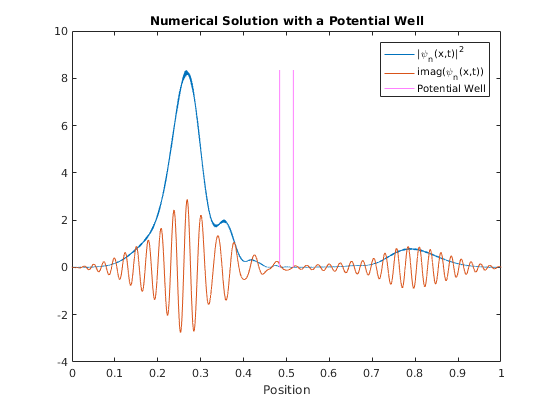
\includegraphics[width=1\textwidth]{../src/plots/squareBarrPlot.png}
		\caption{The numerical solution of $|\psi_n(x,t)|^2$ after it has hit the square barrier.}
		\label{fig:squareBarrfPlot}
	\end{subfigure}
	\begin{subfigure}{.9\linewidth}
		\setlength\figureheight{.5\linewidth}
		\setlength\figurewidth{.9\linewidth}
		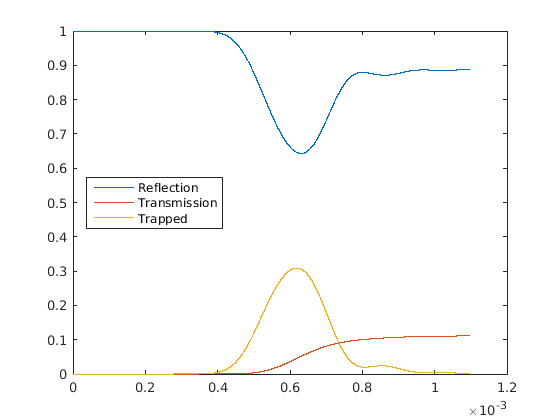
\includegraphics[width=1\textwidth]{../src/plots/squareBarrTR.png}
		\caption{Here we clearly see the transmission and reflection before and after the wave function hits the square barrier.}
		\label{fig:squareBarrTR}
	\end{subfigure}
	\label{fig:squareBarr}
	\caption{Here we depict the effect of the wave function hitting the square barrier. Note in figure \ref{fig:squareBarrTR} how a certain part of the wave function is trapped inside for while before a large part is reflected and a small part tunnels through.}
\end{figure}


\section{The effect of changing $k_0$}
In figure \ref{fig:k0} we can se how the constant $k_0$ affect the transmission and reflection of the wave function. It's clear that with a larger $k_0$ the transmission seem to approach nil while thee the reflection then of course are approaching total reflection.
\begin{figure}[H]
	\centering
	\setlength\figureheight{.5\linewidth}
	\setlength\figurewidth{.9\linewidth}
	\input{../src/plots/trvk0Plot.tikz}
	\caption{The reflektion and transmission through the potential well depending on the value of $k_0$}
	\label{fig:k0}
\end{figure}


\end{document}
